\PassOptionsToPackage{unicode=true}{hyperref} % options for packages loaded elsewhere
\PassOptionsToPackage{hyphens}{url}
%
\documentclass[]{book}
\usepackage{lmodern}
\usepackage{amssymb,amsmath}
\usepackage{ifxetex,ifluatex}
\usepackage{fixltx2e} % provides \textsubscript
\ifnum 0\ifxetex 1\fi\ifluatex 1\fi=0 % if pdftex
  \usepackage[T1]{fontenc}
  \usepackage[utf8]{inputenc}
  \usepackage{textcomp} % provides euro and other symbols
\else % if luatex or xelatex
  \usepackage{unicode-math}
  \defaultfontfeatures{Ligatures=TeX,Scale=MatchLowercase}
\fi
% use upquote if available, for straight quotes in verbatim environments
\IfFileExists{upquote.sty}{\usepackage{upquote}}{}
% use microtype if available
\IfFileExists{microtype.sty}{%
\usepackage[]{microtype}
\UseMicrotypeSet[protrusion]{basicmath} % disable protrusion for tt fonts
}{}
\IfFileExists{parskip.sty}{%
\usepackage{parskip}
}{% else
\setlength{\parindent}{0pt}
\setlength{\parskip}{6pt plus 2pt minus 1pt}
}
\usepackage{hyperref}
\hypersetup{
            pdftitle={Diagnostics Supplemental Material},
            pdfauthor={Jose Guadalupe Hernandez},
            pdfborder={0 0 0},
            breaklinks=true}
\urlstyle{same}  % don't use monospace font for urls
\usepackage{color}
\usepackage{fancyvrb}
\newcommand{\VerbBar}{|}
\newcommand{\VERB}{\Verb[commandchars=\\\{\}]}
\DefineVerbatimEnvironment{Highlighting}{Verbatim}{commandchars=\\\{\}}
% Add ',fontsize=\small' for more characters per line
\usepackage{framed}
\definecolor{shadecolor}{RGB}{248,248,248}
\newenvironment{Shaded}{\begin{snugshade}}{\end{snugshade}}
\newcommand{\AlertTok}[1]{\textcolor[rgb]{0.94,0.16,0.16}{#1}}
\newcommand{\AnnotationTok}[1]{\textcolor[rgb]{0.56,0.35,0.01}{\textbf{\textit{#1}}}}
\newcommand{\AttributeTok}[1]{\textcolor[rgb]{0.77,0.63,0.00}{#1}}
\newcommand{\BaseNTok}[1]{\textcolor[rgb]{0.00,0.00,0.81}{#1}}
\newcommand{\BuiltInTok}[1]{#1}
\newcommand{\CharTok}[1]{\textcolor[rgb]{0.31,0.60,0.02}{#1}}
\newcommand{\CommentTok}[1]{\textcolor[rgb]{0.56,0.35,0.01}{\textit{#1}}}
\newcommand{\CommentVarTok}[1]{\textcolor[rgb]{0.56,0.35,0.01}{\textbf{\textit{#1}}}}
\newcommand{\ConstantTok}[1]{\textcolor[rgb]{0.00,0.00,0.00}{#1}}
\newcommand{\ControlFlowTok}[1]{\textcolor[rgb]{0.13,0.29,0.53}{\textbf{#1}}}
\newcommand{\DataTypeTok}[1]{\textcolor[rgb]{0.13,0.29,0.53}{#1}}
\newcommand{\DecValTok}[1]{\textcolor[rgb]{0.00,0.00,0.81}{#1}}
\newcommand{\DocumentationTok}[1]{\textcolor[rgb]{0.56,0.35,0.01}{\textbf{\textit{#1}}}}
\newcommand{\ErrorTok}[1]{\textcolor[rgb]{0.64,0.00,0.00}{\textbf{#1}}}
\newcommand{\ExtensionTok}[1]{#1}
\newcommand{\FloatTok}[1]{\textcolor[rgb]{0.00,0.00,0.81}{#1}}
\newcommand{\FunctionTok}[1]{\textcolor[rgb]{0.00,0.00,0.00}{#1}}
\newcommand{\ImportTok}[1]{#1}
\newcommand{\InformationTok}[1]{\textcolor[rgb]{0.56,0.35,0.01}{\textbf{\textit{#1}}}}
\newcommand{\KeywordTok}[1]{\textcolor[rgb]{0.13,0.29,0.53}{\textbf{#1}}}
\newcommand{\NormalTok}[1]{#1}
\newcommand{\OperatorTok}[1]{\textcolor[rgb]{0.81,0.36,0.00}{\textbf{#1}}}
\newcommand{\OtherTok}[1]{\textcolor[rgb]{0.56,0.35,0.01}{#1}}
\newcommand{\PreprocessorTok}[1]{\textcolor[rgb]{0.56,0.35,0.01}{\textit{#1}}}
\newcommand{\RegionMarkerTok}[1]{#1}
\newcommand{\SpecialCharTok}[1]{\textcolor[rgb]{0.00,0.00,0.00}{#1}}
\newcommand{\SpecialStringTok}[1]{\textcolor[rgb]{0.31,0.60,0.02}{#1}}
\newcommand{\StringTok}[1]{\textcolor[rgb]{0.31,0.60,0.02}{#1}}
\newcommand{\VariableTok}[1]{\textcolor[rgb]{0.00,0.00,0.00}{#1}}
\newcommand{\VerbatimStringTok}[1]{\textcolor[rgb]{0.31,0.60,0.02}{#1}}
\newcommand{\WarningTok}[1]{\textcolor[rgb]{0.56,0.35,0.01}{\textbf{\textit{#1}}}}
\usepackage{longtable,booktabs}
% Fix footnotes in tables (requires footnote package)
\IfFileExists{footnote.sty}{\usepackage{footnote}\makesavenoteenv{longtable}}{}
\usepackage{graphicx,grffile}
\makeatletter
\def\maxwidth{\ifdim\Gin@nat@width>\linewidth\linewidth\else\Gin@nat@width\fi}
\def\maxheight{\ifdim\Gin@nat@height>\textheight\textheight\else\Gin@nat@height\fi}
\makeatother
% Scale images if necessary, so that they will not overflow the page
% margins by default, and it is still possible to overwrite the defaults
% using explicit options in \includegraphics[width, height, ...]{}
\setkeys{Gin}{width=\maxwidth,height=\maxheight,keepaspectratio}
\setlength{\emergencystretch}{3em}  % prevent overfull lines
\providecommand{\tightlist}{%
  \setlength{\itemsep}{0pt}\setlength{\parskip}{0pt}}
\setcounter{secnumdepth}{5}
% Redefines (sub)paragraphs to behave more like sections
\ifx\paragraph\undefined\else
\let\oldparagraph\paragraph
\renewcommand{\paragraph}[1]{\oldparagraph{#1}\mbox{}}
\fi
\ifx\subparagraph\undefined\else
\let\oldsubparagraph\subparagraph
\renewcommand{\subparagraph}[1]{\oldsubparagraph{#1}\mbox{}}
\fi

% set default figure placement to htbp
\makeatletter
\def\fps@figure{htbp}
\makeatother

\usepackage[]{natbib}
\bibliographystyle{apalike}

\title{Diagnostics Supplemental Material}
\author{Jose Guadalupe Hernandez}
\date{2023-01-31}

\begin{document}
\maketitle

{
\setcounter{tocdepth}{1}
\tableofcontents
}
\hypertarget{introduction}{%
\chapter{Introduction}\label{introduction}}

This is the supplemental material associated with our 2022 ECJ contribution entitled, \emph{A suite of diagnostic metrics for characterizing selection schemes}.
Preprint \href{https://arxiv.org/pdf/2204.13839.pdf}{here}.

\hypertarget{about-our-supplemental-material}{%
\section{About our supplemental material}\label{about-our-supplemental-material}}

This supplemental material is hosted on \href{https://github.com}{GitHub} using GitHub pages.
The source code and configuration files used to generate this supplemental material can be found in \href{https://github.com/jgh9094/ECJ-2022-suite-of-diagnostics-for-selection-schemes}{this GitHub repository}.
We compiled our data analyses and supplemental documentation into this nifty web-accessible book using \href{https://bookdown.org/}{bookdown}.

Our supplemental material includes the following paper figures and statistics:

\begin{itemize}
\tightlist
\item
  Exploitation rate results (Section \ref{exploitation-rate-results})
\item
  Ordered exploitation results (Section \ref{ordered-exploitation-results})
\item
  Contradictory objectives results (Section \ref{contradictory-objectives-results})
\item
  Multi-path exploration results (Section \ref{multi-path-exploration-results})
\item
  Multi-valley crossing results (Section \ref{multi-valley-crossing-results})
\end{itemize}

Additionally, our supplemental material includes the results from parameter tuning selection schemes:

\begin{itemize}
\tightlist
\item
  Truncation selection (Section \ref{truncation-selection})
\item
  Tournament selection sharing (Section \ref{tournament-selection})
\item
  Genotypic fitness sharing (Section \ref{genotypic-fitness-sharing})
\item
  Phenotypic fitness sharing (Section \ref{phenotypic-fitness-sharing})
\item
  Nondominated sorting (Section \ref{nondominated-sorting})
\item
  Novelty search (Section \ref{novelty-search})
\end{itemize}

\hypertarget{contributing-authors}{%
\section{Contributing authors}\label{contributing-authors}}

\begin{itemize}
\tightlist
\item
  \href{https://jgh9094.github.io/}{Jose Guadalupe Hernandez}
\item
  \href{https://lalejini.com}{Alexander Lalejini}
\item
  \href{http://ofria.com}{Charles Ofria}
\end{itemize}

\hypertarget{research-overview}{%
\section{Research overview}\label{research-overview}}

\textbf{Abstract}:

Evolutionary algorithms typically consist of multiple interacting components, where each component influences an algorithm's problem-solving abilities.
Understanding how each component of an evolutionary algorithm influences problem-solving success can improve our ability to target particular problem domains.
Benchmark suites provide insights into an evolutionary algorithm's problem-solving capabilities, but benchmarking problems often have complex search space topologies, making it difficult to isolate and test an algorithm's strengths and weaknesses.
Our work focuses on diagnosing selection schemes, which identify individuals to contribute genetic material to the next generation, thus driving an evolutionary algorithm's search strategy.
We introduce four diagnostics for empirically testing the strengths and weaknesses of selection schemes: the exploitation rate diagnostic, ordered exploitation rate diagnostic, contradictory objectives diagnostic, and the multi-path exploration diagnostic.
Each diagnostic is a handcrafted search space designed to isolate and measure the relative exploitation and exploration characteristics of selection schemes.
Here, we use our diagnostics to evaluate six population selection methods: truncation selection, tournament selection, fitness sharing, lexicase selection, nondominated sorting, and novelty search.
Expectedly, tournament and truncation selection excelled at gradient exploitation but poorly explored search spaces, while novelty search excelled at exploration but failed to exploit gradients.
Fitness sharing performed poorly across all diagnostics, suggesting poor overall exploitation and exploration abilities.
Nondominated sorting was best for maintaining diverse populations comprised of individuals inhabiting multiple optima, but struggled to effectively exploit gradients.
Lexicase selection balanced search space exploration without sacrificing exploitation, generally performing well across diagnostics.
Our work demonstrates the value of diagnostics for building a deeper understanding of selection schemes, which can then be used to improve or develop new selection methods.

\hypertarget{computer-setup}{%
\section{Computer Setup}\label{computer-setup}}

These analyses were conducted in the following computing environment:

\begin{Shaded}
\begin{Highlighting}[]
\KeywordTok{print}\NormalTok{(version)}
\end{Highlighting}
\end{Shaded}

\begin{verbatim}
##                _                                          
## platform       x86_64-pc-linux-gnu                        
## arch           x86_64                                     
## os             linux-gnu                                  
## system         x86_64, linux-gnu                          
## status         Patched                                    
## major          4                                          
## minor          2.2                                        
## year           2022                                       
## month          11                                         
## day            10                                         
## svn rev        83330                                      
## language       R                                          
## version.string R version 4.2.2 Patched (2022-11-10 r83330)
## nickname       Innocent and Trusting
\end{verbatim}

\hypertarget{experimental-setup}{%
\section{Experimental setup}\label{experimental-setup}}

Setting up required variables variables.

\begin{Shaded}
\begin{Highlighting}[]
\CommentTok{# includes}

\KeywordTok{library}\NormalTok{(plyr)}
\KeywordTok{library}\NormalTok{(dplyr)}
\end{Highlighting}
\end{Shaded}

\begin{verbatim}
## 
## Attaching package: 'dplyr'
\end{verbatim}

\begin{verbatim}
## The following objects are masked from 'package:plyr':
## 
##     arrange, count, desc, failwith, id, mutate, rename, summarise,
##     summarize
\end{verbatim}

\begin{verbatim}
## The following objects are masked from 'package:stats':
## 
##     filter, lag
\end{verbatim}

\begin{verbatim}
## The following objects are masked from 'package:base':
## 
##     intersect, setdiff, setequal, union
\end{verbatim}

\begin{Shaded}
\begin{Highlighting}[]
\KeywordTok{library}\NormalTok{(tidyverse)}
\end{Highlighting}
\end{Shaded}

\begin{verbatim}
## -- Attaching packages --------------------------------------- tidyverse 1.3.2
## --
\end{verbatim}

\begin{verbatim}
## v ggplot2 3.4.0     v purrr   1.0.1
## v tibble  3.1.8     v stringr 1.5.0
## v tidyr   1.3.0     v forcats 1.0.0
## v readr   2.1.3     
## -- Conflicts ------------------------------------------ tidyverse_conflicts() --
## x dplyr::arrange()   masks plyr::arrange()
## x purrr::compact()   masks plyr::compact()
## x dplyr::count()     masks plyr::count()
## x dplyr::desc()      masks plyr::desc()
## x dplyr::failwith()  masks plyr::failwith()
## x dplyr::filter()    masks stats::filter()
## x dplyr::id()        masks plyr::id()
## x dplyr::lag()       masks stats::lag()
## x dplyr::mutate()    masks plyr::mutate()
## x dplyr::rename()    masks plyr::rename()
## x dplyr::summarise() masks plyr::summarise()
## x dplyr::summarize() masks plyr::summarize()
\end{verbatim}

\begin{Shaded}
\begin{Highlighting}[]
\CommentTok{# graph variables}
\NormalTok{SHAPE =}\StringTok{ }\KeywordTok{c}\NormalTok{(}\DecValTok{5}\NormalTok{,}\DecValTok{3}\NormalTok{,}\DecValTok{1}\NormalTok{,}\DecValTok{2}\NormalTok{,}\DecValTok{6}\NormalTok{,}\DecValTok{0}\NormalTok{,}\DecValTok{4}\NormalTok{,}\DecValTok{20}\NormalTok{,}\DecValTok{1}\NormalTok{)}
\NormalTok{cb_palette <-}\StringTok{ }\KeywordTok{c}\NormalTok{(}\StringTok{'#332288'}\NormalTok{,}\StringTok{'#88CCEE'}\NormalTok{,}\StringTok{'#EE7733'}\NormalTok{,}\StringTok{'#EE3377'}\NormalTok{,}\StringTok{'#117733'}\NormalTok{,}\StringTok{'#882255'}\NormalTok{,}\StringTok{'#44AA99'}\NormalTok{,}\StringTok{'#CCBB44'}\NormalTok{, }\StringTok{'#000000'}\NormalTok{)}
\NormalTok{mvc_col =}\StringTok{ }\KeywordTok{c}\NormalTok{(}\StringTok{'#1A85FF'}\NormalTok{,}\StringTok{'#D41159'}\NormalTok{)}
\NormalTok{TSIZE =}\StringTok{ }\DecValTok{26}
\NormalTok{p_theme <-}\StringTok{ }\KeywordTok{theme}\NormalTok{(}
  \DataTypeTok{text =} \KeywordTok{element_text}\NormalTok{(}\DataTypeTok{size =} \DecValTok{28}\NormalTok{),}
  \DataTypeTok{plot.title =} \KeywordTok{element_text}\NormalTok{( }\DataTypeTok{face =} \StringTok{"bold"}\NormalTok{, }\DataTypeTok{size =} \DecValTok{22}\NormalTok{, }\DataTypeTok{hjust=}\FloatTok{0.5}\NormalTok{),}
  \DataTypeTok{panel.border =} \KeywordTok{element_blank}\NormalTok{(),}
  \DataTypeTok{panel.grid.minor =} \KeywordTok{element_blank}\NormalTok{(),}
  \DataTypeTok{legend.title=}\KeywordTok{element_text}\NormalTok{(}\DataTypeTok{size=}\DecValTok{22}\NormalTok{),}
  \DataTypeTok{legend.text=}\KeywordTok{element_text}\NormalTok{(}\DataTypeTok{size=}\DecValTok{23}\NormalTok{),}
  \DataTypeTok{axis.title =} \KeywordTok{element_text}\NormalTok{(}\DataTypeTok{size=}\DecValTok{23}\NormalTok{),}
  \DataTypeTok{axis.text =} \KeywordTok{element_text}\NormalTok{(}\DataTypeTok{size=}\DecValTok{22}\NormalTok{),}
  \DataTypeTok{legend.position=}\StringTok{"bottom"}\NormalTok{,}
  \DataTypeTok{panel.background =} \KeywordTok{element_rect}\NormalTok{(}\DataTypeTok{fill =} \StringTok{"#f1f2f5"}\NormalTok{,}
                                  \DataTypeTok{colour =} \StringTok{"white"}\NormalTok{,}
                                  \DataTypeTok{size =} \FloatTok{0.5}\NormalTok{, }\DataTypeTok{linetype =} \StringTok{"solid"}\NormalTok{)}
\NormalTok{)}
\end{Highlighting}
\end{Shaded}

\begin{verbatim}
## Warning: The `size` argument of `element_rect()` is deprecated as of ggplot2 3.4.0.
## i Please use the `linewidth` argument instead.
\end{verbatim}

\begin{Shaded}
\begin{Highlighting}[]
\CommentTok{# default variables}
\NormalTok{REPLICATES =}\StringTok{ }\DecValTok{50}
\NormalTok{DIMENSIONALITY =}\StringTok{ }\DecValTok{100}

\CommentTok{# selection scheme related stuff}
\NormalTok{ACRON =}\StringTok{ }\KeywordTok{tolower}\NormalTok{(}\KeywordTok{c}\NormalTok{(}\StringTok{'TRU'}\NormalTok{,}\StringTok{'TOR'}\NormalTok{,}\StringTok{'LEX'}\NormalTok{,}\StringTok{'GFS'}\NormalTok{,}\StringTok{'PFS'}\NormalTok{,}\StringTok{'NDS'}\NormalTok{,}\StringTok{'NOV'}\NormalTok{,}\StringTok{'RAN'}\NormalTok{))}
\NormalTok{NAMES =}\StringTok{ }\KeywordTok{c}\NormalTok{(}\StringTok{'Truncation (tru)'}\NormalTok{,}\StringTok{'Tournament (tor)'}\NormalTok{,}\StringTok{'Lexicase (lex)'}\NormalTok{, }\StringTok{'Genotypic Fitness Sharing (gfs)'}\NormalTok{,}\StringTok{'Phenotypic Fitness Sharing (pfs)'}\NormalTok{,}\StringTok{'Nondominated Sorting (nds)'}\NormalTok{,}\StringTok{'Novelty Search (nov)'}\NormalTok{,}\StringTok{'Random (ran)'}\NormalTok{)}
\NormalTok{SCHEME =}\StringTok{ }\KeywordTok{c}\NormalTok{(}\StringTok{'TRUNCATION'}\NormalTok{,}\StringTok{'TOURNAMENT'}\NormalTok{,}\StringTok{'LEXICASE'}\NormalTok{,}\StringTok{'FITSHARING_G'}\NormalTok{,}\StringTok{'FITSHARING_P'}\NormalTok{,}\StringTok{'NONDOMINATEDSORTING'}\NormalTok{,}\StringTok{'NOVELTY'}\NormalTok{,}\StringTok{'TOURNAMENT'}\NormalTok{)}
\NormalTok{ORDER =}\StringTok{ }\KeywordTok{c}\NormalTok{(}\StringTok{'Truncation (tru)'}\NormalTok{,}\StringTok{'Tournament (tor)'}\NormalTok{,}\StringTok{'Lexicase (lex)'}\NormalTok{, }\StringTok{'Genotypic Fitness Sharing (gfs)'}\NormalTok{,}\StringTok{'Phenotypic Fitness Sharing (pfs)'}\NormalTok{,}\StringTok{'Nondominated Sorting (nds)'}\NormalTok{,}\StringTok{'Novelty Search (nov)'}\NormalTok{,}\StringTok{'Random (ran)'}\NormalTok{)}

\CommentTok{# selection scheme parameters}
\NormalTok{TR_LIST =}\StringTok{ }\KeywordTok{c}\NormalTok{(}\DecValTok{1}\NormalTok{, }\DecValTok{2}\NormalTok{, }\DecValTok{4}\NormalTok{, }\DecValTok{8}\NormalTok{, }\DecValTok{16}\NormalTok{, }\DecValTok{32}\NormalTok{, }\DecValTok{64}\NormalTok{, }\DecValTok{128}\NormalTok{, }\DecValTok{256}\NormalTok{)}
\NormalTok{TS_LIST =}\StringTok{ }\KeywordTok{c}\NormalTok{(}\DecValTok{2}\NormalTok{, }\DecValTok{4}\NormalTok{, }\DecValTok{8}\NormalTok{, }\DecValTok{16}\NormalTok{, }\DecValTok{32}\NormalTok{, }\DecValTok{64}\NormalTok{, }\DecValTok{128}\NormalTok{, }\DecValTok{256}\NormalTok{)}
\NormalTok{FS_LIST =}\StringTok{ }\KeywordTok{c}\NormalTok{(}\FloatTok{0.0}\NormalTok{, }\FloatTok{0.1}\NormalTok{, }\FloatTok{0.3}\NormalTok{, }\FloatTok{0.6}\NormalTok{, }\FloatTok{1.2}\NormalTok{, }\FloatTok{2.5}\NormalTok{, }\FloatTok{5.0}\NormalTok{)}
\NormalTok{ND_LIST =}\StringTok{ }\KeywordTok{c}\NormalTok{(}\FloatTok{0.0}\NormalTok{, }\FloatTok{0.1}\NormalTok{, }\FloatTok{0.3}\NormalTok{, }\FloatTok{0.6}\NormalTok{, }\FloatTok{1.2}\NormalTok{, }\FloatTok{2.5}\NormalTok{, }\FloatTok{5.0}\NormalTok{)}
\NormalTok{NS_LIST =}\StringTok{ }\KeywordTok{c}\NormalTok{(}\DecValTok{1}\NormalTok{, }\DecValTok{2}\NormalTok{, }\DecValTok{4}\NormalTok{, }\DecValTok{8}\NormalTok{, }\DecValTok{15}\NormalTok{, }\DecValTok{30}\NormalTok{)}

\CommentTok{# selection scheme parameter we are looking for}
\NormalTok{PARAM =}\StringTok{ }\KeywordTok{c}\NormalTok{(}\StringTok{'8'}\NormalTok{, }\StringTok{'8'}\NormalTok{, }\StringTok{'0.0'}\NormalTok{, }\StringTok{'0.3'}\NormalTok{, }\StringTok{'0.3'}\NormalTok{, }\StringTok{'0.3'}\NormalTok{, }\StringTok{'15'}\NormalTok{, }\StringTok{'1'}\NormalTok{)}

\CommentTok{# for diagnostic loops}
\NormalTok{DIAGNOSTIC =}\StringTok{ }\KeywordTok{tolower}\NormalTok{(}\KeywordTok{c}\NormalTok{(}\StringTok{'EXPLOITATION_RATE'}\NormalTok{, }\StringTok{'ORDERED_EXPLOITATION'}\NormalTok{, }\StringTok{'CONTRADICTORY_OBJECTIVES'}\NormalTok{, }\StringTok{'MULTIPATH_EXPLORATION'}\NormalTok{))}

\CommentTok{# data diractory for gh-pages}
\NormalTok{DATA_DIR =}\StringTok{ '/opt/ECJ-2022-suite-of-diagnostics-for-selection-schemes/DATA-FINAL/'}

\CommentTok{######################################################################################}
\CommentTok{# go through each diagnostic and collect over time data for cross comparison (cc)}
\KeywordTok{print}\NormalTok{(}\StringTok{'Collecting over time data...'}\NormalTok{)}
\end{Highlighting}
\end{Shaded}

\begin{verbatim}
## [1] "Collecting over time data..."
\end{verbatim}

\begin{Shaded}
\begin{Highlighting}[]
\NormalTok{cc_over_time =}\StringTok{ }\KeywordTok{data.frame}\NormalTok{()}
\NormalTok{cc_over_time_mvc =}\StringTok{ }\KeywordTok{data.frame}\NormalTok{()}
\ControlFlowTok{for}\NormalTok{(diagnostic }\ControlFlowTok{in}\NormalTok{ DIAGNOSTIC)}
\NormalTok{\{}
  \KeywordTok{print}\NormalTok{(}\KeywordTok{paste}\NormalTok{(}\StringTok{'DIAGNOSTIC'}\NormalTok{,diagnostic))}
  \ControlFlowTok{for}\NormalTok{(i }\ControlFlowTok{in} \DecValTok{1}\OperatorTok{:}\DecValTok{8}\NormalTok{)}
\NormalTok{  \{}
    \KeywordTok{print}\NormalTok{(}\KeywordTok{paste}\NormalTok{(}\StringTok{'SCHEME:'}\NormalTok{,SCHEME[i]))}
\NormalTok{    dir =}\StringTok{ }\KeywordTok{paste}\NormalTok{(DATA_DIR,}\StringTok{'NO-MVC/'}\NormalTok{,SCHEME[i],}\StringTok{'/over-time-'}\NormalTok{,diagnostic,}\StringTok{'-'}\NormalTok{, }\KeywordTok{tolower}\NormalTok{(SCHEME[i]), }\StringTok{'.csv'}\NormalTok{, }\DataTypeTok{sep =} \StringTok{""}\NormalTok{, }\DataTypeTok{collapse =} \OtherTok{NULL}\NormalTok{)}
\NormalTok{    dir_mvc =}\StringTok{ }\KeywordTok{paste}\NormalTok{(DATA_DIR,}\StringTok{'MVC/'}\NormalTok{,SCHEME[i],}\StringTok{'/over-time-'}\NormalTok{,diagnostic,}\StringTok{'-'}\NormalTok{, }\KeywordTok{tolower}\NormalTok{(SCHEME[i]), }\StringTok{'.csv'}\NormalTok{, }\DataTypeTok{sep =} \StringTok{""}\NormalTok{, }\DataTypeTok{collapse =} \OtherTok{NULL}\NormalTok{)}

    \CommentTok{# read csv}
\NormalTok{    df =}\StringTok{ }\KeywordTok{read.csv}\NormalTok{(dir, }\DataTypeTok{header =} \OtherTok{TRUE}\NormalTok{, }\DataTypeTok{stringsAsFactors =} \OtherTok{FALSE}\NormalTok{)}
\NormalTok{    df_mvc =}\StringTok{ }\KeywordTok{read.csv}\NormalTok{(dir_mvc, }\DataTypeTok{header =} \OtherTok{TRUE}\NormalTok{, }\DataTypeTok{stringsAsFactors =} \OtherTok{FALSE}\NormalTok{)}

    \CommentTok{# add names/tags}
\NormalTok{    df}\OperatorTok{$}\NormalTok{acron =}\StringTok{ }\NormalTok{ACRON[i]}
\NormalTok{    df}\OperatorTok{$}\StringTok{`}\DataTypeTok{Selection}\CharTok{\textbackslash{}n}\DataTypeTok{Scheme}\StringTok{`}\NormalTok{ =}\StringTok{ }\NormalTok{NAMES[i]}
\NormalTok{    df}\OperatorTok{$}\NormalTok{diagnostic =}\StringTok{ }\NormalTok{diagnostic}

\NormalTok{    df_mvc}\OperatorTok{$}\NormalTok{acron =}\StringTok{ }\NormalTok{ACRON[i]}
\NormalTok{    df_mvc}\OperatorTok{$}\StringTok{`}\DataTypeTok{Selection}\CharTok{\textbackslash{}n}\DataTypeTok{Scheme}\StringTok{`}\NormalTok{ =}\StringTok{ }\NormalTok{NAMES[i]}
\NormalTok{    df_mvc}\OperatorTok{$}\NormalTok{diagnostic =}\StringTok{ }\NormalTok{diagnostic}

    \CommentTok{# add to cc_over_time data frame}
    \ControlFlowTok{if}\NormalTok{(i }\OperatorTok{==}\StringTok{ }\DecValTok{3}\NormalTok{)}
\NormalTok{    \{}
\NormalTok{      cc_over_time =}\StringTok{ }\KeywordTok{rbind}\NormalTok{(cc_over_time, df)}
\NormalTok{      cc_over_time_mvc =}\StringTok{ }\KeywordTok{rbind}\NormalTok{(cc_over_time_mvc, df_mvc)}
\NormalTok{    \}}
    \ControlFlowTok{else}
\NormalTok{    \{}
\NormalTok{      cc_over_time =}\StringTok{ }\KeywordTok{rbind}\NormalTok{(cc_over_time, }\KeywordTok{filter}\NormalTok{(df, trt }\OperatorTok{==}\StringTok{ }\NormalTok{PARAM[i]))}
\NormalTok{      cc_over_time_mvc =}\StringTok{ }\KeywordTok{rbind}\NormalTok{(cc_over_time_mvc, }\KeywordTok{filter}\NormalTok{(df_mvc, trt }\OperatorTok{==}\StringTok{ }\NormalTok{PARAM[i]))}
\NormalTok{    \}}
\NormalTok{  \}}
  \KeywordTok{rm}\NormalTok{(df);  }\KeywordTok{rm}\NormalTok{(df_mvc);  }\KeywordTok{rm}\NormalTok{(dir);   }\KeywordTok{rm}\NormalTok{(dir_mvc)}
\NormalTok{\}}
\end{Highlighting}
\end{Shaded}

\begin{verbatim}
## [1] "DIAGNOSTIC exploitation_rate"
## [1] "SCHEME: TRUNCATION"
## [1] "SCHEME: TOURNAMENT"
## [1] "SCHEME: LEXICASE"
## [1] "SCHEME: FITSHARING_G"
## [1] "SCHEME: FITSHARING_P"
## [1] "SCHEME: NONDOMINATEDSORTING"
## [1] "SCHEME: NOVELTY"
## [1] "SCHEME: TOURNAMENT"
## [1] "DIAGNOSTIC ordered_exploitation"
## [1] "SCHEME: TRUNCATION"
## [1] "SCHEME: TOURNAMENT"
## [1] "SCHEME: LEXICASE"
## [1] "SCHEME: FITSHARING_G"
## [1] "SCHEME: FITSHARING_P"
## [1] "SCHEME: NONDOMINATEDSORTING"
## [1] "SCHEME: NOVELTY"
## [1] "SCHEME: TOURNAMENT"
## [1] "DIAGNOSTIC contradictory_objectives"
## [1] "SCHEME: TRUNCATION"
## [1] "SCHEME: TOURNAMENT"
## [1] "SCHEME: LEXICASE"
## [1] "SCHEME: FITSHARING_G"
## [1] "SCHEME: FITSHARING_P"
## [1] "SCHEME: NONDOMINATEDSORTING"
## [1] "SCHEME: NOVELTY"
## [1] "SCHEME: TOURNAMENT"
## [1] "DIAGNOSTIC multipath_exploration"
## [1] "SCHEME: TRUNCATION"
## [1] "SCHEME: TOURNAMENT"
## [1] "SCHEME: LEXICASE"
## [1] "SCHEME: FITSHARING_G"
## [1] "SCHEME: FITSHARING_P"
## [1] "SCHEME: NONDOMINATEDSORTING"
## [1] "SCHEME: NOVELTY"
## [1] "SCHEME: TOURNAMENT"
\end{verbatim}

\begin{Shaded}
\begin{Highlighting}[]
\NormalTok{cc_over_time}\OperatorTok{$}\StringTok{`}\DataTypeTok{Selection}\CharTok{\textbackslash{}n}\DataTypeTok{Scheme}\StringTok{`}\NormalTok{ <-}\StringTok{ }\KeywordTok{factor}\NormalTok{(cc_over_time}\OperatorTok{$}\StringTok{`}\DataTypeTok{Selection}\CharTok{\textbackslash{}n}\DataTypeTok{Scheme}\StringTok{`}\NormalTok{, }\DataTypeTok{levels =}\NormalTok{ ORDER)}
\NormalTok{cc_over_time}\OperatorTok{$}\NormalTok{acron <-}\StringTok{ }\KeywordTok{factor}\NormalTok{(cc_over_time}\OperatorTok{$}\NormalTok{acron, }\DataTypeTok{levels =}\NormalTok{ ACRON)}
\NormalTok{cc_over_time}\OperatorTok{$}\NormalTok{uni_str_pos =}\StringTok{ }\NormalTok{cc_over_time}\OperatorTok{$}\NormalTok{uni_str_pos }\OperatorTok{+}\StringTok{ }\NormalTok{cc_over_time}\OperatorTok{$}\NormalTok{arc_acti_gene }\OperatorTok{-}\StringTok{ }\NormalTok{cc_over_time}\OperatorTok{$}\NormalTok{overlap}
\NormalTok{cc_over_time =}\StringTok{ }\KeywordTok{subset}\NormalTok{(cc_over_time, }\DataTypeTok{select =} \OperatorTok{-}\KeywordTok{c}\NormalTok{(trt,pop_fit_avg,archive_cnt,pmin,pareto_cnt,arc_acti_gene,overlap))}

\NormalTok{cc_over_time_mvc}\OperatorTok{$}\StringTok{`}\DataTypeTok{Selection}\CharTok{\textbackslash{}n}\DataTypeTok{Scheme}\StringTok{`}\NormalTok{ <-}\StringTok{ }\KeywordTok{factor}\NormalTok{(cc_over_time}\OperatorTok{$}\StringTok{`}\DataTypeTok{Selection}\CharTok{\textbackslash{}n}\DataTypeTok{Scheme}\StringTok{`}\NormalTok{, }\DataTypeTok{levels =}\NormalTok{ ORDER)}
\NormalTok{cc_over_time_mvc}\OperatorTok{$}\NormalTok{acron <-}\StringTok{ }\KeywordTok{factor}\NormalTok{(cc_over_time}\OperatorTok{$}\NormalTok{acron, }\DataTypeTok{levels =}\NormalTok{ ACRON)}
\NormalTok{cc_over_time_mvc}\OperatorTok{$}\NormalTok{uni_str_pos =}\StringTok{ }\NormalTok{cc_over_time_mvc}\OperatorTok{$}\NormalTok{uni_str_pos }\OperatorTok{+}\StringTok{ }\NormalTok{cc_over_time_mvc}\OperatorTok{$}\NormalTok{arc_acti_gene }\OperatorTok{-}\StringTok{ }\NormalTok{cc_over_time_mvc}\OperatorTok{$}\NormalTok{overlap}
\NormalTok{cc_over_time_mvc =}\StringTok{ }\KeywordTok{subset}\NormalTok{(cc_over_time_mvc, }\DataTypeTok{select =} \OperatorTok{-}\KeywordTok{c}\NormalTok{(trt,pop_fit_avg,archive_cnt,pmin,pareto_cnt,arc_acti_gene,overlap))}


\CommentTok{######################################################################################}
\CommentTok{# go through each diagnostic and collect best over time for cross comparison (cc)}
\NormalTok{cc_best =}\StringTok{ }\KeywordTok{data.frame}\NormalTok{()}
\NormalTok{cc_best_mvc =}\StringTok{ }\KeywordTok{data.frame}\NormalTok{()}
\ControlFlowTok{for}\NormalTok{(diagnostic }\ControlFlowTok{in}\NormalTok{ DIAGNOSTIC)}
\NormalTok{\{}
  \KeywordTok{print}\NormalTok{(}\KeywordTok{paste}\NormalTok{(}\StringTok{'DIAGNOSTIC'}\NormalTok{,diagnostic))}
  \ControlFlowTok{for}\NormalTok{(i }\ControlFlowTok{in} \DecValTok{1}\OperatorTok{:}\DecValTok{8}\NormalTok{)}
\NormalTok{  \{}
    \KeywordTok{print}\NormalTok{(}\KeywordTok{paste}\NormalTok{(}\StringTok{'SCHEME:'}\NormalTok{,SCHEME[i]))}
\NormalTok{    dir =}\StringTok{ }\KeywordTok{paste}\NormalTok{(DATA_DIR,}\StringTok{'NO-MVC/'}\NormalTok{,SCHEME[i],}\StringTok{'/best-'}\NormalTok{,diagnostic,}\StringTok{'-'}\NormalTok{, }\KeywordTok{tolower}\NormalTok{(SCHEME[i]), }\StringTok{'.csv'}\NormalTok{, }\DataTypeTok{sep =} \StringTok{""}\NormalTok{, }\DataTypeTok{collapse =} \OtherTok{NULL}\NormalTok{)}
\NormalTok{    dir_mvc =}\StringTok{ }\KeywordTok{paste}\NormalTok{(DATA_DIR,}\StringTok{'MVC/'}\NormalTok{,SCHEME[i],}\StringTok{'/best-'}\NormalTok{,diagnostic,}\StringTok{'-'}\NormalTok{, }\KeywordTok{tolower}\NormalTok{(SCHEME[i]), }\StringTok{'.csv'}\NormalTok{, }\DataTypeTok{sep =} \StringTok{""}\NormalTok{, }\DataTypeTok{collapse =} \OtherTok{NULL}\NormalTok{)}

    \CommentTok{# read csv}
\NormalTok{    df =}\StringTok{ }\KeywordTok{read.csv}\NormalTok{(dir, }\DataTypeTok{header =} \OtherTok{TRUE}\NormalTok{, }\DataTypeTok{stringsAsFactors =} \OtherTok{FALSE}\NormalTok{)}
\NormalTok{    df_mvc =}\StringTok{ }\KeywordTok{read.csv}\NormalTok{(dir_mvc, }\DataTypeTok{header =} \OtherTok{TRUE}\NormalTok{, }\DataTypeTok{stringsAsFactors =} \OtherTok{FALSE}\NormalTok{)}

    \CommentTok{# add names/tags}
\NormalTok{    df}\OperatorTok{$}\NormalTok{acron =}\StringTok{ }\NormalTok{ACRON[i]}
\NormalTok{    df}\OperatorTok{$}\StringTok{`}\DataTypeTok{Selection}\CharTok{\textbackslash{}n}\DataTypeTok{Scheme}\StringTok{`}\NormalTok{ =}\StringTok{ }\NormalTok{NAMES[i]}
\NormalTok{    df}\OperatorTok{$}\NormalTok{diagnostic =}\StringTok{ }\NormalTok{diagnostic}
\NormalTok{    df =}\StringTok{ }\KeywordTok{subset}\NormalTok{(df, }\DataTypeTok{select =} \OperatorTok{-}\KeywordTok{c}\NormalTok{(Diagnostic,SEL) )}

\NormalTok{    df_mvc}\OperatorTok{$}\NormalTok{acron =}\StringTok{ }\NormalTok{ACRON[i]}
\NormalTok{    df_mvc}\OperatorTok{$}\StringTok{`}\DataTypeTok{Selection}\CharTok{\textbackslash{}n}\DataTypeTok{Scheme}\StringTok{`}\NormalTok{ =}\StringTok{ }\NormalTok{NAMES[i]}
\NormalTok{    df_mvc}\OperatorTok{$}\NormalTok{diagnostic =}\StringTok{ }\NormalTok{diagnostic}
\NormalTok{    df_mvc =}\StringTok{ }\KeywordTok{subset}\NormalTok{(df_mvc, }\DataTypeTok{select =} \OperatorTok{-}\KeywordTok{c}\NormalTok{(Diagnostic,SEL) )}

    \CommentTok{# add to cc_over_time data frame}
    \ControlFlowTok{if}\NormalTok{(i }\OperatorTok{==}\StringTok{ }\DecValTok{3}\NormalTok{)}
\NormalTok{    \{}
\NormalTok{      cc_best =}\StringTok{ }\KeywordTok{rbind}\NormalTok{(cc_best, df)}
\NormalTok{      cc_best_mvc =}\StringTok{ }\KeywordTok{rbind}\NormalTok{(cc_best_mvc, df_mvc)}
\NormalTok{    \}}
    \ControlFlowTok{else}
\NormalTok{    \{}
\NormalTok{      cc_best =}\StringTok{ }\KeywordTok{rbind}\NormalTok{(cc_best, }\KeywordTok{filter}\NormalTok{(df, trt }\OperatorTok{==}\StringTok{ }\NormalTok{PARAM[i]))}
\NormalTok{      cc_best_mvc =}\StringTok{ }\KeywordTok{rbind}\NormalTok{(cc_best_mvc, }\KeywordTok{filter}\NormalTok{(df_mvc, trt }\OperatorTok{==}\StringTok{ }\NormalTok{PARAM[i]))}
\NormalTok{    \}}
\NormalTok{  \}}
  \KeywordTok{rm}\NormalTok{(df);  }\KeywordTok{rm}\NormalTok{(df_mvc);  }\KeywordTok{rm}\NormalTok{(dir);   }\KeywordTok{rm}\NormalTok{(dir_mvc)}
\NormalTok{\}}
\end{Highlighting}
\end{Shaded}

\begin{verbatim}
## [1] "DIAGNOSTIC exploitation_rate"
## [1] "SCHEME: TRUNCATION"
## [1] "SCHEME: TOURNAMENT"
## [1] "SCHEME: LEXICASE"
## [1] "SCHEME: FITSHARING_G"
## [1] "SCHEME: FITSHARING_P"
## [1] "SCHEME: NONDOMINATEDSORTING"
## [1] "SCHEME: NOVELTY"
## [1] "SCHEME: TOURNAMENT"
## [1] "DIAGNOSTIC ordered_exploitation"
## [1] "SCHEME: TRUNCATION"
## [1] "SCHEME: TOURNAMENT"
## [1] "SCHEME: LEXICASE"
## [1] "SCHEME: FITSHARING_G"
## [1] "SCHEME: FITSHARING_P"
## [1] "SCHEME: NONDOMINATEDSORTING"
## [1] "SCHEME: NOVELTY"
## [1] "SCHEME: TOURNAMENT"
## [1] "DIAGNOSTIC contradictory_objectives"
## [1] "SCHEME: TRUNCATION"
## [1] "SCHEME: TOURNAMENT"
## [1] "SCHEME: LEXICASE"
## [1] "SCHEME: FITSHARING_G"
## [1] "SCHEME: FITSHARING_P"
## [1] "SCHEME: NONDOMINATEDSORTING"
## [1] "SCHEME: NOVELTY"
## [1] "SCHEME: TOURNAMENT"
## [1] "DIAGNOSTIC multipath_exploration"
## [1] "SCHEME: TRUNCATION"
## [1] "SCHEME: TOURNAMENT"
## [1] "SCHEME: LEXICASE"
## [1] "SCHEME: FITSHARING_G"
## [1] "SCHEME: FITSHARING_P"
## [1] "SCHEME: NONDOMINATEDSORTING"
## [1] "SCHEME: NOVELTY"
## [1] "SCHEME: TOURNAMENT"
\end{verbatim}

\begin{Shaded}
\begin{Highlighting}[]
\NormalTok{cc_best}\OperatorTok{$}\NormalTok{acron <-}\StringTok{ }\KeywordTok{factor}\NormalTok{(cc_best}\OperatorTok{$}\NormalTok{acron, }\DataTypeTok{levels =}\NormalTok{ ACRON)}
\NormalTok{cc_best =}\StringTok{ }\KeywordTok{subset}\NormalTok{(cc_best, }\DataTypeTok{select =} \OperatorTok{-}\KeywordTok{c}\NormalTok{(trt,gen))}
\NormalTok{cc_best =}\StringTok{ }\KeywordTok{filter}\NormalTok{(cc_best, col }\OperatorTok{==}\StringTok{ 'pop_fit_max'} \OperatorTok{|}\StringTok{ }\NormalTok{col }\OperatorTok{==}\StringTok{ 'pop_uni_obj'}\NormalTok{)}

\NormalTok{cc_best_mvc}\OperatorTok{$}\NormalTok{acron <-}\StringTok{ }\KeywordTok{factor}\NormalTok{(cc_best_mvc}\OperatorTok{$}\NormalTok{acron, }\DataTypeTok{levels =}\NormalTok{ ACRON)}
\NormalTok{cc_best_mvc =}\StringTok{ }\KeywordTok{subset}\NormalTok{(cc_best_mvc, }\DataTypeTok{select =} \OperatorTok{-}\KeywordTok{c}\NormalTok{(trt,gen))}
\NormalTok{cc_best_mvc =}\StringTok{ }\KeywordTok{subset}\NormalTok{(cc_best_mvc, col }\OperatorTok{==}\StringTok{ 'pop_fit_max'} \OperatorTok{|}\StringTok{ }\NormalTok{col }\OperatorTok{==}\StringTok{ 'pop_uni_obj'}\NormalTok{)}


\CommentTok{######################################################################################}
\CommentTok{# get generation a satisfactory solution is found for cross comparison (cc)}
\NormalTok{cc_ssf  =}\StringTok{ }\KeywordTok{data.frame}\NormalTok{()}
\ControlFlowTok{for}\NormalTok{(diagnostic }\ControlFlowTok{in}\NormalTok{ DIAGNOSTIC)}
\NormalTok{\{}
  \ControlFlowTok{if}\NormalTok{(diagnostic }\OperatorTok{==}\StringTok{ 'contradictory_objectives'} \OperatorTok{|}\StringTok{ }\NormalTok{diagnostic }\OperatorTok{==}\StringTok{ 'multipath_exploration'}\NormalTok{)}
\NormalTok{  \{}\ControlFlowTok{next}\NormalTok{\}}

  \KeywordTok{print}\NormalTok{(}\KeywordTok{paste}\NormalTok{(}\StringTok{'DIAGNOSTIC'}\NormalTok{,diagnostic))}
  \ControlFlowTok{for}\NormalTok{(i }\ControlFlowTok{in} \DecValTok{1}\OperatorTok{:}\DecValTok{8}\NormalTok{)}
\NormalTok{  \{}
    \KeywordTok{print}\NormalTok{(}\KeywordTok{paste}\NormalTok{(}\StringTok{'SCHEME:'}\NormalTok{,SCHEME[i]))}
\NormalTok{    dir =}\StringTok{ }\KeywordTok{paste}\NormalTok{(DATA_DIR,}\StringTok{'NO-MVC/'}\NormalTok{,SCHEME[i],}\StringTok{'/ssf-'}\NormalTok{,diagnostic,}\StringTok{'-'}\NormalTok{, }\KeywordTok{tolower}\NormalTok{(SCHEME[i]), }\StringTok{'.csv'}\NormalTok{, }\DataTypeTok{sep =} \StringTok{""}\NormalTok{, }\DataTypeTok{collapse =} \OtherTok{NULL}\NormalTok{)}

    \CommentTok{# read csv}
\NormalTok{    df =}\StringTok{ }\KeywordTok{read.csv}\NormalTok{(dir, }\DataTypeTok{header =} \OtherTok{TRUE}\NormalTok{, }\DataTypeTok{stringsAsFactors =} \OtherTok{FALSE}\NormalTok{)}

    \CommentTok{# add names/tags}
\NormalTok{    df}\OperatorTok{$}\NormalTok{acron =}\StringTok{ }\NormalTok{ACRON[i]}
\NormalTok{    df}\OperatorTok{$}\StringTok{`}\DataTypeTok{Selection}\CharTok{\textbackslash{}n}\DataTypeTok{Scheme}\StringTok{`}\NormalTok{ =}\StringTok{ }\NormalTok{NAMES[i]}
\NormalTok{    df}\OperatorTok{$}\NormalTok{diagnostic =}\StringTok{ }\NormalTok{diagnostic}
\NormalTok{    df =}\StringTok{ }\KeywordTok{subset}\NormalTok{(df, }\DataTypeTok{select =} \OperatorTok{-}\KeywordTok{c}\NormalTok{(Diagnostic,SEL) )}

    \CommentTok{# add to cc_over_time data frame}
    \ControlFlowTok{if}\NormalTok{(i }\OperatorTok{==}\StringTok{ }\DecValTok{3}\NormalTok{)}
\NormalTok{    \{}
\NormalTok{      cc_ssf =}\StringTok{ }\KeywordTok{rbind}\NormalTok{(cc_ssf, df)}
\NormalTok{    \}}
    \ControlFlowTok{else}
\NormalTok{    \{}
\NormalTok{      cc_ssf =}\StringTok{ }\KeywordTok{rbind}\NormalTok{(cc_ssf, }\KeywordTok{filter}\NormalTok{(df, trt }\OperatorTok{==}\StringTok{ }\NormalTok{PARAM[i]))}
\NormalTok{    \}}
\NormalTok{  \}}
  \KeywordTok{rm}\NormalTok{(df); }\KeywordTok{rm}\NormalTok{(dir);}
\NormalTok{\}}
\end{Highlighting}
\end{Shaded}

\begin{verbatim}
## [1] "DIAGNOSTIC exploitation_rate"
## [1] "SCHEME: TRUNCATION"
## [1] "SCHEME: TOURNAMENT"
## [1] "SCHEME: LEXICASE"
## [1] "SCHEME: FITSHARING_G"
## [1] "SCHEME: FITSHARING_P"
## [1] "SCHEME: NONDOMINATEDSORTING"
## [1] "SCHEME: NOVELTY"
## [1] "SCHEME: TOURNAMENT"
## [1] "DIAGNOSTIC ordered_exploitation"
## [1] "SCHEME: TRUNCATION"
## [1] "SCHEME: TOURNAMENT"
## [1] "SCHEME: LEXICASE"
## [1] "SCHEME: FITSHARING_G"
## [1] "SCHEME: FITSHARING_P"
## [1] "SCHEME: NONDOMINATEDSORTING"
## [1] "SCHEME: NOVELTY"
## [1] "SCHEME: TOURNAMENT"
\end{verbatim}

\begin{Shaded}
\begin{Highlighting}[]
\NormalTok{cc_ssf}\OperatorTok{$}\NormalTok{acron <-}\StringTok{ }\KeywordTok{factor}\NormalTok{(cc_ssf}\OperatorTok{$}\NormalTok{acron, }\DataTypeTok{levels =}\NormalTok{ ACRON)}
\NormalTok{cc_ssf =}\StringTok{ }\KeywordTok{subset}\NormalTok{(cc_ssf, }\DataTypeTok{select =} \OperatorTok{-}\KeywordTok{c}\NormalTok{(trt))}


\CommentTok{######################################################################################}
\CommentTok{# go through each scheme and collect over time data}
\NormalTok{ss_over_time =}\StringTok{ }\KeywordTok{data.frame}\NormalTok{()}
\NormalTok{ss_over_time_mvc =}\StringTok{ }\KeywordTok{data.frame}\NormalTok{()}
\ControlFlowTok{for}\NormalTok{(i }\ControlFlowTok{in} \DecValTok{1}\OperatorTok{:}\DecValTok{8}\NormalTok{)}
\NormalTok{\{}
  \CommentTok{# add to cc_over_time data frame}
  \ControlFlowTok{if}\NormalTok{(i }\OperatorTok{==}\StringTok{ }\DecValTok{3} \OperatorTok{|}\StringTok{ }\NormalTok{i }\OperatorTok{==}\StringTok{ }\DecValTok{8}\NormalTok{)}
\NormalTok{  \{}
    \ControlFlowTok{next}
\NormalTok{  \}}
  \KeywordTok{print}\NormalTok{(SCHEME[i])}
  \ControlFlowTok{for}\NormalTok{(diagnostic }\ControlFlowTok{in}\NormalTok{ DIAGNOSTIC)}
\NormalTok{  \{}
\NormalTok{    dir =}\StringTok{ }\KeywordTok{paste}\NormalTok{(DATA_DIR,}\StringTok{'NO-MVC/'}\NormalTok{,SCHEME[i],}\StringTok{'/over-time-'}\NormalTok{,diagnostic,}\StringTok{'-'}\NormalTok{, }\KeywordTok{tolower}\NormalTok{(SCHEME[i]), }\StringTok{'.csv'}\NormalTok{, }\DataTypeTok{sep =} \StringTok{""}\NormalTok{, }\DataTypeTok{collapse =} \OtherTok{NULL}\NormalTok{)}
\NormalTok{    dir_mvc =}\StringTok{ }\KeywordTok{paste}\NormalTok{(DATA_DIR,}\StringTok{'MVC/'}\NormalTok{,SCHEME[i],}\StringTok{'/over-time-'}\NormalTok{,diagnostic,}\StringTok{'-'}\NormalTok{, }\KeywordTok{tolower}\NormalTok{(SCHEME[i]), }\StringTok{'.csv'}\NormalTok{, }\DataTypeTok{sep =} \StringTok{""}\NormalTok{, }\DataTypeTok{collapse =} \OtherTok{NULL}\NormalTok{)}

    \CommentTok{# read csv}
\NormalTok{    df =}\StringTok{ }\KeywordTok{read.csv}\NormalTok{(dir, }\DataTypeTok{header =} \OtherTok{TRUE}\NormalTok{, }\DataTypeTok{stringsAsFactors =} \OtherTok{FALSE}\NormalTok{)}
\NormalTok{    df_mvc =}\StringTok{ }\KeywordTok{read.csv}\NormalTok{(dir_mvc, }\DataTypeTok{header =} \OtherTok{TRUE}\NormalTok{, }\DataTypeTok{stringsAsFactors =} \OtherTok{FALSE}\NormalTok{)}

    \CommentTok{# add names/tags}
\NormalTok{    df}\OperatorTok{$}\NormalTok{acron =}\StringTok{ }\NormalTok{ACRON[i]}
\NormalTok{    df}\OperatorTok{$}\NormalTok{diagnostic =}\StringTok{ }\NormalTok{diagnostic}

\NormalTok{    df_mvc}\OperatorTok{$}\NormalTok{acron =}\StringTok{ }\NormalTok{ACRON[i]}
\NormalTok{    df_mvc}\OperatorTok{$}\NormalTok{diagnostic =}\StringTok{ }\NormalTok{diagnostic}

\NormalTok{    ss_over_time =}\StringTok{ }\KeywordTok{rbind}\NormalTok{(ss_over_time, df)}
\NormalTok{    ss_over_time_mvc =}\StringTok{ }\KeywordTok{rbind}\NormalTok{(ss_over_time_mvc,df_mvc)}
\NormalTok{  \}}
  \KeywordTok{rm}\NormalTok{(df);  }\KeywordTok{rm}\NormalTok{(df_mvc);  }\KeywordTok{rm}\NormalTok{(dir);   }\KeywordTok{rm}\NormalTok{(dir_mvc)}
\NormalTok{\}}
\end{Highlighting}
\end{Shaded}

\begin{verbatim}
## [1] "TRUNCATION"
## [1] "TOURNAMENT"
## [1] "FITSHARING_G"
## [1] "FITSHARING_P"
## [1] "NONDOMINATEDSORTING"
## [1] "NOVELTY"
\end{verbatim}

\begin{Shaded}
\begin{Highlighting}[]
\CommentTok{# remove unused data}

\NormalTok{ss_over_time}\OperatorTok{$}\NormalTok{uni_str_pos =}\StringTok{ }\NormalTok{ss_over_time}\OperatorTok{$}\NormalTok{uni_str_pos }\OperatorTok{+}\StringTok{ }\NormalTok{ss_over_time}\OperatorTok{$}\NormalTok{arc_acti_gene }\OperatorTok{-}\StringTok{ }\NormalTok{ss_over_time}\OperatorTok{$}\NormalTok{overlap}
\NormalTok{ss_over_time =}\StringTok{ }\KeywordTok{subset}\NormalTok{(ss_over_time, }\DataTypeTok{select =} \OperatorTok{-}\KeywordTok{c}\NormalTok{(pop_fit_avg,archive_cnt,pmin,pareto_cnt,arc_acti_gene,overlap))}

\NormalTok{ss_over_time_mvc}\OperatorTok{$}\NormalTok{uni_str_pos =}\StringTok{ }\NormalTok{ss_over_time_mvc}\OperatorTok{$}\NormalTok{uni_str_pos }\OperatorTok{+}\StringTok{ }\NormalTok{ss_over_time_mvc}\OperatorTok{$}\NormalTok{arc_acti_gene }\OperatorTok{-}\StringTok{ }\NormalTok{ss_over_time_mvc}\OperatorTok{$}\NormalTok{overlap}
\NormalTok{ss_over_time_mvc =}\StringTok{ }\KeywordTok{subset}\NormalTok{(ss_over_time_mvc, }\DataTypeTok{select =} \OperatorTok{-}\KeywordTok{c}\NormalTok{(pop_fit_avg,archive_cnt,pmin,pareto_cnt,arc_acti_gene,overlap))}

\CommentTok{## tournament data frames}
\NormalTok{tor_ot <-}\StringTok{ }\KeywordTok{data.frame}\NormalTok{()}
\NormalTok{tor_ot <-}\StringTok{ }\KeywordTok{filter}\NormalTok{(ss_over_time, acron }\OperatorTok{==}\StringTok{ 'tor'} \OperatorTok{&}\StringTok{ }\NormalTok{trt }\OperatorTok{!=}\StringTok{ }\DecValTok{1}\NormalTok{)}
\NormalTok{tor_ot}\OperatorTok{$}\NormalTok{T <-}\StringTok{ }\KeywordTok{factor}\NormalTok{(tor_ot}\OperatorTok{$}\NormalTok{trt, }\DataTypeTok{levels =}\NormalTok{ TS_LIST)}
\NormalTok{tor_ot <-}\StringTok{ }\KeywordTok{subset}\NormalTok{(tor_ot, }\DataTypeTok{select =} \OperatorTok{-}\KeywordTok{c}\NormalTok{(acron,trt))}

\CommentTok{## truncation data frames}
\NormalTok{tru_ot <-}\StringTok{ }\KeywordTok{data.frame}\NormalTok{()}
\NormalTok{tru_ot <-}\StringTok{ }\KeywordTok{filter}\NormalTok{(ss_over_time, acron }\OperatorTok{==}\StringTok{ 'tru'}\NormalTok{)}
\NormalTok{tru_ot}\OperatorTok{$}\NormalTok{T <-}\StringTok{ }\KeywordTok{factor}\NormalTok{(tru_ot}\OperatorTok{$}\NormalTok{trt, }\DataTypeTok{levels =}\NormalTok{ TR_LIST)}
\NormalTok{tru_ot <-}\StringTok{ }\KeywordTok{subset}\NormalTok{(tru_ot, }\DataTypeTok{select =} \OperatorTok{-}\KeywordTok{c}\NormalTok{(acron,trt))}

\CommentTok{## genotypic fitness sharing data frames}
\NormalTok{gfs_ot <-}\StringTok{ }\KeywordTok{data.frame}\NormalTok{()}
\NormalTok{gfs_ot <-}\StringTok{ }\KeywordTok{filter}\NormalTok{(ss_over_time, acron }\OperatorTok{==}\StringTok{ 'gfs'}\NormalTok{)}
\NormalTok{gfs_ot}\OperatorTok{$}\NormalTok{Sigma <-}\StringTok{ }\KeywordTok{factor}\NormalTok{(gfs_ot}\OperatorTok{$}\NormalTok{trt, }\DataTypeTok{levels =}\NormalTok{ FS_LIST)}
\NormalTok{gfs_ot <-}\StringTok{ }\KeywordTok{subset}\NormalTok{(gfs_ot, }\DataTypeTok{select =} \OperatorTok{-}\KeywordTok{c}\NormalTok{(acron,trt))}

\CommentTok{## phenotypic fitness sharing data frames}
\NormalTok{pfs_ot <-}\StringTok{ }\KeywordTok{data.frame}\NormalTok{()}
\NormalTok{pfs_ot <-}\StringTok{ }\KeywordTok{filter}\NormalTok{(ss_over_time, acron }\OperatorTok{==}\StringTok{ 'pfs'}\NormalTok{)}
\NormalTok{pfs_ot}\OperatorTok{$}\NormalTok{Sigma <-}\StringTok{ }\KeywordTok{factor}\NormalTok{(pfs_ot}\OperatorTok{$}\NormalTok{trt, }\DataTypeTok{levels =}\NormalTok{ FS_LIST)}
\NormalTok{pfs_ot <-}\StringTok{ }\KeywordTok{subset}\NormalTok{(pfs_ot, }\DataTypeTok{select =} \OperatorTok{-}\KeywordTok{c}\NormalTok{(acron,trt))}


\CommentTok{## nodominated sorting data frames}
\NormalTok{nds_ot <-}\StringTok{ }\KeywordTok{data.frame}\NormalTok{()}
\NormalTok{nds_ot <-}\StringTok{ }\KeywordTok{filter}\NormalTok{(ss_over_time, acron }\OperatorTok{==}\StringTok{ 'nds'}\NormalTok{)}
\NormalTok{nds_ot}\OperatorTok{$}\NormalTok{Sigma <-}\StringTok{ }\KeywordTok{factor}\NormalTok{(nds_ot}\OperatorTok{$}\NormalTok{trt, }\DataTypeTok{levels =}\NormalTok{ ND_LIST)}
\NormalTok{nds_ot <-}\StringTok{ }\KeywordTok{subset}\NormalTok{(nds_ot, }\DataTypeTok{select =} \OperatorTok{-}\KeywordTok{c}\NormalTok{(acron,trt))}

\CommentTok{## novelty search data frames}
\NormalTok{nov_ot <-}\StringTok{ }\KeywordTok{data.frame}\NormalTok{()}
\NormalTok{nov_ot <-}\StringTok{ }\KeywordTok{filter}\NormalTok{(ss_over_time, acron }\OperatorTok{==}\StringTok{ 'nov'} \OperatorTok{&}\StringTok{ }\NormalTok{trt }\OperatorTok{!=}\StringTok{ }\DecValTok{0}\NormalTok{)}
\NormalTok{nov_ot}\OperatorTok{$}\NormalTok{K <-}\StringTok{ }\KeywordTok{factor}\NormalTok{(nov_ot}\OperatorTok{$}\NormalTok{trt, }\DataTypeTok{levels =}\NormalTok{ NS_LIST)}
\NormalTok{nov_ot <-}\StringTok{ }\KeywordTok{subset}\NormalTok{(nov_ot, }\DataTypeTok{select =} \OperatorTok{-}\KeywordTok{c}\NormalTok{(acron,trt))}

\CommentTok{## tournament data frames mvc}
\NormalTok{tor_ot_mvc <-}\StringTok{ }\KeywordTok{data.frame}\NormalTok{()}
\NormalTok{tor_ot_mvc <-}\StringTok{ }\KeywordTok{filter}\NormalTok{(ss_over_time_mvc, acron }\OperatorTok{==}\StringTok{ 'tor'} \OperatorTok{&}\StringTok{ }\NormalTok{trt }\OperatorTok{!=}\StringTok{ }\DecValTok{1}\NormalTok{)}
\NormalTok{tor_ot_mvc}\OperatorTok{$}\NormalTok{T <-}\StringTok{ }\KeywordTok{factor}\NormalTok{(tor_ot_mvc}\OperatorTok{$}\NormalTok{trt, }\DataTypeTok{levels =}\NormalTok{ TS_LIST)}
\NormalTok{tor_ot_mvc <-}\StringTok{ }\KeywordTok{subset}\NormalTok{(tor_ot_mvc, }\DataTypeTok{select =} \OperatorTok{-}\KeywordTok{c}\NormalTok{(acron,trt))}

\CommentTok{## truncation data frames mvc}
\NormalTok{tru_ot_mvc <-}\StringTok{ }\KeywordTok{data.frame}\NormalTok{()}
\NormalTok{tru_ot_mvc <-}\StringTok{ }\KeywordTok{filter}\NormalTok{(ss_over_time_mvc, acron }\OperatorTok{==}\StringTok{ 'tru'}\NormalTok{)}
\NormalTok{tru_ot_mvc}\OperatorTok{$}\NormalTok{T <-}\StringTok{ }\KeywordTok{factor}\NormalTok{(tru_ot_mvc}\OperatorTok{$}\NormalTok{trt, }\DataTypeTok{levels =}\NormalTok{ TR_LIST)}
\NormalTok{tru_ot_mvc <-}\StringTok{ }\KeywordTok{subset}\NormalTok{(tru_ot_mvc, }\DataTypeTok{select =} \OperatorTok{-}\KeywordTok{c}\NormalTok{(acron,trt))}

\CommentTok{## genotypic fitness sharing data frames mvc}
\NormalTok{gfs_ot_mvc <-}\StringTok{ }\KeywordTok{data.frame}\NormalTok{()}
\NormalTok{gfs_ot_mvc <-}\StringTok{ }\KeywordTok{filter}\NormalTok{(ss_over_time_mvc, acron }\OperatorTok{==}\StringTok{ 'gfs'}\NormalTok{)}
\NormalTok{gfs_ot_mvc}\OperatorTok{$}\NormalTok{Sigma <-}\StringTok{ }\KeywordTok{factor}\NormalTok{(gfs_ot_mvc}\OperatorTok{$}\NormalTok{trt, }\DataTypeTok{levels =}\NormalTok{ FS_LIST)}
\NormalTok{gfs_ot_mvc <-}\StringTok{ }\KeywordTok{subset}\NormalTok{(gfs_ot_mvc, }\DataTypeTok{select =} \OperatorTok{-}\KeywordTok{c}\NormalTok{(acron,trt))}

\CommentTok{## phenotypic fitness sharing data frames mvc}
\NormalTok{pfs_ot_mvc <-}\StringTok{ }\KeywordTok{data.frame}\NormalTok{()}
\NormalTok{pfs_ot_mvc <-}\StringTok{ }\KeywordTok{filter}\NormalTok{(ss_over_time_mvc, acron }\OperatorTok{==}\StringTok{ 'pfs'}\NormalTok{)}
\NormalTok{pfs_ot_mvc}\OperatorTok{$}\NormalTok{Sigma <-}\StringTok{ }\KeywordTok{factor}\NormalTok{(pfs_ot_mvc}\OperatorTok{$}\NormalTok{trt, }\DataTypeTok{levels =}\NormalTok{ FS_LIST)}
\NormalTok{pfs_ot_mvc <-}\StringTok{ }\KeywordTok{subset}\NormalTok{(pfs_ot_mvc, }\DataTypeTok{select =} \OperatorTok{-}\KeywordTok{c}\NormalTok{(acron,trt))}


\CommentTok{## nodominated sorting data frames mvc}
\NormalTok{nds_ot_mvc <-}\StringTok{ }\KeywordTok{data.frame}\NormalTok{()}
\NormalTok{nds_ot_mvc <-}\StringTok{ }\KeywordTok{filter}\NormalTok{(ss_over_time_mvc, acron }\OperatorTok{==}\StringTok{ 'nds'}\NormalTok{)}
\NormalTok{nds_ot_mvc}\OperatorTok{$}\NormalTok{Sigma <-}\StringTok{ }\KeywordTok{factor}\NormalTok{(nds_ot_mvc}\OperatorTok{$}\NormalTok{trt, }\DataTypeTok{levels =}\NormalTok{ ND_LIST)}
\NormalTok{nds_ot_mvc <-}\StringTok{ }\KeywordTok{subset}\NormalTok{(nds_ot_mvc, }\DataTypeTok{select =} \OperatorTok{-}\KeywordTok{c}\NormalTok{(acron,trt))}

\CommentTok{## novelty search data frames mvc}
\NormalTok{nov_ot_mvc <-}\StringTok{ }\KeywordTok{data.frame}\NormalTok{()}
\NormalTok{nov_ot_mvc <-}\StringTok{ }\KeywordTok{filter}\NormalTok{(ss_over_time_mvc, acron }\OperatorTok{==}\StringTok{ 'nov'} \OperatorTok{&}\StringTok{ }\NormalTok{trt }\OperatorTok{!=}\StringTok{ }\DecValTok{0}\NormalTok{)}
\NormalTok{nov_ot_mvc}\OperatorTok{$}\NormalTok{K <-}\StringTok{ }\KeywordTok{factor}\NormalTok{(nov_ot_mvc}\OperatorTok{$}\NormalTok{trt, }\DataTypeTok{levels =}\NormalTok{ NS_LIST)}
\NormalTok{nov_ot_mvc <-}\StringTok{ }\KeywordTok{subset}\NormalTok{(nov_ot_mvc, }\DataTypeTok{select =} \OperatorTok{-}\KeywordTok{c}\NormalTok{(acron,trt))}

\CommentTok{# clean up}
\KeywordTok{rm}\NormalTok{(ss_over_time_mvc)}
\KeywordTok{rm}\NormalTok{(ss_over_time)}


\CommentTok{######################################################################################}
\CommentTok{# go through each scheme and collect best data}
\NormalTok{ss_best =}\StringTok{ }\KeywordTok{data.frame}\NormalTok{()}
\NormalTok{ss_best_mvc =}\StringTok{ }\KeywordTok{data.frame}\NormalTok{()}
\ControlFlowTok{for}\NormalTok{(i }\ControlFlowTok{in} \DecValTok{1}\OperatorTok{:}\DecValTok{8}\NormalTok{)}
\NormalTok{\{}
  \CommentTok{# add to cc_best data frame}
  \ControlFlowTok{if}\NormalTok{(i }\OperatorTok{==}\StringTok{ }\DecValTok{3} \OperatorTok{|}\StringTok{ }\NormalTok{i }\OperatorTok{==}\StringTok{ }\DecValTok{8}\NormalTok{)}
\NormalTok{  \{}
    \ControlFlowTok{next}
\NormalTok{  \}}
  \KeywordTok{print}\NormalTok{(SCHEME[i])}
  \ControlFlowTok{for}\NormalTok{(diagnostic }\ControlFlowTok{in}\NormalTok{ DIAGNOSTIC)}
\NormalTok{  \{}
\NormalTok{    dir =}\StringTok{ }\KeywordTok{paste}\NormalTok{(DATA_DIR,}\StringTok{'NO-MVC/'}\NormalTok{,SCHEME[i],}\StringTok{'/best-'}\NormalTok{,diagnostic,}\StringTok{'-'}\NormalTok{, }\KeywordTok{tolower}\NormalTok{(SCHEME[i]), }\StringTok{'.csv'}\NormalTok{, }\DataTypeTok{sep =} \StringTok{""}\NormalTok{, }\DataTypeTok{collapse =} \OtherTok{NULL}\NormalTok{)}
\NormalTok{    dir_mvc =}\StringTok{ }\KeywordTok{paste}\NormalTok{(DATA_DIR,}\StringTok{'MVC/'}\NormalTok{,SCHEME[i],}\StringTok{'/best-'}\NormalTok{,diagnostic,}\StringTok{'-'}\NormalTok{, }\KeywordTok{tolower}\NormalTok{(SCHEME[i]), }\StringTok{'.csv'}\NormalTok{, }\DataTypeTok{sep =} \StringTok{""}\NormalTok{, }\DataTypeTok{collapse =} \OtherTok{NULL}\NormalTok{)}

    \CommentTok{# read csv}
\NormalTok{    df =}\StringTok{ }\KeywordTok{read.csv}\NormalTok{(dir, }\DataTypeTok{header =} \OtherTok{TRUE}\NormalTok{, }\DataTypeTok{stringsAsFactors =} \OtherTok{FALSE}\NormalTok{)}
\NormalTok{    df_mvc =}\StringTok{ }\KeywordTok{read.csv}\NormalTok{(dir_mvc, }\DataTypeTok{header =} \OtherTok{TRUE}\NormalTok{, }\DataTypeTok{stringsAsFactors =} \OtherTok{FALSE}\NormalTok{)}

    \CommentTok{# add names/tags}
\NormalTok{    df}\OperatorTok{$}\NormalTok{acron =}\StringTok{ }\NormalTok{ACRON[i]}
\NormalTok{    df}\OperatorTok{$}\NormalTok{diagnostic =}\StringTok{ }\NormalTok{diagnostic}

\NormalTok{    df_mvc}\OperatorTok{$}\NormalTok{acron =}\StringTok{ }\NormalTok{ACRON[i]}
\NormalTok{    df_mvc}\OperatorTok{$}\NormalTok{diagnostic =}\StringTok{ }\NormalTok{diagnostic}

\NormalTok{    ss_best =}\StringTok{ }\KeywordTok{rbind}\NormalTok{(ss_best, df)}
\NormalTok{    ss_best_mvc =}\StringTok{ }\KeywordTok{rbind}\NormalTok{(ss_best_mvc,df_mvc)}
\NormalTok{  \}}
  \KeywordTok{rm}\NormalTok{(df);  }\KeywordTok{rm}\NormalTok{(df_mvc);  }\KeywordTok{rm}\NormalTok{(dir);   }\KeywordTok{rm}\NormalTok{(dir_mvc)}
\NormalTok{\}}
\end{Highlighting}
\end{Shaded}

\begin{verbatim}
## [1] "TRUNCATION"
## [1] "TOURNAMENT"
## [1] "FITSHARING_G"
## [1] "FITSHARING_P"
## [1] "NONDOMINATEDSORTING"
## [1] "NOVELTY"
\end{verbatim}

\begin{Shaded}
\begin{Highlighting}[]
\CommentTok{# removed unused data}
\NormalTok{ss_best =}\StringTok{ }\KeywordTok{subset}\NormalTok{(ss_best, }\DataTypeTok{select =} \OperatorTok{-}\KeywordTok{c}\NormalTok{(gen))}
\NormalTok{ss_best =}\StringTok{ }\KeywordTok{filter}\NormalTok{(ss_best, col }\OperatorTok{==}\StringTok{ 'pop_fit_max'} \OperatorTok{|}\StringTok{ }\NormalTok{col }\OperatorTok{==}\StringTok{ 'pop_uni_obj'}\NormalTok{)}

\NormalTok{ss_best_mvc =}\StringTok{ }\KeywordTok{subset}\NormalTok{(ss_best_mvc, }\DataTypeTok{select =} \OperatorTok{-}\KeywordTok{c}\NormalTok{(gen))}
\NormalTok{ss_best_mvc =}\StringTok{ }\KeywordTok{filter}\NormalTok{(ss_best_mvc, col }\OperatorTok{==}\StringTok{ 'pop_fit_max'} \OperatorTok{|}\StringTok{ }\NormalTok{col }\OperatorTok{==}\StringTok{ 'pop_uni_obj'}\NormalTok{)}

\CommentTok{## tournament data frames}
\NormalTok{tor_best <-}\StringTok{ }\KeywordTok{data.frame}\NormalTok{()}
\NormalTok{tor_best <-}\StringTok{ }\KeywordTok{filter}\NormalTok{(ss_best, acron }\OperatorTok{==}\StringTok{ 'tor'} \OperatorTok{&}\StringTok{ }\NormalTok{trt }\OperatorTok{!=}\StringTok{ }\DecValTok{1}\NormalTok{)}
\NormalTok{tor_best}\OperatorTok{$}\NormalTok{T <-}\StringTok{ }\KeywordTok{factor}\NormalTok{(tor_best}\OperatorTok{$}\NormalTok{trt, }\DataTypeTok{levels =}\NormalTok{ TS_LIST)}
\NormalTok{tor_best <-}\StringTok{ }\KeywordTok{subset}\NormalTok{(tor_best, }\DataTypeTok{select =} \OperatorTok{-}\KeywordTok{c}\NormalTok{(acron,trt))}

\CommentTok{## truncation data frames}
\NormalTok{tru_best <-}\StringTok{ }\KeywordTok{data.frame}\NormalTok{()}
\NormalTok{tru_best <-}\StringTok{ }\KeywordTok{filter}\NormalTok{(ss_best, acron }\OperatorTok{==}\StringTok{ 'tru'}\NormalTok{)}
\NormalTok{tru_best}\OperatorTok{$}\NormalTok{T <-}\StringTok{ }\KeywordTok{factor}\NormalTok{(tru_best}\OperatorTok{$}\NormalTok{trt, }\DataTypeTok{levels =}\NormalTok{ TR_LIST)}
\NormalTok{tru_best <-}\StringTok{ }\KeywordTok{subset}\NormalTok{(tru_best, }\DataTypeTok{select =} \OperatorTok{-}\KeywordTok{c}\NormalTok{(acron,trt))}

\CommentTok{## genotypic fitness sharing data frames}
\NormalTok{gfs_best <-}\StringTok{ }\KeywordTok{data.frame}\NormalTok{()}
\NormalTok{gfs_best <-}\StringTok{ }\KeywordTok{filter}\NormalTok{(ss_best, acron }\OperatorTok{==}\StringTok{ 'gfs'}\NormalTok{)}
\NormalTok{gfs_best}\OperatorTok{$}\NormalTok{Sigma <-}\StringTok{ }\KeywordTok{factor}\NormalTok{(gfs_best}\OperatorTok{$}\NormalTok{trt, }\DataTypeTok{levels =}\NormalTok{ FS_LIST)}
\NormalTok{gfs_best <-}\StringTok{ }\KeywordTok{subset}\NormalTok{(gfs_best, }\DataTypeTok{select =} \OperatorTok{-}\KeywordTok{c}\NormalTok{(acron,trt))}

\CommentTok{## phenotypic fitness sharing data frames}
\NormalTok{pfs_best <-}\StringTok{ }\KeywordTok{data.frame}\NormalTok{()}
\NormalTok{pfs_best <-}\StringTok{ }\KeywordTok{filter}\NormalTok{(ss_best, acron }\OperatorTok{==}\StringTok{ 'pfs'}\NormalTok{)}
\NormalTok{pfs_best}\OperatorTok{$}\NormalTok{Sigma <-}\StringTok{ }\KeywordTok{factor}\NormalTok{(pfs_best}\OperatorTok{$}\NormalTok{trt, }\DataTypeTok{levels =}\NormalTok{ FS_LIST)}
\NormalTok{pfs_best <-}\StringTok{ }\KeywordTok{subset}\NormalTok{(pfs_best, }\DataTypeTok{select =} \OperatorTok{-}\KeywordTok{c}\NormalTok{(acron,trt))}


\CommentTok{## nodominated sorting data frames}
\NormalTok{nds_best <-}\StringTok{ }\KeywordTok{data.frame}\NormalTok{()}
\NormalTok{nds_best <-}\StringTok{ }\KeywordTok{filter}\NormalTok{(ss_best, acron }\OperatorTok{==}\StringTok{ 'nds'}\NormalTok{)}
\NormalTok{nds_best}\OperatorTok{$}\NormalTok{Sigma <-}\StringTok{ }\KeywordTok{factor}\NormalTok{(nds_best}\OperatorTok{$}\NormalTok{trt, }\DataTypeTok{levels =}\NormalTok{ ND_LIST)}
\NormalTok{nds_best <-}\StringTok{ }\KeywordTok{subset}\NormalTok{(nds_best, }\DataTypeTok{select =} \OperatorTok{-}\KeywordTok{c}\NormalTok{(acron,trt))}

\CommentTok{## novelty search data frames}
\NormalTok{nov_best <-}\StringTok{ }\KeywordTok{data.frame}\NormalTok{()}
\NormalTok{nov_best <-}\StringTok{ }\KeywordTok{filter}\NormalTok{(ss_best, acron }\OperatorTok{==}\StringTok{ 'nov'} \OperatorTok{&}\StringTok{ }\NormalTok{trt }\OperatorTok{!=}\StringTok{ }\DecValTok{0}\NormalTok{)}
\NormalTok{nov_best}\OperatorTok{$}\NormalTok{K <-}\StringTok{ }\KeywordTok{factor}\NormalTok{(nov_best}\OperatorTok{$}\NormalTok{trt, }\DataTypeTok{levels =}\NormalTok{ NS_LIST)}
\NormalTok{nov_best <-}\StringTok{ }\KeywordTok{subset}\NormalTok{(nov_best, }\DataTypeTok{select =} \OperatorTok{-}\KeywordTok{c}\NormalTok{(acron,trt))}

\CommentTok{## tournament data frames mvc}
\NormalTok{tor_best_mvc <-}\StringTok{ }\KeywordTok{data.frame}\NormalTok{()}
\NormalTok{tor_best_mvc <-}\StringTok{ }\KeywordTok{filter}\NormalTok{(ss_best_mvc, acron }\OperatorTok{==}\StringTok{ 'tor'} \OperatorTok{&}\StringTok{ }\NormalTok{trt }\OperatorTok{!=}\StringTok{ }\DecValTok{1}\NormalTok{)}
\NormalTok{tor_best_mvc}\OperatorTok{$}\NormalTok{T <-}\StringTok{ }\KeywordTok{factor}\NormalTok{(tor_best_mvc}\OperatorTok{$}\NormalTok{trt, }\DataTypeTok{levels =}\NormalTok{ TS_LIST)}
\NormalTok{tor_best_mvc <-}\StringTok{ }\KeywordTok{subset}\NormalTok{(tor_best_mvc, }\DataTypeTok{select =} \OperatorTok{-}\KeywordTok{c}\NormalTok{(acron,trt))}

\CommentTok{## truncation data frames mvc}
\NormalTok{tru_best_mvc <-}\StringTok{ }\KeywordTok{data.frame}\NormalTok{()}
\NormalTok{tru_best_mvc <-}\StringTok{ }\KeywordTok{filter}\NormalTok{(ss_best_mvc, acron }\OperatorTok{==}\StringTok{ 'tru'}\NormalTok{)}
\NormalTok{tru_best_mvc}\OperatorTok{$}\NormalTok{T <-}\StringTok{ }\KeywordTok{factor}\NormalTok{(tru_best_mvc}\OperatorTok{$}\NormalTok{trt, }\DataTypeTok{levels =}\NormalTok{ TR_LIST)}
\NormalTok{tru_best_mvc <-}\StringTok{ }\KeywordTok{subset}\NormalTok{(tru_best_mvc, }\DataTypeTok{select =} \OperatorTok{-}\KeywordTok{c}\NormalTok{(acron,trt))}

\CommentTok{## genotypic fitness sharing data frames mvc}
\NormalTok{gfs_best_mvc <-}\StringTok{ }\KeywordTok{data.frame}\NormalTok{()}
\NormalTok{gfs_best_mvc <-}\StringTok{ }\KeywordTok{filter}\NormalTok{(ss_best_mvc, acron }\OperatorTok{==}\StringTok{ 'gfs'}\NormalTok{)}
\NormalTok{gfs_best_mvc}\OperatorTok{$}\NormalTok{Sigma <-}\StringTok{ }\KeywordTok{factor}\NormalTok{(gfs_best_mvc}\OperatorTok{$}\NormalTok{trt, }\DataTypeTok{levels =}\NormalTok{ FS_LIST)}
\NormalTok{gfs_best_mvc <-}\StringTok{ }\KeywordTok{subset}\NormalTok{(gfs_best_mvc, }\DataTypeTok{select =} \OperatorTok{-}\KeywordTok{c}\NormalTok{(acron,trt))}

\CommentTok{## phenotypic fitness sharing data frames mvc}
\NormalTok{pfs_best_mvc <-}\StringTok{ }\KeywordTok{data.frame}\NormalTok{()}
\NormalTok{pfs_best_mvc <-}\StringTok{ }\KeywordTok{filter}\NormalTok{(ss_best_mvc, acron }\OperatorTok{==}\StringTok{ 'pfs'}\NormalTok{)}
\NormalTok{pfs_best_mvc}\OperatorTok{$}\NormalTok{Sigma <-}\StringTok{ }\KeywordTok{factor}\NormalTok{(pfs_best_mvc}\OperatorTok{$}\NormalTok{trt, }\DataTypeTok{levels =}\NormalTok{ FS_LIST)}
\NormalTok{pfs_best_mvc <-}\StringTok{ }\KeywordTok{subset}\NormalTok{(pfs_best_mvc, }\DataTypeTok{select =} \OperatorTok{-}\KeywordTok{c}\NormalTok{(acron,trt))}


\CommentTok{## nodominated sorting data frames mvc}
\NormalTok{nds_best_mvc <-}\StringTok{ }\KeywordTok{data.frame}\NormalTok{()}
\NormalTok{nds_best_mvc <-}\StringTok{ }\KeywordTok{filter}\NormalTok{(ss_best_mvc, acron }\OperatorTok{==}\StringTok{ 'nds'}\NormalTok{)}
\NormalTok{nds_best_mvc}\OperatorTok{$}\NormalTok{Sigma <-}\StringTok{ }\KeywordTok{factor}\NormalTok{(nds_best_mvc}\OperatorTok{$}\NormalTok{trt, }\DataTypeTok{levels =}\NormalTok{ ND_LIST)}
\NormalTok{nds_best_mvc <-}\StringTok{ }\KeywordTok{subset}\NormalTok{(nds_best_mvc, }\DataTypeTok{select =} \OperatorTok{-}\KeywordTok{c}\NormalTok{(acron,trt))}

\CommentTok{## novelty search data frames mvc}
\NormalTok{nov_best_mvc <-}\StringTok{ }\KeywordTok{data.frame}\NormalTok{()}
\NormalTok{nov_best_mvc <-}\StringTok{ }\KeywordTok{filter}\NormalTok{(ss_best_mvc, acron }\OperatorTok{==}\StringTok{ 'nov'} \OperatorTok{&}\StringTok{ }\NormalTok{trt }\OperatorTok{!=}\StringTok{ }\DecValTok{0}\NormalTok{)}
\NormalTok{nov_best_mvc}\OperatorTok{$}\NormalTok{K <-}\StringTok{ }\KeywordTok{factor}\NormalTok{(nov_best_mvc}\OperatorTok{$}\NormalTok{trt, }\DataTypeTok{levels =}\NormalTok{ NS_LIST)}
\NormalTok{nov_best_mvc <-}\StringTok{ }\KeywordTok{subset}\NormalTok{(nov_best_mvc, }\DataTypeTok{select =} \OperatorTok{-}\KeywordTok{c}\NormalTok{(acron,trt))}

\CommentTok{# clean up}
\KeywordTok{rm}\NormalTok{(ss_best_mvc)}
\KeywordTok{rm}\NormalTok{(ss_best)}


\CommentTok{######################################################################################}
\CommentTok{# go through each scheme and collect satisfactory solution found}

\CommentTok{#Tournament}
\NormalTok{exp_dir =}\StringTok{ }\KeywordTok{paste}\NormalTok{(DATA_DIR,}\StringTok{'NO-MVC/TOURNAMENT/ssf-exploitation_rate-tournament.csv'}\NormalTok{, }\DataTypeTok{sep =} \StringTok{""}\NormalTok{, }\DataTypeTok{collapse =} \OtherTok{NULL}\NormalTok{)}
\NormalTok{ord_dir =}\StringTok{ }\KeywordTok{paste}\NormalTok{(DATA_DIR,}\StringTok{'NO-MVC/TOURNAMENT/ssf-ordered_exploitation-tournament.csv'}\NormalTok{, }\DataTypeTok{sep =} \StringTok{""}\NormalTok{, }\DataTypeTok{collapse =} \OtherTok{NULL}\NormalTok{)}
\CommentTok{# read csv}
\NormalTok{exp_df =}\StringTok{ }\KeywordTok{read.csv}\NormalTok{(exp_dir, }\DataTypeTok{header =} \OtherTok{TRUE}\NormalTok{, }\DataTypeTok{stringsAsFactors =} \OtherTok{FALSE}\NormalTok{)}
\NormalTok{ord_df =}\StringTok{ }\KeywordTok{read.csv}\NormalTok{(ord_dir, }\DataTypeTok{header =} \OtherTok{TRUE}\NormalTok{, }\DataTypeTok{stringsAsFactors =} \OtherTok{FALSE}\NormalTok{)}
\CommentTok{# remove data}
\NormalTok{exp_df =}\StringTok{ }\KeywordTok{subset}\NormalTok{(exp_df, }\DataTypeTok{select =} \OperatorTok{-}\KeywordTok{c}\NormalTok{(SEL))}
\NormalTok{exp_df =}\StringTok{ }\KeywordTok{filter}\NormalTok{(exp_df, trt }\OperatorTok{!=}\StringTok{ }\DecValTok{1}\NormalTok{)}
\NormalTok{ord_df =}\StringTok{ }\KeywordTok{subset}\NormalTok{(ord_df, }\DataTypeTok{select =} \OperatorTok{-}\KeywordTok{c}\NormalTok{(SEL))}
\NormalTok{ord_df =}\StringTok{ }\KeywordTok{filter}\NormalTok{(ord_df, trt }\OperatorTok{!=}\StringTok{ }\DecValTok{1}\NormalTok{)}
\CommentTok{# combine}
\NormalTok{tor_ssf =}\StringTok{ }\KeywordTok{rbind}\NormalTok{(exp_df,ord_df)}
\NormalTok{tor_ssf}\OperatorTok{$}\NormalTok{T =}\StringTok{ }\NormalTok{tor_ssf}\OperatorTok{$}\NormalTok{trt}
\NormalTok{tor_ssf}\OperatorTok{$}\NormalTok{T =}\StringTok{ }\KeywordTok{factor}\NormalTok{(tor_ssf}\OperatorTok{$}\NormalTok{T)}

\CommentTok{#Truncation}
\NormalTok{exp_dir =}\StringTok{ }\KeywordTok{paste}\NormalTok{(DATA_DIR,}\StringTok{'NO-MVC/TRUNCATION/ssf-exploitation_rate-truncation.csv'}\NormalTok{, }\DataTypeTok{sep =} \StringTok{""}\NormalTok{, }\DataTypeTok{collapse =} \OtherTok{NULL}\NormalTok{)}
\NormalTok{ord_dir =}\StringTok{ }\KeywordTok{paste}\NormalTok{(DATA_DIR,}\StringTok{'NO-MVC/TRUNCATION/ssf-ordered_exploitation-truncation.csv'}\NormalTok{, }\DataTypeTok{sep =} \StringTok{""}\NormalTok{, }\DataTypeTok{collapse =} \OtherTok{NULL}\NormalTok{)}
\CommentTok{# read csv}
\NormalTok{exp_df =}\StringTok{ }\KeywordTok{read.csv}\NormalTok{(exp_dir, }\DataTypeTok{header =} \OtherTok{TRUE}\NormalTok{, }\DataTypeTok{stringsAsFactors =} \OtherTok{FALSE}\NormalTok{)}
\NormalTok{ord_df =}\StringTok{ }\KeywordTok{read.csv}\NormalTok{(ord_dir, }\DataTypeTok{header =} \OtherTok{TRUE}\NormalTok{, }\DataTypeTok{stringsAsFactors =} \OtherTok{FALSE}\NormalTok{)}
\CommentTok{# remove data}
\NormalTok{exp_df =}\StringTok{ }\KeywordTok{subset}\NormalTok{(exp_df, }\DataTypeTok{select =} \OperatorTok{-}\KeywordTok{c}\NormalTok{(SEL))}
\NormalTok{exp_df =}\StringTok{ }\KeywordTok{filter}\NormalTok{(exp_df, trt }\OperatorTok{!=}\StringTok{ }\DecValTok{1}\NormalTok{)}
\NormalTok{ord_df =}\StringTok{ }\KeywordTok{subset}\NormalTok{(ord_df, }\DataTypeTok{select =} \OperatorTok{-}\KeywordTok{c}\NormalTok{(SEL))}
\NormalTok{ord_df =}\StringTok{ }\KeywordTok{filter}\NormalTok{(ord_df, trt }\OperatorTok{!=}\StringTok{ }\DecValTok{1}\NormalTok{)}
\CommentTok{# combine}
\NormalTok{tru_ssf =}\StringTok{ }\KeywordTok{rbind}\NormalTok{(exp_df,ord_df)}
\NormalTok{tru_ssf}\OperatorTok{$}\NormalTok{T =}\StringTok{ }\NormalTok{tru_ssf}\OperatorTok{$}\NormalTok{trt}
\NormalTok{tru_ssf}\OperatorTok{$}\NormalTok{T =}\StringTok{ }\KeywordTok{factor}\NormalTok{(tru_ssf}\OperatorTok{$}\NormalTok{T)}

\CommentTok{#final clean up}
\KeywordTok{rm}\NormalTok{(i,exp_dir,ord_dir,exp_df,ord_df)}
\end{Highlighting}
\end{Shaded}

\hypertarget{exploitation-rate-results}{%
\chapter{Exploitation rate results}\label{exploitation-rate-results}}

Here we present the results for \textbf{best performances} found by each selection scheme replicate on the exploitation rate diagnostic.
Best performance found refers to the largest average trait score found in a given population.
Note that performance values fall between 0.0 and 100.0.

\hypertarget{analysis-dependencies}{%
\section{Analysis dependencies}\label{analysis-dependencies}}

\begin{Shaded}
\begin{Highlighting}[]
\KeywordTok{library}\NormalTok{(ggplot2)}
\KeywordTok{library}\NormalTok{(cowplot)}
\KeywordTok{library}\NormalTok{(dplyr)}
\KeywordTok{library}\NormalTok{(PupillometryR)}
\KeywordTok{library}\NormalTok{(sdamr)}
\end{Highlighting}
\end{Shaded}

\hypertarget{performance-over-time}{%
\section{Performance over time}\label{performance-over-time}}

Best performance in a population over time.

\begin{Shaded}
\begin{Highlighting}[]
\CommentTok{# data for lines and shading on plots}
\NormalTok{lines =}\StringTok{ }\KeywordTok{filter}\NormalTok{(cc_over_time, diagnostic }\OperatorTok{==}\StringTok{ 'exploitation_rate'}\NormalTok{) }\OperatorTok
\StringTok{  }\KeywordTok{group_by}\NormalTok{(}\StringTok{`}\DataTypeTok{Selection}\CharTok{\textbackslash{}n}\DataTypeTok{Scheme}\StringTok{`}\NormalTok{, gen) }\OperatorTok
\StringTok{  }\NormalTok{dplyr}\OperatorTok{::}\KeywordTok{summarise}\NormalTok{(}
    \DataTypeTok{min =} \KeywordTok{min}\NormalTok{(pop_fit_max) }\OperatorTok{/}\StringTok{ }\NormalTok{DIMENSIONALITY,}
    \DataTypeTok{mean =} \KeywordTok{mean}\NormalTok{(pop_fit_max) }\OperatorTok{/}\StringTok{ }\NormalTok{DIMENSIONALITY,}
    \DataTypeTok{max =} \KeywordTok{max}\NormalTok{(pop_fit_max) }\OperatorTok{/}\StringTok{ }\NormalTok{DIMENSIONALITY}
\NormalTok{  )}
\end{Highlighting}
\end{Shaded}

\begin{verbatim}
## `summarise()` has grouped output by 'Selection Scheme'. You can override using
## the `.groups` argument.
\end{verbatim}

\begin{Shaded}
\begin{Highlighting}[]
\KeywordTok{ggplot}\NormalTok{(lines, }\KeywordTok{aes}\NormalTok{(}\DataTypeTok{x=}\NormalTok{gen, }\DataTypeTok{y=}\NormalTok{mean, }\DataTypeTok{group =} \StringTok{`}\DataTypeTok{Selection}\CharTok{\textbackslash{}n}\DataTypeTok{Scheme}\StringTok{`}\NormalTok{, }\DataTypeTok{fill =}\StringTok{`}\DataTypeTok{Selection}\CharTok{\textbackslash{}n}\DataTypeTok{Scheme}\StringTok{`}\NormalTok{, }\DataTypeTok{color =} \StringTok{`}\DataTypeTok{Selection}\CharTok{\textbackslash{}n}\DataTypeTok{Scheme}\StringTok{`}\NormalTok{, }\DataTypeTok{shape =} \StringTok{`}\DataTypeTok{Selection}\CharTok{\textbackslash{}n}\DataTypeTok{Scheme}\StringTok{`}\NormalTok{)) }\OperatorTok{+}
\StringTok{  }\KeywordTok{geom_ribbon}\NormalTok{(}\KeywordTok{aes}\NormalTok{(}\DataTypeTok{ymin =}\NormalTok{ min, }\DataTypeTok{ymax =}\NormalTok{ max), }\DataTypeTok{alpha =} \FloatTok{0.1}\NormalTok{) }\OperatorTok{+}
\StringTok{  }\KeywordTok{geom_line}\NormalTok{(}\DataTypeTok{size =} \FloatTok{0.5}\NormalTok{) }\OperatorTok{+}
\StringTok{  }\KeywordTok{geom_point}\NormalTok{(}\DataTypeTok{data =} \KeywordTok{filter}\NormalTok{(lines, gen }\OperatorTok\StringTok{ }\DecValTok{2000} \OperatorTok{==}\StringTok{ }\DecValTok{0} \OperatorTok{&}\StringTok{ }\NormalTok{gen }\OperatorTok{!=}\StringTok{ }\DecValTok{0}\NormalTok{), }\DataTypeTok{size =} \FloatTok{1.5}\NormalTok{, }\DataTypeTok{stroke =} \FloatTok{2.0}\NormalTok{, }\DataTypeTok{alpha =} \FloatTok{1.0}\NormalTok{) }\OperatorTok{+}
\StringTok{  }\KeywordTok{scale_y_continuous}\NormalTok{(}
    \DataTypeTok{name=}\StringTok{"Average trait score"}\NormalTok{,}
    \DataTypeTok{limits=}\KeywordTok{c}\NormalTok{(}\DecValTok{0}\NormalTok{, }\DecValTok{100}\NormalTok{),}
    \DataTypeTok{breaks=}\KeywordTok{seq}\NormalTok{(}\DecValTok{0}\NormalTok{,}\DecValTok{100}\NormalTok{, }\DecValTok{20}\NormalTok{),}
    \DataTypeTok{labels=}\KeywordTok{c}\NormalTok{(}\StringTok{"0"}\NormalTok{, }\StringTok{"20"}\NormalTok{, }\StringTok{"40"}\NormalTok{, }\StringTok{"60"}\NormalTok{, }\StringTok{"80"}\NormalTok{, }\StringTok{"100"}\NormalTok{)}
\NormalTok{  ) }\OperatorTok{+}
\StringTok{  }\KeywordTok{scale_x_continuous}\NormalTok{(}
    \DataTypeTok{name=}\StringTok{"Generations"}\NormalTok{,}
    \DataTypeTok{limits=}\KeywordTok{c}\NormalTok{(}\DecValTok{0}\NormalTok{, }\DecValTok{50000}\NormalTok{),}
    \DataTypeTok{breaks=}\KeywordTok{c}\NormalTok{(}\DecValTok{0}\NormalTok{, }\DecValTok{10000}\NormalTok{, }\DecValTok{20000}\NormalTok{, }\DecValTok{30000}\NormalTok{, }\DecValTok{40000}\NormalTok{, }\DecValTok{50000}\NormalTok{),}
    \DataTypeTok{labels=}\KeywordTok{c}\NormalTok{(}\StringTok{"0e+4"}\NormalTok{, }\StringTok{"1e+4"}\NormalTok{, }\StringTok{"2e+4"}\NormalTok{, }\StringTok{"3e+4"}\NormalTok{, }\StringTok{"4e+4"}\NormalTok{, }\StringTok{"5e+4"}\NormalTok{)}

\NormalTok{  ) }\OperatorTok{+}
\StringTok{  }\KeywordTok{scale_shape_manual}\NormalTok{(}\DataTypeTok{values=}\NormalTok{SHAPE)}\OperatorTok{+}
\StringTok{  }\KeywordTok{scale_colour_manual}\NormalTok{(}\DataTypeTok{values =}\NormalTok{ cb_palette) }\OperatorTok{+}
\StringTok{  }\KeywordTok{scale_fill_manual}\NormalTok{(}\DataTypeTok{values =}\NormalTok{ cb_palette) }\OperatorTok{+}
\StringTok{  }\KeywordTok{ggtitle}\NormalTok{(}\StringTok{'Performance over time'}\NormalTok{)}\OperatorTok{+}
\StringTok{  }\NormalTok{p_theme }\OperatorTok{+}\StringTok{ }\KeywordTok{theme}\NormalTok{(}\DataTypeTok{legend.title=}\KeywordTok{element_blank}\NormalTok{(),}\DataTypeTok{legend.text=}\KeywordTok{element_text}\NormalTok{(}\DataTypeTok{size=}\DecValTok{11}\NormalTok{)) }\OperatorTok{+}
\StringTok{  }\KeywordTok{guides}\NormalTok{(}
    \DataTypeTok{shape=}\KeywordTok{guide_legend}\NormalTok{(}\DataTypeTok{ncol=}\DecValTok{2}\NormalTok{, }\DataTypeTok{title.position =} \StringTok{"bottom"}\NormalTok{),}
    \DataTypeTok{color=}\KeywordTok{guide_legend}\NormalTok{(}\DataTypeTok{ncol=}\DecValTok{2}\NormalTok{, }\DataTypeTok{title.position =} \StringTok{"bottom"}\NormalTok{),}
    \DataTypeTok{fill=}\KeywordTok{guide_legend}\NormalTok{(}\DataTypeTok{ncol=}\DecValTok{2}\NormalTok{, }\DataTypeTok{title.position =} \StringTok{"bottom"}\NormalTok{)}
\NormalTok{  )}
\end{Highlighting}
\end{Shaded}

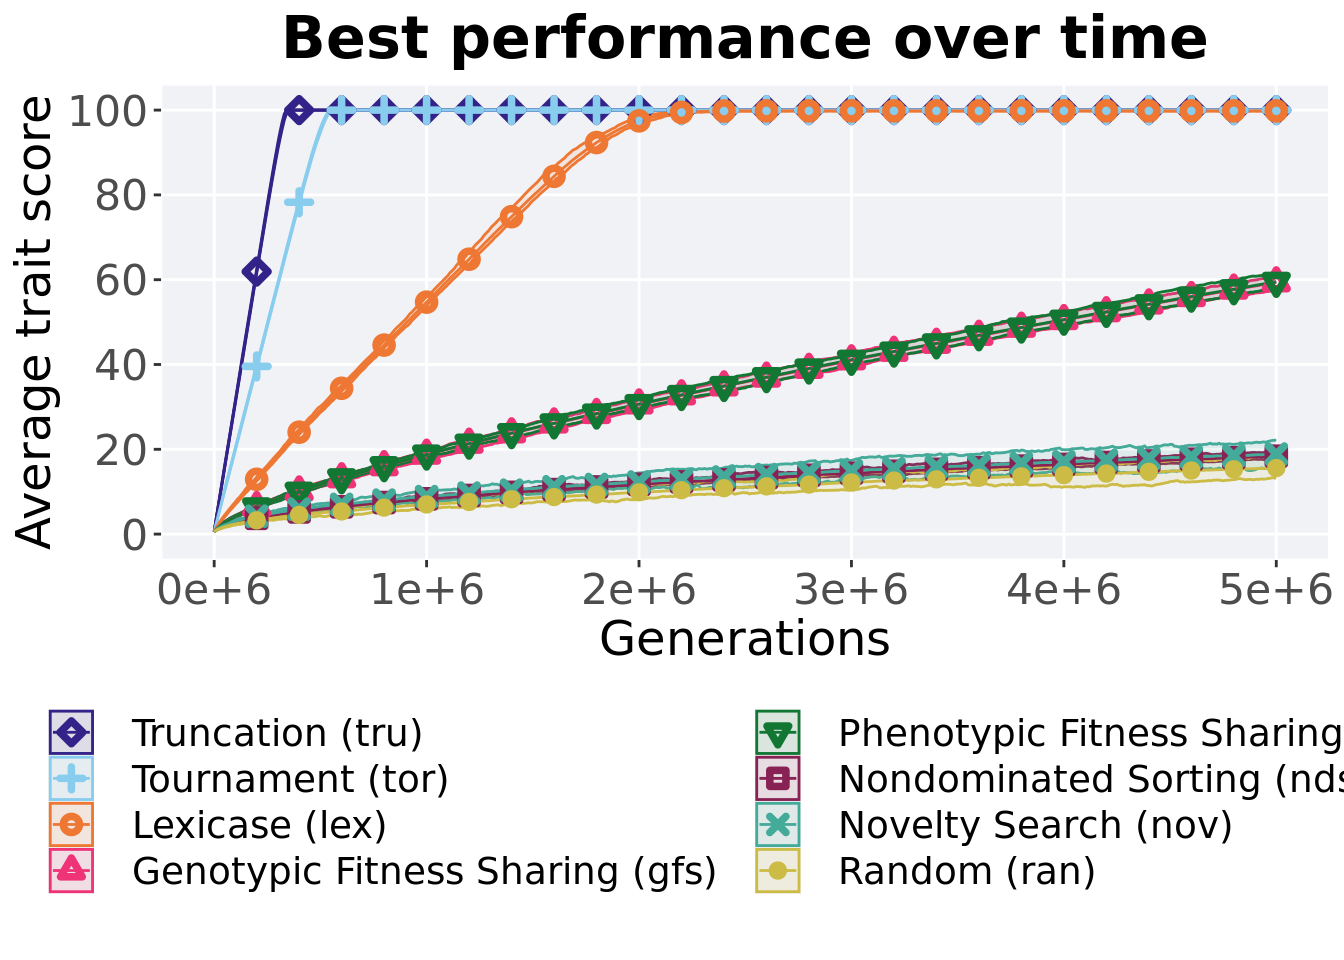
\includegraphics{demo_files/figure-latex/exp-per-ot-1.pdf}

\hypertarget{best-performance-throughout}{%
\section{Best performance throughout}\label{best-performance-throughout}}

Best performance found throughout 50,000 generations.

\begin{Shaded}
\begin{Highlighting}[]
\CommentTok{### best performance throughout}
\KeywordTok{filter}\NormalTok{(cc_best, col }\OperatorTok{==}\StringTok{ 'pop_fit_max'} \OperatorTok{&}\StringTok{ }\NormalTok{diagnostic }\OperatorTok{==}\StringTok{ 'exploitation_rate'}\NormalTok{) }\OperatorTok
\StringTok{  }\KeywordTok{ggplot}\NormalTok{(., }\KeywordTok{aes}\NormalTok{(}\DataTypeTok{x =}\NormalTok{ acron, }\DataTypeTok{y =}\NormalTok{ val }\OperatorTok{/}\StringTok{ }\NormalTok{DIMENSIONALITY, }\DataTypeTok{color =}\NormalTok{ acron, }\DataTypeTok{fill =}\NormalTok{ acron, }\DataTypeTok{shape =}\NormalTok{ acron)) }\OperatorTok{+}
\StringTok{  }\KeywordTok{geom_flat_violin}\NormalTok{(}\DataTypeTok{position =} \KeywordTok{position_nudge}\NormalTok{(}\DataTypeTok{x =} \FloatTok{.2}\NormalTok{, }\DataTypeTok{y =} \DecValTok{0}\NormalTok{), }\DataTypeTok{scale =} \StringTok{'width'}\NormalTok{, }\DataTypeTok{alpha =} \FloatTok{0.2}\NormalTok{) }\OperatorTok{+}
\StringTok{  }\KeywordTok{geom_point}\NormalTok{(}\DataTypeTok{position =} \KeywordTok{position_jitter}\NormalTok{(}\DataTypeTok{width =} \FloatTok{.1}\NormalTok{), }\DataTypeTok{size =} \FloatTok{1.5}\NormalTok{, }\DataTypeTok{alpha =} \FloatTok{1.0}\NormalTok{) }\OperatorTok{+}
\StringTok{  }\KeywordTok{geom_boxplot}\NormalTok{(}\DataTypeTok{color =} \StringTok{'black'}\NormalTok{, }\DataTypeTok{width =} \FloatTok{.2}\NormalTok{, }\DataTypeTok{outlier.shape =} \OtherTok{NA}\NormalTok{, }\DataTypeTok{alpha =} \FloatTok{0.0}\NormalTok{) }\OperatorTok{+}
\StringTok{  }\KeywordTok{scale_y_continuous}\NormalTok{(}
    \DataTypeTok{name=}\StringTok{"Average trait score"}\NormalTok{,}
    \DataTypeTok{limits=}\KeywordTok{c}\NormalTok{(}\OperatorTok{-}\DecValTok{1}\NormalTok{, }\DecValTok{101}\NormalTok{),}
    \DataTypeTok{breaks=}\KeywordTok{seq}\NormalTok{(}\DecValTok{0}\NormalTok{,}\DecValTok{100}\NormalTok{, }\DecValTok{20}\NormalTok{),}
    \DataTypeTok{labels=}\KeywordTok{c}\NormalTok{(}\StringTok{"0"}\NormalTok{, }\StringTok{"20"}\NormalTok{, }\StringTok{"40"}\NormalTok{, }\StringTok{"60"}\NormalTok{, }\StringTok{"80"}\NormalTok{, }\StringTok{"100"}\NormalTok{)}
\NormalTok{  ) }\OperatorTok{+}
\StringTok{  }\KeywordTok{scale_x_discrete}\NormalTok{(}
    \DataTypeTok{name=}\StringTok{"Scheme"}
\NormalTok{  )}\OperatorTok{+}
\StringTok{  }\KeywordTok{scale_shape_manual}\NormalTok{(}\DataTypeTok{values=}\NormalTok{SHAPE)}\OperatorTok{+}
\StringTok{  }\KeywordTok{scale_colour_manual}\NormalTok{(}\DataTypeTok{values =}\NormalTok{ cb_palette, ) }\OperatorTok{+}
\StringTok{  }\KeywordTok{scale_fill_manual}\NormalTok{(}\DataTypeTok{values =}\NormalTok{ cb_palette) }\OperatorTok{+}
\StringTok{  }\KeywordTok{ggtitle}\NormalTok{(}\StringTok{'Best performance throughout'}\NormalTok{)}\OperatorTok{+}
\StringTok{  }\NormalTok{p_theme }\OperatorTok{+}\StringTok{ }\KeywordTok{theme}\NormalTok{(}\DataTypeTok{legend.title=}\KeywordTok{element_blank}\NormalTok{()) }\OperatorTok{+}
\StringTok{  }\KeywordTok{guides}\NormalTok{(}
    \DataTypeTok{shape=}\KeywordTok{guide_legend}\NormalTok{(}\DataTypeTok{nrow=}\DecValTok{2}\NormalTok{, }\DataTypeTok{title.position =} \StringTok{"bottom"}\NormalTok{),}
    \DataTypeTok{color=}\KeywordTok{guide_legend}\NormalTok{(}\DataTypeTok{nrow=}\DecValTok{2}\NormalTok{, }\DataTypeTok{title.position =} \StringTok{"bottom"}\NormalTok{),}
    \DataTypeTok{fill=}\KeywordTok{guide_legend}\NormalTok{(}\DataTypeTok{nrow=}\DecValTok{2}\NormalTok{, }\DataTypeTok{title.position =} \StringTok{"bottom"}\NormalTok{)}
\NormalTok{  )}
\end{Highlighting}
\end{Shaded}

\begin{verbatim}
## Warning: Using the `size` aesthietic with geom_polygon was deprecated in ggplot2 3.4.0.
## i Please use the `linewidth` aesthetic instead.
\end{verbatim}

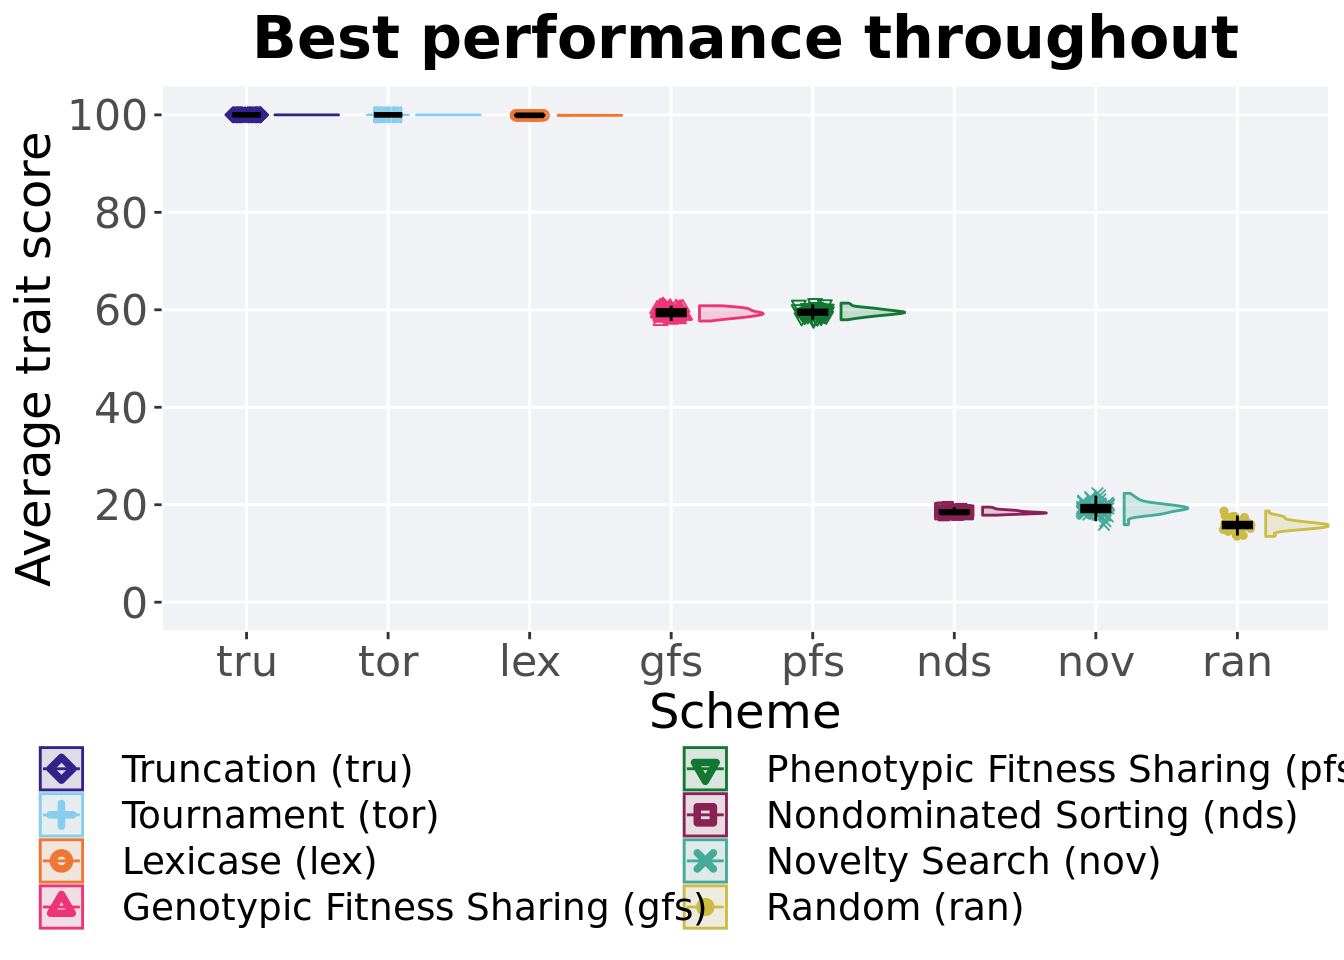
\includegraphics{demo_files/figure-latex/exp-per-bst-1.pdf}

\hypertarget{stats}{%
\subsection{Stats}\label{stats}}

Summary statistics for the best performance.

\begin{Shaded}
\begin{Highlighting}[]
\CommentTok{#get data & summarize}
\NormalTok{performance =}\StringTok{ }\KeywordTok{filter}\NormalTok{(cc_best, col }\OperatorTok{==}\StringTok{ 'pop_fit_max'} \OperatorTok{&}\StringTok{ }\NormalTok{diagnostic }\OperatorTok{==}\StringTok{ 'exploitation_rate'}\NormalTok{)}
\NormalTok{performance}\OperatorTok{$}\NormalTok{acron =}\StringTok{ }\KeywordTok{factor}\NormalTok{(performance}\OperatorTok{$}\NormalTok{acron, }\DataTypeTok{levels =} \KeywordTok{c}\NormalTok{(}\StringTok{'tru'}\NormalTok{, }\StringTok{'tor'}\NormalTok{, }\StringTok{'lex'}\NormalTok{, }\StringTok{'gfs'}\NormalTok{, }\StringTok{'pfs'}\NormalTok{, }\StringTok{'nov'}\NormalTok{, }\StringTok{'nds'}\NormalTok{, }\StringTok{'ran'}\NormalTok{))}
\NormalTok{performance }\OperatorTok
\StringTok{  }\KeywordTok{group_by}\NormalTok{(acron) }\OperatorTok
\StringTok{  }\NormalTok{dplyr}\OperatorTok{::}\KeywordTok{summarise}\NormalTok{(}
    \DataTypeTok{count =} \KeywordTok{n}\NormalTok{(),}
    \DataTypeTok{na_cnt =} \KeywordTok{sum}\NormalTok{(}\KeywordTok{is.na}\NormalTok{(val)),}
    \DataTypeTok{min =} \KeywordTok{min}\NormalTok{(val }\OperatorTok{/}\StringTok{ }\NormalTok{DIMENSIONALITY, }\DataTypeTok{na.rm =} \OtherTok{TRUE}\NormalTok{),}
    \DataTypeTok{median =} \KeywordTok{median}\NormalTok{(val }\OperatorTok{/}\StringTok{ }\NormalTok{DIMENSIONALITY, }\DataTypeTok{na.rm =} \OtherTok{TRUE}\NormalTok{),}
    \DataTypeTok{mean =} \KeywordTok{mean}\NormalTok{(val }\OperatorTok{/}\StringTok{ }\NormalTok{DIMENSIONALITY, }\DataTypeTok{na.rm =} \OtherTok{TRUE}\NormalTok{),}
    \DataTypeTok{max =} \KeywordTok{max}\NormalTok{(val }\OperatorTok{/}\StringTok{ }\NormalTok{DIMENSIONALITY, }\DataTypeTok{na.rm =} \OtherTok{TRUE}\NormalTok{),}
    \DataTypeTok{IQR =} \KeywordTok{IQR}\NormalTok{(val }\OperatorTok{/}\StringTok{ }\NormalTok{DIMENSIONALITY, }\DataTypeTok{na.rm =} \OtherTok{TRUE}\NormalTok{)}
\NormalTok{  )}
\end{Highlighting}
\end{Shaded}

\begin{verbatim}
## # A tibble: 8 x 8
##   acron count na_cnt   min median  mean   max    IQR
##   <fct> <int>  <int> <dbl>  <dbl> <dbl> <dbl>  <dbl>
## 1 tru      50      0 100    100   100   100   0     
## 2 tor      50      0 100    100   100   100   0     
## 3 lex      50      0  99.9   99.9  99.9  99.9 0.0137
## 4 gfs      50      0  57.7   59.3  59.4  60.8 1.31  
## 5 pfs      50      0  58.0   59.5  59.5  61.4 0.908 
## 6 nov      50      0  15.9   19.2  19.3  22.3 1.34  
## 7 nds      50      0  17.9   18.4  18.5  19.5 0.516 
## 8 ran      50      0  13.5   15.9  15.9  18.7 1.15
\end{verbatim}

Kruskal--Wallis test provides evidence of statistical differences.

\begin{Shaded}
\begin{Highlighting}[]
\KeywordTok{kruskal.test}\NormalTok{(val }\OperatorTok{~}\StringTok{ }\NormalTok{acron, }\DataTypeTok{data =}\NormalTok{ performance)}
\end{Highlighting}
\end{Shaded}

\begin{verbatim}
## 
##  Kruskal-Wallis rank sum test
## 
## data:  val by acron
## Kruskal-Wallis chi-squared = 384.91, df = 7, p-value < 2.2e-16
\end{verbatim}

Results for post-hoc Wilcoxon rank-sum test with a Bonferroni correction.

\begin{Shaded}
\begin{Highlighting}[]
\KeywordTok{pairwise.wilcox.test}\NormalTok{(}\DataTypeTok{x =}\NormalTok{ performance}\OperatorTok{$}\NormalTok{val, }\DataTypeTok{g =}\NormalTok{ performance}\OperatorTok{$}\NormalTok{acron, }\DataTypeTok{p.adjust.method =} \StringTok{"bonferroni"}\NormalTok{,}
                     \DataTypeTok{paired =} \OtherTok{FALSE}\NormalTok{, }\DataTypeTok{conf.int =} \OtherTok{FALSE}\NormalTok{, }\DataTypeTok{alternative =} \StringTok{'l'}\NormalTok{)}
\end{Highlighting}
\end{Shaded}

\begin{verbatim}
## 
##  Pairwise comparisons using Wilcoxon rank sum test with continuity correction 
## 
## data:  performance$val and performance$acron 
## 
##     tru     tor     lex     gfs     pfs     nov     nds    
## tor 1e+00   -       -       -       -       -       -      
## lex < 2e-16 < 2e-16 -       -       -       -       -      
## gfs < 2e-16 < 2e-16 < 2e-16 -       -       -       -      
## pfs < 2e-16 < 2e-16 < 2e-16 1e+00   -       -       -      
## nov < 2e-16 < 2e-16 < 2e-16 < 2e-16 < 2e-16 -       -      
## nds < 2e-16 < 2e-16 < 2e-16 < 2e-16 < 2e-16 6e-04   -      
## ran < 2e-16 < 2e-16 < 2e-16 < 2e-16 < 2e-16 1.9e-15 7.9e-16
## 
## P value adjustment method: bonferroni
\end{verbatim}

\hypertarget{generation-satisfactory-solution-found}{%
\section{Generation satisfactory solution found}\label{generation-satisfactory-solution-found}}

First generation a satisfactory solution is found throughout the 50,000 generations.

\begin{Shaded}
\begin{Highlighting}[]
\KeywordTok{filter}\NormalTok{(cc_ssf, diagnostic }\OperatorTok{==}\StringTok{ 'exploitation_rate'}\NormalTok{) }\OperatorTok
\StringTok{  }\KeywordTok{ggplot}\NormalTok{(., }\KeywordTok{aes}\NormalTok{(}\DataTypeTok{x =}\NormalTok{ acron, }\DataTypeTok{y =}\NormalTok{ Generations , }\DataTypeTok{color =}\NormalTok{ acron, }\DataTypeTok{fill =}\NormalTok{ acron, }\DataTypeTok{shape =}\NormalTok{ acron)) }\OperatorTok{+}
\StringTok{  }\KeywordTok{geom_flat_violin}\NormalTok{(}\DataTypeTok{position =} \KeywordTok{position_nudge}\NormalTok{(}\DataTypeTok{x =} \FloatTok{.2}\NormalTok{, }\DataTypeTok{y =} \DecValTok{0}\NormalTok{), }\DataTypeTok{scale =} \StringTok{'width'}\NormalTok{, }\DataTypeTok{alpha =} \FloatTok{0.2}\NormalTok{) }\OperatorTok{+}
\StringTok{  }\KeywordTok{geom_point}\NormalTok{(}\DataTypeTok{position =} \KeywordTok{position_jitter}\NormalTok{(}\DataTypeTok{width =} \FloatTok{.1}\NormalTok{), }\DataTypeTok{size =} \FloatTok{1.5}\NormalTok{, }\DataTypeTok{alpha =} \FloatTok{1.0}\NormalTok{) }\OperatorTok{+}
\StringTok{  }\KeywordTok{geom_boxplot}\NormalTok{(}\DataTypeTok{color =} \StringTok{'black'}\NormalTok{, }\DataTypeTok{width =} \FloatTok{.2}\NormalTok{, }\DataTypeTok{outlier.shape =} \OtherTok{NA}\NormalTok{, }\DataTypeTok{alpha =} \FloatTok{0.0}\NormalTok{) }\OperatorTok{+}
\StringTok{  }\KeywordTok{scale_y_continuous}\NormalTok{(}
    \DataTypeTok{name=}\StringTok{"Generation"}\NormalTok{,}
    \DataTypeTok{limits=}\KeywordTok{c}\NormalTok{(}\DecValTok{0}\NormalTok{, }\DecValTok{60001}\NormalTok{),}
    \DataTypeTok{breaks=}\KeywordTok{c}\NormalTok{(}\DecValTok{0}\NormalTok{, }\DecValTok{10000}\NormalTok{, }\DecValTok{20000}\NormalTok{, }\DecValTok{30000}\NormalTok{, }\DecValTok{40000}\NormalTok{, }\DecValTok{50000}\NormalTok{, }\DecValTok{60000}\NormalTok{),}
    \DataTypeTok{labels=}\KeywordTok{c}\NormalTok{(}\StringTok{"0e+4"}\NormalTok{, }\StringTok{"1e+4"}\NormalTok{, }\StringTok{"2e+4"}\NormalTok{, }\StringTok{"3e+4"}\NormalTok{, }\StringTok{"4e+4"}\NormalTok{, }\StringTok{"5e+4"}\NormalTok{, }\StringTok{"Fail"}\NormalTok{)}
\NormalTok{  ) }\OperatorTok{+}
\StringTok{  }\KeywordTok{scale_x_discrete}\NormalTok{(}
    \DataTypeTok{name=}\StringTok{"Scheme"}
\NormalTok{  )}\OperatorTok{+}
\StringTok{  }\KeywordTok{scale_shape_manual}\NormalTok{(}\DataTypeTok{values=}\NormalTok{SHAPE)}\OperatorTok{+}
\StringTok{  }\KeywordTok{scale_colour_manual}\NormalTok{(}\DataTypeTok{values =}\NormalTok{ cb_palette, ) }\OperatorTok{+}
\StringTok{  }\KeywordTok{scale_fill_manual}\NormalTok{(}\DataTypeTok{values =}\NormalTok{ cb_palette) }\OperatorTok{+}
\StringTok{  }\KeywordTok{ggtitle}\NormalTok{(}\StringTok{'Generation satisfactory solution found'}\NormalTok{)}\OperatorTok{+}
\StringTok{  }\NormalTok{p_theme }\OperatorTok{+}\StringTok{ }\KeywordTok{theme}\NormalTok{(}\DataTypeTok{legend.title=}\KeywordTok{element_blank}\NormalTok{()) }\OperatorTok{+}
\StringTok{  }\KeywordTok{guides}\NormalTok{(}
    \DataTypeTok{shape=}\KeywordTok{guide_legend}\NormalTok{(}\DataTypeTok{nrow=}\DecValTok{2}\NormalTok{, }\DataTypeTok{title.position =} \StringTok{"bottom"}\NormalTok{),}
    \DataTypeTok{color=}\KeywordTok{guide_legend}\NormalTok{(}\DataTypeTok{nrow=}\DecValTok{2}\NormalTok{, }\DataTypeTok{title.position =} \StringTok{"bottom"}\NormalTok{),}
    \DataTypeTok{fill=}\KeywordTok{guide_legend}\NormalTok{(}\DataTypeTok{nrow=}\DecValTok{2}\NormalTok{, }\DataTypeTok{title.position =} \StringTok{"bottom"}\NormalTok{)}
\NormalTok{  )}
\end{Highlighting}
\end{Shaded}

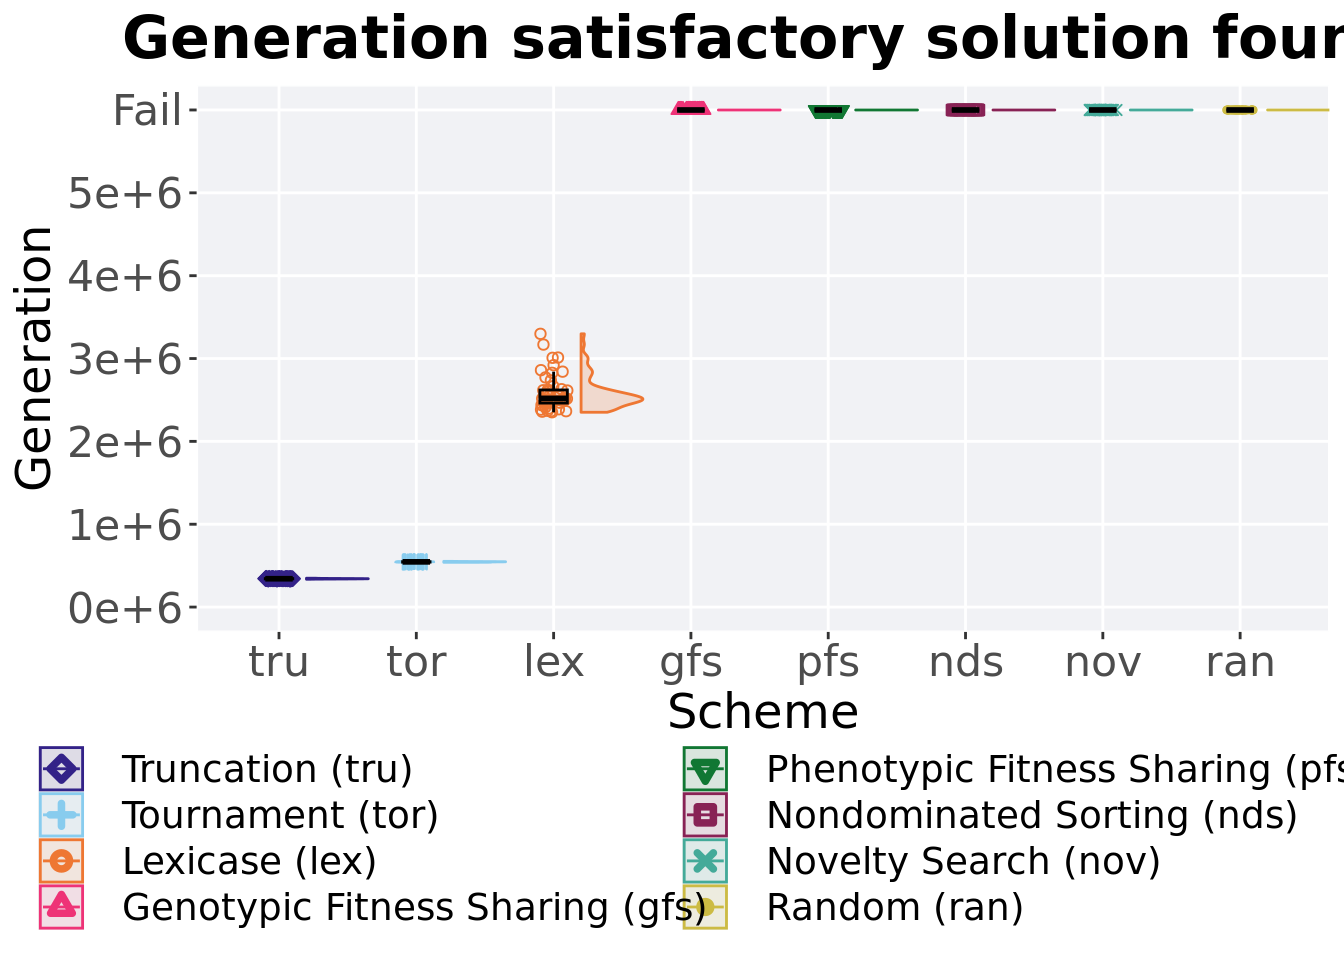
\includegraphics{demo_files/figure-latex/exp-ssf-1.pdf}

\hypertarget{stats-1}{%
\subsection{Stats}\label{stats-1}}

Summary statistics for the first generation a satisfactory solution is found.

\begin{Shaded}
\begin{Highlighting}[]
\NormalTok{ssf =}\StringTok{ }\KeywordTok{filter}\NormalTok{(cc_ssf, diagnostic }\OperatorTok{==}\StringTok{ 'exploitation_rate'}  \OperatorTok{&}\StringTok{ }\NormalTok{Generations }\OperatorTok{<}\StringTok{ }\DecValTok{60000}\NormalTok{)}
\NormalTok{ssf}\OperatorTok{$}\NormalTok{acron =}\StringTok{ }\KeywordTok{factor}\NormalTok{(ssf}\OperatorTok{$}\NormalTok{acron, }\DataTypeTok{levels =} \KeywordTok{c}\NormalTok{(}\StringTok{'tru'}\NormalTok{, }\StringTok{'tor'}\NormalTok{, }\StringTok{'lex'}\NormalTok{))}
\NormalTok{ssf }\OperatorTok
\StringTok{  }\KeywordTok{group_by}\NormalTok{(acron) }\OperatorTok
\StringTok{  }\NormalTok{dplyr}\OperatorTok{::}\KeywordTok{summarise}\NormalTok{(}
    \DataTypeTok{count =} \KeywordTok{n}\NormalTok{(),}
    \DataTypeTok{na_cnt =} \KeywordTok{sum}\NormalTok{(}\KeywordTok{is.na}\NormalTok{(Generations)),}
    \DataTypeTok{min =} \KeywordTok{min}\NormalTok{(Generations, }\DataTypeTok{na.rm =} \OtherTok{TRUE}\NormalTok{),}
    \DataTypeTok{median =} \KeywordTok{median}\NormalTok{(Generations, }\DataTypeTok{na.rm =} \OtherTok{TRUE}\NormalTok{),}
    \DataTypeTok{mean =} \KeywordTok{mean}\NormalTok{(Generations, }\DataTypeTok{na.rm =} \OtherTok{TRUE}\NormalTok{),}
    \DataTypeTok{max =} \KeywordTok{max}\NormalTok{(Generations, }\DataTypeTok{na.rm =} \OtherTok{TRUE}\NormalTok{),}
    \DataTypeTok{IQR =} \KeywordTok{IQR}\NormalTok{(Generations, }\DataTypeTok{na.rm =} \OtherTok{TRUE}\NormalTok{)}
\NormalTok{  )}
\end{Highlighting}
\end{Shaded}

\begin{verbatim}
## # A tibble: 3 x 8
##   acron count na_cnt   min median   mean   max    IQR
##   <fct> <int>  <int> <int>  <dbl>  <dbl> <int>  <dbl>
## 1 tru      50      0  3357   3420  3421.  3481   34.2
## 2 tor      50      0  5403   5457  5453.  5519   51.8
## 3 lex      50      0 23514  25190 25857. 32980 1581
\end{verbatim}

Kruskal--Wallis test provides evidence of difference amoung selection schemes.

\begin{Shaded}
\begin{Highlighting}[]
\KeywordTok{kruskal.test}\NormalTok{(Generations }\OperatorTok{~}\StringTok{ }\NormalTok{acron, }\DataTypeTok{data =}\NormalTok{ ssf)}
\end{Highlighting}
\end{Shaded}

\begin{verbatim}
## 
##  Kruskal-Wallis rank sum test
## 
## data:  Generations by acron
## Kruskal-Wallis chi-squared = 132.46, df = 2, p-value < 2.2e-16
\end{verbatim}

Results for post-hoc Wilcoxon rank-sum test with a Bonferroni correction.

\begin{Shaded}
\begin{Highlighting}[]
\KeywordTok{pairwise.wilcox.test}\NormalTok{(}\DataTypeTok{x =}\NormalTok{ ssf}\OperatorTok{$}\NormalTok{Generations, }\DataTypeTok{g =}\NormalTok{ ssf}\OperatorTok{$}\NormalTok{acron, }\DataTypeTok{p.adjust.method =} \StringTok{"bonferroni"}\NormalTok{,}
                     \DataTypeTok{paired =} \OtherTok{FALSE}\NormalTok{, }\DataTypeTok{conf.int =} \OtherTok{FALSE}\NormalTok{, }\DataTypeTok{alternative =} \StringTok{'g'}\NormalTok{)}
\end{Highlighting}
\end{Shaded}

\begin{verbatim}
## 
##  Pairwise comparisons using Wilcoxon rank sum test with continuity correction 
## 
## data:  ssf$Generations and ssf$acron 
## 
##     tru    tor   
## tor <2e-16 -     
## lex <2e-16 <2e-16
## 
## P value adjustment method: bonferroni
\end{verbatim}

\hypertarget{multi-valley-crossing-results}{%
\section{Multi-valley crossing results}\label{multi-valley-crossing-results}}

\hypertarget{performance-over-time-1}{%
\subsection{Performance over time}\label{performance-over-time-1}}

Best performance in a population over time.

\begin{Shaded}
\begin{Highlighting}[]
\CommentTok{# data for lines and shading on plots}
\NormalTok{lines =}\StringTok{ }\KeywordTok{filter}\NormalTok{(cc_over_time_mvc, diagnostic }\OperatorTok{==}\StringTok{ 'exploitation_rate'}\NormalTok{) }\OperatorTok
\StringTok{  }\KeywordTok{group_by}\NormalTok{(}\StringTok{`}\DataTypeTok{Selection}\CharTok{\textbackslash{}n}\DataTypeTok{Scheme}\StringTok{`}\NormalTok{, gen) }\OperatorTok
\StringTok{  }\NormalTok{dplyr}\OperatorTok{::}\KeywordTok{summarise}\NormalTok{(}
    \DataTypeTok{min =} \KeywordTok{min}\NormalTok{(pop_fit_max) }\OperatorTok{/}\StringTok{ }\NormalTok{DIMENSIONALITY,}
    \DataTypeTok{mean =} \KeywordTok{mean}\NormalTok{(pop_fit_max) }\OperatorTok{/}\StringTok{ }\NormalTok{DIMENSIONALITY,}
    \DataTypeTok{max =} \KeywordTok{max}\NormalTok{(pop_fit_max) }\OperatorTok{/}\StringTok{ }\NormalTok{DIMENSIONALITY}
\NormalTok{  )}
\end{Highlighting}
\end{Shaded}

\begin{verbatim}
## `summarise()` has grouped output by 'Selection Scheme'. You can override using
## the `.groups` argument.
\end{verbatim}

\begin{Shaded}
\begin{Highlighting}[]
\KeywordTok{ggplot}\NormalTok{(lines, }\KeywordTok{aes}\NormalTok{(}\DataTypeTok{x=}\NormalTok{gen, }\DataTypeTok{y=}\NormalTok{mean, }\DataTypeTok{group =} \StringTok{`}\DataTypeTok{Selection}\CharTok{\textbackslash{}n}\DataTypeTok{Scheme}\StringTok{`}\NormalTok{, }\DataTypeTok{fill =}\StringTok{`}\DataTypeTok{Selection}\CharTok{\textbackslash{}n}\DataTypeTok{Scheme}\StringTok{`}\NormalTok{, }\DataTypeTok{color =} \StringTok{`}\DataTypeTok{Selection}\CharTok{\textbackslash{}n}\DataTypeTok{Scheme}\StringTok{`}\NormalTok{, }\DataTypeTok{shape =} \StringTok{`}\DataTypeTok{Selection}\CharTok{\textbackslash{}n}\DataTypeTok{Scheme}\StringTok{`}\NormalTok{)) }\OperatorTok{+}
\StringTok{  }\KeywordTok{geom_ribbon}\NormalTok{(}\KeywordTok{aes}\NormalTok{(}\DataTypeTok{ymin =}\NormalTok{ min, }\DataTypeTok{ymax =}\NormalTok{ max), }\DataTypeTok{alpha =} \FloatTok{0.1}\NormalTok{) }\OperatorTok{+}
\StringTok{  }\KeywordTok{geom_line}\NormalTok{(}\DataTypeTok{size =} \FloatTok{0.5}\NormalTok{) }\OperatorTok{+}
\StringTok{  }\KeywordTok{geom_point}\NormalTok{(}\DataTypeTok{data =} \KeywordTok{filter}\NormalTok{(lines, gen }\OperatorTok\StringTok{ }\DecValTok{2000} \OperatorTok{==}\StringTok{ }\DecValTok{0} \OperatorTok{&}\StringTok{ }\NormalTok{gen }\OperatorTok{!=}\StringTok{ }\DecValTok{0}\NormalTok{), }\DataTypeTok{size =} \FloatTok{1.5}\NormalTok{, }\DataTypeTok{stroke =} \FloatTok{2.0}\NormalTok{, }\DataTypeTok{alpha =} \FloatTok{1.0}\NormalTok{) }\OperatorTok{+}
\StringTok{  }\KeywordTok{scale_y_continuous}\NormalTok{(}
    \DataTypeTok{name=}\StringTok{"Average trait score"}\NormalTok{,}
    \DataTypeTok{limits=}\KeywordTok{c}\NormalTok{(}\DecValTok{0}\NormalTok{, }\DecValTok{50}\NormalTok{),}
    \DataTypeTok{breaks=}\KeywordTok{seq}\NormalTok{(}\DecValTok{0}\NormalTok{,}\DecValTok{50}\NormalTok{, }\DecValTok{10}\NormalTok{),}
    \DataTypeTok{labels=}\KeywordTok{c}\NormalTok{(}\StringTok{"0"}\NormalTok{, }\StringTok{"10"}\NormalTok{, }\StringTok{"20"}\NormalTok{, }\StringTok{"30"}\NormalTok{, }\StringTok{"40"}\NormalTok{, }\StringTok{"50"}\NormalTok{)}
\NormalTok{  ) }\OperatorTok{+}
\StringTok{  }\KeywordTok{scale_x_continuous}\NormalTok{(}
    \DataTypeTok{name=}\StringTok{"Generations"}\NormalTok{,}
    \DataTypeTok{limits=}\KeywordTok{c}\NormalTok{(}\DecValTok{0}\NormalTok{, }\DecValTok{50000}\NormalTok{),}
    \DataTypeTok{breaks=}\KeywordTok{c}\NormalTok{(}\DecValTok{0}\NormalTok{, }\DecValTok{10000}\NormalTok{, }\DecValTok{20000}\NormalTok{, }\DecValTok{30000}\NormalTok{, }\DecValTok{40000}\NormalTok{, }\DecValTok{50000}\NormalTok{),}
    \DataTypeTok{labels=}\KeywordTok{c}\NormalTok{(}\StringTok{"0e+4"}\NormalTok{, }\StringTok{"1e+4"}\NormalTok{, }\StringTok{"2e+4"}\NormalTok{, }\StringTok{"3e+4"}\NormalTok{, }\StringTok{"4e+4"}\NormalTok{, }\StringTok{"5e+4"}\NormalTok{)}

\NormalTok{  ) }\OperatorTok{+}
\StringTok{  }\KeywordTok{scale_shape_manual}\NormalTok{(}\DataTypeTok{values=}\NormalTok{SHAPE)}\OperatorTok{+}
\StringTok{  }\KeywordTok{scale_colour_manual}\NormalTok{(}\DataTypeTok{values =}\NormalTok{ cb_palette) }\OperatorTok{+}
\StringTok{  }\KeywordTok{scale_fill_manual}\NormalTok{(}\DataTypeTok{values =}\NormalTok{ cb_palette) }\OperatorTok{+}
\StringTok{  }\KeywordTok{ggtitle}\NormalTok{(}\StringTok{'Performance over time'}\NormalTok{)}\OperatorTok{+}
\StringTok{  }\NormalTok{p_theme }\OperatorTok{+}\StringTok{ }\KeywordTok{theme}\NormalTok{(}\DataTypeTok{legend.title=}\KeywordTok{element_blank}\NormalTok{(),}\DataTypeTok{legend.text=}\KeywordTok{element_text}\NormalTok{(}\DataTypeTok{size=}\DecValTok{11}\NormalTok{)) }\OperatorTok{+}
\StringTok{  }\KeywordTok{guides}\NormalTok{(}
    \DataTypeTok{sh=}\KeywordTok{guide_legend}\NormalTok{(}\DataTypeTok{ncol=}\DecValTok{2}\NormalTok{, }\DataTypeTok{title.position =} \StringTok{"left"}\NormalTok{),}
    \DataTypeTok{color=}\KeywordTok{guide_legend}\NormalTok{(}\DataTypeTok{ncol=}\DecValTok{2}\NormalTok{, }\DataTypeTok{title.position =} \StringTok{"left"}\NormalTok{),}
    \DataTypeTok{fillape=}\KeywordTok{guide_legend}\NormalTok{(}\DataTypeTok{ncol=}\DecValTok{2}\NormalTok{, }\DataTypeTok{title.position =} \StringTok{"left"}\NormalTok{)}
\NormalTok{  )}
\end{Highlighting}
\end{Shaded}

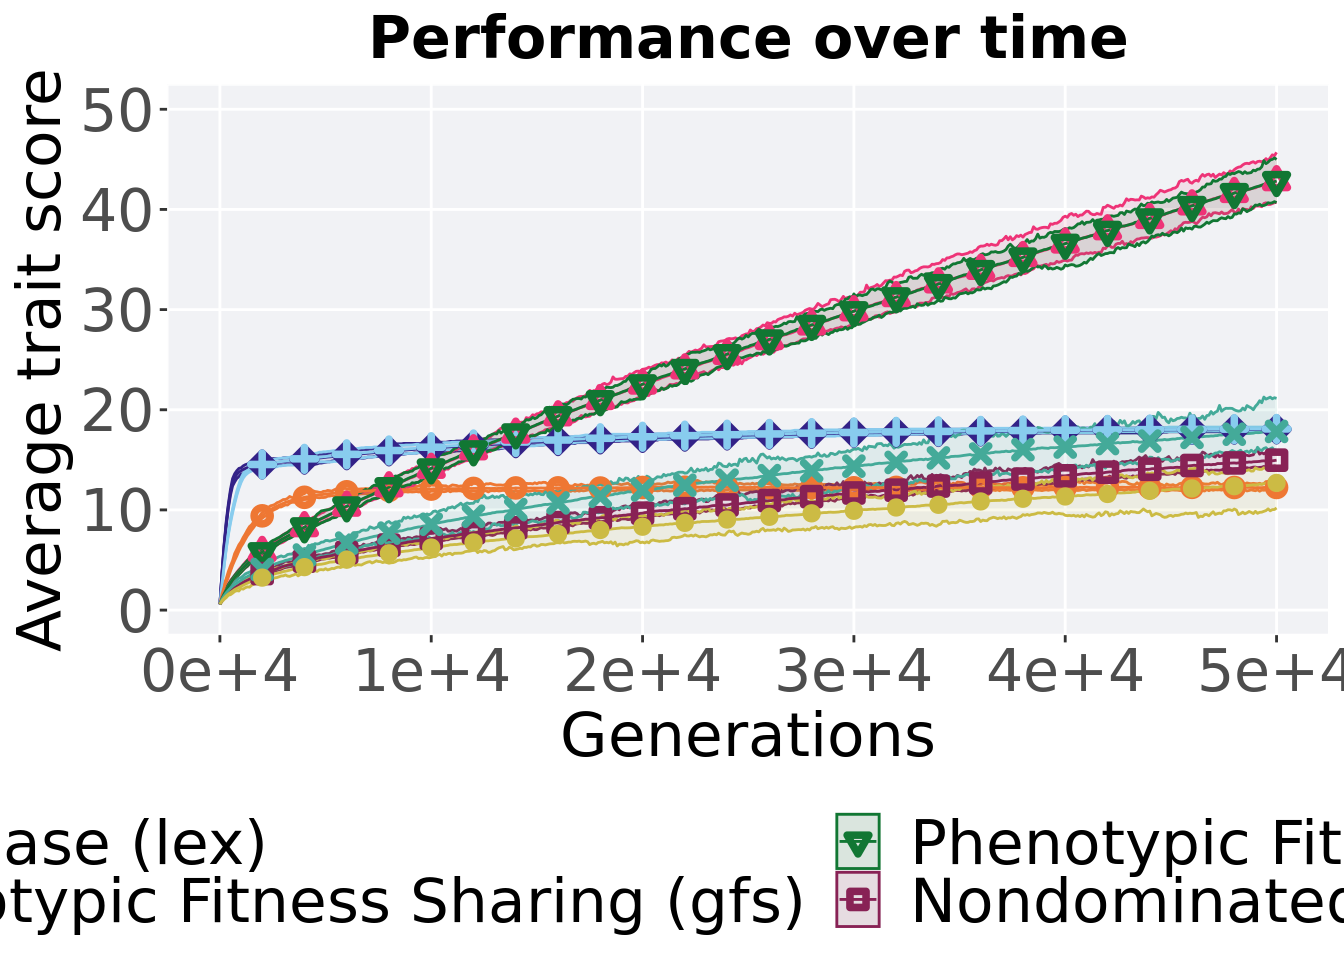
\includegraphics{demo_files/figure-latex/exp-mvc-per-ot-1.pdf}

\hypertarget{best-performance-throughout-1}{%
\subsection{Best performance throughout}\label{best-performance-throughout-1}}

Best performance found throughout 50,000 generations.

\begin{Shaded}
\begin{Highlighting}[]
\CommentTok{### best performance throughout}
\KeywordTok{filter}\NormalTok{(cc_best_mvc, col }\OperatorTok{==}\StringTok{ 'pop_fit_max'} \OperatorTok{&}\StringTok{ }\NormalTok{diagnostic }\OperatorTok{==}\StringTok{ 'exploitation_rate'}\NormalTok{) }\OperatorTok
\StringTok{  }\KeywordTok{ggplot}\NormalTok{(., }\KeywordTok{aes}\NormalTok{(}\DataTypeTok{x =}\NormalTok{ acron, }\DataTypeTok{y =}\NormalTok{ val }\OperatorTok{/}\StringTok{ }\NormalTok{DIMENSIONALITY, }\DataTypeTok{color =}\NormalTok{ acron, }\DataTypeTok{fill =}\NormalTok{ acron, }\DataTypeTok{shape =}\NormalTok{ acron)) }\OperatorTok{+}
\StringTok{  }\KeywordTok{geom_flat_violin}\NormalTok{(}\DataTypeTok{position =} \KeywordTok{position_nudge}\NormalTok{(}\DataTypeTok{x =} \FloatTok{.2}\NormalTok{, }\DataTypeTok{y =} \DecValTok{0}\NormalTok{), }\DataTypeTok{scale =} \StringTok{'width'}\NormalTok{, }\DataTypeTok{alpha =} \FloatTok{0.2}\NormalTok{) }\OperatorTok{+}
\StringTok{  }\KeywordTok{geom_point}\NormalTok{(}\DataTypeTok{position =} \KeywordTok{position_jitter}\NormalTok{(}\DataTypeTok{width =} \FloatTok{.1}\NormalTok{), }\DataTypeTok{size =} \FloatTok{1.5}\NormalTok{, }\DataTypeTok{alpha =} \FloatTok{1.0}\NormalTok{) }\OperatorTok{+}
\StringTok{  }\KeywordTok{geom_boxplot}\NormalTok{(}\DataTypeTok{color =} \StringTok{'black'}\NormalTok{, }\DataTypeTok{width =} \FloatTok{.2}\NormalTok{, }\DataTypeTok{outlier.shape =} \OtherTok{NA}\NormalTok{, }\DataTypeTok{alpha =} \FloatTok{0.0}\NormalTok{) }\OperatorTok{+}
\StringTok{  }\KeywordTok{scale_y_continuous}\NormalTok{(}
    \DataTypeTok{name=}\StringTok{"Average trait score"}\NormalTok{,}
    \DataTypeTok{limits=}\KeywordTok{c}\NormalTok{(}\DecValTok{0}\NormalTok{, }\DecValTok{50}\NormalTok{),}
    \DataTypeTok{breaks=}\KeywordTok{seq}\NormalTok{(}\DecValTok{0}\NormalTok{,}\DecValTok{50}\NormalTok{, }\DecValTok{10}\NormalTok{),}
    \DataTypeTok{labels=}\KeywordTok{c}\NormalTok{(}\StringTok{"0"}\NormalTok{, }\StringTok{"10"}\NormalTok{, }\StringTok{"20"}\NormalTok{, }\StringTok{"30"}\NormalTok{, }\StringTok{"40"}\NormalTok{, }\StringTok{"50"}\NormalTok{)}
\NormalTok{  ) }\OperatorTok{+}
\StringTok{  }\KeywordTok{scale_x_discrete}\NormalTok{(}
    \DataTypeTok{name=}\StringTok{"Scheme"}
\NormalTok{  )}\OperatorTok{+}
\StringTok{  }\KeywordTok{scale_shape_manual}\NormalTok{(}\DataTypeTok{values=}\NormalTok{SHAPE)}\OperatorTok{+}
\StringTok{  }\KeywordTok{scale_colour_manual}\NormalTok{(}\DataTypeTok{values =}\NormalTok{ cb_palette, ) }\OperatorTok{+}
\StringTok{  }\KeywordTok{scale_fill_manual}\NormalTok{(}\DataTypeTok{values =}\NormalTok{ cb_palette) }\OperatorTok{+}
\StringTok{  }\KeywordTok{ggtitle}\NormalTok{(}\StringTok{'Best performance throughout'}\NormalTok{)}\OperatorTok{+}
\StringTok{  }\NormalTok{p_theme }\OperatorTok{+}\StringTok{ }\KeywordTok{theme}\NormalTok{(}\DataTypeTok{legend.title=}\KeywordTok{element_blank}\NormalTok{()) }\OperatorTok{+}
\StringTok{  }\KeywordTok{guides}\NormalTok{(}
    \DataTypeTok{shape=}\KeywordTok{guide_legend}\NormalTok{(}\DataTypeTok{nrow=}\DecValTok{2}\NormalTok{, }\DataTypeTok{title.position =} \StringTok{"bottom"}\NormalTok{),}
    \DataTypeTok{color=}\KeywordTok{guide_legend}\NormalTok{(}\DataTypeTok{nrow=}\DecValTok{2}\NormalTok{, }\DataTypeTok{title.position =} \StringTok{"bottom"}\NormalTok{),}
    \DataTypeTok{fill=}\KeywordTok{guide_legend}\NormalTok{(}\DataTypeTok{nrow=}\DecValTok{2}\NormalTok{, }\DataTypeTok{title.position =} \StringTok{"bottom"}\NormalTok{)}
\NormalTok{  )}
\end{Highlighting}
\end{Shaded}

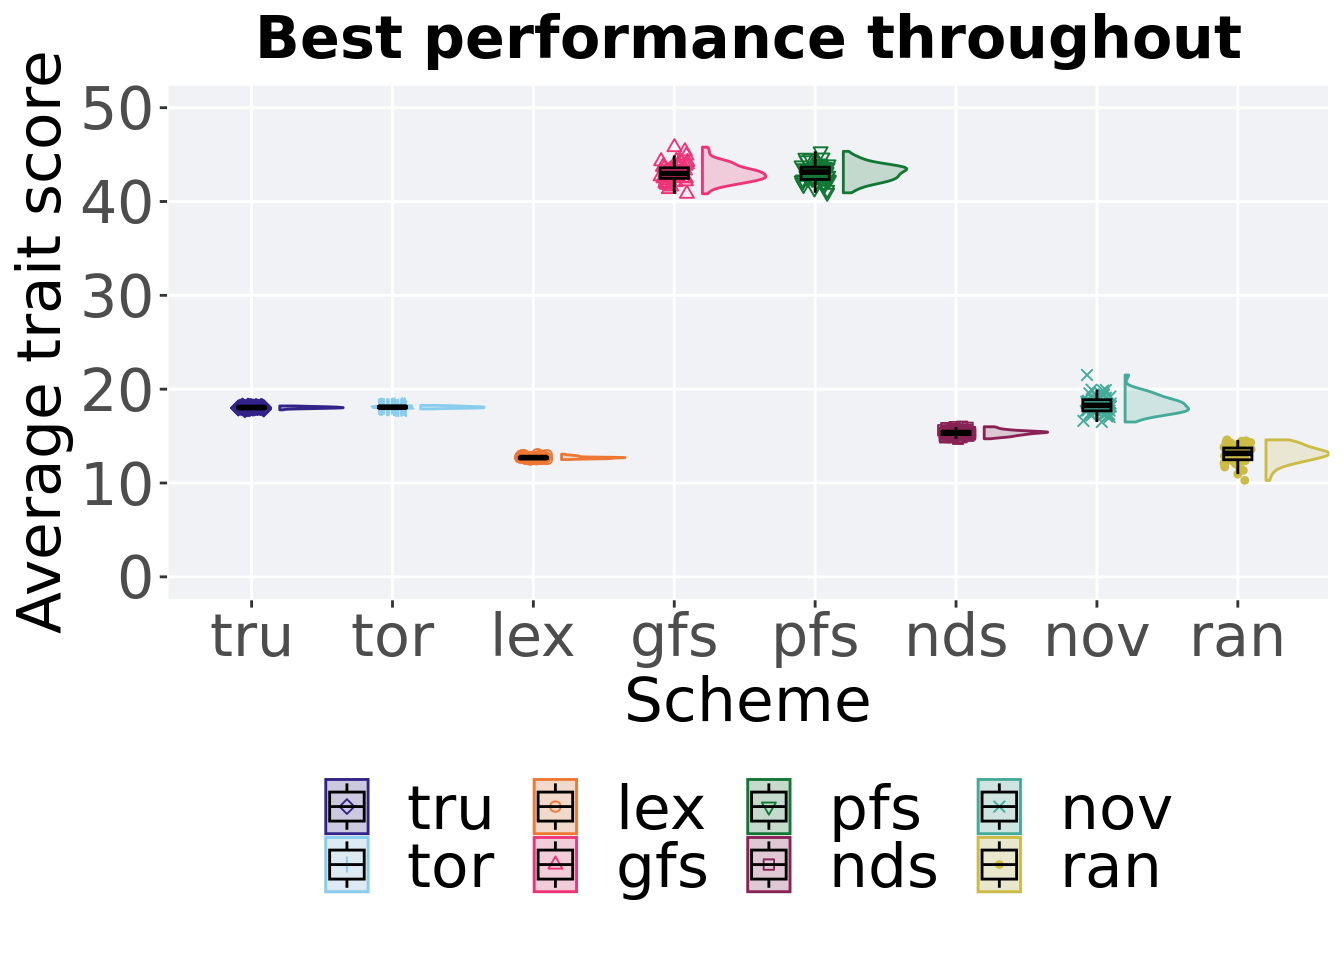
\includegraphics{demo_files/figure-latex/exp-mvc-per-bst-1.pdf}

\hypertarget{stats-2}{%
\subsubsection{Stats}\label{stats-2}}

Summary statistics for the performance of the best performance.

\begin{Shaded}
\begin{Highlighting}[]
\CommentTok{#get data & summarize}
\NormalTok{performance =}\StringTok{ }\KeywordTok{filter}\NormalTok{(cc_best_mvc, col }\OperatorTok{==}\StringTok{ 'pop_fit_max'} \OperatorTok{&}\StringTok{ }\NormalTok{diagnostic }\OperatorTok{==}\StringTok{ 'exploitation_rate'}\NormalTok{)}
\NormalTok{performance}\OperatorTok{$}\NormalTok{acron =}\StringTok{ }\KeywordTok{factor}\NormalTok{(performance}\OperatorTok{$}\NormalTok{acron, }\DataTypeTok{levels =} \KeywordTok{c}\NormalTok{(}\StringTok{'gfs'}\NormalTok{,}\StringTok{'pfs'}\NormalTok{,}\StringTok{'tru'}\NormalTok{,}\StringTok{'tor'}\NormalTok{,}\StringTok{'nov'}\NormalTok{, }\StringTok{'nds'}\NormalTok{,}\StringTok{'lex'}\NormalTok{, }\StringTok{'ran'}\NormalTok{))}
\NormalTok{performance }\OperatorTok
\StringTok{  }\KeywordTok{group_by}\NormalTok{(acron) }\OperatorTok
\StringTok{  }\NormalTok{dplyr}\OperatorTok{::}\KeywordTok{summarise}\NormalTok{(}
    \DataTypeTok{count =} \KeywordTok{n}\NormalTok{(),}
    \DataTypeTok{na_cnt =} \KeywordTok{sum}\NormalTok{(}\KeywordTok{is.na}\NormalTok{(val)),}
    \DataTypeTok{min =} \KeywordTok{min}\NormalTok{(val }\OperatorTok{/}\StringTok{ }\NormalTok{DIMENSIONALITY, }\DataTypeTok{na.rm =} \OtherTok{TRUE}\NormalTok{),}
    \DataTypeTok{median =} \KeywordTok{median}\NormalTok{(val }\OperatorTok{/}\StringTok{ }\NormalTok{DIMENSIONALITY, }\DataTypeTok{na.rm =} \OtherTok{TRUE}\NormalTok{),}
    \DataTypeTok{mean =} \KeywordTok{mean}\NormalTok{(val }\OperatorTok{/}\StringTok{ }\NormalTok{DIMENSIONALITY, }\DataTypeTok{na.rm =} \OtherTok{TRUE}\NormalTok{),}
    \DataTypeTok{max =} \KeywordTok{max}\NormalTok{(val }\OperatorTok{/}\StringTok{ }\NormalTok{DIMENSIONALITY, }\DataTypeTok{na.rm =} \OtherTok{TRUE}\NormalTok{),}
    \DataTypeTok{IQR =} \KeywordTok{IQR}\NormalTok{(val }\OperatorTok{/}\StringTok{ }\NormalTok{DIMENSIONALITY, }\DataTypeTok{na.rm =} \OtherTok{TRUE}\NormalTok{)}
\NormalTok{  )}
\end{Highlighting}
\end{Shaded}

\begin{verbatim}
## # A tibble: 8 x 8
##   acron count na_cnt   min median  mean   max   IQR
##   <fct> <int>  <int> <dbl>  <dbl> <dbl> <dbl> <dbl>
## 1 gfs      50      0  40.8   43.0  43.0  45.8 1.12 
## 2 pfs      50      0  40.9   43.1  43.1  45.3 1.30 
## 3 tru      50      0  17.8   18.0  18.0  18.2 0.118
## 4 tor      50      0  17.9   18.1  18.1  18.3 0.130
## 5 nov      50      0  16.5   18.3  18.3  21.5 1.19 
## 6 nds      50      0  14.7   15.4  15.3  16.0 0.318
## 7 lex      50      0  12.5   12.7  12.7  13.1 0.121
## 8 ran      50      0  10.3   13.2  13.1  14.6 1.25
\end{verbatim}

Kruskal--Wallis test provides evidence of statistical differences.

\begin{Shaded}
\begin{Highlighting}[]
\KeywordTok{kruskal.test}\NormalTok{(val }\OperatorTok{~}\StringTok{ }\NormalTok{acron, }\DataTypeTok{data =}\NormalTok{ performance)}
\end{Highlighting}
\end{Shaded}

\begin{verbatim}
## 
##  Kruskal-Wallis rank sum test
## 
## data:  val by acron
## Kruskal-Wallis chi-squared = 366.01, df = 7, p-value < 2.2e-16
\end{verbatim}

Results for post-hoc Wilcoxon rank-sum test with a Bonferroni correction.

\begin{Shaded}
\begin{Highlighting}[]
\KeywordTok{pairwise.wilcox.test}\NormalTok{(}\DataTypeTok{x =}\NormalTok{ performance}\OperatorTok{$}\NormalTok{val, }\DataTypeTok{g =}\NormalTok{ performance}\OperatorTok{$}\NormalTok{acron, }\DataTypeTok{p.adjust.method =} \StringTok{"bonferroni"}\NormalTok{,}
                     \DataTypeTok{paired =} \OtherTok{FALSE}\NormalTok{, }\DataTypeTok{conf.int =} \OtherTok{FALSE}\NormalTok{, }\DataTypeTok{alternative =} \StringTok{'l'}\NormalTok{)}
\end{Highlighting}
\end{Shaded}

\begin{verbatim}
## 
##  Pairwise comparisons using Wilcoxon rank sum test with continuity correction 
## 
## data:  performance$val and performance$acron 
## 
##     gfs    pfs    tru    tor    nov    nds    lex
## pfs 1      -      -      -      -      -      -  
## tru <2e-16 <2e-16 -      -      -      -      -  
## tor <2e-16 <2e-16 1      -      -      -      -  
## nov <2e-16 <2e-16 1      1      -      -      -  
## nds <2e-16 <2e-16 <2e-16 <2e-16 <2e-16 -      -  
## lex <2e-16 <2e-16 <2e-16 <2e-16 <2e-16 <2e-16 -  
## ran <2e-16 <2e-16 <2e-16 <2e-16 <2e-16 <2e-16 1  
## 
## P value adjustment method: bonferroni
\end{verbatim}

\hypertarget{performance-comparison}{%
\subsection{Performance comparison}\label{performance-comparison}}

Best performances in the population at 40,000 and 50,000 generations.

\begin{Shaded}
\begin{Highlighting}[]
\NormalTok{dummy_df =}\StringTok{ }\KeywordTok{filter}\NormalTok{(}\KeywordTok{filter}\NormalTok{(cc_over_time_mvc, diagnostic }\OperatorTok{==}\StringTok{ 'exploitation_rate'} \OperatorTok{&}\StringTok{ }\NormalTok{(gen }\OperatorTok{==}\StringTok{ }\DecValTok{50000} \OperatorTok{|}\StringTok{ }\NormalTok{gen }\OperatorTok{==}\StringTok{ }\DecValTok{40000}\NormalTok{) }\OperatorTok{&}\StringTok{ }\NormalTok{acron }\OperatorTok{!=}\StringTok{ 'ran'}\NormalTok{))}
\NormalTok{dummy_df}\OperatorTok{$}\NormalTok{Generation <-}\StringTok{ }\KeywordTok{factor}\NormalTok{(dummy_df}\OperatorTok{$}\NormalTok{gen, }\DataTypeTok{levels =} \KeywordTok{c}\NormalTok{(}\DecValTok{50000}\NormalTok{,}\DecValTok{40000}\NormalTok{))}
\NormalTok{p =}\StringTok{ }\KeywordTok{ggplot}\NormalTok{(dummy_df, }\KeywordTok{aes}\NormalTok{(}\DataTypeTok{x=}\NormalTok{gen, }\DataTypeTok{y=}\NormalTok{pop_fit_max }\OperatorTok{/}\StringTok{ }\NormalTok{DIMENSIONALITY, }\DataTypeTok{group =}\NormalTok{ acron, }\DataTypeTok{fill =}\NormalTok{ acron, }\DataTypeTok{color =}\NormalTok{ Generation, }\DataTypeTok{shape =}\NormalTok{ Generation)) }\OperatorTok{+}
\StringTok{  }\KeywordTok{geom_flat_violin}\NormalTok{(}\DataTypeTok{position =} \KeywordTok{position_nudge}\NormalTok{(}\DataTypeTok{x =} \FloatTok{.2}\NormalTok{, }\DataTypeTok{y =} \DecValTok{0}\NormalTok{), }\DataTypeTok{scale =} \StringTok{'width'}\NormalTok{, }\DataTypeTok{alpha =} \FloatTok{0.2}\NormalTok{) }\OperatorTok{+}
\StringTok{  }\KeywordTok{geom_point}\NormalTok{(}\DataTypeTok{position =} \KeywordTok{position_jitter}\NormalTok{(}\DataTypeTok{width =} \FloatTok{.03}\NormalTok{), }\DataTypeTok{size =} \DecValTok{2}\NormalTok{, }\DataTypeTok{alpha =} \FloatTok{1.0}\NormalTok{) }\OperatorTok{+}
\StringTok{  }\KeywordTok{geom_boxplot}\NormalTok{(}\DataTypeTok{position =} \KeywordTok{position_nudge}\NormalTok{(}\DataTypeTok{x =} \FloatTok{.13}\NormalTok{, }\DataTypeTok{y =} \DecValTok{0}\NormalTok{), }\DataTypeTok{lwd =} \DecValTok{1}\NormalTok{, }\DataTypeTok{width =} \FloatTok{.1}\NormalTok{, }\DataTypeTok{outlier.shape =} \OtherTok{NA}\NormalTok{, }\DataTypeTok{alpha =} \FloatTok{0.0}\NormalTok{) }\OperatorTok{+}
\StringTok{  }\KeywordTok{scale_shape_manual}\NormalTok{(}\DataTypeTok{values=}\KeywordTok{c}\NormalTok{(}\DecValTok{0}\NormalTok{,}\DecValTok{1}\NormalTok{))}\OperatorTok{+}
\StringTok{  }\KeywordTok{scale_colour_manual}\NormalTok{(}\DataTypeTok{values =}\NormalTok{ mvc_col)}\OperatorTok{+}
\StringTok{  }\KeywordTok{scale_fill_manual}\NormalTok{(}\DataTypeTok{values =}\NormalTok{ cb_palette) }\OperatorTok{+}\StringTok{ }\NormalTok{p_theme }\OperatorTok{+}
\StringTok{  }\KeywordTok{guides}\NormalTok{(}
    \DataTypeTok{shape=}\KeywordTok{guide_legend}\NormalTok{(}\DataTypeTok{ncol=}\DecValTok{2}\NormalTok{, }\DataTypeTok{title.position =} \StringTok{"bottom"}\NormalTok{),}
    \DataTypeTok{color=}\KeywordTok{guide_legend}\NormalTok{(}\DataTypeTok{ncol=}\DecValTok{2}\NormalTok{, }\DataTypeTok{title.position =} \StringTok{"bottom"}\NormalTok{),}
    \DataTypeTok{fill=}\StringTok{'none'}\NormalTok{)}

\NormalTok{legend <-}\StringTok{ }\NormalTok{cowplot}\OperatorTok{::}\KeywordTok{get_legend}\NormalTok{(}
\NormalTok{  p }\OperatorTok{+}
\StringTok{    }\KeywordTok{guides}\NormalTok{(}
      \DataTypeTok{shape=}\KeywordTok{guide_legend}\NormalTok{(}\DataTypeTok{ncol=}\DecValTok{2}\NormalTok{, }\DataTypeTok{title.position =} \StringTok{"left"}\NormalTok{),}
      \DataTypeTok{color=}\KeywordTok{guide_legend}\NormalTok{(}\DataTypeTok{ncol=}\DecValTok{2}\NormalTok{, }\DataTypeTok{title.position =} \StringTok{"left"}\NormalTok{),}
      \DataTypeTok{fill=}\StringTok{'none'}
\NormalTok{    ) }\OperatorTok{+}
\StringTok{    }\KeywordTok{theme}\NormalTok{(}
      \DataTypeTok{legend.position =} \StringTok{"top"}\NormalTok{,}
      \DataTypeTok{legend.box=}\StringTok{"verticle"}\NormalTok{,}
      \DataTypeTok{legend.justification=}\StringTok{"center"}
\NormalTok{    )}
\NormalTok{)}
\end{Highlighting}
\end{Shaded}

\begin{verbatim}
## Warning: The following aesthetics were dropped during statistical transformation:
## colour, shape
## i This can happen when ggplot fails to infer the correct grouping structure in
##   the data.
## i Did you forget to specify a `group` aesthetic or to convert a numerical
##   variable into a factor?
## The following aesthetics were dropped during statistical transformation:
## colour, shape
## i This can happen when ggplot fails to infer the correct grouping structure in
##   the data.
## i Did you forget to specify a `group` aesthetic or to convert a numerical
##   variable into a factor?
\end{verbatim}

\begin{Shaded}
\begin{Highlighting}[]
\KeywordTok{rm}\NormalTok{(dummy_df, p)}
\end{Highlighting}
\end{Shaded}

\begin{Shaded}
\begin{Highlighting}[]
\CommentTok{# 80% and final generation comparison}
\NormalTok{end =}\StringTok{ }\KeywordTok{filter}\NormalTok{(cc_over_time_mvc, diagnostic }\OperatorTok{==}\StringTok{ 'exploitation_rate'} \OperatorTok{&}\StringTok{ }\NormalTok{gen }\OperatorTok{==}\StringTok{ }\DecValTok{50000} \OperatorTok{&}\StringTok{ }\NormalTok{acron }\OperatorTok{!=}\StringTok{ 'ran'}\NormalTok{)}
\NormalTok{end}\OperatorTok{$}\NormalTok{Generation <-}\StringTok{ }\KeywordTok{factor}\NormalTok{(end}\OperatorTok{$}\NormalTok{gen)}

\NormalTok{mid =}\StringTok{ }\KeywordTok{filter}\NormalTok{(cc_over_time_mvc, diagnostic }\OperatorTok{==}\StringTok{ 'exploitation_rate'} \OperatorTok{&}\StringTok{ }\NormalTok{gen }\OperatorTok{==}\StringTok{ }\DecValTok{40000} \OperatorTok{&}\StringTok{ }\NormalTok{acron }\OperatorTok{!=}\StringTok{ 'ran'}\NormalTok{)}
\NormalTok{mid}\OperatorTok{$}\NormalTok{Generation <-}\StringTok{ }\KeywordTok{factor}\NormalTok{(mid}\OperatorTok{$}\NormalTok{gen)}

\NormalTok{mvc_p =}\StringTok{ }\KeywordTok{ggplot}\NormalTok{(mid, }\KeywordTok{aes}\NormalTok{(}\DataTypeTok{x =}\NormalTok{ acron, }\DataTypeTok{y=}\NormalTok{pop_fit_max }\OperatorTok{/}\StringTok{ }\NormalTok{DIMENSIONALITY, }\DataTypeTok{group =}\NormalTok{ acron, }\DataTypeTok{shape =}\NormalTok{ Generation)) }\OperatorTok{+}
\StringTok{          }\KeywordTok{geom_point}\NormalTok{(}\DataTypeTok{col =}\NormalTok{ mvc_col[}\DecValTok{1}\NormalTok{] , }\DataTypeTok{position =} \KeywordTok{position_jitternudge}\NormalTok{(}\DataTypeTok{jitter.width =} \FloatTok{.03}\NormalTok{, }\DataTypeTok{nudge.x =} \FloatTok{-0.05}\NormalTok{), }\DataTypeTok{size =} \DecValTok{2}\NormalTok{, }\DataTypeTok{alpha =} \FloatTok{1.0}\NormalTok{) }\OperatorTok{+}
\StringTok{          }\KeywordTok{geom_boxplot}\NormalTok{(}\DataTypeTok{position =} \KeywordTok{position_nudge}\NormalTok{(}\DataTypeTok{x =} \FloatTok{-.15}\NormalTok{, }\DataTypeTok{y =} \DecValTok{0}\NormalTok{), }\DataTypeTok{lwd =} \FloatTok{0.7}\NormalTok{, }\DataTypeTok{col =}\NormalTok{ mvc_col[}\DecValTok{1}\NormalTok{], }\DataTypeTok{fill =}\NormalTok{ mvc_col[}\DecValTok{1}\NormalTok{], }\DataTypeTok{width =} \FloatTok{.1}\NormalTok{, }\DataTypeTok{outlier.shape =} \OtherTok{NA}\NormalTok{, }\DataTypeTok{alpha =} \FloatTok{0.0}\NormalTok{) }\OperatorTok{+}

\StringTok{          }\KeywordTok{geom_point}\NormalTok{(}\DataTypeTok{data =}\NormalTok{ end, }\KeywordTok{aes}\NormalTok{(}\DataTypeTok{x =}\NormalTok{ acron, }\DataTypeTok{y=}\NormalTok{pop_fit_max }\OperatorTok{/}\StringTok{ }\NormalTok{DIMENSIONALITY), }\DataTypeTok{col =}\NormalTok{ mvc_col[}\DecValTok{2}\NormalTok{], }\DataTypeTok{position =} \KeywordTok{position_jitternudge}\NormalTok{(}\DataTypeTok{jitter.width =} \FloatTok{.03}\NormalTok{, }\DataTypeTok{nudge.x =} \FloatTok{0.05}\NormalTok{), }\DataTypeTok{size =} \DecValTok{2}\NormalTok{, }\DataTypeTok{alpha =} \FloatTok{1.0}\NormalTok{) }\OperatorTok{+}
\StringTok{          }\KeywordTok{geom_boxplot}\NormalTok{(}\DataTypeTok{data =}\NormalTok{ end, }\KeywordTok{aes}\NormalTok{(}\DataTypeTok{x =}\NormalTok{ acron, }\DataTypeTok{y=}\NormalTok{pop_fit_max }\OperatorTok{/}\StringTok{ }\NormalTok{DIMENSIONALITY), }\DataTypeTok{position =} \KeywordTok{position_nudge}\NormalTok{(}\DataTypeTok{x =} \FloatTok{.15}\NormalTok{, }\DataTypeTok{y =} \DecValTok{0}\NormalTok{), }\DataTypeTok{lwd =} \FloatTok{0.7}\NormalTok{, }\DataTypeTok{col =}\NormalTok{ mvc_col[}\DecValTok{2}\NormalTok{], }\DataTypeTok{fill =}\NormalTok{ mvc_col[}\DecValTok{2}\NormalTok{], }\DataTypeTok{width =} \FloatTok{.1}\NormalTok{, }\DataTypeTok{outlier.shape =} \OtherTok{NA}\NormalTok{, }\DataTypeTok{alpha =} \FloatTok{0.0}\NormalTok{) }\OperatorTok{+}

\StringTok{          }\KeywordTok{scale_y_continuous}\NormalTok{(}
          \DataTypeTok{name=}\StringTok{"Average trait score"}\NormalTok{,}
          \DataTypeTok{limits=}\KeywordTok{c}\NormalTok{(}\DecValTok{0}\NormalTok{, }\DecValTok{50}\NormalTok{),}
          \DataTypeTok{breaks=}\KeywordTok{seq}\NormalTok{(}\DecValTok{0}\NormalTok{,}\DecValTok{50}\NormalTok{, }\DecValTok{10}\NormalTok{),}
          \DataTypeTok{labels=}\KeywordTok{c}\NormalTok{(}\StringTok{"0"}\NormalTok{, }\StringTok{"10"}\NormalTok{, }\StringTok{"20"}\NormalTok{, }\StringTok{"30"}\NormalTok{, }\StringTok{"40"}\NormalTok{, }\StringTok{"50"}\NormalTok{)}
\NormalTok{          ) }\OperatorTok{+}
\StringTok{          }\KeywordTok{scale_x_discrete}\NormalTok{(}
          \DataTypeTok{name=}\StringTok{"Scheme"}
\NormalTok{          )}\OperatorTok{+}
\StringTok{          }\KeywordTok{scale_shape_manual}\NormalTok{(}\DataTypeTok{values=}\KeywordTok{c}\NormalTok{(}\DecValTok{0}\NormalTok{,}\DecValTok{1}\NormalTok{))}\OperatorTok{+}
\StringTok{          }\KeywordTok{scale_colour_manual}\NormalTok{(}\DataTypeTok{values =} \KeywordTok{c}\NormalTok{(mvc_col[}\DecValTok{1}\NormalTok{],mvc_col[}\DecValTok{2}\NormalTok{])) }\OperatorTok{+}
\StringTok{          }\NormalTok{p_theme}

\KeywordTok{plot_grid}\NormalTok{(}
\NormalTok{        mvc_p }\OperatorTok{+}
\StringTok{        }\KeywordTok{ggtitle}\NormalTok{(}\StringTok{"Performance comparisons"}\NormalTok{) }\OperatorTok{+}
\StringTok{        }\KeywordTok{theme}\NormalTok{(}\DataTypeTok{legend.position=}\StringTok{"none"}\NormalTok{),}
\NormalTok{        legend,}
        \DataTypeTok{nrow=}\DecValTok{2}\NormalTok{,}
        \DataTypeTok{rel_heights =} \KeywordTok{c}\NormalTok{(}\DecValTok{1}\NormalTok{,.}\DecValTok{05}\NormalTok{),}
        \DataTypeTok{label_size =}\NormalTok{ TSIZE}
\NormalTok{      )}
\end{Highlighting}
\end{Shaded}

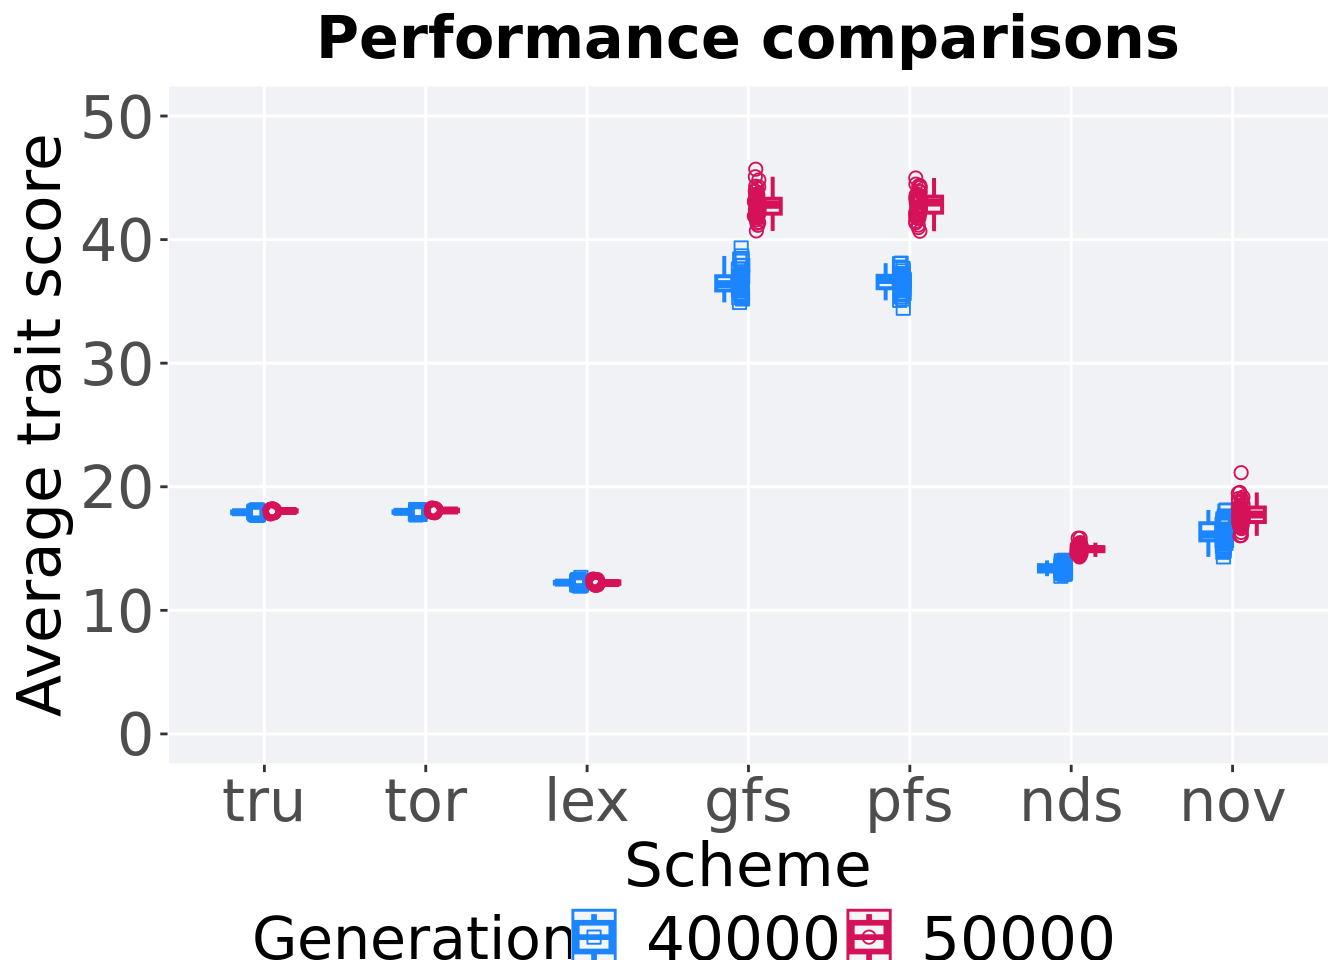
\includegraphics{demo_files/figure-latex/exp-mvc-per-sli-1.pdf}

\hypertarget{stats-3}{%
\subsubsection{Stats}\label{stats-3}}

Summary statistics for the performance of the best performance at 40,000 and 50,000 generations.

\begin{Shaded}
\begin{Highlighting}[]
\CommentTok{### performance comparisons and generation slices 40K & 50K}
\NormalTok{slices =}\StringTok{ }\KeywordTok{filter}\NormalTok{(cc_over_time_mvc, diagnostic }\OperatorTok{==}\StringTok{ 'exploitation_rate'} \OperatorTok{&}\StringTok{ }\NormalTok{(gen }\OperatorTok{==}\StringTok{ }\DecValTok{50000} \OperatorTok{|}\StringTok{ }\NormalTok{gen }\OperatorTok{==}\StringTok{ }\DecValTok{40000}\NormalTok{) }\OperatorTok{&}\StringTok{ }\NormalTok{acron }\OperatorTok{!=}\StringTok{ 'ran'}\NormalTok{)}
\NormalTok{slices}\OperatorTok{$}\NormalTok{Generation <-}\StringTok{ }\KeywordTok{factor}\NormalTok{(slices}\OperatorTok{$}\NormalTok{gen, }\DataTypeTok{levels =} \KeywordTok{c}\NormalTok{(}\DecValTok{50000}\NormalTok{,}\DecValTok{40000}\NormalTok{))}
\NormalTok{slices}\OperatorTok{$}\NormalTok{acron =}\StringTok{ }\KeywordTok{factor}\NormalTok{(slices}\OperatorTok{$}\NormalTok{acron, }\DataTypeTok{levels =} \KeywordTok{c}\NormalTok{(}\StringTok{'gfs'}\NormalTok{,}\StringTok{'pfs'}\NormalTok{,}\StringTok{'tru'}\NormalTok{,}\StringTok{'tor'}\NormalTok{,}\StringTok{'nov'}\NormalTok{, }\StringTok{'nds'}\NormalTok{,}\StringTok{'lex'}\NormalTok{, }\StringTok{'ran'}\NormalTok{))}
\NormalTok{slices }\OperatorTok
\StringTok{  }\KeywordTok{group_by}\NormalTok{(acron, Generation) }\OperatorTok
\StringTok{  }\NormalTok{dplyr}\OperatorTok{::}\KeywordTok{summarise}\NormalTok{(}
    \DataTypeTok{count =} \KeywordTok{n}\NormalTok{(),}
    \DataTypeTok{na_cnt =} \KeywordTok{sum}\NormalTok{(}\KeywordTok{is.na}\NormalTok{(pop_fit_max  }\OperatorTok{/}\StringTok{ }\NormalTok{DIMENSIONALITY)),}
    \DataTypeTok{min =} \KeywordTok{min}\NormalTok{(pop_fit_max  }\OperatorTok{/}\StringTok{ }\NormalTok{DIMENSIONALITY, }\DataTypeTok{na.rm =} \OtherTok{TRUE}\NormalTok{),}
    \DataTypeTok{median =} \KeywordTok{median}\NormalTok{(pop_fit_max  }\OperatorTok{/}\StringTok{ }\NormalTok{DIMENSIONALITY, }\DataTypeTok{na.rm =} \OtherTok{TRUE}\NormalTok{),}
    \DataTypeTok{mean =} \KeywordTok{mean}\NormalTok{(pop_fit_max  }\OperatorTok{/}\StringTok{ }\NormalTok{DIMENSIONALITY, }\DataTypeTok{na.rm =} \OtherTok{TRUE}\NormalTok{),}
    \DataTypeTok{max =} \KeywordTok{max}\NormalTok{(pop_fit_max  }\OperatorTok{/}\StringTok{ }\NormalTok{DIMENSIONALITY, }\DataTypeTok{na.rm =} \OtherTok{TRUE}\NormalTok{),}
    \DataTypeTok{IQR =} \KeywordTok{IQR}\NormalTok{(pop_fit_max  }\OperatorTok{/}\StringTok{ }\NormalTok{DIMENSIONALITY, }\DataTypeTok{na.rm =} \OtherTok{TRUE}\NormalTok{)}
\NormalTok{  )}
\end{Highlighting}
\end{Shaded}

\begin{verbatim}
## `summarise()` has grouped output by 'acron'. You can override using the
## `.groups` argument.
\end{verbatim}

\begin{verbatim}
## # A tibble: 14 x 9
## # Groups:   acron [7]
##    acron Generation count na_cnt   min median  mean   max   IQR
##    <fct> <fct>      <int>  <int> <dbl>  <dbl> <dbl> <dbl> <dbl>
##  1 gfs   50000         50      0  40.7   42.8  42.8  45.7 1.21 
##  2 gfs   40000         50      0  34.9   36.4  36.6  39.3 1.15 
##  3 pfs   50000         50      0  40.7   43.0  42.8  45.0 1.30 
##  4 pfs   40000         50      0  34.4   36.7  36.6  38.1 1.01 
##  5 tru   50000         50      0  17.8   18.0  18.0  18.2 0.118
##  6 tru   40000         50      0  17.7   17.9  17.9  18.1 0.147
##  7 tor   50000         50      0  17.9   18.1  18.1  18.3 0.130
##  8 tor   40000         50      0  17.7   18.0  18.0  18.2 0.115
##  9 nov   50000         50      0  16.0   17.8  17.8  21.1 1.17 
## 10 nov   40000         50      0  14.3   16.1  16.3  18.1 1.39 
## 11 nds   50000         50      0  14.3   15.0  15.0  15.8 0.327
## 12 nds   40000         50      0  12.8   13.4  13.4  14.0 0.516
## 13 lex   50000         50      0  12.0   12.2  12.2  12.5 0.199
## 14 lex   40000         50      0  12.0   12.2  12.2  12.7 0.132
\end{verbatim}

Truncation selection comparisons.

\begin{Shaded}
\begin{Highlighting}[]
\KeywordTok{wilcox.test}\NormalTok{(}\DataTypeTok{x =} \KeywordTok{filter}\NormalTok{(slices, acron }\OperatorTok{==}\StringTok{ 'tru'} \OperatorTok{&}\StringTok{ }\NormalTok{Generation }\OperatorTok{==}\StringTok{ }\DecValTok{50000}\NormalTok{)}\OperatorTok{$}\NormalTok{pop_fit_max,}
            \DataTypeTok{y =} \KeywordTok{filter}\NormalTok{(slices, acron }\OperatorTok{==}\StringTok{ 'tru'} \OperatorTok{&}\StringTok{ }\NormalTok{Generation }\OperatorTok{==}\StringTok{ }\DecValTok{40000}\NormalTok{)}\OperatorTok{$}\NormalTok{pop_fit_max,}
            \DataTypeTok{alternative =} \StringTok{'t'}\NormalTok{)}
\end{Highlighting}
\end{Shaded}

\begin{verbatim}
## 
##  Wilcoxon rank sum test with continuity correction
## 
## data:  filter(slices, acron == "tru" & Generation == 50000)$pop_fit_max and filter(slices, acron == "tru" & Generation == 40000)$pop_fit_max
## W = 2037.5, p-value = 5.705e-08
## alternative hypothesis: true location shift is not equal to 0
\end{verbatim}

Tournament selection comparisons.

\begin{Shaded}
\begin{Highlighting}[]
\KeywordTok{wilcox.test}\NormalTok{(}\DataTypeTok{x =} \KeywordTok{filter}\NormalTok{(slices, acron }\OperatorTok{==}\StringTok{ 'tor'} \OperatorTok{&}\StringTok{ }\NormalTok{Generation }\OperatorTok{==}\StringTok{ }\DecValTok{50000}\NormalTok{)}\OperatorTok{$}\NormalTok{pop_fit_max,}
            \DataTypeTok{y =} \KeywordTok{filter}\NormalTok{(slices, acron }\OperatorTok{==}\StringTok{ 'tor'} \OperatorTok{&}\StringTok{ }\NormalTok{Generation }\OperatorTok{==}\StringTok{ }\DecValTok{40000}\NormalTok{)}\OperatorTok{$}\NormalTok{pop_fit_max,}
            \DataTypeTok{alternative =} \StringTok{'t'}\NormalTok{)}
\end{Highlighting}
\end{Shaded}

\begin{verbatim}
## 
##  Wilcoxon rank sum test with continuity correction
## 
## data:  filter(slices, acron == "tor" & Generation == 50000)$pop_fit_max and filter(slices, acron == "tor" & Generation == 40000)$pop_fit_max
## W = 2075, p-value = 1.301e-08
## alternative hypothesis: true location shift is not equal to 0
\end{verbatim}

Lexicase selection comparisons.

\begin{Shaded}
\begin{Highlighting}[]
\KeywordTok{wilcox.test}\NormalTok{(}\DataTypeTok{x =} \KeywordTok{filter}\NormalTok{(slices, acron }\OperatorTok{==}\StringTok{ 'lex'} \OperatorTok{&}\StringTok{ }\NormalTok{Generation }\OperatorTok{==}\StringTok{ }\DecValTok{50000}\NormalTok{)}\OperatorTok{$}\NormalTok{pop_fit_max,}
            \DataTypeTok{y =} \KeywordTok{filter}\NormalTok{(slices, acron }\OperatorTok{==}\StringTok{ 'lex'} \OperatorTok{&}\StringTok{ }\NormalTok{Generation }\OperatorTok{==}\StringTok{ }\DecValTok{40000}\NormalTok{)}\OperatorTok{$}\NormalTok{pop_fit_max,}
            \DataTypeTok{alternative =} \StringTok{'t'}\NormalTok{)}
\end{Highlighting}
\end{Shaded}

\begin{verbatim}
## 
##  Wilcoxon rank sum test with continuity correction
## 
## data:  filter(slices, acron == "lex" & Generation == 50000)$pop_fit_max and filter(slices, acron == "lex" & Generation == 40000)$pop_fit_max
## W = 1260.5, p-value = 0.945
## alternative hypothesis: true location shift is not equal to 0
\end{verbatim}

Genotypic fitness sharing comparisons.

\begin{Shaded}
\begin{Highlighting}[]
\KeywordTok{wilcox.test}\NormalTok{(}\DataTypeTok{x =} \KeywordTok{filter}\NormalTok{(slices, acron }\OperatorTok{==}\StringTok{ 'gfs'} \OperatorTok{&}\StringTok{ }\NormalTok{Generation }\OperatorTok{==}\StringTok{ }\DecValTok{50000}\NormalTok{)}\OperatorTok{$}\NormalTok{pop_fit_max,}
            \DataTypeTok{y =} \KeywordTok{filter}\NormalTok{(slices, acron }\OperatorTok{==}\StringTok{ 'gfs'} \OperatorTok{&}\StringTok{ }\NormalTok{Generation }\OperatorTok{==}\StringTok{ }\DecValTok{40000}\NormalTok{)}\OperatorTok{$}\NormalTok{pop_fit_max,}
            \DataTypeTok{alternative =} \StringTok{'t'}\NormalTok{)}
\end{Highlighting}
\end{Shaded}

\begin{verbatim}
## 
##  Wilcoxon rank sum test with continuity correction
## 
## data:  filter(slices, acron == "gfs" & Generation == 50000)$pop_fit_max and filter(slices, acron == "gfs" & Generation == 40000)$pop_fit_max
## W = 2500, p-value < 2.2e-16
## alternative hypothesis: true location shift is not equal to 0
\end{verbatim}

Phenotypic fitness sharing comparisons.

\begin{Shaded}
\begin{Highlighting}[]
\KeywordTok{wilcox.test}\NormalTok{(}\DataTypeTok{x =} \KeywordTok{filter}\NormalTok{(slices, acron }\OperatorTok{==}\StringTok{ 'pfs'} \OperatorTok{&}\StringTok{ }\NormalTok{Generation }\OperatorTok{==}\StringTok{ }\DecValTok{50000}\NormalTok{)}\OperatorTok{$}\NormalTok{pop_fit_max,}
            \DataTypeTok{y =} \KeywordTok{filter}\NormalTok{(slices, acron }\OperatorTok{==}\StringTok{ 'pfs'} \OperatorTok{&}\StringTok{ }\NormalTok{Generation }\OperatorTok{==}\StringTok{ }\DecValTok{40000}\NormalTok{)}\OperatorTok{$}\NormalTok{pop_fit_max,}
            \DataTypeTok{alternative =} \StringTok{'t'}\NormalTok{)}
\end{Highlighting}
\end{Shaded}

\begin{verbatim}
## 
##  Wilcoxon rank sum test with continuity correction
## 
## data:  filter(slices, acron == "pfs" & Generation == 50000)$pop_fit_max and filter(slices, acron == "pfs" & Generation == 40000)$pop_fit_max
## W = 2500, p-value < 2.2e-16
## alternative hypothesis: true location shift is not equal to 0
\end{verbatim}

Nondominated sorting comparisons.

\begin{Shaded}
\begin{Highlighting}[]
\KeywordTok{wilcox.test}\NormalTok{(}\DataTypeTok{x =} \KeywordTok{filter}\NormalTok{(slices, acron }\OperatorTok{==}\StringTok{ 'nds'} \OperatorTok{&}\StringTok{ }\NormalTok{Generation }\OperatorTok{==}\StringTok{ }\DecValTok{50000}\NormalTok{)}\OperatorTok{$}\NormalTok{pop_fit_max,}
            \DataTypeTok{y =} \KeywordTok{filter}\NormalTok{(slices, acron }\OperatorTok{==}\StringTok{ 'nds'} \OperatorTok{&}\StringTok{ }\NormalTok{Generation }\OperatorTok{==}\StringTok{ }\DecValTok{40000}\NormalTok{)}\OperatorTok{$}\NormalTok{pop_fit_max,}
            \DataTypeTok{alternative =} \StringTok{'t'}\NormalTok{)}
\end{Highlighting}
\end{Shaded}

\begin{verbatim}
## 
##  Wilcoxon rank sum test with continuity correction
## 
## data:  filter(slices, acron == "nds" & Generation == 50000)$pop_fit_max and filter(slices, acron == "nds" & Generation == 40000)$pop_fit_max
## W = 2500, p-value < 2.2e-16
## alternative hypothesis: true location shift is not equal to 0
\end{verbatim}

Novelty search comparisons.

\begin{Shaded}
\begin{Highlighting}[]
\KeywordTok{wilcox.test}\NormalTok{(}\DataTypeTok{x =} \KeywordTok{filter}\NormalTok{(slices, acron }\OperatorTok{==}\StringTok{ 'nov'} \OperatorTok{&}\StringTok{ }\NormalTok{Generation }\OperatorTok{==}\StringTok{ }\DecValTok{50000}\NormalTok{)}\OperatorTok{$}\NormalTok{pop_fit_max,}
            \DataTypeTok{y =} \KeywordTok{filter}\NormalTok{(slices, acron }\OperatorTok{==}\StringTok{ 'nov'} \OperatorTok{&}\StringTok{ }\NormalTok{Generation }\OperatorTok{==}\StringTok{ }\DecValTok{40000}\NormalTok{)}\OperatorTok{$}\NormalTok{pop_fit_max,}
            \DataTypeTok{alternative =} \StringTok{'t'}\NormalTok{)}
\end{Highlighting}
\end{Shaded}

\begin{verbatim}
## 
##  Wilcoxon rank sum test with continuity correction
## 
## data:  filter(slices, acron == "nov" & Generation == 50000)$pop_fit_max and filter(slices, acron == "nov" & Generation == 40000)$pop_fit_max
## W = 2196, p-value = 7.119e-11
## alternative hypothesis: true location shift is not equal to 0
\end{verbatim}

\hypertarget{ordered-exploitation-results}{%
\chapter{Ordered exploitation results}\label{ordered-exploitation-results}}

Here we present the results for \textbf{best performances} found by each selection scheme replicate on the ordered exploitation diagnostic.
Best performance found refers to the largest average trait score found in a given population.
Note that performance values fall between 0.0 and 100.0.

\hypertarget{analysis-dependencies-1}{%
\section{Analysis dependencies}\label{analysis-dependencies-1}}

\begin{Shaded}
\begin{Highlighting}[]
\KeywordTok{library}\NormalTok{(ggplot2)}
\KeywordTok{library}\NormalTok{(cowplot)}
\KeywordTok{library}\NormalTok{(dplyr)}
\KeywordTok{library}\NormalTok{(PupillometryR)}
\KeywordTok{library}\NormalTok{(sdamr)}
\end{Highlighting}
\end{Shaded}

\hypertarget{performance-over-time-2}{%
\section{Performance over time}\label{performance-over-time-2}}

Best performance in a population over time.

\begin{Shaded}
\begin{Highlighting}[]
\CommentTok{# data for lines and shading on plots}
\NormalTok{lines =}\StringTok{ }\KeywordTok{filter}\NormalTok{(cc_over_time, diagnostic }\OperatorTok{==}\StringTok{ 'ordered_exploitation'}\NormalTok{) }\OperatorTok
\StringTok{  }\KeywordTok{group_by}\NormalTok{(}\StringTok{`}\DataTypeTok{Selection}\CharTok{\textbackslash{}n}\DataTypeTok{Scheme}\StringTok{`}\NormalTok{, gen) }\OperatorTok
\StringTok{  }\NormalTok{dplyr}\OperatorTok{::}\KeywordTok{summarise}\NormalTok{(}
    \DataTypeTok{min =} \KeywordTok{min}\NormalTok{(pop_fit_max) }\OperatorTok{/}\StringTok{ }\NormalTok{DIMENSIONALITY,}
    \DataTypeTok{mean =} \KeywordTok{mean}\NormalTok{(pop_fit_max) }\OperatorTok{/}\StringTok{ }\NormalTok{DIMENSIONALITY,}
    \DataTypeTok{max =} \KeywordTok{max}\NormalTok{(pop_fit_max) }\OperatorTok{/}\StringTok{ }\NormalTok{DIMENSIONALITY}
\NormalTok{  )}
\end{Highlighting}
\end{Shaded}

\begin{verbatim}
## `summarise()` has grouped output by 'Selection Scheme'. You can override using
## the `.groups` argument.
\end{verbatim}

\begin{Shaded}
\begin{Highlighting}[]
\KeywordTok{ggplot}\NormalTok{(lines, }\KeywordTok{aes}\NormalTok{(}\DataTypeTok{x=}\NormalTok{gen, }\DataTypeTok{y=}\NormalTok{mean, }\DataTypeTok{group =} \StringTok{`}\DataTypeTok{Selection}\CharTok{\textbackslash{}n}\DataTypeTok{Scheme}\StringTok{`}\NormalTok{, }\DataTypeTok{fill =}\StringTok{`}\DataTypeTok{Selection}\CharTok{\textbackslash{}n}\DataTypeTok{Scheme}\StringTok{`}\NormalTok{, }\DataTypeTok{color =} \StringTok{`}\DataTypeTok{Selection}\CharTok{\textbackslash{}n}\DataTypeTok{Scheme}\StringTok{`}\NormalTok{, }\DataTypeTok{shape =} \StringTok{`}\DataTypeTok{Selection}\CharTok{\textbackslash{}n}\DataTypeTok{Scheme}\StringTok{`}\NormalTok{)) }\OperatorTok{+}
\StringTok{  }\KeywordTok{geom_ribbon}\NormalTok{(}\KeywordTok{aes}\NormalTok{(}\DataTypeTok{ymin =}\NormalTok{ min, }\DataTypeTok{ymax =}\NormalTok{ max), }\DataTypeTok{alpha =} \FloatTok{0.1}\NormalTok{) }\OperatorTok{+}
\StringTok{  }\KeywordTok{geom_line}\NormalTok{(}\DataTypeTok{size =} \FloatTok{0.5}\NormalTok{) }\OperatorTok{+}
\StringTok{  }\KeywordTok{geom_point}\NormalTok{(}\DataTypeTok{data =} \KeywordTok{filter}\NormalTok{(lines, gen }\OperatorTok\StringTok{ }\DecValTok{2000} \OperatorTok{==}\StringTok{ }\DecValTok{0} \OperatorTok{&}\StringTok{ }\NormalTok{gen }\OperatorTok{!=}\StringTok{ }\DecValTok{0}\NormalTok{), }\DataTypeTok{size =} \FloatTok{1.5}\NormalTok{, }\DataTypeTok{stroke =} \FloatTok{2.0}\NormalTok{, }\DataTypeTok{alpha =} \FloatTok{1.0}\NormalTok{) }\OperatorTok{+}
\StringTok{  }\KeywordTok{scale_y_continuous}\NormalTok{(}
    \DataTypeTok{name=}\StringTok{"Average trait score"}\NormalTok{,}
    \DataTypeTok{limits=}\KeywordTok{c}\NormalTok{(}\DecValTok{0}\NormalTok{, }\DecValTok{100}\NormalTok{),}
    \DataTypeTok{breaks=}\KeywordTok{seq}\NormalTok{(}\DecValTok{0}\NormalTok{,}\DecValTok{100}\NormalTok{, }\DecValTok{20}\NormalTok{),}
    \DataTypeTok{labels=}\KeywordTok{c}\NormalTok{(}\StringTok{"0"}\NormalTok{, }\StringTok{"20"}\NormalTok{, }\StringTok{"40"}\NormalTok{, }\StringTok{"60"}\NormalTok{, }\StringTok{"80"}\NormalTok{, }\StringTok{"100"}\NormalTok{)}
\NormalTok{  ) }\OperatorTok{+}
\StringTok{  }\KeywordTok{scale_x_continuous}\NormalTok{(}
    \DataTypeTok{name=}\StringTok{"Generations"}\NormalTok{,}
    \DataTypeTok{limits=}\KeywordTok{c}\NormalTok{(}\DecValTok{0}\NormalTok{, }\DecValTok{50000}\NormalTok{),}
    \DataTypeTok{breaks=}\KeywordTok{c}\NormalTok{(}\DecValTok{0}\NormalTok{, }\DecValTok{10000}\NormalTok{, }\DecValTok{20000}\NormalTok{, }\DecValTok{30000}\NormalTok{, }\DecValTok{40000}\NormalTok{, }\DecValTok{50000}\NormalTok{),}
    \DataTypeTok{labels=}\KeywordTok{c}\NormalTok{(}\StringTok{"0e+4"}\NormalTok{, }\StringTok{"1e+4"}\NormalTok{, }\StringTok{"2e+4"}\NormalTok{, }\StringTok{"3e+4"}\NormalTok{, }\StringTok{"4e+4"}\NormalTok{, }\StringTok{"5e+4"}\NormalTok{)}

\NormalTok{  ) }\OperatorTok{+}
\StringTok{  }\KeywordTok{scale_shape_manual}\NormalTok{(}\DataTypeTok{values=}\NormalTok{SHAPE)}\OperatorTok{+}
\StringTok{  }\KeywordTok{scale_colour_manual}\NormalTok{(}\DataTypeTok{values =}\NormalTok{ cb_palette) }\OperatorTok{+}
\StringTok{  }\KeywordTok{scale_fill_manual}\NormalTok{(}\DataTypeTok{values =}\NormalTok{ cb_palette) }\OperatorTok{+}
\StringTok{  }\KeywordTok{ggtitle}\NormalTok{(}\StringTok{'Performance over time'}\NormalTok{)}\OperatorTok{+}
\StringTok{  }\NormalTok{p_theme }\OperatorTok{+}\StringTok{ }\KeywordTok{theme}\NormalTok{(}\DataTypeTok{legend.title=}\KeywordTok{element_blank}\NormalTok{(),}\DataTypeTok{legend.text=}\KeywordTok{element_text}\NormalTok{(}\DataTypeTok{size=}\DecValTok{11}\NormalTok{)) }\OperatorTok{+}
\StringTok{  }\KeywordTok{guides}\NormalTok{(}
    \DataTypeTok{shape=}\KeywordTok{guide_legend}\NormalTok{(}\DataTypeTok{ncol=}\DecValTok{2}\NormalTok{, }\DataTypeTok{title.position =} \StringTok{"bottom"}\NormalTok{),}
    \DataTypeTok{color=}\KeywordTok{guide_legend}\NormalTok{(}\DataTypeTok{ncol=}\DecValTok{2}\NormalTok{, }\DataTypeTok{title.position =} \StringTok{"bottom"}\NormalTok{),}
    \DataTypeTok{fill=}\KeywordTok{guide_legend}\NormalTok{(}\DataTypeTok{ncol=}\DecValTok{2}\NormalTok{, }\DataTypeTok{title.position =} \StringTok{"bottom"}\NormalTok{)}
\NormalTok{  )}
\end{Highlighting}
\end{Shaded}

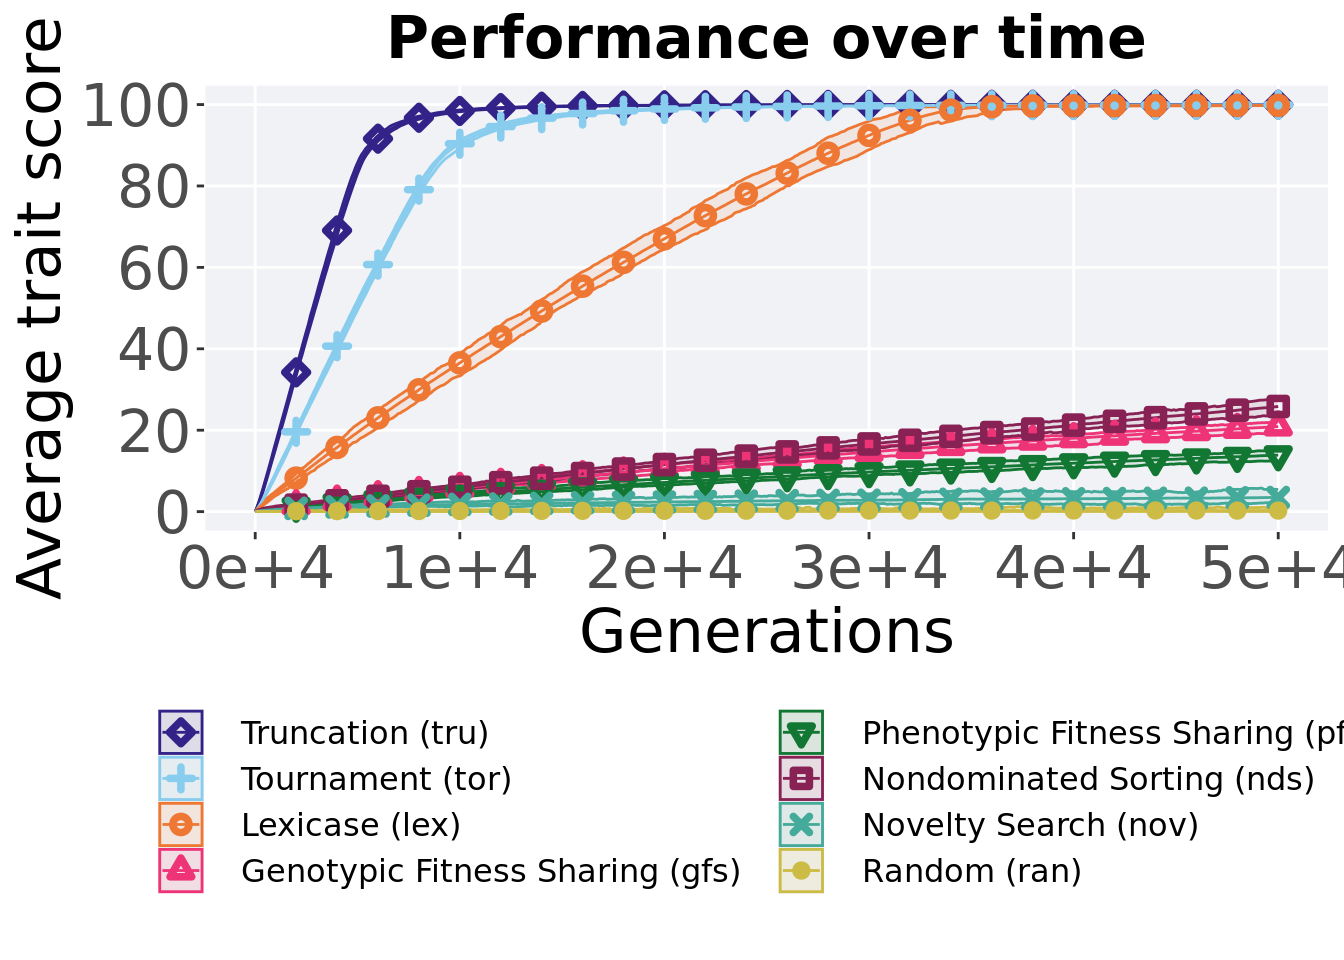
\includegraphics{demo_files/figure-latex/ord-per-ot-1.pdf}

\hypertarget{best-performance-throughout-2}{%
\section{Best performance throughout}\label{best-performance-throughout-2}}

Best performance found throughout 50,000 generations.

\begin{Shaded}
\begin{Highlighting}[]
\CommentTok{### best performance throughout}
\KeywordTok{filter}\NormalTok{(cc_best, col }\OperatorTok{==}\StringTok{ 'pop_fit_max'} \OperatorTok{&}\StringTok{ }\NormalTok{diagnostic }\OperatorTok{==}\StringTok{ 'ordered_exploitation'}\NormalTok{) }\OperatorTok
\StringTok{  }\KeywordTok{ggplot}\NormalTok{(., }\KeywordTok{aes}\NormalTok{(}\DataTypeTok{x =}\NormalTok{ acron, }\DataTypeTok{y =}\NormalTok{ val }\OperatorTok{/}\StringTok{ }\NormalTok{DIMENSIONALITY, }\DataTypeTok{color =}\NormalTok{ acron, }\DataTypeTok{fill =}\NormalTok{ acron, }\DataTypeTok{shape =}\NormalTok{ acron)) }\OperatorTok{+}
\StringTok{  }\KeywordTok{geom_flat_violin}\NormalTok{(}\DataTypeTok{position =} \KeywordTok{position_nudge}\NormalTok{(}\DataTypeTok{x =} \FloatTok{.2}\NormalTok{, }\DataTypeTok{y =} \DecValTok{0}\NormalTok{), }\DataTypeTok{scale =} \StringTok{'width'}\NormalTok{, }\DataTypeTok{alpha =} \FloatTok{0.2}\NormalTok{) }\OperatorTok{+}
\StringTok{  }\KeywordTok{geom_point}\NormalTok{(}\DataTypeTok{position =} \KeywordTok{position_jitter}\NormalTok{(}\DataTypeTok{width =} \FloatTok{.1}\NormalTok{), }\DataTypeTok{size =} \FloatTok{1.5}\NormalTok{, }\DataTypeTok{alpha =} \FloatTok{1.0}\NormalTok{) }\OperatorTok{+}
\StringTok{  }\KeywordTok{geom_boxplot}\NormalTok{(}\DataTypeTok{color =} \StringTok{'black'}\NormalTok{, }\DataTypeTok{width =} \FloatTok{.2}\NormalTok{, }\DataTypeTok{outlier.shape =} \OtherTok{NA}\NormalTok{, }\DataTypeTok{alpha =} \FloatTok{0.0}\NormalTok{) }\OperatorTok{+}
\StringTok{  }\KeywordTok{scale_y_continuous}\NormalTok{(}
    \DataTypeTok{name=}\StringTok{"Average trait score"}\NormalTok{,}
    \DataTypeTok{limits=}\KeywordTok{c}\NormalTok{(}\OperatorTok{-}\DecValTok{1}\NormalTok{, }\DecValTok{101}\NormalTok{),}
    \DataTypeTok{breaks=}\KeywordTok{seq}\NormalTok{(}\DecValTok{0}\NormalTok{,}\DecValTok{100}\NormalTok{, }\DecValTok{20}\NormalTok{),}
    \DataTypeTok{labels=}\KeywordTok{c}\NormalTok{(}\StringTok{"0"}\NormalTok{, }\StringTok{"20"}\NormalTok{, }\StringTok{"40"}\NormalTok{, }\StringTok{"60"}\NormalTok{, }\StringTok{"80"}\NormalTok{, }\StringTok{"100"}\NormalTok{)}
\NormalTok{  ) }\OperatorTok{+}
\StringTok{  }\KeywordTok{scale_x_discrete}\NormalTok{(}
    \DataTypeTok{name=}\StringTok{"Scheme"}
\NormalTok{  )}\OperatorTok{+}
\StringTok{  }\KeywordTok{scale_shape_manual}\NormalTok{(}\DataTypeTok{values=}\NormalTok{SHAPE)}\OperatorTok{+}
\StringTok{  }\KeywordTok{scale_colour_manual}\NormalTok{(}\DataTypeTok{values =}\NormalTok{ cb_palette, ) }\OperatorTok{+}
\StringTok{  }\KeywordTok{scale_fill_manual}\NormalTok{(}\DataTypeTok{values =}\NormalTok{ cb_palette) }\OperatorTok{+}
\StringTok{  }\KeywordTok{ggtitle}\NormalTok{(}\StringTok{'Best performance throughout'}\NormalTok{)}\OperatorTok{+}
\StringTok{  }\NormalTok{p_theme }\OperatorTok{+}\StringTok{ }\KeywordTok{theme}\NormalTok{(}\DataTypeTok{legend.title=}\KeywordTok{element_blank}\NormalTok{()) }\OperatorTok{+}
\StringTok{  }\KeywordTok{guides}\NormalTok{(}
    \DataTypeTok{shape=}\KeywordTok{guide_legend}\NormalTok{(}\DataTypeTok{nrow=}\DecValTok{2}\NormalTok{, }\DataTypeTok{title.position =} \StringTok{"bottom"}\NormalTok{),}
    \DataTypeTok{color=}\KeywordTok{guide_legend}\NormalTok{(}\DataTypeTok{nrow=}\DecValTok{2}\NormalTok{, }\DataTypeTok{title.position =} \StringTok{"bottom"}\NormalTok{),}
    \DataTypeTok{fill=}\KeywordTok{guide_legend}\NormalTok{(}\DataTypeTok{nrow=}\DecValTok{2}\NormalTok{, }\DataTypeTok{title.position =} \StringTok{"bottom"}\NormalTok{)}
\NormalTok{  )}
\end{Highlighting}
\end{Shaded}

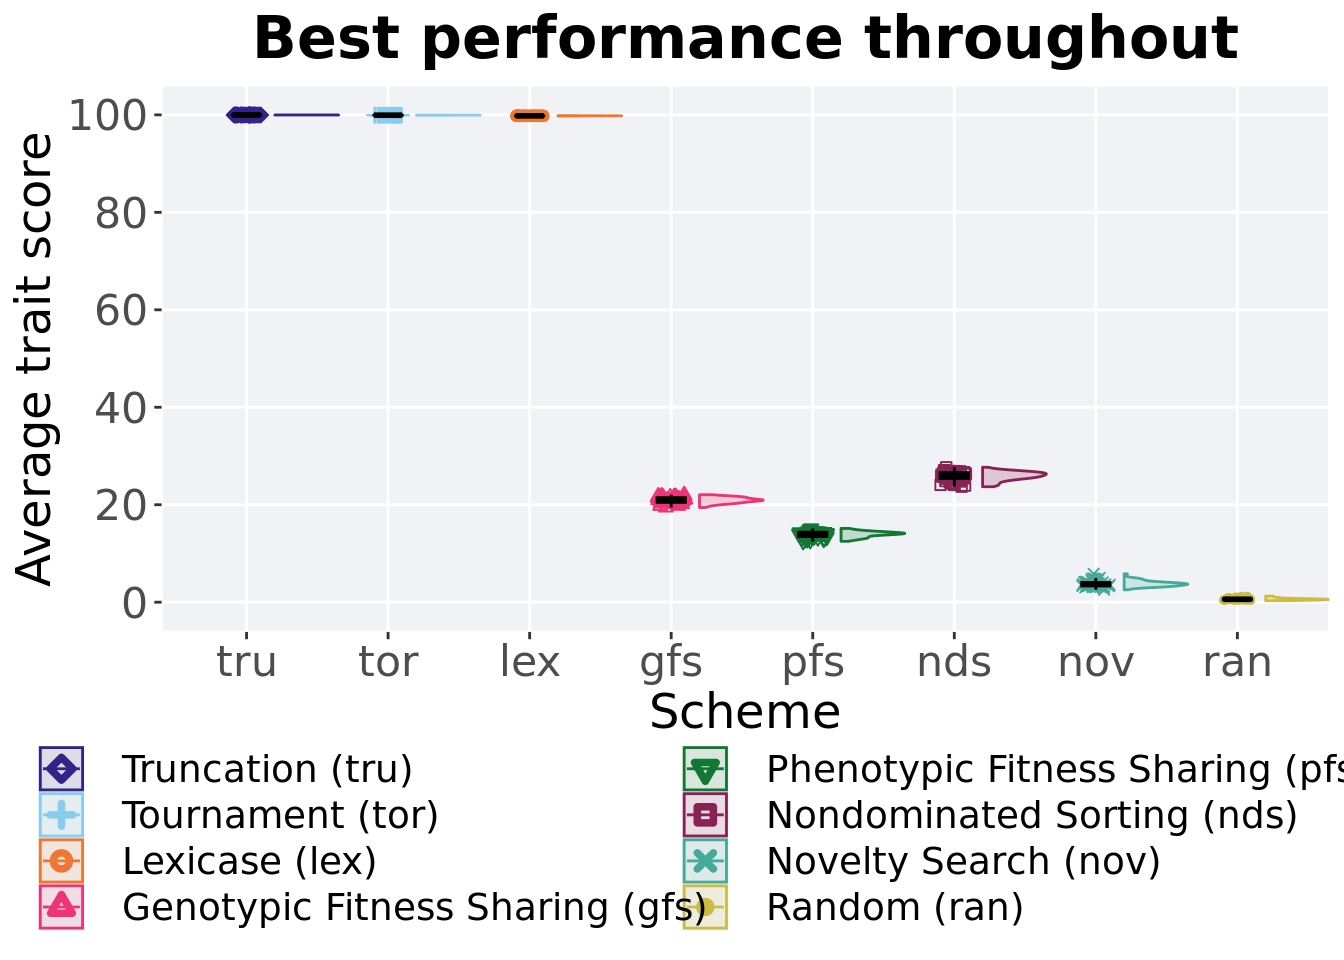
\includegraphics{demo_files/figure-latex/ord-per-bst-1.pdf}

\hypertarget{stats-4}{%
\subsection{Stats}\label{stats-4}}

Summary statistics for the performance of the best performance throughout 50,000 generations.

\begin{Shaded}
\begin{Highlighting}[]
\CommentTok{#get data & summarize}
\NormalTok{performance =}\StringTok{ }\KeywordTok{filter}\NormalTok{(cc_best, col }\OperatorTok{==}\StringTok{ 'pop_fit_max'} \OperatorTok{&}\StringTok{ }\NormalTok{diagnostic }\OperatorTok{==}\StringTok{ 'ordered_exploitation'}\NormalTok{)}
\NormalTok{performance}\OperatorTok{$}\NormalTok{acron =}\StringTok{ }\KeywordTok{factor}\NormalTok{(performance}\OperatorTok{$}\NormalTok{acron, }\DataTypeTok{levels =} \KeywordTok{c}\NormalTok{(}\StringTok{'tru'}\NormalTok{, }\StringTok{'tor'}\NormalTok{, }\StringTok{'lex'}\NormalTok{,}\StringTok{'nds'}\NormalTok{, }\StringTok{'gfs'}\NormalTok{, }\StringTok{'pfs'}\NormalTok{, }\StringTok{'nov'}\NormalTok{,  }\StringTok{'ran'}\NormalTok{))}
\NormalTok{performance }\OperatorTok
\StringTok{  }\KeywordTok{group_by}\NormalTok{(acron) }\OperatorTok
\StringTok{  }\NormalTok{dplyr}\OperatorTok{::}\KeywordTok{summarise}\NormalTok{(}
    \DataTypeTok{count =} \KeywordTok{n}\NormalTok{(),}
    \DataTypeTok{na_cnt =} \KeywordTok{sum}\NormalTok{(}\KeywordTok{is.na}\NormalTok{(val)),}
    \DataTypeTok{min =} \KeywordTok{min}\NormalTok{(val }\OperatorTok{/}\StringTok{ }\NormalTok{DIMENSIONALITY, }\DataTypeTok{na.rm =} \OtherTok{TRUE}\NormalTok{),}
    \DataTypeTok{median =} \KeywordTok{median}\NormalTok{(val }\OperatorTok{/}\StringTok{ }\NormalTok{DIMENSIONALITY, }\DataTypeTok{na.rm =} \OtherTok{TRUE}\NormalTok{),}
    \DataTypeTok{mean =} \KeywordTok{mean}\NormalTok{(val }\OperatorTok{/}\StringTok{ }\NormalTok{DIMENSIONALITY, }\DataTypeTok{na.rm =} \OtherTok{TRUE}\NormalTok{),}
    \DataTypeTok{max =} \KeywordTok{max}\NormalTok{(val }\OperatorTok{/}\StringTok{ }\NormalTok{DIMENSIONALITY, }\DataTypeTok{na.rm =} \OtherTok{TRUE}\NormalTok{),}
    \DataTypeTok{IQR =} \KeywordTok{IQR}\NormalTok{(val }\OperatorTok{/}\StringTok{ }\NormalTok{DIMENSIONALITY, }\DataTypeTok{na.rm =} \OtherTok{TRUE}\NormalTok{)}
\NormalTok{  )}
\end{Highlighting}
\end{Shaded}

\begin{verbatim}
## # A tibble: 8 x 8
##   acron count na_cnt     min  median    mean    max     IQR
##   <fct> <int>  <int>   <dbl>   <dbl>   <dbl>  <dbl>   <dbl>
## 1 tru      50      0 100.    100.    100.    100.   0.00208
## 2 tor      50      0  99.9    99.9    99.9    99.9  0.00445
## 3 lex      50      0  99.8    99.8    99.8    99.8  0.0207 
## 4 nds      50      0  23.7    26.0    25.9    27.7  1.17   
## 5 gfs      50      0  19.4    21.0    20.9    22.1  0.970  
## 6 pfs      50      0  12.5    14.1    13.9    15.1  0.871  
## 7 nov      50      0   2.55    3.70    3.80    5.82 0.718  
## 8 ran      50      0   0.319   0.598   0.634   1.26 0.240
\end{verbatim}

Kruskal--Wallis test provides evidence of statistical differences.

\begin{Shaded}
\begin{Highlighting}[]
\KeywordTok{kruskal.test}\NormalTok{(val }\OperatorTok{~}\StringTok{ }\NormalTok{acron, }\DataTypeTok{data =}\NormalTok{ performance)}
\end{Highlighting}
\end{Shaded}

\begin{verbatim}
## 
##  Kruskal-Wallis rank sum test
## 
## data:  val by acron
## Kruskal-Wallis chi-squared = 392.77, df = 7, p-value < 2.2e-16
\end{verbatim}

Results for post-hoc Wilcoxon rank-sum test with a Bonferroni correction.

\begin{Shaded}
\begin{Highlighting}[]
\KeywordTok{pairwise.wilcox.test}\NormalTok{(}\DataTypeTok{x =}\NormalTok{ performance}\OperatorTok{$}\NormalTok{val, }\DataTypeTok{g =}\NormalTok{ performance}\OperatorTok{$}\NormalTok{acron, }\DataTypeTok{p.adjust.method =} \StringTok{"bonferroni"}\NormalTok{,}
                     \DataTypeTok{paired =} \OtherTok{FALSE}\NormalTok{, }\DataTypeTok{conf.int =} \OtherTok{FALSE}\NormalTok{, }\DataTypeTok{alternative =} \StringTok{'l'}\NormalTok{)}
\end{Highlighting}
\end{Shaded}

\begin{verbatim}
## 
##  Pairwise comparisons using Wilcoxon rank sum test with continuity correction 
## 
## data:  performance$val and performance$acron 
## 
##     tru    tor    lex    nds    gfs    pfs    nov   
## tor <2e-16 -      -      -      -      -      -     
## lex <2e-16 <2e-16 -      -      -      -      -     
## nds <2e-16 <2e-16 <2e-16 -      -      -      -     
## gfs <2e-16 <2e-16 <2e-16 <2e-16 -      -      -     
## pfs <2e-16 <2e-16 <2e-16 <2e-16 <2e-16 -      -     
## nov <2e-16 <2e-16 <2e-16 <2e-16 <2e-16 <2e-16 -     
## ran <2e-16 <2e-16 <2e-16 <2e-16 <2e-16 <2e-16 <2e-16
## 
## P value adjustment method: bonferroni
\end{verbatim}

\hypertarget{generation-satisfactory-solution-found-1}{%
\section{Generation satisfactory solution found}\label{generation-satisfactory-solution-found-1}}

First generation a satisfactory solution is found throughout the 50,000 generations.

\begin{Shaded}
\begin{Highlighting}[]
\CommentTok{### satisfactory solution found}
\KeywordTok{filter}\NormalTok{(cc_ssf, diagnostic }\OperatorTok{==}\StringTok{ 'ordered_exploitation'}\NormalTok{) }\OperatorTok
\StringTok{  }\KeywordTok{ggplot}\NormalTok{(., }\KeywordTok{aes}\NormalTok{(}\DataTypeTok{x =}\NormalTok{ acron, }\DataTypeTok{y =}\NormalTok{ Generations , }\DataTypeTok{color =}\NormalTok{ acron, }\DataTypeTok{fill =}\NormalTok{ acron, }\DataTypeTok{shape =}\NormalTok{ acron)) }\OperatorTok{+}
\StringTok{  }\KeywordTok{geom_flat_violin}\NormalTok{(}\DataTypeTok{position =} \KeywordTok{position_nudge}\NormalTok{(}\DataTypeTok{x =} \FloatTok{.2}\NormalTok{, }\DataTypeTok{y =} \DecValTok{0}\NormalTok{), }\DataTypeTok{scale =} \StringTok{'width'}\NormalTok{, }\DataTypeTok{alpha =} \FloatTok{0.2}\NormalTok{) }\OperatorTok{+}
\StringTok{  }\KeywordTok{geom_point}\NormalTok{(}\DataTypeTok{position =} \KeywordTok{position_jitter}\NormalTok{(}\DataTypeTok{width =} \FloatTok{.1}\NormalTok{), }\DataTypeTok{size =} \FloatTok{1.5}\NormalTok{, }\DataTypeTok{alpha =} \FloatTok{1.0}\NormalTok{) }\OperatorTok{+}
\StringTok{  }\KeywordTok{geom_boxplot}\NormalTok{(}\DataTypeTok{color =} \StringTok{'black'}\NormalTok{, }\DataTypeTok{width =} \FloatTok{.2}\NormalTok{, }\DataTypeTok{outlier.shape =} \OtherTok{NA}\NormalTok{, }\DataTypeTok{alpha =} \FloatTok{0.0}\NormalTok{) }\OperatorTok{+}
\StringTok{  }\KeywordTok{scale_y_continuous}\NormalTok{(}
    \DataTypeTok{name=}\StringTok{"Generation"}\NormalTok{,}
    \DataTypeTok{limits=}\KeywordTok{c}\NormalTok{(}\DecValTok{0}\NormalTok{, }\DecValTok{60001}\NormalTok{),}
    \DataTypeTok{breaks=}\KeywordTok{c}\NormalTok{(}\DecValTok{0}\NormalTok{, }\DecValTok{10000}\NormalTok{, }\DecValTok{20000}\NormalTok{, }\DecValTok{30000}\NormalTok{, }\DecValTok{40000}\NormalTok{, }\DecValTok{50000}\NormalTok{, }\DecValTok{60000}\NormalTok{),}
    \DataTypeTok{labels=}\KeywordTok{c}\NormalTok{(}\StringTok{"0e+4"}\NormalTok{, }\StringTok{"1e+4"}\NormalTok{, }\StringTok{"2e+4"}\NormalTok{, }\StringTok{"3e+4"}\NormalTok{, }\StringTok{"4e+4"}\NormalTok{, }\StringTok{"5e+4"}\NormalTok{, }\StringTok{"Fail"}\NormalTok{)}
\NormalTok{  ) }\OperatorTok{+}
\StringTok{  }\KeywordTok{scale_x_discrete}\NormalTok{(}
    \DataTypeTok{name=}\StringTok{"Scheme"}
\NormalTok{  )}\OperatorTok{+}
\StringTok{  }\KeywordTok{scale_shape_manual}\NormalTok{(}\DataTypeTok{values=}\NormalTok{SHAPE)}\OperatorTok{+}
\StringTok{  }\KeywordTok{scale_colour_manual}\NormalTok{(}\DataTypeTok{values =}\NormalTok{ cb_palette, ) }\OperatorTok{+}
\StringTok{  }\KeywordTok{scale_fill_manual}\NormalTok{(}\DataTypeTok{values =}\NormalTok{ cb_palette) }\OperatorTok{+}
\StringTok{  }\KeywordTok{ggtitle}\NormalTok{(}\StringTok{'Generation satisfactory solution found'}\NormalTok{)}\OperatorTok{+}
\StringTok{  }\NormalTok{p_theme }\OperatorTok{+}\StringTok{ }\KeywordTok{theme}\NormalTok{(}\DataTypeTok{legend.title=}\KeywordTok{element_blank}\NormalTok{()) }\OperatorTok{+}
\StringTok{  }\KeywordTok{guides}\NormalTok{(}
    \DataTypeTok{shape=}\KeywordTok{guide_legend}\NormalTok{(}\DataTypeTok{nrow=}\DecValTok{2}\NormalTok{, }\DataTypeTok{title.position =} \StringTok{"bottom"}\NormalTok{),}
    \DataTypeTok{color=}\KeywordTok{guide_legend}\NormalTok{(}\DataTypeTok{nrow=}\DecValTok{2}\NormalTok{, }\DataTypeTok{title.position =} \StringTok{"bottom"}\NormalTok{),}
    \DataTypeTok{fill=}\KeywordTok{guide_legend}\NormalTok{(}\DataTypeTok{nrow=}\DecValTok{2}\NormalTok{, }\DataTypeTok{title.position =} \StringTok{"bottom"}\NormalTok{)}
\NormalTok{  )}
\end{Highlighting}
\end{Shaded}

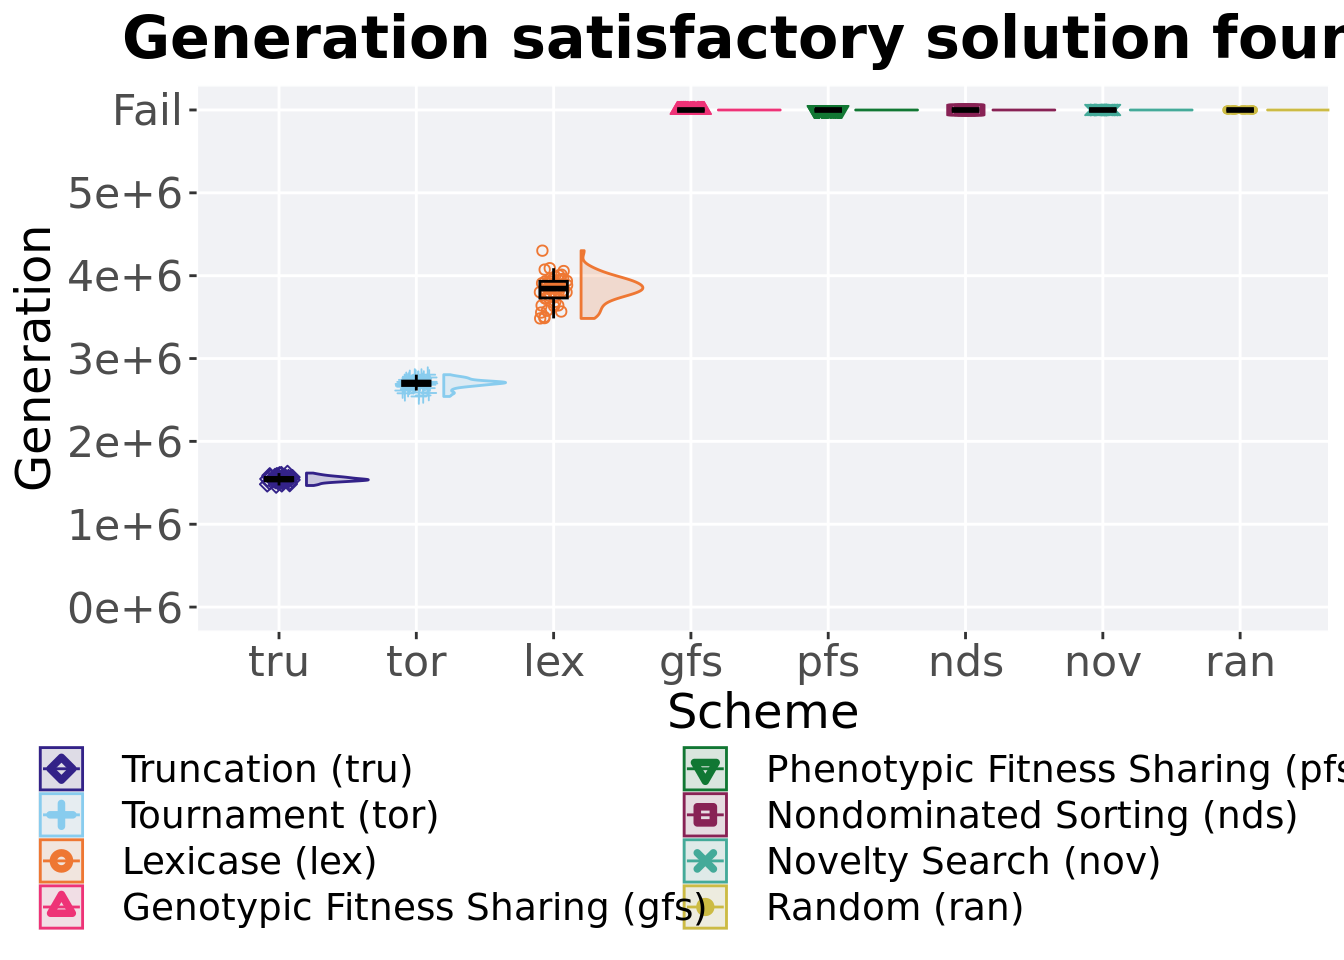
\includegraphics{demo_files/figure-latex/ord-ssf-1.pdf}

\hypertarget{stats-5}{%
\subsection{Stats}\label{stats-5}}

Summary statistics for the first generation a satisfactory solution is found throughout the 50,000 generations.

\begin{Shaded}
\begin{Highlighting}[]
\CommentTok{### Generation satisfactory solution found}
\NormalTok{ssf =}\StringTok{ }\KeywordTok{filter}\NormalTok{(cc_ssf, diagnostic }\OperatorTok{==}\StringTok{ 'ordered_exploitation'}  \OperatorTok{&}\StringTok{ }\NormalTok{Generations }\OperatorTok{<}\StringTok{ }\DecValTok{60000}\NormalTok{)}
\NormalTok{ssf}\OperatorTok{$}\NormalTok{acron =}\StringTok{ }\KeywordTok{factor}\NormalTok{(ssf}\OperatorTok{$}\NormalTok{acron, }\DataTypeTok{levels =} \KeywordTok{c}\NormalTok{(}\StringTok{'tru'}\NormalTok{, }\StringTok{'tor'}\NormalTok{, }\StringTok{'lex'}\NormalTok{))}
\NormalTok{ssf }\OperatorTok
\StringTok{  }\KeywordTok{group_by}\NormalTok{(acron) }\OperatorTok
\StringTok{  }\NormalTok{dplyr}\OperatorTok{::}\KeywordTok{summarise}\NormalTok{(}
    \DataTypeTok{count =} \KeywordTok{n}\NormalTok{(),}
    \DataTypeTok{na_cnt =} \KeywordTok{sum}\NormalTok{(}\KeywordTok{is.na}\NormalTok{(Generations)),}
    \DataTypeTok{min =} \KeywordTok{min}\NormalTok{(Generations, }\DataTypeTok{na.rm =} \OtherTok{TRUE}\NormalTok{),}
    \DataTypeTok{median =} \KeywordTok{median}\NormalTok{(Generations, }\DataTypeTok{na.rm =} \OtherTok{TRUE}\NormalTok{),}
    \DataTypeTok{mean =} \KeywordTok{mean}\NormalTok{(Generations, }\DataTypeTok{na.rm =} \OtherTok{TRUE}\NormalTok{),}
    \DataTypeTok{max =} \KeywordTok{max}\NormalTok{(Generations, }\DataTypeTok{na.rm =} \OtherTok{TRUE}\NormalTok{),}
    \DataTypeTok{IQR =} \KeywordTok{IQR}\NormalTok{(Generations, }\DataTypeTok{na.rm =} \OtherTok{TRUE}\NormalTok{)}
\NormalTok{  )}
\end{Highlighting}
\end{Shaded}

\begin{verbatim}
## # A tibble: 3 x 8
##   acron count na_cnt   min median   mean   max   IQR
##   <fct> <int>  <int> <int>  <dbl>  <dbl> <int> <dbl>
## 1 tru      50      0 14701 15466. 15511. 16280  422.
## 2 tor      50      0 25563 27254. 27122. 28151  714 
## 3 lex      50      0 35240 38918. 38865. 43751 2316.
\end{verbatim}

Kruskal--Wallis test provides evidence of difference amoung selection schemes.

\begin{Shaded}
\begin{Highlighting}[]
\KeywordTok{kruskal.test}\NormalTok{(Generations }\OperatorTok{~}\StringTok{ }\NormalTok{acron, }\DataTypeTok{data =}\NormalTok{ ssf)}
\end{Highlighting}
\end{Shaded}

\begin{verbatim}
## 
##  Kruskal-Wallis rank sum test
## 
## data:  Generations by acron
## Kruskal-Wallis chi-squared = 132.45, df = 2, p-value < 2.2e-16
\end{verbatim}

Results for post-hoc Wilcoxon rank-sum test with a Bonferroni correction.

\begin{Shaded}
\begin{Highlighting}[]
\KeywordTok{pairwise.wilcox.test}\NormalTok{(}\DataTypeTok{x =}\NormalTok{ ssf}\OperatorTok{$}\NormalTok{Generations, }\DataTypeTok{g =}\NormalTok{ ssf}\OperatorTok{$}\NormalTok{acron, }\DataTypeTok{p.adjust.method =} \StringTok{"bonferroni"}\NormalTok{,}
                     \DataTypeTok{paired =} \OtherTok{FALSE}\NormalTok{, }\DataTypeTok{conf.int =} \OtherTok{FALSE}\NormalTok{, }\DataTypeTok{alternative =} \StringTok{'g'}\NormalTok{)}
\end{Highlighting}
\end{Shaded}

\begin{verbatim}
## 
##  Pairwise comparisons using Wilcoxon rank sum test with continuity correction 
## 
## data:  ssf$Generations and ssf$acron 
## 
##     tru    tor   
## tor <2e-16 -     
## lex <2e-16 <2e-16
## 
## P value adjustment method: bonferroni
\end{verbatim}

\hypertarget{multi-valley-crossing-results-1}{%
\section{Multi-valley crossing results}\label{multi-valley-crossing-results-1}}

\hypertarget{performance-over-time-3}{%
\subsection{Performance over time}\label{performance-over-time-3}}

Best performance in a population over time.

\begin{Shaded}
\begin{Highlighting}[]
\CommentTok{# data for lines and shading on plots}
\NormalTok{lines =}\StringTok{ }\KeywordTok{filter}\NormalTok{(cc_over_time_mvc, diagnostic }\OperatorTok{==}\StringTok{ 'ordered_exploitation'}\NormalTok{) }\OperatorTok
\StringTok{  }\KeywordTok{group_by}\NormalTok{(}\StringTok{`}\DataTypeTok{Selection}\CharTok{\textbackslash{}n}\DataTypeTok{Scheme}\StringTok{`}\NormalTok{, gen) }\OperatorTok
\StringTok{  }\NormalTok{dplyr}\OperatorTok{::}\KeywordTok{summarise}\NormalTok{(}
    \DataTypeTok{min =} \KeywordTok{min}\NormalTok{(pop_fit_max) }\OperatorTok{/}\StringTok{ }\NormalTok{DIMENSIONALITY,}
    \DataTypeTok{mean =} \KeywordTok{mean}\NormalTok{(pop_fit_max) }\OperatorTok{/}\StringTok{ }\NormalTok{DIMENSIONALITY,}
    \DataTypeTok{max =} \KeywordTok{max}\NormalTok{(pop_fit_max) }\OperatorTok{/}\StringTok{ }\NormalTok{DIMENSIONALITY}
\NormalTok{  )}
\end{Highlighting}
\end{Shaded}

\begin{verbatim}
## `summarise()` has grouped output by 'Selection Scheme'. You can override using
## the `.groups` argument.
\end{verbatim}

\begin{Shaded}
\begin{Highlighting}[]
\KeywordTok{ggplot}\NormalTok{(lines, }\KeywordTok{aes}\NormalTok{(}\DataTypeTok{x=}\NormalTok{gen, }\DataTypeTok{y=}\NormalTok{mean, }\DataTypeTok{group =} \StringTok{`}\DataTypeTok{Selection}\CharTok{\textbackslash{}n}\DataTypeTok{Scheme}\StringTok{`}\NormalTok{, }\DataTypeTok{fill =}\StringTok{`}\DataTypeTok{Selection}\CharTok{\textbackslash{}n}\DataTypeTok{Scheme}\StringTok{`}\NormalTok{, }\DataTypeTok{color =} \StringTok{`}\DataTypeTok{Selection}\CharTok{\textbackslash{}n}\DataTypeTok{Scheme}\StringTok{`}\NormalTok{, }\DataTypeTok{shape =} \StringTok{`}\DataTypeTok{Selection}\CharTok{\textbackslash{}n}\DataTypeTok{Scheme}\StringTok{`}\NormalTok{)) }\OperatorTok{+}
\StringTok{  }\KeywordTok{geom_ribbon}\NormalTok{(}\KeywordTok{aes}\NormalTok{(}\DataTypeTok{ymin =}\NormalTok{ min, }\DataTypeTok{ymax =}\NormalTok{ max), }\DataTypeTok{alpha =} \FloatTok{0.1}\NormalTok{) }\OperatorTok{+}
\StringTok{  }\KeywordTok{geom_line}\NormalTok{(}\DataTypeTok{size =} \FloatTok{0.5}\NormalTok{) }\OperatorTok{+}
\StringTok{  }\KeywordTok{geom_point}\NormalTok{(}\DataTypeTok{data =} \KeywordTok{filter}\NormalTok{(lines, gen }\OperatorTok\StringTok{ }\DecValTok{2000} \OperatorTok{==}\StringTok{ }\DecValTok{0} \OperatorTok{&}\StringTok{ }\NormalTok{gen }\OperatorTok{!=}\StringTok{ }\DecValTok{0}\NormalTok{), }\DataTypeTok{size =} \FloatTok{1.5}\NormalTok{, }\DataTypeTok{stroke =} \FloatTok{2.0}\NormalTok{, }\DataTypeTok{alpha =} \FloatTok{1.0}\NormalTok{) }\OperatorTok{+}
\StringTok{  }\KeywordTok{scale_y_continuous}\NormalTok{(}
    \DataTypeTok{name=}\StringTok{"Average trait score"}\NormalTok{,}
    \DataTypeTok{limits=}\KeywordTok{c}\NormalTok{(}\DecValTok{0}\NormalTok{, }\DecValTok{15}\NormalTok{),}
    \DataTypeTok{breaks=}\KeywordTok{seq}\NormalTok{(}\DecValTok{0}\NormalTok{,}\DecValTok{15}\NormalTok{, }\DecValTok{5}\NormalTok{),}
    \DataTypeTok{labels=}\KeywordTok{c}\NormalTok{(}\StringTok{"0"}\NormalTok{, }\StringTok{"5"}\NormalTok{, }\StringTok{"10"}\NormalTok{, }\StringTok{"15"}\NormalTok{)}
\NormalTok{  ) }\OperatorTok{+}
\StringTok{  }\KeywordTok{scale_x_continuous}\NormalTok{(}
    \DataTypeTok{name=}\StringTok{"Generations"}\NormalTok{,}
    \DataTypeTok{limits=}\KeywordTok{c}\NormalTok{(}\DecValTok{0}\NormalTok{, }\DecValTok{50000}\NormalTok{),}
    \DataTypeTok{breaks=}\KeywordTok{c}\NormalTok{(}\DecValTok{0}\NormalTok{, }\DecValTok{10000}\NormalTok{, }\DecValTok{20000}\NormalTok{, }\DecValTok{30000}\NormalTok{, }\DecValTok{40000}\NormalTok{, }\DecValTok{50000}\NormalTok{),}
    \DataTypeTok{labels=}\KeywordTok{c}\NormalTok{(}\StringTok{"0e+4"}\NormalTok{, }\StringTok{"1e+4"}\NormalTok{, }\StringTok{"2e+4"}\NormalTok{, }\StringTok{"3e+4"}\NormalTok{, }\StringTok{"4e+4"}\NormalTok{, }\StringTok{"5e+4"}\NormalTok{)}

\NormalTok{  ) }\OperatorTok{+}
\StringTok{  }\KeywordTok{scale_shape_manual}\NormalTok{(}\DataTypeTok{values=}\NormalTok{SHAPE)}\OperatorTok{+}
\StringTok{  }\KeywordTok{scale_colour_manual}\NormalTok{(}\DataTypeTok{values =}\NormalTok{ cb_palette) }\OperatorTok{+}
\StringTok{  }\KeywordTok{scale_fill_manual}\NormalTok{(}\DataTypeTok{values =}\NormalTok{ cb_palette) }\OperatorTok{+}
\StringTok{  }\KeywordTok{ggtitle}\NormalTok{(}\StringTok{'Performance over time'}\NormalTok{)}\OperatorTok{+}
\StringTok{  }\NormalTok{p_theme }\OperatorTok{+}\StringTok{ }\KeywordTok{theme}\NormalTok{(}\DataTypeTok{legend.title=}\KeywordTok{element_blank}\NormalTok{(),}\DataTypeTok{legend.text=}\KeywordTok{element_text}\NormalTok{(}\DataTypeTok{size=}\DecValTok{11}\NormalTok{)) }\OperatorTok{+}
\StringTok{  }\KeywordTok{guides}\NormalTok{(}
    \DataTypeTok{shape=}\KeywordTok{guide_legend}\NormalTok{(}\DataTypeTok{ncol=}\DecValTok{2}\NormalTok{, }\DataTypeTok{title.position =} \StringTok{"left"}\NormalTok{),}
    \DataTypeTok{color=}\KeywordTok{guide_legend}\NormalTok{(}\DataTypeTok{ncol=}\DecValTok{2}\NormalTok{, }\DataTypeTok{title.position =} \StringTok{"left"}\NormalTok{),}
    \DataTypeTok{fill=}\KeywordTok{guide_legend}\NormalTok{(}\DataTypeTok{ncol=}\DecValTok{2}\NormalTok{, }\DataTypeTok{title.position =} \StringTok{"left"}\NormalTok{)}
\NormalTok{  )}
\end{Highlighting}
\end{Shaded}

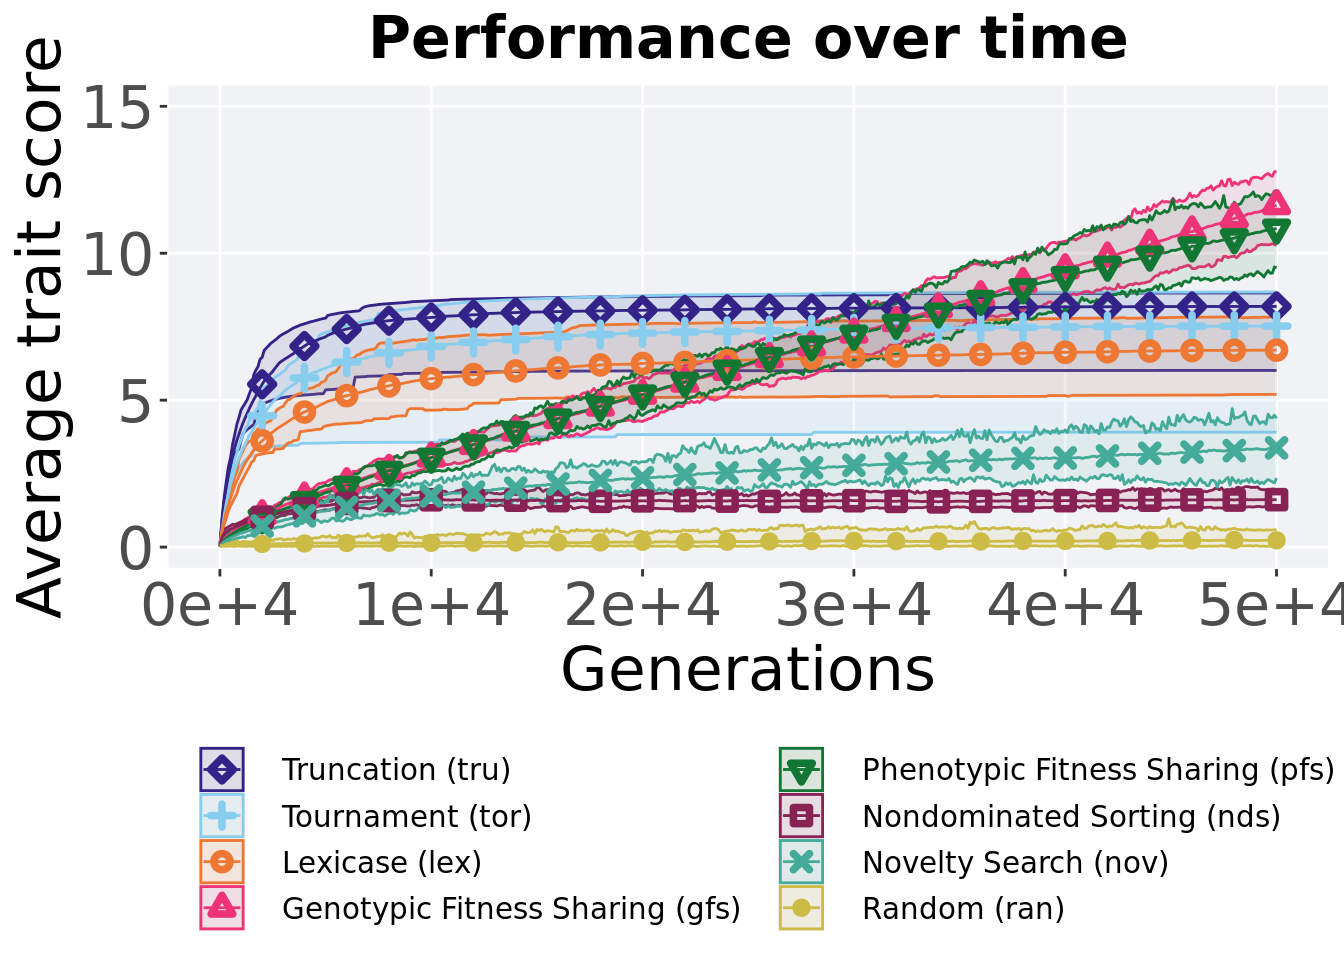
\includegraphics{demo_files/figure-latex/ord-mvc-per-ot-1.pdf}

\hypertarget{best-performance-throughout-3}{%
\subsection{Best performance throughout}\label{best-performance-throughout-3}}

Best performance found throughout 50,000 generations.

\begin{Shaded}
\begin{Highlighting}[]
\CommentTok{### best performance throughout}
\KeywordTok{filter}\NormalTok{(cc_best_mvc, col }\OperatorTok{==}\StringTok{ 'pop_fit_max'} \OperatorTok{&}\StringTok{ }\NormalTok{diagnostic }\OperatorTok{==}\StringTok{ 'ordered_exploitation'}\NormalTok{) }\OperatorTok
\StringTok{  }\KeywordTok{ggplot}\NormalTok{(., }\KeywordTok{aes}\NormalTok{(}\DataTypeTok{x =}\NormalTok{ acron, }\DataTypeTok{y =}\NormalTok{ val }\OperatorTok{/}\StringTok{ }\NormalTok{DIMENSIONALITY, }\DataTypeTok{color =}\NormalTok{ acron, }\DataTypeTok{fill =}\NormalTok{ acron, }\DataTypeTok{shape =}\NormalTok{ acron)) }\OperatorTok{+}
\StringTok{  }\KeywordTok{geom_flat_violin}\NormalTok{(}\DataTypeTok{position =} \KeywordTok{position_nudge}\NormalTok{(}\DataTypeTok{x =} \FloatTok{.2}\NormalTok{, }\DataTypeTok{y =} \DecValTok{0}\NormalTok{), }\DataTypeTok{scale =} \StringTok{'width'}\NormalTok{, }\DataTypeTok{alpha =} \FloatTok{0.2}\NormalTok{) }\OperatorTok{+}
\StringTok{  }\KeywordTok{geom_point}\NormalTok{(}\DataTypeTok{position =} \KeywordTok{position_jitter}\NormalTok{(}\DataTypeTok{width =} \FloatTok{.1}\NormalTok{), }\DataTypeTok{size =} \FloatTok{1.5}\NormalTok{, }\DataTypeTok{alpha =} \FloatTok{1.0}\NormalTok{) }\OperatorTok{+}
\StringTok{  }\KeywordTok{geom_boxplot}\NormalTok{(}\DataTypeTok{color =} \StringTok{'black'}\NormalTok{, }\DataTypeTok{width =} \FloatTok{.2}\NormalTok{, }\DataTypeTok{outlier.shape =} \OtherTok{NA}\NormalTok{, }\DataTypeTok{alpha =} \FloatTok{0.0}\NormalTok{) }\OperatorTok{+}
\StringTok{  }\KeywordTok{guides}\NormalTok{(}\DataTypeTok{fill =} \StringTok{"none"}\NormalTok{,}\DataTypeTok{color =} \StringTok{'none'}\NormalTok{, }\DataTypeTok{shape =} \StringTok{'none'}\NormalTok{) }\OperatorTok{+}
\StringTok{  }\KeywordTok{scale_y_continuous}\NormalTok{(}
    \DataTypeTok{name=}\StringTok{"Average trait score"}\NormalTok{,}
    \DataTypeTok{limits=}\KeywordTok{c}\NormalTok{(}\DecValTok{0}\NormalTok{, }\DecValTok{15}\NormalTok{),}
    \DataTypeTok{breaks=}\KeywordTok{seq}\NormalTok{(}\DecValTok{0}\NormalTok{,}\DecValTok{15}\NormalTok{, }\DecValTok{5}\NormalTok{),}
    \DataTypeTok{labels=}\KeywordTok{c}\NormalTok{(}\StringTok{"0"}\NormalTok{, }\StringTok{"5"}\NormalTok{, }\StringTok{"10"}\NormalTok{, }\StringTok{"15"}\NormalTok{)}
\NormalTok{  ) }\OperatorTok{+}
\StringTok{  }\KeywordTok{scale_x_discrete}\NormalTok{(}
    \DataTypeTok{name=}\StringTok{"Scheme"}
\NormalTok{  )}\OperatorTok{+}
\StringTok{  }\KeywordTok{scale_shape_manual}\NormalTok{(}\DataTypeTok{values=}\NormalTok{SHAPE)}\OperatorTok{+}
\StringTok{  }\KeywordTok{scale_colour_manual}\NormalTok{(}\DataTypeTok{values =}\NormalTok{ cb_palette, ) }\OperatorTok{+}
\StringTok{  }\KeywordTok{scale_fill_manual}\NormalTok{(}\DataTypeTok{values =}\NormalTok{ cb_palette) }\OperatorTok{+}
\StringTok{  }\KeywordTok{ggtitle}\NormalTok{(}\StringTok{'Best performance throughout'}\NormalTok{)}\OperatorTok{+}
\StringTok{  }\NormalTok{p_theme }\OperatorTok{+}\StringTok{ }\KeywordTok{theme}\NormalTok{(}\DataTypeTok{legend.title=}\KeywordTok{element_blank}\NormalTok{()) }\OperatorTok{+}
\StringTok{  }\KeywordTok{guides}\NormalTok{(}
    \DataTypeTok{shape=}\KeywordTok{guide_legend}\NormalTok{(}\DataTypeTok{nrow=}\DecValTok{2}\NormalTok{, }\DataTypeTok{title.position =} \StringTok{"bottom"}\NormalTok{),}
    \DataTypeTok{color=}\KeywordTok{guide_legend}\NormalTok{(}\DataTypeTok{nrow=}\DecValTok{2}\NormalTok{, }\DataTypeTok{title.position =} \StringTok{"bottom"}\NormalTok{),}
    \DataTypeTok{fill=}\KeywordTok{guide_legend}\NormalTok{(}\DataTypeTok{nrow=}\DecValTok{2}\NormalTok{, }\DataTypeTok{title.position =} \StringTok{"bottom"}\NormalTok{)}
\NormalTok{  )}
\end{Highlighting}
\end{Shaded}

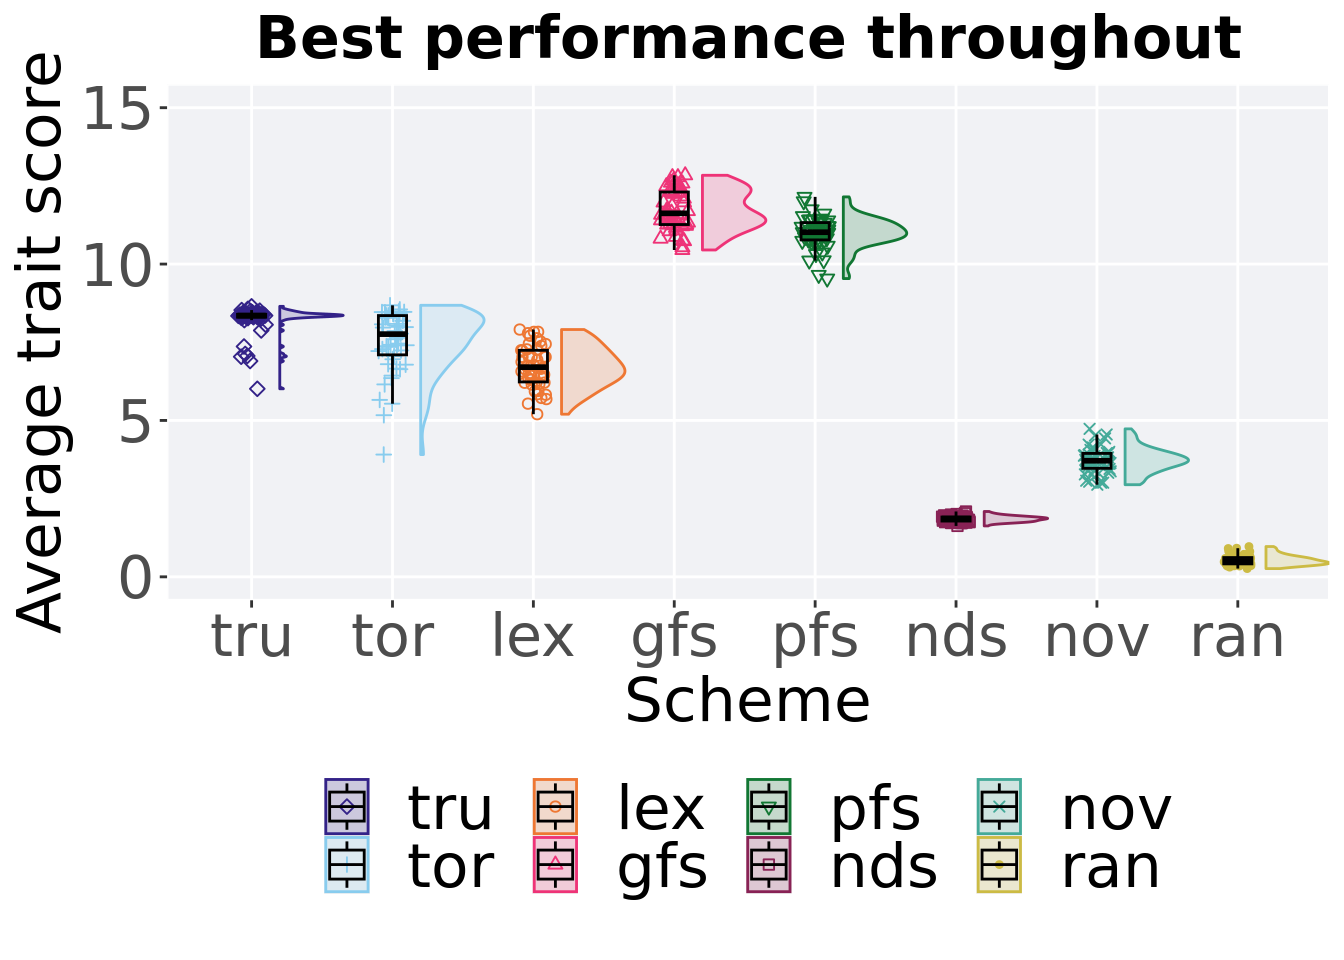
\includegraphics{demo_files/figure-latex/ord-mvc-per-bst-1.pdf}

\hypertarget{stats-6}{%
\subsubsection{Stats}\label{stats-6}}

Summary statistics for the performance of the best performance.

\begin{Shaded}
\begin{Highlighting}[]
\CommentTok{#get data & summarize}
\NormalTok{performance =}\StringTok{ }\KeywordTok{filter}\NormalTok{(cc_best_mvc, col }\OperatorTok{==}\StringTok{ 'pop_fit_max'} \OperatorTok{&}\StringTok{ }\NormalTok{diagnostic }\OperatorTok{==}\StringTok{ 'ordered_exploitation'}\NormalTok{)}
\NormalTok{performance}\OperatorTok{$}\NormalTok{acron =}\StringTok{ }\KeywordTok{factor}\NormalTok{(performance}\OperatorTok{$}\NormalTok{acron, }\DataTypeTok{levels =} \KeywordTok{c}\NormalTok{(}\StringTok{'gfs'}\NormalTok{,}\StringTok{'pfs'}\NormalTok{,}\StringTok{'tru'}\NormalTok{,}\StringTok{'tor'}\NormalTok{,}\StringTok{'lex'}\NormalTok{,}\StringTok{'nov'}\NormalTok{, }\StringTok{'nds'}\NormalTok{, }\StringTok{'ran'}\NormalTok{))}
\NormalTok{performance }\OperatorTok
\StringTok{  }\KeywordTok{group_by}\NormalTok{(acron) }\OperatorTok
\StringTok{  }\NormalTok{dplyr}\OperatorTok{::}\KeywordTok{summarise}\NormalTok{(}
    \DataTypeTok{count =} \KeywordTok{n}\NormalTok{(),}
    \DataTypeTok{na_cnt =} \KeywordTok{sum}\NormalTok{(}\KeywordTok{is.na}\NormalTok{(val)),}
    \DataTypeTok{min =} \KeywordTok{min}\NormalTok{(val }\OperatorTok{/}\StringTok{ }\NormalTok{DIMENSIONALITY, }\DataTypeTok{na.rm =} \OtherTok{TRUE}\NormalTok{),}
    \DataTypeTok{median =} \KeywordTok{median}\NormalTok{(val }\OperatorTok{/}\StringTok{ }\NormalTok{DIMENSIONALITY, }\DataTypeTok{na.rm =} \OtherTok{TRUE}\NormalTok{),}
    \DataTypeTok{mean =} \KeywordTok{mean}\NormalTok{(val }\OperatorTok{/}\StringTok{ }\NormalTok{DIMENSIONALITY, }\DataTypeTok{na.rm =} \OtherTok{TRUE}\NormalTok{),}
    \DataTypeTok{max =} \KeywordTok{max}\NormalTok{(val }\OperatorTok{/}\StringTok{ }\NormalTok{DIMENSIONALITY, }\DataTypeTok{na.rm =} \OtherTok{TRUE}\NormalTok{),}
    \DataTypeTok{IQR =} \KeywordTok{IQR}\NormalTok{(val }\OperatorTok{/}\StringTok{ }\NormalTok{DIMENSIONALITY, }\DataTypeTok{na.rm =} \OtherTok{TRUE}\NormalTok{)}
\NormalTok{  )}
\end{Highlighting}
\end{Shaded}

\begin{verbatim}
## # A tibble: 8 x 8
##   acron count na_cnt    min median   mean    max    IQR
##   <fct> <int>  <int>  <dbl>  <dbl>  <dbl>  <dbl>  <dbl>
## 1 gfs      50      0 10.5   11.6   11.7   12.8   1.04  
## 2 pfs      50      0  9.54  11.0   11.0   12.1   0.553 
## 3 tru      50      0  6.01   8.35   8.19   8.65  0.0922
## 4 tor      50      0  3.91   7.76   7.52   8.68  1.26  
## 5 lex      50      0  5.20   6.70   6.72   7.91  1.01  
## 6 nov      50      0  2.95   3.71   3.72   4.73  0.476 
## 7 nds      50      0  1.63   1.86   1.85   2.09  0.129 
## 8 ran      50      0  0.263  0.490  0.534  0.968 0.202
\end{verbatim}

Kruskal--Wallis test provides evidence of statistical differences.

\begin{Shaded}
\begin{Highlighting}[]
\KeywordTok{kruskal.test}\NormalTok{(val }\OperatorTok{~}\StringTok{ }\NormalTok{acron, }\DataTypeTok{data =}\NormalTok{ performance)}
\end{Highlighting}
\end{Shaded}

\begin{verbatim}
## 
##  Kruskal-Wallis rank sum test
## 
## data:  val by acron
## Kruskal-Wallis chi-squared = 380.23, df = 7, p-value < 2.2e-16
\end{verbatim}

Results for post-hoc Wilcoxon rank-sum test with a Bonferroni correction.

\begin{Shaded}
\begin{Highlighting}[]
\KeywordTok{pairwise.wilcox.test}\NormalTok{(}\DataTypeTok{x =}\NormalTok{ performance}\OperatorTok{$}\NormalTok{val, }\DataTypeTok{g =}\NormalTok{ performance}\OperatorTok{$}\NormalTok{acron, }\DataTypeTok{p.adjust.method =} \StringTok{"bonferroni"}\NormalTok{,}
                     \DataTypeTok{paired =} \OtherTok{FALSE}\NormalTok{, }\DataTypeTok{conf.int =} \OtherTok{FALSE}\NormalTok{, }\DataTypeTok{alternative =} \StringTok{'l'}\NormalTok{)}
\end{Highlighting}
\end{Shaded}

\begin{verbatim}
## 
##  Pairwise comparisons using Wilcoxon rank sum test with continuity correction 
## 
## data:  performance$val and performance$acron 
## 
##     gfs     pfs     tru     tor     lex     nov     nds    
## pfs 1.6e-06 -       -       -       -       -       -      
## tru < 2e-16 < 2e-16 -       -       -       -       -      
## tor < 2e-16 < 2e-16 0.0026  -       -       -       -      
## lex < 2e-16 < 2e-16 7.7e-14 1.7e-05 -       -       -      
## nov < 2e-16 < 2e-16 < 2e-16 2.4e-16 < 2e-16 -       -      
## nds < 2e-16 < 2e-16 < 2e-16 < 2e-16 < 2e-16 < 2e-16 -      
## ran < 2e-16 < 2e-16 < 2e-16 < 2e-16 < 2e-16 < 2e-16 < 2e-16
## 
## P value adjustment method: bonferroni
\end{verbatim}

\hypertarget{performance-comparison-1}{%
\subsection{Performance comparison}\label{performance-comparison-1}}

Best performances in the population at 40,000 and 50,000 generations.

\begin{verbatim}
## Warning: The following aesthetics were dropped during statistical transformation:
## colour, shape
## i This can happen when ggplot fails to infer the correct grouping structure in
##   the data.
## i Did you forget to specify a `group` aesthetic or to convert a numerical
##   variable into a factor?
## The following aesthetics were dropped during statistical transformation:
## colour, shape
## i This can happen when ggplot fails to infer the correct grouping structure in
##   the data.
## i Did you forget to specify a `group` aesthetic or to convert a numerical
##   variable into a factor?
\end{verbatim}

\begin{Shaded}
\begin{Highlighting}[]
\CommentTok{# 80% and final generation comparison}
\NormalTok{end =}\StringTok{ }\KeywordTok{filter}\NormalTok{(cc_over_time_mvc, diagnostic }\OperatorTok{==}\StringTok{ 'ordered_exploitation'} \OperatorTok{&}\StringTok{ }\NormalTok{gen }\OperatorTok{==}\StringTok{ }\DecValTok{50000} \OperatorTok{&}\StringTok{ }\NormalTok{acron }\OperatorTok{!=}\StringTok{ 'ran'}\NormalTok{)}
\NormalTok{end}\OperatorTok{$}\NormalTok{Generation <-}\StringTok{ }\KeywordTok{factor}\NormalTok{(end}\OperatorTok{$}\NormalTok{gen)}

\NormalTok{mid =}\StringTok{ }\KeywordTok{filter}\NormalTok{(cc_over_time_mvc, diagnostic }\OperatorTok{==}\StringTok{ 'ordered_exploitation'} \OperatorTok{&}\StringTok{ }\NormalTok{gen }\OperatorTok{==}\StringTok{ }\DecValTok{40000} \OperatorTok{&}\StringTok{ }\NormalTok{acron }\OperatorTok{!=}\StringTok{ 'ran'}\NormalTok{)}
\NormalTok{mid}\OperatorTok{$}\NormalTok{Generation <-}\StringTok{ }\KeywordTok{factor}\NormalTok{(mid}\OperatorTok{$}\NormalTok{gen)}

\NormalTok{mvc_p =}\StringTok{ }\KeywordTok{ggplot}\NormalTok{(mid, }\KeywordTok{aes}\NormalTok{(}\DataTypeTok{x =}\NormalTok{ acron, }\DataTypeTok{y=}\NormalTok{pop_fit_max }\OperatorTok{/}\StringTok{ }\NormalTok{DIMENSIONALITY, }\DataTypeTok{group =}\NormalTok{ acron, }\DataTypeTok{shape =}\NormalTok{ Generation)) }\OperatorTok{+}
\StringTok{  }\KeywordTok{geom_point}\NormalTok{(}\DataTypeTok{col =}\NormalTok{ mvc_col[}\DecValTok{1}\NormalTok{] , }\DataTypeTok{position =} \KeywordTok{position_jitternudge}\NormalTok{(}\DataTypeTok{jitter.width =} \FloatTok{.03}\NormalTok{, }\DataTypeTok{nudge.x =} \FloatTok{-0.05}\NormalTok{), }\DataTypeTok{size =} \DecValTok{2}\NormalTok{, }\DataTypeTok{alpha =} \FloatTok{1.0}\NormalTok{) }\OperatorTok{+}
\StringTok{  }\KeywordTok{geom_boxplot}\NormalTok{(}\DataTypeTok{position =} \KeywordTok{position_nudge}\NormalTok{(}\DataTypeTok{x =} \FloatTok{-.15}\NormalTok{, }\DataTypeTok{y =} \DecValTok{0}\NormalTok{), }\DataTypeTok{lwd =} \FloatTok{0.7}\NormalTok{, }\DataTypeTok{col =}\NormalTok{ mvc_col[}\DecValTok{1}\NormalTok{], }\DataTypeTok{fill =}\NormalTok{ mvc_col[}\DecValTok{1}\NormalTok{], }\DataTypeTok{width =} \FloatTok{.1}\NormalTok{, }\DataTypeTok{outlier.shape =} \OtherTok{NA}\NormalTok{, }\DataTypeTok{alpha =} \FloatTok{0.0}\NormalTok{) }\OperatorTok{+}

\StringTok{  }\KeywordTok{geom_point}\NormalTok{(}\DataTypeTok{data =}\NormalTok{ end, }\KeywordTok{aes}\NormalTok{(}\DataTypeTok{x =}\NormalTok{ acron, }\DataTypeTok{y=}\NormalTok{pop_fit_max }\OperatorTok{/}\StringTok{ }\NormalTok{DIMENSIONALITY), }\DataTypeTok{col =}\NormalTok{ mvc_col[}\DecValTok{2}\NormalTok{], }\DataTypeTok{position =} \KeywordTok{position_jitternudge}\NormalTok{(}\DataTypeTok{jitter.width =} \FloatTok{.03}\NormalTok{, }\DataTypeTok{nudge.x =} \FloatTok{0.05}\NormalTok{), }\DataTypeTok{size =} \DecValTok{2}\NormalTok{, }\DataTypeTok{alpha =} \FloatTok{1.0}\NormalTok{) }\OperatorTok{+}
\StringTok{  }\KeywordTok{geom_boxplot}\NormalTok{(}\DataTypeTok{data =}\NormalTok{ end, }\KeywordTok{aes}\NormalTok{(}\DataTypeTok{x =}\NormalTok{ acron, }\DataTypeTok{y=}\NormalTok{pop_fit_max }\OperatorTok{/}\StringTok{ }\NormalTok{DIMENSIONALITY), }\DataTypeTok{position =} \KeywordTok{position_nudge}\NormalTok{(}\DataTypeTok{x =} \FloatTok{.15}\NormalTok{, }\DataTypeTok{y =} \DecValTok{0}\NormalTok{), }\DataTypeTok{lwd =} \FloatTok{0.7}\NormalTok{, }\DataTypeTok{col =}\NormalTok{ mvc_col[}\DecValTok{2}\NormalTok{], }\DataTypeTok{fill =}\NormalTok{ mvc_col[}\DecValTok{2}\NormalTok{], }\DataTypeTok{width =} \FloatTok{.1}\NormalTok{, }\DataTypeTok{outlier.shape =} \OtherTok{NA}\NormalTok{, }\DataTypeTok{alpha =} \FloatTok{0.0}\NormalTok{) }\OperatorTok{+}

\StringTok{  }\KeywordTok{scale_y_continuous}\NormalTok{(}
    \DataTypeTok{name=}\StringTok{"Average trait score"}\NormalTok{,}
    \DataTypeTok{limits=}\KeywordTok{c}\NormalTok{(}\DecValTok{0}\NormalTok{, }\DecValTok{15}\NormalTok{),}
    \DataTypeTok{breaks=}\KeywordTok{seq}\NormalTok{(}\DecValTok{0}\NormalTok{,}\DecValTok{15}\NormalTok{, }\DecValTok{5}\NormalTok{),}
    \DataTypeTok{labels=}\KeywordTok{c}\NormalTok{(}\StringTok{"0"}\NormalTok{, }\StringTok{"5"}\NormalTok{, }\StringTok{"10"}\NormalTok{, }\StringTok{"15"}\NormalTok{)}
\NormalTok{  ) }\OperatorTok{+}
\StringTok{  }\KeywordTok{scale_x_discrete}\NormalTok{(}
    \DataTypeTok{name=}\StringTok{"Scheme"}
\NormalTok{  )}\OperatorTok{+}
\StringTok{  }\KeywordTok{scale_shape_manual}\NormalTok{(}\DataTypeTok{values=}\KeywordTok{c}\NormalTok{(}\DecValTok{0}\NormalTok{,}\DecValTok{1}\NormalTok{))}\OperatorTok{+}
\StringTok{  }\KeywordTok{scale_colour_manual}\NormalTok{(}\DataTypeTok{values =} \KeywordTok{c}\NormalTok{(mvc_col[}\DecValTok{1}\NormalTok{],mvc_col[}\DecValTok{2}\NormalTok{])) }\OperatorTok{+}
\StringTok{  }\NormalTok{p_theme}

\KeywordTok{plot_grid}\NormalTok{(}
\NormalTok{  mvc_p }\OperatorTok{+}
\StringTok{    }\KeywordTok{ggtitle}\NormalTok{(}\StringTok{"Performance comparisons"}\NormalTok{) }\OperatorTok{+}
\StringTok{    }\KeywordTok{theme}\NormalTok{(}\DataTypeTok{legend.position=}\StringTok{"none"}\NormalTok{),}
\NormalTok{  legend,}
  \DataTypeTok{nrow=}\DecValTok{2}\NormalTok{,}
  \DataTypeTok{rel_heights =} \KeywordTok{c}\NormalTok{(}\DecValTok{1}\NormalTok{,.}\DecValTok{05}\NormalTok{),}
  \DataTypeTok{label_size =}\NormalTok{ TSIZE}
\NormalTok{)}
\end{Highlighting}
\end{Shaded}

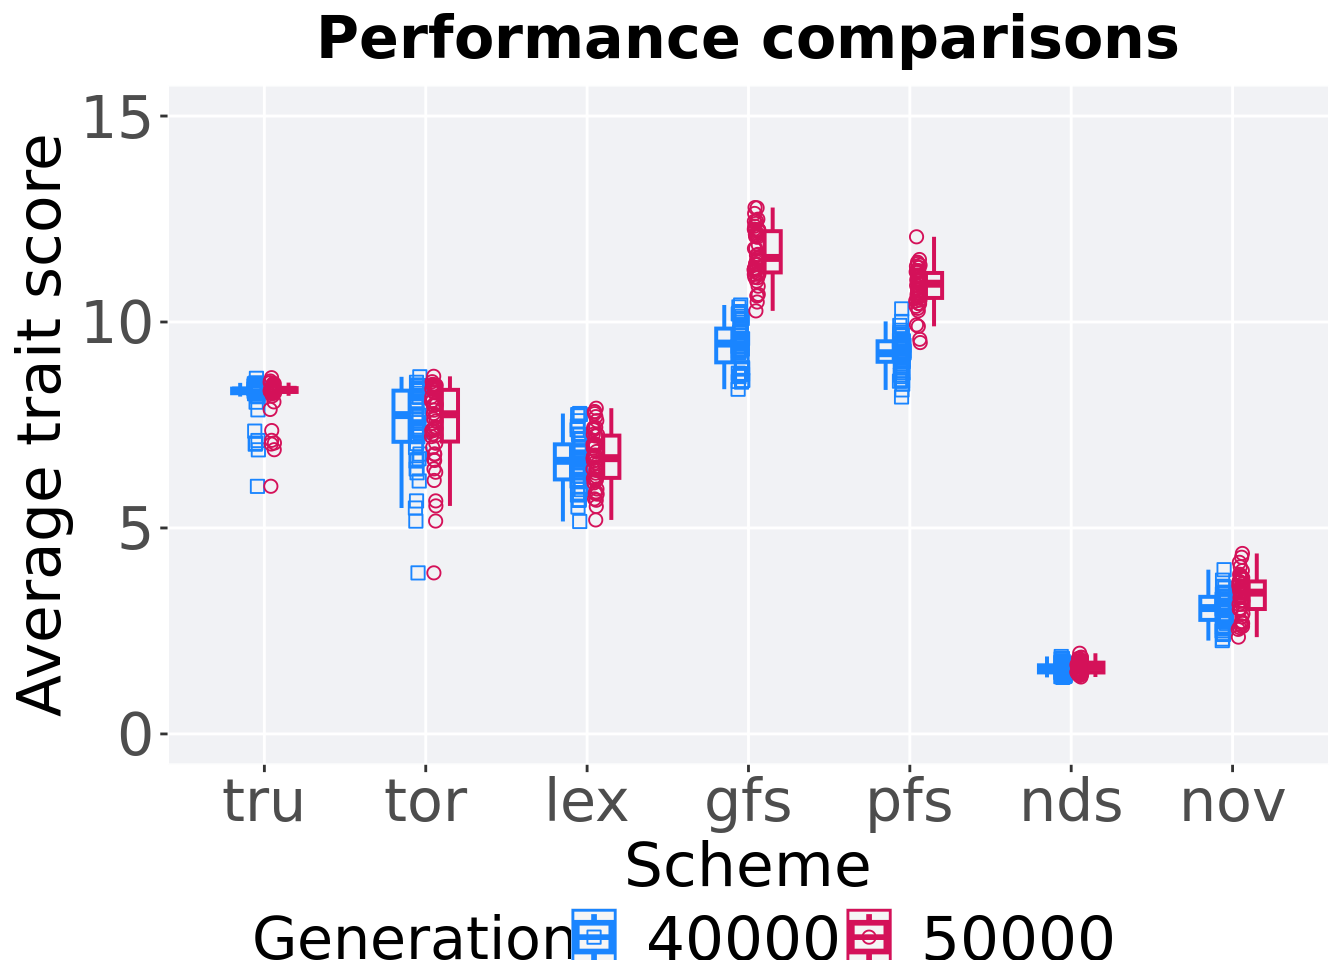
\includegraphics{demo_files/figure-latex/ord-mvc-per-sli-1.pdf}

\hypertarget{stats-7}{%
\subsubsection{Stats}\label{stats-7}}

Summary statistics for the performance of the best performance at 40,000 and 50,000 generations.

\begin{Shaded}
\begin{Highlighting}[]
\CommentTok{### performance comparisons and generation slices 40K & 50K}
\NormalTok{slices =}\StringTok{ }\KeywordTok{filter}\NormalTok{(cc_over_time_mvc, diagnostic }\OperatorTok{==}\StringTok{ 'ordered_exploitation'} \OperatorTok{&}\StringTok{ }\NormalTok{(gen }\OperatorTok{==}\StringTok{ }\DecValTok{50000} \OperatorTok{|}\StringTok{ }\NormalTok{gen }\OperatorTok{==}\StringTok{ }\DecValTok{40000}\NormalTok{) }\OperatorTok{&}\StringTok{ }\NormalTok{acron }\OperatorTok{!=}\StringTok{ 'ran'}\NormalTok{)}
\NormalTok{slices}\OperatorTok{$}\NormalTok{Generation <-}\StringTok{ }\KeywordTok{factor}\NormalTok{(slices}\OperatorTok{$}\NormalTok{gen, }\DataTypeTok{levels =} \KeywordTok{c}\NormalTok{(}\DecValTok{50000}\NormalTok{,}\DecValTok{40000}\NormalTok{))}
\NormalTok{slices}\OperatorTok{$}\NormalTok{acron =}\StringTok{ }\KeywordTok{factor}\NormalTok{(slices}\OperatorTok{$}\NormalTok{acron, }\DataTypeTok{levels =} \KeywordTok{c}\NormalTok{(}\StringTok{'gfs'}\NormalTok{,}\StringTok{'pfs'}\NormalTok{,}\StringTok{'tru'}\NormalTok{,}\StringTok{'tor'}\NormalTok{,}\StringTok{'lex'}\NormalTok{,}\StringTok{'nov'}\NormalTok{, }\StringTok{'nds'}\NormalTok{, }\StringTok{'ran'}\NormalTok{))}
\NormalTok{slices }\OperatorTok
\StringTok{  }\KeywordTok{group_by}\NormalTok{(acron, Generation) }\OperatorTok
\StringTok{  }\NormalTok{dplyr}\OperatorTok{::}\KeywordTok{summarise}\NormalTok{(}
    \DataTypeTok{count =} \KeywordTok{n}\NormalTok{(),}
    \DataTypeTok{na_cnt =} \KeywordTok{sum}\NormalTok{(}\KeywordTok{is.na}\NormalTok{(pop_fit_max  }\OperatorTok{/}\StringTok{ }\NormalTok{DIMENSIONALITY)),}
    \DataTypeTok{min =} \KeywordTok{min}\NormalTok{(pop_fit_max  }\OperatorTok{/}\StringTok{ }\NormalTok{DIMENSIONALITY, }\DataTypeTok{na.rm =} \OtherTok{TRUE}\NormalTok{),}
    \DataTypeTok{median =} \KeywordTok{median}\NormalTok{(pop_fit_max  }\OperatorTok{/}\StringTok{ }\NormalTok{DIMENSIONALITY, }\DataTypeTok{na.rm =} \OtherTok{TRUE}\NormalTok{),}
    \DataTypeTok{mean =} \KeywordTok{mean}\NormalTok{(pop_fit_max  }\OperatorTok{/}\StringTok{ }\NormalTok{DIMENSIONALITY, }\DataTypeTok{na.rm =} \OtherTok{TRUE}\NormalTok{),}
    \DataTypeTok{max =} \KeywordTok{max}\NormalTok{(pop_fit_max  }\OperatorTok{/}\StringTok{ }\NormalTok{DIMENSIONALITY, }\DataTypeTok{na.rm =} \OtherTok{TRUE}\NormalTok{),}
    \DataTypeTok{IQR =} \KeywordTok{IQR}\NormalTok{(pop_fit_max  }\OperatorTok{/}\StringTok{ }\NormalTok{DIMENSIONALITY, }\DataTypeTok{na.rm =} \OtherTok{TRUE}\NormalTok{)}
\NormalTok{  )}
\end{Highlighting}
\end{Shaded}

\begin{verbatim}
## `summarise()` has grouped output by 'acron'. You can override using the
## `.groups` argument.
\end{verbatim}

\begin{verbatim}
## # A tibble: 14 x 9
## # Groups:   acron [7]
##    acron Generation count na_cnt   min median  mean   max    IQR
##    <fct> <fct>      <int>  <int> <dbl>  <dbl> <dbl> <dbl>  <dbl>
##  1 gfs   50000         50      0 10.3   11.6  11.6  12.8  1.00  
##  2 gfs   40000         50      0  8.37   9.48  9.45 10.4  0.820 
##  3 pfs   50000         50      0  9.50  10.9  10.8  12.1  0.606 
##  4 pfs   40000         50      0  8.18   9.24  9.23 10.3  0.498 
##  5 tru   50000         50      0  6.01   8.35  8.19  8.65 0.0922
##  6 tru   40000         50      0  6.01   8.33  8.17  8.63 0.112 
##  7 tor   50000         50      0  3.91   7.76  7.52  8.68 1.26  
##  8 tor   40000         50      0  3.91   7.74  7.49  8.67 1.24  
##  9 lex   50000         50      0  5.19   6.69  6.70  7.91 1.03  
## 10 lex   40000         50      0  5.16   6.63  6.63  7.78 0.852 
## 11 nov   50000         50      0  2.35   3.43  3.38  4.38 0.670 
## 12 nov   40000         50      0  2.27   3.06  3.03  3.99 0.560 
## 13 nds   50000         50      0  1.38   1.63  1.61  1.96 0.239 
## 14 nds   40000         50      0  1.37   1.58  1.58  1.88 0.173
\end{verbatim}

Truncation selection comparisons.

\begin{Shaded}
\begin{Highlighting}[]
\KeywordTok{wilcox.test}\NormalTok{(}\DataTypeTok{x =} \KeywordTok{filter}\NormalTok{(slices, acron }\OperatorTok{==}\StringTok{ 'tru'} \OperatorTok{&}\StringTok{ }\NormalTok{Generation }\OperatorTok{==}\StringTok{ }\DecValTok{50000}\NormalTok{)}\OperatorTok{$}\NormalTok{pop_fit_max,}
            \DataTypeTok{y =} \KeywordTok{filter}\NormalTok{(slices, acron }\OperatorTok{==}\StringTok{ 'tru'} \OperatorTok{&}\StringTok{ }\NormalTok{Generation }\OperatorTok{==}\StringTok{ }\DecValTok{40000}\NormalTok{)}\OperatorTok{$}\NormalTok{pop_fit_max,}
            \DataTypeTok{alternative =} \StringTok{'t'}\NormalTok{)}
\end{Highlighting}
\end{Shaded}

\begin{verbatim}
## 
##  Wilcoxon rank sum test with continuity correction
## 
## data:  filter(slices, acron == "tru" & Generation == 50000)$pop_fit_max and filter(slices, acron == "tru" & Generation == 40000)$pop_fit_max
## W = 1375, p-value = 0.3907
## alternative hypothesis: true location shift is not equal to 0
\end{verbatim}

Tournament selection comparisons.

\begin{Shaded}
\begin{Highlighting}[]
\KeywordTok{wilcox.test}\NormalTok{(}\DataTypeTok{x =} \KeywordTok{filter}\NormalTok{(slices, acron }\OperatorTok{==}\StringTok{ 'tor'} \OperatorTok{&}\StringTok{ }\NormalTok{Generation }\OperatorTok{==}\StringTok{ }\DecValTok{50000}\NormalTok{)}\OperatorTok{$}\NormalTok{pop_fit_max,}
            \DataTypeTok{y =} \KeywordTok{filter}\NormalTok{(slices, acron }\OperatorTok{==}\StringTok{ 'tor'} \OperatorTok{&}\StringTok{ }\NormalTok{Generation }\OperatorTok{==}\StringTok{ }\DecValTok{40000}\NormalTok{)}\OperatorTok{$}\NormalTok{pop_fit_max,}
            \DataTypeTok{alternative =} \StringTok{'t'}\NormalTok{)}
\end{Highlighting}
\end{Shaded}

\begin{verbatim}
## 
##  Wilcoxon rank sum test with continuity correction
## 
## data:  filter(slices, acron == "tor" & Generation == 50000)$pop_fit_max and filter(slices, acron == "tor" & Generation == 40000)$pop_fit_max
## W = 1306.5, p-value = 0.6995
## alternative hypothesis: true location shift is not equal to 0
\end{verbatim}

Lexicase selection comparisons.

\begin{Shaded}
\begin{Highlighting}[]
\KeywordTok{wilcox.test}\NormalTok{(}\DataTypeTok{x =} \KeywordTok{filter}\NormalTok{(slices, acron }\OperatorTok{==}\StringTok{ 'lex'} \OperatorTok{&}\StringTok{ }\NormalTok{Generation }\OperatorTok{==}\StringTok{ }\DecValTok{50000}\NormalTok{)}\OperatorTok{$}\NormalTok{pop_fit_max,}
            \DataTypeTok{y =} \KeywordTok{filter}\NormalTok{(slices, acron }\OperatorTok{==}\StringTok{ 'lex'} \OperatorTok{&}\StringTok{ }\NormalTok{Generation }\OperatorTok{==}\StringTok{ }\DecValTok{40000}\NormalTok{)}\OperatorTok{$}\NormalTok{pop_fit_max,}
            \DataTypeTok{alternative =} \StringTok{'t'}\NormalTok{)}
\end{Highlighting}
\end{Shaded}

\begin{verbatim}
## 
##  Wilcoxon rank sum test with continuity correction
## 
## data:  filter(slices, acron == "lex" & Generation == 50000)$pop_fit_max and filter(slices, acron == "lex" & Generation == 40000)$pop_fit_max
## W = 1348, p-value = 0.5015
## alternative hypothesis: true location shift is not equal to 0
\end{verbatim}

Genotypic fitness sharing comparisons.

\begin{Shaded}
\begin{Highlighting}[]
\KeywordTok{wilcox.test}\NormalTok{(}\DataTypeTok{x =} \KeywordTok{filter}\NormalTok{(slices, acron }\OperatorTok{==}\StringTok{ 'gfs'} \OperatorTok{&}\StringTok{ }\NormalTok{Generation }\OperatorTok{==}\StringTok{ }\DecValTok{50000}\NormalTok{)}\OperatorTok{$}\NormalTok{pop_fit_max,}
            \DataTypeTok{y =} \KeywordTok{filter}\NormalTok{(slices, acron }\OperatorTok{==}\StringTok{ 'gfs'} \OperatorTok{&}\StringTok{ }\NormalTok{Generation }\OperatorTok{==}\StringTok{ }\DecValTok{40000}\NormalTok{)}\OperatorTok{$}\NormalTok{pop_fit_max,}
            \DataTypeTok{alternative =} \StringTok{'t'}\NormalTok{)}
\end{Highlighting}
\end{Shaded}

\begin{verbatim}
## 
##  Wilcoxon rank sum test with continuity correction
## 
## data:  filter(slices, acron == "gfs" & Generation == 50000)$pop_fit_max and filter(slices, acron == "gfs" & Generation == 40000)$pop_fit_max
## W = 2498, p-value < 2.2e-16
## alternative hypothesis: true location shift is not equal to 0
\end{verbatim}

Phenotypic fitness sharing comparisons.

\begin{Shaded}
\begin{Highlighting}[]
\KeywordTok{wilcox.test}\NormalTok{(}\DataTypeTok{x =} \KeywordTok{filter}\NormalTok{(slices, acron }\OperatorTok{==}\StringTok{ 'pfs'} \OperatorTok{&}\StringTok{ }\NormalTok{Generation }\OperatorTok{==}\StringTok{ }\DecValTok{50000}\NormalTok{)}\OperatorTok{$}\NormalTok{pop_fit_max,}
            \DataTypeTok{y =} \KeywordTok{filter}\NormalTok{(slices, acron }\OperatorTok{==}\StringTok{ 'pfs'} \OperatorTok{&}\StringTok{ }\NormalTok{Generation }\OperatorTok{==}\StringTok{ }\DecValTok{40000}\NormalTok{)}\OperatorTok{$}\NormalTok{pop_fit_max,}
            \DataTypeTok{alternative =} \StringTok{'t'}\NormalTok{)}
\end{Highlighting}
\end{Shaded}

\begin{verbatim}
## 
##  Wilcoxon rank sum test with continuity correction
## 
## data:  filter(slices, acron == "pfs" & Generation == 50000)$pop_fit_max and filter(slices, acron == "pfs" & Generation == 40000)$pop_fit_max
## W = 2471, p-value < 2.2e-16
## alternative hypothesis: true location shift is not equal to 0
\end{verbatim}

Nondominated sorting comparisons.

\begin{Shaded}
\begin{Highlighting}[]
\KeywordTok{wilcox.test}\NormalTok{(}\DataTypeTok{x =} \KeywordTok{filter}\NormalTok{(slices, acron }\OperatorTok{==}\StringTok{ 'nds'} \OperatorTok{&}\StringTok{ }\NormalTok{Generation }\OperatorTok{==}\StringTok{ }\DecValTok{50000}\NormalTok{)}\OperatorTok{$}\NormalTok{pop_fit_max,}
            \DataTypeTok{y =} \KeywordTok{filter}\NormalTok{(slices, acron }\OperatorTok{==}\StringTok{ 'nds'} \OperatorTok{&}\StringTok{ }\NormalTok{Generation }\OperatorTok{==}\StringTok{ }\DecValTok{40000}\NormalTok{)}\OperatorTok{$}\NormalTok{pop_fit_max,}
            \DataTypeTok{alternative =} \StringTok{'t'}\NormalTok{)}
\end{Highlighting}
\end{Shaded}

\begin{verbatim}
## 
##  Wilcoxon rank sum test with continuity correction
## 
## data:  filter(slices, acron == "nds" & Generation == 50000)$pop_fit_max and filter(slices, acron == "nds" & Generation == 40000)$pop_fit_max
## W = 1413, p-value = 0.2626
## alternative hypothesis: true location shift is not equal to 0
\end{verbatim}

Novelty search comparisons.

\begin{Shaded}
\begin{Highlighting}[]
\KeywordTok{wilcox.test}\NormalTok{(}\DataTypeTok{x =} \KeywordTok{filter}\NormalTok{(slices, acron }\OperatorTok{==}\StringTok{ 'nov'} \OperatorTok{&}\StringTok{ }\NormalTok{Generation }\OperatorTok{==}\StringTok{ }\DecValTok{50000}\NormalTok{)}\OperatorTok{$}\NormalTok{pop_fit_max,}
            \DataTypeTok{y =} \KeywordTok{filter}\NormalTok{(slices, acron }\OperatorTok{==}\StringTok{ 'nov'} \OperatorTok{&}\StringTok{ }\NormalTok{Generation }\OperatorTok{==}\StringTok{ }\DecValTok{40000}\NormalTok{)}\OperatorTok{$}\NormalTok{pop_fit_max,}
            \DataTypeTok{alternative =} \StringTok{'t'}\NormalTok{)}
\end{Highlighting}
\end{Shaded}

\begin{verbatim}
## 
##  Wilcoxon rank sum test with continuity correction
## 
## data:  filter(slices, acron == "nov" & Generation == 50000)$pop_fit_max and filter(slices, acron == "nov" & Generation == 40000)$pop_fit_max
## W = 1789, p-value = 0.0002054
## alternative hypothesis: true location shift is not equal to 0
\end{verbatim}

\hypertarget{contradictory-objectives-results}{%
\chapter{Contradictory objectives results}\label{contradictory-objectives-results}}

Here we present the results for the \textbf{satisfactory trait corverage} and \textbf{activation gene coverage} generated by each selection scheme replicate on the contradictory objectives diagnostic.
Note both of these values are gathered at the population-level.
Activation gene coverage refers to the count of unique activation genes in a given population; this gives us a range of integers between 0 and 100.
Satisfactory trait coverage refers to the count of unique satisfied traits in a given population; this gives us a range of integers between 0 and 100.

\hypertarget{analysis-dependencies-2}{%
\section{Analysis dependencies}\label{analysis-dependencies-2}}

\begin{Shaded}
\begin{Highlighting}[]
\KeywordTok{library}\NormalTok{(ggplot2)}
\KeywordTok{library}\NormalTok{(cowplot)}
\KeywordTok{library}\NormalTok{(dplyr)}
\KeywordTok{library}\NormalTok{(PupillometryR)}
\KeywordTok{library}\NormalTok{(sdamr)}
\end{Highlighting}
\end{Shaded}

\hypertarget{satisfactory-trait-coverage}{%
\section{Satisfactory trait coverage}\label{satisfactory-trait-coverage}}

Satisfactory trait coverage analysis.

\hypertarget{coverage-over-time}{%
\subsection{Coverage over time}\label{coverage-over-time}}

Satisfactory trait coverage over time.

\begin{Shaded}
\begin{Highlighting}[]
\CommentTok{# data for lines and shading on plots}
\NormalTok{lines =}\StringTok{ }\KeywordTok{filter}\NormalTok{(cc_over_time, diagnostic }\OperatorTok{==}\StringTok{ 'contradictory_objectives'}\NormalTok{) }\OperatorTok
\StringTok{  }\KeywordTok{group_by}\NormalTok{(}\StringTok{`}\DataTypeTok{Selection}\CharTok{\textbackslash{}n}\DataTypeTok{Scheme}\StringTok{`}\NormalTok{, gen) }\OperatorTok
\StringTok{  }\NormalTok{dplyr}\OperatorTok{::}\KeywordTok{summarise}\NormalTok{(}
    \DataTypeTok{min =} \KeywordTok{min}\NormalTok{(pop_uni_obj),}
    \DataTypeTok{mean =} \KeywordTok{mean}\NormalTok{(pop_uni_obj),}
    \DataTypeTok{max =} \KeywordTok{max}\NormalTok{(pop_uni_obj)}
\NormalTok{  )}
\end{Highlighting}
\end{Shaded}

\begin{verbatim}
## `summarise()` has grouped output by 'Selection Scheme'. You can override using
## the `.groups` argument.
\end{verbatim}

\begin{Shaded}
\begin{Highlighting}[]
\KeywordTok{ggplot}\NormalTok{(lines, }\KeywordTok{aes}\NormalTok{(}\DataTypeTok{x=}\NormalTok{gen, }\DataTypeTok{y=}\NormalTok{mean, }\DataTypeTok{group =} \StringTok{`}\DataTypeTok{Selection}\CharTok{\textbackslash{}n}\DataTypeTok{Scheme}\StringTok{`}\NormalTok{, }\DataTypeTok{fill =}\StringTok{`}\DataTypeTok{Selection}\CharTok{\textbackslash{}n}\DataTypeTok{Scheme}\StringTok{`}\NormalTok{, }\DataTypeTok{color =} \StringTok{`}\DataTypeTok{Selection}\CharTok{\textbackslash{}n}\DataTypeTok{Scheme}\StringTok{`}\NormalTok{, }\DataTypeTok{shape =} \StringTok{`}\DataTypeTok{Selection}\CharTok{\textbackslash{}n}\DataTypeTok{Scheme}\StringTok{`}\NormalTok{)) }\OperatorTok{+}
\StringTok{  }\KeywordTok{geom_ribbon}\NormalTok{(}\KeywordTok{aes}\NormalTok{(}\DataTypeTok{ymin =}\NormalTok{ min, }\DataTypeTok{ymax =}\NormalTok{ max), }\DataTypeTok{alpha =} \FloatTok{0.1}\NormalTok{) }\OperatorTok{+}
\StringTok{  }\KeywordTok{geom_line}\NormalTok{(}\DataTypeTok{size =} \FloatTok{0.5}\NormalTok{) }\OperatorTok{+}
\StringTok{  }\KeywordTok{geom_point}\NormalTok{(}\DataTypeTok{data =} \KeywordTok{filter}\NormalTok{(lines, gen }\OperatorTok\StringTok{ }\DecValTok{2000} \OperatorTok{==}\StringTok{ }\DecValTok{0} \OperatorTok{&}\StringTok{ }\NormalTok{gen }\OperatorTok{!=}\StringTok{ }\DecValTok{0}\NormalTok{), }\DataTypeTok{size =} \FloatTok{1.5}\NormalTok{, }\DataTypeTok{stroke =} \FloatTok{2.0}\NormalTok{, }\DataTypeTok{alpha =} \FloatTok{1.0}\NormalTok{) }\OperatorTok{+}
\StringTok{  }\KeywordTok{scale_y_continuous}\NormalTok{(}
    \DataTypeTok{name=}\StringTok{"Coverage"}\NormalTok{,}
    \DataTypeTok{limits=}\KeywordTok{c}\NormalTok{(}\DecValTok{0}\NormalTok{, }\DecValTok{100}\NormalTok{),}
    \DataTypeTok{breaks=}\KeywordTok{seq}\NormalTok{(}\DecValTok{0}\NormalTok{,}\DecValTok{100}\NormalTok{, }\DecValTok{20}\NormalTok{),}
    \DataTypeTok{labels=}\KeywordTok{c}\NormalTok{(}\StringTok{"0"}\NormalTok{, }\StringTok{"20"}\NormalTok{, }\StringTok{"40"}\NormalTok{, }\StringTok{"60"}\NormalTok{, }\StringTok{"80"}\NormalTok{, }\StringTok{"100"}\NormalTok{)}
\NormalTok{  ) }\OperatorTok{+}
\StringTok{  }\KeywordTok{scale_x_continuous}\NormalTok{(}
    \DataTypeTok{name=}\StringTok{"Generations"}\NormalTok{,}
    \DataTypeTok{limits=}\KeywordTok{c}\NormalTok{(}\DecValTok{0}\NormalTok{, }\DecValTok{50000}\NormalTok{),}
    \DataTypeTok{breaks=}\KeywordTok{c}\NormalTok{(}\DecValTok{0}\NormalTok{, }\DecValTok{10000}\NormalTok{, }\DecValTok{20000}\NormalTok{, }\DecValTok{30000}\NormalTok{, }\DecValTok{40000}\NormalTok{, }\DecValTok{50000}\NormalTok{),}
    \DataTypeTok{labels=}\KeywordTok{c}\NormalTok{(}\StringTok{"0e+4"}\NormalTok{, }\StringTok{"1e+4"}\NormalTok{, }\StringTok{"2e+4"}\NormalTok{, }\StringTok{"3e+4"}\NormalTok{, }\StringTok{"4e+4"}\NormalTok{, }\StringTok{"5e+4"}\NormalTok{)}
\NormalTok{  ) }\OperatorTok{+}
\StringTok{  }\KeywordTok{scale_shape_manual}\NormalTok{(}\DataTypeTok{values=}\NormalTok{SHAPE)}\OperatorTok{+}
\StringTok{  }\KeywordTok{scale_colour_manual}\NormalTok{(}\DataTypeTok{values =}\NormalTok{ cb_palette) }\OperatorTok{+}
\StringTok{  }\KeywordTok{scale_fill_manual}\NormalTok{(}\DataTypeTok{values =}\NormalTok{ cb_palette) }\OperatorTok{+}
\StringTok{  }\KeywordTok{ggtitle}\NormalTok{(}\StringTok{'Satisfactory trait coverage over time'}\NormalTok{)}\OperatorTok{+}
\StringTok{  }\NormalTok{p_theme }\OperatorTok{+}\StringTok{ }\KeywordTok{theme}\NormalTok{(}\DataTypeTok{legend.title=}\KeywordTok{element_blank}\NormalTok{(),}\DataTypeTok{legend.text=}\KeywordTok{element_text}\NormalTok{(}\DataTypeTok{size=}\DecValTok{11}\NormalTok{)) }\OperatorTok{+}
\StringTok{  }\KeywordTok{guides}\NormalTok{(}
    \DataTypeTok{shape=}\KeywordTok{guide_legend}\NormalTok{(}\DataTypeTok{ncol=}\DecValTok{2}\NormalTok{, }\DataTypeTok{title.position =} \StringTok{"bottom"}\NormalTok{),}
    \DataTypeTok{color=}\KeywordTok{guide_legend}\NormalTok{(}\DataTypeTok{ncol=}\DecValTok{2}\NormalTok{, }\DataTypeTok{title.position =} \StringTok{"bottom"}\NormalTok{),}
    \DataTypeTok{fill=}\KeywordTok{guide_legend}\NormalTok{(}\DataTypeTok{ncol=}\DecValTok{2}\NormalTok{, }\DataTypeTok{title.position =} \StringTok{"bottom"}\NormalTok{)}
\NormalTok{  )}
\end{Highlighting}
\end{Shaded}

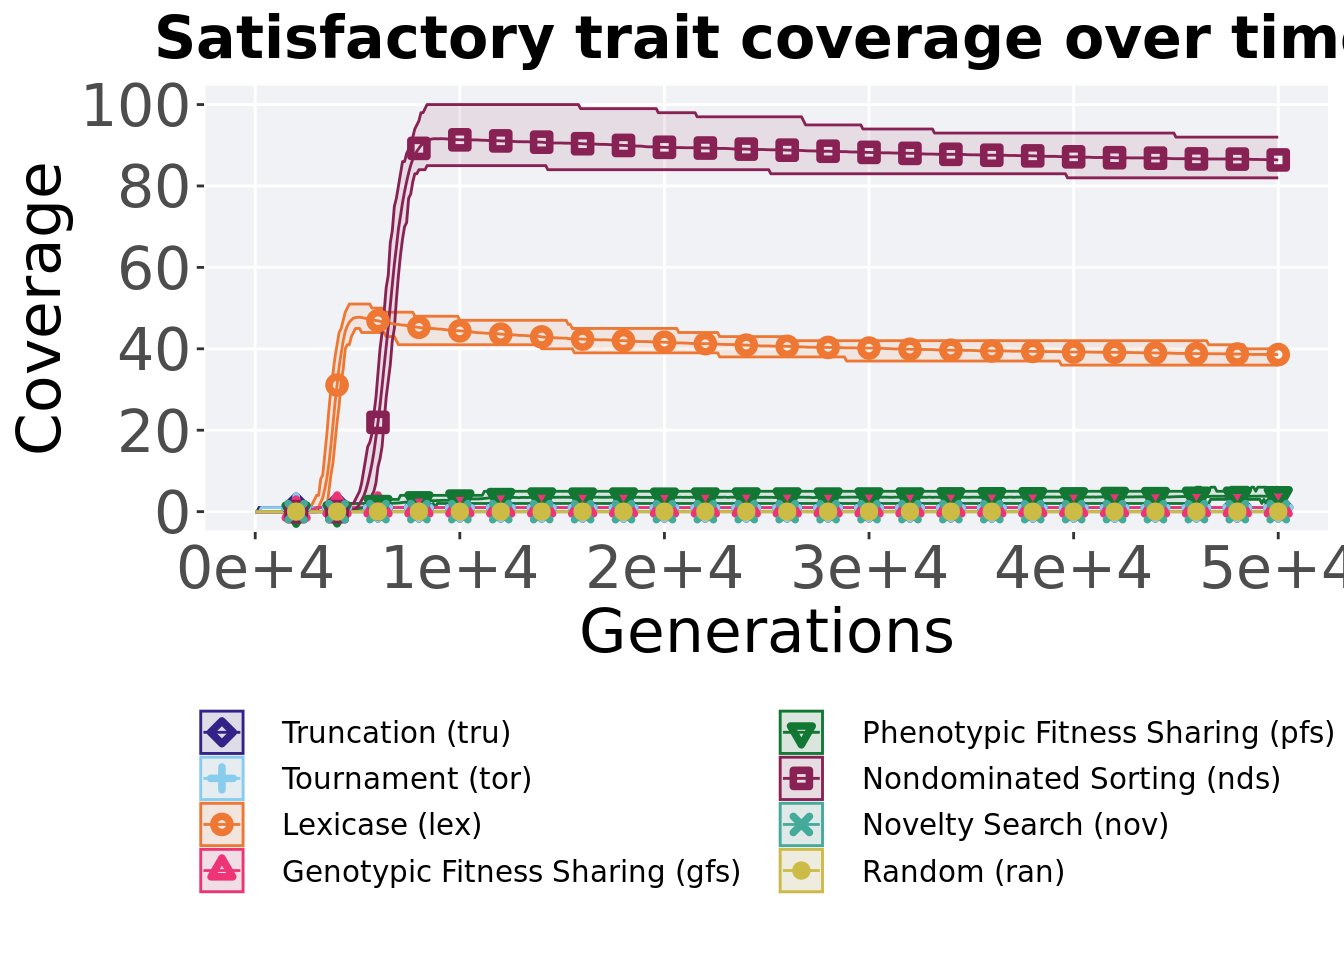
\includegraphics{demo_files/figure-latex/con-sat-ot-1.pdf}

\hypertarget{best-coverage-throughout}{%
\subsection{Best coverage throughout}\label{best-coverage-throughout}}

Best satisfactory trait coverage throughout 50,000 generations.

\begin{Shaded}
\begin{Highlighting}[]
\CommentTok{### best satisfactory trait coverage throughout}
\KeywordTok{filter}\NormalTok{(cc_best, col }\OperatorTok{==}\StringTok{ 'pop_uni_obj'} \OperatorTok{&}\StringTok{ }\NormalTok{diagnostic }\OperatorTok{==}\StringTok{ 'contradictory_objectives'}\NormalTok{) }\OperatorTok
\StringTok{  }\KeywordTok{ggplot}\NormalTok{(., }\KeywordTok{aes}\NormalTok{(}\DataTypeTok{x =}\NormalTok{ acron, }\DataTypeTok{y =}\NormalTok{ val, }\DataTypeTok{color =}\NormalTok{ acron, }\DataTypeTok{fill =}\NormalTok{ acron, }\DataTypeTok{shape =}\NormalTok{ acron)) }\OperatorTok{+}
\StringTok{  }\KeywordTok{geom_flat_violin}\NormalTok{(}\DataTypeTok{position =} \KeywordTok{position_nudge}\NormalTok{(}\DataTypeTok{x =} \FloatTok{.2}\NormalTok{, }\DataTypeTok{y =} \DecValTok{0}\NormalTok{), }\DataTypeTok{scale =} \StringTok{'width'}\NormalTok{, }\DataTypeTok{alpha =} \FloatTok{0.2}\NormalTok{) }\OperatorTok{+}
\StringTok{  }\KeywordTok{geom_point}\NormalTok{(}\DataTypeTok{position =} \KeywordTok{position_jitter}\NormalTok{(}\DataTypeTok{width =} \FloatTok{.1}\NormalTok{), }\DataTypeTok{size =} \FloatTok{1.5}\NormalTok{, }\DataTypeTok{alpha =} \FloatTok{1.0}\NormalTok{) }\OperatorTok{+}
\StringTok{  }\KeywordTok{geom_boxplot}\NormalTok{(}\DataTypeTok{color =} \StringTok{'black'}\NormalTok{, }\DataTypeTok{width =} \FloatTok{.2}\NormalTok{, }\DataTypeTok{outlier.shape =} \OtherTok{NA}\NormalTok{, }\DataTypeTok{alpha =} \FloatTok{0.0}\NormalTok{) }\OperatorTok{+}
\StringTok{  }\KeywordTok{scale_y_continuous}\NormalTok{(}
    \DataTypeTok{name=}\StringTok{"Coverage"}\NormalTok{,}
    \DataTypeTok{limits=}\KeywordTok{c}\NormalTok{(}\DecValTok{0}\NormalTok{, }\DecValTok{100}\NormalTok{),}
    \DataTypeTok{breaks=}\KeywordTok{seq}\NormalTok{(}\DecValTok{0}\NormalTok{,}\DecValTok{100}\NormalTok{, }\DecValTok{20}\NormalTok{),}
    \DataTypeTok{labels=}\KeywordTok{c}\NormalTok{(}\StringTok{"0"}\NormalTok{, }\StringTok{"20"}\NormalTok{, }\StringTok{"40"}\NormalTok{, }\StringTok{"60"}\NormalTok{, }\StringTok{"80"}\NormalTok{, }\StringTok{"100"}\NormalTok{)}
\NormalTok{  ) }\OperatorTok{+}
\StringTok{  }\KeywordTok{scale_x_discrete}\NormalTok{(}
    \DataTypeTok{name=}\StringTok{"Scheme"}
\NormalTok{  )}\OperatorTok{+}
\StringTok{  }\KeywordTok{scale_shape_manual}\NormalTok{(}\DataTypeTok{values=}\NormalTok{SHAPE)}\OperatorTok{+}
\StringTok{  }\KeywordTok{scale_colour_manual}\NormalTok{(}\DataTypeTok{values =}\NormalTok{ cb_palette, ) }\OperatorTok{+}
\StringTok{  }\KeywordTok{scale_fill_manual}\NormalTok{(}\DataTypeTok{values =}\NormalTok{ cb_palette) }\OperatorTok{+}
\StringTok{  }\KeywordTok{ggtitle}\NormalTok{(}\StringTok{'Best satisfactory trait coverage'}\NormalTok{)}\OperatorTok{+}
\StringTok{  }\NormalTok{p_theme }\OperatorTok{+}\StringTok{ }\KeywordTok{theme}\NormalTok{(}\DataTypeTok{legend.title=}\KeywordTok{element_blank}\NormalTok{()) }\OperatorTok{+}
\StringTok{  }\KeywordTok{guides}\NormalTok{(}
    \DataTypeTok{shape=}\KeywordTok{guide_legend}\NormalTok{(}\DataTypeTok{nrow=}\DecValTok{2}\NormalTok{, }\DataTypeTok{title.position =} \StringTok{"bottom"}\NormalTok{),}
    \DataTypeTok{color=}\KeywordTok{guide_legend}\NormalTok{(}\DataTypeTok{nrow=}\DecValTok{2}\NormalTok{, }\DataTypeTok{title.position =} \StringTok{"bottom"}\NormalTok{),}
    \DataTypeTok{fill=}\KeywordTok{guide_legend}\NormalTok{(}\DataTypeTok{nrow=}\DecValTok{2}\NormalTok{, }\DataTypeTok{title.position =} \StringTok{"bottom"}\NormalTok{)}
\NormalTok{  )}
\end{Highlighting}
\end{Shaded}

\begin{verbatim}
## Warning: Removed 60 rows containing missing values (`geom_point()`).
\end{verbatim}

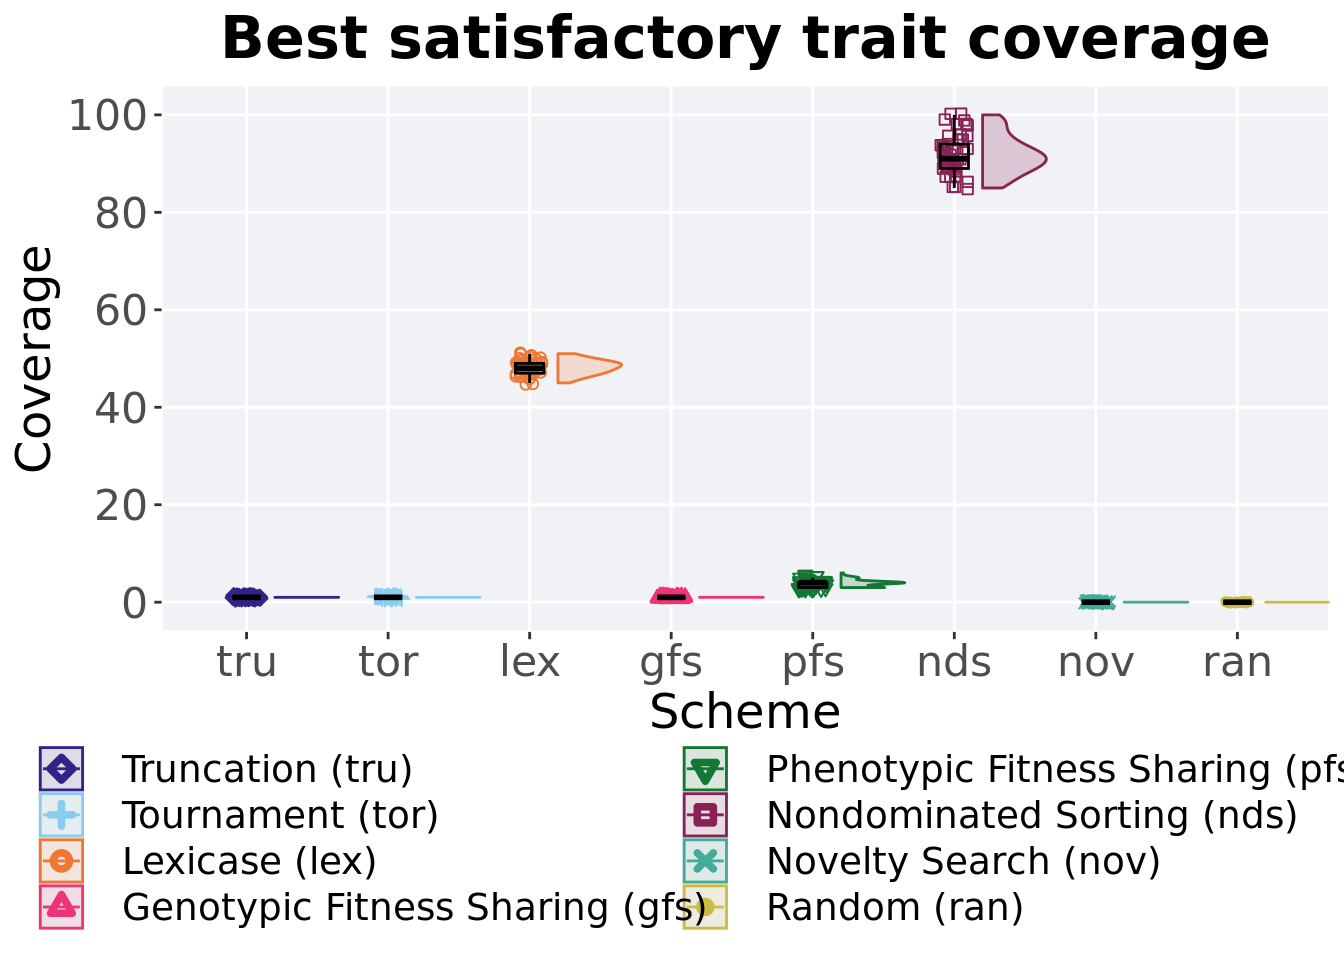
\includegraphics{demo_files/figure-latex/con-sat-bst-1.pdf}

\hypertarget{stats-8}{%
\subsubsection{Stats}\label{stats-8}}

Summary statistics for the best satisfactory trait coverage.

\begin{Shaded}
\begin{Highlighting}[]
\CommentTok{### best}
\NormalTok{coverage =}\StringTok{ }\KeywordTok{filter}\NormalTok{(cc_best, col }\OperatorTok{==}\StringTok{ 'pop_uni_obj'} \OperatorTok{&}\StringTok{ }\NormalTok{diagnostic }\OperatorTok{==}\StringTok{ 'contradictory_objectives'}\NormalTok{)}
\NormalTok{coverage}\OperatorTok{$}\NormalTok{acron =}\StringTok{ }\KeywordTok{factor}\NormalTok{(coverage}\OperatorTok{$}\NormalTok{acron, }\DataTypeTok{levels =} \KeywordTok{c}\NormalTok{(}\StringTok{'nds'}\NormalTok{, }\StringTok{'lex'}\NormalTok{, }\StringTok{'pfs'}\NormalTok{, }\StringTok{'gfs'}\NormalTok{, }\StringTok{'tor'}\NormalTok{, }\StringTok{'tru'}\NormalTok{, }\StringTok{'nov'}\NormalTok{, }\StringTok{'ran'}\NormalTok{))}
\NormalTok{coverage }\OperatorTok
\StringTok{  }\KeywordTok{group_by}\NormalTok{(acron) }\OperatorTok
\StringTok{  }\NormalTok{dplyr}\OperatorTok{::}\KeywordTok{summarise}\NormalTok{(}
    \DataTypeTok{count =} \KeywordTok{n}\NormalTok{(),}
    \DataTypeTok{na_cnt =} \KeywordTok{sum}\NormalTok{(}\KeywordTok{is.na}\NormalTok{(val)),}
    \DataTypeTok{min =} \KeywordTok{min}\NormalTok{(val, }\DataTypeTok{na.rm =} \OtherTok{TRUE}\NormalTok{),}
    \DataTypeTok{median =} \KeywordTok{median}\NormalTok{(val, }\DataTypeTok{na.rm =} \OtherTok{TRUE}\NormalTok{),}
    \DataTypeTok{mean =} \KeywordTok{mean}\NormalTok{(val, }\DataTypeTok{na.rm =} \OtherTok{TRUE}\NormalTok{),}
    \DataTypeTok{max =} \KeywordTok{max}\NormalTok{(val, }\DataTypeTok{na.rm =} \OtherTok{TRUE}\NormalTok{),}
    \DataTypeTok{IQR =} \KeywordTok{IQR}\NormalTok{(val, }\DataTypeTok{na.rm =} \OtherTok{TRUE}\NormalTok{)}
\NormalTok{  )}
\end{Highlighting}
\end{Shaded}

\begin{verbatim}
## # A tibble: 8 x 8
##   acron count na_cnt   min median  mean   max   IQR
##   <fct> <int>  <int> <dbl>  <dbl> <dbl> <dbl> <dbl>
## 1 nds      50      0    85     91 91.8    100     5
## 2 lex      50      0    45     48 48.2     51     2
## 3 pfs      50      0     3      4  3.84     6     1
## 4 gfs      50      0     1      1  1        1     0
## 5 tor      50      0     1      1  1        1     0
## 6 tru      50      0     1      1  1        1     0
## 7 nov      50      0     0      0  0        0     0
## 8 ran      50      0     0      0  0        0     0
\end{verbatim}

Kruskal--Wallis test provides evidence of difference among satisfactory trait coverage.

\begin{Shaded}
\begin{Highlighting}[]
\KeywordTok{kruskal.test}\NormalTok{(val }\OperatorTok{~}\StringTok{ }\NormalTok{acron, }\DataTypeTok{data =}\NormalTok{ coverage)}
\end{Highlighting}
\end{Shaded}

\begin{verbatim}
## 
##  Kruskal-Wallis rank sum test
## 
## data:  val by acron
## Kruskal-Wallis chi-squared = 396.67, df = 7, p-value < 2.2e-16
\end{verbatim}

Results for post-hoc Wilcoxon rank-sum test with a Bonferroni correction on satisfactory trait coverage.

\begin{Shaded}
\begin{Highlighting}[]
\KeywordTok{pairwise.wilcox.test}\NormalTok{(}\DataTypeTok{x =}\NormalTok{ coverage}\OperatorTok{$}\NormalTok{val, }\DataTypeTok{g =}\NormalTok{ coverage}\OperatorTok{$}\NormalTok{acron, }\DataTypeTok{p.adjust.method =} \StringTok{"bonferroni"}\NormalTok{,}
                     \DataTypeTok{paired =} \OtherTok{FALSE}\NormalTok{, }\DataTypeTok{conf.int =} \OtherTok{FALSE}\NormalTok{, }\DataTypeTok{alternative =} \StringTok{'l'}\NormalTok{)}
\end{Highlighting}
\end{Shaded}

\begin{verbatim}
## 
##  Pairwise comparisons using Wilcoxon rank sum test with continuity correction 
## 
## data:  coverage$val and coverage$acron 
## 
##     nds    lex    pfs    gfs    tor    tru    nov
## lex <2e-16 -      -      -      -      -      -  
## pfs <2e-16 <2e-16 -      -      -      -      -  
## gfs <2e-16 <2e-16 <2e-16 -      -      -      -  
## tor <2e-16 <2e-16 <2e-16 1      -      -      -  
## tru <2e-16 <2e-16 <2e-16 1      1      -      -  
## nov <2e-16 <2e-16 <2e-16 <2e-16 <2e-16 <2e-16 -  
## ran <2e-16 <2e-16 <2e-16 <2e-16 <2e-16 <2e-16 1  
## 
## P value adjustment method: bonferroni
\end{verbatim}

\hypertarget{end-of-50000-generations}{%
\subsection{End of 50,000 generations}\label{end-of-50000-generations}}

Satisfactory trait coverage in the population at the end of 50,000 generations.

\begin{Shaded}
\begin{Highlighting}[]
\CommentTok{### end of run}
\KeywordTok{filter}\NormalTok{(cc_over_time, diagnostic }\OperatorTok{==}\StringTok{ 'contradictory_objectives'} \OperatorTok{&}\StringTok{ }\NormalTok{gen }\OperatorTok{==}\StringTok{ }\DecValTok{50000}\NormalTok{) }\OperatorTok
\StringTok{  }\KeywordTok{ggplot}\NormalTok{(., }\KeywordTok{aes}\NormalTok{(}\DataTypeTok{x =}\NormalTok{ acron, }\DataTypeTok{y =}\NormalTok{ pop_uni_obj, }\DataTypeTok{color =}\NormalTok{ acron, }\DataTypeTok{fill =}\NormalTok{ acron, }\DataTypeTok{shape =}\NormalTok{ acron)) }\OperatorTok{+}
\StringTok{  }\KeywordTok{geom_flat_violin}\NormalTok{(}\DataTypeTok{position =} \KeywordTok{position_nudge}\NormalTok{(}\DataTypeTok{x =} \FloatTok{.2}\NormalTok{, }\DataTypeTok{y =} \DecValTok{0}\NormalTok{), }\DataTypeTok{scale =} \StringTok{'width'}\NormalTok{, }\DataTypeTok{alpha =} \FloatTok{0.2}\NormalTok{) }\OperatorTok{+}
\StringTok{  }\KeywordTok{geom_point}\NormalTok{(}\DataTypeTok{position =} \KeywordTok{position_jitter}\NormalTok{(}\DataTypeTok{width =} \FloatTok{.1}\NormalTok{), }\DataTypeTok{size =} \FloatTok{1.5}\NormalTok{, }\DataTypeTok{alpha =} \FloatTok{1.0}\NormalTok{) }\OperatorTok{+}
\StringTok{  }\KeywordTok{geom_boxplot}\NormalTok{(}\DataTypeTok{color =} \StringTok{'black'}\NormalTok{, }\DataTypeTok{width =} \FloatTok{.2}\NormalTok{, }\DataTypeTok{outlier.shape =} \OtherTok{NA}\NormalTok{, }\DataTypeTok{alpha =} \FloatTok{0.0}\NormalTok{) }\OperatorTok{+}
\StringTok{  }\KeywordTok{scale_y_continuous}\NormalTok{(}
    \DataTypeTok{name=}\StringTok{"Coverage"}\NormalTok{,}
    \DataTypeTok{limits=}\KeywordTok{c}\NormalTok{(}\DecValTok{0}\NormalTok{, }\DecValTok{100}\NormalTok{),}
    \DataTypeTok{breaks=}\KeywordTok{seq}\NormalTok{(}\DecValTok{0}\NormalTok{,}\DecValTok{100}\NormalTok{, }\DecValTok{20}\NormalTok{),}
    \DataTypeTok{labels=}\KeywordTok{c}\NormalTok{(}\StringTok{"0"}\NormalTok{, }\StringTok{"20"}\NormalTok{, }\StringTok{"40"}\NormalTok{, }\StringTok{"60"}\NormalTok{, }\StringTok{"80"}\NormalTok{, }\StringTok{"100"}\NormalTok{)}
\NormalTok{  ) }\OperatorTok{+}
\StringTok{  }\KeywordTok{scale_x_discrete}\NormalTok{(}
    \DataTypeTok{name=}\StringTok{"Scheme"}
\NormalTok{  )}\OperatorTok{+}
\StringTok{  }\KeywordTok{scale_shape_manual}\NormalTok{(}\DataTypeTok{values=}\NormalTok{SHAPE)}\OperatorTok{+}
\StringTok{  }\KeywordTok{scale_colour_manual}\NormalTok{(}\DataTypeTok{values =}\NormalTok{ cb_palette, ) }\OperatorTok{+}
\StringTok{  }\KeywordTok{scale_fill_manual}\NormalTok{(}\DataTypeTok{values =}\NormalTok{ cb_palette) }\OperatorTok{+}
\StringTok{  }\KeywordTok{ggtitle}\NormalTok{(}\StringTok{'Final satisfactory trait coverage'}\NormalTok{)}\OperatorTok{+}
\StringTok{  }\NormalTok{p_theme }\OperatorTok{+}\StringTok{ }\KeywordTok{theme}\NormalTok{(}\DataTypeTok{legend.title=}\KeywordTok{element_blank}\NormalTok{()) }\OperatorTok{+}
\StringTok{  }\KeywordTok{guides}\NormalTok{(}
    \DataTypeTok{shape=}\KeywordTok{guide_legend}\NormalTok{(}\DataTypeTok{nrow=}\DecValTok{2}\NormalTok{, }\DataTypeTok{title.position =} \StringTok{"bottom"}\NormalTok{),}
    \DataTypeTok{color=}\KeywordTok{guide_legend}\NormalTok{(}\DataTypeTok{nrow=}\DecValTok{2}\NormalTok{, }\DataTypeTok{title.position =} \StringTok{"bottom"}\NormalTok{),}
    \DataTypeTok{fill=}\KeywordTok{guide_legend}\NormalTok{(}\DataTypeTok{nrow=}\DecValTok{2}\NormalTok{, }\DataTypeTok{title.position =} \StringTok{"bottom"}\NormalTok{)}
\NormalTok{  )}
\end{Highlighting}
\end{Shaded}

\begin{verbatim}
## Warning: Removed 56 rows containing missing values (`geom_point()`).
\end{verbatim}

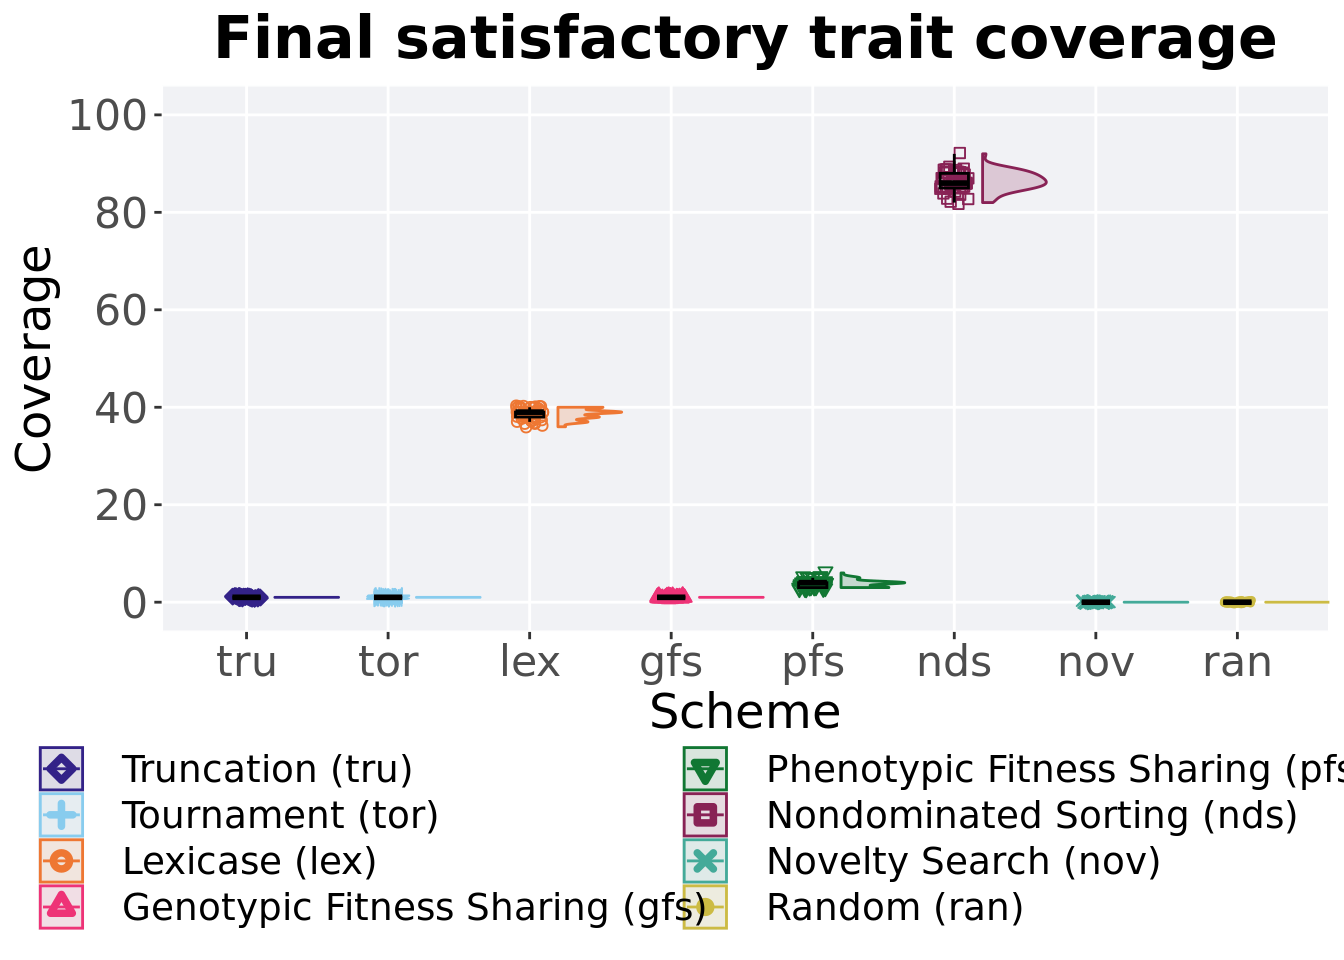
\includegraphics{demo_files/figure-latex/con-sat-end-1.pdf}

\hypertarget{stats-9}{%
\subsubsection{Stats}\label{stats-9}}

Summary statistics for satisfactory trait coverage in the population at the end of 50,000 generations.

\begin{Shaded}
\begin{Highlighting}[]
\CommentTok{### end of run}
\NormalTok{coverage =}\StringTok{ }\KeywordTok{filter}\NormalTok{(cc_over_time, diagnostic }\OperatorTok{==}\StringTok{ 'contradictory_objectives'} \OperatorTok{&}\StringTok{ }\NormalTok{gen }\OperatorTok{==}\StringTok{ }\DecValTok{50000}\NormalTok{)}
\NormalTok{coverage}\OperatorTok{$}\NormalTok{acron =}\StringTok{ }\KeywordTok{factor}\NormalTok{(coverage}\OperatorTok{$}\NormalTok{acron, }\DataTypeTok{levels =} \KeywordTok{c}\NormalTok{(}\StringTok{'nds'}\NormalTok{, }\StringTok{'lex'}\NormalTok{, }\StringTok{'pfs'}\NormalTok{, }\StringTok{'gfs'}\NormalTok{, }\StringTok{'tor'}\NormalTok{, }\StringTok{'tru'}\NormalTok{, }\StringTok{'nov'}\NormalTok{, }\StringTok{'ran'}\NormalTok{))}
\NormalTok{coverage }\OperatorTok
\StringTok{  }\KeywordTok{group_by}\NormalTok{(acron) }\OperatorTok
\StringTok{  }\NormalTok{dplyr}\OperatorTok{::}\KeywordTok{summarise}\NormalTok{(}
    \DataTypeTok{count =} \KeywordTok{n}\NormalTok{(),}
    \DataTypeTok{na_cnt =} \KeywordTok{sum}\NormalTok{(}\KeywordTok{is.na}\NormalTok{(pop_uni_obj)),}
    \DataTypeTok{min =} \KeywordTok{min}\NormalTok{(pop_uni_obj, }\DataTypeTok{na.rm =} \OtherTok{TRUE}\NormalTok{),}
    \DataTypeTok{median =} \KeywordTok{median}\NormalTok{(pop_uni_obj, }\DataTypeTok{na.rm =} \OtherTok{TRUE}\NormalTok{),}
    \DataTypeTok{mean =} \KeywordTok{mean}\NormalTok{(pop_uni_obj, }\DataTypeTok{na.rm =} \OtherTok{TRUE}\NormalTok{),}
    \DataTypeTok{max =} \KeywordTok{max}\NormalTok{(pop_uni_obj, }\DataTypeTok{na.rm =} \OtherTok{TRUE}\NormalTok{),}
    \DataTypeTok{IQR =} \KeywordTok{IQR}\NormalTok{(pop_uni_obj, }\DataTypeTok{na.rm =} \OtherTok{TRUE}\NormalTok{)}
\NormalTok{  )}
\end{Highlighting}
\end{Shaded}

\begin{verbatim}
## # A tibble: 8 x 8
##   acron count na_cnt   min median  mean   max   IQR
##   <fct> <int>  <int> <int>  <dbl> <dbl> <int> <dbl>
## 1 nds      50      0    82     86 86.4     92     3
## 2 lex      50      0    36     39 38.6     40     1
## 3 pfs      50      0     3      4  3.82     6     1
## 4 gfs      50      0     1      1  1        1     0
## 5 tor      50      0     1      1  1        1     0
## 6 tru      50      0     1      1  1        1     0
## 7 nov      50      0     0      0  0        0     0
## 8 ran      50      0     0      0  0        0     0
\end{verbatim}

Kruskal--Wallis test provides evidence of difference among satisfactory trait coverage in the population at the end of 50,000 generations.

\begin{Shaded}
\begin{Highlighting}[]
\KeywordTok{kruskal.test}\NormalTok{(pop_uni_obj }\OperatorTok{~}\StringTok{ }\NormalTok{acron, }\DataTypeTok{data =}\NormalTok{ coverage)}
\end{Highlighting}
\end{Shaded}

\begin{verbatim}
## 
##  Kruskal-Wallis rank sum test
## 
## data:  pop_uni_obj by acron
## Kruskal-Wallis chi-squared = 396.7, df = 7, p-value < 2.2e-16
\end{verbatim}

Results for post-hoc Wilcoxon rank-sum test with a Bonferroni correction on satisfactory trait coverage in the population at the end of 50,000 generations.

\begin{Shaded}
\begin{Highlighting}[]
\KeywordTok{pairwise.wilcox.test}\NormalTok{(}\DataTypeTok{x =}\NormalTok{ coverage}\OperatorTok{$}\NormalTok{pop_uni_obj, }\DataTypeTok{g =}\NormalTok{ coverage}\OperatorTok{$}\NormalTok{acron, }\DataTypeTok{p.adjust.method =} \StringTok{"bonferroni"}\NormalTok{,}
                     \DataTypeTok{paired =} \OtherTok{FALSE}\NormalTok{, }\DataTypeTok{conf.int =} \OtherTok{FALSE}\NormalTok{, }\DataTypeTok{alternative =} \StringTok{'l'}\NormalTok{)}
\end{Highlighting}
\end{Shaded}

\begin{verbatim}
## 
##  Pairwise comparisons using Wilcoxon rank sum test with continuity correction 
## 
## data:  coverage$pop_uni_obj and coverage$acron 
## 
##     nds    lex    pfs    gfs    tor    tru    nov
## lex <2e-16 -      -      -      -      -      -  
## pfs <2e-16 <2e-16 -      -      -      -      -  
## gfs <2e-16 <2e-16 <2e-16 -      -      -      -  
## tor <2e-16 <2e-16 <2e-16 1      -      -      -  
## tru <2e-16 <2e-16 <2e-16 1      1      -      -  
## nov <2e-16 <2e-16 <2e-16 <2e-16 <2e-16 <2e-16 -  
## ran <2e-16 <2e-16 <2e-16 <2e-16 <2e-16 <2e-16 1  
## 
## P value adjustment method: bonferroni
\end{verbatim}

\hypertarget{activation-gene-coverage}{%
\section{Activation gene coverage}\label{activation-gene-coverage}}

Activation gene coverage analysis.

\hypertarget{over-time-coverage}{%
\subsection{Over time coverage}\label{over-time-coverage}}

Activation gene coverage over time.

\begin{Shaded}
\begin{Highlighting}[]
\CommentTok{# data for lines and shading on plots}
\NormalTok{lines =}\StringTok{ }\KeywordTok{filter}\NormalTok{(cc_over_time, diagnostic }\OperatorTok{==}\StringTok{ 'contradictory_objectives'}\NormalTok{) }\OperatorTok
\StringTok{  }\KeywordTok{group_by}\NormalTok{(}\StringTok{`}\DataTypeTok{Selection}\CharTok{\textbackslash{}n}\DataTypeTok{Scheme}\StringTok{`}\NormalTok{, gen) }\OperatorTok
\StringTok{  }\NormalTok{dplyr}\OperatorTok{::}\KeywordTok{summarise}\NormalTok{(}
    \DataTypeTok{min =} \KeywordTok{min}\NormalTok{(uni_str_pos),}
    \DataTypeTok{mean =} \KeywordTok{mean}\NormalTok{(uni_str_pos),}
    \DataTypeTok{max =} \KeywordTok{max}\NormalTok{(uni_str_pos)}
\NormalTok{  )}
\end{Highlighting}
\end{Shaded}

\begin{verbatim}
## `summarise()` has grouped output by 'Selection Scheme'. You can override using
## the `.groups` argument.
\end{verbatim}

\begin{Shaded}
\begin{Highlighting}[]
\KeywordTok{ggplot}\NormalTok{(lines, }\KeywordTok{aes}\NormalTok{(}\DataTypeTok{x=}\NormalTok{gen, }\DataTypeTok{y=}\NormalTok{mean, }\DataTypeTok{group =} \StringTok{`}\DataTypeTok{Selection}\CharTok{\textbackslash{}n}\DataTypeTok{Scheme}\StringTok{`}\NormalTok{, }\DataTypeTok{fill =}\StringTok{`}\DataTypeTok{Selection}\CharTok{\textbackslash{}n}\DataTypeTok{Scheme}\StringTok{`}\NormalTok{, }\DataTypeTok{color =} \StringTok{`}\DataTypeTok{Selection}\CharTok{\textbackslash{}n}\DataTypeTok{Scheme}\StringTok{`}\NormalTok{, }\DataTypeTok{shape =} \StringTok{`}\DataTypeTok{Selection}\CharTok{\textbackslash{}n}\DataTypeTok{Scheme}\StringTok{`}\NormalTok{)) }\OperatorTok{+}
\StringTok{  }\KeywordTok{geom_ribbon}\NormalTok{(}\KeywordTok{aes}\NormalTok{(}\DataTypeTok{ymin =}\NormalTok{ min, }\DataTypeTok{ymax =}\NormalTok{ max), }\DataTypeTok{alpha =} \FloatTok{0.1}\NormalTok{) }\OperatorTok{+}
\StringTok{  }\KeywordTok{geom_line}\NormalTok{(}\DataTypeTok{size =} \FloatTok{0.5}\NormalTok{) }\OperatorTok{+}
\StringTok{  }\KeywordTok{geom_point}\NormalTok{(}\DataTypeTok{data =} \KeywordTok{filter}\NormalTok{(lines, gen }\OperatorTok\StringTok{ }\DecValTok{2000} \OperatorTok{==}\StringTok{ }\DecValTok{0} \OperatorTok{&}\StringTok{ }\NormalTok{gen }\OperatorTok{!=}\StringTok{ }\DecValTok{0}\NormalTok{), }\DataTypeTok{size =} \FloatTok{1.5}\NormalTok{, }\DataTypeTok{stroke =} \FloatTok{2.0}\NormalTok{, }\DataTypeTok{alpha =} \FloatTok{1.0}\NormalTok{) }\OperatorTok{+}
\StringTok{  }\KeywordTok{scale_y_continuous}\NormalTok{(}
    \DataTypeTok{name=}\StringTok{"Coverage"}\NormalTok{,}
    \DataTypeTok{limits=}\KeywordTok{c}\NormalTok{(}\DecValTok{0}\NormalTok{, }\DecValTok{100}\NormalTok{),}
    \DataTypeTok{breaks=}\KeywordTok{seq}\NormalTok{(}\DecValTok{0}\NormalTok{,}\DecValTok{100}\NormalTok{, }\DecValTok{20}\NormalTok{),}
    \DataTypeTok{labels=}\KeywordTok{c}\NormalTok{(}\StringTok{"0"}\NormalTok{, }\StringTok{"20"}\NormalTok{, }\StringTok{"40"}\NormalTok{, }\StringTok{"60"}\NormalTok{, }\StringTok{"80"}\NormalTok{, }\StringTok{"100"}\NormalTok{)}
\NormalTok{  ) }\OperatorTok{+}
\StringTok{  }\KeywordTok{scale_x_continuous}\NormalTok{(}
    \DataTypeTok{name=}\StringTok{"Generations"}\NormalTok{,}
    \DataTypeTok{limits=}\KeywordTok{c}\NormalTok{(}\DecValTok{0}\NormalTok{, }\DecValTok{50000}\NormalTok{),}
    \DataTypeTok{breaks=}\KeywordTok{c}\NormalTok{(}\DecValTok{0}\NormalTok{, }\DecValTok{10000}\NormalTok{, }\DecValTok{20000}\NormalTok{, }\DecValTok{30000}\NormalTok{, }\DecValTok{40000}\NormalTok{, }\DecValTok{50000}\NormalTok{),}
    \DataTypeTok{labels=}\KeywordTok{c}\NormalTok{(}\StringTok{"0e+4"}\NormalTok{, }\StringTok{"1e+4"}\NormalTok{, }\StringTok{"2e+4"}\NormalTok{, }\StringTok{"3e+4"}\NormalTok{, }\StringTok{"4e+4"}\NormalTok{, }\StringTok{"5e+4"}\NormalTok{)}
\NormalTok{  ) }\OperatorTok{+}
\StringTok{  }\KeywordTok{scale_shape_manual}\NormalTok{(}\DataTypeTok{values=}\NormalTok{SHAPE)}\OperatorTok{+}
\StringTok{  }\KeywordTok{scale_colour_manual}\NormalTok{(}\DataTypeTok{values =}\NormalTok{ cb_palette) }\OperatorTok{+}
\StringTok{  }\KeywordTok{scale_fill_manual}\NormalTok{(}\DataTypeTok{values =}\NormalTok{ cb_palette) }\OperatorTok{+}
\StringTok{  }\KeywordTok{ggtitle}\NormalTok{(}\StringTok{'Activation gene coverage over time'}\NormalTok{)}\OperatorTok{+}
\StringTok{  }\NormalTok{p_theme }\OperatorTok{+}\StringTok{ }\KeywordTok{theme}\NormalTok{(}\DataTypeTok{legend.title=}\KeywordTok{element_blank}\NormalTok{(),}\DataTypeTok{legend.text=}\KeywordTok{element_text}\NormalTok{(}\DataTypeTok{size=}\DecValTok{11}\NormalTok{)) }\OperatorTok{+}
\StringTok{  }\KeywordTok{guides}\NormalTok{(}
    \DataTypeTok{shape=}\KeywordTok{guide_legend}\NormalTok{(}\DataTypeTok{ncol=}\DecValTok{2}\NormalTok{, }\DataTypeTok{title.position =} \StringTok{"bottom"}\NormalTok{),}
    \DataTypeTok{color=}\KeywordTok{guide_legend}\NormalTok{(}\DataTypeTok{ncol=}\DecValTok{2}\NormalTok{, }\DataTypeTok{title.position =} \StringTok{"bottom"}\NormalTok{),}
    \DataTypeTok{fill=}\KeywordTok{guide_legend}\NormalTok{(}\DataTypeTok{ncol=}\DecValTok{2}\NormalTok{, }\DataTypeTok{title.position =} \StringTok{"bottom"}\NormalTok{)}
\NormalTok{  )}
\end{Highlighting}
\end{Shaded}

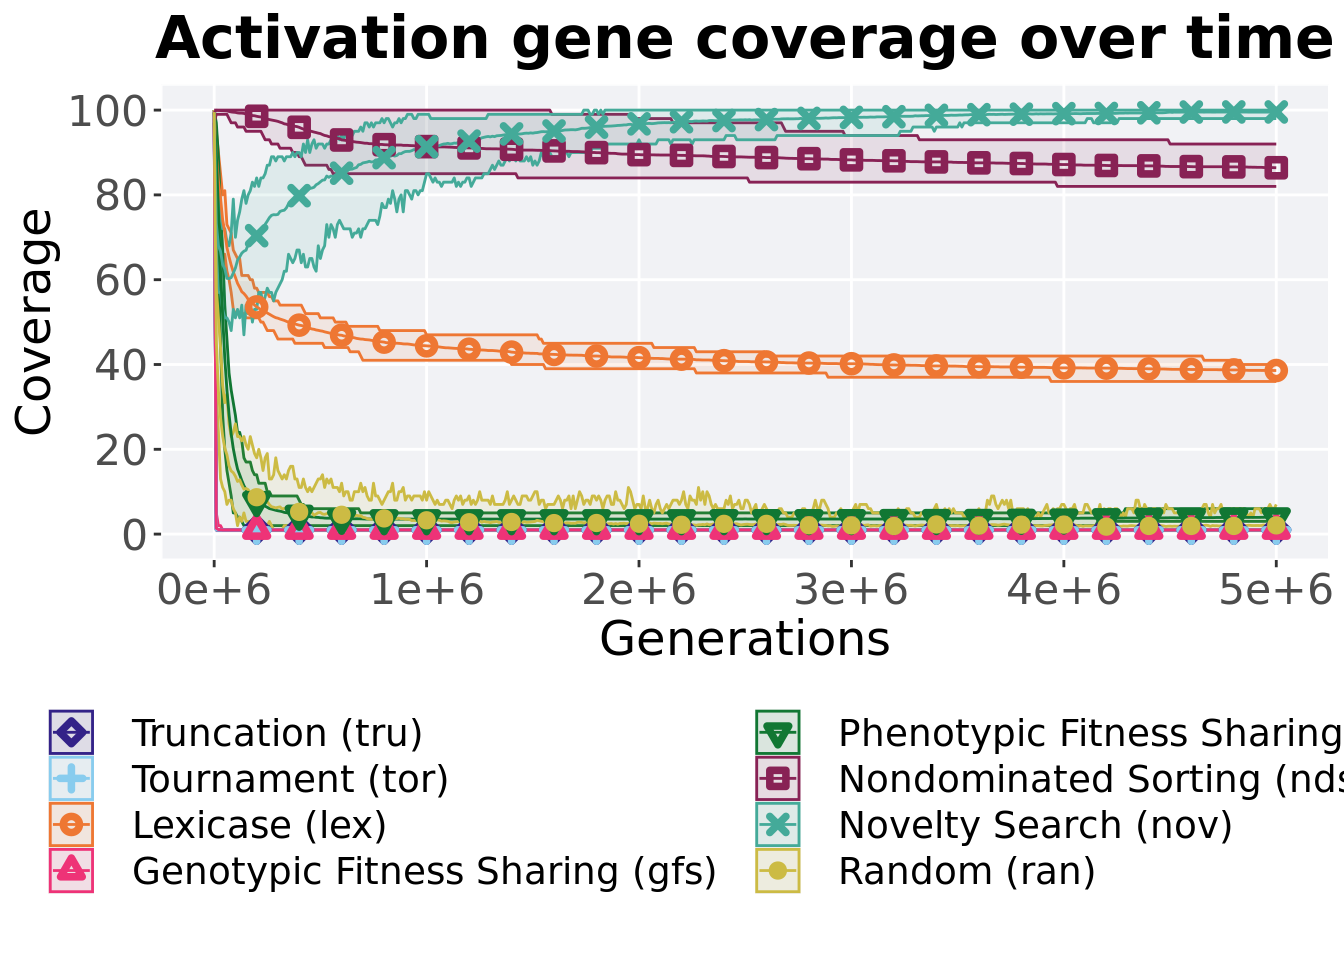
\includegraphics{demo_files/figure-latex/con-act-ot-1.pdf}

\hypertarget{end-of-50000-generations-1}{%
\subsection{End of 50,000 generations}\label{end-of-50000-generations-1}}

Activation gene coverage in the population at the end of 50,000 generations.

\begin{Shaded}
\begin{Highlighting}[]
\CommentTok{# end of run}
\KeywordTok{filter}\NormalTok{(cc_over_time, diagnostic }\OperatorTok{==}\StringTok{ 'contradictory_objectives'} \OperatorTok{&}\StringTok{ }\NormalTok{gen }\OperatorTok{==}\StringTok{ }\DecValTok{50000}\NormalTok{) }\OperatorTok
\StringTok{  }\KeywordTok{ggplot}\NormalTok{(., }\KeywordTok{aes}\NormalTok{(}\DataTypeTok{x =}\NormalTok{ acron, }\DataTypeTok{y =}\NormalTok{ uni_str_pos, }\DataTypeTok{color =}\NormalTok{ acron, }\DataTypeTok{fill =}\NormalTok{ acron, }\DataTypeTok{shape =}\NormalTok{ acron)) }\OperatorTok{+}
\StringTok{  }\KeywordTok{geom_flat_violin}\NormalTok{(}\DataTypeTok{position =} \KeywordTok{position_nudge}\NormalTok{(}\DataTypeTok{x =} \FloatTok{.2}\NormalTok{, }\DataTypeTok{y =} \DecValTok{0}\NormalTok{), }\DataTypeTok{scale =} \StringTok{'width'}\NormalTok{, }\DataTypeTok{alpha =} \FloatTok{0.2}\NormalTok{) }\OperatorTok{+}
\StringTok{  }\KeywordTok{geom_point}\NormalTok{(}\DataTypeTok{position =} \KeywordTok{position_jitter}\NormalTok{(}\DataTypeTok{width =} \FloatTok{.1}\NormalTok{), }\DataTypeTok{size =} \FloatTok{1.5}\NormalTok{, }\DataTypeTok{alpha =} \FloatTok{1.0}\NormalTok{) }\OperatorTok{+}
\StringTok{  }\KeywordTok{geom_boxplot}\NormalTok{(}\DataTypeTok{color =} \StringTok{'black'}\NormalTok{, }\DataTypeTok{width =} \FloatTok{.2}\NormalTok{, }\DataTypeTok{outlier.shape =} \OtherTok{NA}\NormalTok{, }\DataTypeTok{alpha =} \FloatTok{0.0}\NormalTok{) }\OperatorTok{+}
\StringTok{  }\KeywordTok{scale_y_continuous}\NormalTok{(}
    \DataTypeTok{name=}\StringTok{"Coverage"}\NormalTok{,}
    \DataTypeTok{limits=}\KeywordTok{c}\NormalTok{(}\DecValTok{0}\NormalTok{, }\DecValTok{100}\NormalTok{),}
    \DataTypeTok{breaks=}\KeywordTok{seq}\NormalTok{(}\DecValTok{0}\NormalTok{,}\DecValTok{100}\NormalTok{, }\DecValTok{20}\NormalTok{),}
    \DataTypeTok{labels=}\KeywordTok{c}\NormalTok{(}\StringTok{"0"}\NormalTok{, }\StringTok{"20"}\NormalTok{, }\StringTok{"40"}\NormalTok{, }\StringTok{"60"}\NormalTok{, }\StringTok{"80"}\NormalTok{, }\StringTok{"100"}\NormalTok{)}
\NormalTok{  ) }\OperatorTok{+}
\StringTok{  }\KeywordTok{scale_x_discrete}\NormalTok{(}
    \DataTypeTok{name=}\StringTok{"Scheme"}
\NormalTok{  )}\OperatorTok{+}
\StringTok{  }\KeywordTok{scale_shape_manual}\NormalTok{(}\DataTypeTok{values=}\NormalTok{SHAPE)}\OperatorTok{+}
\StringTok{  }\KeywordTok{scale_colour_manual}\NormalTok{(}\DataTypeTok{values =}\NormalTok{ cb_palette, ) }\OperatorTok{+}
\StringTok{  }\KeywordTok{scale_fill_manual}\NormalTok{(}\DataTypeTok{values =}\NormalTok{ cb_palette) }\OperatorTok{+}
\StringTok{  }\KeywordTok{ggtitle}\NormalTok{(}\StringTok{'Final activation gene coverage'}\NormalTok{)}\OperatorTok{+}
\StringTok{  }\NormalTok{p_theme }\OperatorTok{+}\StringTok{ }\KeywordTok{theme}\NormalTok{(}\DataTypeTok{legend.title=}\KeywordTok{element_blank}\NormalTok{()) }\OperatorTok{+}
\StringTok{  }\KeywordTok{guides}\NormalTok{(}
    \DataTypeTok{shape=}\KeywordTok{guide_legend}\NormalTok{(}\DataTypeTok{nrow=}\DecValTok{2}\NormalTok{, }\DataTypeTok{title.position =} \StringTok{"bottom"}\NormalTok{),}
    \DataTypeTok{color=}\KeywordTok{guide_legend}\NormalTok{(}\DataTypeTok{nrow=}\DecValTok{2}\NormalTok{, }\DataTypeTok{title.position =} \StringTok{"bottom"}\NormalTok{),}
    \DataTypeTok{fill=}\KeywordTok{guide_legend}\NormalTok{(}\DataTypeTok{nrow=}\DecValTok{2}\NormalTok{, }\DataTypeTok{title.position =} \StringTok{"bottom"}\NormalTok{)}
\NormalTok{  )}
\end{Highlighting}
\end{Shaded}

\begin{verbatim}
## Warning: Removed 14 rows containing missing values (`geom_point()`).
\end{verbatim}

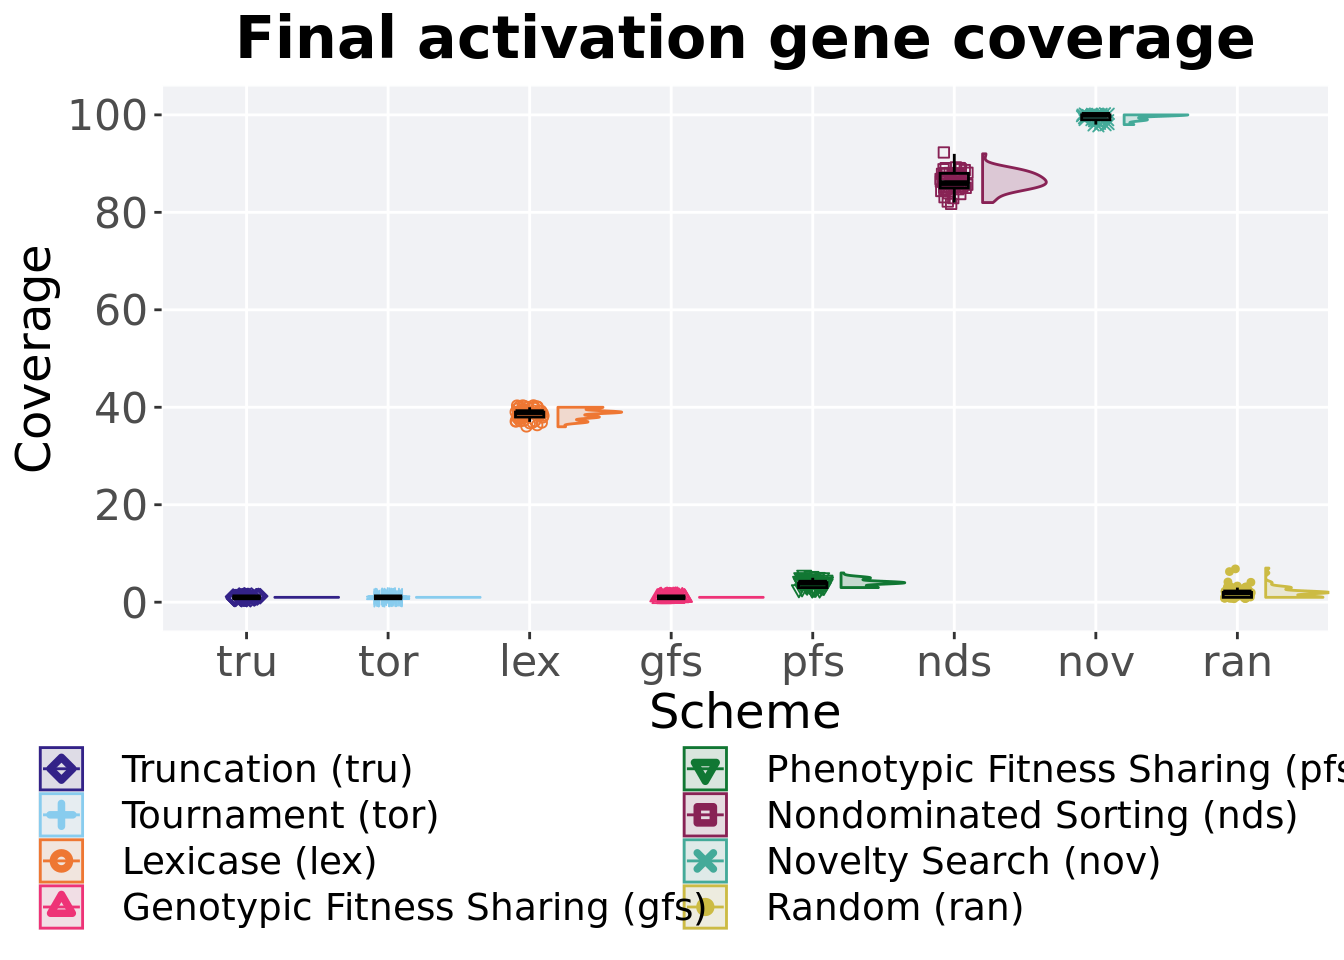
\includegraphics{demo_files/figure-latex/con-act-end-1.pdf}

\hypertarget{stats-10}{%
\subsubsection{Stats}\label{stats-10}}

Summary statistics for activation gene coverage.

\begin{Shaded}
\begin{Highlighting}[]
\CommentTok{# end of run}
\NormalTok{coverage =}\StringTok{ }\KeywordTok{filter}\NormalTok{(cc_over_time, diagnostic }\OperatorTok{==}\StringTok{ 'contradictory_objectives'} \OperatorTok{&}\StringTok{ }\NormalTok{gen }\OperatorTok{==}\StringTok{ }\DecValTok{50000}\NormalTok{)}
\NormalTok{coverage}\OperatorTok{$}\NormalTok{acron =}\StringTok{ }\KeywordTok{factor}\NormalTok{(coverage}\OperatorTok{$}\NormalTok{acron, }\DataTypeTok{levels =} \KeywordTok{c}\NormalTok{(}\StringTok{'nov'}\NormalTok{, }\StringTok{'nds'}\NormalTok{, }\StringTok{'lex'}\NormalTok{, }\StringTok{'pfs'}\NormalTok{, }\StringTok{'ran'}\NormalTok{, }\StringTok{'gfs'}\NormalTok{, }\StringTok{'tor'}\NormalTok{, }\StringTok{'tru'}\NormalTok{))}
\NormalTok{coverage }\OperatorTok
\StringTok{  }\KeywordTok{group_by}\NormalTok{(acron) }\OperatorTok
\StringTok{  }\NormalTok{dplyr}\OperatorTok{::}\KeywordTok{summarise}\NormalTok{(}
    \DataTypeTok{count =} \KeywordTok{n}\NormalTok{(),}
    \DataTypeTok{na_cnt =} \KeywordTok{sum}\NormalTok{(}\KeywordTok{is.na}\NormalTok{(uni_str_pos)),}
    \DataTypeTok{min =} \KeywordTok{min}\NormalTok{(uni_str_pos, }\DataTypeTok{na.rm =} \OtherTok{TRUE}\NormalTok{),}
    \DataTypeTok{median =} \KeywordTok{median}\NormalTok{(uni_str_pos, }\DataTypeTok{na.rm =} \OtherTok{TRUE}\NormalTok{),}
    \DataTypeTok{mean =} \KeywordTok{mean}\NormalTok{(uni_str_pos, }\DataTypeTok{na.rm =} \OtherTok{TRUE}\NormalTok{),}
    \DataTypeTok{max =} \KeywordTok{max}\NormalTok{(uni_str_pos, }\DataTypeTok{na.rm =} \OtherTok{TRUE}\NormalTok{),}
    \DataTypeTok{IQR =} \KeywordTok{IQR}\NormalTok{(uni_str_pos, }\DataTypeTok{na.rm =} \OtherTok{TRUE}\NormalTok{)}
\NormalTok{  )}
\end{Highlighting}
\end{Shaded}

\begin{verbatim}
## # A tibble: 8 x 8
##   acron count na_cnt   min median  mean   max   IQR
##   <fct> <int>  <int> <int>  <dbl> <dbl> <int> <dbl>
## 1 nov      50      0    98    100 99.6    100     1
## 2 nds      50      0    82     86 86.4     92     3
## 3 lex      50      0    36     39 38.6     40     1
## 4 pfs      50      0     3      4  3.98     6     1
## 5 ran      50      0     1      2  2.06     7     1
## 6 gfs      50      0     1      1  1        1     0
## 7 tor      50      0     1      1  1        1     0
## 8 tru      50      0     1      1  1        1     0
\end{verbatim}

Kruskal--Wallis test provides evidence of difference among activation gene coverage.

\begin{Shaded}
\begin{Highlighting}[]
\KeywordTok{kruskal.test}\NormalTok{(uni_str_pos }\OperatorTok{~}\StringTok{ }\NormalTok{acron, }\DataTypeTok{data =}\NormalTok{ coverage)}
\end{Highlighting}
\end{Shaded}

\begin{verbatim}
## 
##  Kruskal-Wallis rank sum test
## 
## data:  uni_str_pos by acron
## Kruskal-Wallis chi-squared = 384.23, df = 7, p-value < 2.2e-16
\end{verbatim}

Results for post-hoc Wilcoxon rank-sum test with a Bonferroni correction on activation gene coverage.

\begin{Shaded}
\begin{Highlighting}[]
\KeywordTok{pairwise.wilcox.test}\NormalTok{(}\DataTypeTok{x =}\NormalTok{ coverage}\OperatorTok{$}\NormalTok{uni_str_pos, }\DataTypeTok{g =}\NormalTok{ coverage}\OperatorTok{$}\NormalTok{acron, }\DataTypeTok{p.adjust.method =} \StringTok{"bonferroni"}\NormalTok{,}
                     \DataTypeTok{paired =} \OtherTok{FALSE}\NormalTok{, }\DataTypeTok{conf.int =} \OtherTok{FALSE}\NormalTok{, }\DataTypeTok{alternative =} \StringTok{'l'}\NormalTok{)}
\end{Highlighting}
\end{Shaded}

\begin{verbatim}
## 
##  Pairwise comparisons using Wilcoxon rank sum test with continuity correction 
## 
## data:  coverage$uni_str_pos and coverage$acron 
## 
##     nov     nds     lex     pfs     ran     gfs tor
## nds < 2e-16 -       -       -       -       -   -  
## lex < 2e-16 < 2e-16 -       -       -       -   -  
## pfs < 2e-16 < 2e-16 < 2e-16 -       -       -   -  
## ran < 2e-16 < 2e-16 < 2e-16 2.9e-12 -       -   -  
## gfs < 2e-16 < 2e-16 < 2e-16 < 2e-16 3.0e-10 -   -  
## tor < 2e-16 < 2e-16 < 2e-16 < 2e-16 3.0e-10 1   -  
## tru < 2e-16 < 2e-16 < 2e-16 < 2e-16 3.0e-10 1   1  
## 
## P value adjustment method: bonferroni
\end{verbatim}

\hypertarget{nondominated-sorting-split}{%
\section{Nondominated sorting split}\label{nondominated-sorting-split}}

Here analyze the satisfactory trait coverage and activation gene coverage results for nondominated sorting, nondominated front ranking (no fitness sharing between fronts), and phenotypic fitness sharing.

\hypertarget{coverage-over-time-1}{%
\subsection{Coverage over time}\label{coverage-over-time-1}}

Satisfactory trait coverage over time.

\begin{Shaded}
\begin{Highlighting}[]
\NormalTok{lines =}\StringTok{ }\KeywordTok{filter}\NormalTok{(nss, diagnostic }\OperatorTok{==}\StringTok{ 'contradictory_objectives'}\NormalTok{) }\OperatorTok
\StringTok{  }\KeywordTok{group_by}\NormalTok{(}\StringTok{`}\DataTypeTok{Selection}\CharTok{\textbackslash{}n}\DataTypeTok{Scheme}\StringTok{`}\NormalTok{, gen) }\OperatorTok
\StringTok{  }\NormalTok{dplyr}\OperatorTok{::}\KeywordTok{summarise}\NormalTok{(}
    \DataTypeTok{min =} \KeywordTok{min}\NormalTok{(pop_uni_obj),}
    \DataTypeTok{mean =} \KeywordTok{mean}\NormalTok{(pop_uni_obj),}
    \DataTypeTok{max =} \KeywordTok{max}\NormalTok{(pop_uni_obj)}
\NormalTok{  )}
\end{Highlighting}
\end{Shaded}

\begin{verbatim}
## `summarise()` has grouped output by 'Selection Scheme'. You can override using
## the `.groups` argument.
\end{verbatim}

\begin{Shaded}
\begin{Highlighting}[]
\KeywordTok{ggplot}\NormalTok{(lines, }\KeywordTok{aes}\NormalTok{(}\DataTypeTok{x=}\NormalTok{gen, }\DataTypeTok{y=}\NormalTok{mean, }\DataTypeTok{group =} \StringTok{`}\DataTypeTok{Selection}\CharTok{\textbackslash{}n}\DataTypeTok{Scheme}\StringTok{`}\NormalTok{, }\DataTypeTok{fill =}\StringTok{`}\DataTypeTok{Selection}\CharTok{\textbackslash{}n}\DataTypeTok{Scheme}\StringTok{`}\NormalTok{, }\DataTypeTok{color =} \StringTok{`}\DataTypeTok{Selection}\CharTok{\textbackslash{}n}\DataTypeTok{Scheme}\StringTok{`}\NormalTok{, }\DataTypeTok{shape =} \StringTok{`}\DataTypeTok{Selection}\CharTok{\textbackslash{}n}\DataTypeTok{Scheme}\StringTok{`}\NormalTok{)) }\OperatorTok{+}
\StringTok{  }\KeywordTok{geom_ribbon}\NormalTok{(}\KeywordTok{aes}\NormalTok{(}\DataTypeTok{ymin =}\NormalTok{ min, }\DataTypeTok{ymax =}\NormalTok{ max), }\DataTypeTok{alpha =} \FloatTok{0.1}\NormalTok{) }\OperatorTok{+}
\StringTok{  }\KeywordTok{geom_line}\NormalTok{(}\DataTypeTok{size =} \FloatTok{0.5}\NormalTok{) }\OperatorTok{+}
\StringTok{  }\KeywordTok{geom_point}\NormalTok{(}\DataTypeTok{data =} \KeywordTok{filter}\NormalTok{(lines, gen }\OperatorTok\StringTok{ }\DecValTok{2000} \OperatorTok{==}\StringTok{ }\DecValTok{0} \OperatorTok{&}\StringTok{ }\NormalTok{gen }\OperatorTok{!=}\StringTok{ }\DecValTok{0}\NormalTok{), }\DataTypeTok{size =} \FloatTok{1.5}\NormalTok{, }\DataTypeTok{stroke =} \FloatTok{2.0}\NormalTok{, }\DataTypeTok{alpha =} \FloatTok{1.0}\NormalTok{) }\OperatorTok{+}
\StringTok{  }\KeywordTok{scale_y_continuous}\NormalTok{(}
    \DataTypeTok{name=}\StringTok{"Coverage"}\NormalTok{,}
    \DataTypeTok{limits=}\KeywordTok{c}\NormalTok{(}\DecValTok{0}\NormalTok{, }\DecValTok{100}\NormalTok{),}
    \DataTypeTok{breaks=}\KeywordTok{seq}\NormalTok{(}\DecValTok{0}\NormalTok{,}\DecValTok{100}\NormalTok{, }\DecValTok{20}\NormalTok{),}
    \DataTypeTok{labels=}\KeywordTok{c}\NormalTok{(}\StringTok{"0"}\NormalTok{, }\StringTok{"20"}\NormalTok{, }\StringTok{"40"}\NormalTok{, }\StringTok{"60"}\NormalTok{, }\StringTok{"80"}\NormalTok{, }\StringTok{"100"}\NormalTok{)}
\NormalTok{  ) }\OperatorTok{+}
\StringTok{  }\KeywordTok{scale_x_continuous}\NormalTok{(}
    \DataTypeTok{name=}\StringTok{"Generations"}\NormalTok{,}
    \DataTypeTok{limits=}\KeywordTok{c}\NormalTok{(}\DecValTok{0}\NormalTok{, }\DecValTok{50000}\NormalTok{),}
    \DataTypeTok{breaks=}\KeywordTok{c}\NormalTok{(}\DecValTok{0}\NormalTok{, }\DecValTok{10000}\NormalTok{, }\DecValTok{20000}\NormalTok{, }\DecValTok{30000}\NormalTok{, }\DecValTok{40000}\NormalTok{, }\DecValTok{50000}\NormalTok{),}
    \DataTypeTok{labels=}\KeywordTok{c}\NormalTok{(}\StringTok{"0e+4"}\NormalTok{, }\StringTok{"1e+4"}\NormalTok{, }\StringTok{"2e+4"}\NormalTok{, }\StringTok{"3e+4"}\NormalTok{, }\StringTok{"4e+4"}\NormalTok{, }\StringTok{"5e+4"}\NormalTok{)}
\NormalTok{  ) }\OperatorTok{+}
\StringTok{  }\KeywordTok{scale_shape_manual}\NormalTok{(}\DataTypeTok{values=}\NormalTok{SHAPE)}\OperatorTok{+}
\StringTok{  }\KeywordTok{scale_colour_manual}\NormalTok{(}\DataTypeTok{values =}\NormalTok{ cb_palette) }\OperatorTok{+}
\StringTok{  }\KeywordTok{scale_fill_manual}\NormalTok{(}\DataTypeTok{values =}\NormalTok{ cb_palette) }\OperatorTok{+}
\StringTok{  }\KeywordTok{ggtitle}\NormalTok{(}\StringTok{'Satisfactory trait coverage over time'}\NormalTok{)}\OperatorTok{+}
\StringTok{  }\NormalTok{p_theme }\OperatorTok{+}\StringTok{ }\KeywordTok{theme}\NormalTok{(}\DataTypeTok{legend.title=}\KeywordTok{element_blank}\NormalTok{(),}\DataTypeTok{legend.text=}\KeywordTok{element_text}\NormalTok{(}\DataTypeTok{size=}\DecValTok{11}\NormalTok{)) }\OperatorTok{+}
\StringTok{  }\KeywordTok{guides}\NormalTok{(}
    \DataTypeTok{shape=}\KeywordTok{guide_legend}\NormalTok{(}\DataTypeTok{ncol=}\DecValTok{1}\NormalTok{, }\DataTypeTok{title.position =} \StringTok{"bottom"}\NormalTok{),}
    \DataTypeTok{color=}\KeywordTok{guide_legend}\NormalTok{(}\DataTypeTok{ncol=}\DecValTok{1}\NormalTok{, }\DataTypeTok{title.position =} \StringTok{"bottom"}\NormalTok{),}
    \DataTypeTok{fill=}\KeywordTok{guide_legend}\NormalTok{(}\DataTypeTok{ncol=}\DecValTok{1}\NormalTok{, }\DataTypeTok{title.position =} \StringTok{"bottom"}\NormalTok{)}
\NormalTok{  )}
\end{Highlighting}
\end{Shaded}

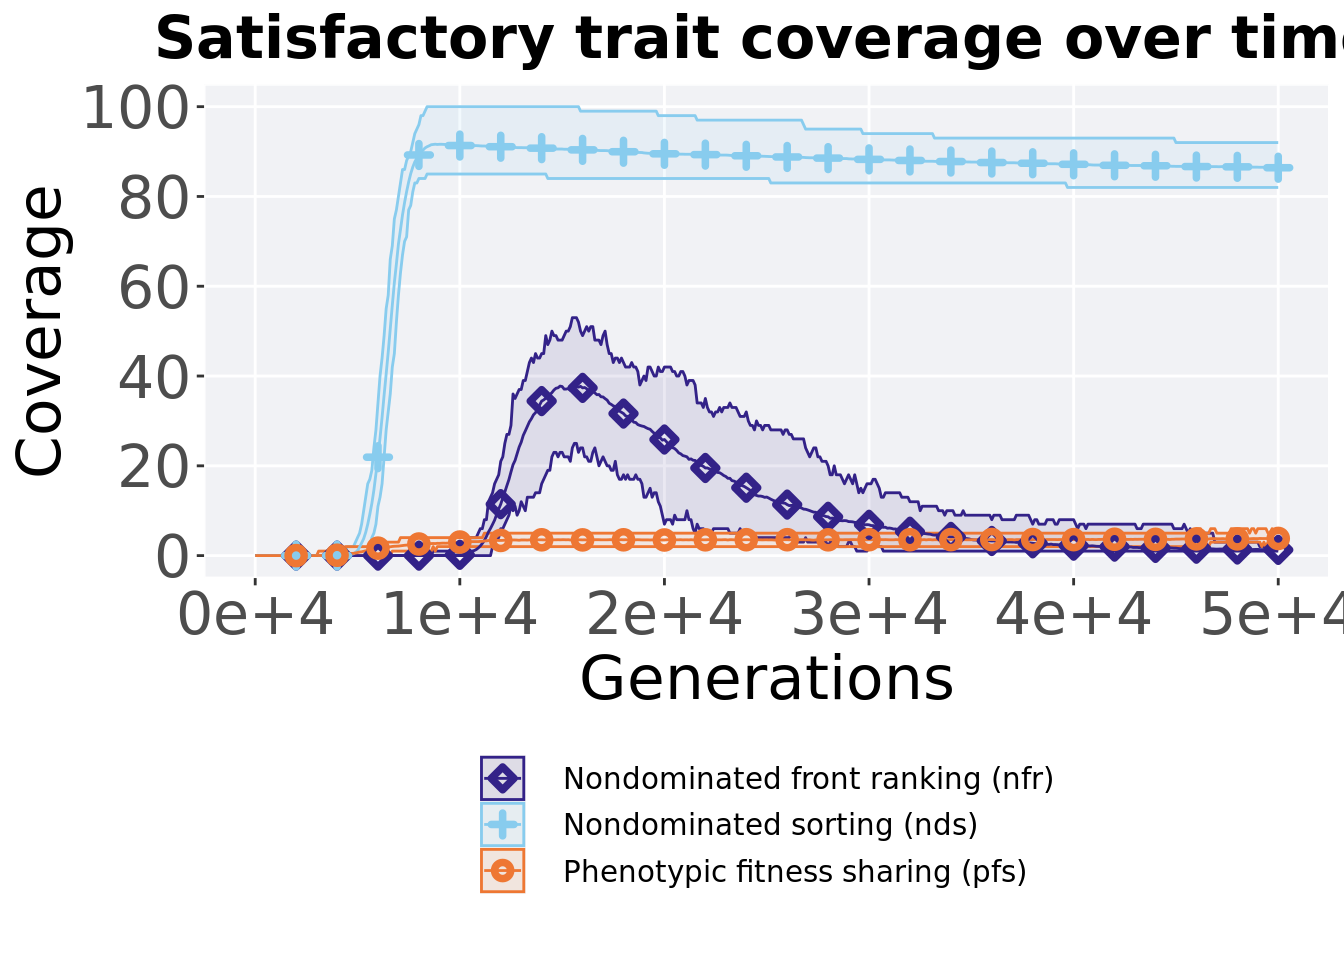
\includegraphics{demo_files/figure-latex/con-nss-sat-ot-1.pdf}

\hypertarget{best-coverage-throughout-1}{%
\subsection{Best coverage throughout}\label{best-coverage-throughout-1}}

Best satisfactory trait coverage.

\begin{Shaded}
\begin{Highlighting}[]
\CommentTok{### best satisfactory trait coverage throughout}
\NormalTok{coverage }\OperatorTok
\StringTok{  }\KeywordTok{ggplot}\NormalTok{(., }\KeywordTok{aes}\NormalTok{(}\DataTypeTok{x =}\NormalTok{ acron, }\DataTypeTok{y =}\NormalTok{ val, }\DataTypeTok{color =}\NormalTok{ acron, }\DataTypeTok{fill =}\NormalTok{ acron, }\DataTypeTok{shape =}\NormalTok{ acron)) }\OperatorTok{+}
\StringTok{  }\KeywordTok{geom_flat_violin}\NormalTok{(}\DataTypeTok{position =} \KeywordTok{position_nudge}\NormalTok{(}\DataTypeTok{x =} \FloatTok{.2}\NormalTok{, }\DataTypeTok{y =} \DecValTok{0}\NormalTok{), }\DataTypeTok{scale =} \StringTok{'width'}\NormalTok{, }\DataTypeTok{alpha =} \FloatTok{0.2}\NormalTok{) }\OperatorTok{+}
\StringTok{  }\KeywordTok{geom_point}\NormalTok{(}\DataTypeTok{position =} \KeywordTok{position_jitter}\NormalTok{(}\DataTypeTok{width =} \FloatTok{.1}\NormalTok{), }\DataTypeTok{size =} \FloatTok{1.5}\NormalTok{, }\DataTypeTok{alpha =} \FloatTok{1.0}\NormalTok{) }\OperatorTok{+}
\StringTok{  }\KeywordTok{geom_boxplot}\NormalTok{(}\DataTypeTok{color =} \StringTok{'black'}\NormalTok{, }\DataTypeTok{width =} \FloatTok{.2}\NormalTok{, }\DataTypeTok{outlier.shape =} \OtherTok{NA}\NormalTok{, }\DataTypeTok{alpha =} \FloatTok{0.0}\NormalTok{) }\OperatorTok{+}
\StringTok{  }\KeywordTok{scale_y_continuous}\NormalTok{(}
    \DataTypeTok{name=}\StringTok{"Coverage"}\NormalTok{,}
    \DataTypeTok{limits=}\KeywordTok{c}\NormalTok{(}\DecValTok{0}\NormalTok{, }\DecValTok{100}\NormalTok{),}
    \DataTypeTok{breaks=}\KeywordTok{seq}\NormalTok{(}\DecValTok{0}\NormalTok{,}\DecValTok{100}\NormalTok{, }\DecValTok{20}\NormalTok{),}
    \DataTypeTok{labels=}\KeywordTok{c}\NormalTok{(}\StringTok{"0"}\NormalTok{, }\StringTok{"20"}\NormalTok{, }\StringTok{"40"}\NormalTok{, }\StringTok{"60"}\NormalTok{, }\StringTok{"80"}\NormalTok{, }\StringTok{"100"}\NormalTok{)}
\NormalTok{  ) }\OperatorTok{+}
\StringTok{  }\KeywordTok{scale_x_discrete}\NormalTok{(}
    \DataTypeTok{name=}\StringTok{"Scheme"}
\NormalTok{  )}\OperatorTok{+}
\StringTok{  }\KeywordTok{scale_shape_manual}\NormalTok{(}\DataTypeTok{values=}\NormalTok{SHAPE)}\OperatorTok{+}
\StringTok{  }\KeywordTok{scale_colour_manual}\NormalTok{(}\DataTypeTok{values =}\NormalTok{ cb_palette, ) }\OperatorTok{+}
\StringTok{  }\KeywordTok{scale_fill_manual}\NormalTok{(}\DataTypeTok{values =}\NormalTok{ cb_palette) }\OperatorTok{+}
\StringTok{  }\KeywordTok{ggtitle}\NormalTok{(}\StringTok{'Best satisfactory trait coverage'}\NormalTok{)}\OperatorTok{+}
\StringTok{  }\NormalTok{p_theme }\OperatorTok{+}\StringTok{ }\KeywordTok{theme}\NormalTok{(}\DataTypeTok{legend.title=}\KeywordTok{element_blank}\NormalTok{()) }\OperatorTok{+}
\StringTok{  }\KeywordTok{guides}\NormalTok{(}
    \DataTypeTok{shape=}\KeywordTok{guide_legend}\NormalTok{(}\DataTypeTok{nrow=}\DecValTok{1}\NormalTok{, }\DataTypeTok{title.position =} \StringTok{"bottom"}\NormalTok{),}
    \DataTypeTok{color=}\KeywordTok{guide_legend}\NormalTok{(}\DataTypeTok{nrow=}\DecValTok{1}\NormalTok{, }\DataTypeTok{title.position =} \StringTok{"bottom"}\NormalTok{),}
    \DataTypeTok{fill=}\KeywordTok{guide_legend}\NormalTok{(}\DataTypeTok{nrow=}\DecValTok{1}\NormalTok{, }\DataTypeTok{title.position =} \StringTok{"bottom"}\NormalTok{)}
\NormalTok{  )}
\end{Highlighting}
\end{Shaded}

\begin{verbatim}
## Warning: Removed 1 rows containing missing values (`geom_point()`).
\end{verbatim}

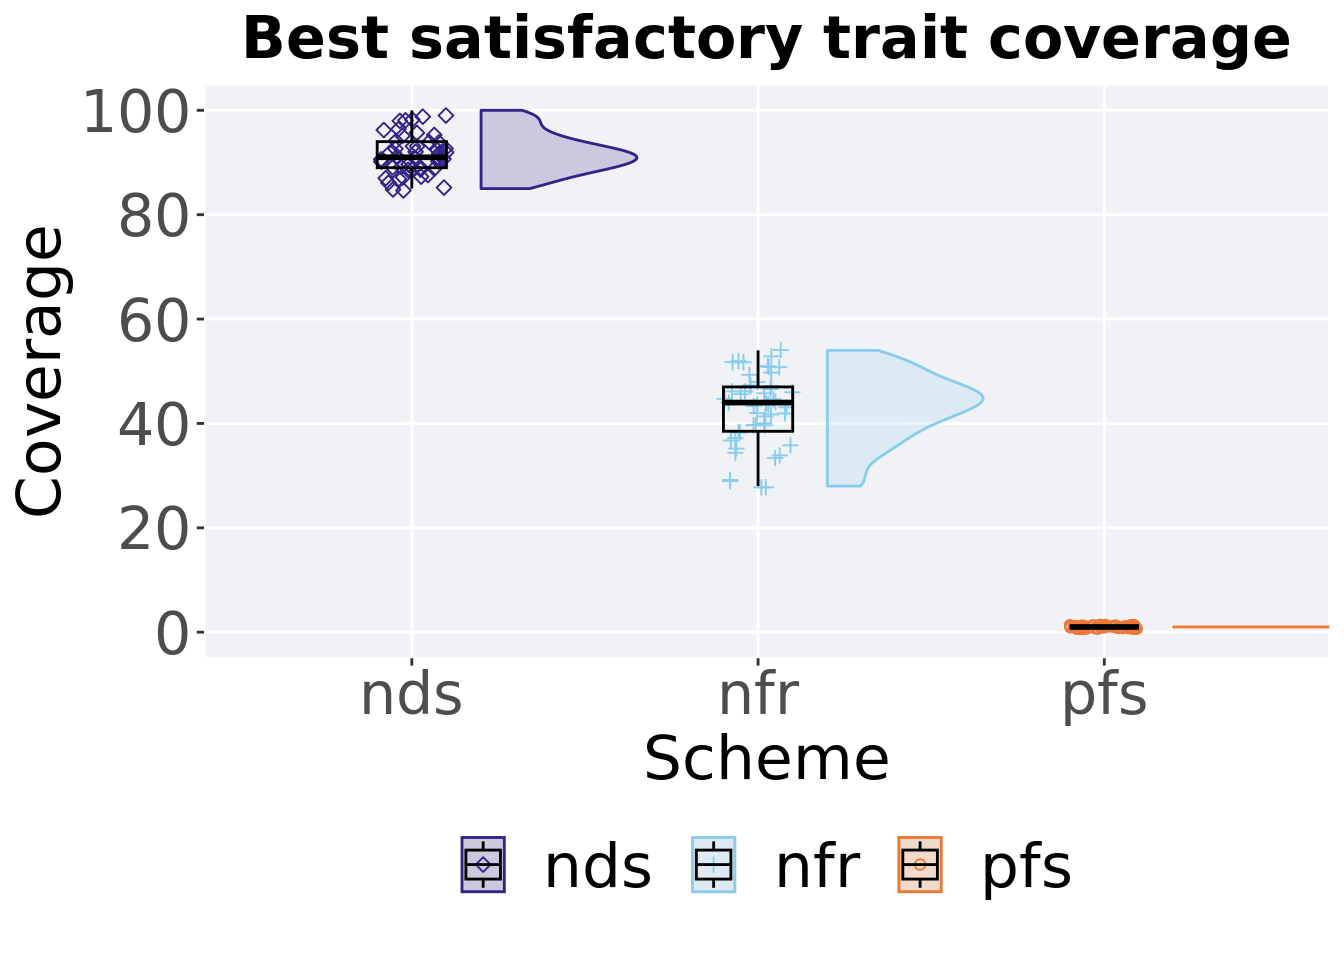
\includegraphics{demo_files/figure-latex/con-nss-sat-bst-1.pdf}

\hypertarget{stats-11}{%
\subsubsection{Stats}\label{stats-11}}

Summary statistics for the best satisfactory trait coverage.

\begin{Shaded}
\begin{Highlighting}[]
\CommentTok{# summary}
\NormalTok{coverage}\OperatorTok{$}\NormalTok{acron =}\StringTok{ }\KeywordTok{factor}\NormalTok{(coverage}\OperatorTok{$}\NormalTok{acron, }\DataTypeTok{levels =} \KeywordTok{c}\NormalTok{(}\StringTok{'nds'}\NormalTok{, }\StringTok{'pfs'}\NormalTok{, }\StringTok{'nfr'}\NormalTok{))}
\NormalTok{coverage }\OperatorTok
\StringTok{  }\KeywordTok{group_by}\NormalTok{(acron) }\OperatorTok
\StringTok{  }\NormalTok{dplyr}\OperatorTok{::}\KeywordTok{summarise}\NormalTok{(}
    \DataTypeTok{count =} \KeywordTok{n}\NormalTok{(),}
    \DataTypeTok{na_cnt =} \KeywordTok{sum}\NormalTok{(}\KeywordTok{is.na}\NormalTok{(val)),}
    \DataTypeTok{min =} \KeywordTok{min}\NormalTok{(val, }\DataTypeTok{na.rm =} \OtherTok{TRUE}\NormalTok{),}
    \DataTypeTok{median =} \KeywordTok{median}\NormalTok{(val, }\DataTypeTok{na.rm =} \OtherTok{TRUE}\NormalTok{),}
    \DataTypeTok{mean =} \KeywordTok{mean}\NormalTok{(val, }\DataTypeTok{na.rm =} \OtherTok{TRUE}\NormalTok{),}
    \DataTypeTok{max =} \KeywordTok{max}\NormalTok{(val, }\DataTypeTok{na.rm =} \OtherTok{TRUE}\NormalTok{),}
    \DataTypeTok{IQR =} \KeywordTok{IQR}\NormalTok{(val, }\DataTypeTok{na.rm =} \OtherTok{TRUE}\NormalTok{)}
\NormalTok{  )}
\end{Highlighting}
\end{Shaded}

\begin{verbatim}
## # A tibble: 3 x 8
##   acron count na_cnt   min median  mean   max   IQR
##   <fct> <int>  <int> <dbl>  <dbl> <dbl> <dbl> <dbl>
## 1 nds      50      0    85     91  91.8   100   5  
## 2 pfs      50      0     1      1   1       1   0  
## 3 nfr      50      0    28     44  42.8    54   8.5
\end{verbatim}

Kruskal--Wallis test provides evidence of difference among best satisfactory trait coverage.

\begin{Shaded}
\begin{Highlighting}[]
\KeywordTok{kruskal.test}\NormalTok{(val }\OperatorTok{~}\StringTok{ }\NormalTok{acron,}\DataTypeTok{data =}\NormalTok{ coverage)}
\end{Highlighting}
\end{Shaded}

\begin{verbatim}
## 
##  Kruskal-Wallis rank sum test
## 
## data:  val by acron
## Kruskal-Wallis chi-squared = 137.61, df = 2, p-value < 2.2e-16
\end{verbatim}

Results for post-hoc Wilcoxon rank-sum test with a Bonferroni correction on best satisfactory trait coverage.

\begin{Shaded}
\begin{Highlighting}[]
\KeywordTok{pairwise.wilcox.test}\NormalTok{(}\DataTypeTok{x =}\NormalTok{ coverage}\OperatorTok{$}\NormalTok{val, }\DataTypeTok{g =}\NormalTok{ coverage}\OperatorTok{$}\NormalTok{acron, }\DataTypeTok{p.adjust.method =} \StringTok{"bonferroni"}\NormalTok{,}
                     \DataTypeTok{paired =} \OtherTok{FALSE}\NormalTok{, }\DataTypeTok{conf.int =} \OtherTok{FALSE}\NormalTok{, }\DataTypeTok{alternative =} \StringTok{'l'}\NormalTok{)}
\end{Highlighting}
\end{Shaded}

\begin{verbatim}
## 
##  Pairwise comparisons using Wilcoxon rank sum test with continuity correction 
## 
## data:  coverage$val and coverage$acron 
## 
##     nds    pfs
## pfs <2e-16 -  
## nfr <2e-16 1  
## 
## P value adjustment method: bonferroni
\end{verbatim}

\hypertarget{end-of-50000-generations-2}{%
\subsection{End of 50,000 generations}\label{end-of-50000-generations-2}}

Satisfactory trait coverage in the population at the end of 50,000 generations.

\begin{Shaded}
\begin{Highlighting}[]
\NormalTok{coverage }\OperatorTok
\StringTok{  }\KeywordTok{ggplot}\NormalTok{(., }\KeywordTok{aes}\NormalTok{(}\DataTypeTok{x =}\NormalTok{ acron, }\DataTypeTok{y =}\NormalTok{ pop_uni_obj, }\DataTypeTok{color =}\NormalTok{ acron, }\DataTypeTok{fill =}\NormalTok{ acron, }\DataTypeTok{shape =}\NormalTok{ acron)) }\OperatorTok{+}
\StringTok{  }\KeywordTok{geom_flat_violin}\NormalTok{(}\DataTypeTok{position =} \KeywordTok{position_nudge}\NormalTok{(}\DataTypeTok{x =} \FloatTok{.2}\NormalTok{, }\DataTypeTok{y =} \DecValTok{0}\NormalTok{), }\DataTypeTok{scale =} \StringTok{'width'}\NormalTok{, }\DataTypeTok{alpha =} \FloatTok{0.2}\NormalTok{) }\OperatorTok{+}
\StringTok{  }\KeywordTok{geom_point}\NormalTok{(}\DataTypeTok{position =} \KeywordTok{position_jitter}\NormalTok{(}\DataTypeTok{width =} \FloatTok{.1}\NormalTok{), }\DataTypeTok{size =} \FloatTok{1.5}\NormalTok{, }\DataTypeTok{alpha =} \FloatTok{1.0}\NormalTok{) }\OperatorTok{+}
\StringTok{  }\KeywordTok{geom_boxplot}\NormalTok{(}\DataTypeTok{color =} \StringTok{'black'}\NormalTok{, }\DataTypeTok{width =} \FloatTok{.2}\NormalTok{, }\DataTypeTok{outlier.shape =} \OtherTok{NA}\NormalTok{, }\DataTypeTok{alpha =} \FloatTok{0.0}\NormalTok{) }\OperatorTok{+}
\StringTok{  }\KeywordTok{scale_y_continuous}\NormalTok{(}
    \DataTypeTok{name=}\StringTok{"Coverage"}\NormalTok{,}
    \DataTypeTok{limits=}\KeywordTok{c}\NormalTok{(}\DecValTok{0}\NormalTok{, }\DecValTok{100}\NormalTok{),}
    \DataTypeTok{breaks=}\KeywordTok{seq}\NormalTok{(}\DecValTok{0}\NormalTok{,}\DecValTok{100}\NormalTok{, }\DecValTok{20}\NormalTok{),}
    \DataTypeTok{labels=}\KeywordTok{c}\NormalTok{(}\StringTok{"0"}\NormalTok{, }\StringTok{"20"}\NormalTok{, }\StringTok{"40"}\NormalTok{, }\StringTok{"60"}\NormalTok{, }\StringTok{"80"}\NormalTok{, }\StringTok{"100"}\NormalTok{)}
\NormalTok{  ) }\OperatorTok{+}
\StringTok{  }\KeywordTok{scale_x_discrete}\NormalTok{(}
    \DataTypeTok{name=}\StringTok{"Scheme"}
\NormalTok{  )}\OperatorTok{+}
\StringTok{  }\KeywordTok{scale_shape_manual}\NormalTok{(}\DataTypeTok{values=}\NormalTok{SHAPE)}\OperatorTok{+}
\StringTok{  }\KeywordTok{scale_colour_manual}\NormalTok{(}\DataTypeTok{values =}\NormalTok{ cb_palette, ) }\OperatorTok{+}
\StringTok{  }\KeywordTok{scale_fill_manual}\NormalTok{(}\DataTypeTok{values =}\NormalTok{ cb_palette) }\OperatorTok{+}
\StringTok{  }\KeywordTok{ggtitle}\NormalTok{(}\StringTok{'Final satisfactory trait coverage'}\NormalTok{)}\OperatorTok{+}
\StringTok{  }\NormalTok{p_theme }\OperatorTok{+}\StringTok{ }\KeywordTok{theme}\NormalTok{(}\DataTypeTok{legend.title=}\KeywordTok{element_blank}\NormalTok{()) }\OperatorTok{+}
\StringTok{  }\KeywordTok{guides}\NormalTok{(}
    \DataTypeTok{shape=}\KeywordTok{guide_legend}\NormalTok{(}\DataTypeTok{nrow=}\DecValTok{1}\NormalTok{, }\DataTypeTok{title.position =} \StringTok{"bottom"}\NormalTok{),}
    \DataTypeTok{color=}\KeywordTok{guide_legend}\NormalTok{(}\DataTypeTok{nrow=}\DecValTok{1}\NormalTok{, }\DataTypeTok{title.position =} \StringTok{"bottom"}\NormalTok{),}
    \DataTypeTok{fill=}\KeywordTok{guide_legend}\NormalTok{(}\DataTypeTok{nrow=}\DecValTok{1}\NormalTok{, }\DataTypeTok{title.position =} \StringTok{"bottom"}\NormalTok{)}
\NormalTok{  )}
\end{Highlighting}
\end{Shaded}

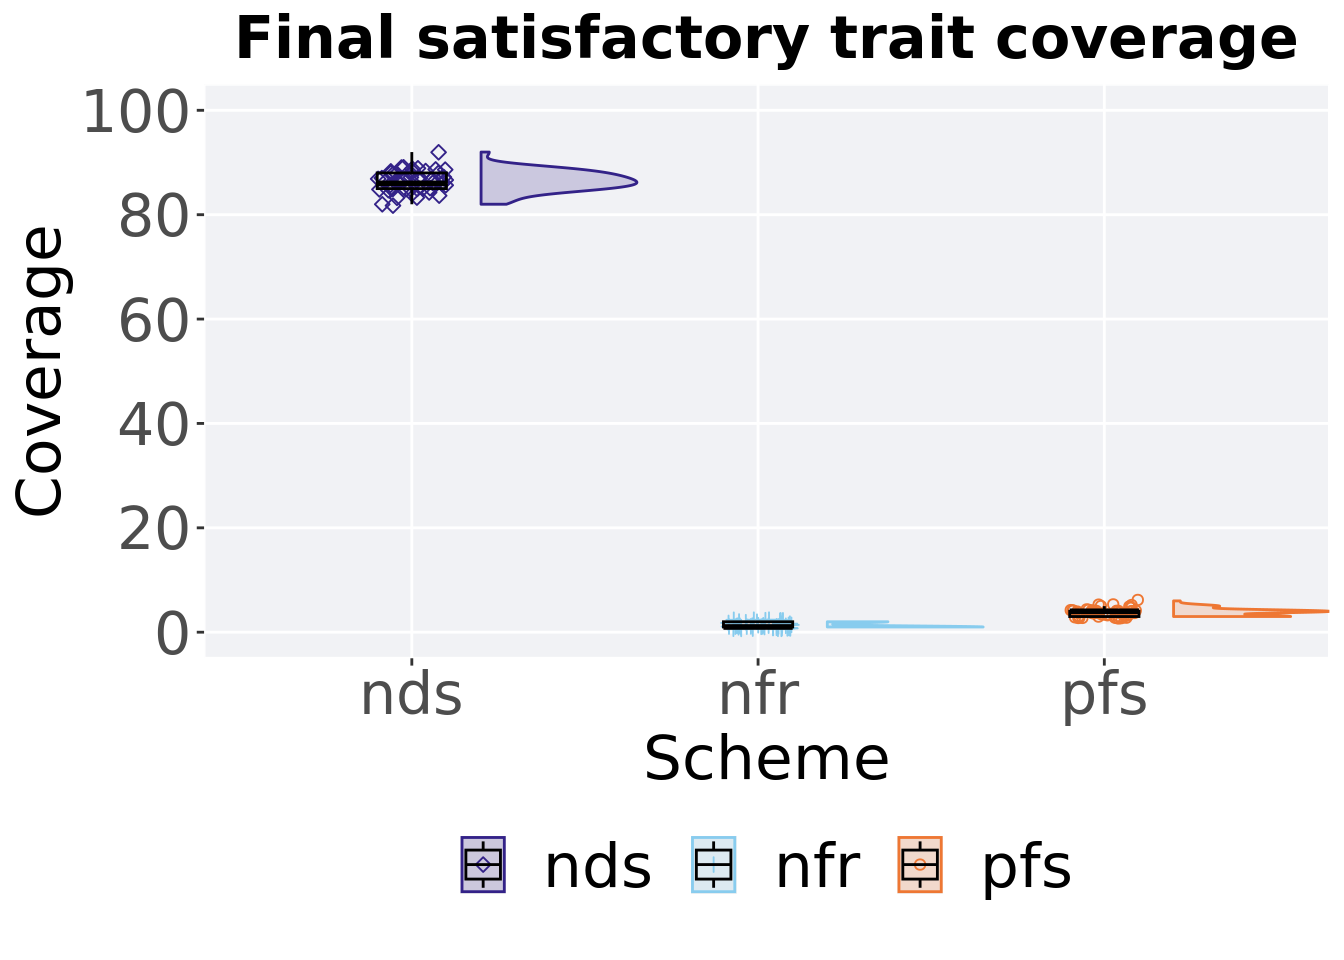
\includegraphics{demo_files/figure-latex/con-nss-sat-end-1.pdf}

\hypertarget{stats-12}{%
\subsubsection{Stats}\label{stats-12}}

Summary statistics for satisfactory trait coverage in the population at the end of 50,000 generations.

\begin{Shaded}
\begin{Highlighting}[]
\NormalTok{coverage}\OperatorTok{$}\NormalTok{acron =}\StringTok{ }\KeywordTok{factor}\NormalTok{(coverage}\OperatorTok{$}\NormalTok{acron, }\DataTypeTok{levels =} \KeywordTok{c}\NormalTok{(}\StringTok{'nds'}\NormalTok{, }\StringTok{'pfs'}\NormalTok{, }\StringTok{'nfr'}\NormalTok{))}
\NormalTok{coverage }\OperatorTok
\StringTok{  }\KeywordTok{group_by}\NormalTok{(acron) }\OperatorTok
\StringTok{  }\NormalTok{dplyr}\OperatorTok{::}\KeywordTok{summarise}\NormalTok{(}
    \DataTypeTok{count =} \KeywordTok{n}\NormalTok{(),}
    \DataTypeTok{na_cnt =} \KeywordTok{sum}\NormalTok{(}\KeywordTok{is.na}\NormalTok{(pop_uni_obj)),}
    \DataTypeTok{min =} \KeywordTok{min}\NormalTok{(pop_uni_obj, }\DataTypeTok{na.rm =} \OtherTok{TRUE}\NormalTok{),}
    \DataTypeTok{median =} \KeywordTok{median}\NormalTok{(pop_uni_obj, }\DataTypeTok{na.rm =} \OtherTok{TRUE}\NormalTok{),}
    \DataTypeTok{mean =} \KeywordTok{mean}\NormalTok{(pop_uni_obj, }\DataTypeTok{na.rm =} \OtherTok{TRUE}\NormalTok{),}
    \DataTypeTok{max =} \KeywordTok{max}\NormalTok{(pop_uni_obj, }\DataTypeTok{na.rm =} \OtherTok{TRUE}\NormalTok{),}
    \DataTypeTok{IQR =} \KeywordTok{IQR}\NormalTok{(pop_uni_obj, }\DataTypeTok{na.rm =} \OtherTok{TRUE}\NormalTok{)}
\NormalTok{  )}
\end{Highlighting}
\end{Shaded}

\begin{verbatim}
## # A tibble: 3 x 8
##   acron count na_cnt   min median  mean   max   IQR
##   <fct> <int>  <int> <int>  <dbl> <dbl> <int> <dbl>
## 1 nds      50      0    82     86 86.4     92     3
## 2 pfs      50      0     3      4  3.82     6     1
## 3 nfr      50      0     1      1  1.28     2     1
\end{verbatim}

Kruskal--Wallis test provides evidence of difference among satisfactory trait coverage in the population at the end of 50,000 generations.

\begin{Shaded}
\begin{Highlighting}[]
\KeywordTok{kruskal.test}\NormalTok{(pop_uni_obj }\OperatorTok{~}\StringTok{ }\NormalTok{acron,}\DataTypeTok{data =}\NormalTok{ coverage)}
\end{Highlighting}
\end{Shaded}

\begin{verbatim}
## 
##  Kruskal-Wallis rank sum test
## 
## data:  pop_uni_obj by acron
## Kruskal-Wallis chi-squared = 135.36, df = 2, p-value < 2.2e-16
\end{verbatim}

Results for post-hoc Wilcoxon rank-sum test with a Bonferroni correction on satisfactory trait coverage in the population at the end of 50,000 generations.

\begin{Shaded}
\begin{Highlighting}[]
\KeywordTok{pairwise.wilcox.test}\NormalTok{(}\DataTypeTok{x =}\NormalTok{ coverage}\OperatorTok{$}\NormalTok{pop_uni_obj, }\DataTypeTok{g =}\NormalTok{ coverage}\OperatorTok{$}\NormalTok{acron, }\DataTypeTok{p.adjust.method =} \StringTok{"bonferroni"}\NormalTok{,}
                     \DataTypeTok{paired =} \OtherTok{FALSE}\NormalTok{, }\DataTypeTok{conf.int =} \OtherTok{FALSE}\NormalTok{, }\DataTypeTok{alternative =} \StringTok{'l'}\NormalTok{)}
\end{Highlighting}
\end{Shaded}

\begin{verbatim}
## 
##  Pairwise comparisons using Wilcoxon rank sum test with continuity correction 
## 
## data:  coverage$pop_uni_obj and coverage$acron 
## 
##     nds    pfs   
## pfs <2e-16 -     
## nfr <2e-16 <2e-16
## 
## P value adjustment method: bonferroni
\end{verbatim}

\hypertarget{multi-valley-crossing-results-2}{%
\section{Multi-valley crossing results}\label{multi-valley-crossing-results-2}}

\hypertarget{satisfactory-trait-coverage-1}{%
\subsection{Satisfactory trait coverage}\label{satisfactory-trait-coverage-1}}

Satisfactory trait coverage analysis.

\hypertarget{coverage-over-time-2}{%
\subsubsection{Coverage over time}\label{coverage-over-time-2}}

Satisfactory trait coverage over time.

\begin{Shaded}
\begin{Highlighting}[]
\CommentTok{# data for lines and shading on plots}
\NormalTok{lines =}\StringTok{ }\KeywordTok{filter}\NormalTok{(cc_over_time_mvc, diagnostic }\OperatorTok{==}\StringTok{ 'contradictory_objectives'}\NormalTok{) }\OperatorTok
\StringTok{  }\KeywordTok{group_by}\NormalTok{(}\StringTok{`}\DataTypeTok{Selection}\CharTok{\textbackslash{}n}\DataTypeTok{Scheme}\StringTok{`}\NormalTok{, gen) }\OperatorTok
\StringTok{  }\NormalTok{dplyr}\OperatorTok{::}\KeywordTok{summarise}\NormalTok{(}
    \DataTypeTok{min =} \KeywordTok{min}\NormalTok{(pop_uni_obj),}
    \DataTypeTok{mean =} \KeywordTok{mean}\NormalTok{(pop_uni_obj),}
    \DataTypeTok{max =} \KeywordTok{max}\NormalTok{(pop_uni_obj)}
\NormalTok{  )}
\end{Highlighting}
\end{Shaded}

\begin{verbatim}
## `summarise()` has grouped output by 'Selection Scheme'. You can override using
## the `.groups` argument.
\end{verbatim}

\begin{Shaded}
\begin{Highlighting}[]
\KeywordTok{ggplot}\NormalTok{(lines, }\KeywordTok{aes}\NormalTok{(}\DataTypeTok{x=}\NormalTok{gen, }\DataTypeTok{y=}\NormalTok{mean, }\DataTypeTok{group =} \StringTok{`}\DataTypeTok{Selection}\CharTok{\textbackslash{}n}\DataTypeTok{Scheme}\StringTok{`}\NormalTok{, }\DataTypeTok{fill =}\StringTok{`}\DataTypeTok{Selection}\CharTok{\textbackslash{}n}\DataTypeTok{Scheme}\StringTok{`}\NormalTok{, }\DataTypeTok{color =} \StringTok{`}\DataTypeTok{Selection}\CharTok{\textbackslash{}n}\DataTypeTok{Scheme}\StringTok{`}\NormalTok{, }\DataTypeTok{shape =} \StringTok{`}\DataTypeTok{Selection}\CharTok{\textbackslash{}n}\DataTypeTok{Scheme}\StringTok{`}\NormalTok{)) }\OperatorTok{+}
\StringTok{  }\KeywordTok{geom_ribbon}\NormalTok{(}\KeywordTok{aes}\NormalTok{(}\DataTypeTok{ymin =}\NormalTok{ min, }\DataTypeTok{ymax =}\NormalTok{ max), }\DataTypeTok{alpha =} \FloatTok{0.1}\NormalTok{) }\OperatorTok{+}
\StringTok{  }\KeywordTok{geom_line}\NormalTok{(}\DataTypeTok{size =} \FloatTok{0.5}\NormalTok{) }\OperatorTok{+}
\StringTok{  }\KeywordTok{geom_point}\NormalTok{(}\DataTypeTok{data =} \KeywordTok{filter}\NormalTok{(lines, gen }\OperatorTok\StringTok{ }\DecValTok{2000} \OperatorTok{==}\StringTok{ }\DecValTok{0} \OperatorTok{&}\StringTok{ }\NormalTok{gen }\OperatorTok{!=}\StringTok{ }\DecValTok{0}\NormalTok{), }\DataTypeTok{size =} \FloatTok{1.5}\NormalTok{, }\DataTypeTok{stroke =} \FloatTok{2.0}\NormalTok{, }\DataTypeTok{alpha =} \FloatTok{1.0}\NormalTok{) }\OperatorTok{+}
\StringTok{  }\KeywordTok{scale_y_continuous}\NormalTok{(}
    \DataTypeTok{name=}\StringTok{"Coverage"}\NormalTok{,}
    \DataTypeTok{limits=}\KeywordTok{c}\NormalTok{(}\DecValTok{0}\NormalTok{, }\DecValTok{5}\NormalTok{),}
    \DataTypeTok{breaks=}\KeywordTok{seq}\NormalTok{(}\DecValTok{0}\NormalTok{,}\DecValTok{5}\NormalTok{, }\DecValTok{1}\NormalTok{)}
\NormalTok{  ) }\OperatorTok{+}
\StringTok{  }\KeywordTok{scale_x_continuous}\NormalTok{(}
    \DataTypeTok{name=}\StringTok{"Generations"}\NormalTok{,}
    \DataTypeTok{limits=}\KeywordTok{c}\NormalTok{(}\DecValTok{0}\NormalTok{, }\DecValTok{50000}\NormalTok{),}
    \DataTypeTok{breaks=}\KeywordTok{c}\NormalTok{(}\DecValTok{0}\NormalTok{, }\DecValTok{10000}\NormalTok{, }\DecValTok{20000}\NormalTok{, }\DecValTok{30000}\NormalTok{, }\DecValTok{40000}\NormalTok{, }\DecValTok{50000}\NormalTok{),}
    \DataTypeTok{labels=}\KeywordTok{c}\NormalTok{(}\StringTok{"0e+4"}\NormalTok{, }\StringTok{"1e+4"}\NormalTok{, }\StringTok{"2e+4"}\NormalTok{, }\StringTok{"3e+4"}\NormalTok{, }\StringTok{"4e+4"}\NormalTok{, }\StringTok{"5e+4"}\NormalTok{)}
\NormalTok{  ) }\OperatorTok{+}
\StringTok{  }\KeywordTok{scale_shape_manual}\NormalTok{(}\DataTypeTok{values=}\NormalTok{SHAPE)}\OperatorTok{+}
\StringTok{  }\KeywordTok{scale_colour_manual}\NormalTok{(}\DataTypeTok{values =}\NormalTok{ cb_palette) }\OperatorTok{+}
\StringTok{  }\KeywordTok{scale_fill_manual}\NormalTok{(}\DataTypeTok{values =}\NormalTok{ cb_palette) }\OperatorTok{+}
\StringTok{  }\KeywordTok{ggtitle}\NormalTok{(}\StringTok{'Satisfactory trait coverage over time'}\NormalTok{)}\OperatorTok{+}
\StringTok{  }\NormalTok{p_theme }\OperatorTok{+}\StringTok{ }\KeywordTok{theme}\NormalTok{(}\DataTypeTok{legend.title=}\KeywordTok{element_blank}\NormalTok{(),}\DataTypeTok{legend.text=}\KeywordTok{element_text}\NormalTok{(}\DataTypeTok{size=}\DecValTok{11}\NormalTok{)) }\OperatorTok{+}
\StringTok{  }\KeywordTok{guides}\NormalTok{(}
    \DataTypeTok{shape=}\KeywordTok{guide_legend}\NormalTok{(}\DataTypeTok{ncol=}\DecValTok{2}\NormalTok{, }\DataTypeTok{title.position =} \StringTok{"bottom"}\NormalTok{),}
    \DataTypeTok{color=}\KeywordTok{guide_legend}\NormalTok{(}\DataTypeTok{ncol=}\DecValTok{2}\NormalTok{, }\DataTypeTok{title.position =} \StringTok{"bottom"}\NormalTok{),}
    \DataTypeTok{fill=}\KeywordTok{guide_legend}\NormalTok{(}\DataTypeTok{ncol=}\DecValTok{2}\NormalTok{, }\DataTypeTok{title.position =} \StringTok{"bottom"}\NormalTok{)}
\NormalTok{  )}
\end{Highlighting}
\end{Shaded}

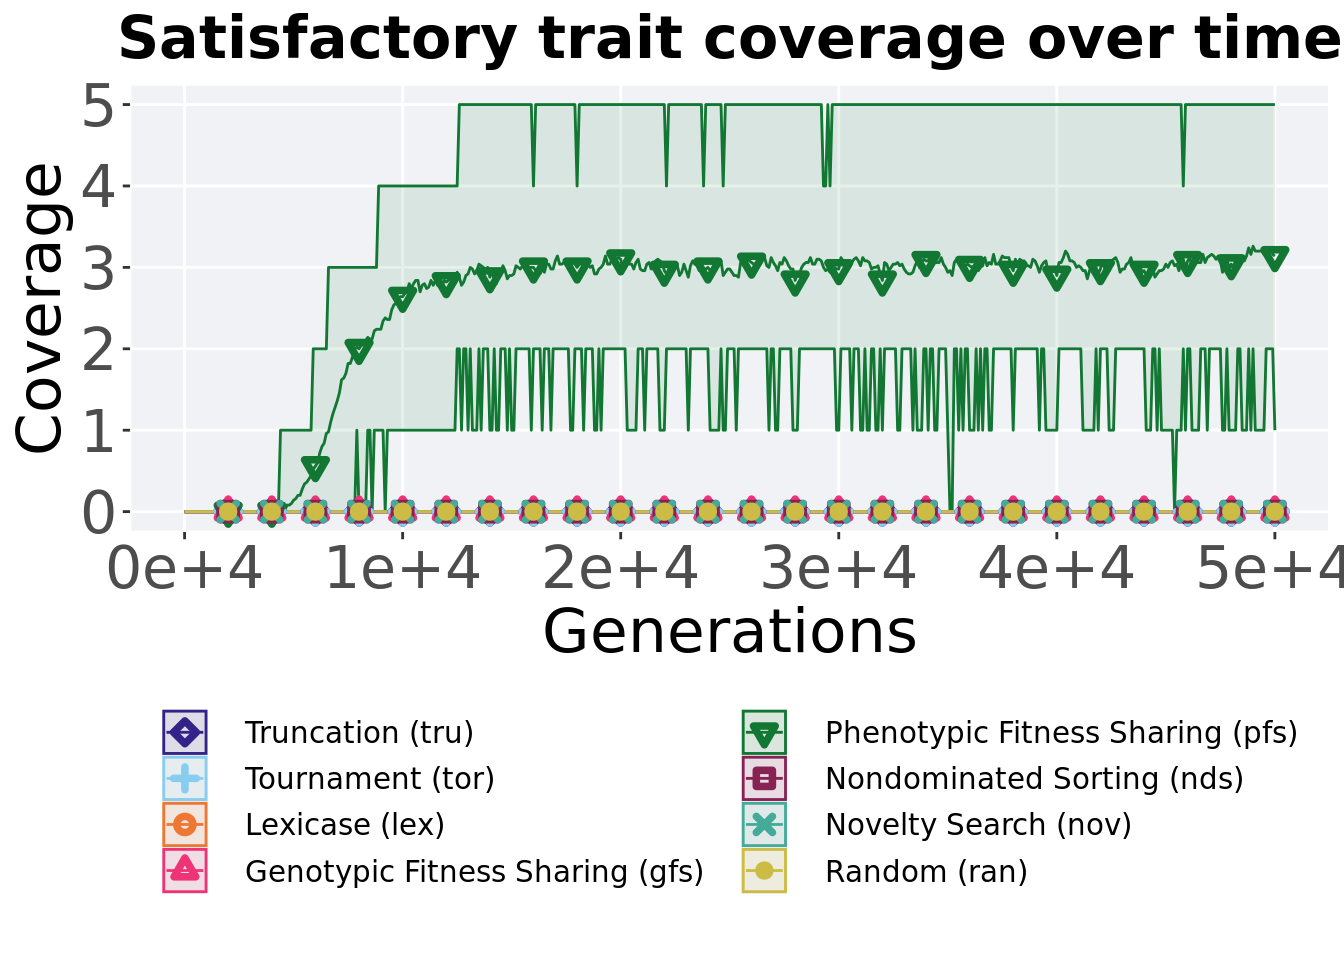
\includegraphics{demo_files/figure-latex/con-mvc-sat-ot-1.pdf}

\hypertarget{best-coverage-throughout-2}{%
\subsubsection{Best coverage throughout}\label{best-coverage-throughout-2}}

Best satisfactory trait coverage throughout 50,000 generations.

\begin{Shaded}
\begin{Highlighting}[]
\CommentTok{### best satisfactory trait coverage throughout}
\KeywordTok{filter}\NormalTok{(cc_best_mvc, col }\OperatorTok{==}\StringTok{ 'pop_uni_obj'} \OperatorTok{&}\StringTok{ }\NormalTok{diagnostic }\OperatorTok{==}\StringTok{ 'contradictory_objectives'}\NormalTok{) }\OperatorTok
\StringTok{  }\KeywordTok{ggplot}\NormalTok{(., }\KeywordTok{aes}\NormalTok{(}\DataTypeTok{x =}\NormalTok{ acron, }\DataTypeTok{y =}\NormalTok{ val, }\DataTypeTok{color =}\NormalTok{ acron, }\DataTypeTok{fill =}\NormalTok{ acron, }\DataTypeTok{shape =}\NormalTok{ acron)) }\OperatorTok{+}
\StringTok{  }\KeywordTok{geom_flat_violin}\NormalTok{(}\DataTypeTok{position =} \KeywordTok{position_nudge}\NormalTok{(}\DataTypeTok{x =} \FloatTok{.2}\NormalTok{, }\DataTypeTok{y =} \DecValTok{0}\NormalTok{), }\DataTypeTok{scale =} \StringTok{'width'}\NormalTok{, }\DataTypeTok{alpha =} \FloatTok{0.2}\NormalTok{) }\OperatorTok{+}
\StringTok{  }\KeywordTok{geom_point}\NormalTok{(}\DataTypeTok{position =} \KeywordTok{position_jitter}\NormalTok{(}\DataTypeTok{width =} \FloatTok{.1}\NormalTok{), }\DataTypeTok{size =} \FloatTok{1.5}\NormalTok{, }\DataTypeTok{alpha =} \FloatTok{1.0}\NormalTok{) }\OperatorTok{+}
\StringTok{  }\KeywordTok{geom_boxplot}\NormalTok{(}\DataTypeTok{color =} \StringTok{'black'}\NormalTok{, }\DataTypeTok{width =} \FloatTok{.2}\NormalTok{, }\DataTypeTok{outlier.shape =} \OtherTok{NA}\NormalTok{, }\DataTypeTok{alpha =} \FloatTok{0.0}\NormalTok{) }\OperatorTok{+}
\StringTok{  }\KeywordTok{guides}\NormalTok{(}\DataTypeTok{fill =} \StringTok{"none"}\NormalTok{,}\DataTypeTok{color =} \StringTok{'none'}\NormalTok{, }\DataTypeTok{shape =} \StringTok{'none'}\NormalTok{) }\OperatorTok{+}
\StringTok{  }\KeywordTok{scale_y_continuous}\NormalTok{(}
    \DataTypeTok{name=}\StringTok{"Coverage"}\NormalTok{,}
    \DataTypeTok{limits=}\KeywordTok{c}\NormalTok{(}\DecValTok{0}\NormalTok{, }\DecValTok{5}\NormalTok{)}
\NormalTok{  ) }\OperatorTok{+}
\StringTok{  }\KeywordTok{scale_x_discrete}\NormalTok{(}
    \DataTypeTok{name=}\StringTok{"Scheme"}
\NormalTok{  )}\OperatorTok{+}
\StringTok{  }\KeywordTok{scale_shape_manual}\NormalTok{(}\DataTypeTok{values=}\NormalTok{SHAPE)}\OperatorTok{+}
\StringTok{  }\KeywordTok{scale_colour_manual}\NormalTok{(}\DataTypeTok{values =}\NormalTok{ cb_palette, ) }\OperatorTok{+}
\StringTok{  }\KeywordTok{scale_fill_manual}\NormalTok{(}\DataTypeTok{values =}\NormalTok{ cb_palette) }\OperatorTok{+}
\StringTok{  }\KeywordTok{ggtitle}\NormalTok{(}\StringTok{'Best satisfactory trait coverage'}\NormalTok{)}\OperatorTok{+}
\StringTok{  }\NormalTok{p_theme }\OperatorTok{+}\StringTok{ }\KeywordTok{theme}\NormalTok{(}\DataTypeTok{legend.title=}\KeywordTok{element_blank}\NormalTok{()) }\OperatorTok{+}
\StringTok{  }\KeywordTok{guides}\NormalTok{(}
    \DataTypeTok{shape=}\KeywordTok{guide_legend}\NormalTok{(}\DataTypeTok{nrow=}\DecValTok{2}\NormalTok{, }\DataTypeTok{title.position =} \StringTok{"bottom"}\NormalTok{),}
    \DataTypeTok{color=}\KeywordTok{guide_legend}\NormalTok{(}\DataTypeTok{nrow=}\DecValTok{2}\NormalTok{, }\DataTypeTok{title.position =} \StringTok{"bottom"}\NormalTok{),}
    \DataTypeTok{fill=}\KeywordTok{guide_legend}\NormalTok{(}\DataTypeTok{nrow=}\DecValTok{2}\NormalTok{, }\DataTypeTok{title.position =} \StringTok{"bottom"}\NormalTok{)}
\NormalTok{  )}
\end{Highlighting}
\end{Shaded}

\begin{verbatim}
## Warning: Removed 171 rows containing missing values (`geom_point()`).
\end{verbatim}

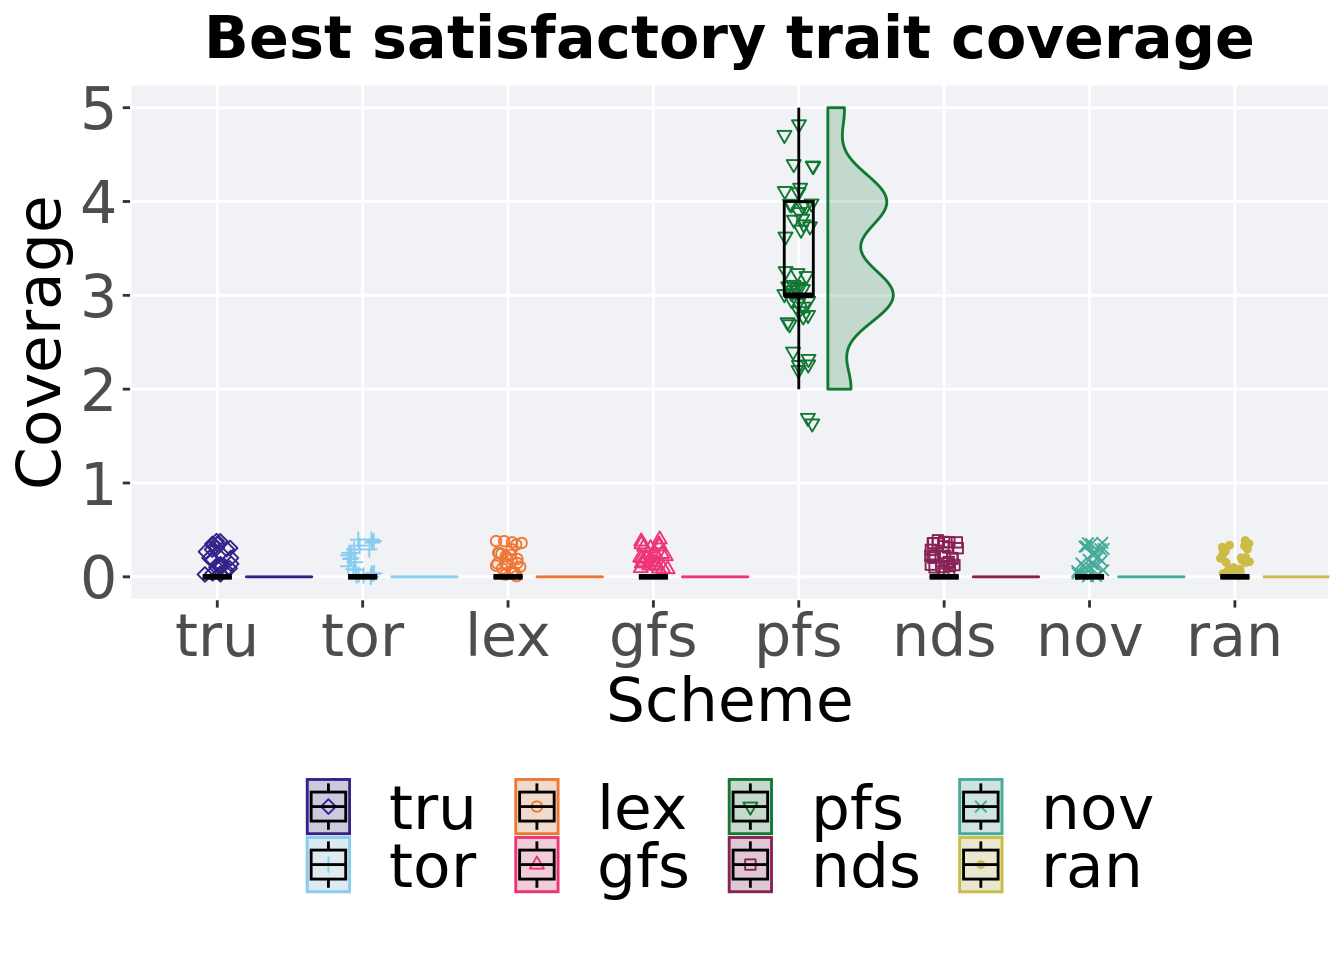
\includegraphics{demo_files/figure-latex/con-mvc-sat-bst-1.pdf}

\hypertarget{stats-13}{%
\paragraph{Stats}\label{stats-13}}

Summary statistics for the best satisfactory trait coverage.

\begin{Shaded}
\begin{Highlighting}[]
\CommentTok{### best}
\NormalTok{coverage =}\StringTok{ }\KeywordTok{filter}\NormalTok{(cc_best_mvc, col }\OperatorTok{==}\StringTok{ 'pop_uni_obj'} \OperatorTok{&}\StringTok{ }\NormalTok{diagnostic }\OperatorTok{==}\StringTok{ 'contradictory_objectives'}\NormalTok{)}
\NormalTok{coverage}\OperatorTok{$}\NormalTok{acron =}\StringTok{ }\KeywordTok{factor}\NormalTok{(coverage}\OperatorTok{$}\NormalTok{acron, }\DataTypeTok{levels =} \KeywordTok{c}\NormalTok{(}\StringTok{'pfs'}\NormalTok{,}\StringTok{'nds'}\NormalTok{, }\StringTok{'lex'}\NormalTok{,  }\StringTok{'gfs'}\NormalTok{, }\StringTok{'tor'}\NormalTok{, }\StringTok{'tru'}\NormalTok{, }\StringTok{'nov'}\NormalTok{, }\StringTok{'ran'}\NormalTok{))}
\NormalTok{coverage }\OperatorTok
\StringTok{  }\KeywordTok{group_by}\NormalTok{(acron) }\OperatorTok
\StringTok{  }\NormalTok{dplyr}\OperatorTok{::}\KeywordTok{summarise}\NormalTok{(}
    \DataTypeTok{count =} \KeywordTok{n}\NormalTok{(),}
    \DataTypeTok{na_cnt =} \KeywordTok{sum}\NormalTok{(}\KeywordTok{is.na}\NormalTok{(val)),}
    \DataTypeTok{min =} \KeywordTok{min}\NormalTok{(val, }\DataTypeTok{na.rm =} \OtherTok{TRUE}\NormalTok{),}
    \DataTypeTok{median =} \KeywordTok{median}\NormalTok{(val, }\DataTypeTok{na.rm =} \OtherTok{TRUE}\NormalTok{),}
    \DataTypeTok{mean =} \KeywordTok{mean}\NormalTok{(val, }\DataTypeTok{na.rm =} \OtherTok{TRUE}\NormalTok{),}
    \DataTypeTok{max =} \KeywordTok{max}\NormalTok{(val, }\DataTypeTok{na.rm =} \OtherTok{TRUE}\NormalTok{),}
    \DataTypeTok{IQR =} \KeywordTok{IQR}\NormalTok{(val, }\DataTypeTok{na.rm =} \OtherTok{TRUE}\NormalTok{)}
\NormalTok{  )}
\end{Highlighting}
\end{Shaded}

\begin{verbatim}
## # A tibble: 8 x 8
##   acron count na_cnt   min median  mean   max   IQR
##   <fct> <int>  <int> <dbl>  <dbl> <dbl> <dbl> <dbl>
## 1 pfs      50      0     2      3  3.42     5     1
## 2 nds      50      0     0      0  0        0     0
## 3 lex      50      0     0      0  0        0     0
## 4 gfs      50      0     0      0  0        0     0
## 5 tor      50      0     0      0  0        0     0
## 6 tru      50      0     0      0  0        0     0
## 7 nov      50      0     0      0  0        0     0
## 8 ran      50      0     0      0  0        0     0
\end{verbatim}

Kruskal--Wallis test provides evidence of difference among satisfactory trait coverage.

\begin{Shaded}
\begin{Highlighting}[]
\KeywordTok{kruskal.test}\NormalTok{(val }\OperatorTok{~}\StringTok{ }\NormalTok{acron, }\DataTypeTok{data =}\NormalTok{ coverage)}
\end{Highlighting}
\end{Shaded}

\begin{verbatim}
## 
##  Kruskal-Wallis rank sum test
## 
## data:  val by acron
## Kruskal-Wallis chi-squared = 396.91, df = 7, p-value < 2.2e-16
\end{verbatim}

Results for post-hoc Wilcoxon rank-sum test with a Bonferroni correction on satisfactory trait coverage.

\begin{Shaded}
\begin{Highlighting}[]
\KeywordTok{pairwise.wilcox.test}\NormalTok{(}\DataTypeTok{x =}\NormalTok{ coverage}\OperatorTok{$}\NormalTok{val, }\DataTypeTok{g =}\NormalTok{ coverage}\OperatorTok{$}\NormalTok{acron, }\DataTypeTok{p.adjust.method =} \StringTok{"bonferroni"}\NormalTok{,}
                     \DataTypeTok{paired =} \OtherTok{FALSE}\NormalTok{, }\DataTypeTok{conf.int =} \OtherTok{FALSE}\NormalTok{, }\DataTypeTok{alternative =} \StringTok{'l'}\NormalTok{)}
\end{Highlighting}
\end{Shaded}

\begin{verbatim}
## 
##  Pairwise comparisons using Wilcoxon rank sum test with continuity correction 
## 
## data:  coverage$val and coverage$acron 
## 
##     pfs    nds lex gfs tor tru nov
## nds <2e-16 -   -   -   -   -   -  
## lex <2e-16 1   -   -   -   -   -  
## gfs <2e-16 1   1   -   -   -   -  
## tor <2e-16 1   1   1   -   -   -  
## tru <2e-16 1   1   1   1   -   -  
## nov <2e-16 1   1   1   1   1   -  
## ran <2e-16 1   1   1   1   1   1  
## 
## P value adjustment method: bonferroni
\end{verbatim}

\hypertarget{coverage-comparison}{%
\subsubsection{Coverage comparison}\label{coverage-comparison}}

Best performances in the population at 40,000 and 50,000 generations.

\begin{verbatim}
## Warning: The following aesthetics were dropped during statistical transformation:
## colour, shape
## i This can happen when ggplot fails to infer the correct grouping structure in
##   the data.
## i Did you forget to specify a `group` aesthetic or to convert a numerical
##   variable into a factor?
## The following aesthetics were dropped during statistical transformation:
## colour, shape
## i This can happen when ggplot fails to infer the correct grouping structure in
##   the data.
## i Did you forget to specify a `group` aesthetic or to convert a numerical
##   variable into a factor?
\end{verbatim}

\begin{Shaded}
\begin{Highlighting}[]
\NormalTok{end =}\StringTok{ }\KeywordTok{filter}\NormalTok{(cc_over_time_mvc, diagnostic }\OperatorTok{==}\StringTok{ 'contradictory_objectives'} \OperatorTok{&}\StringTok{ }\NormalTok{gen }\OperatorTok{==}\StringTok{ }\DecValTok{50000} \OperatorTok{&}\StringTok{ }\NormalTok{acron }\OperatorTok{!=}\StringTok{ 'ran'}\NormalTok{)}
\NormalTok{end}\OperatorTok{$}\NormalTok{Generation <-}\StringTok{ }\KeywordTok{factor}\NormalTok{(end}\OperatorTok{$}\NormalTok{gen)}

\NormalTok{mid =}\StringTok{ }\KeywordTok{filter}\NormalTok{(cc_over_time_mvc, diagnostic }\OperatorTok{==}\StringTok{ 'contradictory_objectives'} \OperatorTok{&}\StringTok{ }\NormalTok{gen }\OperatorTok{==}\StringTok{ }\DecValTok{40000} \OperatorTok{&}\StringTok{ }\NormalTok{acron }\OperatorTok{!=}\StringTok{ 'ran'}\NormalTok{)}
\NormalTok{mid}\OperatorTok{$}\NormalTok{Generation <-}\StringTok{ }\KeywordTok{factor}\NormalTok{(mid}\OperatorTok{$}\NormalTok{gen)}

\NormalTok{mvc_p =}\StringTok{ }\KeywordTok{ggplot}\NormalTok{(mid, }\KeywordTok{aes}\NormalTok{(}\DataTypeTok{x =}\NormalTok{ acron, }\DataTypeTok{y=}\NormalTok{pop_uni_obj, }\DataTypeTok{group =}\NormalTok{ acron, }\DataTypeTok{shape =}\NormalTok{ Generation)) }\OperatorTok{+}
\StringTok{  }\KeywordTok{geom_point}\NormalTok{(}\DataTypeTok{col =}\NormalTok{ mvc_col[}\DecValTok{1}\NormalTok{] , }\DataTypeTok{position =} \KeywordTok{position_jitternudge}\NormalTok{(}\DataTypeTok{jitter.width =} \FloatTok{.03}\NormalTok{, }\DataTypeTok{nudge.x =} \FloatTok{-0.05}\NormalTok{), }\DataTypeTok{size =} \DecValTok{2}\NormalTok{, }\DataTypeTok{alpha =} \FloatTok{1.0}\NormalTok{) }\OperatorTok{+}
\StringTok{  }\KeywordTok{geom_boxplot}\NormalTok{(}\DataTypeTok{position =} \KeywordTok{position_nudge}\NormalTok{(}\DataTypeTok{x =} \FloatTok{-.15}\NormalTok{, }\DataTypeTok{y =} \DecValTok{0}\NormalTok{), }\DataTypeTok{lwd =} \FloatTok{0.7}\NormalTok{, }\DataTypeTok{col =}\NormalTok{ mvc_col[}\DecValTok{1}\NormalTok{], }\DataTypeTok{fill =}\NormalTok{ mvc_col[}\DecValTok{1}\NormalTok{], }\DataTypeTok{width =} \FloatTok{.1}\NormalTok{, }\DataTypeTok{outlier.shape =} \OtherTok{NA}\NormalTok{, }\DataTypeTok{alpha =} \FloatTok{0.0}\NormalTok{) }\OperatorTok{+}

\StringTok{  }\KeywordTok{geom_point}\NormalTok{(}\DataTypeTok{data =}\NormalTok{ end, }\KeywordTok{aes}\NormalTok{(}\DataTypeTok{x =}\NormalTok{ acron, }\DataTypeTok{y=}\NormalTok{pop_uni_obj), }\DataTypeTok{col =}\NormalTok{ mvc_col[}\DecValTok{2}\NormalTok{], }\DataTypeTok{position =} \KeywordTok{position_jitternudge}\NormalTok{(}\DataTypeTok{jitter.width =} \FloatTok{.03}\NormalTok{, }\DataTypeTok{nudge.x =} \FloatTok{0.05}\NormalTok{), }\DataTypeTok{size =} \DecValTok{2}\NormalTok{, }\DataTypeTok{alpha =} \FloatTok{1.0}\NormalTok{) }\OperatorTok{+}
\StringTok{  }\KeywordTok{geom_boxplot}\NormalTok{(}\DataTypeTok{data =}\NormalTok{ end, }\KeywordTok{aes}\NormalTok{(}\DataTypeTok{x =}\NormalTok{ acron, }\DataTypeTok{y=}\NormalTok{pop_uni_obj), }\DataTypeTok{position =} \KeywordTok{position_nudge}\NormalTok{(}\DataTypeTok{x =} \FloatTok{.15}\NormalTok{, }\DataTypeTok{y =} \DecValTok{0}\NormalTok{), }\DataTypeTok{lwd =} \FloatTok{0.7}\NormalTok{, }\DataTypeTok{col =}\NormalTok{ mvc_col[}\DecValTok{2}\NormalTok{], }\DataTypeTok{fill =}\NormalTok{ mvc_col[}\DecValTok{2}\NormalTok{], }\DataTypeTok{width =} \FloatTok{.1}\NormalTok{, }\DataTypeTok{outlier.shape =} \OtherTok{NA}\NormalTok{, }\DataTypeTok{alpha =} \FloatTok{0.0}\NormalTok{) }\OperatorTok{+}

\StringTok{  }\KeywordTok{scale_y_continuous}\NormalTok{(}
    \DataTypeTok{name=}\StringTok{"Coverage"}\NormalTok{,}
    \DataTypeTok{limits=}\KeywordTok{c}\NormalTok{(}\DecValTok{0}\NormalTok{, }\DecValTok{5}\NormalTok{)}
\NormalTok{  ) }\OperatorTok{+}
\StringTok{  }\KeywordTok{scale_x_discrete}\NormalTok{(}
    \DataTypeTok{name=}\StringTok{"Scheme"}
\NormalTok{  )}\OperatorTok{+}
\StringTok{  }\KeywordTok{scale_shape_manual}\NormalTok{(}\DataTypeTok{values=}\KeywordTok{c}\NormalTok{(}\DecValTok{0}\NormalTok{,}\DecValTok{1}\NormalTok{))}\OperatorTok{+}
\StringTok{  }\KeywordTok{scale_colour_manual}\NormalTok{(}\DataTypeTok{values =} \KeywordTok{c}\NormalTok{(mvc_col[}\DecValTok{1}\NormalTok{],mvc_col[}\DecValTok{2}\NormalTok{])) }\OperatorTok{+}
\StringTok{  }\NormalTok{p_theme}

\KeywordTok{plot_grid}\NormalTok{(}
\NormalTok{  mvc_p }\OperatorTok{+}
\StringTok{    }\KeywordTok{ggtitle}\NormalTok{(}\StringTok{"Satisfactory trait coverage comparisons"}\NormalTok{) }\OperatorTok{+}
\StringTok{    }\KeywordTok{theme}\NormalTok{(}\DataTypeTok{legend.position=}\StringTok{"none"}\NormalTok{),}
\NormalTok{  legend,}
  \DataTypeTok{nrow=}\DecValTok{2}\NormalTok{,}
  \DataTypeTok{rel_heights =} \KeywordTok{c}\NormalTok{(}\DecValTok{1}\NormalTok{,.}\DecValTok{05}\NormalTok{),}
  \DataTypeTok{label_size =}\NormalTok{ TSIZE}
\NormalTok{)}
\end{Highlighting}
\end{Shaded}

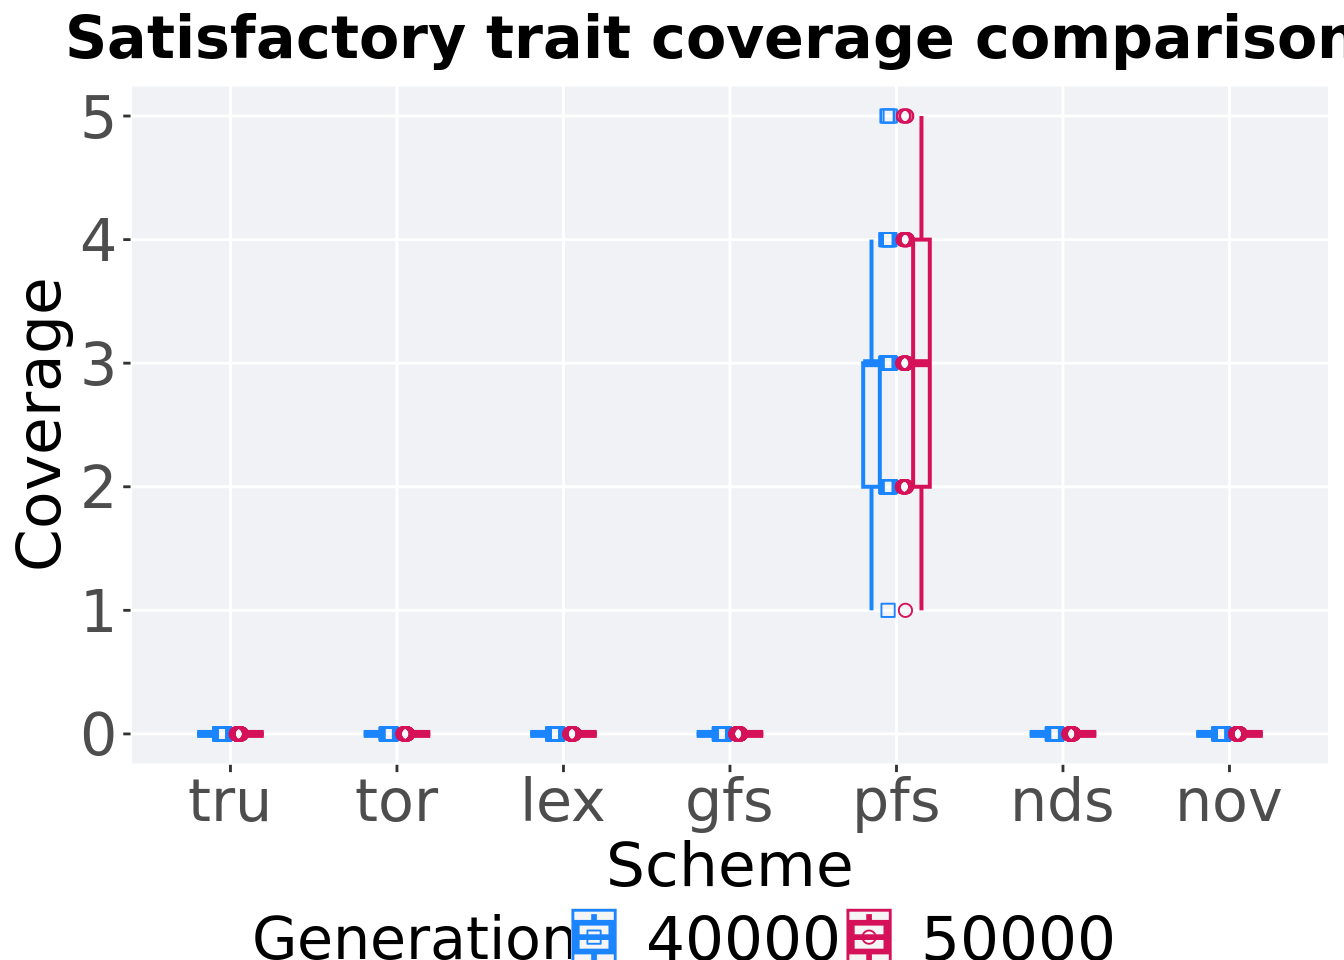
\includegraphics{demo_files/figure-latex/con-mvc-sat-sli-1.pdf}

\hypertarget{stats-14}{%
\paragraph{Stats}\label{stats-14}}

Summary statistics for the activation gene coverage at 40,000 and 50,000 generations.

\begin{Shaded}
\begin{Highlighting}[]
\NormalTok{slices =}\StringTok{ }\KeywordTok{filter}\NormalTok{(cc_over_time_mvc, diagnostic }\OperatorTok{==}\StringTok{ 'contradictory_objectives'} \OperatorTok{&}\StringTok{ }\NormalTok{(gen }\OperatorTok{==}\StringTok{ }\DecValTok{50000} \OperatorTok{|}\StringTok{ }\NormalTok{gen }\OperatorTok{==}\StringTok{ }\DecValTok{40000}\NormalTok{) }\OperatorTok{&}\StringTok{ }\NormalTok{acron }\OperatorTok{!=}\StringTok{ 'ran'}\NormalTok{)}
\NormalTok{slices}\OperatorTok{$}\NormalTok{Generation <-}\StringTok{ }\KeywordTok{factor}\NormalTok{(slices}\OperatorTok{$}\NormalTok{gen, }\DataTypeTok{levels =} \KeywordTok{c}\NormalTok{(}\DecValTok{50000}\NormalTok{,}\DecValTok{40000}\NormalTok{))}
\NormalTok{slices}\OperatorTok{$}\NormalTok{acron =}\StringTok{ }\KeywordTok{factor}\NormalTok{(slices}\OperatorTok{$}\NormalTok{acron, }\DataTypeTok{levels =} \KeywordTok{c}\NormalTok{(}\StringTok{'pfs'}\NormalTok{,}\StringTok{'nds'}\NormalTok{, }\StringTok{'lex'}\NormalTok{,  }\StringTok{'gfs'}\NormalTok{, }\StringTok{'tor'}\NormalTok{, }\StringTok{'tru'}\NormalTok{, }\StringTok{'nov'}\NormalTok{, }\StringTok{'ran'}\NormalTok{))}
\NormalTok{slices }\OperatorTok
\StringTok{  }\KeywordTok{group_by}\NormalTok{(acron, Generation) }\OperatorTok
\StringTok{  }\NormalTok{dplyr}\OperatorTok{::}\KeywordTok{summarise}\NormalTok{(}
    \DataTypeTok{count =} \KeywordTok{n}\NormalTok{(),}
    \DataTypeTok{na_cnt =} \KeywordTok{sum}\NormalTok{(}\KeywordTok{is.na}\NormalTok{(pop_uni_obj)),}
    \DataTypeTok{min =} \KeywordTok{min}\NormalTok{(pop_uni_obj, }\DataTypeTok{na.rm =} \OtherTok{TRUE}\NormalTok{),}
    \DataTypeTok{median =} \KeywordTok{median}\NormalTok{(pop_uni_obj, }\DataTypeTok{na.rm =} \OtherTok{TRUE}\NormalTok{),}
    \DataTypeTok{mean =} \KeywordTok{mean}\NormalTok{(pop_uni_obj, }\DataTypeTok{na.rm =} \OtherTok{TRUE}\NormalTok{),}
    \DataTypeTok{max =} \KeywordTok{max}\NormalTok{(pop_uni_obj, }\DataTypeTok{na.rm =} \OtherTok{TRUE}\NormalTok{),}
    \DataTypeTok{IQR =} \KeywordTok{IQR}\NormalTok{(pop_uni_obj, }\DataTypeTok{na.rm =} \OtherTok{TRUE}\NormalTok{)}
\NormalTok{  )}
\end{Highlighting}
\end{Shaded}

\begin{verbatim}
## `summarise()` has grouped output by 'acron'. You can override using the
## `.groups` argument.
\end{verbatim}

\begin{verbatim}
## # A tibble: 14 x 9
## # Groups:   acron [7]
##    acron Generation count na_cnt   min median  mean   max   IQR
##    <fct> <fct>      <int>  <int> <int>  <dbl> <dbl> <int> <dbl>
##  1 pfs   50000         50      0     1      3  3.14     5     2
##  2 pfs   40000         50      0     1      3  2.9      5     1
##  3 nds   50000         50      0     0      0  0        0     0
##  4 nds   40000         50      0     0      0  0        0     0
##  5 lex   50000         50      0     0      0  0        0     0
##  6 lex   40000         50      0     0      0  0        0     0
##  7 gfs   50000         50      0     0      0  0        0     0
##  8 gfs   40000         50      0     0      0  0        0     0
##  9 tor   50000         50      0     0      0  0        0     0
## 10 tor   40000         50      0     0      0  0        0     0
## 11 tru   50000         50      0     0      0  0        0     0
## 12 tru   40000         50      0     0      0  0        0     0
## 13 nov   50000         50      0     0      0  0        0     0
## 14 nov   40000         50      0     0      0  0        0     0
\end{verbatim}

Truncation selection comparisons.

\begin{Shaded}
\begin{Highlighting}[]
\KeywordTok{wilcox.test}\NormalTok{(}\DataTypeTok{x =} \KeywordTok{filter}\NormalTok{(slices, acron }\OperatorTok{==}\StringTok{ 'tru'} \OperatorTok{&}\StringTok{ }\NormalTok{Generation }\OperatorTok{==}\StringTok{ }\DecValTok{50000}\NormalTok{)}\OperatorTok{$}\NormalTok{pop_uni_obj,}
            \DataTypeTok{y =} \KeywordTok{filter}\NormalTok{(slices, acron }\OperatorTok{==}\StringTok{ 'tru'} \OperatorTok{&}\StringTok{ }\NormalTok{Generation }\OperatorTok{==}\StringTok{ }\DecValTok{40000}\NormalTok{)}\OperatorTok{$}\NormalTok{pop_uni_obj,}
            \DataTypeTok{alternative =} \StringTok{'t'}\NormalTok{)}
\end{Highlighting}
\end{Shaded}

\begin{verbatim}
## 
##  Wilcoxon rank sum test with continuity correction
## 
## data:  filter(slices, acron == "tru" & Generation == 50000)$pop_uni_obj and filter(slices, acron == "tru" & Generation == 40000)$pop_uni_obj
## W = 1250, p-value = NA
## alternative hypothesis: true location shift is not equal to 0
\end{verbatim}

Tournament selection comparisons.

\begin{Shaded}
\begin{Highlighting}[]
\KeywordTok{wilcox.test}\NormalTok{(}\DataTypeTok{x =} \KeywordTok{filter}\NormalTok{(slices, acron }\OperatorTok{==}\StringTok{ 'tor'} \OperatorTok{&}\StringTok{ }\NormalTok{Generation }\OperatorTok{==}\StringTok{ }\DecValTok{50000}\NormalTok{)}\OperatorTok{$}\NormalTok{pop_uni_obj,}
            \DataTypeTok{y =} \KeywordTok{filter}\NormalTok{(slices, acron }\OperatorTok{==}\StringTok{ 'tor'} \OperatorTok{&}\StringTok{ }\NormalTok{Generation }\OperatorTok{==}\StringTok{ }\DecValTok{40000}\NormalTok{)}\OperatorTok{$}\NormalTok{pop_uni_obj,}
            \DataTypeTok{alternative =} \StringTok{'t'}\NormalTok{)}
\end{Highlighting}
\end{Shaded}

\begin{verbatim}
## 
##  Wilcoxon rank sum test with continuity correction
## 
## data:  filter(slices, acron == "tor" & Generation == 50000)$pop_uni_obj and filter(slices, acron == "tor" & Generation == 40000)$pop_uni_obj
## W = 1250, p-value = NA
## alternative hypothesis: true location shift is not equal to 0
\end{verbatim}

Lexicase selection comparisons.

\begin{Shaded}
\begin{Highlighting}[]
\KeywordTok{wilcox.test}\NormalTok{(}\DataTypeTok{x =} \KeywordTok{filter}\NormalTok{(slices, acron }\OperatorTok{==}\StringTok{ 'lex'} \OperatorTok{&}\StringTok{ }\NormalTok{Generation }\OperatorTok{==}\StringTok{ }\DecValTok{50000}\NormalTok{)}\OperatorTok{$}\NormalTok{pop_uni_obj,}
            \DataTypeTok{y =} \KeywordTok{filter}\NormalTok{(slices, acron }\OperatorTok{==}\StringTok{ 'lex'} \OperatorTok{&}\StringTok{ }\NormalTok{Generation }\OperatorTok{==}\StringTok{ }\DecValTok{40000}\NormalTok{)}\OperatorTok{$}\NormalTok{pop_uni_obj,}
            \DataTypeTok{alternative =} \StringTok{'t'}\NormalTok{)}
\end{Highlighting}
\end{Shaded}

\begin{verbatim}
## 
##  Wilcoxon rank sum test with continuity correction
## 
## data:  filter(slices, acron == "lex" & Generation == 50000)$pop_uni_obj and filter(slices, acron == "lex" & Generation == 40000)$pop_uni_obj
## W = 1250, p-value = NA
## alternative hypothesis: true location shift is not equal to 0
\end{verbatim}

Genotypic fitness sharing comparisons.

\begin{Shaded}
\begin{Highlighting}[]
\KeywordTok{wilcox.test}\NormalTok{(}\DataTypeTok{x =} \KeywordTok{filter}\NormalTok{(slices, acron }\OperatorTok{==}\StringTok{ 'gfs'} \OperatorTok{&}\StringTok{ }\NormalTok{Generation }\OperatorTok{==}\StringTok{ }\DecValTok{50000}\NormalTok{)}\OperatorTok{$}\NormalTok{pop_uni_obj,}
            \DataTypeTok{y =} \KeywordTok{filter}\NormalTok{(slices, acron }\OperatorTok{==}\StringTok{ 'gfs'} \OperatorTok{&}\StringTok{ }\NormalTok{Generation }\OperatorTok{==}\StringTok{ }\DecValTok{40000}\NormalTok{)}\OperatorTok{$}\NormalTok{pop_uni_obj,}
            \DataTypeTok{alternative =} \StringTok{'t'}\NormalTok{)}
\end{Highlighting}
\end{Shaded}

\begin{verbatim}
## 
##  Wilcoxon rank sum test with continuity correction
## 
## data:  filter(slices, acron == "gfs" & Generation == 50000)$pop_uni_obj and filter(slices, acron == "gfs" & Generation == 40000)$pop_uni_obj
## W = 1250, p-value = NA
## alternative hypothesis: true location shift is not equal to 0
\end{verbatim}

Phenotypic fitness sharing comparisons.

\begin{Shaded}
\begin{Highlighting}[]
\KeywordTok{wilcox.test}\NormalTok{(}\DataTypeTok{x =} \KeywordTok{filter}\NormalTok{(slices, acron }\OperatorTok{==}\StringTok{ 'pfs'} \OperatorTok{&}\StringTok{ }\NormalTok{Generation }\OperatorTok{==}\StringTok{ }\DecValTok{50000}\NormalTok{)}\OperatorTok{$}\NormalTok{pop_uni_obj,}
            \DataTypeTok{y =} \KeywordTok{filter}\NormalTok{(slices, acron }\OperatorTok{==}\StringTok{ 'pfs'} \OperatorTok{&}\StringTok{ }\NormalTok{Generation }\OperatorTok{==}\StringTok{ }\DecValTok{40000}\NormalTok{)}\OperatorTok{$}\NormalTok{pop_uni_obj,}
            \DataTypeTok{alternative =} \StringTok{'t'}\NormalTok{)}
\end{Highlighting}
\end{Shaded}

\begin{verbatim}
## 
##  Wilcoxon rank sum test with continuity correction
## 
## data:  filter(slices, acron == "pfs" & Generation == 50000)$pop_uni_obj and filter(slices, acron == "pfs" & Generation == 40000)$pop_uni_obj
## W = 1423.5, p-value = 0.2118
## alternative hypothesis: true location shift is not equal to 0
\end{verbatim}

Nondominated sorting comparisons.

\begin{Shaded}
\begin{Highlighting}[]
\KeywordTok{wilcox.test}\NormalTok{(}\DataTypeTok{x =} \KeywordTok{filter}\NormalTok{(slices, acron }\OperatorTok{==}\StringTok{ 'nds'} \OperatorTok{&}\StringTok{ }\NormalTok{Generation }\OperatorTok{==}\StringTok{ }\DecValTok{50000}\NormalTok{)}\OperatorTok{$}\NormalTok{pop_uni_obj,}
            \DataTypeTok{y =} \KeywordTok{filter}\NormalTok{(slices, acron }\OperatorTok{==}\StringTok{ 'nds'} \OperatorTok{&}\StringTok{ }\NormalTok{Generation }\OperatorTok{==}\StringTok{ }\DecValTok{40000}\NormalTok{)}\OperatorTok{$}\NormalTok{pop_uni_obj,}
            \DataTypeTok{alternative =} \StringTok{'t'}\NormalTok{)}
\end{Highlighting}
\end{Shaded}

\begin{verbatim}
## 
##  Wilcoxon rank sum test with continuity correction
## 
## data:  filter(slices, acron == "nds" & Generation == 50000)$pop_uni_obj and filter(slices, acron == "nds" & Generation == 40000)$pop_uni_obj
## W = 1250, p-value = NA
## alternative hypothesis: true location shift is not equal to 0
\end{verbatim}

Novelty search comparisons.

\begin{Shaded}
\begin{Highlighting}[]
\KeywordTok{wilcox.test}\NormalTok{(}\DataTypeTok{x =} \KeywordTok{filter}\NormalTok{(slices, acron }\OperatorTok{==}\StringTok{ 'nov'} \OperatorTok{&}\StringTok{ }\NormalTok{Generation }\OperatorTok{==}\StringTok{ }\DecValTok{50000}\NormalTok{)}\OperatorTok{$}\NormalTok{pop_uni_obj,}
            \DataTypeTok{y =} \KeywordTok{filter}\NormalTok{(slices, acron }\OperatorTok{==}\StringTok{ 'nov'} \OperatorTok{&}\StringTok{ }\NormalTok{Generation }\OperatorTok{==}\StringTok{ }\DecValTok{40000}\NormalTok{)}\OperatorTok{$}\NormalTok{pop_uni_obj,}
            \DataTypeTok{alternative =} \StringTok{'t'}\NormalTok{)}
\end{Highlighting}
\end{Shaded}

\begin{verbatim}
## 
##  Wilcoxon rank sum test with continuity correction
## 
## data:  filter(slices, acron == "nov" & Generation == 50000)$pop_uni_obj and filter(slices, acron == "nov" & Generation == 40000)$pop_uni_obj
## W = 1250, p-value = NA
## alternative hypothesis: true location shift is not equal to 0
\end{verbatim}

\hypertarget{activation-gene-coverage-1}{%
\subsection{Activation gene coverage}\label{activation-gene-coverage-1}}

Activation gene coverage analysis.

\hypertarget{coverage-over-time-3}{%
\subsubsection{Coverage over time}\label{coverage-over-time-3}}

Activation gene coverage over time.

\begin{Shaded}
\begin{Highlighting}[]
\NormalTok{lines =}\StringTok{ }\KeywordTok{filter}\NormalTok{(cc_over_time_mvc, diagnostic }\OperatorTok{==}\StringTok{ 'contradictory_objectives'}\NormalTok{) }\OperatorTok
\StringTok{  }\KeywordTok{group_by}\NormalTok{(}\StringTok{`}\DataTypeTok{Selection}\CharTok{\textbackslash{}n}\DataTypeTok{Scheme}\StringTok{`}\NormalTok{, gen) }\OperatorTok
\StringTok{  }\NormalTok{dplyr}\OperatorTok{::}\KeywordTok{summarise}\NormalTok{(}
    \DataTypeTok{min =} \KeywordTok{min}\NormalTok{(uni_str_pos),}
    \DataTypeTok{mean =} \KeywordTok{mean}\NormalTok{(uni_str_pos),}
    \DataTypeTok{max =} \KeywordTok{max}\NormalTok{(uni_str_pos)}
\NormalTok{  )}
\end{Highlighting}
\end{Shaded}

\begin{verbatim}
## `summarise()` has grouped output by 'Selection Scheme'. You can override using
## the `.groups` argument.
\end{verbatim}

\begin{Shaded}
\begin{Highlighting}[]
\KeywordTok{ggplot}\NormalTok{(lines, }\KeywordTok{aes}\NormalTok{(}\DataTypeTok{x=}\NormalTok{gen, }\DataTypeTok{y=}\NormalTok{mean, }\DataTypeTok{group =} \StringTok{`}\DataTypeTok{Selection}\CharTok{\textbackslash{}n}\DataTypeTok{Scheme}\StringTok{`}\NormalTok{, }\DataTypeTok{fill =}\StringTok{`}\DataTypeTok{Selection}\CharTok{\textbackslash{}n}\DataTypeTok{Scheme}\StringTok{`}\NormalTok{, }\DataTypeTok{color =} \StringTok{`}\DataTypeTok{Selection}\CharTok{\textbackslash{}n}\DataTypeTok{Scheme}\StringTok{`}\NormalTok{, }\DataTypeTok{shape =} \StringTok{`}\DataTypeTok{Selection}\CharTok{\textbackslash{}n}\DataTypeTok{Scheme}\StringTok{`}\NormalTok{)) }\OperatorTok{+}
\StringTok{  }\KeywordTok{geom_ribbon}\NormalTok{(}\KeywordTok{aes}\NormalTok{(}\DataTypeTok{ymin =}\NormalTok{ min, }\DataTypeTok{ymax =}\NormalTok{ max), }\DataTypeTok{alpha =} \FloatTok{0.1}\NormalTok{) }\OperatorTok{+}
\StringTok{  }\KeywordTok{geom_line}\NormalTok{(}\DataTypeTok{size =} \FloatTok{0.5}\NormalTok{) }\OperatorTok{+}
\StringTok{  }\KeywordTok{geom_point}\NormalTok{(}\DataTypeTok{data =} \KeywordTok{filter}\NormalTok{(lines, gen }\OperatorTok\StringTok{ }\DecValTok{2000} \OperatorTok{==}\StringTok{ }\DecValTok{0} \OperatorTok{&}\StringTok{ }\NormalTok{gen }\OperatorTok{!=}\StringTok{ }\DecValTok{0}\NormalTok{), }\DataTypeTok{size =} \FloatTok{1.5}\NormalTok{, }\DataTypeTok{stroke =} \FloatTok{2.0}\NormalTok{, }\DataTypeTok{alpha =} \FloatTok{1.0}\NormalTok{) }\OperatorTok{+}
\StringTok{  }\KeywordTok{scale_y_continuous}\NormalTok{(}
    \DataTypeTok{name=}\StringTok{"Coverage"}\NormalTok{,}
    \DataTypeTok{limits=}\KeywordTok{c}\NormalTok{(}\DecValTok{0}\NormalTok{, }\DecValTok{100}\NormalTok{),}
    \DataTypeTok{breaks=}\KeywordTok{seq}\NormalTok{(}\DecValTok{0}\NormalTok{,}\DecValTok{100}\NormalTok{, }\DecValTok{20}\NormalTok{),}
    \DataTypeTok{labels=}\KeywordTok{c}\NormalTok{(}\StringTok{"0"}\NormalTok{, }\StringTok{"20"}\NormalTok{, }\StringTok{"40"}\NormalTok{, }\StringTok{"60"}\NormalTok{, }\StringTok{"80"}\NormalTok{, }\StringTok{"100"}\NormalTok{)}
\NormalTok{  ) }\OperatorTok{+}
\StringTok{  }\KeywordTok{scale_x_continuous}\NormalTok{(}
    \DataTypeTok{name=}\StringTok{"Generations"}\NormalTok{,}
    \DataTypeTok{limits=}\KeywordTok{c}\NormalTok{(}\DecValTok{0}\NormalTok{, }\DecValTok{50000}\NormalTok{),}
    \DataTypeTok{breaks=}\KeywordTok{c}\NormalTok{(}\DecValTok{0}\NormalTok{, }\DecValTok{10000}\NormalTok{, }\DecValTok{20000}\NormalTok{, }\DecValTok{30000}\NormalTok{, }\DecValTok{40000}\NormalTok{, }\DecValTok{50000}\NormalTok{),}
    \DataTypeTok{labels=}\KeywordTok{c}\NormalTok{(}\StringTok{"0e+4"}\NormalTok{, }\StringTok{"1e+4"}\NormalTok{, }\StringTok{"2e+4"}\NormalTok{, }\StringTok{"3e+4"}\NormalTok{, }\StringTok{"4e+4"}\NormalTok{, }\StringTok{"5e+4"}\NormalTok{)}
\NormalTok{  ) }\OperatorTok{+}
\StringTok{  }\KeywordTok{scale_shape_manual}\NormalTok{(}\DataTypeTok{values=}\NormalTok{SHAPE)}\OperatorTok{+}
\StringTok{  }\KeywordTok{scale_colour_manual}\NormalTok{(}\DataTypeTok{values =}\NormalTok{ cb_palette) }\OperatorTok{+}
\StringTok{  }\KeywordTok{scale_fill_manual}\NormalTok{(}\DataTypeTok{values =}\NormalTok{ cb_palette) }\OperatorTok{+}
\StringTok{  }\KeywordTok{ggtitle}\NormalTok{(}\StringTok{'Activation gene coverage over time'}\NormalTok{)}\OperatorTok{+}
\StringTok{  }\NormalTok{p_theme }\OperatorTok{+}\StringTok{ }\KeywordTok{theme}\NormalTok{(}\DataTypeTok{legend.title=}\KeywordTok{element_blank}\NormalTok{(),}\DataTypeTok{legend.text=}\KeywordTok{element_text}\NormalTok{(}\DataTypeTok{size=}\DecValTok{11}\NormalTok{)) }\OperatorTok{+}
\StringTok{  }\KeywordTok{guides}\NormalTok{(}
    \DataTypeTok{shape=}\KeywordTok{guide_legend}\NormalTok{(}\DataTypeTok{ncol=}\DecValTok{2}\NormalTok{, }\DataTypeTok{title.position =} \StringTok{"bottom"}\NormalTok{),}
    \DataTypeTok{color=}\KeywordTok{guide_legend}\NormalTok{(}\DataTypeTok{ncol=}\DecValTok{2}\NormalTok{, }\DataTypeTok{title.position =} \StringTok{"bottom"}\NormalTok{),}
    \DataTypeTok{fill=}\KeywordTok{guide_legend}\NormalTok{(}\DataTypeTok{ncol=}\DecValTok{2}\NormalTok{, }\DataTypeTok{title.position =} \StringTok{"bottom"}\NormalTok{)}
\NormalTok{  )}
\end{Highlighting}
\end{Shaded}

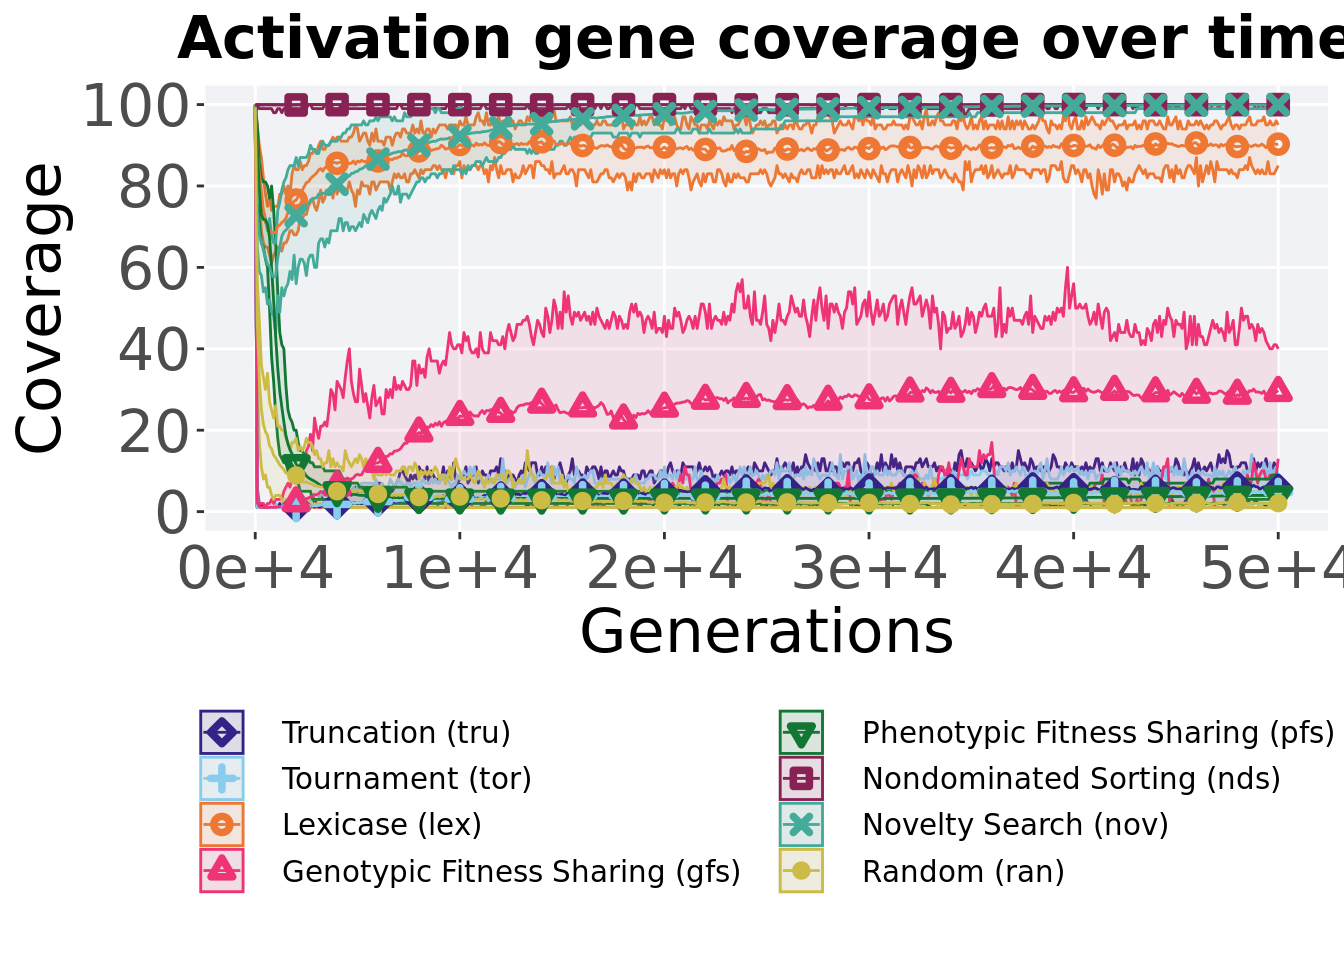
\includegraphics{demo_files/figure-latex/con-mvc-act-ot-1.pdf}

\hypertarget{coverage-comparison-1}{%
\subsubsection{Coverage comparison}\label{coverage-comparison-1}}

Best activation gene coverage in the population at 40,000 and 50,000 generations.

\begin{Shaded}
\begin{Highlighting}[]
\NormalTok{mvc_p =}\StringTok{ }\KeywordTok{ggplot}\NormalTok{(mid, }\KeywordTok{aes}\NormalTok{(}\DataTypeTok{x =}\NormalTok{ acron, }\DataTypeTok{y=}\NormalTok{uni_str_pos, }\DataTypeTok{group =}\NormalTok{ acron, }\DataTypeTok{shape =}\NormalTok{ Generation)) }\OperatorTok{+}
\StringTok{  }\KeywordTok{geom_point}\NormalTok{(}\DataTypeTok{col =}\NormalTok{ mvc_col[}\DecValTok{1}\NormalTok{] , }\DataTypeTok{position =} \KeywordTok{position_jitternudge}\NormalTok{(}\DataTypeTok{jitter.width =} \FloatTok{.03}\NormalTok{, }\DataTypeTok{nudge.x =} \FloatTok{-0.05}\NormalTok{), }\DataTypeTok{size =} \DecValTok{2}\NormalTok{, }\DataTypeTok{alpha =} \FloatTok{1.0}\NormalTok{) }\OperatorTok{+}
\StringTok{  }\KeywordTok{geom_boxplot}\NormalTok{(}\DataTypeTok{position =} \KeywordTok{position_nudge}\NormalTok{(}\DataTypeTok{x =} \FloatTok{-.15}\NormalTok{, }\DataTypeTok{y =} \DecValTok{0}\NormalTok{), }\DataTypeTok{lwd =} \FloatTok{0.7}\NormalTok{, }\DataTypeTok{col =}\NormalTok{ mvc_col[}\DecValTok{1}\NormalTok{], }\DataTypeTok{fill =}\NormalTok{ mvc_col[}\DecValTok{1}\NormalTok{], }\DataTypeTok{width =} \FloatTok{.1}\NormalTok{, }\DataTypeTok{outlier.shape =} \OtherTok{NA}\NormalTok{, }\DataTypeTok{alpha =} \FloatTok{0.0}\NormalTok{) }\OperatorTok{+}

\StringTok{  }\KeywordTok{geom_point}\NormalTok{(}\DataTypeTok{data =}\NormalTok{ end, }\KeywordTok{aes}\NormalTok{(}\DataTypeTok{x =}\NormalTok{ acron, }\DataTypeTok{y=}\NormalTok{uni_str_pos), }\DataTypeTok{col =}\NormalTok{ mvc_col[}\DecValTok{2}\NormalTok{], }\DataTypeTok{position =} \KeywordTok{position_jitternudge}\NormalTok{(}\DataTypeTok{jitter.width =} \FloatTok{.03}\NormalTok{, }\DataTypeTok{nudge.x =} \FloatTok{0.05}\NormalTok{), }\DataTypeTok{size =} \DecValTok{2}\NormalTok{, }\DataTypeTok{alpha =} \FloatTok{1.0}\NormalTok{) }\OperatorTok{+}
\StringTok{  }\KeywordTok{geom_boxplot}\NormalTok{(}\DataTypeTok{data =}\NormalTok{ end, }\KeywordTok{aes}\NormalTok{(}\DataTypeTok{x =}\NormalTok{ acron, }\DataTypeTok{y=}\NormalTok{uni_str_pos), }\DataTypeTok{position =} \KeywordTok{position_nudge}\NormalTok{(}\DataTypeTok{x =} \FloatTok{.15}\NormalTok{, }\DataTypeTok{y =} \DecValTok{0}\NormalTok{), }\DataTypeTok{lwd =} \FloatTok{0.7}\NormalTok{, }\DataTypeTok{col =}\NormalTok{ mvc_col[}\DecValTok{2}\NormalTok{], }\DataTypeTok{fill =}\NormalTok{ mvc_col[}\DecValTok{2}\NormalTok{], }\DataTypeTok{width =} \FloatTok{.1}\NormalTok{, }\DataTypeTok{outlier.shape =} \OtherTok{NA}\NormalTok{, }\DataTypeTok{alpha =} \FloatTok{0.0}\NormalTok{) }\OperatorTok{+}

\StringTok{  }\KeywordTok{scale_y_continuous}\NormalTok{(}
    \DataTypeTok{name=}\StringTok{"Coverage"}\NormalTok{,}
    \DataTypeTok{limits=}\KeywordTok{c}\NormalTok{(}\DecValTok{0}\NormalTok{, }\DecValTok{100}\NormalTok{),}
    \DataTypeTok{breaks=}\KeywordTok{seq}\NormalTok{(}\DecValTok{0}\NormalTok{,}\DecValTok{100}\NormalTok{, }\DecValTok{20}\NormalTok{),}
    \DataTypeTok{labels=}\KeywordTok{c}\NormalTok{(}\StringTok{"0"}\NormalTok{, }\StringTok{"20"}\NormalTok{, }\StringTok{"40"}\NormalTok{, }\StringTok{"60"}\NormalTok{, }\StringTok{"80"}\NormalTok{, }\StringTok{"100"}\NormalTok{)  ) }\OperatorTok{+}
\StringTok{  }\KeywordTok{scale_x_discrete}\NormalTok{(}
    \DataTypeTok{name=}\StringTok{"Scheme"}
\NormalTok{  )}\OperatorTok{+}
\StringTok{  }\KeywordTok{scale_shape_manual}\NormalTok{(}\DataTypeTok{values=}\KeywordTok{c}\NormalTok{(}\DecValTok{0}\NormalTok{,}\DecValTok{1}\NormalTok{))}\OperatorTok{+}
\StringTok{  }\KeywordTok{scale_colour_manual}\NormalTok{(}\DataTypeTok{values =} \KeywordTok{c}\NormalTok{(mvc_col[}\DecValTok{1}\NormalTok{],mvc_col[}\DecValTok{2}\NormalTok{])) }\OperatorTok{+}
\StringTok{  }\NormalTok{p_theme}

\KeywordTok{plot_grid}\NormalTok{(}
\NormalTok{  mvc_p }\OperatorTok{+}
\StringTok{    }\KeywordTok{ggtitle}\NormalTok{(}\StringTok{"Activation gene coverage comparisons"}\NormalTok{) }\OperatorTok{+}
\StringTok{    }\KeywordTok{theme}\NormalTok{(}\DataTypeTok{legend.position=}\StringTok{"none"}\NormalTok{),}
\NormalTok{  legend,}
  \DataTypeTok{nrow=}\DecValTok{2}\NormalTok{,}
  \DataTypeTok{rel_heights =} \KeywordTok{c}\NormalTok{(}\DecValTok{1}\NormalTok{,.}\DecValTok{05}\NormalTok{),}
  \DataTypeTok{label_size =}\NormalTok{ TSIZE}
\NormalTok{)}
\end{Highlighting}
\end{Shaded}

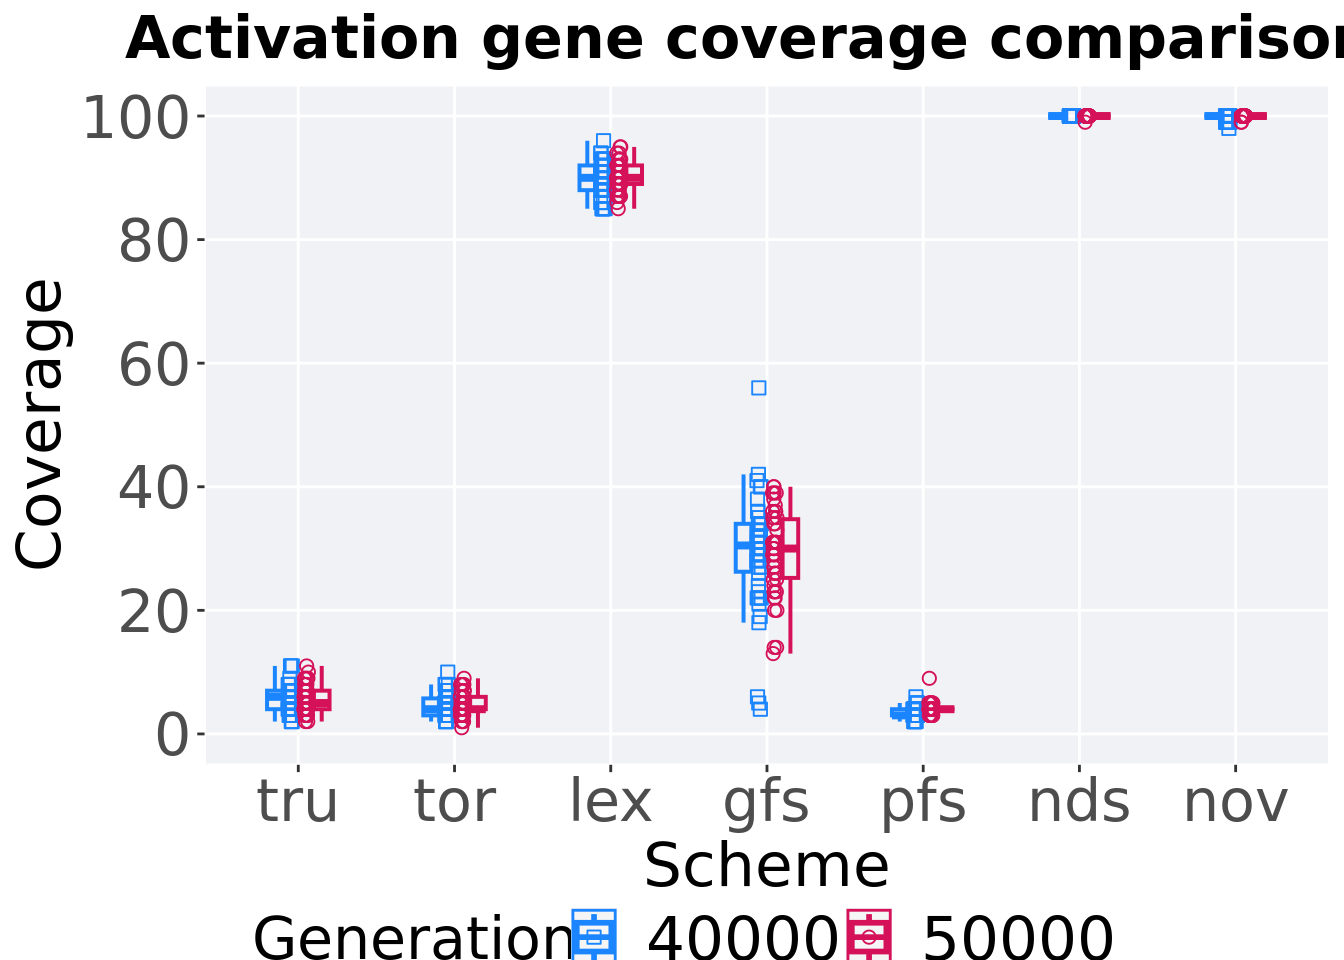
\includegraphics{demo_files/figure-latex/con-mvc-act-sli-1.pdf}

\hypertarget{stats-15}{%
\subsubsection{Stats}\label{stats-15}}

Summary statistics for the activation gene coverage at 40,000 and 50,000 generations.

\begin{Shaded}
\begin{Highlighting}[]
\NormalTok{slices =}\StringTok{ }\KeywordTok{filter}\NormalTok{(cc_over_time_mvc, diagnostic }\OperatorTok{==}\StringTok{ 'contradictory_objectives'} \OperatorTok{&}\StringTok{ }\NormalTok{(gen }\OperatorTok{==}\StringTok{ }\DecValTok{50000} \OperatorTok{|}\StringTok{ }\NormalTok{gen }\OperatorTok{==}\StringTok{ }\DecValTok{40000}\NormalTok{) }\OperatorTok{&}\StringTok{ }\NormalTok{acron }\OperatorTok{!=}\StringTok{ 'ran'}\NormalTok{)}
\NormalTok{slices}\OperatorTok{$}\NormalTok{Generation <-}\StringTok{ }\KeywordTok{factor}\NormalTok{(slices}\OperatorTok{$}\NormalTok{gen, }\DataTypeTok{levels =} \KeywordTok{c}\NormalTok{(}\DecValTok{50000}\NormalTok{,}\DecValTok{40000}\NormalTok{))}
\NormalTok{slices}\OperatorTok{$}\NormalTok{acron =}\StringTok{ }\KeywordTok{factor}\NormalTok{(slices}\OperatorTok{$}\NormalTok{acron, }\DataTypeTok{levels =} \KeywordTok{c}\NormalTok{(}\StringTok{'nov'}\NormalTok{,}\StringTok{'nds'}\NormalTok{,}\StringTok{'lex'}\NormalTok{,}\StringTok{'gfs'}\NormalTok{,}\StringTok{'tor'}\NormalTok{,}\StringTok{'tru'}\NormalTok{,}\StringTok{'pfs'}\NormalTok{))}
\NormalTok{slices }\OperatorTok
\StringTok{  }\KeywordTok{group_by}\NormalTok{(acron, Generation) }\OperatorTok
\StringTok{  }\NormalTok{dplyr}\OperatorTok{::}\KeywordTok{summarise}\NormalTok{(}
    \DataTypeTok{count =} \KeywordTok{n}\NormalTok{(),}
    \DataTypeTok{na_cnt =} \KeywordTok{sum}\NormalTok{(}\KeywordTok{is.na}\NormalTok{(uni_str_pos)),}
    \DataTypeTok{min =} \KeywordTok{min}\NormalTok{(uni_str_pos, }\DataTypeTok{na.rm =} \OtherTok{TRUE}\NormalTok{),}
    \DataTypeTok{median =} \KeywordTok{median}\NormalTok{(uni_str_pos, }\DataTypeTok{na.rm =} \OtherTok{TRUE}\NormalTok{),}
    \DataTypeTok{mean =} \KeywordTok{mean}\NormalTok{(uni_str_pos, }\DataTypeTok{na.rm =} \OtherTok{TRUE}\NormalTok{),}
    \DataTypeTok{max =} \KeywordTok{max}\NormalTok{(uni_str_pos, }\DataTypeTok{na.rm =} \OtherTok{TRUE}\NormalTok{),}
    \DataTypeTok{IQR =} \KeywordTok{IQR}\NormalTok{(uni_str_pos, }\DataTypeTok{na.rm =} \OtherTok{TRUE}\NormalTok{)}
\NormalTok{  )}
\end{Highlighting}
\end{Shaded}

\begin{verbatim}
## `summarise()` has grouped output by 'acron'. You can override using the
## `.groups` argument.
\end{verbatim}

\begin{verbatim}
## # A tibble: 14 x 9
## # Groups:   acron [7]
##    acron Generation count na_cnt   min median   mean   max   IQR
##    <fct> <fct>      <int>  <int> <int>  <dbl>  <dbl> <int> <dbl>
##  1 nov   50000         50      0    99  100   100.     100  0   
##  2 nov   40000         50      0    98  100    99.8    100  0   
##  3 nds   50000         50      0    99  100   100.     100  0   
##  4 nds   40000         50      0   100  100   100      100  0   
##  5 lex   50000         50      0    85   90    90.3     95  3   
##  6 lex   40000         50      0    85   90    90.0     96  4   
##  7 gfs   50000         50      0    13   30    29.4     40  9.5 
##  8 gfs   40000         50      0     4   30.5  29.3     56  7.75
##  9 tor   50000         50      0     1    4     4.64     9  2   
## 10 tor   40000         50      0     2    4     4.54    10  2.75
## 11 tru   50000         50      0     2    5     5.6     11  3   
## 12 tru   40000         50      0     2    6     5.8     11  3   
## 13 pfs   50000         50      0     3    4     4.02     9  0   
## 14 pfs   40000         50      0     2    3     3.42     6  1
\end{verbatim}

Truncation selection comparisons.

\begin{Shaded}
\begin{Highlighting}[]
\KeywordTok{wilcox.test}\NormalTok{(}\DataTypeTok{x =} \KeywordTok{filter}\NormalTok{(slices, acron }\OperatorTok{==}\StringTok{ 'tru'} \OperatorTok{&}\StringTok{ }\NormalTok{Generation }\OperatorTok{==}\StringTok{ }\DecValTok{50000}\NormalTok{)}\OperatorTok{$}\NormalTok{uni_str_pos,}
            \DataTypeTok{y =} \KeywordTok{filter}\NormalTok{(slices, acron }\OperatorTok{==}\StringTok{ 'tru'} \OperatorTok{&}\StringTok{ }\NormalTok{Generation }\OperatorTok{==}\StringTok{ }\DecValTok{40000}\NormalTok{)}\OperatorTok{$}\NormalTok{uni_str_pos,}
            \DataTypeTok{alternative =} \StringTok{'t'}\NormalTok{)}
\end{Highlighting}
\end{Shaded}

\begin{verbatim}
## 
##  Wilcoxon rank sum test with continuity correction
## 
## data:  filter(slices, acron == "tru" & Generation == 50000)$uni_str_pos and filter(slices, acron == "tru" & Generation == 40000)$uni_str_pos
## W = 1175, p-value = 0.6039
## alternative hypothesis: true location shift is not equal to 0
\end{verbatim}

Tournament selection comparisons.

\begin{Shaded}
\begin{Highlighting}[]
\KeywordTok{wilcox.test}\NormalTok{(}\DataTypeTok{x =} \KeywordTok{filter}\NormalTok{(slices, acron }\OperatorTok{==}\StringTok{ 'tor'} \OperatorTok{&}\StringTok{ }\NormalTok{Generation }\OperatorTok{==}\StringTok{ }\DecValTok{50000}\NormalTok{)}\OperatorTok{$}\NormalTok{uni_str_pos,}
            \DataTypeTok{y =} \KeywordTok{filter}\NormalTok{(slices, acron }\OperatorTok{==}\StringTok{ 'tor'} \OperatorTok{&}\StringTok{ }\NormalTok{Generation }\OperatorTok{==}\StringTok{ }\DecValTok{40000}\NormalTok{)}\OperatorTok{$}\NormalTok{uni_str_pos,}
            \DataTypeTok{alternative =} \StringTok{'t'}\NormalTok{)}
\end{Highlighting}
\end{Shaded}

\begin{verbatim}
## 
##  Wilcoxon rank sum test with continuity correction
## 
## data:  filter(slices, acron == "tor" & Generation == 50000)$uni_str_pos and filter(slices, acron == "tor" & Generation == 40000)$uni_str_pos
## W = 1351.5, p-value = 0.4781
## alternative hypothesis: true location shift is not equal to 0
\end{verbatim}

Lexicase selection comparisons.

\begin{Shaded}
\begin{Highlighting}[]
\KeywordTok{wilcox.test}\NormalTok{(}\DataTypeTok{x =} \KeywordTok{filter}\NormalTok{(slices, acron }\OperatorTok{==}\StringTok{ 'lex'} \OperatorTok{&}\StringTok{ }\NormalTok{Generation }\OperatorTok{==}\StringTok{ }\DecValTok{50000}\NormalTok{)}\OperatorTok{$}\NormalTok{uni_str_pos,}
            \DataTypeTok{y =} \KeywordTok{filter}\NormalTok{(slices, acron }\OperatorTok{==}\StringTok{ 'lex'} \OperatorTok{&}\StringTok{ }\NormalTok{Generation }\OperatorTok{==}\StringTok{ }\DecValTok{40000}\NormalTok{)}\OperatorTok{$}\NormalTok{uni_str_pos,}
            \DataTypeTok{alternative =} \StringTok{'t'}\NormalTok{)}
\end{Highlighting}
\end{Shaded}

\begin{verbatim}
## 
##  Wilcoxon rank sum test with continuity correction
## 
## data:  filter(slices, acron == "lex" & Generation == 50000)$uni_str_pos and filter(slices, acron == "lex" & Generation == 40000)$uni_str_pos
## W = 1321.5, p-value = 0.6221
## alternative hypothesis: true location shift is not equal to 0
\end{verbatim}

Genotypic fitness sharing comparisons.

\begin{Shaded}
\begin{Highlighting}[]
\KeywordTok{wilcox.test}\NormalTok{(}\DataTypeTok{x =} \KeywordTok{filter}\NormalTok{(slices, acron }\OperatorTok{==}\StringTok{ 'gfs'} \OperatorTok{&}\StringTok{ }\NormalTok{Generation }\OperatorTok{==}\StringTok{ }\DecValTok{50000}\NormalTok{)}\OperatorTok{$}\NormalTok{uni_str_pos,}
            \DataTypeTok{y =} \KeywordTok{filter}\NormalTok{(slices, acron }\OperatorTok{==}\StringTok{ 'gfs'} \OperatorTok{&}\StringTok{ }\NormalTok{Generation }\OperatorTok{==}\StringTok{ }\DecValTok{40000}\NormalTok{)}\OperatorTok{$}\NormalTok{uni_str_pos,}
            \DataTypeTok{alternative =} \StringTok{'t'}\NormalTok{)}
\end{Highlighting}
\end{Shaded}

\begin{verbatim}
## 
##  Wilcoxon rank sum test with continuity correction
## 
## data:  filter(slices, acron == "gfs" & Generation == 50000)$uni_str_pos and filter(slices, acron == "gfs" & Generation == 40000)$uni_str_pos
## W = 1223.5, p-value = 0.8575
## alternative hypothesis: true location shift is not equal to 0
\end{verbatim}

Phenotypic fitness sharing comparisons.

\begin{Shaded}
\begin{Highlighting}[]
\KeywordTok{wilcox.test}\NormalTok{(}\DataTypeTok{x =} \KeywordTok{filter}\NormalTok{(slices, acron }\OperatorTok{==}\StringTok{ 'pfs'} \OperatorTok{&}\StringTok{ }\NormalTok{Generation }\OperatorTok{==}\StringTok{ }\DecValTok{50000}\NormalTok{)}\OperatorTok{$}\NormalTok{uni_str_pos,}
            \DataTypeTok{y =} \KeywordTok{filter}\NormalTok{(slices, acron }\OperatorTok{==}\StringTok{ 'pfs'} \OperatorTok{&}\StringTok{ }\NormalTok{Generation }\OperatorTok{==}\StringTok{ }\DecValTok{40000}\NormalTok{)}\OperatorTok{$}\NormalTok{uni_str_pos,}
            \DataTypeTok{alternative =} \StringTok{'t'}\NormalTok{)}
\end{Highlighting}
\end{Shaded}

\begin{verbatim}
## 
##  Wilcoxon rank sum test with continuity correction
## 
## data:  filter(slices, acron == "pfs" & Generation == 50000)$uni_str_pos and filter(slices, acron == "pfs" & Generation == 40000)$uni_str_pos
## W = 1709, p-value = 0.0006733
## alternative hypothesis: true location shift is not equal to 0
\end{verbatim}

Nondominated sorting comparisons.

\begin{Shaded}
\begin{Highlighting}[]
\KeywordTok{wilcox.test}\NormalTok{(}\DataTypeTok{x =} \KeywordTok{filter}\NormalTok{(slices, acron }\OperatorTok{==}\StringTok{ 'nds'} \OperatorTok{&}\StringTok{ }\NormalTok{Generation }\OperatorTok{==}\StringTok{ }\DecValTok{50000}\NormalTok{)}\OperatorTok{$}\NormalTok{uni_str_pos,}
            \DataTypeTok{y =} \KeywordTok{filter}\NormalTok{(slices, acron }\OperatorTok{==}\StringTok{ 'nds'} \OperatorTok{&}\StringTok{ }\NormalTok{Generation }\OperatorTok{==}\StringTok{ }\DecValTok{40000}\NormalTok{)}\OperatorTok{$}\NormalTok{uni_str_pos,}
            \DataTypeTok{alternative =} \StringTok{'t'}\NormalTok{)}
\end{Highlighting}
\end{Shaded}

\begin{verbatim}
## 
##  Wilcoxon rank sum test with continuity correction
## 
## data:  filter(slices, acron == "nds" & Generation == 50000)$uni_str_pos and filter(slices, acron == "nds" & Generation == 40000)$uni_str_pos
## W = 1225, p-value = 0.3271
## alternative hypothesis: true location shift is not equal to 0
\end{verbatim}

Novelty search comparisons.

\begin{Shaded}
\begin{Highlighting}[]
\KeywordTok{wilcox.test}\NormalTok{(}\DataTypeTok{x =} \KeywordTok{filter}\NormalTok{(slices, acron }\OperatorTok{==}\StringTok{ 'nov'} \OperatorTok{&}\StringTok{ }\NormalTok{Generation }\OperatorTok{==}\StringTok{ }\DecValTok{50000}\NormalTok{)}\OperatorTok{$}\NormalTok{uni_str_pos,}
            \DataTypeTok{y =} \KeywordTok{filter}\NormalTok{(slices, acron }\OperatorTok{==}\StringTok{ 'nov'} \OperatorTok{&}\StringTok{ }\NormalTok{Generation }\OperatorTok{==}\StringTok{ }\DecValTok{40000}\NormalTok{)}\OperatorTok{$}\NormalTok{uni_str_pos,}
            \DataTypeTok{alternative =} \StringTok{'t'}\NormalTok{)}
\end{Highlighting}
\end{Shaded}

\begin{verbatim}
## 
##  Wilcoxon rank sum test with continuity correction
## 
## data:  filter(slices, acron == "nov" & Generation == 50000)$uni_str_pos and filter(slices, acron == "nov" & Generation == 40000)$uni_str_pos
## W = 1476, p-value = 0.007657
## alternative hypothesis: true location shift is not equal to 0
\end{verbatim}

\hypertarget{multi-path-mpeloration-results}{%
\chapter{Multi-path mpeloration results}\label{multi-path-mpeloration-results}}

Here we present the results for the \textbf{best performances} and \textbf{activation gene coverage} generated by each selection scheme replicate on the multi-path mpeloration diagnostic.
Best performance found refers to the largest average trait score found in a given population.
Note that activation gene coverage values are gathered at the population-level.
Activation gene coverage refers to the count of unique activation genes in a given population; this gives us a range of integers between 0 and 100.

\hypertarget{analysis-dependencies-3}{%
\section{Analysis dependencies}\label{analysis-dependencies-3}}

\begin{Shaded}
\begin{Highlighting}[]
\KeywordTok{library}\NormalTok{(ggplot2)}
\KeywordTok{library}\NormalTok{(cowplot)}
\KeywordTok{library}\NormalTok{(dplyr)}
\KeywordTok{library}\NormalTok{(PupillometryR)}
\KeywordTok{library}\NormalTok{(sdamr)}
\end{Highlighting}
\end{Shaded}

\hypertarget{performance}{%
\section{Performance}\label{performance}}

Performance analysis.

\hypertarget{over-time}{%
\subsection{Over time}\label{over-time}}

Best performance in a population over time.

\begin{Shaded}
\begin{Highlighting}[]
\CommentTok{# data for lines and shading on plots}
\NormalTok{lines =}\StringTok{ }\KeywordTok{filter}\NormalTok{(cc_over_time, diagnostic }\OperatorTok{==}\StringTok{ 'multipath_exploration'}\NormalTok{) }\OperatorTok
\StringTok{  }\KeywordTok{group_by}\NormalTok{(}\StringTok{`}\DataTypeTok{Selection}\CharTok{\textbackslash{}n}\DataTypeTok{Scheme}\StringTok{`}\NormalTok{, gen) }\OperatorTok
\StringTok{  }\NormalTok{dplyr}\OperatorTok{::}\KeywordTok{summarise}\NormalTok{(}
    \DataTypeTok{min =} \KeywordTok{min}\NormalTok{(pop_fit_max) }\OperatorTok{/}\StringTok{ }\NormalTok{DIMENSIONALITY,}
    \DataTypeTok{mean =} \KeywordTok{mean}\NormalTok{(pop_fit_max) }\OperatorTok{/}\StringTok{ }\NormalTok{DIMENSIONALITY,}
    \DataTypeTok{max =} \KeywordTok{max}\NormalTok{(pop_fit_max) }\OperatorTok{/}\StringTok{ }\NormalTok{DIMENSIONALITY}
\NormalTok{  )}
\end{Highlighting}
\end{Shaded}

\begin{verbatim}
## `summarise()` has grouped output by 'Selection Scheme'. You can override using
## the `.groups` argument.
\end{verbatim}

\begin{Shaded}
\begin{Highlighting}[]
\KeywordTok{ggplot}\NormalTok{(lines, }\KeywordTok{aes}\NormalTok{(}\DataTypeTok{x=}\NormalTok{gen, }\DataTypeTok{y=}\NormalTok{mean, }\DataTypeTok{group =} \StringTok{`}\DataTypeTok{Selection}\CharTok{\textbackslash{}n}\DataTypeTok{Scheme}\StringTok{`}\NormalTok{, }\DataTypeTok{fill =}\StringTok{`}\DataTypeTok{Selection}\CharTok{\textbackslash{}n}\DataTypeTok{Scheme}\StringTok{`}\NormalTok{, }\DataTypeTok{color =} \StringTok{`}\DataTypeTok{Selection}\CharTok{\textbackslash{}n}\DataTypeTok{Scheme}\StringTok{`}\NormalTok{, }\DataTypeTok{shape =} \StringTok{`}\DataTypeTok{Selection}\CharTok{\textbackslash{}n}\DataTypeTok{Scheme}\StringTok{`}\NormalTok{)) }\OperatorTok{+}
\StringTok{  }\KeywordTok{geom_ribbon}\NormalTok{(}\KeywordTok{aes}\NormalTok{(}\DataTypeTok{ymin =}\NormalTok{ min, }\DataTypeTok{ymax =}\NormalTok{ max), }\DataTypeTok{alpha =} \FloatTok{0.1}\NormalTok{) }\OperatorTok{+}
\StringTok{  }\KeywordTok{geom_line}\NormalTok{(}\DataTypeTok{size =} \FloatTok{0.5}\NormalTok{) }\OperatorTok{+}
\StringTok{  }\KeywordTok{geom_point}\NormalTok{(}\DataTypeTok{data =} \KeywordTok{filter}\NormalTok{(lines, gen }\OperatorTok\StringTok{ }\DecValTok{2000} \OperatorTok{==}\StringTok{ }\DecValTok{0} \OperatorTok{&}\StringTok{ }\NormalTok{gen }\OperatorTok{!=}\StringTok{ }\DecValTok{0}\NormalTok{), }\DataTypeTok{size =} \FloatTok{1.5}\NormalTok{, }\DataTypeTok{stroke =} \FloatTok{2.0}\NormalTok{, }\DataTypeTok{alpha =} \FloatTok{1.0}\NormalTok{) }\OperatorTok{+}
\StringTok{  }\KeywordTok{scale_y_continuous}\NormalTok{(}
    \DataTypeTok{name=}\StringTok{"Average trait score"}\NormalTok{,}
    \DataTypeTok{limits=}\KeywordTok{c}\NormalTok{(}\DecValTok{0}\NormalTok{, }\DecValTok{100}\NormalTok{),}
    \DataTypeTok{breaks=}\KeywordTok{seq}\NormalTok{(}\DecValTok{0}\NormalTok{,}\DecValTok{100}\NormalTok{, }\DecValTok{20}\NormalTok{),}
    \DataTypeTok{labels=}\KeywordTok{c}\NormalTok{(}\StringTok{"0"}\NormalTok{, }\StringTok{"20"}\NormalTok{, }\StringTok{"40"}\NormalTok{, }\StringTok{"60"}\NormalTok{, }\StringTok{"80"}\NormalTok{, }\StringTok{"100"}\NormalTok{)}
\NormalTok{  ) }\OperatorTok{+}
\StringTok{  }\KeywordTok{scale_x_continuous}\NormalTok{(}
    \DataTypeTok{name=}\StringTok{"Generations"}\NormalTok{,}
    \DataTypeTok{limits=}\KeywordTok{c}\NormalTok{(}\DecValTok{0}\NormalTok{, }\DecValTok{50000}\NormalTok{),}
    \DataTypeTok{breaks=}\KeywordTok{c}\NormalTok{(}\DecValTok{0}\NormalTok{, }\DecValTok{10000}\NormalTok{, }\DecValTok{20000}\NormalTok{, }\DecValTok{30000}\NormalTok{, }\DecValTok{40000}\NormalTok{, }\DecValTok{50000}\NormalTok{),}
    \DataTypeTok{labels=}\KeywordTok{c}\NormalTok{(}\StringTok{"0e+4"}\NormalTok{, }\StringTok{"1e+4"}\NormalTok{, }\StringTok{"2e+4"}\NormalTok{, }\StringTok{"3e+4"}\NormalTok{, }\StringTok{"4e+4"}\NormalTok{, }\StringTok{"5e+4"}\NormalTok{)}

\NormalTok{  ) }\OperatorTok{+}
\StringTok{  }\KeywordTok{scale_shape_manual}\NormalTok{(}\DataTypeTok{values=}\NormalTok{SHAPE)}\OperatorTok{+}
\StringTok{  }\KeywordTok{scale_colour_manual}\NormalTok{(}\DataTypeTok{values =}\NormalTok{ cb_palette) }\OperatorTok{+}
\StringTok{  }\KeywordTok{scale_fill_manual}\NormalTok{(}\DataTypeTok{values =}\NormalTok{ cb_palette) }\OperatorTok{+}
\StringTok{  }\KeywordTok{ggtitle}\NormalTok{(}\StringTok{'Performance over time'}\NormalTok{)}\OperatorTok{+}
\StringTok{  }\NormalTok{p_theme }\OperatorTok{+}\StringTok{ }\KeywordTok{theme}\NormalTok{(}\DataTypeTok{legend.title=}\KeywordTok{element_blank}\NormalTok{(),}\DataTypeTok{legend.text=}\KeywordTok{element_text}\NormalTok{(}\DataTypeTok{size=}\DecValTok{11}\NormalTok{)) }\OperatorTok{+}
\StringTok{  }\KeywordTok{guides}\NormalTok{(}
    \DataTypeTok{shape=}\KeywordTok{guide_legend}\NormalTok{(}\DataTypeTok{ncol=}\DecValTok{2}\NormalTok{, }\DataTypeTok{title.position =} \StringTok{"bottom"}\NormalTok{),}
    \DataTypeTok{color=}\KeywordTok{guide_legend}\NormalTok{(}\DataTypeTok{ncol=}\DecValTok{2}\NormalTok{, }\DataTypeTok{title.position =} \StringTok{"bottom"}\NormalTok{),}
    \DataTypeTok{fill=}\KeywordTok{guide_legend}\NormalTok{(}\DataTypeTok{ncol=}\DecValTok{2}\NormalTok{, }\DataTypeTok{title.position =} \StringTok{"bottom"}\NormalTok{)}
\NormalTok{  )}
\end{Highlighting}
\end{Shaded}

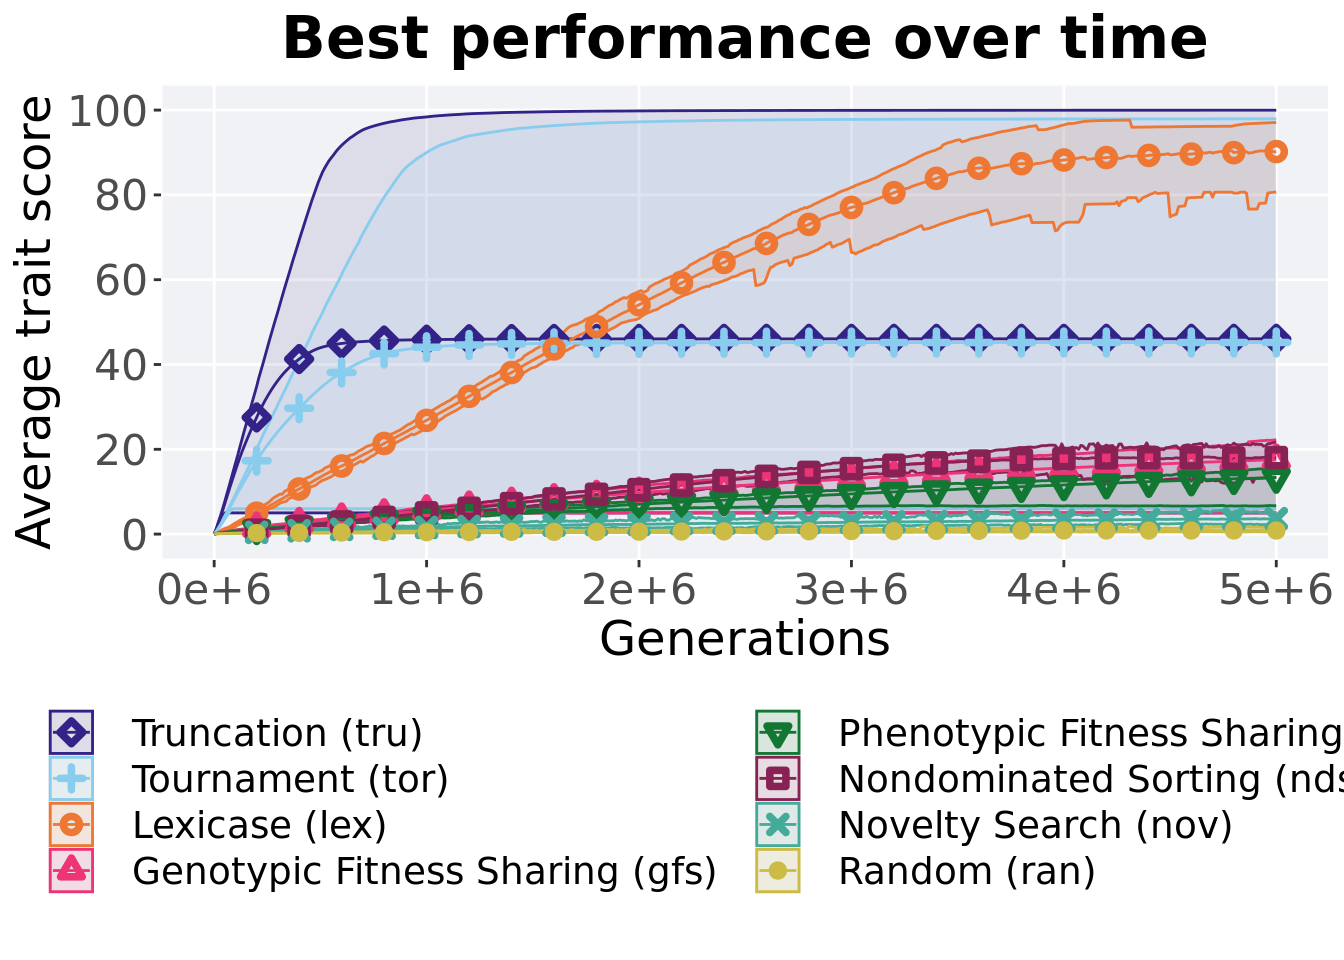
\includegraphics{demo_files/figure-latex/mpe-per-ot-1.pdf}

\hypertarget{best-performance-throughout-4}{%
\subsection{Best performance throughout}\label{best-performance-throughout-4}}

Best performance throughout 50,000 generations.

\begin{Shaded}
\begin{Highlighting}[]
\CommentTok{### best performance throughout}
\KeywordTok{filter}\NormalTok{(cc_best, col }\OperatorTok{==}\StringTok{ 'pop_fit_max'} \OperatorTok{&}\StringTok{ }\NormalTok{diagnostic }\OperatorTok{==}\StringTok{ 'multipath_exploration'}\NormalTok{) }\OperatorTok
\StringTok{  }\KeywordTok{ggplot}\NormalTok{(., }\KeywordTok{aes}\NormalTok{(}\DataTypeTok{x =}\NormalTok{ acron, }\DataTypeTok{y =}\NormalTok{ val }\OperatorTok{/}\StringTok{ }\NormalTok{DIMENSIONALITY, }\DataTypeTok{color =}\NormalTok{ acron, }\DataTypeTok{fill =}\NormalTok{ acron, }\DataTypeTok{shape =}\NormalTok{ acron)) }\OperatorTok{+}
\StringTok{  }\KeywordTok{geom_flat_violin}\NormalTok{(}\DataTypeTok{position =} \KeywordTok{position_nudge}\NormalTok{(}\DataTypeTok{x =} \FloatTok{.2}\NormalTok{, }\DataTypeTok{y =} \DecValTok{0}\NormalTok{), }\DataTypeTok{scale =} \StringTok{'width'}\NormalTok{, }\DataTypeTok{alpha =} \FloatTok{0.2}\NormalTok{) }\OperatorTok{+}
\StringTok{  }\KeywordTok{geom_point}\NormalTok{(}\DataTypeTok{position =} \KeywordTok{position_jitter}\NormalTok{(}\DataTypeTok{width =} \FloatTok{.1}\NormalTok{), }\DataTypeTok{size =} \FloatTok{1.5}\NormalTok{, }\DataTypeTok{alpha =} \FloatTok{1.0}\NormalTok{) }\OperatorTok{+}
\StringTok{  }\KeywordTok{geom_boxplot}\NormalTok{(}\DataTypeTok{color =} \StringTok{'black'}\NormalTok{, }\DataTypeTok{width =} \FloatTok{.2}\NormalTok{, }\DataTypeTok{outlier.shape =} \OtherTok{NA}\NormalTok{, }\DataTypeTok{alpha =} \FloatTok{0.0}\NormalTok{) }\OperatorTok{+}
\StringTok{  }\KeywordTok{guides}\NormalTok{(}\DataTypeTok{fill =} \StringTok{"none"}\NormalTok{,}\DataTypeTok{color =} \StringTok{'none'}\NormalTok{, }\DataTypeTok{shape =} \StringTok{'none'}\NormalTok{) }\OperatorTok{+}
\StringTok{  }\KeywordTok{scale_y_continuous}\NormalTok{(}
    \DataTypeTok{name=}\StringTok{"Average trait score"}\NormalTok{,}
    \DataTypeTok{limits=}\KeywordTok{c}\NormalTok{(}\OperatorTok{-}\DecValTok{1}\NormalTok{, }\DecValTok{101}\NormalTok{),}
    \DataTypeTok{breaks=}\KeywordTok{seq}\NormalTok{(}\DecValTok{0}\NormalTok{,}\DecValTok{100}\NormalTok{, }\DecValTok{20}\NormalTok{),}
    \DataTypeTok{labels=}\KeywordTok{c}\NormalTok{(}\StringTok{"0"}\NormalTok{, }\StringTok{"20"}\NormalTok{, }\StringTok{"40"}\NormalTok{, }\StringTok{"60"}\NormalTok{, }\StringTok{"80"}\NormalTok{, }\StringTok{"100"}\NormalTok{)}
\NormalTok{  ) }\OperatorTok{+}
\StringTok{  }\KeywordTok{scale_x_discrete}\NormalTok{(}
    \DataTypeTok{name=}\StringTok{"Scheme"}
\NormalTok{  )}\OperatorTok{+}
\StringTok{  }\KeywordTok{scale_shape_manual}\NormalTok{(}\DataTypeTok{values=}\NormalTok{SHAPE)}\OperatorTok{+}
\StringTok{  }\KeywordTok{scale_colour_manual}\NormalTok{(}\DataTypeTok{values =}\NormalTok{ cb_palette, ) }\OperatorTok{+}
\StringTok{  }\KeywordTok{scale_fill_manual}\NormalTok{(}\DataTypeTok{values =}\NormalTok{ cb_palette) }\OperatorTok{+}
\StringTok{  }\KeywordTok{ggtitle}\NormalTok{(}\StringTok{'Best performance throughout'}\NormalTok{)}\OperatorTok{+}
\StringTok{  }\NormalTok{p_theme }\OperatorTok{+}\StringTok{ }\KeywordTok{theme}\NormalTok{(}\DataTypeTok{legend.title=}\KeywordTok{element_blank}\NormalTok{()) }\OperatorTok{+}
\StringTok{  }\KeywordTok{guides}\NormalTok{(}
    \DataTypeTok{shape=}\KeywordTok{guide_legend}\NormalTok{(}\DataTypeTok{nrow=}\DecValTok{2}\NormalTok{, }\DataTypeTok{title.position =} \StringTok{"bottom"}\NormalTok{),}
    \DataTypeTok{color=}\KeywordTok{guide_legend}\NormalTok{(}\DataTypeTok{nrow=}\DecValTok{2}\NormalTok{, }\DataTypeTok{title.position =} \StringTok{"bottom"}\NormalTok{),}
    \DataTypeTok{fill=}\KeywordTok{guide_legend}\NormalTok{(}\DataTypeTok{nrow=}\DecValTok{2}\NormalTok{, }\DataTypeTok{title.position =} \StringTok{"bottom"}\NormalTok{)}
\NormalTok{  )}
\end{Highlighting}
\end{Shaded}

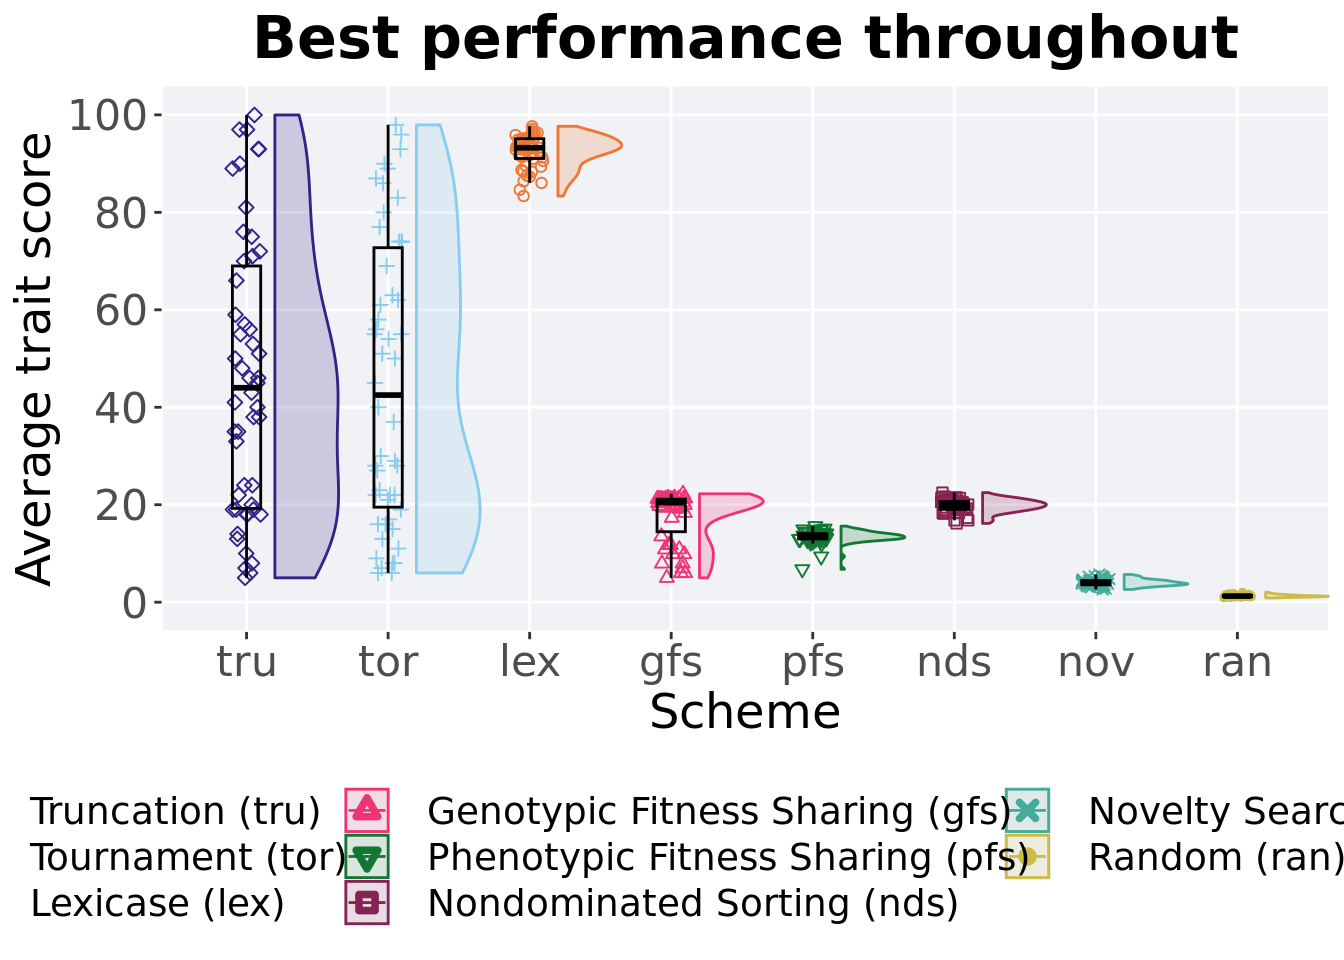
\includegraphics{demo_files/figure-latex/mpe-per-bst-1.pdf}

\hypertarget{stats-16}{%
\subsubsection{Stats}\label{stats-16}}

Summary statistics for the best performance.

\begin{Shaded}
\begin{Highlighting}[]
\CommentTok{### best performance throughout}
\NormalTok{performance =}\StringTok{ }\KeywordTok{filter}\NormalTok{(cc_best, col }\OperatorTok{==}\StringTok{ 'pop_fit_max'} \OperatorTok{&}\StringTok{ }\NormalTok{diagnostic }\OperatorTok{==}\StringTok{ 'multipath_exploration'}\NormalTok{)}
\NormalTok{performance}\OperatorTok{$}\NormalTok{acron =}\StringTok{ }\KeywordTok{factor}\NormalTok{(performance}\OperatorTok{$}\NormalTok{acron, }\DataTypeTok{levels =} \KeywordTok{c}\NormalTok{(}\StringTok{'lex'}\NormalTok{,}\StringTok{'tor'}\NormalTok{,}\StringTok{'tru'}\NormalTok{,}\StringTok{'nds'}\NormalTok{,}\StringTok{'gfs'}\NormalTok{,}\StringTok{'pfs'}\NormalTok{,}\StringTok{'nov'}\NormalTok{,}\StringTok{'ran'}\NormalTok{))}
\NormalTok{performance }\OperatorTok
\StringTok{  }\KeywordTok{group_by}\NormalTok{(acron) }\OperatorTok
\StringTok{  }\NormalTok{dplyr}\OperatorTok{::}\KeywordTok{summarise}\NormalTok{(}
    \DataTypeTok{count =} \KeywordTok{n}\NormalTok{(),}
    \DataTypeTok{na_cnt =} \KeywordTok{sum}\NormalTok{(}\KeywordTok{is.na}\NormalTok{(val)),}
    \DataTypeTok{min =} \KeywordTok{min}\NormalTok{(val }\OperatorTok{/}\StringTok{ }\NormalTok{DIMENSIONALITY, }\DataTypeTok{na.rm =} \OtherTok{TRUE}\NormalTok{),}
    \DataTypeTok{median =} \KeywordTok{median}\NormalTok{(val }\OperatorTok{/}\StringTok{ }\NormalTok{DIMENSIONALITY, }\DataTypeTok{na.rm =} \OtherTok{TRUE}\NormalTok{),}
    \DataTypeTok{mean =} \KeywordTok{mean}\NormalTok{(val }\OperatorTok{/}\StringTok{ }\NormalTok{DIMENSIONALITY, }\DataTypeTok{na.rm =} \OtherTok{TRUE}\NormalTok{),}
    \DataTypeTok{max =} \KeywordTok{max}\NormalTok{(val }\OperatorTok{/}\StringTok{ }\NormalTok{DIMENSIONALITY, }\DataTypeTok{na.rm =} \OtherTok{TRUE}\NormalTok{),}
    \DataTypeTok{IQR =} \KeywordTok{IQR}\NormalTok{(val }\OperatorTok{/}\StringTok{ }\NormalTok{DIMENSIONALITY, }\DataTypeTok{na.rm =} \OtherTok{TRUE}\NormalTok{)}
\NormalTok{  )}
\end{Highlighting}
\end{Shaded}

\begin{verbatim}
## # A tibble: 8 x 8
##   acron count na_cnt    min median  mean    max    IQR
##   <fct> <int>  <int>  <dbl>  <dbl> <dbl>  <dbl>  <dbl>
## 1 lex      50      0 83.4    93.2  92.5   97.7   4.05 
## 2 tor      50      0  6.00   42.5  45.2   97.9  53.2  
## 3 tru      50      0  5      44.0  46.1  100.   49.7  
## 4 nds      50      0 16.2    19.9  19.8   22.5   1.59 
## 5 gfs      50      0  4.99   20.4  17.6   22.2   6.69 
## 6 pfs      50      0  6.76   13.5  13.4   15.6   1.10 
## 7 nov      50      0  2.62    3.89  4.01   5.68  0.860
## 8 ran      50      0  0.870   1.25  1.28   2.04  0.288
\end{verbatim}

Kruskal--Wallis test provides evidence of difference among best performances.

\begin{Shaded}
\begin{Highlighting}[]
\KeywordTok{kruskal.test}\NormalTok{(val }\OperatorTok{~}\StringTok{ }\NormalTok{acron, }\DataTypeTok{data =}\NormalTok{ performance)}
\end{Highlighting}
\end{Shaded}

\begin{verbatim}
## 
##  Kruskal-Wallis rank sum test
## 
## data:  val by acron
## Kruskal-Wallis chi-squared = 329.88, df = 7, p-value < 2.2e-16
\end{verbatim}

Results for post-hoc Wilcoxon rank-sum test with a Bonferroni correction on best performance.

\begin{Shaded}
\begin{Highlighting}[]
\KeywordTok{pairwise.wilcox.test}\NormalTok{(}\DataTypeTok{x =}\NormalTok{ performance}\OperatorTok{$}\NormalTok{val, }\DataTypeTok{g =}\NormalTok{ performance}\OperatorTok{$}\NormalTok{acron, }\DataTypeTok{p.adjust.method =} \StringTok{"bonferroni"}\NormalTok{,}
                     \DataTypeTok{paired =} \OtherTok{FALSE}\NormalTok{, }\DataTypeTok{conf.int =} \OtherTok{FALSE}\NormalTok{, }\DataTypeTok{alternative =} \StringTok{'l'}\NormalTok{)}
\end{Highlighting}
\end{Shaded}

\begin{verbatim}
## 
##  Pairwise comparisons using Wilcoxon rank sum test with continuity correction 
## 
## data:  performance$val and performance$acron 
## 
##     lex     tor     tru     nds     gfs     pfs     nov    
## tor 3.0e-13 -       -       -       -       -       -      
## tru 1.1e-11 1.00000 -       -       -       -       -      
## nds < 2e-16 0.00047 0.00027 -       -       -       -      
## gfs < 2e-16 2.3e-05 1.6e-05 1.00000 -       -       -      
## pfs < 2e-16 3.1e-08 6.9e-10 < 2e-16 0.00015 -       -      
## nov < 2e-16 < 2e-16 < 2e-16 < 2e-16 < 2e-16 < 2e-16 -      
## ran < 2e-16 < 2e-16 < 2e-16 < 2e-16 < 2e-16 < 2e-16 < 2e-16
## 
## P value adjustment method: bonferroni
\end{verbatim}

\hypertarget{end-of-50000-generations-3}{%
\subsection{End of 50,000 generations}\label{end-of-50000-generations-3}}

Best performance in the population at the end of 50,000 generations.

\begin{Shaded}
\begin{Highlighting}[]
\CommentTok{# end of run}
\KeywordTok{filter}\NormalTok{(cc_over_time, diagnostic }\OperatorTok{==}\StringTok{ 'multipath_exploration'} \OperatorTok{&}\StringTok{ }\NormalTok{gen }\OperatorTok{==}\StringTok{ }\DecValTok{50000}\NormalTok{) }\OperatorTok
\StringTok{  }\KeywordTok{ggplot}\NormalTok{(., }\KeywordTok{aes}\NormalTok{(}\DataTypeTok{x =}\NormalTok{ acron, }\DataTypeTok{y =}\NormalTok{ pop_fit_max }\OperatorTok{/}\StringTok{ }\NormalTok{DIMENSIONALITY, }\DataTypeTok{color =}\NormalTok{ acron, }\DataTypeTok{fill =}\NormalTok{ acron, }\DataTypeTok{shape =}\NormalTok{ acron)) }\OperatorTok{+}
\StringTok{  }\KeywordTok{geom_flat_violin}\NormalTok{(}\DataTypeTok{position =} \KeywordTok{position_nudge}\NormalTok{(}\DataTypeTok{x =} \FloatTok{.2}\NormalTok{, }\DataTypeTok{y =} \DecValTok{0}\NormalTok{), }\DataTypeTok{scale =} \StringTok{'width'}\NormalTok{, }\DataTypeTok{alpha =} \FloatTok{0.2}\NormalTok{) }\OperatorTok{+}
\StringTok{  }\KeywordTok{geom_point}\NormalTok{(}\DataTypeTok{position =} \KeywordTok{position_jitter}\NormalTok{(}\DataTypeTok{width =} \FloatTok{.1}\NormalTok{), }\DataTypeTok{size =} \FloatTok{1.5}\NormalTok{, }\DataTypeTok{alpha =} \FloatTok{1.0}\NormalTok{) }\OperatorTok{+}
\StringTok{  }\KeywordTok{geom_boxplot}\NormalTok{(}\DataTypeTok{color =} \StringTok{'black'}\NormalTok{, }\DataTypeTok{width =} \FloatTok{.2}\NormalTok{, }\DataTypeTok{outlier.shape =} \OtherTok{NA}\NormalTok{, }\DataTypeTok{alpha =} \FloatTok{0.0}\NormalTok{) }\OperatorTok{+}
\StringTok{  }\KeywordTok{guides}\NormalTok{(}\DataTypeTok{fill =} \StringTok{"none"}\NormalTok{,}\DataTypeTok{color =} \StringTok{'none'}\NormalTok{, }\DataTypeTok{shape =} \StringTok{'none'}\NormalTok{) }\OperatorTok{+}
\StringTok{  }\KeywordTok{scale_y_continuous}\NormalTok{(}
    \DataTypeTok{name=}\StringTok{"Coverage"}\NormalTok{,}
    \DataTypeTok{limits=}\KeywordTok{c}\NormalTok{(}\DecValTok{0}\NormalTok{, }\DecValTok{100}\NormalTok{),}
    \DataTypeTok{breaks=}\KeywordTok{seq}\NormalTok{(}\DecValTok{0}\NormalTok{,}\DecValTok{100}\NormalTok{, }\DecValTok{20}\NormalTok{),}
    \DataTypeTok{labels=}\KeywordTok{c}\NormalTok{(}\StringTok{"0"}\NormalTok{, }\StringTok{"20"}\NormalTok{, }\StringTok{"40"}\NormalTok{, }\StringTok{"60"}\NormalTok{, }\StringTok{"80"}\NormalTok{, }\StringTok{"100"}\NormalTok{)}
\NormalTok{  ) }\OperatorTok{+}
\StringTok{  }\KeywordTok{scale_x_discrete}\NormalTok{(}
    \DataTypeTok{name=}\StringTok{"Scheme"}
\NormalTok{  )}\OperatorTok{+}
\StringTok{  }\KeywordTok{scale_shape_manual}\NormalTok{(}\DataTypeTok{values=}\NormalTok{SHAPE)}\OperatorTok{+}
\StringTok{  }\KeywordTok{scale_colour_manual}\NormalTok{(}\DataTypeTok{values =}\NormalTok{ cb_palette, ) }\OperatorTok{+}
\StringTok{  }\KeywordTok{scale_fill_manual}\NormalTok{(}\DataTypeTok{values =}\NormalTok{ cb_palette) }\OperatorTok{+}
\StringTok{  }\KeywordTok{ggtitle}\NormalTok{(}\StringTok{'Final performance'}\NormalTok{)}\OperatorTok{+}
\StringTok{  }\NormalTok{p_theme }\OperatorTok{+}\StringTok{ }\KeywordTok{theme}\NormalTok{(}\DataTypeTok{legend.title=}\KeywordTok{element_blank}\NormalTok{()) }\OperatorTok{+}
\StringTok{  }\KeywordTok{guides}\NormalTok{(}
    \DataTypeTok{shape=}\KeywordTok{guide_legend}\NormalTok{(}\DataTypeTok{nrow=}\DecValTok{2}\NormalTok{, }\DataTypeTok{title.position =} \StringTok{"bottom"}\NormalTok{),}
    \DataTypeTok{color=}\KeywordTok{guide_legend}\NormalTok{(}\DataTypeTok{nrow=}\DecValTok{2}\NormalTok{, }\DataTypeTok{title.position =} \StringTok{"bottom"}\NormalTok{),}
    \DataTypeTok{fill=}\KeywordTok{guide_legend}\NormalTok{(}\DataTypeTok{nrow=}\DecValTok{2}\NormalTok{, }\DataTypeTok{title.position =} \StringTok{"bottom"}\NormalTok{)}
\NormalTok{  )}
\end{Highlighting}
\end{Shaded}

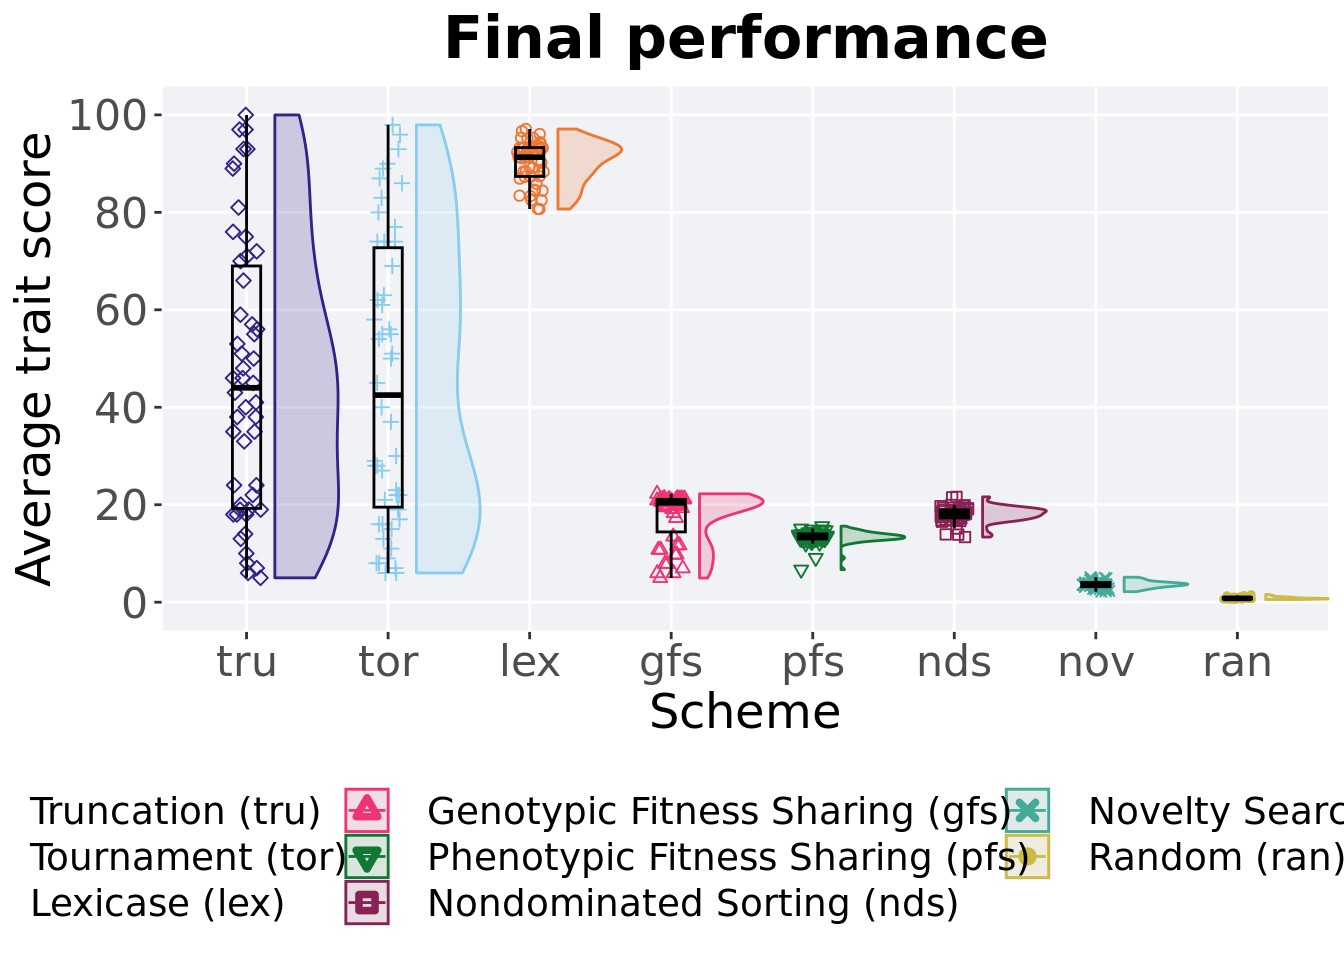
\includegraphics{demo_files/figure-latex/mpe-per-end-1.pdf}

\hypertarget{stats-17}{%
\subsubsection{Stats}\label{stats-17}}

Summary statistics for best performance in the final population.

\begin{Shaded}
\begin{Highlighting}[]
\CommentTok{# end of run}
\NormalTok{performance =}\StringTok{ }\KeywordTok{filter}\NormalTok{(cc_over_time, diagnostic }\OperatorTok{==}\StringTok{ 'multipath_exploration'} \OperatorTok{&}\StringTok{ }\NormalTok{gen }\OperatorTok{==}\StringTok{ }\DecValTok{50000}\NormalTok{)}
\NormalTok{performance}\OperatorTok{$}\NormalTok{acron =}\StringTok{ }\KeywordTok{factor}\NormalTok{(performance}\OperatorTok{$}\NormalTok{acron, }\DataTypeTok{levels =} \KeywordTok{c}\NormalTok{(}\StringTok{'lex'}\NormalTok{,}\StringTok{'tor'}\NormalTok{,}\StringTok{'tru'}\NormalTok{,}\StringTok{'nds'}\NormalTok{,}\StringTok{'gfs'}\NormalTok{,}\StringTok{'pfs'}\NormalTok{,}\StringTok{'nov'}\NormalTok{,}\StringTok{'ran'}\NormalTok{))}
\NormalTok{performance }\OperatorTok
\StringTok{  }\KeywordTok{group_by}\NormalTok{(acron) }\OperatorTok
\StringTok{  }\NormalTok{dplyr}\OperatorTok{::}\KeywordTok{summarise}\NormalTok{(}
    \DataTypeTok{count =} \KeywordTok{n}\NormalTok{(),}
    \DataTypeTok{na_cnt =} \KeywordTok{sum}\NormalTok{(}\KeywordTok{is.na}\NormalTok{(pop_fit_max }\OperatorTok{/}\StringTok{ }\NormalTok{DIMENSIONALITY)),}
    \DataTypeTok{min =} \KeywordTok{min}\NormalTok{(pop_fit_max }\OperatorTok{/}\StringTok{ }\NormalTok{DIMENSIONALITY, }\DataTypeTok{na.rm =} \OtherTok{TRUE}\NormalTok{),}
    \DataTypeTok{median =} \KeywordTok{median}\NormalTok{(pop_fit_max }\OperatorTok{/}\StringTok{ }\NormalTok{DIMENSIONALITY, }\DataTypeTok{na.rm =} \OtherTok{TRUE}\NormalTok{),}
    \DataTypeTok{mean =} \KeywordTok{mean}\NormalTok{(pop_fit_max }\OperatorTok{/}\StringTok{ }\NormalTok{DIMENSIONALITY, }\DataTypeTok{na.rm =} \OtherTok{TRUE}\NormalTok{),}
    \DataTypeTok{max =} \KeywordTok{max}\NormalTok{(pop_fit_max }\OperatorTok{/}\StringTok{ }\NormalTok{DIMENSIONALITY, }\DataTypeTok{na.rm =} \OtherTok{TRUE}\NormalTok{),}
    \DataTypeTok{IQR =} \KeywordTok{IQR}\NormalTok{(pop_fit_max }\OperatorTok{/}\StringTok{ }\NormalTok{DIMENSIONALITY, }\DataTypeTok{na.rm =} \OtherTok{TRUE}\NormalTok{)}
\NormalTok{  )}
\end{Highlighting}
\end{Shaded}

\begin{verbatim}
## # A tibble: 8 x 8
##   acron count na_cnt    min median   mean    max    IQR
##   <fct> <int>  <int>  <dbl>  <dbl>  <dbl>  <dbl>  <dbl>
## 1 lex      50      0 80.7   91.3   90.2    97.1   5.91 
## 2 tor      50      0  6.00  42.5   45.2    97.9  53.2  
## 3 tru      50      0  5     44.0   46.1   100.   49.7  
## 4 nds      50      0 13.4   18.1   18.0    21.6   1.65 
## 5 gfs      50      0  4.96  20.4   17.6    22.2   6.68 
## 6 pfs      50      0  6.67  13.5   13.3    15.6   1.04 
## 7 nov      50      0  2.16   3.66   3.64    5.12  0.859
## 8 ran      50      0  0.553  0.785  0.840   1.56  0.299
\end{verbatim}

Kruskal--Wallis test provides evidence of difference among best performance in the final population.

\begin{Shaded}
\begin{Highlighting}[]
\KeywordTok{kruskal.test}\NormalTok{(pop_fit_max }\OperatorTok{~}\StringTok{ }\NormalTok{acron, }\DataTypeTok{data =}\NormalTok{ performance)}
\end{Highlighting}
\end{Shaded}

\begin{verbatim}
## 
##  Kruskal-Wallis rank sum test
## 
## data:  pop_fit_max by acron
## Kruskal-Wallis chi-squared = 330.05, df = 7, p-value < 2.2e-16
\end{verbatim}

Results for post-hoc Wilcoxon rank-sum test with a Bonferroni correction on best performance in the final population.

\begin{Shaded}
\begin{Highlighting}[]
\KeywordTok{pairwise.wilcox.test}\NormalTok{(}\DataTypeTok{x =}\NormalTok{ performance}\OperatorTok{$}\NormalTok{pop_fit_max, }\DataTypeTok{g =}\NormalTok{ performance}\OperatorTok{$}\NormalTok{acron, }\DataTypeTok{p.adjust.method =} \StringTok{"bonferroni"}\NormalTok{,}
                     \DataTypeTok{paired =} \OtherTok{FALSE}\NormalTok{, }\DataTypeTok{conf.int =} \OtherTok{FALSE}\NormalTok{, }\DataTypeTok{alternative =} \StringTok{'l'}\NormalTok{)}
\end{Highlighting}
\end{Shaded}

\begin{verbatim}
## 
##  Pairwise comparisons using Wilcoxon rank sum test with continuity correction 
## 
## data:  performance$pop_fit_max and performance$acron 
## 
##     lex     tor     tru     nds     gfs     pfs     nov    
## tor 3.9e-12 -       -       -       -       -       -      
## tru 7.1e-11 1.00000 -       -       -       -       -      
## nds < 2e-16 8.2e-05 9.3e-07 -       -       -       -      
## gfs < 2e-16 2.2e-05 1.6e-05 1.00000 -       -       -      
## pfs < 2e-16 3.0e-08 6.6e-10 3.0e-15 0.00015 -       -      
## nov < 2e-16 < 2e-16 < 2e-16 < 2e-16 < 2e-16 < 2e-16 -      
## ran < 2e-16 < 2e-16 < 2e-16 < 2e-16 < 2e-16 < 2e-16 < 2e-16
## 
## P value adjustment method: bonferroni
\end{verbatim}

\hypertarget{activation-gene-coverage-2}{%
\section{Activation gene coverage}\label{activation-gene-coverage-2}}

Activation gene coverage analysis.

\hypertarget{over-time-coverage-1}{%
\subsection{Over time coverage}\label{over-time-coverage-1}}

Activation gene coverage over time.

\begin{Shaded}
\begin{Highlighting}[]
\CommentTok{# data for lines and shading on plots}
\NormalTok{lines =}\StringTok{ }\KeywordTok{filter}\NormalTok{(cc_over_time, diagnostic }\OperatorTok{==}\StringTok{ 'multipath_exploration'}\NormalTok{) }\OperatorTok
\StringTok{  }\KeywordTok{group_by}\NormalTok{(}\StringTok{`}\DataTypeTok{Selection}\CharTok{\textbackslash{}n}\DataTypeTok{Scheme}\StringTok{`}\NormalTok{, gen) }\OperatorTok
\StringTok{  }\NormalTok{dplyr}\OperatorTok{::}\KeywordTok{summarise}\NormalTok{(}
    \DataTypeTok{min =} \KeywordTok{min}\NormalTok{(uni_str_pos),}
    \DataTypeTok{mean =} \KeywordTok{mean}\NormalTok{(uni_str_pos),}
    \DataTypeTok{max =} \KeywordTok{max}\NormalTok{(uni_str_pos)}
\NormalTok{  )}
\end{Highlighting}
\end{Shaded}

\begin{verbatim}
## `summarise()` has grouped output by 'Selection Scheme'. You can override using
## the `.groups` argument.
\end{verbatim}

\begin{Shaded}
\begin{Highlighting}[]
\KeywordTok{ggplot}\NormalTok{(lines, }\KeywordTok{aes}\NormalTok{(}\DataTypeTok{x=}\NormalTok{gen, }\DataTypeTok{y=}\NormalTok{mean, }\DataTypeTok{group =} \StringTok{`}\DataTypeTok{Selection}\CharTok{\textbackslash{}n}\DataTypeTok{Scheme}\StringTok{`}\NormalTok{, }\DataTypeTok{fill =}\StringTok{`}\DataTypeTok{Selection}\CharTok{\textbackslash{}n}\DataTypeTok{Scheme}\StringTok{`}\NormalTok{, }\DataTypeTok{color =} \StringTok{`}\DataTypeTok{Selection}\CharTok{\textbackslash{}n}\DataTypeTok{Scheme}\StringTok{`}\NormalTok{, }\DataTypeTok{shape =} \StringTok{`}\DataTypeTok{Selection}\CharTok{\textbackslash{}n}\DataTypeTok{Scheme}\StringTok{`}\NormalTok{)) }\OperatorTok{+}
\StringTok{  }\KeywordTok{geom_ribbon}\NormalTok{(}\KeywordTok{aes}\NormalTok{(}\DataTypeTok{ymin =}\NormalTok{ min, }\DataTypeTok{ymax =}\NormalTok{ max), }\DataTypeTok{alpha =} \FloatTok{0.1}\NormalTok{) }\OperatorTok{+}
\StringTok{  }\KeywordTok{geom_line}\NormalTok{(}\DataTypeTok{size =} \FloatTok{0.5}\NormalTok{) }\OperatorTok{+}
\StringTok{  }\KeywordTok{geom_point}\NormalTok{(}\DataTypeTok{data =} \KeywordTok{filter}\NormalTok{(lines, gen }\OperatorTok\StringTok{ }\DecValTok{2000} \OperatorTok{==}\StringTok{ }\DecValTok{0} \OperatorTok{&}\StringTok{ }\NormalTok{gen }\OperatorTok{!=}\StringTok{ }\DecValTok{0}\NormalTok{), }\DataTypeTok{size =} \FloatTok{1.5}\NormalTok{, }\DataTypeTok{stroke =} \FloatTok{2.0}\NormalTok{, }\DataTypeTok{alpha =} \FloatTok{1.0}\NormalTok{) }\OperatorTok{+}
\StringTok{  }\KeywordTok{scale_y_continuous}\NormalTok{(}
    \DataTypeTok{name=}\StringTok{"Coverage"}\NormalTok{,}
    \DataTypeTok{limits=}\KeywordTok{c}\NormalTok{(}\DecValTok{0}\NormalTok{, }\DecValTok{100}\NormalTok{),}
    \DataTypeTok{breaks=}\KeywordTok{seq}\NormalTok{(}\DecValTok{0}\NormalTok{,}\DecValTok{100}\NormalTok{, }\DecValTok{20}\NormalTok{),}
    \DataTypeTok{labels=}\KeywordTok{c}\NormalTok{(}\StringTok{"0"}\NormalTok{, }\StringTok{"20"}\NormalTok{, }\StringTok{"40"}\NormalTok{, }\StringTok{"60"}\NormalTok{, }\StringTok{"80"}\NormalTok{, }\StringTok{"100"}\NormalTok{)}
\NormalTok{  ) }\OperatorTok{+}
\StringTok{  }\KeywordTok{scale_x_continuous}\NormalTok{(}
    \DataTypeTok{name=}\StringTok{"Generations"}\NormalTok{,}
    \DataTypeTok{limits=}\KeywordTok{c}\NormalTok{(}\DecValTok{0}\NormalTok{, }\DecValTok{50000}\NormalTok{),}
    \DataTypeTok{breaks=}\KeywordTok{c}\NormalTok{(}\DecValTok{0}\NormalTok{, }\DecValTok{10000}\NormalTok{, }\DecValTok{20000}\NormalTok{, }\DecValTok{30000}\NormalTok{, }\DecValTok{40000}\NormalTok{, }\DecValTok{50000}\NormalTok{),}
    \DataTypeTok{labels=}\KeywordTok{c}\NormalTok{(}\StringTok{"0e+4"}\NormalTok{, }\StringTok{"1e+4"}\NormalTok{, }\StringTok{"2e+4"}\NormalTok{, }\StringTok{"3e+4"}\NormalTok{, }\StringTok{"4e+4"}\NormalTok{, }\StringTok{"5e+4"}\NormalTok{)}
\NormalTok{  ) }\OperatorTok{+}
\StringTok{  }\KeywordTok{scale_shape_manual}\NormalTok{(}\DataTypeTok{values=}\NormalTok{SHAPE)}\OperatorTok{+}
\StringTok{  }\KeywordTok{scale_colour_manual}\NormalTok{(}\DataTypeTok{values =}\NormalTok{ cb_palette) }\OperatorTok{+}
\StringTok{  }\KeywordTok{scale_fill_manual}\NormalTok{(}\DataTypeTok{values =}\NormalTok{ cb_palette) }\OperatorTok{+}
\StringTok{  }\KeywordTok{ggtitle}\NormalTok{(}\StringTok{'Activation gene coverage over time'}\NormalTok{)}\OperatorTok{+}
\StringTok{  }\NormalTok{p_theme }\OperatorTok{+}\StringTok{ }\KeywordTok{theme}\NormalTok{(}\DataTypeTok{legend.title=}\KeywordTok{element_blank}\NormalTok{(),}\DataTypeTok{legend.text=}\KeywordTok{element_text}\NormalTok{(}\DataTypeTok{size=}\DecValTok{11}\NormalTok{)) }\OperatorTok{+}
\StringTok{  }\KeywordTok{guides}\NormalTok{(}
    \DataTypeTok{shape=}\KeywordTok{guide_legend}\NormalTok{(}\DataTypeTok{ncol=}\DecValTok{2}\NormalTok{, }\DataTypeTok{title.position =} \StringTok{"bottom"}\NormalTok{),}
    \DataTypeTok{color=}\KeywordTok{guide_legend}\NormalTok{(}\DataTypeTok{ncol=}\DecValTok{2}\NormalTok{, }\DataTypeTok{title.position =} \StringTok{"bottom"}\NormalTok{),}
    \DataTypeTok{fill=}\KeywordTok{guide_legend}\NormalTok{(}\DataTypeTok{ncol=}\DecValTok{2}\NormalTok{, }\DataTypeTok{title.position =} \StringTok{"bottom"}\NormalTok{)}
\NormalTok{  )}
\end{Highlighting}
\end{Shaded}

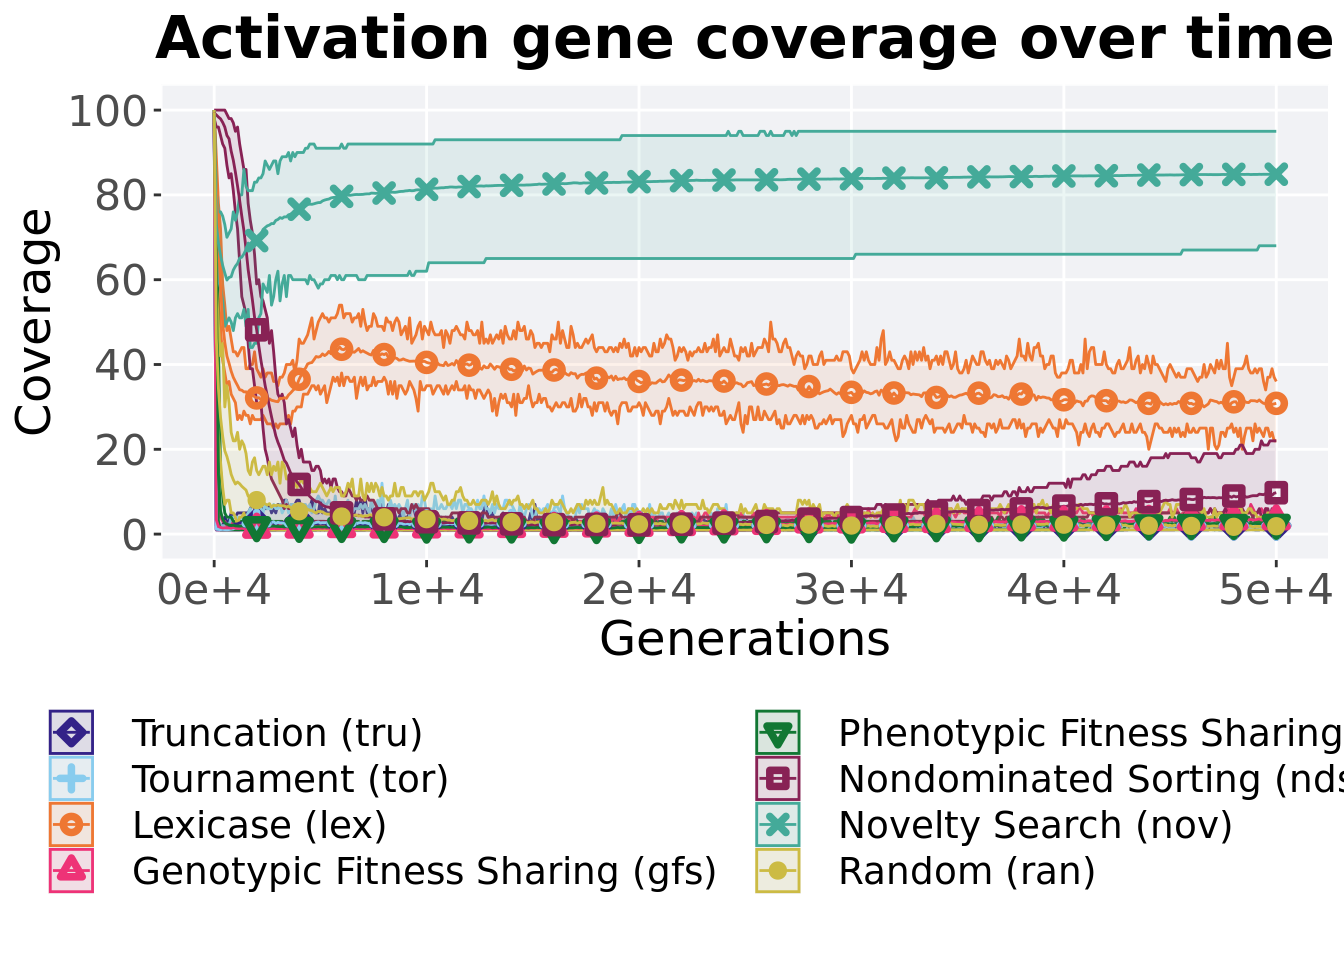
\includegraphics{demo_files/figure-latex/mpe-act-ot-1.pdf}

\hypertarget{end-of-50000-generations-4}{%
\subsection{End of 50,000 generations}\label{end-of-50000-generations-4}}

Activation gene coverage in the population at the end of 50,000 generations.

\begin{Shaded}
\begin{Highlighting}[]
\CommentTok{# end of run}
\KeywordTok{filter}\NormalTok{(cc_over_time, diagnostic }\OperatorTok{==}\StringTok{ 'multipath_exploration'} \OperatorTok{&}\StringTok{ }\NormalTok{gen }\OperatorTok{==}\StringTok{ }\DecValTok{50000}\NormalTok{) }\OperatorTok
\StringTok{  }\KeywordTok{ggplot}\NormalTok{(., }\KeywordTok{aes}\NormalTok{(}\DataTypeTok{x =}\NormalTok{ acron, }\DataTypeTok{y =}\NormalTok{ uni_str_pos, }\DataTypeTok{color =}\NormalTok{ acron, }\DataTypeTok{fill =}\NormalTok{ acron, }\DataTypeTok{shape =}\NormalTok{ acron)) }\OperatorTok{+}
\StringTok{  }\KeywordTok{geom_flat_violin}\NormalTok{(}\DataTypeTok{position =} \KeywordTok{position_nudge}\NormalTok{(}\DataTypeTok{x =} \FloatTok{.2}\NormalTok{, }\DataTypeTok{y =} \DecValTok{0}\NormalTok{), }\DataTypeTok{scale =} \StringTok{'width'}\NormalTok{, }\DataTypeTok{alpha =} \FloatTok{0.2}\NormalTok{) }\OperatorTok{+}
\StringTok{  }\KeywordTok{geom_point}\NormalTok{(}\DataTypeTok{position =} \KeywordTok{position_jitter}\NormalTok{(}\DataTypeTok{width =} \FloatTok{.1}\NormalTok{), }\DataTypeTok{size =} \FloatTok{1.5}\NormalTok{, }\DataTypeTok{alpha =} \FloatTok{1.0}\NormalTok{) }\OperatorTok{+}
\StringTok{  }\KeywordTok{geom_boxplot}\NormalTok{(}\DataTypeTok{color =} \StringTok{'black'}\NormalTok{, }\DataTypeTok{width =} \FloatTok{.2}\NormalTok{, }\DataTypeTok{outlier.shape =} \OtherTok{NA}\NormalTok{, }\DataTypeTok{alpha =} \FloatTok{0.0}\NormalTok{) }\OperatorTok{+}
\StringTok{  }\KeywordTok{guides}\NormalTok{(}\DataTypeTok{fill =} \StringTok{"none"}\NormalTok{,}\DataTypeTok{color =} \StringTok{'none'}\NormalTok{, }\DataTypeTok{shape =} \StringTok{'none'}\NormalTok{) }\OperatorTok{+}
\StringTok{  }\KeywordTok{scale_y_continuous}\NormalTok{(}
    \DataTypeTok{name=}\StringTok{"Coverage"}\NormalTok{,}
    \DataTypeTok{limits=}\KeywordTok{c}\NormalTok{(}\DecValTok{0}\NormalTok{, }\DecValTok{100}\NormalTok{),}
    \DataTypeTok{breaks=}\KeywordTok{seq}\NormalTok{(}\DecValTok{0}\NormalTok{,}\DecValTok{100}\NormalTok{, }\DecValTok{20}\NormalTok{),}
    \DataTypeTok{labels=}\KeywordTok{c}\NormalTok{(}\StringTok{"0"}\NormalTok{, }\StringTok{"20"}\NormalTok{, }\StringTok{"40"}\NormalTok{, }\StringTok{"60"}\NormalTok{, }\StringTok{"80"}\NormalTok{, }\StringTok{"100"}\NormalTok{)}
\NormalTok{  ) }\OperatorTok{+}
\StringTok{  }\KeywordTok{scale_x_discrete}\NormalTok{(}
    \DataTypeTok{name=}\StringTok{"Scheme"}
\NormalTok{  )}\OperatorTok{+}
\StringTok{  }\KeywordTok{scale_shape_manual}\NormalTok{(}\DataTypeTok{values=}\NormalTok{SHAPE)}\OperatorTok{+}
\StringTok{  }\KeywordTok{scale_colour_manual}\NormalTok{(}\DataTypeTok{values =}\NormalTok{ cb_palette, ) }\OperatorTok{+}
\StringTok{  }\KeywordTok{scale_fill_manual}\NormalTok{(}\DataTypeTok{values =}\NormalTok{ cb_palette) }\OperatorTok{+}
\StringTok{  }\KeywordTok{ggtitle}\NormalTok{(}\StringTok{'Final activation gene coverage'}\NormalTok{)}\OperatorTok{+}
\StringTok{  }\NormalTok{p_theme }\OperatorTok{+}\StringTok{ }\KeywordTok{theme}\NormalTok{(}\DataTypeTok{legend.title=}\KeywordTok{element_blank}\NormalTok{()) }\OperatorTok{+}
\StringTok{  }\KeywordTok{guides}\NormalTok{(}
    \DataTypeTok{shape=}\KeywordTok{guide_legend}\NormalTok{(}\DataTypeTok{nrow=}\DecValTok{2}\NormalTok{, }\DataTypeTok{title.position =} \StringTok{"bottom"}\NormalTok{),}
    \DataTypeTok{color=}\KeywordTok{guide_legend}\NormalTok{(}\DataTypeTok{nrow=}\DecValTok{2}\NormalTok{, }\DataTypeTok{title.position =} \StringTok{"bottom"}\NormalTok{),}
    \DataTypeTok{fill=}\KeywordTok{guide_legend}\NormalTok{(}\DataTypeTok{nrow=}\DecValTok{2}\NormalTok{, }\DataTypeTok{title.position =} \StringTok{"bottom"}\NormalTok{)}
\NormalTok{  )}
\end{Highlighting}
\end{Shaded}

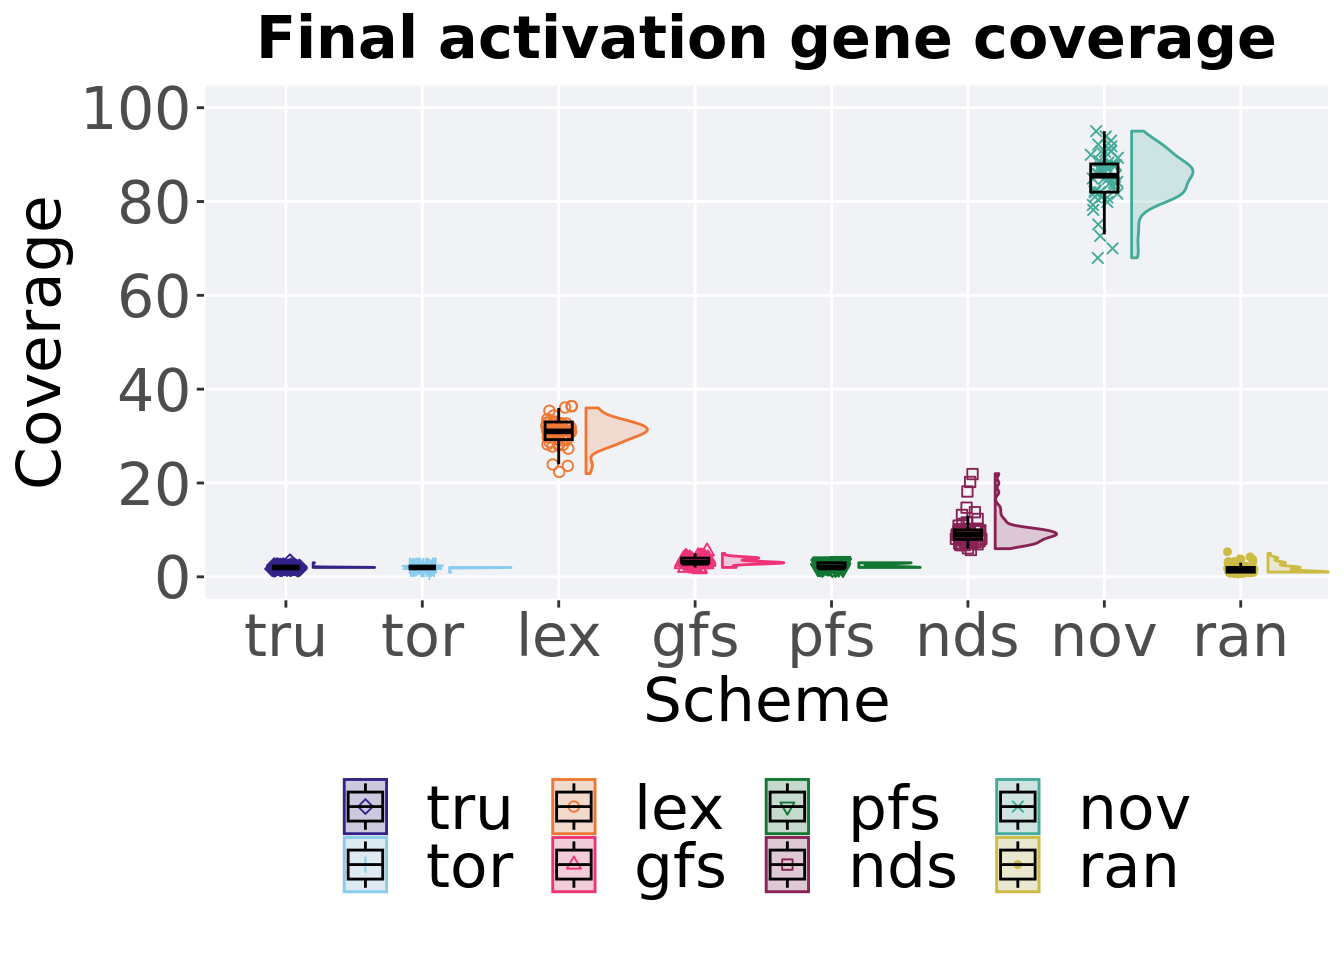
\includegraphics{demo_files/figure-latex/mpe-act-end-1.pdf}

\hypertarget{stats-18}{%
\subsubsection{Stats}\label{stats-18}}

Summary statistics for activation gene coverage in the final population.

\begin{Shaded}
\begin{Highlighting}[]
\CommentTok{# end of run}
\NormalTok{coverage =}\StringTok{ }\KeywordTok{filter}\NormalTok{(cc_over_time, diagnostic }\OperatorTok{==}\StringTok{ 'multipath_exploration'} \OperatorTok{&}\StringTok{ }\NormalTok{gen }\OperatorTok{==}\StringTok{ }\DecValTok{50000}\NormalTok{)}
\NormalTok{coverage}\OperatorTok{$}\NormalTok{acron =}\StringTok{ }\KeywordTok{factor}\NormalTok{(coverage}\OperatorTok{$}\NormalTok{acron, }\DataTypeTok{levels =} \KeywordTok{c}\NormalTok{(}\StringTok{'nov'}\NormalTok{,}\StringTok{'lex'}\NormalTok{,}\StringTok{'nds'}\NormalTok{,}\StringTok{'gfs'}\NormalTok{,}\StringTok{'pfs'}\NormalTok{,}\StringTok{'tor'}\NormalTok{,}\StringTok{'tru'}\NormalTok{,}\StringTok{'ran'}\NormalTok{))}
\NormalTok{coverage }\OperatorTok
\StringTok{  }\KeywordTok{group_by}\NormalTok{(acron) }\OperatorTok
\StringTok{  }\NormalTok{dplyr}\OperatorTok{::}\KeywordTok{summarise}\NormalTok{(}
    \DataTypeTok{count =} \KeywordTok{n}\NormalTok{(),}
    \DataTypeTok{na_cnt =} \KeywordTok{sum}\NormalTok{(}\KeywordTok{is.na}\NormalTok{(uni_str_pos)),}
    \DataTypeTok{min =} \KeywordTok{min}\NormalTok{(uni_str_pos, }\DataTypeTok{na.rm =} \OtherTok{TRUE}\NormalTok{),}
    \DataTypeTok{median =} \KeywordTok{median}\NormalTok{(uni_str_pos, }\DataTypeTok{na.rm =} \OtherTok{TRUE}\NormalTok{),}
    \DataTypeTok{mean =} \KeywordTok{mean}\NormalTok{(uni_str_pos, }\DataTypeTok{na.rm =} \OtherTok{TRUE}\NormalTok{),}
    \DataTypeTok{max =} \KeywordTok{max}\NormalTok{(uni_str_pos, }\DataTypeTok{na.rm =} \OtherTok{TRUE}\NormalTok{),}
    \DataTypeTok{IQR =} \KeywordTok{IQR}\NormalTok{(uni_str_pos, }\DataTypeTok{na.rm =} \OtherTok{TRUE}\NormalTok{)}
\NormalTok{  )}
\end{Highlighting}
\end{Shaded}

\begin{verbatim}
## # A tibble: 8 x 8
##   acron count na_cnt   min median  mean   max   IQR
##   <fct> <int>  <int> <int>  <dbl> <dbl> <int> <dbl>
## 1 nov      50      0    68   85.5 84.9     95  6   
## 2 lex      50      0    22   31   30.8     36  3.75
## 3 nds      50      0     6    9    9.76    22  2   
## 4 gfs      50      0     2    3    3.24     5  1   
## 5 pfs      50      0     2    2    2.46     3  1   
## 6 tor      50      0     1    2    1.98     2  0   
## 7 tru      50      0     2    2    2.02     3  0   
## 8 ran      50      0     1    1.5  1.86     5  1
\end{verbatim}

Kruskal--Wallis test provides evidence of difference among activation gene coverage in the final population.

\begin{Shaded}
\begin{Highlighting}[]
\KeywordTok{kruskal.test}\NormalTok{(uni_str_pos }\OperatorTok{~}\StringTok{ }\NormalTok{acron, }\DataTypeTok{data =}\NormalTok{ coverage)}
\end{Highlighting}
\end{Shaded}

\begin{verbatim}
## 
##  Kruskal-Wallis rank sum test
## 
## data:  uni_str_pos by acron
## Kruskal-Wallis chi-squared = 351.29, df = 7, p-value < 2.2e-16
\end{verbatim}

Results for post-hoc Wilcoxon rank-sum test with a Bonferroni correction on activation gene coverage in the final population.

\begin{Shaded}
\begin{Highlighting}[]
\KeywordTok{pairwise.wilcox.test}\NormalTok{(}\DataTypeTok{x =}\NormalTok{ coverage}\OperatorTok{$}\NormalTok{uni_str_pos, }\DataTypeTok{g =}\NormalTok{ coverage}\OperatorTok{$}\NormalTok{acron, }\DataTypeTok{p.adjust.method =} \StringTok{"bonferroni"}\NormalTok{,}
                     \DataTypeTok{paired =} \OtherTok{FALSE}\NormalTok{, }\DataTypeTok{conf.int =} \OtherTok{FALSE}\NormalTok{, }\DataTypeTok{alternative =} \StringTok{'l'}\NormalTok{)}
\end{Highlighting}
\end{Shaded}

\begin{verbatim}
## 
##  Pairwise comparisons using Wilcoxon rank sum test with continuity correction 
## 
## data:  coverage$uni_str_pos and coverage$acron 
## 
##     nov     lex     nds     gfs     pfs     tor     tru    
## lex < 2e-16 -       -       -       -       -       -      
## nds < 2e-16 < 2e-16 -       -       -       -       -      
## gfs < 2e-16 < 2e-16 < 2e-16 -       -       -       -      
## pfs < 2e-16 < 2e-16 < 2e-16 7.8e-07 -       -       -      
## tor < 2e-16 < 2e-16 < 2e-16 4.2e-16 6.3e-07 -       -      
## tru < 2e-16 < 2e-16 < 2e-16 1.4e-15 4.3e-06 1.00000 -      
## ran < 2e-16 < 2e-16 < 2e-16 1.1e-08 0.00073 0.20446 0.10598
## 
## P value adjustment method: bonferroni
\end{verbatim}

\hypertarget{multi-valley-crossing-results-3}{%
\section{Multi-valley crossing results}\label{multi-valley-crossing-results-3}}

\hypertarget{performance-1}{%
\subsection{Performance}\label{performance-1}}

Performance analysis.

\hypertarget{performance-over-time-4}{%
\subsubsection{Performance over time}\label{performance-over-time-4}}

Best performance in a population over time.

\begin{Shaded}
\begin{Highlighting}[]
\CommentTok{# data for lines and shading on plots}
\NormalTok{lines =}\StringTok{ }\KeywordTok{filter}\NormalTok{(cc_over_time_mvc, diagnostic }\OperatorTok{==}\StringTok{ 'multipath_exploration'}\NormalTok{) }\OperatorTok
\StringTok{  }\KeywordTok{group_by}\NormalTok{(}\StringTok{`}\DataTypeTok{Selection}\CharTok{\textbackslash{}n}\DataTypeTok{Scheme}\StringTok{`}\NormalTok{, gen) }\OperatorTok
\StringTok{  }\NormalTok{dplyr}\OperatorTok{::}\KeywordTok{summarise}\NormalTok{(}
    \DataTypeTok{min =} \KeywordTok{min}\NormalTok{(pop_fit_max) }\OperatorTok{/}\StringTok{ }\NormalTok{DIMENSIONALITY,}
    \DataTypeTok{mean =} \KeywordTok{mean}\NormalTok{(pop_fit_max) }\OperatorTok{/}\StringTok{ }\NormalTok{DIMENSIONALITY,}
    \DataTypeTok{max =} \KeywordTok{max}\NormalTok{(pop_fit_max) }\OperatorTok{/}\StringTok{ }\NormalTok{DIMENSIONALITY}
\NormalTok{  )}
\end{Highlighting}
\end{Shaded}

\begin{verbatim}
## `summarise()` has grouped output by 'Selection Scheme'. You can override using
## the `.groups` argument.
\end{verbatim}

\begin{Shaded}
\begin{Highlighting}[]
\KeywordTok{ggplot}\NormalTok{(lines, }\KeywordTok{aes}\NormalTok{(}\DataTypeTok{x=}\NormalTok{gen, }\DataTypeTok{y=}\NormalTok{mean, }\DataTypeTok{group =} \StringTok{`}\DataTypeTok{Selection}\CharTok{\textbackslash{}n}\DataTypeTok{Scheme}\StringTok{`}\NormalTok{, }\DataTypeTok{fill =}\StringTok{`}\DataTypeTok{Selection}\CharTok{\textbackslash{}n}\DataTypeTok{Scheme}\StringTok{`}\NormalTok{, }\DataTypeTok{color =} \StringTok{`}\DataTypeTok{Selection}\CharTok{\textbackslash{}n}\DataTypeTok{Scheme}\StringTok{`}\NormalTok{, }\DataTypeTok{shape =} \StringTok{`}\DataTypeTok{Selection}\CharTok{\textbackslash{}n}\DataTypeTok{Scheme}\StringTok{`}\NormalTok{)) }\OperatorTok{+}
\StringTok{  }\KeywordTok{geom_ribbon}\NormalTok{(}\KeywordTok{aes}\NormalTok{(}\DataTypeTok{ymin =}\NormalTok{ min, }\DataTypeTok{ymax =}\NormalTok{ max), }\DataTypeTok{alpha =} \FloatTok{0.1}\NormalTok{) }\OperatorTok{+}
\StringTok{  }\KeywordTok{geom_line}\NormalTok{(}\DataTypeTok{size =} \FloatTok{0.5}\NormalTok{) }\OperatorTok{+}
\StringTok{  }\KeywordTok{geom_point}\NormalTok{(}\DataTypeTok{data =} \KeywordTok{filter}\NormalTok{(lines, gen }\OperatorTok\StringTok{ }\DecValTok{2000} \OperatorTok{==}\StringTok{ }\DecValTok{0} \OperatorTok{&}\StringTok{ }\NormalTok{gen }\OperatorTok{!=}\StringTok{ }\DecValTok{0}\NormalTok{), }\DataTypeTok{size =} \FloatTok{1.5}\NormalTok{, }\DataTypeTok{stroke =} \FloatTok{2.0}\NormalTok{, }\DataTypeTok{alpha =} \FloatTok{1.0}\NormalTok{) }\OperatorTok{+}
\StringTok{  }\KeywordTok{scale_y_continuous}\NormalTok{(}
    \DataTypeTok{name=}\StringTok{"Average trait score"}\NormalTok{,}
    \DataTypeTok{limits=}\KeywordTok{c}\NormalTok{(}\DecValTok{0}\NormalTok{, }\DecValTok{15}\NormalTok{),}
    \DataTypeTok{breaks=}\KeywordTok{seq}\NormalTok{(}\DecValTok{0}\NormalTok{,}\DecValTok{15}\NormalTok{, }\DecValTok{5}\NormalTok{),}
    \DataTypeTok{labels=}\KeywordTok{c}\NormalTok{(}\StringTok{"0"}\NormalTok{, }\StringTok{"5"}\NormalTok{, }\StringTok{"10"}\NormalTok{, }\StringTok{"15"}\NormalTok{)}
\NormalTok{  ) }\OperatorTok{+}
\StringTok{  }\KeywordTok{scale_x_continuous}\NormalTok{(}
    \DataTypeTok{name=}\StringTok{"Generations"}\NormalTok{,}
    \DataTypeTok{limits=}\KeywordTok{c}\NormalTok{(}\DecValTok{0}\NormalTok{, }\DecValTok{50000}\NormalTok{),}
    \DataTypeTok{breaks=}\KeywordTok{c}\NormalTok{(}\DecValTok{0}\NormalTok{, }\DecValTok{10000}\NormalTok{, }\DecValTok{20000}\NormalTok{, }\DecValTok{30000}\NormalTok{, }\DecValTok{40000}\NormalTok{, }\DecValTok{50000}\NormalTok{),}
    \DataTypeTok{labels=}\KeywordTok{c}\NormalTok{(}\StringTok{"0e+4"}\NormalTok{, }\StringTok{"1e+4"}\NormalTok{, }\StringTok{"2e+4"}\NormalTok{, }\StringTok{"3e+4"}\NormalTok{, }\StringTok{"4e+4"}\NormalTok{, }\StringTok{"5e+4"}\NormalTok{)}

\NormalTok{  ) }\OperatorTok{+}
\StringTok{  }\KeywordTok{scale_shape_manual}\NormalTok{(}\DataTypeTok{values=}\NormalTok{SHAPE)}\OperatorTok{+}
\StringTok{  }\KeywordTok{scale_colour_manual}\NormalTok{(}\DataTypeTok{values =}\NormalTok{ cb_palette) }\OperatorTok{+}
\StringTok{  }\KeywordTok{scale_fill_manual}\NormalTok{(}\DataTypeTok{values =}\NormalTok{ cb_palette) }\OperatorTok{+}
\StringTok{  }\KeywordTok{ggtitle}\NormalTok{(}\StringTok{'Performance over time'}\NormalTok{)}\OperatorTok{+}
\StringTok{  }\NormalTok{p_theme }\OperatorTok{+}\StringTok{ }\KeywordTok{theme}\NormalTok{(}\DataTypeTok{legend.title=}\KeywordTok{element_blank}\NormalTok{(),}\DataTypeTok{legend.text=}\KeywordTok{element_text}\NormalTok{(}\DataTypeTok{size=}\DecValTok{11}\NormalTok{)) }\OperatorTok{+}
\StringTok{  }\KeywordTok{guides}\NormalTok{(}
    \DataTypeTok{shape=}\KeywordTok{guide_legend}\NormalTok{(}\DataTypeTok{ncol=}\DecValTok{2}\NormalTok{, }\DataTypeTok{title.position =} \StringTok{"bottom"}\NormalTok{),}
    \DataTypeTok{color=}\KeywordTok{guide_legend}\NormalTok{(}\DataTypeTok{ncol=}\DecValTok{2}\NormalTok{, }\DataTypeTok{title.position =} \StringTok{"bottom"}\NormalTok{),}
    \DataTypeTok{fill=}\KeywordTok{guide_legend}\NormalTok{(}\DataTypeTok{ncol=}\DecValTok{2}\NormalTok{, }\DataTypeTok{title.position =} \StringTok{"bottom"}\NormalTok{)}
\NormalTok{  )}
\end{Highlighting}
\end{Shaded}

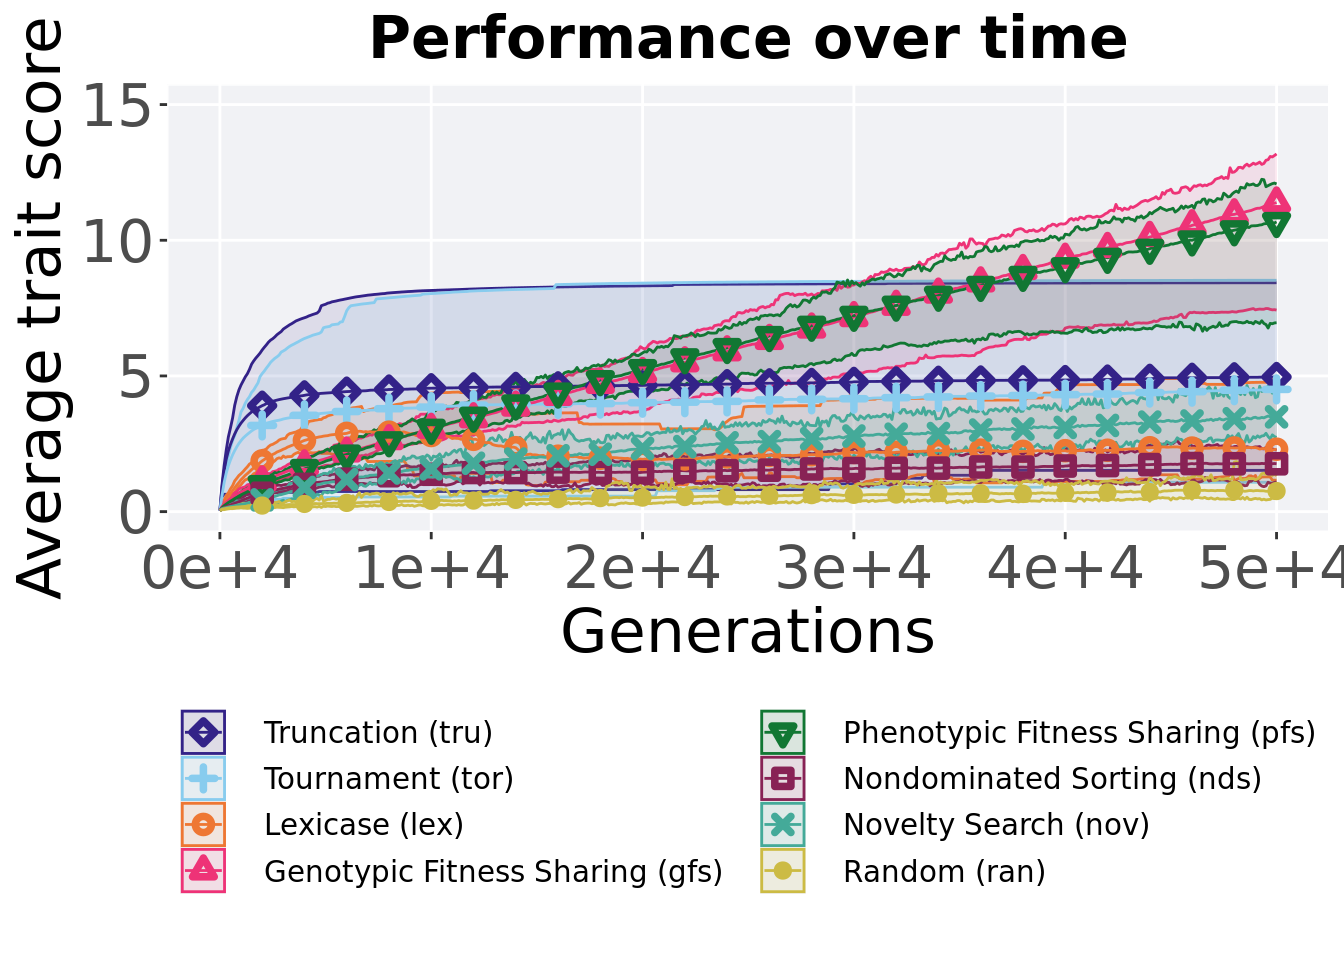
\includegraphics{demo_files/figure-latex/mpe-mvc-per-ot-1.pdf}

\hypertarget{best-performance-throughout-5}{%
\subsubsection{Best performance throughout}\label{best-performance-throughout-5}}

Best performance found throughout 50,000 generations.

\begin{Shaded}
\begin{Highlighting}[]
\CommentTok{### best performance throughout}
\KeywordTok{filter}\NormalTok{(cc_best_mvc, col }\OperatorTok{==}\StringTok{ 'pop_fit_max'} \OperatorTok{&}\StringTok{ }\NormalTok{diagnostic }\OperatorTok{==}\StringTok{ 'multipath_exploration'}\NormalTok{) }\OperatorTok
\StringTok{  }\KeywordTok{ggplot}\NormalTok{(., }\KeywordTok{aes}\NormalTok{(}\DataTypeTok{x =}\NormalTok{ acron, }\DataTypeTok{y =}\NormalTok{ val }\OperatorTok{/}\StringTok{ }\NormalTok{DIMENSIONALITY, }\DataTypeTok{color =}\NormalTok{ acron, }\DataTypeTok{fill =}\NormalTok{ acron, }\DataTypeTok{shape =}\NormalTok{ acron)) }\OperatorTok{+}
\StringTok{  }\KeywordTok{geom_flat_violin}\NormalTok{(}\DataTypeTok{position =} \KeywordTok{position_nudge}\NormalTok{(}\DataTypeTok{x =} \FloatTok{.2}\NormalTok{, }\DataTypeTok{y =} \DecValTok{0}\NormalTok{), }\DataTypeTok{scale =} \StringTok{'width'}\NormalTok{, }\DataTypeTok{alpha =} \FloatTok{0.2}\NormalTok{) }\OperatorTok{+}
\StringTok{  }\KeywordTok{geom_point}\NormalTok{(}\DataTypeTok{position =} \KeywordTok{position_jitter}\NormalTok{(}\DataTypeTok{width =} \FloatTok{.1}\NormalTok{), }\DataTypeTok{size =} \FloatTok{1.5}\NormalTok{, }\DataTypeTok{alpha =} \FloatTok{1.0}\NormalTok{) }\OperatorTok{+}
\StringTok{  }\KeywordTok{geom_boxplot}\NormalTok{(}\DataTypeTok{color =} \StringTok{'black'}\NormalTok{, }\DataTypeTok{width =} \FloatTok{.2}\NormalTok{, }\DataTypeTok{outlier.shape =} \OtherTok{NA}\NormalTok{, }\DataTypeTok{alpha =} \FloatTok{0.0}\NormalTok{) }\OperatorTok{+}
\StringTok{  }\KeywordTok{guides}\NormalTok{(}\DataTypeTok{fill =} \StringTok{"none"}\NormalTok{,}\DataTypeTok{color =} \StringTok{'none'}\NormalTok{, }\DataTypeTok{shape =} \StringTok{'none'}\NormalTok{) }\OperatorTok{+}
\StringTok{  }\KeywordTok{scale_y_continuous}\NormalTok{(}
    \DataTypeTok{name=}\StringTok{"Average trait score"}\NormalTok{,}
    \DataTypeTok{limits=}\KeywordTok{c}\NormalTok{(}\DecValTok{0}\NormalTok{, }\DecValTok{15}\NormalTok{),}
    \DataTypeTok{breaks=}\KeywordTok{seq}\NormalTok{(}\DecValTok{0}\NormalTok{,}\DecValTok{15}\NormalTok{, }\DecValTok{5}\NormalTok{),}
    \DataTypeTok{labels=}\KeywordTok{c}\NormalTok{(}\StringTok{"0"}\NormalTok{, }\StringTok{"5"}\NormalTok{, }\StringTok{"10"}\NormalTok{, }\StringTok{"15"}\NormalTok{)}
\NormalTok{  ) }\OperatorTok{+}
\StringTok{  }\KeywordTok{scale_x_discrete}\NormalTok{(}
    \DataTypeTok{name=}\StringTok{"Scheme"}
\NormalTok{  )}\OperatorTok{+}
\StringTok{  }\KeywordTok{scale_shape_manual}\NormalTok{(}\DataTypeTok{values=}\NormalTok{SHAPE)}\OperatorTok{+}
\StringTok{  }\KeywordTok{scale_colour_manual}\NormalTok{(}\DataTypeTok{values =}\NormalTok{ cb_palette, ) }\OperatorTok{+}
\StringTok{  }\KeywordTok{scale_fill_manual}\NormalTok{(}\DataTypeTok{values =}\NormalTok{ cb_palette) }\OperatorTok{+}
\StringTok{  }\KeywordTok{ggtitle}\NormalTok{(}\StringTok{'Best performance throughout'}\NormalTok{)}\OperatorTok{+}
\StringTok{  }\NormalTok{p_theme }\OperatorTok{+}\StringTok{ }\KeywordTok{theme}\NormalTok{(}\DataTypeTok{legend.title=}\KeywordTok{element_blank}\NormalTok{()) }\OperatorTok{+}
\StringTok{  }\KeywordTok{guides}\NormalTok{(}
    \DataTypeTok{shape=}\KeywordTok{guide_legend}\NormalTok{(}\DataTypeTok{nrow=}\DecValTok{2}\NormalTok{, }\DataTypeTok{title.position =} \StringTok{"bottom"}\NormalTok{),}
    \DataTypeTok{color=}\KeywordTok{guide_legend}\NormalTok{(}\DataTypeTok{nrow=}\DecValTok{2}\NormalTok{, }\DataTypeTok{title.position =} \StringTok{"bottom"}\NormalTok{),}
    \DataTypeTok{fill=}\KeywordTok{guide_legend}\NormalTok{(}\DataTypeTok{nrow=}\DecValTok{2}\NormalTok{, }\DataTypeTok{title.position =} \StringTok{"bottom"}\NormalTok{)}
\NormalTok{  )}
\end{Highlighting}
\end{Shaded}

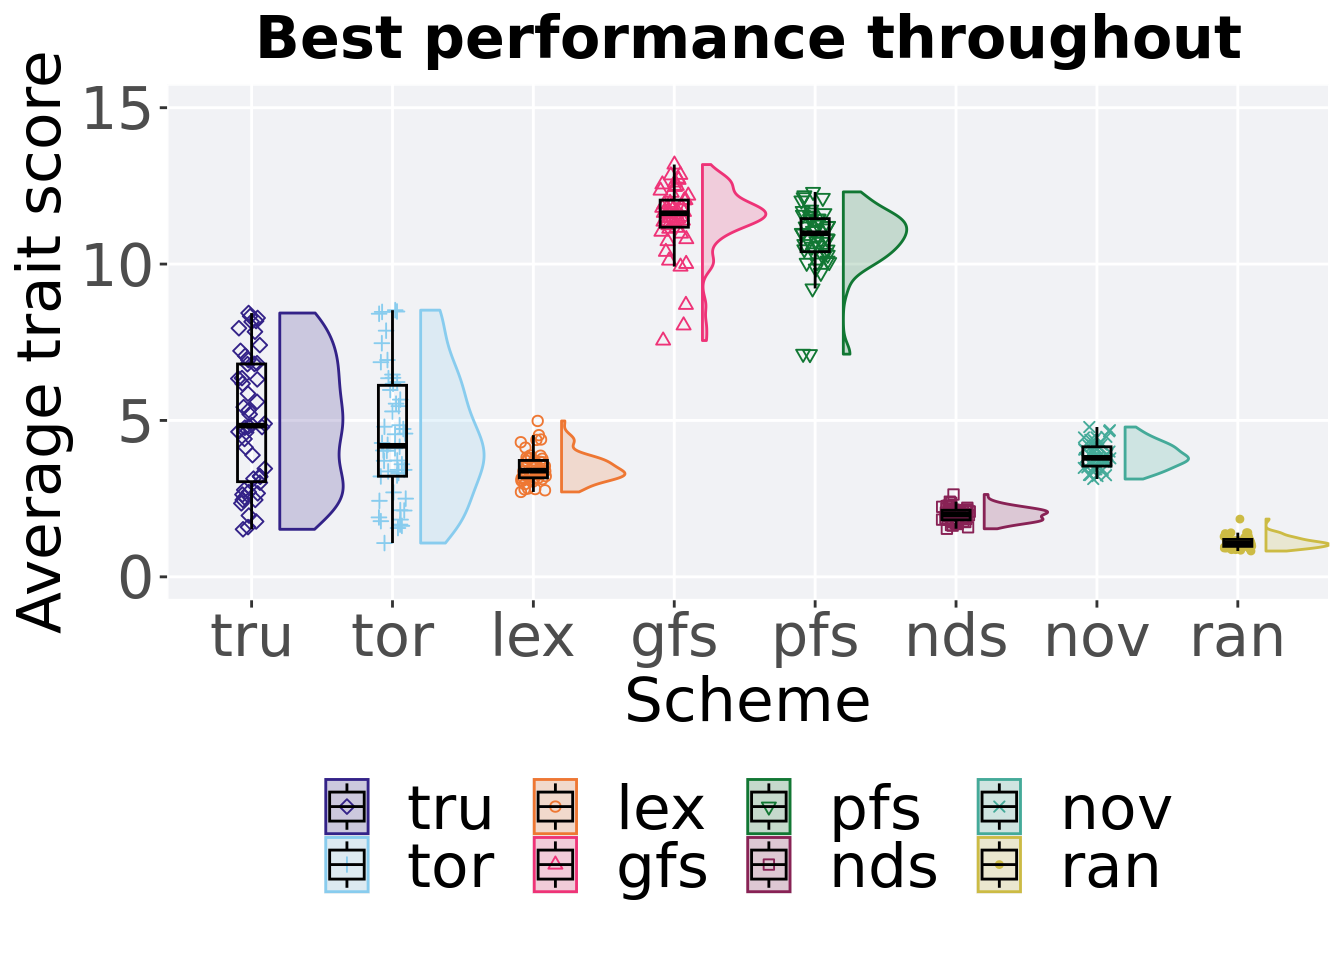
\includegraphics{demo_files/figure-latex/mpe-mvc-per-bst-1.pdf}

\hypertarget{stats-19}{%
\paragraph{Stats}\label{stats-19}}

Summary statistics for the performance of the best performance.

\begin{Shaded}
\begin{Highlighting}[]
\CommentTok{### best performance throughout}
\NormalTok{performance =}\StringTok{ }\KeywordTok{filter}\NormalTok{(cc_best_mvc, col }\OperatorTok{==}\StringTok{ 'pop_fit_max'} \OperatorTok{&}\StringTok{ }\NormalTok{diagnostic }\OperatorTok{==}\StringTok{ 'multipath_exploration'}\NormalTok{)}
\NormalTok{performance}\OperatorTok{$}\NormalTok{acron =}\StringTok{ }\KeywordTok{factor}\NormalTok{(performance}\OperatorTok{$}\NormalTok{acron, }\DataTypeTok{levels =} \KeywordTok{c}\NormalTok{(}\StringTok{'gfs'}\NormalTok{,}\StringTok{'pfs'}\NormalTok{,}\StringTok{'tor'}\NormalTok{,}\StringTok{'tru'}\NormalTok{,}\StringTok{'nov'}\NormalTok{,}\StringTok{'lex'}\NormalTok{,}\StringTok{'nds'}\NormalTok{,}\StringTok{'ran'}\NormalTok{))}
\NormalTok{performance }\OperatorTok
\StringTok{  }\KeywordTok{group_by}\NormalTok{(acron) }\OperatorTok
\StringTok{  }\NormalTok{dplyr}\OperatorTok{::}\KeywordTok{summarise}\NormalTok{(}
    \DataTypeTok{count =} \KeywordTok{n}\NormalTok{(),}
    \DataTypeTok{na_cnt =} \KeywordTok{sum}\NormalTok{(}\KeywordTok{is.na}\NormalTok{(val)),}
    \DataTypeTok{min =} \KeywordTok{min}\NormalTok{(val }\OperatorTok{/}\StringTok{ }\NormalTok{DIMENSIONALITY, }\DataTypeTok{na.rm =} \OtherTok{TRUE}\NormalTok{),}
    \DataTypeTok{median =} \KeywordTok{median}\NormalTok{(val }\OperatorTok{/}\StringTok{ }\NormalTok{DIMENSIONALITY, }\DataTypeTok{na.rm =} \OtherTok{TRUE}\NormalTok{),}
    \DataTypeTok{mean =} \KeywordTok{mean}\NormalTok{(val }\OperatorTok{/}\StringTok{ }\NormalTok{DIMENSIONALITY, }\DataTypeTok{na.rm =} \OtherTok{TRUE}\NormalTok{),}
    \DataTypeTok{max =} \KeywordTok{max}\NormalTok{(val }\OperatorTok{/}\StringTok{ }\NormalTok{DIMENSIONALITY, }\DataTypeTok{na.rm =} \OtherTok{TRUE}\NormalTok{),}
    \DataTypeTok{IQR =} \KeywordTok{IQR}\NormalTok{(val }\OperatorTok{/}\StringTok{ }\NormalTok{DIMENSIONALITY, }\DataTypeTok{na.rm =} \OtherTok{TRUE}\NormalTok{)}
\NormalTok{  )}
\end{Highlighting}
\end{Shaded}

\begin{verbatim}
## # A tibble: 8 x 8
##   acron count na_cnt   min median  mean   max   IQR
##   <fct> <int>  <int> <dbl>  <dbl> <dbl> <dbl> <dbl>
## 1 gfs      50      0 7.56   11.6  11.5  13.2  0.865
## 2 pfs      50      0 7.12   11.0  10.8  12.3  1.06 
## 3 tor      50      0 1.08    4.19  4.50  8.53 2.91 
## 4 tru      50      0 1.52    4.83  4.96  8.43 3.76 
## 5 nov      50      0 3.13    3.80  3.88  4.79 0.617
## 6 lex      50      0 2.71    3.39  3.48  4.98 0.555
## 7 nds      50      0 1.54    1.99  1.98  2.63 0.307
## 8 ran      50      0 0.825   1.07  1.10  1.85 0.222
\end{verbatim}

Kruskal--Wallis test provides evidence of statistical differences.

\begin{Shaded}
\begin{Highlighting}[]
\KeywordTok{kruskal.test}\NormalTok{(val }\OperatorTok{~}\StringTok{ }\NormalTok{acron, }\DataTypeTok{data =}\NormalTok{ performance)}
\end{Highlighting}
\end{Shaded}

\begin{verbatim}
## 
##  Kruskal-Wallis rank sum test
## 
## data:  val by acron
## Kruskal-Wallis chi-squared = 335.6, df = 7, p-value < 2.2e-16
\end{verbatim}

Results for post-hoc Wilcoxon rank-sum test with a Bonferroni correction.

\begin{Shaded}
\begin{Highlighting}[]
\KeywordTok{pairwise.wilcox.test}\NormalTok{(}\DataTypeTok{x =}\NormalTok{ performance}\OperatorTok{$}\NormalTok{val, }\DataTypeTok{g =}\NormalTok{ performance}\OperatorTok{$}\NormalTok{acron, }\DataTypeTok{p.adjust.method =} \StringTok{"bonferroni"}\NormalTok{,}
                     \DataTypeTok{paired =} \OtherTok{FALSE}\NormalTok{, }\DataTypeTok{conf.int =} \OtherTok{FALSE}\NormalTok{, }\DataTypeTok{alternative =} \StringTok{'l'}\NormalTok{)}
\end{Highlighting}
\end{Shaded}

\begin{verbatim}
## 
##  Pairwise comparisons using Wilcoxon rank sum test with continuity correction 
## 
## data:  performance$val and performance$acron 
## 
##     gfs     pfs     tor     tru     nov     lex     nds    
## pfs 0.00212 -       -       -       -       -       -      
## tor < 2e-16 < 2e-16 -       -       -       -       -      
## tru < 2e-16 2.9e-16 1.00000 -       -       -       -      
## nov < 2e-16 < 2e-16 1.00000 0.18480 -       -       -      
## lex < 2e-16 < 2e-16 0.08240 0.02364 0.00014 -       -      
## nds < 2e-16 < 2e-16 2.5e-09 1.7e-12 < 2e-16 < 2e-16 -      
## ran < 2e-16 < 2e-16 5.2e-16 < 2e-16 < 2e-16 < 2e-16 2.6e-16
## 
## P value adjustment method: bonferroni
\end{verbatim}

\hypertarget{performance-comparison-2}{%
\subsubsection{Performance comparison}\label{performance-comparison-2}}

Best performances in the population at 40,000 and 50,000 generations.

\begin{verbatim}
## Warning: The following aesthetics were dropped during statistical transformation:
## colour, shape
## i This can happen when ggplot fails to infer the correct grouping structure in
##   the data.
## i Did you forget to specify a `group` aesthetic or to convert a numerical
##   variable into a factor?
## The following aesthetics were dropped during statistical transformation:
## colour, shape
## i This can happen when ggplot fails to infer the correct grouping structure in
##   the data.
## i Did you forget to specify a `group` aesthetic or to convert a numerical
##   variable into a factor?
\end{verbatim}

\begin{Shaded}
\begin{Highlighting}[]
\CommentTok{# 80% and final generation comparison}
\NormalTok{end =}\StringTok{ }\KeywordTok{filter}\NormalTok{(cc_over_time_mvc, diagnostic }\OperatorTok{==}\StringTok{ 'multipath_exploration'} \OperatorTok{&}\StringTok{ }\NormalTok{gen }\OperatorTok{==}\StringTok{ }\DecValTok{50000} \OperatorTok{&}\StringTok{ }\NormalTok{acron }\OperatorTok{!=}\StringTok{ 'ran'}\NormalTok{)}
\NormalTok{end}\OperatorTok{$}\NormalTok{Generation <-}\StringTok{ }\KeywordTok{factor}\NormalTok{(end}\OperatorTok{$}\NormalTok{gen)}

\NormalTok{mid =}\StringTok{ }\KeywordTok{filter}\NormalTok{(cc_over_time_mvc, diagnostic }\OperatorTok{==}\StringTok{ 'multipath_exploration'} \OperatorTok{&}\StringTok{ }\NormalTok{gen }\OperatorTok{==}\StringTok{ }\DecValTok{40000} \OperatorTok{&}\StringTok{ }\NormalTok{acron }\OperatorTok{!=}\StringTok{ 'ran'}\NormalTok{)}
\NormalTok{mid}\OperatorTok{$}\NormalTok{Generation <-}\StringTok{ }\KeywordTok{factor}\NormalTok{(mid}\OperatorTok{$}\NormalTok{gen)}

\NormalTok{mvc_p =}\StringTok{ }\KeywordTok{ggplot}\NormalTok{(mid, }\KeywordTok{aes}\NormalTok{(}\DataTypeTok{x =}\NormalTok{ acron, }\DataTypeTok{y=}\NormalTok{pop_fit_max }\OperatorTok{/}\StringTok{ }\NormalTok{DIMENSIONALITY, }\DataTypeTok{group =}\NormalTok{ acron, }\DataTypeTok{shape =}\NormalTok{ Generation)) }\OperatorTok{+}
\StringTok{  }\KeywordTok{geom_point}\NormalTok{(}\DataTypeTok{col =}\NormalTok{ mvc_col[}\DecValTok{1}\NormalTok{] , }\DataTypeTok{position =} \KeywordTok{position_jitternudge}\NormalTok{(}\DataTypeTok{jitter.width =} \FloatTok{.03}\NormalTok{, }\DataTypeTok{nudge.x =} \FloatTok{-0.05}\NormalTok{), }\DataTypeTok{size =} \DecValTok{2}\NormalTok{, }\DataTypeTok{alpha =} \FloatTok{1.0}\NormalTok{) }\OperatorTok{+}
\StringTok{  }\KeywordTok{geom_boxplot}\NormalTok{(}\DataTypeTok{position =} \KeywordTok{position_nudge}\NormalTok{(}\DataTypeTok{x =} \FloatTok{-.15}\NormalTok{, }\DataTypeTok{y =} \DecValTok{0}\NormalTok{), }\DataTypeTok{lwd =} \FloatTok{0.7}\NormalTok{, }\DataTypeTok{col =}\NormalTok{ mvc_col[}\DecValTok{1}\NormalTok{], }\DataTypeTok{fill =}\NormalTok{ mvc_col[}\DecValTok{1}\NormalTok{], }\DataTypeTok{width =} \FloatTok{.1}\NormalTok{, }\DataTypeTok{outlier.shape =} \OtherTok{NA}\NormalTok{, }\DataTypeTok{alpha =} \FloatTok{0.0}\NormalTok{) }\OperatorTok{+}

\StringTok{  }\KeywordTok{geom_point}\NormalTok{(}\DataTypeTok{data =}\NormalTok{ end, }\KeywordTok{aes}\NormalTok{(}\DataTypeTok{x =}\NormalTok{ acron, }\DataTypeTok{y=}\NormalTok{pop_fit_max }\OperatorTok{/}\StringTok{ }\NormalTok{DIMENSIONALITY), }\DataTypeTok{col =}\NormalTok{ mvc_col[}\DecValTok{2}\NormalTok{], }\DataTypeTok{position =} \KeywordTok{position_jitternudge}\NormalTok{(}\DataTypeTok{jitter.width =} \FloatTok{.03}\NormalTok{, }\DataTypeTok{nudge.x =} \FloatTok{0.05}\NormalTok{), }\DataTypeTok{size =} \DecValTok{2}\NormalTok{, }\DataTypeTok{alpha =} \FloatTok{1.0}\NormalTok{) }\OperatorTok{+}
\StringTok{  }\KeywordTok{geom_boxplot}\NormalTok{(}\DataTypeTok{data =}\NormalTok{ end, }\KeywordTok{aes}\NormalTok{(}\DataTypeTok{x =}\NormalTok{ acron, }\DataTypeTok{y=}\NormalTok{pop_fit_max }\OperatorTok{/}\StringTok{ }\NormalTok{DIMENSIONALITY), }\DataTypeTok{position =} \KeywordTok{position_nudge}\NormalTok{(}\DataTypeTok{x =} \FloatTok{.15}\NormalTok{, }\DataTypeTok{y =} \DecValTok{0}\NormalTok{), }\DataTypeTok{lwd =} \FloatTok{0.7}\NormalTok{, }\DataTypeTok{col =}\NormalTok{ mvc_col[}\DecValTok{2}\NormalTok{], }\DataTypeTok{fill =}\NormalTok{ mvc_col[}\DecValTok{2}\NormalTok{], }\DataTypeTok{width =} \FloatTok{.1}\NormalTok{, }\DataTypeTok{outlier.shape =} \OtherTok{NA}\NormalTok{, }\DataTypeTok{alpha =} \FloatTok{0.0}\NormalTok{) }\OperatorTok{+}

\StringTok{  }\KeywordTok{scale_y_continuous}\NormalTok{(}
    \DataTypeTok{name=}\StringTok{"Average trait score"}\NormalTok{,}
    \DataTypeTok{limits=}\KeywordTok{c}\NormalTok{(}\DecValTok{0}\NormalTok{, }\DecValTok{15}\NormalTok{),}
    \DataTypeTok{breaks=}\KeywordTok{seq}\NormalTok{(}\DecValTok{0}\NormalTok{,}\DecValTok{15}\NormalTok{, }\DecValTok{5}\NormalTok{),}
    \DataTypeTok{labels=}\KeywordTok{c}\NormalTok{(}\StringTok{"0"}\NormalTok{, }\StringTok{"5"}\NormalTok{, }\StringTok{"10"}\NormalTok{, }\StringTok{"15"}\NormalTok{)}
\NormalTok{  ) }\OperatorTok{+}
\StringTok{  }\KeywordTok{scale_x_discrete}\NormalTok{(}
    \DataTypeTok{name=}\StringTok{"Scheme"}
\NormalTok{  )}\OperatorTok{+}
\StringTok{  }\KeywordTok{scale_shape_manual}\NormalTok{(}\DataTypeTok{values=}\KeywordTok{c}\NormalTok{(}\DecValTok{0}\NormalTok{,}\DecValTok{1}\NormalTok{))}\OperatorTok{+}
\StringTok{  }\KeywordTok{scale_colour_manual}\NormalTok{(}\DataTypeTok{values =} \KeywordTok{c}\NormalTok{(mvc_col[}\DecValTok{1}\NormalTok{],mvc_col[}\DecValTok{2}\NormalTok{])) }\OperatorTok{+}
\StringTok{  }\NormalTok{p_theme}

\KeywordTok{plot_grid}\NormalTok{(}
\NormalTok{  mvc_p }\OperatorTok{+}
\StringTok{    }\KeywordTok{ggtitle}\NormalTok{(}\StringTok{"Performance comparisons"}\NormalTok{) }\OperatorTok{+}
\StringTok{    }\KeywordTok{theme}\NormalTok{(}\DataTypeTok{legend.position=}\StringTok{"none"}\NormalTok{),}
\NormalTok{  legend,}
  \DataTypeTok{nrow=}\DecValTok{2}\NormalTok{,}
  \DataTypeTok{rel_heights =} \KeywordTok{c}\NormalTok{(}\DecValTok{1}\NormalTok{,.}\DecValTok{05}\NormalTok{),}
  \DataTypeTok{label_size =}\NormalTok{ TSIZE}
\NormalTok{)}
\end{Highlighting}
\end{Shaded}

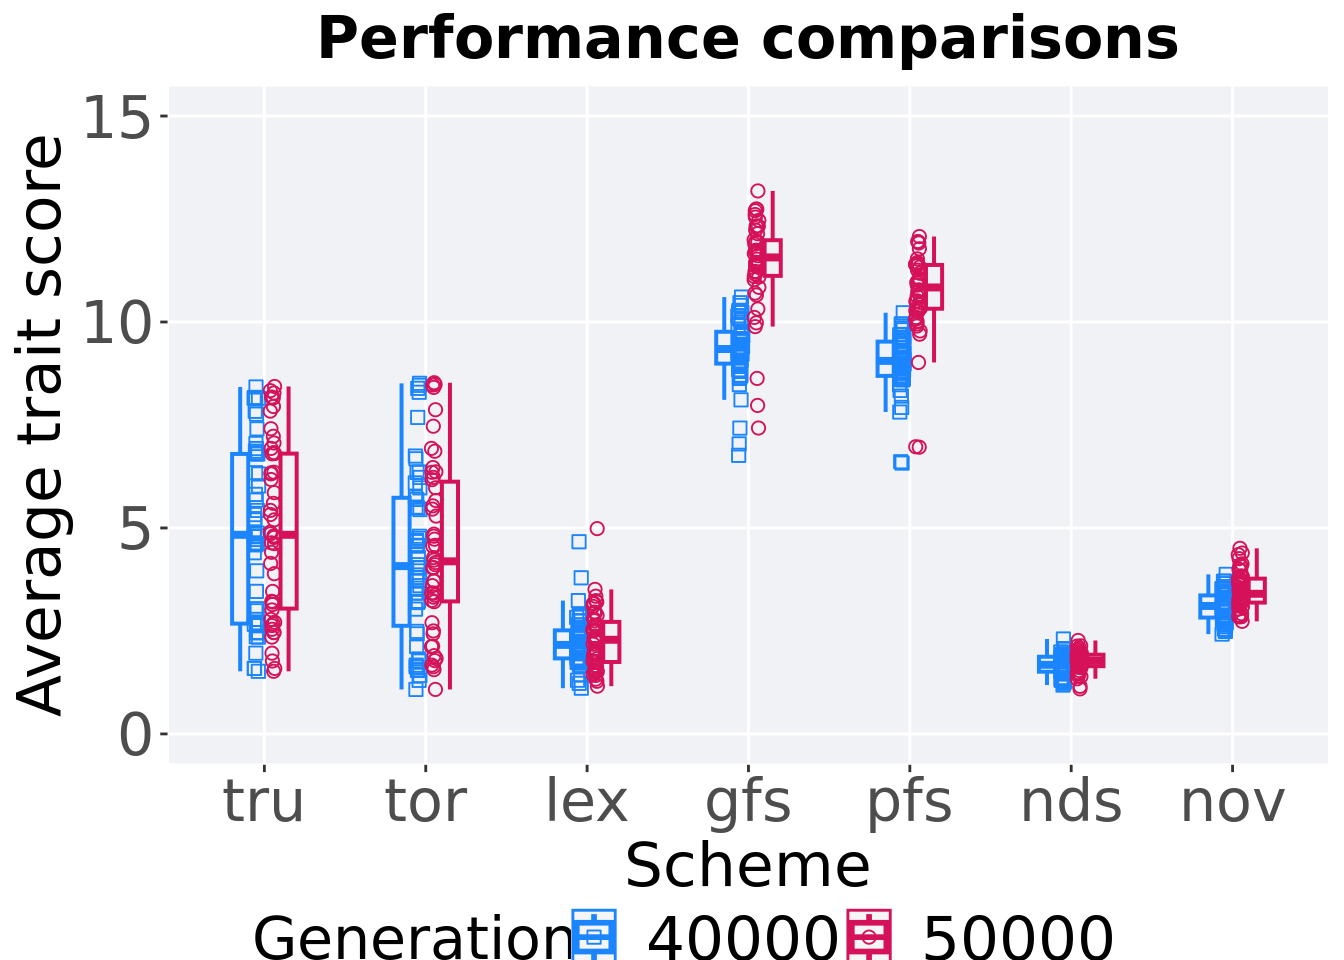
\includegraphics{demo_files/figure-latex/mpe-mvc-per-sli-1.pdf}

\hypertarget{stats-20}{%
\paragraph{Stats}\label{stats-20}}

Summary statistics for the performance of the best performance at 40,000 and 50,000 generations.

\begin{Shaded}
\begin{Highlighting}[]
\CommentTok{### performance comparisons and generation slices 40K & 50K}
\NormalTok{slices =}\StringTok{ }\KeywordTok{filter}\NormalTok{(cc_over_time_mvc, diagnostic }\OperatorTok{==}\StringTok{ 'multipath_exploration'} \OperatorTok{&}\StringTok{ }\NormalTok{(gen }\OperatorTok{==}\StringTok{ }\DecValTok{50000} \OperatorTok{|}\StringTok{ }\NormalTok{gen }\OperatorTok{==}\StringTok{ }\DecValTok{40000}\NormalTok{) }\OperatorTok{&}\StringTok{ }\NormalTok{acron }\OperatorTok{!=}\StringTok{ 'ran'}\NormalTok{)}
\NormalTok{slices}\OperatorTok{$}\NormalTok{Generation <-}\StringTok{ }\KeywordTok{factor}\NormalTok{(slices}\OperatorTok{$}\NormalTok{gen, }\DataTypeTok{levels =} \KeywordTok{c}\NormalTok{(}\DecValTok{50000}\NormalTok{,}\DecValTok{40000}\NormalTok{))}
\NormalTok{slices}\OperatorTok{$}\NormalTok{acron =}\StringTok{ }\KeywordTok{factor}\NormalTok{(slices}\OperatorTok{$}\NormalTok{acron, }\DataTypeTok{levels =} \KeywordTok{c}\NormalTok{(}\StringTok{'gfs'}\NormalTok{,}\StringTok{'pfs'}\NormalTok{,}\StringTok{'tru'}\NormalTok{,}\StringTok{'tor'}\NormalTok{,}\StringTok{'nov'}\NormalTok{, }\StringTok{'nds'}\NormalTok{,}\StringTok{'lex'}\NormalTok{, }\StringTok{'ran'}\NormalTok{))}
\NormalTok{slices }\OperatorTok
\StringTok{  }\KeywordTok{group_by}\NormalTok{(acron, Generation) }\OperatorTok
\StringTok{  }\NormalTok{dplyr}\OperatorTok{::}\KeywordTok{summarise}\NormalTok{(}
    \DataTypeTok{count =} \KeywordTok{n}\NormalTok{(),}
    \DataTypeTok{na_cnt =} \KeywordTok{sum}\NormalTok{(}\KeywordTok{is.na}\NormalTok{(pop_fit_max  }\OperatorTok{/}\StringTok{ }\NormalTok{DIMENSIONALITY)),}
    \DataTypeTok{min =} \KeywordTok{min}\NormalTok{(pop_fit_max  }\OperatorTok{/}\StringTok{ }\NormalTok{DIMENSIONALITY, }\DataTypeTok{na.rm =} \OtherTok{TRUE}\NormalTok{),}
    \DataTypeTok{median =} \KeywordTok{median}\NormalTok{(pop_fit_max  }\OperatorTok{/}\StringTok{ }\NormalTok{DIMENSIONALITY, }\DataTypeTok{na.rm =} \OtherTok{TRUE}\NormalTok{),}
    \DataTypeTok{mean =} \KeywordTok{mean}\NormalTok{(pop_fit_max  }\OperatorTok{/}\StringTok{ }\NormalTok{DIMENSIONALITY, }\DataTypeTok{na.rm =} \OtherTok{TRUE}\NormalTok{),}
    \DataTypeTok{max =} \KeywordTok{max}\NormalTok{(pop_fit_max  }\OperatorTok{/}\StringTok{ }\NormalTok{DIMENSIONALITY, }\DataTypeTok{na.rm =} \OtherTok{TRUE}\NormalTok{),}
    \DataTypeTok{IQR =} \KeywordTok{IQR}\NormalTok{(pop_fit_max  }\OperatorTok{/}\StringTok{ }\NormalTok{DIMENSIONALITY, }\DataTypeTok{na.rm =} \OtherTok{TRUE}\NormalTok{)}
\NormalTok{  )}
\end{Highlighting}
\end{Shaded}

\begin{verbatim}
## `summarise()` has grouped output by 'acron'. You can override using the
## `.groups` argument.
\end{verbatim}

\begin{verbatim}
## # A tibble: 14 x 9
## # Groups:   acron [7]
##    acron Generation count na_cnt   min median  mean   max   IQR
##    <fct> <fct>      <int>  <int> <dbl>  <dbl> <dbl> <dbl> <dbl>
##  1 gfs   50000         50      0  7.43  11.6  11.4  13.2  0.865
##  2 gfs   40000         50      0  6.76   9.34  9.32 10.6  0.772
##  3 pfs   50000         50      0  6.96  10.8  10.7  12.1  1.06 
##  4 pfs   40000         50      0  6.57   9.06  9.01 10.2  0.832
##  5 tru   50000         50      0  1.52   4.83  4.96  8.43 3.76 
##  6 tru   40000         50      0  1.52   4.83  4.85  8.42 4.12 
##  7 tor   50000         50      0  1.08   4.19  4.50  8.53 2.91 
##  8 tor   40000         50      0  1.08   4.07  4.31  8.51 3.11 
##  9 nov   50000         50      0  2.73   3.40  3.49  4.51 0.582
## 10 nov   40000         50      0  2.42   3.11  3.10  3.87 0.538
## 11 nds   50000         50      0  1.09   1.78  1.76  2.27 0.279
## 12 nds   40000         50      0  1.19   1.68  1.68  2.30 0.363
## 13 lex   50000         50      0  1.16   2.29  2.30  4.98 0.974
## 14 lex   40000         50      0  1.11   2.16  2.25  4.67 0.681
\end{verbatim}

Truncation selection comparisons.

\begin{Shaded}
\begin{Highlighting}[]
\KeywordTok{wilcox.test}\NormalTok{(}\DataTypeTok{x =} \KeywordTok{filter}\NormalTok{(slices, acron }\OperatorTok{==}\StringTok{ 'tru'} \OperatorTok{&}\StringTok{ }\NormalTok{Generation }\OperatorTok{==}\StringTok{ }\DecValTok{50000}\NormalTok{)}\OperatorTok{$}\NormalTok{pop_fit_max,}
            \DataTypeTok{y =} \KeywordTok{filter}\NormalTok{(slices, acron }\OperatorTok{==}\StringTok{ 'tru'} \OperatorTok{&}\StringTok{ }\NormalTok{Generation }\OperatorTok{==}\StringTok{ }\DecValTok{40000}\NormalTok{)}\OperatorTok{$}\NormalTok{pop_fit_max,}
            \DataTypeTok{alternative =} \StringTok{'t'}\NormalTok{)}
\end{Highlighting}
\end{Shaded}

\begin{verbatim}
## 
##  Wilcoxon rank sum test with continuity correction
## 
## data:  filter(slices, acron == "tru" & Generation == 50000)$pop_fit_max and filter(slices, acron == "tru" & Generation == 40000)$pop_fit_max
## W = 1317, p-value = 0.6466
## alternative hypothesis: true location shift is not equal to 0
\end{verbatim}

Tournament selection comparisons.

\begin{Shaded}
\begin{Highlighting}[]
\KeywordTok{wilcox.test}\NormalTok{(}\DataTypeTok{x =} \KeywordTok{filter}\NormalTok{(slices, acron }\OperatorTok{==}\StringTok{ 'tor'} \OperatorTok{&}\StringTok{ }\NormalTok{Generation }\OperatorTok{==}\StringTok{ }\DecValTok{50000}\NormalTok{)}\OperatorTok{$}\NormalTok{pop_fit_max,}
            \DataTypeTok{y =} \KeywordTok{filter}\NormalTok{(slices, acron }\OperatorTok{==}\StringTok{ 'tor'} \OperatorTok{&}\StringTok{ }\NormalTok{Generation }\OperatorTok{==}\StringTok{ }\DecValTok{40000}\NormalTok{)}\OperatorTok{$}\NormalTok{pop_fit_max,}
            \DataTypeTok{alternative =} \StringTok{'t'}\NormalTok{)}
\end{Highlighting}
\end{Shaded}

\begin{verbatim}
## 
##  Wilcoxon rank sum test with continuity correction
## 
## data:  filter(slices, acron == "tor" & Generation == 50000)$pop_fit_max and filter(slices, acron == "tor" & Generation == 40000)$pop_fit_max
## W = 1339, p-value = 0.5418
## alternative hypothesis: true location shift is not equal to 0
\end{verbatim}

Lexicase selection comparisons.

\begin{Shaded}
\begin{Highlighting}[]
\KeywordTok{wilcox.test}\NormalTok{(}\DataTypeTok{x =} \KeywordTok{filter}\NormalTok{(slices, acron }\OperatorTok{==}\StringTok{ 'lex'} \OperatorTok{&}\StringTok{ }\NormalTok{Generation }\OperatorTok{==}\StringTok{ }\DecValTok{50000}\NormalTok{)}\OperatorTok{$}\NormalTok{pop_fit_max,}
            \DataTypeTok{y =} \KeywordTok{filter}\NormalTok{(slices, acron }\OperatorTok{==}\StringTok{ 'lex'} \OperatorTok{&}\StringTok{ }\NormalTok{Generation }\OperatorTok{==}\StringTok{ }\DecValTok{40000}\NormalTok{)}\OperatorTok{$}\NormalTok{pop_fit_max,}
            \DataTypeTok{alternative =} \StringTok{'t'}\NormalTok{)}
\end{Highlighting}
\end{Shaded}

\begin{verbatim}
## 
##  Wilcoxon rank sum test with continuity correction
## 
## data:  filter(slices, acron == "lex" & Generation == 50000)$pop_fit_max and filter(slices, acron == "lex" & Generation == 40000)$pop_fit_max
## W = 1286, p-value = 0.8067
## alternative hypothesis: true location shift is not equal to 0
\end{verbatim}

Genotypic fitness sharing comparisons.

\begin{Shaded}
\begin{Highlighting}[]
\KeywordTok{wilcox.test}\NormalTok{(}\DataTypeTok{x =} \KeywordTok{filter}\NormalTok{(slices, acron }\OperatorTok{==}\StringTok{ 'gfs'} \OperatorTok{&}\StringTok{ }\NormalTok{Generation }\OperatorTok{==}\StringTok{ }\DecValTok{50000}\NormalTok{)}\OperatorTok{$}\NormalTok{pop_fit_max,}
            \DataTypeTok{y =} \KeywordTok{filter}\NormalTok{(slices, acron }\OperatorTok{==}\StringTok{ 'gfs'} \OperatorTok{&}\StringTok{ }\NormalTok{Generation }\OperatorTok{==}\StringTok{ }\DecValTok{40000}\NormalTok{)}\OperatorTok{$}\NormalTok{pop_fit_max,}
            \DataTypeTok{alternative =} \StringTok{'t'}\NormalTok{)}
\end{Highlighting}
\end{Shaded}

\begin{verbatim}
## 
##  Wilcoxon rank sum test with continuity correction
## 
## data:  filter(slices, acron == "gfs" & Generation == 50000)$pop_fit_max and filter(slices, acron == "gfs" & Generation == 40000)$pop_fit_max
## W = 2327, p-value = 1.161e-13
## alternative hypothesis: true location shift is not equal to 0
\end{verbatim}

Phenotypic fitness sharing comparisons.

\begin{Shaded}
\begin{Highlighting}[]
\KeywordTok{wilcox.test}\NormalTok{(}\DataTypeTok{x =} \KeywordTok{filter}\NormalTok{(slices, acron }\OperatorTok{==}\StringTok{ 'pfs'} \OperatorTok{&}\StringTok{ }\NormalTok{Generation }\OperatorTok{==}\StringTok{ }\DecValTok{50000}\NormalTok{)}\OperatorTok{$}\NormalTok{pop_fit_max,}
            \DataTypeTok{y =} \KeywordTok{filter}\NormalTok{(slices, acron }\OperatorTok{==}\StringTok{ 'pfs'} \OperatorTok{&}\StringTok{ }\NormalTok{Generation }\OperatorTok{==}\StringTok{ }\DecValTok{40000}\NormalTok{)}\OperatorTok{$}\NormalTok{pop_fit_max,}
            \DataTypeTok{alternative =} \StringTok{'t'}\NormalTok{)}
\end{Highlighting}
\end{Shaded}

\begin{verbatim}
## 
##  Wilcoxon rank sum test with continuity correction
## 
## data:  filter(slices, acron == "pfs" & Generation == 50000)$pop_fit_max and filter(slices, acron == "pfs" & Generation == 40000)$pop_fit_max
## W = 2358, p-value = 2.26e-14
## alternative hypothesis: true location shift is not equal to 0
\end{verbatim}

Nondominated sorting comparisons.

\begin{Shaded}
\begin{Highlighting}[]
\KeywordTok{wilcox.test}\NormalTok{(}\DataTypeTok{x =} \KeywordTok{filter}\NormalTok{(slices, acron }\OperatorTok{==}\StringTok{ 'nds'} \OperatorTok{&}\StringTok{ }\NormalTok{Generation }\OperatorTok{==}\StringTok{ }\DecValTok{50000}\NormalTok{)}\OperatorTok{$}\NormalTok{pop_fit_max,}
            \DataTypeTok{y =} \KeywordTok{filter}\NormalTok{(slices, acron }\OperatorTok{==}\StringTok{ 'nds'} \OperatorTok{&}\StringTok{ }\NormalTok{Generation }\OperatorTok{==}\StringTok{ }\DecValTok{40000}\NormalTok{)}\OperatorTok{$}\NormalTok{pop_fit_max,}
            \DataTypeTok{alternative =} \StringTok{'t'}\NormalTok{)}
\end{Highlighting}
\end{Shaded}

\begin{verbatim}
## 
##  Wilcoxon rank sum test with continuity correction
## 
## data:  filter(slices, acron == "nds" & Generation == 50000)$pop_fit_max and filter(slices, acron == "nds" & Generation == 40000)$pop_fit_max
## W = 1509, p-value = 0.07474
## alternative hypothesis: true location shift is not equal to 0
\end{verbatim}

Novelty search comparisons.

\begin{Shaded}
\begin{Highlighting}[]
\KeywordTok{wilcox.test}\NormalTok{(}\DataTypeTok{x =} \KeywordTok{filter}\NormalTok{(slices, acron }\OperatorTok{==}\StringTok{ 'nov'} \OperatorTok{&}\StringTok{ }\NormalTok{Generation }\OperatorTok{==}\StringTok{ }\DecValTok{50000}\NormalTok{)}\OperatorTok{$}\NormalTok{pop_fit_max,}
            \DataTypeTok{y =} \KeywordTok{filter}\NormalTok{(slices, acron }\OperatorTok{==}\StringTok{ 'nov'} \OperatorTok{&}\StringTok{ }\NormalTok{Generation }\OperatorTok{==}\StringTok{ }\DecValTok{40000}\NormalTok{)}\OperatorTok{$}\NormalTok{pop_fit_max,}
            \DataTypeTok{alternative =} \StringTok{'t'}\NormalTok{)}
\end{Highlighting}
\end{Shaded}

\begin{verbatim}
## 
##  Wilcoxon rank sum test with continuity correction
## 
## data:  filter(slices, acron == "nov" & Generation == 50000)$pop_fit_max and filter(slices, acron == "nov" & Generation == 40000)$pop_fit_max
## W = 1872, p-value = 1.831e-05
## alternative hypothesis: true location shift is not equal to 0
\end{verbatim}

\hypertarget{activation-gene-coverage-3}{%
\subsection{Activation gene coverage}\label{activation-gene-coverage-3}}

Activation gene coverage analysis.

\hypertarget{coverage-over-time-4}{%
\subsubsection{Coverage over time}\label{coverage-over-time-4}}

Activation gene coverage over time.

\begin{Shaded}
\begin{Highlighting}[]
\CommentTok{# data for lines and shading on plots}
\NormalTok{lines =}\StringTok{ }\KeywordTok{filter}\NormalTok{(cc_over_time_mvc, diagnostic }\OperatorTok{==}\StringTok{ 'multipath_exploration'}\NormalTok{) }\OperatorTok
\StringTok{  }\KeywordTok{group_by}\NormalTok{(}\StringTok{`}\DataTypeTok{Selection}\CharTok{\textbackslash{}n}\DataTypeTok{Scheme}\StringTok{`}\NormalTok{, gen) }\OperatorTok
\StringTok{  }\NormalTok{dplyr}\OperatorTok{::}\KeywordTok{summarise}\NormalTok{(}
    \DataTypeTok{min =} \KeywordTok{min}\NormalTok{(uni_str_pos),}
    \DataTypeTok{mean =} \KeywordTok{mean}\NormalTok{(uni_str_pos),}
    \DataTypeTok{max =} \KeywordTok{max}\NormalTok{(uni_str_pos)}
\NormalTok{  )}
\end{Highlighting}
\end{Shaded}

\begin{verbatim}
## `summarise()` has grouped output by 'Selection Scheme'. You can override using
## the `.groups` argument.
\end{verbatim}

\begin{Shaded}
\begin{Highlighting}[]
\KeywordTok{ggplot}\NormalTok{(lines, }\KeywordTok{aes}\NormalTok{(}\DataTypeTok{x=}\NormalTok{gen, }\DataTypeTok{y=}\NormalTok{mean, }\DataTypeTok{group =} \StringTok{`}\DataTypeTok{Selection}\CharTok{\textbackslash{}n}\DataTypeTok{Scheme}\StringTok{`}\NormalTok{, }\DataTypeTok{fill =}\StringTok{`}\DataTypeTok{Selection}\CharTok{\textbackslash{}n}\DataTypeTok{Scheme}\StringTok{`}\NormalTok{, }\DataTypeTok{color =} \StringTok{`}\DataTypeTok{Selection}\CharTok{\textbackslash{}n}\DataTypeTok{Scheme}\StringTok{`}\NormalTok{, }\DataTypeTok{shape =} \StringTok{`}\DataTypeTok{Selection}\CharTok{\textbackslash{}n}\DataTypeTok{Scheme}\StringTok{`}\NormalTok{)) }\OperatorTok{+}
\StringTok{  }\KeywordTok{geom_ribbon}\NormalTok{(}\KeywordTok{aes}\NormalTok{(}\DataTypeTok{ymin =}\NormalTok{ min, }\DataTypeTok{ymax =}\NormalTok{ max), }\DataTypeTok{alpha =} \FloatTok{0.1}\NormalTok{) }\OperatorTok{+}
\StringTok{  }\KeywordTok{geom_line}\NormalTok{(}\DataTypeTok{size =} \FloatTok{0.5}\NormalTok{) }\OperatorTok{+}
\StringTok{  }\KeywordTok{geom_point}\NormalTok{(}\DataTypeTok{data =} \KeywordTok{filter}\NormalTok{(lines, gen }\OperatorTok\StringTok{ }\DecValTok{2000} \OperatorTok{==}\StringTok{ }\DecValTok{0} \OperatorTok{&}\StringTok{ }\NormalTok{gen }\OperatorTok{!=}\StringTok{ }\DecValTok{0}\NormalTok{), }\DataTypeTok{size =} \FloatTok{1.5}\NormalTok{, }\DataTypeTok{stroke =} \FloatTok{2.0}\NormalTok{, }\DataTypeTok{alpha =} \FloatTok{1.0}\NormalTok{) }\OperatorTok{+}
\StringTok{  }\KeywordTok{scale_y_continuous}\NormalTok{(}
    \DataTypeTok{name=}\StringTok{"Coverage"}\NormalTok{,}
    \DataTypeTok{limits=}\KeywordTok{c}\NormalTok{(}\DecValTok{0}\NormalTok{, }\DecValTok{100}\NormalTok{),}
    \DataTypeTok{breaks=}\KeywordTok{seq}\NormalTok{(}\DecValTok{0}\NormalTok{,}\DecValTok{100}\NormalTok{, }\DecValTok{20}\NormalTok{),}
    \DataTypeTok{labels=}\KeywordTok{c}\NormalTok{(}\StringTok{"0"}\NormalTok{, }\StringTok{"20"}\NormalTok{, }\StringTok{"40"}\NormalTok{, }\StringTok{"60"}\NormalTok{, }\StringTok{"80"}\NormalTok{, }\StringTok{"100"}\NormalTok{)}
\NormalTok{  ) }\OperatorTok{+}
\StringTok{  }\KeywordTok{scale_x_continuous}\NormalTok{(}
    \DataTypeTok{name=}\StringTok{"Generations"}\NormalTok{,}
    \DataTypeTok{limits=}\KeywordTok{c}\NormalTok{(}\DecValTok{0}\NormalTok{, }\DecValTok{50000}\NormalTok{),}
    \DataTypeTok{breaks=}\KeywordTok{c}\NormalTok{(}\DecValTok{0}\NormalTok{, }\DecValTok{10000}\NormalTok{, }\DecValTok{20000}\NormalTok{, }\DecValTok{30000}\NormalTok{, }\DecValTok{40000}\NormalTok{, }\DecValTok{50000}\NormalTok{),}
    \DataTypeTok{labels=}\KeywordTok{c}\NormalTok{(}\StringTok{"0e+4"}\NormalTok{, }\StringTok{"1e+4"}\NormalTok{, }\StringTok{"2e+4"}\NormalTok{, }\StringTok{"3e+4"}\NormalTok{, }\StringTok{"4e+4"}\NormalTok{, }\StringTok{"5e+4"}\NormalTok{)}
\NormalTok{  ) }\OperatorTok{+}
\StringTok{  }\KeywordTok{scale_shape_manual}\NormalTok{(}\DataTypeTok{values=}\NormalTok{SHAPE)}\OperatorTok{+}
\StringTok{  }\KeywordTok{scale_colour_manual}\NormalTok{(}\DataTypeTok{values =}\NormalTok{ cb_palette) }\OperatorTok{+}
\StringTok{  }\KeywordTok{scale_fill_manual}\NormalTok{(}\DataTypeTok{values =}\NormalTok{ cb_palette) }\OperatorTok{+}
\StringTok{  }\KeywordTok{ggtitle}\NormalTok{(}\StringTok{'Activation gene coverage over time'}\NormalTok{)}\OperatorTok{+}
\StringTok{  }\NormalTok{p_theme }\OperatorTok{+}\StringTok{ }\KeywordTok{theme}\NormalTok{(}\DataTypeTok{legend.title=}\KeywordTok{element_blank}\NormalTok{(),}\DataTypeTok{legend.text=}\KeywordTok{element_text}\NormalTok{(}\DataTypeTok{size=}\DecValTok{11}\NormalTok{)) }\OperatorTok{+}
\StringTok{  }\KeywordTok{guides}\NormalTok{(}
    \DataTypeTok{shape=}\KeywordTok{guide_legend}\NormalTok{(}\DataTypeTok{ncol=}\DecValTok{2}\NormalTok{, }\DataTypeTok{title.position =} \StringTok{"bottom"}\NormalTok{),}
    \DataTypeTok{color=}\KeywordTok{guide_legend}\NormalTok{(}\DataTypeTok{ncol=}\DecValTok{2}\NormalTok{, }\DataTypeTok{title.position =} \StringTok{"bottom"}\NormalTok{),}
    \DataTypeTok{fill=}\KeywordTok{guide_legend}\NormalTok{(}\DataTypeTok{ncol=}\DecValTok{2}\NormalTok{, }\DataTypeTok{title.position =} \StringTok{"bottom"}\NormalTok{)}
\NormalTok{  )}
\end{Highlighting}
\end{Shaded}

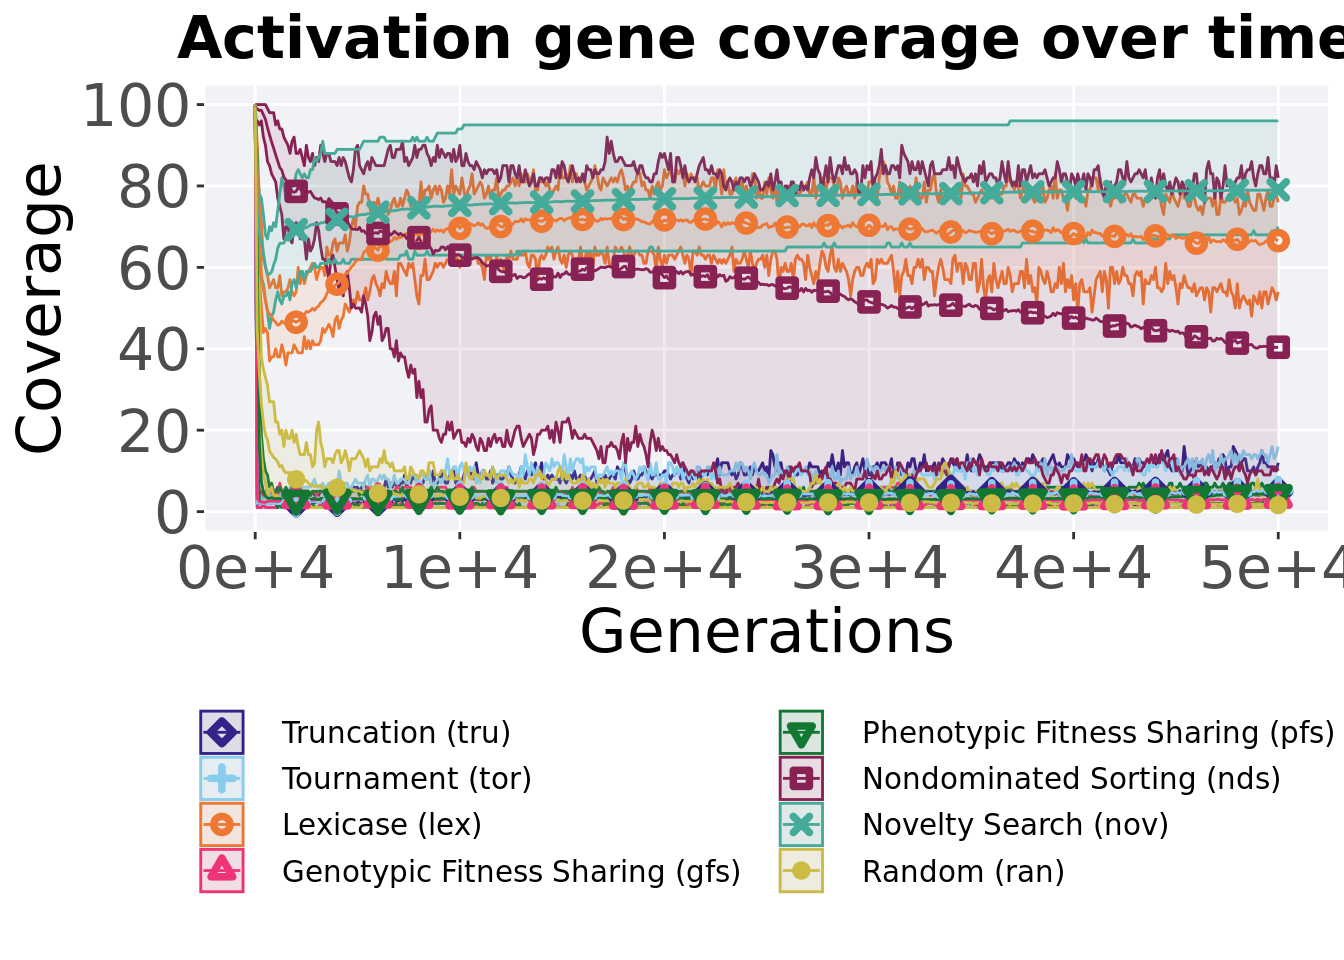
\includegraphics{demo_files/figure-latex/mpe-mvc-act-ot-1.pdf}

\hypertarget{coverage-comparison-2}{%
\subsubsection{Coverage comparison}\label{coverage-comparison-2}}

Best activation gene coverage in the population at 40,000 and 50,000 generations.

\begin{Shaded}
\begin{Highlighting}[]
\CommentTok{# 80% and final generation comparison}
\NormalTok{end =}\StringTok{ }\KeywordTok{filter}\NormalTok{(cc_over_time_mvc, diagnostic }\OperatorTok{==}\StringTok{ 'multipath_exploration'} \OperatorTok{&}\StringTok{ }\NormalTok{gen }\OperatorTok{==}\StringTok{ }\DecValTok{50000} \OperatorTok{&}\StringTok{ }\NormalTok{acron }\OperatorTok{!=}\StringTok{ 'ran'}\NormalTok{)}
\NormalTok{end}\OperatorTok{$}\NormalTok{Generation <-}\StringTok{ }\KeywordTok{factor}\NormalTok{(end}\OperatorTok{$}\NormalTok{gen)}

\NormalTok{mid =}\StringTok{ }\KeywordTok{filter}\NormalTok{(cc_over_time_mvc, diagnostic }\OperatorTok{==}\StringTok{ 'multipath_exploration'} \OperatorTok{&}\StringTok{ }\NormalTok{gen }\OperatorTok{==}\StringTok{ }\DecValTok{40000} \OperatorTok{&}\StringTok{ }\NormalTok{acron }\OperatorTok{!=}\StringTok{ 'ran'}\NormalTok{)}
\NormalTok{mid}\OperatorTok{$}\NormalTok{Generation <-}\StringTok{ }\KeywordTok{factor}\NormalTok{(mid}\OperatorTok{$}\NormalTok{gen)}

\NormalTok{mvc_p =}\StringTok{ }\KeywordTok{ggplot}\NormalTok{(mid, }\KeywordTok{aes}\NormalTok{(}\DataTypeTok{x =}\NormalTok{ acron, }\DataTypeTok{y=}\NormalTok{uni_str_pos, }\DataTypeTok{group =}\NormalTok{ acron, }\DataTypeTok{shape =}\NormalTok{ Generation)) }\OperatorTok{+}
\StringTok{  }\KeywordTok{geom_point}\NormalTok{(}\DataTypeTok{col =}\NormalTok{ mvc_col[}\DecValTok{1}\NormalTok{] , }\DataTypeTok{position =} \KeywordTok{position_jitternudge}\NormalTok{(}\DataTypeTok{jitter.width =} \FloatTok{.03}\NormalTok{, }\DataTypeTok{nudge.x =} \FloatTok{-0.05}\NormalTok{), }\DataTypeTok{size =} \DecValTok{2}\NormalTok{, }\DataTypeTok{alpha =} \FloatTok{1.0}\NormalTok{) }\OperatorTok{+}
\StringTok{  }\KeywordTok{geom_boxplot}\NormalTok{(}\DataTypeTok{position =} \KeywordTok{position_nudge}\NormalTok{(}\DataTypeTok{x =} \FloatTok{-.17}\NormalTok{, }\DataTypeTok{y =} \DecValTok{0}\NormalTok{), }\DataTypeTok{lwd =} \FloatTok{0.7}\NormalTok{, }\DataTypeTok{col =}\NormalTok{ mvc_col[}\DecValTok{1}\NormalTok{], }\DataTypeTok{fill =}\NormalTok{ mvc_col[}\DecValTok{1}\NormalTok{], }\DataTypeTok{width =} \FloatTok{.1}\NormalTok{, }\DataTypeTok{outlier.shape =} \OtherTok{NA}\NormalTok{, }\DataTypeTok{alpha =} \FloatTok{0.0}\NormalTok{) }\OperatorTok{+}

\StringTok{  }\KeywordTok{geom_point}\NormalTok{(}\DataTypeTok{data =}\NormalTok{ end, }\KeywordTok{aes}\NormalTok{(}\DataTypeTok{x =}\NormalTok{ acron, }\DataTypeTok{y=}\NormalTok{uni_str_pos), }\DataTypeTok{col =}\NormalTok{ mvc_col[}\DecValTok{2}\NormalTok{], }\DataTypeTok{position =} \KeywordTok{position_jitternudge}\NormalTok{(}\DataTypeTok{jitter.width =} \FloatTok{.03}\NormalTok{, }\DataTypeTok{nudge.x =} \FloatTok{0.05}\NormalTok{), }\DataTypeTok{size =} \DecValTok{2}\NormalTok{, }\DataTypeTok{alpha =} \FloatTok{1.0}\NormalTok{) }\OperatorTok{+}
\StringTok{  }\KeywordTok{geom_boxplot}\NormalTok{(}\DataTypeTok{data =}\NormalTok{ end, }\KeywordTok{aes}\NormalTok{(}\DataTypeTok{x =}\NormalTok{ acron, }\DataTypeTok{y=}\NormalTok{uni_str_pos), }\DataTypeTok{position =} \KeywordTok{position_nudge}\NormalTok{(}\DataTypeTok{x =} \FloatTok{.17}\NormalTok{, }\DataTypeTok{y =} \DecValTok{0}\NormalTok{), }\DataTypeTok{lwd =} \FloatTok{0.7}\NormalTok{, }\DataTypeTok{col =}\NormalTok{ mvc_col[}\DecValTok{2}\NormalTok{], }\DataTypeTok{fill =}\NormalTok{ mvc_col[}\DecValTok{2}\NormalTok{], }\DataTypeTok{width =} \FloatTok{.1}\NormalTok{, }\DataTypeTok{outlier.shape =} \OtherTok{NA}\NormalTok{, }\DataTypeTok{alpha =} \FloatTok{0.0}\NormalTok{) }\OperatorTok{+}

\StringTok{  }\KeywordTok{scale_y_continuous}\NormalTok{(}
    \DataTypeTok{name=}\StringTok{"Coverage"}\NormalTok{,}
    \DataTypeTok{limits=}\KeywordTok{c}\NormalTok{(}\DecValTok{0}\NormalTok{, }\DecValTok{100}\NormalTok{),}
    \DataTypeTok{breaks=}\KeywordTok{seq}\NormalTok{(}\DecValTok{0}\NormalTok{,}\DecValTok{100}\NormalTok{, }\DecValTok{20}\NormalTok{),}
    \DataTypeTok{labels=}\KeywordTok{c}\NormalTok{(}\StringTok{"0"}\NormalTok{, }\StringTok{"20"}\NormalTok{, }\StringTok{"40"}\NormalTok{, }\StringTok{"60"}\NormalTok{, }\StringTok{"80"}\NormalTok{, }\StringTok{"100"}\NormalTok{)}
\NormalTok{  ) }\OperatorTok{+}
\StringTok{  }\KeywordTok{scale_x_discrete}\NormalTok{(}
    \DataTypeTok{name=}\StringTok{"Scheme"}
\NormalTok{  )}\OperatorTok{+}
\StringTok{  }\KeywordTok{scale_shape_manual}\NormalTok{(}\DataTypeTok{values=}\KeywordTok{c}\NormalTok{(}\DecValTok{0}\NormalTok{,}\DecValTok{1}\NormalTok{))}\OperatorTok{+}
\StringTok{  }\KeywordTok{scale_colour_manual}\NormalTok{(}\DataTypeTok{values =} \KeywordTok{c}\NormalTok{(mvc_col[}\DecValTok{1}\NormalTok{],mvc_col[}\DecValTok{2}\NormalTok{])) }\OperatorTok{+}
\StringTok{  }\NormalTok{p_theme}

\KeywordTok{plot_grid}\NormalTok{(}
\NormalTok{  mvc_p }\OperatorTok{+}
\StringTok{    }\KeywordTok{ggtitle}\NormalTok{(}\StringTok{"Activation gene coverage comparisons"}\NormalTok{) }\OperatorTok{+}
\StringTok{    }\KeywordTok{theme}\NormalTok{(}\DataTypeTok{legend.position=}\StringTok{"none"}\NormalTok{),}
\NormalTok{  legend,}
  \DataTypeTok{nrow=}\DecValTok{2}\NormalTok{,}
  \DataTypeTok{rel_heights =} \KeywordTok{c}\NormalTok{(}\DecValTok{1}\NormalTok{,.}\DecValTok{05}\NormalTok{),}
  \DataTypeTok{label_size =}\NormalTok{ TSIZE}
\NormalTok{)}
\end{Highlighting}
\end{Shaded}

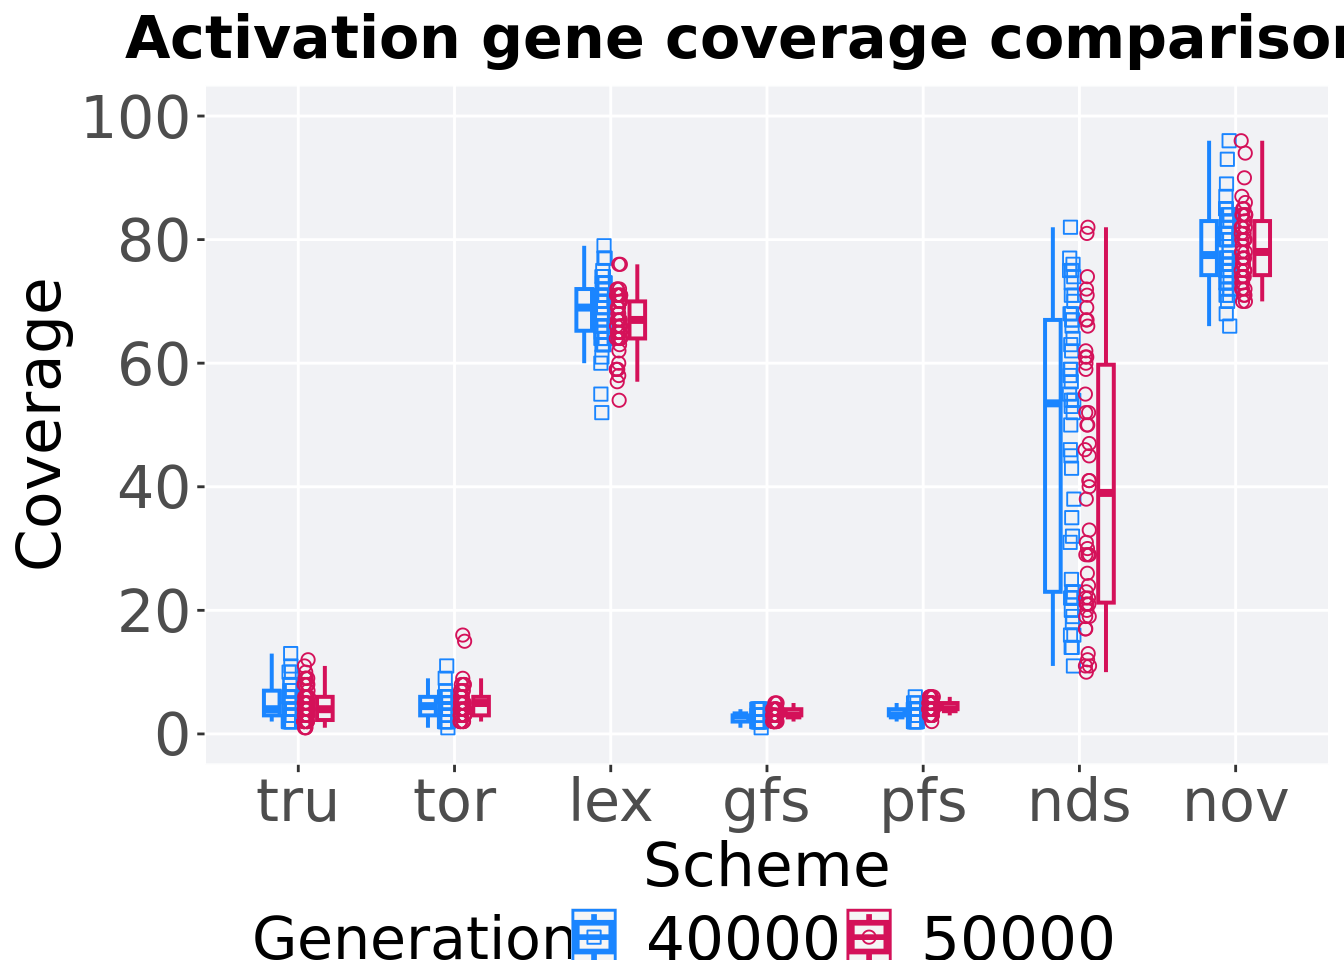
\includegraphics{demo_files/figure-latex/mpe-mvc-act-sli-1.pdf}

\hypertarget{stats-21}{%
\subsubsection{Stats}\label{stats-21}}

Summary statistics for the activation gene coverage at 40,000 and 50,000 generations.

\begin{Shaded}
\begin{Highlighting}[]
\NormalTok{slices =}\StringTok{ }\KeywordTok{filter}\NormalTok{(cc_over_time_mvc, diagnostic }\OperatorTok{==}\StringTok{ 'multipath_exploration'} \OperatorTok{&}\StringTok{ }\NormalTok{(gen }\OperatorTok{==}\StringTok{ }\DecValTok{50000} \OperatorTok{|}\StringTok{ }\NormalTok{gen }\OperatorTok{==}\StringTok{ }\DecValTok{40000}\NormalTok{) }\OperatorTok{&}\StringTok{ }\NormalTok{acron }\OperatorTok{!=}\StringTok{ 'ran'}\NormalTok{)}
\NormalTok{slices}\OperatorTok{$}\NormalTok{Generation <-}\StringTok{ }\KeywordTok{factor}\NormalTok{(slices}\OperatorTok{$}\NormalTok{gen, }\DataTypeTok{levels =} \KeywordTok{c}\NormalTok{(}\DecValTok{50000}\NormalTok{,}\DecValTok{40000}\NormalTok{))}
\NormalTok{slices}\OperatorTok{$}\NormalTok{acron =}\StringTok{ }\KeywordTok{factor}\NormalTok{(slices}\OperatorTok{$}\NormalTok{acron, }\DataTypeTok{levels =} \KeywordTok{c}\NormalTok{(}\StringTok{'nov'}\NormalTok{,}\StringTok{'lex'}\NormalTok{, }\StringTok{'nds'}\NormalTok{,}\StringTok{'tru'}\NormalTok{,}\StringTok{'tor'}\NormalTok{,}\StringTok{'gfs'}\NormalTok{,}\StringTok{'pfs'}\NormalTok{,}\StringTok{'ran'}\NormalTok{))}
\NormalTok{slices }\OperatorTok
\StringTok{  }\KeywordTok{group_by}\NormalTok{(acron, Generation) }\OperatorTok
\StringTok{  }\NormalTok{dplyr}\OperatorTok{::}\KeywordTok{summarise}\NormalTok{(}
    \DataTypeTok{count =} \KeywordTok{n}\NormalTok{(),}
    \DataTypeTok{na_cnt =} \KeywordTok{sum}\NormalTok{(}\KeywordTok{is.na}\NormalTok{(uni_str_pos)),}
    \DataTypeTok{min =} \KeywordTok{min}\NormalTok{(uni_str_pos, }\DataTypeTok{na.rm =} \OtherTok{TRUE}\NormalTok{),}
    \DataTypeTok{median =} \KeywordTok{median}\NormalTok{(uni_str_pos, }\DataTypeTok{na.rm =} \OtherTok{TRUE}\NormalTok{),}
    \DataTypeTok{mean =} \KeywordTok{mean}\NormalTok{(uni_str_pos, }\DataTypeTok{na.rm =} \OtherTok{TRUE}\NormalTok{),}
    \DataTypeTok{max =} \KeywordTok{max}\NormalTok{(uni_str_pos, }\DataTypeTok{na.rm =} \OtherTok{TRUE}\NormalTok{),}
    \DataTypeTok{IQR =} \KeywordTok{IQR}\NormalTok{(uni_str_pos, }\DataTypeTok{na.rm =} \OtherTok{TRUE}\NormalTok{)}
\NormalTok{  )}
\end{Highlighting}
\end{Shaded}

\begin{verbatim}
## `summarise()` has grouped output by 'acron'. You can override using the
## `.groups` argument.
\end{verbatim}

\begin{verbatim}
## # A tibble: 14 x 9
## # Groups:   acron [7]
##    acron Generation count na_cnt   min median  mean   max   IQR
##    <fct> <fct>      <int>  <int> <int>  <dbl> <dbl> <int> <dbl>
##  1 nov   50000         50      0    70   78   79.1     96  8.75
##  2 nov   40000         50      0    66   77.5 78.6     96  8.75
##  3 lex   50000         50      0    54   67   66.6     76  6   
##  4 lex   40000         50      0    52   69   68.3     79  6.75
##  5 nds   50000         50      0    10   39   40.4     82 38.5 
##  6 nds   40000         50      0    11   53.5 47.5     82 44   
##  7 tru   50000         50      0     1    4    4.8     12  3.75
##  8 tru   40000         50      0     2    4    4.78    13  4   
##  9 tor   50000         50      0     2    5    5.1     16  3   
## 10 tor   40000         50      0     1    4.5  4.38    11  3   
## 11 gfs   50000         50      0     2    3    3.14     5  1   
## 12 gfs   40000         50      0     1    3    2.72     4  1   
## 13 pfs   50000         50      0     2    4    4.34     6  1   
## 14 pfs   40000         50      0     2    3    3.28     6  1
\end{verbatim}

Truncation selection comparisons.

\begin{Shaded}
\begin{Highlighting}[]
\KeywordTok{wilcox.test}\NormalTok{(}\DataTypeTok{x =} \KeywordTok{filter}\NormalTok{(slices, acron }\OperatorTok{==}\StringTok{ 'tru'} \OperatorTok{&}\StringTok{ }\NormalTok{Generation }\OperatorTok{==}\StringTok{ }\DecValTok{50000}\NormalTok{)}\OperatorTok{$}\NormalTok{uni_str_pos,}
            \DataTypeTok{y =} \KeywordTok{filter}\NormalTok{(slices, acron }\OperatorTok{==}\StringTok{ 'tru'} \OperatorTok{&}\StringTok{ }\NormalTok{Generation }\OperatorTok{==}\StringTok{ }\DecValTok{40000}\NormalTok{)}\OperatorTok{$}\NormalTok{uni_str_pos,}
            \DataTypeTok{alternative =} \StringTok{'t'}\NormalTok{)}
\end{Highlighting}
\end{Shaded}

\begin{verbatim}
## 
##  Wilcoxon rank sum test with continuity correction
## 
## data:  filter(slices, acron == "tru" & Generation == 50000)$uni_str_pos and filter(slices, acron == "tru" & Generation == 40000)$uni_str_pos
## W = 1254.5, p-value = 0.9778
## alternative hypothesis: true location shift is not equal to 0
\end{verbatim}

Tournament selection comparisons.

\begin{Shaded}
\begin{Highlighting}[]
\KeywordTok{wilcox.test}\NormalTok{(}\DataTypeTok{x =} \KeywordTok{filter}\NormalTok{(slices, acron }\OperatorTok{==}\StringTok{ 'tor'} \OperatorTok{&}\StringTok{ }\NormalTok{Generation }\OperatorTok{==}\StringTok{ }\DecValTok{50000}\NormalTok{)}\OperatorTok{$}\NormalTok{uni_str_pos,}
            \DataTypeTok{y =} \KeywordTok{filter}\NormalTok{(slices, acron }\OperatorTok{==}\StringTok{ 'tor'} \OperatorTok{&}\StringTok{ }\NormalTok{Generation }\OperatorTok{==}\StringTok{ }\DecValTok{40000}\NormalTok{)}\OperatorTok{$}\NormalTok{uni_str_pos,}
            \DataTypeTok{alternative =} \StringTok{'t'}\NormalTok{)}
\end{Highlighting}
\end{Shaded}

\begin{verbatim}
## 
##  Wilcoxon rank sum test with continuity correction
## 
## data:  filter(slices, acron == "tor" & Generation == 50000)$uni_str_pos and filter(slices, acron == "tor" & Generation == 40000)$uni_str_pos
## W = 1396, p-value = 0.3094
## alternative hypothesis: true location shift is not equal to 0
\end{verbatim}

Lexicase selection comparisons.

\begin{Shaded}
\begin{Highlighting}[]
\KeywordTok{wilcox.test}\NormalTok{(}\DataTypeTok{x =} \KeywordTok{filter}\NormalTok{(slices, acron }\OperatorTok{==}\StringTok{ 'lex'} \OperatorTok{&}\StringTok{ }\NormalTok{Generation }\OperatorTok{==}\StringTok{ }\DecValTok{50000}\NormalTok{)}\OperatorTok{$}\NormalTok{uni_str_pos,}
            \DataTypeTok{y =} \KeywordTok{filter}\NormalTok{(slices, acron }\OperatorTok{==}\StringTok{ 'lex'} \OperatorTok{&}\StringTok{ }\NormalTok{Generation }\OperatorTok{==}\StringTok{ }\DecValTok{40000}\NormalTok{)}\OperatorTok{$}\NormalTok{uni_str_pos,}
            \DataTypeTok{alternative =} \StringTok{'t'}\NormalTok{)}
\end{Highlighting}
\end{Shaded}

\begin{verbatim}
## 
##  Wilcoxon rank sum test with continuity correction
## 
## data:  filter(slices, acron == "lex" & Generation == 50000)$uni_str_pos and filter(slices, acron == "lex" & Generation == 40000)$uni_str_pos
## W = 992.5, p-value = 0.07568
## alternative hypothesis: true location shift is not equal to 0
\end{verbatim}

Genotypic fitness sharing comparisons.

\begin{Shaded}
\begin{Highlighting}[]
\KeywordTok{wilcox.test}\NormalTok{(}\DataTypeTok{x =} \KeywordTok{filter}\NormalTok{(slices, acron }\OperatorTok{==}\StringTok{ 'gfs'} \OperatorTok{&}\StringTok{ }\NormalTok{Generation }\OperatorTok{==}\StringTok{ }\DecValTok{50000}\NormalTok{)}\OperatorTok{$}\NormalTok{uni_str_pos,}
            \DataTypeTok{y =} \KeywordTok{filter}\NormalTok{(slices, acron }\OperatorTok{==}\StringTok{ 'gfs'} \OperatorTok{&}\StringTok{ }\NormalTok{Generation }\OperatorTok{==}\StringTok{ }\DecValTok{40000}\NormalTok{)}\OperatorTok{$}\NormalTok{uni_str_pos,}
            \DataTypeTok{alternative =} \StringTok{'t'}\NormalTok{)}
\end{Highlighting}
\end{Shaded}

\begin{verbatim}
## 
##  Wilcoxon rank sum test with continuity correction
## 
## data:  filter(slices, acron == "gfs" & Generation == 50000)$uni_str_pos and filter(slices, acron == "gfs" & Generation == 40000)$uni_str_pos
## W = 1573, p-value = 0.01769
## alternative hypothesis: true location shift is not equal to 0
\end{verbatim}

Phenotypic fitness sharing comparisons.

\begin{Shaded}
\begin{Highlighting}[]
\KeywordTok{wilcox.test}\NormalTok{(}\DataTypeTok{x =} \KeywordTok{filter}\NormalTok{(slices, acron }\OperatorTok{==}\StringTok{ 'pfs'} \OperatorTok{&}\StringTok{ }\NormalTok{Generation }\OperatorTok{==}\StringTok{ }\DecValTok{50000}\NormalTok{)}\OperatorTok{$}\NormalTok{uni_str_pos,}
            \DataTypeTok{y =} \KeywordTok{filter}\NormalTok{(slices, acron }\OperatorTok{==}\StringTok{ 'pfs'} \OperatorTok{&}\StringTok{ }\NormalTok{Generation }\OperatorTok{==}\StringTok{ }\DecValTok{40000}\NormalTok{)}\OperatorTok{$}\NormalTok{uni_str_pos,}
            \DataTypeTok{alternative =} \StringTok{'t'}\NormalTok{)}
\end{Highlighting}
\end{Shaded}

\begin{verbatim}
## 
##  Wilcoxon rank sum test with continuity correction
## 
## data:  filter(slices, acron == "pfs" & Generation == 50000)$uni_str_pos and filter(slices, acron == "pfs" & Generation == 40000)$uni_str_pos
## W = 1914.5, p-value = 2.023e-06
## alternative hypothesis: true location shift is not equal to 0
\end{verbatim}

Nondominated sorting comparisons.

\begin{Shaded}
\begin{Highlighting}[]
\KeywordTok{wilcox.test}\NormalTok{(}\DataTypeTok{x =} \KeywordTok{filter}\NormalTok{(slices, acron }\OperatorTok{==}\StringTok{ 'nds'} \OperatorTok{&}\StringTok{ }\NormalTok{Generation }\OperatorTok{==}\StringTok{ }\DecValTok{50000}\NormalTok{)}\OperatorTok{$}\NormalTok{uni_str_pos,}
            \DataTypeTok{y =} \KeywordTok{filter}\NormalTok{(slices, acron }\OperatorTok{==}\StringTok{ 'nds'} \OperatorTok{&}\StringTok{ }\NormalTok{Generation }\OperatorTok{==}\StringTok{ }\DecValTok{40000}\NormalTok{)}\OperatorTok{$}\NormalTok{uni_str_pos,}
            \DataTypeTok{alternative =} \StringTok{'t'}\NormalTok{)}
\end{Highlighting}
\end{Shaded}

\begin{verbatim}
## 
##  Wilcoxon rank sum test with continuity correction
## 
## data:  filter(slices, acron == "nds" & Generation == 50000)$uni_str_pos and filter(slices, acron == "nds" & Generation == 40000)$uni_str_pos
## W = 1008, p-value = 0.09584
## alternative hypothesis: true location shift is not equal to 0
\end{verbatim}

Novelty search comparisons.

\begin{Shaded}
\begin{Highlighting}[]
\KeywordTok{wilcox.test}\NormalTok{(}\DataTypeTok{x =} \KeywordTok{filter}\NormalTok{(slices, acron }\OperatorTok{==}\StringTok{ 'nov'} \OperatorTok{&}\StringTok{ }\NormalTok{Generation }\OperatorTok{==}\StringTok{ }\DecValTok{50000}\NormalTok{)}\OperatorTok{$}\NormalTok{uni_str_pos,}
            \DataTypeTok{y =} \KeywordTok{filter}\NormalTok{(slices, acron }\OperatorTok{==}\StringTok{ 'nov'} \OperatorTok{&}\StringTok{ }\NormalTok{Generation }\OperatorTok{==}\StringTok{ }\DecValTok{40000}\NormalTok{)}\OperatorTok{$}\NormalTok{uni_str_pos,}
            \DataTypeTok{alternative =} \StringTok{'t'}\NormalTok{)}
\end{Highlighting}
\end{Shaded}

\begin{verbatim}
## 
##  Wilcoxon rank sum test with continuity correction
## 
## data:  filter(slices, acron == "nov" & Generation == 50000)$uni_str_pos and filter(slices, acron == "nov" & Generation == 40000)$uni_str_pos
## W = 1295.5, p-value = 0.756
## alternative hypothesis: true location shift is not equal to 0
\end{verbatim}

\hypertarget{truncation-selection}{%
\chapter{Truncation selection}\label{truncation-selection}}

We present the results from our parameter sweeep on truncation selection.
50 replicates are conducted for each truncation size \texttt{T} parameter value explored.

\begin{Shaded}
\begin{Highlighting}[]
\KeywordTok{library}\NormalTok{(ggplot2)}
\KeywordTok{library}\NormalTok{(cowplot)}
\KeywordTok{library}\NormalTok{(dplyr)}
\KeywordTok{library}\NormalTok{(PupillometryR)}
\end{Highlighting}
\end{Shaded}

\hypertarget{exploitation-rate-results-1}{%
\section{Exploitation rate results}\label{exploitation-rate-results-1}}

Here we present the results for \textbf{best performances} found by each truncation selection value replicate on the exploitation rate diagnostic.

\hypertarget{performance-over-time-5}{%
\subsection{Performance over time}\label{performance-over-time-5}}

Performance over time.

\begin{Shaded}
\begin{Highlighting}[]
\NormalTok{lines =}\StringTok{ }\KeywordTok{filter}\NormalTok{(tru_ot, diagnostic }\OperatorTok{==}\StringTok{ 'exploitation_rate'}\NormalTok{) }\OperatorTok
\StringTok{        }\KeywordTok{group_by}\NormalTok{(T, gen) }\OperatorTok
\StringTok{          }\NormalTok{dplyr}\OperatorTok{::}\KeywordTok{summarise}\NormalTok{(}
            \DataTypeTok{min =} \KeywordTok{min}\NormalTok{(pop_fit_max),}
            \DataTypeTok{mean =} \KeywordTok{mean}\NormalTok{(pop_fit_max),}
            \DataTypeTok{max =} \KeywordTok{max}\NormalTok{(pop_fit_max)}
\NormalTok{          )}
\end{Highlighting}
\end{Shaded}

\begin{verbatim}
## `summarise()` has grouped output by 'T'. You can override using the `.groups`
## argument.
\end{verbatim}

\begin{Shaded}
\begin{Highlighting}[]
\KeywordTok{ggplot}\NormalTok{(lines, }\KeywordTok{aes}\NormalTok{(}\DataTypeTok{x=}\NormalTok{gen, }\DataTypeTok{y=}\NormalTok{mean }\OperatorTok{/}\StringTok{ }\NormalTok{DIMENSIONALITY, }\DataTypeTok{group =}\NormalTok{ T, }\DataTypeTok{fill =}\NormalTok{ T, }\DataTypeTok{color =}\NormalTok{ T, }\DataTypeTok{shape =}\NormalTok{ T)) }\OperatorTok{+}
\StringTok{  }\KeywordTok{geom_ribbon}\NormalTok{(}\KeywordTok{aes}\NormalTok{(}\DataTypeTok{ymin =}\NormalTok{ min }\OperatorTok{/}\StringTok{ }\NormalTok{DIMENSIONALITY, }\DataTypeTok{ymax =}\NormalTok{ max }\OperatorTok{/}\StringTok{ }\NormalTok{DIMENSIONALITY), }\DataTypeTok{alpha =} \FloatTok{0.1}\NormalTok{) }\OperatorTok{+}
\StringTok{  }\KeywordTok{geom_line}\NormalTok{(}\DataTypeTok{size =} \FloatTok{0.5}\NormalTok{) }\OperatorTok{+}
\StringTok{  }\KeywordTok{geom_point}\NormalTok{(}\DataTypeTok{data =} \KeywordTok{filter}\NormalTok{(lines, gen }\OperatorTok\StringTok{ }\DecValTok{2000} \OperatorTok{==}\StringTok{ }\DecValTok{0} \OperatorTok{&}\StringTok{ }\NormalTok{gen }\OperatorTok{!=}\StringTok{ }\DecValTok{0}\NormalTok{), }\DataTypeTok{size =} \FloatTok{1.5}\NormalTok{, }\DataTypeTok{stroke =} \FloatTok{2.0}\NormalTok{, }\DataTypeTok{alpha =} \FloatTok{1.0}\NormalTok{) }\OperatorTok{+}
\StringTok{  }\KeywordTok{scale_y_continuous}\NormalTok{(}
    \DataTypeTok{name=}\StringTok{"Average trait score"}
\NormalTok{  ) }\OperatorTok{+}
\StringTok{  }\KeywordTok{scale_x_continuous}\NormalTok{(}
    \DataTypeTok{name=}\StringTok{"Generations"}\NormalTok{,}
    \DataTypeTok{limits=}\KeywordTok{c}\NormalTok{(}\DecValTok{0}\NormalTok{, }\DecValTok{50000}\NormalTok{),}
    \DataTypeTok{breaks=}\KeywordTok{c}\NormalTok{(}\DecValTok{0}\NormalTok{, }\DecValTok{10000}\NormalTok{, }\DecValTok{20000}\NormalTok{, }\DecValTok{30000}\NormalTok{, }\DecValTok{40000}\NormalTok{, }\DecValTok{50000}\NormalTok{),}
    \DataTypeTok{labels=}\KeywordTok{c}\NormalTok{(}\StringTok{"0e+4"}\NormalTok{, }\StringTok{"1e+4"}\NormalTok{, }\StringTok{"2e+4"}\NormalTok{, }\StringTok{"3e+4"}\NormalTok{, }\StringTok{"4e+4"}\NormalTok{, }\StringTok{"5e+4"}\NormalTok{)}

\NormalTok{  ) }\OperatorTok{+}
\StringTok{  }\KeywordTok{scale_shape_manual}\NormalTok{(}\DataTypeTok{values=}\NormalTok{SHAPE)}\OperatorTok{+}
\StringTok{  }\KeywordTok{scale_colour_manual}\NormalTok{(}\DataTypeTok{values =}\NormalTok{ cb_palette) }\OperatorTok{+}
\StringTok{  }\KeywordTok{scale_fill_manual}\NormalTok{(}\DataTypeTok{values =}\NormalTok{ cb_palette) }\OperatorTok{+}
\StringTok{  }\KeywordTok{ggtitle}\NormalTok{(}\StringTok{"Best performance over time"}\NormalTok{) }\OperatorTok{+}
\StringTok{  }\NormalTok{p_theme}
\end{Highlighting}
\end{Shaded}

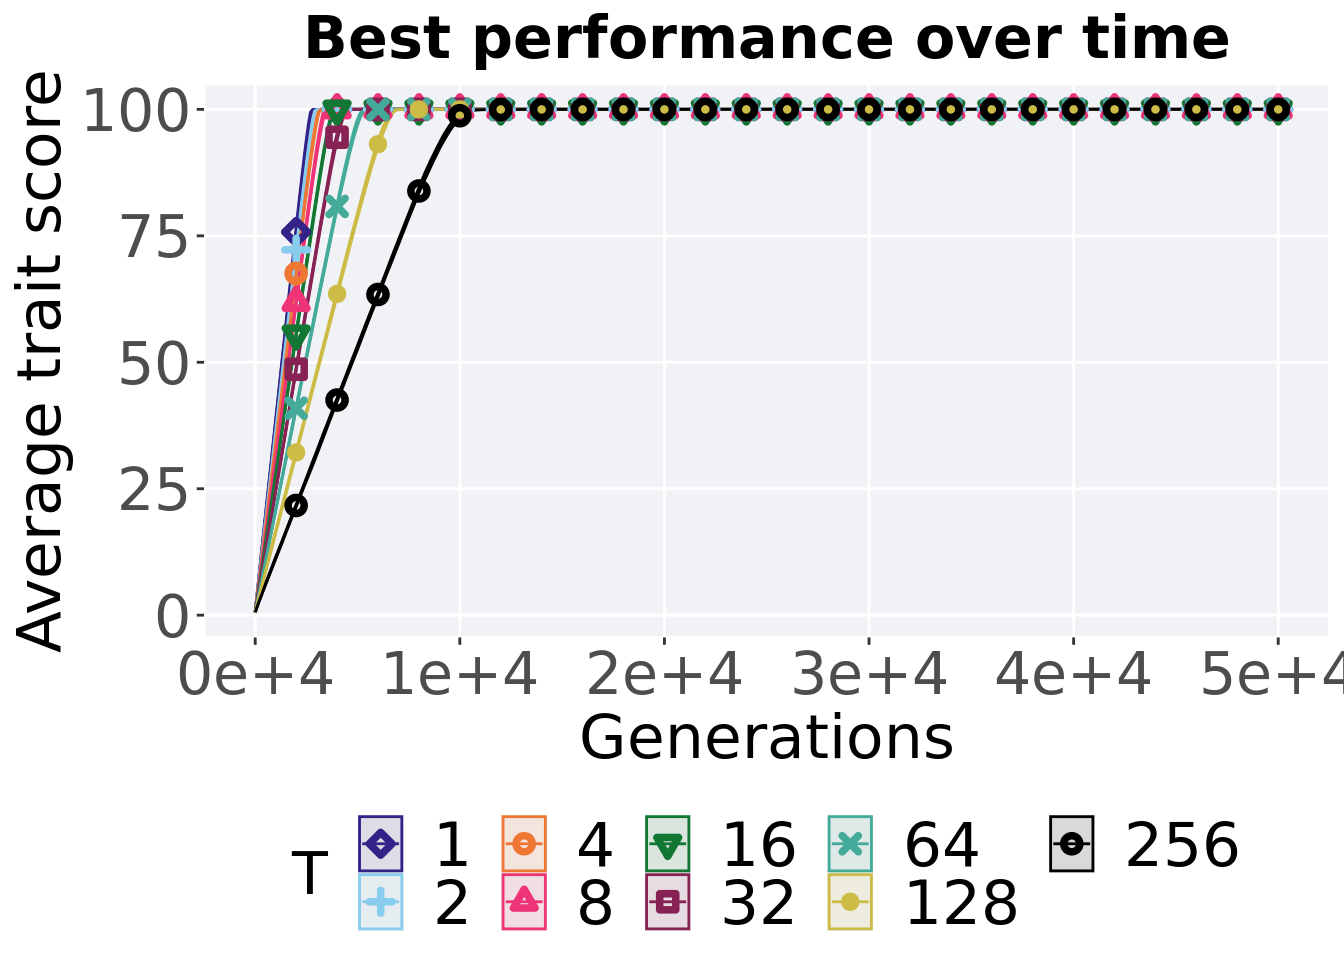
\includegraphics{demo_files/figure-latex/tru-exp-per-1.pdf}

\hypertarget{generation-satisfactory-solution-found-2}{%
\subsection{Generation satisfactory solution found}\label{generation-satisfactory-solution-found-2}}

The first Generations a satisfactory solution is found throughout the 50,000 generations.

\begin{Shaded}
\begin{Highlighting}[]
\KeywordTok{filter}\NormalTok{(tru_ssf, Diagnostic }\OperatorTok{==}\StringTok{ 'EXPLOITATION_RATE'}\NormalTok{) }\OperatorTok
\KeywordTok{ggplot}\NormalTok{(., }\KeywordTok{aes}\NormalTok{(}\DataTypeTok{x =}\NormalTok{ T, }\DataTypeTok{y =}\NormalTok{ Generations, }\DataTypeTok{color =}\NormalTok{ T, }\DataTypeTok{fill =}\NormalTok{ T, }\DataTypeTok{shape =}\NormalTok{ T)) }\OperatorTok{+}
\StringTok{  }\KeywordTok{geom_flat_violin}\NormalTok{(}\DataTypeTok{position =} \KeywordTok{position_nudge}\NormalTok{(}\DataTypeTok{x =} \FloatTok{.2}\NormalTok{, }\DataTypeTok{y =} \DecValTok{0}\NormalTok{), }\DataTypeTok{scale =} \StringTok{'width'}\NormalTok{, }\DataTypeTok{alpha =} \FloatTok{0.2}\NormalTok{) }\OperatorTok{+}
\StringTok{  }\KeywordTok{geom_point}\NormalTok{(}\DataTypeTok{position =} \KeywordTok{position_jitter}\NormalTok{(}\DataTypeTok{width =} \FloatTok{.1}\NormalTok{), }\DataTypeTok{size =} \FloatTok{1.5}\NormalTok{, }\DataTypeTok{alpha =} \FloatTok{1.0}\NormalTok{) }\OperatorTok{+}
\StringTok{  }\KeywordTok{geom_boxplot}\NormalTok{(}\DataTypeTok{color =} \StringTok{'black'}\NormalTok{, }\DataTypeTok{width =} \FloatTok{.2}\NormalTok{, }\DataTypeTok{outlier.shape =} \OtherTok{NA}\NormalTok{, }\DataTypeTok{alpha =} \FloatTok{0.0}\NormalTok{) }\OperatorTok{+}
\StringTok{  }\KeywordTok{scale_shape_manual}\NormalTok{(}\DataTypeTok{values=}\NormalTok{SHAPE)}\OperatorTok{+}
\StringTok{  }\KeywordTok{scale_y_continuous}\NormalTok{(}
    \DataTypeTok{name=}\StringTok{"Generation"}\NormalTok{,}
    \DataTypeTok{limits=}\KeywordTok{c}\NormalTok{(}\DecValTok{0}\NormalTok{, }\DecValTok{12000}\NormalTok{),}
    \DataTypeTok{breaks=}\KeywordTok{c}\NormalTok{(}\DecValTok{0}\NormalTok{, }\DecValTok{2000}\NormalTok{, }\DecValTok{4000}\NormalTok{, }\DecValTok{6000}\NormalTok{, }\DecValTok{8000}\NormalTok{, }\DecValTok{10000}\NormalTok{, }\DecValTok{12000}\NormalTok{),}
    \DataTypeTok{labels=}\KeywordTok{c}\NormalTok{(}\StringTok{"0e+4"}\NormalTok{, }\StringTok{"2e+4"}\NormalTok{, }\StringTok{"4e+4"}\NormalTok{, }\StringTok{"6e+4"}\NormalTok{, }\StringTok{"8e+4"}\NormalTok{, }\StringTok{"10e+4"}\NormalTok{, }\StringTok{"12e+4"}\NormalTok{)}
\NormalTok{  ) }\OperatorTok{+}
\StringTok{  }\KeywordTok{scale_x_discrete}\NormalTok{(}
    \DataTypeTok{name=}\StringTok{"T"}
\NormalTok{  ) }\OperatorTok{+}
\StringTok{  }\KeywordTok{ggtitle}\NormalTok{(}\StringTok{"Generation satisfactory solution found"}\NormalTok{) }\OperatorTok{+}
\StringTok{  }\KeywordTok{scale_colour_manual}\NormalTok{(}\DataTypeTok{values =}\NormalTok{ cb_palette) }\OperatorTok{+}
\StringTok{  }\KeywordTok{scale_fill_manual}\NormalTok{(}\DataTypeTok{values =}\NormalTok{ cb_palette) }\OperatorTok{+}
\StringTok{  }\NormalTok{p_theme}
\end{Highlighting}
\end{Shaded}

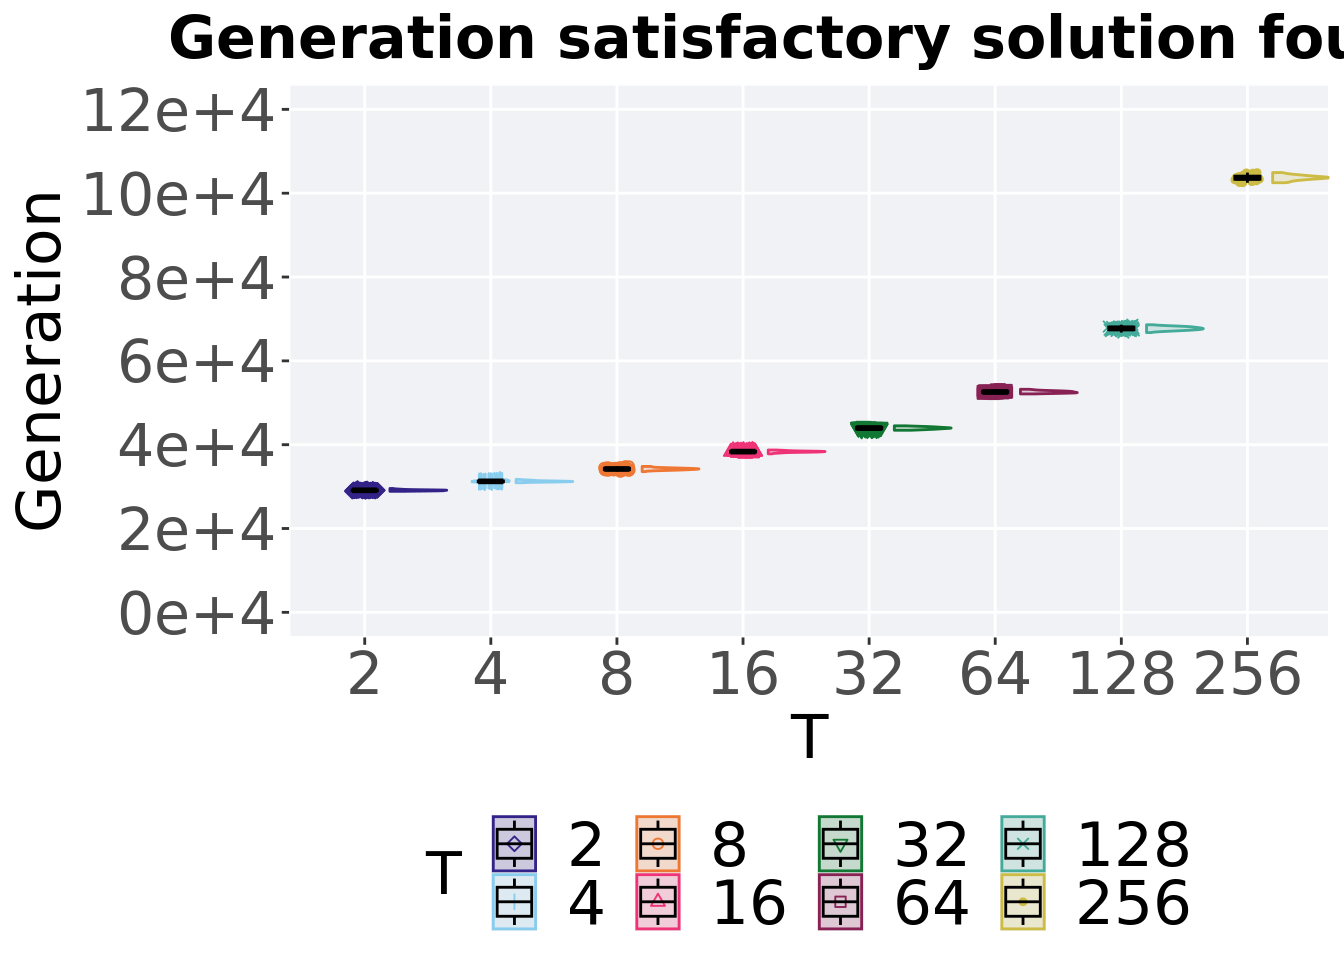
\includegraphics{demo_files/figure-latex/tru-exp-ssf-1.pdf}

\hypertarget{stats-22}{%
\subsubsection{Stats}\label{stats-22}}

Summary statistics for the best performance found throughout 50,000 generations.

\begin{Shaded}
\begin{Highlighting}[]
\NormalTok{ssf =}\StringTok{ }\KeywordTok{filter}\NormalTok{(tru_ssf, Diagnostic }\OperatorTok{==}\StringTok{ 'EXPLOITATION_RATE'}\NormalTok{)}
\KeywordTok{group_by}\NormalTok{(ssf, T) }\OperatorTok
\StringTok{  }\NormalTok{dplyr}\OperatorTok{::}\KeywordTok{summarise}\NormalTok{(}
    \DataTypeTok{count =} \KeywordTok{n}\NormalTok{(),}
    \DataTypeTok{na_cnt =} \KeywordTok{sum}\NormalTok{(}\KeywordTok{is.na}\NormalTok{(Generations)),}
    \DataTypeTok{min =} \KeywordTok{min}\NormalTok{(Generations, }\DataTypeTok{na.rm =} \OtherTok{TRUE}\NormalTok{),}
    \DataTypeTok{median =} \KeywordTok{median}\NormalTok{(Generations, }\DataTypeTok{na.rm =} \OtherTok{TRUE}\NormalTok{),}
    \DataTypeTok{mean =} \KeywordTok{mean}\NormalTok{(Generations, }\DataTypeTok{na.rm =} \OtherTok{TRUE}\NormalTok{),}
    \DataTypeTok{max =} \KeywordTok{max}\NormalTok{(Generations, }\DataTypeTok{na.rm =} \OtherTok{TRUE}\NormalTok{),}
    \DataTypeTok{IQR =} \KeywordTok{IQR}\NormalTok{(Generations, }\DataTypeTok{na.rm =} \OtherTok{TRUE}\NormalTok{)}
\NormalTok{  )}
\end{Highlighting}
\end{Shaded}

\begin{verbatim}
## # A tibble: 8 x 8
##   T     count na_cnt   min median   mean   max   IQR
##   <fct> <int>  <int> <int>  <dbl>  <dbl> <int> <dbl>
## 1 2        50      0  2887  2912   2912.  2955  18.2
## 2 4        50      0  3091  3125   3126.  3171  19  
## 3 8        50      0  3357  3420   3421.  3481  34.2
## 4 16       50      0  3781  3834.  3833.  3873  20.8
## 5 32       50      0  4344  4396.  4396.  4450  41.2
## 6 64       50      0  5211  5256.  5259.  5322  38  
## 7 128      50      0  6675  6773   6772.  6861  62  
## 8 256      50      0 10250 10368. 10369. 10492  73.2
\end{verbatim}

Kruskal--Wallis test provides evidence of significant differences among the Generations a satisfactory solution is first found.

\begin{Shaded}
\begin{Highlighting}[]
\KeywordTok{kruskal.test}\NormalTok{(Generations }\OperatorTok{~}\StringTok{ }\NormalTok{T,}\DataTypeTok{data =}\NormalTok{ ssf)}
\end{Highlighting}
\end{Shaded}

\begin{verbatim}
## 
##  Kruskal-Wallis rank sum test
## 
## data:  Generations by T
## Kruskal-Wallis chi-squared = 392.77, df = 7, p-value < 2.2e-16
\end{verbatim}

Results for post-hoc Wilcoxon rank-sum test with a Bonferroni correction on the Generations a satisfactory solution is first found. .

\begin{Shaded}
\begin{Highlighting}[]
\KeywordTok{pairwise.wilcox.test}\NormalTok{(}\DataTypeTok{x =}\NormalTok{ ssf}\OperatorTok{$}\NormalTok{Generations, }\DataTypeTok{g =}\NormalTok{ ssf}\OperatorTok{$}\NormalTok{T , }\DataTypeTok{p.adjust.method =} \StringTok{"bonferroni"}\NormalTok{,}
                     \DataTypeTok{paired =} \OtherTok{FALSE}\NormalTok{, }\DataTypeTok{conf.int =} \OtherTok{FALSE}\NormalTok{, }\DataTypeTok{alternative =} \StringTok{'g'}\NormalTok{)}
\end{Highlighting}
\end{Shaded}

\begin{verbatim}
## 
##  Pairwise comparisons using Wilcoxon rank sum test with continuity correction 
## 
## data:  ssf$Generations and ssf$T 
## 
##     2      4      8      16     32     64     128   
## 4   <2e-16 -      -      -      -      -      -     
## 8   <2e-16 <2e-16 -      -      -      -      -     
## 16  <2e-16 <2e-16 <2e-16 -      -      -      -     
## 32  <2e-16 <2e-16 <2e-16 <2e-16 -      -      -     
## 64  <2e-16 <2e-16 <2e-16 <2e-16 <2e-16 -      -     
## 128 <2e-16 <2e-16 <2e-16 <2e-16 <2e-16 <2e-16 -     
## 256 <2e-16 <2e-16 <2e-16 <2e-16 <2e-16 <2e-16 <2e-16
## 
## P value adjustment method: bonferroni
\end{verbatim}

\hypertarget{multi-valley-crossing}{%
\subsection{Multi-valley crossing}\label{multi-valley-crossing}}

\hypertarget{performance-over-time-6}{%
\subsubsection{Performance over time}\label{performance-over-time-6}}

\begin{Shaded}
\begin{Highlighting}[]
\CommentTok{# data for lines and shading on plots}
\NormalTok{lines =}\StringTok{ }\KeywordTok{filter}\NormalTok{(tru_ot_mvc, diagnostic }\OperatorTok{==}\StringTok{ 'exploitation_rate'}\NormalTok{) }\OperatorTok
\StringTok{  }\KeywordTok{group_by}\NormalTok{(T, gen) }\OperatorTok
\StringTok{  }\NormalTok{dplyr}\OperatorTok{::}\KeywordTok{summarise}\NormalTok{(}
    \DataTypeTok{min =} \KeywordTok{min}\NormalTok{(pop_fit_max) }\OperatorTok{/}\StringTok{ }\NormalTok{DIMENSIONALITY,}
    \DataTypeTok{mean =} \KeywordTok{mean}\NormalTok{(pop_fit_max) }\OperatorTok{/}\StringTok{ }\NormalTok{DIMENSIONALITY,}
    \DataTypeTok{max =} \KeywordTok{max}\NormalTok{(pop_fit_max) }\OperatorTok{/}\StringTok{ }\NormalTok{DIMENSIONALITY}
\NormalTok{  )}
\end{Highlighting}
\end{Shaded}

\begin{verbatim}
## `summarise()` has grouped output by 'T'. You can override using the `.groups`
## argument.
\end{verbatim}

\begin{Shaded}
\begin{Highlighting}[]
\KeywordTok{ggplot}\NormalTok{(lines, }\KeywordTok{aes}\NormalTok{(}\DataTypeTok{x=}\NormalTok{gen, }\DataTypeTok{y=}\NormalTok{mean, }\DataTypeTok{group =}\NormalTok{ T, }\DataTypeTok{fill =}\NormalTok{T, }\DataTypeTok{color =}\NormalTok{ T, }\DataTypeTok{shape =}\NormalTok{ T)) }\OperatorTok{+}
\StringTok{  }\KeywordTok{geom_ribbon}\NormalTok{(}\KeywordTok{aes}\NormalTok{(}\DataTypeTok{ymin =}\NormalTok{ min, }\DataTypeTok{ymax =}\NormalTok{ max), }\DataTypeTok{alpha =} \FloatTok{0.1}\NormalTok{) }\OperatorTok{+}
\StringTok{  }\KeywordTok{geom_line}\NormalTok{(}\DataTypeTok{size =} \FloatTok{0.5}\NormalTok{) }\OperatorTok{+}
\StringTok{  }\KeywordTok{geom_point}\NormalTok{(}\DataTypeTok{data =} \KeywordTok{filter}\NormalTok{(lines, gen }\OperatorTok\StringTok{ }\DecValTok{2000} \OperatorTok{==}\StringTok{ }\DecValTok{0} \OperatorTok{&}\StringTok{ }\NormalTok{gen }\OperatorTok{!=}\StringTok{ }\DecValTok{0}\NormalTok{), }\DataTypeTok{size =} \FloatTok{1.5}\NormalTok{, }\DataTypeTok{stroke =} \FloatTok{2.0}\NormalTok{, }\DataTypeTok{alpha =} \FloatTok{1.0}\NormalTok{) }\OperatorTok{+}
\StringTok{  }\KeywordTok{scale_y_continuous}\NormalTok{(}
    \DataTypeTok{name=}\StringTok{"Average trait score"}
\NormalTok{  ) }\OperatorTok{+}
\StringTok{  }\KeywordTok{scale_x_continuous}\NormalTok{(}
    \DataTypeTok{name=}\StringTok{"Generations"}\NormalTok{,}
    \DataTypeTok{limits=}\KeywordTok{c}\NormalTok{(}\DecValTok{0}\NormalTok{, }\DecValTok{50000}\NormalTok{),}
    \DataTypeTok{breaks=}\KeywordTok{c}\NormalTok{(}\DecValTok{0}\NormalTok{, }\DecValTok{10000}\NormalTok{, }\DecValTok{20000}\NormalTok{, }\DecValTok{30000}\NormalTok{, }\DecValTok{40000}\NormalTok{, }\DecValTok{50000}\NormalTok{),}
    \DataTypeTok{labels=}\KeywordTok{c}\NormalTok{(}\StringTok{"0e+4"}\NormalTok{, }\StringTok{"1e+4"}\NormalTok{, }\StringTok{"2e+4"}\NormalTok{, }\StringTok{"3e+4"}\NormalTok{, }\StringTok{"4e+4"}\NormalTok{, }\StringTok{"5e+4"}\NormalTok{)}

\NormalTok{  ) }\OperatorTok{+}
\StringTok{  }\KeywordTok{scale_shape_manual}\NormalTok{(}\DataTypeTok{values=}\NormalTok{SHAPE)}\OperatorTok{+}
\StringTok{  }\KeywordTok{scale_colour_manual}\NormalTok{(}\DataTypeTok{values =}\NormalTok{ cb_palette) }\OperatorTok{+}
\StringTok{  }\KeywordTok{scale_fill_manual}\NormalTok{(}\DataTypeTok{values =}\NormalTok{ cb_palette) }\OperatorTok{+}
\StringTok{  }\KeywordTok{ggtitle}\NormalTok{(}\StringTok{'Performance over time'}\NormalTok{)}\OperatorTok{+}
\StringTok{  }\NormalTok{p_theme }\OperatorTok{+}
\StringTok{  }\KeywordTok{guides}\NormalTok{(}
    \DataTypeTok{shape=}\KeywordTok{guide_legend}\NormalTok{(}\DataTypeTok{nrow=}\DecValTok{2}\NormalTok{, }\DataTypeTok{title.position =} \StringTok{"left"}\NormalTok{),}
    \DataTypeTok{color=}\KeywordTok{guide_legend}\NormalTok{(}\DataTypeTok{nrow=}\DecValTok{2}\NormalTok{, }\DataTypeTok{title.position =} \StringTok{"left"}\NormalTok{),}
    \DataTypeTok{fill=}\KeywordTok{guide_legend}\NormalTok{(}\DataTypeTok{nrow=}\DecValTok{2}\NormalTok{, }\DataTypeTok{title.position =} \StringTok{"left"}\NormalTok{)}
\NormalTok{  )}
\end{Highlighting}
\end{Shaded}

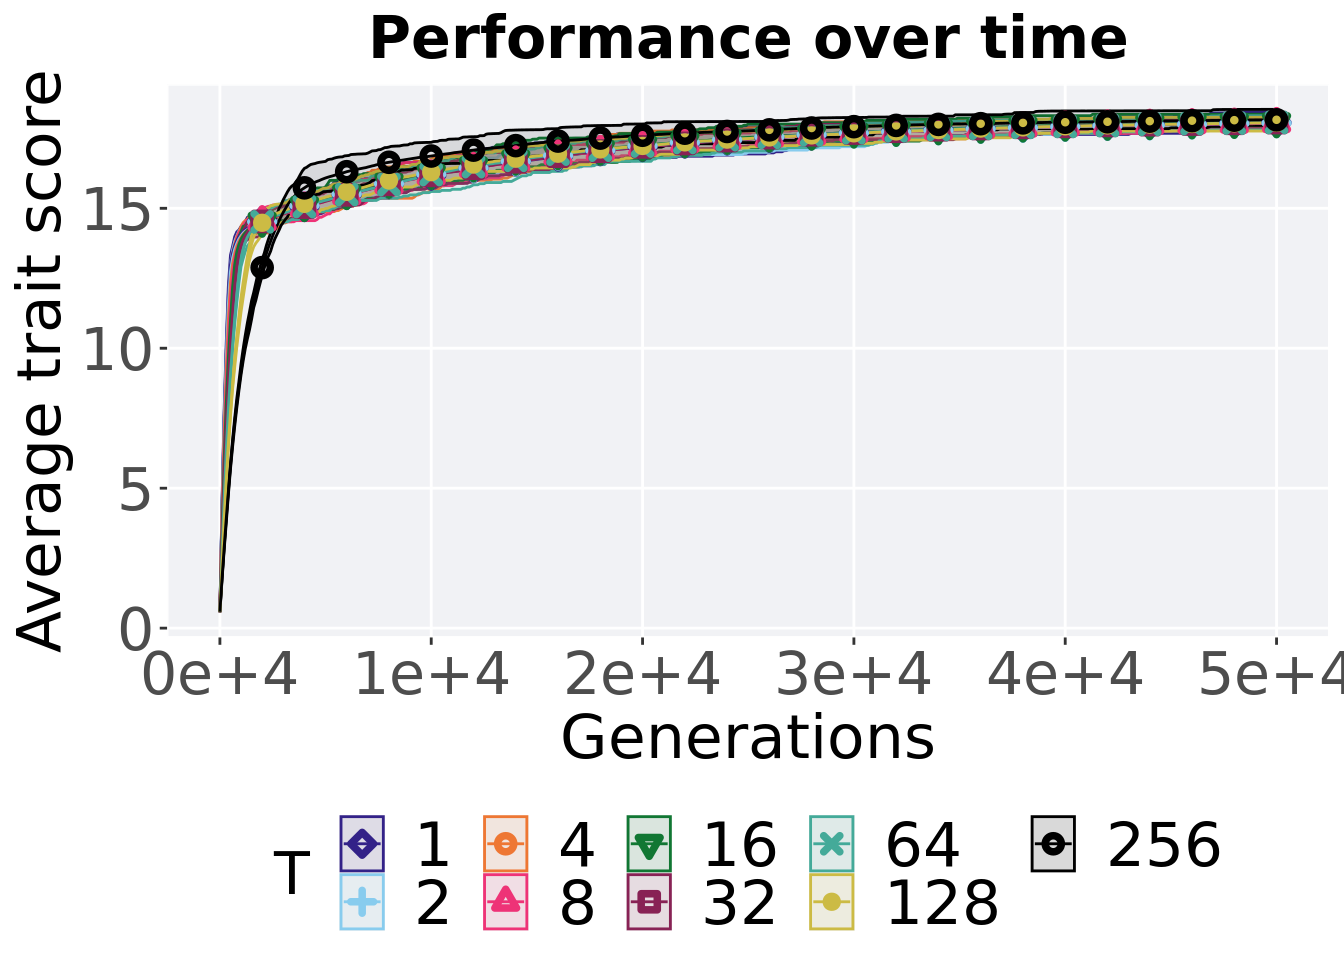
\includegraphics{demo_files/figure-latex/tru-exp-mvc-per-1.pdf}

\hypertarget{performance-comparison-3}{%
\subsubsection{Performance comparison}\label{performance-comparison-3}}

Best performances in the population at 40,000 and 50,000 generations.

\begin{Shaded}
\begin{Highlighting}[]
\CommentTok{# 80% and final generation comparison}
\NormalTok{end =}\StringTok{ }\KeywordTok{filter}\NormalTok{(tru_ot_mvc, diagnostic }\OperatorTok{==}\StringTok{ 'exploitation_rate'} \OperatorTok{&}\StringTok{ }\NormalTok{gen }\OperatorTok{==}\StringTok{ }\DecValTok{50000} \OperatorTok{&}\StringTok{ }\NormalTok{T }\OperatorTok{!=}\StringTok{ 'ran'}\NormalTok{)}
\NormalTok{end}\OperatorTok{$}\NormalTok{Generation <-}\StringTok{ }\KeywordTok{factor}\NormalTok{(end}\OperatorTok{$}\NormalTok{gen)}

\NormalTok{mid =}\StringTok{ }\KeywordTok{filter}\NormalTok{(tru_ot_mvc, diagnostic }\OperatorTok{==}\StringTok{ 'exploitation_rate'} \OperatorTok{&}\StringTok{ }\NormalTok{gen }\OperatorTok{==}\StringTok{ }\DecValTok{40000} \OperatorTok{&}\StringTok{ }\NormalTok{T }\OperatorTok{!=}\StringTok{ 'ran'}\NormalTok{)}
\NormalTok{mid}\OperatorTok{$}\NormalTok{Generation <-}\StringTok{ }\KeywordTok{factor}\NormalTok{(mid}\OperatorTok{$}\NormalTok{gen)}

\NormalTok{mvc_p =}\StringTok{ }\KeywordTok{ggplot}\NormalTok{(mid, }\KeywordTok{aes}\NormalTok{(}\DataTypeTok{x =}\NormalTok{ T, }\DataTypeTok{y=}\NormalTok{pop_fit_max }\OperatorTok{/}\StringTok{ }\NormalTok{DIMENSIONALITY, }\DataTypeTok{group =}\NormalTok{ T, }\DataTypeTok{shape =}\NormalTok{ Generation)) }\OperatorTok{+}
\StringTok{  }\KeywordTok{geom_point}\NormalTok{(}\DataTypeTok{col =}\NormalTok{ mvc_col[}\DecValTok{1}\NormalTok{] , }\DataTypeTok{position =} \KeywordTok{position_jitternudge}\NormalTok{(}\DataTypeTok{jitter.width =} \FloatTok{.03}\NormalTok{, }\DataTypeTok{nudge.x =} \FloatTok{-0.05}\NormalTok{), }\DataTypeTok{size =} \DecValTok{2}\NormalTok{, }\DataTypeTok{alpha =} \FloatTok{1.0}\NormalTok{) }\OperatorTok{+}
\StringTok{  }\KeywordTok{geom_boxplot}\NormalTok{(}\DataTypeTok{position =} \KeywordTok{position_nudge}\NormalTok{(}\DataTypeTok{x =} \FloatTok{-.15}\NormalTok{, }\DataTypeTok{y =} \DecValTok{0}\NormalTok{), }\DataTypeTok{lwd =} \FloatTok{0.7}\NormalTok{, }\DataTypeTok{col =}\NormalTok{ mvc_col[}\DecValTok{1}\NormalTok{], }\DataTypeTok{fill =}\NormalTok{ mvc_col[}\DecValTok{1}\NormalTok{], }\DataTypeTok{width =} \FloatTok{.1}\NormalTok{, }\DataTypeTok{outlier.shape =} \OtherTok{NA}\NormalTok{, }\DataTypeTok{alpha =} \FloatTok{0.0}\NormalTok{) }\OperatorTok{+}

\StringTok{  }\KeywordTok{geom_point}\NormalTok{(}\DataTypeTok{data =}\NormalTok{ end, }\KeywordTok{aes}\NormalTok{(}\DataTypeTok{x =}\NormalTok{ T, }\DataTypeTok{y=}\NormalTok{pop_fit_max }\OperatorTok{/}\StringTok{ }\NormalTok{DIMENSIONALITY), }\DataTypeTok{col =}\NormalTok{ mvc_col[}\DecValTok{2}\NormalTok{], }\DataTypeTok{position =} \KeywordTok{position_jitternudge}\NormalTok{(}\DataTypeTok{jitter.width =} \FloatTok{.03}\NormalTok{, }\DataTypeTok{nudge.x =} \FloatTok{0.05}\NormalTok{), }\DataTypeTok{size =} \DecValTok{2}\NormalTok{, }\DataTypeTok{alpha =} \FloatTok{1.0}\NormalTok{) }\OperatorTok{+}
\StringTok{  }\KeywordTok{geom_boxplot}\NormalTok{(}\DataTypeTok{data =}\NormalTok{ end, }\KeywordTok{aes}\NormalTok{(}\DataTypeTok{x =}\NormalTok{ T, }\DataTypeTok{y=}\NormalTok{pop_fit_max }\OperatorTok{/}\StringTok{ }\NormalTok{DIMENSIONALITY), }\DataTypeTok{position =} \KeywordTok{position_nudge}\NormalTok{(}\DataTypeTok{x =} \FloatTok{.15}\NormalTok{, }\DataTypeTok{y =} \DecValTok{0}\NormalTok{), }\DataTypeTok{lwd =} \FloatTok{0.7}\NormalTok{, }\DataTypeTok{col =}\NormalTok{ mvc_col[}\DecValTok{2}\NormalTok{], }\DataTypeTok{fill =}\NormalTok{ mvc_col[}\DecValTok{2}\NormalTok{], }\DataTypeTok{width =} \FloatTok{.1}\NormalTok{, }\DataTypeTok{outlier.shape =} \OtherTok{NA}\NormalTok{, }\DataTypeTok{alpha =} \FloatTok{0.0}\NormalTok{) }\OperatorTok{+}

\StringTok{  }\KeywordTok{scale_y_continuous}\NormalTok{(}
    \DataTypeTok{name=}\StringTok{"Average trait score"}
\NormalTok{  ) }\OperatorTok{+}
\StringTok{  }\KeywordTok{scale_x_discrete}\NormalTok{(}
    \DataTypeTok{name=}\StringTok{"T"}
\NormalTok{  )}\OperatorTok{+}
\StringTok{  }\KeywordTok{scale_shape_manual}\NormalTok{(}\DataTypeTok{values=}\KeywordTok{c}\NormalTok{(}\DecValTok{0}\NormalTok{,}\DecValTok{1}\NormalTok{))}\OperatorTok{+}
\StringTok{  }\KeywordTok{scale_colour_manual}\NormalTok{(}\DataTypeTok{values =} \KeywordTok{c}\NormalTok{(mvc_col[}\DecValTok{1}\NormalTok{],mvc_col[}\DecValTok{2}\NormalTok{])) }\OperatorTok{+}
\StringTok{  }\NormalTok{p_theme}

\KeywordTok{plot_grid}\NormalTok{(}
\NormalTok{  mvc_p }\OperatorTok{+}
\StringTok{    }\KeywordTok{ggtitle}\NormalTok{(}\StringTok{"Performance comparisons"}\NormalTok{) }\OperatorTok{+}
\StringTok{    }\KeywordTok{theme}\NormalTok{(}\DataTypeTok{legend.position=}\StringTok{"none"}\NormalTok{),}
\NormalTok{  legend,}
  \DataTypeTok{nrow=}\DecValTok{2}\NormalTok{,}
  \DataTypeTok{rel_heights =} \KeywordTok{c}\NormalTok{(}\DecValTok{1}\NormalTok{,.}\DecValTok{05}\NormalTok{),}
  \DataTypeTok{label_size =}\NormalTok{ TSIZE}
\NormalTok{)}
\end{Highlighting}
\end{Shaded}

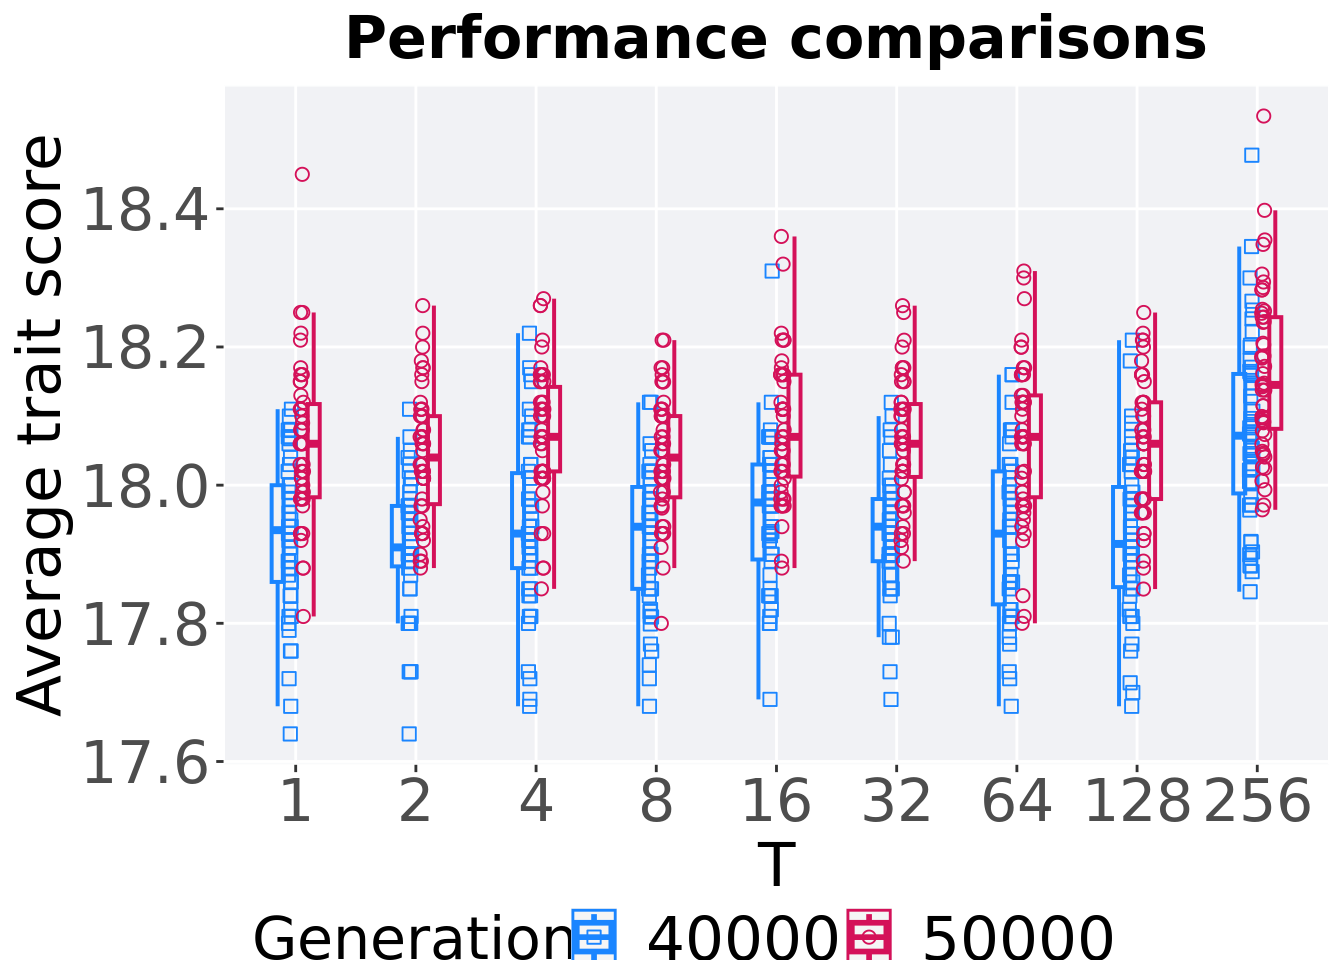
\includegraphics{demo_files/figure-latex/tru-exp-mvc-per-sli-1.pdf}

\hypertarget{stats-23}{%
\subsubsection{Stats}\label{stats-23}}

Summary statistics for the performance of the best performance at 40,000 and 50,000 generations.

\begin{Shaded}
\begin{Highlighting}[]
\NormalTok{slices =}\StringTok{ }\KeywordTok{filter}\NormalTok{(tru_ot_mvc, diagnostic }\OperatorTok{==}\StringTok{ 'exploitation_rate'} \OperatorTok{&}\StringTok{ }\NormalTok{(gen }\OperatorTok{==}\StringTok{ }\DecValTok{50000} \OperatorTok{|}\StringTok{ }\NormalTok{gen }\OperatorTok{==}\StringTok{ }\DecValTok{40000}\NormalTok{))}
\NormalTok{slices}\OperatorTok{$}\NormalTok{Generation <-}\StringTok{ }\KeywordTok{factor}\NormalTok{(slices}\OperatorTok{$}\NormalTok{gen, }\DataTypeTok{levels =} \KeywordTok{c}\NormalTok{(}\DecValTok{50000}\NormalTok{,}\DecValTok{40000}\NormalTok{))}
\NormalTok{slices }\OperatorTok
\StringTok{  }\KeywordTok{group_by}\NormalTok{(T, Generation) }\OperatorTok
\StringTok{  }\NormalTok{dplyr}\OperatorTok{::}\KeywordTok{summarise}\NormalTok{(}
    \DataTypeTok{count =} \KeywordTok{n}\NormalTok{(),}
    \DataTypeTok{na_cnt =} \KeywordTok{sum}\NormalTok{(}\KeywordTok{is.na}\NormalTok{(pop_fit_max  }\OperatorTok{/}\StringTok{ }\NormalTok{DIMENSIONALITY)),}
    \DataTypeTok{min =} \KeywordTok{min}\NormalTok{(pop_fit_max  }\OperatorTok{/}\StringTok{ }\NormalTok{DIMENSIONALITY, }\DataTypeTok{na.rm =} \OtherTok{TRUE}\NormalTok{),}
    \DataTypeTok{median =} \KeywordTok{median}\NormalTok{(pop_fit_max  }\OperatorTok{/}\StringTok{ }\NormalTok{DIMENSIONALITY, }\DataTypeTok{na.rm =} \OtherTok{TRUE}\NormalTok{),}
    \DataTypeTok{mean =} \KeywordTok{mean}\NormalTok{(pop_fit_max  }\OperatorTok{/}\StringTok{ }\NormalTok{DIMENSIONALITY, }\DataTypeTok{na.rm =} \OtherTok{TRUE}\NormalTok{),}
    \DataTypeTok{max =} \KeywordTok{max}\NormalTok{(pop_fit_max  }\OperatorTok{/}\StringTok{ }\NormalTok{DIMENSIONALITY, }\DataTypeTok{na.rm =} \OtherTok{TRUE}\NormalTok{),}
    \DataTypeTok{IQR =} \KeywordTok{IQR}\NormalTok{(pop_fit_max  }\OperatorTok{/}\StringTok{ }\NormalTok{DIMENSIONALITY, }\DataTypeTok{na.rm =} \OtherTok{TRUE}\NormalTok{)}
\NormalTok{  )}
\end{Highlighting}
\end{Shaded}

\begin{verbatim}
## `summarise()` has grouped output by 'T'. You can override using the `.groups`
## argument.
\end{verbatim}

\begin{verbatim}
## # A tibble: 18 x 9
## # Groups:   T [9]
##    T     Generation count na_cnt   min median  mean   max    IQR
##    <fct> <fct>      <int>  <int> <dbl>  <dbl> <dbl> <dbl>  <dbl>
##  1 1     50000         50      0  17.8   18.1  18.1  18.4 0.135 
##  2 1     40000         50      0  17.6   17.9  17.9  18.1 0.140 
##  3 2     50000         50      0  17.9   18.0  18.0  18.3 0.127 
##  4 2     40000         50      0  17.6   17.9  17.9  18.1 0.0875
##  5 4     50000         50      0  17.8   18.1  18.1  18.3 0.122 
##  6 4     40000         50      0  17.7   17.9  17.9  18.2 0.138 
##  7 8     50000         50      0  17.8   18.0  18.0  18.2 0.118 
##  8 8     40000         50      0  17.7   17.9  17.9  18.1 0.147 
##  9 16    50000         50      0  17.9   18.1  18.1  18.4 0.148 
## 10 16    40000         50      0  17.7   18.0  18.0  18.3 0.137 
## 11 32    50000         50      0  17.9   18.1  18.1  18.3 0.106 
## 12 32    40000         50      0  17.7   17.9  17.9  18.1 0.0900
## 13 64    50000         50      0  17.8   18.1  18.1  18.3 0.147 
## 14 64    40000         50      0  17.7   17.9  17.9  18.2 0.192 
## 15 128   50000         50      0  17.8   18.1  18.1  18.2 0.140 
## 16 128   40000         50      0  17.7   17.9  17.9  18.2 0.145 
## 17 256   50000         50      0  18.0   18.1  18.2  18.5 0.162 
## 18 256   40000         50      0  17.8   18.1  18.1  18.5 0.173
\end{verbatim}

T 2

\begin{Shaded}
\begin{Highlighting}[]
\KeywordTok{wilcox.test}\NormalTok{(}\DataTypeTok{x =} \KeywordTok{filter}\NormalTok{(slices, T }\OperatorTok{==}\StringTok{ }\DecValTok{2} \OperatorTok{&}\StringTok{ }\NormalTok{Generation }\OperatorTok{==}\StringTok{ }\DecValTok{50000}\NormalTok{)}\OperatorTok{$}\NormalTok{pop_fit_max,}
            \DataTypeTok{y =} \KeywordTok{filter}\NormalTok{(slices, T }\OperatorTok{==}\StringTok{ }\DecValTok{2} \OperatorTok{&}\StringTok{ }\NormalTok{Generation }\OperatorTok{==}\StringTok{ }\DecValTok{40000}\NormalTok{)}\OperatorTok{$}\NormalTok{pop_fit_max,}
            \DataTypeTok{alternative =} \StringTok{'t'}\NormalTok{)}
\end{Highlighting}
\end{Shaded}

\begin{verbatim}
## 
##  Wilcoxon rank sum test with continuity correction
## 
## data:  filter(slices, T == 2 & Generation == 50000)$pop_fit_max and filter(slices, T == 2 & Generation == 40000)$pop_fit_max
## W = 2109.5, p-value = 3.13e-09
## alternative hypothesis: true location shift is not equal to 0
\end{verbatim}

T 4

\begin{Shaded}
\begin{Highlighting}[]
\KeywordTok{wilcox.test}\NormalTok{(}\DataTypeTok{x =} \KeywordTok{filter}\NormalTok{(slices, T }\OperatorTok{==}\StringTok{ }\DecValTok{4} \OperatorTok{&}\StringTok{ }\NormalTok{Generation }\OperatorTok{==}\StringTok{ }\DecValTok{50000}\NormalTok{)}\OperatorTok{$}\NormalTok{pop_fit_max,}
            \DataTypeTok{y =} \KeywordTok{filter}\NormalTok{(slices, T }\OperatorTok{==}\StringTok{ }\DecValTok{4} \OperatorTok{&}\StringTok{ }\NormalTok{Generation }\OperatorTok{==}\StringTok{ }\DecValTok{40000}\NormalTok{)}\OperatorTok{$}\NormalTok{pop_fit_max,}
            \DataTypeTok{alternative =} \StringTok{'t'}\NormalTok{)}
\end{Highlighting}
\end{Shaded}

\begin{verbatim}
## 
##  Wilcoxon rank sum test with continuity correction
## 
## data:  filter(slices, T == 4 & Generation == 50000)$pop_fit_max and filter(slices, T == 4 & Generation == 40000)$pop_fit_max
## W = 2003.5, p-value = 2.067e-07
## alternative hypothesis: true location shift is not equal to 0
\end{verbatim}

T 8

\begin{Shaded}
\begin{Highlighting}[]
\KeywordTok{wilcox.test}\NormalTok{(}\DataTypeTok{x =} \KeywordTok{filter}\NormalTok{(slices, T }\OperatorTok{==}\StringTok{ }\DecValTok{8} \OperatorTok{&}\StringTok{ }\NormalTok{Generation }\OperatorTok{==}\StringTok{ }\DecValTok{50000}\NormalTok{)}\OperatorTok{$}\NormalTok{pop_fit_max,}
            \DataTypeTok{y =} \KeywordTok{filter}\NormalTok{(slices, T }\OperatorTok{==}\StringTok{ }\DecValTok{8} \OperatorTok{&}\StringTok{ }\NormalTok{Generation }\OperatorTok{==}\StringTok{ }\DecValTok{40000}\NormalTok{)}\OperatorTok{$}\NormalTok{pop_fit_max,}
            \DataTypeTok{alternative =} \StringTok{'t'}\NormalTok{)}
\end{Highlighting}
\end{Shaded}

\begin{verbatim}
## 
##  Wilcoxon rank sum test with continuity correction
## 
## data:  filter(slices, T == 8 & Generation == 50000)$pop_fit_max and filter(slices, T == 8 & Generation == 40000)$pop_fit_max
## W = 2037.5, p-value = 5.705e-08
## alternative hypothesis: true location shift is not equal to 0
\end{verbatim}

T 16

\begin{Shaded}
\begin{Highlighting}[]
\KeywordTok{wilcox.test}\NormalTok{(}\DataTypeTok{x =} \KeywordTok{filter}\NormalTok{(slices, T }\OperatorTok{==}\StringTok{ }\DecValTok{16} \OperatorTok{&}\StringTok{ }\NormalTok{Generation }\OperatorTok{==}\StringTok{ }\DecValTok{50000}\NormalTok{)}\OperatorTok{$}\NormalTok{pop_fit_max,}
            \DataTypeTok{y =} \KeywordTok{filter}\NormalTok{(slices, T }\OperatorTok{==}\StringTok{ }\DecValTok{16} \OperatorTok{&}\StringTok{ }\NormalTok{Generation }\OperatorTok{==}\StringTok{ }\DecValTok{40000}\NormalTok{)}\OperatorTok{$}\NormalTok{pop_fit_max,}
            \DataTypeTok{alternative =} \StringTok{'t'}\NormalTok{)}
\end{Highlighting}
\end{Shaded}

\begin{verbatim}
## 
##  Wilcoxon rank sum test with continuity correction
## 
## data:  filter(slices, T == 16 & Generation == 50000)$pop_fit_max and filter(slices, T == 16 & Generation == 40000)$pop_fit_max
## W = 1998.5, p-value = 2.457e-07
## alternative hypothesis: true location shift is not equal to 0
\end{verbatim}

T 32

\begin{Shaded}
\begin{Highlighting}[]
\KeywordTok{wilcox.test}\NormalTok{(}\DataTypeTok{x =} \KeywordTok{filter}\NormalTok{(slices, T }\OperatorTok{==}\StringTok{ }\DecValTok{32} \OperatorTok{&}\StringTok{ }\NormalTok{Generation }\OperatorTok{==}\StringTok{ }\DecValTok{50000}\NormalTok{)}\OperatorTok{$}\NormalTok{pop_fit_max,}
            \DataTypeTok{y =} \KeywordTok{filter}\NormalTok{(slices, T }\OperatorTok{==}\StringTok{ }\DecValTok{32} \OperatorTok{&}\StringTok{ }\NormalTok{Generation }\OperatorTok{==}\StringTok{ }\DecValTok{40000}\NormalTok{)}\OperatorTok{$}\NormalTok{pop_fit_max,}
            \DataTypeTok{alternative =} \StringTok{'t'}\NormalTok{)}
\end{Highlighting}
\end{Shaded}

\begin{verbatim}
## 
##  Wilcoxon rank sum test with continuity correction
## 
## data:  filter(slices, T == 32 & Generation == 50000)$pop_fit_max and filter(slices, T == 32 & Generation == 40000)$pop_fit_max
## W = 2151, p-value = 5.311e-10
## alternative hypothesis: true location shift is not equal to 0
\end{verbatim}

T 64

\begin{Shaded}
\begin{Highlighting}[]
\KeywordTok{wilcox.test}\NormalTok{(}\DataTypeTok{x =} \KeywordTok{filter}\NormalTok{(slices, T }\OperatorTok{==}\StringTok{ }\DecValTok{64} \OperatorTok{&}\StringTok{ }\NormalTok{Generation }\OperatorTok{==}\StringTok{ }\DecValTok{50000}\NormalTok{)}\OperatorTok{$}\NormalTok{pop_fit_max,}
            \DataTypeTok{y =} \KeywordTok{filter}\NormalTok{(slices, T }\OperatorTok{==}\StringTok{ }\DecValTok{64} \OperatorTok{&}\StringTok{ }\NormalTok{Generation }\OperatorTok{==}\StringTok{ }\DecValTok{40000}\NormalTok{)}\OperatorTok{$}\NormalTok{pop_fit_max,}
            \DataTypeTok{alternative =} \StringTok{'t'}\NormalTok{)}
\end{Highlighting}
\end{Shaded}

\begin{verbatim}
## 
##  Wilcoxon rank sum test with continuity correction
## 
## data:  filter(slices, T == 64 & Generation == 50000)$pop_fit_max and filter(slices, T == 64 & Generation == 40000)$pop_fit_max
## W = 1997, p-value = 2.628e-07
## alternative hypothesis: true location shift is not equal to 0
\end{verbatim}

T 128

\begin{Shaded}
\begin{Highlighting}[]
\KeywordTok{wilcox.test}\NormalTok{(}\DataTypeTok{x =} \KeywordTok{filter}\NormalTok{(slices, T }\OperatorTok{==}\StringTok{ }\DecValTok{128} \OperatorTok{&}\StringTok{ }\NormalTok{Generation }\OperatorTok{==}\StringTok{ }\DecValTok{50000}\NormalTok{)}\OperatorTok{$}\NormalTok{pop_fit_max,}
            \DataTypeTok{y =} \KeywordTok{filter}\NormalTok{(slices, T }\OperatorTok{==}\StringTok{ }\DecValTok{128} \OperatorTok{&}\StringTok{ }\NormalTok{Generation }\OperatorTok{==}\StringTok{ }\DecValTok{40000}\NormalTok{)}\OperatorTok{$}\NormalTok{pop_fit_max,}
            \DataTypeTok{alternative =} \StringTok{'t'}\NormalTok{)}
\end{Highlighting}
\end{Shaded}

\begin{verbatim}
## 
##  Wilcoxon rank sum test with continuity correction
## 
## data:  filter(slices, T == 128 & Generation == 50000)$pop_fit_max and filter(slices, T == 128 & Generation == 40000)$pop_fit_max
## W = 2022.5, p-value = 1.009e-07
## alternative hypothesis: true location shift is not equal to 0
\end{verbatim}

T 256

\begin{Shaded}
\begin{Highlighting}[]
\KeywordTok{wilcox.test}\NormalTok{(}\DataTypeTok{x =} \KeywordTok{filter}\NormalTok{(slices, T }\OperatorTok{==}\StringTok{ }\DecValTok{256} \OperatorTok{&}\StringTok{ }\NormalTok{Generation }\OperatorTok{==}\StringTok{ }\DecValTok{50000}\NormalTok{)}\OperatorTok{$}\NormalTok{pop_fit_max,}
            \DataTypeTok{y =} \KeywordTok{filter}\NormalTok{(slices, T }\OperatorTok{==}\StringTok{ }\DecValTok{256} \OperatorTok{&}\StringTok{ }\NormalTok{Generation }\OperatorTok{==}\StringTok{ }\DecValTok{40000}\NormalTok{)}\OperatorTok{$}\NormalTok{pop_fit_max,}
            \DataTypeTok{alternative =} \StringTok{'t'}\NormalTok{)}
\end{Highlighting}
\end{Shaded}

\begin{verbatim}
## 
##  Wilcoxon rank sum test with continuity correction
## 
## data:  filter(slices, T == 256 & Generation == 50000)$pop_fit_max and filter(slices, T == 256 & Generation == 40000)$pop_fit_max
## W = 1742, p-value = 0.0007032
## alternative hypothesis: true location shift is not equal to 0
\end{verbatim}

\hypertarget{ordered-exploitation-results-1}{%
\section{Ordered exploitation results}\label{ordered-exploitation-results-1}}

Here we present the results for \textbf{best performances} found by each truncation selection size value replicate on the ordered exploitation diagnostic.
Best performance found refers to the largest average trait score found in a given population.
Note that performance values fall between 0 and 100.

\hypertarget{performance-over-time-7}{%
\subsection{Performance over time}\label{performance-over-time-7}}

Performance over time.

\begin{Shaded}
\begin{Highlighting}[]
\NormalTok{lines =}\StringTok{ }\KeywordTok{filter}\NormalTok{(tru_ot, diagnostic }\OperatorTok{==}\StringTok{ 'ordered_exploitation'}\NormalTok{) }\OperatorTok
\StringTok{        }\KeywordTok{group_by}\NormalTok{(T, gen) }\OperatorTok
\StringTok{          }\NormalTok{dplyr}\OperatorTok{::}\KeywordTok{summarise}\NormalTok{(}
            \DataTypeTok{min =} \KeywordTok{min}\NormalTok{(pop_fit_max),}
            \DataTypeTok{mean =} \KeywordTok{mean}\NormalTok{(pop_fit_max),}
            \DataTypeTok{max =} \KeywordTok{max}\NormalTok{(pop_fit_max)}
\NormalTok{          )}
\end{Highlighting}
\end{Shaded}

\begin{verbatim}
## `summarise()` has grouped output by 'T'. You can override using the `.groups`
## argument.
\end{verbatim}

\begin{Shaded}
\begin{Highlighting}[]
\KeywordTok{ggplot}\NormalTok{(lines, }\KeywordTok{aes}\NormalTok{(}\DataTypeTok{x=}\NormalTok{gen, }\DataTypeTok{y=}\NormalTok{mean }\OperatorTok{/}\StringTok{ }\NormalTok{DIMENSIONALITY, }\DataTypeTok{group =}\NormalTok{ T, }\DataTypeTok{fill =}\NormalTok{ T, }\DataTypeTok{color =}\NormalTok{ T, }\DataTypeTok{shape =}\NormalTok{ T)) }\OperatorTok{+}
\StringTok{  }\KeywordTok{geom_ribbon}\NormalTok{(}\KeywordTok{aes}\NormalTok{(}\DataTypeTok{ymin =}\NormalTok{ min }\OperatorTok{/}\StringTok{ }\NormalTok{DIMENSIONALITY, }\DataTypeTok{ymax =}\NormalTok{ max }\OperatorTok{/}\StringTok{ }\NormalTok{DIMENSIONALITY), }\DataTypeTok{alpha =} \FloatTok{0.1}\NormalTok{) }\OperatorTok{+}
\StringTok{  }\KeywordTok{geom_line}\NormalTok{(}\DataTypeTok{size =} \FloatTok{0.5}\NormalTok{) }\OperatorTok{+}
\StringTok{  }\KeywordTok{geom_point}\NormalTok{(}\DataTypeTok{data =} \KeywordTok{filter}\NormalTok{(lines, gen }\OperatorTok\StringTok{ }\DecValTok{2000} \OperatorTok{==}\StringTok{ }\DecValTok{0} \OperatorTok{&}\StringTok{ }\NormalTok{gen }\OperatorTok{!=}\StringTok{ }\DecValTok{0}\NormalTok{), }\DataTypeTok{size =} \FloatTok{1.5}\NormalTok{, }\DataTypeTok{stroke =} \FloatTok{2.0}\NormalTok{, }\DataTypeTok{alpha =} \FloatTok{1.0}\NormalTok{) }\OperatorTok{+}
\StringTok{  }\KeywordTok{scale_y_continuous}\NormalTok{(}
    \DataTypeTok{name=}\StringTok{"Average trait score"}\NormalTok{,}
    \DataTypeTok{limits=}\KeywordTok{c}\NormalTok{(}\OperatorTok{-}\DecValTok{1}\NormalTok{, }\DecValTok{101}\NormalTok{),}
    \DataTypeTok{breaks=}\KeywordTok{seq}\NormalTok{(}\DecValTok{0}\NormalTok{,}\DecValTok{100}\NormalTok{, }\DecValTok{20}\NormalTok{),}
    \DataTypeTok{labels=}\KeywordTok{c}\NormalTok{(}\StringTok{"0"}\NormalTok{, }\StringTok{"20"}\NormalTok{, }\StringTok{"40"}\NormalTok{, }\StringTok{"60"}\NormalTok{, }\StringTok{"80"}\NormalTok{, }\StringTok{"100"}\NormalTok{)}
\NormalTok{  ) }\OperatorTok{+}
\StringTok{  }\KeywordTok{scale_x_continuous}\NormalTok{(}
    \DataTypeTok{name=}\StringTok{"Generations"}\NormalTok{,}
    \DataTypeTok{limits=}\KeywordTok{c}\NormalTok{(}\DecValTok{0}\NormalTok{, }\DecValTok{50000}\NormalTok{),}
    \DataTypeTok{breaks=}\KeywordTok{c}\NormalTok{(}\DecValTok{0}\NormalTok{, }\DecValTok{10000}\NormalTok{, }\DecValTok{20000}\NormalTok{, }\DecValTok{30000}\NormalTok{, }\DecValTok{40000}\NormalTok{, }\DecValTok{50000}\NormalTok{),}
    \DataTypeTok{labels=}\KeywordTok{c}\NormalTok{(}\StringTok{"0e+4"}\NormalTok{, }\StringTok{"1e+4"}\NormalTok{, }\StringTok{"2e+4"}\NormalTok{, }\StringTok{"3e+4"}\NormalTok{, }\StringTok{"4e+4"}\NormalTok{, }\StringTok{"5e+4"}\NormalTok{)}

\NormalTok{  ) }\OperatorTok{+}
\StringTok{  }\KeywordTok{scale_shape_manual}\NormalTok{(}\DataTypeTok{values=}\NormalTok{SHAPE)}\OperatorTok{+}
\StringTok{  }\KeywordTok{scale_colour_manual}\NormalTok{(}\DataTypeTok{values =}\NormalTok{ cb_palette) }\OperatorTok{+}
\StringTok{  }\KeywordTok{scale_fill_manual}\NormalTok{(}\DataTypeTok{values =}\NormalTok{ cb_palette) }\OperatorTok{+}
\StringTok{  }\KeywordTok{ggtitle}\NormalTok{(}\StringTok{"Best performance over time"}\NormalTok{) }\OperatorTok{+}
\StringTok{  }\NormalTok{p_theme}
\end{Highlighting}
\end{Shaded}

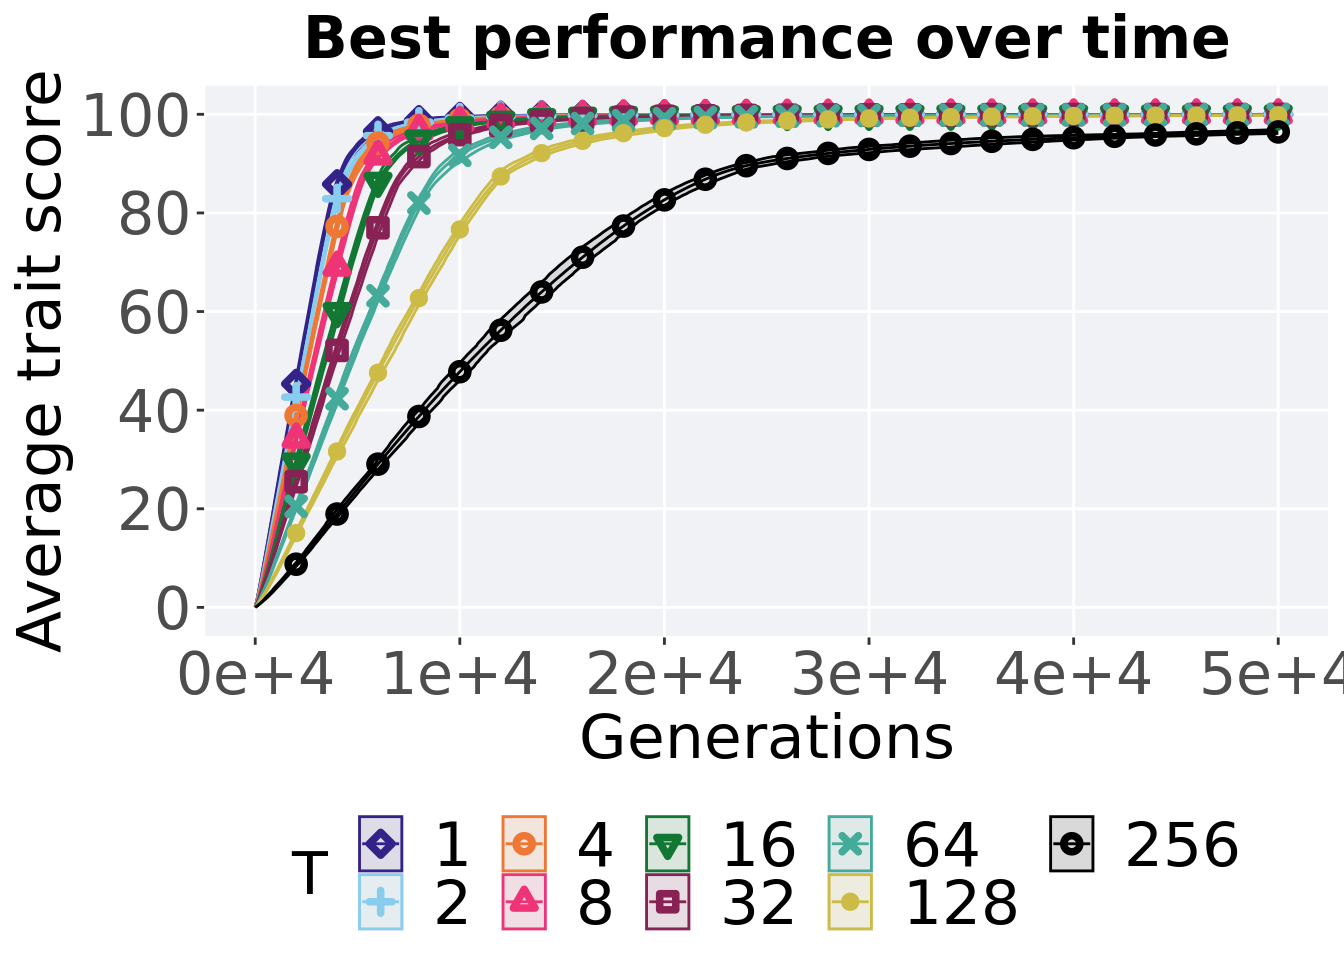
\includegraphics{demo_files/figure-latex/tru-ord-per-1.pdf}

\hypertarget{generation-satisfactory-solution-found-3}{%
\subsection{Generation satisfactory solution found}\label{generation-satisfactory-solution-found-3}}

The first Generations a satisfactory solution is found throughout the 50,000 generations.

\begin{Shaded}
\begin{Highlighting}[]
\KeywordTok{filter}\NormalTok{(tru_ssf, Diagnostic }\OperatorTok{==}\StringTok{ 'ORDERED_EXPLOITATION'}\NormalTok{) }\OperatorTok
\KeywordTok{ggplot}\NormalTok{(., }\KeywordTok{aes}\NormalTok{(}\DataTypeTok{x =}\NormalTok{ T, }\DataTypeTok{y =}\NormalTok{ Generations, }\DataTypeTok{color =}\NormalTok{ T, }\DataTypeTok{fill =}\NormalTok{ T, }\DataTypeTok{shape =}\NormalTok{ T)) }\OperatorTok{+}
\StringTok{  }\KeywordTok{geom_flat_violin}\NormalTok{(}\DataTypeTok{position =} \KeywordTok{position_nudge}\NormalTok{(}\DataTypeTok{x =} \FloatTok{.2}\NormalTok{, }\DataTypeTok{y =} \DecValTok{0}\NormalTok{), }\DataTypeTok{scale =} \StringTok{'width'}\NormalTok{, }\DataTypeTok{alpha =} \FloatTok{0.2}\NormalTok{) }\OperatorTok{+}
\StringTok{  }\KeywordTok{geom_point}\NormalTok{(}\DataTypeTok{position =} \KeywordTok{position_jitter}\NormalTok{(}\DataTypeTok{width =} \FloatTok{.1}\NormalTok{), }\DataTypeTok{size =} \FloatTok{1.5}\NormalTok{, }\DataTypeTok{alpha =} \FloatTok{1.0}\NormalTok{) }\OperatorTok{+}
\StringTok{  }\KeywordTok{geom_boxplot}\NormalTok{(}\DataTypeTok{color =} \StringTok{'black'}\NormalTok{, }\DataTypeTok{width =} \FloatTok{.2}\NormalTok{, }\DataTypeTok{outlier.shape =} \OtherTok{NA}\NormalTok{, }\DataTypeTok{alpha =} \FloatTok{0.0}\NormalTok{) }\OperatorTok{+}
\StringTok{  }\KeywordTok{scale_shape_manual}\NormalTok{(}\DataTypeTok{values=}\NormalTok{SHAPE)}\OperatorTok{+}
\StringTok{  }\KeywordTok{scale_y_continuous}\NormalTok{(}
    \DataTypeTok{name=}\StringTok{"Generation"}\NormalTok{,}
    \DataTypeTok{limits=}\KeywordTok{c}\NormalTok{(}\DecValTok{0}\NormalTok{, }\DecValTok{60000}\NormalTok{),}
    \DataTypeTok{breaks=}\KeywordTok{c}\NormalTok{(}\DecValTok{0}\NormalTok{, }\DecValTok{10000}\NormalTok{, }\DecValTok{20000}\NormalTok{, }\DecValTok{30000}\NormalTok{, }\DecValTok{40000}\NormalTok{, }\DecValTok{50000}\NormalTok{, }\DecValTok{60000}\NormalTok{),}
    \DataTypeTok{labels=}\KeywordTok{c}\NormalTok{(}\StringTok{"0e+4"}\NormalTok{, }\StringTok{"1e+4"}\NormalTok{, }\StringTok{"2e+4"}\NormalTok{, }\StringTok{"3e+4"}\NormalTok{, }\StringTok{"4e+4"}\NormalTok{, }\StringTok{"5e+4"}\NormalTok{, }\StringTok{"Fail"}\NormalTok{)}
\NormalTok{  ) }\OperatorTok{+}
\StringTok{  }\KeywordTok{scale_x_discrete}\NormalTok{(}
    \DataTypeTok{name=}\StringTok{"T"}
\NormalTok{  ) }\OperatorTok{+}
\StringTok{  }\KeywordTok{scale_colour_manual}\NormalTok{(}\DataTypeTok{values =}\NormalTok{ cb_palette) }\OperatorTok{+}
\StringTok{  }\KeywordTok{scale_fill_manual}\NormalTok{(}\DataTypeTok{values =}\NormalTok{ cb_palette) }\OperatorTok{+}
\StringTok{  }\KeywordTok{ggtitle}\NormalTok{(}\StringTok{"Generation satisfactory solution found"}\NormalTok{) }\OperatorTok{+}
\StringTok{  }\NormalTok{p_theme}
\end{Highlighting}
\end{Shaded}

\begin{verbatim}
## Warning: Removed 34 rows containing missing values (`geom_point()`).
\end{verbatim}

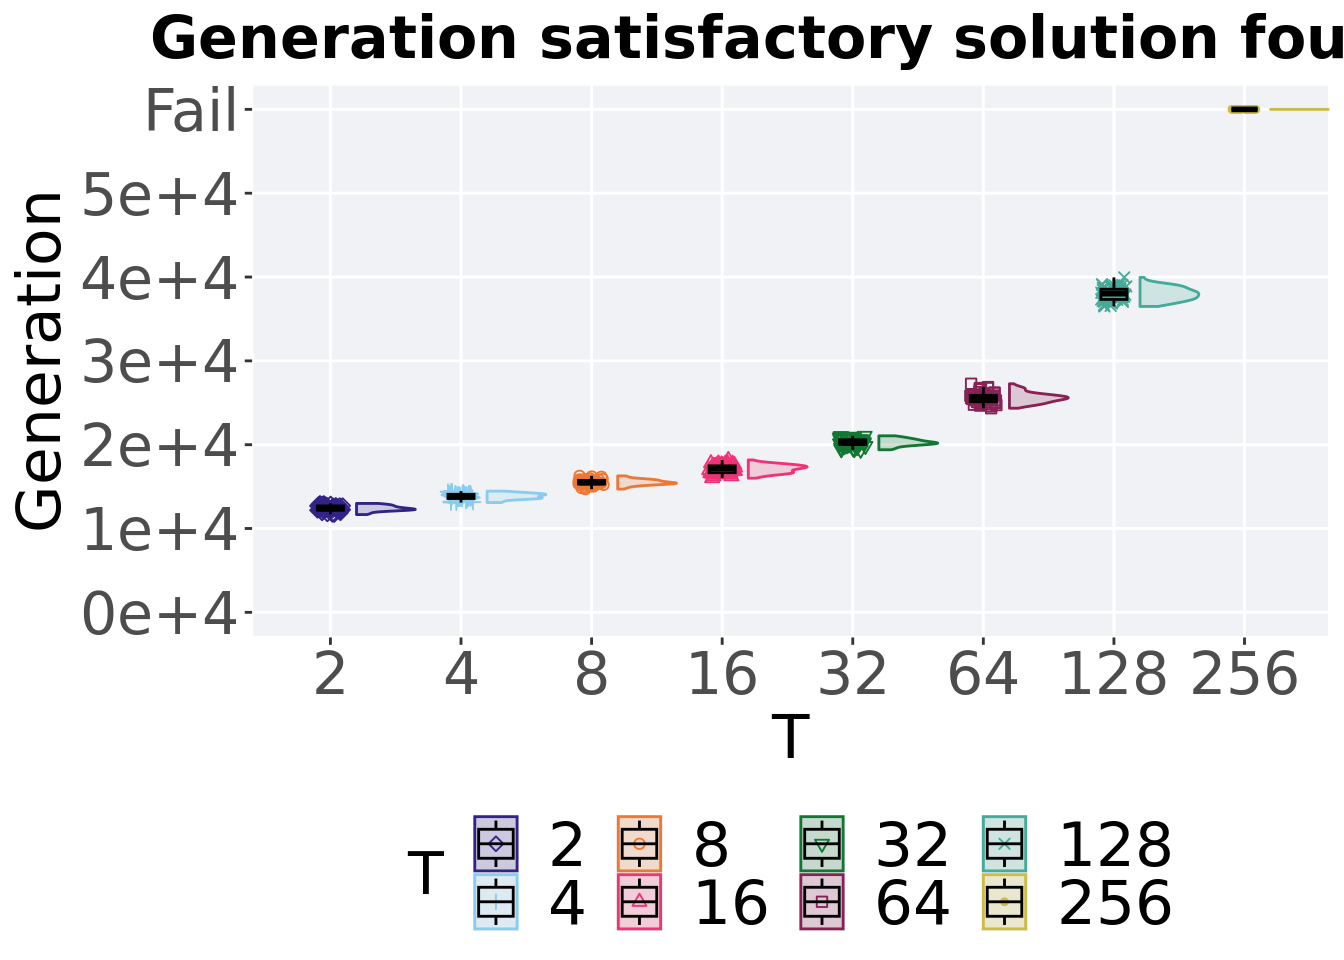
\includegraphics{demo_files/figure-latex/tru-ord-ssf-1.pdf}

\hypertarget{stats-24}{%
\subsubsection{Stats}\label{stats-24}}

Summary statistics for the first Generations a satisfactory solution is found throughout the 50,000 generations.

\begin{Shaded}
\begin{Highlighting}[]
\NormalTok{ssf =}\StringTok{ }\KeywordTok{filter}\NormalTok{(tru_ssf, Diagnostic }\OperatorTok{==}\StringTok{ 'ORDERED_EXPLOITATION'}\NormalTok{)}
\KeywordTok{group_by}\NormalTok{(ssf, T) }\OperatorTok
\StringTok{  }\NormalTok{dplyr}\OperatorTok{::}\KeywordTok{summarise}\NormalTok{(}
    \DataTypeTok{count =} \KeywordTok{n}\NormalTok{(),}
    \DataTypeTok{na_cnt =} \KeywordTok{sum}\NormalTok{(}\KeywordTok{is.na}\NormalTok{(Generations)),}
    \DataTypeTok{min =} \KeywordTok{min}\NormalTok{(Generations, }\DataTypeTok{na.rm =} \OtherTok{TRUE}\NormalTok{),}
    \DataTypeTok{median =} \KeywordTok{median}\NormalTok{(Generations, }\DataTypeTok{na.rm =} \OtherTok{TRUE}\NormalTok{),}
    \DataTypeTok{mean =} \KeywordTok{mean}\NormalTok{(Generations, }\DataTypeTok{na.rm =} \OtherTok{TRUE}\NormalTok{),}
    \DataTypeTok{max =} \KeywordTok{max}\NormalTok{(Generations, }\DataTypeTok{na.rm =} \OtherTok{TRUE}\NormalTok{),}
    \DataTypeTok{IQR =} \KeywordTok{IQR}\NormalTok{(Generations, }\DataTypeTok{na.rm =} \OtherTok{TRUE}\NormalTok{)}
\NormalTok{  )}
\end{Highlighting}
\end{Shaded}

\begin{verbatim}
## # A tibble: 8 x 8
##   T     count na_cnt   min median   mean   max   IQR
##   <fct> <int>  <int> <int>  <dbl>  <dbl> <int> <dbl>
## 1 2        50      0 11664 12356. 12407. 12992  496.
## 2 4        50      0 13096 13871  13840. 14459  496.
## 3 8        50      0 14701 15466. 15511. 16280  422.
## 4 16       50      0 16002 17192  17098. 18174  813.
## 5 32       50      0 19392 20223  20274. 21055  555.
## 6 64       50      0 24348 25568. 25598. 27268  764.
## 7 128      50      0 36490 38016  37967. 39959 1210.
## 8 256      50      0 60000 60000  60000  60000    0
\end{verbatim}

Kruskal--Wallis test provides evidence of significant differences among the first Generations a satisfactory solution is found throughout the 50,000 generations.

\begin{Shaded}
\begin{Highlighting}[]
\KeywordTok{kruskal.test}\NormalTok{(Generations }\OperatorTok{~}\StringTok{ }\NormalTok{T, }\DataTypeTok{data =}\NormalTok{ ssf)}
\end{Highlighting}
\end{Shaded}

\begin{verbatim}
## 
##  Kruskal-Wallis rank sum test
## 
## data:  Generations by T
## Kruskal-Wallis chi-squared = 393.49, df = 7, p-value < 2.2e-16
\end{verbatim}

Results for post-hoc Wilcoxon rank-sum test with a Bonferroni correction on the first Generations a satisfactory solution is found throughout the 50,000 generations.

\begin{Shaded}
\begin{Highlighting}[]
\KeywordTok{pairwise.wilcox.test}\NormalTok{(}\DataTypeTok{x =}\NormalTok{ ssf}\OperatorTok{$}\NormalTok{Generations, }\DataTypeTok{g =}\NormalTok{ ssf}\OperatorTok{$}\NormalTok{T , }\DataTypeTok{p.adjust.method =} \StringTok{"bonferroni"}\NormalTok{,}
                     \DataTypeTok{paired =} \OtherTok{FALSE}\NormalTok{, }\DataTypeTok{conf.int =} \OtherTok{FALSE}\NormalTok{, }\DataTypeTok{alternative =} \StringTok{'g'}\NormalTok{)}
\end{Highlighting}
\end{Shaded}

\begin{verbatim}
## 
##  Pairwise comparisons using Wilcoxon rank sum test with continuity correction 
## 
## data:  ssf$Generations and ssf$T 
## 
##     2      4      8      16     32     64     128   
## 4   <2e-16 -      -      -      -      -      -     
## 8   <2e-16 <2e-16 -      -      -      -      -     
## 16  <2e-16 <2e-16 <2e-16 -      -      -      -     
## 32  <2e-16 <2e-16 <2e-16 <2e-16 -      -      -     
## 64  <2e-16 <2e-16 <2e-16 <2e-16 <2e-16 -      -     
## 128 <2e-16 <2e-16 <2e-16 <2e-16 <2e-16 <2e-16 -     
## 256 <2e-16 <2e-16 <2e-16 <2e-16 <2e-16 <2e-16 <2e-16
## 
## P value adjustment method: bonferroni
\end{verbatim}

\hypertarget{multi-valley-crossing-1}{%
\subsection{Multi-valley crossing}\label{multi-valley-crossing-1}}

\hypertarget{performance-over-time-8}{%
\subsubsection{Performance over time}\label{performance-over-time-8}}

\begin{Shaded}
\begin{Highlighting}[]
\CommentTok{# data for lines and shading on plots}
\NormalTok{lines =}\StringTok{ }\KeywordTok{filter}\NormalTok{(tru_ot_mvc, diagnostic }\OperatorTok{==}\StringTok{ 'ordered_exploitation'}\NormalTok{) }\OperatorTok
\StringTok{  }\KeywordTok{group_by}\NormalTok{(T, gen) }\OperatorTok
\StringTok{  }\NormalTok{dplyr}\OperatorTok{::}\KeywordTok{summarise}\NormalTok{(}
    \DataTypeTok{min =} \KeywordTok{min}\NormalTok{(pop_fit_max) }\OperatorTok{/}\StringTok{ }\NormalTok{DIMENSIONALITY,}
    \DataTypeTok{mean =} \KeywordTok{mean}\NormalTok{(pop_fit_max) }\OperatorTok{/}\StringTok{ }\NormalTok{DIMENSIONALITY,}
    \DataTypeTok{max =} \KeywordTok{max}\NormalTok{(pop_fit_max) }\OperatorTok{/}\StringTok{ }\NormalTok{DIMENSIONALITY}
\NormalTok{  )}
\end{Highlighting}
\end{Shaded}

\begin{verbatim}
## `summarise()` has grouped output by 'T'. You can override using the `.groups`
## argument.
\end{verbatim}

\begin{Shaded}
\begin{Highlighting}[]
\KeywordTok{ggplot}\NormalTok{(lines, }\KeywordTok{aes}\NormalTok{(}\DataTypeTok{x=}\NormalTok{gen, }\DataTypeTok{y=}\NormalTok{mean, }\DataTypeTok{group =}\NormalTok{ T, }\DataTypeTok{fill =}\NormalTok{T, }\DataTypeTok{color =}\NormalTok{ T, }\DataTypeTok{shape =}\NormalTok{ T)) }\OperatorTok{+}
\StringTok{  }\KeywordTok{geom_ribbon}\NormalTok{(}\KeywordTok{aes}\NormalTok{(}\DataTypeTok{ymin =}\NormalTok{ min, }\DataTypeTok{ymax =}\NormalTok{ max), }\DataTypeTok{alpha =} \FloatTok{0.1}\NormalTok{) }\OperatorTok{+}
\StringTok{  }\KeywordTok{geom_line}\NormalTok{(}\DataTypeTok{size =} \FloatTok{0.5}\NormalTok{) }\OperatorTok{+}
\StringTok{  }\KeywordTok{geom_point}\NormalTok{(}\DataTypeTok{data =} \KeywordTok{filter}\NormalTok{(lines, gen }\OperatorTok\StringTok{ }\DecValTok{2000} \OperatorTok{==}\StringTok{ }\DecValTok{0} \OperatorTok{&}\StringTok{ }\NormalTok{gen }\OperatorTok{!=}\StringTok{ }\DecValTok{0}\NormalTok{), }\DataTypeTok{size =} \FloatTok{1.5}\NormalTok{, }\DataTypeTok{stroke =} \FloatTok{2.0}\NormalTok{, }\DataTypeTok{alpha =} \FloatTok{1.0}\NormalTok{) }\OperatorTok{+}
\StringTok{  }\KeywordTok{scale_y_continuous}\NormalTok{(}
    \DataTypeTok{name=}\StringTok{"Average trait score"}
\NormalTok{  ) }\OperatorTok{+}
\StringTok{  }\KeywordTok{scale_x_continuous}\NormalTok{(}
    \DataTypeTok{name=}\StringTok{"Generations"}\NormalTok{,}
    \DataTypeTok{limits=}\KeywordTok{c}\NormalTok{(}\DecValTok{0}\NormalTok{, }\DecValTok{50000}\NormalTok{),}
    \DataTypeTok{breaks=}\KeywordTok{c}\NormalTok{(}\DecValTok{0}\NormalTok{, }\DecValTok{10000}\NormalTok{, }\DecValTok{20000}\NormalTok{, }\DecValTok{30000}\NormalTok{, }\DecValTok{40000}\NormalTok{, }\DecValTok{50000}\NormalTok{),}
    \DataTypeTok{labels=}\KeywordTok{c}\NormalTok{(}\StringTok{"0e+4"}\NormalTok{, }\StringTok{"1e+4"}\NormalTok{, }\StringTok{"2e+4"}\NormalTok{, }\StringTok{"3e+4"}\NormalTok{, }\StringTok{"4e+4"}\NormalTok{, }\StringTok{"5e+4"}\NormalTok{)}

\NormalTok{  ) }\OperatorTok{+}
\StringTok{  }\KeywordTok{scale_shape_manual}\NormalTok{(}\DataTypeTok{values=}\NormalTok{SHAPE)}\OperatorTok{+}
\StringTok{  }\KeywordTok{scale_colour_manual}\NormalTok{(}\DataTypeTok{values =}\NormalTok{ cb_palette) }\OperatorTok{+}
\StringTok{  }\KeywordTok{scale_fill_manual}\NormalTok{(}\DataTypeTok{values =}\NormalTok{ cb_palette) }\OperatorTok{+}
\StringTok{  }\KeywordTok{ggtitle}\NormalTok{(}\StringTok{'Performance over time'}\NormalTok{)}\OperatorTok{+}
\StringTok{  }\NormalTok{p_theme }\OperatorTok{+}
\StringTok{  }\KeywordTok{guides}\NormalTok{(}
    \DataTypeTok{shape=}\KeywordTok{guide_legend}\NormalTok{(}\DataTypeTok{nrow=}\DecValTok{2}\NormalTok{, }\DataTypeTok{title.position =} \StringTok{"left"}\NormalTok{),}
    \DataTypeTok{color=}\KeywordTok{guide_legend}\NormalTok{(}\DataTypeTok{nrow=}\DecValTok{2}\NormalTok{, }\DataTypeTok{title.position =} \StringTok{"left"}\NormalTok{),}
    \DataTypeTok{fill=}\KeywordTok{guide_legend}\NormalTok{(}\DataTypeTok{nrow=}\DecValTok{2}\NormalTok{, }\DataTypeTok{title.position =} \StringTok{"left"}\NormalTok{)}
\NormalTok{  )}
\end{Highlighting}
\end{Shaded}

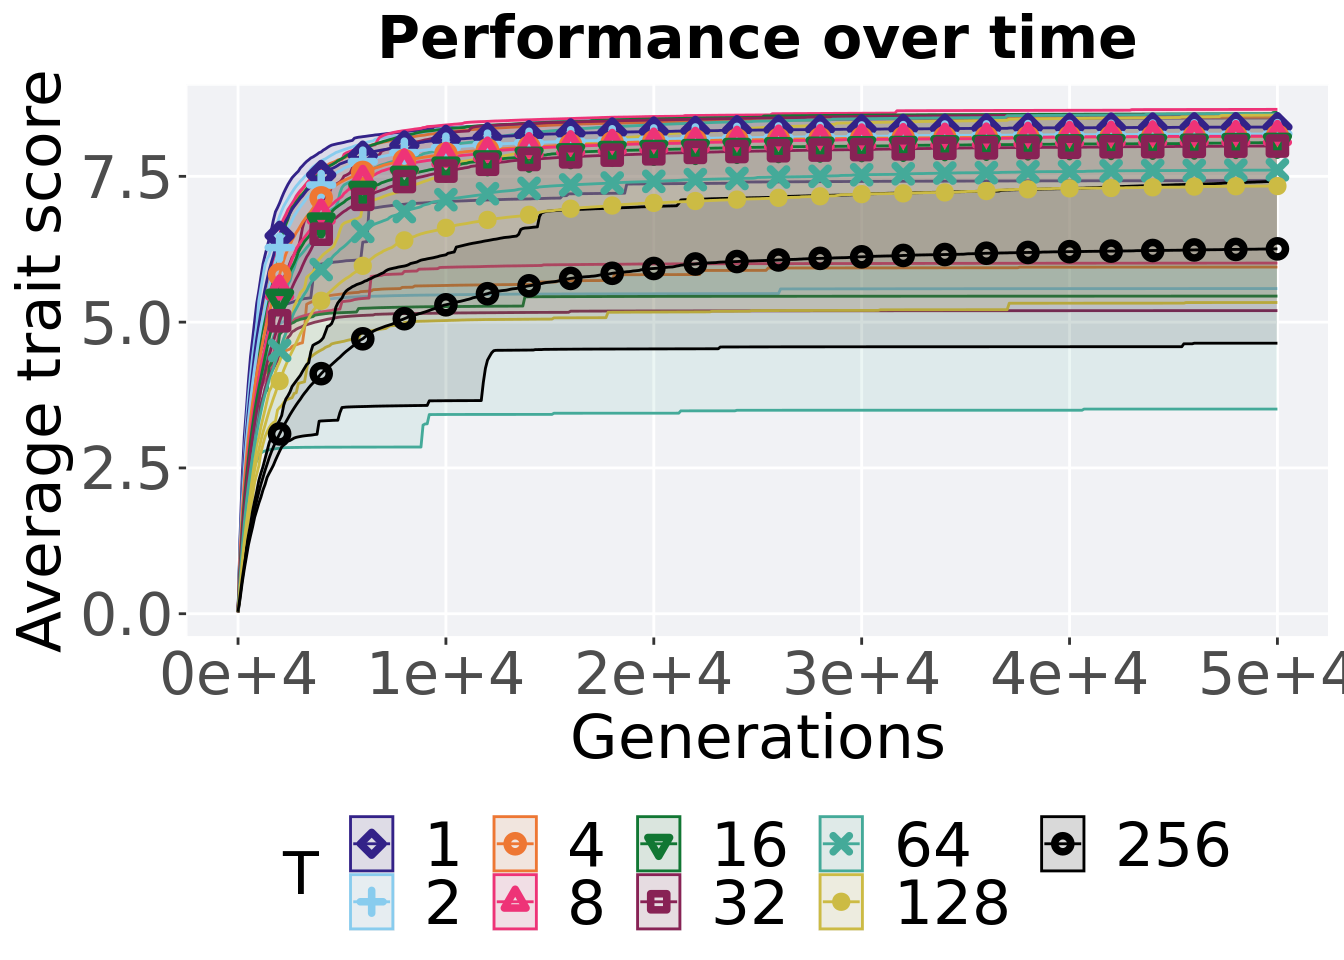
\includegraphics{demo_files/figure-latex/tru-ord-mvc-per-1.pdf}

\hypertarget{performance-comparison-4}{%
\subsubsection{Performance comparison}\label{performance-comparison-4}}

Best performances in the population at 40,000 and 50,000 generations.

\begin{Shaded}
\begin{Highlighting}[]
\CommentTok{# 80% and final generation comparison}
\NormalTok{end =}\StringTok{ }\KeywordTok{filter}\NormalTok{(tru_ot_mvc, diagnostic }\OperatorTok{==}\StringTok{ 'ordered_exploitation'} \OperatorTok{&}\StringTok{ }\NormalTok{gen }\OperatorTok{==}\StringTok{ }\DecValTok{50000} \OperatorTok{&}\StringTok{ }\NormalTok{T }\OperatorTok{!=}\StringTok{ 'ran'}\NormalTok{)}
\NormalTok{end}\OperatorTok{$}\NormalTok{Generation <-}\StringTok{ }\KeywordTok{factor}\NormalTok{(end}\OperatorTok{$}\NormalTok{gen)}

\NormalTok{mid =}\StringTok{ }\KeywordTok{filter}\NormalTok{(tru_ot_mvc, diagnostic }\OperatorTok{==}\StringTok{ 'ordered_exploitation'} \OperatorTok{&}\StringTok{ }\NormalTok{gen }\OperatorTok{==}\StringTok{ }\DecValTok{40000} \OperatorTok{&}\StringTok{ }\NormalTok{T }\OperatorTok{!=}\StringTok{ 'ran'}\NormalTok{)}
\NormalTok{mid}\OperatorTok{$}\NormalTok{Generation <-}\StringTok{ }\KeywordTok{factor}\NormalTok{(mid}\OperatorTok{$}\NormalTok{gen)}

\NormalTok{mvc_p =}\StringTok{ }\KeywordTok{ggplot}\NormalTok{(mid, }\KeywordTok{aes}\NormalTok{(}\DataTypeTok{x =}\NormalTok{ T, }\DataTypeTok{y=}\NormalTok{pop_fit_max }\OperatorTok{/}\StringTok{ }\NormalTok{DIMENSIONALITY, }\DataTypeTok{group =}\NormalTok{ T, }\DataTypeTok{shape =}\NormalTok{ Generation)) }\OperatorTok{+}
\StringTok{  }\KeywordTok{geom_point}\NormalTok{(}\DataTypeTok{col =}\NormalTok{ mvc_col[}\DecValTok{1}\NormalTok{] , }\DataTypeTok{position =} \KeywordTok{position_jitternudge}\NormalTok{(}\DataTypeTok{jitter.width =} \FloatTok{.03}\NormalTok{, }\DataTypeTok{nudge.x =} \FloatTok{-0.05}\NormalTok{), }\DataTypeTok{size =} \DecValTok{2}\NormalTok{, }\DataTypeTok{alpha =} \FloatTok{1.0}\NormalTok{) }\OperatorTok{+}
\StringTok{  }\KeywordTok{geom_boxplot}\NormalTok{(}\DataTypeTok{position =} \KeywordTok{position_nudge}\NormalTok{(}\DataTypeTok{x =} \FloatTok{-.15}\NormalTok{, }\DataTypeTok{y =} \DecValTok{0}\NormalTok{), }\DataTypeTok{lwd =} \FloatTok{0.7}\NormalTok{, }\DataTypeTok{col =}\NormalTok{ mvc_col[}\DecValTok{1}\NormalTok{], }\DataTypeTok{fill =}\NormalTok{ mvc_col[}\DecValTok{1}\NormalTok{], }\DataTypeTok{width =} \FloatTok{.1}\NormalTok{, }\DataTypeTok{outlier.shape =} \OtherTok{NA}\NormalTok{, }\DataTypeTok{alpha =} \FloatTok{0.0}\NormalTok{) }\OperatorTok{+}

\StringTok{  }\KeywordTok{geom_point}\NormalTok{(}\DataTypeTok{data =}\NormalTok{ end, }\KeywordTok{aes}\NormalTok{(}\DataTypeTok{x =}\NormalTok{ T, }\DataTypeTok{y=}\NormalTok{pop_fit_max }\OperatorTok{/}\StringTok{ }\NormalTok{DIMENSIONALITY), }\DataTypeTok{col =}\NormalTok{ mvc_col[}\DecValTok{2}\NormalTok{], }\DataTypeTok{position =} \KeywordTok{position_jitternudge}\NormalTok{(}\DataTypeTok{jitter.width =} \FloatTok{.03}\NormalTok{, }\DataTypeTok{nudge.x =} \FloatTok{0.05}\NormalTok{), }\DataTypeTok{size =} \DecValTok{2}\NormalTok{, }\DataTypeTok{alpha =} \FloatTok{1.0}\NormalTok{) }\OperatorTok{+}
\StringTok{  }\KeywordTok{geom_boxplot}\NormalTok{(}\DataTypeTok{data =}\NormalTok{ end, }\KeywordTok{aes}\NormalTok{(}\DataTypeTok{x =}\NormalTok{ T, }\DataTypeTok{y=}\NormalTok{pop_fit_max }\OperatorTok{/}\StringTok{ }\NormalTok{DIMENSIONALITY), }\DataTypeTok{position =} \KeywordTok{position_nudge}\NormalTok{(}\DataTypeTok{x =} \FloatTok{.15}\NormalTok{, }\DataTypeTok{y =} \DecValTok{0}\NormalTok{), }\DataTypeTok{lwd =} \FloatTok{0.7}\NormalTok{, }\DataTypeTok{col =}\NormalTok{ mvc_col[}\DecValTok{2}\NormalTok{], }\DataTypeTok{fill =}\NormalTok{ mvc_col[}\DecValTok{2}\NormalTok{], }\DataTypeTok{width =} \FloatTok{.1}\NormalTok{, }\DataTypeTok{outlier.shape =} \OtherTok{NA}\NormalTok{, }\DataTypeTok{alpha =} \FloatTok{0.0}\NormalTok{) }\OperatorTok{+}

\StringTok{  }\KeywordTok{scale_y_continuous}\NormalTok{(}
    \DataTypeTok{name=}\StringTok{"Average trait score"}
\NormalTok{  ) }\OperatorTok{+}
\StringTok{  }\KeywordTok{scale_x_discrete}\NormalTok{(}
    \DataTypeTok{name=}\StringTok{"T"}
\NormalTok{  )}\OperatorTok{+}
\StringTok{  }\KeywordTok{scale_shape_manual}\NormalTok{(}\DataTypeTok{values=}\KeywordTok{c}\NormalTok{(}\DecValTok{0}\NormalTok{,}\DecValTok{1}\NormalTok{))}\OperatorTok{+}
\StringTok{  }\KeywordTok{scale_colour_manual}\NormalTok{(}\DataTypeTok{values =} \KeywordTok{c}\NormalTok{(mvc_col[}\DecValTok{1}\NormalTok{],mvc_col[}\DecValTok{2}\NormalTok{])) }\OperatorTok{+}
\StringTok{  }\NormalTok{p_theme}

\KeywordTok{plot_grid}\NormalTok{(}
\NormalTok{  mvc_p }\OperatorTok{+}
\StringTok{    }\KeywordTok{ggtitle}\NormalTok{(}\StringTok{"Performance comparisons"}\NormalTok{) }\OperatorTok{+}
\StringTok{    }\KeywordTok{theme}\NormalTok{(}\DataTypeTok{legend.position=}\StringTok{"none"}\NormalTok{),}
\NormalTok{  legend,}
  \DataTypeTok{nrow=}\DecValTok{2}\NormalTok{,}
  \DataTypeTok{rel_heights =} \KeywordTok{c}\NormalTok{(}\DecValTok{1}\NormalTok{,.}\DecValTok{05}\NormalTok{),}
  \DataTypeTok{label_size =}\NormalTok{ TSIZE}
\NormalTok{)}
\end{Highlighting}
\end{Shaded}

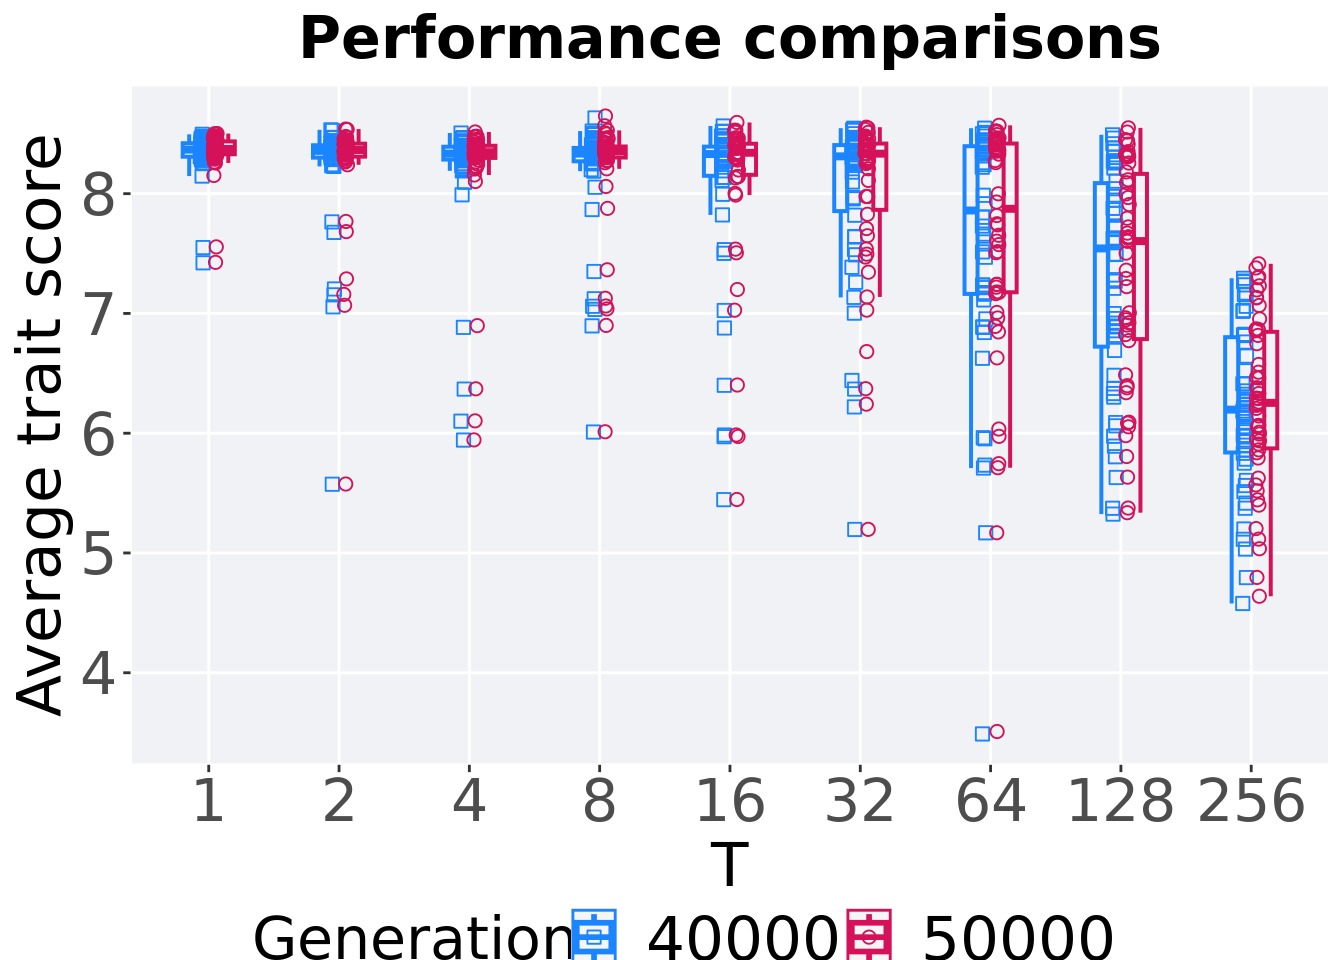
\includegraphics{demo_files/figure-latex/tru-ord-mvc-per-sli-1.pdf}

\hypertarget{stats-25}{%
\subsubsection{Stats}\label{stats-25}}

Summary statistics for the performance of the best performance at 40,000 and 50,000 generations.

\begin{Shaded}
\begin{Highlighting}[]
\NormalTok{slices =}\StringTok{ }\KeywordTok{filter}\NormalTok{(tru_ot_mvc, diagnostic }\OperatorTok{==}\StringTok{ 'ordered_exploitation'} \OperatorTok{&}\StringTok{ }\NormalTok{(gen }\OperatorTok{==}\StringTok{ }\DecValTok{50000} \OperatorTok{|}\StringTok{ }\NormalTok{gen }\OperatorTok{==}\StringTok{ }\DecValTok{40000}\NormalTok{))}
\NormalTok{slices}\OperatorTok{$}\NormalTok{Generation <-}\StringTok{ }\KeywordTok{factor}\NormalTok{(slices}\OperatorTok{$}\NormalTok{gen, }\DataTypeTok{levels =} \KeywordTok{c}\NormalTok{(}\DecValTok{50000}\NormalTok{,}\DecValTok{40000}\NormalTok{))}
\NormalTok{slices }\OperatorTok
\StringTok{  }\KeywordTok{group_by}\NormalTok{(T, Generation) }\OperatorTok
\StringTok{  }\NormalTok{dplyr}\OperatorTok{::}\KeywordTok{summarise}\NormalTok{(}
    \DataTypeTok{count =} \KeywordTok{n}\NormalTok{(),}
    \DataTypeTok{na_cnt =} \KeywordTok{sum}\NormalTok{(}\KeywordTok{is.na}\NormalTok{(pop_fit_max  }\OperatorTok{/}\StringTok{ }\NormalTok{DIMENSIONALITY)),}
    \DataTypeTok{min =} \KeywordTok{min}\NormalTok{(pop_fit_max  }\OperatorTok{/}\StringTok{ }\NormalTok{DIMENSIONALITY, }\DataTypeTok{na.rm =} \OtherTok{TRUE}\NormalTok{),}
    \DataTypeTok{median =} \KeywordTok{median}\NormalTok{(pop_fit_max  }\OperatorTok{/}\StringTok{ }\NormalTok{DIMENSIONALITY, }\DataTypeTok{na.rm =} \OtherTok{TRUE}\NormalTok{),}
    \DataTypeTok{mean =} \KeywordTok{mean}\NormalTok{(pop_fit_max  }\OperatorTok{/}\StringTok{ }\NormalTok{DIMENSIONALITY, }\DataTypeTok{na.rm =} \OtherTok{TRUE}\NormalTok{),}
    \DataTypeTok{max =} \KeywordTok{max}\NormalTok{(pop_fit_max  }\OperatorTok{/}\StringTok{ }\NormalTok{DIMENSIONALITY, }\DataTypeTok{na.rm =} \OtherTok{TRUE}\NormalTok{),}
    \DataTypeTok{IQR =} \KeywordTok{IQR}\NormalTok{(pop_fit_max  }\OperatorTok{/}\StringTok{ }\NormalTok{DIMENSIONALITY, }\DataTypeTok{na.rm =} \OtherTok{TRUE}\NormalTok{)}
\NormalTok{  )}
\end{Highlighting}
\end{Shaded}

\begin{verbatim}
## `summarise()` has grouped output by 'T'. You can override using the `.groups`
## argument.
\end{verbatim}

\begin{verbatim}
## # A tibble: 18 x 9
## # Groups:   T [9]
##    T     Generation count na_cnt   min median  mean   max    IQR
##    <fct> <fct>      <int>  <int> <dbl>  <dbl> <dbl> <dbl>  <dbl>
##  1 1     50000         50      0  7.43   8.37  8.34  8.50 0.108 
##  2 1     40000         50      0  7.42   8.37  8.33  8.50 0.113 
##  3 2     50000         50      0  5.58   8.36  8.23  8.54 0.108 
##  4 2     40000         50      0  5.57   8.36  8.21  8.53 0.104 
##  5 4     50000         50      0  5.94   8.35  8.19  8.52 0.102 
##  6 4     40000         50      0  5.94   8.33  8.18  8.51 0.107 
##  7 8     50000         50      0  6.01   8.35  8.19  8.65 0.0922
##  8 8     40000         50      0  6.01   8.33  8.17  8.63 0.112 
##  9 16    50000         50      0  5.45   8.34  8.08  8.59 0.260 
## 10 16    40000         50      0  5.45   8.33  8.05  8.56 0.244 
## 11 32    50000         50      0  5.20   8.33  8.02  8.56 0.553 
## 12 32    40000         50      0  5.20   8.31  8.00  8.55 0.551 
## 13 64    50000         50      0  3.51   7.87  7.61  8.57 1.24  
## 14 64    40000         50      0  3.49   7.86  7.58  8.55 1.23  
## 15 128   50000         50      0  5.34   7.60  7.33  8.55 1.38  
## 16 128   40000         50      0  5.32   7.54  7.29  8.49 1.37  
## 17 256   50000         50      0  4.64   6.25  6.26  7.41 0.973 
## 18 256   40000         50      0  4.58   6.20  6.21  7.29 0.963
\end{verbatim}

T 2

\begin{Shaded}
\begin{Highlighting}[]
\KeywordTok{wilcox.test}\NormalTok{(}\DataTypeTok{x =} \KeywordTok{filter}\NormalTok{(slices, T }\OperatorTok{==}\StringTok{ }\DecValTok{2} \OperatorTok{&}\StringTok{ }\NormalTok{Generation }\OperatorTok{==}\StringTok{ }\DecValTok{50000}\NormalTok{)}\OperatorTok{$}\NormalTok{pop_fit_max,}
            \DataTypeTok{y =} \KeywordTok{filter}\NormalTok{(slices, T }\OperatorTok{==}\StringTok{ }\DecValTok{2} \OperatorTok{&}\StringTok{ }\NormalTok{Generation }\OperatorTok{==}\StringTok{ }\DecValTok{40000}\NormalTok{)}\OperatorTok{$}\NormalTok{pop_fit_max,}
            \DataTypeTok{alternative =} \StringTok{'t'}\NormalTok{)}
\end{Highlighting}
\end{Shaded}

\begin{verbatim}
## 
##  Wilcoxon rank sum test with continuity correction
## 
## data:  filter(slices, T == 2 & Generation == 50000)$pop_fit_max and filter(slices, T == 2 & Generation == 40000)$pop_fit_max
## W = 1359, p-value = 0.4545
## alternative hypothesis: true location shift is not equal to 0
\end{verbatim}

T 4

\begin{Shaded}
\begin{Highlighting}[]
\KeywordTok{wilcox.test}\NormalTok{(}\DataTypeTok{x =} \KeywordTok{filter}\NormalTok{(slices, T }\OperatorTok{==}\StringTok{ }\DecValTok{4} \OperatorTok{&}\StringTok{ }\NormalTok{Generation }\OperatorTok{==}\StringTok{ }\DecValTok{50000}\NormalTok{)}\OperatorTok{$}\NormalTok{pop_fit_max,}
            \DataTypeTok{y =} \KeywordTok{filter}\NormalTok{(slices, T }\OperatorTok{==}\StringTok{ }\DecValTok{4} \OperatorTok{&}\StringTok{ }\NormalTok{Generation }\OperatorTok{==}\StringTok{ }\DecValTok{40000}\NormalTok{)}\OperatorTok{$}\NormalTok{pop_fit_max,}
            \DataTypeTok{alternative =} \StringTok{'t'}\NormalTok{)}
\end{Highlighting}
\end{Shaded}

\begin{verbatim}
## 
##  Wilcoxon rank sum test with continuity correction
## 
## data:  filter(slices, T == 4 & Generation == 50000)$pop_fit_max and filter(slices, T == 4 & Generation == 40000)$pop_fit_max
## W = 1355, p-value = 0.4713
## alternative hypothesis: true location shift is not equal to 0
\end{verbatim}

T 8

\begin{Shaded}
\begin{Highlighting}[]
\KeywordTok{wilcox.test}\NormalTok{(}\DataTypeTok{x =} \KeywordTok{filter}\NormalTok{(slices, T }\OperatorTok{==}\StringTok{ }\DecValTok{8} \OperatorTok{&}\StringTok{ }\NormalTok{Generation }\OperatorTok{==}\StringTok{ }\DecValTok{50000}\NormalTok{)}\OperatorTok{$}\NormalTok{pop_fit_max,}
            \DataTypeTok{y =} \KeywordTok{filter}\NormalTok{(slices, T }\OperatorTok{==}\StringTok{ }\DecValTok{8} \OperatorTok{&}\StringTok{ }\NormalTok{Generation }\OperatorTok{==}\StringTok{ }\DecValTok{40000}\NormalTok{)}\OperatorTok{$}\NormalTok{pop_fit_max,}
            \DataTypeTok{alternative =} \StringTok{'t'}\NormalTok{)}
\end{Highlighting}
\end{Shaded}

\begin{verbatim}
## 
##  Wilcoxon rank sum test with continuity correction
## 
## data:  filter(slices, T == 8 & Generation == 50000)$pop_fit_max and filter(slices, T == 8 & Generation == 40000)$pop_fit_max
## W = 1375, p-value = 0.3907
## alternative hypothesis: true location shift is not equal to 0
\end{verbatim}

T 16

\begin{Shaded}
\begin{Highlighting}[]
\KeywordTok{wilcox.test}\NormalTok{(}\DataTypeTok{x =} \KeywordTok{filter}\NormalTok{(slices, T }\OperatorTok{==}\StringTok{ }\DecValTok{16} \OperatorTok{&}\StringTok{ }\NormalTok{Generation }\OperatorTok{==}\StringTok{ }\DecValTok{50000}\NormalTok{)}\OperatorTok{$}\NormalTok{pop_fit_max,}
            \DataTypeTok{y =} \KeywordTok{filter}\NormalTok{(slices, T }\OperatorTok{==}\StringTok{ }\DecValTok{16} \OperatorTok{&}\StringTok{ }\NormalTok{Generation }\OperatorTok{==}\StringTok{ }\DecValTok{40000}\NormalTok{)}\OperatorTok{$}\NormalTok{pop_fit_max,}
            \DataTypeTok{alternative =} \StringTok{'t'}\NormalTok{)}
\end{Highlighting}
\end{Shaded}

\begin{verbatim}
## 
##  Wilcoxon rank sum test with continuity correction
## 
## data:  filter(slices, T == 16 & Generation == 50000)$pop_fit_max and filter(slices, T == 16 & Generation == 40000)$pop_fit_max
## W = 1367, p-value = 0.4219
## alternative hypothesis: true location shift is not equal to 0
\end{verbatim}

T 32

\begin{Shaded}
\begin{Highlighting}[]
\KeywordTok{wilcox.test}\NormalTok{(}\DataTypeTok{x =} \KeywordTok{filter}\NormalTok{(slices, T }\OperatorTok{==}\StringTok{ }\DecValTok{32} \OperatorTok{&}\StringTok{ }\NormalTok{Generation }\OperatorTok{==}\StringTok{ }\DecValTok{50000}\NormalTok{)}\OperatorTok{$}\NormalTok{pop_fit_max,}
            \DataTypeTok{y =} \KeywordTok{filter}\NormalTok{(slices, T }\OperatorTok{==}\StringTok{ }\DecValTok{32} \OperatorTok{&}\StringTok{ }\NormalTok{Generation }\OperatorTok{==}\StringTok{ }\DecValTok{40000}\NormalTok{)}\OperatorTok{$}\NormalTok{pop_fit_max,}
            \DataTypeTok{alternative =} \StringTok{'t'}\NormalTok{)}
\end{Highlighting}
\end{Shaded}

\begin{verbatim}
## 
##  Wilcoxon rank sum test with continuity correction
## 
## data:  filter(slices, T == 32 & Generation == 50000)$pop_fit_max and filter(slices, T == 32 & Generation == 40000)$pop_fit_max
## W = 1320, p-value = 0.6319
## alternative hypothesis: true location shift is not equal to 0
\end{verbatim}

T 64

\begin{Shaded}
\begin{Highlighting}[]
\KeywordTok{wilcox.test}\NormalTok{(}\DataTypeTok{x =} \KeywordTok{filter}\NormalTok{(slices, T }\OperatorTok{==}\StringTok{ }\DecValTok{64} \OperatorTok{&}\StringTok{ }\NormalTok{Generation }\OperatorTok{==}\StringTok{ }\DecValTok{50000}\NormalTok{)}\OperatorTok{$}\NormalTok{pop_fit_max,}
            \DataTypeTok{y =} \KeywordTok{filter}\NormalTok{(slices, T }\OperatorTok{==}\StringTok{ }\DecValTok{64} \OperatorTok{&}\StringTok{ }\NormalTok{Generation }\OperatorTok{==}\StringTok{ }\DecValTok{40000}\NormalTok{)}\OperatorTok{$}\NormalTok{pop_fit_max,}
            \DataTypeTok{alternative =} \StringTok{'t'}\NormalTok{)}
\end{Highlighting}
\end{Shaded}

\begin{verbatim}
## 
##  Wilcoxon rank sum test with continuity correction
## 
## data:  filter(slices, T == 64 & Generation == 50000)$pop_fit_max and filter(slices, T == 64 & Generation == 40000)$pop_fit_max
## W = 1319, p-value = 0.6368
## alternative hypothesis: true location shift is not equal to 0
\end{verbatim}

T 128

\begin{Shaded}
\begin{Highlighting}[]
\KeywordTok{wilcox.test}\NormalTok{(}\DataTypeTok{x =} \KeywordTok{filter}\NormalTok{(slices, T }\OperatorTok{==}\StringTok{ }\DecValTok{128} \OperatorTok{&}\StringTok{ }\NormalTok{Generation }\OperatorTok{==}\StringTok{ }\DecValTok{50000}\NormalTok{)}\OperatorTok{$}\NormalTok{pop_fit_max,}
            \DataTypeTok{y =} \KeywordTok{filter}\NormalTok{(slices, T }\OperatorTok{==}\StringTok{ }\DecValTok{128} \OperatorTok{&}\StringTok{ }\NormalTok{Generation }\OperatorTok{==}\StringTok{ }\DecValTok{40000}\NormalTok{)}\OperatorTok{$}\NormalTok{pop_fit_max,}
            \DataTypeTok{alternative =} \StringTok{'t'}\NormalTok{)}
\end{Highlighting}
\end{Shaded}

\begin{verbatim}
## 
##  Wilcoxon rank sum test with continuity correction
## 
## data:  filter(slices, T == 128 & Generation == 50000)$pop_fit_max and filter(slices, T == 128 & Generation == 40000)$pop_fit_max
## W = 1311, p-value = 0.6766
## alternative hypothesis: true location shift is not equal to 0
\end{verbatim}

T 256

\begin{Shaded}
\begin{Highlighting}[]
\KeywordTok{wilcox.test}\NormalTok{(}\DataTypeTok{x =} \KeywordTok{filter}\NormalTok{(slices, T }\OperatorTok{==}\StringTok{ }\DecValTok{256} \OperatorTok{&}\StringTok{ }\NormalTok{Generation }\OperatorTok{==}\StringTok{ }\DecValTok{50000}\NormalTok{)}\OperatorTok{$}\NormalTok{pop_fit_max,}
            \DataTypeTok{y =} \KeywordTok{filter}\NormalTok{(slices, T }\OperatorTok{==}\StringTok{ }\DecValTok{256} \OperatorTok{&}\StringTok{ }\NormalTok{Generation }\OperatorTok{==}\StringTok{ }\DecValTok{40000}\NormalTok{)}\OperatorTok{$}\NormalTok{pop_fit_max,}
            \DataTypeTok{alternative =} \StringTok{'t'}\NormalTok{)}
\end{Highlighting}
\end{Shaded}

\begin{verbatim}
## 
##  Wilcoxon rank sum test with continuity correction
## 
## data:  filter(slices, T == 256 & Generation == 50000)$pop_fit_max and filter(slices, T == 256 & Generation == 40000)$pop_fit_max
## W = 1321, p-value = 0.627
## alternative hypothesis: true location shift is not equal to 0
\end{verbatim}

\hypertarget{contraditory-objectives-diagnostic}{%
\section{Contraditory objectives diagnostic}\label{contraditory-objectives-diagnostic}}

Here we present the results for \textbf{satisfactory trait coverage} and \textbf{activation gene coverage} found by each truncation selection size value replicate on the ordered exploitation diagnostic.
Satisfactory trait coverage refers to the count of unique satisfied traits in the population, while activation gene coverage refers to the count of unique activation genes in the population.
Note that both coverage values fall between 0 and 100.

\hypertarget{satisfactory-trait-coverage-2}{%
\subsection{Satisfactory trait coverage}\label{satisfactory-trait-coverage-2}}

Satisfactory trait coverage analysis.

\hypertarget{coverage-over-time-5}{%
\subsubsection{Coverage over time}\label{coverage-over-time-5}}

Satisfactory trait coverage over time.

\begin{Shaded}
\begin{Highlighting}[]
\NormalTok{lines =}\StringTok{ }\KeywordTok{filter}\NormalTok{(tru_ot, diagnostic }\OperatorTok{==}\StringTok{ 'contradictory_objectives'}\NormalTok{) }\OperatorTok
\StringTok{        }\KeywordTok{group_by}\NormalTok{(T, gen) }\OperatorTok
\StringTok{          }\NormalTok{dplyr}\OperatorTok{::}\KeywordTok{summarise}\NormalTok{(}
            \DataTypeTok{min =} \KeywordTok{min}\NormalTok{(pop_uni_obj),}
            \DataTypeTok{mean =} \KeywordTok{mean}\NormalTok{(pop_uni_obj),}
            \DataTypeTok{max =} \KeywordTok{max}\NormalTok{(pop_uni_obj)}
\NormalTok{          )}
\end{Highlighting}
\end{Shaded}

\begin{verbatim}
## `summarise()` has grouped output by 'T'. You can override using the `.groups`
## argument.
\end{verbatim}

\begin{Shaded}
\begin{Highlighting}[]
\KeywordTok{ggplot}\NormalTok{(lines, }\KeywordTok{aes}\NormalTok{(}\DataTypeTok{x=}\NormalTok{gen, }\DataTypeTok{y=}\NormalTok{mean, }\DataTypeTok{group =}\NormalTok{ T, }\DataTypeTok{fill =}\NormalTok{T, }\DataTypeTok{color =}\NormalTok{ T, }\DataTypeTok{shape =}\NormalTok{ T)) }\OperatorTok{+}
\StringTok{  }\KeywordTok{geom_ribbon}\NormalTok{(}\KeywordTok{aes}\NormalTok{(}\DataTypeTok{ymin =}\NormalTok{ min, }\DataTypeTok{ymax =}\NormalTok{ max), }\DataTypeTok{alpha =} \FloatTok{0.1}\NormalTok{) }\OperatorTok{+}
\StringTok{  }\KeywordTok{geom_line}\NormalTok{(}\DataTypeTok{size =} \FloatTok{0.5}\NormalTok{) }\OperatorTok{+}
\StringTok{  }\KeywordTok{geom_point}\NormalTok{(}\DataTypeTok{data =} \KeywordTok{filter}\NormalTok{(lines, gen }\OperatorTok\StringTok{ }\DecValTok{2000} \OperatorTok{==}\StringTok{ }\DecValTok{0} \OperatorTok{&}\StringTok{ }\NormalTok{gen }\OperatorTok{!=}\StringTok{ }\DecValTok{0}\NormalTok{), }\DataTypeTok{size =} \FloatTok{1.5}\NormalTok{, }\DataTypeTok{stroke =} \FloatTok{2.0}\NormalTok{, }\DataTypeTok{alpha =} \FloatTok{1.0}\NormalTok{) }\OperatorTok{+}
\StringTok{  }\KeywordTok{scale_y_continuous}\NormalTok{(}
    \DataTypeTok{name=}\StringTok{"Coverage"}
\NormalTok{  ) }\OperatorTok{+}
\StringTok{  }\KeywordTok{scale_x_continuous}\NormalTok{(}
    \DataTypeTok{name=}\StringTok{"Generations"}\NormalTok{,}
    \DataTypeTok{limits=}\KeywordTok{c}\NormalTok{(}\DecValTok{0}\NormalTok{, }\DecValTok{50000}\NormalTok{),}
    \DataTypeTok{breaks=}\KeywordTok{c}\NormalTok{(}\DecValTok{0}\NormalTok{, }\DecValTok{10000}\NormalTok{, }\DecValTok{20000}\NormalTok{, }\DecValTok{30000}\NormalTok{, }\DecValTok{40000}\NormalTok{, }\DecValTok{50000}\NormalTok{),}
    \DataTypeTok{labels=}\KeywordTok{c}\NormalTok{(}\StringTok{"0e+4"}\NormalTok{, }\StringTok{"1e+4"}\NormalTok{, }\StringTok{"2e+4"}\NormalTok{, }\StringTok{"3e+4"}\NormalTok{, }\StringTok{"4e+4"}\NormalTok{, }\StringTok{"5e+4"}\NormalTok{)}

\NormalTok{  ) }\OperatorTok{+}
\StringTok{  }\KeywordTok{scale_shape_manual}\NormalTok{(}\DataTypeTok{values=}\NormalTok{SHAPE)}\OperatorTok{+}
\StringTok{  }\KeywordTok{scale_colour_manual}\NormalTok{(}\DataTypeTok{values =}\NormalTok{ cb_palette) }\OperatorTok{+}
\StringTok{  }\KeywordTok{scale_fill_manual}\NormalTok{(}\DataTypeTok{values =}\NormalTok{ cb_palette) }\OperatorTok{+}
\StringTok{  }\KeywordTok{ggtitle}\NormalTok{(}\StringTok{"Satisfactory trait coverage over time"}\NormalTok{) }\OperatorTok{+}
\StringTok{  }\NormalTok{p_theme}
\end{Highlighting}
\end{Shaded}

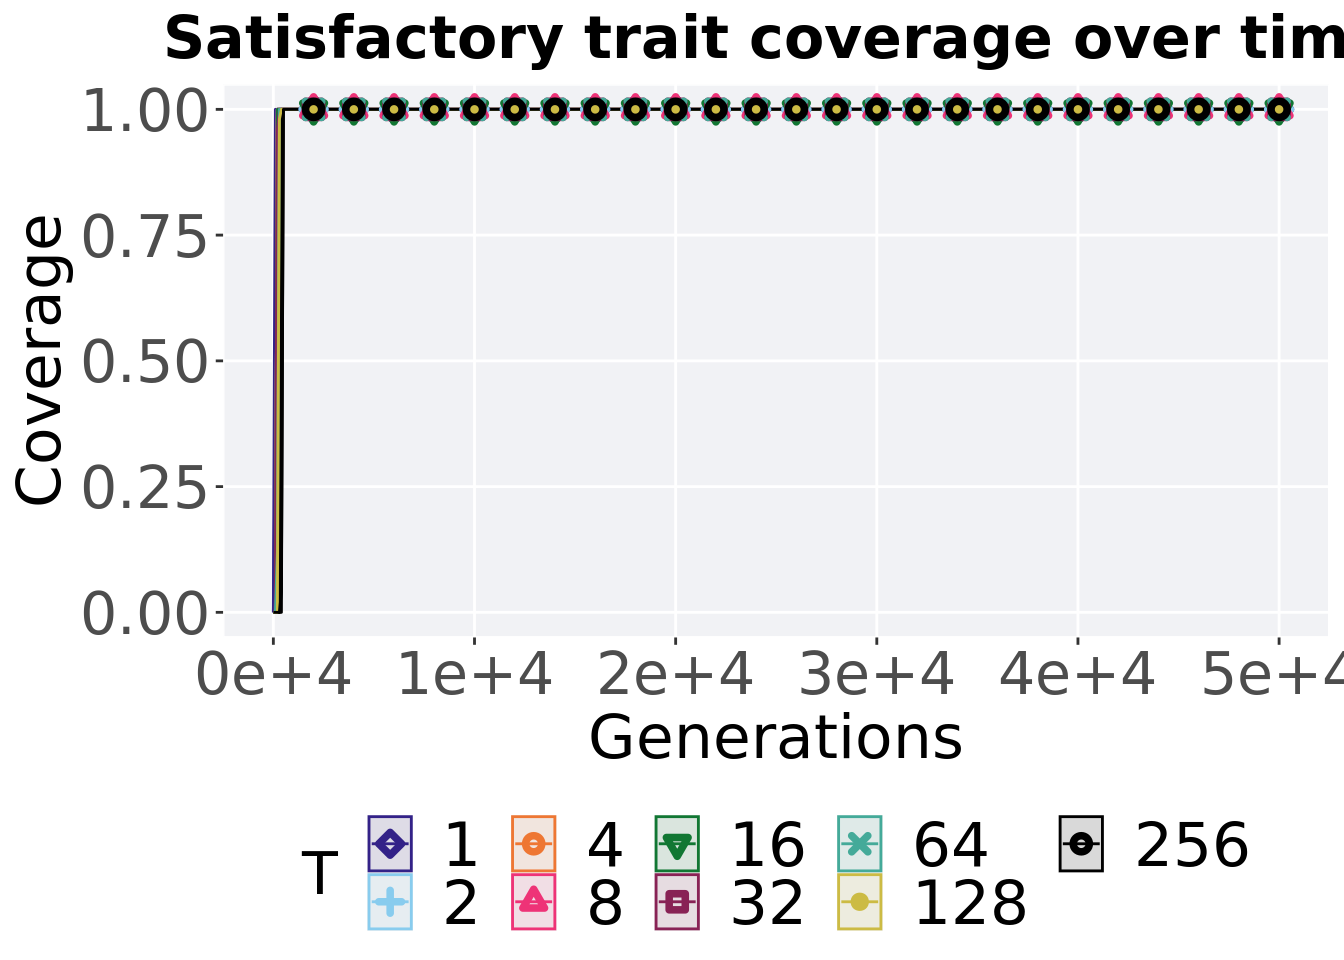
\includegraphics{demo_files/figure-latex/tru-con-sat-1.pdf}

\hypertarget{best-coverage-throughout-3}{%
\subsubsection{Best coverage throughout}\label{best-coverage-throughout-3}}

Best satisfactory trait coverage throughout 50,000 generations.

\begin{Shaded}
\begin{Highlighting}[]
\KeywordTok{filter}\NormalTok{(tru_best, col }\OperatorTok{==}\StringTok{ 'pop_uni_obj'} \OperatorTok{&}\StringTok{ }\NormalTok{diagnostic }\OperatorTok{==}\StringTok{ 'contradictory_objectives'}\NormalTok{) }\OperatorTok
\KeywordTok{ggplot}\NormalTok{(., }\KeywordTok{aes}\NormalTok{(}\DataTypeTok{x =}\NormalTok{ T, }\DataTypeTok{y =}\NormalTok{ val, }\DataTypeTok{color =}\NormalTok{ T, }\DataTypeTok{fill =}\NormalTok{ T, }\DataTypeTok{shape =}\NormalTok{ T)) }\OperatorTok{+}
\StringTok{  }\KeywordTok{geom_flat_violin}\NormalTok{(}\DataTypeTok{position =} \KeywordTok{position_nudge}\NormalTok{(}\DataTypeTok{x =} \FloatTok{.2}\NormalTok{, }\DataTypeTok{y =} \DecValTok{0}\NormalTok{), }\DataTypeTok{scale =} \StringTok{'width'}\NormalTok{, }\DataTypeTok{alpha =} \FloatTok{0.2}\NormalTok{) }\OperatorTok{+}
\StringTok{  }\KeywordTok{geom_point}\NormalTok{(}\DataTypeTok{position =} \KeywordTok{position_jitter}\NormalTok{(}\DataTypeTok{width =} \FloatTok{.1}\NormalTok{), }\DataTypeTok{size =} \FloatTok{1.5}\NormalTok{, }\DataTypeTok{alpha =} \FloatTok{1.0}\NormalTok{) }\OperatorTok{+}
\StringTok{  }\KeywordTok{geom_boxplot}\NormalTok{(}\DataTypeTok{color =} \StringTok{'black'}\NormalTok{, }\DataTypeTok{width =} \FloatTok{.2}\NormalTok{, }\DataTypeTok{outlier.shape =} \OtherTok{NA}\NormalTok{, }\DataTypeTok{alpha =} \FloatTok{0.0}\NormalTok{) }\OperatorTok{+}
\StringTok{  }\KeywordTok{scale_y_continuous}\NormalTok{(}
    \DataTypeTok{name=}\StringTok{"Coverage"}
\NormalTok{  ) }\OperatorTok{+}
\StringTok{  }\KeywordTok{scale_x_discrete}\NormalTok{(}
    \DataTypeTok{name=}\StringTok{"T"}
\NormalTok{  )}\OperatorTok{+}
\StringTok{  }\KeywordTok{scale_shape_manual}\NormalTok{(}\DataTypeTok{values=}\NormalTok{SHAPE)}\OperatorTok{+}
\StringTok{  }\KeywordTok{scale_colour_manual}\NormalTok{(}\DataTypeTok{values =}\NormalTok{ cb_palette) }\OperatorTok{+}
\StringTok{  }\KeywordTok{scale_fill_manual}\NormalTok{(}\DataTypeTok{values =}\NormalTok{ cb_palette) }\OperatorTok{+}
\StringTok{  }\KeywordTok{ggtitle}\NormalTok{(}\StringTok{"Best satisfactory trait coverage"}\NormalTok{) }\OperatorTok{+}
\StringTok{  }\NormalTok{p_theme}
\end{Highlighting}
\end{Shaded}

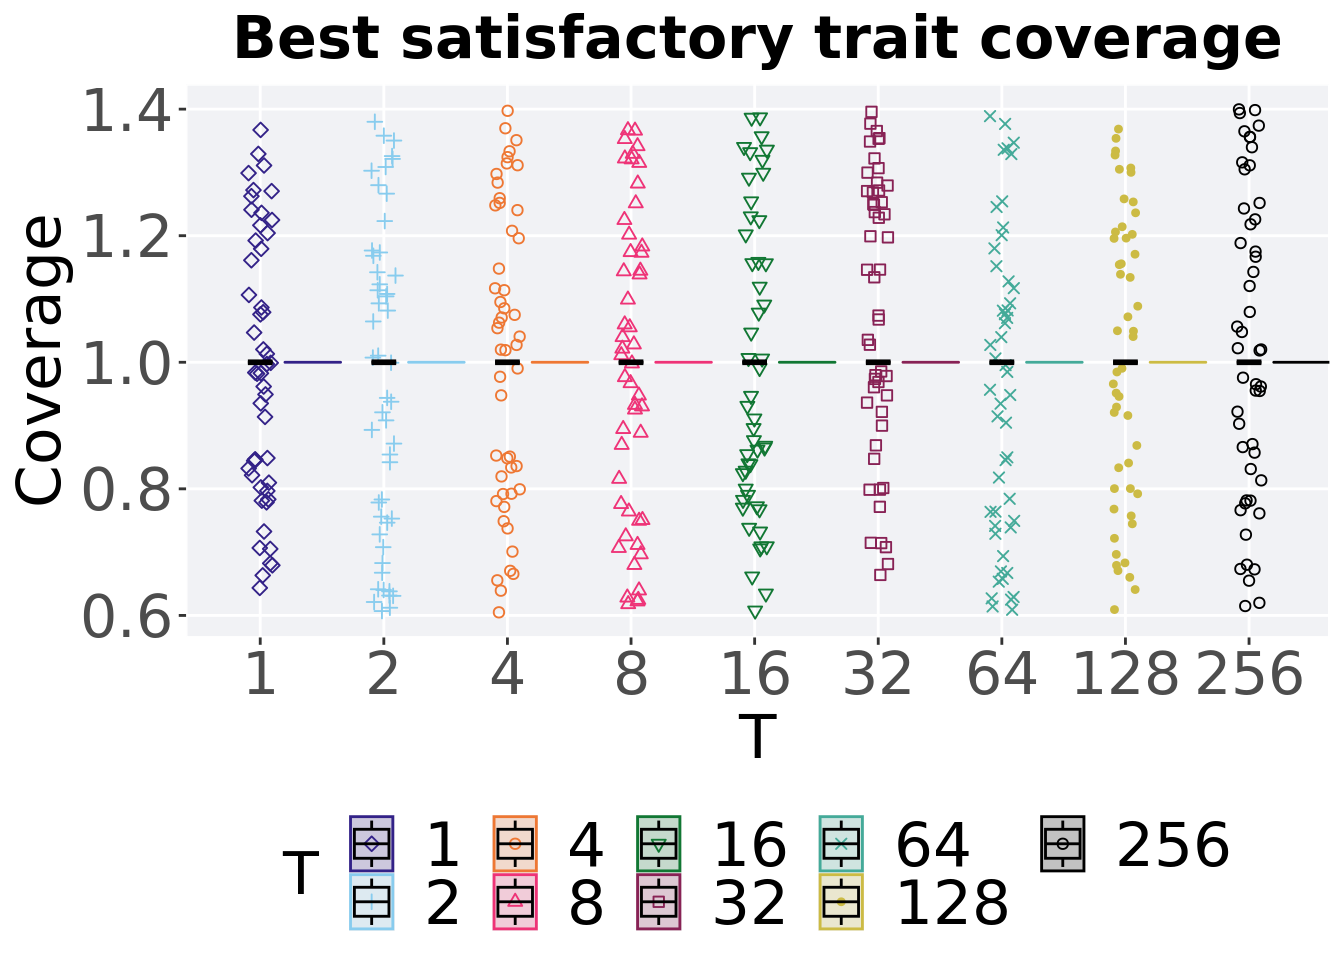
\includegraphics{demo_files/figure-latex/tru-con-sat-bst-1.pdf}

\hypertarget{stats-26}{%
\paragraph{Stats}\label{stats-26}}

Summary statistics for the best satisfactory trait coverage throughout 50,000 generations.

\begin{Shaded}
\begin{Highlighting}[]
\NormalTok{coverage =}\StringTok{ }\KeywordTok{filter}\NormalTok{(tru_best, col }\OperatorTok{==}\StringTok{ 'pop_uni_obj'} \OperatorTok{&}\StringTok{ }\NormalTok{diagnostic }\OperatorTok{==}\StringTok{ 'contradictory_objectives'}\NormalTok{)}
\KeywordTok{group_by}\NormalTok{(coverage, T) }\OperatorTok
\StringTok{  }\NormalTok{dplyr}\OperatorTok{::}\KeywordTok{summarise}\NormalTok{(}
    \DataTypeTok{count =} \KeywordTok{n}\NormalTok{(),}
    \DataTypeTok{na_cnt =} \KeywordTok{sum}\NormalTok{(}\KeywordTok{is.na}\NormalTok{(val)),}
    \DataTypeTok{min =} \KeywordTok{min}\NormalTok{(val, }\DataTypeTok{na.rm =} \OtherTok{TRUE}\NormalTok{),}
    \DataTypeTok{median =} \KeywordTok{median}\NormalTok{(val, }\DataTypeTok{na.rm =} \OtherTok{TRUE}\NormalTok{),}
    \DataTypeTok{mean =} \KeywordTok{mean}\NormalTok{(val, }\DataTypeTok{na.rm =} \OtherTok{TRUE}\NormalTok{),}
    \DataTypeTok{max =} \KeywordTok{max}\NormalTok{(val, }\DataTypeTok{na.rm =} \OtherTok{TRUE}\NormalTok{),}
    \DataTypeTok{IQR =} \KeywordTok{IQR}\NormalTok{(val, }\DataTypeTok{na.rm =} \OtherTok{TRUE}\NormalTok{)}
\NormalTok{  )}
\end{Highlighting}
\end{Shaded}

\begin{verbatim}
## # A tibble: 9 x 8
##   T     count na_cnt   min median  mean   max   IQR
##   <fct> <int>  <int> <dbl>  <dbl> <dbl> <dbl> <dbl>
## 1 1        50      0     1      1     1     1     0
## 2 2        50      0     1      1     1     1     0
## 3 4        50      0     1      1     1     1     0
## 4 8        50      0     1      1     1     1     0
## 5 16       50      0     1      1     1     1     0
## 6 32       50      0     1      1     1     1     0
## 7 64       50      0     1      1     1     1     0
## 8 128      50      0     1      1     1     1     0
## 9 256      50      0     1      1     1     1     0
\end{verbatim}

\hypertarget{end-of-50000-generations-5}{%
\subsubsection{End of 50,000 generations}\label{end-of-50000-generations-5}}

Satisfactory trait coverage in the population at the end of 50,000 generations.

\begin{Shaded}
\begin{Highlighting}[]
\KeywordTok{filter}\NormalTok{(tru_ot, diagnostic }\OperatorTok{==}\StringTok{ 'contradictory_objectives'} \OperatorTok{&}\StringTok{ }\NormalTok{gen }\OperatorTok{==}\StringTok{ }\DecValTok{50000}\NormalTok{) }\OperatorTok
\KeywordTok{ggplot}\NormalTok{(., }\KeywordTok{aes}\NormalTok{(}\DataTypeTok{x =}\NormalTok{ T, }\DataTypeTok{y =}\NormalTok{ pop_uni_obj, }\DataTypeTok{color =}\NormalTok{ T, }\DataTypeTok{fill =}\NormalTok{ T, }\DataTypeTok{shape =}\NormalTok{ T)) }\OperatorTok{+}
\StringTok{  }\KeywordTok{geom_flat_violin}\NormalTok{(}\DataTypeTok{position =} \KeywordTok{position_nudge}\NormalTok{(}\DataTypeTok{x =} \FloatTok{.2}\NormalTok{, }\DataTypeTok{y =} \DecValTok{0}\NormalTok{), }\DataTypeTok{scale =} \StringTok{'width'}\NormalTok{, }\DataTypeTok{alpha =} \FloatTok{0.2}\NormalTok{) }\OperatorTok{+}
\StringTok{  }\KeywordTok{geom_point}\NormalTok{(}\DataTypeTok{position =} \KeywordTok{position_jitter}\NormalTok{(}\DataTypeTok{width =} \FloatTok{.1}\NormalTok{), }\DataTypeTok{size =} \FloatTok{1.5}\NormalTok{, }\DataTypeTok{alpha =} \FloatTok{1.0}\NormalTok{) }\OperatorTok{+}
\StringTok{  }\KeywordTok{geom_boxplot}\NormalTok{(}\DataTypeTok{color =} \StringTok{'black'}\NormalTok{, }\DataTypeTok{width =} \FloatTok{.2}\NormalTok{, }\DataTypeTok{outlier.shape =} \OtherTok{NA}\NormalTok{, }\DataTypeTok{alpha =} \FloatTok{0.0}\NormalTok{) }\OperatorTok{+}
\StringTok{  }\KeywordTok{scale_y_continuous}\NormalTok{(}
    \DataTypeTok{name=}\StringTok{"Coverage"}
\NormalTok{  ) }\OperatorTok{+}
\StringTok{  }\KeywordTok{scale_x_discrete}\NormalTok{(}
    \DataTypeTok{name=}\StringTok{"T"}
\NormalTok{  )}\OperatorTok{+}
\StringTok{  }\KeywordTok{scale_shape_manual}\NormalTok{(}\DataTypeTok{values=}\NormalTok{SHAPE)}\OperatorTok{+}
\StringTok{  }\KeywordTok{scale_colour_manual}\NormalTok{(}\DataTypeTok{values =}\NormalTok{ cb_palette) }\OperatorTok{+}
\StringTok{  }\KeywordTok{scale_fill_manual}\NormalTok{(}\DataTypeTok{values =}\NormalTok{ cb_palette) }\OperatorTok{+}
\StringTok{  }\KeywordTok{ggtitle}\NormalTok{(}\StringTok{"Final satisfactory trait coverage"}\NormalTok{) }\OperatorTok{+}
\StringTok{  }\NormalTok{p_theme}
\end{Highlighting}
\end{Shaded}

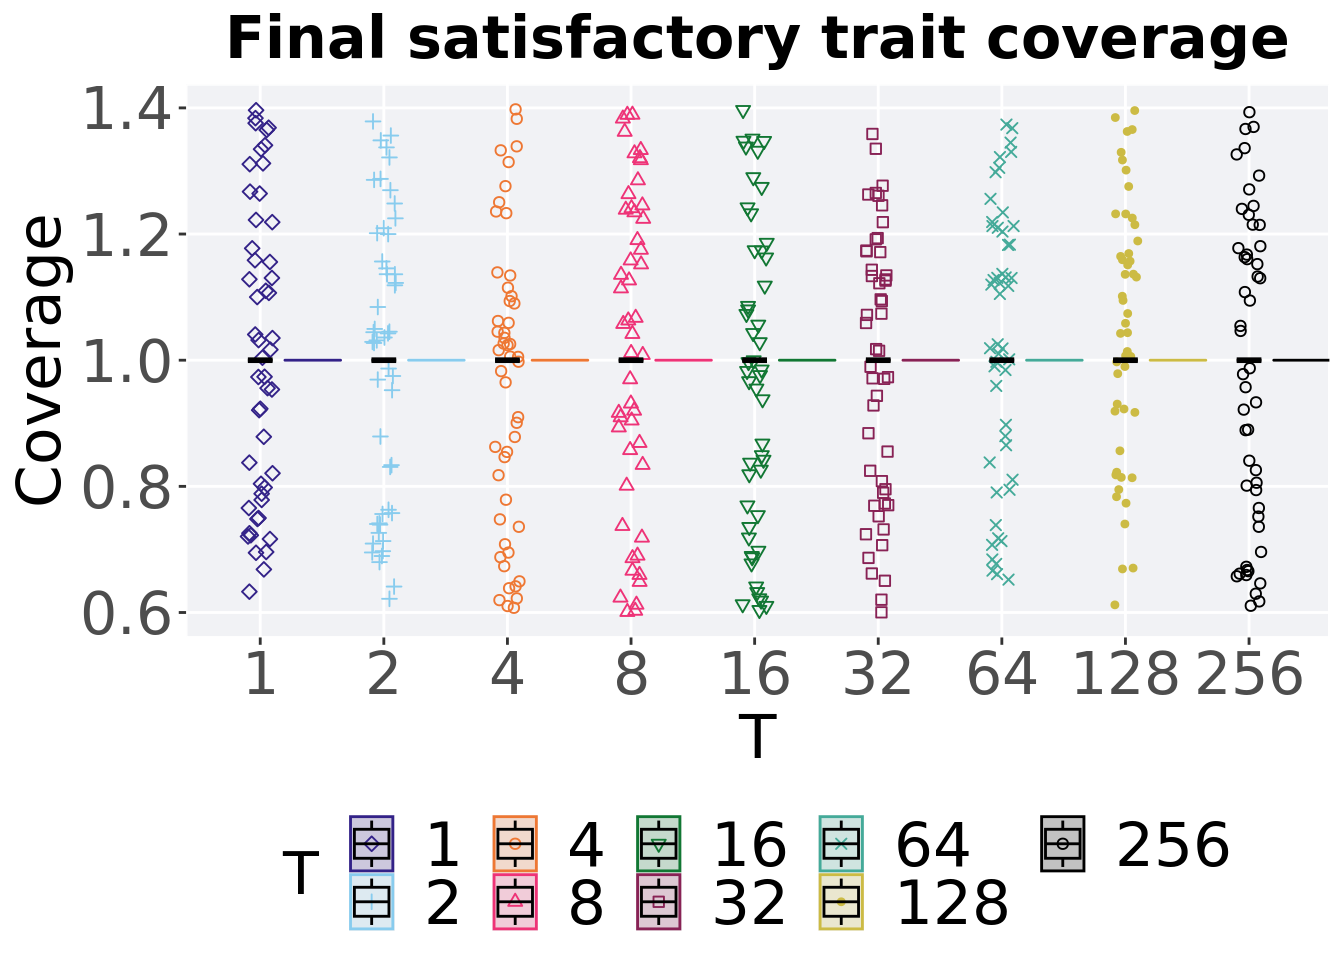
\includegraphics{demo_files/figure-latex/tru-con-sat-end-1.pdf}

\hypertarget{stats-27}{%
\paragraph{Stats}\label{stats-27}}

Summary statistics for satisfactory trait coverage in the population at the end of 50,000 generations.

\begin{Shaded}
\begin{Highlighting}[]
\NormalTok{coverage =}\StringTok{ }\KeywordTok{filter}\NormalTok{(tru_ot, diagnostic }\OperatorTok{==}\StringTok{ 'contradictory_objectives'} \OperatorTok{&}\StringTok{ }\NormalTok{gen }\OperatorTok{==}\StringTok{ }\DecValTok{50000}\NormalTok{)}
\KeywordTok{group_by}\NormalTok{(coverage, T) }\OperatorTok
\StringTok{  }\NormalTok{dplyr}\OperatorTok{::}\KeywordTok{summarise}\NormalTok{(}
    \DataTypeTok{count =} \KeywordTok{n}\NormalTok{(),}
    \DataTypeTok{na_cnt =} \KeywordTok{sum}\NormalTok{(}\KeywordTok{is.na}\NormalTok{(pop_uni_obj)),}
    \DataTypeTok{min =} \KeywordTok{min}\NormalTok{(pop_uni_obj, }\DataTypeTok{na.rm =} \OtherTok{TRUE}\NormalTok{),}
    \DataTypeTok{median =} \KeywordTok{median}\NormalTok{(pop_uni_obj, }\DataTypeTok{na.rm =} \OtherTok{TRUE}\NormalTok{),}
    \DataTypeTok{mean =} \KeywordTok{mean}\NormalTok{(pop_uni_obj, }\DataTypeTok{na.rm =} \OtherTok{TRUE}\NormalTok{),}
    \DataTypeTok{max =} \KeywordTok{max}\NormalTok{(pop_uni_obj, }\DataTypeTok{na.rm =} \OtherTok{TRUE}\NormalTok{),}
    \DataTypeTok{IQR =} \KeywordTok{IQR}\NormalTok{(pop_uni_obj, }\DataTypeTok{na.rm =} \OtherTok{TRUE}\NormalTok{)}
\NormalTok{  )}
\end{Highlighting}
\end{Shaded}

\begin{verbatim}
## # A tibble: 9 x 8
##   T     count na_cnt   min median  mean   max   IQR
##   <fct> <int>  <int> <int>  <dbl> <dbl> <int> <dbl>
## 1 1        50      0     1      1     1     1     0
## 2 2        50      0     1      1     1     1     0
## 3 4        50      0     1      1     1     1     0
## 4 8        50      0     1      1     1     1     0
## 5 16       50      0     1      1     1     1     0
## 6 32       50      0     1      1     1     1     0
## 7 64       50      0     1      1     1     1     0
## 8 128      50      0     1      1     1     1     0
## 9 256      50      0     1      1     1     1     0
\end{verbatim}

\hypertarget{activation-gene-coverage-4}{%
\subsection{Activation gene coverage}\label{activation-gene-coverage-4}}

Here we analyze the activation gene coverage for each parameter replicate on the contradictory objectives diagnostic.

\hypertarget{coverage-over-time-6}{%
\subsubsection{Coverage over time}\label{coverage-over-time-6}}

Activation gene coverage over time.

\begin{Shaded}
\begin{Highlighting}[]
\NormalTok{lines =}\StringTok{ }\KeywordTok{filter}\NormalTok{(tru_ot, diagnostic }\OperatorTok{==}\StringTok{ 'contradictory_objectives'}\NormalTok{) }\OperatorTok
\StringTok{        }\KeywordTok{group_by}\NormalTok{(T, gen) }\OperatorTok
\StringTok{          }\NormalTok{dplyr}\OperatorTok{::}\KeywordTok{summarise}\NormalTok{(}
            \DataTypeTok{min =} \KeywordTok{min}\NormalTok{(uni_str_pos),}
            \DataTypeTok{mean =} \KeywordTok{mean}\NormalTok{(uni_str_pos),}
            \DataTypeTok{max =} \KeywordTok{max}\NormalTok{(uni_str_pos)}
\NormalTok{          )}
\end{Highlighting}
\end{Shaded}

\begin{verbatim}
## `summarise()` has grouped output by 'T'. You can override using the `.groups`
## argument.
\end{verbatim}

\begin{Shaded}
\begin{Highlighting}[]
\KeywordTok{ggplot}\NormalTok{(lines, }\KeywordTok{aes}\NormalTok{(}\DataTypeTok{x=}\NormalTok{gen, }\DataTypeTok{y=}\NormalTok{mean, }\DataTypeTok{group =}\NormalTok{ T, }\DataTypeTok{fill =}\NormalTok{T, }\DataTypeTok{color =}\NormalTok{ T, }\DataTypeTok{shape =}\NormalTok{ T)) }\OperatorTok{+}
\StringTok{  }\KeywordTok{geom_ribbon}\NormalTok{(}\KeywordTok{aes}\NormalTok{(}\DataTypeTok{ymin =}\NormalTok{ min, }\DataTypeTok{ymax =}\NormalTok{ max), }\DataTypeTok{alpha =} \FloatTok{0.1}\NormalTok{) }\OperatorTok{+}
\StringTok{  }\KeywordTok{geom_line}\NormalTok{(}\DataTypeTok{size =} \FloatTok{0.5}\NormalTok{) }\OperatorTok{+}
\StringTok{  }\KeywordTok{geom_point}\NormalTok{(}\DataTypeTok{data =} \KeywordTok{filter}\NormalTok{(lines, gen }\OperatorTok\StringTok{ }\DecValTok{2000} \OperatorTok{==}\StringTok{ }\DecValTok{0} \OperatorTok{&}\StringTok{ }\NormalTok{gen }\OperatorTok{!=}\StringTok{ }\DecValTok{0}\NormalTok{), }\DataTypeTok{size =} \FloatTok{1.5}\NormalTok{, }\DataTypeTok{stroke =} \FloatTok{2.0}\NormalTok{, }\DataTypeTok{alpha =} \FloatTok{1.0}\NormalTok{) }\OperatorTok{+}
\StringTok{  }\KeywordTok{scale_y_continuous}\NormalTok{(}
    \DataTypeTok{name=}\StringTok{"Coverage"}\NormalTok{,}
    \DataTypeTok{limits=}\KeywordTok{c}\NormalTok{(}\OperatorTok{-}\DecValTok{1}\NormalTok{, }\DecValTok{101}\NormalTok{),}
    \DataTypeTok{breaks=}\KeywordTok{seq}\NormalTok{(}\DecValTok{0}\NormalTok{,}\DecValTok{100}\NormalTok{, }\DecValTok{20}\NormalTok{),}
    \DataTypeTok{labels=}\KeywordTok{c}\NormalTok{(}\StringTok{"0"}\NormalTok{, }\StringTok{"20"}\NormalTok{, }\StringTok{"40"}\NormalTok{, }\StringTok{"60"}\NormalTok{, }\StringTok{"80"}\NormalTok{, }\StringTok{"100"}\NormalTok{)}
\NormalTok{  ) }\OperatorTok{+}
\StringTok{  }\KeywordTok{scale_x_continuous}\NormalTok{(}
    \DataTypeTok{name=}\StringTok{"Generations"}\NormalTok{,}
    \DataTypeTok{limits=}\KeywordTok{c}\NormalTok{(}\DecValTok{0}\NormalTok{, }\DecValTok{50000}\NormalTok{),}
    \DataTypeTok{breaks=}\KeywordTok{c}\NormalTok{(}\DecValTok{0}\NormalTok{, }\DecValTok{10000}\NormalTok{, }\DecValTok{20000}\NormalTok{, }\DecValTok{30000}\NormalTok{, }\DecValTok{40000}\NormalTok{, }\DecValTok{50000}\NormalTok{),}
    \DataTypeTok{labels=}\KeywordTok{c}\NormalTok{(}\StringTok{"0e+4"}\NormalTok{, }\StringTok{"1e+4"}\NormalTok{, }\StringTok{"2e+4"}\NormalTok{, }\StringTok{"3e+4"}\NormalTok{, }\StringTok{"4e+4"}\NormalTok{, }\StringTok{"5e+4"}\NormalTok{)}

\NormalTok{  ) }\OperatorTok{+}
\StringTok{  }\KeywordTok{scale_shape_manual}\NormalTok{(}\DataTypeTok{values=}\NormalTok{SHAPE)}\OperatorTok{+}
\StringTok{  }\KeywordTok{scale_colour_manual}\NormalTok{(}\DataTypeTok{values =}\NormalTok{ cb_palette) }\OperatorTok{+}
\StringTok{  }\KeywordTok{scale_fill_manual}\NormalTok{(}\DataTypeTok{values =}\NormalTok{ cb_palette) }\OperatorTok{+}
\StringTok{  }\KeywordTok{ggtitle}\NormalTok{(}\StringTok{"Activation gene coverage over time"}\NormalTok{) }\OperatorTok{+}
\StringTok{  }\NormalTok{p_theme}
\end{Highlighting}
\end{Shaded}

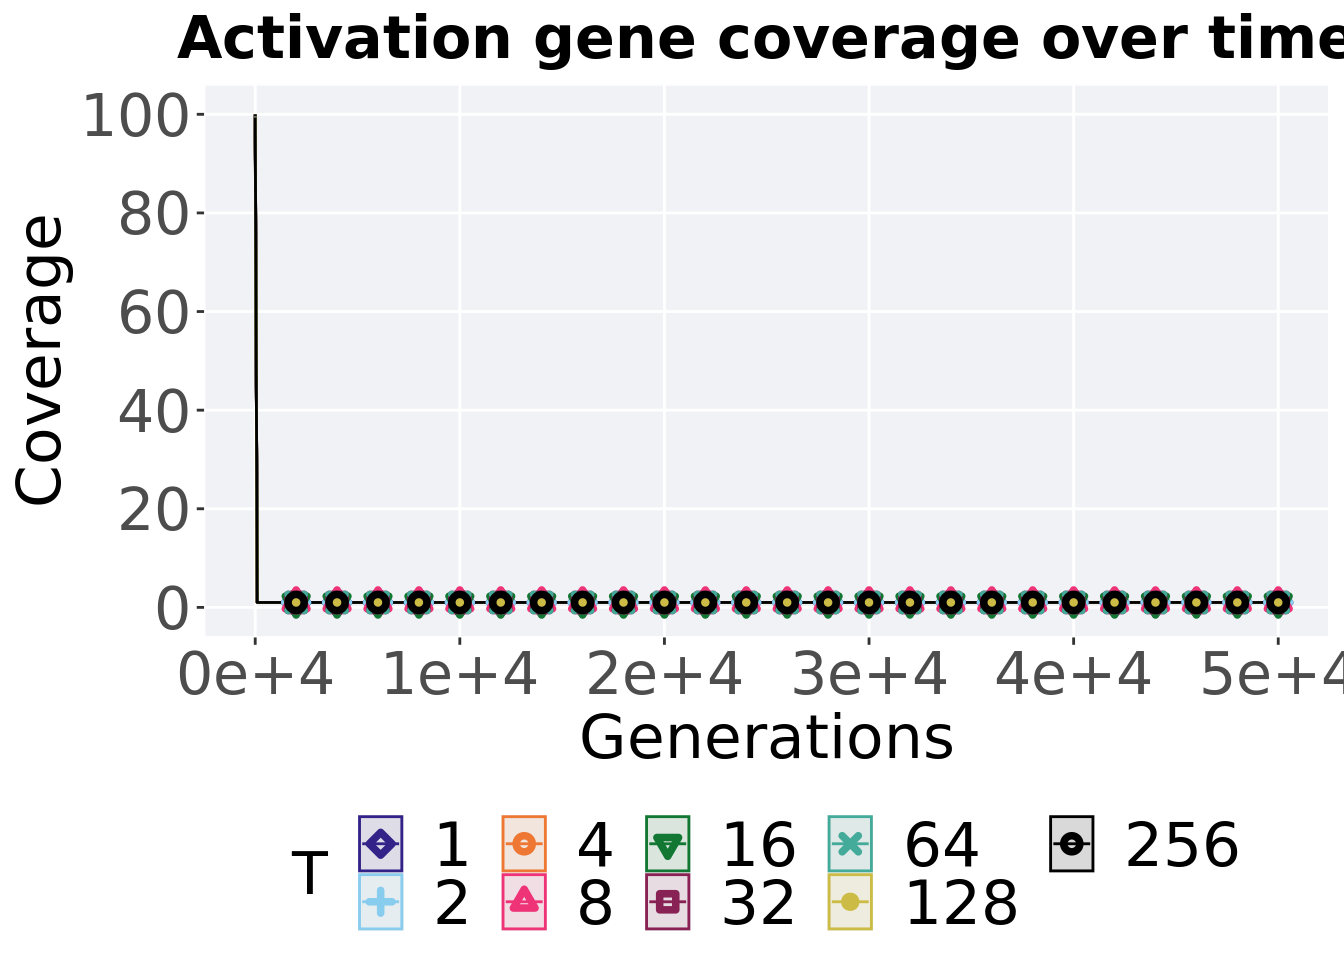
\includegraphics{demo_files/figure-latex/tru-con-act-1.pdf}

\hypertarget{end-of-50000-generations-6}{%
\subsubsection{End of 50,000 generations}\label{end-of-50000-generations-6}}

Activation gene coverage in the population at the end of 50,000 generations.

\begin{Shaded}
\begin{Highlighting}[]
\KeywordTok{filter}\NormalTok{(tru_ot, diagnostic }\OperatorTok{==}\StringTok{ 'contradictory_objectives'} \OperatorTok{&}\StringTok{ }\NormalTok{gen }\OperatorTok{==}\StringTok{ }\DecValTok{50000}\NormalTok{) }\OperatorTok
\KeywordTok{ggplot}\NormalTok{(., }\KeywordTok{aes}\NormalTok{(}\DataTypeTok{x =}\NormalTok{ T, }\DataTypeTok{y =}\NormalTok{ uni_str_pos, }\DataTypeTok{color =}\NormalTok{ T, }\DataTypeTok{fill =}\NormalTok{ T, }\DataTypeTok{shape =}\NormalTok{ T)) }\OperatorTok{+}
\StringTok{  }\KeywordTok{geom_flat_violin}\NormalTok{(}\DataTypeTok{position =} \KeywordTok{position_nudge}\NormalTok{(}\DataTypeTok{x =} \FloatTok{.2}\NormalTok{, }\DataTypeTok{y =} \DecValTok{0}\NormalTok{), }\DataTypeTok{scale =} \StringTok{'width'}\NormalTok{, }\DataTypeTok{alpha =} \FloatTok{0.2}\NormalTok{) }\OperatorTok{+}
\StringTok{  }\KeywordTok{geom_point}\NormalTok{(}\DataTypeTok{position =} \KeywordTok{position_jitter}\NormalTok{(}\DataTypeTok{width =} \FloatTok{.1}\NormalTok{), }\DataTypeTok{size =} \FloatTok{1.5}\NormalTok{, }\DataTypeTok{alpha =} \FloatTok{1.0}\NormalTok{) }\OperatorTok{+}
\StringTok{  }\KeywordTok{geom_boxplot}\NormalTok{(}\DataTypeTok{color =} \StringTok{'black'}\NormalTok{, }\DataTypeTok{width =} \FloatTok{.2}\NormalTok{, }\DataTypeTok{outlier.shape =} \OtherTok{NA}\NormalTok{, }\DataTypeTok{alpha =} \FloatTok{0.0}\NormalTok{) }\OperatorTok{+}
\StringTok{  }\KeywordTok{scale_y_continuous}\NormalTok{(}
    \DataTypeTok{name=}\StringTok{"Coverage"}
\NormalTok{  ) }\OperatorTok{+}
\StringTok{  }\KeywordTok{scale_x_discrete}\NormalTok{(}
    \DataTypeTok{name=}\StringTok{"T"}
\NormalTok{  )}\OperatorTok{+}
\StringTok{  }\KeywordTok{scale_shape_manual}\NormalTok{(}\DataTypeTok{values=}\NormalTok{SHAPE)}\OperatorTok{+}
\StringTok{  }\KeywordTok{scale_colour_manual}\NormalTok{(}\DataTypeTok{values =}\NormalTok{ cb_palette) }\OperatorTok{+}
\StringTok{  }\KeywordTok{scale_fill_manual}\NormalTok{(}\DataTypeTok{values =}\NormalTok{ cb_palette) }\OperatorTok{+}
\StringTok{  }\KeywordTok{ggtitle}\NormalTok{(}\StringTok{"Final activation gene coverage"}\NormalTok{) }\OperatorTok{+}
\StringTok{  }\NormalTok{p_theme}
\end{Highlighting}
\end{Shaded}

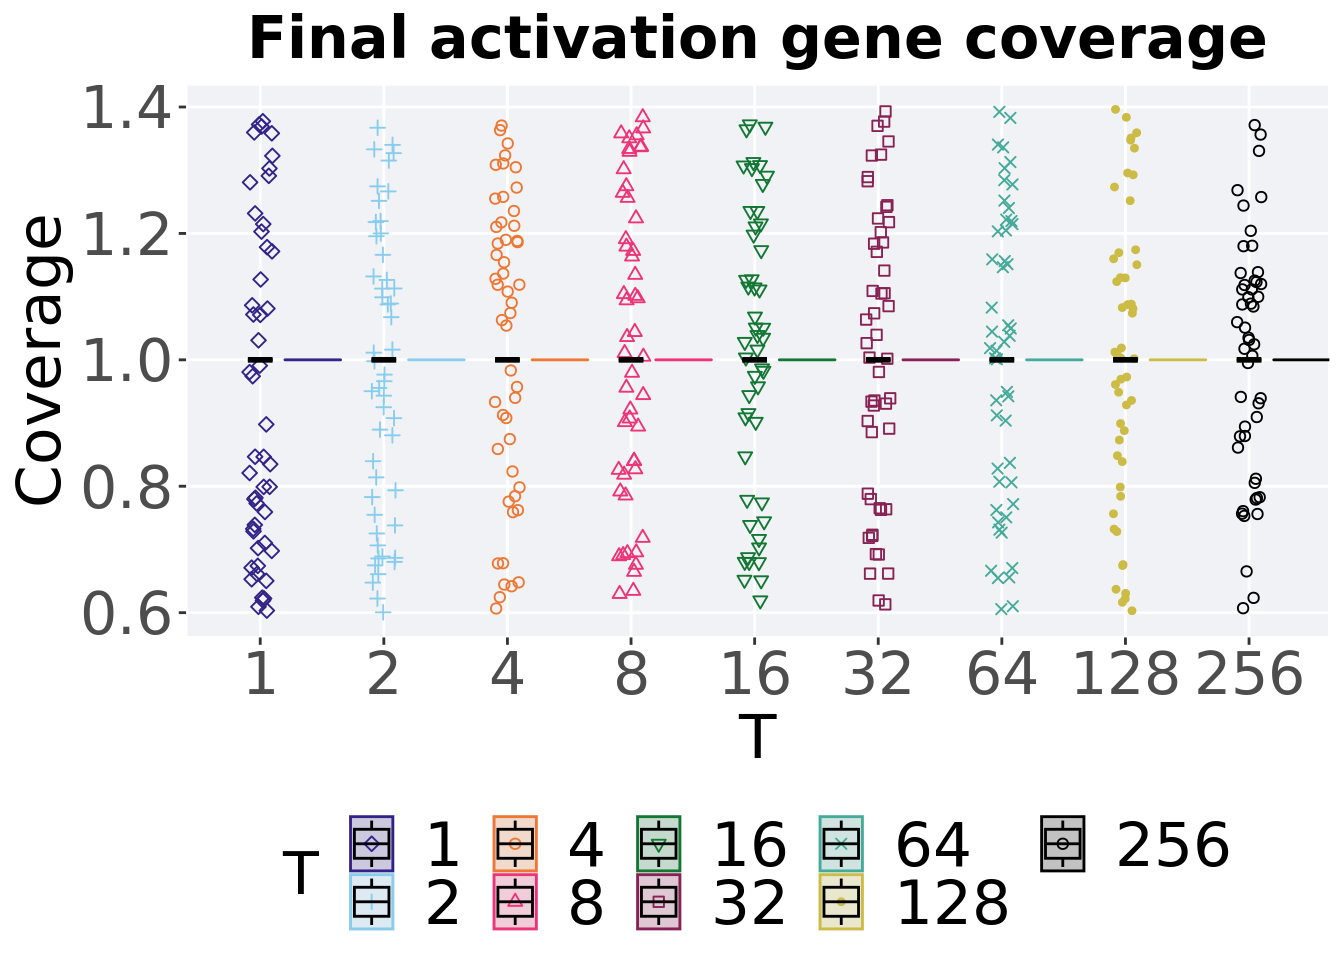
\includegraphics{demo_files/figure-latex/tru-con-act-end-1.pdf}

\hypertarget{stats-28}{%
\paragraph{Stats}\label{stats-28}}

Summary statistics for activation gene coverage in the population at the end of 50,000 generations.

\begin{Shaded}
\begin{Highlighting}[]
\NormalTok{coverage =}\StringTok{ }\KeywordTok{filter}\NormalTok{(tru_ot, diagnostic }\OperatorTok{==}\StringTok{ 'contradictory_objectives'} \OperatorTok{&}\StringTok{ }\NormalTok{gen }\OperatorTok{==}\StringTok{ }\DecValTok{50000}\NormalTok{)}
\KeywordTok{group_by}\NormalTok{(coverage, T) }\OperatorTok
\StringTok{  }\NormalTok{dplyr}\OperatorTok{::}\KeywordTok{summarise}\NormalTok{(}
    \DataTypeTok{count =} \KeywordTok{n}\NormalTok{(),}
    \DataTypeTok{na_cnt =} \KeywordTok{sum}\NormalTok{(}\KeywordTok{is.na}\NormalTok{(uni_str_pos)),}
    \DataTypeTok{min =} \KeywordTok{min}\NormalTok{(uni_str_pos, }\DataTypeTok{na.rm =} \OtherTok{TRUE}\NormalTok{),}
    \DataTypeTok{median =} \KeywordTok{median}\NormalTok{(uni_str_pos, }\DataTypeTok{na.rm =} \OtherTok{TRUE}\NormalTok{),}
    \DataTypeTok{mean =} \KeywordTok{mean}\NormalTok{(uni_str_pos, }\DataTypeTok{na.rm =} \OtherTok{TRUE}\NormalTok{),}
    \DataTypeTok{max =} \KeywordTok{max}\NormalTok{(uni_str_pos, }\DataTypeTok{na.rm =} \OtherTok{TRUE}\NormalTok{),}
    \DataTypeTok{IQR =} \KeywordTok{IQR}\NormalTok{(uni_str_pos, }\DataTypeTok{na.rm =} \OtherTok{TRUE}\NormalTok{)}
\NormalTok{  )}
\end{Highlighting}
\end{Shaded}

\begin{verbatim}
## # A tibble: 9 x 8
##   T     count na_cnt   min median  mean   max   IQR
##   <fct> <int>  <int> <int>  <dbl> <dbl> <int> <dbl>
## 1 1        50      0     1      1     1     1     0
## 2 2        50      0     1      1     1     1     0
## 3 4        50      0     1      1     1     1     0
## 4 8        50      0     1      1     1     1     0
## 5 16       50      0     1      1     1     1     0
## 6 32       50      0     1      1     1     1     0
## 7 64       50      0     1      1     1     1     0
## 8 128      50      0     1      1     1     1     0
## 9 256      50      0     1      1     1     1     0
\end{verbatim}

\hypertarget{multi-valley-crossing-2}{%
\subsection{Multi-valley crossing}\label{multi-valley-crossing-2}}

\hypertarget{satisfactory-trait-coverage-over-time}{%
\subsubsection{Satisfactory trait coverage over time}\label{satisfactory-trait-coverage-over-time}}

\begin{Shaded}
\begin{Highlighting}[]
\NormalTok{lines =}\StringTok{ }\KeywordTok{filter}\NormalTok{(tru_ot_mvc, diagnostic }\OperatorTok{==}\StringTok{ 'contradictory_objectives'}\NormalTok{) }\OperatorTok
\StringTok{  }\KeywordTok{group_by}\NormalTok{(T, gen) }\OperatorTok
\StringTok{  }\NormalTok{dplyr}\OperatorTok{::}\KeywordTok{summarise}\NormalTok{(}
    \DataTypeTok{min =} \KeywordTok{min}\NormalTok{(pop_uni_obj),}
    \DataTypeTok{mean =} \KeywordTok{mean}\NormalTok{(pop_uni_obj),}
    \DataTypeTok{max =} \KeywordTok{max}\NormalTok{(pop_uni_obj)}
\NormalTok{  )}
\end{Highlighting}
\end{Shaded}

\begin{verbatim}
## `summarise()` has grouped output by 'T'. You can override using the `.groups`
## argument.
\end{verbatim}

\begin{Shaded}
\begin{Highlighting}[]
\KeywordTok{ggplot}\NormalTok{(lines, }\KeywordTok{aes}\NormalTok{(}\DataTypeTok{x=}\NormalTok{gen, }\DataTypeTok{y=}\NormalTok{mean, }\DataTypeTok{group =}\NormalTok{ T, }\DataTypeTok{fill =}\NormalTok{T, }\DataTypeTok{color =}\NormalTok{ T, }\DataTypeTok{shape =}\NormalTok{ T)) }\OperatorTok{+}
\StringTok{  }\KeywordTok{geom_ribbon}\NormalTok{(}\KeywordTok{aes}\NormalTok{(}\DataTypeTok{ymin =}\NormalTok{ min, }\DataTypeTok{ymax =}\NormalTok{ max), }\DataTypeTok{alpha =} \FloatTok{0.1}\NormalTok{) }\OperatorTok{+}
\StringTok{  }\KeywordTok{geom_line}\NormalTok{(}\DataTypeTok{size =} \FloatTok{0.5}\NormalTok{) }\OperatorTok{+}
\StringTok{  }\KeywordTok{geom_point}\NormalTok{(}\DataTypeTok{data =} \KeywordTok{filter}\NormalTok{(lines, gen }\OperatorTok\StringTok{ }\DecValTok{2000} \OperatorTok{==}\StringTok{ }\DecValTok{0} \OperatorTok{&}\StringTok{ }\NormalTok{gen }\OperatorTok{!=}\StringTok{ }\DecValTok{0}\NormalTok{), }\DataTypeTok{size =} \FloatTok{1.5}\NormalTok{, }\DataTypeTok{stroke =} \FloatTok{2.0}\NormalTok{, }\DataTypeTok{alpha =} \FloatTok{1.0}\NormalTok{) }\OperatorTok{+}
\StringTok{  }\KeywordTok{scale_y_continuous}\NormalTok{(}
    \DataTypeTok{name=}\StringTok{"Coverage"}
\NormalTok{  ) }\OperatorTok{+}
\StringTok{  }\KeywordTok{scale_x_continuous}\NormalTok{(}
    \DataTypeTok{name=}\StringTok{"Generations"}\NormalTok{,}
    \DataTypeTok{limits=}\KeywordTok{c}\NormalTok{(}\DecValTok{0}\NormalTok{, }\DecValTok{50000}\NormalTok{),}
    \DataTypeTok{breaks=}\KeywordTok{c}\NormalTok{(}\DecValTok{0}\NormalTok{, }\DecValTok{10000}\NormalTok{, }\DecValTok{20000}\NormalTok{, }\DecValTok{30000}\NormalTok{, }\DecValTok{40000}\NormalTok{, }\DecValTok{50000}\NormalTok{),}
    \DataTypeTok{labels=}\KeywordTok{c}\NormalTok{(}\StringTok{"0e+4"}\NormalTok{, }\StringTok{"1e+4"}\NormalTok{, }\StringTok{"2e+4"}\NormalTok{, }\StringTok{"3e+4"}\NormalTok{, }\StringTok{"4e+4"}\NormalTok{, }\StringTok{"5e+4"}\NormalTok{)}

\NormalTok{  ) }\OperatorTok{+}
\StringTok{  }\KeywordTok{scale_shape_manual}\NormalTok{(}\DataTypeTok{values=}\NormalTok{SHAPE)}\OperatorTok{+}
\StringTok{  }\KeywordTok{scale_colour_manual}\NormalTok{(}\DataTypeTok{values =}\NormalTok{ cb_palette) }\OperatorTok{+}
\StringTok{  }\KeywordTok{scale_fill_manual}\NormalTok{(}\DataTypeTok{values =}\NormalTok{ cb_palette) }\OperatorTok{+}
\StringTok{  }\KeywordTok{ggtitle}\NormalTok{(}\StringTok{"Satisfactory trait coverage over time"}\NormalTok{) }\OperatorTok{+}
\StringTok{  }\NormalTok{p_theme}
\end{Highlighting}
\end{Shaded}

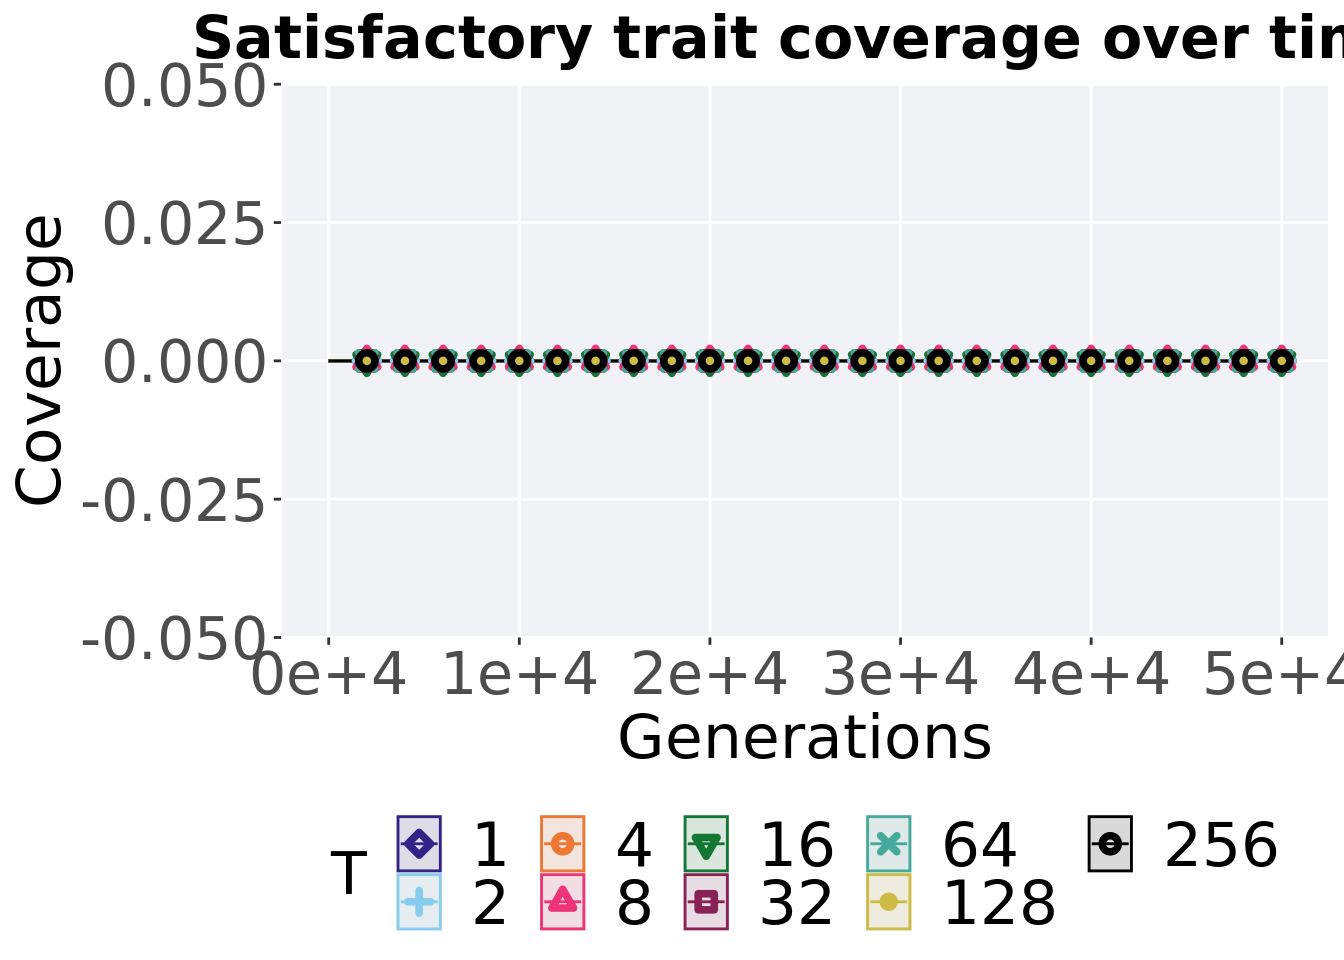
\includegraphics{demo_files/figure-latex/tru-con-mvc-sat-ot-1.pdf}

\hypertarget{satisfactory-trait-coverage-comparison}{%
\subsubsection{Satisfactory trait coverage comparison}\label{satisfactory-trait-coverage-comparison}}

Best performances in the population at 40,000 and 50,000 generations.

\begin{Shaded}
\begin{Highlighting}[]
\CommentTok{# 80% and final generation comparison}
\NormalTok{end =}\StringTok{ }\KeywordTok{filter}\NormalTok{(tru_ot_mvc, diagnostic }\OperatorTok{==}\StringTok{ 'contradictory_objectives'} \OperatorTok{&}\StringTok{ }\NormalTok{gen }\OperatorTok{==}\StringTok{ }\DecValTok{50000}\NormalTok{)}
\NormalTok{end}\OperatorTok{$}\NormalTok{Generation <-}\StringTok{ }\KeywordTok{factor}\NormalTok{(end}\OperatorTok{$}\NormalTok{gen)}

\NormalTok{mid =}\StringTok{ }\KeywordTok{filter}\NormalTok{(tru_ot_mvc, diagnostic }\OperatorTok{==}\StringTok{ 'contradictory_objectives'} \OperatorTok{&}\StringTok{ }\NormalTok{gen }\OperatorTok{==}\StringTok{ }\DecValTok{40000}\NormalTok{)}
\NormalTok{mid}\OperatorTok{$}\NormalTok{Generation <-}\StringTok{ }\KeywordTok{factor}\NormalTok{(mid}\OperatorTok{$}\NormalTok{gen)}

\NormalTok{mvc_p =}\StringTok{ }\KeywordTok{ggplot}\NormalTok{(mid, }\KeywordTok{aes}\NormalTok{(}\DataTypeTok{x =}\NormalTok{ T, }\DataTypeTok{y=}\NormalTok{pop_uni_obj, }\DataTypeTok{group =}\NormalTok{ T, }\DataTypeTok{shape =}\NormalTok{ Generation)) }\OperatorTok{+}
\StringTok{  }\KeywordTok{geom_point}\NormalTok{(}\DataTypeTok{col =}\NormalTok{ mvc_col[}\DecValTok{1}\NormalTok{] , }\DataTypeTok{position =} \KeywordTok{position_jitternudge}\NormalTok{(}\DataTypeTok{jitter.width =} \FloatTok{.03}\NormalTok{, }\DataTypeTok{nudge.x =} \FloatTok{-0.05}\NormalTok{), }\DataTypeTok{size =} \DecValTok{2}\NormalTok{, }\DataTypeTok{alpha =} \FloatTok{1.0}\NormalTok{) }\OperatorTok{+}
\StringTok{  }\KeywordTok{geom_boxplot}\NormalTok{(}\DataTypeTok{position =} \KeywordTok{position_nudge}\NormalTok{(}\DataTypeTok{x =} \FloatTok{-.15}\NormalTok{, }\DataTypeTok{y =} \DecValTok{0}\NormalTok{), }\DataTypeTok{lwd =} \FloatTok{0.7}\NormalTok{, }\DataTypeTok{col =}\NormalTok{ mvc_col[}\DecValTok{1}\NormalTok{], }\DataTypeTok{fill =}\NormalTok{ mvc_col[}\DecValTok{1}\NormalTok{], }\DataTypeTok{width =} \FloatTok{.1}\NormalTok{, }\DataTypeTok{outlier.shape =} \OtherTok{NA}\NormalTok{, }\DataTypeTok{alpha =} \FloatTok{0.0}\NormalTok{) }\OperatorTok{+}

\StringTok{  }\KeywordTok{geom_point}\NormalTok{(}\DataTypeTok{data =}\NormalTok{ end, }\KeywordTok{aes}\NormalTok{(}\DataTypeTok{x =}\NormalTok{ T, }\DataTypeTok{y=}\NormalTok{pop_uni_obj), }\DataTypeTok{col =}\NormalTok{ mvc_col[}\DecValTok{2}\NormalTok{], }\DataTypeTok{position =} \KeywordTok{position_jitternudge}\NormalTok{(}\DataTypeTok{jitter.width =} \FloatTok{.03}\NormalTok{, }\DataTypeTok{nudge.x =} \FloatTok{0.05}\NormalTok{), }\DataTypeTok{size =} \DecValTok{2}\NormalTok{, }\DataTypeTok{alpha =} \FloatTok{1.0}\NormalTok{) }\OperatorTok{+}
\StringTok{  }\KeywordTok{geom_boxplot}\NormalTok{(}\DataTypeTok{data =}\NormalTok{ end, }\KeywordTok{aes}\NormalTok{(}\DataTypeTok{x =}\NormalTok{ T, }\DataTypeTok{y=}\NormalTok{pop_uni_obj), }\DataTypeTok{position =} \KeywordTok{position_nudge}\NormalTok{(}\DataTypeTok{x =} \FloatTok{.15}\NormalTok{, }\DataTypeTok{y =} \DecValTok{0}\NormalTok{), }\DataTypeTok{lwd =} \FloatTok{0.7}\NormalTok{, }\DataTypeTok{col =}\NormalTok{ mvc_col[}\DecValTok{2}\NormalTok{], }\DataTypeTok{fill =}\NormalTok{ mvc_col[}\DecValTok{2}\NormalTok{], }\DataTypeTok{width =} \FloatTok{.1}\NormalTok{, }\DataTypeTok{outlier.shape =} \OtherTok{NA}\NormalTok{, }\DataTypeTok{alpha =} \FloatTok{0.0}\NormalTok{) }\OperatorTok{+}

\StringTok{  }\KeywordTok{scale_y_continuous}\NormalTok{(}
    \DataTypeTok{name=}\StringTok{"Coverage"}\NormalTok{,}
\NormalTok{  ) }\OperatorTok{+}
\StringTok{  }\KeywordTok{scale_x_discrete}\NormalTok{(}
    \DataTypeTok{name=}\StringTok{"T"}
\NormalTok{  )}\OperatorTok{+}
\StringTok{  }\KeywordTok{scale_shape_manual}\NormalTok{(}\DataTypeTok{values=}\KeywordTok{c}\NormalTok{(}\DecValTok{0}\NormalTok{,}\DecValTok{1}\NormalTok{))}\OperatorTok{+}
\StringTok{  }\KeywordTok{scale_colour_manual}\NormalTok{(}\DataTypeTok{values =} \KeywordTok{c}\NormalTok{(mvc_col[}\DecValTok{1}\NormalTok{],mvc_col[}\DecValTok{2}\NormalTok{])) }\OperatorTok{+}
\StringTok{  }\NormalTok{p_theme}

\KeywordTok{plot_grid}\NormalTok{(}
\NormalTok{  mvc_p }\OperatorTok{+}
\StringTok{    }\KeywordTok{ggtitle}\NormalTok{(}\StringTok{"Satisfactory trait coverage"}\NormalTok{) }\OperatorTok{+}
\StringTok{    }\KeywordTok{theme}\NormalTok{(}\DataTypeTok{legend.position=}\StringTok{"none"}\NormalTok{),}
\NormalTok{  legend,}
  \DataTypeTok{nrow=}\DecValTok{2}\NormalTok{,}
  \DataTypeTok{rel_heights =} \KeywordTok{c}\NormalTok{(}\DecValTok{1}\NormalTok{,.}\DecValTok{05}\NormalTok{),}
  \DataTypeTok{label_size =}\NormalTok{ TSIZE}
\NormalTok{)}
\end{Highlighting}
\end{Shaded}

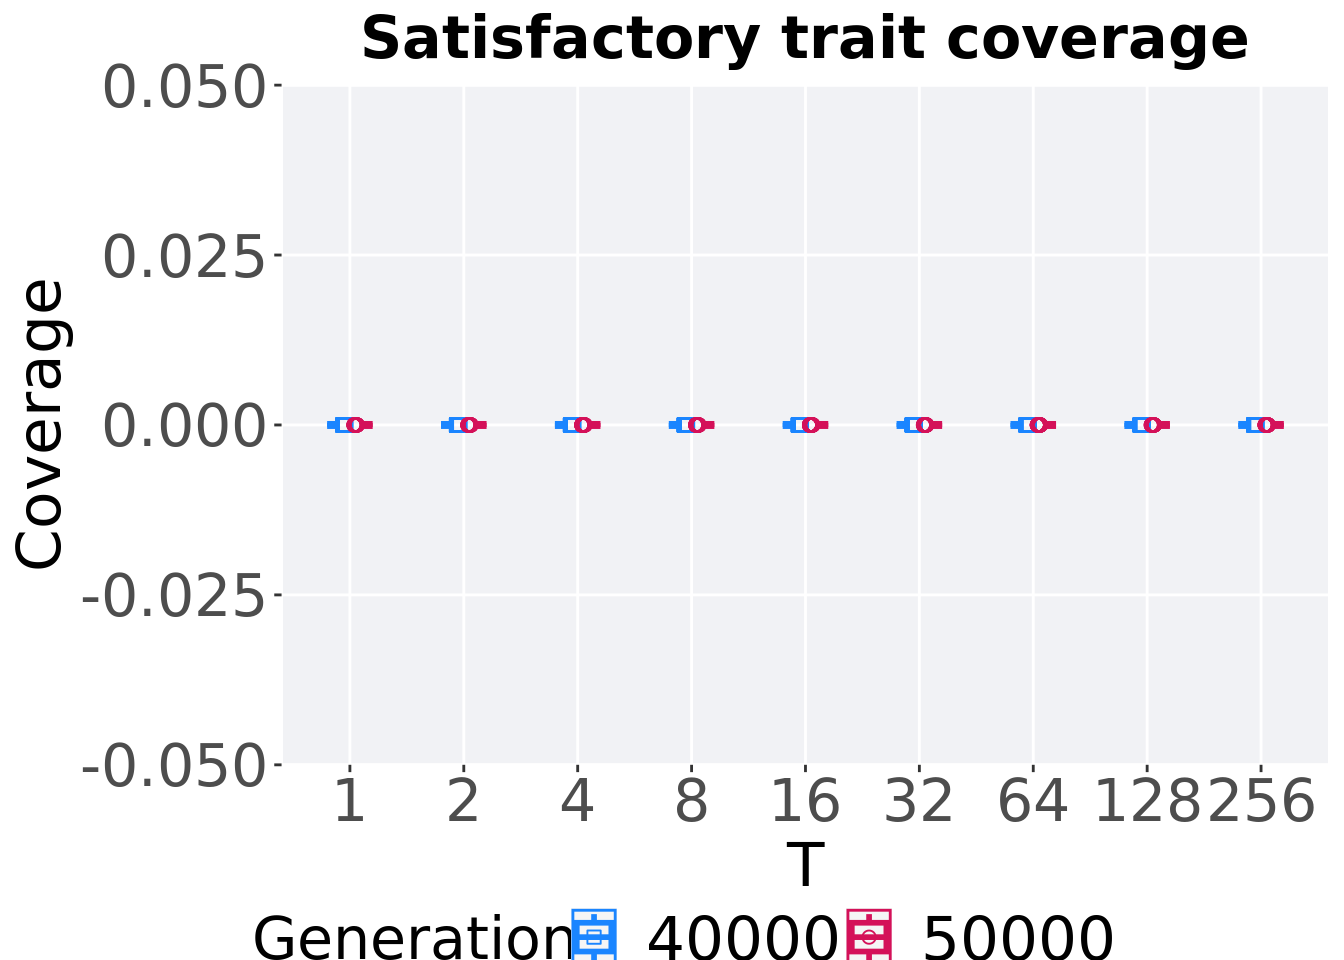
\includegraphics{demo_files/figure-latex/tru-con-mvc-sat-sli-1.pdf}

\hypertarget{stats-29}{%
\paragraph{Stats}\label{stats-29}}

Summary statistics for the performance of the best performance at 40,000 and 50,000 generations.

\begin{Shaded}
\begin{Highlighting}[]
\NormalTok{slices =}\StringTok{ }\KeywordTok{filter}\NormalTok{(tru_ot_mvc, diagnostic }\OperatorTok{==}\StringTok{ 'contradictory_objectives'} \OperatorTok{&}\StringTok{ }\NormalTok{(gen }\OperatorTok{==}\StringTok{ }\DecValTok{50000} \OperatorTok{|}\StringTok{ }\NormalTok{gen }\OperatorTok{==}\StringTok{ }\DecValTok{40000}\NormalTok{))}
\NormalTok{slices}\OperatorTok{$}\NormalTok{Generation <-}\StringTok{ }\KeywordTok{factor}\NormalTok{(slices}\OperatorTok{$}\NormalTok{gen, }\DataTypeTok{levels =} \KeywordTok{c}\NormalTok{(}\DecValTok{50000}\NormalTok{,}\DecValTok{40000}\NormalTok{))}
\NormalTok{slices }\OperatorTok
\StringTok{  }\KeywordTok{group_by}\NormalTok{(T, Generation) }\OperatorTok
\StringTok{  }\NormalTok{dplyr}\OperatorTok{::}\KeywordTok{summarise}\NormalTok{(}
    \DataTypeTok{count =} \KeywordTok{n}\NormalTok{(),}
    \DataTypeTok{na_cnt =} \KeywordTok{sum}\NormalTok{(}\KeywordTok{is.na}\NormalTok{(pop_uni_obj)),}
    \DataTypeTok{min =} \KeywordTok{min}\NormalTok{(pop_uni_obj, }\DataTypeTok{na.rm =} \OtherTok{TRUE}\NormalTok{),}
    \DataTypeTok{median =} \KeywordTok{median}\NormalTok{(pop_uni_obj, }\DataTypeTok{na.rm =} \OtherTok{TRUE}\NormalTok{),}
    \DataTypeTok{mean =} \KeywordTok{mean}\NormalTok{(pop_uni_obj, }\DataTypeTok{na.rm =} \OtherTok{TRUE}\NormalTok{),}
    \DataTypeTok{max =} \KeywordTok{max}\NormalTok{(pop_uni_obj, }\DataTypeTok{na.rm =} \OtherTok{TRUE}\NormalTok{),}
    \DataTypeTok{IQR =} \KeywordTok{IQR}\NormalTok{(pop_uni_obj, }\DataTypeTok{na.rm =} \OtherTok{TRUE}\NormalTok{)}
\NormalTok{  )}
\end{Highlighting}
\end{Shaded}

\begin{verbatim}
## `summarise()` has grouped output by 'T'. You can override using the `.groups`
## argument.
\end{verbatim}

\begin{verbatim}
## # A tibble: 18 x 9
## # Groups:   T [9]
##    T     Generation count na_cnt   min median  mean   max   IQR
##    <fct> <fct>      <int>  <int> <int>  <dbl> <dbl> <int> <dbl>
##  1 1     50000         50      0     0      0     0     0     0
##  2 1     40000         50      0     0      0     0     0     0
##  3 2     50000         50      0     0      0     0     0     0
##  4 2     40000         50      0     0      0     0     0     0
##  5 4     50000         50      0     0      0     0     0     0
##  6 4     40000         50      0     0      0     0     0     0
##  7 8     50000         50      0     0      0     0     0     0
##  8 8     40000         50      0     0      0     0     0     0
##  9 16    50000         50      0     0      0     0     0     0
## 10 16    40000         50      0     0      0     0     0     0
## 11 32    50000         50      0     0      0     0     0     0
## 12 32    40000         50      0     0      0     0     0     0
## 13 64    50000         50      0     0      0     0     0     0
## 14 64    40000         50      0     0      0     0     0     0
## 15 128   50000         50      0     0      0     0     0     0
## 16 128   40000         50      0     0      0     0     0     0
## 17 256   50000         50      0     0      0     0     0     0
## 18 256   40000         50      0     0      0     0     0     0
\end{verbatim}

T 2

\begin{Shaded}
\begin{Highlighting}[]
\KeywordTok{wilcox.test}\NormalTok{(}\DataTypeTok{x =} \KeywordTok{filter}\NormalTok{(slices, T }\OperatorTok{==}\StringTok{ }\DecValTok{2} \OperatorTok{&}\StringTok{ }\NormalTok{Generation }\OperatorTok{==}\StringTok{ }\DecValTok{50000}\NormalTok{)}\OperatorTok{$}\NormalTok{pop_uni_obj,}
            \DataTypeTok{y =} \KeywordTok{filter}\NormalTok{(slices, T }\OperatorTok{==}\StringTok{ }\DecValTok{2} \OperatorTok{&}\StringTok{ }\NormalTok{Generation }\OperatorTok{==}\StringTok{ }\DecValTok{40000}\NormalTok{)}\OperatorTok{$}\NormalTok{pop_uni_obj,}
            \DataTypeTok{alternative =} \StringTok{'t'}\NormalTok{)}
\end{Highlighting}
\end{Shaded}

\begin{verbatim}
## 
##  Wilcoxon rank sum test with continuity correction
## 
## data:  filter(slices, T == 2 & Generation == 50000)$pop_uni_obj and filter(slices, T == 2 & Generation == 40000)$pop_uni_obj
## W = 1250, p-value = NA
## alternative hypothesis: true location shift is not equal to 0
\end{verbatim}

T 4

\begin{Shaded}
\begin{Highlighting}[]
\KeywordTok{wilcox.test}\NormalTok{(}\DataTypeTok{x =} \KeywordTok{filter}\NormalTok{(slices, T }\OperatorTok{==}\StringTok{ }\DecValTok{4} \OperatorTok{&}\StringTok{ }\NormalTok{Generation }\OperatorTok{==}\StringTok{ }\DecValTok{50000}\NormalTok{)}\OperatorTok{$}\NormalTok{pop_uni_obj,}
            \DataTypeTok{y =} \KeywordTok{filter}\NormalTok{(slices, T }\OperatorTok{==}\StringTok{ }\DecValTok{4} \OperatorTok{&}\StringTok{ }\NormalTok{Generation }\OperatorTok{==}\StringTok{ }\DecValTok{40000}\NormalTok{)}\OperatorTok{$}\NormalTok{pop_uni_obj,}
            \DataTypeTok{alternative =} \StringTok{'t'}\NormalTok{)}
\end{Highlighting}
\end{Shaded}

\begin{verbatim}
## 
##  Wilcoxon rank sum test with continuity correction
## 
## data:  filter(slices, T == 4 & Generation == 50000)$pop_uni_obj and filter(slices, T == 4 & Generation == 40000)$pop_uni_obj
## W = 1250, p-value = NA
## alternative hypothesis: true location shift is not equal to 0
\end{verbatim}

T 8

\begin{Shaded}
\begin{Highlighting}[]
\KeywordTok{wilcox.test}\NormalTok{(}\DataTypeTok{x =} \KeywordTok{filter}\NormalTok{(slices, T }\OperatorTok{==}\StringTok{ }\DecValTok{8} \OperatorTok{&}\StringTok{ }\NormalTok{Generation }\OperatorTok{==}\StringTok{ }\DecValTok{50000}\NormalTok{)}\OperatorTok{$}\NormalTok{pop_uni_obj,}
            \DataTypeTok{y =} \KeywordTok{filter}\NormalTok{(slices, T }\OperatorTok{==}\StringTok{ }\DecValTok{8} \OperatorTok{&}\StringTok{ }\NormalTok{Generation }\OperatorTok{==}\StringTok{ }\DecValTok{40000}\NormalTok{)}\OperatorTok{$}\NormalTok{pop_uni_obj,}
            \DataTypeTok{alternative =} \StringTok{'t'}\NormalTok{)}
\end{Highlighting}
\end{Shaded}

\begin{verbatim}
## 
##  Wilcoxon rank sum test with continuity correction
## 
## data:  filter(slices, T == 8 & Generation == 50000)$pop_uni_obj and filter(slices, T == 8 & Generation == 40000)$pop_uni_obj
## W = 1250, p-value = NA
## alternative hypothesis: true location shift is not equal to 0
\end{verbatim}

T 16

\begin{Shaded}
\begin{Highlighting}[]
\KeywordTok{wilcox.test}\NormalTok{(}\DataTypeTok{x =} \KeywordTok{filter}\NormalTok{(slices, T }\OperatorTok{==}\StringTok{ }\DecValTok{16} \OperatorTok{&}\StringTok{ }\NormalTok{Generation }\OperatorTok{==}\StringTok{ }\DecValTok{50000}\NormalTok{)}\OperatorTok{$}\NormalTok{pop_uni_obj,}
            \DataTypeTok{y =} \KeywordTok{filter}\NormalTok{(slices, T }\OperatorTok{==}\StringTok{ }\DecValTok{16} \OperatorTok{&}\StringTok{ }\NormalTok{Generation }\OperatorTok{==}\StringTok{ }\DecValTok{40000}\NormalTok{)}\OperatorTok{$}\NormalTok{pop_uni_obj,}
            \DataTypeTok{alternative =} \StringTok{'t'}\NormalTok{)}
\end{Highlighting}
\end{Shaded}

\begin{verbatim}
## 
##  Wilcoxon rank sum test with continuity correction
## 
## data:  filter(slices, T == 16 & Generation == 50000)$pop_uni_obj and filter(slices, T == 16 & Generation == 40000)$pop_uni_obj
## W = 1250, p-value = NA
## alternative hypothesis: true location shift is not equal to 0
\end{verbatim}

T 32

\begin{Shaded}
\begin{Highlighting}[]
\KeywordTok{wilcox.test}\NormalTok{(}\DataTypeTok{x =} \KeywordTok{filter}\NormalTok{(slices, T }\OperatorTok{==}\StringTok{ }\DecValTok{32} \OperatorTok{&}\StringTok{ }\NormalTok{Generation }\OperatorTok{==}\StringTok{ }\DecValTok{50000}\NormalTok{)}\OperatorTok{$}\NormalTok{pop_uni_obj,}
            \DataTypeTok{y =} \KeywordTok{filter}\NormalTok{(slices, T }\OperatorTok{==}\StringTok{ }\DecValTok{32} \OperatorTok{&}\StringTok{ }\NormalTok{Generation }\OperatorTok{==}\StringTok{ }\DecValTok{40000}\NormalTok{)}\OperatorTok{$}\NormalTok{pop_uni_obj,}
            \DataTypeTok{alternative =} \StringTok{'t'}\NormalTok{)}
\end{Highlighting}
\end{Shaded}

\begin{verbatim}
## 
##  Wilcoxon rank sum test with continuity correction
## 
## data:  filter(slices, T == 32 & Generation == 50000)$pop_uni_obj and filter(slices, T == 32 & Generation == 40000)$pop_uni_obj
## W = 1250, p-value = NA
## alternative hypothesis: true location shift is not equal to 0
\end{verbatim}

T 64

\begin{Shaded}
\begin{Highlighting}[]
\KeywordTok{wilcox.test}\NormalTok{(}\DataTypeTok{x =} \KeywordTok{filter}\NormalTok{(slices, T }\OperatorTok{==}\StringTok{ }\DecValTok{64} \OperatorTok{&}\StringTok{ }\NormalTok{Generation }\OperatorTok{==}\StringTok{ }\DecValTok{50000}\NormalTok{)}\OperatorTok{$}\NormalTok{pop_uni_obj,}
            \DataTypeTok{y =} \KeywordTok{filter}\NormalTok{(slices, T }\OperatorTok{==}\StringTok{ }\DecValTok{64} \OperatorTok{&}\StringTok{ }\NormalTok{Generation }\OperatorTok{==}\StringTok{ }\DecValTok{40000}\NormalTok{)}\OperatorTok{$}\NormalTok{pop_uni_obj,}
            \DataTypeTok{alternative =} \StringTok{'t'}\NormalTok{)}
\end{Highlighting}
\end{Shaded}

\begin{verbatim}
## 
##  Wilcoxon rank sum test with continuity correction
## 
## data:  filter(slices, T == 64 & Generation == 50000)$pop_uni_obj and filter(slices, T == 64 & Generation == 40000)$pop_uni_obj
## W = 1250, p-value = NA
## alternative hypothesis: true location shift is not equal to 0
\end{verbatim}

T 128

\begin{Shaded}
\begin{Highlighting}[]
\KeywordTok{wilcox.test}\NormalTok{(}\DataTypeTok{x =} \KeywordTok{filter}\NormalTok{(slices, T }\OperatorTok{==}\StringTok{ }\DecValTok{128} \OperatorTok{&}\StringTok{ }\NormalTok{Generation }\OperatorTok{==}\StringTok{ }\DecValTok{50000}\NormalTok{)}\OperatorTok{$}\NormalTok{pop_uni_obj,}
            \DataTypeTok{y =} \KeywordTok{filter}\NormalTok{(slices, T }\OperatorTok{==}\StringTok{ }\DecValTok{128} \OperatorTok{&}\StringTok{ }\NormalTok{Generation }\OperatorTok{==}\StringTok{ }\DecValTok{40000}\NormalTok{)}\OperatorTok{$}\NormalTok{pop_uni_obj,}
            \DataTypeTok{alternative =} \StringTok{'t'}\NormalTok{)}
\end{Highlighting}
\end{Shaded}

\begin{verbatim}
## 
##  Wilcoxon rank sum test with continuity correction
## 
## data:  filter(slices, T == 128 & Generation == 50000)$pop_uni_obj and filter(slices, T == 128 & Generation == 40000)$pop_uni_obj
## W = 1250, p-value = NA
## alternative hypothesis: true location shift is not equal to 0
\end{verbatim}

T 256

\begin{Shaded}
\begin{Highlighting}[]
\KeywordTok{wilcox.test}\NormalTok{(}\DataTypeTok{x =} \KeywordTok{filter}\NormalTok{(slices, T }\OperatorTok{==}\StringTok{ }\DecValTok{256} \OperatorTok{&}\StringTok{ }\NormalTok{Generation }\OperatorTok{==}\StringTok{ }\DecValTok{50000}\NormalTok{)}\OperatorTok{$}\NormalTok{pop_uni_obj,}
            \DataTypeTok{y =} \KeywordTok{filter}\NormalTok{(slices, T }\OperatorTok{==}\StringTok{ }\DecValTok{256} \OperatorTok{&}\StringTok{ }\NormalTok{Generation }\OperatorTok{==}\StringTok{ }\DecValTok{40000}\NormalTok{)}\OperatorTok{$}\NormalTok{pop_uni_obj,}
            \DataTypeTok{alternative =} \StringTok{'t'}\NormalTok{)}
\end{Highlighting}
\end{Shaded}

\begin{verbatim}
## 
##  Wilcoxon rank sum test with continuity correction
## 
## data:  filter(slices, T == 256 & Generation == 50000)$pop_uni_obj and filter(slices, T == 256 & Generation == 40000)$pop_uni_obj
## W = 1250, p-value = NA
## alternative hypothesis: true location shift is not equal to 0
\end{verbatim}

\hypertarget{activation-gene-coverage-over-time}{%
\subsubsection{Activation gene coverage over time}\label{activation-gene-coverage-over-time}}

\begin{Shaded}
\begin{Highlighting}[]
\NormalTok{lines =}\StringTok{ }\KeywordTok{filter}\NormalTok{(tru_ot_mvc, diagnostic }\OperatorTok{==}\StringTok{ 'contradictory_objectives'}\NormalTok{) }\OperatorTok
\StringTok{  }\KeywordTok{group_by}\NormalTok{(T, gen) }\OperatorTok
\StringTok{  }\NormalTok{dplyr}\OperatorTok{::}\KeywordTok{summarise}\NormalTok{(}
    \DataTypeTok{min =} \KeywordTok{min}\NormalTok{(uni_str_pos),}
    \DataTypeTok{mean =} \KeywordTok{mean}\NormalTok{(uni_str_pos),}
    \DataTypeTok{max =} \KeywordTok{max}\NormalTok{(uni_str_pos)}
\NormalTok{  )}
\end{Highlighting}
\end{Shaded}

\begin{verbatim}
## `summarise()` has grouped output by 'T'. You can override using the `.groups`
## argument.
\end{verbatim}

\begin{Shaded}
\begin{Highlighting}[]
\KeywordTok{ggplot}\NormalTok{(lines, }\KeywordTok{aes}\NormalTok{(}\DataTypeTok{x=}\NormalTok{gen, }\DataTypeTok{y=}\NormalTok{mean, }\DataTypeTok{group =}\NormalTok{ T, }\DataTypeTok{fill =}\NormalTok{T, }\DataTypeTok{color =}\NormalTok{ T, }\DataTypeTok{shape =}\NormalTok{ T)) }\OperatorTok{+}
\StringTok{  }\KeywordTok{geom_ribbon}\NormalTok{(}\KeywordTok{aes}\NormalTok{(}\DataTypeTok{ymin =}\NormalTok{ min, }\DataTypeTok{ymax =}\NormalTok{ max), }\DataTypeTok{alpha =} \FloatTok{0.1}\NormalTok{) }\OperatorTok{+}
\StringTok{  }\KeywordTok{geom_line}\NormalTok{(}\DataTypeTok{size =} \FloatTok{0.5}\NormalTok{) }\OperatorTok{+}
\StringTok{  }\KeywordTok{geom_point}\NormalTok{(}\DataTypeTok{data =} \KeywordTok{filter}\NormalTok{(lines, gen }\OperatorTok\StringTok{ }\DecValTok{2000} \OperatorTok{==}\StringTok{ }\DecValTok{0} \OperatorTok{&}\StringTok{ }\NormalTok{gen }\OperatorTok{!=}\StringTok{ }\DecValTok{0}\NormalTok{), }\DataTypeTok{size =} \FloatTok{1.5}\NormalTok{, }\DataTypeTok{stroke =} \FloatTok{2.0}\NormalTok{, }\DataTypeTok{alpha =} \FloatTok{1.0}\NormalTok{) }\OperatorTok{+}
\StringTok{  }\KeywordTok{scale_y_continuous}\NormalTok{(}
    \DataTypeTok{name=}\StringTok{"Coverage"}
\NormalTok{  ) }\OperatorTok{+}
\StringTok{  }\KeywordTok{scale_x_continuous}\NormalTok{(}
    \DataTypeTok{name=}\StringTok{"Generations"}\NormalTok{,}
    \DataTypeTok{limits=}\KeywordTok{c}\NormalTok{(}\DecValTok{0}\NormalTok{, }\DecValTok{50000}\NormalTok{),}
    \DataTypeTok{breaks=}\KeywordTok{c}\NormalTok{(}\DecValTok{0}\NormalTok{, }\DecValTok{10000}\NormalTok{, }\DecValTok{20000}\NormalTok{, }\DecValTok{30000}\NormalTok{, }\DecValTok{40000}\NormalTok{, }\DecValTok{50000}\NormalTok{),}
    \DataTypeTok{labels=}\KeywordTok{c}\NormalTok{(}\StringTok{"0e+4"}\NormalTok{, }\StringTok{"1e+4"}\NormalTok{, }\StringTok{"2e+4"}\NormalTok{, }\StringTok{"3e+4"}\NormalTok{, }\StringTok{"4e+4"}\NormalTok{, }\StringTok{"5e+4"}\NormalTok{)}

\NormalTok{  ) }\OperatorTok{+}
\StringTok{  }\KeywordTok{scale_shape_manual}\NormalTok{(}\DataTypeTok{values=}\NormalTok{SHAPE)}\OperatorTok{+}
\StringTok{  }\KeywordTok{scale_colour_manual}\NormalTok{(}\DataTypeTok{values =}\NormalTok{ cb_palette) }\OperatorTok{+}
\StringTok{  }\KeywordTok{scale_fill_manual}\NormalTok{(}\DataTypeTok{values =}\NormalTok{ cb_palette) }\OperatorTok{+}
\StringTok{  }\KeywordTok{ggtitle}\NormalTok{(}\StringTok{"Activation gene coverage over time"}\NormalTok{) }\OperatorTok{+}
\StringTok{  }\NormalTok{p_theme}
\end{Highlighting}
\end{Shaded}

\includegraphics{demo_files/figure-latex/tru-con-mvc-act-ot-1.pdf}

\hypertarget{activation-gene-coverage-comparison}{%
\subsubsection{Activation gene coverage comparison}\label{activation-gene-coverage-comparison}}

Activation gene coverage in the population at 40,000 and 50,000 generations.

\begin{Shaded}
\begin{Highlighting}[]
\CommentTok{# 80% and final generation comparison}
\NormalTok{end =}\StringTok{ }\KeywordTok{filter}\NormalTok{(tru_ot_mvc, diagnostic }\OperatorTok{==}\StringTok{ 'contradictory_objectives'} \OperatorTok{&}\StringTok{ }\NormalTok{gen }\OperatorTok{==}\StringTok{ }\DecValTok{50000}\NormalTok{)}
\NormalTok{end}\OperatorTok{$}\NormalTok{Generation <-}\StringTok{ }\KeywordTok{factor}\NormalTok{(end}\OperatorTok{$}\NormalTok{gen)}

\NormalTok{mid =}\StringTok{ }\KeywordTok{filter}\NormalTok{(tru_ot_mvc, diagnostic }\OperatorTok{==}\StringTok{ 'contradictory_objectives'} \OperatorTok{&}\StringTok{ }\NormalTok{gen }\OperatorTok{==}\StringTok{ }\DecValTok{40000}\NormalTok{)}
\NormalTok{mid}\OperatorTok{$}\NormalTok{Generation <-}\StringTok{ }\KeywordTok{factor}\NormalTok{(mid}\OperatorTok{$}\NormalTok{gen)}

\NormalTok{mvc_p =}\StringTok{ }\KeywordTok{ggplot}\NormalTok{(mid, }\KeywordTok{aes}\NormalTok{(}\DataTypeTok{x =}\NormalTok{ T, }\DataTypeTok{y=}\NormalTok{uni_str_pos, }\DataTypeTok{group =}\NormalTok{ T, }\DataTypeTok{shape =}\NormalTok{ Generation)) }\OperatorTok{+}
\StringTok{  }\KeywordTok{geom_point}\NormalTok{(}\DataTypeTok{col =}\NormalTok{ mvc_col[}\DecValTok{1}\NormalTok{] , }\DataTypeTok{position =} \KeywordTok{position_jitternudge}\NormalTok{(}\DataTypeTok{jitter.width =} \FloatTok{.03}\NormalTok{, }\DataTypeTok{nudge.x =} \FloatTok{-0.05}\NormalTok{), }\DataTypeTok{size =} \DecValTok{2}\NormalTok{, }\DataTypeTok{alpha =} \FloatTok{1.0}\NormalTok{) }\OperatorTok{+}
\StringTok{  }\KeywordTok{geom_boxplot}\NormalTok{(}\DataTypeTok{position =} \KeywordTok{position_nudge}\NormalTok{(}\DataTypeTok{x =} \FloatTok{-.15}\NormalTok{, }\DataTypeTok{y =} \DecValTok{0}\NormalTok{), }\DataTypeTok{lwd =} \FloatTok{0.7}\NormalTok{, }\DataTypeTok{col =}\NormalTok{ mvc_col[}\DecValTok{1}\NormalTok{], }\DataTypeTok{fill =}\NormalTok{ mvc_col[}\DecValTok{1}\NormalTok{], }\DataTypeTok{width =} \FloatTok{.1}\NormalTok{, }\DataTypeTok{outlier.shape =} \OtherTok{NA}\NormalTok{, }\DataTypeTok{alpha =} \FloatTok{0.0}\NormalTok{) }\OperatorTok{+}

\StringTok{  }\KeywordTok{geom_point}\NormalTok{(}\DataTypeTok{data =}\NormalTok{ end, }\KeywordTok{aes}\NormalTok{(}\DataTypeTok{x =}\NormalTok{ T, }\DataTypeTok{y=}\NormalTok{uni_str_pos), }\DataTypeTok{col =}\NormalTok{ mvc_col[}\DecValTok{2}\NormalTok{], }\DataTypeTok{position =} \KeywordTok{position_jitternudge}\NormalTok{(}\DataTypeTok{jitter.width =} \FloatTok{.03}\NormalTok{, }\DataTypeTok{nudge.x =} \FloatTok{0.05}\NormalTok{), }\DataTypeTok{size =} \DecValTok{2}\NormalTok{, }\DataTypeTok{alpha =} \FloatTok{1.0}\NormalTok{) }\OperatorTok{+}
\StringTok{  }\KeywordTok{geom_boxplot}\NormalTok{(}\DataTypeTok{data =}\NormalTok{ end, }\KeywordTok{aes}\NormalTok{(}\DataTypeTok{x =}\NormalTok{ T, }\DataTypeTok{y=}\NormalTok{uni_str_pos), }\DataTypeTok{position =} \KeywordTok{position_nudge}\NormalTok{(}\DataTypeTok{x =} \FloatTok{.15}\NormalTok{, }\DataTypeTok{y =} \DecValTok{0}\NormalTok{), }\DataTypeTok{lwd =} \FloatTok{0.7}\NormalTok{, }\DataTypeTok{col =}\NormalTok{ mvc_col[}\DecValTok{2}\NormalTok{], }\DataTypeTok{fill =}\NormalTok{ mvc_col[}\DecValTok{2}\NormalTok{], }\DataTypeTok{width =} \FloatTok{.1}\NormalTok{, }\DataTypeTok{outlier.shape =} \OtherTok{NA}\NormalTok{, }\DataTypeTok{alpha =} \FloatTok{0.0}\NormalTok{) }\OperatorTok{+}

\StringTok{  }\KeywordTok{scale_y_continuous}\NormalTok{(}
    \DataTypeTok{name=}\StringTok{"Coverage"}\NormalTok{,}
\NormalTok{  ) }\OperatorTok{+}
\StringTok{  }\KeywordTok{scale_x_discrete}\NormalTok{(}
    \DataTypeTok{name=}\StringTok{"T"}
\NormalTok{  )}\OperatorTok{+}
\StringTok{  }\KeywordTok{scale_shape_manual}\NormalTok{(}\DataTypeTok{values=}\KeywordTok{c}\NormalTok{(}\DecValTok{0}\NormalTok{,}\DecValTok{1}\NormalTok{))}\OperatorTok{+}
\StringTok{  }\KeywordTok{scale_colour_manual}\NormalTok{(}\DataTypeTok{values =} \KeywordTok{c}\NormalTok{(mvc_col[}\DecValTok{1}\NormalTok{],mvc_col[}\DecValTok{2}\NormalTok{])) }\OperatorTok{+}
\StringTok{  }\NormalTok{p_theme}

\KeywordTok{plot_grid}\NormalTok{(}
\NormalTok{  mvc_p }\OperatorTok{+}
\StringTok{    }\KeywordTok{ggtitle}\NormalTok{(}\StringTok{"Activation gene coverage"}\NormalTok{) }\OperatorTok{+}
\StringTok{    }\KeywordTok{theme}\NormalTok{(}\DataTypeTok{legend.position=}\StringTok{"none"}\NormalTok{),}
\NormalTok{  legend,}
  \DataTypeTok{nrow=}\DecValTok{2}\NormalTok{,}
  \DataTypeTok{rel_heights =} \KeywordTok{c}\NormalTok{(}\DecValTok{1}\NormalTok{,.}\DecValTok{05}\NormalTok{),}
  \DataTypeTok{label_size =}\NormalTok{ TSIZE}
\NormalTok{)}
\end{Highlighting}
\end{Shaded}

\includegraphics{demo_files/figure-latex/tru-con-mvc-act-sli-1.pdf}

\hypertarget{stats-30}{%
\paragraph{Stats}\label{stats-30}}

Summary statistics for the activation gene coverage at 40,000 and 50,000 generations.

\begin{Shaded}
\begin{Highlighting}[]
\NormalTok{slices =}\StringTok{ }\KeywordTok{filter}\NormalTok{(tru_ot_mvc, diagnostic }\OperatorTok{==}\StringTok{ 'contradictory_objectives'} \OperatorTok{&}\StringTok{ }\NormalTok{(gen }\OperatorTok{==}\StringTok{ }\DecValTok{50000} \OperatorTok{|}\StringTok{ }\NormalTok{gen }\OperatorTok{==}\StringTok{ }\DecValTok{40000}\NormalTok{))}
\NormalTok{slices}\OperatorTok{$}\NormalTok{Generation <-}\StringTok{ }\KeywordTok{factor}\NormalTok{(slices}\OperatorTok{$}\NormalTok{gen, }\DataTypeTok{levels =} \KeywordTok{c}\NormalTok{(}\DecValTok{50000}\NormalTok{,}\DecValTok{40000}\NormalTok{))}
\NormalTok{slices }\OperatorTok
\StringTok{  }\KeywordTok{group_by}\NormalTok{(T, Generation) }\OperatorTok
\StringTok{  }\NormalTok{dplyr}\OperatorTok{::}\KeywordTok{summarise}\NormalTok{(}
    \DataTypeTok{count =} \KeywordTok{n}\NormalTok{(),}
    \DataTypeTok{na_cnt =} \KeywordTok{sum}\NormalTok{(}\KeywordTok{is.na}\NormalTok{(uni_str_pos)),}
    \DataTypeTok{min =} \KeywordTok{min}\NormalTok{(uni_str_pos, }\DataTypeTok{na.rm =} \OtherTok{TRUE}\NormalTok{),}
    \DataTypeTok{median =} \KeywordTok{median}\NormalTok{(uni_str_pos, }\DataTypeTok{na.rm =} \OtherTok{TRUE}\NormalTok{),}
    \DataTypeTok{mean =} \KeywordTok{mean}\NormalTok{(uni_str_pos, }\DataTypeTok{na.rm =} \OtherTok{TRUE}\NormalTok{),}
    \DataTypeTok{max =} \KeywordTok{max}\NormalTok{(uni_str_pos, }\DataTypeTok{na.rm =} \OtherTok{TRUE}\NormalTok{),}
    \DataTypeTok{IQR =} \KeywordTok{IQR}\NormalTok{(uni_str_pos, }\DataTypeTok{na.rm =} \OtherTok{TRUE}\NormalTok{)}
\NormalTok{  )}
\end{Highlighting}
\end{Shaded}

\begin{verbatim}
## `summarise()` has grouped output by 'T'. You can override using the `.groups`
## argument.
\end{verbatim}

\begin{verbatim}
## # A tibble: 18 x 9
## # Groups:   T [9]
##    T     Generation count na_cnt   min median  mean   max   IQR
##    <fct> <fct>      <int>  <int> <int>  <dbl> <dbl> <int> <dbl>
##  1 1     50000         50      0     1      5  5.68    11  2.75
##  2 1     40000         50      0     2      5  5.54    10  3   
##  3 2     50000         50      0     2      6  5.78    10  3.5 
##  4 2     40000         50      0     1      6  5.64    10  3   
##  5 4     50000         50      0     2      6  6.08    13  3   
##  6 4     40000         50      0     2      6  6.12    14  2.75
##  7 8     50000         50      0     2      5  5.6     11  3   
##  8 8     40000         50      0     2      6  5.8     11  3   
##  9 16    50000         50      0     1      6  6.04    11  2   
## 10 16    40000         50      0     1      5  5.42    11  3   
## 11 32    50000         50      0     1      6  5.94    11  3   
## 12 32    40000         50      0     2      5  5.58    10  3   
## 13 64    50000         50      0     1      5  5.14    11  3.75
## 14 64    40000         50      0     2      5  5.66    11  3   
## 15 128   50000         50      0     1      5  5.1     10  2.75
## 16 128   40000         50      0     1      5  4.78    10  2.75
## 17 256   50000         50      0     2      5  5.12    11  2   
## 18 256   40000         50      0     2      4  4.58     9  1.75
\end{verbatim}

T 2

\begin{Shaded}
\begin{Highlighting}[]
\KeywordTok{wilcox.test}\NormalTok{(}\DataTypeTok{x =} \KeywordTok{filter}\NormalTok{(slices, T }\OperatorTok{==}\StringTok{ }\DecValTok{2} \OperatorTok{&}\StringTok{ }\NormalTok{Generation }\OperatorTok{==}\StringTok{ }\DecValTok{50000}\NormalTok{)}\OperatorTok{$}\NormalTok{uni_str_pos,}
            \DataTypeTok{y =} \KeywordTok{filter}\NormalTok{(slices, T }\OperatorTok{==}\StringTok{ }\DecValTok{2} \OperatorTok{&}\StringTok{ }\NormalTok{Generation }\OperatorTok{==}\StringTok{ }\DecValTok{40000}\NormalTok{)}\OperatorTok{$}\NormalTok{uni_str_pos,}
            \DataTypeTok{alternative =} \StringTok{'t'}\NormalTok{)}
\end{Highlighting}
\end{Shaded}

\begin{verbatim}
## 
##  Wilcoxon rank sum test with continuity correction
## 
## data:  filter(slices, T == 2 & Generation == 50000)$uni_str_pos and filter(slices, T == 2 & Generation == 40000)$uni_str_pos
## W = 1280.5, p-value = 0.8346
## alternative hypothesis: true location shift is not equal to 0
\end{verbatim}

T 4

\begin{Shaded}
\begin{Highlighting}[]
\KeywordTok{wilcox.test}\NormalTok{(}\DataTypeTok{x =} \KeywordTok{filter}\NormalTok{(slices, T }\OperatorTok{==}\StringTok{ }\DecValTok{4} \OperatorTok{&}\StringTok{ }\NormalTok{Generation }\OperatorTok{==}\StringTok{ }\DecValTok{50000}\NormalTok{)}\OperatorTok{$}\NormalTok{uni_str_pos,}
            \DataTypeTok{y =} \KeywordTok{filter}\NormalTok{(slices, T }\OperatorTok{==}\StringTok{ }\DecValTok{4} \OperatorTok{&}\StringTok{ }\NormalTok{Generation }\OperatorTok{==}\StringTok{ }\DecValTok{40000}\NormalTok{)}\OperatorTok{$}\NormalTok{uni_str_pos,}
            \DataTypeTok{alternative =} \StringTok{'t'}\NormalTok{)}
\end{Highlighting}
\end{Shaded}

\begin{verbatim}
## 
##  Wilcoxon rank sum test with continuity correction
## 
## data:  filter(slices, T == 4 & Generation == 50000)$uni_str_pos and filter(slices, T == 4 & Generation == 40000)$uni_str_pos
## W = 1235, p-value = 0.9196
## alternative hypothesis: true location shift is not equal to 0
\end{verbatim}

T 8

\begin{Shaded}
\begin{Highlighting}[]
\KeywordTok{wilcox.test}\NormalTok{(}\DataTypeTok{x =} \KeywordTok{filter}\NormalTok{(slices, T }\OperatorTok{==}\StringTok{ }\DecValTok{8} \OperatorTok{&}\StringTok{ }\NormalTok{Generation }\OperatorTok{==}\StringTok{ }\DecValTok{50000}\NormalTok{)}\OperatorTok{$}\NormalTok{uni_str_pos,}
            \DataTypeTok{y =} \KeywordTok{filter}\NormalTok{(slices, T }\OperatorTok{==}\StringTok{ }\DecValTok{8} \OperatorTok{&}\StringTok{ }\NormalTok{Generation }\OperatorTok{==}\StringTok{ }\DecValTok{40000}\NormalTok{)}\OperatorTok{$}\NormalTok{uni_str_pos,}
            \DataTypeTok{alternative =} \StringTok{'t'}\NormalTok{)}
\end{Highlighting}
\end{Shaded}

\begin{verbatim}
## 
##  Wilcoxon rank sum test with continuity correction
## 
## data:  filter(slices, T == 8 & Generation == 50000)$uni_str_pos and filter(slices, T == 8 & Generation == 40000)$uni_str_pos
## W = 1175, p-value = 0.6039
## alternative hypothesis: true location shift is not equal to 0
\end{verbatim}

T 16

\begin{Shaded}
\begin{Highlighting}[]
\KeywordTok{wilcox.test}\NormalTok{(}\DataTypeTok{x =} \KeywordTok{filter}\NormalTok{(slices, T }\OperatorTok{==}\StringTok{ }\DecValTok{16} \OperatorTok{&}\StringTok{ }\NormalTok{Generation }\OperatorTok{==}\StringTok{ }\DecValTok{50000}\NormalTok{)}\OperatorTok{$}\NormalTok{uni_str_pos,}
            \DataTypeTok{y =} \KeywordTok{filter}\NormalTok{(slices, T }\OperatorTok{==}\StringTok{ }\DecValTok{16} \OperatorTok{&}\StringTok{ }\NormalTok{Generation }\OperatorTok{==}\StringTok{ }\DecValTok{40000}\NormalTok{)}\OperatorTok{$}\NormalTok{uni_str_pos,}
            \DataTypeTok{alternative =} \StringTok{'t'}\NormalTok{)}
\end{Highlighting}
\end{Shaded}

\begin{verbatim}
## 
##  Wilcoxon rank sum test with continuity correction
## 
## data:  filter(slices, T == 16 & Generation == 50000)$uni_str_pos and filter(slices, T == 16 & Generation == 40000)$uni_str_pos
## W = 1489.5, p-value = 0.09394
## alternative hypothesis: true location shift is not equal to 0
\end{verbatim}

T 32

\begin{Shaded}
\begin{Highlighting}[]
\KeywordTok{wilcox.test}\NormalTok{(}\DataTypeTok{x =} \KeywordTok{filter}\NormalTok{(slices, T }\OperatorTok{==}\StringTok{ }\DecValTok{32} \OperatorTok{&}\StringTok{ }\NormalTok{Generation }\OperatorTok{==}\StringTok{ }\DecValTok{50000}\NormalTok{)}\OperatorTok{$}\NormalTok{uni_str_pos,}
            \DataTypeTok{y =} \KeywordTok{filter}\NormalTok{(slices, T }\OperatorTok{==}\StringTok{ }\DecValTok{32} \OperatorTok{&}\StringTok{ }\NormalTok{Generation }\OperatorTok{==}\StringTok{ }\DecValTok{40000}\NormalTok{)}\OperatorTok{$}\NormalTok{uni_str_pos,}
            \DataTypeTok{alternative =} \StringTok{'t'}\NormalTok{)}
\end{Highlighting}
\end{Shaded}

\begin{verbatim}
## 
##  Wilcoxon rank sum test with continuity correction
## 
## data:  filter(slices, T == 32 & Generation == 50000)$uni_str_pos and filter(slices, T == 32 & Generation == 40000)$uni_str_pos
## W = 1363, p-value = 0.4333
## alternative hypothesis: true location shift is not equal to 0
\end{verbatim}

T 64

\begin{Shaded}
\begin{Highlighting}[]
\KeywordTok{wilcox.test}\NormalTok{(}\DataTypeTok{x =} \KeywordTok{filter}\NormalTok{(slices, T }\OperatorTok{==}\StringTok{ }\DecValTok{64} \OperatorTok{&}\StringTok{ }\NormalTok{Generation }\OperatorTok{==}\StringTok{ }\DecValTok{50000}\NormalTok{)}\OperatorTok{$}\NormalTok{uni_str_pos,}
            \DataTypeTok{y =} \KeywordTok{filter}\NormalTok{(slices, T }\OperatorTok{==}\StringTok{ }\DecValTok{64} \OperatorTok{&}\StringTok{ }\NormalTok{Generation }\OperatorTok{==}\StringTok{ }\DecValTok{40000}\NormalTok{)}\OperatorTok{$}\NormalTok{uni_str_pos,}
            \DataTypeTok{alternative =} \StringTok{'t'}\NormalTok{)}
\end{Highlighting}
\end{Shaded}

\begin{verbatim}
## 
##  Wilcoxon rank sum test with continuity correction
## 
## data:  filter(slices, T == 64 & Generation == 50000)$uni_str_pos and filter(slices, T == 64 & Generation == 40000)$uni_str_pos
## W = 1091, p-value = 0.2703
## alternative hypothesis: true location shift is not equal to 0
\end{verbatim}

T 128

\begin{Shaded}
\begin{Highlighting}[]
\KeywordTok{wilcox.test}\NormalTok{(}\DataTypeTok{x =} \KeywordTok{filter}\NormalTok{(slices, T }\OperatorTok{==}\StringTok{ }\DecValTok{128} \OperatorTok{&}\StringTok{ }\NormalTok{Generation }\OperatorTok{==}\StringTok{ }\DecValTok{50000}\NormalTok{)}\OperatorTok{$}\NormalTok{uni_str_pos,}
            \DataTypeTok{y =} \KeywordTok{filter}\NormalTok{(slices, T }\OperatorTok{==}\StringTok{ }\DecValTok{128} \OperatorTok{&}\StringTok{ }\NormalTok{Generation }\OperatorTok{==}\StringTok{ }\DecValTok{40000}\NormalTok{)}\OperatorTok{$}\NormalTok{uni_str_pos,}
            \DataTypeTok{alternative =} \StringTok{'t'}\NormalTok{)}
\end{Highlighting}
\end{Shaded}

\begin{verbatim}
## 
##  Wilcoxon rank sum test with continuity correction
## 
## data:  filter(slices, T == 128 & Generation == 50000)$uni_str_pos and filter(slices, T == 128 & Generation == 40000)$uni_str_pos
## W = 1335.5, p-value = 0.552
## alternative hypothesis: true location shift is not equal to 0
\end{verbatim}

T 256

\begin{Shaded}
\begin{Highlighting}[]
\KeywordTok{wilcox.test}\NormalTok{(}\DataTypeTok{x =} \KeywordTok{filter}\NormalTok{(slices, T }\OperatorTok{==}\StringTok{ }\DecValTok{256} \OperatorTok{&}\StringTok{ }\NormalTok{Generation }\OperatorTok{==}\StringTok{ }\DecValTok{50000}\NormalTok{)}\OperatorTok{$}\NormalTok{uni_str_pos,}
            \DataTypeTok{y =} \KeywordTok{filter}\NormalTok{(slices, T }\OperatorTok{==}\StringTok{ }\DecValTok{256} \OperatorTok{&}\StringTok{ }\NormalTok{Generation }\OperatorTok{==}\StringTok{ }\DecValTok{40000}\NormalTok{)}\OperatorTok{$}\NormalTok{uni_str_pos,}
            \DataTypeTok{alternative =} \StringTok{'t'}\NormalTok{)}
\end{Highlighting}
\end{Shaded}

\begin{verbatim}
## 
##  Wilcoxon rank sum test with continuity correction
## 
## data:  filter(slices, T == 256 & Generation == 50000)$uni_str_pos and filter(slices, T == 256 & Generation == 40000)$uni_str_pos
## W = 1439, p-value = 0.1846
## alternative hypothesis: true location shift is not equal to 0
\end{verbatim}

\hypertarget{multi-path-exploration-results}{%
\section{Multi-path exploration results}\label{multi-path-exploration-results}}

Here we present the results for \textbf{best performances} and \textbf{activation gene coverage} found by each truncation selection size value replicate on the multi-path exploration diagnostic.
Best performance found refers to the largest average trait score found in a given population, while activation gene coverage refers to the count of unique activation genes in the population.
Note that both values fall between 0 and 100.

\hypertarget{performance-2}{%
\subsection{Performance}\label{performance-2}}

Here we analyze the performances for each parameter replicate on the multi-path exploration diagnostic.

\hypertarget{performance-over-time-9}{%
\subsubsection{Performance over time}\label{performance-over-time-9}}

Performance over time.

\begin{Shaded}
\begin{Highlighting}[]
\NormalTok{lines =}\StringTok{ }\KeywordTok{filter}\NormalTok{(tru_ot, diagnostic }\OperatorTok{==}\StringTok{ 'multipath_exploration'}\NormalTok{) }\OperatorTok
\StringTok{        }\KeywordTok{group_by}\NormalTok{(T, gen) }\OperatorTok
\StringTok{          }\NormalTok{dplyr}\OperatorTok{::}\KeywordTok{summarise}\NormalTok{(}
            \DataTypeTok{min =} \KeywordTok{min}\NormalTok{(pop_fit_max),}
            \DataTypeTok{mean =} \KeywordTok{mean}\NormalTok{(pop_fit_max),}
            \DataTypeTok{max =} \KeywordTok{max}\NormalTok{(pop_fit_max)}
\NormalTok{          )}
\end{Highlighting}
\end{Shaded}

\begin{verbatim}
## `summarise()` has grouped output by 'T'. You can override using the `.groups`
## argument.
\end{verbatim}

\begin{Shaded}
\begin{Highlighting}[]
\KeywordTok{ggplot}\NormalTok{(lines, }\KeywordTok{aes}\NormalTok{(}\DataTypeTok{x=}\NormalTok{gen, }\DataTypeTok{y=}\NormalTok{mean }\OperatorTok{/}\StringTok{ }\NormalTok{DIMENSIONALITY, }\DataTypeTok{group =}\NormalTok{ T, }\DataTypeTok{fill =}\NormalTok{ T, }\DataTypeTok{color =}\NormalTok{ T, }\DataTypeTok{shape =}\NormalTok{ T)) }\OperatorTok{+}
\StringTok{  }\KeywordTok{geom_ribbon}\NormalTok{(}\KeywordTok{aes}\NormalTok{(}\DataTypeTok{ymin =}\NormalTok{ min }\OperatorTok{/}\StringTok{ }\NormalTok{DIMENSIONALITY, }\DataTypeTok{ymax =}\NormalTok{ max }\OperatorTok{/}\StringTok{ }\NormalTok{DIMENSIONALITY), }\DataTypeTok{alpha =} \FloatTok{0.1}\NormalTok{) }\OperatorTok{+}
\StringTok{  }\KeywordTok{geom_line}\NormalTok{(}\DataTypeTok{size =} \FloatTok{0.5}\NormalTok{) }\OperatorTok{+}
\StringTok{  }\KeywordTok{geom_point}\NormalTok{(}\DataTypeTok{data =} \KeywordTok{filter}\NormalTok{(lines, gen }\OperatorTok\StringTok{ }\DecValTok{2000} \OperatorTok{==}\StringTok{ }\DecValTok{0} \OperatorTok{&}\StringTok{ }\NormalTok{gen }\OperatorTok{!=}\StringTok{ }\DecValTok{0}\NormalTok{), }\DataTypeTok{size =} \FloatTok{1.5}\NormalTok{, }\DataTypeTok{stroke =} \FloatTok{2.0}\NormalTok{, }\DataTypeTok{alpha =} \FloatTok{1.0}\NormalTok{) }\OperatorTok{+}
\StringTok{  }\KeywordTok{scale_y_continuous}\NormalTok{(}
    \DataTypeTok{name=}\StringTok{"Average trait score"}\NormalTok{,}
    \DataTypeTok{limits=}\KeywordTok{c}\NormalTok{(}\OperatorTok{-}\DecValTok{1}\NormalTok{, }\DecValTok{101}\NormalTok{),}
    \DataTypeTok{breaks=}\KeywordTok{seq}\NormalTok{(}\DecValTok{0}\NormalTok{,}\DecValTok{100}\NormalTok{, }\DecValTok{20}\NormalTok{),}
    \DataTypeTok{labels=}\KeywordTok{c}\NormalTok{(}\StringTok{"0"}\NormalTok{, }\StringTok{"20"}\NormalTok{, }\StringTok{"40"}\NormalTok{, }\StringTok{"60"}\NormalTok{, }\StringTok{"80"}\NormalTok{, }\StringTok{"100"}\NormalTok{)}
\NormalTok{  ) }\OperatorTok{+}
\StringTok{  }\KeywordTok{scale_x_continuous}\NormalTok{(}
    \DataTypeTok{name=}\StringTok{"Generations"}\NormalTok{,}
    \DataTypeTok{limits=}\KeywordTok{c}\NormalTok{(}\DecValTok{0}\NormalTok{, }\DecValTok{50000}\NormalTok{),}
    \DataTypeTok{breaks=}\KeywordTok{c}\NormalTok{(}\DecValTok{0}\NormalTok{, }\DecValTok{10000}\NormalTok{, }\DecValTok{20000}\NormalTok{, }\DecValTok{30000}\NormalTok{, }\DecValTok{40000}\NormalTok{, }\DecValTok{50000}\NormalTok{),}
    \DataTypeTok{labels=}\KeywordTok{c}\NormalTok{(}\StringTok{"0e+4"}\NormalTok{, }\StringTok{"1e+4"}\NormalTok{, }\StringTok{"2e+4"}\NormalTok{, }\StringTok{"3e+4"}\NormalTok{, }\StringTok{"4e+4"}\NormalTok{, }\StringTok{"5e+4"}\NormalTok{)}

\NormalTok{  ) }\OperatorTok{+}
\StringTok{  }\KeywordTok{scale_shape_manual}\NormalTok{(}\DataTypeTok{values=}\NormalTok{SHAPE)}\OperatorTok{+}
\StringTok{  }\KeywordTok{scale_colour_manual}\NormalTok{(}\DataTypeTok{values =}\NormalTok{ cb_palette) }\OperatorTok{+}
\StringTok{  }\KeywordTok{scale_fill_manual}\NormalTok{(}\DataTypeTok{values =}\NormalTok{ cb_palette) }\OperatorTok{+}
\StringTok{  }\KeywordTok{ggtitle}\NormalTok{(}\StringTok{"Best performance over time"}\NormalTok{) }\OperatorTok{+}
\StringTok{  }\NormalTok{p_theme}
\end{Highlighting}
\end{Shaded}

\includegraphics{demo_files/figure-latex/tru-mpe-per-1.pdf}

\hypertarget{best-performance-throughout-6}{%
\subsubsection{Best performance throughout}\label{best-performance-throughout-6}}

Here we plot the performance of the best performing solution found throughout 50,000 generations.

\begin{Shaded}
\begin{Highlighting}[]
\KeywordTok{filter}\NormalTok{(tru_best, col }\OperatorTok{==}\StringTok{ 'pop_fit_max'} \OperatorTok{&}\StringTok{ }\NormalTok{diagnostic }\OperatorTok{==}\StringTok{ 'multipath_exploration'}\NormalTok{) }\OperatorTok
\KeywordTok{ggplot}\NormalTok{(., }\KeywordTok{aes}\NormalTok{(}\DataTypeTok{x =}\NormalTok{ T, }\DataTypeTok{y =}\NormalTok{ val }\OperatorTok{/}\StringTok{ }\NormalTok{DIMENSIONALITY, }\DataTypeTok{color =}\NormalTok{ T, }\DataTypeTok{fill =}\NormalTok{ T, }\DataTypeTok{shape =}\NormalTok{ T)) }\OperatorTok{+}
\StringTok{  }\KeywordTok{geom_flat_violin}\NormalTok{(}\DataTypeTok{position =} \KeywordTok{position_nudge}\NormalTok{(}\DataTypeTok{x =} \FloatTok{.2}\NormalTok{, }\DataTypeTok{y =} \DecValTok{0}\NormalTok{), }\DataTypeTok{scale =} \StringTok{'width'}\NormalTok{, }\DataTypeTok{alpha =} \FloatTok{0.2}\NormalTok{) }\OperatorTok{+}
\StringTok{  }\KeywordTok{geom_point}\NormalTok{(}\DataTypeTok{position =} \KeywordTok{position_jitter}\NormalTok{(}\DataTypeTok{width =} \FloatTok{.1}\NormalTok{), }\DataTypeTok{size =} \FloatTok{1.5}\NormalTok{, }\DataTypeTok{alpha =} \FloatTok{1.0}\NormalTok{) }\OperatorTok{+}
\StringTok{  }\KeywordTok{geom_boxplot}\NormalTok{(}\DataTypeTok{color =} \StringTok{'black'}\NormalTok{, }\DataTypeTok{width =} \FloatTok{.2}\NormalTok{, }\DataTypeTok{outlier.shape =} \OtherTok{NA}\NormalTok{, }\DataTypeTok{alpha =} \FloatTok{0.0}\NormalTok{) }\OperatorTok{+}
\StringTok{  }\KeywordTok{scale_y_continuous}\NormalTok{(}
    \DataTypeTok{name=}\StringTok{"Average trait score"}\NormalTok{,}
    \DataTypeTok{limits=}\KeywordTok{c}\NormalTok{(}\OperatorTok{-}\DecValTok{1}\NormalTok{, }\DecValTok{101}\NormalTok{),}
    \DataTypeTok{breaks=}\KeywordTok{seq}\NormalTok{(}\DecValTok{0}\NormalTok{,}\DecValTok{100}\NormalTok{, }\DecValTok{20}\NormalTok{),}
    \DataTypeTok{labels=}\KeywordTok{c}\NormalTok{(}\StringTok{"0"}\NormalTok{, }\StringTok{"20"}\NormalTok{, }\StringTok{"40"}\NormalTok{, }\StringTok{"60"}\NormalTok{, }\StringTok{"80"}\NormalTok{, }\StringTok{"100"}\NormalTok{)}
\NormalTok{  ) }\OperatorTok{+}
\StringTok{  }\KeywordTok{scale_x_discrete}\NormalTok{(}
    \DataTypeTok{name=}\StringTok{"T"}
\NormalTok{  )}\OperatorTok{+}
\StringTok{  }\KeywordTok{scale_shape_manual}\NormalTok{(}\DataTypeTok{values=}\NormalTok{SHAPE)}\OperatorTok{+}
\StringTok{  }\KeywordTok{scale_colour_manual}\NormalTok{(}\DataTypeTok{values =}\NormalTok{ cb_palette) }\OperatorTok{+}
\StringTok{  }\KeywordTok{scale_fill_manual}\NormalTok{(}\DataTypeTok{values =}\NormalTok{ cb_palette) }\OperatorTok{+}
\StringTok{  }\KeywordTok{ggtitle}\NormalTok{(}\StringTok{"Best performance throughout"}\NormalTok{) }\OperatorTok{+}
\StringTok{  }\NormalTok{p_theme}
\end{Highlighting}
\end{Shaded}

\includegraphics{demo_files/figure-latex/tru-mpe-per-bst-1.pdf}

\hypertarget{stats-31}{%
\paragraph{Stats}\label{stats-31}}

Summary statistics for the performance of the best performing solution found throughout 50,000 generations.

\begin{Shaded}
\begin{Highlighting}[]
\NormalTok{performance =}\StringTok{ }\KeywordTok{filter}\NormalTok{(tru_best, col }\OperatorTok{==}\StringTok{ 'pop_fit_max'} \OperatorTok{&}\StringTok{ }\NormalTok{diagnostic }\OperatorTok{==}\StringTok{ 'multipath_exploration'}\NormalTok{)}
\KeywordTok{group_by}\NormalTok{(performance, T) }\OperatorTok
\StringTok{  }\NormalTok{dplyr}\OperatorTok{::}\KeywordTok{summarise}\NormalTok{(}
    \DataTypeTok{count =} \KeywordTok{n}\NormalTok{(),}
    \DataTypeTok{na_cnt =} \KeywordTok{sum}\NormalTok{(}\KeywordTok{is.na}\NormalTok{(val)),}
    \DataTypeTok{min =} \KeywordTok{min}\NormalTok{(val }\OperatorTok{/}\StringTok{ }\NormalTok{DIMENSIONALITY, }\DataTypeTok{na.rm =} \OtherTok{TRUE}\NormalTok{),}
    \DataTypeTok{median =} \KeywordTok{median}\NormalTok{(val }\OperatorTok{/}\StringTok{ }\NormalTok{DIMENSIONALITY, }\DataTypeTok{na.rm =} \OtherTok{TRUE}\NormalTok{),}
    \DataTypeTok{mean =} \KeywordTok{mean}\NormalTok{(val }\OperatorTok{/}\StringTok{ }\NormalTok{DIMENSIONALITY, }\DataTypeTok{na.rm =} \OtherTok{TRUE}\NormalTok{),}
    \DataTypeTok{max =} \KeywordTok{max}\NormalTok{(val }\OperatorTok{/}\StringTok{ }\NormalTok{DIMENSIONALITY, }\DataTypeTok{na.rm =} \OtherTok{TRUE}\NormalTok{),}
    \DataTypeTok{IQR =} \KeywordTok{IQR}\NormalTok{(val }\OperatorTok{/}\StringTok{ }\NormalTok{DIMENSIONALITY, }\DataTypeTok{na.rm =} \OtherTok{TRUE}\NormalTok{)}
\NormalTok{  )}
\end{Highlighting}
\end{Shaded}

\begin{verbatim}
## # A tibble: 9 x 8
##   T     count na_cnt   min median  mean   max   IQR
##   <fct> <int>  <int> <dbl>  <dbl> <dbl> <dbl> <dbl>
## 1 1        50      0 11      57.0  51.4  91.0  33.7
## 2 2        50      0  6      46.5  49.3 100.   53.2
## 3 4        50      0  7.00   46.0  50.4 100.   48.7
## 4 8        50      0  5      44.0  46.1 100.   49.7
## 5 16       50      0  6      53.5  54.6  99.0  53.2
## 6 32       50      0  5      52.5  50.4  99.0  47.7
## 7 64       50      0  8.00   52.5  51.1  99.9  41.5
## 8 128      50      0  7      50.0  51.8  99.9  49.0
## 9 256      50      0  4      54.5  52.7  96.3  49.1
\end{verbatim}

Kruskal--Wallis test provides evidence of no statistical differences among the best performing solution found throughout 50,000 generations.

\begin{Shaded}
\begin{Highlighting}[]
\KeywordTok{kruskal.test}\NormalTok{(val }\OperatorTok{~}\StringTok{ }\NormalTok{T,}\DataTypeTok{data =}\NormalTok{ performance)}
\end{Highlighting}
\end{Shaded}

\begin{verbatim}
## 
##  Kruskal-Wallis rank sum test
## 
## data:  val by T
## Kruskal-Wallis chi-squared = 2.7539, df = 8, p-value = 0.9488
\end{verbatim}

\hypertarget{end-of-50000-generations-7}{%
\subsubsection{End of 50,000 generations}\label{end-of-50000-generations-7}}

Best performance in the population at the end of 50,000 generations.

\begin{Shaded}
\begin{Highlighting}[]
\KeywordTok{filter}\NormalTok{(tru_ot, diagnostic }\OperatorTok{==}\StringTok{ 'multipath_exploration'} \OperatorTok{&}\StringTok{ }\NormalTok{gen }\OperatorTok{==}\StringTok{ }\DecValTok{50000}\NormalTok{) }\OperatorTok
\KeywordTok{ggplot}\NormalTok{(., }\KeywordTok{aes}\NormalTok{(}\DataTypeTok{x =}\NormalTok{ T, }\DataTypeTok{y =}\NormalTok{ pop_fit_max }\OperatorTok{/}\StringTok{ }\NormalTok{DIMENSIONALITY, }\DataTypeTok{color =}\NormalTok{ T, }\DataTypeTok{fill =}\NormalTok{ T, }\DataTypeTok{shape =}\NormalTok{ T)) }\OperatorTok{+}
\StringTok{  }\KeywordTok{geom_flat_violin}\NormalTok{(}\DataTypeTok{position =} \KeywordTok{position_nudge}\NormalTok{(}\DataTypeTok{x =} \FloatTok{.2}\NormalTok{, }\DataTypeTok{y =} \DecValTok{0}\NormalTok{), }\DataTypeTok{scale =} \StringTok{'width'}\NormalTok{, }\DataTypeTok{alpha =} \FloatTok{0.2}\NormalTok{) }\OperatorTok{+}
\StringTok{  }\KeywordTok{geom_point}\NormalTok{(}\DataTypeTok{position =} \KeywordTok{position_jitter}\NormalTok{(}\DataTypeTok{width =} \FloatTok{.1}\NormalTok{), }\DataTypeTok{size =} \FloatTok{1.5}\NormalTok{, }\DataTypeTok{alpha =} \FloatTok{1.0}\NormalTok{) }\OperatorTok{+}
\StringTok{  }\KeywordTok{geom_boxplot}\NormalTok{(}\DataTypeTok{color =} \StringTok{'black'}\NormalTok{, }\DataTypeTok{width =} \FloatTok{.2}\NormalTok{, }\DataTypeTok{outlier.shape =} \OtherTok{NA}\NormalTok{, }\DataTypeTok{alpha =} \FloatTok{0.0}\NormalTok{) }\OperatorTok{+}
\StringTok{  }\KeywordTok{scale_y_continuous}\NormalTok{(}
    \DataTypeTok{name=}\StringTok{"Average trait score"}\NormalTok{,}
    \DataTypeTok{limits=}\KeywordTok{c}\NormalTok{(}\OperatorTok{-}\DecValTok{1}\NormalTok{, }\DecValTok{101}\NormalTok{),}
    \DataTypeTok{breaks=}\KeywordTok{seq}\NormalTok{(}\DecValTok{0}\NormalTok{,}\DecValTok{100}\NormalTok{, }\DecValTok{20}\NormalTok{),}
    \DataTypeTok{labels=}\KeywordTok{c}\NormalTok{(}\StringTok{"0"}\NormalTok{, }\StringTok{"20"}\NormalTok{, }\StringTok{"40"}\NormalTok{, }\StringTok{"60"}\NormalTok{, }\StringTok{"80"}\NormalTok{, }\StringTok{"100"}\NormalTok{)}
\NormalTok{  ) }\OperatorTok{+}
\StringTok{  }\KeywordTok{scale_x_discrete}\NormalTok{(}
    \DataTypeTok{name=}\StringTok{"T"}
\NormalTok{  )}\OperatorTok{+}
\StringTok{  }\KeywordTok{scale_shape_manual}\NormalTok{(}\DataTypeTok{values=}\NormalTok{SHAPE)}\OperatorTok{+}
\StringTok{  }\KeywordTok{scale_colour_manual}\NormalTok{(}\DataTypeTok{values =}\NormalTok{ cb_palette) }\OperatorTok{+}
\StringTok{  }\KeywordTok{scale_fill_manual}\NormalTok{(}\DataTypeTok{values =}\NormalTok{ cb_palette) }\OperatorTok{+}
\StringTok{  }\KeywordTok{ggtitle}\NormalTok{(}\StringTok{"Final performance"}\NormalTok{) }\OperatorTok{+}
\StringTok{  }\NormalTok{p_theme}
\end{Highlighting}
\end{Shaded}

\includegraphics{demo_files/figure-latex/tru-mpe-per-end-1.pdf}

\hypertarget{stats-32}{%
\paragraph{Stats}\label{stats-32}}

Summary statistics for the best performance in the population at the end of 50,000 generations.

\begin{Shaded}
\begin{Highlighting}[]
\NormalTok{performance =}\StringTok{ }\KeywordTok{filter}\NormalTok{(tru_ot, diagnostic }\OperatorTok{==}\StringTok{ 'multipath_exploration'} \OperatorTok{&}\StringTok{ }\NormalTok{gen }\OperatorTok{==}\StringTok{ }\DecValTok{50000}\NormalTok{)}
\KeywordTok{group_by}\NormalTok{(performance, T) }\OperatorTok
\StringTok{  }\NormalTok{dplyr}\OperatorTok{::}\KeywordTok{summarise}\NormalTok{(}
    \DataTypeTok{count =} \KeywordTok{n}\NormalTok{(),}
    \DataTypeTok{na_cnt =} \KeywordTok{sum}\NormalTok{(}\KeywordTok{is.na}\NormalTok{(pop_fit_max }\OperatorTok{/}\StringTok{ }\NormalTok{DIMENSIONALITY)),}
    \DataTypeTok{min =} \KeywordTok{min}\NormalTok{(pop_fit_max }\OperatorTok{/}\StringTok{ }\NormalTok{DIMENSIONALITY, }\DataTypeTok{na.rm =} \OtherTok{TRUE}\NormalTok{),}
    \DataTypeTok{median =} \KeywordTok{median}\NormalTok{(pop_fit_max }\OperatorTok{/}\StringTok{ }\NormalTok{DIMENSIONALITY, }\DataTypeTok{na.rm =} \OtherTok{TRUE}\NormalTok{),}
    \DataTypeTok{mean =} \KeywordTok{mean}\NormalTok{(pop_fit_max }\OperatorTok{/}\StringTok{ }\NormalTok{DIMENSIONALITY, }\DataTypeTok{na.rm =} \OtherTok{TRUE}\NormalTok{),}
    \DataTypeTok{max =} \KeywordTok{max}\NormalTok{(pop_fit_max }\OperatorTok{/}\StringTok{ }\NormalTok{DIMENSIONALITY, }\DataTypeTok{na.rm =} \OtherTok{TRUE}\NormalTok{),}
    \DataTypeTok{IQR =} \KeywordTok{IQR}\NormalTok{(pop_fit_max }\OperatorTok{/}\StringTok{ }\NormalTok{DIMENSIONALITY, }\DataTypeTok{na.rm =} \OtherTok{TRUE}\NormalTok{)}
\NormalTok{  )}
\end{Highlighting}
\end{Shaded}

\begin{verbatim}
## # A tibble: 9 x 8
##   T     count na_cnt   min median  mean   max   IQR
##   <fct> <int>  <int> <dbl>  <dbl> <dbl> <dbl> <dbl>
## 1 1        50      0 11      57.0  51.4  91.0  33.7
## 2 2        50      0  6      46.5  49.3 100.   53.2
## 3 4        50      0  7.00   46.0  50.4 100.   48.7
## 4 8        50      0  5      44.0  46.1 100.   49.7
## 5 16       50      0  6      53.5  54.6  99.0  53.2
## 6 32       50      0  5      52.5  50.4  99.0  47.7
## 7 64       50      0  8.00   52.5  51.1  99.9  41.5
## 8 128      50      0  7      50.0  51.8  99.9  49.0
## 9 256      50      0  4      54.5  52.7  96.3  49.1
\end{verbatim}

Kruskal--Wallis test provides evidence of no statistical differences among best performance in the population at the end of 50,000 generations.

\begin{Shaded}
\begin{Highlighting}[]
\KeywordTok{kruskal.test}\NormalTok{(pop_fit_max }\OperatorTok{~}\StringTok{ }\NormalTok{T, }\DataTypeTok{data =}\NormalTok{ performance)}
\end{Highlighting}
\end{Shaded}

\begin{verbatim}
## 
##  Kruskal-Wallis rank sum test
## 
## data:  pop_fit_max by T
## Kruskal-Wallis chi-squared = 2.7539, df = 8, p-value = 0.9488
\end{verbatim}

\hypertarget{activation-gene-coverage-5}{%
\subsection{Activation gene coverage}\label{activation-gene-coverage-5}}

Here we analyze the activation gene coverage for each parameter replicate on the multi-path exploration diagnostic.

\hypertarget{coverage-over-time-7}{%
\subsubsection{Coverage over time}\label{coverage-over-time-7}}

Activation gene coverage over time.

\begin{Shaded}
\begin{Highlighting}[]
\NormalTok{lines =}\StringTok{ }\KeywordTok{filter}\NormalTok{(tru_ot, diagnostic }\OperatorTok{==}\StringTok{ 'multipath_exploration'}\NormalTok{) }\OperatorTok
\StringTok{        }\KeywordTok{group_by}\NormalTok{(T, gen) }\OperatorTok
\StringTok{          }\NormalTok{dplyr}\OperatorTok{::}\KeywordTok{summarise}\NormalTok{(}
            \DataTypeTok{min =} \KeywordTok{min}\NormalTok{(uni_str_pos),}
            \DataTypeTok{mean =} \KeywordTok{mean}\NormalTok{(uni_str_pos),}
            \DataTypeTok{max =} \KeywordTok{max}\NormalTok{(uni_str_pos)}
\NormalTok{          )}
\end{Highlighting}
\end{Shaded}

\begin{verbatim}
## `summarise()` has grouped output by 'T'. You can override using the `.groups`
## argument.
\end{verbatim}

\begin{Shaded}
\begin{Highlighting}[]
\KeywordTok{ggplot}\NormalTok{(lines, }\KeywordTok{aes}\NormalTok{(}\DataTypeTok{x=}\NormalTok{gen, }\DataTypeTok{y=}\NormalTok{mean, }\DataTypeTok{group =}\NormalTok{ T, }\DataTypeTok{fill =}\NormalTok{T, }\DataTypeTok{color =}\NormalTok{ T, }\DataTypeTok{shape =}\NormalTok{ T)) }\OperatorTok{+}
\StringTok{  }\KeywordTok{geom_ribbon}\NormalTok{(}\KeywordTok{aes}\NormalTok{(}\DataTypeTok{ymin =}\NormalTok{ min, }\DataTypeTok{ymax =}\NormalTok{ max), }\DataTypeTok{alpha =} \FloatTok{0.1}\NormalTok{) }\OperatorTok{+}
\StringTok{  }\KeywordTok{geom_line}\NormalTok{(}\DataTypeTok{size =} \FloatTok{0.5}\NormalTok{) }\OperatorTok{+}
\StringTok{  }\KeywordTok{geom_point}\NormalTok{(}\DataTypeTok{data =} \KeywordTok{filter}\NormalTok{(lines, gen }\OperatorTok\StringTok{ }\DecValTok{2000} \OperatorTok{==}\StringTok{ }\DecValTok{0} \OperatorTok{&}\StringTok{ }\NormalTok{gen }\OperatorTok{!=}\StringTok{ }\DecValTok{0}\NormalTok{), }\DataTypeTok{size =} \FloatTok{1.5}\NormalTok{, }\DataTypeTok{stroke =} \FloatTok{2.0}\NormalTok{, }\DataTypeTok{alpha =} \FloatTok{1.0}\NormalTok{) }\OperatorTok{+}
\StringTok{  }\KeywordTok{scale_y_continuous}\NormalTok{(}
    \DataTypeTok{name=}\StringTok{"Coverage"}\NormalTok{,}
    \DataTypeTok{limits=}\KeywordTok{c}\NormalTok{(}\OperatorTok{-}\DecValTok{1}\NormalTok{, }\DecValTok{101}\NormalTok{),}
    \DataTypeTok{breaks=}\KeywordTok{seq}\NormalTok{(}\DecValTok{0}\NormalTok{,}\DecValTok{100}\NormalTok{, }\DecValTok{20}\NormalTok{),}
    \DataTypeTok{labels=}\KeywordTok{c}\NormalTok{(}\StringTok{"0"}\NormalTok{, }\StringTok{"20"}\NormalTok{, }\StringTok{"40"}\NormalTok{, }\StringTok{"60"}\NormalTok{, }\StringTok{"80"}\NormalTok{, }\StringTok{"100"}\NormalTok{)}
\NormalTok{  ) }\OperatorTok{+}
\StringTok{  }\KeywordTok{scale_x_continuous}\NormalTok{(}
    \DataTypeTok{name=}\StringTok{"Generations"}\NormalTok{,}
    \DataTypeTok{limits=}\KeywordTok{c}\NormalTok{(}\DecValTok{0}\NormalTok{, }\DecValTok{50000}\NormalTok{),}
    \DataTypeTok{breaks=}\KeywordTok{c}\NormalTok{(}\DecValTok{0}\NormalTok{, }\DecValTok{10000}\NormalTok{, }\DecValTok{20000}\NormalTok{, }\DecValTok{30000}\NormalTok{, }\DecValTok{40000}\NormalTok{, }\DecValTok{50000}\NormalTok{),}
    \DataTypeTok{labels=}\KeywordTok{c}\NormalTok{(}\StringTok{"0e+4"}\NormalTok{, }\StringTok{"1e+4"}\NormalTok{, }\StringTok{"2e+4"}\NormalTok{, }\StringTok{"3e+4"}\NormalTok{, }\StringTok{"4e+4"}\NormalTok{, }\StringTok{"5e+4"}\NormalTok{)}

\NormalTok{  ) }\OperatorTok{+}
\StringTok{  }\KeywordTok{scale_shape_manual}\NormalTok{(}\DataTypeTok{values=}\NormalTok{SHAPE)}\OperatorTok{+}
\StringTok{  }\KeywordTok{scale_colour_manual}\NormalTok{(}\DataTypeTok{values =}\NormalTok{ cb_palette) }\OperatorTok{+}
\StringTok{  }\KeywordTok{scale_fill_manual}\NormalTok{(}\DataTypeTok{values =}\NormalTok{ cb_palette) }\OperatorTok{+}
\StringTok{  }\KeywordTok{ggtitle}\NormalTok{(}\StringTok{"Activation gene coverage over time"}\NormalTok{) }\OperatorTok{+}
\StringTok{  }\NormalTok{p_theme}
\end{Highlighting}
\end{Shaded}

\includegraphics{demo_files/figure-latex/tru-mpe-act-1.pdf}

\hypertarget{end-of-50000-generations-8}{%
\subsubsection{End of 50,000 generations}\label{end-of-50000-generations-8}}

Activation gene coverage in the population at the end of 50,000 generations.

\begin{Shaded}
\begin{Highlighting}[]
\KeywordTok{filter}\NormalTok{(tru_ot, diagnostic }\OperatorTok{==}\StringTok{ 'multipath_exploration'} \OperatorTok{&}\StringTok{ }\NormalTok{gen }\OperatorTok{==}\StringTok{ }\DecValTok{50000}\NormalTok{) }\OperatorTok
\KeywordTok{ggplot}\NormalTok{(., }\KeywordTok{aes}\NormalTok{(}\DataTypeTok{x =}\NormalTok{ T, }\DataTypeTok{y =}\NormalTok{ uni_str_pos, }\DataTypeTok{color =}\NormalTok{ T, }\DataTypeTok{fill =}\NormalTok{ T, }\DataTypeTok{shape =}\NormalTok{ T)) }\OperatorTok{+}
\StringTok{  }\KeywordTok{geom_flat_violin}\NormalTok{(}\DataTypeTok{position =} \KeywordTok{position_nudge}\NormalTok{(}\DataTypeTok{x =} \FloatTok{.2}\NormalTok{, }\DataTypeTok{y =} \DecValTok{0}\NormalTok{), }\DataTypeTok{scale =} \StringTok{'width'}\NormalTok{, }\DataTypeTok{alpha =} \FloatTok{0.2}\NormalTok{) }\OperatorTok{+}
\StringTok{  }\KeywordTok{geom_point}\NormalTok{(}\DataTypeTok{position =} \KeywordTok{position_jitter}\NormalTok{(}\DataTypeTok{width =} \FloatTok{.1}\NormalTok{), }\DataTypeTok{size =} \FloatTok{1.5}\NormalTok{, }\DataTypeTok{alpha =} \FloatTok{1.0}\NormalTok{) }\OperatorTok{+}
\StringTok{  }\KeywordTok{geom_boxplot}\NormalTok{(}\DataTypeTok{color =} \StringTok{'black'}\NormalTok{, }\DataTypeTok{width =} \FloatTok{.2}\NormalTok{, }\DataTypeTok{outlier.shape =} \OtherTok{NA}\NormalTok{, }\DataTypeTok{alpha =} \FloatTok{0.0}\NormalTok{) }\OperatorTok{+}
\StringTok{  }\KeywordTok{scale_y_continuous}\NormalTok{(}
    \DataTypeTok{name=}\StringTok{"Coverage"}
\NormalTok{  ) }\OperatorTok{+}
\StringTok{  }\KeywordTok{scale_x_discrete}\NormalTok{(}
    \DataTypeTok{name=}\StringTok{"T"}
\NormalTok{  )}\OperatorTok{+}
\StringTok{  }\KeywordTok{scale_shape_manual}\NormalTok{(}\DataTypeTok{values=}\NormalTok{SHAPE)}\OperatorTok{+}
\StringTok{  }\KeywordTok{scale_colour_manual}\NormalTok{(}\DataTypeTok{values =}\NormalTok{ cb_palette) }\OperatorTok{+}
\StringTok{  }\KeywordTok{scale_fill_manual}\NormalTok{(}\DataTypeTok{values =}\NormalTok{ cb_palette) }\OperatorTok{+}
\StringTok{  }\KeywordTok{ggtitle}\NormalTok{(}\StringTok{"Final activation gene coverage"}\NormalTok{) }\OperatorTok{+}
\StringTok{  }\NormalTok{p_theme}
\end{Highlighting}
\end{Shaded}

\includegraphics{demo_files/figure-latex/tru-mpe-act-end-1.pdf}

\hypertarget{stats-33}{%
\paragraph{Stats}\label{stats-33}}

Summary statistics for the activation gene coverage in the population at the end of 50,000 generations.

\begin{Shaded}
\begin{Highlighting}[]
\NormalTok{coverage =}\StringTok{ }\KeywordTok{filter}\NormalTok{(tru_ot, diagnostic }\OperatorTok{==}\StringTok{ 'multipath_exploration'} \OperatorTok{&}\StringTok{ }\NormalTok{gen }\OperatorTok{==}\StringTok{ }\DecValTok{50000}\NormalTok{)}
\KeywordTok{group_by}\NormalTok{(coverage, T) }\OperatorTok
\StringTok{  }\NormalTok{dplyr}\OperatorTok{::}\KeywordTok{summarise}\NormalTok{(}
    \DataTypeTok{count =} \KeywordTok{n}\NormalTok{(),}
    \DataTypeTok{na_cnt =} \KeywordTok{sum}\NormalTok{(}\KeywordTok{is.na}\NormalTok{(uni_str_pos)),}
    \DataTypeTok{min =} \KeywordTok{min}\NormalTok{(uni_str_pos, }\DataTypeTok{na.rm =} \OtherTok{TRUE}\NormalTok{),}
    \DataTypeTok{median =} \KeywordTok{median}\NormalTok{(uni_str_pos, }\DataTypeTok{na.rm =} \OtherTok{TRUE}\NormalTok{),}
    \DataTypeTok{mean =} \KeywordTok{mean}\NormalTok{(uni_str_pos, }\DataTypeTok{na.rm =} \OtherTok{TRUE}\NormalTok{),}
    \DataTypeTok{max =} \KeywordTok{max}\NormalTok{(uni_str_pos, }\DataTypeTok{na.rm =} \OtherTok{TRUE}\NormalTok{),}
    \DataTypeTok{IQR =} \KeywordTok{IQR}\NormalTok{(uni_str_pos, }\DataTypeTok{na.rm =} \OtherTok{TRUE}\NormalTok{)}
\NormalTok{  )}
\end{Highlighting}
\end{Shaded}

\begin{verbatim}
## # A tibble: 9 x 8
##   T     count na_cnt   min median  mean   max   IQR
##   <fct> <int>  <int> <int>  <dbl> <dbl> <int> <dbl>
## 1 1        50      0     1      2  1.92     2     0
## 2 2        50      0     1      2  2        3     0
## 3 4        50      0     1      2  2.04     3     0
## 4 8        50      0     2      2  2.02     3     0
## 5 16       50      0     1      2  2        3     0
## 6 32       50      0     2      2  2.02     3     0
## 7 64       50      0     1      2  2.02     3     0
## 8 128      50      0     1      2  1.98     3     0
## 9 256      50      0     1      2  2.34     7     0
\end{verbatim}

Kruskal--Wallis test provides evidence of statistical differences among activation gene coverage in the population at the end of 50,000 generations.

\begin{Shaded}
\begin{Highlighting}[]
\KeywordTok{kruskal.test}\NormalTok{(uni_str_pos }\OperatorTok{~}\StringTok{ }\NormalTok{T, }\DataTypeTok{data =}\NormalTok{ coverage)}
\end{Highlighting}
\end{Shaded}

\begin{verbatim}
## 
##  Kruskal-Wallis rank sum test
## 
## data:  uni_str_pos by T
## Kruskal-Wallis chi-squared = 20.807, df = 8, p-value = 0.007679
\end{verbatim}

Results for post-hoc Wilcoxon rank-sum test with a Bonferroni correction on the activation gene coverage in the population at the end of 50,000 generations.

\begin{Shaded}
\begin{Highlighting}[]
\KeywordTok{pairwise.wilcox.test}\NormalTok{(}\DataTypeTok{x =}\NormalTok{ coverage}\OperatorTok{$}\NormalTok{uni_str_pos, }\DataTypeTok{g =}\NormalTok{ coverage}\OperatorTok{$}\NormalTok{T , }\DataTypeTok{p.adjust.method =} \StringTok{"bonferroni"}\NormalTok{,}
                     \DataTypeTok{paired =} \OtherTok{FALSE}\NormalTok{, }\DataTypeTok{conf.int =} \OtherTok{FALSE}\NormalTok{, }\DataTypeTok{alternative =} \StringTok{'t'}\NormalTok{)}
\end{Highlighting}
\end{Shaded}

\begin{verbatim}
## 
##  Pairwise comparisons using Wilcoxon rank sum test with continuity correction 
## 
## data:  coverage$uni_str_pos and coverage$T 
## 
##     1     2     4     8     16    32    64    128  
## 2   1.000 -     -     -     -     -     -     -    
## 4   1.000 1.000 -     -     -     -     -     -    
## 8   0.911 1.000 1.000 -     -     -     -     -    
## 16  1.000 1.000 1.000 1.000 -     -     -     -    
## 32  0.911 1.000 1.000 1.000 1.000 -     -     -    
## 64  1.000 1.000 1.000 1.000 1.000 1.000 -     -    
## 128 1.000 1.000 1.000 1.000 1.000 1.000 1.000 -    
## 256 0.047 0.915 1.000 0.887 0.569 0.887 1.000 0.866
## 
## P value adjustment method: bonferroni
\end{verbatim}

\hypertarget{multi-valley-crossing-3}{%
\subsection{Multi-valley crossing}\label{multi-valley-crossing-3}}

\hypertarget{performance-over-time-10}{%
\subsubsection{Performance over time}\label{performance-over-time-10}}

\begin{Shaded}
\begin{Highlighting}[]
\CommentTok{# data for lines and shading on plots}
\NormalTok{lines =}\StringTok{ }\KeywordTok{filter}\NormalTok{(tru_ot_mvc, diagnostic }\OperatorTok{==}\StringTok{ 'multipath_exploration'}\NormalTok{) }\OperatorTok
\StringTok{  }\KeywordTok{group_by}\NormalTok{(T, gen) }\OperatorTok
\StringTok{  }\NormalTok{dplyr}\OperatorTok{::}\KeywordTok{summarise}\NormalTok{(}
    \DataTypeTok{min =} \KeywordTok{min}\NormalTok{(pop_fit_max) }\OperatorTok{/}\StringTok{ }\NormalTok{DIMENSIONALITY,}
    \DataTypeTok{mean =} \KeywordTok{mean}\NormalTok{(pop_fit_max) }\OperatorTok{/}\StringTok{ }\NormalTok{DIMENSIONALITY,}
    \DataTypeTok{max =} \KeywordTok{max}\NormalTok{(pop_fit_max) }\OperatorTok{/}\StringTok{ }\NormalTok{DIMENSIONALITY}
\NormalTok{  )}
\end{Highlighting}
\end{Shaded}

\begin{verbatim}
## `summarise()` has grouped output by 'T'. You can override using the `.groups`
## argument.
\end{verbatim}

\begin{Shaded}
\begin{Highlighting}[]
\KeywordTok{ggplot}\NormalTok{(lines, }\KeywordTok{aes}\NormalTok{(}\DataTypeTok{x=}\NormalTok{gen, }\DataTypeTok{y=}\NormalTok{mean, }\DataTypeTok{group =}\NormalTok{ T, }\DataTypeTok{fill =}\NormalTok{T, }\DataTypeTok{color =}\NormalTok{ T, }\DataTypeTok{shape =}\NormalTok{ T)) }\OperatorTok{+}
\StringTok{  }\KeywordTok{geom_ribbon}\NormalTok{(}\KeywordTok{aes}\NormalTok{(}\DataTypeTok{ymin =}\NormalTok{ min, }\DataTypeTok{ymax =}\NormalTok{ max), }\DataTypeTok{alpha =} \FloatTok{0.1}\NormalTok{) }\OperatorTok{+}
\StringTok{  }\KeywordTok{geom_line}\NormalTok{(}\DataTypeTok{size =} \FloatTok{0.5}\NormalTok{) }\OperatorTok{+}
\StringTok{  }\KeywordTok{geom_point}\NormalTok{(}\DataTypeTok{data =} \KeywordTok{filter}\NormalTok{(lines, gen }\OperatorTok\StringTok{ }\DecValTok{2000} \OperatorTok{==}\StringTok{ }\DecValTok{0} \OperatorTok{&}\StringTok{ }\NormalTok{gen }\OperatorTok{!=}\StringTok{ }\DecValTok{0}\NormalTok{), }\DataTypeTok{size =} \FloatTok{1.5}\NormalTok{, }\DataTypeTok{stroke =} \FloatTok{2.0}\NormalTok{, }\DataTypeTok{alpha =} \FloatTok{1.0}\NormalTok{) }\OperatorTok{+}
\StringTok{  }\KeywordTok{scale_y_continuous}\NormalTok{(}
    \DataTypeTok{name=}\StringTok{"Average trait score"}
\NormalTok{  ) }\OperatorTok{+}
\StringTok{  }\KeywordTok{scale_x_continuous}\NormalTok{(}
    \DataTypeTok{name=}\StringTok{"Generations"}\NormalTok{,}
    \DataTypeTok{limits=}\KeywordTok{c}\NormalTok{(}\DecValTok{0}\NormalTok{, }\DecValTok{50000}\NormalTok{),}
    \DataTypeTok{breaks=}\KeywordTok{c}\NormalTok{(}\DecValTok{0}\NormalTok{, }\DecValTok{10000}\NormalTok{, }\DecValTok{20000}\NormalTok{, }\DecValTok{30000}\NormalTok{, }\DecValTok{40000}\NormalTok{, }\DecValTok{50000}\NormalTok{),}
    \DataTypeTok{labels=}\KeywordTok{c}\NormalTok{(}\StringTok{"0e+4"}\NormalTok{, }\StringTok{"1e+4"}\NormalTok{, }\StringTok{"2e+4"}\NormalTok{, }\StringTok{"3e+4"}\NormalTok{, }\StringTok{"4e+4"}\NormalTok{, }\StringTok{"5e+4"}\NormalTok{)}

\NormalTok{  ) }\OperatorTok{+}
\StringTok{  }\KeywordTok{scale_shape_manual}\NormalTok{(}\DataTypeTok{values=}\NormalTok{SHAPE)}\OperatorTok{+}
\StringTok{  }\KeywordTok{scale_colour_manual}\NormalTok{(}\DataTypeTok{values =}\NormalTok{ cb_palette) }\OperatorTok{+}
\StringTok{  }\KeywordTok{scale_fill_manual}\NormalTok{(}\DataTypeTok{values =}\NormalTok{ cb_palette) }\OperatorTok{+}
\StringTok{  }\KeywordTok{ggtitle}\NormalTok{(}\StringTok{'Performance over time'}\NormalTok{)}\OperatorTok{+}
\StringTok{  }\NormalTok{p_theme }\OperatorTok{+}
\StringTok{  }\KeywordTok{guides}\NormalTok{(}
    \DataTypeTok{shape=}\KeywordTok{guide_legend}\NormalTok{(}\DataTypeTok{nrow=}\DecValTok{2}\NormalTok{, }\DataTypeTok{title.position =} \StringTok{"left"}\NormalTok{),}
    \DataTypeTok{color=}\KeywordTok{guide_legend}\NormalTok{(}\DataTypeTok{nrow=}\DecValTok{2}\NormalTok{, }\DataTypeTok{title.position =} \StringTok{"left"}\NormalTok{),}
    \DataTypeTok{fill=}\KeywordTok{guide_legend}\NormalTok{(}\DataTypeTok{nrow=}\DecValTok{2}\NormalTok{, }\DataTypeTok{title.position =} \StringTok{"left"}\NormalTok{)}
\NormalTok{  )}
\end{Highlighting}
\end{Shaded}

\includegraphics{demo_files/figure-latex/tru-mpe-mvc-per-1.pdf}

\hypertarget{performance-comparison-5}{%
\subsubsection{Performance comparison}\label{performance-comparison-5}}

Best performances in the population at 40,000 and 50,000 generations.

\begin{Shaded}
\begin{Highlighting}[]
\CommentTok{# 80% and final generation comparison}
\NormalTok{end =}\StringTok{ }\KeywordTok{filter}\NormalTok{(tru_ot_mvc, diagnostic }\OperatorTok{==}\StringTok{ 'multipath_exploration'} \OperatorTok{&}\StringTok{ }\NormalTok{gen }\OperatorTok{==}\StringTok{ }\DecValTok{50000} \OperatorTok{&}\StringTok{ }\NormalTok{T }\OperatorTok{!=}\StringTok{ 'ran'}\NormalTok{)}
\NormalTok{end}\OperatorTok{$}\NormalTok{Generation <-}\StringTok{ }\KeywordTok{factor}\NormalTok{(end}\OperatorTok{$}\NormalTok{gen)}

\NormalTok{mid =}\StringTok{ }\KeywordTok{filter}\NormalTok{(tru_ot_mvc, diagnostic }\OperatorTok{==}\StringTok{ 'multipath_exploration'} \OperatorTok{&}\StringTok{ }\NormalTok{gen }\OperatorTok{==}\StringTok{ }\DecValTok{40000} \OperatorTok{&}\StringTok{ }\NormalTok{T }\OperatorTok{!=}\StringTok{ 'ran'}\NormalTok{)}
\NormalTok{mid}\OperatorTok{$}\NormalTok{Generation <-}\StringTok{ }\KeywordTok{factor}\NormalTok{(mid}\OperatorTok{$}\NormalTok{gen)}

\NormalTok{mvc_p =}\StringTok{ }\KeywordTok{ggplot}\NormalTok{(mid, }\KeywordTok{aes}\NormalTok{(}\DataTypeTok{x =}\NormalTok{ T, }\DataTypeTok{y=}\NormalTok{pop_fit_max }\OperatorTok{/}\StringTok{ }\NormalTok{DIMENSIONALITY, }\DataTypeTok{group =}\NormalTok{ T, }\DataTypeTok{shape =}\NormalTok{ Generation)) }\OperatorTok{+}
\StringTok{  }\KeywordTok{geom_point}\NormalTok{(}\DataTypeTok{col =}\NormalTok{ mvc_col[}\DecValTok{1}\NormalTok{] , }\DataTypeTok{position =} \KeywordTok{position_jitternudge}\NormalTok{(}\DataTypeTok{jitter.width =} \FloatTok{.03}\NormalTok{, }\DataTypeTok{nudge.x =} \FloatTok{-0.05}\NormalTok{), }\DataTypeTok{size =} \DecValTok{2}\NormalTok{, }\DataTypeTok{alpha =} \FloatTok{1.0}\NormalTok{) }\OperatorTok{+}
\StringTok{  }\KeywordTok{geom_boxplot}\NormalTok{(}\DataTypeTok{position =} \KeywordTok{position_nudge}\NormalTok{(}\DataTypeTok{x =} \FloatTok{-.15}\NormalTok{, }\DataTypeTok{y =} \DecValTok{0}\NormalTok{), }\DataTypeTok{lwd =} \FloatTok{0.7}\NormalTok{, }\DataTypeTok{col =}\NormalTok{ mvc_col[}\DecValTok{1}\NormalTok{], }\DataTypeTok{fill =}\NormalTok{ mvc_col[}\DecValTok{1}\NormalTok{], }\DataTypeTok{width =} \FloatTok{.1}\NormalTok{, }\DataTypeTok{outlier.shape =} \OtherTok{NA}\NormalTok{, }\DataTypeTok{alpha =} \FloatTok{0.0}\NormalTok{) }\OperatorTok{+}

\StringTok{  }\KeywordTok{geom_point}\NormalTok{(}\DataTypeTok{data =}\NormalTok{ end, }\KeywordTok{aes}\NormalTok{(}\DataTypeTok{x =}\NormalTok{ T, }\DataTypeTok{y=}\NormalTok{pop_fit_max }\OperatorTok{/}\StringTok{ }\NormalTok{DIMENSIONALITY), }\DataTypeTok{col =}\NormalTok{ mvc_col[}\DecValTok{2}\NormalTok{], }\DataTypeTok{position =} \KeywordTok{position_jitternudge}\NormalTok{(}\DataTypeTok{jitter.width =} \FloatTok{.03}\NormalTok{, }\DataTypeTok{nudge.x =} \FloatTok{0.05}\NormalTok{), }\DataTypeTok{size =} \DecValTok{2}\NormalTok{, }\DataTypeTok{alpha =} \FloatTok{1.0}\NormalTok{) }\OperatorTok{+}
\StringTok{  }\KeywordTok{geom_boxplot}\NormalTok{(}\DataTypeTok{data =}\NormalTok{ end, }\KeywordTok{aes}\NormalTok{(}\DataTypeTok{x =}\NormalTok{ T, }\DataTypeTok{y=}\NormalTok{pop_fit_max }\OperatorTok{/}\StringTok{ }\NormalTok{DIMENSIONALITY), }\DataTypeTok{position =} \KeywordTok{position_nudge}\NormalTok{(}\DataTypeTok{x =} \FloatTok{.15}\NormalTok{, }\DataTypeTok{y =} \DecValTok{0}\NormalTok{), }\DataTypeTok{lwd =} \FloatTok{0.7}\NormalTok{, }\DataTypeTok{col =}\NormalTok{ mvc_col[}\DecValTok{2}\NormalTok{], }\DataTypeTok{fill =}\NormalTok{ mvc_col[}\DecValTok{2}\NormalTok{], }\DataTypeTok{width =} \FloatTok{.1}\NormalTok{, }\DataTypeTok{outlier.shape =} \OtherTok{NA}\NormalTok{, }\DataTypeTok{alpha =} \FloatTok{0.0}\NormalTok{) }\OperatorTok{+}

\StringTok{  }\KeywordTok{scale_y_continuous}\NormalTok{(}
    \DataTypeTok{name=}\StringTok{"Average trait score"}
\NormalTok{  ) }\OperatorTok{+}
\StringTok{  }\KeywordTok{scale_x_discrete}\NormalTok{(}
    \DataTypeTok{name=}\StringTok{"T"}
\NormalTok{  )}\OperatorTok{+}
\StringTok{  }\KeywordTok{scale_shape_manual}\NormalTok{(}\DataTypeTok{values=}\KeywordTok{c}\NormalTok{(}\DecValTok{0}\NormalTok{,}\DecValTok{1}\NormalTok{))}\OperatorTok{+}
\StringTok{  }\KeywordTok{scale_colour_manual}\NormalTok{(}\DataTypeTok{values =} \KeywordTok{c}\NormalTok{(mvc_col[}\DecValTok{1}\NormalTok{],mvc_col[}\DecValTok{2}\NormalTok{])) }\OperatorTok{+}
\StringTok{  }\NormalTok{p_theme}

\KeywordTok{plot_grid}\NormalTok{(}
\NormalTok{  mvc_p }\OperatorTok{+}
\StringTok{    }\KeywordTok{ggtitle}\NormalTok{(}\StringTok{"Performance comparisons"}\NormalTok{) }\OperatorTok{+}
\StringTok{    }\KeywordTok{theme}\NormalTok{(}\DataTypeTok{legend.position=}\StringTok{"none"}\NormalTok{),}
\NormalTok{  legend,}
  \DataTypeTok{nrow=}\DecValTok{2}\NormalTok{,}
  \DataTypeTok{rel_heights =} \KeywordTok{c}\NormalTok{(}\DecValTok{1}\NormalTok{,.}\DecValTok{05}\NormalTok{),}
  \DataTypeTok{label_size =}\NormalTok{ TSIZE}
\NormalTok{)}
\end{Highlighting}
\end{Shaded}

\includegraphics{demo_files/figure-latex/tru-mpe-mvc-per-sli-1.pdf}

\hypertarget{stats-34}{%
\subsubsection{Stats}\label{stats-34}}

Summary statistics for the performance of the best performance at 40,000 and 50,000 generations.

\begin{Shaded}
\begin{Highlighting}[]
\NormalTok{slices =}\StringTok{ }\KeywordTok{filter}\NormalTok{(tru_ot_mvc, diagnostic }\OperatorTok{==}\StringTok{ 'multipath_exploration'} \OperatorTok{&}\StringTok{ }\NormalTok{(gen }\OperatorTok{==}\StringTok{ }\DecValTok{50000} \OperatorTok{|}\StringTok{ }\NormalTok{gen }\OperatorTok{==}\StringTok{ }\DecValTok{40000}\NormalTok{))}
\NormalTok{slices}\OperatorTok{$}\NormalTok{Generation <-}\StringTok{ }\KeywordTok{factor}\NormalTok{(slices}\OperatorTok{$}\NormalTok{gen, }\DataTypeTok{levels =} \KeywordTok{c}\NormalTok{(}\DecValTok{50000}\NormalTok{,}\DecValTok{40000}\NormalTok{))}
\NormalTok{slices }\OperatorTok
\StringTok{  }\KeywordTok{group_by}\NormalTok{(T, Generation) }\OperatorTok
\StringTok{  }\NormalTok{dplyr}\OperatorTok{::}\KeywordTok{summarise}\NormalTok{(}
    \DataTypeTok{count =} \KeywordTok{n}\NormalTok{(),}
    \DataTypeTok{na_cnt =} \KeywordTok{sum}\NormalTok{(}\KeywordTok{is.na}\NormalTok{(pop_fit_max  }\OperatorTok{/}\StringTok{ }\NormalTok{DIMENSIONALITY)),}
    \DataTypeTok{min =} \KeywordTok{min}\NormalTok{(pop_fit_max  }\OperatorTok{/}\StringTok{ }\NormalTok{DIMENSIONALITY, }\DataTypeTok{na.rm =} \OtherTok{TRUE}\NormalTok{),}
    \DataTypeTok{median =} \KeywordTok{median}\NormalTok{(pop_fit_max  }\OperatorTok{/}\StringTok{ }\NormalTok{DIMENSIONALITY, }\DataTypeTok{na.rm =} \OtherTok{TRUE}\NormalTok{),}
    \DataTypeTok{mean =} \KeywordTok{mean}\NormalTok{(pop_fit_max  }\OperatorTok{/}\StringTok{ }\NormalTok{DIMENSIONALITY, }\DataTypeTok{na.rm =} \OtherTok{TRUE}\NormalTok{),}
    \DataTypeTok{max =} \KeywordTok{max}\NormalTok{(pop_fit_max  }\OperatorTok{/}\StringTok{ }\NormalTok{DIMENSIONALITY, }\DataTypeTok{na.rm =} \OtherTok{TRUE}\NormalTok{),}
    \DataTypeTok{IQR =} \KeywordTok{IQR}\NormalTok{(pop_fit_max  }\OperatorTok{/}\StringTok{ }\NormalTok{DIMENSIONALITY, }\DataTypeTok{na.rm =} \OtherTok{TRUE}\NormalTok{)}
\NormalTok{  )}
\end{Highlighting}
\end{Shaded}

\begin{verbatim}
## `summarise()` has grouped output by 'T'. You can override using the `.groups`
## argument.
\end{verbatim}

\begin{verbatim}
## # A tibble: 18 x 9
## # Groups:   T [9]
##    T     Generation count na_cnt   min median  mean   max   IQR
##    <fct> <fct>      <int>  <int> <dbl>  <dbl> <dbl> <dbl> <dbl>
##  1 1     50000         50      0 0.720   4.47  4.68  8.75  4.57
##  2 1     40000         50      0 0.720   4.29  4.58  8.75  4.67
##  3 2     50000         50      0 1.28    5.23  5.02  8.78  3.71
##  4 2     40000         50      0 0.740   5.14  4.94  8.77  3.54
##  5 4     50000         50      0 1.41    5.48  5.48  8.87  3.13
##  6 4     40000         50      0 1.41    5.35  5.37  8.87  3.17
##  7 8     50000         50      0 1.52    4.83  4.96  8.43  3.76
##  8 8     40000         50      0 1.52    4.83  4.85  8.42  4.12
##  9 16    50000         50      0 1.17    5.92  5.44  8.60  3.13
## 10 16    40000         50      0 1.17    5.85  5.33  8.42  3.05
## 11 32    50000         50      0 1.45    5.35  4.99  8.33  3.69
## 12 32    40000         50      0 1.45    5.19  4.90  8.32  3.92
## 13 64    50000         50      0 1.03    5.02  4.87  8.67  3.42
## 14 64    40000         50      0 0.940   4.93  4.75  8.66  3.22
## 15 128   50000         50      0 1.18    5.37  5.10  9.14  3.49
## 16 128   40000         50      0 1.18    5.17  4.95  9.12  3.62
## 17 256   50000         50      0 1.27    4.69  4.95  8.54  3.53
## 18 256   40000         50      0 1.27    4.65  4.80  8.24  3.24
\end{verbatim}

T 2

\begin{Shaded}
\begin{Highlighting}[]
\KeywordTok{wilcox.test}\NormalTok{(}\DataTypeTok{x =} \KeywordTok{filter}\NormalTok{(slices, T }\OperatorTok{==}\StringTok{ }\DecValTok{2} \OperatorTok{&}\StringTok{ }\NormalTok{Generation }\OperatorTok{==}\StringTok{ }\DecValTok{50000}\NormalTok{)}\OperatorTok{$}\NormalTok{pop_fit_max,}
            \DataTypeTok{y =} \KeywordTok{filter}\NormalTok{(slices, T }\OperatorTok{==}\StringTok{ }\DecValTok{2} \OperatorTok{&}\StringTok{ }\NormalTok{Generation }\OperatorTok{==}\StringTok{ }\DecValTok{40000}\NormalTok{)}\OperatorTok{$}\NormalTok{pop_fit_max,}
            \DataTypeTok{alternative =} \StringTok{'t'}\NormalTok{)}
\end{Highlighting}
\end{Shaded}

\begin{verbatim}
## 
##  Wilcoxon rank sum test with continuity correction
## 
## data:  filter(slices, T == 2 & Generation == 50000)$pop_fit_max and filter(slices, T == 2 & Generation == 40000)$pop_fit_max
## W = 1300, p-value = 0.7329
## alternative hypothesis: true location shift is not equal to 0
\end{verbatim}

T 4

\begin{Shaded}
\begin{Highlighting}[]
\KeywordTok{wilcox.test}\NormalTok{(}\DataTypeTok{x =} \KeywordTok{filter}\NormalTok{(slices, T }\OperatorTok{==}\StringTok{ }\DecValTok{4} \OperatorTok{&}\StringTok{ }\NormalTok{Generation }\OperatorTok{==}\StringTok{ }\DecValTok{50000}\NormalTok{)}\OperatorTok{$}\NormalTok{pop_fit_max,}
            \DataTypeTok{y =} \KeywordTok{filter}\NormalTok{(slices, T }\OperatorTok{==}\StringTok{ }\DecValTok{4} \OperatorTok{&}\StringTok{ }\NormalTok{Generation }\OperatorTok{==}\StringTok{ }\DecValTok{40000}\NormalTok{)}\OperatorTok{$}\NormalTok{pop_fit_max,}
            \DataTypeTok{alternative =} \StringTok{'t'}\NormalTok{)}
\end{Highlighting}
\end{Shaded}

\begin{verbatim}
## 
##  Wilcoxon rank sum test with continuity correction
## 
## data:  filter(slices, T == 4 & Generation == 50000)$pop_fit_max and filter(slices, T == 4 & Generation == 40000)$pop_fit_max
## W = 1307.5, p-value = 0.6944
## alternative hypothesis: true location shift is not equal to 0
\end{verbatim}

T 8

\begin{Shaded}
\begin{Highlighting}[]
\KeywordTok{wilcox.test}\NormalTok{(}\DataTypeTok{x =} \KeywordTok{filter}\NormalTok{(slices, T }\OperatorTok{==}\StringTok{ }\DecValTok{8} \OperatorTok{&}\StringTok{ }\NormalTok{Generation }\OperatorTok{==}\StringTok{ }\DecValTok{50000}\NormalTok{)}\OperatorTok{$}\NormalTok{pop_fit_max,}
            \DataTypeTok{y =} \KeywordTok{filter}\NormalTok{(slices, T }\OperatorTok{==}\StringTok{ }\DecValTok{8} \OperatorTok{&}\StringTok{ }\NormalTok{Generation }\OperatorTok{==}\StringTok{ }\DecValTok{40000}\NormalTok{)}\OperatorTok{$}\NormalTok{pop_fit_max,}
            \DataTypeTok{alternative =} \StringTok{'t'}\NormalTok{)}
\end{Highlighting}
\end{Shaded}

\begin{verbatim}
## 
##  Wilcoxon rank sum test with continuity correction
## 
## data:  filter(slices, T == 8 & Generation == 50000)$pop_fit_max and filter(slices, T == 8 & Generation == 40000)$pop_fit_max
## W = 1317, p-value = 0.6466
## alternative hypothesis: true location shift is not equal to 0
\end{verbatim}

T 16

\begin{Shaded}
\begin{Highlighting}[]
\KeywordTok{wilcox.test}\NormalTok{(}\DataTypeTok{x =} \KeywordTok{filter}\NormalTok{(slices, T }\OperatorTok{==}\StringTok{ }\DecValTok{16} \OperatorTok{&}\StringTok{ }\NormalTok{Generation }\OperatorTok{==}\StringTok{ }\DecValTok{50000}\NormalTok{)}\OperatorTok{$}\NormalTok{pop_fit_max,}
            \DataTypeTok{y =} \KeywordTok{filter}\NormalTok{(slices, T }\OperatorTok{==}\StringTok{ }\DecValTok{16} \OperatorTok{&}\StringTok{ }\NormalTok{Generation }\OperatorTok{==}\StringTok{ }\DecValTok{40000}\NormalTok{)}\OperatorTok{$}\NormalTok{pop_fit_max,}
            \DataTypeTok{alternative =} \StringTok{'t'}\NormalTok{)}
\end{Highlighting}
\end{Shaded}

\begin{verbatim}
## 
##  Wilcoxon rank sum test with continuity correction
## 
## data:  filter(slices, T == 16 & Generation == 50000)$pop_fit_max and filter(slices, T == 16 & Generation == 40000)$pop_fit_max
## W = 1320, p-value = 0.6319
## alternative hypothesis: true location shift is not equal to 0
\end{verbatim}

T 32

\begin{Shaded}
\begin{Highlighting}[]
\KeywordTok{wilcox.test}\NormalTok{(}\DataTypeTok{x =} \KeywordTok{filter}\NormalTok{(slices, T }\OperatorTok{==}\StringTok{ }\DecValTok{32} \OperatorTok{&}\StringTok{ }\NormalTok{Generation }\OperatorTok{==}\StringTok{ }\DecValTok{50000}\NormalTok{)}\OperatorTok{$}\NormalTok{pop_fit_max,}
            \DataTypeTok{y =} \KeywordTok{filter}\NormalTok{(slices, T }\OperatorTok{==}\StringTok{ }\DecValTok{32} \OperatorTok{&}\StringTok{ }\NormalTok{Generation }\OperatorTok{==}\StringTok{ }\DecValTok{40000}\NormalTok{)}\OperatorTok{$}\NormalTok{pop_fit_max,}
            \DataTypeTok{alternative =} \StringTok{'t'}\NormalTok{)}
\end{Highlighting}
\end{Shaded}

\begin{verbatim}
## 
##  Wilcoxon rank sum test with continuity correction
## 
## data:  filter(slices, T == 32 & Generation == 50000)$pop_fit_max and filter(slices, T == 32 & Generation == 40000)$pop_fit_max
## W = 1298.5, p-value = 0.7407
## alternative hypothesis: true location shift is not equal to 0
\end{verbatim}

T 64

\begin{Shaded}
\begin{Highlighting}[]
\KeywordTok{wilcox.test}\NormalTok{(}\DataTypeTok{x =} \KeywordTok{filter}\NormalTok{(slices, T }\OperatorTok{==}\StringTok{ }\DecValTok{64} \OperatorTok{&}\StringTok{ }\NormalTok{Generation }\OperatorTok{==}\StringTok{ }\DecValTok{50000}\NormalTok{)}\OperatorTok{$}\NormalTok{pop_fit_max,}
            \DataTypeTok{y =} \KeywordTok{filter}\NormalTok{(slices, T }\OperatorTok{==}\StringTok{ }\DecValTok{64} \OperatorTok{&}\StringTok{ }\NormalTok{Generation }\OperatorTok{==}\StringTok{ }\DecValTok{40000}\NormalTok{)}\OperatorTok{$}\NormalTok{pop_fit_max,}
            \DataTypeTok{alternative =} \StringTok{'t'}\NormalTok{)}
\end{Highlighting}
\end{Shaded}

\begin{verbatim}
## 
##  Wilcoxon rank sum test with continuity correction
## 
## data:  filter(slices, T == 64 & Generation == 50000)$pop_fit_max and filter(slices, T == 64 & Generation == 40000)$pop_fit_max
## W = 1306, p-value = 0.702
## alternative hypothesis: true location shift is not equal to 0
\end{verbatim}

T 128

\begin{Shaded}
\begin{Highlighting}[]
\KeywordTok{wilcox.test}\NormalTok{(}\DataTypeTok{x =} \KeywordTok{filter}\NormalTok{(slices, T }\OperatorTok{==}\StringTok{ }\DecValTok{128} \OperatorTok{&}\StringTok{ }\NormalTok{Generation }\OperatorTok{==}\StringTok{ }\DecValTok{50000}\NormalTok{)}\OperatorTok{$}\NormalTok{pop_fit_max,}
            \DataTypeTok{y =} \KeywordTok{filter}\NormalTok{(slices, T }\OperatorTok{==}\StringTok{ }\DecValTok{128} \OperatorTok{&}\StringTok{ }\NormalTok{Generation }\OperatorTok{==}\StringTok{ }\DecValTok{40000}\NormalTok{)}\OperatorTok{$}\NormalTok{pop_fit_max,}
            \DataTypeTok{alternative =} \StringTok{'t'}\NormalTok{)}
\end{Highlighting}
\end{Shaded}

\begin{verbatim}
## 
##  Wilcoxon rank sum test with continuity correction
## 
## data:  filter(slices, T == 128 & Generation == 50000)$pop_fit_max and filter(slices, T == 128 & Generation == 40000)$pop_fit_max
## W = 1315.5, p-value = 0.6541
## alternative hypothesis: true location shift is not equal to 0
\end{verbatim}

T 256

\begin{Shaded}
\begin{Highlighting}[]
\KeywordTok{wilcox.test}\NormalTok{(}\DataTypeTok{x =} \KeywordTok{filter}\NormalTok{(slices, T }\OperatorTok{==}\StringTok{ }\DecValTok{256} \OperatorTok{&}\StringTok{ }\NormalTok{Generation }\OperatorTok{==}\StringTok{ }\DecValTok{50000}\NormalTok{)}\OperatorTok{$}\NormalTok{pop_fit_max,}
            \DataTypeTok{y =} \KeywordTok{filter}\NormalTok{(slices, T }\OperatorTok{==}\StringTok{ }\DecValTok{256} \OperatorTok{&}\StringTok{ }\NormalTok{Generation }\OperatorTok{==}\StringTok{ }\DecValTok{40000}\NormalTok{)}\OperatorTok{$}\NormalTok{pop_fit_max,}
            \DataTypeTok{alternative =} \StringTok{'t'}\NormalTok{)}
\end{Highlighting}
\end{Shaded}

\begin{verbatim}
## 
##  Wilcoxon rank sum test with continuity correction
## 
## data:  filter(slices, T == 256 & Generation == 50000)$pop_fit_max and filter(slices, T == 256 & Generation == 40000)$pop_fit_max
## W = 1328.5, p-value = 0.5908
## alternative hypothesis: true location shift is not equal to 0
\end{verbatim}

\hypertarget{activation-gene-coverage-over-time-1}{%
\subsubsection{Activation gene coverage over time}\label{activation-gene-coverage-over-time-1}}

\begin{Shaded}
\begin{Highlighting}[]
\NormalTok{lines =}\StringTok{ }\KeywordTok{filter}\NormalTok{(tru_ot_mvc, diagnostic }\OperatorTok{==}\StringTok{ 'multipath_exploration'}\NormalTok{) }\OperatorTok
\StringTok{  }\KeywordTok{group_by}\NormalTok{(T, gen) }\OperatorTok
\StringTok{  }\NormalTok{dplyr}\OperatorTok{::}\KeywordTok{summarise}\NormalTok{(}
    \DataTypeTok{min =} \KeywordTok{min}\NormalTok{(uni_str_pos),}
    \DataTypeTok{mean =} \KeywordTok{mean}\NormalTok{(uni_str_pos),}
    \DataTypeTok{max =} \KeywordTok{max}\NormalTok{(uni_str_pos)}
\NormalTok{  )}
\end{Highlighting}
\end{Shaded}

\begin{verbatim}
## `summarise()` has grouped output by 'T'. You can override using the `.groups`
## argument.
\end{verbatim}

\begin{Shaded}
\begin{Highlighting}[]
\KeywordTok{ggplot}\NormalTok{(lines, }\KeywordTok{aes}\NormalTok{(}\DataTypeTok{x=}\NormalTok{gen, }\DataTypeTok{y=}\NormalTok{mean, }\DataTypeTok{group =}\NormalTok{ T, }\DataTypeTok{fill =}\NormalTok{T, }\DataTypeTok{color =}\NormalTok{ T, }\DataTypeTok{shape =}\NormalTok{ T)) }\OperatorTok{+}
\StringTok{  }\KeywordTok{geom_ribbon}\NormalTok{(}\KeywordTok{aes}\NormalTok{(}\DataTypeTok{ymin =}\NormalTok{ min, }\DataTypeTok{ymax =}\NormalTok{ max), }\DataTypeTok{alpha =} \FloatTok{0.1}\NormalTok{) }\OperatorTok{+}
\StringTok{  }\KeywordTok{geom_line}\NormalTok{(}\DataTypeTok{size =} \FloatTok{0.5}\NormalTok{) }\OperatorTok{+}
\StringTok{  }\KeywordTok{geom_point}\NormalTok{(}\DataTypeTok{data =} \KeywordTok{filter}\NormalTok{(lines, gen }\OperatorTok\StringTok{ }\DecValTok{2000} \OperatorTok{==}\StringTok{ }\DecValTok{0} \OperatorTok{&}\StringTok{ }\NormalTok{gen }\OperatorTok{!=}\StringTok{ }\DecValTok{0}\NormalTok{), }\DataTypeTok{size =} \FloatTok{1.5}\NormalTok{, }\DataTypeTok{stroke =} \FloatTok{2.0}\NormalTok{, }\DataTypeTok{alpha =} \FloatTok{1.0}\NormalTok{) }\OperatorTok{+}
\StringTok{  }\KeywordTok{scale_y_continuous}\NormalTok{(}
    \DataTypeTok{name=}\StringTok{"Coverage"}
\NormalTok{  ) }\OperatorTok{+}
\StringTok{  }\KeywordTok{scale_x_continuous}\NormalTok{(}
    \DataTypeTok{name=}\StringTok{"Generations"}\NormalTok{,}
    \DataTypeTok{limits=}\KeywordTok{c}\NormalTok{(}\DecValTok{0}\NormalTok{, }\DecValTok{50000}\NormalTok{),}
    \DataTypeTok{breaks=}\KeywordTok{c}\NormalTok{(}\DecValTok{0}\NormalTok{, }\DecValTok{10000}\NormalTok{, }\DecValTok{20000}\NormalTok{, }\DecValTok{30000}\NormalTok{, }\DecValTok{40000}\NormalTok{, }\DecValTok{50000}\NormalTok{),}
    \DataTypeTok{labels=}\KeywordTok{c}\NormalTok{(}\StringTok{"0e+4"}\NormalTok{, }\StringTok{"1e+4"}\NormalTok{, }\StringTok{"2e+4"}\NormalTok{, }\StringTok{"3e+4"}\NormalTok{, }\StringTok{"4e+4"}\NormalTok{, }\StringTok{"5e+4"}\NormalTok{)}

\NormalTok{  ) }\OperatorTok{+}
\StringTok{  }\KeywordTok{scale_shape_manual}\NormalTok{(}\DataTypeTok{values=}\NormalTok{SHAPE)}\OperatorTok{+}
\StringTok{  }\KeywordTok{scale_colour_manual}\NormalTok{(}\DataTypeTok{values =}\NormalTok{ cb_palette) }\OperatorTok{+}
\StringTok{  }\KeywordTok{scale_fill_manual}\NormalTok{(}\DataTypeTok{values =}\NormalTok{ cb_palette) }\OperatorTok{+}
\StringTok{  }\KeywordTok{ggtitle}\NormalTok{(}\StringTok{"Activation gene coverage over time"}\NormalTok{) }\OperatorTok{+}
\StringTok{  }\NormalTok{p_theme}
\end{Highlighting}
\end{Shaded}

\includegraphics{demo_files/figure-latex/tru-mpe-mvc-act-ot-1.pdf}

\hypertarget{activation-gene-coverage-comparison-1}{%
\subsubsection{Activation gene coverage comparison}\label{activation-gene-coverage-comparison-1}}

Activation gene coverage in the population at 40,000 and 50,000 generations.

\begin{Shaded}
\begin{Highlighting}[]
\CommentTok{# 80% and final generation comparison}
\NormalTok{end =}\StringTok{ }\KeywordTok{filter}\NormalTok{(tru_ot_mvc, diagnostic }\OperatorTok{==}\StringTok{ 'multipath_exploration'} \OperatorTok{&}\StringTok{ }\NormalTok{gen }\OperatorTok{==}\StringTok{ }\DecValTok{50000}\NormalTok{)}
\NormalTok{end}\OperatorTok{$}\NormalTok{Generation <-}\StringTok{ }\KeywordTok{factor}\NormalTok{(end}\OperatorTok{$}\NormalTok{gen)}

\NormalTok{mid =}\StringTok{ }\KeywordTok{filter}\NormalTok{(tru_ot_mvc, diagnostic }\OperatorTok{==}\StringTok{ 'multipath_exploration'} \OperatorTok{&}\StringTok{ }\NormalTok{gen }\OperatorTok{==}\StringTok{ }\DecValTok{40000}\NormalTok{)}
\NormalTok{mid}\OperatorTok{$}\NormalTok{Generation <-}\StringTok{ }\KeywordTok{factor}\NormalTok{(mid}\OperatorTok{$}\NormalTok{gen)}

\NormalTok{mvc_p =}\StringTok{ }\KeywordTok{ggplot}\NormalTok{(mid, }\KeywordTok{aes}\NormalTok{(}\DataTypeTok{x =}\NormalTok{ T, }\DataTypeTok{y=}\NormalTok{uni_str_pos, }\DataTypeTok{group =}\NormalTok{ T, }\DataTypeTok{shape =}\NormalTok{ Generation)) }\OperatorTok{+}
\StringTok{  }\KeywordTok{geom_point}\NormalTok{(}\DataTypeTok{col =}\NormalTok{ mvc_col[}\DecValTok{1}\NormalTok{] , }\DataTypeTok{position =} \KeywordTok{position_jitternudge}\NormalTok{(}\DataTypeTok{jitter.width =} \FloatTok{.03}\NormalTok{, }\DataTypeTok{nudge.x =} \FloatTok{-0.05}\NormalTok{), }\DataTypeTok{size =} \DecValTok{2}\NormalTok{, }\DataTypeTok{alpha =} \FloatTok{1.0}\NormalTok{) }\OperatorTok{+}
\StringTok{  }\KeywordTok{geom_boxplot}\NormalTok{(}\DataTypeTok{position =} \KeywordTok{position_nudge}\NormalTok{(}\DataTypeTok{x =} \FloatTok{-.15}\NormalTok{, }\DataTypeTok{y =} \DecValTok{0}\NormalTok{), }\DataTypeTok{lwd =} \FloatTok{0.7}\NormalTok{, }\DataTypeTok{col =}\NormalTok{ mvc_col[}\DecValTok{1}\NormalTok{], }\DataTypeTok{fill =}\NormalTok{ mvc_col[}\DecValTok{1}\NormalTok{], }\DataTypeTok{width =} \FloatTok{.1}\NormalTok{, }\DataTypeTok{outlier.shape =} \OtherTok{NA}\NormalTok{, }\DataTypeTok{alpha =} \FloatTok{0.0}\NormalTok{) }\OperatorTok{+}

\StringTok{  }\KeywordTok{geom_point}\NormalTok{(}\DataTypeTok{data =}\NormalTok{ end, }\KeywordTok{aes}\NormalTok{(}\DataTypeTok{x =}\NormalTok{ T, }\DataTypeTok{y=}\NormalTok{uni_str_pos), }\DataTypeTok{col =}\NormalTok{ mvc_col[}\DecValTok{2}\NormalTok{], }\DataTypeTok{position =} \KeywordTok{position_jitternudge}\NormalTok{(}\DataTypeTok{jitter.width =} \FloatTok{.03}\NormalTok{, }\DataTypeTok{nudge.x =} \FloatTok{0.05}\NormalTok{), }\DataTypeTok{size =} \DecValTok{2}\NormalTok{, }\DataTypeTok{alpha =} \FloatTok{1.0}\NormalTok{) }\OperatorTok{+}
\StringTok{  }\KeywordTok{geom_boxplot}\NormalTok{(}\DataTypeTok{data =}\NormalTok{ end, }\KeywordTok{aes}\NormalTok{(}\DataTypeTok{x =}\NormalTok{ T, }\DataTypeTok{y=}\NormalTok{uni_str_pos), }\DataTypeTok{position =} \KeywordTok{position_nudge}\NormalTok{(}\DataTypeTok{x =} \FloatTok{.15}\NormalTok{, }\DataTypeTok{y =} \DecValTok{0}\NormalTok{), }\DataTypeTok{lwd =} \FloatTok{0.7}\NormalTok{, }\DataTypeTok{col =}\NormalTok{ mvc_col[}\DecValTok{2}\NormalTok{], }\DataTypeTok{fill =}\NormalTok{ mvc_col[}\DecValTok{2}\NormalTok{], }\DataTypeTok{width =} \FloatTok{.1}\NormalTok{, }\DataTypeTok{outlier.shape =} \OtherTok{NA}\NormalTok{, }\DataTypeTok{alpha =} \FloatTok{0.0}\NormalTok{) }\OperatorTok{+}

\StringTok{  }\KeywordTok{scale_y_continuous}\NormalTok{(}
    \DataTypeTok{name=}\StringTok{"Coverage"}\NormalTok{,}
\NormalTok{  ) }\OperatorTok{+}
\StringTok{  }\KeywordTok{scale_x_discrete}\NormalTok{(}
    \DataTypeTok{name=}\StringTok{"T"}
\NormalTok{  )}\OperatorTok{+}
\StringTok{  }\KeywordTok{scale_shape_manual}\NormalTok{(}\DataTypeTok{values=}\KeywordTok{c}\NormalTok{(}\DecValTok{0}\NormalTok{,}\DecValTok{1}\NormalTok{))}\OperatorTok{+}
\StringTok{  }\KeywordTok{scale_colour_manual}\NormalTok{(}\DataTypeTok{values =} \KeywordTok{c}\NormalTok{(mvc_col[}\DecValTok{1}\NormalTok{],mvc_col[}\DecValTok{2}\NormalTok{])) }\OperatorTok{+}
\StringTok{  }\NormalTok{p_theme}

\KeywordTok{plot_grid}\NormalTok{(}
\NormalTok{  mvc_p }\OperatorTok{+}
\StringTok{    }\KeywordTok{ggtitle}\NormalTok{(}\StringTok{"Activation gene coverage"}\NormalTok{) }\OperatorTok{+}
\StringTok{    }\KeywordTok{theme}\NormalTok{(}\DataTypeTok{legend.position=}\StringTok{"none"}\NormalTok{),}
\NormalTok{  legend,}
  \DataTypeTok{nrow=}\DecValTok{2}\NormalTok{,}
  \DataTypeTok{rel_heights =} \KeywordTok{c}\NormalTok{(}\DecValTok{1}\NormalTok{,.}\DecValTok{05}\NormalTok{),}
  \DataTypeTok{label_size =}\NormalTok{ TSIZE}
\NormalTok{)}
\end{Highlighting}
\end{Shaded}

\includegraphics{demo_files/figure-latex/tru-mpe-mvc-act-sli-1.pdf}

\hypertarget{stats-35}{%
\paragraph{Stats}\label{stats-35}}

Summary statistics for the activation gene coverage at 40,000 and 50,000 generations.

\begin{Shaded}
\begin{Highlighting}[]
\NormalTok{slices =}\StringTok{ }\KeywordTok{filter}\NormalTok{(tru_ot_mvc, diagnostic }\OperatorTok{==}\StringTok{ 'multipath_exploration'} \OperatorTok{&}\StringTok{ }\NormalTok{(gen }\OperatorTok{==}\StringTok{ }\DecValTok{50000} \OperatorTok{|}\StringTok{ }\NormalTok{gen }\OperatorTok{==}\StringTok{ }\DecValTok{40000}\NormalTok{))}
\NormalTok{slices}\OperatorTok{$}\NormalTok{Generation <-}\StringTok{ }\KeywordTok{factor}\NormalTok{(slices}\OperatorTok{$}\NormalTok{gen, }\DataTypeTok{levels =} \KeywordTok{c}\NormalTok{(}\DecValTok{50000}\NormalTok{,}\DecValTok{40000}\NormalTok{))}
\NormalTok{slices }\OperatorTok
\StringTok{  }\KeywordTok{group_by}\NormalTok{(T, Generation) }\OperatorTok
\StringTok{  }\NormalTok{dplyr}\OperatorTok{::}\KeywordTok{summarise}\NormalTok{(}
    \DataTypeTok{count =} \KeywordTok{n}\NormalTok{(),}
    \DataTypeTok{na_cnt =} \KeywordTok{sum}\NormalTok{(}\KeywordTok{is.na}\NormalTok{(uni_str_pos)),}
    \DataTypeTok{min =} \KeywordTok{min}\NormalTok{(uni_str_pos, }\DataTypeTok{na.rm =} \OtherTok{TRUE}\NormalTok{),}
    \DataTypeTok{median =} \KeywordTok{median}\NormalTok{(uni_str_pos, }\DataTypeTok{na.rm =} \OtherTok{TRUE}\NormalTok{),}
    \DataTypeTok{mean =} \KeywordTok{mean}\NormalTok{(uni_str_pos, }\DataTypeTok{na.rm =} \OtherTok{TRUE}\NormalTok{),}
    \DataTypeTok{max =} \KeywordTok{max}\NormalTok{(uni_str_pos, }\DataTypeTok{na.rm =} \OtherTok{TRUE}\NormalTok{),}
    \DataTypeTok{IQR =} \KeywordTok{IQR}\NormalTok{(uni_str_pos, }\DataTypeTok{na.rm =} \OtherTok{TRUE}\NormalTok{)}
\NormalTok{  )}
\end{Highlighting}
\end{Shaded}

\begin{verbatim}
## `summarise()` has grouped output by 'T'. You can override using the `.groups`
## argument.
\end{verbatim}

\begin{verbatim}
## # A tibble: 18 x 9
## # Groups:   T [9]
##    T     Generation count na_cnt   min median  mean   max   IQR
##    <fct> <fct>      <int>  <int> <int>  <dbl> <dbl> <int> <dbl>
##  1 1     50000         50      0     1    4.5  4.68    10  3.75
##  2 1     40000         50      0     2    4    4.12     9  2   
##  3 2     50000         50      0     1    5    4.5     13  3   
##  4 2     40000         50      0     2    4    4.24    11  2   
##  5 4     50000         50      0     1    4    4.3     11  2   
##  6 4     40000         50      0     1    3.5  4.06    12  3   
##  7 8     50000         50      0     1    4    4.8     12  3.75
##  8 8     40000         50      0     2    4    4.78    13  4   
##  9 16    50000         50      0     2    4    4.12    11  2.75
## 10 16    40000         50      0     1    3    3.96    11  3   
## 11 32    50000         50      0     1    4.5  4.78    11  3   
## 12 32    40000         50      0     1    3    3.96     9  3.75
## 13 64    50000         50      0     1    4    4.82    15  3   
## 14 64    40000         50      0     1    4    4.12    10  2   
## 15 128   50000         50      0     1    4.5  4.78    11  3   
## 16 128   40000         50      0     1    4    4.52    13  3.75
## 17 256   50000         50      0     1    5    4.82    11  3   
## 18 256   40000         50      0     2    5    4.56    10  2
\end{verbatim}

T 2

\begin{Shaded}
\begin{Highlighting}[]
\KeywordTok{wilcox.test}\NormalTok{(}\DataTypeTok{x =} \KeywordTok{filter}\NormalTok{(slices, T }\OperatorTok{==}\StringTok{ }\DecValTok{2} \OperatorTok{&}\StringTok{ }\NormalTok{Generation }\OperatorTok{==}\StringTok{ }\DecValTok{50000}\NormalTok{)}\OperatorTok{$}\NormalTok{uni_str_pos,}
            \DataTypeTok{y =} \KeywordTok{filter}\NormalTok{(slices, T }\OperatorTok{==}\StringTok{ }\DecValTok{2} \OperatorTok{&}\StringTok{ }\NormalTok{Generation }\OperatorTok{==}\StringTok{ }\DecValTok{40000}\NormalTok{)}\OperatorTok{$}\NormalTok{uni_str_pos,}
            \DataTypeTok{alternative =} \StringTok{'t'}\NormalTok{)}
\end{Highlighting}
\end{Shaded}

\begin{verbatim}
## 
##  Wilcoxon rank sum test with continuity correction
## 
## data:  filter(slices, T == 2 & Generation == 50000)$uni_str_pos and filter(slices, T == 2 & Generation == 40000)$uni_str_pos
## W = 1373, p-value = 0.3915
## alternative hypothesis: true location shift is not equal to 0
\end{verbatim}

T 4

\begin{Shaded}
\begin{Highlighting}[]
\KeywordTok{wilcox.test}\NormalTok{(}\DataTypeTok{x =} \KeywordTok{filter}\NormalTok{(slices, T }\OperatorTok{==}\StringTok{ }\DecValTok{4} \OperatorTok{&}\StringTok{ }\NormalTok{Generation }\OperatorTok{==}\StringTok{ }\DecValTok{50000}\NormalTok{)}\OperatorTok{$}\NormalTok{uni_str_pos,}
            \DataTypeTok{y =} \KeywordTok{filter}\NormalTok{(slices, T }\OperatorTok{==}\StringTok{ }\DecValTok{4} \OperatorTok{&}\StringTok{ }\NormalTok{Generation }\OperatorTok{==}\StringTok{ }\DecValTok{40000}\NormalTok{)}\OperatorTok{$}\NormalTok{uni_str_pos,}
            \DataTypeTok{alternative =} \StringTok{'t'}\NormalTok{)}
\end{Highlighting}
\end{Shaded}

\begin{verbatim}
## 
##  Wilcoxon rank sum test with continuity correction
## 
## data:  filter(slices, T == 4 & Generation == 50000)$uni_str_pos and filter(slices, T == 4 & Generation == 40000)$uni_str_pos
## W = 1354, p-value = 0.4688
## alternative hypothesis: true location shift is not equal to 0
\end{verbatim}

T 8

\begin{Shaded}
\begin{Highlighting}[]
\KeywordTok{wilcox.test}\NormalTok{(}\DataTypeTok{x =} \KeywordTok{filter}\NormalTok{(slices, T }\OperatorTok{==}\StringTok{ }\DecValTok{8} \OperatorTok{&}\StringTok{ }\NormalTok{Generation }\OperatorTok{==}\StringTok{ }\DecValTok{50000}\NormalTok{)}\OperatorTok{$}\NormalTok{uni_str_pos,}
            \DataTypeTok{y =} \KeywordTok{filter}\NormalTok{(slices, T }\OperatorTok{==}\StringTok{ }\DecValTok{8} \OperatorTok{&}\StringTok{ }\NormalTok{Generation }\OperatorTok{==}\StringTok{ }\DecValTok{40000}\NormalTok{)}\OperatorTok{$}\NormalTok{uni_str_pos,}
            \DataTypeTok{alternative =} \StringTok{'t'}\NormalTok{)}
\end{Highlighting}
\end{Shaded}

\begin{verbatim}
## 
##  Wilcoxon rank sum test with continuity correction
## 
## data:  filter(slices, T == 8 & Generation == 50000)$uni_str_pos and filter(slices, T == 8 & Generation == 40000)$uni_str_pos
## W = 1254.5, p-value = 0.9778
## alternative hypothesis: true location shift is not equal to 0
\end{verbatim}

T 16

\begin{Shaded}
\begin{Highlighting}[]
\KeywordTok{wilcox.test}\NormalTok{(}\DataTypeTok{x =} \KeywordTok{filter}\NormalTok{(slices, T }\OperatorTok{==}\StringTok{ }\DecValTok{16} \OperatorTok{&}\StringTok{ }\NormalTok{Generation }\OperatorTok{==}\StringTok{ }\DecValTok{50000}\NormalTok{)}\OperatorTok{$}\NormalTok{uni_str_pos,}
            \DataTypeTok{y =} \KeywordTok{filter}\NormalTok{(slices, T }\OperatorTok{==}\StringTok{ }\DecValTok{16} \OperatorTok{&}\StringTok{ }\NormalTok{Generation }\OperatorTok{==}\StringTok{ }\DecValTok{40000}\NormalTok{)}\OperatorTok{$}\NormalTok{uni_str_pos,}
            \DataTypeTok{alternative =} \StringTok{'t'}\NormalTok{)}
\end{Highlighting}
\end{Shaded}

\begin{verbatim}
## 
##  Wilcoxon rank sum test with continuity correction
## 
## data:  filter(slices, T == 16 & Generation == 50000)$uni_str_pos and filter(slices, T == 16 & Generation == 40000)$uni_str_pos
## W = 1327, p-value = 0.5923
## alternative hypothesis: true location shift is not equal to 0
\end{verbatim}

T 32

\begin{Shaded}
\begin{Highlighting}[]
\KeywordTok{wilcox.test}\NormalTok{(}\DataTypeTok{x =} \KeywordTok{filter}\NormalTok{(slices, T }\OperatorTok{==}\StringTok{ }\DecValTok{32} \OperatorTok{&}\StringTok{ }\NormalTok{Generation }\OperatorTok{==}\StringTok{ }\DecValTok{50000}\NormalTok{)}\OperatorTok{$}\NormalTok{uni_str_pos,}
            \DataTypeTok{y =} \KeywordTok{filter}\NormalTok{(slices, T }\OperatorTok{==}\StringTok{ }\DecValTok{32} \OperatorTok{&}\StringTok{ }\NormalTok{Generation }\OperatorTok{==}\StringTok{ }\DecValTok{40000}\NormalTok{)}\OperatorTok{$}\NormalTok{uni_str_pos,}
            \DataTypeTok{alternative =} \StringTok{'t'}\NormalTok{)}
\end{Highlighting}
\end{Shaded}

\begin{verbatim}
## 
##  Wilcoxon rank sum test with continuity correction
## 
## data:  filter(slices, T == 32 & Generation == 50000)$uni_str_pos and filter(slices, T == 32 & Generation == 40000)$uni_str_pos
## W = 1510.5, p-value = 0.06951
## alternative hypothesis: true location shift is not equal to 0
\end{verbatim}

T 64

\begin{Shaded}
\begin{Highlighting}[]
\KeywordTok{wilcox.test}\NormalTok{(}\DataTypeTok{x =} \KeywordTok{filter}\NormalTok{(slices, T }\OperatorTok{==}\StringTok{ }\DecValTok{64} \OperatorTok{&}\StringTok{ }\NormalTok{Generation }\OperatorTok{==}\StringTok{ }\DecValTok{50000}\NormalTok{)}\OperatorTok{$}\NormalTok{uni_str_pos,}
            \DataTypeTok{y =} \KeywordTok{filter}\NormalTok{(slices, T }\OperatorTok{==}\StringTok{ }\DecValTok{64} \OperatorTok{&}\StringTok{ }\NormalTok{Generation }\OperatorTok{==}\StringTok{ }\DecValTok{40000}\NormalTok{)}\OperatorTok{$}\NormalTok{uni_str_pos,}
            \DataTypeTok{alternative =} \StringTok{'t'}\NormalTok{)}
\end{Highlighting}
\end{Shaded}

\begin{verbatim}
## 
##  Wilcoxon rank sum test with continuity correction
## 
## data:  filter(slices, T == 64 & Generation == 50000)$uni_str_pos and filter(slices, T == 64 & Generation == 40000)$uni_str_pos
## W = 1407, p-value = 0.2749
## alternative hypothesis: true location shift is not equal to 0
\end{verbatim}

T 128

\begin{Shaded}
\begin{Highlighting}[]
\KeywordTok{wilcox.test}\NormalTok{(}\DataTypeTok{x =} \KeywordTok{filter}\NormalTok{(slices, T }\OperatorTok{==}\StringTok{ }\DecValTok{128} \OperatorTok{&}\StringTok{ }\NormalTok{Generation }\OperatorTok{==}\StringTok{ }\DecValTok{50000}\NormalTok{)}\OperatorTok{$}\NormalTok{uni_str_pos,}
            \DataTypeTok{y =} \KeywordTok{filter}\NormalTok{(slices, T }\OperatorTok{==}\StringTok{ }\DecValTok{128} \OperatorTok{&}\StringTok{ }\NormalTok{Generation }\OperatorTok{==}\StringTok{ }\DecValTok{40000}\NormalTok{)}\OperatorTok{$}\NormalTok{uni_str_pos,}
            \DataTypeTok{alternative =} \StringTok{'t'}\NormalTok{)}
\end{Highlighting}
\end{Shaded}

\begin{verbatim}
## 
##  Wilcoxon rank sum test with continuity correction
## 
## data:  filter(slices, T == 128 & Generation == 50000)$uni_str_pos and filter(slices, T == 128 & Generation == 40000)$uni_str_pos
## W = 1348.5, p-value = 0.4941
## alternative hypothesis: true location shift is not equal to 0
\end{verbatim}

T 256

\begin{Shaded}
\begin{Highlighting}[]
\KeywordTok{wilcox.test}\NormalTok{(}\DataTypeTok{x =} \KeywordTok{filter}\NormalTok{(slices, T }\OperatorTok{==}\StringTok{ }\DecValTok{256} \OperatorTok{&}\StringTok{ }\NormalTok{Generation }\OperatorTok{==}\StringTok{ }\DecValTok{50000}\NormalTok{)}\OperatorTok{$}\NormalTok{uni_str_pos,}
            \DataTypeTok{y =} \KeywordTok{filter}\NormalTok{(slices, T }\OperatorTok{==}\StringTok{ }\DecValTok{256} \OperatorTok{&}\StringTok{ }\NormalTok{Generation }\OperatorTok{==}\StringTok{ }\DecValTok{40000}\NormalTok{)}\OperatorTok{$}\NormalTok{uni_str_pos,}
            \DataTypeTok{alternative =} \StringTok{'t'}\NormalTok{)}
\end{Highlighting}
\end{Shaded}

\begin{verbatim}
## 
##  Wilcoxon rank sum test with continuity correction
## 
## data:  filter(slices, T == 256 & Generation == 50000)$uni_str_pos and filter(slices, T == 256 & Generation == 40000)$uni_str_pos
## W = 1308, p-value = 0.6875
## alternative hypothesis: true location shift is not equal to 0
\end{verbatim}

\hypertarget{tournament-selection}{%
\chapter{Tournament selection}\label{tournament-selection}}

We present the results from our parameter sweeep on tournament selection.
50 replicates are conducted for each tournament size \texttt{T} parameter value explored.

\begin{Shaded}
\begin{Highlighting}[]
\KeywordTok{library}\NormalTok{(ggplot2)}
\KeywordTok{library}\NormalTok{(cowplot)}
\KeywordTok{library}\NormalTok{(dplyr)}
\KeywordTok{library}\NormalTok{(PupillometryR)}
\end{Highlighting}
\end{Shaded}

\hypertarget{exploitation-rate-results-2}{%
\section{Exploitation rate results}\label{exploitation-rate-results-2}}

Here we present the results for \textbf{best performances} found by each tournament selection value replicate on the exploitation rate diagnostic.

\hypertarget{performance-over-time-11}{%
\subsection{Performance over time}\label{performance-over-time-11}}

Performance over time.

\begin{Shaded}
\begin{Highlighting}[]
\NormalTok{lines =}\StringTok{ }\KeywordTok{filter}\NormalTok{(tor_ot, diagnostic }\OperatorTok{==}\StringTok{ 'exploitation_rate'}\NormalTok{) }\OperatorTok
\StringTok{        }\KeywordTok{group_by}\NormalTok{(T, gen) }\OperatorTok
\StringTok{          }\NormalTok{dplyr}\OperatorTok{::}\KeywordTok{summarise}\NormalTok{(}
            \DataTypeTok{min =} \KeywordTok{min}\NormalTok{(pop_fit_max),}
            \DataTypeTok{mean =} \KeywordTok{mean}\NormalTok{(pop_fit_max),}
            \DataTypeTok{max =} \KeywordTok{max}\NormalTok{(pop_fit_max)}
\NormalTok{          )}
\end{Highlighting}
\end{Shaded}

\begin{verbatim}
## `summarise()` has grouped output by 'T'. You can override using the `.groups`
## argument.
\end{verbatim}

\begin{Shaded}
\begin{Highlighting}[]
\KeywordTok{ggplot}\NormalTok{(lines, }\KeywordTok{aes}\NormalTok{(}\DataTypeTok{x=}\NormalTok{gen, }\DataTypeTok{y=}\NormalTok{mean }\OperatorTok{/}\StringTok{ }\NormalTok{DIMENSIONALITY, }\DataTypeTok{group =}\NormalTok{ T, }\DataTypeTok{fill =}\NormalTok{ T, }\DataTypeTok{color =}\NormalTok{ T, }\DataTypeTok{shape =}\NormalTok{ T)) }\OperatorTok{+}
\StringTok{  }\KeywordTok{geom_ribbon}\NormalTok{(}\KeywordTok{aes}\NormalTok{(}\DataTypeTok{ymin =}\NormalTok{ min }\OperatorTok{/}\StringTok{ }\NormalTok{DIMENSIONALITY, }\DataTypeTok{ymax =}\NormalTok{ max }\OperatorTok{/}\StringTok{ }\NormalTok{DIMENSIONALITY), }\DataTypeTok{alpha =} \FloatTok{0.1}\NormalTok{) }\OperatorTok{+}
\StringTok{  }\KeywordTok{geom_line}\NormalTok{(}\DataTypeTok{size =} \FloatTok{0.5}\NormalTok{) }\OperatorTok{+}
\StringTok{  }\KeywordTok{geom_point}\NormalTok{(}\DataTypeTok{data =} \KeywordTok{filter}\NormalTok{(lines, gen }\OperatorTok\StringTok{ }\DecValTok{2000} \OperatorTok{==}\StringTok{ }\DecValTok{0} \OperatorTok{&}\StringTok{ }\NormalTok{gen }\OperatorTok{!=}\StringTok{ }\DecValTok{0}\NormalTok{), }\DataTypeTok{size =} \FloatTok{1.5}\NormalTok{, }\DataTypeTok{stroke =} \FloatTok{2.0}\NormalTok{, }\DataTypeTok{alpha =} \FloatTok{1.0}\NormalTok{) }\OperatorTok{+}
\StringTok{  }\KeywordTok{scale_y_continuous}\NormalTok{(}
    \DataTypeTok{name=}\StringTok{"Average trait score"}
\NormalTok{  ) }\OperatorTok{+}
\StringTok{  }\KeywordTok{scale_x_continuous}\NormalTok{(}
    \DataTypeTok{name=}\StringTok{"Generations"}\NormalTok{,}
    \DataTypeTok{limits=}\KeywordTok{c}\NormalTok{(}\DecValTok{0}\NormalTok{, }\DecValTok{50000}\NormalTok{),}
    \DataTypeTok{breaks=}\KeywordTok{c}\NormalTok{(}\DecValTok{0}\NormalTok{, }\DecValTok{10000}\NormalTok{, }\DecValTok{20000}\NormalTok{, }\DecValTok{30000}\NormalTok{, }\DecValTok{40000}\NormalTok{, }\DecValTok{50000}\NormalTok{),}
    \DataTypeTok{labels=}\KeywordTok{c}\NormalTok{(}\StringTok{"0e+4"}\NormalTok{, }\StringTok{"1e+4"}\NormalTok{, }\StringTok{"2e+4"}\NormalTok{, }\StringTok{"3e+4"}\NormalTok{, }\StringTok{"4e+4"}\NormalTok{, }\StringTok{"5e+4"}\NormalTok{)}

\NormalTok{  ) }\OperatorTok{+}
\StringTok{  }\KeywordTok{scale_shape_manual}\NormalTok{(}\DataTypeTok{values=}\NormalTok{SHAPE)}\OperatorTok{+}
\StringTok{  }\KeywordTok{scale_colour_manual}\NormalTok{(}\DataTypeTok{values =}\NormalTok{ cb_palette) }\OperatorTok{+}
\StringTok{  }\KeywordTok{scale_fill_manual}\NormalTok{(}\DataTypeTok{values =}\NormalTok{ cb_palette) }\OperatorTok{+}
\StringTok{  }\KeywordTok{ggtitle}\NormalTok{(}\StringTok{"Best performance over time"}\NormalTok{) }\OperatorTok{+}
\StringTok{  }\NormalTok{p_theme}
\end{Highlighting}
\end{Shaded}

\includegraphics{demo_files/figure-latex/tor-exp-per-1.pdf}

\hypertarget{generation-satisfactory-solution-found-4}{%
\subsection{Generation satisfactory solution found}\label{generation-satisfactory-solution-found-4}}

The first Generations a satisfactory solution is found throughout the 50,000 generations.

\begin{Shaded}
\begin{Highlighting}[]
\KeywordTok{filter}\NormalTok{(tor_ssf, Diagnostic }\OperatorTok{==}\StringTok{ 'EXPLOITATION_RATE'}\NormalTok{) }\OperatorTok
\KeywordTok{ggplot}\NormalTok{(., }\KeywordTok{aes}\NormalTok{(}\DataTypeTok{x =}\NormalTok{ T, }\DataTypeTok{y =}\NormalTok{ Generations, }\DataTypeTok{color =}\NormalTok{ T, }\DataTypeTok{fill =}\NormalTok{ T, }\DataTypeTok{shape =}\NormalTok{ T)) }\OperatorTok{+}
\StringTok{  }\KeywordTok{geom_flat_violin}\NormalTok{(}\DataTypeTok{position =} \KeywordTok{position_nudge}\NormalTok{(}\DataTypeTok{x =} \FloatTok{.2}\NormalTok{, }\DataTypeTok{y =} \DecValTok{0}\NormalTok{), }\DataTypeTok{scale =} \StringTok{'width'}\NormalTok{, }\DataTypeTok{alpha =} \FloatTok{0.2}\NormalTok{) }\OperatorTok{+}
\StringTok{  }\KeywordTok{geom_point}\NormalTok{(}\DataTypeTok{position =} \KeywordTok{position_jitter}\NormalTok{(}\DataTypeTok{width =} \FloatTok{.1}\NormalTok{), }\DataTypeTok{size =} \FloatTok{1.5}\NormalTok{, }\DataTypeTok{alpha =} \FloatTok{1.0}\NormalTok{) }\OperatorTok{+}
\StringTok{  }\KeywordTok{geom_boxplot}\NormalTok{(}\DataTypeTok{color =} \StringTok{'black'}\NormalTok{, }\DataTypeTok{width =} \FloatTok{.2}\NormalTok{, }\DataTypeTok{outlier.shape =} \OtherTok{NA}\NormalTok{, }\DataTypeTok{alpha =} \FloatTok{0.0}\NormalTok{) }\OperatorTok{+}
\StringTok{  }\KeywordTok{scale_shape_manual}\NormalTok{(}\DataTypeTok{values=}\NormalTok{SHAPE)}\OperatorTok{+}
\StringTok{  }\KeywordTok{scale_y_continuous}\NormalTok{(}
    \DataTypeTok{name=}\StringTok{"Generation"}\NormalTok{,}
    \DataTypeTok{limits=}\KeywordTok{c}\NormalTok{(}\DecValTok{0}\NormalTok{, }\DecValTok{12000}\NormalTok{),}
    \DataTypeTok{breaks=}\KeywordTok{c}\NormalTok{(}\DecValTok{0}\NormalTok{, }\DecValTok{2000}\NormalTok{, }\DecValTok{4000}\NormalTok{, }\DecValTok{6000}\NormalTok{, }\DecValTok{8000}\NormalTok{, }\DecValTok{10000}\NormalTok{, }\DecValTok{12000}\NormalTok{),}
    \DataTypeTok{labels=}\KeywordTok{c}\NormalTok{(}\StringTok{"0e+4"}\NormalTok{, }\StringTok{"2e+4"}\NormalTok{, }\StringTok{"4e+4"}\NormalTok{, }\StringTok{"6e+4"}\NormalTok{, }\StringTok{"8e+4"}\NormalTok{, }\StringTok{"10e+4"}\NormalTok{, }\StringTok{"12e+4"}\NormalTok{)}
\NormalTok{  ) }\OperatorTok{+}
\StringTok{  }\KeywordTok{scale_x_discrete}\NormalTok{(}
    \DataTypeTok{name=}\StringTok{"T"}
\NormalTok{  ) }\OperatorTok{+}
\StringTok{  }\KeywordTok{ggtitle}\NormalTok{(}\StringTok{"Generation satisfactory solution found"}\NormalTok{) }\OperatorTok{+}
\StringTok{  }\KeywordTok{scale_colour_manual}\NormalTok{(}\DataTypeTok{values =}\NormalTok{ cb_palette) }\OperatorTok{+}
\StringTok{  }\KeywordTok{scale_fill_manual}\NormalTok{(}\DataTypeTok{values =}\NormalTok{ cb_palette) }\OperatorTok{+}
\StringTok{  }\NormalTok{p_theme}
\end{Highlighting}
\end{Shaded}

\includegraphics{demo_files/figure-latex/tor-exp-ssf-1.pdf}

\hypertarget{stats-36}{%
\subsubsection{Stats}\label{stats-36}}

Summary statistics for the best performance found throughout 50,000 generations.

\begin{Shaded}
\begin{Highlighting}[]
\NormalTok{ssf =}\StringTok{ }\KeywordTok{filter}\NormalTok{(tor_ssf, Diagnostic }\OperatorTok{==}\StringTok{ 'EXPLOITATION_RATE'}\NormalTok{)}
\KeywordTok{group_by}\NormalTok{(ssf, T) }\OperatorTok
\StringTok{  }\NormalTok{dplyr}\OperatorTok{::}\KeywordTok{summarise}\NormalTok{(}
    \DataTypeTok{count =} \KeywordTok{n}\NormalTok{(),}
    \DataTypeTok{na_cnt =} \KeywordTok{sum}\NormalTok{(}\KeywordTok{is.na}\NormalTok{(Generations)),}
    \DataTypeTok{min =} \KeywordTok{min}\NormalTok{(Generations, }\DataTypeTok{na.rm =} \OtherTok{TRUE}\NormalTok{),}
    \DataTypeTok{median =} \KeywordTok{median}\NormalTok{(Generations, }\DataTypeTok{na.rm =} \OtherTok{TRUE}\NormalTok{),}
    \DataTypeTok{mean =} \KeywordTok{mean}\NormalTok{(Generations, }\DataTypeTok{na.rm =} \OtherTok{TRUE}\NormalTok{),}
    \DataTypeTok{max =} \KeywordTok{max}\NormalTok{(Generations, }\DataTypeTok{na.rm =} \OtherTok{TRUE}\NormalTok{),}
    \DataTypeTok{IQR =} \KeywordTok{IQR}\NormalTok{(Generations, }\DataTypeTok{na.rm =} \OtherTok{TRUE}\NormalTok{)}
\NormalTok{  )}
\end{Highlighting}
\end{Shaded}

\begin{verbatim}
## # A tibble: 8 x 8
##   T     count na_cnt   min median   mean   max   IQR
##   <fct> <int>  <int> <int>  <dbl>  <dbl> <int> <dbl>
## 1 2        50      0 10815 10955  10966. 11157 102. 
## 2 4        50      0  6960  7059   7052.  7113  48.8
## 3 8        50      0  5403  5457   5453.  5519  51.8
## 4 16       50      0  4471  4530.  4532.  4597  33.8
## 5 32       50      0  3865  3938   3939.  4009  31.8
## 6 64       50      0  3446  3504.  3502.  3556  24.2
## 7 128      50      0  3152  3192   3190.  3228  26.8
## 8 256      50      0  2912  2946.  2950.  2985  24.8
\end{verbatim}

Kruskal--Wallis test provides evidence of significant differences among the Generations a satisfactory solution is first found.

\begin{Shaded}
\begin{Highlighting}[]
\KeywordTok{kruskal.test}\NormalTok{(Generations }\OperatorTok{~}\StringTok{ }\NormalTok{T,}\DataTypeTok{data =}\NormalTok{ ssf)}
\end{Highlighting}
\end{Shaded}

\begin{verbatim}
## 
##  Kruskal-Wallis rank sum test
## 
## data:  Generations by T
## Kruskal-Wallis chi-squared = 392.77, df = 7, p-value < 2.2e-16
\end{verbatim}

Results for post-hoc Wilcoxon rank-sum test with a Bonferroni correction on the Generations a satisfactory solution is first found. .

\begin{Shaded}
\begin{Highlighting}[]
\KeywordTok{pairwise.wilcox.test}\NormalTok{(}\DataTypeTok{x =}\NormalTok{ ssf}\OperatorTok{$}\NormalTok{Generations, }\DataTypeTok{g =}\NormalTok{ ssf}\OperatorTok{$}\NormalTok{T , }\DataTypeTok{p.adjust.method =} \StringTok{"bonferroni"}\NormalTok{,}
                     \DataTypeTok{paired =} \OtherTok{FALSE}\NormalTok{, }\DataTypeTok{conf.int =} \OtherTok{FALSE}\NormalTok{, }\DataTypeTok{alternative =} \StringTok{'l'}\NormalTok{)}
\end{Highlighting}
\end{Shaded}

\begin{verbatim}
## 
##  Pairwise comparisons using Wilcoxon rank sum test with continuity correction 
## 
## data:  ssf$Generations and ssf$T 
## 
##     2      4      8      16     32     64     128   
## 4   <2e-16 -      -      -      -      -      -     
## 8   <2e-16 <2e-16 -      -      -      -      -     
## 16  <2e-16 <2e-16 <2e-16 -      -      -      -     
## 32  <2e-16 <2e-16 <2e-16 <2e-16 -      -      -     
## 64  <2e-16 <2e-16 <2e-16 <2e-16 <2e-16 -      -     
## 128 <2e-16 <2e-16 <2e-16 <2e-16 <2e-16 <2e-16 -     
## 256 <2e-16 <2e-16 <2e-16 <2e-16 <2e-16 <2e-16 <2e-16
## 
## P value adjustment method: bonferroni
\end{verbatim}

\hypertarget{multi-valley-crossing-4}{%
\subsection{Multi-valley crossing}\label{multi-valley-crossing-4}}

\hypertarget{performance-over-time-12}{%
\subsubsection{Performance over time}\label{performance-over-time-12}}

\begin{Shaded}
\begin{Highlighting}[]
\CommentTok{# data for lines and shading on plots}
\NormalTok{lines =}\StringTok{ }\KeywordTok{filter}\NormalTok{(tor_ot_mvc, diagnostic }\OperatorTok{==}\StringTok{ 'exploitation_rate'}\NormalTok{) }\OperatorTok
\StringTok{  }\KeywordTok{group_by}\NormalTok{(T, gen) }\OperatorTok
\StringTok{  }\NormalTok{dplyr}\OperatorTok{::}\KeywordTok{summarise}\NormalTok{(}
    \DataTypeTok{min =} \KeywordTok{min}\NormalTok{(pop_fit_max) }\OperatorTok{/}\StringTok{ }\NormalTok{DIMENSIONALITY,}
    \DataTypeTok{mean =} \KeywordTok{mean}\NormalTok{(pop_fit_max) }\OperatorTok{/}\StringTok{ }\NormalTok{DIMENSIONALITY,}
    \DataTypeTok{max =} \KeywordTok{max}\NormalTok{(pop_fit_max) }\OperatorTok{/}\StringTok{ }\NormalTok{DIMENSIONALITY}
\NormalTok{  )}
\end{Highlighting}
\end{Shaded}

\begin{verbatim}
## `summarise()` has grouped output by 'T'. You can override using the `.groups`
## argument.
\end{verbatim}

\begin{Shaded}
\begin{Highlighting}[]
\KeywordTok{ggplot}\NormalTok{(lines, }\KeywordTok{aes}\NormalTok{(}\DataTypeTok{x=}\NormalTok{gen, }\DataTypeTok{y=}\NormalTok{mean, }\DataTypeTok{group =}\NormalTok{ T, }\DataTypeTok{fill =}\NormalTok{T, }\DataTypeTok{color =}\NormalTok{ T, }\DataTypeTok{shape =}\NormalTok{ T)) }\OperatorTok{+}
\StringTok{  }\KeywordTok{geom_ribbon}\NormalTok{(}\KeywordTok{aes}\NormalTok{(}\DataTypeTok{ymin =}\NormalTok{ min, }\DataTypeTok{ymax =}\NormalTok{ max), }\DataTypeTok{alpha =} \FloatTok{0.1}\NormalTok{) }\OperatorTok{+}
\StringTok{  }\KeywordTok{geom_line}\NormalTok{(}\DataTypeTok{size =} \FloatTok{0.5}\NormalTok{) }\OperatorTok{+}
\StringTok{  }\KeywordTok{geom_point}\NormalTok{(}\DataTypeTok{data =} \KeywordTok{filter}\NormalTok{(lines, gen }\OperatorTok\StringTok{ }\DecValTok{2000} \OperatorTok{==}\StringTok{ }\DecValTok{0} \OperatorTok{&}\StringTok{ }\NormalTok{gen }\OperatorTok{!=}\StringTok{ }\DecValTok{0}\NormalTok{), }\DataTypeTok{size =} \FloatTok{1.5}\NormalTok{, }\DataTypeTok{stroke =} \FloatTok{2.0}\NormalTok{, }\DataTypeTok{alpha =} \FloatTok{1.0}\NormalTok{) }\OperatorTok{+}
\StringTok{  }\KeywordTok{scale_y_continuous}\NormalTok{(}
    \DataTypeTok{name=}\StringTok{"Average trait score"}
\NormalTok{  ) }\OperatorTok{+}
\StringTok{  }\KeywordTok{scale_x_continuous}\NormalTok{(}
    \DataTypeTok{name=}\StringTok{"Generations"}\NormalTok{,}
    \DataTypeTok{limits=}\KeywordTok{c}\NormalTok{(}\DecValTok{0}\NormalTok{, }\DecValTok{50000}\NormalTok{),}
    \DataTypeTok{breaks=}\KeywordTok{c}\NormalTok{(}\DecValTok{0}\NormalTok{, }\DecValTok{10000}\NormalTok{, }\DecValTok{20000}\NormalTok{, }\DecValTok{30000}\NormalTok{, }\DecValTok{40000}\NormalTok{, }\DecValTok{50000}\NormalTok{),}
    \DataTypeTok{labels=}\KeywordTok{c}\NormalTok{(}\StringTok{"0e+4"}\NormalTok{, }\StringTok{"1e+4"}\NormalTok{, }\StringTok{"2e+4"}\NormalTok{, }\StringTok{"3e+4"}\NormalTok{, }\StringTok{"4e+4"}\NormalTok{, }\StringTok{"5e+4"}\NormalTok{)}

\NormalTok{  ) }\OperatorTok{+}
\StringTok{  }\KeywordTok{scale_shape_manual}\NormalTok{(}\DataTypeTok{values=}\NormalTok{SHAPE)}\OperatorTok{+}
\StringTok{  }\KeywordTok{scale_colour_manual}\NormalTok{(}\DataTypeTok{values =}\NormalTok{ cb_palette) }\OperatorTok{+}
\StringTok{  }\KeywordTok{scale_fill_manual}\NormalTok{(}\DataTypeTok{values =}\NormalTok{ cb_palette) }\OperatorTok{+}
\StringTok{  }\KeywordTok{ggtitle}\NormalTok{(}\StringTok{'Performance over time'}\NormalTok{)}\OperatorTok{+}
\StringTok{  }\NormalTok{p_theme }\OperatorTok{+}
\StringTok{  }\KeywordTok{guides}\NormalTok{(}
    \DataTypeTok{shape=}\KeywordTok{guide_legend}\NormalTok{(}\DataTypeTok{nrow=}\DecValTok{2}\NormalTok{, }\DataTypeTok{title.position =} \StringTok{"left"}\NormalTok{),}
    \DataTypeTok{color=}\KeywordTok{guide_legend}\NormalTok{(}\DataTypeTok{nrow=}\DecValTok{2}\NormalTok{, }\DataTypeTok{title.position =} \StringTok{"left"}\NormalTok{),}
    \DataTypeTok{fill=}\KeywordTok{guide_legend}\NormalTok{(}\DataTypeTok{nrow=}\DecValTok{2}\NormalTok{, }\DataTypeTok{title.position =} \StringTok{"left"}\NormalTok{)}
\NormalTok{  )}
\end{Highlighting}
\end{Shaded}

\includegraphics{demo_files/figure-latex/tor-exp-mvc-per-1.pdf}

\hypertarget{performance-comparison-6}{%
\subsubsection{Performance comparison}\label{performance-comparison-6}}

Best performances in the population at 40,000 and 50,000 generations.

\begin{Shaded}
\begin{Highlighting}[]
\CommentTok{# 80% and final generation comparison}
\NormalTok{end =}\StringTok{ }\KeywordTok{filter}\NormalTok{(tor_ot_mvc, diagnostic }\OperatorTok{==}\StringTok{ 'exploitation_rate'} \OperatorTok{&}\StringTok{ }\NormalTok{gen }\OperatorTok{==}\StringTok{ }\DecValTok{50000} \OperatorTok{&}\StringTok{ }\NormalTok{T }\OperatorTok{!=}\StringTok{ 'ran'}\NormalTok{)}
\NormalTok{end}\OperatorTok{$}\NormalTok{Generation <-}\StringTok{ }\KeywordTok{factor}\NormalTok{(end}\OperatorTok{$}\NormalTok{gen)}

\NormalTok{mid =}\StringTok{ }\KeywordTok{filter}\NormalTok{(tor_ot_mvc, diagnostic }\OperatorTok{==}\StringTok{ 'exploitation_rate'} \OperatorTok{&}\StringTok{ }\NormalTok{gen }\OperatorTok{==}\StringTok{ }\DecValTok{40000} \OperatorTok{&}\StringTok{ }\NormalTok{T }\OperatorTok{!=}\StringTok{ 'ran'}\NormalTok{)}
\NormalTok{mid}\OperatorTok{$}\NormalTok{Generation <-}\StringTok{ }\KeywordTok{factor}\NormalTok{(mid}\OperatorTok{$}\NormalTok{gen)}

\NormalTok{mvc_p =}\StringTok{ }\KeywordTok{ggplot}\NormalTok{(mid, }\KeywordTok{aes}\NormalTok{(}\DataTypeTok{x =}\NormalTok{ T, }\DataTypeTok{y=}\NormalTok{pop_fit_max }\OperatorTok{/}\StringTok{ }\NormalTok{DIMENSIONALITY, }\DataTypeTok{group =}\NormalTok{ T, }\DataTypeTok{shape =}\NormalTok{ Generation)) }\OperatorTok{+}
\StringTok{  }\KeywordTok{geom_point}\NormalTok{(}\DataTypeTok{col =}\NormalTok{ mvc_col[}\DecValTok{1}\NormalTok{] , }\DataTypeTok{position =} \KeywordTok{position_jitternudge}\NormalTok{(}\DataTypeTok{jitter.width =} \FloatTok{.03}\NormalTok{, }\DataTypeTok{nudge.x =} \FloatTok{-0.05}\NormalTok{), }\DataTypeTok{size =} \DecValTok{2}\NormalTok{, }\DataTypeTok{alpha =} \FloatTok{1.0}\NormalTok{) }\OperatorTok{+}
\StringTok{  }\KeywordTok{geom_boxplot}\NormalTok{(}\DataTypeTok{position =} \KeywordTok{position_nudge}\NormalTok{(}\DataTypeTok{x =} \FloatTok{-.15}\NormalTok{, }\DataTypeTok{y =} \DecValTok{0}\NormalTok{), }\DataTypeTok{lwd =} \FloatTok{0.7}\NormalTok{, }\DataTypeTok{col =}\NormalTok{ mvc_col[}\DecValTok{1}\NormalTok{], }\DataTypeTok{fill =}\NormalTok{ mvc_col[}\DecValTok{1}\NormalTok{], }\DataTypeTok{width =} \FloatTok{.1}\NormalTok{, }\DataTypeTok{outlier.shape =} \OtherTok{NA}\NormalTok{, }\DataTypeTok{alpha =} \FloatTok{0.0}\NormalTok{) }\OperatorTok{+}

\StringTok{  }\KeywordTok{geom_point}\NormalTok{(}\DataTypeTok{data =}\NormalTok{ end, }\KeywordTok{aes}\NormalTok{(}\DataTypeTok{x =}\NormalTok{ T, }\DataTypeTok{y=}\NormalTok{pop_fit_max }\OperatorTok{/}\StringTok{ }\NormalTok{DIMENSIONALITY), }\DataTypeTok{col =}\NormalTok{ mvc_col[}\DecValTok{2}\NormalTok{], }\DataTypeTok{position =} \KeywordTok{position_jitternudge}\NormalTok{(}\DataTypeTok{jitter.width =} \FloatTok{.03}\NormalTok{, }\DataTypeTok{nudge.x =} \FloatTok{0.05}\NormalTok{), }\DataTypeTok{size =} \DecValTok{2}\NormalTok{, }\DataTypeTok{alpha =} \FloatTok{1.0}\NormalTok{) }\OperatorTok{+}
\StringTok{  }\KeywordTok{geom_boxplot}\NormalTok{(}\DataTypeTok{data =}\NormalTok{ end, }\KeywordTok{aes}\NormalTok{(}\DataTypeTok{x =}\NormalTok{ T, }\DataTypeTok{y=}\NormalTok{pop_fit_max }\OperatorTok{/}\StringTok{ }\NormalTok{DIMENSIONALITY), }\DataTypeTok{position =} \KeywordTok{position_nudge}\NormalTok{(}\DataTypeTok{x =} \FloatTok{.15}\NormalTok{, }\DataTypeTok{y =} \DecValTok{0}\NormalTok{), }\DataTypeTok{lwd =} \FloatTok{0.7}\NormalTok{, }\DataTypeTok{col =}\NormalTok{ mvc_col[}\DecValTok{2}\NormalTok{], }\DataTypeTok{fill =}\NormalTok{ mvc_col[}\DecValTok{2}\NormalTok{], }\DataTypeTok{width =} \FloatTok{.1}\NormalTok{, }\DataTypeTok{outlier.shape =} \OtherTok{NA}\NormalTok{, }\DataTypeTok{alpha =} \FloatTok{0.0}\NormalTok{) }\OperatorTok{+}

\StringTok{  }\KeywordTok{scale_y_continuous}\NormalTok{(}
    \DataTypeTok{name=}\StringTok{"Average trait score"}
\NormalTok{  ) }\OperatorTok{+}
\StringTok{  }\KeywordTok{scale_x_discrete}\NormalTok{(}
    \DataTypeTok{name=}\StringTok{"T"}
\NormalTok{  )}\OperatorTok{+}
\StringTok{  }\KeywordTok{scale_shape_manual}\NormalTok{(}\DataTypeTok{values=}\KeywordTok{c}\NormalTok{(}\DecValTok{0}\NormalTok{,}\DecValTok{1}\NormalTok{))}\OperatorTok{+}
\StringTok{  }\KeywordTok{scale_colour_manual}\NormalTok{(}\DataTypeTok{values =} \KeywordTok{c}\NormalTok{(mvc_col[}\DecValTok{1}\NormalTok{],mvc_col[}\DecValTok{2}\NormalTok{])) }\OperatorTok{+}
\StringTok{  }\NormalTok{p_theme}

\KeywordTok{plot_grid}\NormalTok{(}
\NormalTok{  mvc_p }\OperatorTok{+}
\StringTok{    }\KeywordTok{ggtitle}\NormalTok{(}\StringTok{"Performance comparisons"}\NormalTok{) }\OperatorTok{+}
\StringTok{    }\KeywordTok{theme}\NormalTok{(}\DataTypeTok{legend.position=}\StringTok{"none"}\NormalTok{),}
\NormalTok{  legend,}
  \DataTypeTok{nrow=}\DecValTok{2}\NormalTok{,}
  \DataTypeTok{rel_heights =} \KeywordTok{c}\NormalTok{(}\DecValTok{1}\NormalTok{,.}\DecValTok{05}\NormalTok{),}
  \DataTypeTok{label_size =}\NormalTok{ TSIZE}
\NormalTok{)}
\end{Highlighting}
\end{Shaded}

\includegraphics{demo_files/figure-latex/tor-exp-mvc-per-sli-1.pdf}

\hypertarget{stats-37}{%
\subsubsection{Stats}\label{stats-37}}

Summary statistics for the performance of the best performance at 40,000 and 50,000 generations.

\begin{Shaded}
\begin{Highlighting}[]
\NormalTok{slices =}\StringTok{ }\KeywordTok{filter}\NormalTok{(tor_ot_mvc, diagnostic }\OperatorTok{==}\StringTok{ 'exploitation_rate'} \OperatorTok{&}\StringTok{ }\NormalTok{(gen }\OperatorTok{==}\StringTok{ }\DecValTok{50000} \OperatorTok{|}\StringTok{ }\NormalTok{gen }\OperatorTok{==}\StringTok{ }\DecValTok{40000}\NormalTok{))}
\NormalTok{slices}\OperatorTok{$}\NormalTok{Generation <-}\StringTok{ }\KeywordTok{factor}\NormalTok{(slices}\OperatorTok{$}\NormalTok{gen, }\DataTypeTok{levels =} \KeywordTok{c}\NormalTok{(}\DecValTok{50000}\NormalTok{,}\DecValTok{40000}\NormalTok{))}
\NormalTok{slices }\OperatorTok
\StringTok{  }\KeywordTok{group_by}\NormalTok{(T, Generation) }\OperatorTok
\StringTok{  }\NormalTok{dplyr}\OperatorTok{::}\KeywordTok{summarise}\NormalTok{(}
    \DataTypeTok{count =} \KeywordTok{n}\NormalTok{(),}
    \DataTypeTok{na_cnt =} \KeywordTok{sum}\NormalTok{(}\KeywordTok{is.na}\NormalTok{(pop_fit_max  }\OperatorTok{/}\StringTok{ }\NormalTok{DIMENSIONALITY)),}
    \DataTypeTok{min =} \KeywordTok{min}\NormalTok{(pop_fit_max  }\OperatorTok{/}\StringTok{ }\NormalTok{DIMENSIONALITY, }\DataTypeTok{na.rm =} \OtherTok{TRUE}\NormalTok{),}
    \DataTypeTok{median =} \KeywordTok{median}\NormalTok{(pop_fit_max  }\OperatorTok{/}\StringTok{ }\NormalTok{DIMENSIONALITY, }\DataTypeTok{na.rm =} \OtherTok{TRUE}\NormalTok{),}
    \DataTypeTok{mean =} \KeywordTok{mean}\NormalTok{(pop_fit_max  }\OperatorTok{/}\StringTok{ }\NormalTok{DIMENSIONALITY, }\DataTypeTok{na.rm =} \OtherTok{TRUE}\NormalTok{),}
    \DataTypeTok{max =} \KeywordTok{max}\NormalTok{(pop_fit_max  }\OperatorTok{/}\StringTok{ }\NormalTok{DIMENSIONALITY, }\DataTypeTok{na.rm =} \OtherTok{TRUE}\NormalTok{),}
    \DataTypeTok{IQR =} \KeywordTok{IQR}\NormalTok{(pop_fit_max  }\OperatorTok{/}\StringTok{ }\NormalTok{DIMENSIONALITY, }\DataTypeTok{na.rm =} \OtherTok{TRUE}\NormalTok{)}
\NormalTok{  )}
\end{Highlighting}
\end{Shaded}

\begin{verbatim}
## `summarise()` has grouped output by 'T'. You can override using the `.groups`
## argument.
\end{verbatim}

\begin{verbatim}
## # A tibble: 16 x 9
## # Groups:   T [8]
##    T     Generation count na_cnt   min median  mean   max   IQR
##    <fct> <fct>      <int>  <int> <dbl>  <dbl> <dbl> <dbl> <dbl>
##  1 2     50000         50      0  18.3   18.7  18.7  19.2 0.174
##  2 2     40000         50      0  18.2   18.5  18.5  18.8 0.236
##  3 4     50000         50      0  17.9   18.1  18.1  18.4 0.170
##  4 4     40000         50      0  17.7   18.0  18.0  18.3 0.185
##  5 8     50000         50      0  17.9   18.1  18.1  18.3 0.130
##  6 8     40000         50      0  17.7   18.0  18.0  18.2 0.115
##  7 16    50000         50      0  17.9   18.1  18.1  18.2 0.133
##  8 16    40000         50      0  17.7   18.0  18.0  18.1 0.168
##  9 32    50000         50      0  17.8   18.1  18.1  18.2 0.142
## 10 32    40000         50      0  17.6   17.9  18.0  18.2 0.147
## 11 64    50000         50      0  17.8   18.1  18.1  18.3 0.137
## 12 64    40000         50      0  17.7   17.9  17.9  18.1 0.120
## 13 128   50000         50      0  17.8   18.0  18.0  18.2 0.128
## 14 128   40000         50      0  17.6   17.9  17.9  18.1 0.137
## 15 256   50000         50      0  17.8   18.1  18.1  18.3 0.128
## 16 256   40000         50      0  17.7   17.9  18.0  18.3 0.188
\end{verbatim}

T 2

\begin{Shaded}
\begin{Highlighting}[]
\KeywordTok{wilcox.test}\NormalTok{(}\DataTypeTok{x =} \KeywordTok{filter}\NormalTok{(slices, T }\OperatorTok{==}\StringTok{ }\DecValTok{2} \OperatorTok{&}\StringTok{ }\NormalTok{Generation }\OperatorTok{==}\StringTok{ }\DecValTok{50000}\NormalTok{)}\OperatorTok{$}\NormalTok{pop_fit_max,}
            \DataTypeTok{y =} \KeywordTok{filter}\NormalTok{(slices, T }\OperatorTok{==}\StringTok{ }\DecValTok{2} \OperatorTok{&}\StringTok{ }\NormalTok{Generation }\OperatorTok{==}\StringTok{ }\DecValTok{40000}\NormalTok{)}\OperatorTok{$}\NormalTok{pop_fit_max,}
            \DataTypeTok{alternative =} \StringTok{'t'}\NormalTok{)}
\end{Highlighting}
\end{Shaded}

\begin{verbatim}
## 
##  Wilcoxon rank sum test with continuity correction
## 
## data:  filter(slices, T == 2 & Generation == 50000)$pop_fit_max and filter(slices, T == 2 & Generation == 40000)$pop_fit_max
## W = 2007, p-value = 1.836e-07
## alternative hypothesis: true location shift is not equal to 0
\end{verbatim}

T 4

\begin{Shaded}
\begin{Highlighting}[]
\KeywordTok{wilcox.test}\NormalTok{(}\DataTypeTok{x =} \KeywordTok{filter}\NormalTok{(slices, T }\OperatorTok{==}\StringTok{ }\DecValTok{4} \OperatorTok{&}\StringTok{ }\NormalTok{Generation }\OperatorTok{==}\StringTok{ }\DecValTok{50000}\NormalTok{)}\OperatorTok{$}\NormalTok{pop_fit_max,}
            \DataTypeTok{y =} \KeywordTok{filter}\NormalTok{(slices, T }\OperatorTok{==}\StringTok{ }\DecValTok{4} \OperatorTok{&}\StringTok{ }\NormalTok{Generation }\OperatorTok{==}\StringTok{ }\DecValTok{40000}\NormalTok{)}\OperatorTok{$}\NormalTok{pop_fit_max,}
            \DataTypeTok{alternative =} \StringTok{'t'}\NormalTok{)}
\end{Highlighting}
\end{Shaded}

\begin{verbatim}
## 
##  Wilcoxon rank sum test with continuity correction
## 
## data:  filter(slices, T == 4 & Generation == 50000)$pop_fit_max and filter(slices, T == 4 & Generation == 40000)$pop_fit_max
## W = 1961, p-value = 9.59e-07
## alternative hypothesis: true location shift is not equal to 0
\end{verbatim}

T 8

\begin{Shaded}
\begin{Highlighting}[]
\KeywordTok{wilcox.test}\NormalTok{(}\DataTypeTok{x =} \KeywordTok{filter}\NormalTok{(slices, T }\OperatorTok{==}\StringTok{ }\DecValTok{8} \OperatorTok{&}\StringTok{ }\NormalTok{Generation }\OperatorTok{==}\StringTok{ }\DecValTok{50000}\NormalTok{)}\OperatorTok{$}\NormalTok{pop_fit_max,}
            \DataTypeTok{y =} \KeywordTok{filter}\NormalTok{(slices, T }\OperatorTok{==}\StringTok{ }\DecValTok{8} \OperatorTok{&}\StringTok{ }\NormalTok{Generation }\OperatorTok{==}\StringTok{ }\DecValTok{40000}\NormalTok{)}\OperatorTok{$}\NormalTok{pop_fit_max,}
            \DataTypeTok{alternative =} \StringTok{'t'}\NormalTok{)}
\end{Highlighting}
\end{Shaded}

\begin{verbatim}
## 
##  Wilcoxon rank sum test with continuity correction
## 
## data:  filter(slices, T == 8 & Generation == 50000)$pop_fit_max and filter(slices, T == 8 & Generation == 40000)$pop_fit_max
## W = 2075, p-value = 1.301e-08
## alternative hypothesis: true location shift is not equal to 0
\end{verbatim}

T 16

\begin{Shaded}
\begin{Highlighting}[]
\KeywordTok{wilcox.test}\NormalTok{(}\DataTypeTok{x =} \KeywordTok{filter}\NormalTok{(slices, T }\OperatorTok{==}\StringTok{ }\DecValTok{16} \OperatorTok{&}\StringTok{ }\NormalTok{Generation }\OperatorTok{==}\StringTok{ }\DecValTok{50000}\NormalTok{)}\OperatorTok{$}\NormalTok{pop_fit_max,}
            \DataTypeTok{y =} \KeywordTok{filter}\NormalTok{(slices, T }\OperatorTok{==}\StringTok{ }\DecValTok{16} \OperatorTok{&}\StringTok{ }\NormalTok{Generation }\OperatorTok{==}\StringTok{ }\DecValTok{40000}\NormalTok{)}\OperatorTok{$}\NormalTok{pop_fit_max,}
            \DataTypeTok{alternative =} \StringTok{'t'}\NormalTok{)}
\end{Highlighting}
\end{Shaded}

\begin{verbatim}
## 
##  Wilcoxon rank sum test with continuity correction
## 
## data:  filter(slices, T == 16 & Generation == 50000)$pop_fit_max and filter(slices, T == 16 & Generation == 40000)$pop_fit_max
## W = 1948.5, p-value = 1.483e-06
## alternative hypothesis: true location shift is not equal to 0
\end{verbatim}

T 32

\begin{Shaded}
\begin{Highlighting}[]
\KeywordTok{wilcox.test}\NormalTok{(}\DataTypeTok{x =} \KeywordTok{filter}\NormalTok{(slices, T }\OperatorTok{==}\StringTok{ }\DecValTok{32} \OperatorTok{&}\StringTok{ }\NormalTok{Generation }\OperatorTok{==}\StringTok{ }\DecValTok{50000}\NormalTok{)}\OperatorTok{$}\NormalTok{pop_fit_max,}
            \DataTypeTok{y =} \KeywordTok{filter}\NormalTok{(slices, T }\OperatorTok{==}\StringTok{ }\DecValTok{32} \OperatorTok{&}\StringTok{ }\NormalTok{Generation }\OperatorTok{==}\StringTok{ }\DecValTok{40000}\NormalTok{)}\OperatorTok{$}\NormalTok{pop_fit_max,}
            \DataTypeTok{alternative =} \StringTok{'t'}\NormalTok{)}
\end{Highlighting}
\end{Shaded}

\begin{verbatim}
## 
##  Wilcoxon rank sum test with continuity correction
## 
## data:  filter(slices, T == 32 & Generation == 50000)$pop_fit_max and filter(slices, T == 32 & Generation == 40000)$pop_fit_max
## W = 2020.5, p-value = 1.097e-07
## alternative hypothesis: true location shift is not equal to 0
\end{verbatim}

T 64

\begin{Shaded}
\begin{Highlighting}[]
\KeywordTok{wilcox.test}\NormalTok{(}\DataTypeTok{x =} \KeywordTok{filter}\NormalTok{(slices, T }\OperatorTok{==}\StringTok{ }\DecValTok{64} \OperatorTok{&}\StringTok{ }\NormalTok{Generation }\OperatorTok{==}\StringTok{ }\DecValTok{50000}\NormalTok{)}\OperatorTok{$}\NormalTok{pop_fit_max,}
            \DataTypeTok{y =} \KeywordTok{filter}\NormalTok{(slices, T }\OperatorTok{==}\StringTok{ }\DecValTok{64} \OperatorTok{&}\StringTok{ }\NormalTok{Generation }\OperatorTok{==}\StringTok{ }\DecValTok{40000}\NormalTok{)}\OperatorTok{$}\NormalTok{pop_fit_max,}
            \DataTypeTok{alternative =} \StringTok{'t'}\NormalTok{)}
\end{Highlighting}
\end{Shaded}

\begin{verbatim}
## 
##  Wilcoxon rank sum test with continuity correction
## 
## data:  filter(slices, T == 64 & Generation == 50000)$pop_fit_max and filter(slices, T == 64 & Generation == 40000)$pop_fit_max
## W = 2104.5, p-value = 3.84e-09
## alternative hypothesis: true location shift is not equal to 0
\end{verbatim}

T 128

\begin{Shaded}
\begin{Highlighting}[]
\KeywordTok{wilcox.test}\NormalTok{(}\DataTypeTok{x =} \KeywordTok{filter}\NormalTok{(slices, T }\OperatorTok{==}\StringTok{ }\DecValTok{128} \OperatorTok{&}\StringTok{ }\NormalTok{Generation }\OperatorTok{==}\StringTok{ }\DecValTok{50000}\NormalTok{)}\OperatorTok{$}\NormalTok{pop_fit_max,}
            \DataTypeTok{y =} \KeywordTok{filter}\NormalTok{(slices, T }\OperatorTok{==}\StringTok{ }\DecValTok{128} \OperatorTok{&}\StringTok{ }\NormalTok{Generation }\OperatorTok{==}\StringTok{ }\DecValTok{40000}\NormalTok{)}\OperatorTok{$}\NormalTok{pop_fit_max,}
            \DataTypeTok{alternative =} \StringTok{'t'}\NormalTok{)}
\end{Highlighting}
\end{Shaded}

\begin{verbatim}
## 
##  Wilcoxon rank sum test with continuity correction
## 
## data:  filter(slices, T == 128 & Generation == 50000)$pop_fit_max and filter(slices, T == 128 & Generation == 40000)$pop_fit_max
## W = 2003.5, p-value = 2.068e-07
## alternative hypothesis: true location shift is not equal to 0
\end{verbatim}

T 256

\begin{Shaded}
\begin{Highlighting}[]
\KeywordTok{wilcox.test}\NormalTok{(}\DataTypeTok{x =} \KeywordTok{filter}\NormalTok{(slices, T }\OperatorTok{==}\StringTok{ }\DecValTok{256} \OperatorTok{&}\StringTok{ }\NormalTok{Generation }\OperatorTok{==}\StringTok{ }\DecValTok{50000}\NormalTok{)}\OperatorTok{$}\NormalTok{pop_fit_max,}
            \DataTypeTok{y =} \KeywordTok{filter}\NormalTok{(slices, T }\OperatorTok{==}\StringTok{ }\DecValTok{256} \OperatorTok{&}\StringTok{ }\NormalTok{Generation }\OperatorTok{==}\StringTok{ }\DecValTok{40000}\NormalTok{)}\OperatorTok{$}\NormalTok{pop_fit_max,}
            \DataTypeTok{alternative =} \StringTok{'t'}\NormalTok{)}
\end{Highlighting}
\end{Shaded}

\begin{verbatim}
## 
##  Wilcoxon rank sum test with continuity correction
## 
## data:  filter(slices, T == 256 & Generation == 50000)$pop_fit_max and filter(slices, T == 256 & Generation == 40000)$pop_fit_max
## W = 1892.5, p-value = 9.536e-06
## alternative hypothesis: true location shift is not equal to 0
\end{verbatim}

\hypertarget{ordered-exploitation-results-2}{%
\section{Ordered exploitation results}\label{ordered-exploitation-results-2}}

Here we present the results for \textbf{best performances} found by each tournament selection size value replicate on the ordered exploitation diagnostic.
Best performance found refers to the largest average trait score found in a given population.
Note that performance values fall between 0 and 100.

\hypertarget{performance-over-time-13}{%
\subsection{Performance over time}\label{performance-over-time-13}}

Performance over time.

\begin{Shaded}
\begin{Highlighting}[]
\NormalTok{lines =}\StringTok{ }\KeywordTok{filter}\NormalTok{(tor_ot, diagnostic }\OperatorTok{==}\StringTok{ 'ordered_exploitation'}\NormalTok{) }\OperatorTok
\StringTok{        }\KeywordTok{group_by}\NormalTok{(T, gen) }\OperatorTok
\StringTok{          }\NormalTok{dplyr}\OperatorTok{::}\KeywordTok{summarise}\NormalTok{(}
            \DataTypeTok{min =} \KeywordTok{min}\NormalTok{(pop_fit_max),}
            \DataTypeTok{mean =} \KeywordTok{mean}\NormalTok{(pop_fit_max),}
            \DataTypeTok{max =} \KeywordTok{max}\NormalTok{(pop_fit_max)}
\NormalTok{          )}
\end{Highlighting}
\end{Shaded}

\begin{verbatim}
## `summarise()` has grouped output by 'T'. You can override using the `.groups`
## argument.
\end{verbatim}

\begin{Shaded}
\begin{Highlighting}[]
\KeywordTok{ggplot}\NormalTok{(lines, }\KeywordTok{aes}\NormalTok{(}\DataTypeTok{x=}\NormalTok{gen, }\DataTypeTok{y=}\NormalTok{mean }\OperatorTok{/}\StringTok{ }\NormalTok{DIMENSIONALITY, }\DataTypeTok{group =}\NormalTok{ T, }\DataTypeTok{fill =}\NormalTok{ T, }\DataTypeTok{color =}\NormalTok{ T, }\DataTypeTok{shape =}\NormalTok{ T)) }\OperatorTok{+}
\StringTok{  }\KeywordTok{geom_ribbon}\NormalTok{(}\KeywordTok{aes}\NormalTok{(}\DataTypeTok{ymin =}\NormalTok{ min }\OperatorTok{/}\StringTok{ }\NormalTok{DIMENSIONALITY, }\DataTypeTok{ymax =}\NormalTok{ max }\OperatorTok{/}\StringTok{ }\NormalTok{DIMENSIONALITY), }\DataTypeTok{alpha =} \FloatTok{0.1}\NormalTok{) }\OperatorTok{+}
\StringTok{  }\KeywordTok{geom_line}\NormalTok{(}\DataTypeTok{size =} \FloatTok{0.5}\NormalTok{) }\OperatorTok{+}
\StringTok{  }\KeywordTok{geom_point}\NormalTok{(}\DataTypeTok{data =} \KeywordTok{filter}\NormalTok{(lines, gen }\OperatorTok\StringTok{ }\DecValTok{2000} \OperatorTok{==}\StringTok{ }\DecValTok{0} \OperatorTok{&}\StringTok{ }\NormalTok{gen }\OperatorTok{!=}\StringTok{ }\DecValTok{0}\NormalTok{), }\DataTypeTok{size =} \FloatTok{1.5}\NormalTok{, }\DataTypeTok{stroke =} \FloatTok{2.0}\NormalTok{, }\DataTypeTok{alpha =} \FloatTok{1.0}\NormalTok{) }\OperatorTok{+}
\StringTok{  }\KeywordTok{scale_y_continuous}\NormalTok{(}
    \DataTypeTok{name=}\StringTok{"Average trait score"}\NormalTok{,}
    \DataTypeTok{limits=}\KeywordTok{c}\NormalTok{(}\OperatorTok{-}\DecValTok{1}\NormalTok{, }\DecValTok{101}\NormalTok{),}
    \DataTypeTok{breaks=}\KeywordTok{seq}\NormalTok{(}\DecValTok{0}\NormalTok{,}\DecValTok{100}\NormalTok{, }\DecValTok{20}\NormalTok{),}
    \DataTypeTok{labels=}\KeywordTok{c}\NormalTok{(}\StringTok{"0"}\NormalTok{, }\StringTok{"20"}\NormalTok{, }\StringTok{"40"}\NormalTok{, }\StringTok{"60"}\NormalTok{, }\StringTok{"80"}\NormalTok{, }\StringTok{"100"}\NormalTok{)}
\NormalTok{  ) }\OperatorTok{+}
\StringTok{  }\KeywordTok{scale_x_continuous}\NormalTok{(}
    \DataTypeTok{name=}\StringTok{"Generations"}\NormalTok{,}
    \DataTypeTok{limits=}\KeywordTok{c}\NormalTok{(}\DecValTok{0}\NormalTok{, }\DecValTok{50000}\NormalTok{),}
    \DataTypeTok{breaks=}\KeywordTok{c}\NormalTok{(}\DecValTok{0}\NormalTok{, }\DecValTok{10000}\NormalTok{, }\DecValTok{20000}\NormalTok{, }\DecValTok{30000}\NormalTok{, }\DecValTok{40000}\NormalTok{, }\DecValTok{50000}\NormalTok{),}
    \DataTypeTok{labels=}\KeywordTok{c}\NormalTok{(}\StringTok{"0e+4"}\NormalTok{, }\StringTok{"1e+4"}\NormalTok{, }\StringTok{"2e+4"}\NormalTok{, }\StringTok{"3e+4"}\NormalTok{, }\StringTok{"4e+4"}\NormalTok{, }\StringTok{"5e+4"}\NormalTok{)}

\NormalTok{  ) }\OperatorTok{+}
\StringTok{  }\KeywordTok{scale_shape_manual}\NormalTok{(}\DataTypeTok{values=}\NormalTok{SHAPE)}\OperatorTok{+}
\StringTok{  }\KeywordTok{scale_colour_manual}\NormalTok{(}\DataTypeTok{values =}\NormalTok{ cb_palette) }\OperatorTok{+}
\StringTok{  }\KeywordTok{scale_fill_manual}\NormalTok{(}\DataTypeTok{values =}\NormalTok{ cb_palette) }\OperatorTok{+}
\StringTok{  }\KeywordTok{ggtitle}\NormalTok{(}\StringTok{"Best performance over time"}\NormalTok{) }\OperatorTok{+}
\StringTok{  }\NormalTok{p_theme}
\end{Highlighting}
\end{Shaded}

\includegraphics{demo_files/figure-latex/tor-ord-per-1.pdf}

\hypertarget{generation-satisfactory-solution-found-5}{%
\subsection{Generation satisfactory solution found}\label{generation-satisfactory-solution-found-5}}

The first Generations a satisfactory solution is found throughout the 50,000 generations.

\begin{Shaded}
\begin{Highlighting}[]
\KeywordTok{filter}\NormalTok{(tor_ssf, Diagnostic }\OperatorTok{==}\StringTok{ 'ORDERED_EXPLOITATION'}\NormalTok{) }\OperatorTok
\KeywordTok{ggplot}\NormalTok{(., }\KeywordTok{aes}\NormalTok{(}\DataTypeTok{x =}\NormalTok{ T, }\DataTypeTok{y =}\NormalTok{ Generations, }\DataTypeTok{color =}\NormalTok{ T, }\DataTypeTok{fill =}\NormalTok{ T, }\DataTypeTok{shape =}\NormalTok{ T)) }\OperatorTok{+}
\StringTok{  }\KeywordTok{geom_flat_violin}\NormalTok{(}\DataTypeTok{position =} \KeywordTok{position_nudge}\NormalTok{(}\DataTypeTok{x =} \FloatTok{.2}\NormalTok{, }\DataTypeTok{y =} \DecValTok{0}\NormalTok{), }\DataTypeTok{scale =} \StringTok{'width'}\NormalTok{, }\DataTypeTok{alpha =} \FloatTok{0.2}\NormalTok{) }\OperatorTok{+}
\StringTok{  }\KeywordTok{geom_point}\NormalTok{(}\DataTypeTok{position =} \KeywordTok{position_jitter}\NormalTok{(}\DataTypeTok{width =} \FloatTok{.1}\NormalTok{), }\DataTypeTok{size =} \FloatTok{1.5}\NormalTok{, }\DataTypeTok{alpha =} \FloatTok{1.0}\NormalTok{) }\OperatorTok{+}
\StringTok{  }\KeywordTok{geom_boxplot}\NormalTok{(}\DataTypeTok{color =} \StringTok{'black'}\NormalTok{, }\DataTypeTok{width =} \FloatTok{.2}\NormalTok{, }\DataTypeTok{outlier.shape =} \OtherTok{NA}\NormalTok{, }\DataTypeTok{alpha =} \FloatTok{0.0}\NormalTok{) }\OperatorTok{+}
\StringTok{  }\KeywordTok{scale_shape_manual}\NormalTok{(}\DataTypeTok{values=}\NormalTok{SHAPE)}\OperatorTok{+}
\StringTok{  }\KeywordTok{scale_y_continuous}\NormalTok{(}
    \DataTypeTok{name=}\StringTok{"Generation"}\NormalTok{,}
    \DataTypeTok{limits=}\KeywordTok{c}\NormalTok{(}\DecValTok{0}\NormalTok{, }\DecValTok{60000}\NormalTok{),}
    \DataTypeTok{breaks=}\KeywordTok{c}\NormalTok{(}\DecValTok{0}\NormalTok{, }\DecValTok{10000}\NormalTok{, }\DecValTok{20000}\NormalTok{, }\DecValTok{30000}\NormalTok{, }\DecValTok{40000}\NormalTok{, }\DecValTok{50000}\NormalTok{, }\DecValTok{60000}\NormalTok{),}
    \DataTypeTok{labels=}\KeywordTok{c}\NormalTok{(}\StringTok{"0e+4"}\NormalTok{, }\StringTok{"1e+4"}\NormalTok{, }\StringTok{"2e+4"}\NormalTok{, }\StringTok{"3e+4"}\NormalTok{, }\StringTok{"4e+4"}\NormalTok{, }\StringTok{"5e+4"}\NormalTok{, }\StringTok{"Fail"}\NormalTok{)}
\NormalTok{  ) }\OperatorTok{+}
\StringTok{  }\KeywordTok{scale_x_discrete}\NormalTok{(}
    \DataTypeTok{name=}\StringTok{"T"}
\NormalTok{  ) }\OperatorTok{+}
\StringTok{  }\KeywordTok{scale_colour_manual}\NormalTok{(}\DataTypeTok{values =}\NormalTok{ cb_palette) }\OperatorTok{+}
\StringTok{  }\KeywordTok{scale_fill_manual}\NormalTok{(}\DataTypeTok{values =}\NormalTok{ cb_palette) }\OperatorTok{+}
\StringTok{  }\KeywordTok{ggtitle}\NormalTok{(}\StringTok{"Generation satisfactory solution found"}\NormalTok{) }\OperatorTok{+}
\StringTok{  }\NormalTok{p_theme}
\end{Highlighting}
\end{Shaded}

\begin{verbatim}
## Warning: Removed 26 rows containing missing values (`geom_point()`).
\end{verbatim}

\includegraphics{demo_files/figure-latex/tor-ord-ssf-1.pdf}

\hypertarget{stats-38}{%
\subsubsection{Stats}\label{stats-38}}

Summary statistics for the first Generations a satisfactory solution is found throughout the 50,000 generations.

\begin{Shaded}
\begin{Highlighting}[]
\NormalTok{ssf =}\StringTok{ }\KeywordTok{filter}\NormalTok{(tor_ssf, Diagnostic }\OperatorTok{==}\StringTok{ 'ORDERED_EXPLOITATION'}\NormalTok{)}
\KeywordTok{group_by}\NormalTok{(ssf, T) }\OperatorTok
\StringTok{  }\NormalTok{dplyr}\OperatorTok{::}\KeywordTok{summarise}\NormalTok{(}
    \DataTypeTok{count =} \KeywordTok{n}\NormalTok{(),}
    \DataTypeTok{na_cnt =} \KeywordTok{sum}\NormalTok{(}\KeywordTok{is.na}\NormalTok{(Generations)),}
    \DataTypeTok{min =} \KeywordTok{min}\NormalTok{(Generations, }\DataTypeTok{na.rm =} \OtherTok{TRUE}\NormalTok{),}
    \DataTypeTok{median =} \KeywordTok{median}\NormalTok{(Generations, }\DataTypeTok{na.rm =} \OtherTok{TRUE}\NormalTok{),}
    \DataTypeTok{mean =} \KeywordTok{mean}\NormalTok{(Generations, }\DataTypeTok{na.rm =} \OtherTok{TRUE}\NormalTok{),}
    \DataTypeTok{max =} \KeywordTok{max}\NormalTok{(Generations, }\DataTypeTok{na.rm =} \OtherTok{TRUE}\NormalTok{),}
    \DataTypeTok{IQR =} \KeywordTok{IQR}\NormalTok{(Generations, }\DataTypeTok{na.rm =} \OtherTok{TRUE}\NormalTok{)}
\NormalTok{  )}
\end{Highlighting}
\end{Shaded}

\begin{verbatim}
## # A tibble: 8 x 8
##   T     count na_cnt   min median   mean   max   IQR
##   <fct> <int>  <int> <int>  <dbl>  <dbl> <int> <dbl>
## 1 2        50      0 60000 60000  60000  60000    0 
## 2 4        50      0 39659 41972. 41991. 44310 1404.
## 3 8        50      0 25563 27254. 27122. 28151  714 
## 4 16       50      0 20374 21270. 21366. 22808  792.
## 5 32       50      0 17005 17945  17950. 18792  572.
## 6 64       50      0 14896 15960  15965. 16845  480.
## 7 128      50      0 13569 14278. 14278. 14952  545 
## 8 256      50      0 11919 12578. 12580. 13249  262.
\end{verbatim}

Kruskal--Wallis test provides evidence of significant differences among the first Generations a satisfactory solution is found throughout the 50,000 generations.

\begin{Shaded}
\begin{Highlighting}[]
\KeywordTok{kruskal.test}\NormalTok{(Generations }\OperatorTok{~}\StringTok{ }\NormalTok{T, }\DataTypeTok{data =}\NormalTok{ ssf)}
\end{Highlighting}
\end{Shaded}

\begin{verbatim}
## 
##  Kruskal-Wallis rank sum test
## 
## data:  Generations by T
## Kruskal-Wallis chi-squared = 393.52, df = 7, p-value < 2.2e-16
\end{verbatim}

Results for post-hoc Wilcoxon rank-sum test with a Bonferroni correction on the first Generations a satisfactory solution is found throughout the 50,000 generations.

\begin{Shaded}
\begin{Highlighting}[]
\KeywordTok{pairwise.wilcox.test}\NormalTok{(}\DataTypeTok{x =}\NormalTok{ ssf}\OperatorTok{$}\NormalTok{Generations, }\DataTypeTok{g =}\NormalTok{ ssf}\OperatorTok{$}\NormalTok{T , }\DataTypeTok{p.adjust.method =} \StringTok{"bonferroni"}\NormalTok{,}
                     \DataTypeTok{paired =} \OtherTok{FALSE}\NormalTok{, }\DataTypeTok{conf.int =} \OtherTok{FALSE}\NormalTok{, }\DataTypeTok{alternative =} \StringTok{'l'}\NormalTok{)}
\end{Highlighting}
\end{Shaded}

\begin{verbatim}
## 
##  Pairwise comparisons using Wilcoxon rank sum test with continuity correction 
## 
## data:  ssf$Generations and ssf$T 
## 
##     2      4      8      16     32     64     128   
## 4   <2e-16 -      -      -      -      -      -     
## 8   <2e-16 <2e-16 -      -      -      -      -     
## 16  <2e-16 <2e-16 <2e-16 -      -      -      -     
## 32  <2e-16 <2e-16 <2e-16 <2e-16 -      -      -     
## 64  <2e-16 <2e-16 <2e-16 <2e-16 <2e-16 -      -     
## 128 <2e-16 <2e-16 <2e-16 <2e-16 <2e-16 <2e-16 -     
## 256 <2e-16 <2e-16 <2e-16 <2e-16 <2e-16 <2e-16 <2e-16
## 
## P value adjustment method: bonferroni
\end{verbatim}

\hypertarget{multi-valley-crossing-5}{%
\subsection{Multi-valley crossing}\label{multi-valley-crossing-5}}

\hypertarget{performance-over-time-14}{%
\subsubsection{Performance over time}\label{performance-over-time-14}}

\begin{Shaded}
\begin{Highlighting}[]
\CommentTok{# data for lines and shading on plots}
\NormalTok{lines =}\StringTok{ }\KeywordTok{filter}\NormalTok{(tor_ot_mvc, diagnostic }\OperatorTok{==}\StringTok{ 'ordered_exploitation'}\NormalTok{) }\OperatorTok
\StringTok{  }\KeywordTok{group_by}\NormalTok{(T, gen) }\OperatorTok
\StringTok{  }\NormalTok{dplyr}\OperatorTok{::}\KeywordTok{summarise}\NormalTok{(}
    \DataTypeTok{min =} \KeywordTok{min}\NormalTok{(pop_fit_max) }\OperatorTok{/}\StringTok{ }\NormalTok{DIMENSIONALITY,}
    \DataTypeTok{mean =} \KeywordTok{mean}\NormalTok{(pop_fit_max) }\OperatorTok{/}\StringTok{ }\NormalTok{DIMENSIONALITY,}
    \DataTypeTok{max =} \KeywordTok{max}\NormalTok{(pop_fit_max) }\OperatorTok{/}\StringTok{ }\NormalTok{DIMENSIONALITY}
\NormalTok{  )}
\end{Highlighting}
\end{Shaded}

\begin{verbatim}
## `summarise()` has grouped output by 'T'. You can override using the `.groups`
## argument.
\end{verbatim}

\begin{Shaded}
\begin{Highlighting}[]
\KeywordTok{ggplot}\NormalTok{(lines, }\KeywordTok{aes}\NormalTok{(}\DataTypeTok{x=}\NormalTok{gen, }\DataTypeTok{y=}\NormalTok{mean, }\DataTypeTok{group =}\NormalTok{ T, }\DataTypeTok{fill =}\NormalTok{T, }\DataTypeTok{color =}\NormalTok{ T, }\DataTypeTok{shape =}\NormalTok{ T)) }\OperatorTok{+}
\StringTok{  }\KeywordTok{geom_ribbon}\NormalTok{(}\KeywordTok{aes}\NormalTok{(}\DataTypeTok{ymin =}\NormalTok{ min, }\DataTypeTok{ymax =}\NormalTok{ max), }\DataTypeTok{alpha =} \FloatTok{0.1}\NormalTok{) }\OperatorTok{+}
\StringTok{  }\KeywordTok{geom_line}\NormalTok{(}\DataTypeTok{size =} \FloatTok{0.5}\NormalTok{) }\OperatorTok{+}
\StringTok{  }\KeywordTok{geom_point}\NormalTok{(}\DataTypeTok{data =} \KeywordTok{filter}\NormalTok{(lines, gen }\OperatorTok\StringTok{ }\DecValTok{2000} \OperatorTok{==}\StringTok{ }\DecValTok{0} \OperatorTok{&}\StringTok{ }\NormalTok{gen }\OperatorTok{!=}\StringTok{ }\DecValTok{0}\NormalTok{), }\DataTypeTok{size =} \FloatTok{1.5}\NormalTok{, }\DataTypeTok{stroke =} \FloatTok{2.0}\NormalTok{, }\DataTypeTok{alpha =} \FloatTok{1.0}\NormalTok{) }\OperatorTok{+}
\StringTok{  }\KeywordTok{scale_y_continuous}\NormalTok{(}
    \DataTypeTok{name=}\StringTok{"Average trait score"}
\NormalTok{  ) }\OperatorTok{+}
\StringTok{  }\KeywordTok{scale_x_continuous}\NormalTok{(}
    \DataTypeTok{name=}\StringTok{"Generations"}\NormalTok{,}
    \DataTypeTok{limits=}\KeywordTok{c}\NormalTok{(}\DecValTok{0}\NormalTok{, }\DecValTok{50000}\NormalTok{),}
    \DataTypeTok{breaks=}\KeywordTok{c}\NormalTok{(}\DecValTok{0}\NormalTok{, }\DecValTok{10000}\NormalTok{, }\DecValTok{20000}\NormalTok{, }\DecValTok{30000}\NormalTok{, }\DecValTok{40000}\NormalTok{, }\DecValTok{50000}\NormalTok{),}
    \DataTypeTok{labels=}\KeywordTok{c}\NormalTok{(}\StringTok{"0e+4"}\NormalTok{, }\StringTok{"1e+4"}\NormalTok{, }\StringTok{"2e+4"}\NormalTok{, }\StringTok{"3e+4"}\NormalTok{, }\StringTok{"4e+4"}\NormalTok{, }\StringTok{"5e+4"}\NormalTok{)}

\NormalTok{  ) }\OperatorTok{+}
\StringTok{  }\KeywordTok{scale_shape_manual}\NormalTok{(}\DataTypeTok{values=}\NormalTok{SHAPE)}\OperatorTok{+}
\StringTok{  }\KeywordTok{scale_colour_manual}\NormalTok{(}\DataTypeTok{values =}\NormalTok{ cb_palette) }\OperatorTok{+}
\StringTok{  }\KeywordTok{scale_fill_manual}\NormalTok{(}\DataTypeTok{values =}\NormalTok{ cb_palette) }\OperatorTok{+}
\StringTok{  }\KeywordTok{ggtitle}\NormalTok{(}\StringTok{'Performance over time'}\NormalTok{)}\OperatorTok{+}
\StringTok{  }\NormalTok{p_theme }\OperatorTok{+}
\StringTok{  }\KeywordTok{guides}\NormalTok{(}
    \DataTypeTok{shape=}\KeywordTok{guide_legend}\NormalTok{(}\DataTypeTok{nrow=}\DecValTok{2}\NormalTok{, }\DataTypeTok{title.position =} \StringTok{"left"}\NormalTok{),}
    \DataTypeTok{color=}\KeywordTok{guide_legend}\NormalTok{(}\DataTypeTok{nrow=}\DecValTok{2}\NormalTok{, }\DataTypeTok{title.position =} \StringTok{"left"}\NormalTok{),}
    \DataTypeTok{fill=}\KeywordTok{guide_legend}\NormalTok{(}\DataTypeTok{nrow=}\DecValTok{2}\NormalTok{, }\DataTypeTok{title.position =} \StringTok{"left"}\NormalTok{)}
\NormalTok{  )}
\end{Highlighting}
\end{Shaded}

\includegraphics{demo_files/figure-latex/tor-ord-mvc-per-1.pdf}

\hypertarget{performance-comparison-7}{%
\subsubsection{Performance comparison}\label{performance-comparison-7}}

Best performances in the population at 40,000 and 50,000 generations.

\begin{Shaded}
\begin{Highlighting}[]
\CommentTok{# 80% and final generation comparison}
\NormalTok{end =}\StringTok{ }\KeywordTok{filter}\NormalTok{(tor_ot_mvc, diagnostic }\OperatorTok{==}\StringTok{ 'ordered_exploitation'} \OperatorTok{&}\StringTok{ }\NormalTok{gen }\OperatorTok{==}\StringTok{ }\DecValTok{50000} \OperatorTok{&}\StringTok{ }\NormalTok{T }\OperatorTok{!=}\StringTok{ 'ran'}\NormalTok{)}
\NormalTok{end}\OperatorTok{$}\NormalTok{Generation <-}\StringTok{ }\KeywordTok{factor}\NormalTok{(end}\OperatorTok{$}\NormalTok{gen)}

\NormalTok{mid =}\StringTok{ }\KeywordTok{filter}\NormalTok{(tor_ot_mvc, diagnostic }\OperatorTok{==}\StringTok{ 'ordered_exploitation'} \OperatorTok{&}\StringTok{ }\NormalTok{gen }\OperatorTok{==}\StringTok{ }\DecValTok{40000} \OperatorTok{&}\StringTok{ }\NormalTok{T }\OperatorTok{!=}\StringTok{ 'ran'}\NormalTok{)}
\NormalTok{mid}\OperatorTok{$}\NormalTok{Generation <-}\StringTok{ }\KeywordTok{factor}\NormalTok{(mid}\OperatorTok{$}\NormalTok{gen)}

\NormalTok{mvc_p =}\StringTok{ }\KeywordTok{ggplot}\NormalTok{(mid, }\KeywordTok{aes}\NormalTok{(}\DataTypeTok{x =}\NormalTok{ T, }\DataTypeTok{y=}\NormalTok{pop_fit_max }\OperatorTok{/}\StringTok{ }\NormalTok{DIMENSIONALITY, }\DataTypeTok{group =}\NormalTok{ T, }\DataTypeTok{shape =}\NormalTok{ Generation)) }\OperatorTok{+}
\StringTok{  }\KeywordTok{geom_point}\NormalTok{(}\DataTypeTok{col =}\NormalTok{ mvc_col[}\DecValTok{1}\NormalTok{] , }\DataTypeTok{position =} \KeywordTok{position_jitternudge}\NormalTok{(}\DataTypeTok{jitter.width =} \FloatTok{.03}\NormalTok{, }\DataTypeTok{nudge.x =} \FloatTok{-0.05}\NormalTok{), }\DataTypeTok{size =} \DecValTok{2}\NormalTok{, }\DataTypeTok{alpha =} \FloatTok{1.0}\NormalTok{) }\OperatorTok{+}
\StringTok{  }\KeywordTok{geom_boxplot}\NormalTok{(}\DataTypeTok{position =} \KeywordTok{position_nudge}\NormalTok{(}\DataTypeTok{x =} \FloatTok{-.15}\NormalTok{, }\DataTypeTok{y =} \DecValTok{0}\NormalTok{), }\DataTypeTok{lwd =} \FloatTok{0.7}\NormalTok{, }\DataTypeTok{col =}\NormalTok{ mvc_col[}\DecValTok{1}\NormalTok{], }\DataTypeTok{fill =}\NormalTok{ mvc_col[}\DecValTok{1}\NormalTok{], }\DataTypeTok{width =} \FloatTok{.1}\NormalTok{, }\DataTypeTok{outlier.shape =} \OtherTok{NA}\NormalTok{, }\DataTypeTok{alpha =} \FloatTok{0.0}\NormalTok{) }\OperatorTok{+}

\StringTok{  }\KeywordTok{geom_point}\NormalTok{(}\DataTypeTok{data =}\NormalTok{ end, }\KeywordTok{aes}\NormalTok{(}\DataTypeTok{x =}\NormalTok{ T, }\DataTypeTok{y=}\NormalTok{pop_fit_max }\OperatorTok{/}\StringTok{ }\NormalTok{DIMENSIONALITY), }\DataTypeTok{col =}\NormalTok{ mvc_col[}\DecValTok{2}\NormalTok{], }\DataTypeTok{position =} \KeywordTok{position_jitternudge}\NormalTok{(}\DataTypeTok{jitter.width =} \FloatTok{.03}\NormalTok{, }\DataTypeTok{nudge.x =} \FloatTok{0.05}\NormalTok{), }\DataTypeTok{size =} \DecValTok{2}\NormalTok{, }\DataTypeTok{alpha =} \FloatTok{1.0}\NormalTok{) }\OperatorTok{+}
\StringTok{  }\KeywordTok{geom_boxplot}\NormalTok{(}\DataTypeTok{data =}\NormalTok{ end, }\KeywordTok{aes}\NormalTok{(}\DataTypeTok{x =}\NormalTok{ T, }\DataTypeTok{y=}\NormalTok{pop_fit_max }\OperatorTok{/}\StringTok{ }\NormalTok{DIMENSIONALITY), }\DataTypeTok{position =} \KeywordTok{position_nudge}\NormalTok{(}\DataTypeTok{x =} \FloatTok{.15}\NormalTok{, }\DataTypeTok{y =} \DecValTok{0}\NormalTok{), }\DataTypeTok{lwd =} \FloatTok{0.7}\NormalTok{, }\DataTypeTok{col =}\NormalTok{ mvc_col[}\DecValTok{2}\NormalTok{], }\DataTypeTok{fill =}\NormalTok{ mvc_col[}\DecValTok{2}\NormalTok{], }\DataTypeTok{width =} \FloatTok{.1}\NormalTok{, }\DataTypeTok{outlier.shape =} \OtherTok{NA}\NormalTok{, }\DataTypeTok{alpha =} \FloatTok{0.0}\NormalTok{) }\OperatorTok{+}

\StringTok{  }\KeywordTok{scale_y_continuous}\NormalTok{(}
    \DataTypeTok{name=}\StringTok{"Average trait score"}
\NormalTok{  ) }\OperatorTok{+}
\StringTok{  }\KeywordTok{scale_x_discrete}\NormalTok{(}
    \DataTypeTok{name=}\StringTok{"T"}
\NormalTok{  )}\OperatorTok{+}
\StringTok{  }\KeywordTok{scale_shape_manual}\NormalTok{(}\DataTypeTok{values=}\KeywordTok{c}\NormalTok{(}\DecValTok{0}\NormalTok{,}\DecValTok{1}\NormalTok{))}\OperatorTok{+}
\StringTok{  }\KeywordTok{scale_colour_manual}\NormalTok{(}\DataTypeTok{values =} \KeywordTok{c}\NormalTok{(mvc_col[}\DecValTok{1}\NormalTok{],mvc_col[}\DecValTok{2}\NormalTok{])) }\OperatorTok{+}
\StringTok{  }\NormalTok{p_theme}

\KeywordTok{plot_grid}\NormalTok{(}
\NormalTok{  mvc_p }\OperatorTok{+}
\StringTok{    }\KeywordTok{ggtitle}\NormalTok{(}\StringTok{"Performance comparisons"}\NormalTok{) }\OperatorTok{+}
\StringTok{    }\KeywordTok{theme}\NormalTok{(}\DataTypeTok{legend.position=}\StringTok{"none"}\NormalTok{),}
\NormalTok{  legend,}
  \DataTypeTok{nrow=}\DecValTok{2}\NormalTok{,}
  \DataTypeTok{rel_heights =} \KeywordTok{c}\NormalTok{(}\DecValTok{1}\NormalTok{,.}\DecValTok{05}\NormalTok{),}
  \DataTypeTok{label_size =}\NormalTok{ TSIZE}
\NormalTok{)}
\end{Highlighting}
\end{Shaded}

\includegraphics{demo_files/figure-latex/tor-ord-mvc-per-sli-1.pdf}

\hypertarget{stats-39}{%
\subsubsection{Stats}\label{stats-39}}

Summary statistics for the performance of the best performance at 40,000 and 50,000 generations.

\begin{Shaded}
\begin{Highlighting}[]
\NormalTok{slices =}\StringTok{ }\KeywordTok{filter}\NormalTok{(tor_ot_mvc, diagnostic }\OperatorTok{==}\StringTok{ 'ordered_exploitation'} \OperatorTok{&}\StringTok{ }\NormalTok{(gen }\OperatorTok{==}\StringTok{ }\DecValTok{50000} \OperatorTok{|}\StringTok{ }\NormalTok{gen }\OperatorTok{==}\StringTok{ }\DecValTok{40000}\NormalTok{))}
\NormalTok{slices}\OperatorTok{$}\NormalTok{Generation <-}\StringTok{ }\KeywordTok{factor}\NormalTok{(slices}\OperatorTok{$}\NormalTok{gen, }\DataTypeTok{levels =} \KeywordTok{c}\NormalTok{(}\DecValTok{50000}\NormalTok{,}\DecValTok{40000}\NormalTok{))}
\NormalTok{slices }\OperatorTok
\StringTok{  }\KeywordTok{group_by}\NormalTok{(T, Generation) }\OperatorTok
\StringTok{  }\NormalTok{dplyr}\OperatorTok{::}\KeywordTok{summarise}\NormalTok{(}
    \DataTypeTok{count =} \KeywordTok{n}\NormalTok{(),}
    \DataTypeTok{na_cnt =} \KeywordTok{sum}\NormalTok{(}\KeywordTok{is.na}\NormalTok{(pop_fit_max  }\OperatorTok{/}\StringTok{ }\NormalTok{DIMENSIONALITY)),}
    \DataTypeTok{min =} \KeywordTok{min}\NormalTok{(pop_fit_max  }\OperatorTok{/}\StringTok{ }\NormalTok{DIMENSIONALITY, }\DataTypeTok{na.rm =} \OtherTok{TRUE}\NormalTok{),}
    \DataTypeTok{median =} \KeywordTok{median}\NormalTok{(pop_fit_max  }\OperatorTok{/}\StringTok{ }\NormalTok{DIMENSIONALITY, }\DataTypeTok{na.rm =} \OtherTok{TRUE}\NormalTok{),}
    \DataTypeTok{mean =} \KeywordTok{mean}\NormalTok{(pop_fit_max  }\OperatorTok{/}\StringTok{ }\NormalTok{DIMENSIONALITY, }\DataTypeTok{na.rm =} \OtherTok{TRUE}\NormalTok{),}
    \DataTypeTok{max =} \KeywordTok{max}\NormalTok{(pop_fit_max  }\OperatorTok{/}\StringTok{ }\NormalTok{DIMENSIONALITY, }\DataTypeTok{na.rm =} \OtherTok{TRUE}\NormalTok{),}
    \DataTypeTok{IQR =} \KeywordTok{IQR}\NormalTok{(pop_fit_max  }\OperatorTok{/}\StringTok{ }\NormalTok{DIMENSIONALITY, }\DataTypeTok{na.rm =} \OtherTok{TRUE}\NormalTok{)}
\NormalTok{  )}
\end{Highlighting}
\end{Shaded}

\begin{verbatim}
## `summarise()` has grouped output by 'T'. You can override using the `.groups`
## argument.
\end{verbatim}

\begin{verbatim}
## # A tibble: 16 x 9
## # Groups:   T [8]
##    T     Generation count na_cnt   min median  mean   max   IQR
##    <fct> <fct>      <int>  <int> <dbl>  <dbl> <dbl> <dbl> <dbl>
##  1 2     50000         50      0  4.32   5.73  5.61  6.68 0.858
##  2 2     40000         50      0  4.31   5.64  5.55  6.65 0.835
##  3 4     50000         50      0  4.40   7.24  7.00  8.64 1.41 
##  4 4     40000         50      0  4.15   7.22  6.95  8.54 1.43 
##  5 8     50000         50      0  3.91   7.76  7.52  8.68 1.26 
##  6 8     40000         50      0  3.91   7.74  7.49  8.67 1.24 
##  7 16    50000         50      0  5.78   8.33  7.96  8.61 0.905
##  8 16    40000         50      0  5.77   8.31  7.95  8.58 0.903
##  9 32    50000         50      0  4.89   8.28  7.81  8.54 0.952
## 10 32    40000         50      0  4.89   8.26  7.79  8.53 0.950
## 11 64    50000         50      0  6.18   8.34  8.12  8.57 0.273
## 12 64    40000         50      0  6.18   8.31  8.09  8.56 0.316
## 13 128   50000         50      0  5.35   8.34  8.14  8.55 0.112
## 14 128   40000         50      0  5.34   8.31  8.11  8.53 0.132
## 15 256   50000         50      0  6.36   8.35  8.22  8.50 0.128
## 16 256   40000         50      0  6.36   8.34  8.20  8.49 0.119
\end{verbatim}

T 2

\begin{Shaded}
\begin{Highlighting}[]
\KeywordTok{wilcox.test}\NormalTok{(}\DataTypeTok{x =} \KeywordTok{filter}\NormalTok{(slices, T }\OperatorTok{==}\StringTok{ }\DecValTok{2} \OperatorTok{&}\StringTok{ }\NormalTok{Generation }\OperatorTok{==}\StringTok{ }\DecValTok{50000}\NormalTok{)}\OperatorTok{$}\NormalTok{pop_fit_max,}
            \DataTypeTok{y =} \KeywordTok{filter}\NormalTok{(slices, T }\OperatorTok{==}\StringTok{ }\DecValTok{2} \OperatorTok{&}\StringTok{ }\NormalTok{Generation }\OperatorTok{==}\StringTok{ }\DecValTok{40000}\NormalTok{)}\OperatorTok{$}\NormalTok{pop_fit_max,}
            \DataTypeTok{alternative =} \StringTok{'t'}\NormalTok{)}
\end{Highlighting}
\end{Shaded}

\begin{verbatim}
## 
##  Wilcoxon rank sum test with continuity correction
## 
## data:  filter(slices, T == 2 & Generation == 50000)$pop_fit_max and filter(slices, T == 2 & Generation == 40000)$pop_fit_max
## W = 1337, p-value = 0.551
## alternative hypothesis: true location shift is not equal to 0
\end{verbatim}

T 4

\begin{Shaded}
\begin{Highlighting}[]
\KeywordTok{wilcox.test}\NormalTok{(}\DataTypeTok{x =} \KeywordTok{filter}\NormalTok{(slices, T }\OperatorTok{==}\StringTok{ }\DecValTok{4} \OperatorTok{&}\StringTok{ }\NormalTok{Generation }\OperatorTok{==}\StringTok{ }\DecValTok{50000}\NormalTok{)}\OperatorTok{$}\NormalTok{pop_fit_max,}
            \DataTypeTok{y =} \KeywordTok{filter}\NormalTok{(slices, T }\OperatorTok{==}\StringTok{ }\DecValTok{4} \OperatorTok{&}\StringTok{ }\NormalTok{Generation }\OperatorTok{==}\StringTok{ }\DecValTok{40000}\NormalTok{)}\OperatorTok{$}\NormalTok{pop_fit_max,}
            \DataTypeTok{alternative =} \StringTok{'t'}\NormalTok{)}
\end{Highlighting}
\end{Shaded}

\begin{verbatim}
## 
##  Wilcoxon rank sum test with continuity correction
## 
## data:  filter(slices, T == 4 & Generation == 50000)$pop_fit_max and filter(slices, T == 4 & Generation == 40000)$pop_fit_max
## W = 1315, p-value = 0.6566
## alternative hypothesis: true location shift is not equal to 0
\end{verbatim}

T 8

\begin{Shaded}
\begin{Highlighting}[]
\KeywordTok{wilcox.test}\NormalTok{(}\DataTypeTok{x =} \KeywordTok{filter}\NormalTok{(slices, T }\OperatorTok{==}\StringTok{ }\DecValTok{8} \OperatorTok{&}\StringTok{ }\NormalTok{Generation }\OperatorTok{==}\StringTok{ }\DecValTok{50000}\NormalTok{)}\OperatorTok{$}\NormalTok{pop_fit_max,}
            \DataTypeTok{y =} \KeywordTok{filter}\NormalTok{(slices, T }\OperatorTok{==}\StringTok{ }\DecValTok{8} \OperatorTok{&}\StringTok{ }\NormalTok{Generation }\OperatorTok{==}\StringTok{ }\DecValTok{40000}\NormalTok{)}\OperatorTok{$}\NormalTok{pop_fit_max,}
            \DataTypeTok{alternative =} \StringTok{'t'}\NormalTok{)}
\end{Highlighting}
\end{Shaded}

\begin{verbatim}
## 
##  Wilcoxon rank sum test with continuity correction
## 
## data:  filter(slices, T == 8 & Generation == 50000)$pop_fit_max and filter(slices, T == 8 & Generation == 40000)$pop_fit_max
## W = 1306.5, p-value = 0.6995
## alternative hypothesis: true location shift is not equal to 0
\end{verbatim}

T 16

\begin{Shaded}
\begin{Highlighting}[]
\KeywordTok{wilcox.test}\NormalTok{(}\DataTypeTok{x =} \KeywordTok{filter}\NormalTok{(slices, T }\OperatorTok{==}\StringTok{ }\DecValTok{16} \OperatorTok{&}\StringTok{ }\NormalTok{Generation }\OperatorTok{==}\StringTok{ }\DecValTok{50000}\NormalTok{)}\OperatorTok{$}\NormalTok{pop_fit_max,}
            \DataTypeTok{y =} \KeywordTok{filter}\NormalTok{(slices, T }\OperatorTok{==}\StringTok{ }\DecValTok{16} \OperatorTok{&}\StringTok{ }\NormalTok{Generation }\OperatorTok{==}\StringTok{ }\DecValTok{40000}\NormalTok{)}\OperatorTok{$}\NormalTok{pop_fit_max,}
            \DataTypeTok{alternative =} \StringTok{'t'}\NormalTok{)}
\end{Highlighting}
\end{Shaded}

\begin{verbatim}
## 
##  Wilcoxon rank sum test with continuity correction
## 
## data:  filter(slices, T == 16 & Generation == 50000)$pop_fit_max and filter(slices, T == 16 & Generation == 40000)$pop_fit_max
## W = 1309, p-value = 0.6867
## alternative hypothesis: true location shift is not equal to 0
\end{verbatim}

T 32

\begin{Shaded}
\begin{Highlighting}[]
\KeywordTok{wilcox.test}\NormalTok{(}\DataTypeTok{x =} \KeywordTok{filter}\NormalTok{(slices, T }\OperatorTok{==}\StringTok{ }\DecValTok{32} \OperatorTok{&}\StringTok{ }\NormalTok{Generation }\OperatorTok{==}\StringTok{ }\DecValTok{50000}\NormalTok{)}\OperatorTok{$}\NormalTok{pop_fit_max,}
            \DataTypeTok{y =} \KeywordTok{filter}\NormalTok{(slices, T }\OperatorTok{==}\StringTok{ }\DecValTok{32} \OperatorTok{&}\StringTok{ }\NormalTok{Generation }\OperatorTok{==}\StringTok{ }\DecValTok{40000}\NormalTok{)}\OperatorTok{$}\NormalTok{pop_fit_max,}
            \DataTypeTok{alternative =} \StringTok{'t'}\NormalTok{)}
\end{Highlighting}
\end{Shaded}

\begin{verbatim}
## 
##  Wilcoxon rank sum test with continuity correction
## 
## data:  filter(slices, T == 32 & Generation == 50000)$pop_fit_max and filter(slices, T == 32 & Generation == 40000)$pop_fit_max
## W = 1305, p-value = 0.7071
## alternative hypothesis: true location shift is not equal to 0
\end{verbatim}

T 64

\begin{Shaded}
\begin{Highlighting}[]
\KeywordTok{wilcox.test}\NormalTok{(}\DataTypeTok{x =} \KeywordTok{filter}\NormalTok{(slices, T }\OperatorTok{==}\StringTok{ }\DecValTok{64} \OperatorTok{&}\StringTok{ }\NormalTok{Generation }\OperatorTok{==}\StringTok{ }\DecValTok{50000}\NormalTok{)}\OperatorTok{$}\NormalTok{pop_fit_max,}
            \DataTypeTok{y =} \KeywordTok{filter}\NormalTok{(slices, T }\OperatorTok{==}\StringTok{ }\DecValTok{64} \OperatorTok{&}\StringTok{ }\NormalTok{Generation }\OperatorTok{==}\StringTok{ }\DecValTok{40000}\NormalTok{)}\OperatorTok{$}\NormalTok{pop_fit_max,}
            \DataTypeTok{alternative =} \StringTok{'t'}\NormalTok{)}
\end{Highlighting}
\end{Shaded}

\begin{verbatim}
## 
##  Wilcoxon rank sum test with continuity correction
## 
## data:  filter(slices, T == 64 & Generation == 50000)$pop_fit_max and filter(slices, T == 64 & Generation == 40000)$pop_fit_max
## W = 1379, p-value = 0.3757
## alternative hypothesis: true location shift is not equal to 0
\end{verbatim}

T 128

\begin{Shaded}
\begin{Highlighting}[]
\KeywordTok{wilcox.test}\NormalTok{(}\DataTypeTok{x =} \KeywordTok{filter}\NormalTok{(slices, T }\OperatorTok{==}\StringTok{ }\DecValTok{128} \OperatorTok{&}\StringTok{ }\NormalTok{Generation }\OperatorTok{==}\StringTok{ }\DecValTok{50000}\NormalTok{)}\OperatorTok{$}\NormalTok{pop_fit_max,}
            \DataTypeTok{y =} \KeywordTok{filter}\NormalTok{(slices, T }\OperatorTok{==}\StringTok{ }\DecValTok{128} \OperatorTok{&}\StringTok{ }\NormalTok{Generation }\OperatorTok{==}\StringTok{ }\DecValTok{40000}\NormalTok{)}\OperatorTok{$}\NormalTok{pop_fit_max,}
            \DataTypeTok{alternative =} \StringTok{'t'}\NormalTok{)}
\end{Highlighting}
\end{Shaded}

\begin{verbatim}
## 
##  Wilcoxon rank sum test with continuity correction
## 
## data:  filter(slices, T == 128 & Generation == 50000)$pop_fit_max and filter(slices, T == 128 & Generation == 40000)$pop_fit_max
## W = 1409, p-value = 0.2745
## alternative hypothesis: true location shift is not equal to 0
\end{verbatim}

T 256

\begin{Shaded}
\begin{Highlighting}[]
\KeywordTok{wilcox.test}\NormalTok{(}\DataTypeTok{x =} \KeywordTok{filter}\NormalTok{(slices, T }\OperatorTok{==}\StringTok{ }\DecValTok{256} \OperatorTok{&}\StringTok{ }\NormalTok{Generation }\OperatorTok{==}\StringTok{ }\DecValTok{50000}\NormalTok{)}\OperatorTok{$}\NormalTok{pop_fit_max,}
            \DataTypeTok{y =} \KeywordTok{filter}\NormalTok{(slices, T }\OperatorTok{==}\StringTok{ }\DecValTok{256} \OperatorTok{&}\StringTok{ }\NormalTok{Generation }\OperatorTok{==}\StringTok{ }\DecValTok{40000}\NormalTok{)}\OperatorTok{$}\NormalTok{pop_fit_max,}
            \DataTypeTok{alternative =} \StringTok{'t'}\NormalTok{)}
\end{Highlighting}
\end{Shaded}

\begin{verbatim}
## 
##  Wilcoxon rank sum test with continuity correction
## 
## data:  filter(slices, T == 256 & Generation == 50000)$pop_fit_max and filter(slices, T == 256 & Generation == 40000)$pop_fit_max
## W = 1381, p-value = 0.3683
## alternative hypothesis: true location shift is not equal to 0
\end{verbatim}

\hypertarget{contraditory-objectives-diagnostic-1}{%
\section{Contraditory objectives diagnostic}\label{contraditory-objectives-diagnostic-1}}

Here we present the results for \textbf{satisfactory trait coverage} and \textbf{activation gene coverage} found by each tournament selection size value replicate on the ordered exploitation diagnostic.
Satisfactory trait coverage refers to the count of unique satisfied traits in the population, while activation gene coverage refers to the count of unique activation genes in the population.
Note that both coverage values fall between 0 and 100.

\hypertarget{satisfactory-trait-coverage-3}{%
\subsection{Satisfactory trait coverage}\label{satisfactory-trait-coverage-3}}

Satisfactory trait coverage analysis.

\hypertarget{coverage-over-time-8}{%
\subsubsection{Coverage over time}\label{coverage-over-time-8}}

Satisfactory trait coverage over time.

\begin{Shaded}
\begin{Highlighting}[]
\NormalTok{lines =}\StringTok{ }\KeywordTok{filter}\NormalTok{(tor_ot, diagnostic }\OperatorTok{==}\StringTok{ 'contradictory_objectives'}\NormalTok{) }\OperatorTok
\StringTok{        }\KeywordTok{group_by}\NormalTok{(T, gen) }\OperatorTok
\StringTok{          }\NormalTok{dplyr}\OperatorTok{::}\KeywordTok{summarise}\NormalTok{(}
            \DataTypeTok{min =} \KeywordTok{min}\NormalTok{(pop_uni_obj),}
            \DataTypeTok{mean =} \KeywordTok{mean}\NormalTok{(pop_uni_obj),}
            \DataTypeTok{max =} \KeywordTok{max}\NormalTok{(pop_uni_obj)}
\NormalTok{          )}
\end{Highlighting}
\end{Shaded}

\begin{verbatim}
## `summarise()` has grouped output by 'T'. You can override using the `.groups`
## argument.
\end{verbatim}

\begin{Shaded}
\begin{Highlighting}[]
\KeywordTok{ggplot}\NormalTok{(lines, }\KeywordTok{aes}\NormalTok{(}\DataTypeTok{x=}\NormalTok{gen, }\DataTypeTok{y=}\NormalTok{mean, }\DataTypeTok{group =}\NormalTok{ T, }\DataTypeTok{fill =}\NormalTok{T, }\DataTypeTok{color =}\NormalTok{ T, }\DataTypeTok{shape =}\NormalTok{ T)) }\OperatorTok{+}
\StringTok{  }\KeywordTok{geom_ribbon}\NormalTok{(}\KeywordTok{aes}\NormalTok{(}\DataTypeTok{ymin =}\NormalTok{ min, }\DataTypeTok{ymax =}\NormalTok{ max), }\DataTypeTok{alpha =} \FloatTok{0.1}\NormalTok{) }\OperatorTok{+}
\StringTok{  }\KeywordTok{geom_line}\NormalTok{(}\DataTypeTok{size =} \FloatTok{0.5}\NormalTok{) }\OperatorTok{+}
\StringTok{  }\KeywordTok{geom_point}\NormalTok{(}\DataTypeTok{data =} \KeywordTok{filter}\NormalTok{(lines, gen }\OperatorTok\StringTok{ }\DecValTok{2000} \OperatorTok{==}\StringTok{ }\DecValTok{0} \OperatorTok{&}\StringTok{ }\NormalTok{gen }\OperatorTok{!=}\StringTok{ }\DecValTok{0}\NormalTok{), }\DataTypeTok{size =} \FloatTok{1.5}\NormalTok{, }\DataTypeTok{stroke =} \FloatTok{2.0}\NormalTok{, }\DataTypeTok{alpha =} \FloatTok{1.0}\NormalTok{) }\OperatorTok{+}
\StringTok{  }\KeywordTok{scale_y_continuous}\NormalTok{(}
    \DataTypeTok{name=}\StringTok{"Coverage"}
\NormalTok{  ) }\OperatorTok{+}
\StringTok{  }\KeywordTok{scale_x_continuous}\NormalTok{(}
    \DataTypeTok{name=}\StringTok{"Generations"}\NormalTok{,}
    \DataTypeTok{limits=}\KeywordTok{c}\NormalTok{(}\DecValTok{0}\NormalTok{, }\DecValTok{50000}\NormalTok{),}
    \DataTypeTok{breaks=}\KeywordTok{c}\NormalTok{(}\DecValTok{0}\NormalTok{, }\DecValTok{10000}\NormalTok{, }\DecValTok{20000}\NormalTok{, }\DecValTok{30000}\NormalTok{, }\DecValTok{40000}\NormalTok{, }\DecValTok{50000}\NormalTok{),}
    \DataTypeTok{labels=}\KeywordTok{c}\NormalTok{(}\StringTok{"0e+4"}\NormalTok{, }\StringTok{"1e+4"}\NormalTok{, }\StringTok{"2e+4"}\NormalTok{, }\StringTok{"3e+4"}\NormalTok{, }\StringTok{"4e+4"}\NormalTok{, }\StringTok{"5e+4"}\NormalTok{)}

\NormalTok{  ) }\OperatorTok{+}
\StringTok{  }\KeywordTok{scale_shape_manual}\NormalTok{(}\DataTypeTok{values=}\NormalTok{SHAPE)}\OperatorTok{+}
\StringTok{  }\KeywordTok{scale_colour_manual}\NormalTok{(}\DataTypeTok{values =}\NormalTok{ cb_palette) }\OperatorTok{+}
\StringTok{  }\KeywordTok{scale_fill_manual}\NormalTok{(}\DataTypeTok{values =}\NormalTok{ cb_palette) }\OperatorTok{+}
\StringTok{  }\KeywordTok{ggtitle}\NormalTok{(}\StringTok{"Satisfactory trait coverage over time"}\NormalTok{) }\OperatorTok{+}
\StringTok{  }\NormalTok{p_theme}
\end{Highlighting}
\end{Shaded}

\includegraphics{demo_files/figure-latex/tor-con-sat-1.pdf}

\hypertarget{best-coverage-throughout-4}{%
\subsubsection{Best coverage throughout}\label{best-coverage-throughout-4}}

Best satisfactory trait coverage throughout 50,000 generations.

\begin{Shaded}
\begin{Highlighting}[]
\KeywordTok{filter}\NormalTok{(tor_best, col }\OperatorTok{==}\StringTok{ 'pop_uni_obj'} \OperatorTok{&}\StringTok{ }\NormalTok{diagnostic }\OperatorTok{==}\StringTok{ 'contradictory_objectives'}\NormalTok{) }\OperatorTok
\KeywordTok{ggplot}\NormalTok{(., }\KeywordTok{aes}\NormalTok{(}\DataTypeTok{x =}\NormalTok{ T, }\DataTypeTok{y =}\NormalTok{ val, }\DataTypeTok{color =}\NormalTok{ T, }\DataTypeTok{fill =}\NormalTok{ T, }\DataTypeTok{shape =}\NormalTok{ T)) }\OperatorTok{+}
\StringTok{  }\KeywordTok{geom_flat_violin}\NormalTok{(}\DataTypeTok{position =} \KeywordTok{position_nudge}\NormalTok{(}\DataTypeTok{x =} \FloatTok{.2}\NormalTok{, }\DataTypeTok{y =} \DecValTok{0}\NormalTok{), }\DataTypeTok{scale =} \StringTok{'width'}\NormalTok{, }\DataTypeTok{alpha =} \FloatTok{0.2}\NormalTok{) }\OperatorTok{+}
\StringTok{  }\KeywordTok{geom_point}\NormalTok{(}\DataTypeTok{position =} \KeywordTok{position_jitter}\NormalTok{(}\DataTypeTok{width =} \FloatTok{.1}\NormalTok{), }\DataTypeTok{size =} \FloatTok{1.5}\NormalTok{, }\DataTypeTok{alpha =} \FloatTok{1.0}\NormalTok{) }\OperatorTok{+}
\StringTok{  }\KeywordTok{geom_boxplot}\NormalTok{(}\DataTypeTok{color =} \StringTok{'black'}\NormalTok{, }\DataTypeTok{width =} \FloatTok{.2}\NormalTok{, }\DataTypeTok{outlier.shape =} \OtherTok{NA}\NormalTok{, }\DataTypeTok{alpha =} \FloatTok{0.0}\NormalTok{) }\OperatorTok{+}
\StringTok{  }\KeywordTok{scale_y_continuous}\NormalTok{(}
    \DataTypeTok{name=}\StringTok{"Coverage"}
\NormalTok{  ) }\OperatorTok{+}
\StringTok{  }\KeywordTok{scale_x_discrete}\NormalTok{(}
    \DataTypeTok{name=}\StringTok{"T"}
\NormalTok{  )}\OperatorTok{+}
\StringTok{  }\KeywordTok{scale_shape_manual}\NormalTok{(}\DataTypeTok{values=}\NormalTok{SHAPE)}\OperatorTok{+}
\StringTok{  }\KeywordTok{scale_colour_manual}\NormalTok{(}\DataTypeTok{values =}\NormalTok{ cb_palette) }\OperatorTok{+}
\StringTok{  }\KeywordTok{scale_fill_manual}\NormalTok{(}\DataTypeTok{values =}\NormalTok{ cb_palette) }\OperatorTok{+}
\StringTok{  }\KeywordTok{ggtitle}\NormalTok{(}\StringTok{"Best satisfactory trait coverage"}\NormalTok{) }\OperatorTok{+}
\StringTok{  }\NormalTok{p_theme}
\end{Highlighting}
\end{Shaded}

\includegraphics{demo_files/figure-latex/tor-con-sat-bst-1.pdf}

\hypertarget{stats-40}{%
\paragraph{Stats}\label{stats-40}}

Summary statistics for the best satisfactory trait coverage throughout 50,000 generations.

\begin{Shaded}
\begin{Highlighting}[]
\NormalTok{coverage =}\StringTok{ }\KeywordTok{filter}\NormalTok{(tor_best, col }\OperatorTok{==}\StringTok{ 'pop_uni_obj'} \OperatorTok{&}\StringTok{ }\NormalTok{diagnostic }\OperatorTok{==}\StringTok{ 'contradictory_objectives'}\NormalTok{)}
\KeywordTok{group_by}\NormalTok{(coverage, T) }\OperatorTok
\StringTok{  }\NormalTok{dplyr}\OperatorTok{::}\KeywordTok{summarise}\NormalTok{(}
    \DataTypeTok{count =} \KeywordTok{n}\NormalTok{(),}
    \DataTypeTok{na_cnt =} \KeywordTok{sum}\NormalTok{(}\KeywordTok{is.na}\NormalTok{(val)),}
    \DataTypeTok{min =} \KeywordTok{min}\NormalTok{(val, }\DataTypeTok{na.rm =} \OtherTok{TRUE}\NormalTok{),}
    \DataTypeTok{median =} \KeywordTok{median}\NormalTok{(val, }\DataTypeTok{na.rm =} \OtherTok{TRUE}\NormalTok{),}
    \DataTypeTok{mean =} \KeywordTok{mean}\NormalTok{(val, }\DataTypeTok{na.rm =} \OtherTok{TRUE}\NormalTok{),}
    \DataTypeTok{max =} \KeywordTok{max}\NormalTok{(val, }\DataTypeTok{na.rm =} \OtherTok{TRUE}\NormalTok{),}
    \DataTypeTok{IQR =} \KeywordTok{IQR}\NormalTok{(val, }\DataTypeTok{na.rm =} \OtherTok{TRUE}\NormalTok{)}
\NormalTok{  )}
\end{Highlighting}
\end{Shaded}

\begin{verbatim}
## # A tibble: 8 x 8
##   T     count na_cnt   min median  mean   max   IQR
##   <fct> <int>  <int> <dbl>  <dbl> <dbl> <dbl> <dbl>
## 1 2        50      0     1      1     1     1     0
## 2 4        50      0     1      1     1     1     0
## 3 8        50      0     1      1     1     1     0
## 4 16       50      0     1      1     1     1     0
## 5 32       50      0     1      1     1     1     0
## 6 64       50      0     1      1     1     1     0
## 7 128      50      0     1      1     1     1     0
## 8 256      50      0     1      1     1     1     0
\end{verbatim}

\hypertarget{end-of-50000-generations-9}{%
\subsubsection{End of 50,000 generations}\label{end-of-50000-generations-9}}

Satisfactory trait coverage in the population at the end of 50,000 generations.

\begin{Shaded}
\begin{Highlighting}[]
\KeywordTok{filter}\NormalTok{(tor_ot, diagnostic }\OperatorTok{==}\StringTok{ 'contradictory_objectives'} \OperatorTok{&}\StringTok{ }\NormalTok{gen }\OperatorTok{==}\StringTok{ }\DecValTok{50000}\NormalTok{) }\OperatorTok
\KeywordTok{ggplot}\NormalTok{(., }\KeywordTok{aes}\NormalTok{(}\DataTypeTok{x =}\NormalTok{ T, }\DataTypeTok{y =}\NormalTok{ pop_uni_obj, }\DataTypeTok{color =}\NormalTok{ T, }\DataTypeTok{fill =}\NormalTok{ T, }\DataTypeTok{shape =}\NormalTok{ T)) }\OperatorTok{+}
\StringTok{  }\KeywordTok{geom_flat_violin}\NormalTok{(}\DataTypeTok{position =} \KeywordTok{position_nudge}\NormalTok{(}\DataTypeTok{x =} \FloatTok{.2}\NormalTok{, }\DataTypeTok{y =} \DecValTok{0}\NormalTok{), }\DataTypeTok{scale =} \StringTok{'width'}\NormalTok{, }\DataTypeTok{alpha =} \FloatTok{0.2}\NormalTok{) }\OperatorTok{+}
\StringTok{  }\KeywordTok{geom_point}\NormalTok{(}\DataTypeTok{position =} \KeywordTok{position_jitter}\NormalTok{(}\DataTypeTok{width =} \FloatTok{.1}\NormalTok{), }\DataTypeTok{size =} \FloatTok{1.5}\NormalTok{, }\DataTypeTok{alpha =} \FloatTok{1.0}\NormalTok{) }\OperatorTok{+}
\StringTok{  }\KeywordTok{geom_boxplot}\NormalTok{(}\DataTypeTok{color =} \StringTok{'black'}\NormalTok{, }\DataTypeTok{width =} \FloatTok{.2}\NormalTok{, }\DataTypeTok{outlier.shape =} \OtherTok{NA}\NormalTok{, }\DataTypeTok{alpha =} \FloatTok{0.0}\NormalTok{) }\OperatorTok{+}
\StringTok{  }\KeywordTok{scale_y_continuous}\NormalTok{(}
    \DataTypeTok{name=}\StringTok{"Coverage"}
\NormalTok{  ) }\OperatorTok{+}
\StringTok{  }\KeywordTok{scale_x_discrete}\NormalTok{(}
    \DataTypeTok{name=}\StringTok{"T"}
\NormalTok{  )}\OperatorTok{+}
\StringTok{  }\KeywordTok{scale_shape_manual}\NormalTok{(}\DataTypeTok{values=}\NormalTok{SHAPE)}\OperatorTok{+}
\StringTok{  }\KeywordTok{scale_colour_manual}\NormalTok{(}\DataTypeTok{values =}\NormalTok{ cb_palette) }\OperatorTok{+}
\StringTok{  }\KeywordTok{scale_fill_manual}\NormalTok{(}\DataTypeTok{values =}\NormalTok{ cb_palette) }\OperatorTok{+}
\StringTok{  }\KeywordTok{ggtitle}\NormalTok{(}\StringTok{"Final satisfactory trait coverage"}\NormalTok{) }\OperatorTok{+}
\StringTok{  }\NormalTok{p_theme}
\end{Highlighting}
\end{Shaded}

\includegraphics{demo_files/figure-latex/tor-con-sat-end-1.pdf}

\hypertarget{stats-41}{%
\paragraph{Stats}\label{stats-41}}

Summary statistics for satisfactory trait coverage in the population at the end of 50,000 generations.

\begin{Shaded}
\begin{Highlighting}[]
\NormalTok{coverage =}\StringTok{ }\KeywordTok{filter}\NormalTok{(tor_ot, diagnostic }\OperatorTok{==}\StringTok{ 'contradictory_objectives'} \OperatorTok{&}\StringTok{ }\NormalTok{gen }\OperatorTok{==}\StringTok{ }\DecValTok{50000}\NormalTok{)}
\KeywordTok{group_by}\NormalTok{(coverage, T) }\OperatorTok
\StringTok{  }\NormalTok{dplyr}\OperatorTok{::}\KeywordTok{summarise}\NormalTok{(}
    \DataTypeTok{count =} \KeywordTok{n}\NormalTok{(),}
    \DataTypeTok{na_cnt =} \KeywordTok{sum}\NormalTok{(}\KeywordTok{is.na}\NormalTok{(pop_uni_obj)),}
    \DataTypeTok{min =} \KeywordTok{min}\NormalTok{(pop_uni_obj, }\DataTypeTok{na.rm =} \OtherTok{TRUE}\NormalTok{),}
    \DataTypeTok{median =} \KeywordTok{median}\NormalTok{(pop_uni_obj, }\DataTypeTok{na.rm =} \OtherTok{TRUE}\NormalTok{),}
    \DataTypeTok{mean =} \KeywordTok{mean}\NormalTok{(pop_uni_obj, }\DataTypeTok{na.rm =} \OtherTok{TRUE}\NormalTok{),}
    \DataTypeTok{max =} \KeywordTok{max}\NormalTok{(pop_uni_obj, }\DataTypeTok{na.rm =} \OtherTok{TRUE}\NormalTok{),}
    \DataTypeTok{IQR =} \KeywordTok{IQR}\NormalTok{(pop_uni_obj, }\DataTypeTok{na.rm =} \OtherTok{TRUE}\NormalTok{)}
\NormalTok{  )}
\end{Highlighting}
\end{Shaded}

\begin{verbatim}
## # A tibble: 8 x 8
##   T     count na_cnt   min median  mean   max   IQR
##   <fct> <int>  <int> <int>  <dbl> <dbl> <int> <dbl>
## 1 2        50      0     1      1     1     1     0
## 2 4        50      0     1      1     1     1     0
## 3 8        50      0     1      1     1     1     0
## 4 16       50      0     1      1     1     1     0
## 5 32       50      0     1      1     1     1     0
## 6 64       50      0     1      1     1     1     0
## 7 128      50      0     1      1     1     1     0
## 8 256      50      0     1      1     1     1     0
\end{verbatim}

\hypertarget{activation-gene-coverage-6}{%
\subsection{Activation gene coverage}\label{activation-gene-coverage-6}}

Here we analyze the activation gene coverage for each parameter replicate on the contradictory objectives diagnostic.

\hypertarget{coverage-over-time-9}{%
\subsubsection{Coverage over time}\label{coverage-over-time-9}}

Activation gene coverage over time.

\begin{Shaded}
\begin{Highlighting}[]
\NormalTok{lines =}\StringTok{ }\KeywordTok{filter}\NormalTok{(tor_ot, diagnostic }\OperatorTok{==}\StringTok{ 'contradictory_objectives'}\NormalTok{) }\OperatorTok
\StringTok{        }\KeywordTok{group_by}\NormalTok{(T, gen) }\OperatorTok
\StringTok{          }\NormalTok{dplyr}\OperatorTok{::}\KeywordTok{summarise}\NormalTok{(}
            \DataTypeTok{min =} \KeywordTok{min}\NormalTok{(uni_str_pos),}
            \DataTypeTok{mean =} \KeywordTok{mean}\NormalTok{(uni_str_pos),}
            \DataTypeTok{max =} \KeywordTok{max}\NormalTok{(uni_str_pos)}
\NormalTok{          )}
\end{Highlighting}
\end{Shaded}

\begin{verbatim}
## `summarise()` has grouped output by 'T'. You can override using the `.groups`
## argument.
\end{verbatim}

\begin{Shaded}
\begin{Highlighting}[]
\KeywordTok{ggplot}\NormalTok{(lines, }\KeywordTok{aes}\NormalTok{(}\DataTypeTok{x=}\NormalTok{gen, }\DataTypeTok{y=}\NormalTok{mean, }\DataTypeTok{group =}\NormalTok{ T, }\DataTypeTok{fill =}\NormalTok{T, }\DataTypeTok{color =}\NormalTok{ T, }\DataTypeTok{shape =}\NormalTok{ T)) }\OperatorTok{+}
\StringTok{  }\KeywordTok{geom_ribbon}\NormalTok{(}\KeywordTok{aes}\NormalTok{(}\DataTypeTok{ymin =}\NormalTok{ min, }\DataTypeTok{ymax =}\NormalTok{ max), }\DataTypeTok{alpha =} \FloatTok{0.1}\NormalTok{) }\OperatorTok{+}
\StringTok{  }\KeywordTok{geom_line}\NormalTok{(}\DataTypeTok{size =} \FloatTok{0.5}\NormalTok{) }\OperatorTok{+}
\StringTok{  }\KeywordTok{geom_point}\NormalTok{(}\DataTypeTok{data =} \KeywordTok{filter}\NormalTok{(lines, gen }\OperatorTok\StringTok{ }\DecValTok{2000} \OperatorTok{==}\StringTok{ }\DecValTok{0} \OperatorTok{&}\StringTok{ }\NormalTok{gen }\OperatorTok{!=}\StringTok{ }\DecValTok{0}\NormalTok{), }\DataTypeTok{size =} \FloatTok{1.5}\NormalTok{, }\DataTypeTok{stroke =} \FloatTok{2.0}\NormalTok{, }\DataTypeTok{alpha =} \FloatTok{1.0}\NormalTok{) }\OperatorTok{+}
\StringTok{  }\KeywordTok{scale_y_continuous}\NormalTok{(}
    \DataTypeTok{name=}\StringTok{"Coverage"}\NormalTok{,}
    \DataTypeTok{limits=}\KeywordTok{c}\NormalTok{(}\OperatorTok{-}\DecValTok{1}\NormalTok{, }\DecValTok{101}\NormalTok{),}
    \DataTypeTok{breaks=}\KeywordTok{seq}\NormalTok{(}\DecValTok{0}\NormalTok{,}\DecValTok{100}\NormalTok{, }\DecValTok{20}\NormalTok{),}
    \DataTypeTok{labels=}\KeywordTok{c}\NormalTok{(}\StringTok{"0"}\NormalTok{, }\StringTok{"20"}\NormalTok{, }\StringTok{"40"}\NormalTok{, }\StringTok{"60"}\NormalTok{, }\StringTok{"80"}\NormalTok{, }\StringTok{"100"}\NormalTok{)}
\NormalTok{  ) }\OperatorTok{+}
\StringTok{  }\KeywordTok{scale_x_continuous}\NormalTok{(}
    \DataTypeTok{name=}\StringTok{"Generations"}\NormalTok{,}
    \DataTypeTok{limits=}\KeywordTok{c}\NormalTok{(}\DecValTok{0}\NormalTok{, }\DecValTok{50000}\NormalTok{),}
    \DataTypeTok{breaks=}\KeywordTok{c}\NormalTok{(}\DecValTok{0}\NormalTok{, }\DecValTok{10000}\NormalTok{, }\DecValTok{20000}\NormalTok{, }\DecValTok{30000}\NormalTok{, }\DecValTok{40000}\NormalTok{, }\DecValTok{50000}\NormalTok{),}
    \DataTypeTok{labels=}\KeywordTok{c}\NormalTok{(}\StringTok{"0e+4"}\NormalTok{, }\StringTok{"1e+4"}\NormalTok{, }\StringTok{"2e+4"}\NormalTok{, }\StringTok{"3e+4"}\NormalTok{, }\StringTok{"4e+4"}\NormalTok{, }\StringTok{"5e+4"}\NormalTok{)}

\NormalTok{  ) }\OperatorTok{+}
\StringTok{  }\KeywordTok{scale_shape_manual}\NormalTok{(}\DataTypeTok{values=}\NormalTok{SHAPE)}\OperatorTok{+}
\StringTok{  }\KeywordTok{scale_colour_manual}\NormalTok{(}\DataTypeTok{values =}\NormalTok{ cb_palette) }\OperatorTok{+}
\StringTok{  }\KeywordTok{scale_fill_manual}\NormalTok{(}\DataTypeTok{values =}\NormalTok{ cb_palette) }\OperatorTok{+}
\StringTok{  }\KeywordTok{ggtitle}\NormalTok{(}\StringTok{"Activation gene coverage over time"}\NormalTok{) }\OperatorTok{+}
\StringTok{  }\NormalTok{p_theme}
\end{Highlighting}
\end{Shaded}

\includegraphics{demo_files/figure-latex/tor-con-act-1.pdf}

\hypertarget{end-of-50000-generations-10}{%
\subsubsection{End of 50,000 generations}\label{end-of-50000-generations-10}}

Activation gene coverage in the population at the end of 50,000 generations.

\begin{Shaded}
\begin{Highlighting}[]
\KeywordTok{filter}\NormalTok{(tor_ot, diagnostic }\OperatorTok{==}\StringTok{ 'contradictory_objectives'} \OperatorTok{&}\StringTok{ }\NormalTok{gen }\OperatorTok{==}\StringTok{ }\DecValTok{50000}\NormalTok{) }\OperatorTok
\KeywordTok{ggplot}\NormalTok{(., }\KeywordTok{aes}\NormalTok{(}\DataTypeTok{x =}\NormalTok{ T, }\DataTypeTok{y =}\NormalTok{ uni_str_pos, }\DataTypeTok{color =}\NormalTok{ T, }\DataTypeTok{fill =}\NormalTok{ T, }\DataTypeTok{shape =}\NormalTok{ T)) }\OperatorTok{+}
\StringTok{  }\KeywordTok{geom_flat_violin}\NormalTok{(}\DataTypeTok{position =} \KeywordTok{position_nudge}\NormalTok{(}\DataTypeTok{x =} \FloatTok{.2}\NormalTok{, }\DataTypeTok{y =} \DecValTok{0}\NormalTok{), }\DataTypeTok{scale =} \StringTok{'width'}\NormalTok{, }\DataTypeTok{alpha =} \FloatTok{0.2}\NormalTok{) }\OperatorTok{+}
\StringTok{  }\KeywordTok{geom_point}\NormalTok{(}\DataTypeTok{position =} \KeywordTok{position_jitter}\NormalTok{(}\DataTypeTok{width =} \FloatTok{.1}\NormalTok{), }\DataTypeTok{size =} \FloatTok{1.5}\NormalTok{, }\DataTypeTok{alpha =} \FloatTok{1.0}\NormalTok{) }\OperatorTok{+}
\StringTok{  }\KeywordTok{geom_boxplot}\NormalTok{(}\DataTypeTok{color =} \StringTok{'black'}\NormalTok{, }\DataTypeTok{width =} \FloatTok{.2}\NormalTok{, }\DataTypeTok{outlier.shape =} \OtherTok{NA}\NormalTok{, }\DataTypeTok{alpha =} \FloatTok{0.0}\NormalTok{) }\OperatorTok{+}
\StringTok{  }\KeywordTok{scale_y_continuous}\NormalTok{(}
    \DataTypeTok{name=}\StringTok{"Coverage"}
\NormalTok{  ) }\OperatorTok{+}
\StringTok{  }\KeywordTok{scale_x_discrete}\NormalTok{(}
    \DataTypeTok{name=}\StringTok{"T"}
\NormalTok{  )}\OperatorTok{+}
\StringTok{  }\KeywordTok{scale_shape_manual}\NormalTok{(}\DataTypeTok{values=}\NormalTok{SHAPE)}\OperatorTok{+}
\StringTok{  }\KeywordTok{scale_colour_manual}\NormalTok{(}\DataTypeTok{values =}\NormalTok{ cb_palette) }\OperatorTok{+}
\StringTok{  }\KeywordTok{scale_fill_manual}\NormalTok{(}\DataTypeTok{values =}\NormalTok{ cb_palette) }\OperatorTok{+}
\StringTok{  }\KeywordTok{ggtitle}\NormalTok{(}\StringTok{"Final activation gene coverage"}\NormalTok{) }\OperatorTok{+}
\StringTok{  }\NormalTok{p_theme}
\end{Highlighting}
\end{Shaded}

\includegraphics{demo_files/figure-latex/tor-con-act-end-1.pdf}

\hypertarget{stats-42}{%
\paragraph{Stats}\label{stats-42}}

Summary statistics for activation gene coverage in the population at the end of 50,000 generations.

\begin{Shaded}
\begin{Highlighting}[]
\NormalTok{coverage =}\StringTok{ }\KeywordTok{filter}\NormalTok{(tor_ot, diagnostic }\OperatorTok{==}\StringTok{ 'contradictory_objectives'} \OperatorTok{&}\StringTok{ }\NormalTok{gen }\OperatorTok{==}\StringTok{ }\DecValTok{50000}\NormalTok{)}
\KeywordTok{group_by}\NormalTok{(coverage, T) }\OperatorTok
\StringTok{  }\NormalTok{dplyr}\OperatorTok{::}\KeywordTok{summarise}\NormalTok{(}
    \DataTypeTok{count =} \KeywordTok{n}\NormalTok{(),}
    \DataTypeTok{na_cnt =} \KeywordTok{sum}\NormalTok{(}\KeywordTok{is.na}\NormalTok{(uni_str_pos)),}
    \DataTypeTok{min =} \KeywordTok{min}\NormalTok{(uni_str_pos, }\DataTypeTok{na.rm =} \OtherTok{TRUE}\NormalTok{),}
    \DataTypeTok{median =} \KeywordTok{median}\NormalTok{(uni_str_pos, }\DataTypeTok{na.rm =} \OtherTok{TRUE}\NormalTok{),}
    \DataTypeTok{mean =} \KeywordTok{mean}\NormalTok{(uni_str_pos, }\DataTypeTok{na.rm =} \OtherTok{TRUE}\NormalTok{),}
    \DataTypeTok{max =} \KeywordTok{max}\NormalTok{(uni_str_pos, }\DataTypeTok{na.rm =} \OtherTok{TRUE}\NormalTok{),}
    \DataTypeTok{IQR =} \KeywordTok{IQR}\NormalTok{(uni_str_pos, }\DataTypeTok{na.rm =} \OtherTok{TRUE}\NormalTok{)}
\NormalTok{  )}
\end{Highlighting}
\end{Shaded}

\begin{verbatim}
## # A tibble: 8 x 8
##   T     count na_cnt   min median  mean   max   IQR
##   <fct> <int>  <int> <int>  <dbl> <dbl> <int> <dbl>
## 1 2        50      0     1      1     1     1     0
## 2 4        50      0     1      1     1     1     0
## 3 8        50      0     1      1     1     1     0
## 4 16       50      0     1      1     1     1     0
## 5 32       50      0     1      1     1     1     0
## 6 64       50      0     1      1     1     1     0
## 7 128      50      0     1      1     1     1     0
## 8 256      50      0     1      1     1     1     0
\end{verbatim}

\hypertarget{multi-valley-crossing-6}{%
\subsection{Multi-valley crossing}\label{multi-valley-crossing-6}}

\hypertarget{satisfactory-trait-coverage-over-time-1}{%
\subsubsection{Satisfactory trait coverage over time}\label{satisfactory-trait-coverage-over-time-1}}

\begin{Shaded}
\begin{Highlighting}[]
\NormalTok{lines =}\StringTok{ }\KeywordTok{filter}\NormalTok{(tor_ot_mvc, diagnostic }\OperatorTok{==}\StringTok{ 'contradictory_objectives'}\NormalTok{) }\OperatorTok
\StringTok{  }\KeywordTok{group_by}\NormalTok{(T, gen) }\OperatorTok
\StringTok{  }\NormalTok{dplyr}\OperatorTok{::}\KeywordTok{summarise}\NormalTok{(}
    \DataTypeTok{min =} \KeywordTok{min}\NormalTok{(pop_uni_obj),}
    \DataTypeTok{mean =} \KeywordTok{mean}\NormalTok{(pop_uni_obj),}
    \DataTypeTok{max =} \KeywordTok{max}\NormalTok{(pop_uni_obj)}
\NormalTok{  )}
\end{Highlighting}
\end{Shaded}

\begin{verbatim}
## `summarise()` has grouped output by 'T'. You can override using the `.groups`
## argument.
\end{verbatim}

\begin{Shaded}
\begin{Highlighting}[]
\KeywordTok{ggplot}\NormalTok{(lines, }\KeywordTok{aes}\NormalTok{(}\DataTypeTok{x=}\NormalTok{gen, }\DataTypeTok{y=}\NormalTok{mean, }\DataTypeTok{group =}\NormalTok{ T, }\DataTypeTok{fill =}\NormalTok{T, }\DataTypeTok{color =}\NormalTok{ T, }\DataTypeTok{shape =}\NormalTok{ T)) }\OperatorTok{+}
\StringTok{  }\KeywordTok{geom_ribbon}\NormalTok{(}\KeywordTok{aes}\NormalTok{(}\DataTypeTok{ymin =}\NormalTok{ min, }\DataTypeTok{ymax =}\NormalTok{ max), }\DataTypeTok{alpha =} \FloatTok{0.1}\NormalTok{) }\OperatorTok{+}
\StringTok{  }\KeywordTok{geom_line}\NormalTok{(}\DataTypeTok{size =} \FloatTok{0.5}\NormalTok{) }\OperatorTok{+}
\StringTok{  }\KeywordTok{geom_point}\NormalTok{(}\DataTypeTok{data =} \KeywordTok{filter}\NormalTok{(lines, gen }\OperatorTok\StringTok{ }\DecValTok{2000} \OperatorTok{==}\StringTok{ }\DecValTok{0} \OperatorTok{&}\StringTok{ }\NormalTok{gen }\OperatorTok{!=}\StringTok{ }\DecValTok{0}\NormalTok{), }\DataTypeTok{size =} \FloatTok{1.5}\NormalTok{, }\DataTypeTok{stroke =} \FloatTok{2.0}\NormalTok{, }\DataTypeTok{alpha =} \FloatTok{1.0}\NormalTok{) }\OperatorTok{+}
\StringTok{  }\KeywordTok{scale_y_continuous}\NormalTok{(}
    \DataTypeTok{name=}\StringTok{"Coverage"}
\NormalTok{  ) }\OperatorTok{+}
\StringTok{  }\KeywordTok{scale_x_continuous}\NormalTok{(}
    \DataTypeTok{name=}\StringTok{"Generations"}\NormalTok{,}
    \DataTypeTok{limits=}\KeywordTok{c}\NormalTok{(}\DecValTok{0}\NormalTok{, }\DecValTok{50000}\NormalTok{),}
    \DataTypeTok{breaks=}\KeywordTok{c}\NormalTok{(}\DecValTok{0}\NormalTok{, }\DecValTok{10000}\NormalTok{, }\DecValTok{20000}\NormalTok{, }\DecValTok{30000}\NormalTok{, }\DecValTok{40000}\NormalTok{, }\DecValTok{50000}\NormalTok{),}
    \DataTypeTok{labels=}\KeywordTok{c}\NormalTok{(}\StringTok{"0e+4"}\NormalTok{, }\StringTok{"1e+4"}\NormalTok{, }\StringTok{"2e+4"}\NormalTok{, }\StringTok{"3e+4"}\NormalTok{, }\StringTok{"4e+4"}\NormalTok{, }\StringTok{"5e+4"}\NormalTok{)}

\NormalTok{  ) }\OperatorTok{+}
\StringTok{  }\KeywordTok{scale_shape_manual}\NormalTok{(}\DataTypeTok{values=}\NormalTok{SHAPE)}\OperatorTok{+}
\StringTok{  }\KeywordTok{scale_colour_manual}\NormalTok{(}\DataTypeTok{values =}\NormalTok{ cb_palette) }\OperatorTok{+}
\StringTok{  }\KeywordTok{scale_fill_manual}\NormalTok{(}\DataTypeTok{values =}\NormalTok{ cb_palette) }\OperatorTok{+}
\StringTok{  }\KeywordTok{ggtitle}\NormalTok{(}\StringTok{"Satisfactory trait coverage over time"}\NormalTok{) }\OperatorTok{+}
\StringTok{  }\NormalTok{p_theme}
\end{Highlighting}
\end{Shaded}

\includegraphics{demo_files/figure-latex/tor-con-mvc-sat-ot-1.pdf}

\hypertarget{satisfactory-trait-coverage-comparison-1}{%
\subsubsection{Satisfactory trait coverage comparison}\label{satisfactory-trait-coverage-comparison-1}}

Best performances in the population at 40,000 and 50,000 generations.

\begin{Shaded}
\begin{Highlighting}[]
\CommentTok{# 80% and final generation comparison}
\NormalTok{end =}\StringTok{ }\KeywordTok{filter}\NormalTok{(tor_ot_mvc, diagnostic }\OperatorTok{==}\StringTok{ 'contradictory_objectives'} \OperatorTok{&}\StringTok{ }\NormalTok{gen }\OperatorTok{==}\StringTok{ }\DecValTok{50000}\NormalTok{)}
\NormalTok{end}\OperatorTok{$}\NormalTok{Generation <-}\StringTok{ }\KeywordTok{factor}\NormalTok{(end}\OperatorTok{$}\NormalTok{gen)}

\NormalTok{mid =}\StringTok{ }\KeywordTok{filter}\NormalTok{(tor_ot_mvc, diagnostic }\OperatorTok{==}\StringTok{ 'contradictory_objectives'} \OperatorTok{&}\StringTok{ }\NormalTok{gen }\OperatorTok{==}\StringTok{ }\DecValTok{40000}\NormalTok{)}
\NormalTok{mid}\OperatorTok{$}\NormalTok{Generation <-}\StringTok{ }\KeywordTok{factor}\NormalTok{(mid}\OperatorTok{$}\NormalTok{gen)}

\NormalTok{mvc_p =}\StringTok{ }\KeywordTok{ggplot}\NormalTok{(mid, }\KeywordTok{aes}\NormalTok{(}\DataTypeTok{x =}\NormalTok{ T, }\DataTypeTok{y=}\NormalTok{pop_uni_obj, }\DataTypeTok{group =}\NormalTok{ T, }\DataTypeTok{shape =}\NormalTok{ Generation)) }\OperatorTok{+}
\StringTok{  }\KeywordTok{geom_point}\NormalTok{(}\DataTypeTok{col =}\NormalTok{ mvc_col[}\DecValTok{1}\NormalTok{] , }\DataTypeTok{position =} \KeywordTok{position_jitternudge}\NormalTok{(}\DataTypeTok{jitter.width =} \FloatTok{.03}\NormalTok{, }\DataTypeTok{nudge.x =} \FloatTok{-0.05}\NormalTok{), }\DataTypeTok{size =} \DecValTok{2}\NormalTok{, }\DataTypeTok{alpha =} \FloatTok{1.0}\NormalTok{) }\OperatorTok{+}
\StringTok{  }\KeywordTok{geom_boxplot}\NormalTok{(}\DataTypeTok{position =} \KeywordTok{position_nudge}\NormalTok{(}\DataTypeTok{x =} \FloatTok{-.15}\NormalTok{, }\DataTypeTok{y =} \DecValTok{0}\NormalTok{), }\DataTypeTok{lwd =} \FloatTok{0.7}\NormalTok{, }\DataTypeTok{col =}\NormalTok{ mvc_col[}\DecValTok{1}\NormalTok{], }\DataTypeTok{fill =}\NormalTok{ mvc_col[}\DecValTok{1}\NormalTok{], }\DataTypeTok{width =} \FloatTok{.1}\NormalTok{, }\DataTypeTok{outlier.shape =} \OtherTok{NA}\NormalTok{, }\DataTypeTok{alpha =} \FloatTok{0.0}\NormalTok{) }\OperatorTok{+}

\StringTok{  }\KeywordTok{geom_point}\NormalTok{(}\DataTypeTok{data =}\NormalTok{ end, }\KeywordTok{aes}\NormalTok{(}\DataTypeTok{x =}\NormalTok{ T, }\DataTypeTok{y=}\NormalTok{pop_uni_obj), }\DataTypeTok{col =}\NormalTok{ mvc_col[}\DecValTok{2}\NormalTok{], }\DataTypeTok{position =} \KeywordTok{position_jitternudge}\NormalTok{(}\DataTypeTok{jitter.width =} \FloatTok{.03}\NormalTok{, }\DataTypeTok{nudge.x =} \FloatTok{0.05}\NormalTok{), }\DataTypeTok{size =} \DecValTok{2}\NormalTok{, }\DataTypeTok{alpha =} \FloatTok{1.0}\NormalTok{) }\OperatorTok{+}
\StringTok{  }\KeywordTok{geom_boxplot}\NormalTok{(}\DataTypeTok{data =}\NormalTok{ end, }\KeywordTok{aes}\NormalTok{(}\DataTypeTok{x =}\NormalTok{ T, }\DataTypeTok{y=}\NormalTok{pop_uni_obj), }\DataTypeTok{position =} \KeywordTok{position_nudge}\NormalTok{(}\DataTypeTok{x =} \FloatTok{.15}\NormalTok{, }\DataTypeTok{y =} \DecValTok{0}\NormalTok{), }\DataTypeTok{lwd =} \FloatTok{0.7}\NormalTok{, }\DataTypeTok{col =}\NormalTok{ mvc_col[}\DecValTok{2}\NormalTok{], }\DataTypeTok{fill =}\NormalTok{ mvc_col[}\DecValTok{2}\NormalTok{], }\DataTypeTok{width =} \FloatTok{.1}\NormalTok{, }\DataTypeTok{outlier.shape =} \OtherTok{NA}\NormalTok{, }\DataTypeTok{alpha =} \FloatTok{0.0}\NormalTok{) }\OperatorTok{+}

\StringTok{  }\KeywordTok{scale_y_continuous}\NormalTok{(}
    \DataTypeTok{name=}\StringTok{"Coverage"}\NormalTok{,}
\NormalTok{  ) }\OperatorTok{+}
\StringTok{  }\KeywordTok{scale_x_discrete}\NormalTok{(}
    \DataTypeTok{name=}\StringTok{"T"}
\NormalTok{  )}\OperatorTok{+}
\StringTok{  }\KeywordTok{scale_shape_manual}\NormalTok{(}\DataTypeTok{values=}\KeywordTok{c}\NormalTok{(}\DecValTok{0}\NormalTok{,}\DecValTok{1}\NormalTok{))}\OperatorTok{+}
\StringTok{  }\KeywordTok{scale_colour_manual}\NormalTok{(}\DataTypeTok{values =} \KeywordTok{c}\NormalTok{(mvc_col[}\DecValTok{1}\NormalTok{],mvc_col[}\DecValTok{2}\NormalTok{])) }\OperatorTok{+}
\StringTok{  }\NormalTok{p_theme}

\KeywordTok{plot_grid}\NormalTok{(}
\NormalTok{  mvc_p }\OperatorTok{+}
\StringTok{    }\KeywordTok{ggtitle}\NormalTok{(}\StringTok{"Satisfactory trait coverage"}\NormalTok{) }\OperatorTok{+}
\StringTok{    }\KeywordTok{theme}\NormalTok{(}\DataTypeTok{legend.position=}\StringTok{"none"}\NormalTok{),}
\NormalTok{  legend,}
  \DataTypeTok{nrow=}\DecValTok{2}\NormalTok{,}
  \DataTypeTok{rel_heights =} \KeywordTok{c}\NormalTok{(}\DecValTok{1}\NormalTok{,.}\DecValTok{05}\NormalTok{),}
  \DataTypeTok{label_size =}\NormalTok{ TSIZE}
\NormalTok{)}
\end{Highlighting}
\end{Shaded}

\includegraphics{demo_files/figure-latex/tor-con-mvc-sat-sli-1.pdf}

\hypertarget{stats-43}{%
\paragraph{Stats}\label{stats-43}}

Summary statistics for the performance of the best performance at 40,000 and 50,000 generations.

\begin{Shaded}
\begin{Highlighting}[]
\NormalTok{slices =}\StringTok{ }\KeywordTok{filter}\NormalTok{(tor_ot_mvc, diagnostic }\OperatorTok{==}\StringTok{ 'contradictory_objectives'} \OperatorTok{&}\StringTok{ }\NormalTok{(gen }\OperatorTok{==}\StringTok{ }\DecValTok{50000} \OperatorTok{|}\StringTok{ }\NormalTok{gen }\OperatorTok{==}\StringTok{ }\DecValTok{40000}\NormalTok{))}
\NormalTok{slices}\OperatorTok{$}\NormalTok{Generation <-}\StringTok{ }\KeywordTok{factor}\NormalTok{(slices}\OperatorTok{$}\NormalTok{gen, }\DataTypeTok{levels =} \KeywordTok{c}\NormalTok{(}\DecValTok{50000}\NormalTok{,}\DecValTok{40000}\NormalTok{))}
\NormalTok{slices }\OperatorTok
\StringTok{  }\KeywordTok{group_by}\NormalTok{(T, Generation) }\OperatorTok
\StringTok{  }\NormalTok{dplyr}\OperatorTok{::}\KeywordTok{summarise}\NormalTok{(}
    \DataTypeTok{count =} \KeywordTok{n}\NormalTok{(),}
    \DataTypeTok{na_cnt =} \KeywordTok{sum}\NormalTok{(}\KeywordTok{is.na}\NormalTok{(pop_uni_obj)),}
    \DataTypeTok{min =} \KeywordTok{min}\NormalTok{(pop_uni_obj, }\DataTypeTok{na.rm =} \OtherTok{TRUE}\NormalTok{),}
    \DataTypeTok{median =} \KeywordTok{median}\NormalTok{(pop_uni_obj, }\DataTypeTok{na.rm =} \OtherTok{TRUE}\NormalTok{),}
    \DataTypeTok{mean =} \KeywordTok{mean}\NormalTok{(pop_uni_obj, }\DataTypeTok{na.rm =} \OtherTok{TRUE}\NormalTok{),}
    \DataTypeTok{max =} \KeywordTok{max}\NormalTok{(pop_uni_obj, }\DataTypeTok{na.rm =} \OtherTok{TRUE}\NormalTok{),}
    \DataTypeTok{IQR =} \KeywordTok{IQR}\NormalTok{(pop_uni_obj, }\DataTypeTok{na.rm =} \OtherTok{TRUE}\NormalTok{)}
\NormalTok{  )}
\end{Highlighting}
\end{Shaded}

\begin{verbatim}
## `summarise()` has grouped output by 'T'. You can override using the `.groups`
## argument.
\end{verbatim}

\begin{verbatim}
## # A tibble: 16 x 9
## # Groups:   T [8]
##    T     Generation count na_cnt   min median  mean   max   IQR
##    <fct> <fct>      <int>  <int> <int>  <dbl> <dbl> <int> <dbl>
##  1 2     50000         50      0     0      0     0     0     0
##  2 2     40000         50      0     0      0     0     0     0
##  3 4     50000         50      0     0      0     0     0     0
##  4 4     40000         50      0     0      0     0     0     0
##  5 8     50000         50      0     0      0     0     0     0
##  6 8     40000         50      0     0      0     0     0     0
##  7 16    50000         50      0     0      0     0     0     0
##  8 16    40000         50      0     0      0     0     0     0
##  9 32    50000         50      0     0      0     0     0     0
## 10 32    40000         50      0     0      0     0     0     0
## 11 64    50000         50      0     0      0     0     0     0
## 12 64    40000         50      0     0      0     0     0     0
## 13 128   50000         50      0     0      0     0     0     0
## 14 128   40000         50      0     0      0     0     0     0
## 15 256   50000         50      0     0      0     0     0     0
## 16 256   40000         50      0     0      0     0     0     0
\end{verbatim}

T 2

\begin{Shaded}
\begin{Highlighting}[]
\KeywordTok{wilcox.test}\NormalTok{(}\DataTypeTok{x =} \KeywordTok{filter}\NormalTok{(slices, T }\OperatorTok{==}\StringTok{ }\DecValTok{2} \OperatorTok{&}\StringTok{ }\NormalTok{Generation }\OperatorTok{==}\StringTok{ }\DecValTok{50000}\NormalTok{)}\OperatorTok{$}\NormalTok{pop_uni_obj,}
            \DataTypeTok{y =} \KeywordTok{filter}\NormalTok{(slices, T }\OperatorTok{==}\StringTok{ }\DecValTok{2} \OperatorTok{&}\StringTok{ }\NormalTok{Generation }\OperatorTok{==}\StringTok{ }\DecValTok{40000}\NormalTok{)}\OperatorTok{$}\NormalTok{pop_uni_obj,}
            \DataTypeTok{alternative =} \StringTok{'t'}\NormalTok{)}
\end{Highlighting}
\end{Shaded}

\begin{verbatim}
## 
##  Wilcoxon rank sum test with continuity correction
## 
## data:  filter(slices, T == 2 & Generation == 50000)$pop_uni_obj and filter(slices, T == 2 & Generation == 40000)$pop_uni_obj
## W = 1250, p-value = NA
## alternative hypothesis: true location shift is not equal to 0
\end{verbatim}

T 4

\begin{Shaded}
\begin{Highlighting}[]
\KeywordTok{wilcox.test}\NormalTok{(}\DataTypeTok{x =} \KeywordTok{filter}\NormalTok{(slices, T }\OperatorTok{==}\StringTok{ }\DecValTok{4} \OperatorTok{&}\StringTok{ }\NormalTok{Generation }\OperatorTok{==}\StringTok{ }\DecValTok{50000}\NormalTok{)}\OperatorTok{$}\NormalTok{pop_uni_obj,}
            \DataTypeTok{y =} \KeywordTok{filter}\NormalTok{(slices, T }\OperatorTok{==}\StringTok{ }\DecValTok{4} \OperatorTok{&}\StringTok{ }\NormalTok{Generation }\OperatorTok{==}\StringTok{ }\DecValTok{40000}\NormalTok{)}\OperatorTok{$}\NormalTok{pop_uni_obj,}
            \DataTypeTok{alternative =} \StringTok{'t'}\NormalTok{)}
\end{Highlighting}
\end{Shaded}

\begin{verbatim}
## 
##  Wilcoxon rank sum test with continuity correction
## 
## data:  filter(slices, T == 4 & Generation == 50000)$pop_uni_obj and filter(slices, T == 4 & Generation == 40000)$pop_uni_obj
## W = 1250, p-value = NA
## alternative hypothesis: true location shift is not equal to 0
\end{verbatim}

T 8

\begin{Shaded}
\begin{Highlighting}[]
\KeywordTok{wilcox.test}\NormalTok{(}\DataTypeTok{x =} \KeywordTok{filter}\NormalTok{(slices, T }\OperatorTok{==}\StringTok{ }\DecValTok{8} \OperatorTok{&}\StringTok{ }\NormalTok{Generation }\OperatorTok{==}\StringTok{ }\DecValTok{50000}\NormalTok{)}\OperatorTok{$}\NormalTok{pop_uni_obj,}
            \DataTypeTok{y =} \KeywordTok{filter}\NormalTok{(slices, T }\OperatorTok{==}\StringTok{ }\DecValTok{8} \OperatorTok{&}\StringTok{ }\NormalTok{Generation }\OperatorTok{==}\StringTok{ }\DecValTok{40000}\NormalTok{)}\OperatorTok{$}\NormalTok{pop_uni_obj,}
            \DataTypeTok{alternative =} \StringTok{'t'}\NormalTok{)}
\end{Highlighting}
\end{Shaded}

\begin{verbatim}
## 
##  Wilcoxon rank sum test with continuity correction
## 
## data:  filter(slices, T == 8 & Generation == 50000)$pop_uni_obj and filter(slices, T == 8 & Generation == 40000)$pop_uni_obj
## W = 1250, p-value = NA
## alternative hypothesis: true location shift is not equal to 0
\end{verbatim}

T 16

\begin{Shaded}
\begin{Highlighting}[]
\KeywordTok{wilcox.test}\NormalTok{(}\DataTypeTok{x =} \KeywordTok{filter}\NormalTok{(slices, T }\OperatorTok{==}\StringTok{ }\DecValTok{16} \OperatorTok{&}\StringTok{ }\NormalTok{Generation }\OperatorTok{==}\StringTok{ }\DecValTok{50000}\NormalTok{)}\OperatorTok{$}\NormalTok{pop_uni_obj,}
            \DataTypeTok{y =} \KeywordTok{filter}\NormalTok{(slices, T }\OperatorTok{==}\StringTok{ }\DecValTok{16} \OperatorTok{&}\StringTok{ }\NormalTok{Generation }\OperatorTok{==}\StringTok{ }\DecValTok{40000}\NormalTok{)}\OperatorTok{$}\NormalTok{pop_uni_obj,}
            \DataTypeTok{alternative =} \StringTok{'t'}\NormalTok{)}
\end{Highlighting}
\end{Shaded}

\begin{verbatim}
## 
##  Wilcoxon rank sum test with continuity correction
## 
## data:  filter(slices, T == 16 & Generation == 50000)$pop_uni_obj and filter(slices, T == 16 & Generation == 40000)$pop_uni_obj
## W = 1250, p-value = NA
## alternative hypothesis: true location shift is not equal to 0
\end{verbatim}

T 32

\begin{Shaded}
\begin{Highlighting}[]
\KeywordTok{wilcox.test}\NormalTok{(}\DataTypeTok{x =} \KeywordTok{filter}\NormalTok{(slices, T }\OperatorTok{==}\StringTok{ }\DecValTok{32} \OperatorTok{&}\StringTok{ }\NormalTok{Generation }\OperatorTok{==}\StringTok{ }\DecValTok{50000}\NormalTok{)}\OperatorTok{$}\NormalTok{pop_uni_obj,}
            \DataTypeTok{y =} \KeywordTok{filter}\NormalTok{(slices, T }\OperatorTok{==}\StringTok{ }\DecValTok{32} \OperatorTok{&}\StringTok{ }\NormalTok{Generation }\OperatorTok{==}\StringTok{ }\DecValTok{40000}\NormalTok{)}\OperatorTok{$}\NormalTok{pop_uni_obj,}
            \DataTypeTok{alternative =} \StringTok{'t'}\NormalTok{)}
\end{Highlighting}
\end{Shaded}

\begin{verbatim}
## 
##  Wilcoxon rank sum test with continuity correction
## 
## data:  filter(slices, T == 32 & Generation == 50000)$pop_uni_obj and filter(slices, T == 32 & Generation == 40000)$pop_uni_obj
## W = 1250, p-value = NA
## alternative hypothesis: true location shift is not equal to 0
\end{verbatim}

T 64

\begin{Shaded}
\begin{Highlighting}[]
\KeywordTok{wilcox.test}\NormalTok{(}\DataTypeTok{x =} \KeywordTok{filter}\NormalTok{(slices, T }\OperatorTok{==}\StringTok{ }\DecValTok{64} \OperatorTok{&}\StringTok{ }\NormalTok{Generation }\OperatorTok{==}\StringTok{ }\DecValTok{50000}\NormalTok{)}\OperatorTok{$}\NormalTok{pop_uni_obj,}
            \DataTypeTok{y =} \KeywordTok{filter}\NormalTok{(slices, T }\OperatorTok{==}\StringTok{ }\DecValTok{64} \OperatorTok{&}\StringTok{ }\NormalTok{Generation }\OperatorTok{==}\StringTok{ }\DecValTok{40000}\NormalTok{)}\OperatorTok{$}\NormalTok{pop_uni_obj,}
            \DataTypeTok{alternative =} \StringTok{'t'}\NormalTok{)}
\end{Highlighting}
\end{Shaded}

\begin{verbatim}
## 
##  Wilcoxon rank sum test with continuity correction
## 
## data:  filter(slices, T == 64 & Generation == 50000)$pop_uni_obj and filter(slices, T == 64 & Generation == 40000)$pop_uni_obj
## W = 1250, p-value = NA
## alternative hypothesis: true location shift is not equal to 0
\end{verbatim}

T 128

\begin{Shaded}
\begin{Highlighting}[]
\KeywordTok{wilcox.test}\NormalTok{(}\DataTypeTok{x =} \KeywordTok{filter}\NormalTok{(slices, T }\OperatorTok{==}\StringTok{ }\DecValTok{128} \OperatorTok{&}\StringTok{ }\NormalTok{Generation }\OperatorTok{==}\StringTok{ }\DecValTok{50000}\NormalTok{)}\OperatorTok{$}\NormalTok{pop_uni_obj,}
            \DataTypeTok{y =} \KeywordTok{filter}\NormalTok{(slices, T }\OperatorTok{==}\StringTok{ }\DecValTok{128} \OperatorTok{&}\StringTok{ }\NormalTok{Generation }\OperatorTok{==}\StringTok{ }\DecValTok{40000}\NormalTok{)}\OperatorTok{$}\NormalTok{pop_uni_obj,}
            \DataTypeTok{alternative =} \StringTok{'t'}\NormalTok{)}
\end{Highlighting}
\end{Shaded}

\begin{verbatim}
## 
##  Wilcoxon rank sum test with continuity correction
## 
## data:  filter(slices, T == 128 & Generation == 50000)$pop_uni_obj and filter(slices, T == 128 & Generation == 40000)$pop_uni_obj
## W = 1250, p-value = NA
## alternative hypothesis: true location shift is not equal to 0
\end{verbatim}

T 256

\begin{Shaded}
\begin{Highlighting}[]
\KeywordTok{wilcox.test}\NormalTok{(}\DataTypeTok{x =} \KeywordTok{filter}\NormalTok{(slices, T }\OperatorTok{==}\StringTok{ }\DecValTok{256} \OperatorTok{&}\StringTok{ }\NormalTok{Generation }\OperatorTok{==}\StringTok{ }\DecValTok{50000}\NormalTok{)}\OperatorTok{$}\NormalTok{pop_uni_obj,}
            \DataTypeTok{y =} \KeywordTok{filter}\NormalTok{(slices, T }\OperatorTok{==}\StringTok{ }\DecValTok{256} \OperatorTok{&}\StringTok{ }\NormalTok{Generation }\OperatorTok{==}\StringTok{ }\DecValTok{40000}\NormalTok{)}\OperatorTok{$}\NormalTok{pop_uni_obj,}
            \DataTypeTok{alternative =} \StringTok{'t'}\NormalTok{)}
\end{Highlighting}
\end{Shaded}

\begin{verbatim}
## 
##  Wilcoxon rank sum test with continuity correction
## 
## data:  filter(slices, T == 256 & Generation == 50000)$pop_uni_obj and filter(slices, T == 256 & Generation == 40000)$pop_uni_obj
## W = 1250, p-value = NA
## alternative hypothesis: true location shift is not equal to 0
\end{verbatim}

\hypertarget{activation-gene-coverage-over-time-2}{%
\subsubsection{Activation gene coverage over time}\label{activation-gene-coverage-over-time-2}}

\begin{Shaded}
\begin{Highlighting}[]
\NormalTok{lines =}\StringTok{ }\KeywordTok{filter}\NormalTok{(tor_ot_mvc, diagnostic }\OperatorTok{==}\StringTok{ 'contradictory_objectives'}\NormalTok{) }\OperatorTok
\StringTok{  }\KeywordTok{group_by}\NormalTok{(T, gen) }\OperatorTok
\StringTok{  }\NormalTok{dplyr}\OperatorTok{::}\KeywordTok{summarise}\NormalTok{(}
    \DataTypeTok{min =} \KeywordTok{min}\NormalTok{(uni_str_pos),}
    \DataTypeTok{mean =} \KeywordTok{mean}\NormalTok{(uni_str_pos),}
    \DataTypeTok{max =} \KeywordTok{max}\NormalTok{(uni_str_pos)}
\NormalTok{  )}
\end{Highlighting}
\end{Shaded}

\begin{verbatim}
## `summarise()` has grouped output by 'T'. You can override using the `.groups`
## argument.
\end{verbatim}

\begin{Shaded}
\begin{Highlighting}[]
\KeywordTok{ggplot}\NormalTok{(lines, }\KeywordTok{aes}\NormalTok{(}\DataTypeTok{x=}\NormalTok{gen, }\DataTypeTok{y=}\NormalTok{mean, }\DataTypeTok{group =}\NormalTok{ T, }\DataTypeTok{fill =}\NormalTok{T, }\DataTypeTok{color =}\NormalTok{ T, }\DataTypeTok{shape =}\NormalTok{ T)) }\OperatorTok{+}
\StringTok{  }\KeywordTok{geom_ribbon}\NormalTok{(}\KeywordTok{aes}\NormalTok{(}\DataTypeTok{ymin =}\NormalTok{ min, }\DataTypeTok{ymax =}\NormalTok{ max), }\DataTypeTok{alpha =} \FloatTok{0.1}\NormalTok{) }\OperatorTok{+}
\StringTok{  }\KeywordTok{geom_line}\NormalTok{(}\DataTypeTok{size =} \FloatTok{0.5}\NormalTok{) }\OperatorTok{+}
\StringTok{  }\KeywordTok{geom_point}\NormalTok{(}\DataTypeTok{data =} \KeywordTok{filter}\NormalTok{(lines, gen }\OperatorTok\StringTok{ }\DecValTok{2000} \OperatorTok{==}\StringTok{ }\DecValTok{0} \OperatorTok{&}\StringTok{ }\NormalTok{gen }\OperatorTok{!=}\StringTok{ }\DecValTok{0}\NormalTok{), }\DataTypeTok{size =} \FloatTok{1.5}\NormalTok{, }\DataTypeTok{stroke =} \FloatTok{2.0}\NormalTok{, }\DataTypeTok{alpha =} \FloatTok{1.0}\NormalTok{) }\OperatorTok{+}
\StringTok{  }\KeywordTok{scale_y_continuous}\NormalTok{(}
    \DataTypeTok{name=}\StringTok{"Coverage"}
\NormalTok{  ) }\OperatorTok{+}
\StringTok{  }\KeywordTok{scale_x_continuous}\NormalTok{(}
    \DataTypeTok{name=}\StringTok{"Generations"}\NormalTok{,}
    \DataTypeTok{limits=}\KeywordTok{c}\NormalTok{(}\DecValTok{0}\NormalTok{, }\DecValTok{50000}\NormalTok{),}
    \DataTypeTok{breaks=}\KeywordTok{c}\NormalTok{(}\DecValTok{0}\NormalTok{, }\DecValTok{10000}\NormalTok{, }\DecValTok{20000}\NormalTok{, }\DecValTok{30000}\NormalTok{, }\DecValTok{40000}\NormalTok{, }\DecValTok{50000}\NormalTok{),}
    \DataTypeTok{labels=}\KeywordTok{c}\NormalTok{(}\StringTok{"0e+4"}\NormalTok{, }\StringTok{"1e+4"}\NormalTok{, }\StringTok{"2e+4"}\NormalTok{, }\StringTok{"3e+4"}\NormalTok{, }\StringTok{"4e+4"}\NormalTok{, }\StringTok{"5e+4"}\NormalTok{)}

\NormalTok{  ) }\OperatorTok{+}
\StringTok{  }\KeywordTok{scale_shape_manual}\NormalTok{(}\DataTypeTok{values=}\NormalTok{SHAPE)}\OperatorTok{+}
\StringTok{  }\KeywordTok{scale_colour_manual}\NormalTok{(}\DataTypeTok{values =}\NormalTok{ cb_palette) }\OperatorTok{+}
\StringTok{  }\KeywordTok{scale_fill_manual}\NormalTok{(}\DataTypeTok{values =}\NormalTok{ cb_palette) }\OperatorTok{+}
\StringTok{  }\KeywordTok{ggtitle}\NormalTok{(}\StringTok{"Activation gene coverage over time"}\NormalTok{) }\OperatorTok{+}
\StringTok{  }\NormalTok{p_theme}
\end{Highlighting}
\end{Shaded}

\includegraphics{demo_files/figure-latex/tor-con-mvc-act-ot-1.pdf}

\hypertarget{activation-gene-coverage-comparison-2}{%
\subsubsection{Activation gene coverage comparison}\label{activation-gene-coverage-comparison-2}}

Activation gene coverage in the population at 40,000 and 50,000 generations.

\begin{Shaded}
\begin{Highlighting}[]
\CommentTok{# 80% and final generation comparison}
\NormalTok{end =}\StringTok{ }\KeywordTok{filter}\NormalTok{(tor_ot_mvc, diagnostic }\OperatorTok{==}\StringTok{ 'contradictory_objectives'} \OperatorTok{&}\StringTok{ }\NormalTok{gen }\OperatorTok{==}\StringTok{ }\DecValTok{50000}\NormalTok{)}
\NormalTok{end}\OperatorTok{$}\NormalTok{Generation <-}\StringTok{ }\KeywordTok{factor}\NormalTok{(end}\OperatorTok{$}\NormalTok{gen)}

\NormalTok{mid =}\StringTok{ }\KeywordTok{filter}\NormalTok{(tor_ot_mvc, diagnostic }\OperatorTok{==}\StringTok{ 'contradictory_objectives'} \OperatorTok{&}\StringTok{ }\NormalTok{gen }\OperatorTok{==}\StringTok{ }\DecValTok{40000}\NormalTok{)}
\NormalTok{mid}\OperatorTok{$}\NormalTok{Generation <-}\StringTok{ }\KeywordTok{factor}\NormalTok{(mid}\OperatorTok{$}\NormalTok{gen)}

\NormalTok{mvc_p =}\StringTok{ }\KeywordTok{ggplot}\NormalTok{(mid, }\KeywordTok{aes}\NormalTok{(}\DataTypeTok{x =}\NormalTok{ T, }\DataTypeTok{y=}\NormalTok{uni_str_pos, }\DataTypeTok{group =}\NormalTok{ T, }\DataTypeTok{shape =}\NormalTok{ Generation)) }\OperatorTok{+}
\StringTok{  }\KeywordTok{geom_point}\NormalTok{(}\DataTypeTok{col =}\NormalTok{ mvc_col[}\DecValTok{1}\NormalTok{] , }\DataTypeTok{position =} \KeywordTok{position_jitternudge}\NormalTok{(}\DataTypeTok{jitter.width =} \FloatTok{.03}\NormalTok{, }\DataTypeTok{nudge.x =} \FloatTok{-0.05}\NormalTok{), }\DataTypeTok{size =} \DecValTok{2}\NormalTok{, }\DataTypeTok{alpha =} \FloatTok{1.0}\NormalTok{) }\OperatorTok{+}
\StringTok{  }\KeywordTok{geom_boxplot}\NormalTok{(}\DataTypeTok{position =} \KeywordTok{position_nudge}\NormalTok{(}\DataTypeTok{x =} \FloatTok{-.15}\NormalTok{, }\DataTypeTok{y =} \DecValTok{0}\NormalTok{), }\DataTypeTok{lwd =} \FloatTok{0.7}\NormalTok{, }\DataTypeTok{col =}\NormalTok{ mvc_col[}\DecValTok{1}\NormalTok{], }\DataTypeTok{fill =}\NormalTok{ mvc_col[}\DecValTok{1}\NormalTok{], }\DataTypeTok{width =} \FloatTok{.1}\NormalTok{, }\DataTypeTok{outlier.shape =} \OtherTok{NA}\NormalTok{, }\DataTypeTok{alpha =} \FloatTok{0.0}\NormalTok{) }\OperatorTok{+}

\StringTok{  }\KeywordTok{geom_point}\NormalTok{(}\DataTypeTok{data =}\NormalTok{ end, }\KeywordTok{aes}\NormalTok{(}\DataTypeTok{x =}\NormalTok{ T, }\DataTypeTok{y=}\NormalTok{uni_str_pos), }\DataTypeTok{col =}\NormalTok{ mvc_col[}\DecValTok{2}\NormalTok{], }\DataTypeTok{position =} \KeywordTok{position_jitternudge}\NormalTok{(}\DataTypeTok{jitter.width =} \FloatTok{.03}\NormalTok{, }\DataTypeTok{nudge.x =} \FloatTok{0.05}\NormalTok{), }\DataTypeTok{size =} \DecValTok{2}\NormalTok{, }\DataTypeTok{alpha =} \FloatTok{1.0}\NormalTok{) }\OperatorTok{+}
\StringTok{  }\KeywordTok{geom_boxplot}\NormalTok{(}\DataTypeTok{data =}\NormalTok{ end, }\KeywordTok{aes}\NormalTok{(}\DataTypeTok{x =}\NormalTok{ T, }\DataTypeTok{y=}\NormalTok{uni_str_pos), }\DataTypeTok{position =} \KeywordTok{position_nudge}\NormalTok{(}\DataTypeTok{x =} \FloatTok{.15}\NormalTok{, }\DataTypeTok{y =} \DecValTok{0}\NormalTok{), }\DataTypeTok{lwd =} \FloatTok{0.7}\NormalTok{, }\DataTypeTok{col =}\NormalTok{ mvc_col[}\DecValTok{2}\NormalTok{], }\DataTypeTok{fill =}\NormalTok{ mvc_col[}\DecValTok{2}\NormalTok{], }\DataTypeTok{width =} \FloatTok{.1}\NormalTok{, }\DataTypeTok{outlier.shape =} \OtherTok{NA}\NormalTok{, }\DataTypeTok{alpha =} \FloatTok{0.0}\NormalTok{) }\OperatorTok{+}

\StringTok{  }\KeywordTok{scale_y_continuous}\NormalTok{(}
    \DataTypeTok{name=}\StringTok{"Coverage"}\NormalTok{,}
\NormalTok{  ) }\OperatorTok{+}
\StringTok{  }\KeywordTok{scale_x_discrete}\NormalTok{(}
    \DataTypeTok{name=}\StringTok{"T"}
\NormalTok{  )}\OperatorTok{+}
\StringTok{  }\KeywordTok{scale_shape_manual}\NormalTok{(}\DataTypeTok{values=}\KeywordTok{c}\NormalTok{(}\DecValTok{0}\NormalTok{,}\DecValTok{1}\NormalTok{))}\OperatorTok{+}
\StringTok{  }\KeywordTok{scale_colour_manual}\NormalTok{(}\DataTypeTok{values =} \KeywordTok{c}\NormalTok{(mvc_col[}\DecValTok{1}\NormalTok{],mvc_col[}\DecValTok{2}\NormalTok{])) }\OperatorTok{+}
\StringTok{  }\NormalTok{p_theme}

\KeywordTok{plot_grid}\NormalTok{(}
\NormalTok{  mvc_p }\OperatorTok{+}
\StringTok{    }\KeywordTok{ggtitle}\NormalTok{(}\StringTok{"Satisfactory trait coverage"}\NormalTok{) }\OperatorTok{+}
\StringTok{    }\KeywordTok{theme}\NormalTok{(}\DataTypeTok{legend.position=}\StringTok{"none"}\NormalTok{),}
\NormalTok{  legend,}
  \DataTypeTok{nrow=}\DecValTok{2}\NormalTok{,}
  \DataTypeTok{rel_heights =} \KeywordTok{c}\NormalTok{(}\DecValTok{1}\NormalTok{,.}\DecValTok{05}\NormalTok{),}
  \DataTypeTok{label_size =}\NormalTok{ TSIZE}
\NormalTok{)}
\end{Highlighting}
\end{Shaded}

\includegraphics{demo_files/figure-latex/tor-con-mvc-act-sli-1.pdf}

\hypertarget{stats-44}{%
\paragraph{Stats}\label{stats-44}}

Summary statistics for the activation gene coverage at 40,000 and 50,000 generations.

\begin{Shaded}
\begin{Highlighting}[]
\NormalTok{slices =}\StringTok{ }\KeywordTok{filter}\NormalTok{(tor_ot_mvc, diagnostic }\OperatorTok{==}\StringTok{ 'contradictory_objectives'} \OperatorTok{&}\StringTok{ }\NormalTok{(gen }\OperatorTok{==}\StringTok{ }\DecValTok{50000} \OperatorTok{|}\StringTok{ }\NormalTok{gen }\OperatorTok{==}\StringTok{ }\DecValTok{40000}\NormalTok{))}
\NormalTok{slices}\OperatorTok{$}\NormalTok{Generation <-}\StringTok{ }\KeywordTok{factor}\NormalTok{(slices}\OperatorTok{$}\NormalTok{gen, }\DataTypeTok{levels =} \KeywordTok{c}\NormalTok{(}\DecValTok{50000}\NormalTok{,}\DecValTok{40000}\NormalTok{))}
\NormalTok{slices }\OperatorTok
\StringTok{  }\KeywordTok{group_by}\NormalTok{(T, Generation) }\OperatorTok
\StringTok{  }\NormalTok{dplyr}\OperatorTok{::}\KeywordTok{summarise}\NormalTok{(}
    \DataTypeTok{count =} \KeywordTok{n}\NormalTok{(),}
    \DataTypeTok{na_cnt =} \KeywordTok{sum}\NormalTok{(}\KeywordTok{is.na}\NormalTok{(uni_str_pos)),}
    \DataTypeTok{min =} \KeywordTok{min}\NormalTok{(uni_str_pos, }\DataTypeTok{na.rm =} \OtherTok{TRUE}\NormalTok{),}
    \DataTypeTok{median =} \KeywordTok{median}\NormalTok{(uni_str_pos, }\DataTypeTok{na.rm =} \OtherTok{TRUE}\NormalTok{),}
    \DataTypeTok{mean =} \KeywordTok{mean}\NormalTok{(uni_str_pos, }\DataTypeTok{na.rm =} \OtherTok{TRUE}\NormalTok{),}
    \DataTypeTok{max =} \KeywordTok{max}\NormalTok{(uni_str_pos, }\DataTypeTok{na.rm =} \OtherTok{TRUE}\NormalTok{),}
    \DataTypeTok{IQR =} \KeywordTok{IQR}\NormalTok{(uni_str_pos, }\DataTypeTok{na.rm =} \OtherTok{TRUE}\NormalTok{)}
\NormalTok{  )}
\end{Highlighting}
\end{Shaded}

\begin{verbatim}
## `summarise()` has grouped output by 'T'. You can override using the `.groups`
## argument.
\end{verbatim}

\begin{verbatim}
## # A tibble: 16 x 9
## # Groups:   T [8]
##    T     Generation count na_cnt   min median  mean   max   IQR
##    <fct> <fct>      <int>  <int> <int>  <dbl> <dbl> <int> <dbl>
##  1 2     50000         50      0     2    5    4.6      9  2   
##  2 2     40000         50      0     1    5    4.7     11  2.75
##  3 4     50000         50      0     1    5    4.86     9  2   
##  4 4     40000         50      0     1    5    4.68    10  1.75
##  5 8     50000         50      0     1    4    4.64     9  2   
##  6 8     40000         50      0     2    4    4.54    10  2.75
##  7 16    50000         50      0     1    5    4.92     9  2   
##  8 16    40000         50      0     2    5    4.74     8  2.75
##  9 32    50000         50      0     1    5    4.86     8  2   
## 10 32    40000         50      0     2    4    4.6     10  3   
## 11 64    50000         50      0     2    4.5  4.74    11  3   
## 12 64    40000         50      0     2    4    4.34     9  2   
## 13 128   50000         50      0     1    4    4.52    11  2.75
## 14 128   40000         50      0     2    5    4.78     8  2   
## 15 256   50000         50      0     2    5    4.92     9  2   
## 16 256   40000         50      0     2    5    4.78    11  2
\end{verbatim}

T 2

\begin{Shaded}
\begin{Highlighting}[]
\KeywordTok{wilcox.test}\NormalTok{(}\DataTypeTok{x =} \KeywordTok{filter}\NormalTok{(slices, T }\OperatorTok{==}\StringTok{ }\DecValTok{2} \OperatorTok{&}\StringTok{ }\NormalTok{Generation }\OperatorTok{==}\StringTok{ }\DecValTok{50000}\NormalTok{)}\OperatorTok{$}\NormalTok{uni_str_pos,}
            \DataTypeTok{y =} \KeywordTok{filter}\NormalTok{(slices, T }\OperatorTok{==}\StringTok{ }\DecValTok{2} \OperatorTok{&}\StringTok{ }\NormalTok{Generation }\OperatorTok{==}\StringTok{ }\DecValTok{40000}\NormalTok{)}\OperatorTok{$}\NormalTok{uni_str_pos,}
            \DataTypeTok{alternative =} \StringTok{'t'}\NormalTok{)}
\end{Highlighting}
\end{Shaded}

\begin{verbatim}
## 
##  Wilcoxon rank sum test with continuity correction
## 
## data:  filter(slices, T == 2 & Generation == 50000)$uni_str_pos and filter(slices, T == 2 & Generation == 40000)$uni_str_pos
## W = 1205, p-value = 0.7547
## alternative hypothesis: true location shift is not equal to 0
\end{verbatim}

T 4

\begin{Shaded}
\begin{Highlighting}[]
\KeywordTok{wilcox.test}\NormalTok{(}\DataTypeTok{x =} \KeywordTok{filter}\NormalTok{(slices, T }\OperatorTok{==}\StringTok{ }\DecValTok{4} \OperatorTok{&}\StringTok{ }\NormalTok{Generation }\OperatorTok{==}\StringTok{ }\DecValTok{50000}\NormalTok{)}\OperatorTok{$}\NormalTok{uni_str_pos,}
            \DataTypeTok{y =} \KeywordTok{filter}\NormalTok{(slices, T }\OperatorTok{==}\StringTok{ }\DecValTok{4} \OperatorTok{&}\StringTok{ }\NormalTok{Generation }\OperatorTok{==}\StringTok{ }\DecValTok{40000}\NormalTok{)}\OperatorTok{$}\NormalTok{uni_str_pos,}
            \DataTypeTok{alternative =} \StringTok{'t'}\NormalTok{)}
\end{Highlighting}
\end{Shaded}

\begin{verbatim}
## 
##  Wilcoxon rank sum test with continuity correction
## 
## data:  filter(slices, T == 4 & Generation == 50000)$uni_str_pos and filter(slices, T == 4 & Generation == 40000)$uni_str_pos
## W = 1355, p-value = 0.4625
## alternative hypothesis: true location shift is not equal to 0
\end{verbatim}

T 8

\begin{Shaded}
\begin{Highlighting}[]
\KeywordTok{wilcox.test}\NormalTok{(}\DataTypeTok{x =} \KeywordTok{filter}\NormalTok{(slices, T }\OperatorTok{==}\StringTok{ }\DecValTok{8} \OperatorTok{&}\StringTok{ }\NormalTok{Generation }\OperatorTok{==}\StringTok{ }\DecValTok{50000}\NormalTok{)}\OperatorTok{$}\NormalTok{uni_str_pos,}
            \DataTypeTok{y =} \KeywordTok{filter}\NormalTok{(slices, T }\OperatorTok{==}\StringTok{ }\DecValTok{8} \OperatorTok{&}\StringTok{ }\NormalTok{Generation }\OperatorTok{==}\StringTok{ }\DecValTok{40000}\NormalTok{)}\OperatorTok{$}\NormalTok{uni_str_pos,}
            \DataTypeTok{alternative =} \StringTok{'t'}\NormalTok{)}
\end{Highlighting}
\end{Shaded}

\begin{verbatim}
## 
##  Wilcoxon rank sum test with continuity correction
## 
## data:  filter(slices, T == 8 & Generation == 50000)$uni_str_pos and filter(slices, T == 8 & Generation == 40000)$uni_str_pos
## W = 1351.5, p-value = 0.4781
## alternative hypothesis: true location shift is not equal to 0
\end{verbatim}

T 16

\begin{Shaded}
\begin{Highlighting}[]
\KeywordTok{wilcox.test}\NormalTok{(}\DataTypeTok{x =} \KeywordTok{filter}\NormalTok{(slices, T }\OperatorTok{==}\StringTok{ }\DecValTok{16} \OperatorTok{&}\StringTok{ }\NormalTok{Generation }\OperatorTok{==}\StringTok{ }\DecValTok{50000}\NormalTok{)}\OperatorTok{$}\NormalTok{uni_str_pos,}
            \DataTypeTok{y =} \KeywordTok{filter}\NormalTok{(slices, T }\OperatorTok{==}\StringTok{ }\DecValTok{16} \OperatorTok{&}\StringTok{ }\NormalTok{Generation }\OperatorTok{==}\StringTok{ }\DecValTok{40000}\NormalTok{)}\OperatorTok{$}\NormalTok{uni_str_pos,}
            \DataTypeTok{alternative =} \StringTok{'t'}\NormalTok{)}
\end{Highlighting}
\end{Shaded}

\begin{verbatim}
## 
##  Wilcoxon rank sum test with continuity correction
## 
## data:  filter(slices, T == 16 & Generation == 50000)$uni_str_pos and filter(slices, T == 16 & Generation == 40000)$uni_str_pos
## W = 1310, p-value = 0.677
## alternative hypothesis: true location shift is not equal to 0
\end{verbatim}

T 32

\begin{Shaded}
\begin{Highlighting}[]
\KeywordTok{wilcox.test}\NormalTok{(}\DataTypeTok{x =} \KeywordTok{filter}\NormalTok{(slices, T }\OperatorTok{==}\StringTok{ }\DecValTok{32} \OperatorTok{&}\StringTok{ }\NormalTok{Generation }\OperatorTok{==}\StringTok{ }\DecValTok{50000}\NormalTok{)}\OperatorTok{$}\NormalTok{uni_str_pos,}
            \DataTypeTok{y =} \KeywordTok{filter}\NormalTok{(slices, T }\OperatorTok{==}\StringTok{ }\DecValTok{32} \OperatorTok{&}\StringTok{ }\NormalTok{Generation }\OperatorTok{==}\StringTok{ }\DecValTok{40000}\NormalTok{)}\OperatorTok{$}\NormalTok{uni_str_pos,}
            \DataTypeTok{alternative =} \StringTok{'t'}\NormalTok{)}
\end{Highlighting}
\end{Shaded}

\begin{verbatim}
## 
##  Wilcoxon rank sum test with continuity correction
## 
## data:  filter(slices, T == 32 & Generation == 50000)$uni_str_pos and filter(slices, T == 32 & Generation == 40000)$uni_str_pos
## W = 1383, p-value = 0.3552
## alternative hypothesis: true location shift is not equal to 0
\end{verbatim}

T 64

\begin{Shaded}
\begin{Highlighting}[]
\KeywordTok{wilcox.test}\NormalTok{(}\DataTypeTok{x =} \KeywordTok{filter}\NormalTok{(slices, T }\OperatorTok{==}\StringTok{ }\DecValTok{64} \OperatorTok{&}\StringTok{ }\NormalTok{Generation }\OperatorTok{==}\StringTok{ }\DecValTok{50000}\NormalTok{)}\OperatorTok{$}\NormalTok{uni_str_pos,}
            \DataTypeTok{y =} \KeywordTok{filter}\NormalTok{(slices, T }\OperatorTok{==}\StringTok{ }\DecValTok{64} \OperatorTok{&}\StringTok{ }\NormalTok{Generation }\OperatorTok{==}\StringTok{ }\DecValTok{40000}\NormalTok{)}\OperatorTok{$}\NormalTok{uni_str_pos,}
            \DataTypeTok{alternative =} \StringTok{'t'}\NormalTok{)}
\end{Highlighting}
\end{Shaded}

\begin{verbatim}
## 
##  Wilcoxon rank sum test with continuity correction
## 
## data:  filter(slices, T == 64 & Generation == 50000)$uni_str_pos and filter(slices, T == 64 & Generation == 40000)$uni_str_pos
## W = 1373.5, p-value = 0.3871
## alternative hypothesis: true location shift is not equal to 0
\end{verbatim}

T 128

\begin{Shaded}
\begin{Highlighting}[]
\KeywordTok{wilcox.test}\NormalTok{(}\DataTypeTok{x =} \KeywordTok{filter}\NormalTok{(slices, T }\OperatorTok{==}\StringTok{ }\DecValTok{128} \OperatorTok{&}\StringTok{ }\NormalTok{Generation }\OperatorTok{==}\StringTok{ }\DecValTok{50000}\NormalTok{)}\OperatorTok{$}\NormalTok{uni_str_pos,}
            \DataTypeTok{y =} \KeywordTok{filter}\NormalTok{(slices, T }\OperatorTok{==}\StringTok{ }\DecValTok{128} \OperatorTok{&}\StringTok{ }\NormalTok{Generation }\OperatorTok{==}\StringTok{ }\DecValTok{40000}\NormalTok{)}\OperatorTok{$}\NormalTok{uni_str_pos,}
            \DataTypeTok{alternative =} \StringTok{'t'}\NormalTok{)}
\end{Highlighting}
\end{Shaded}

\begin{verbatim}
## 
##  Wilcoxon rank sum test with continuity correction
## 
## data:  filter(slices, T == 128 & Generation == 50000)$uni_str_pos and filter(slices, T == 128 & Generation == 40000)$uni_str_pos
## W = 1078, p-value = 0.2303
## alternative hypothesis: true location shift is not equal to 0
\end{verbatim}

T 256

\begin{Shaded}
\begin{Highlighting}[]
\KeywordTok{wilcox.test}\NormalTok{(}\DataTypeTok{x =} \KeywordTok{filter}\NormalTok{(slices, T }\OperatorTok{==}\StringTok{ }\DecValTok{256} \OperatorTok{&}\StringTok{ }\NormalTok{Generation }\OperatorTok{==}\StringTok{ }\DecValTok{50000}\NormalTok{)}\OperatorTok{$}\NormalTok{uni_str_pos,}
            \DataTypeTok{y =} \KeywordTok{filter}\NormalTok{(slices, T }\OperatorTok{==}\StringTok{ }\DecValTok{256} \OperatorTok{&}\StringTok{ }\NormalTok{Generation }\OperatorTok{==}\StringTok{ }\DecValTok{40000}\NormalTok{)}\OperatorTok{$}\NormalTok{uni_str_pos,}
            \DataTypeTok{alternative =} \StringTok{'t'}\NormalTok{)}
\end{Highlighting}
\end{Shaded}

\begin{verbatim}
## 
##  Wilcoxon rank sum test with continuity correction
## 
## data:  filter(slices, T == 256 & Generation == 50000)$uni_str_pos and filter(slices, T == 256 & Generation == 40000)$uni_str_pos
## W = 1280, p-value = 0.8358
## alternative hypothesis: true location shift is not equal to 0
\end{verbatim}

\hypertarget{multi-path-exploration-results-1}{%
\section{Multi-path exploration results}\label{multi-path-exploration-results-1}}

Here we present the results for \textbf{best performances} and \textbf{activation gene coverage} found by each tournament selection size value replicate on the multi-path exploration diagnostic.
Best performance found refers to the largest average trait score found in a given population, while activation gene coverage refers to the count of unique activation genes in the population.
Note that both values fall between 0 and 100.

\hypertarget{performance-3}{%
\subsection{Performance}\label{performance-3}}

Here we analyze the performances for each parameter replicate on the multi-path exploration diagnostic.

\hypertarget{performance-over-time-15}{%
\subsubsection{Performance over time}\label{performance-over-time-15}}

Performance over time.

\begin{Shaded}
\begin{Highlighting}[]
\NormalTok{lines =}\StringTok{ }\KeywordTok{filter}\NormalTok{(tor_ot, diagnostic }\OperatorTok{==}\StringTok{ 'multipath_exploration'}\NormalTok{) }\OperatorTok
\StringTok{        }\KeywordTok{group_by}\NormalTok{(T, gen) }\OperatorTok
\StringTok{          }\NormalTok{dplyr}\OperatorTok{::}\KeywordTok{summarise}\NormalTok{(}
            \DataTypeTok{min =} \KeywordTok{min}\NormalTok{(pop_fit_max),}
            \DataTypeTok{mean =} \KeywordTok{mean}\NormalTok{(pop_fit_max),}
            \DataTypeTok{max =} \KeywordTok{max}\NormalTok{(pop_fit_max)}
\NormalTok{          )}
\end{Highlighting}
\end{Shaded}

\begin{verbatim}
## `summarise()` has grouped output by 'T'. You can override using the `.groups`
## argument.
\end{verbatim}

\begin{Shaded}
\begin{Highlighting}[]
\KeywordTok{ggplot}\NormalTok{(lines, }\KeywordTok{aes}\NormalTok{(}\DataTypeTok{x=}\NormalTok{gen, }\DataTypeTok{y=}\NormalTok{mean }\OperatorTok{/}\StringTok{ }\NormalTok{DIMENSIONALITY, }\DataTypeTok{group =}\NormalTok{ T, }\DataTypeTok{fill =}\NormalTok{ T, }\DataTypeTok{color =}\NormalTok{ T, }\DataTypeTok{shape =}\NormalTok{ T)) }\OperatorTok{+}
\StringTok{  }\KeywordTok{geom_ribbon}\NormalTok{(}\KeywordTok{aes}\NormalTok{(}\DataTypeTok{ymin =}\NormalTok{ min }\OperatorTok{/}\StringTok{ }\NormalTok{DIMENSIONALITY, }\DataTypeTok{ymax =}\NormalTok{ max }\OperatorTok{/}\StringTok{ }\NormalTok{DIMENSIONALITY), }\DataTypeTok{alpha =} \FloatTok{0.1}\NormalTok{) }\OperatorTok{+}
\StringTok{  }\KeywordTok{geom_line}\NormalTok{(}\DataTypeTok{size =} \FloatTok{0.5}\NormalTok{) }\OperatorTok{+}
\StringTok{  }\KeywordTok{geom_point}\NormalTok{(}\DataTypeTok{data =} \KeywordTok{filter}\NormalTok{(lines, gen }\OperatorTok\StringTok{ }\DecValTok{2000} \OperatorTok{==}\StringTok{ }\DecValTok{0} \OperatorTok{&}\StringTok{ }\NormalTok{gen }\OperatorTok{!=}\StringTok{ }\DecValTok{0}\NormalTok{), }\DataTypeTok{size =} \FloatTok{1.5}\NormalTok{, }\DataTypeTok{stroke =} \FloatTok{2.0}\NormalTok{, }\DataTypeTok{alpha =} \FloatTok{1.0}\NormalTok{) }\OperatorTok{+}
\StringTok{  }\KeywordTok{scale_y_continuous}\NormalTok{(}
    \DataTypeTok{name=}\StringTok{"Average trait score"}\NormalTok{,}
    \DataTypeTok{limits=}\KeywordTok{c}\NormalTok{(}\OperatorTok{-}\DecValTok{1}\NormalTok{, }\DecValTok{101}\NormalTok{),}
    \DataTypeTok{breaks=}\KeywordTok{seq}\NormalTok{(}\DecValTok{0}\NormalTok{,}\DecValTok{100}\NormalTok{, }\DecValTok{20}\NormalTok{),}
    \DataTypeTok{labels=}\KeywordTok{c}\NormalTok{(}\StringTok{"0"}\NormalTok{, }\StringTok{"20"}\NormalTok{, }\StringTok{"40"}\NormalTok{, }\StringTok{"60"}\NormalTok{, }\StringTok{"80"}\NormalTok{, }\StringTok{"100"}\NormalTok{)}
\NormalTok{  ) }\OperatorTok{+}
\StringTok{  }\KeywordTok{scale_x_continuous}\NormalTok{(}
    \DataTypeTok{name=}\StringTok{"Generations"}\NormalTok{,}
    \DataTypeTok{limits=}\KeywordTok{c}\NormalTok{(}\DecValTok{0}\NormalTok{, }\DecValTok{50000}\NormalTok{),}
    \DataTypeTok{breaks=}\KeywordTok{c}\NormalTok{(}\DecValTok{0}\NormalTok{, }\DecValTok{10000}\NormalTok{, }\DecValTok{20000}\NormalTok{, }\DecValTok{30000}\NormalTok{, }\DecValTok{40000}\NormalTok{, }\DecValTok{50000}\NormalTok{),}
    \DataTypeTok{labels=}\KeywordTok{c}\NormalTok{(}\StringTok{"0e+4"}\NormalTok{, }\StringTok{"1e+4"}\NormalTok{, }\StringTok{"2e+4"}\NormalTok{, }\StringTok{"3e+4"}\NormalTok{, }\StringTok{"4e+4"}\NormalTok{, }\StringTok{"5e+4"}\NormalTok{)}

\NormalTok{  ) }\OperatorTok{+}
\StringTok{  }\KeywordTok{scale_shape_manual}\NormalTok{(}\DataTypeTok{values=}\NormalTok{SHAPE)}\OperatorTok{+}
\StringTok{  }\KeywordTok{scale_colour_manual}\NormalTok{(}\DataTypeTok{values =}\NormalTok{ cb_palette) }\OperatorTok{+}
\StringTok{  }\KeywordTok{scale_fill_manual}\NormalTok{(}\DataTypeTok{values =}\NormalTok{ cb_palette) }\OperatorTok{+}
\StringTok{  }\KeywordTok{ggtitle}\NormalTok{(}\StringTok{"Best performance over time"}\NormalTok{) }\OperatorTok{+}
\StringTok{  }\NormalTok{p_theme}
\end{Highlighting}
\end{Shaded}

\includegraphics{demo_files/figure-latex/tor-mpe-per-1.pdf}

\hypertarget{best-performance-throughout-7}{%
\subsubsection{Best performance throughout}\label{best-performance-throughout-7}}

Here we plot the performance of the best performing solution found throughout 50,000 generations.

\begin{Shaded}
\begin{Highlighting}[]
\NormalTok{performance =}\StringTok{ }\KeywordTok{filter}\NormalTok{(tor_best, col }\OperatorTok{==}\StringTok{ 'pop_fit_max'} \OperatorTok{&}\StringTok{ }\NormalTok{diagnostic }\OperatorTok{==}\StringTok{ 'multipath_exploration'}\NormalTok{) }\OperatorTok
\KeywordTok{ggplot}\NormalTok{(., }\KeywordTok{aes}\NormalTok{(}\DataTypeTok{x =}\NormalTok{ T, }\DataTypeTok{y =}\NormalTok{ val }\OperatorTok{/}\StringTok{ }\NormalTok{DIMENSIONALITY, }\DataTypeTok{color =}\NormalTok{ T, }\DataTypeTok{fill =}\NormalTok{ T, }\DataTypeTok{shape =}\NormalTok{ T)) }\OperatorTok{+}
\StringTok{  }\KeywordTok{geom_flat_violin}\NormalTok{(}\DataTypeTok{position =} \KeywordTok{position_nudge}\NormalTok{(}\DataTypeTok{x =} \FloatTok{.2}\NormalTok{, }\DataTypeTok{y =} \DecValTok{0}\NormalTok{), }\DataTypeTok{scale =} \StringTok{'width'}\NormalTok{, }\DataTypeTok{alpha =} \FloatTok{0.2}\NormalTok{) }\OperatorTok{+}
\StringTok{  }\KeywordTok{geom_point}\NormalTok{(}\DataTypeTok{position =} \KeywordTok{position_jitter}\NormalTok{(}\DataTypeTok{width =} \FloatTok{.1}\NormalTok{), }\DataTypeTok{size =} \FloatTok{1.5}\NormalTok{, }\DataTypeTok{alpha =} \FloatTok{1.0}\NormalTok{) }\OperatorTok{+}
\StringTok{  }\KeywordTok{geom_boxplot}\NormalTok{(}\DataTypeTok{color =} \StringTok{'black'}\NormalTok{, }\DataTypeTok{width =} \FloatTok{.2}\NormalTok{, }\DataTypeTok{outlier.shape =} \OtherTok{NA}\NormalTok{, }\DataTypeTok{alpha =} \FloatTok{0.0}\NormalTok{) }\OperatorTok{+}
\StringTok{  }\KeywordTok{scale_y_continuous}\NormalTok{(}
    \DataTypeTok{name=}\StringTok{"Average trait score"}\NormalTok{,}
    \DataTypeTok{limits=}\KeywordTok{c}\NormalTok{(}\OperatorTok{-}\DecValTok{1}\NormalTok{, }\DecValTok{101}\NormalTok{),}
    \DataTypeTok{breaks=}\KeywordTok{seq}\NormalTok{(}\DecValTok{0}\NormalTok{,}\DecValTok{100}\NormalTok{, }\DecValTok{20}\NormalTok{),}
    \DataTypeTok{labels=}\KeywordTok{c}\NormalTok{(}\StringTok{"0"}\NormalTok{, }\StringTok{"20"}\NormalTok{, }\StringTok{"40"}\NormalTok{, }\StringTok{"60"}\NormalTok{, }\StringTok{"80"}\NormalTok{, }\StringTok{"100"}\NormalTok{)}
\NormalTok{  ) }\OperatorTok{+}
\StringTok{  }\KeywordTok{scale_x_discrete}\NormalTok{(}
    \DataTypeTok{name=}\StringTok{"T"}
\NormalTok{  )}\OperatorTok{+}
\StringTok{  }\KeywordTok{scale_shape_manual}\NormalTok{(}\DataTypeTok{values=}\NormalTok{SHAPE)}\OperatorTok{+}
\StringTok{  }\KeywordTok{scale_colour_manual}\NormalTok{(}\DataTypeTok{values =}\NormalTok{ cb_palette) }\OperatorTok{+}
\StringTok{  }\KeywordTok{scale_fill_manual}\NormalTok{(}\DataTypeTok{values =}\NormalTok{ cb_palette) }\OperatorTok{+}
\StringTok{  }\NormalTok{p_theme}
\end{Highlighting}
\end{Shaded}

\hypertarget{stats-45}{%
\paragraph{Stats}\label{stats-45}}

Summary statistics for the performance of the best performing solution found throughout 50,000 generations.

\begin{Shaded}
\begin{Highlighting}[]
\NormalTok{performance =}\StringTok{ }\KeywordTok{filter}\NormalTok{(tor_best, col }\OperatorTok{==}\StringTok{ 'pop_fit_max'} \OperatorTok{&}\StringTok{ }\NormalTok{diagnostic }\OperatorTok{==}\StringTok{ 'multipath_exploration'}\NormalTok{)}
\KeywordTok{group_by}\NormalTok{(performance, T) }\OperatorTok
\StringTok{  }\NormalTok{dplyr}\OperatorTok{::}\KeywordTok{summarise}\NormalTok{(}
    \DataTypeTok{count =} \KeywordTok{n}\NormalTok{(),}
    \DataTypeTok{na_cnt =} \KeywordTok{sum}\NormalTok{(}\KeywordTok{is.na}\NormalTok{(val)),}
    \DataTypeTok{min =} \KeywordTok{min}\NormalTok{(val }\OperatorTok{/}\StringTok{ }\NormalTok{DIMENSIONALITY, }\DataTypeTok{na.rm =} \OtherTok{TRUE}\NormalTok{),}
    \DataTypeTok{median =} \KeywordTok{median}\NormalTok{(val }\OperatorTok{/}\StringTok{ }\NormalTok{DIMENSIONALITY, }\DataTypeTok{na.rm =} \OtherTok{TRUE}\NormalTok{),}
    \DataTypeTok{mean =} \KeywordTok{mean}\NormalTok{(val }\OperatorTok{/}\StringTok{ }\NormalTok{DIMENSIONALITY, }\DataTypeTok{na.rm =} \OtherTok{TRUE}\NormalTok{),}
    \DataTypeTok{max =} \KeywordTok{max}\NormalTok{(val }\OperatorTok{/}\StringTok{ }\NormalTok{DIMENSIONALITY, }\DataTypeTok{na.rm =} \OtherTok{TRUE}\NormalTok{),}
    \DataTypeTok{IQR =} \KeywordTok{IQR}\NormalTok{(val }\OperatorTok{/}\StringTok{ }\NormalTok{DIMENSIONALITY, }\DataTypeTok{na.rm =} \OtherTok{TRUE}\NormalTok{)}
\NormalTok{  )}
\end{Highlighting}
\end{Shaded}

\begin{verbatim}
## # A tibble: 8 x 8
##   T     count na_cnt   min median  mean   max   IQR
##   <fct> <int>  <int> <dbl>  <dbl> <dbl> <dbl> <dbl>
## 1 2        50      0  4      52.5  48.1  95.0  43.4
## 2 4        50      0  5      45.0  47.7  97.8  58.2
## 3 8        50      0  6.00   42.5  45.2  97.9  53.2
## 4 16       50      0  3      48.0  52.2 100.   61.5
## 5 32       50      0  6      53.0  53.8  98.0  55.2
## 6 64       50      0 11      58.0  57.1  96.0  44.0
## 7 128      50      0  6.00   52.0  49.4  97.0  47.0
## 8 256      50      0  5      51.0  51.5  94.0  41.5
\end{verbatim}

Kruskal--Wallis test provides evidence of no statistical differences among the best performing solution found throughout 50,000 generations.

\begin{Shaded}
\begin{Highlighting}[]
\KeywordTok{kruskal.test}\NormalTok{(val }\OperatorTok{~}\StringTok{ }\NormalTok{T,}\DataTypeTok{data =}\NormalTok{ performance)}
\end{Highlighting}
\end{Shaded}

\begin{verbatim}
## 
##  Kruskal-Wallis rank sum test
## 
## data:  val by T
## Kruskal-Wallis chi-squared = 6.9356, df = 7, p-value = 0.4356
\end{verbatim}

\hypertarget{end-of-50000-generations-11}{%
\subsubsection{End of 50,000 generations}\label{end-of-50000-generations-11}}

Best performance in the population at the end of 50,000 generations.

\begin{Shaded}
\begin{Highlighting}[]
\KeywordTok{filter}\NormalTok{(tor_ot, diagnostic }\OperatorTok{==}\StringTok{ 'multipath_exploration'} \OperatorTok{&}\StringTok{ }\NormalTok{gen }\OperatorTok{==}\StringTok{ }\DecValTok{50000}\NormalTok{) }\OperatorTok
\KeywordTok{ggplot}\NormalTok{(., }\KeywordTok{aes}\NormalTok{(}\DataTypeTok{x =}\NormalTok{ T, }\DataTypeTok{y =}\NormalTok{ pop_fit_max }\OperatorTok{/}\StringTok{ }\NormalTok{DIMENSIONALITY, }\DataTypeTok{color =}\NormalTok{ T, }\DataTypeTok{fill =}\NormalTok{ T, }\DataTypeTok{shape =}\NormalTok{ T)) }\OperatorTok{+}
\StringTok{  }\KeywordTok{geom_flat_violin}\NormalTok{(}\DataTypeTok{position =} \KeywordTok{position_nudge}\NormalTok{(}\DataTypeTok{x =} \FloatTok{.2}\NormalTok{, }\DataTypeTok{y =} \DecValTok{0}\NormalTok{), }\DataTypeTok{scale =} \StringTok{'width'}\NormalTok{, }\DataTypeTok{alpha =} \FloatTok{0.2}\NormalTok{) }\OperatorTok{+}
\StringTok{  }\KeywordTok{geom_point}\NormalTok{(}\DataTypeTok{position =} \KeywordTok{position_jitter}\NormalTok{(}\DataTypeTok{width =} \FloatTok{.1}\NormalTok{), }\DataTypeTok{size =} \FloatTok{1.5}\NormalTok{, }\DataTypeTok{alpha =} \FloatTok{1.0}\NormalTok{) }\OperatorTok{+}
\StringTok{  }\KeywordTok{geom_boxplot}\NormalTok{(}\DataTypeTok{color =} \StringTok{'black'}\NormalTok{, }\DataTypeTok{width =} \FloatTok{.2}\NormalTok{, }\DataTypeTok{outlier.shape =} \OtherTok{NA}\NormalTok{, }\DataTypeTok{alpha =} \FloatTok{0.0}\NormalTok{) }\OperatorTok{+}
\StringTok{  }\KeywordTok{scale_y_continuous}\NormalTok{(}
    \DataTypeTok{name=}\StringTok{"Average trait score"}\NormalTok{,}
    \DataTypeTok{limits=}\KeywordTok{c}\NormalTok{(}\OperatorTok{-}\DecValTok{1}\NormalTok{, }\DecValTok{101}\NormalTok{),}
    \DataTypeTok{breaks=}\KeywordTok{seq}\NormalTok{(}\DecValTok{0}\NormalTok{,}\DecValTok{100}\NormalTok{, }\DecValTok{20}\NormalTok{),}
    \DataTypeTok{labels=}\KeywordTok{c}\NormalTok{(}\StringTok{"0"}\NormalTok{, }\StringTok{"20"}\NormalTok{, }\StringTok{"40"}\NormalTok{, }\StringTok{"60"}\NormalTok{, }\StringTok{"80"}\NormalTok{, }\StringTok{"100"}\NormalTok{)}
\NormalTok{  ) }\OperatorTok{+}
\StringTok{  }\KeywordTok{scale_x_discrete}\NormalTok{(}
    \DataTypeTok{name=}\StringTok{"T"}
\NormalTok{  )}\OperatorTok{+}
\StringTok{  }\KeywordTok{scale_shape_manual}\NormalTok{(}\DataTypeTok{values=}\NormalTok{SHAPE)}\OperatorTok{+}
\StringTok{  }\KeywordTok{scale_colour_manual}\NormalTok{(}\DataTypeTok{values =}\NormalTok{ cb_palette) }\OperatorTok{+}
\StringTok{  }\KeywordTok{scale_fill_manual}\NormalTok{(}\DataTypeTok{values =}\NormalTok{ cb_palette) }\OperatorTok{+}
\StringTok{  }\KeywordTok{ggtitle}\NormalTok{(}\StringTok{"Final performance"}\NormalTok{) }\OperatorTok{+}
\StringTok{  }\NormalTok{p_theme}
\end{Highlighting}
\end{Shaded}

\includegraphics{demo_files/figure-latex/tor-mpe-per-end-1.pdf}

\hypertarget{stats-46}{%
\paragraph{Stats}\label{stats-46}}

Summary statistics for the best performance in the population at the end of 50,000 generations.

\begin{Shaded}
\begin{Highlighting}[]
\NormalTok{performance =}\StringTok{ }\KeywordTok{filter}\NormalTok{(tor_ot, diagnostic }\OperatorTok{==}\StringTok{ 'multipath_exploration'} \OperatorTok{&}\StringTok{ }\NormalTok{gen }\OperatorTok{==}\StringTok{ }\DecValTok{50000}\NormalTok{)}
\KeywordTok{group_by}\NormalTok{(performance, T) }\OperatorTok
\StringTok{  }\NormalTok{dplyr}\OperatorTok{::}\KeywordTok{summarise}\NormalTok{(}
    \DataTypeTok{count =} \KeywordTok{n}\NormalTok{(),}
    \DataTypeTok{na_cnt =} \KeywordTok{sum}\NormalTok{(}\KeywordTok{is.na}\NormalTok{(pop_fit_max }\OperatorTok{/}\StringTok{ }\NormalTok{DIMENSIONALITY)),}
    \DataTypeTok{min =} \KeywordTok{min}\NormalTok{(pop_fit_max }\OperatorTok{/}\StringTok{ }\NormalTok{DIMENSIONALITY, }\DataTypeTok{na.rm =} \OtherTok{TRUE}\NormalTok{),}
    \DataTypeTok{median =} \KeywordTok{median}\NormalTok{(pop_fit_max }\OperatorTok{/}\StringTok{ }\NormalTok{DIMENSIONALITY, }\DataTypeTok{na.rm =} \OtherTok{TRUE}\NormalTok{),}
    \DataTypeTok{mean =} \KeywordTok{mean}\NormalTok{(pop_fit_max }\OperatorTok{/}\StringTok{ }\NormalTok{DIMENSIONALITY, }\DataTypeTok{na.rm =} \OtherTok{TRUE}\NormalTok{),}
    \DataTypeTok{max =} \KeywordTok{max}\NormalTok{(pop_fit_max }\OperatorTok{/}\StringTok{ }\NormalTok{DIMENSIONALITY, }\DataTypeTok{na.rm =} \OtherTok{TRUE}\NormalTok{),}
    \DataTypeTok{IQR =} \KeywordTok{IQR}\NormalTok{(pop_fit_max }\OperatorTok{/}\StringTok{ }\NormalTok{DIMENSIONALITY, }\DataTypeTok{na.rm =} \OtherTok{TRUE}\NormalTok{)}
\NormalTok{  )}
\end{Highlighting}
\end{Shaded}

\begin{verbatim}
## # A tibble: 8 x 8
##   T     count na_cnt   min median  mean   max   IQR
##   <fct> <int>  <int> <dbl>  <dbl> <dbl> <dbl> <dbl>
## 1 2        50      0  4      52.5  48.1  94.9  43.4
## 2 4        50      0  5      45.0  47.7  97.8  58.2
## 3 8        50      0  6.00   42.5  45.2  97.9  53.2
## 4 16       50      0  3      48.0  52.2 100.   61.5
## 5 32       50      0  6      53.0  53.8  98.0  55.2
## 6 64       50      0 11      58.0  57.1  96.0  44.0
## 7 128      50      0  6.00   52.0  49.4  97.0  47.0
## 8 256      50      0  5      51.0  51.5  94.0  41.5
\end{verbatim}

Kruskal--Wallis test provides evidence of statistical differences among best performance in the population at the end of 50,000 generations.

\begin{Shaded}
\begin{Highlighting}[]
\KeywordTok{kruskal.test}\NormalTok{(pop_fit_max }\OperatorTok{~}\StringTok{ }\NormalTok{T, }\DataTypeTok{data =}\NormalTok{ performance)}
\end{Highlighting}
\end{Shaded}

\begin{verbatim}
## 
##  Kruskal-Wallis rank sum test
## 
## data:  pop_fit_max by T
## Kruskal-Wallis chi-squared = 6.9356, df = 7, p-value = 0.4356
\end{verbatim}

Results for post-hoc Wilcoxon rank-sum test with a Bonferroni correction on the best performance in the population at the end of 50,000 generations.

\begin{Shaded}
\begin{Highlighting}[]
\KeywordTok{pairwise.wilcox.test}\NormalTok{(}\DataTypeTok{x =}\NormalTok{ performance}\OperatorTok{$}\NormalTok{pop_fit_max, }\DataTypeTok{g =}\NormalTok{ performance}\OperatorTok{$}\NormalTok{T , }\DataTypeTok{p.adjust.method =} \StringTok{"bonferroni"}\NormalTok{,}
                     \DataTypeTok{paired =} \OtherTok{FALSE}\NormalTok{, }\DataTypeTok{conf.int =} \OtherTok{FALSE}\NormalTok{, }\DataTypeTok{alternative =} \StringTok{'l'}\NormalTok{)}
\end{Highlighting}
\end{Shaded}

\begin{verbatim}
## 
##  Pairwise comparisons using Wilcoxon rank sum test with continuity correction 
## 
## data:  performance$pop_fit_max and performance$T 
## 
##     2 4 8 16 32 64 128
## 4   1 - - -  -  -  -  
## 8   1 1 - -  -  -  -  
## 16  1 1 1 -  -  -  -  
## 32  1 1 1 1  -  -  -  
## 64  1 1 1 1  1  -  -  
## 128 1 1 1 1  1  1  -  
## 256 1 1 1 1  1  1  1  
## 
## P value adjustment method: bonferroni
\end{verbatim}

\hypertarget{activation-gene-coverage-7}{%
\subsection{Activation gene coverage}\label{activation-gene-coverage-7}}

Here we analyze the activation gene coverage for each parameter replicate on the multi-path exploration diagnostic.

\hypertarget{coverage-over-time-10}{%
\subsubsection{Coverage over time}\label{coverage-over-time-10}}

Activation gene coverage over time.

\begin{Shaded}
\begin{Highlighting}[]
\NormalTok{lines =}\StringTok{ }\KeywordTok{filter}\NormalTok{(tor_ot, diagnostic }\OperatorTok{==}\StringTok{ 'multipath_exploration'}\NormalTok{) }\OperatorTok
\StringTok{        }\KeywordTok{group_by}\NormalTok{(T, gen) }\OperatorTok
\StringTok{          }\NormalTok{dplyr}\OperatorTok{::}\KeywordTok{summarise}\NormalTok{(}
            \DataTypeTok{min =} \KeywordTok{min}\NormalTok{(uni_str_pos),}
            \DataTypeTok{mean =} \KeywordTok{mean}\NormalTok{(uni_str_pos),}
            \DataTypeTok{max =} \KeywordTok{max}\NormalTok{(uni_str_pos)}
\NormalTok{          )}
\end{Highlighting}
\end{Shaded}

\begin{verbatim}
## `summarise()` has grouped output by 'T'. You can override using the `.groups`
## argument.
\end{verbatim}

\begin{Shaded}
\begin{Highlighting}[]
\KeywordTok{ggplot}\NormalTok{(lines, }\KeywordTok{aes}\NormalTok{(}\DataTypeTok{x=}\NormalTok{gen, }\DataTypeTok{y=}\NormalTok{mean, }\DataTypeTok{group =}\NormalTok{ T, }\DataTypeTok{fill =}\NormalTok{T, }\DataTypeTok{color =}\NormalTok{ T, }\DataTypeTok{shape =}\NormalTok{ T)) }\OperatorTok{+}
\StringTok{  }\KeywordTok{geom_ribbon}\NormalTok{(}\KeywordTok{aes}\NormalTok{(}\DataTypeTok{ymin =}\NormalTok{ min, }\DataTypeTok{ymax =}\NormalTok{ max), }\DataTypeTok{alpha =} \FloatTok{0.1}\NormalTok{) }\OperatorTok{+}
\StringTok{  }\KeywordTok{geom_line}\NormalTok{(}\DataTypeTok{size =} \FloatTok{0.5}\NormalTok{) }\OperatorTok{+}
\StringTok{  }\KeywordTok{geom_point}\NormalTok{(}\DataTypeTok{data =} \KeywordTok{filter}\NormalTok{(lines, gen }\OperatorTok\StringTok{ }\DecValTok{2000} \OperatorTok{==}\StringTok{ }\DecValTok{0} \OperatorTok{&}\StringTok{ }\NormalTok{gen }\OperatorTok{!=}\StringTok{ }\DecValTok{0}\NormalTok{), }\DataTypeTok{size =} \FloatTok{1.5}\NormalTok{, }\DataTypeTok{stroke =} \FloatTok{2.0}\NormalTok{, }\DataTypeTok{alpha =} \FloatTok{1.0}\NormalTok{) }\OperatorTok{+}
\StringTok{  }\KeywordTok{scale_y_continuous}\NormalTok{(}
    \DataTypeTok{name=}\StringTok{"Coverage"}\NormalTok{,}
    \DataTypeTok{limits=}\KeywordTok{c}\NormalTok{(}\OperatorTok{-}\DecValTok{1}\NormalTok{, }\DecValTok{101}\NormalTok{),}
    \DataTypeTok{breaks=}\KeywordTok{seq}\NormalTok{(}\DecValTok{0}\NormalTok{,}\DecValTok{100}\NormalTok{, }\DecValTok{20}\NormalTok{),}
    \DataTypeTok{labels=}\KeywordTok{c}\NormalTok{(}\StringTok{"0"}\NormalTok{, }\StringTok{"20"}\NormalTok{, }\StringTok{"40"}\NormalTok{, }\StringTok{"60"}\NormalTok{, }\StringTok{"80"}\NormalTok{, }\StringTok{"100"}\NormalTok{)}
\NormalTok{  ) }\OperatorTok{+}
\StringTok{  }\KeywordTok{scale_x_continuous}\NormalTok{(}
    \DataTypeTok{name=}\StringTok{"Generations"}\NormalTok{,}
    \DataTypeTok{limits=}\KeywordTok{c}\NormalTok{(}\DecValTok{0}\NormalTok{, }\DecValTok{50000}\NormalTok{),}
    \DataTypeTok{breaks=}\KeywordTok{c}\NormalTok{(}\DecValTok{0}\NormalTok{, }\DecValTok{10000}\NormalTok{, }\DecValTok{20000}\NormalTok{, }\DecValTok{30000}\NormalTok{, }\DecValTok{40000}\NormalTok{, }\DecValTok{50000}\NormalTok{),}
    \DataTypeTok{labels=}\KeywordTok{c}\NormalTok{(}\StringTok{"0e+4"}\NormalTok{, }\StringTok{"1e+4"}\NormalTok{, }\StringTok{"2e+4"}\NormalTok{, }\StringTok{"3e+4"}\NormalTok{, }\StringTok{"4e+4"}\NormalTok{, }\StringTok{"5e+4"}\NormalTok{)}

\NormalTok{  ) }\OperatorTok{+}
\StringTok{  }\KeywordTok{scale_shape_manual}\NormalTok{(}\DataTypeTok{values=}\NormalTok{SHAPE)}\OperatorTok{+}
\StringTok{  }\KeywordTok{scale_colour_manual}\NormalTok{(}\DataTypeTok{values =}\NormalTok{ cb_palette) }\OperatorTok{+}
\StringTok{  }\KeywordTok{scale_fill_manual}\NormalTok{(}\DataTypeTok{values =}\NormalTok{ cb_palette) }\OperatorTok{+}
\StringTok{  }\KeywordTok{ggtitle}\NormalTok{(}\StringTok{"Activation gene coverage over time"}\NormalTok{) }\OperatorTok{+}
\StringTok{  }\NormalTok{p_theme}
\end{Highlighting}
\end{Shaded}

\includegraphics{demo_files/figure-latex/tor-mpe-act-1.pdf}

\hypertarget{end-of-50000-generations-12}{%
\subsubsection{End of 50,000 generations}\label{end-of-50000-generations-12}}

Activation gene coverage in the population at the end of 50,000 generations.

\begin{Shaded}
\begin{Highlighting}[]
\KeywordTok{filter}\NormalTok{(tor_ot, diagnostic }\OperatorTok{==}\StringTok{ 'multipath_exploration'} \OperatorTok{&}\StringTok{ }\NormalTok{gen }\OperatorTok{==}\StringTok{ }\DecValTok{50000}\NormalTok{) }\OperatorTok
\KeywordTok{ggplot}\NormalTok{(., }\KeywordTok{aes}\NormalTok{(}\DataTypeTok{x =}\NormalTok{ T, }\DataTypeTok{y =}\NormalTok{ uni_str_pos, }\DataTypeTok{color =}\NormalTok{ T, }\DataTypeTok{fill =}\NormalTok{ T, }\DataTypeTok{shape =}\NormalTok{ T)) }\OperatorTok{+}
\StringTok{  }\KeywordTok{geom_flat_violin}\NormalTok{(}\DataTypeTok{position =} \KeywordTok{position_nudge}\NormalTok{(}\DataTypeTok{x =} \FloatTok{.2}\NormalTok{, }\DataTypeTok{y =} \DecValTok{0}\NormalTok{), }\DataTypeTok{scale =} \StringTok{'width'}\NormalTok{, }\DataTypeTok{alpha =} \FloatTok{0.2}\NormalTok{) }\OperatorTok{+}
\StringTok{  }\KeywordTok{geom_point}\NormalTok{(}\DataTypeTok{position =} \KeywordTok{position_jitter}\NormalTok{(}\DataTypeTok{width =} \FloatTok{.1}\NormalTok{), }\DataTypeTok{size =} \FloatTok{1.5}\NormalTok{, }\DataTypeTok{alpha =} \FloatTok{1.0}\NormalTok{) }\OperatorTok{+}
\StringTok{  }\KeywordTok{geom_boxplot}\NormalTok{(}\DataTypeTok{color =} \StringTok{'black'}\NormalTok{, }\DataTypeTok{width =} \FloatTok{.2}\NormalTok{, }\DataTypeTok{outlier.shape =} \OtherTok{NA}\NormalTok{, }\DataTypeTok{alpha =} \FloatTok{0.0}\NormalTok{) }\OperatorTok{+}
\StringTok{  }\KeywordTok{scale_y_continuous}\NormalTok{(}
    \DataTypeTok{name=}\StringTok{"Coverage"}
\NormalTok{  ) }\OperatorTok{+}
\StringTok{  }\KeywordTok{scale_x_discrete}\NormalTok{(}
    \DataTypeTok{name=}\StringTok{"T"}
\NormalTok{  )}\OperatorTok{+}
\StringTok{  }\KeywordTok{scale_shape_manual}\NormalTok{(}\DataTypeTok{values=}\NormalTok{SHAPE)}\OperatorTok{+}
\StringTok{  }\KeywordTok{scale_colour_manual}\NormalTok{(}\DataTypeTok{values =}\NormalTok{ cb_palette) }\OperatorTok{+}
\StringTok{  }\KeywordTok{scale_fill_manual}\NormalTok{(}\DataTypeTok{values =}\NormalTok{ cb_palette) }\OperatorTok{+}
\StringTok{  }\KeywordTok{ggtitle}\NormalTok{(}\StringTok{"Final activation gene coverage"}\NormalTok{) }\OperatorTok{+}
\StringTok{  }\NormalTok{p_theme}
\end{Highlighting}
\end{Shaded}

\includegraphics{demo_files/figure-latex/tor-mpe-act-end-1.pdf}

\hypertarget{stats-47}{%
\paragraph{Stats}\label{stats-47}}

Summary statistics for the activation gene coverage in the population at the end of 50,000 generations.

\begin{Shaded}
\begin{Highlighting}[]
\NormalTok{coverage =}\StringTok{ }\KeywordTok{filter}\NormalTok{(tor_ot, diagnostic }\OperatorTok{==}\StringTok{ 'multipath_exploration'} \OperatorTok{&}\StringTok{ }\NormalTok{gen }\OperatorTok{==}\StringTok{ }\DecValTok{50000}\NormalTok{)}
\KeywordTok{group_by}\NormalTok{(coverage, T) }\OperatorTok
\StringTok{  }\NormalTok{dplyr}\OperatorTok{::}\KeywordTok{summarise}\NormalTok{(}
    \DataTypeTok{count =} \KeywordTok{n}\NormalTok{(),}
    \DataTypeTok{na_cnt =} \KeywordTok{sum}\NormalTok{(}\KeywordTok{is.na}\NormalTok{(uni_str_pos)),}
    \DataTypeTok{min =} \KeywordTok{min}\NormalTok{(uni_str_pos, }\DataTypeTok{na.rm =} \OtherTok{TRUE}\NormalTok{),}
    \DataTypeTok{median =} \KeywordTok{median}\NormalTok{(uni_str_pos, }\DataTypeTok{na.rm =} \OtherTok{TRUE}\NormalTok{),}
    \DataTypeTok{mean =} \KeywordTok{mean}\NormalTok{(uni_str_pos, }\DataTypeTok{na.rm =} \OtherTok{TRUE}\NormalTok{),}
    \DataTypeTok{max =} \KeywordTok{max}\NormalTok{(uni_str_pos, }\DataTypeTok{na.rm =} \OtherTok{TRUE}\NormalTok{),}
    \DataTypeTok{IQR =} \KeywordTok{IQR}\NormalTok{(uni_str_pos, }\DataTypeTok{na.rm =} \OtherTok{TRUE}\NormalTok{)}
\NormalTok{  )}
\end{Highlighting}
\end{Shaded}

\begin{verbatim}
## # A tibble: 8 x 8
##   T     count na_cnt   min median  mean   max   IQR
##   <fct> <int>  <int> <int>  <dbl> <dbl> <int> <dbl>
## 1 2        50      0     2      2  2.68     8     1
## 2 4        50      0     1      2  2.08     4     0
## 3 8        50      0     1      2  1.98     2     0
## 4 16       50      0     2      2  2.06     3     0
## 5 32       50      0     1      2  1.92     2     0
## 6 64       50      0     1      2  1.94     3     0
## 7 128      50      0     1      2  2        3     0
## 8 256      50      0     2      2  2.02     3     0
\end{verbatim}

Kruskal--Wallis test provides evidence of statistical differences among activation gene coverage in the population at the end of 50,000 generations.

\begin{Shaded}
\begin{Highlighting}[]
\KeywordTok{kruskal.test}\NormalTok{(uni_str_pos }\OperatorTok{~}\StringTok{ }\NormalTok{T, }\DataTypeTok{data =}\NormalTok{ coverage)}
\end{Highlighting}
\end{Shaded}

\begin{verbatim}
## 
##  Kruskal-Wallis rank sum test
## 
## data:  uni_str_pos by T
## Kruskal-Wallis chi-squared = 61.183, df = 7, p-value = 8.757e-11
\end{verbatim}

Results for post-hoc Wilcoxon rank-sum test with a Bonferroni correction on the activation gene coverage in the population at the end of 50,000 generations.

\begin{Shaded}
\begin{Highlighting}[]
\KeywordTok{pairwise.wilcox.test}\NormalTok{(}\DataTypeTok{x =}\NormalTok{ coverage}\OperatorTok{$}\NormalTok{uni_str_pos, }\DataTypeTok{g =}\NormalTok{ coverage}\OperatorTok{$}\NormalTok{T , }\DataTypeTok{p.adjust.method =} \StringTok{"bonferroni"}\NormalTok{,}
                     \DataTypeTok{paired =} \OtherTok{FALSE}\NormalTok{, }\DataTypeTok{conf.int =} \OtherTok{FALSE}\NormalTok{, }\DataTypeTok{alternative =} \StringTok{'t'}\NormalTok{)}
\end{Highlighting}
\end{Shaded}

\begin{verbatim}
## 
##  Pairwise comparisons using Wilcoxon rank sum test with continuity correction 
## 
## data:  coverage$uni_str_pos and coverage$T 
## 
##     2       4       8       16      32      64      128    
## 4   0.04907 -       -       -       -       -       -      
## 8   0.00031 1.00000 -       -       -       -       -      
## 16  0.02131 1.00000 1.00000 -       -       -       -      
## 32  0.00011 0.58051 1.00000 0.24142 -       -       -      
## 64  0.00044 1.00000 1.00000 0.99216 1.00000 -       -      
## 128 0.00134 1.00000 1.00000 1.00000 1.00000 1.00000 -      
## 256 0.00191 1.00000 1.00000 1.00000 0.70887 1.00000 1.00000
## 
## P value adjustment method: bonferroni
\end{verbatim}

\hypertarget{multi-valley-crossing-7}{%
\subsection{Multi-valley crossing}\label{multi-valley-crossing-7}}

\hypertarget{performance-over-time-16}{%
\subsubsection{Performance over time}\label{performance-over-time-16}}

\begin{Shaded}
\begin{Highlighting}[]
\CommentTok{# data for lines and shading on plots}
\NormalTok{lines =}\StringTok{ }\KeywordTok{filter}\NormalTok{(tor_ot_mvc, diagnostic }\OperatorTok{==}\StringTok{ 'multipath_exploration'}\NormalTok{) }\OperatorTok
\StringTok{  }\KeywordTok{group_by}\NormalTok{(T, gen) }\OperatorTok
\StringTok{  }\NormalTok{dplyr}\OperatorTok{::}\KeywordTok{summarise}\NormalTok{(}
    \DataTypeTok{min =} \KeywordTok{min}\NormalTok{(pop_fit_max) }\OperatorTok{/}\StringTok{ }\NormalTok{DIMENSIONALITY,}
    \DataTypeTok{mean =} \KeywordTok{mean}\NormalTok{(pop_fit_max) }\OperatorTok{/}\StringTok{ }\NormalTok{DIMENSIONALITY,}
    \DataTypeTok{max =} \KeywordTok{max}\NormalTok{(pop_fit_max) }\OperatorTok{/}\StringTok{ }\NormalTok{DIMENSIONALITY}
\NormalTok{  )}
\end{Highlighting}
\end{Shaded}

\begin{verbatim}
## `summarise()` has grouped output by 'T'. You can override using the `.groups`
## argument.
\end{verbatim}

\begin{Shaded}
\begin{Highlighting}[]
\KeywordTok{ggplot}\NormalTok{(lines, }\KeywordTok{aes}\NormalTok{(}\DataTypeTok{x=}\NormalTok{gen, }\DataTypeTok{y=}\NormalTok{mean, }\DataTypeTok{group =}\NormalTok{ T, }\DataTypeTok{fill =}\NormalTok{T, }\DataTypeTok{color =}\NormalTok{ T, }\DataTypeTok{shape =}\NormalTok{ T)) }\OperatorTok{+}
\StringTok{  }\KeywordTok{geom_ribbon}\NormalTok{(}\KeywordTok{aes}\NormalTok{(}\DataTypeTok{ymin =}\NormalTok{ min, }\DataTypeTok{ymax =}\NormalTok{ max), }\DataTypeTok{alpha =} \FloatTok{0.1}\NormalTok{) }\OperatorTok{+}
\StringTok{  }\KeywordTok{geom_line}\NormalTok{(}\DataTypeTok{size =} \FloatTok{0.5}\NormalTok{) }\OperatorTok{+}
\StringTok{  }\KeywordTok{geom_point}\NormalTok{(}\DataTypeTok{data =} \KeywordTok{filter}\NormalTok{(lines, gen }\OperatorTok\StringTok{ }\DecValTok{2000} \OperatorTok{==}\StringTok{ }\DecValTok{0} \OperatorTok{&}\StringTok{ }\NormalTok{gen }\OperatorTok{!=}\StringTok{ }\DecValTok{0}\NormalTok{), }\DataTypeTok{size =} \FloatTok{1.5}\NormalTok{, }\DataTypeTok{stroke =} \FloatTok{2.0}\NormalTok{, }\DataTypeTok{alpha =} \FloatTok{1.0}\NormalTok{) }\OperatorTok{+}
\StringTok{  }\KeywordTok{scale_y_continuous}\NormalTok{(}
    \DataTypeTok{name=}\StringTok{"Average trait score"}
\NormalTok{  ) }\OperatorTok{+}
\StringTok{  }\KeywordTok{scale_x_continuous}\NormalTok{(}
    \DataTypeTok{name=}\StringTok{"Generations"}\NormalTok{,}
    \DataTypeTok{limits=}\KeywordTok{c}\NormalTok{(}\DecValTok{0}\NormalTok{, }\DecValTok{50000}\NormalTok{),}
    \DataTypeTok{breaks=}\KeywordTok{c}\NormalTok{(}\DecValTok{0}\NormalTok{, }\DecValTok{10000}\NormalTok{, }\DecValTok{20000}\NormalTok{, }\DecValTok{30000}\NormalTok{, }\DecValTok{40000}\NormalTok{, }\DecValTok{50000}\NormalTok{),}
    \DataTypeTok{labels=}\KeywordTok{c}\NormalTok{(}\StringTok{"0e+4"}\NormalTok{, }\StringTok{"1e+4"}\NormalTok{, }\StringTok{"2e+4"}\NormalTok{, }\StringTok{"3e+4"}\NormalTok{, }\StringTok{"4e+4"}\NormalTok{, }\StringTok{"5e+4"}\NormalTok{)}

\NormalTok{  ) }\OperatorTok{+}
\StringTok{  }\KeywordTok{scale_shape_manual}\NormalTok{(}\DataTypeTok{values=}\NormalTok{SHAPE)}\OperatorTok{+}
\StringTok{  }\KeywordTok{scale_colour_manual}\NormalTok{(}\DataTypeTok{values =}\NormalTok{ cb_palette) }\OperatorTok{+}
\StringTok{  }\KeywordTok{scale_fill_manual}\NormalTok{(}\DataTypeTok{values =}\NormalTok{ cb_palette) }\OperatorTok{+}
\StringTok{  }\KeywordTok{ggtitle}\NormalTok{(}\StringTok{'Performance over time'}\NormalTok{)}\OperatorTok{+}
\StringTok{  }\NormalTok{p_theme }\OperatorTok{+}
\StringTok{  }\KeywordTok{guides}\NormalTok{(}
    \DataTypeTok{shape=}\KeywordTok{guide_legend}\NormalTok{(}\DataTypeTok{nrow=}\DecValTok{2}\NormalTok{, }\DataTypeTok{title.position =} \StringTok{"left"}\NormalTok{),}
    \DataTypeTok{color=}\KeywordTok{guide_legend}\NormalTok{(}\DataTypeTok{nrow=}\DecValTok{2}\NormalTok{, }\DataTypeTok{title.position =} \StringTok{"left"}\NormalTok{),}
    \DataTypeTok{fill=}\KeywordTok{guide_legend}\NormalTok{(}\DataTypeTok{nrow=}\DecValTok{2}\NormalTok{, }\DataTypeTok{title.position =} \StringTok{"left"}\NormalTok{)}
\NormalTok{  )}
\end{Highlighting}
\end{Shaded}

\includegraphics{demo_files/figure-latex/tor-mpe-mvc-per-1.pdf}

\hypertarget{performance-comparison-8}{%
\subsubsection{Performance comparison}\label{performance-comparison-8}}

Best performances in the population at 40,000 and 50,000 generations.

\begin{Shaded}
\begin{Highlighting}[]
\CommentTok{# 80% and final generation comparison}
\NormalTok{end =}\StringTok{ }\KeywordTok{filter}\NormalTok{(tor_ot_mvc, diagnostic }\OperatorTok{==}\StringTok{ 'multipath_exploration'} \OperatorTok{&}\StringTok{ }\NormalTok{gen }\OperatorTok{==}\StringTok{ }\DecValTok{50000} \OperatorTok{&}\StringTok{ }\NormalTok{T }\OperatorTok{!=}\StringTok{ 'ran'}\NormalTok{)}
\NormalTok{end}\OperatorTok{$}\NormalTok{Generation <-}\StringTok{ }\KeywordTok{factor}\NormalTok{(end}\OperatorTok{$}\NormalTok{gen)}

\NormalTok{mid =}\StringTok{ }\KeywordTok{filter}\NormalTok{(tor_ot_mvc, diagnostic }\OperatorTok{==}\StringTok{ 'multipath_exploration'} \OperatorTok{&}\StringTok{ }\NormalTok{gen }\OperatorTok{==}\StringTok{ }\DecValTok{40000} \OperatorTok{&}\StringTok{ }\NormalTok{T }\OperatorTok{!=}\StringTok{ 'ran'}\NormalTok{)}
\NormalTok{mid}\OperatorTok{$}\NormalTok{Generation <-}\StringTok{ }\KeywordTok{factor}\NormalTok{(mid}\OperatorTok{$}\NormalTok{gen)}

\NormalTok{mvc_p =}\StringTok{ }\KeywordTok{ggplot}\NormalTok{(mid, }\KeywordTok{aes}\NormalTok{(}\DataTypeTok{x =}\NormalTok{ T, }\DataTypeTok{y=}\NormalTok{pop_fit_max }\OperatorTok{/}\StringTok{ }\NormalTok{DIMENSIONALITY, }\DataTypeTok{group =}\NormalTok{ T, }\DataTypeTok{shape =}\NormalTok{ Generation)) }\OperatorTok{+}
\StringTok{  }\KeywordTok{geom_point}\NormalTok{(}\DataTypeTok{col =}\NormalTok{ mvc_col[}\DecValTok{1}\NormalTok{] , }\DataTypeTok{position =} \KeywordTok{position_jitternudge}\NormalTok{(}\DataTypeTok{jitter.width =} \FloatTok{.03}\NormalTok{, }\DataTypeTok{nudge.x =} \FloatTok{-0.05}\NormalTok{), }\DataTypeTok{size =} \DecValTok{2}\NormalTok{, }\DataTypeTok{alpha =} \FloatTok{1.0}\NormalTok{) }\OperatorTok{+}
\StringTok{  }\KeywordTok{geom_boxplot}\NormalTok{(}\DataTypeTok{position =} \KeywordTok{position_nudge}\NormalTok{(}\DataTypeTok{x =} \FloatTok{-.15}\NormalTok{, }\DataTypeTok{y =} \DecValTok{0}\NormalTok{), }\DataTypeTok{lwd =} \FloatTok{0.7}\NormalTok{, }\DataTypeTok{col =}\NormalTok{ mvc_col[}\DecValTok{1}\NormalTok{], }\DataTypeTok{fill =}\NormalTok{ mvc_col[}\DecValTok{1}\NormalTok{], }\DataTypeTok{width =} \FloatTok{.1}\NormalTok{, }\DataTypeTok{outlier.shape =} \OtherTok{NA}\NormalTok{, }\DataTypeTok{alpha =} \FloatTok{0.0}\NormalTok{) }\OperatorTok{+}

\StringTok{  }\KeywordTok{geom_point}\NormalTok{(}\DataTypeTok{data =}\NormalTok{ end, }\KeywordTok{aes}\NormalTok{(}\DataTypeTok{x =}\NormalTok{ T, }\DataTypeTok{y=}\NormalTok{pop_fit_max }\OperatorTok{/}\StringTok{ }\NormalTok{DIMENSIONALITY), }\DataTypeTok{col =}\NormalTok{ mvc_col[}\DecValTok{2}\NormalTok{], }\DataTypeTok{position =} \KeywordTok{position_jitternudge}\NormalTok{(}\DataTypeTok{jitter.width =} \FloatTok{.03}\NormalTok{, }\DataTypeTok{nudge.x =} \FloatTok{0.05}\NormalTok{), }\DataTypeTok{size =} \DecValTok{2}\NormalTok{, }\DataTypeTok{alpha =} \FloatTok{1.0}\NormalTok{) }\OperatorTok{+}
\StringTok{  }\KeywordTok{geom_boxplot}\NormalTok{(}\DataTypeTok{data =}\NormalTok{ end, }\KeywordTok{aes}\NormalTok{(}\DataTypeTok{x =}\NormalTok{ T, }\DataTypeTok{y=}\NormalTok{pop_fit_max }\OperatorTok{/}\StringTok{ }\NormalTok{DIMENSIONALITY), }\DataTypeTok{position =} \KeywordTok{position_nudge}\NormalTok{(}\DataTypeTok{x =} \FloatTok{.15}\NormalTok{, }\DataTypeTok{y =} \DecValTok{0}\NormalTok{), }\DataTypeTok{lwd =} \FloatTok{0.7}\NormalTok{, }\DataTypeTok{col =}\NormalTok{ mvc_col[}\DecValTok{2}\NormalTok{], }\DataTypeTok{fill =}\NormalTok{ mvc_col[}\DecValTok{2}\NormalTok{], }\DataTypeTok{width =} \FloatTok{.1}\NormalTok{, }\DataTypeTok{outlier.shape =} \OtherTok{NA}\NormalTok{, }\DataTypeTok{alpha =} \FloatTok{0.0}\NormalTok{) }\OperatorTok{+}

\StringTok{  }\KeywordTok{scale_y_continuous}\NormalTok{(}
    \DataTypeTok{name=}\StringTok{"Average trait score"}
\NormalTok{  ) }\OperatorTok{+}
\StringTok{  }\KeywordTok{scale_x_discrete}\NormalTok{(}
    \DataTypeTok{name=}\StringTok{"T"}
\NormalTok{  )}\OperatorTok{+}
\StringTok{  }\KeywordTok{scale_shape_manual}\NormalTok{(}\DataTypeTok{values=}\KeywordTok{c}\NormalTok{(}\DecValTok{0}\NormalTok{,}\DecValTok{1}\NormalTok{))}\OperatorTok{+}
\StringTok{  }\KeywordTok{scale_colour_manual}\NormalTok{(}\DataTypeTok{values =} \KeywordTok{c}\NormalTok{(mvc_col[}\DecValTok{1}\NormalTok{],mvc_col[}\DecValTok{2}\NormalTok{])) }\OperatorTok{+}
\StringTok{  }\NormalTok{p_theme}

\KeywordTok{plot_grid}\NormalTok{(}
\NormalTok{  mvc_p }\OperatorTok{+}
\StringTok{    }\KeywordTok{ggtitle}\NormalTok{(}\StringTok{"Performance comparisons"}\NormalTok{) }\OperatorTok{+}
\StringTok{    }\KeywordTok{theme}\NormalTok{(}\DataTypeTok{legend.position=}\StringTok{"none"}\NormalTok{),}
\NormalTok{  legend,}
  \DataTypeTok{nrow=}\DecValTok{2}\NormalTok{,}
  \DataTypeTok{rel_heights =} \KeywordTok{c}\NormalTok{(}\DecValTok{1}\NormalTok{,.}\DecValTok{05}\NormalTok{),}
  \DataTypeTok{label_size =}\NormalTok{ TSIZE}
\NormalTok{)}
\end{Highlighting}
\end{Shaded}

\includegraphics{demo_files/figure-latex/tor-mpe-mvc-per-sli-1.pdf}

\hypertarget{stats-48}{%
\subsubsection{Stats}\label{stats-48}}

Summary statistics for the performance of the best performance at 40,000 and 50,000 generations.

\begin{Shaded}
\begin{Highlighting}[]
\NormalTok{slices =}\StringTok{ }\KeywordTok{filter}\NormalTok{(tor_ot_mvc, diagnostic }\OperatorTok{==}\StringTok{ 'multipath_exploration'} \OperatorTok{&}\StringTok{ }\NormalTok{(gen }\OperatorTok{==}\StringTok{ }\DecValTok{50000} \OperatorTok{|}\StringTok{ }\NormalTok{gen }\OperatorTok{==}\StringTok{ }\DecValTok{40000}\NormalTok{))}
\NormalTok{slices}\OperatorTok{$}\NormalTok{Generation <-}\StringTok{ }\KeywordTok{factor}\NormalTok{(slices}\OperatorTok{$}\NormalTok{gen, }\DataTypeTok{levels =} \KeywordTok{c}\NormalTok{(}\DecValTok{50000}\NormalTok{,}\DecValTok{40000}\NormalTok{))}
\NormalTok{slices }\OperatorTok
\StringTok{  }\KeywordTok{group_by}\NormalTok{(T, Generation) }\OperatorTok
\StringTok{  }\NormalTok{dplyr}\OperatorTok{::}\KeywordTok{summarise}\NormalTok{(}
    \DataTypeTok{count =} \KeywordTok{n}\NormalTok{(),}
    \DataTypeTok{na_cnt =} \KeywordTok{sum}\NormalTok{(}\KeywordTok{is.na}\NormalTok{(pop_fit_max  }\OperatorTok{/}\StringTok{ }\NormalTok{DIMENSIONALITY)),}
    \DataTypeTok{min =} \KeywordTok{min}\NormalTok{(pop_fit_max  }\OperatorTok{/}\StringTok{ }\NormalTok{DIMENSIONALITY, }\DataTypeTok{na.rm =} \OtherTok{TRUE}\NormalTok{),}
    \DataTypeTok{median =} \KeywordTok{median}\NormalTok{(pop_fit_max  }\OperatorTok{/}\StringTok{ }\NormalTok{DIMENSIONALITY, }\DataTypeTok{na.rm =} \OtherTok{TRUE}\NormalTok{),}
    \DataTypeTok{mean =} \KeywordTok{mean}\NormalTok{(pop_fit_max  }\OperatorTok{/}\StringTok{ }\NormalTok{DIMENSIONALITY, }\DataTypeTok{na.rm =} \OtherTok{TRUE}\NormalTok{),}
    \DataTypeTok{max =} \KeywordTok{max}\NormalTok{(pop_fit_max  }\OperatorTok{/}\StringTok{ }\NormalTok{DIMENSIONALITY, }\DataTypeTok{na.rm =} \OtherTok{TRUE}\NormalTok{),}
    \DataTypeTok{IQR =} \KeywordTok{IQR}\NormalTok{(pop_fit_max  }\OperatorTok{/}\StringTok{ }\NormalTok{DIMENSIONALITY, }\DataTypeTok{na.rm =} \OtherTok{TRUE}\NormalTok{)}
\NormalTok{  )}
\end{Highlighting}
\end{Shaded}

\begin{verbatim}
## `summarise()` has grouped output by 'T'. You can override using the `.groups`
## argument.
\end{verbatim}

\begin{verbatim}
## # A tibble: 16 x 9
## # Groups:   T [8]
##    T     Generation count na_cnt   min median  mean   max   IQR
##    <fct> <fct>      <int>  <int> <dbl>  <dbl> <dbl> <dbl> <dbl>
##  1 2     50000         50      0 1.55    4.79  4.89  7.43  3.19
##  2 2     40000         50      0 1.55    4.65  4.68  7.38  3.13
##  3 4     50000         50      0 0.970   4.89  4.98  8.71  3.70
##  4 4     40000         50      0 0.970   4.63  4.87  8.68  3.74
##  5 8     50000         50      0 1.08    4.19  4.50  8.53  2.91
##  6 8     40000         50      0 1.08    4.07  4.31  8.51  3.11
##  7 16    50000         50      0 1.58    4.98  4.94  8.88  3.22
##  8 16    40000         50      0 1.51    4.80  4.80  8.87  3.69
##  9 32    50000         50      0 1.52    4.89  5.09  8.70  3.86
## 10 32    40000         50      0 1.52    4.89  5.02  8.65  4.19
## 11 64    50000         50      0 1.04    4.63  4.84  8.85  3.23
## 12 64    40000         50      0 1.04    4.57  4.71  8.85  3.26
## 13 128   50000         50      0 0.880   4.70  4.96  8.60  3.26
## 14 128   40000         50      0 0.850   4.66  4.88  8.59  3.17
## 15 256   50000         50      0 1.22    4.54  4.70  8.86  3.02
## 16 256   40000         50      0 1.08    4.36  4.57  8.51  3.29
\end{verbatim}

T 2

\begin{Shaded}
\begin{Highlighting}[]
\KeywordTok{wilcox.test}\NormalTok{(}\DataTypeTok{x =} \KeywordTok{filter}\NormalTok{(slices, T }\OperatorTok{==}\StringTok{ }\DecValTok{2} \OperatorTok{&}\StringTok{ }\NormalTok{Generation }\OperatorTok{==}\StringTok{ }\DecValTok{50000}\NormalTok{)}\OperatorTok{$}\NormalTok{pop_fit_max,}
            \DataTypeTok{y =} \KeywordTok{filter}\NormalTok{(slices, T }\OperatorTok{==}\StringTok{ }\DecValTok{2} \OperatorTok{&}\StringTok{ }\NormalTok{Generation }\OperatorTok{==}\StringTok{ }\DecValTok{40000}\NormalTok{)}\OperatorTok{$}\NormalTok{pop_fit_max,}
            \DataTypeTok{alternative =} \StringTok{'t'}\NormalTok{)}
\end{Highlighting}
\end{Shaded}

\begin{verbatim}
## 
##  Wilcoxon rank sum test with continuity correction
## 
## data:  filter(slices, T == 2 & Generation == 50000)$pop_fit_max and filter(slices, T == 2 & Generation == 40000)$pop_fit_max
## W = 1354, p-value = 0.4755
## alternative hypothesis: true location shift is not equal to 0
\end{verbatim}

T 4

\begin{Shaded}
\begin{Highlighting}[]
\KeywordTok{wilcox.test}\NormalTok{(}\DataTypeTok{x =} \KeywordTok{filter}\NormalTok{(slices, T }\OperatorTok{==}\StringTok{ }\DecValTok{4} \OperatorTok{&}\StringTok{ }\NormalTok{Generation }\OperatorTok{==}\StringTok{ }\DecValTok{50000}\NormalTok{)}\OperatorTok{$}\NormalTok{pop_fit_max,}
            \DataTypeTok{y =} \KeywordTok{filter}\NormalTok{(slices, T }\OperatorTok{==}\StringTok{ }\DecValTok{4} \OperatorTok{&}\StringTok{ }\NormalTok{Generation }\OperatorTok{==}\StringTok{ }\DecValTok{40000}\NormalTok{)}\OperatorTok{$}\NormalTok{pop_fit_max,}
            \DataTypeTok{alternative =} \StringTok{'t'}\NormalTok{)}
\end{Highlighting}
\end{Shaded}

\begin{verbatim}
## 
##  Wilcoxon rank sum test with continuity correction
## 
## data:  filter(slices, T == 4 & Generation == 50000)$pop_fit_max and filter(slices, T == 4 & Generation == 40000)$pop_fit_max
## W = 1305, p-value = 0.7071
## alternative hypothesis: true location shift is not equal to 0
\end{verbatim}

T 8

\begin{Shaded}
\begin{Highlighting}[]
\KeywordTok{wilcox.test}\NormalTok{(}\DataTypeTok{x =} \KeywordTok{filter}\NormalTok{(slices, T }\OperatorTok{==}\StringTok{ }\DecValTok{8} \OperatorTok{&}\StringTok{ }\NormalTok{Generation }\OperatorTok{==}\StringTok{ }\DecValTok{50000}\NormalTok{)}\OperatorTok{$}\NormalTok{pop_fit_max,}
            \DataTypeTok{y =} \KeywordTok{filter}\NormalTok{(slices, T }\OperatorTok{==}\StringTok{ }\DecValTok{8} \OperatorTok{&}\StringTok{ }\NormalTok{Generation }\OperatorTok{==}\StringTok{ }\DecValTok{40000}\NormalTok{)}\OperatorTok{$}\NormalTok{pop_fit_max,}
            \DataTypeTok{alternative =} \StringTok{'t'}\NormalTok{)}
\end{Highlighting}
\end{Shaded}

\begin{verbatim}
## 
##  Wilcoxon rank sum test with continuity correction
## 
## data:  filter(slices, T == 8 & Generation == 50000)$pop_fit_max and filter(slices, T == 8 & Generation == 40000)$pop_fit_max
## W = 1339, p-value = 0.5418
## alternative hypothesis: true location shift is not equal to 0
\end{verbatim}

T 16

\begin{Shaded}
\begin{Highlighting}[]
\KeywordTok{wilcox.test}\NormalTok{(}\DataTypeTok{x =} \KeywordTok{filter}\NormalTok{(slices, T }\OperatorTok{==}\StringTok{ }\DecValTok{16} \OperatorTok{&}\StringTok{ }\NormalTok{Generation }\OperatorTok{==}\StringTok{ }\DecValTok{50000}\NormalTok{)}\OperatorTok{$}\NormalTok{pop_fit_max,}
            \DataTypeTok{y =} \KeywordTok{filter}\NormalTok{(slices, T }\OperatorTok{==}\StringTok{ }\DecValTok{16} \OperatorTok{&}\StringTok{ }\NormalTok{Generation }\OperatorTok{==}\StringTok{ }\DecValTok{40000}\NormalTok{)}\OperatorTok{$}\NormalTok{pop_fit_max,}
            \DataTypeTok{alternative =} \StringTok{'t'}\NormalTok{)}
\end{Highlighting}
\end{Shaded}

\begin{verbatim}
## 
##  Wilcoxon rank sum test with continuity correction
## 
## data:  filter(slices, T == 16 & Generation == 50000)$pop_fit_max and filter(slices, T == 16 & Generation == 40000)$pop_fit_max
## W = 1322, p-value = 0.6221
## alternative hypothesis: true location shift is not equal to 0
\end{verbatim}

T 32

\begin{Shaded}
\begin{Highlighting}[]
\KeywordTok{wilcox.test}\NormalTok{(}\DataTypeTok{x =} \KeywordTok{filter}\NormalTok{(slices, T }\OperatorTok{==}\StringTok{ }\DecValTok{32} \OperatorTok{&}\StringTok{ }\NormalTok{Generation }\OperatorTok{==}\StringTok{ }\DecValTok{50000}\NormalTok{)}\OperatorTok{$}\NormalTok{pop_fit_max,}
            \DataTypeTok{y =} \KeywordTok{filter}\NormalTok{(slices, T }\OperatorTok{==}\StringTok{ }\DecValTok{32} \OperatorTok{&}\StringTok{ }\NormalTok{Generation }\OperatorTok{==}\StringTok{ }\DecValTok{40000}\NormalTok{)}\OperatorTok{$}\NormalTok{pop_fit_max,}
            \DataTypeTok{alternative =} \StringTok{'t'}\NormalTok{)}
\end{Highlighting}
\end{Shaded}

\begin{verbatim}
## 
##  Wilcoxon rank sum test with continuity correction
## 
## data:  filter(slices, T == 32 & Generation == 50000)$pop_fit_max and filter(slices, T == 32 & Generation == 40000)$pop_fit_max
## W = 1298, p-value = 0.7433
## alternative hypothesis: true location shift is not equal to 0
\end{verbatim}

T 64

\begin{Shaded}
\begin{Highlighting}[]
\KeywordTok{wilcox.test}\NormalTok{(}\DataTypeTok{x =} \KeywordTok{filter}\NormalTok{(slices, T }\OperatorTok{==}\StringTok{ }\DecValTok{64} \OperatorTok{&}\StringTok{ }\NormalTok{Generation }\OperatorTok{==}\StringTok{ }\DecValTok{50000}\NormalTok{)}\OperatorTok{$}\NormalTok{pop_fit_max,}
            \DataTypeTok{y =} \KeywordTok{filter}\NormalTok{(slices, T }\OperatorTok{==}\StringTok{ }\DecValTok{64} \OperatorTok{&}\StringTok{ }\NormalTok{Generation }\OperatorTok{==}\StringTok{ }\DecValTok{40000}\NormalTok{)}\OperatorTok{$}\NormalTok{pop_fit_max,}
            \DataTypeTok{alternative =} \StringTok{'t'}\NormalTok{)}
\end{Highlighting}
\end{Shaded}

\begin{verbatim}
## 
##  Wilcoxon rank sum test with continuity correction
## 
## data:  filter(slices, T == 64 & Generation == 50000)$pop_fit_max and filter(slices, T == 64 & Generation == 40000)$pop_fit_max
## W = 1314, p-value = 0.6616
## alternative hypothesis: true location shift is not equal to 0
\end{verbatim}

T 128

\begin{Shaded}
\begin{Highlighting}[]
\KeywordTok{wilcox.test}\NormalTok{(}\DataTypeTok{x =} \KeywordTok{filter}\NormalTok{(slices, T }\OperatorTok{==}\StringTok{ }\DecValTok{128} \OperatorTok{&}\StringTok{ }\NormalTok{Generation }\OperatorTok{==}\StringTok{ }\DecValTok{50000}\NormalTok{)}\OperatorTok{$}\NormalTok{pop_fit_max,}
            \DataTypeTok{y =} \KeywordTok{filter}\NormalTok{(slices, T }\OperatorTok{==}\StringTok{ }\DecValTok{128} \OperatorTok{&}\StringTok{ }\NormalTok{Generation }\OperatorTok{==}\StringTok{ }\DecValTok{40000}\NormalTok{)}\OperatorTok{$}\NormalTok{pop_fit_max,}
            \DataTypeTok{alternative =} \StringTok{'t'}\NormalTok{)}
\end{Highlighting}
\end{Shaded}

\begin{verbatim}
## 
##  Wilcoxon rank sum test with continuity correction
## 
## data:  filter(slices, T == 128 & Generation == 50000)$pop_fit_max and filter(slices, T == 128 & Generation == 40000)$pop_fit_max
## W = 1304, p-value = 0.7123
## alternative hypothesis: true location shift is not equal to 0
\end{verbatim}

T 256

\begin{Shaded}
\begin{Highlighting}[]
\KeywordTok{wilcox.test}\NormalTok{(}\DataTypeTok{x =} \KeywordTok{filter}\NormalTok{(slices, T }\OperatorTok{==}\StringTok{ }\DecValTok{256} \OperatorTok{&}\StringTok{ }\NormalTok{Generation }\OperatorTok{==}\StringTok{ }\DecValTok{50000}\NormalTok{)}\OperatorTok{$}\NormalTok{pop_fit_max,}
            \DataTypeTok{y =} \KeywordTok{filter}\NormalTok{(slices, T }\OperatorTok{==}\StringTok{ }\DecValTok{256} \OperatorTok{&}\StringTok{ }\NormalTok{Generation }\OperatorTok{==}\StringTok{ }\DecValTok{40000}\NormalTok{)}\OperatorTok{$}\NormalTok{pop_fit_max,}
            \DataTypeTok{alternative =} \StringTok{'t'}\NormalTok{)}
\end{Highlighting}
\end{Shaded}

\begin{verbatim}
## 
##  Wilcoxon rank sum test with continuity correction
## 
## data:  filter(slices, T == 256 & Generation == 50000)$pop_fit_max and filter(slices, T == 256 & Generation == 40000)$pop_fit_max
## W = 1316.5, p-value = 0.6491
## alternative hypothesis: true location shift is not equal to 0
\end{verbatim}

\hypertarget{activation-gene-coverage-over-time-3}{%
\subsubsection{Activation gene coverage over time}\label{activation-gene-coverage-over-time-3}}

\begin{Shaded}
\begin{Highlighting}[]
\NormalTok{lines =}\StringTok{ }\KeywordTok{filter}\NormalTok{(tor_ot_mvc, diagnostic }\OperatorTok{==}\StringTok{ 'multipath_exploration'}\NormalTok{) }\OperatorTok
\StringTok{  }\KeywordTok{group_by}\NormalTok{(T, gen) }\OperatorTok
\StringTok{  }\NormalTok{dplyr}\OperatorTok{::}\KeywordTok{summarise}\NormalTok{(}
    \DataTypeTok{min =} \KeywordTok{min}\NormalTok{(uni_str_pos),}
    \DataTypeTok{mean =} \KeywordTok{mean}\NormalTok{(uni_str_pos),}
    \DataTypeTok{max =} \KeywordTok{max}\NormalTok{(uni_str_pos)}
\NormalTok{  )}
\end{Highlighting}
\end{Shaded}

\begin{verbatim}
## `summarise()` has grouped output by 'T'. You can override using the `.groups`
## argument.
\end{verbatim}

\begin{Shaded}
\begin{Highlighting}[]
\KeywordTok{ggplot}\NormalTok{(lines, }\KeywordTok{aes}\NormalTok{(}\DataTypeTok{x=}\NormalTok{gen, }\DataTypeTok{y=}\NormalTok{mean, }\DataTypeTok{group =}\NormalTok{ T, }\DataTypeTok{fill =}\NormalTok{T, }\DataTypeTok{color =}\NormalTok{ T, }\DataTypeTok{shape =}\NormalTok{ T)) }\OperatorTok{+}
\StringTok{  }\KeywordTok{geom_ribbon}\NormalTok{(}\KeywordTok{aes}\NormalTok{(}\DataTypeTok{ymin =}\NormalTok{ min, }\DataTypeTok{ymax =}\NormalTok{ max), }\DataTypeTok{alpha =} \FloatTok{0.1}\NormalTok{) }\OperatorTok{+}
\StringTok{  }\KeywordTok{geom_line}\NormalTok{(}\DataTypeTok{size =} \FloatTok{0.5}\NormalTok{) }\OperatorTok{+}
\StringTok{  }\KeywordTok{geom_point}\NormalTok{(}\DataTypeTok{data =} \KeywordTok{filter}\NormalTok{(lines, gen }\OperatorTok\StringTok{ }\DecValTok{2000} \OperatorTok{==}\StringTok{ }\DecValTok{0} \OperatorTok{&}\StringTok{ }\NormalTok{gen }\OperatorTok{!=}\StringTok{ }\DecValTok{0}\NormalTok{), }\DataTypeTok{size =} \FloatTok{1.5}\NormalTok{, }\DataTypeTok{stroke =} \FloatTok{2.0}\NormalTok{, }\DataTypeTok{alpha =} \FloatTok{1.0}\NormalTok{) }\OperatorTok{+}
\StringTok{  }\KeywordTok{scale_y_continuous}\NormalTok{(}
    \DataTypeTok{name=}\StringTok{"Coverage"}
\NormalTok{  ) }\OperatorTok{+}
\StringTok{  }\KeywordTok{scale_x_continuous}\NormalTok{(}
    \DataTypeTok{name=}\StringTok{"Generations"}\NormalTok{,}
    \DataTypeTok{limits=}\KeywordTok{c}\NormalTok{(}\DecValTok{0}\NormalTok{, }\DecValTok{50000}\NormalTok{),}
    \DataTypeTok{breaks=}\KeywordTok{c}\NormalTok{(}\DecValTok{0}\NormalTok{, }\DecValTok{10000}\NormalTok{, }\DecValTok{20000}\NormalTok{, }\DecValTok{30000}\NormalTok{, }\DecValTok{40000}\NormalTok{, }\DecValTok{50000}\NormalTok{),}
    \DataTypeTok{labels=}\KeywordTok{c}\NormalTok{(}\StringTok{"0e+4"}\NormalTok{, }\StringTok{"1e+4"}\NormalTok{, }\StringTok{"2e+4"}\NormalTok{, }\StringTok{"3e+4"}\NormalTok{, }\StringTok{"4e+4"}\NormalTok{, }\StringTok{"5e+4"}\NormalTok{)}

\NormalTok{  ) }\OperatorTok{+}
\StringTok{  }\KeywordTok{scale_shape_manual}\NormalTok{(}\DataTypeTok{values=}\NormalTok{SHAPE)}\OperatorTok{+}
\StringTok{  }\KeywordTok{scale_colour_manual}\NormalTok{(}\DataTypeTok{values =}\NormalTok{ cb_palette) }\OperatorTok{+}
\StringTok{  }\KeywordTok{scale_fill_manual}\NormalTok{(}\DataTypeTok{values =}\NormalTok{ cb_palette) }\OperatorTok{+}
\StringTok{  }\KeywordTok{ggtitle}\NormalTok{(}\StringTok{"Activation gene coverage over time"}\NormalTok{) }\OperatorTok{+}
\StringTok{  }\NormalTok{p_theme}
\end{Highlighting}
\end{Shaded}

\includegraphics{demo_files/figure-latex/tor-mpe-mvc-act-ot-1.pdf}

\hypertarget{activation-gene-coverage-comparison-3}{%
\subsubsection{Activation gene coverage comparison}\label{activation-gene-coverage-comparison-3}}

Activation gene coverage in the population at 40,000 and 50,000 generations.

\begin{Shaded}
\begin{Highlighting}[]
\CommentTok{# 80% and final generation comparison}
\NormalTok{end =}\StringTok{ }\KeywordTok{filter}\NormalTok{(tor_ot_mvc, diagnostic }\OperatorTok{==}\StringTok{ 'multipath_exploration'} \OperatorTok{&}\StringTok{ }\NormalTok{gen }\OperatorTok{==}\StringTok{ }\DecValTok{50000}\NormalTok{)}
\NormalTok{end}\OperatorTok{$}\NormalTok{Generation <-}\StringTok{ }\KeywordTok{factor}\NormalTok{(end}\OperatorTok{$}\NormalTok{gen)}

\NormalTok{mid =}\StringTok{ }\KeywordTok{filter}\NormalTok{(tor_ot_mvc, diagnostic }\OperatorTok{==}\StringTok{ 'multipath_exploration'} \OperatorTok{&}\StringTok{ }\NormalTok{gen }\OperatorTok{==}\StringTok{ }\DecValTok{40000}\NormalTok{)}
\NormalTok{mid}\OperatorTok{$}\NormalTok{Generation <-}\StringTok{ }\KeywordTok{factor}\NormalTok{(mid}\OperatorTok{$}\NormalTok{gen)}

\NormalTok{mvc_p =}\StringTok{ }\KeywordTok{ggplot}\NormalTok{(mid, }\KeywordTok{aes}\NormalTok{(}\DataTypeTok{x =}\NormalTok{ T, }\DataTypeTok{y=}\NormalTok{uni_str_pos, }\DataTypeTok{group =}\NormalTok{ T, }\DataTypeTok{shape =}\NormalTok{ Generation)) }\OperatorTok{+}
\StringTok{  }\KeywordTok{geom_point}\NormalTok{(}\DataTypeTok{col =}\NormalTok{ mvc_col[}\DecValTok{1}\NormalTok{] , }\DataTypeTok{position =} \KeywordTok{position_jitternudge}\NormalTok{(}\DataTypeTok{jitter.width =} \FloatTok{.03}\NormalTok{, }\DataTypeTok{nudge.x =} \FloatTok{-0.05}\NormalTok{), }\DataTypeTok{size =} \DecValTok{2}\NormalTok{, }\DataTypeTok{alpha =} \FloatTok{1.0}\NormalTok{) }\OperatorTok{+}
\StringTok{  }\KeywordTok{geom_boxplot}\NormalTok{(}\DataTypeTok{position =} \KeywordTok{position_nudge}\NormalTok{(}\DataTypeTok{x =} \FloatTok{-.15}\NormalTok{, }\DataTypeTok{y =} \DecValTok{0}\NormalTok{), }\DataTypeTok{lwd =} \FloatTok{0.7}\NormalTok{, }\DataTypeTok{col =}\NormalTok{ mvc_col[}\DecValTok{1}\NormalTok{], }\DataTypeTok{fill =}\NormalTok{ mvc_col[}\DecValTok{1}\NormalTok{], }\DataTypeTok{width =} \FloatTok{.1}\NormalTok{, }\DataTypeTok{outlier.shape =} \OtherTok{NA}\NormalTok{, }\DataTypeTok{alpha =} \FloatTok{0.0}\NormalTok{) }\OperatorTok{+}

\StringTok{  }\KeywordTok{geom_point}\NormalTok{(}\DataTypeTok{data =}\NormalTok{ end, }\KeywordTok{aes}\NormalTok{(}\DataTypeTok{x =}\NormalTok{ T, }\DataTypeTok{y=}\NormalTok{uni_str_pos), }\DataTypeTok{col =}\NormalTok{ mvc_col[}\DecValTok{2}\NormalTok{], }\DataTypeTok{position =} \KeywordTok{position_jitternudge}\NormalTok{(}\DataTypeTok{jitter.width =} \FloatTok{.03}\NormalTok{, }\DataTypeTok{nudge.x =} \FloatTok{0.05}\NormalTok{), }\DataTypeTok{size =} \DecValTok{2}\NormalTok{, }\DataTypeTok{alpha =} \FloatTok{1.0}\NormalTok{) }\OperatorTok{+}
\StringTok{  }\KeywordTok{geom_boxplot}\NormalTok{(}\DataTypeTok{data =}\NormalTok{ end, }\KeywordTok{aes}\NormalTok{(}\DataTypeTok{x =}\NormalTok{ T, }\DataTypeTok{y=}\NormalTok{uni_str_pos), }\DataTypeTok{position =} \KeywordTok{position_nudge}\NormalTok{(}\DataTypeTok{x =} \FloatTok{.15}\NormalTok{, }\DataTypeTok{y =} \DecValTok{0}\NormalTok{), }\DataTypeTok{lwd =} \FloatTok{0.7}\NormalTok{, }\DataTypeTok{col =}\NormalTok{ mvc_col[}\DecValTok{2}\NormalTok{], }\DataTypeTok{fill =}\NormalTok{ mvc_col[}\DecValTok{2}\NormalTok{], }\DataTypeTok{width =} \FloatTok{.1}\NormalTok{, }\DataTypeTok{outlier.shape =} \OtherTok{NA}\NormalTok{, }\DataTypeTok{alpha =} \FloatTok{0.0}\NormalTok{) }\OperatorTok{+}

\StringTok{  }\KeywordTok{scale_y_continuous}\NormalTok{(}
    \DataTypeTok{name=}\StringTok{"Coverage"}\NormalTok{,}
\NormalTok{  ) }\OperatorTok{+}
\StringTok{  }\KeywordTok{scale_x_discrete}\NormalTok{(}
    \DataTypeTok{name=}\StringTok{"T"}
\NormalTok{  )}\OperatorTok{+}
\StringTok{  }\KeywordTok{scale_shape_manual}\NormalTok{(}\DataTypeTok{values=}\KeywordTok{c}\NormalTok{(}\DecValTok{0}\NormalTok{,}\DecValTok{1}\NormalTok{))}\OperatorTok{+}
\StringTok{  }\KeywordTok{scale_colour_manual}\NormalTok{(}\DataTypeTok{values =} \KeywordTok{c}\NormalTok{(mvc_col[}\DecValTok{1}\NormalTok{],mvc_col[}\DecValTok{2}\NormalTok{])) }\OperatorTok{+}
\StringTok{  }\NormalTok{p_theme}

\KeywordTok{plot_grid}\NormalTok{(}
\NormalTok{  mvc_p }\OperatorTok{+}
\StringTok{    }\KeywordTok{ggtitle}\NormalTok{(}\StringTok{"Activation gene coverage"}\NormalTok{) }\OperatorTok{+}
\StringTok{    }\KeywordTok{theme}\NormalTok{(}\DataTypeTok{legend.position=}\StringTok{"none"}\NormalTok{),}
\NormalTok{  legend,}
  \DataTypeTok{nrow=}\DecValTok{2}\NormalTok{,}
  \DataTypeTok{rel_heights =} \KeywordTok{c}\NormalTok{(}\DecValTok{1}\NormalTok{,.}\DecValTok{05}\NormalTok{),}
  \DataTypeTok{label_size =}\NormalTok{ TSIZE}
\NormalTok{)}
\end{Highlighting}
\end{Shaded}

\includegraphics{demo_files/figure-latex/tor-mpe-mvc-act-sli-1.pdf}

\hypertarget{stats-49}{%
\paragraph{Stats}\label{stats-49}}

Summary statistics for the activation gene coverage at 40,000 and 50,000 generations.

\begin{Shaded}
\begin{Highlighting}[]
\NormalTok{slices =}\StringTok{ }\KeywordTok{filter}\NormalTok{(tor_ot_mvc, diagnostic }\OperatorTok{==}\StringTok{ 'multipath_exploration'} \OperatorTok{&}\StringTok{ }\NormalTok{(gen }\OperatorTok{==}\StringTok{ }\DecValTok{50000} \OperatorTok{|}\StringTok{ }\NormalTok{gen }\OperatorTok{==}\StringTok{ }\DecValTok{40000}\NormalTok{))}
\NormalTok{slices}\OperatorTok{$}\NormalTok{Generation <-}\StringTok{ }\KeywordTok{factor}\NormalTok{(slices}\OperatorTok{$}\NormalTok{gen, }\DataTypeTok{levels =} \KeywordTok{c}\NormalTok{(}\DecValTok{50000}\NormalTok{,}\DecValTok{40000}\NormalTok{))}
\NormalTok{slices }\OperatorTok
\StringTok{  }\KeywordTok{group_by}\NormalTok{(T, Generation) }\OperatorTok
\StringTok{  }\NormalTok{dplyr}\OperatorTok{::}\KeywordTok{summarise}\NormalTok{(}
    \DataTypeTok{count =} \KeywordTok{n}\NormalTok{(),}
    \DataTypeTok{na_cnt =} \KeywordTok{sum}\NormalTok{(}\KeywordTok{is.na}\NormalTok{(uni_str_pos)),}
    \DataTypeTok{min =} \KeywordTok{min}\NormalTok{(uni_str_pos, }\DataTypeTok{na.rm =} \OtherTok{TRUE}\NormalTok{),}
    \DataTypeTok{median =} \KeywordTok{median}\NormalTok{(uni_str_pos, }\DataTypeTok{na.rm =} \OtherTok{TRUE}\NormalTok{),}
    \DataTypeTok{mean =} \KeywordTok{mean}\NormalTok{(uni_str_pos, }\DataTypeTok{na.rm =} \OtherTok{TRUE}\NormalTok{),}
    \DataTypeTok{max =} \KeywordTok{max}\NormalTok{(uni_str_pos, }\DataTypeTok{na.rm =} \OtherTok{TRUE}\NormalTok{),}
    \DataTypeTok{IQR =} \KeywordTok{IQR}\NormalTok{(uni_str_pos, }\DataTypeTok{na.rm =} \OtherTok{TRUE}\NormalTok{)}
\NormalTok{  )}
\end{Highlighting}
\end{Shaded}

\begin{verbatim}
## `summarise()` has grouped output by 'T'. You can override using the `.groups`
## argument.
\end{verbatim}

\begin{verbatim}
## # A tibble: 16 x 9
## # Groups:   T [8]
##    T     Generation count na_cnt   min median  mean   max   IQR
##    <fct> <fct>      <int>  <int> <int>  <dbl> <dbl> <int> <dbl>
##  1 2     50000         50      0     2    5    4.94    11  3   
##  2 2     40000         50      0     2    4    4.76    13  3   
##  3 4     50000         50      0     2    4.5  4.8     12  3   
##  4 4     40000         50      0     2    4    4.48    13  3   
##  5 8     50000         50      0     2    5    5.1     16  3   
##  6 8     40000         50      0     1    4.5  4.38    11  3   
##  7 16    50000         50      0     1    5    4.68    10  3   
##  8 16    40000         50      0     2    4    4.4      9  3   
##  9 32    50000         50      0     1    4    4.34    10  3.5 
## 10 32    40000         50      0     2    5    4.66    10  3   
## 11 64    50000         50      0     2    4    4.72    14  3   
## 12 64    40000         50      0     2    4    4.44    15  2   
## 13 128   50000         50      0     1    4.5  4.4     10  3   
## 14 128   40000         50      0     2    4    4.38     8  2   
## 15 256   50000         50      0     1    5    4.82    10  3.75
## 16 256   40000         50      0     1    4.5  4.5     11  3
\end{verbatim}

T 2

\begin{Shaded}
\begin{Highlighting}[]
\KeywordTok{wilcox.test}\NormalTok{(}\DataTypeTok{x =} \KeywordTok{filter}\NormalTok{(slices, T }\OperatorTok{==}\StringTok{ }\DecValTok{2} \OperatorTok{&}\StringTok{ }\NormalTok{Generation }\OperatorTok{==}\StringTok{ }\DecValTok{50000}\NormalTok{)}\OperatorTok{$}\NormalTok{uni_str_pos,}
            \DataTypeTok{y =} \KeywordTok{filter}\NormalTok{(slices, T }\OperatorTok{==}\StringTok{ }\DecValTok{2} \OperatorTok{&}\StringTok{ }\NormalTok{Generation }\OperatorTok{==}\StringTok{ }\DecValTok{40000}\NormalTok{)}\OperatorTok{$}\NormalTok{uni_str_pos,}
            \DataTypeTok{alternative =} \StringTok{'t'}\NormalTok{)}
\end{Highlighting}
\end{Shaded}

\begin{verbatim}
## 
##  Wilcoxon rank sum test with continuity correction
## 
## data:  filter(slices, T == 2 & Generation == 50000)$uni_str_pos and filter(slices, T == 2 & Generation == 40000)$uni_str_pos
## W = 1272.5, p-value = 0.878
## alternative hypothesis: true location shift is not equal to 0
\end{verbatim}

T 4

\begin{Shaded}
\begin{Highlighting}[]
\KeywordTok{wilcox.test}\NormalTok{(}\DataTypeTok{x =} \KeywordTok{filter}\NormalTok{(slices, T }\OperatorTok{==}\StringTok{ }\DecValTok{4} \OperatorTok{&}\StringTok{ }\NormalTok{Generation }\OperatorTok{==}\StringTok{ }\DecValTok{50000}\NormalTok{)}\OperatorTok{$}\NormalTok{uni_str_pos,}
            \DataTypeTok{y =} \KeywordTok{filter}\NormalTok{(slices, T }\OperatorTok{==}\StringTok{ }\DecValTok{4} \OperatorTok{&}\StringTok{ }\NormalTok{Generation }\OperatorTok{==}\StringTok{ }\DecValTok{40000}\NormalTok{)}\OperatorTok{$}\NormalTok{uni_str_pos,}
            \DataTypeTok{alternative =} \StringTok{'t'}\NormalTok{)}
\end{Highlighting}
\end{Shaded}

\begin{verbatim}
## 
##  Wilcoxon rank sum test with continuity correction
## 
## data:  filter(slices, T == 4 & Generation == 50000)$uni_str_pos and filter(slices, T == 4 & Generation == 40000)$uni_str_pos
## W = 1347.5, p-value = 0.498
## alternative hypothesis: true location shift is not equal to 0
\end{verbatim}

T 8

\begin{Shaded}
\begin{Highlighting}[]
\KeywordTok{wilcox.test}\NormalTok{(}\DataTypeTok{x =} \KeywordTok{filter}\NormalTok{(slices, T }\OperatorTok{==}\StringTok{ }\DecValTok{8} \OperatorTok{&}\StringTok{ }\NormalTok{Generation }\OperatorTok{==}\StringTok{ }\DecValTok{50000}\NormalTok{)}\OperatorTok{$}\NormalTok{uni_str_pos,}
            \DataTypeTok{y =} \KeywordTok{filter}\NormalTok{(slices, T }\OperatorTok{==}\StringTok{ }\DecValTok{8} \OperatorTok{&}\StringTok{ }\NormalTok{Generation }\OperatorTok{==}\StringTok{ }\DecValTok{40000}\NormalTok{)}\OperatorTok{$}\NormalTok{uni_str_pos,}
            \DataTypeTok{alternative =} \StringTok{'t'}\NormalTok{)}
\end{Highlighting}
\end{Shaded}

\begin{verbatim}
## 
##  Wilcoxon rank sum test with continuity correction
## 
## data:  filter(slices, T == 8 & Generation == 50000)$uni_str_pos and filter(slices, T == 8 & Generation == 40000)$uni_str_pos
## W = 1396, p-value = 0.3094
## alternative hypothesis: true location shift is not equal to 0
\end{verbatim}

T 16

\begin{Shaded}
\begin{Highlighting}[]
\KeywordTok{wilcox.test}\NormalTok{(}\DataTypeTok{x =} \KeywordTok{filter}\NormalTok{(slices, T }\OperatorTok{==}\StringTok{ }\DecValTok{16} \OperatorTok{&}\StringTok{ }\NormalTok{Generation }\OperatorTok{==}\StringTok{ }\DecValTok{50000}\NormalTok{)}\OperatorTok{$}\NormalTok{uni_str_pos,}
            \DataTypeTok{y =} \KeywordTok{filter}\NormalTok{(slices, T }\OperatorTok{==}\StringTok{ }\DecValTok{16} \OperatorTok{&}\StringTok{ }\NormalTok{Generation }\OperatorTok{==}\StringTok{ }\DecValTok{40000}\NormalTok{)}\OperatorTok{$}\NormalTok{uni_str_pos,}
            \DataTypeTok{alternative =} \StringTok{'t'}\NormalTok{)}
\end{Highlighting}
\end{Shaded}

\begin{verbatim}
## 
##  Wilcoxon rank sum test with continuity correction
## 
## data:  filter(slices, T == 16 & Generation == 50000)$uni_str_pos and filter(slices, T == 16 & Generation == 40000)$uni_str_pos
## W = 1386.5, p-value = 0.3422
## alternative hypothesis: true location shift is not equal to 0
\end{verbatim}

T 32

\begin{Shaded}
\begin{Highlighting}[]
\KeywordTok{wilcox.test}\NormalTok{(}\DataTypeTok{x =} \KeywordTok{filter}\NormalTok{(slices, T }\OperatorTok{==}\StringTok{ }\DecValTok{32} \OperatorTok{&}\StringTok{ }\NormalTok{Generation }\OperatorTok{==}\StringTok{ }\DecValTok{50000}\NormalTok{)}\OperatorTok{$}\NormalTok{uni_str_pos,}
            \DataTypeTok{y =} \KeywordTok{filter}\NormalTok{(slices, T }\OperatorTok{==}\StringTok{ }\DecValTok{32} \OperatorTok{&}\StringTok{ }\NormalTok{Generation }\OperatorTok{==}\StringTok{ }\DecValTok{40000}\NormalTok{)}\OperatorTok{$}\NormalTok{uni_str_pos,}
            \DataTypeTok{alternative =} \StringTok{'t'}\NormalTok{)}
\end{Highlighting}
\end{Shaded}

\begin{verbatim}
## 
##  Wilcoxon rank sum test with continuity correction
## 
## data:  filter(slices, T == 32 & Generation == 50000)$uni_str_pos and filter(slices, T == 32 & Generation == 40000)$uni_str_pos
## W = 1155.5, p-value = 0.5116
## alternative hypothesis: true location shift is not equal to 0
\end{verbatim}

T 64

\begin{Shaded}
\begin{Highlighting}[]
\KeywordTok{wilcox.test}\NormalTok{(}\DataTypeTok{x =} \KeywordTok{filter}\NormalTok{(slices, T }\OperatorTok{==}\StringTok{ }\DecValTok{64} \OperatorTok{&}\StringTok{ }\NormalTok{Generation }\OperatorTok{==}\StringTok{ }\DecValTok{50000}\NormalTok{)}\OperatorTok{$}\NormalTok{uni_str_pos,}
            \DataTypeTok{y =} \KeywordTok{filter}\NormalTok{(slices, T }\OperatorTok{==}\StringTok{ }\DecValTok{64} \OperatorTok{&}\StringTok{ }\NormalTok{Generation }\OperatorTok{==}\StringTok{ }\DecValTok{40000}\NormalTok{)}\OperatorTok{$}\NormalTok{uni_str_pos,}
            \DataTypeTok{alternative =} \StringTok{'t'}\NormalTok{)}
\end{Highlighting}
\end{Shaded}

\begin{verbatim}
## 
##  Wilcoxon rank sum test with continuity correction
## 
## data:  filter(slices, T == 64 & Generation == 50000)$uni_str_pos and filter(slices, T == 64 & Generation == 40000)$uni_str_pos
## W = 1346.5, p-value = 0.5018
## alternative hypothesis: true location shift is not equal to 0
\end{verbatim}

T 128

\begin{Shaded}
\begin{Highlighting}[]
\KeywordTok{wilcox.test}\NormalTok{(}\DataTypeTok{x =} \KeywordTok{filter}\NormalTok{(slices, T }\OperatorTok{==}\StringTok{ }\DecValTok{128} \OperatorTok{&}\StringTok{ }\NormalTok{Generation }\OperatorTok{==}\StringTok{ }\DecValTok{50000}\NormalTok{)}\OperatorTok{$}\NormalTok{uni_str_pos,}
            \DataTypeTok{y =} \KeywordTok{filter}\NormalTok{(slices, T }\OperatorTok{==}\StringTok{ }\DecValTok{128} \OperatorTok{&}\StringTok{ }\NormalTok{Generation }\OperatorTok{==}\StringTok{ }\DecValTok{40000}\NormalTok{)}\OperatorTok{$}\NormalTok{uni_str_pos,}
            \DataTypeTok{alternative =} \StringTok{'t'}\NormalTok{)}
\end{Highlighting}
\end{Shaded}

\begin{verbatim}
## 
##  Wilcoxon rank sum test with continuity correction
## 
## data:  filter(slices, T == 128 & Generation == 50000)$uni_str_pos and filter(slices, T == 128 & Generation == 40000)$uni_str_pos
## W = 1260.5, p-value = 0.9443
## alternative hypothesis: true location shift is not equal to 0
\end{verbatim}

T 256

\begin{Shaded}
\begin{Highlighting}[]
\KeywordTok{wilcox.test}\NormalTok{(}\DataTypeTok{x =} \KeywordTok{filter}\NormalTok{(slices, T }\OperatorTok{==}\StringTok{ }\DecValTok{256} \OperatorTok{&}\StringTok{ }\NormalTok{Generation }\OperatorTok{==}\StringTok{ }\DecValTok{50000}\NormalTok{)}\OperatorTok{$}\NormalTok{uni_str_pos,}
            \DataTypeTok{y =} \KeywordTok{filter}\NormalTok{(slices, T }\OperatorTok{==}\StringTok{ }\DecValTok{256} \OperatorTok{&}\StringTok{ }\NormalTok{Generation }\OperatorTok{==}\StringTok{ }\DecValTok{40000}\NormalTok{)}\OperatorTok{$}\NormalTok{uni_str_pos,}
            \DataTypeTok{alternative =} \StringTok{'t'}\NormalTok{)}
\end{Highlighting}
\end{Shaded}

\begin{verbatim}
## 
##  Wilcoxon rank sum test with continuity correction
## 
## data:  filter(slices, T == 256 & Generation == 50000)$uni_str_pos and filter(slices, T == 256 & Generation == 40000)$uni_str_pos
## W = 1377.5, p-value = 0.3761
## alternative hypothesis: true location shift is not equal to 0
\end{verbatim}

\hypertarget{genotypic-fitness-sharing}{%
\chapter{Genotypic fitness sharing}\label{genotypic-fitness-sharing}}

We present the results from our parameter sweeep on genotypic fitness sharing.
50 replicates are conducted for each sigma parameter value explored.
Note that when \texttt{sigma\ =\ 0.0}, no similarity penalty is used, and only stochastic remainder selection is used to identify parent solutions.

\begin{Shaded}
\begin{Highlighting}[]
\KeywordTok{library}\NormalTok{(ggplot2)}
\KeywordTok{library}\NormalTok{(cowplot)}
\KeywordTok{library}\NormalTok{(dplyr)}
\KeywordTok{library}\NormalTok{(PupillometryR)}
\KeywordTok{library}\NormalTok{(sdamr)}
\end{Highlighting}
\end{Shaded}

\hypertarget{exploitation-rate-results-3}{%
\section{Exploitation rate results}\label{exploitation-rate-results-3}}

Here we present the results for \textbf{best performances} found by each genotypic fitness sharing sigma value replicate on the exploitation rate diagnostic.
50 replicates are conducted for each sigma parameter value explored.
Note that when \texttt{sigma\ =\ 0.0}, no similarity penalty is used, and only stochastic remainder selection is used to identify parent solutions.

\hypertarget{performance-over-time-17}{%
\subsection{Performance over time}\label{performance-over-time-17}}

Performance over time.

\begin{Shaded}
\begin{Highlighting}[]
\NormalTok{lines =}\StringTok{  }\KeywordTok{filter}\NormalTok{(gfs_ot, diagnostic }\OperatorTok{==}\StringTok{ 'exploitation_rate'}\NormalTok{) }\OperatorTok
\StringTok{  }\KeywordTok{group_by}\NormalTok{(Sigma, gen) }\OperatorTok
\StringTok{  }\NormalTok{dplyr}\OperatorTok{::}\KeywordTok{summarise}\NormalTok{(}
    \DataTypeTok{min =} \KeywordTok{min}\NormalTok{(pop_fit_max),}
    \DataTypeTok{mean =} \KeywordTok{mean}\NormalTok{(pop_fit_max),}
    \DataTypeTok{max =} \KeywordTok{max}\NormalTok{(pop_fit_max)}
\NormalTok{  )}
\end{Highlighting}
\end{Shaded}

\begin{verbatim}
## `summarise()` has grouped output by 'Sigma'. You can override using the
## `.groups` argument.
\end{verbatim}

\begin{Shaded}
\begin{Highlighting}[]
\KeywordTok{ggplot}\NormalTok{(lines, }\KeywordTok{aes}\NormalTok{(}\DataTypeTok{x=}\NormalTok{gen, }\DataTypeTok{y=}\NormalTok{mean }\OperatorTok{/}\StringTok{ }\NormalTok{DIMENSIONALITY, }\DataTypeTok{group =}\NormalTok{ Sigma, }\DataTypeTok{fill =}\NormalTok{ Sigma, }\DataTypeTok{color =}\NormalTok{ Sigma, }\DataTypeTok{shape =}\NormalTok{ Sigma)) }\OperatorTok{+}
\StringTok{  }\KeywordTok{geom_ribbon}\NormalTok{(}\KeywordTok{aes}\NormalTok{(}\DataTypeTok{ymin =}\NormalTok{ min }\OperatorTok{/}\StringTok{ }\NormalTok{DIMENSIONALITY, }\DataTypeTok{ymax =}\NormalTok{ max }\OperatorTok{/}\StringTok{ }\NormalTok{DIMENSIONALITY), }\DataTypeTok{alpha =} \FloatTok{0.1}\NormalTok{) }\OperatorTok{+}
\StringTok{  }\KeywordTok{geom_line}\NormalTok{(}\DataTypeTok{size =} \FloatTok{0.5}\NormalTok{) }\OperatorTok{+}
\StringTok{  }\KeywordTok{geom_point}\NormalTok{(}\DataTypeTok{data =} \KeywordTok{filter}\NormalTok{(lines, gen }\OperatorTok\StringTok{ }\DecValTok{2000} \OperatorTok{==}\StringTok{ }\DecValTok{0} \OperatorTok{&}\StringTok{ }\NormalTok{gen }\OperatorTok{!=}\StringTok{ }\DecValTok{0}\NormalTok{), }\DataTypeTok{size =} \FloatTok{1.5}\NormalTok{, }\DataTypeTok{stroke =} \FloatTok{2.0}\NormalTok{, }\DataTypeTok{alpha =} \FloatTok{1.0}\NormalTok{) }\OperatorTok{+}
\StringTok{  }\KeywordTok{scale_y_continuous}\NormalTok{(}
    \DataTypeTok{name=}\StringTok{"Average trait score"}
\NormalTok{  ) }\OperatorTok{+}
\StringTok{  }\KeywordTok{scale_x_continuous}\NormalTok{(}
    \DataTypeTok{name=}\StringTok{"Generations"}\NormalTok{,}
    \DataTypeTok{limits=}\KeywordTok{c}\NormalTok{(}\DecValTok{0}\NormalTok{, }\DecValTok{50000}\NormalTok{),}
    \DataTypeTok{breaks=}\KeywordTok{c}\NormalTok{(}\DecValTok{0}\NormalTok{, }\DecValTok{10000}\NormalTok{, }\DecValTok{20000}\NormalTok{, }\DecValTok{30000}\NormalTok{, }\DecValTok{40000}\NormalTok{, }\DecValTok{50000}\NormalTok{),}
    \DataTypeTok{labels=}\KeywordTok{c}\NormalTok{(}\StringTok{"0e+4"}\NormalTok{, }\StringTok{"1e+4"}\NormalTok{, }\StringTok{"2e+4"}\NormalTok{, }\StringTok{"3e+4"}\NormalTok{, }\StringTok{"4e+4"}\NormalTok{, }\StringTok{"5e+4"}\NormalTok{)}

\NormalTok{  ) }\OperatorTok{+}
\StringTok{  }\KeywordTok{scale_shape_manual}\NormalTok{(}\DataTypeTok{values=}\NormalTok{SHAPE)}\OperatorTok{+}
\StringTok{  }\KeywordTok{scale_colour_manual}\NormalTok{(}\DataTypeTok{values =}\NormalTok{ cb_palette) }\OperatorTok{+}
\StringTok{  }\KeywordTok{scale_fill_manual}\NormalTok{(}\DataTypeTok{values =}\NormalTok{ cb_palette) }\OperatorTok{+}
\StringTok{  }\KeywordTok{ggtitle}\NormalTok{(}\StringTok{"Best performance over time"}\NormalTok{) }\OperatorTok{+}
\StringTok{  }\NormalTok{p_theme}
\end{Highlighting}
\end{Shaded}

\includegraphics{demo_files/figure-latex/gfs-exp-per-ot-1.pdf}

\hypertarget{best-performance-throughout-8}{%
\subsection{Best performance throughout}\label{best-performance-throughout-8}}

The best performance found throughout 50,000 generations.

\begin{Shaded}
\begin{Highlighting}[]
\KeywordTok{filter}\NormalTok{(gfs_best, col }\OperatorTok{==}\StringTok{ 'pop_fit_max'} \OperatorTok{&}\StringTok{ }\NormalTok{diagnostic }\OperatorTok{==}\StringTok{ 'exploitation_rate'}\NormalTok{) }\OperatorTok
\KeywordTok{ggplot}\NormalTok{(., }\KeywordTok{aes}\NormalTok{(}\DataTypeTok{x =}\NormalTok{ Sigma, }\DataTypeTok{y =}\NormalTok{ val }\OperatorTok{/}\StringTok{ }\NormalTok{DIMENSIONALITY, }\DataTypeTok{color =}\NormalTok{ Sigma, }\DataTypeTok{fill =}\NormalTok{ Sigma, }\DataTypeTok{shape =}\NormalTok{ Sigma)) }\OperatorTok{+}
\StringTok{  }\KeywordTok{geom_flat_violin}\NormalTok{(}\DataTypeTok{position =} \KeywordTok{position_nudge}\NormalTok{(}\DataTypeTok{x =} \FloatTok{.2}\NormalTok{, }\DataTypeTok{y =} \DecValTok{0}\NormalTok{), }\DataTypeTok{scale =} \StringTok{'width'}\NormalTok{, }\DataTypeTok{alpha =} \FloatTok{0.2}\NormalTok{) }\OperatorTok{+}
\StringTok{  }\KeywordTok{geom_point}\NormalTok{(}\DataTypeTok{position =} \KeywordTok{position_jitter}\NormalTok{(}\DataTypeTok{width =} \FloatTok{.1}\NormalTok{), }\DataTypeTok{size =} \FloatTok{1.5}\NormalTok{, }\DataTypeTok{alpha =} \FloatTok{1.0}\NormalTok{) }\OperatorTok{+}
\StringTok{  }\KeywordTok{geom_boxplot}\NormalTok{(}\DataTypeTok{color =} \StringTok{'black'}\NormalTok{, }\DataTypeTok{width =} \FloatTok{.2}\NormalTok{, }\DataTypeTok{outlier.shape =} \OtherTok{NA}\NormalTok{, }\DataTypeTok{alpha =} \FloatTok{0.0}\NormalTok{) }\OperatorTok{+}
\StringTok{  }\KeywordTok{scale_y_continuous}\NormalTok{(}
    \DataTypeTok{name=}\StringTok{"Average trait score"}\NormalTok{,}
    \DataTypeTok{limits=}\KeywordTok{c}\NormalTok{(}\OperatorTok{-}\DecValTok{1}\NormalTok{, }\DecValTok{80}\NormalTok{),}
    \DataTypeTok{breaks=}\KeywordTok{seq}\NormalTok{(}\DecValTok{0}\NormalTok{,}\DecValTok{80}\NormalTok{, }\DecValTok{20}\NormalTok{),}
    \DataTypeTok{labels=}\KeywordTok{c}\NormalTok{(}\StringTok{"0"}\NormalTok{, }\StringTok{"20"}\NormalTok{, }\StringTok{"40"}\NormalTok{, }\StringTok{"60"}\NormalTok{, }\StringTok{"80"}\NormalTok{)}
\NormalTok{  ) }\OperatorTok{+}
\StringTok{  }\KeywordTok{scale_x_discrete}\NormalTok{(}
    \DataTypeTok{name=}\StringTok{"Sigma"}
\NormalTok{  )}\OperatorTok{+}
\StringTok{  }\KeywordTok{scale_shape_manual}\NormalTok{(}\DataTypeTok{values=}\NormalTok{SHAPE)}\OperatorTok{+}
\StringTok{  }\KeywordTok{scale_colour_manual}\NormalTok{(}\DataTypeTok{values =}\NormalTok{ cb_palette) }\OperatorTok{+}
\StringTok{  }\KeywordTok{scale_fill_manual}\NormalTok{(}\DataTypeTok{values =}\NormalTok{ cb_palette) }\OperatorTok{+}
\StringTok{  }\KeywordTok{ggtitle}\NormalTok{(}\StringTok{"Best performance throughout"}\NormalTok{)}\OperatorTok{+}
\StringTok{  }\NormalTok{p_theme}
\end{Highlighting}
\end{Shaded}

\includegraphics{demo_files/figure-latex/gfs-exp-per-bst-1.pdf}

\hypertarget{stats-50}{%
\subsubsection{Stats}\label{stats-50}}

Summary statistics for the best performance found throughout 50,000 generations.

\begin{Shaded}
\begin{Highlighting}[]
\NormalTok{performance =}\StringTok{ }\KeywordTok{filter}\NormalTok{(gfs_best, col }\OperatorTok{==}\StringTok{ 'pop_fit_max'} \OperatorTok{&}\StringTok{ }\NormalTok{diagnostic }\OperatorTok{==}\StringTok{ 'exploitation_rate'}\NormalTok{)}
\KeywordTok{group_by}\NormalTok{(performance, Sigma) }\OperatorTok
\StringTok{  }\NormalTok{dplyr}\OperatorTok{::}\KeywordTok{summarise}\NormalTok{(}
    \DataTypeTok{count =} \KeywordTok{n}\NormalTok{(),}
    \DataTypeTok{na_cnt =} \KeywordTok{sum}\NormalTok{(}\KeywordTok{is.na}\NormalTok{(val)),}
    \DataTypeTok{min =} \KeywordTok{min}\NormalTok{(val }\OperatorTok{/}\StringTok{ }\NormalTok{DIMENSIONALITY, }\DataTypeTok{na.rm =} \OtherTok{TRUE}\NormalTok{),}
    \DataTypeTok{median =} \KeywordTok{median}\NormalTok{(val }\OperatorTok{/}\StringTok{ }\NormalTok{DIMENSIONALITY, }\DataTypeTok{na.rm =} \OtherTok{TRUE}\NormalTok{),}
    \DataTypeTok{mean =} \KeywordTok{mean}\NormalTok{(val }\OperatorTok{/}\StringTok{ }\NormalTok{DIMENSIONALITY, }\DataTypeTok{na.rm =} \OtherTok{TRUE}\NormalTok{),}
    \DataTypeTok{max =} \KeywordTok{max}\NormalTok{(val }\OperatorTok{/}\StringTok{ }\NormalTok{DIMENSIONALITY, }\DataTypeTok{na.rm =} \OtherTok{TRUE}\NormalTok{),}
    \DataTypeTok{IQR =} \KeywordTok{IQR}\NormalTok{(val }\OperatorTok{/}\StringTok{ }\NormalTok{DIMENSIONALITY, }\DataTypeTok{na.rm =} \OtherTok{TRUE}\NormalTok{)}
\NormalTok{  )}
\end{Highlighting}
\end{Shaded}

\begin{verbatim}
## # A tibble: 7 x 8
##   Sigma count na_cnt   min median  mean   max   IQR
##   <fct> <int>  <int> <dbl>  <dbl> <dbl> <dbl> <dbl>
## 1 0        50      0  62.9   65.3  65.3  67.1 1.11 
## 2 0.1      50      0  58.5   60.4  60.4  62.2 0.717
## 3 0.3      50      0  57.7   59.3  59.4  60.8 1.31 
## 4 0.6      50      0  55.4   57.6  57.5  59.1 0.843
## 5 1.2      50      0  51.1   52.5  52.6  54.7 0.907
## 6 2.5      50      0  39.0   40.8  40.9  43.7 0.813
## 7 5        50      0  41.9   43.6  43.4  45.4 1.43
\end{verbatim}

Kruskal--Wallis test provides evidence of significant differences among sigma values on the best performance found throughout 50,000 generations

\begin{Shaded}
\begin{Highlighting}[]
\KeywordTok{kruskal.test}\NormalTok{(val }\OperatorTok{~}\StringTok{ }\NormalTok{Sigma,}\DataTypeTok{data =}\NormalTok{ performance)}
\end{Highlighting}
\end{Shaded}

\begin{verbatim}
## 
##  Kruskal-Wallis rank sum test
## 
## data:  val by Sigma
## Kruskal-Wallis chi-squared = 336.49, df = 6, p-value < 2.2e-16
\end{verbatim}

Results for post-hoc Wilcoxon rank-sum test with a Bonferroni correction on the best performance found throughout 50,000 generations.

\begin{Shaded}
\begin{Highlighting}[]
\KeywordTok{pairwise.wilcox.test}\NormalTok{(}\DataTypeTok{x =}\NormalTok{ performance}\OperatorTok{$}\NormalTok{val, }\DataTypeTok{g =}\NormalTok{ performance}\OperatorTok{$}\NormalTok{Sigma , }\DataTypeTok{p.adjust.method =} \StringTok{"bonferroni"}\NormalTok{,}
                     \DataTypeTok{paired =} \OtherTok{FALSE}\NormalTok{, }\DataTypeTok{conf.int =} \OtherTok{FALSE}\NormalTok{, }\DataTypeTok{alternative =} \StringTok{'l'}\NormalTok{)}
\end{Highlighting}
\end{Shaded}

\begin{verbatim}
## 
##  Pairwise comparisons using Wilcoxon rank sum test with continuity correction 
## 
## data:  performance$val and performance$Sigma 
## 
##     0       0.1     0.3     0.6     1.2     2.5
## 0.1 < 2e-16 -       -       -       -       -  
## 0.3 < 2e-16 1.5e-07 -       -       -       -  
## 0.6 < 2e-16 < 2e-16 3.0e-14 -       -       -  
## 1.2 < 2e-16 < 2e-16 < 2e-16 < 2e-16 -       -  
## 2.5 < 2e-16 < 2e-16 < 2e-16 < 2e-16 < 2e-16 -  
## 5   < 2e-16 < 2e-16 < 2e-16 < 2e-16 < 2e-16 1  
## 
## P value adjustment method: bonferroni
\end{verbatim}

\hypertarget{multi-valley-crossing-8}{%
\subsection{Multi-valley crossing}\label{multi-valley-crossing-8}}

\hypertarget{performance-over-time-18}{%
\subsubsection{Performance over time}\label{performance-over-time-18}}

\begin{Shaded}
\begin{Highlighting}[]
\CommentTok{# data for lines and shading on plots}
\NormalTok{lines =}\StringTok{ }\KeywordTok{filter}\NormalTok{(gfs_ot_mvc, diagnostic }\OperatorTok{==}\StringTok{ 'exploitation_rate'}\NormalTok{) }\OperatorTok
\StringTok{  }\KeywordTok{group_by}\NormalTok{(Sigma, gen) }\OperatorTok
\StringTok{  }\NormalTok{dplyr}\OperatorTok{::}\KeywordTok{summarise}\NormalTok{(}
    \DataTypeTok{min =} \KeywordTok{min}\NormalTok{(pop_fit_max) }\OperatorTok{/}\StringTok{ }\NormalTok{DIMENSIONALITY,}
    \DataTypeTok{mean =} \KeywordTok{mean}\NormalTok{(pop_fit_max) }\OperatorTok{/}\StringTok{ }\NormalTok{DIMENSIONALITY,}
    \DataTypeTok{max =} \KeywordTok{max}\NormalTok{(pop_fit_max) }\OperatorTok{/}\StringTok{ }\NormalTok{DIMENSIONALITY}
\NormalTok{  )}
\end{Highlighting}
\end{Shaded}

\begin{verbatim}
## `summarise()` has grouped output by 'Sigma'. You can override using the
## `.groups` argument.
\end{verbatim}

\begin{Shaded}
\begin{Highlighting}[]
\KeywordTok{ggplot}\NormalTok{(lines, }\KeywordTok{aes}\NormalTok{(}\DataTypeTok{x=}\NormalTok{gen, }\DataTypeTok{y=}\NormalTok{mean, }\DataTypeTok{group =}\NormalTok{ Sigma, }\DataTypeTok{fill =}\NormalTok{Sigma, }\DataTypeTok{color =}\NormalTok{ Sigma, }\DataTypeTok{shape =}\NormalTok{ Sigma)) }\OperatorTok{+}
\StringTok{  }\KeywordTok{geom_ribbon}\NormalTok{(}\KeywordTok{aes}\NormalTok{(}\DataTypeTok{ymin =}\NormalTok{ min, }\DataTypeTok{ymax =}\NormalTok{ max), }\DataTypeTok{alpha =} \FloatTok{0.1}\NormalTok{) }\OperatorTok{+}
\StringTok{  }\KeywordTok{geom_line}\NormalTok{(}\DataTypeTok{size =} \FloatTok{0.5}\NormalTok{) }\OperatorTok{+}
\StringTok{  }\KeywordTok{geom_point}\NormalTok{(}\DataTypeTok{data =} \KeywordTok{filter}\NormalTok{(lines, gen }\OperatorTok\StringTok{ }\DecValTok{2000} \OperatorTok{==}\StringTok{ }\DecValTok{0} \OperatorTok{&}\StringTok{ }\NormalTok{gen }\OperatorTok{!=}\StringTok{ }\DecValTok{0}\NormalTok{), }\DataTypeTok{size =} \FloatTok{1.5}\NormalTok{, }\DataTypeTok{stroke =} \FloatTok{2.0}\NormalTok{, }\DataTypeTok{alpha =} \FloatTok{1.0}\NormalTok{) }\OperatorTok{+}
\StringTok{  }\KeywordTok{scale_y_continuous}\NormalTok{(}
    \DataTypeTok{name=}\StringTok{"Average trait score"}\NormalTok{,}
    \DataTypeTok{limits=}\KeywordTok{c}\NormalTok{(}\DecValTok{0}\NormalTok{, }\DecValTok{50}\NormalTok{),}
    \DataTypeTok{breaks=}\KeywordTok{seq}\NormalTok{(}\DecValTok{0}\NormalTok{,}\DecValTok{50}\NormalTok{, }\DecValTok{10}\NormalTok{),}
    \DataTypeTok{labels=}\KeywordTok{c}\NormalTok{(}\StringTok{"0"}\NormalTok{, }\StringTok{"10"}\NormalTok{, }\StringTok{"20"}\NormalTok{, }\StringTok{"30"}\NormalTok{, }\StringTok{"40"}\NormalTok{, }\StringTok{"50"}\NormalTok{)}
\NormalTok{  ) }\OperatorTok{+}
\StringTok{  }\KeywordTok{scale_x_continuous}\NormalTok{(}
    \DataTypeTok{name=}\StringTok{"Generations"}\NormalTok{,}
    \DataTypeTok{limits=}\KeywordTok{c}\NormalTok{(}\DecValTok{0}\NormalTok{, }\DecValTok{50000}\NormalTok{),}
    \DataTypeTok{breaks=}\KeywordTok{c}\NormalTok{(}\DecValTok{0}\NormalTok{, }\DecValTok{10000}\NormalTok{, }\DecValTok{20000}\NormalTok{, }\DecValTok{30000}\NormalTok{, }\DecValTok{40000}\NormalTok{, }\DecValTok{50000}\NormalTok{),}
    \DataTypeTok{labels=}\KeywordTok{c}\NormalTok{(}\StringTok{"0e+4"}\NormalTok{, }\StringTok{"1e+4"}\NormalTok{, }\StringTok{"2e+4"}\NormalTok{, }\StringTok{"3e+4"}\NormalTok{, }\StringTok{"4e+4"}\NormalTok{, }\StringTok{"5e+4"}\NormalTok{)}

\NormalTok{  ) }\OperatorTok{+}
\StringTok{  }\KeywordTok{scale_shape_manual}\NormalTok{(}\DataTypeTok{values=}\NormalTok{SHAPE)}\OperatorTok{+}
\StringTok{  }\KeywordTok{scale_colour_manual}\NormalTok{(}\DataTypeTok{values =}\NormalTok{ cb_palette) }\OperatorTok{+}
\StringTok{  }\KeywordTok{scale_fill_manual}\NormalTok{(}\DataTypeTok{values =}\NormalTok{ cb_palette) }\OperatorTok{+}
\StringTok{  }\KeywordTok{ggtitle}\NormalTok{(}\StringTok{'Performance over time'}\NormalTok{)}\OperatorTok{+}
\StringTok{  }\NormalTok{p_theme }\OperatorTok{+}
\StringTok{  }\KeywordTok{guides}\NormalTok{(}
    \DataTypeTok{shape=}\KeywordTok{guide_legend}\NormalTok{(}\DataTypeTok{nrow=}\DecValTok{2}\NormalTok{, }\DataTypeTok{title.position =} \StringTok{"left"}\NormalTok{),}
    \DataTypeTok{color=}\KeywordTok{guide_legend}\NormalTok{(}\DataTypeTok{nrow=}\DecValTok{2}\NormalTok{, }\DataTypeTok{title.position =} \StringTok{"left"}\NormalTok{),}
    \DataTypeTok{fill=}\KeywordTok{guide_legend}\NormalTok{(}\DataTypeTok{nrow=}\DecValTok{2}\NormalTok{, }\DataTypeTok{title.position =} \StringTok{"left"}\NormalTok{)}
\NormalTok{  )}
\end{Highlighting}
\end{Shaded}

\includegraphics{demo_files/figure-latex/gfs-exp-mvc-per-1.pdf}

\hypertarget{performance-comparison-9}{%
\subsubsection{Performance comparison}\label{performance-comparison-9}}

Best performances in the population at 40,000 and 50,000 generations.

\begin{verbatim}
## Warning: The following aesthetics were dropped during statistical transformation:
## colour, shape
## i This can happen when ggplot fails to infer the correct grouping structure in
##   the data.
## i Did you forget to specify a `group` aesthetic or to convert a numerical
##   variable into a factor?
## The following aesthetics were dropped during statistical transformation:
## colour, shape
## i This can happen when ggplot fails to infer the correct grouping structure in
##   the data.
## i Did you forget to specify a `group` aesthetic or to convert a numerical
##   variable into a factor?
\end{verbatim}

\begin{Shaded}
\begin{Highlighting}[]
\CommentTok{# 80% and final generation comparison}
\NormalTok{end =}\StringTok{ }\KeywordTok{filter}\NormalTok{(gfs_ot_mvc, diagnostic }\OperatorTok{==}\StringTok{ 'exploitation_rate'} \OperatorTok{&}\StringTok{ }\NormalTok{gen }\OperatorTok{==}\StringTok{ }\DecValTok{50000} \OperatorTok{&}\StringTok{ }\NormalTok{Sigma }\OperatorTok{!=}\StringTok{ 'ran'}\NormalTok{)}
\NormalTok{end}\OperatorTok{$}\NormalTok{Generation <-}\StringTok{ }\KeywordTok{factor}\NormalTok{(end}\OperatorTok{$}\NormalTok{gen)}

\NormalTok{mid =}\StringTok{ }\KeywordTok{filter}\NormalTok{(gfs_ot_mvc, diagnostic }\OperatorTok{==}\StringTok{ 'exploitation_rate'} \OperatorTok{&}\StringTok{ }\NormalTok{gen }\OperatorTok{==}\StringTok{ }\DecValTok{40000} \OperatorTok{&}\StringTok{ }\NormalTok{Sigma }\OperatorTok{!=}\StringTok{ 'ran'}\NormalTok{)}
\NormalTok{mid}\OperatorTok{$}\NormalTok{Generation <-}\StringTok{ }\KeywordTok{factor}\NormalTok{(mid}\OperatorTok{$}\NormalTok{gen)}

\NormalTok{mvc_p =}\StringTok{ }\KeywordTok{ggplot}\NormalTok{(mid, }\KeywordTok{aes}\NormalTok{(}\DataTypeTok{x =}\NormalTok{ Sigma, }\DataTypeTok{y=}\NormalTok{pop_fit_max }\OperatorTok{/}\StringTok{ }\NormalTok{DIMENSIONALITY, }\DataTypeTok{group =}\NormalTok{ Sigma, }\DataTypeTok{shape =}\NormalTok{ Generation)) }\OperatorTok{+}
\StringTok{  }\KeywordTok{geom_point}\NormalTok{(}\DataTypeTok{col =}\NormalTok{ mvc_col[}\DecValTok{1}\NormalTok{] , }\DataTypeTok{position =} \KeywordTok{position_jitternudge}\NormalTok{(}\DataTypeTok{jitter.width =} \FloatTok{.03}\NormalTok{, }\DataTypeTok{nudge.x =} \FloatTok{-0.05}\NormalTok{), }\DataTypeTok{size =} \DecValTok{2}\NormalTok{, }\DataTypeTok{alpha =} \FloatTok{1.0}\NormalTok{) }\OperatorTok{+}
\StringTok{  }\KeywordTok{geom_boxplot}\NormalTok{(}\DataTypeTok{position =} \KeywordTok{position_nudge}\NormalTok{(}\DataTypeTok{x =} \FloatTok{-.15}\NormalTok{, }\DataTypeTok{y =} \DecValTok{0}\NormalTok{), }\DataTypeTok{lwd =} \FloatTok{0.7}\NormalTok{, }\DataTypeTok{col =}\NormalTok{ mvc_col[}\DecValTok{1}\NormalTok{], }\DataTypeTok{fill =}\NormalTok{ mvc_col[}\DecValTok{1}\NormalTok{], }\DataTypeTok{width =} \FloatTok{.1}\NormalTok{, }\DataTypeTok{outlier.shape =} \OtherTok{NA}\NormalTok{, }\DataTypeTok{alpha =} \FloatTok{0.0}\NormalTok{) }\OperatorTok{+}

\StringTok{  }\KeywordTok{geom_point}\NormalTok{(}\DataTypeTok{data =}\NormalTok{ end, }\KeywordTok{aes}\NormalTok{(}\DataTypeTok{x =}\NormalTok{ Sigma, }\DataTypeTok{y=}\NormalTok{pop_fit_max }\OperatorTok{/}\StringTok{ }\NormalTok{DIMENSIONALITY), }\DataTypeTok{col =}\NormalTok{ mvc_col[}\DecValTok{2}\NormalTok{], }\DataTypeTok{position =} \KeywordTok{position_jitternudge}\NormalTok{(}\DataTypeTok{jitter.width =} \FloatTok{.03}\NormalTok{, }\DataTypeTok{nudge.x =} \FloatTok{0.05}\NormalTok{), }\DataTypeTok{size =} \DecValTok{2}\NormalTok{, }\DataTypeTok{alpha =} \FloatTok{1.0}\NormalTok{) }\OperatorTok{+}
\StringTok{  }\KeywordTok{geom_boxplot}\NormalTok{(}\DataTypeTok{data =}\NormalTok{ end, }\KeywordTok{aes}\NormalTok{(}\DataTypeTok{x =}\NormalTok{ Sigma, }\DataTypeTok{y=}\NormalTok{pop_fit_max }\OperatorTok{/}\StringTok{ }\NormalTok{DIMENSIONALITY), }\DataTypeTok{position =} \KeywordTok{position_nudge}\NormalTok{(}\DataTypeTok{x =} \FloatTok{.15}\NormalTok{, }\DataTypeTok{y =} \DecValTok{0}\NormalTok{), }\DataTypeTok{lwd =} \FloatTok{0.7}\NormalTok{, }\DataTypeTok{col =}\NormalTok{ mvc_col[}\DecValTok{2}\NormalTok{], }\DataTypeTok{fill =}\NormalTok{ mvc_col[}\DecValTok{2}\NormalTok{], }\DataTypeTok{width =} \FloatTok{.1}\NormalTok{, }\DataTypeTok{outlier.shape =} \OtherTok{NA}\NormalTok{, }\DataTypeTok{alpha =} \FloatTok{0.0}\NormalTok{) }\OperatorTok{+}

\StringTok{  }\KeywordTok{scale_y_continuous}\NormalTok{(}
    \DataTypeTok{name=}\StringTok{"Average trait score"}\NormalTok{,}
    \DataTypeTok{limits=}\KeywordTok{c}\NormalTok{(}\DecValTok{0}\NormalTok{, }\DecValTok{50}\NormalTok{),}
    \DataTypeTok{breaks=}\KeywordTok{seq}\NormalTok{(}\DecValTok{0}\NormalTok{,}\DecValTok{50}\NormalTok{, }\DecValTok{10}\NormalTok{),}
    \DataTypeTok{labels=}\KeywordTok{c}\NormalTok{(}\StringTok{"0"}\NormalTok{, }\StringTok{"10"}\NormalTok{, }\StringTok{"20"}\NormalTok{, }\StringTok{"30"}\NormalTok{, }\StringTok{"40"}\NormalTok{, }\StringTok{"50"}\NormalTok{)}
\NormalTok{  ) }\OperatorTok{+}
\StringTok{  }\KeywordTok{scale_x_discrete}\NormalTok{(}
    \DataTypeTok{name=}\StringTok{"Sigma"}
\NormalTok{  )}\OperatorTok{+}
\StringTok{  }\KeywordTok{scale_shape_manual}\NormalTok{(}\DataTypeTok{values=}\KeywordTok{c}\NormalTok{(}\DecValTok{0}\NormalTok{,}\DecValTok{1}\NormalTok{))}\OperatorTok{+}
\StringTok{  }\KeywordTok{scale_colour_manual}\NormalTok{(}\DataTypeTok{values =} \KeywordTok{c}\NormalTok{(mvc_col[}\DecValTok{1}\NormalTok{],mvc_col[}\DecValTok{2}\NormalTok{])) }\OperatorTok{+}
\StringTok{  }\NormalTok{p_theme}

\KeywordTok{plot_grid}\NormalTok{(}
\NormalTok{  mvc_p }\OperatorTok{+}
\StringTok{    }\KeywordTok{ggtitle}\NormalTok{(}\StringTok{"Performance comparisons"}\NormalTok{) }\OperatorTok{+}
\StringTok{    }\KeywordTok{theme}\NormalTok{(}\DataTypeTok{legend.position=}\StringTok{"none"}\NormalTok{),}
\NormalTok{  legend,}
  \DataTypeTok{nrow=}\DecValTok{2}\NormalTok{,}
  \DataTypeTok{rel_heights =} \KeywordTok{c}\NormalTok{(}\DecValTok{1}\NormalTok{,.}\DecValTok{05}\NormalTok{),}
  \DataTypeTok{label_size =}\NormalTok{ TSIZE}
\NormalTok{)}
\end{Highlighting}
\end{Shaded}

\includegraphics{demo_files/figure-latex/gfs-exp-mvc-per-sli-1.pdf}

\hypertarget{stats-51}{%
\subsubsection{Stats}\label{stats-51}}

Summary statistics for the performance of the best performance at 40,000 and 50,000 generations.

\begin{Shaded}
\begin{Highlighting}[]
\NormalTok{slices =}\StringTok{ }\KeywordTok{filter}\NormalTok{(gfs_ot_mvc, diagnostic }\OperatorTok{==}\StringTok{ 'exploitation_rate'} \OperatorTok{&}\StringTok{ }\NormalTok{(gen }\OperatorTok{==}\StringTok{ }\DecValTok{50000} \OperatorTok{|}\StringTok{ }\NormalTok{gen }\OperatorTok{==}\StringTok{ }\DecValTok{40000}\NormalTok{))}
\NormalTok{slices}\OperatorTok{$}\NormalTok{Generation <-}\StringTok{ }\KeywordTok{factor}\NormalTok{(slices}\OperatorTok{$}\NormalTok{gen, }\DataTypeTok{levels =} \KeywordTok{c}\NormalTok{(}\DecValTok{50000}\NormalTok{,}\DecValTok{40000}\NormalTok{))}
\NormalTok{slices }\OperatorTok
\StringTok{  }\KeywordTok{group_by}\NormalTok{(Sigma, Generation) }\OperatorTok
\StringTok{  }\NormalTok{dplyr}\OperatorTok{::}\KeywordTok{summarise}\NormalTok{(}
    \DataTypeTok{count =} \KeywordTok{n}\NormalTok{(),}
    \DataTypeTok{na_cnt =} \KeywordTok{sum}\NormalTok{(}\KeywordTok{is.na}\NormalTok{(pop_fit_max  }\OperatorTok{/}\StringTok{ }\NormalTok{DIMENSIONALITY)),}
    \DataTypeTok{min =} \KeywordTok{min}\NormalTok{(pop_fit_max  }\OperatorTok{/}\StringTok{ }\NormalTok{DIMENSIONALITY, }\DataTypeTok{na.rm =} \OtherTok{TRUE}\NormalTok{),}
    \DataTypeTok{median =} \KeywordTok{median}\NormalTok{(pop_fit_max  }\OperatorTok{/}\StringTok{ }\NormalTok{DIMENSIONALITY, }\DataTypeTok{na.rm =} \OtherTok{TRUE}\NormalTok{),}
    \DataTypeTok{mean =} \KeywordTok{mean}\NormalTok{(pop_fit_max  }\OperatorTok{/}\StringTok{ }\NormalTok{DIMENSIONALITY, }\DataTypeTok{na.rm =} \OtherTok{TRUE}\NormalTok{),}
    \DataTypeTok{max =} \KeywordTok{max}\NormalTok{(pop_fit_max  }\OperatorTok{/}\StringTok{ }\NormalTok{DIMENSIONALITY, }\DataTypeTok{na.rm =} \OtherTok{TRUE}\NormalTok{),}
    \DataTypeTok{IQR =} \KeywordTok{IQR}\NormalTok{(pop_fit_max  }\OperatorTok{/}\StringTok{ }\NormalTok{DIMENSIONALITY, }\DataTypeTok{na.rm =} \OtherTok{TRUE}\NormalTok{)}
\NormalTok{  )}
\end{Highlighting}
\end{Shaded}

\begin{verbatim}
## `summarise()` has grouped output by 'Sigma'. You can override using the
## `.groups` argument.
\end{verbatim}

\begin{verbatim}
## # A tibble: 14 x 9
## # Groups:   Sigma [7]
##    Sigma Generation count na_cnt   min median  mean   max   IQR
##    <fct> <fct>      <int>  <int> <dbl>  <dbl> <dbl> <dbl> <dbl>
##  1 0     50000         50      0  41.8   43.5  43.6  46.0 1.59 
##  2 0     40000         50      0  35.6   37.5  37.5  39.2 0.977
##  3 0.1   50000         50      0  40.7   42.7  42.8  44.9 1.10 
##  4 0.1   40000         50      0  35.2   36.8  36.7  38.6 1.14 
##  5 0.3   50000         50      0  40.7   42.8  42.8  45.7 1.21 
##  6 0.3   40000         50      0  34.9   36.4  36.6  39.3 1.15 
##  7 0.6   50000         50      0  40.6   42.3  42.2  44.8 1.24 
##  8 0.6   40000         50      0  34.3   36.0  36.1  37.9 1.18 
##  9 1.2   50000         50      0  38.8   40.4  40.3  41.9 1.49 
## 10 1.2   40000         50      0  33.2   34.3  34.4  36.3 1.16 
## 11 2.5   50000         50      0  30.9   32.9  33.0  35.4 1.37 
## 12 2.5   40000         50      0  27.0   28.4  28.3  30.7 1.07 
## 13 5     50000         50      0  33.1   34.9  35.0  37.0 1.17 
## 14 5     40000         50      0  28.5   29.9  30.0  31.9 0.977
\end{verbatim}

Sigma 0.0

\begin{Shaded}
\begin{Highlighting}[]
\KeywordTok{wilcox.test}\NormalTok{(}\DataTypeTok{x =} \KeywordTok{filter}\NormalTok{(slices, Sigma }\OperatorTok{==}\StringTok{ }\FloatTok{0.0} \OperatorTok{&}\StringTok{ }\NormalTok{Generation }\OperatorTok{==}\StringTok{ }\DecValTok{50000}\NormalTok{)}\OperatorTok{$}\NormalTok{pop_fit_max,}
            \DataTypeTok{y =} \KeywordTok{filter}\NormalTok{(slices, Sigma }\OperatorTok{==}\StringTok{ }\FloatTok{0.0} \OperatorTok{&}\StringTok{ }\NormalTok{Generation }\OperatorTok{==}\StringTok{ }\DecValTok{40000}\NormalTok{)}\OperatorTok{$}\NormalTok{pop_fit_max,}
            \DataTypeTok{alternative =} \StringTok{'t'}\NormalTok{)}
\end{Highlighting}
\end{Shaded}

\begin{verbatim}
## 
##  Wilcoxon rank sum test with continuity correction
## 
## data:  filter(slices, Sigma == 0 & Generation == 50000)$pop_fit_max and filter(slices, Sigma == 0 & Generation == 40000)$pop_fit_max
## W = 2500, p-value < 2.2e-16
## alternative hypothesis: true location shift is not equal to 0
\end{verbatim}

Sigma 0.1

\begin{Shaded}
\begin{Highlighting}[]
\KeywordTok{wilcox.test}\NormalTok{(}\DataTypeTok{x =} \KeywordTok{filter}\NormalTok{(slices, Sigma }\OperatorTok{==}\StringTok{ }\FloatTok{0.1} \OperatorTok{&}\StringTok{ }\NormalTok{Generation }\OperatorTok{==}\StringTok{ }\DecValTok{50000}\NormalTok{)}\OperatorTok{$}\NormalTok{pop_fit_max,}
            \DataTypeTok{y =} \KeywordTok{filter}\NormalTok{(slices, Sigma }\OperatorTok{==}\StringTok{ }\FloatTok{0.1} \OperatorTok{&}\StringTok{ }\NormalTok{Generation }\OperatorTok{==}\StringTok{ }\DecValTok{40000}\NormalTok{)}\OperatorTok{$}\NormalTok{pop_fit_max,}
            \DataTypeTok{alternative =} \StringTok{'t'}\NormalTok{)}
\end{Highlighting}
\end{Shaded}

\begin{verbatim}
## 
##  Wilcoxon rank sum test with continuity correction
## 
## data:  filter(slices, Sigma == 0.1 & Generation == 50000)$pop_fit_max and filter(slices, Sigma == 0.1 & Generation == 40000)$pop_fit_max
## W = 2500, p-value < 2.2e-16
## alternative hypothesis: true location shift is not equal to 0
\end{verbatim}

Sigma 0.3

\begin{Shaded}
\begin{Highlighting}[]
\KeywordTok{wilcox.test}\NormalTok{(}\DataTypeTok{x =} \KeywordTok{filter}\NormalTok{(slices, Sigma }\OperatorTok{==}\StringTok{ }\FloatTok{0.3} \OperatorTok{&}\StringTok{ }\NormalTok{Generation }\OperatorTok{==}\StringTok{ }\DecValTok{50000}\NormalTok{)}\OperatorTok{$}\NormalTok{pop_fit_max,}
            \DataTypeTok{y =} \KeywordTok{filter}\NormalTok{(slices, Sigma }\OperatorTok{==}\StringTok{ }\FloatTok{0.3} \OperatorTok{&}\StringTok{ }\NormalTok{Generation }\OperatorTok{==}\StringTok{ }\DecValTok{40000}\NormalTok{)}\OperatorTok{$}\NormalTok{pop_fit_max,}
            \DataTypeTok{alternative =} \StringTok{'t'}\NormalTok{)}
\end{Highlighting}
\end{Shaded}

\begin{verbatim}
## 
##  Wilcoxon rank sum test with continuity correction
## 
## data:  filter(slices, Sigma == 0.3 & Generation == 50000)$pop_fit_max and filter(slices, Sigma == 0.3 & Generation == 40000)$pop_fit_max
## W = 2500, p-value < 2.2e-16
## alternative hypothesis: true location shift is not equal to 0
\end{verbatim}

Sigma 0.6

\begin{Shaded}
\begin{Highlighting}[]
\KeywordTok{wilcox.test}\NormalTok{(}\DataTypeTok{x =} \KeywordTok{filter}\NormalTok{(slices, Sigma }\OperatorTok{==}\StringTok{ }\FloatTok{0.6} \OperatorTok{&}\StringTok{ }\NormalTok{Generation }\OperatorTok{==}\StringTok{ }\DecValTok{50000}\NormalTok{)}\OperatorTok{$}\NormalTok{pop_fit_max,}
            \DataTypeTok{y =} \KeywordTok{filter}\NormalTok{(slices, Sigma }\OperatorTok{==}\StringTok{ }\FloatTok{0.6} \OperatorTok{&}\StringTok{ }\NormalTok{Generation }\OperatorTok{==}\StringTok{ }\DecValTok{40000}\NormalTok{)}\OperatorTok{$}\NormalTok{pop_fit_max,}
            \DataTypeTok{alternative =} \StringTok{'t'}\NormalTok{)}
\end{Highlighting}
\end{Shaded}

\begin{verbatim}
## 
##  Wilcoxon rank sum test with continuity correction
## 
## data:  filter(slices, Sigma == 0.6 & Generation == 50000)$pop_fit_max and filter(slices, Sigma == 0.6 & Generation == 40000)$pop_fit_max
## W = 2500, p-value < 2.2e-16
## alternative hypothesis: true location shift is not equal to 0
\end{verbatim}

Sigma 1.2

\begin{Shaded}
\begin{Highlighting}[]
\KeywordTok{wilcox.test}\NormalTok{(}\DataTypeTok{x =} \KeywordTok{filter}\NormalTok{(slices, Sigma }\OperatorTok{==}\StringTok{ }\FloatTok{1.2} \OperatorTok{&}\StringTok{ }\NormalTok{Generation }\OperatorTok{==}\StringTok{ }\DecValTok{50000}\NormalTok{)}\OperatorTok{$}\NormalTok{pop_fit_max,}
            \DataTypeTok{y =} \KeywordTok{filter}\NormalTok{(slices, Sigma }\OperatorTok{==}\StringTok{ }\FloatTok{1.2} \OperatorTok{&}\StringTok{ }\NormalTok{Generation }\OperatorTok{==}\StringTok{ }\DecValTok{40000}\NormalTok{)}\OperatorTok{$}\NormalTok{pop_fit_max,}
            \DataTypeTok{alternative =} \StringTok{'t'}\NormalTok{)}
\end{Highlighting}
\end{Shaded}

\begin{verbatim}
## 
##  Wilcoxon rank sum test with continuity correction
## 
## data:  filter(slices, Sigma == 1.2 & Generation == 50000)$pop_fit_max and filter(slices, Sigma == 1.2 & Generation == 40000)$pop_fit_max
## W = 2500, p-value < 2.2e-16
## alternative hypothesis: true location shift is not equal to 0
\end{verbatim}

Sigma 2.5

\begin{Shaded}
\begin{Highlighting}[]
\KeywordTok{wilcox.test}\NormalTok{(}\DataTypeTok{x =} \KeywordTok{filter}\NormalTok{(slices, Sigma }\OperatorTok{==}\StringTok{ }\FloatTok{2.5} \OperatorTok{&}\StringTok{ }\NormalTok{Generation }\OperatorTok{==}\StringTok{ }\DecValTok{50000}\NormalTok{)}\OperatorTok{$}\NormalTok{pop_fit_max,}
            \DataTypeTok{y =} \KeywordTok{filter}\NormalTok{(slices, Sigma }\OperatorTok{==}\StringTok{ }\FloatTok{2.5} \OperatorTok{&}\StringTok{ }\NormalTok{Generation }\OperatorTok{==}\StringTok{ }\DecValTok{40000}\NormalTok{)}\OperatorTok{$}\NormalTok{pop_fit_max,}
            \DataTypeTok{alternative =} \StringTok{'t'}\NormalTok{)}
\end{Highlighting}
\end{Shaded}

\begin{verbatim}
## 
##  Wilcoxon rank sum test with continuity correction
## 
## data:  filter(slices, Sigma == 2.5 & Generation == 50000)$pop_fit_max and filter(slices, Sigma == 2.5 & Generation == 40000)$pop_fit_max
## W = 2500, p-value < 2.2e-16
## alternative hypothesis: true location shift is not equal to 0
\end{verbatim}

Sigma 5.0

\begin{Shaded}
\begin{Highlighting}[]
\KeywordTok{wilcox.test}\NormalTok{(}\DataTypeTok{x =} \KeywordTok{filter}\NormalTok{(slices, Sigma }\OperatorTok{==}\StringTok{ }\FloatTok{5.0} \OperatorTok{&}\StringTok{ }\NormalTok{Generation }\OperatorTok{==}\StringTok{ }\DecValTok{50000}\NormalTok{)}\OperatorTok{$}\NormalTok{pop_fit_max,}
            \DataTypeTok{y =} \KeywordTok{filter}\NormalTok{(slices, Sigma }\OperatorTok{==}\StringTok{ }\FloatTok{5.0} \OperatorTok{&}\StringTok{ }\NormalTok{Generation }\OperatorTok{==}\StringTok{ }\DecValTok{40000}\NormalTok{)}\OperatorTok{$}\NormalTok{pop_fit_max,}
            \DataTypeTok{alternative =} \StringTok{'t'}\NormalTok{)}
\end{Highlighting}
\end{Shaded}

\begin{verbatim}
## 
##  Wilcoxon rank sum test with continuity correction
## 
## data:  filter(slices, Sigma == 5 & Generation == 50000)$pop_fit_max and filter(slices, Sigma == 5 & Generation == 40000)$pop_fit_max
## W = 2500, p-value < 2.2e-16
## alternative hypothesis: true location shift is not equal to 0
\end{verbatim}

\hypertarget{ordered-exploitation-results-3}{%
\section{Ordered exploitation results}\label{ordered-exploitation-results-3}}

Here we present the results for \textbf{best performances} found by each genotypic fitness sharing sigma value replicate on the ordered exploitation diagnostic.
Best performance found refers to the largest average trait score found in a given population.
Note that performance values fall between 0 and 100.

\hypertarget{performance-over-time-19}{%
\subsection{Performance over time}\label{performance-over-time-19}}

Performance over time.

\begin{Shaded}
\begin{Highlighting}[]
\NormalTok{lines =}\StringTok{  }\KeywordTok{filter}\NormalTok{(gfs_ot, diagnostic }\OperatorTok{==}\StringTok{ 'ordered_exploitation'}\NormalTok{) }\OperatorTok
\StringTok{  }\KeywordTok{group_by}\NormalTok{(Sigma, gen) }\OperatorTok
\StringTok{  }\NormalTok{dplyr}\OperatorTok{::}\KeywordTok{summarise}\NormalTok{(}
    \DataTypeTok{min =} \KeywordTok{min}\NormalTok{(pop_fit_max),}
    \DataTypeTok{mean =} \KeywordTok{mean}\NormalTok{(pop_fit_max),}
    \DataTypeTok{max =} \KeywordTok{max}\NormalTok{(pop_fit_max)}
\NormalTok{  )}
\end{Highlighting}
\end{Shaded}

\begin{verbatim}
## `summarise()` has grouped output by 'Sigma'. You can override using the
## `.groups` argument.
\end{verbatim}

\begin{Shaded}
\begin{Highlighting}[]
\KeywordTok{ggplot}\NormalTok{(lines, }\KeywordTok{aes}\NormalTok{(}\DataTypeTok{x=}\NormalTok{gen, }\DataTypeTok{y=}\NormalTok{mean }\OperatorTok{/}\StringTok{ }\NormalTok{DIMENSIONALITY, }\DataTypeTok{group =}\NormalTok{ Sigma, }\DataTypeTok{fill =}\NormalTok{ Sigma, }\DataTypeTok{color =}\NormalTok{ Sigma, }\DataTypeTok{shape =}\NormalTok{ Sigma)) }\OperatorTok{+}
\StringTok{  }\KeywordTok{geom_ribbon}\NormalTok{(}\KeywordTok{aes}\NormalTok{(}\DataTypeTok{ymin =}\NormalTok{ min }\OperatorTok{/}\StringTok{ }\NormalTok{DIMENSIONALITY, }\DataTypeTok{ymax =}\NormalTok{ max }\OperatorTok{/}\StringTok{ }\NormalTok{DIMENSIONALITY), }\DataTypeTok{alpha =} \FloatTok{0.1}\NormalTok{) }\OperatorTok{+}
\StringTok{  }\KeywordTok{geom_line}\NormalTok{(}\DataTypeTok{size =} \FloatTok{0.5}\NormalTok{) }\OperatorTok{+}
\StringTok{  }\KeywordTok{geom_point}\NormalTok{(}\DataTypeTok{data =} \KeywordTok{filter}\NormalTok{(lines, gen }\OperatorTok\StringTok{ }\DecValTok{2000} \OperatorTok{==}\StringTok{ }\DecValTok{0} \OperatorTok{&}\StringTok{ }\NormalTok{gen }\OperatorTok{!=}\StringTok{ }\DecValTok{0}\NormalTok{), }\DataTypeTok{size =} \FloatTok{1.5}\NormalTok{, }\DataTypeTok{stroke =} \FloatTok{2.0}\NormalTok{, }\DataTypeTok{alpha =} \FloatTok{1.0}\NormalTok{) }\OperatorTok{+}
\StringTok{  }\KeywordTok{scale_y_continuous}\NormalTok{(}
    \DataTypeTok{name=}\StringTok{"Average trait score"}
\NormalTok{  ) }\OperatorTok{+}
\StringTok{  }\KeywordTok{scale_x_continuous}\NormalTok{(}
    \DataTypeTok{name=}\StringTok{"Generations"}\NormalTok{,}
    \DataTypeTok{limits=}\KeywordTok{c}\NormalTok{(}\DecValTok{0}\NormalTok{, }\DecValTok{50000}\NormalTok{),}
    \DataTypeTok{breaks=}\KeywordTok{c}\NormalTok{(}\DecValTok{0}\NormalTok{, }\DecValTok{10000}\NormalTok{, }\DecValTok{20000}\NormalTok{, }\DecValTok{30000}\NormalTok{, }\DecValTok{40000}\NormalTok{, }\DecValTok{50000}\NormalTok{),}
    \DataTypeTok{labels=}\KeywordTok{c}\NormalTok{(}\StringTok{"0e+4"}\NormalTok{, }\StringTok{"1e+4"}\NormalTok{, }\StringTok{"2e+4"}\NormalTok{, }\StringTok{"3e+4"}\NormalTok{, }\StringTok{"4e+4"}\NormalTok{, }\StringTok{"5e+4"}\NormalTok{)}

\NormalTok{  ) }\OperatorTok{+}
\StringTok{  }\KeywordTok{scale_shape_manual}\NormalTok{(}\DataTypeTok{values=}\NormalTok{SHAPE)}\OperatorTok{+}
\StringTok{  }\KeywordTok{scale_colour_manual}\NormalTok{(}\DataTypeTok{values =}\NormalTok{ cb_palette) }\OperatorTok{+}
\StringTok{  }\KeywordTok{scale_fill_manual}\NormalTok{(}\DataTypeTok{values =}\NormalTok{ cb_palette) }\OperatorTok{+}
\StringTok{  }\KeywordTok{ggtitle}\NormalTok{(}\StringTok{"Best performance over time"}\NormalTok{) }\OperatorTok{+}
\StringTok{  }\NormalTok{p_theme}
\end{Highlighting}
\end{Shaded}

\includegraphics{demo_files/figure-latex/gfs-ord-per-ot-1.pdf}

\hypertarget{best-performance-throughout-9}{%
\subsection{Best performance throughout}\label{best-performance-throughout-9}}

The best performance found throughout 50,000 generations.

\begin{Shaded}
\begin{Highlighting}[]
\KeywordTok{filter}\NormalTok{(gfs_best, col }\OperatorTok{==}\StringTok{ 'pop_fit_max'} \OperatorTok{&}\StringTok{ }\NormalTok{diagnostic }\OperatorTok{==}\StringTok{ 'ordered_exploitation'}\NormalTok{) }\OperatorTok
\StringTok{  }\KeywordTok{ggplot}\NormalTok{(., }\KeywordTok{aes}\NormalTok{(}\DataTypeTok{x =}\NormalTok{ Sigma, }\DataTypeTok{y =}\NormalTok{ val }\OperatorTok{/}\StringTok{ }\NormalTok{DIMENSIONALITY, }\DataTypeTok{color =}\NormalTok{ Sigma, }\DataTypeTok{fill =}\NormalTok{ Sigma, }\DataTypeTok{shape =}\NormalTok{ Sigma)) }\OperatorTok{+}
\StringTok{  }\KeywordTok{geom_flat_violin}\NormalTok{(}\DataTypeTok{position =} \KeywordTok{position_nudge}\NormalTok{(}\DataTypeTok{x =} \FloatTok{.2}\NormalTok{, }\DataTypeTok{y =} \DecValTok{0}\NormalTok{), }\DataTypeTok{scale =} \StringTok{'width'}\NormalTok{, }\DataTypeTok{alpha =} \FloatTok{0.2}\NormalTok{) }\OperatorTok{+}
\StringTok{  }\KeywordTok{geom_point}\NormalTok{(}\DataTypeTok{position =} \KeywordTok{position_jitter}\NormalTok{(}\DataTypeTok{width =} \FloatTok{.1}\NormalTok{), }\DataTypeTok{size =} \FloatTok{1.5}\NormalTok{, }\DataTypeTok{alpha =} \FloatTok{1.0}\NormalTok{) }\OperatorTok{+}
\StringTok{  }\KeywordTok{geom_boxplot}\NormalTok{(}\DataTypeTok{color =} \StringTok{'black'}\NormalTok{, }\DataTypeTok{width =} \FloatTok{.2}\NormalTok{, }\DataTypeTok{outlier.shape =} \OtherTok{NA}\NormalTok{, }\DataTypeTok{alpha =} \FloatTok{0.0}\NormalTok{) }\OperatorTok{+}
\StringTok{  }\KeywordTok{scale_y_continuous}\NormalTok{(}
    \DataTypeTok{name=}\StringTok{"Average trait score"}
\NormalTok{  ) }\OperatorTok{+}
\StringTok{  }\KeywordTok{scale_x_discrete}\NormalTok{(}
    \DataTypeTok{name=}\StringTok{"Sigma"}
\NormalTok{  )}\OperatorTok{+}
\StringTok{  }\KeywordTok{scale_shape_manual}\NormalTok{(}\DataTypeTok{values=}\NormalTok{SHAPE)}\OperatorTok{+}
\StringTok{  }\KeywordTok{scale_colour_manual}\NormalTok{(}\DataTypeTok{values =}\NormalTok{ cb_palette) }\OperatorTok{+}
\StringTok{  }\KeywordTok{scale_fill_manual}\NormalTok{(}\DataTypeTok{values =}\NormalTok{ cb_palette) }\OperatorTok{+}
\StringTok{  }\KeywordTok{ggtitle}\NormalTok{(}\StringTok{"Best performance throughout"}\NormalTok{)}\OperatorTok{+}
\StringTok{  }\NormalTok{p_theme}
\end{Highlighting}
\end{Shaded}

\includegraphics{demo_files/figure-latex/gfs-ord-per-bst-1.pdf}

\hypertarget{stats-52}{%
\subsubsection{Stats}\label{stats-52}}

Summary statistics about the best performance found.

\begin{Shaded}
\begin{Highlighting}[]
\NormalTok{performance =}\StringTok{ }\KeywordTok{filter}\NormalTok{(gfs_best, col }\OperatorTok{==}\StringTok{ 'pop_fit_max'} \OperatorTok{&}\StringTok{ }\NormalTok{diagnostic }\OperatorTok{==}\StringTok{ 'ordered_exploitation'}\NormalTok{)}
\KeywordTok{group_by}\NormalTok{(performance, Sigma) }\OperatorTok
\StringTok{  }\NormalTok{dplyr}\OperatorTok{::}\KeywordTok{summarise}\NormalTok{(}
    \DataTypeTok{count =} \KeywordTok{n}\NormalTok{(),}
    \DataTypeTok{na_cnt =} \KeywordTok{sum}\NormalTok{(}\KeywordTok{is.na}\NormalTok{(val)),}
    \DataTypeTok{min =} \KeywordTok{min}\NormalTok{(val }\OperatorTok{/}\StringTok{ }\NormalTok{DIMENSIONALITY, }\DataTypeTok{na.rm =} \OtherTok{TRUE}\NormalTok{),}
    \DataTypeTok{median =} \KeywordTok{median}\NormalTok{(val }\OperatorTok{/}\StringTok{ }\NormalTok{DIMENSIONALITY, }\DataTypeTok{na.rm =} \OtherTok{TRUE}\NormalTok{),}
    \DataTypeTok{mean =} \KeywordTok{mean}\NormalTok{(val }\OperatorTok{/}\StringTok{ }\NormalTok{DIMENSIONALITY, }\DataTypeTok{na.rm =} \OtherTok{TRUE}\NormalTok{),}
    \DataTypeTok{max =} \KeywordTok{max}\NormalTok{(val }\OperatorTok{/}\StringTok{ }\NormalTok{DIMENSIONALITY, }\DataTypeTok{na.rm =} \OtherTok{TRUE}\NormalTok{),}
    \DataTypeTok{IQR =} \KeywordTok{IQR}\NormalTok{(val }\OperatorTok{/}\StringTok{ }\NormalTok{DIMENSIONALITY, }\DataTypeTok{na.rm =} \OtherTok{TRUE}\NormalTok{)}
\NormalTok{  )}
\end{Highlighting}
\end{Shaded}

\begin{verbatim}
## # A tibble: 7 x 8
##   Sigma count na_cnt   min median  mean   max   IQR
##   <fct> <int>  <int> <dbl>  <dbl> <dbl> <dbl> <dbl>
## 1 0        50      0  22.1   23.5  23.5  24.8 0.713
## 2 0.1      50      0  19.7   21.2  21.2  22.5 0.911
## 3 0.3      50      0  19.4   21.0  20.9  22.1 0.970
## 4 0.6      50      0  18.5   20.2  20.0  21.4 0.716
## 5 1.2      50      0  17.0   18.3  18.3  19.4 0.729
## 6 2.5      50      0  14.2   15.3  15.4  16.6 1.06 
## 7 5        50      0  13.7   14.8  14.8  16.1 0.717
\end{verbatim}

Kruskal--Wallis test provides evidence of statistical differences for the best performance found in the pouplation throughout 50,000 generations.

\begin{Shaded}
\begin{Highlighting}[]
\KeywordTok{kruskal.test}\NormalTok{(val }\OperatorTok{~}\StringTok{ }\NormalTok{Sigma,}\DataTypeTok{data =}\NormalTok{ performance)}
\end{Highlighting}
\end{Shaded}

\begin{verbatim}
## 
##  Kruskal-Wallis rank sum test
## 
## data:  val by Sigma
## Kruskal-Wallis chi-squared = 322.96, df = 6, p-value < 2.2e-16
\end{verbatim}

Results for post-hoc Wilcoxon rank-sum test with a Bonferroni correction on the best performance found in the pouplation throughout 50,000 generations.

\begin{Shaded}
\begin{Highlighting}[]
\KeywordTok{pairwise.wilcox.test}\NormalTok{(}\DataTypeTok{x =}\NormalTok{ performance}\OperatorTok{$}\NormalTok{val, }\DataTypeTok{g =}\NormalTok{ performance}\OperatorTok{$}\NormalTok{Sigma , }\DataTypeTok{p.adjust.method =} \StringTok{"bonferroni"}\NormalTok{,}
                     \DataTypeTok{paired =} \OtherTok{FALSE}\NormalTok{, }\DataTypeTok{conf.int =} \OtherTok{FALSE}\NormalTok{, }\DataTypeTok{alternative =} \StringTok{'l'}\NormalTok{)}
\end{Highlighting}
\end{Shaded}

\begin{verbatim}
## 
##  Pairwise comparisons using Wilcoxon rank sum test with continuity correction 
## 
## data:  performance$val and performance$Sigma 
## 
##     0       0.1     0.3     0.6     1.2     2.5    
## 0.1 < 2e-16 -       -       -       -       -      
## 0.3 < 2e-16 0.15850 -       -       -       -      
## 0.6 < 2e-16 1.5e-11 5.6e-08 -       -       -      
## 1.2 < 2e-16 < 2e-16 < 2e-16 3.4e-15 -       -      
## 2.5 < 2e-16 < 2e-16 < 2e-16 < 2e-16 < 2e-16 -      
## 5   < 2e-16 < 2e-16 < 2e-16 < 2e-16 < 2e-16 0.00038
## 
## P value adjustment method: bonferroni
\end{verbatim}

\hypertarget{multi-valley-crossing-9}{%
\subsection{Multi-valley crossing}\label{multi-valley-crossing-9}}

\hypertarget{performance-comparison-10}{%
\subsubsection{Performance comparison}\label{performance-comparison-10}}

Best performances in the population at 40,000 and 50,000 generations.

\begin{Shaded}
\begin{Highlighting}[]
\CommentTok{# 80% and final generation comparison}
\NormalTok{end =}\StringTok{ }\KeywordTok{filter}\NormalTok{(gfs_ot_mvc, diagnostic }\OperatorTok{==}\StringTok{ 'ordered_exploitation'} \OperatorTok{&}\StringTok{ }\NormalTok{gen }\OperatorTok{==}\StringTok{ }\DecValTok{50000}\NormalTok{)}
\NormalTok{end}\OperatorTok{$}\NormalTok{Generation <-}\StringTok{ }\KeywordTok{factor}\NormalTok{(end}\OperatorTok{$}\NormalTok{gen)}

\NormalTok{mid =}\StringTok{ }\KeywordTok{filter}\NormalTok{(gfs_ot_mvc, diagnostic }\OperatorTok{==}\StringTok{ 'ordered_exploitation'} \OperatorTok{&}\StringTok{ }\NormalTok{gen }\OperatorTok{==}\StringTok{ }\DecValTok{40000}\NormalTok{)}
\NormalTok{mid}\OperatorTok{$}\NormalTok{Generation <-}\StringTok{ }\KeywordTok{factor}\NormalTok{(mid}\OperatorTok{$}\NormalTok{gen)}

\NormalTok{mvc_p =}\StringTok{ }\KeywordTok{ggplot}\NormalTok{(mid, }\KeywordTok{aes}\NormalTok{(}\DataTypeTok{x =}\NormalTok{ Sigma, }\DataTypeTok{y=}\NormalTok{pop_fit_max }\OperatorTok{/}\StringTok{ }\NormalTok{DIMENSIONALITY, }\DataTypeTok{group =}\NormalTok{ Sigma, }\DataTypeTok{shape =}\NormalTok{ Generation)) }\OperatorTok{+}
\StringTok{  }\KeywordTok{geom_point}\NormalTok{(}\DataTypeTok{col =}\NormalTok{ mvc_col[}\DecValTok{1}\NormalTok{] , }\DataTypeTok{position =} \KeywordTok{position_jitternudge}\NormalTok{(}\DataTypeTok{jitter.width =} \FloatTok{.03}\NormalTok{, }\DataTypeTok{nudge.x =} \FloatTok{-0.05}\NormalTok{), }\DataTypeTok{size =} \DecValTok{2}\NormalTok{, }\DataTypeTok{alpha =} \FloatTok{1.0}\NormalTok{) }\OperatorTok{+}
\StringTok{  }\KeywordTok{geom_boxplot}\NormalTok{(}\DataTypeTok{position =} \KeywordTok{position_nudge}\NormalTok{(}\DataTypeTok{x =} \FloatTok{-.15}\NormalTok{, }\DataTypeTok{y =} \DecValTok{0}\NormalTok{), }\DataTypeTok{lwd =} \FloatTok{0.7}\NormalTok{, }\DataTypeTok{col =}\NormalTok{ mvc_col[}\DecValTok{1}\NormalTok{], }\DataTypeTok{fill =}\NormalTok{ mvc_col[}\DecValTok{1}\NormalTok{], }\DataTypeTok{width =} \FloatTok{.1}\NormalTok{, }\DataTypeTok{outlier.shape =} \OtherTok{NA}\NormalTok{, }\DataTypeTok{alpha =} \FloatTok{0.0}\NormalTok{) }\OperatorTok{+}

\StringTok{  }\KeywordTok{geom_point}\NormalTok{(}\DataTypeTok{data =}\NormalTok{ end, }\KeywordTok{aes}\NormalTok{(}\DataTypeTok{x =}\NormalTok{ Sigma, }\DataTypeTok{y=}\NormalTok{pop_fit_max }\OperatorTok{/}\StringTok{ }\NormalTok{DIMENSIONALITY), }\DataTypeTok{col =}\NormalTok{ mvc_col[}\DecValTok{2}\NormalTok{], }\DataTypeTok{position =} \KeywordTok{position_jitternudge}\NormalTok{(}\DataTypeTok{jitter.width =} \FloatTok{.03}\NormalTok{, }\DataTypeTok{nudge.x =} \FloatTok{0.05}\NormalTok{), }\DataTypeTok{size =} \DecValTok{2}\NormalTok{, }\DataTypeTok{alpha =} \FloatTok{1.0}\NormalTok{) }\OperatorTok{+}
\StringTok{  }\KeywordTok{geom_boxplot}\NormalTok{(}\DataTypeTok{data =}\NormalTok{ end, }\KeywordTok{aes}\NormalTok{(}\DataTypeTok{x =}\NormalTok{ Sigma, }\DataTypeTok{y=}\NormalTok{pop_fit_max }\OperatorTok{/}\StringTok{ }\NormalTok{DIMENSIONALITY), }\DataTypeTok{position =} \KeywordTok{position_nudge}\NormalTok{(}\DataTypeTok{x =} \FloatTok{.15}\NormalTok{, }\DataTypeTok{y =} \DecValTok{0}\NormalTok{), }\DataTypeTok{lwd =} \FloatTok{0.7}\NormalTok{, }\DataTypeTok{col =}\NormalTok{ mvc_col[}\DecValTok{2}\NormalTok{], }\DataTypeTok{fill =}\NormalTok{ mvc_col[}\DecValTok{2}\NormalTok{], }\DataTypeTok{width =} \FloatTok{.1}\NormalTok{, }\DataTypeTok{outlier.shape =} \OtherTok{NA}\NormalTok{, }\DataTypeTok{alpha =} \FloatTok{0.0}\NormalTok{) }\OperatorTok{+}

\StringTok{  }\KeywordTok{scale_y_continuous}\NormalTok{(}
    \DataTypeTok{name=}\StringTok{"Average trait score"}
\NormalTok{  ) }\OperatorTok{+}
\StringTok{  }\KeywordTok{scale_x_discrete}\NormalTok{(}
    \DataTypeTok{name=}\StringTok{"Sigma"}
\NormalTok{  )}\OperatorTok{+}
\StringTok{  }\KeywordTok{scale_shape_manual}\NormalTok{(}\DataTypeTok{values=}\KeywordTok{c}\NormalTok{(}\DecValTok{0}\NormalTok{,}\DecValTok{1}\NormalTok{))}\OperatorTok{+}
\StringTok{  }\KeywordTok{scale_colour_manual}\NormalTok{(}\DataTypeTok{values =} \KeywordTok{c}\NormalTok{(mvc_col[}\DecValTok{1}\NormalTok{],mvc_col[}\DecValTok{2}\NormalTok{])) }\OperatorTok{+}
\StringTok{  }\NormalTok{p_theme}

\KeywordTok{plot_grid}\NormalTok{(}
\NormalTok{  mvc_p }\OperatorTok{+}
\StringTok{    }\KeywordTok{ggtitle}\NormalTok{(}\StringTok{"Performance comparisons"}\NormalTok{) }\OperatorTok{+}
\StringTok{    }\KeywordTok{theme}\NormalTok{(}\DataTypeTok{legend.position=}\StringTok{"none"}\NormalTok{),}
\NormalTok{  legend,}
  \DataTypeTok{nrow=}\DecValTok{2}\NormalTok{,}
  \DataTypeTok{rel_heights =} \KeywordTok{c}\NormalTok{(}\DecValTok{1}\NormalTok{,.}\DecValTok{05}\NormalTok{),}
  \DataTypeTok{label_size =}\NormalTok{ TSIZE}
\NormalTok{)}
\end{Highlighting}
\end{Shaded}

\includegraphics{demo_files/figure-latex/gfs-ord-mvc-per-sli-1.pdf}

\hypertarget{stats-53}{%
\paragraph{Stats}\label{stats-53}}

Summary statistics for the performance of the best performance at 40,000 and 50,000 generations.

\begin{Shaded}
\begin{Highlighting}[]
\NormalTok{slices =}\StringTok{ }\KeywordTok{filter}\NormalTok{(gfs_ot_mvc, diagnostic }\OperatorTok{==}\StringTok{ 'ordered_exploitation'} \OperatorTok{&}\StringTok{ }\NormalTok{(gen }\OperatorTok{==}\StringTok{ }\DecValTok{50000} \OperatorTok{|}\StringTok{ }\NormalTok{gen }\OperatorTok{==}\StringTok{ }\DecValTok{40000}\NormalTok{))}
\NormalTok{slices}\OperatorTok{$}\NormalTok{Generation <-}\StringTok{ }\KeywordTok{factor}\NormalTok{(slices}\OperatorTok{$}\NormalTok{gen, }\DataTypeTok{levels =} \KeywordTok{c}\NormalTok{(}\DecValTok{50000}\NormalTok{,}\DecValTok{40000}\NormalTok{))}
\NormalTok{slices }\OperatorTok
\StringTok{  }\KeywordTok{group_by}\NormalTok{(Sigma, Generation) }\OperatorTok
\StringTok{  }\NormalTok{dplyr}\OperatorTok{::}\KeywordTok{summarise}\NormalTok{(}
    \DataTypeTok{count =} \KeywordTok{n}\NormalTok{(),}
    \DataTypeTok{na_cnt =} \KeywordTok{sum}\NormalTok{(}\KeywordTok{is.na}\NormalTok{(pop_fit_max  }\OperatorTok{/}\StringTok{ }\NormalTok{DIMENSIONALITY)),}
    \DataTypeTok{min =} \KeywordTok{min}\NormalTok{(pop_fit_max  }\OperatorTok{/}\StringTok{ }\NormalTok{DIMENSIONALITY, }\DataTypeTok{na.rm =} \OtherTok{TRUE}\NormalTok{),}
    \DataTypeTok{median =} \KeywordTok{median}\NormalTok{(pop_fit_max  }\OperatorTok{/}\StringTok{ }\NormalTok{DIMENSIONALITY, }\DataTypeTok{na.rm =} \OtherTok{TRUE}\NormalTok{),}
    \DataTypeTok{mean =} \KeywordTok{mean}\NormalTok{(pop_fit_max  }\OperatorTok{/}\StringTok{ }\NormalTok{DIMENSIONALITY, }\DataTypeTok{na.rm =} \OtherTok{TRUE}\NormalTok{),}
    \DataTypeTok{max =} \KeywordTok{max}\NormalTok{(pop_fit_max  }\OperatorTok{/}\StringTok{ }\NormalTok{DIMENSIONALITY, }\DataTypeTok{na.rm =} \OtherTok{TRUE}\NormalTok{),}
    \DataTypeTok{IQR =} \KeywordTok{IQR}\NormalTok{(pop_fit_max  }\OperatorTok{/}\StringTok{ }\NormalTok{DIMENSIONALITY, }\DataTypeTok{na.rm =} \OtherTok{TRUE}\NormalTok{)}
\NormalTok{  )}
\end{Highlighting}
\end{Shaded}

\begin{verbatim}
## `summarise()` has grouped output by 'Sigma'. You can override using the
## `.groups` argument.
\end{verbatim}

\begin{verbatim}
## # A tibble: 14 x 9
## # Groups:   Sigma [7]
##    Sigma Generation count na_cnt   min median  mean   max   IQR
##    <fct> <fct>      <int>  <int> <dbl>  <dbl> <dbl> <dbl> <dbl>
##  1 0     50000         50      0  7.61  10.1  10.2  11.8  1.26 
##  2 0     40000         50      0  6.38   8.32  8.31  9.47 0.924
##  3 0.1   50000         50      0  9.18  11.4  11.5  13.1  0.962
##  4 0.1   40000         50      0  7.86   9.32  9.28 10.5  0.825
##  5 0.3   50000         50      0 10.3   11.6  11.6  12.8  1.00 
##  6 0.3   40000         50      0  8.37   9.48  9.45 10.4  0.820
##  7 0.6   50000         50      0 10.3   11.8  11.9  13.6  1.07 
##  8 0.6   40000         50      0  8.06   9.70  9.64 11.2  0.833
##  9 1.2   50000         50      0 10.9   12.1  12.2  13.3  1.06 
## 10 1.2   40000         50      0  8.80   9.93  9.94 10.9  0.886
## 11 2.5   50000         50      0  9.42  11.5  11.4  12.6  0.568
## 12 2.5   40000         50      0  8.29   9.61  9.52 10.4  0.619
## 13 5     50000         50      0 10.0   11.2  11.2  12.5  0.533
## 14 5     40000         50      0  8.35   9.44  9.41 10.3  0.600
\end{verbatim}

Sigma 0.0

\begin{Shaded}
\begin{Highlighting}[]
\KeywordTok{wilcox.test}\NormalTok{(}\DataTypeTok{x =} \KeywordTok{filter}\NormalTok{(slices, Sigma }\OperatorTok{==}\StringTok{ }\FloatTok{0.0} \OperatorTok{&}\StringTok{ }\NormalTok{Generation }\OperatorTok{==}\StringTok{ }\DecValTok{50000}\NormalTok{)}\OperatorTok{$}\NormalTok{pop_fit_max,}
            \DataTypeTok{y =} \KeywordTok{filter}\NormalTok{(slices, Sigma }\OperatorTok{==}\StringTok{ }\FloatTok{0.0} \OperatorTok{&}\StringTok{ }\NormalTok{Generation }\OperatorTok{==}\StringTok{ }\DecValTok{40000}\NormalTok{)}\OperatorTok{$}\NormalTok{pop_fit_max,}
            \DataTypeTok{alternative =} \StringTok{'t'}\NormalTok{)}
\end{Highlighting}
\end{Shaded}

\begin{verbatim}
## 
##  Wilcoxon rank sum test with continuity correction
## 
## data:  filter(slices, Sigma == 0 & Generation == 50000)$pop_fit_max and filter(slices, Sigma == 0 & Generation == 40000)$pop_fit_max
## W = 2385, p-value = 5.239e-15
## alternative hypothesis: true location shift is not equal to 0
\end{verbatim}

Sigma 0.1

\begin{Shaded}
\begin{Highlighting}[]
\KeywordTok{wilcox.test}\NormalTok{(}\DataTypeTok{x =} \KeywordTok{filter}\NormalTok{(slices, Sigma }\OperatorTok{==}\StringTok{ }\FloatTok{0.1} \OperatorTok{&}\StringTok{ }\NormalTok{Generation }\OperatorTok{==}\StringTok{ }\DecValTok{50000}\NormalTok{)}\OperatorTok{$}\NormalTok{pop_fit_max,}
            \DataTypeTok{y =} \KeywordTok{filter}\NormalTok{(slices, Sigma }\OperatorTok{==}\StringTok{ }\FloatTok{0.1} \OperatorTok{&}\StringTok{ }\NormalTok{Generation }\OperatorTok{==}\StringTok{ }\DecValTok{40000}\NormalTok{)}\OperatorTok{$}\NormalTok{pop_fit_max,}
            \DataTypeTok{alternative =} \StringTok{'t'}\NormalTok{)}
\end{Highlighting}
\end{Shaded}

\begin{verbatim}
## 
##  Wilcoxon rank sum test with continuity correction
## 
## data:  filter(slices, Sigma == 0.1 & Generation == 50000)$pop_fit_max and filter(slices, Sigma == 0.1 & Generation == 40000)$pop_fit_max
## W = 2453, p-value < 2.2e-16
## alternative hypothesis: true location shift is not equal to 0
\end{verbatim}

Sigma 0.3

\begin{Shaded}
\begin{Highlighting}[]
\KeywordTok{wilcox.test}\NormalTok{(}\DataTypeTok{x =} \KeywordTok{filter}\NormalTok{(slices, Sigma }\OperatorTok{==}\StringTok{ }\FloatTok{0.3} \OperatorTok{&}\StringTok{ }\NormalTok{Generation }\OperatorTok{==}\StringTok{ }\DecValTok{50000}\NormalTok{)}\OperatorTok{$}\NormalTok{pop_fit_max,}
            \DataTypeTok{y =} \KeywordTok{filter}\NormalTok{(slices, Sigma }\OperatorTok{==}\StringTok{ }\FloatTok{0.3} \OperatorTok{&}\StringTok{ }\NormalTok{Generation }\OperatorTok{==}\StringTok{ }\DecValTok{40000}\NormalTok{)}\OperatorTok{$}\NormalTok{pop_fit_max,}
            \DataTypeTok{alternative =} \StringTok{'t'}\NormalTok{)}
\end{Highlighting}
\end{Shaded}

\begin{verbatim}
## 
##  Wilcoxon rank sum test with continuity correction
## 
## data:  filter(slices, Sigma == 0.3 & Generation == 50000)$pop_fit_max and filter(slices, Sigma == 0.3 & Generation == 40000)$pop_fit_max
## W = 2498, p-value < 2.2e-16
## alternative hypothesis: true location shift is not equal to 0
\end{verbatim}

Sigma 0.6

\begin{Shaded}
\begin{Highlighting}[]
\KeywordTok{wilcox.test}\NormalTok{(}\DataTypeTok{x =} \KeywordTok{filter}\NormalTok{(slices, Sigma }\OperatorTok{==}\StringTok{ }\FloatTok{0.6} \OperatorTok{&}\StringTok{ }\NormalTok{Generation }\OperatorTok{==}\StringTok{ }\DecValTok{50000}\NormalTok{)}\OperatorTok{$}\NormalTok{pop_fit_max,}
            \DataTypeTok{y =} \KeywordTok{filter}\NormalTok{(slices, Sigma }\OperatorTok{==}\StringTok{ }\FloatTok{0.6} \OperatorTok{&}\StringTok{ }\NormalTok{Generation }\OperatorTok{==}\StringTok{ }\DecValTok{40000}\NormalTok{)}\OperatorTok{$}\NormalTok{pop_fit_max,}
            \DataTypeTok{alternative =} \StringTok{'t'}\NormalTok{)}
\end{Highlighting}
\end{Shaded}

\begin{verbatim}
## 
##  Wilcoxon rank sum test with continuity correction
## 
## data:  filter(slices, Sigma == 0.6 & Generation == 50000)$pop_fit_max and filter(slices, Sigma == 0.6 & Generation == 40000)$pop_fit_max
## W = 2481, p-value < 2.2e-16
## alternative hypothesis: true location shift is not equal to 0
\end{verbatim}

Sigma 1.2

\begin{Shaded}
\begin{Highlighting}[]
\KeywordTok{wilcox.test}\NormalTok{(}\DataTypeTok{x =} \KeywordTok{filter}\NormalTok{(slices, Sigma }\OperatorTok{==}\StringTok{ }\FloatTok{1.2} \OperatorTok{&}\StringTok{ }\NormalTok{Generation }\OperatorTok{==}\StringTok{ }\DecValTok{50000}\NormalTok{)}\OperatorTok{$}\NormalTok{pop_fit_max,}
            \DataTypeTok{y =} \KeywordTok{filter}\NormalTok{(slices, Sigma }\OperatorTok{==}\StringTok{ }\FloatTok{1.2} \OperatorTok{&}\StringTok{ }\NormalTok{Generation }\OperatorTok{==}\StringTok{ }\DecValTok{40000}\NormalTok{)}\OperatorTok{$}\NormalTok{pop_fit_max,}
            \DataTypeTok{alternative =} \StringTok{'t'}\NormalTok{)}
\end{Highlighting}
\end{Shaded}

\begin{verbatim}
## 
##  Wilcoxon rank sum test with continuity correction
## 
## data:  filter(slices, Sigma == 1.2 & Generation == 50000)$pop_fit_max and filter(slices, Sigma == 1.2 & Generation == 40000)$pop_fit_max
## W = 2499, p-value < 2.2e-16
## alternative hypothesis: true location shift is not equal to 0
\end{verbatim}

Sigma 2.5

\begin{Shaded}
\begin{Highlighting}[]
\KeywordTok{wilcox.test}\NormalTok{(}\DataTypeTok{x =} \KeywordTok{filter}\NormalTok{(slices, Sigma }\OperatorTok{==}\StringTok{ }\FloatTok{2.5} \OperatorTok{&}\StringTok{ }\NormalTok{Generation }\OperatorTok{==}\StringTok{ }\DecValTok{50000}\NormalTok{)}\OperatorTok{$}\NormalTok{pop_fit_max,}
            \DataTypeTok{y =} \KeywordTok{filter}\NormalTok{(slices, Sigma }\OperatorTok{==}\StringTok{ }\FloatTok{2.5} \OperatorTok{&}\StringTok{ }\NormalTok{Generation }\OperatorTok{==}\StringTok{ }\DecValTok{40000}\NormalTok{)}\OperatorTok{$}\NormalTok{pop_fit_max,}
            \DataTypeTok{alternative =} \StringTok{'t'}\NormalTok{)}
\end{Highlighting}
\end{Shaded}

\begin{verbatim}
## 
##  Wilcoxon rank sum test with continuity correction
## 
## data:  filter(slices, Sigma == 2.5 & Generation == 50000)$pop_fit_max and filter(slices, Sigma == 2.5 & Generation == 40000)$pop_fit_max
## W = 2464, p-value < 2.2e-16
## alternative hypothesis: true location shift is not equal to 0
\end{verbatim}

Sigma 5.0

\begin{Shaded}
\begin{Highlighting}[]
\KeywordTok{wilcox.test}\NormalTok{(}\DataTypeTok{x =} \KeywordTok{filter}\NormalTok{(slices, Sigma }\OperatorTok{==}\StringTok{ }\FloatTok{5.0} \OperatorTok{&}\StringTok{ }\NormalTok{Generation }\OperatorTok{==}\StringTok{ }\DecValTok{50000}\NormalTok{)}\OperatorTok{$}\NormalTok{pop_fit_max,}
            \DataTypeTok{y =} \KeywordTok{filter}\NormalTok{(slices, Sigma }\OperatorTok{==}\StringTok{ }\FloatTok{5.0} \OperatorTok{&}\StringTok{ }\NormalTok{Generation }\OperatorTok{==}\StringTok{ }\DecValTok{40000}\NormalTok{)}\OperatorTok{$}\NormalTok{pop_fit_max,}
            \DataTypeTok{alternative =} \StringTok{'t'}\NormalTok{)}
\end{Highlighting}
\end{Shaded}

\begin{verbatim}
## 
##  Wilcoxon rank sum test with continuity correction
## 
## data:  filter(slices, Sigma == 5 & Generation == 50000)$pop_fit_max and filter(slices, Sigma == 5 & Generation == 40000)$pop_fit_max
## W = 2494, p-value < 2.2e-16
## alternative hypothesis: true location shift is not equal to 0
\end{verbatim}

\hypertarget{contraditory-objectives-diagnostic-2}{%
\section{Contraditory objectives diagnostic}\label{contraditory-objectives-diagnostic-2}}

Here we present the results for \textbf{satisfactory trait coverage} and \textbf{activation gene coverage} found by each genotypic fitness sharing sigma value replicate on the ordered exploitation diagnostic.
Satisfactory trait coverage refers to the count of unique satisfied DIMENSIONALITY in the population, while activation gene coverage refers to the count of unique activation genes in the population.
Note that both coverage values fall between 0 and 100.

\hypertarget{satisfactory-trait-coverage-4}{%
\subsection{Satisfactory trait coverage}\label{satisfactory-trait-coverage-4}}

Satisfactory trait coverage analysis.

\hypertarget{coverage-over-time-11}{%
\subsubsection{Coverage over time}\label{coverage-over-time-11}}

Satisfactory trait coverage over time.

\begin{Shaded}
\begin{Highlighting}[]
\NormalTok{lines =}\StringTok{ }\KeywordTok{filter}\NormalTok{(gfs_ot, diagnostic }\OperatorTok{==}\StringTok{ 'contradictory_objectives'}\NormalTok{) }\OperatorTok
\StringTok{  }\KeywordTok{group_by}\NormalTok{(Sigma, gen) }\OperatorTok
\StringTok{  }\NormalTok{dplyr}\OperatorTok{::}\KeywordTok{summarise}\NormalTok{(}
    \DataTypeTok{min =} \KeywordTok{min}\NormalTok{(pop_uni_obj),}
    \DataTypeTok{mean =} \KeywordTok{mean}\NormalTok{(pop_uni_obj),}
    \DataTypeTok{max =} \KeywordTok{max}\NormalTok{(pop_uni_obj)}
\NormalTok{  )}
\end{Highlighting}
\end{Shaded}

\begin{verbatim}
## `summarise()` has grouped output by 'Sigma'. You can override using the
## `.groups` argument.
\end{verbatim}

\begin{Shaded}
\begin{Highlighting}[]
\KeywordTok{ggplot}\NormalTok{(lines, }\KeywordTok{aes}\NormalTok{(}\DataTypeTok{x=}\NormalTok{gen, }\DataTypeTok{y=}\NormalTok{mean, }\DataTypeTok{group =}\NormalTok{ Sigma, }\DataTypeTok{fill =}\NormalTok{Sigma, }\DataTypeTok{color =}\NormalTok{ Sigma, }\DataTypeTok{shape =}\NormalTok{ Sigma)) }\OperatorTok{+}
\StringTok{  }\KeywordTok{geom_ribbon}\NormalTok{(}\KeywordTok{aes}\NormalTok{(}\DataTypeTok{ymin =}\NormalTok{ min, }\DataTypeTok{ymax =}\NormalTok{ max), }\DataTypeTok{alpha =} \FloatTok{0.1}\NormalTok{) }\OperatorTok{+}
\StringTok{  }\KeywordTok{geom_line}\NormalTok{(}\DataTypeTok{size =} \FloatTok{0.5}\NormalTok{) }\OperatorTok{+}
\StringTok{  }\KeywordTok{geom_point}\NormalTok{(}\DataTypeTok{data =} \KeywordTok{filter}\NormalTok{(lines, gen }\OperatorTok\StringTok{ }\DecValTok{2000} \OperatorTok{==}\StringTok{ }\DecValTok{0} \OperatorTok{&}\StringTok{ }\NormalTok{gen }\OperatorTok{!=}\StringTok{ }\DecValTok{0}\NormalTok{), }\DataTypeTok{size =} \FloatTok{1.5}\NormalTok{, }\DataTypeTok{stroke =} \FloatTok{2.0}\NormalTok{, }\DataTypeTok{alpha =} \FloatTok{1.0}\NormalTok{) }\OperatorTok{+}
\StringTok{  }\KeywordTok{scale_y_continuous}\NormalTok{(}
    \DataTypeTok{name=}\StringTok{"Coverage"}\NormalTok{,}
    \DataTypeTok{limits=}\KeywordTok{c}\NormalTok{(}\DecValTok{0}\NormalTok{, }\DecValTok{5}\NormalTok{)}
\NormalTok{  ) }\OperatorTok{+}
\StringTok{  }\KeywordTok{scale_x_continuous}\NormalTok{(}
    \DataTypeTok{name=}\StringTok{"Generations"}\NormalTok{,}
    \DataTypeTok{limits=}\KeywordTok{c}\NormalTok{(}\DecValTok{0}\NormalTok{, }\DecValTok{50000}\NormalTok{),}
    \DataTypeTok{breaks=}\KeywordTok{c}\NormalTok{(}\DecValTok{0}\NormalTok{, }\DecValTok{10000}\NormalTok{, }\DecValTok{20000}\NormalTok{, }\DecValTok{30000}\NormalTok{, }\DecValTok{40000}\NormalTok{, }\DecValTok{50000}\NormalTok{),}
    \DataTypeTok{labels=}\KeywordTok{c}\NormalTok{(}\StringTok{"0e+4"}\NormalTok{, }\StringTok{"1e+4"}\NormalTok{, }\StringTok{"2e+4"}\NormalTok{, }\StringTok{"3e+4"}\NormalTok{, }\StringTok{"4e+4"}\NormalTok{, }\StringTok{"5e+4"}\NormalTok{)}

\NormalTok{  ) }\OperatorTok{+}
\StringTok{  }\KeywordTok{scale_shape_manual}\NormalTok{(}\DataTypeTok{values=}\NormalTok{SHAPE)}\OperatorTok{+}
\StringTok{  }\KeywordTok{scale_colour_manual}\NormalTok{(}\DataTypeTok{values =}\NormalTok{ cb_palette) }\OperatorTok{+}
\StringTok{  }\KeywordTok{scale_fill_manual}\NormalTok{(}\DataTypeTok{values =}\NormalTok{ cb_palette) }\OperatorTok{+}
\StringTok{  }\KeywordTok{ggtitle}\NormalTok{(}\StringTok{"Satisfactory trait coverage over time"}\NormalTok{) }\OperatorTok{+}
\StringTok{  }\NormalTok{p_theme}
\end{Highlighting}
\end{Shaded}

\includegraphics{demo_files/figure-latex/gfs-con-sat-ot-1.pdf}

\hypertarget{best-coverage-throughout-5}{%
\subsubsection{Best coverage throughout}\label{best-coverage-throughout-5}}

Best satisfactory trait coverage throughout 50,000 generations.

\begin{Shaded}
\begin{Highlighting}[]
\KeywordTok{filter}\NormalTok{(gfs_best, col }\OperatorTok{==}\StringTok{ 'pop_uni_obj'} \OperatorTok{&}\StringTok{ }\NormalTok{diagnostic }\OperatorTok{==}\StringTok{ 'contradictory_objectives'}\NormalTok{) }\OperatorTok
\StringTok{  }\KeywordTok{ggplot}\NormalTok{(., }\KeywordTok{aes}\NormalTok{(}\DataTypeTok{x =}\NormalTok{ Sigma, }\DataTypeTok{y =}\NormalTok{ val, }\DataTypeTok{color =}\NormalTok{ Sigma, }\DataTypeTok{fill =}\NormalTok{ Sigma, }\DataTypeTok{shape =}\NormalTok{ Sigma)) }\OperatorTok{+}
\StringTok{  }\KeywordTok{geom_flat_violin}\NormalTok{(}\DataTypeTok{position =} \KeywordTok{position_nudge}\NormalTok{(}\DataTypeTok{x =} \FloatTok{.2}\NormalTok{, }\DataTypeTok{y =} \DecValTok{0}\NormalTok{), }\DataTypeTok{scale =} \StringTok{'width'}\NormalTok{, }\DataTypeTok{alpha =} \FloatTok{0.2}\NormalTok{) }\OperatorTok{+}
\StringTok{  }\KeywordTok{geom_point}\NormalTok{(}\DataTypeTok{position =} \KeywordTok{position_jitter}\NormalTok{(}\DataTypeTok{width =} \FloatTok{.1}\NormalTok{), }\DataTypeTok{size =} \FloatTok{1.5}\NormalTok{, }\DataTypeTok{alpha =} \FloatTok{1.0}\NormalTok{) }\OperatorTok{+}
\StringTok{  }\KeywordTok{geom_boxplot}\NormalTok{(}\DataTypeTok{color =} \StringTok{'black'}\NormalTok{, }\DataTypeTok{width =} \FloatTok{.2}\NormalTok{, }\DataTypeTok{outlier.shape =} \OtherTok{NA}\NormalTok{, }\DataTypeTok{alpha =} \FloatTok{0.0}\NormalTok{) }\OperatorTok{+}
\StringTok{    }\KeywordTok{scale_y_continuous}\NormalTok{(}
      \DataTypeTok{name=}\StringTok{"Coverage"}
\NormalTok{    ) }\OperatorTok{+}
\StringTok{      }\KeywordTok{scale_x_discrete}\NormalTok{(}
        \DataTypeTok{name=}\StringTok{"Sigma"}
\NormalTok{      )}\OperatorTok{+}
\StringTok{  }\KeywordTok{scale_shape_manual}\NormalTok{(}\DataTypeTok{values=}\NormalTok{SHAPE)}\OperatorTok{+}
\StringTok{  }\KeywordTok{scale_colour_manual}\NormalTok{(}\DataTypeTok{values =}\NormalTok{ cb_palette) }\OperatorTok{+}
\StringTok{  }\KeywordTok{scale_fill_manual}\NormalTok{(}\DataTypeTok{values =}\NormalTok{ cb_palette) }\OperatorTok{+}
\StringTok{  }\KeywordTok{ggtitle}\NormalTok{(}\StringTok{"Best satisfactory trait coverage throughout"}\NormalTok{)}\OperatorTok{+}
\StringTok{  }\NormalTok{p_theme}
\end{Highlighting}
\end{Shaded}

\includegraphics{demo_files/figure-latex/gfs-con-sat-bst-1.pdf}

\hypertarget{stats-54}{%
\paragraph{Stats}\label{stats-54}}

Summary statistics for the best satisfactory trait coverage throughout 50,000 generations.

\begin{Shaded}
\begin{Highlighting}[]
\NormalTok{coverage =}\StringTok{ }\KeywordTok{filter}\NormalTok{(gfs_best, col }\OperatorTok{==}\StringTok{ 'pop_uni_obj'} \OperatorTok{&}\StringTok{ }\NormalTok{diagnostic }\OperatorTok{==}\StringTok{ 'contradictory_objectives'}\NormalTok{)}
  \KeywordTok{group_by}\NormalTok{(coverage, Sigma) }\OperatorTok
\StringTok{  }\NormalTok{dplyr}\OperatorTok{::}\KeywordTok{summarise}\NormalTok{(}
    \DataTypeTok{count =} \KeywordTok{n}\NormalTok{(),}
    \DataTypeTok{na_cnt =} \KeywordTok{sum}\NormalTok{(}\KeywordTok{is.na}\NormalTok{(val)),}
    \DataTypeTok{min =} \KeywordTok{min}\NormalTok{(val, }\DataTypeTok{na.rm =} \OtherTok{TRUE}\NormalTok{),}
    \DataTypeTok{median =} \KeywordTok{median}\NormalTok{(val, }\DataTypeTok{na.rm =} \OtherTok{TRUE}\NormalTok{),}
    \DataTypeTok{mean =} \KeywordTok{mean}\NormalTok{(val, }\DataTypeTok{na.rm =} \OtherTok{TRUE}\NormalTok{),}
    \DataTypeTok{max =} \KeywordTok{max}\NormalTok{(val, }\DataTypeTok{na.rm =} \OtherTok{TRUE}\NormalTok{),}
    \DataTypeTok{IQR =} \KeywordTok{IQR}\NormalTok{(val, }\DataTypeTok{na.rm =} \OtherTok{TRUE}\NormalTok{)}
\NormalTok{  )}
\end{Highlighting}
\end{Shaded}

\begin{verbatim}
## # A tibble: 7 x 8
##   Sigma count na_cnt   min median  mean   max   IQR
##   <fct> <int>  <int> <dbl>  <dbl> <dbl> <dbl> <dbl>
## 1 0        50      0     1      1     1     1     0
## 2 0.1      50      0     1      1     1     1     0
## 3 0.3      50      0     1      1     1     1     0
## 4 0.6      50      0     1      1     1     1     0
## 5 1.2      50      0     1      1     1     1     0
## 6 2.5      50      0     1      1     1     1     0
## 7 5        50      0     1      1     1     1     0
\end{verbatim}

Kruskal--Wallis test provides evidence of no statistical difference among satisfactory trait coverage throughout 50,000 generations.

\begin{Shaded}
\begin{Highlighting}[]
\KeywordTok{kruskal.test}\NormalTok{(val }\OperatorTok{~}\StringTok{ }\NormalTok{Sigma, }\DataTypeTok{data =}\NormalTok{ coverage)}
\end{Highlighting}
\end{Shaded}

\begin{verbatim}
## 
##  Kruskal-Wallis rank sum test
## 
## data:  val by Sigma
## Kruskal-Wallis chi-squared = NaN, df = 6, p-value = NA
\end{verbatim}

\hypertarget{end-of-50000-generations-13}{%
\subsubsection{End of 50,000 generations}\label{end-of-50000-generations-13}}

Satisfactory trait coverage in the final population (50,000 generations).

\begin{Shaded}
\begin{Highlighting}[]
\KeywordTok{filter}\NormalTok{(gfs_ot, diagnostic }\OperatorTok{==}\StringTok{ 'contradictory_objectives'} \OperatorTok{&}\StringTok{ }\NormalTok{gen }\OperatorTok{==}\StringTok{ }\DecValTok{50000}\NormalTok{) }\OperatorTok
\KeywordTok{ggplot}\NormalTok{(., }\KeywordTok{aes}\NormalTok{(}\DataTypeTok{x =}\NormalTok{ Sigma, }\DataTypeTok{y =}\NormalTok{ pop_uni_obj, }\DataTypeTok{color =}\NormalTok{ Sigma, }\DataTypeTok{fill =}\NormalTok{ Sigma, }\DataTypeTok{shape =}\NormalTok{ Sigma)) }\OperatorTok{+}
\StringTok{  }\KeywordTok{geom_flat_violin}\NormalTok{(}\DataTypeTok{position =} \KeywordTok{position_nudge}\NormalTok{(}\DataTypeTok{x =} \FloatTok{.2}\NormalTok{, }\DataTypeTok{y =} \DecValTok{0}\NormalTok{), }\DataTypeTok{scale =} \StringTok{'width'}\NormalTok{, }\DataTypeTok{alpha =} \FloatTok{0.2}\NormalTok{) }\OperatorTok{+}
\StringTok{  }\KeywordTok{geom_point}\NormalTok{(}\DataTypeTok{position =} \KeywordTok{position_jitter}\NormalTok{(}\DataTypeTok{width =} \FloatTok{.1}\NormalTok{), }\DataTypeTok{size =} \FloatTok{1.5}\NormalTok{, }\DataTypeTok{alpha =} \FloatTok{1.0}\NormalTok{) }\OperatorTok{+}
\StringTok{  }\KeywordTok{geom_boxplot}\NormalTok{(}\DataTypeTok{color =} \StringTok{'black'}\NormalTok{, }\DataTypeTok{width =} \FloatTok{.2}\NormalTok{, }\DataTypeTok{outlier.shape =} \OtherTok{NA}\NormalTok{, }\DataTypeTok{alpha =} \FloatTok{0.0}\NormalTok{) }\OperatorTok{+}
\StringTok{  }\KeywordTok{scale_y_continuous}\NormalTok{(}
    \DataTypeTok{name=}\StringTok{"Coverage"}\NormalTok{,}
    \DataTypeTok{limits=}\KeywordTok{c}\NormalTok{(}\DecValTok{0}\NormalTok{, }\DecValTok{5}\NormalTok{)}
\NormalTok{  ) }\OperatorTok{+}
\StringTok{  }\KeywordTok{scale_x_discrete}\NormalTok{(}
    \DataTypeTok{name=}\StringTok{"Sigma"}
\NormalTok{  )}\OperatorTok{+}
\StringTok{  }\KeywordTok{scale_shape_manual}\NormalTok{(}\DataTypeTok{values=}\NormalTok{SHAPE)}\OperatorTok{+}
\StringTok{  }\KeywordTok{scale_colour_manual}\NormalTok{(}\DataTypeTok{values =}\NormalTok{ cb_palette) }\OperatorTok{+}
\StringTok{  }\KeywordTok{scale_fill_manual}\NormalTok{(}\DataTypeTok{values =}\NormalTok{ cb_palette) }\OperatorTok{+}
\StringTok{  }\KeywordTok{ggtitle}\NormalTok{(}\StringTok{"Final satisfactory trait coverage"}\NormalTok{) }\OperatorTok{+}
\StringTok{  }\NormalTok{p_theme}
\end{Highlighting}
\end{Shaded}

\includegraphics{demo_files/figure-latex/gfs-con-sat-end-1.pdf}

\hypertarget{stats-55}{%
\paragraph{Stats}\label{stats-55}}

Summary statistics for satisfactory trait coverage in the final population (50,000 generations).

\begin{Shaded}
\begin{Highlighting}[]
\KeywordTok{group_by}\NormalTok{(end, Sigma) }\OperatorTok
\StringTok{  }\NormalTok{dplyr}\OperatorTok{::}\KeywordTok{summarise}\NormalTok{(}
    \DataTypeTok{count =} \KeywordTok{n}\NormalTok{(),}
    \DataTypeTok{na_cnt =} \KeywordTok{sum}\NormalTok{(}\KeywordTok{is.na}\NormalTok{(pop_uni_obj)),}
    \DataTypeTok{min =} \KeywordTok{min}\NormalTok{(pop_uni_obj, }\DataTypeTok{na.rm =} \OtherTok{TRUE}\NormalTok{),}
    \DataTypeTok{median =} \KeywordTok{median}\NormalTok{(pop_uni_obj, }\DataTypeTok{na.rm =} \OtherTok{TRUE}\NormalTok{),}
    \DataTypeTok{mean =} \KeywordTok{mean}\NormalTok{(pop_uni_obj, }\DataTypeTok{na.rm =} \OtherTok{TRUE}\NormalTok{),}
    \DataTypeTok{max =} \KeywordTok{max}\NormalTok{(pop_uni_obj, }\DataTypeTok{na.rm =} \OtherTok{TRUE}\NormalTok{),}
    \DataTypeTok{IQR =} \KeywordTok{IQR}\NormalTok{(pop_uni_obj, }\DataTypeTok{na.rm =} \OtherTok{TRUE}\NormalTok{)}
\NormalTok{  )}
\end{Highlighting}
\end{Shaded}

\begin{verbatim}
## # A tibble: 7 x 8
##   Sigma count na_cnt   min median  mean   max   IQR
##   <fct> <int>  <int> <int>  <dbl> <dbl> <int> <dbl>
## 1 0        50      0     0      0  0        0     0
## 2 0.1      50      0     0      0  0.1      1     0
## 3 0.3      50      0     0      0  0.02     1     0
## 4 0.6      50      0     0      0  0.06     1     0
## 5 1.2      50      0     0      0  0.42     2     1
## 6 2.5      50      0     0      1  1        2     0
## 7 5        50      0     0      1  1.12     2     0
\end{verbatim}

Kruskal--Wallis test provides evidence of no statistical difference among satisfactory trait coverage throughout 50,000 generations.

\begin{Shaded}
\begin{Highlighting}[]
\KeywordTok{kruskal.test}\NormalTok{(pop_uni_obj }\OperatorTok{~}\StringTok{ }\NormalTok{Sigma, }\DataTypeTok{data =}\NormalTok{ end)}
\end{Highlighting}
\end{Shaded}

\begin{verbatim}
## 
##  Kruskal-Wallis rank sum test
## 
## data:  pop_uni_obj by Sigma
## Kruskal-Wallis chi-squared = 228.29, df = 6, p-value < 2.2e-16
\end{verbatim}

\hypertarget{activation-gene-coverage-8}{%
\subsection{Activation gene coverage}\label{activation-gene-coverage-8}}

Here we analyze the activation gene coverage for each parameter replicate on the contradictory objectives diagnostic.

\hypertarget{coverage-over-time-12}{%
\subsubsection{Coverage over time}\label{coverage-over-time-12}}

Activation gene coverage over time.

\begin{Shaded}
\begin{Highlighting}[]
\NormalTok{lines =}\StringTok{ }\KeywordTok{filter}\NormalTok{(gfs_ot, diagnostic }\OperatorTok{==}\StringTok{ 'contradictory_objectives'}\NormalTok{) }\OperatorTok
\StringTok{  }\KeywordTok{group_by}\NormalTok{(Sigma, gen) }\OperatorTok
\StringTok{  }\NormalTok{dplyr}\OperatorTok{::}\KeywordTok{summarise}\NormalTok{(}
    \DataTypeTok{min =} \KeywordTok{min}\NormalTok{(uni_str_pos),}
    \DataTypeTok{mean =} \KeywordTok{mean}\NormalTok{(uni_str_pos),}
    \DataTypeTok{max =} \KeywordTok{max}\NormalTok{(uni_str_pos)}
\NormalTok{  )}
\end{Highlighting}
\end{Shaded}

\begin{verbatim}
## `summarise()` has grouped output by 'Sigma'. You can override using the
## `.groups` argument.
\end{verbatim}

\begin{Shaded}
\begin{Highlighting}[]
\KeywordTok{ggplot}\NormalTok{(lines, }\KeywordTok{aes}\NormalTok{(}\DataTypeTok{x=}\NormalTok{gen, }\DataTypeTok{y=}\NormalTok{mean, }\DataTypeTok{group =}\NormalTok{ Sigma, }\DataTypeTok{fill =}\NormalTok{Sigma, }\DataTypeTok{color =}\NormalTok{ Sigma, }\DataTypeTok{shape =}\NormalTok{ Sigma)) }\OperatorTok{+}
\StringTok{  }\KeywordTok{geom_ribbon}\NormalTok{(}\KeywordTok{aes}\NormalTok{(}\DataTypeTok{ymin =}\NormalTok{ min, }\DataTypeTok{ymax =}\NormalTok{ max), }\DataTypeTok{alpha =} \FloatTok{0.1}\NormalTok{) }\OperatorTok{+}
\StringTok{  }\KeywordTok{geom_line}\NormalTok{(}\DataTypeTok{size =} \FloatTok{0.5}\NormalTok{) }\OperatorTok{+}
\StringTok{  }\KeywordTok{geom_point}\NormalTok{(}\DataTypeTok{data =} \KeywordTok{filter}\NormalTok{(lines, gen }\OperatorTok\StringTok{ }\DecValTok{2000} \OperatorTok{==}\StringTok{ }\DecValTok{0} \OperatorTok{&}\StringTok{ }\NormalTok{gen }\OperatorTok{!=}\StringTok{ }\DecValTok{0}\NormalTok{), }\DataTypeTok{size =} \FloatTok{1.5}\NormalTok{, }\DataTypeTok{stroke =} \FloatTok{2.0}\NormalTok{, }\DataTypeTok{alpha =} \FloatTok{1.0}\NormalTok{) }\OperatorTok{+}
\StringTok{  }\KeywordTok{scale_y_continuous}\NormalTok{(}
    \DataTypeTok{name=}\StringTok{"Coverage"}\NormalTok{,}
    \DataTypeTok{limits=}\KeywordTok{c}\NormalTok{(}\OperatorTok{-}\DecValTok{1}\NormalTok{, }\DecValTok{101}\NormalTok{),}
    \DataTypeTok{breaks=}\KeywordTok{seq}\NormalTok{(}\DecValTok{0}\NormalTok{,}\DecValTok{100}\NormalTok{, }\DecValTok{20}\NormalTok{),}
    \DataTypeTok{labels=}\KeywordTok{c}\NormalTok{(}\StringTok{"0"}\NormalTok{, }\StringTok{"20"}\NormalTok{, }\StringTok{"40"}\NormalTok{, }\StringTok{"60"}\NormalTok{, }\StringTok{"80"}\NormalTok{, }\StringTok{"100"}\NormalTok{)}
\NormalTok{  ) }\OperatorTok{+}
\StringTok{  }\KeywordTok{scale_x_continuous}\NormalTok{(}
    \DataTypeTok{name=}\StringTok{"Generations"}\NormalTok{,}
    \DataTypeTok{limits=}\KeywordTok{c}\NormalTok{(}\DecValTok{0}\NormalTok{, }\DecValTok{50000}\NormalTok{),}
    \DataTypeTok{breaks=}\KeywordTok{c}\NormalTok{(}\DecValTok{0}\NormalTok{, }\DecValTok{10000}\NormalTok{, }\DecValTok{20000}\NormalTok{, }\DecValTok{30000}\NormalTok{, }\DecValTok{40000}\NormalTok{, }\DecValTok{50000}\NormalTok{),}
    \DataTypeTok{labels=}\KeywordTok{c}\NormalTok{(}\StringTok{"0e+4"}\NormalTok{, }\StringTok{"1e+4"}\NormalTok{, }\StringTok{"2e+4"}\NormalTok{, }\StringTok{"3e+4"}\NormalTok{, }\StringTok{"4e+4"}\NormalTok{, }\StringTok{"5e+4"}\NormalTok{)}

\NormalTok{  ) }\OperatorTok{+}
\StringTok{  }\KeywordTok{scale_shape_manual}\NormalTok{(}\DataTypeTok{values=}\NormalTok{SHAPE)}\OperatorTok{+}
\StringTok{  }\KeywordTok{scale_colour_manual}\NormalTok{(}\DataTypeTok{values =}\NormalTok{ cb_palette) }\OperatorTok{+}
\StringTok{  }\KeywordTok{scale_fill_manual}\NormalTok{(}\DataTypeTok{values =}\NormalTok{ cb_palette) }\OperatorTok{+}
\StringTok{  }\KeywordTok{ggtitle}\NormalTok{(}\StringTok{"Activation gene coverage over time"}\NormalTok{) }\OperatorTok{+}
\StringTok{  }\NormalTok{p_theme}
\end{Highlighting}
\end{Shaded}

\includegraphics{demo_files/figure-latex/gfs-con-act-ot-1.pdf}

\hypertarget{end-of-50000-generations-14}{%
\subsubsection{End of 50,000 generations}\label{end-of-50000-generations-14}}

Activation gene coverage in the final population (50,000 generations).

\begin{Shaded}
\begin{Highlighting}[]
\KeywordTok{filter}\NormalTok{(gfs_ot, diagnostic }\OperatorTok{==}\StringTok{ 'contradictory_objectives'} \OperatorTok{&}\StringTok{ }\NormalTok{gen }\OperatorTok{==}\StringTok{ }\DecValTok{50000}\NormalTok{) }\OperatorTok
\StringTok{  }\KeywordTok{ggplot}\NormalTok{(., }\KeywordTok{aes}\NormalTok{(}\DataTypeTok{x =}\NormalTok{ Sigma, }\DataTypeTok{y =}\NormalTok{ uni_str_pos, }\DataTypeTok{color =}\NormalTok{ Sigma, }\DataTypeTok{fill =}\NormalTok{ Sigma, }\DataTypeTok{shape =}\NormalTok{ Sigma)) }\OperatorTok{+}
\StringTok{    }\KeywordTok{geom_flat_violin}\NormalTok{(}\DataTypeTok{position =} \KeywordTok{position_nudge}\NormalTok{(}\DataTypeTok{x =} \FloatTok{.2}\NormalTok{, }\DataTypeTok{y =} \DecValTok{0}\NormalTok{), }\DataTypeTok{scale =} \StringTok{'width'}\NormalTok{, }\DataTypeTok{alpha =} \FloatTok{0.2}\NormalTok{) }\OperatorTok{+}
\StringTok{    }\KeywordTok{geom_point}\NormalTok{(}\DataTypeTok{position =} \KeywordTok{position_jitter}\NormalTok{(}\DataTypeTok{width =} \FloatTok{.1}\NormalTok{), }\DataTypeTok{size =} \FloatTok{1.5}\NormalTok{, }\DataTypeTok{alpha =} \FloatTok{1.0}\NormalTok{) }\OperatorTok{+}
\StringTok{    }\KeywordTok{geom_boxplot}\NormalTok{(}\DataTypeTok{color =} \StringTok{'black'}\NormalTok{, }\DataTypeTok{width =} \FloatTok{.2}\NormalTok{, }\DataTypeTok{outlier.shape =} \OtherTok{NA}\NormalTok{, }\DataTypeTok{alpha =} \FloatTok{0.0}\NormalTok{) }\OperatorTok{+}
\StringTok{    }\KeywordTok{scale_y_continuous}\NormalTok{(}
      \DataTypeTok{name=}\StringTok{"Coverage"}\NormalTok{,}
      \DataTypeTok{limits=}\KeywordTok{c}\NormalTok{(}\DecValTok{0}\NormalTok{, }\DecValTok{5}\NormalTok{)}
\NormalTok{    ) }\OperatorTok{+}
\StringTok{    }\KeywordTok{scale_x_discrete}\NormalTok{(}
      \DataTypeTok{name=}\StringTok{"Sigma"}
\NormalTok{    )}\OperatorTok{+}
\StringTok{    }\KeywordTok{scale_shape_manual}\NormalTok{(}\DataTypeTok{values=}\NormalTok{SHAPE)}\OperatorTok{+}
\StringTok{    }\KeywordTok{scale_colour_manual}\NormalTok{(}\DataTypeTok{values =}\NormalTok{ cb_palette) }\OperatorTok{+}
\StringTok{    }\KeywordTok{scale_fill_manual}\NormalTok{(}\DataTypeTok{values =}\NormalTok{ cb_palette) }\OperatorTok{+}
\StringTok{    }\KeywordTok{ggtitle}\NormalTok{(}\StringTok{"Final activation gene coverage"}\NormalTok{) }\OperatorTok{+}
\StringTok{    }\NormalTok{p_theme}
\end{Highlighting}
\end{Shaded}

\includegraphics{demo_files/figure-latex/gfs-con-act-end-1.pdf}

\hypertarget{stats-56}{%
\paragraph{Stats}\label{stats-56}}

Summary statistics for activation gene coverage in the final population (50,000 generations).

\begin{Shaded}
\begin{Highlighting}[]
\NormalTok{coverage =}\StringTok{ }\KeywordTok{filter}\NormalTok{(gfs_ot, diagnostic }\OperatorTok{==}\StringTok{ 'contradictory_objectives'} \OperatorTok{&}\StringTok{ }\NormalTok{gen }\OperatorTok{==}\StringTok{ }\DecValTok{50000}\NormalTok{)}
\KeywordTok{group_by}\NormalTok{(coverage, Sigma) }\OperatorTok
\StringTok{  }\NormalTok{dplyr}\OperatorTok{::}\KeywordTok{summarise}\NormalTok{(}
    \DataTypeTok{count =} \KeywordTok{n}\NormalTok{(),}
    \DataTypeTok{na_cnt =} \KeywordTok{sum}\NormalTok{(}\KeywordTok{is.na}\NormalTok{(uni_str_pos)),}
    \DataTypeTok{min =} \KeywordTok{min}\NormalTok{(uni_str_pos, }\DataTypeTok{na.rm =} \OtherTok{TRUE}\NormalTok{),}
    \DataTypeTok{median =} \KeywordTok{median}\NormalTok{(uni_str_pos, }\DataTypeTok{na.rm =} \OtherTok{TRUE}\NormalTok{),}
    \DataTypeTok{mean =} \KeywordTok{mean}\NormalTok{(uni_str_pos, }\DataTypeTok{na.rm =} \OtherTok{TRUE}\NormalTok{),}
    \DataTypeTok{max =} \KeywordTok{max}\NormalTok{(uni_str_pos, }\DataTypeTok{na.rm =} \OtherTok{TRUE}\NormalTok{),}
    \DataTypeTok{IQR =} \KeywordTok{IQR}\NormalTok{(uni_str_pos, }\DataTypeTok{na.rm =} \OtherTok{TRUE}\NormalTok{)}
\NormalTok{  )}
\end{Highlighting}
\end{Shaded}

\begin{verbatim}
## # A tibble: 7 x 8
##   Sigma count na_cnt   min median  mean   max   IQR
##   <fct> <int>  <int> <int>  <dbl> <dbl> <int> <dbl>
## 1 0        50      0     1      1     1     1     0
## 2 0.1      50      0     1      1     1     1     0
## 3 0.3      50      0     1      1     1     1     0
## 4 0.6      50      0     1      1     1     1     0
## 5 1.2      50      0     1      1     1     1     0
## 6 2.5      50      0     1      1     1     1     0
## 7 5        50      0     1      1     1     1     0
\end{verbatim}

Kruskal--Wallis test provides evidence of no statistical difference for activation gene coverage in the final population (50,000 generations).

\begin{Shaded}
\begin{Highlighting}[]
\KeywordTok{kruskal.test}\NormalTok{(uni_str_pos }\OperatorTok{~}\StringTok{ }\NormalTok{Sigma,}\DataTypeTok{data =}\NormalTok{ coverage)}
\end{Highlighting}
\end{Shaded}

\begin{verbatim}
## 
##  Kruskal-Wallis rank sum test
## 
## data:  uni_str_pos by Sigma
## Kruskal-Wallis chi-squared = NaN, df = 6, p-value = NA
\end{verbatim}

\hypertarget{multi-valley-crossing-10}{%
\subsection{Multi-valley crossing}\label{multi-valley-crossing-10}}

\hypertarget{satisfactory-trait-coverage-over-time-2}{%
\subsubsection{Satisfactory trait coverage over time}\label{satisfactory-trait-coverage-over-time-2}}

\begin{Shaded}
\begin{Highlighting}[]
\NormalTok{lines =}\StringTok{ }\KeywordTok{filter}\NormalTok{(gfs_ot_mvc, diagnostic }\OperatorTok{==}\StringTok{ 'contradictory_objectives'}\NormalTok{) }\OperatorTok
\StringTok{  }\KeywordTok{group_by}\NormalTok{(Sigma, gen) }\OperatorTok
\StringTok{  }\NormalTok{dplyr}\OperatorTok{::}\KeywordTok{summarise}\NormalTok{(}
    \DataTypeTok{min =} \KeywordTok{min}\NormalTok{(pop_uni_obj),}
    \DataTypeTok{mean =} \KeywordTok{mean}\NormalTok{(pop_uni_obj),}
    \DataTypeTok{max =} \KeywordTok{max}\NormalTok{(pop_uni_obj)}
\NormalTok{  )}
\end{Highlighting}
\end{Shaded}

\begin{verbatim}
## `summarise()` has grouped output by 'Sigma'. You can override using the
## `.groups` argument.
\end{verbatim}

\begin{Shaded}
\begin{Highlighting}[]
\KeywordTok{ggplot}\NormalTok{(lines, }\KeywordTok{aes}\NormalTok{(}\DataTypeTok{x=}\NormalTok{gen, }\DataTypeTok{y=}\NormalTok{mean, }\DataTypeTok{group =}\NormalTok{ Sigma, }\DataTypeTok{fill =}\NormalTok{Sigma, }\DataTypeTok{color =}\NormalTok{ Sigma, }\DataTypeTok{shape =}\NormalTok{ Sigma)) }\OperatorTok{+}
\StringTok{  }\KeywordTok{geom_ribbon}\NormalTok{(}\KeywordTok{aes}\NormalTok{(}\DataTypeTok{ymin =}\NormalTok{ min, }\DataTypeTok{ymax =}\NormalTok{ max), }\DataTypeTok{alpha =} \FloatTok{0.1}\NormalTok{) }\OperatorTok{+}
\StringTok{  }\KeywordTok{geom_line}\NormalTok{(}\DataTypeTok{size =} \FloatTok{0.5}\NormalTok{) }\OperatorTok{+}
\StringTok{  }\KeywordTok{geom_point}\NormalTok{(}\DataTypeTok{data =} \KeywordTok{filter}\NormalTok{(lines, gen }\OperatorTok\StringTok{ }\DecValTok{2000} \OperatorTok{==}\StringTok{ }\DecValTok{0} \OperatorTok{&}\StringTok{ }\NormalTok{gen }\OperatorTok{!=}\StringTok{ }\DecValTok{0}\NormalTok{), }\DataTypeTok{size =} \FloatTok{1.5}\NormalTok{, }\DataTypeTok{stroke =} \FloatTok{2.0}\NormalTok{, }\DataTypeTok{alpha =} \FloatTok{1.0}\NormalTok{) }\OperatorTok{+}
\StringTok{  }\KeywordTok{scale_y_continuous}\NormalTok{(}
    \DataTypeTok{name=}\StringTok{"Coverage"}\NormalTok{,}
    \DataTypeTok{limits=}\KeywordTok{c}\NormalTok{(}\DecValTok{0}\NormalTok{, }\DecValTok{5}\NormalTok{)}
\NormalTok{  ) }\OperatorTok{+}
\StringTok{  }\KeywordTok{scale_x_continuous}\NormalTok{(}
    \DataTypeTok{name=}\StringTok{"Generations"}\NormalTok{,}
    \DataTypeTok{limits=}\KeywordTok{c}\NormalTok{(}\DecValTok{0}\NormalTok{, }\DecValTok{50000}\NormalTok{),}
    \DataTypeTok{breaks=}\KeywordTok{c}\NormalTok{(}\DecValTok{0}\NormalTok{, }\DecValTok{10000}\NormalTok{, }\DecValTok{20000}\NormalTok{, }\DecValTok{30000}\NormalTok{, }\DecValTok{40000}\NormalTok{, }\DecValTok{50000}\NormalTok{),}
    \DataTypeTok{labels=}\KeywordTok{c}\NormalTok{(}\StringTok{"0e+4"}\NormalTok{, }\StringTok{"1e+4"}\NormalTok{, }\StringTok{"2e+4"}\NormalTok{, }\StringTok{"3e+4"}\NormalTok{, }\StringTok{"4e+4"}\NormalTok{, }\StringTok{"5e+4"}\NormalTok{)}

\NormalTok{  ) }\OperatorTok{+}
\StringTok{  }\KeywordTok{scale_shape_manual}\NormalTok{(}\DataTypeTok{values=}\NormalTok{SHAPE)}\OperatorTok{+}
\StringTok{  }\KeywordTok{scale_colour_manual}\NormalTok{(}\DataTypeTok{values =}\NormalTok{ cb_palette) }\OperatorTok{+}
\StringTok{  }\KeywordTok{scale_fill_manual}\NormalTok{(}\DataTypeTok{values =}\NormalTok{ cb_palette) }\OperatorTok{+}
\StringTok{  }\KeywordTok{ggtitle}\NormalTok{(}\StringTok{"Satisfactory trait coverage over time"}\NormalTok{) }\OperatorTok{+}
\StringTok{  }\NormalTok{p_theme}
\end{Highlighting}
\end{Shaded}

\includegraphics{demo_files/figure-latex/gfs-con-mvc-sat-ot-1.pdf}

\hypertarget{satisfactory-trait-coverage-comparison-2}{%
\subsubsection{Satisfactory trait coverage comparison}\label{satisfactory-trait-coverage-comparison-2}}

Best performances in the population at 40,000 and 50,000 generations.

\begin{Shaded}
\begin{Highlighting}[]
\CommentTok{# 80% and final generation comparison}
\NormalTok{end =}\StringTok{ }\KeywordTok{filter}\NormalTok{(gfs_ot_mvc, diagnostic }\OperatorTok{==}\StringTok{ 'contradictory_objectives'} \OperatorTok{&}\StringTok{ }\NormalTok{gen }\OperatorTok{==}\StringTok{ }\DecValTok{50000}\NormalTok{)}
\NormalTok{end}\OperatorTok{$}\NormalTok{Generation <-}\StringTok{ }\KeywordTok{factor}\NormalTok{(end}\OperatorTok{$}\NormalTok{gen)}

\NormalTok{mid =}\StringTok{ }\KeywordTok{filter}\NormalTok{(gfs_ot_mvc, diagnostic }\OperatorTok{==}\StringTok{ 'contradictory_objectives'} \OperatorTok{&}\StringTok{ }\NormalTok{gen }\OperatorTok{==}\StringTok{ }\DecValTok{40000}\NormalTok{)}
\NormalTok{mid}\OperatorTok{$}\NormalTok{Generation <-}\StringTok{ }\KeywordTok{factor}\NormalTok{(mid}\OperatorTok{$}\NormalTok{gen)}

\NormalTok{mvc_p =}\StringTok{ }\KeywordTok{ggplot}\NormalTok{(mid, }\KeywordTok{aes}\NormalTok{(}\DataTypeTok{x =}\NormalTok{ Sigma, }\DataTypeTok{y=}\NormalTok{pop_uni_obj, }\DataTypeTok{group =}\NormalTok{ Sigma, }\DataTypeTok{shape =}\NormalTok{ Generation)) }\OperatorTok{+}
\StringTok{  }\KeywordTok{geom_point}\NormalTok{(}\DataTypeTok{col =}\NormalTok{ mvc_col[}\DecValTok{1}\NormalTok{] , }\DataTypeTok{position =} \KeywordTok{position_jitternudge}\NormalTok{(}\DataTypeTok{jitter.width =} \FloatTok{.03}\NormalTok{, }\DataTypeTok{nudge.x =} \FloatTok{-0.05}\NormalTok{), }\DataTypeTok{size =} \DecValTok{2}\NormalTok{, }\DataTypeTok{alpha =} \FloatTok{1.0}\NormalTok{) }\OperatorTok{+}
\StringTok{  }\KeywordTok{geom_boxplot}\NormalTok{(}\DataTypeTok{position =} \KeywordTok{position_nudge}\NormalTok{(}\DataTypeTok{x =} \FloatTok{-.15}\NormalTok{, }\DataTypeTok{y =} \DecValTok{0}\NormalTok{), }\DataTypeTok{lwd =} \FloatTok{0.7}\NormalTok{, }\DataTypeTok{col =}\NormalTok{ mvc_col[}\DecValTok{1}\NormalTok{], }\DataTypeTok{fill =}\NormalTok{ mvc_col[}\DecValTok{1}\NormalTok{], }\DataTypeTok{width =} \FloatTok{.1}\NormalTok{, }\DataTypeTok{outlier.shape =} \OtherTok{NA}\NormalTok{, }\DataTypeTok{alpha =} \FloatTok{0.0}\NormalTok{) }\OperatorTok{+}

\StringTok{  }\KeywordTok{geom_point}\NormalTok{(}\DataTypeTok{data =}\NormalTok{ end, }\KeywordTok{aes}\NormalTok{(}\DataTypeTok{x =}\NormalTok{ Sigma, }\DataTypeTok{y=}\NormalTok{pop_uni_obj), }\DataTypeTok{col =}\NormalTok{ mvc_col[}\DecValTok{2}\NormalTok{], }\DataTypeTok{position =} \KeywordTok{position_jitternudge}\NormalTok{(}\DataTypeTok{jitter.width =} \FloatTok{.03}\NormalTok{, }\DataTypeTok{nudge.x =} \FloatTok{0.05}\NormalTok{), }\DataTypeTok{size =} \DecValTok{2}\NormalTok{, }\DataTypeTok{alpha =} \FloatTok{1.0}\NormalTok{) }\OperatorTok{+}
\StringTok{  }\KeywordTok{geom_boxplot}\NormalTok{(}\DataTypeTok{data =}\NormalTok{ end, }\KeywordTok{aes}\NormalTok{(}\DataTypeTok{x =}\NormalTok{ Sigma, }\DataTypeTok{y=}\NormalTok{pop_uni_obj), }\DataTypeTok{position =} \KeywordTok{position_nudge}\NormalTok{(}\DataTypeTok{x =} \FloatTok{.15}\NormalTok{, }\DataTypeTok{y =} \DecValTok{0}\NormalTok{), }\DataTypeTok{lwd =} \FloatTok{0.7}\NormalTok{, }\DataTypeTok{col =}\NormalTok{ mvc_col[}\DecValTok{2}\NormalTok{], }\DataTypeTok{fill =}\NormalTok{ mvc_col[}\DecValTok{2}\NormalTok{], }\DataTypeTok{width =} \FloatTok{.1}\NormalTok{, }\DataTypeTok{outlier.shape =} \OtherTok{NA}\NormalTok{, }\DataTypeTok{alpha =} \FloatTok{0.0}\NormalTok{) }\OperatorTok{+}

\StringTok{  }\KeywordTok{scale_y_continuous}\NormalTok{(}
    \DataTypeTok{name=}\StringTok{"Coverage"}\NormalTok{,}
\NormalTok{  ) }\OperatorTok{+}
\StringTok{  }\KeywordTok{scale_x_discrete}\NormalTok{(}
    \DataTypeTok{name=}\StringTok{"Sigma"}
\NormalTok{  )}\OperatorTok{+}
\StringTok{  }\KeywordTok{scale_shape_manual}\NormalTok{(}\DataTypeTok{values=}\KeywordTok{c}\NormalTok{(}\DecValTok{0}\NormalTok{,}\DecValTok{1}\NormalTok{))}\OperatorTok{+}
\StringTok{  }\KeywordTok{scale_colour_manual}\NormalTok{(}\DataTypeTok{values =} \KeywordTok{c}\NormalTok{(mvc_col[}\DecValTok{1}\NormalTok{],mvc_col[}\DecValTok{2}\NormalTok{])) }\OperatorTok{+}
\StringTok{  }\NormalTok{p_theme}

\KeywordTok{plot_grid}\NormalTok{(}
\NormalTok{  mvc_p }\OperatorTok{+}
\StringTok{    }\KeywordTok{ggtitle}\NormalTok{(}\StringTok{"Satisfactory trait coverage over time"}\NormalTok{) }\OperatorTok{+}
\StringTok{    }\KeywordTok{theme}\NormalTok{(}\DataTypeTok{legend.position=}\StringTok{"none"}\NormalTok{),}
\NormalTok{  legend,}
  \DataTypeTok{nrow=}\DecValTok{2}\NormalTok{,}
  \DataTypeTok{rel_heights =} \KeywordTok{c}\NormalTok{(}\DecValTok{1}\NormalTok{,.}\DecValTok{05}\NormalTok{),}
  \DataTypeTok{label_size =}\NormalTok{ TSIZE}
\NormalTok{)}
\end{Highlighting}
\end{Shaded}

\includegraphics{demo_files/figure-latex/gfs-con-mvc-sat-sli-1.pdf}

\hypertarget{stats-57}{%
\paragraph{Stats}\label{stats-57}}

Summary statistics for the performance of the best performance at 40,000 and 50,000 generations.

\begin{Shaded}
\begin{Highlighting}[]
\NormalTok{slices =}\StringTok{ }\KeywordTok{filter}\NormalTok{(gfs_ot_mvc, diagnostic }\OperatorTok{==}\StringTok{ 'contradictory_objectives'} \OperatorTok{&}\StringTok{ }\NormalTok{(gen }\OperatorTok{==}\StringTok{ }\DecValTok{50000} \OperatorTok{|}\StringTok{ }\NormalTok{gen }\OperatorTok{==}\StringTok{ }\DecValTok{40000}\NormalTok{))}
\NormalTok{slices}\OperatorTok{$}\NormalTok{Generation <-}\StringTok{ }\KeywordTok{factor}\NormalTok{(slices}\OperatorTok{$}\NormalTok{gen, }\DataTypeTok{levels =} \KeywordTok{c}\NormalTok{(}\DecValTok{50000}\NormalTok{,}\DecValTok{40000}\NormalTok{))}
\NormalTok{slices }\OperatorTok
\StringTok{  }\KeywordTok{group_by}\NormalTok{(Sigma, Generation) }\OperatorTok
\StringTok{  }\NormalTok{dplyr}\OperatorTok{::}\KeywordTok{summarise}\NormalTok{(}
    \DataTypeTok{count =} \KeywordTok{n}\NormalTok{(),}
    \DataTypeTok{na_cnt =} \KeywordTok{sum}\NormalTok{(}\KeywordTok{is.na}\NormalTok{(pop_uni_obj)),}
    \DataTypeTok{min =} \KeywordTok{min}\NormalTok{(pop_uni_obj, }\DataTypeTok{na.rm =} \OtherTok{TRUE}\NormalTok{),}
    \DataTypeTok{median =} \KeywordTok{median}\NormalTok{(pop_uni_obj, }\DataTypeTok{na.rm =} \OtherTok{TRUE}\NormalTok{),}
    \DataTypeTok{mean =} \KeywordTok{mean}\NormalTok{(pop_uni_obj, }\DataTypeTok{na.rm =} \OtherTok{TRUE}\NormalTok{),}
    \DataTypeTok{max =} \KeywordTok{max}\NormalTok{(pop_uni_obj, }\DataTypeTok{na.rm =} \OtherTok{TRUE}\NormalTok{),}
    \DataTypeTok{IQR =} \KeywordTok{IQR}\NormalTok{(pop_uni_obj, }\DataTypeTok{na.rm =} \OtherTok{TRUE}\NormalTok{)}
\NormalTok{  )}
\end{Highlighting}
\end{Shaded}

\begin{verbatim}
## `summarise()` has grouped output by 'Sigma'. You can override using the
## `.groups` argument.
\end{verbatim}

\begin{verbatim}
## # A tibble: 14 x 9
## # Groups:   Sigma [7]
##    Sigma Generation count na_cnt   min median  mean   max   IQR
##    <fct> <fct>      <int>  <int> <int>  <dbl> <dbl> <int> <dbl>
##  1 0     50000         50      0     0      0     0     0     0
##  2 0     40000         50      0     0      0     0     0     0
##  3 0.1   50000         50      0     0      0     0     0     0
##  4 0.1   40000         50      0     0      0     0     0     0
##  5 0.3   50000         50      0     0      0     0     0     0
##  6 0.3   40000         50      0     0      0     0     0     0
##  7 0.6   50000         50      0     0      0     0     0     0
##  8 0.6   40000         50      0     0      0     0     0     0
##  9 1.2   50000         50      0     0      0     0     0     0
## 10 1.2   40000         50      0     0      0     0     0     0
## 11 2.5   50000         50      0     0      0     0     0     0
## 12 2.5   40000         50      0     0      0     0     0     0
## 13 5     50000         50      0     0      0     0     0     0
## 14 5     40000         50      0     0      0     0     0     0
\end{verbatim}

Sigma 0.0

\begin{Shaded}
\begin{Highlighting}[]
\KeywordTok{wilcox.test}\NormalTok{(}\DataTypeTok{x =} \KeywordTok{filter}\NormalTok{(slices, Sigma }\OperatorTok{==}\StringTok{ }\FloatTok{0.0} \OperatorTok{&}\StringTok{ }\NormalTok{Generation }\OperatorTok{==}\StringTok{ }\DecValTok{50000}\NormalTok{)}\OperatorTok{$}\NormalTok{pop_uni_obj,}
            \DataTypeTok{y =} \KeywordTok{filter}\NormalTok{(slices, Sigma }\OperatorTok{==}\StringTok{ }\FloatTok{0.0} \OperatorTok{&}\StringTok{ }\NormalTok{Generation }\OperatorTok{==}\StringTok{ }\DecValTok{40000}\NormalTok{)}\OperatorTok{$}\NormalTok{pop_uni_obj,}
            \DataTypeTok{alternative =} \StringTok{'t'}\NormalTok{)}
\end{Highlighting}
\end{Shaded}

\begin{verbatim}
## 
##  Wilcoxon rank sum test with continuity correction
## 
## data:  filter(slices, Sigma == 0 & Generation == 50000)$pop_uni_obj and filter(slices, Sigma == 0 & Generation == 40000)$pop_uni_obj
## W = 1250, p-value = NA
## alternative hypothesis: true location shift is not equal to 0
\end{verbatim}

Sigma 0.1

\begin{Shaded}
\begin{Highlighting}[]
\KeywordTok{wilcox.test}\NormalTok{(}\DataTypeTok{x =} \KeywordTok{filter}\NormalTok{(slices, Sigma }\OperatorTok{==}\StringTok{ }\FloatTok{0.1} \OperatorTok{&}\StringTok{ }\NormalTok{Generation }\OperatorTok{==}\StringTok{ }\DecValTok{50000}\NormalTok{)}\OperatorTok{$}\NormalTok{pop_uni_obj,}
            \DataTypeTok{y =} \KeywordTok{filter}\NormalTok{(slices, Sigma }\OperatorTok{==}\StringTok{ }\FloatTok{0.1} \OperatorTok{&}\StringTok{ }\NormalTok{Generation }\OperatorTok{==}\StringTok{ }\DecValTok{40000}\NormalTok{)}\OperatorTok{$}\NormalTok{pop_uni_obj,}
            \DataTypeTok{alternative =} \StringTok{'t'}\NormalTok{)}
\end{Highlighting}
\end{Shaded}

\begin{verbatim}
## 
##  Wilcoxon rank sum test with continuity correction
## 
## data:  filter(slices, Sigma == 0.1 & Generation == 50000)$pop_uni_obj and filter(slices, Sigma == 0.1 & Generation == 40000)$pop_uni_obj
## W = 1250, p-value = NA
## alternative hypothesis: true location shift is not equal to 0
\end{verbatim}

Sigma 0.3

\begin{Shaded}
\begin{Highlighting}[]
\KeywordTok{wilcox.test}\NormalTok{(}\DataTypeTok{x =} \KeywordTok{filter}\NormalTok{(slices, Sigma }\OperatorTok{==}\StringTok{ }\FloatTok{0.3} \OperatorTok{&}\StringTok{ }\NormalTok{Generation }\OperatorTok{==}\StringTok{ }\DecValTok{50000}\NormalTok{)}\OperatorTok{$}\NormalTok{pop_uni_obj,}
            \DataTypeTok{y =} \KeywordTok{filter}\NormalTok{(slices, Sigma }\OperatorTok{==}\StringTok{ }\FloatTok{0.3} \OperatorTok{&}\StringTok{ }\NormalTok{Generation }\OperatorTok{==}\StringTok{ }\DecValTok{40000}\NormalTok{)}\OperatorTok{$}\NormalTok{pop_uni_obj,}
            \DataTypeTok{alternative =} \StringTok{'t'}\NormalTok{)}
\end{Highlighting}
\end{Shaded}

\begin{verbatim}
## 
##  Wilcoxon rank sum test with continuity correction
## 
## data:  filter(slices, Sigma == 0.3 & Generation == 50000)$pop_uni_obj and filter(slices, Sigma == 0.3 & Generation == 40000)$pop_uni_obj
## W = 1250, p-value = NA
## alternative hypothesis: true location shift is not equal to 0
\end{verbatim}

Sigma 0.6

\begin{Shaded}
\begin{Highlighting}[]
\KeywordTok{wilcox.test}\NormalTok{(}\DataTypeTok{x =} \KeywordTok{filter}\NormalTok{(slices, Sigma }\OperatorTok{==}\StringTok{ }\FloatTok{0.6} \OperatorTok{&}\StringTok{ }\NormalTok{Generation }\OperatorTok{==}\StringTok{ }\DecValTok{50000}\NormalTok{)}\OperatorTok{$}\NormalTok{pop_uni_obj,}
            \DataTypeTok{y =} \KeywordTok{filter}\NormalTok{(slices, Sigma }\OperatorTok{==}\StringTok{ }\FloatTok{0.6} \OperatorTok{&}\StringTok{ }\NormalTok{Generation }\OperatorTok{==}\StringTok{ }\DecValTok{40000}\NormalTok{)}\OperatorTok{$}\NormalTok{pop_uni_obj,}
            \DataTypeTok{alternative =} \StringTok{'t'}\NormalTok{)}
\end{Highlighting}
\end{Shaded}

\begin{verbatim}
## 
##  Wilcoxon rank sum test with continuity correction
## 
## data:  filter(slices, Sigma == 0.6 & Generation == 50000)$pop_uni_obj and filter(slices, Sigma == 0.6 & Generation == 40000)$pop_uni_obj
## W = 1250, p-value = NA
## alternative hypothesis: true location shift is not equal to 0
\end{verbatim}

Sigma 1.2

\begin{Shaded}
\begin{Highlighting}[]
\KeywordTok{wilcox.test}\NormalTok{(}\DataTypeTok{x =} \KeywordTok{filter}\NormalTok{(slices, Sigma }\OperatorTok{==}\StringTok{ }\FloatTok{1.2} \OperatorTok{&}\StringTok{ }\NormalTok{Generation }\OperatorTok{==}\StringTok{ }\DecValTok{50000}\NormalTok{)}\OperatorTok{$}\NormalTok{pop_uni_obj,}
            \DataTypeTok{y =} \KeywordTok{filter}\NormalTok{(slices, Sigma }\OperatorTok{==}\StringTok{ }\FloatTok{1.2} \OperatorTok{&}\StringTok{ }\NormalTok{Generation }\OperatorTok{==}\StringTok{ }\DecValTok{40000}\NormalTok{)}\OperatorTok{$}\NormalTok{pop_uni_obj,}
            \DataTypeTok{alternative =} \StringTok{'t'}\NormalTok{)}
\end{Highlighting}
\end{Shaded}

\begin{verbatim}
## 
##  Wilcoxon rank sum test with continuity correction
## 
## data:  filter(slices, Sigma == 1.2 & Generation == 50000)$pop_uni_obj and filter(slices, Sigma == 1.2 & Generation == 40000)$pop_uni_obj
## W = 1250, p-value = NA
## alternative hypothesis: true location shift is not equal to 0
\end{verbatim}

Sigma 2.5

\begin{Shaded}
\begin{Highlighting}[]
\KeywordTok{wilcox.test}\NormalTok{(}\DataTypeTok{x =} \KeywordTok{filter}\NormalTok{(slices, Sigma }\OperatorTok{==}\StringTok{ }\FloatTok{2.5} \OperatorTok{&}\StringTok{ }\NormalTok{Generation }\OperatorTok{==}\StringTok{ }\DecValTok{50000}\NormalTok{)}\OperatorTok{$}\NormalTok{pop_uni_obj,}
            \DataTypeTok{y =} \KeywordTok{filter}\NormalTok{(slices, Sigma }\OperatorTok{==}\StringTok{ }\FloatTok{2.5} \OperatorTok{&}\StringTok{ }\NormalTok{Generation }\OperatorTok{==}\StringTok{ }\DecValTok{40000}\NormalTok{)}\OperatorTok{$}\NormalTok{pop_uni_obj,}
            \DataTypeTok{alternative =} \StringTok{'t'}\NormalTok{)}
\end{Highlighting}
\end{Shaded}

\begin{verbatim}
## 
##  Wilcoxon rank sum test with continuity correction
## 
## data:  filter(slices, Sigma == 2.5 & Generation == 50000)$pop_uni_obj and filter(slices, Sigma == 2.5 & Generation == 40000)$pop_uni_obj
## W = 1250, p-value = NA
## alternative hypothesis: true location shift is not equal to 0
\end{verbatim}

Sigma 5.0

\begin{Shaded}
\begin{Highlighting}[]
\KeywordTok{wilcox.test}\NormalTok{(}\DataTypeTok{x =} \KeywordTok{filter}\NormalTok{(slices, Sigma }\OperatorTok{==}\StringTok{ }\FloatTok{5.0} \OperatorTok{&}\StringTok{ }\NormalTok{Generation }\OperatorTok{==}\StringTok{ }\DecValTok{50000}\NormalTok{)}\OperatorTok{$}\NormalTok{pop_uni_obj,}
            \DataTypeTok{y =} \KeywordTok{filter}\NormalTok{(slices, Sigma }\OperatorTok{==}\StringTok{ }\FloatTok{5.0} \OperatorTok{&}\StringTok{ }\NormalTok{Generation }\OperatorTok{==}\StringTok{ }\DecValTok{40000}\NormalTok{)}\OperatorTok{$}\NormalTok{pop_uni_obj,}
            \DataTypeTok{alternative =} \StringTok{'t'}\NormalTok{)}
\end{Highlighting}
\end{Shaded}

\begin{verbatim}
## 
##  Wilcoxon rank sum test with continuity correction
## 
## data:  filter(slices, Sigma == 5 & Generation == 50000)$pop_uni_obj and filter(slices, Sigma == 5 & Generation == 40000)$pop_uni_obj
## W = 1250, p-value = NA
## alternative hypothesis: true location shift is not equal to 0
\end{verbatim}

\hypertarget{activation-gene-coverage-over-time-4}{%
\subsubsection{Activation gene coverage over time}\label{activation-gene-coverage-over-time-4}}

\begin{Shaded}
\begin{Highlighting}[]
\NormalTok{lines =}\StringTok{ }\KeywordTok{filter}\NormalTok{(gfs_ot_mvc, diagnostic }\OperatorTok{==}\StringTok{ 'contradictory_objectives'}\NormalTok{) }\OperatorTok
\StringTok{  }\KeywordTok{group_by}\NormalTok{(Sigma, gen) }\OperatorTok
\StringTok{  }\NormalTok{dplyr}\OperatorTok{::}\KeywordTok{summarise}\NormalTok{(}
    \DataTypeTok{min =} \KeywordTok{min}\NormalTok{(uni_str_pos),}
    \DataTypeTok{mean =} \KeywordTok{mean}\NormalTok{(uni_str_pos),}
    \DataTypeTok{max =} \KeywordTok{max}\NormalTok{(uni_str_pos)}
\NormalTok{  )}
\end{Highlighting}
\end{Shaded}

\begin{verbatim}
## `summarise()` has grouped output by 'Sigma'. You can override using the
## `.groups` argument.
\end{verbatim}

\begin{Shaded}
\begin{Highlighting}[]
\KeywordTok{ggplot}\NormalTok{(lines, }\KeywordTok{aes}\NormalTok{(}\DataTypeTok{x=}\NormalTok{gen, }\DataTypeTok{y=}\NormalTok{mean, }\DataTypeTok{group =}\NormalTok{ Sigma, }\DataTypeTok{fill =}\NormalTok{Sigma, }\DataTypeTok{color =}\NormalTok{ Sigma, }\DataTypeTok{shape =}\NormalTok{ Sigma)) }\OperatorTok{+}
\StringTok{  }\KeywordTok{geom_ribbon}\NormalTok{(}\KeywordTok{aes}\NormalTok{(}\DataTypeTok{ymin =}\NormalTok{ min, }\DataTypeTok{ymax =}\NormalTok{ max), }\DataTypeTok{alpha =} \FloatTok{0.1}\NormalTok{) }\OperatorTok{+}
\StringTok{  }\KeywordTok{geom_line}\NormalTok{(}\DataTypeTok{size =} \FloatTok{0.5}\NormalTok{) }\OperatorTok{+}
\StringTok{  }\KeywordTok{geom_point}\NormalTok{(}\DataTypeTok{data =} \KeywordTok{filter}\NormalTok{(lines, gen }\OperatorTok\StringTok{ }\DecValTok{2000} \OperatorTok{==}\StringTok{ }\DecValTok{0} \OperatorTok{&}\StringTok{ }\NormalTok{gen }\OperatorTok{!=}\StringTok{ }\DecValTok{0}\NormalTok{), }\DataTypeTok{size =} \FloatTok{1.5}\NormalTok{, }\DataTypeTok{stroke =} \FloatTok{2.0}\NormalTok{, }\DataTypeTok{alpha =} \FloatTok{1.0}\NormalTok{) }\OperatorTok{+}
\StringTok{  }\KeywordTok{scale_y_continuous}\NormalTok{(}
    \DataTypeTok{name=}\StringTok{"Coverage"}
\NormalTok{  ) }\OperatorTok{+}
\StringTok{  }\KeywordTok{scale_x_continuous}\NormalTok{(}
    \DataTypeTok{name=}\StringTok{"Generations"}\NormalTok{,}
    \DataTypeTok{limits=}\KeywordTok{c}\NormalTok{(}\DecValTok{0}\NormalTok{, }\DecValTok{50000}\NormalTok{),}
    \DataTypeTok{breaks=}\KeywordTok{c}\NormalTok{(}\DecValTok{0}\NormalTok{, }\DecValTok{10000}\NormalTok{, }\DecValTok{20000}\NormalTok{, }\DecValTok{30000}\NormalTok{, }\DecValTok{40000}\NormalTok{, }\DecValTok{50000}\NormalTok{),}
    \DataTypeTok{labels=}\KeywordTok{c}\NormalTok{(}\StringTok{"0e+4"}\NormalTok{, }\StringTok{"1e+4"}\NormalTok{, }\StringTok{"2e+4"}\NormalTok{, }\StringTok{"3e+4"}\NormalTok{, }\StringTok{"4e+4"}\NormalTok{, }\StringTok{"5e+4"}\NormalTok{)}

\NormalTok{  ) }\OperatorTok{+}
\StringTok{  }\KeywordTok{scale_shape_manual}\NormalTok{(}\DataTypeTok{values=}\NormalTok{SHAPE)}\OperatorTok{+}
\StringTok{  }\KeywordTok{scale_colour_manual}\NormalTok{(}\DataTypeTok{values =}\NormalTok{ cb_palette) }\OperatorTok{+}
\StringTok{  }\KeywordTok{scale_fill_manual}\NormalTok{(}\DataTypeTok{values =}\NormalTok{ cb_palette) }\OperatorTok{+}
\StringTok{  }\KeywordTok{ggtitle}\NormalTok{(}\StringTok{"Activation gene coverage over time"}\NormalTok{) }\OperatorTok{+}
\StringTok{  }\NormalTok{p_theme}
\end{Highlighting}
\end{Shaded}

\includegraphics{demo_files/figure-latex/gfs-con-mvc-act-ot-1.pdf}

\hypertarget{activation-gene-coverage-comparison-4}{%
\subsubsection{Activation gene coverage comparison}\label{activation-gene-coverage-comparison-4}}

Activation gene coverage in the population at 40,000 and 50,000 generations.

\begin{Shaded}
\begin{Highlighting}[]
\CommentTok{# 80% and final generation comparison}
\NormalTok{end =}\StringTok{ }\KeywordTok{filter}\NormalTok{(gfs_ot_mvc, diagnostic }\OperatorTok{==}\StringTok{ 'contradictory_objectives'} \OperatorTok{&}\StringTok{ }\NormalTok{gen }\OperatorTok{==}\StringTok{ }\DecValTok{50000}\NormalTok{)}
\NormalTok{end}\OperatorTok{$}\NormalTok{Generation <-}\StringTok{ }\KeywordTok{factor}\NormalTok{(end}\OperatorTok{$}\NormalTok{gen)}

\NormalTok{mid =}\StringTok{ }\KeywordTok{filter}\NormalTok{(gfs_ot_mvc, diagnostic }\OperatorTok{==}\StringTok{ 'contradictory_objectives'} \OperatorTok{&}\StringTok{ }\NormalTok{gen }\OperatorTok{==}\StringTok{ }\DecValTok{40000}\NormalTok{)}
\NormalTok{mid}\OperatorTok{$}\NormalTok{Generation <-}\StringTok{ }\KeywordTok{factor}\NormalTok{(mid}\OperatorTok{$}\NormalTok{gen)}

\NormalTok{mvc_p =}\StringTok{ }\KeywordTok{ggplot}\NormalTok{(mid, }\KeywordTok{aes}\NormalTok{(}\DataTypeTok{x =}\NormalTok{ Sigma, }\DataTypeTok{y=}\NormalTok{uni_str_pos, }\DataTypeTok{group =}\NormalTok{ Sigma, }\DataTypeTok{shape =}\NormalTok{ Generation)) }\OperatorTok{+}
\StringTok{  }\KeywordTok{geom_point}\NormalTok{(}\DataTypeTok{col =}\NormalTok{ mvc_col[}\DecValTok{1}\NormalTok{] , }\DataTypeTok{position =} \KeywordTok{position_jitternudge}\NormalTok{(}\DataTypeTok{jitter.width =} \FloatTok{.03}\NormalTok{, }\DataTypeTok{nudge.x =} \FloatTok{-0.05}\NormalTok{), }\DataTypeTok{size =} \DecValTok{2}\NormalTok{, }\DataTypeTok{alpha =} \FloatTok{1.0}\NormalTok{) }\OperatorTok{+}
\StringTok{  }\KeywordTok{geom_boxplot}\NormalTok{(}\DataTypeTok{position =} \KeywordTok{position_nudge}\NormalTok{(}\DataTypeTok{x =} \FloatTok{-.15}\NormalTok{, }\DataTypeTok{y =} \DecValTok{0}\NormalTok{), }\DataTypeTok{lwd =} \FloatTok{0.7}\NormalTok{, }\DataTypeTok{col =}\NormalTok{ mvc_col[}\DecValTok{1}\NormalTok{], }\DataTypeTok{fill =}\NormalTok{ mvc_col[}\DecValTok{1}\NormalTok{], }\DataTypeTok{width =} \FloatTok{.1}\NormalTok{, }\DataTypeTok{outlier.shape =} \OtherTok{NA}\NormalTok{, }\DataTypeTok{alpha =} \FloatTok{0.0}\NormalTok{) }\OperatorTok{+}

\StringTok{  }\KeywordTok{geom_point}\NormalTok{(}\DataTypeTok{data =}\NormalTok{ end, }\KeywordTok{aes}\NormalTok{(}\DataTypeTok{x =}\NormalTok{ Sigma, }\DataTypeTok{y=}\NormalTok{uni_str_pos), }\DataTypeTok{col =}\NormalTok{ mvc_col[}\DecValTok{2}\NormalTok{], }\DataTypeTok{position =} \KeywordTok{position_jitternudge}\NormalTok{(}\DataTypeTok{jitter.width =} \FloatTok{.03}\NormalTok{, }\DataTypeTok{nudge.x =} \FloatTok{0.05}\NormalTok{), }\DataTypeTok{size =} \DecValTok{2}\NormalTok{, }\DataTypeTok{alpha =} \FloatTok{1.0}\NormalTok{) }\OperatorTok{+}
\StringTok{  }\KeywordTok{geom_boxplot}\NormalTok{(}\DataTypeTok{data =}\NormalTok{ end, }\KeywordTok{aes}\NormalTok{(}\DataTypeTok{x =}\NormalTok{ Sigma, }\DataTypeTok{y=}\NormalTok{uni_str_pos), }\DataTypeTok{position =} \KeywordTok{position_nudge}\NormalTok{(}\DataTypeTok{x =} \FloatTok{.15}\NormalTok{, }\DataTypeTok{y =} \DecValTok{0}\NormalTok{), }\DataTypeTok{lwd =} \FloatTok{0.7}\NormalTok{, }\DataTypeTok{col =}\NormalTok{ mvc_col[}\DecValTok{2}\NormalTok{], }\DataTypeTok{fill =}\NormalTok{ mvc_col[}\DecValTok{2}\NormalTok{], }\DataTypeTok{width =} \FloatTok{.1}\NormalTok{, }\DataTypeTok{outlier.shape =} \OtherTok{NA}\NormalTok{, }\DataTypeTok{alpha =} \FloatTok{0.0}\NormalTok{) }\OperatorTok{+}

\StringTok{  }\KeywordTok{scale_y_continuous}\NormalTok{(}
    \DataTypeTok{name=}\StringTok{"Coverage"}\NormalTok{,}
\NormalTok{  ) }\OperatorTok{+}
\StringTok{  }\KeywordTok{scale_x_discrete}\NormalTok{(}
    \DataTypeTok{name=}\StringTok{"Sigma"}
\NormalTok{  )}\OperatorTok{+}
\StringTok{  }\KeywordTok{scale_shape_manual}\NormalTok{(}\DataTypeTok{values=}\KeywordTok{c}\NormalTok{(}\DecValTok{0}\NormalTok{,}\DecValTok{1}\NormalTok{))}\OperatorTok{+}
\StringTok{  }\KeywordTok{scale_colour_manual}\NormalTok{(}\DataTypeTok{values =} \KeywordTok{c}\NormalTok{(mvc_col[}\DecValTok{1}\NormalTok{],mvc_col[}\DecValTok{2}\NormalTok{])) }\OperatorTok{+}
\StringTok{  }\NormalTok{p_theme}

\KeywordTok{plot_grid}\NormalTok{(}
\NormalTok{  mvc_p }\OperatorTok{+}
\StringTok{    }\KeywordTok{ggtitle}\NormalTok{(}\StringTok{"Satisfactory trait coverage over time"}\NormalTok{) }\OperatorTok{+}
\StringTok{    }\KeywordTok{theme}\NormalTok{(}\DataTypeTok{legend.position=}\StringTok{"none"}\NormalTok{),}
\NormalTok{  legend,}
  \DataTypeTok{nrow=}\DecValTok{2}\NormalTok{,}
  \DataTypeTok{rel_heights =} \KeywordTok{c}\NormalTok{(}\DecValTok{1}\NormalTok{,.}\DecValTok{05}\NormalTok{),}
  \DataTypeTok{label_size =}\NormalTok{ TSIZE}
\NormalTok{)}
\end{Highlighting}
\end{Shaded}

\includegraphics{demo_files/figure-latex/gfs-con-mvc-act-sli-1.pdf}

\hypertarget{stats-58}{%
\paragraph{Stats}\label{stats-58}}

Summary statistics for the activation gene coverage at 40,000 and 50,000 generations.

\begin{Shaded}
\begin{Highlighting}[]
\NormalTok{slices =}\StringTok{ }\KeywordTok{filter}\NormalTok{(gfs_ot_mvc, diagnostic }\OperatorTok{==}\StringTok{ 'contradictory_objectives'} \OperatorTok{&}\StringTok{ }\NormalTok{(gen }\OperatorTok{==}\StringTok{ }\DecValTok{50000} \OperatorTok{|}\StringTok{ }\NormalTok{gen }\OperatorTok{==}\StringTok{ }\DecValTok{40000}\NormalTok{))}
\NormalTok{slices}\OperatorTok{$}\NormalTok{Generation <-}\StringTok{ }\KeywordTok{factor}\NormalTok{(slices}\OperatorTok{$}\NormalTok{gen, }\DataTypeTok{levels =} \KeywordTok{c}\NormalTok{(}\DecValTok{50000}\NormalTok{,}\DecValTok{40000}\NormalTok{))}
\NormalTok{slices }\OperatorTok
\StringTok{  }\KeywordTok{group_by}\NormalTok{(Sigma, Generation) }\OperatorTok
\StringTok{  }\NormalTok{dplyr}\OperatorTok{::}\KeywordTok{summarise}\NormalTok{(}
    \DataTypeTok{count =} \KeywordTok{n}\NormalTok{(),}
    \DataTypeTok{na_cnt =} \KeywordTok{sum}\NormalTok{(}\KeywordTok{is.na}\NormalTok{(uni_str_pos)),}
    \DataTypeTok{min =} \KeywordTok{min}\NormalTok{(uni_str_pos, }\DataTypeTok{na.rm =} \OtherTok{TRUE}\NormalTok{),}
    \DataTypeTok{median =} \KeywordTok{median}\NormalTok{(uni_str_pos, }\DataTypeTok{na.rm =} \OtherTok{TRUE}\NormalTok{),}
    \DataTypeTok{mean =} \KeywordTok{mean}\NormalTok{(uni_str_pos, }\DataTypeTok{na.rm =} \OtherTok{TRUE}\NormalTok{),}
    \DataTypeTok{max =} \KeywordTok{max}\NormalTok{(uni_str_pos, }\DataTypeTok{na.rm =} \OtherTok{TRUE}\NormalTok{),}
    \DataTypeTok{IQR =} \KeywordTok{IQR}\NormalTok{(uni_str_pos, }\DataTypeTok{na.rm =} \OtherTok{TRUE}\NormalTok{)}
\NormalTok{  )}
\end{Highlighting}
\end{Shaded}

\begin{verbatim}
## `summarise()` has grouped output by 'Sigma'. You can override using the
## `.groups` argument.
\end{verbatim}

\begin{verbatim}
## # A tibble: 14 x 9
## # Groups:   Sigma [7]
##    Sigma Generation count na_cnt   min median  mean   max   IQR
##    <fct> <fct>      <int>  <int> <int>  <dbl> <dbl> <int> <dbl>
##  1 0     50000         50      0     3   32    30.2    43  6.75
##  2 0     40000         50      0     1   29    27.3    41  8.75
##  3 0.1   50000         50      0     6   30    28.1    43  8   
##  4 0.1   40000         50      0    11   29.5  28.7    38  9.75
##  5 0.3   50000         50      0    13   30    29.4    40  9.5 
##  6 0.3   40000         50      0     4   30.5  29.3    56  7.75
##  7 0.6   50000         50      0    15   31    30.8    45 10   
##  8 0.6   40000         50      0     2   31.5  31.2    49  6.75
##  9 1.2   50000         50      0     5   30    28.8    45 11.5 
## 10 1.2   40000         50      0     3   31    29.4    47  9.75
## 11 2.5   50000         50      0     4   19    17.5    30 10.5 
## 12 2.5   40000         50      0     1   15    16.5    34 11   
## 13 5     50000         50      0     1   10    10.8    24 10.5 
## 14 5     40000         50      0     1    9     9.5    21  7
\end{verbatim}

Sigma 0.0

\begin{Shaded}
\begin{Highlighting}[]
\KeywordTok{wilcox.test}\NormalTok{(}\DataTypeTok{x =} \KeywordTok{filter}\NormalTok{(slices, Sigma }\OperatorTok{==}\StringTok{ }\FloatTok{0.0} \OperatorTok{&}\StringTok{ }\NormalTok{Generation }\OperatorTok{==}\StringTok{ }\DecValTok{50000}\NormalTok{)}\OperatorTok{$}\NormalTok{uni_str_pos,}
            \DataTypeTok{y =} \KeywordTok{filter}\NormalTok{(slices, Sigma }\OperatorTok{==}\StringTok{ }\FloatTok{0.0} \OperatorTok{&}\StringTok{ }\NormalTok{Generation }\OperatorTok{==}\StringTok{ }\DecValTok{40000}\NormalTok{)}\OperatorTok{$}\NormalTok{uni_str_pos,}
            \DataTypeTok{alternative =} \StringTok{'t'}\NormalTok{)}
\end{Highlighting}
\end{Shaded}

\begin{verbatim}
## 
##  Wilcoxon rank sum test with continuity correction
## 
## data:  filter(slices, Sigma == 0 & Generation == 50000)$uni_str_pos and filter(slices, Sigma == 0 & Generation == 40000)$uni_str_pos
## W = 1599, p-value = 0.01605
## alternative hypothesis: true location shift is not equal to 0
\end{verbatim}

Sigma 0.1

\begin{Shaded}
\begin{Highlighting}[]
\KeywordTok{wilcox.test}\NormalTok{(}\DataTypeTok{x =} \KeywordTok{filter}\NormalTok{(slices, Sigma }\OperatorTok{==}\StringTok{ }\FloatTok{0.1} \OperatorTok{&}\StringTok{ }\NormalTok{Generation }\OperatorTok{==}\StringTok{ }\DecValTok{50000}\NormalTok{)}\OperatorTok{$}\NormalTok{uni_str_pos,}
            \DataTypeTok{y =} \KeywordTok{filter}\NormalTok{(slices, Sigma }\OperatorTok{==}\StringTok{ }\FloatTok{0.1} \OperatorTok{&}\StringTok{ }\NormalTok{Generation }\OperatorTok{==}\StringTok{ }\DecValTok{40000}\NormalTok{)}\OperatorTok{$}\NormalTok{uni_str_pos,}
            \DataTypeTok{alternative =} \StringTok{'t'}\NormalTok{)}
\end{Highlighting}
\end{Shaded}

\begin{verbatim}
## 
##  Wilcoxon rank sum test with continuity correction
## 
## data:  filter(slices, Sigma == 0.1 & Generation == 50000)$uni_str_pos and filter(slices, Sigma == 0.1 & Generation == 40000)$uni_str_pos
## W = 1211, p-value = 0.7903
## alternative hypothesis: true location shift is not equal to 0
\end{verbatim}

Sigma 0.3

\begin{Shaded}
\begin{Highlighting}[]
\KeywordTok{wilcox.test}\NormalTok{(}\DataTypeTok{x =} \KeywordTok{filter}\NormalTok{(slices, Sigma }\OperatorTok{==}\StringTok{ }\FloatTok{0.3} \OperatorTok{&}\StringTok{ }\NormalTok{Generation }\OperatorTok{==}\StringTok{ }\DecValTok{50000}\NormalTok{)}\OperatorTok{$}\NormalTok{uni_str_pos,}
            \DataTypeTok{y =} \KeywordTok{filter}\NormalTok{(slices, Sigma }\OperatorTok{==}\StringTok{ }\FloatTok{0.3} \OperatorTok{&}\StringTok{ }\NormalTok{Generation }\OperatorTok{==}\StringTok{ }\DecValTok{40000}\NormalTok{)}\OperatorTok{$}\NormalTok{uni_str_pos,}
            \DataTypeTok{alternative =} \StringTok{'t'}\NormalTok{)}
\end{Highlighting}
\end{Shaded}

\begin{verbatim}
## 
##  Wilcoxon rank sum test with continuity correction
## 
## data:  filter(slices, Sigma == 0.3 & Generation == 50000)$uni_str_pos and filter(slices, Sigma == 0.3 & Generation == 40000)$uni_str_pos
## W = 1223.5, p-value = 0.8575
## alternative hypothesis: true location shift is not equal to 0
\end{verbatim}

Sigma 0.6

\begin{Shaded}
\begin{Highlighting}[]
\KeywordTok{wilcox.test}\NormalTok{(}\DataTypeTok{x =} \KeywordTok{filter}\NormalTok{(slices, Sigma }\OperatorTok{==}\StringTok{ }\FloatTok{0.6} \OperatorTok{&}\StringTok{ }\NormalTok{Generation }\OperatorTok{==}\StringTok{ }\DecValTok{50000}\NormalTok{)}\OperatorTok{$}\NormalTok{uni_str_pos,}
            \DataTypeTok{y =} \KeywordTok{filter}\NormalTok{(slices, Sigma }\OperatorTok{==}\StringTok{ }\FloatTok{0.6} \OperatorTok{&}\StringTok{ }\NormalTok{Generation }\OperatorTok{==}\StringTok{ }\DecValTok{40000}\NormalTok{)}\OperatorTok{$}\NormalTok{uni_str_pos,}
            \DataTypeTok{alternative =} \StringTok{'t'}\NormalTok{)}
\end{Highlighting}
\end{Shaded}

\begin{verbatim}
## 
##  Wilcoxon rank sum test with continuity correction
## 
## data:  filter(slices, Sigma == 0.6 & Generation == 50000)$uni_str_pos and filter(slices, Sigma == 0.6 & Generation == 40000)$uni_str_pos
## W = 1163, p-value = 0.5502
## alternative hypothesis: true location shift is not equal to 0
\end{verbatim}

Sigma 1.2

\begin{Shaded}
\begin{Highlighting}[]
\KeywordTok{wilcox.test}\NormalTok{(}\DataTypeTok{x =} \KeywordTok{filter}\NormalTok{(slices, Sigma }\OperatorTok{==}\StringTok{ }\FloatTok{1.2} \OperatorTok{&}\StringTok{ }\NormalTok{Generation }\OperatorTok{==}\StringTok{ }\DecValTok{50000}\NormalTok{)}\OperatorTok{$}\NormalTok{uni_str_pos,}
            \DataTypeTok{y =} \KeywordTok{filter}\NormalTok{(slices, Sigma }\OperatorTok{==}\StringTok{ }\FloatTok{1.2} \OperatorTok{&}\StringTok{ }\NormalTok{Generation }\OperatorTok{==}\StringTok{ }\DecValTok{40000}\NormalTok{)}\OperatorTok{$}\NormalTok{uni_str_pos,}
            \DataTypeTok{alternative =} \StringTok{'t'}\NormalTok{)}
\end{Highlighting}
\end{Shaded}

\begin{verbatim}
## 
##  Wilcoxon rank sum test with continuity correction
## 
## data:  filter(slices, Sigma == 1.2 & Generation == 50000)$uni_str_pos and filter(slices, Sigma == 1.2 & Generation == 40000)$uni_str_pos
## W = 1194, p-value = 0.7017
## alternative hypothesis: true location shift is not equal to 0
\end{verbatim}

Sigma 2.5

\begin{Shaded}
\begin{Highlighting}[]
\KeywordTok{wilcox.test}\NormalTok{(}\DataTypeTok{x =} \KeywordTok{filter}\NormalTok{(slices, Sigma }\OperatorTok{==}\StringTok{ }\FloatTok{2.5} \OperatorTok{&}\StringTok{ }\NormalTok{Generation }\OperatorTok{==}\StringTok{ }\DecValTok{50000}\NormalTok{)}\OperatorTok{$}\NormalTok{uni_str_pos,}
            \DataTypeTok{y =} \KeywordTok{filter}\NormalTok{(slices, Sigma }\OperatorTok{==}\StringTok{ }\FloatTok{2.5} \OperatorTok{&}\StringTok{ }\NormalTok{Generation }\OperatorTok{==}\StringTok{ }\DecValTok{40000}\NormalTok{)}\OperatorTok{$}\NormalTok{uni_str_pos,}
            \DataTypeTok{alternative =} \StringTok{'t'}\NormalTok{)}
\end{Highlighting}
\end{Shaded}

\begin{verbatim}
## 
##  Wilcoxon rank sum test with continuity correction
## 
## data:  filter(slices, Sigma == 2.5 & Generation == 50000)$uni_str_pos and filter(slices, Sigma == 2.5 & Generation == 40000)$uni_str_pos
## W = 1380.5, p-value = 0.3696
## alternative hypothesis: true location shift is not equal to 0
\end{verbatim}

Sigma 5.0

\begin{Shaded}
\begin{Highlighting}[]
\KeywordTok{wilcox.test}\NormalTok{(}\DataTypeTok{x =} \KeywordTok{filter}\NormalTok{(slices, Sigma }\OperatorTok{==}\StringTok{ }\FloatTok{5.0} \OperatorTok{&}\StringTok{ }\NormalTok{Generation }\OperatorTok{==}\StringTok{ }\DecValTok{50000}\NormalTok{)}\OperatorTok{$}\NormalTok{uni_str_pos,}
            \DataTypeTok{y =} \KeywordTok{filter}\NormalTok{(slices, Sigma }\OperatorTok{==}\StringTok{ }\FloatTok{5.0} \OperatorTok{&}\StringTok{ }\NormalTok{Generation }\OperatorTok{==}\StringTok{ }\DecValTok{40000}\NormalTok{)}\OperatorTok{$}\NormalTok{uni_str_pos,}
            \DataTypeTok{alternative =} \StringTok{'t'}\NormalTok{)}
\end{Highlighting}
\end{Shaded}

\begin{verbatim}
## 
##  Wilcoxon rank sum test with continuity correction
## 
## data:  filter(slices, Sigma == 5 & Generation == 50000)$uni_str_pos and filter(slices, Sigma == 5 & Generation == 40000)$uni_str_pos
## W = 1381.5, p-value = 0.3656
## alternative hypothesis: true location shift is not equal to 0
\end{verbatim}

\hypertarget{multi-path-exploration-results-2}{%
\section{Multi-path exploration results}\label{multi-path-exploration-results-2}}

Here we present the results for \textbf{best performances} and \textbf{activation gene coverage} found by each genotypic fitness sharing sigma value replicate on the multi-path exploration diagnostic.
Best performance found refers to the largest average trait score found in a given population, while activation gene coverage refers to the count of unique activation genes in the population.
Note that both values fall between 0 and 100.

\hypertarget{performance-4}{%
\subsection{Performance}\label{performance-4}}

Here we analyze the performances for each parameter replicate on the multi-path exploration diagnostic.

\hypertarget{performance-over-time-20}{%
\subsubsection{Performance over time}\label{performance-over-time-20}}

Performance over time.

\begin{Shaded}
\begin{Highlighting}[]
\NormalTok{lines =}\StringTok{ }\KeywordTok{filter}\NormalTok{(gfs_ot, diagnostic }\OperatorTok{==}\StringTok{ 'multipath_exploration'}\NormalTok{) }\OperatorTok
\StringTok{  }\KeywordTok{group_by}\NormalTok{(Sigma, gen) }\OperatorTok
\StringTok{  }\NormalTok{dplyr}\OperatorTok{::}\KeywordTok{summarise}\NormalTok{(}
    \DataTypeTok{min =} \KeywordTok{min}\NormalTok{(pop_fit_max),}
    \DataTypeTok{mean =} \KeywordTok{mean}\NormalTok{(pop_fit_max),}
    \DataTypeTok{max =} \KeywordTok{max}\NormalTok{(pop_fit_max)}
\NormalTok{  )}
\end{Highlighting}
\end{Shaded}

\begin{verbatim}
## `summarise()` has grouped output by 'Sigma'. You can override using the
## `.groups` argument.
\end{verbatim}

\begin{Shaded}
\begin{Highlighting}[]
\KeywordTok{ggplot}\NormalTok{(lines, }\KeywordTok{aes}\NormalTok{(}\DataTypeTok{x=}\NormalTok{gen, }\DataTypeTok{y=}\NormalTok{mean }\OperatorTok{/}\StringTok{ }\NormalTok{DIMENSIONALITY, }\DataTypeTok{group =}\NormalTok{ Sigma, }\DataTypeTok{fill =}\NormalTok{ Sigma, }\DataTypeTok{color =}\NormalTok{ Sigma, }\DataTypeTok{shape =}\NormalTok{ Sigma)) }\OperatorTok{+}
\StringTok{  }\KeywordTok{geom_ribbon}\NormalTok{(}\KeywordTok{aes}\NormalTok{(}\DataTypeTok{ymin =}\NormalTok{ min }\OperatorTok{/}\StringTok{ }\NormalTok{DIMENSIONALITY, }\DataTypeTok{ymax =}\NormalTok{ max }\OperatorTok{/}\StringTok{ }\NormalTok{DIMENSIONALITY), }\DataTypeTok{alpha =} \FloatTok{0.1}\NormalTok{) }\OperatorTok{+}
\StringTok{  }\KeywordTok{geom_line}\NormalTok{(}\DataTypeTok{size =} \FloatTok{0.5}\NormalTok{) }\OperatorTok{+}
\StringTok{  }\KeywordTok{geom_point}\NormalTok{(}\DataTypeTok{data =} \KeywordTok{filter}\NormalTok{(lines, gen }\OperatorTok\StringTok{ }\DecValTok{2000} \OperatorTok{==}\StringTok{ }\DecValTok{0} \OperatorTok{&}\StringTok{ }\NormalTok{gen }\OperatorTok{!=}\StringTok{ }\DecValTok{0}\NormalTok{), }\DataTypeTok{size =} \FloatTok{1.5}\NormalTok{, }\DataTypeTok{stroke =} \FloatTok{2.0}\NormalTok{, }\DataTypeTok{alpha =} \FloatTok{1.0}\NormalTok{) }\OperatorTok{+}
\StringTok{  }\KeywordTok{scale_y_continuous}\NormalTok{(}
    \DataTypeTok{name=}\StringTok{"Average trait score"}\NormalTok{,}
    \DataTypeTok{limits=}\KeywordTok{c}\NormalTok{(}\OperatorTok{-}\DecValTok{1}\NormalTok{, }\DecValTok{30}\NormalTok{)}
\NormalTok{  ) }\OperatorTok{+}
\StringTok{  }\KeywordTok{scale_x_continuous}\NormalTok{(}
    \DataTypeTok{name=}\StringTok{"Generations"}\NormalTok{,}
    \DataTypeTok{limits=}\KeywordTok{c}\NormalTok{(}\DecValTok{0}\NormalTok{, }\DecValTok{50000}\NormalTok{),}
    \DataTypeTok{breaks=}\KeywordTok{c}\NormalTok{(}\DecValTok{0}\NormalTok{, }\DecValTok{10000}\NormalTok{, }\DecValTok{20000}\NormalTok{, }\DecValTok{30000}\NormalTok{, }\DecValTok{40000}\NormalTok{, }\DecValTok{50000}\NormalTok{),}
    \DataTypeTok{labels=}\KeywordTok{c}\NormalTok{(}\StringTok{"0e+4"}\NormalTok{, }\StringTok{"1e+4"}\NormalTok{, }\StringTok{"2e+4"}\NormalTok{, }\StringTok{"3e+4"}\NormalTok{, }\StringTok{"4e+4"}\NormalTok{, }\StringTok{"5e+4"}\NormalTok{)}

\NormalTok{  ) }\OperatorTok{+}
\StringTok{  }\KeywordTok{scale_shape_manual}\NormalTok{(}\DataTypeTok{values=}\NormalTok{SHAPE)}\OperatorTok{+}
\StringTok{  }\KeywordTok{scale_colour_manual}\NormalTok{(}\DataTypeTok{values =}\NormalTok{ cb_palette) }\OperatorTok{+}
\StringTok{  }\KeywordTok{scale_fill_manual}\NormalTok{(}\DataTypeTok{values =}\NormalTok{ cb_palette) }\OperatorTok{+}
\StringTok{  }\KeywordTok{ggtitle}\NormalTok{(}\StringTok{"Best performance over time"}\NormalTok{) }\OperatorTok{+}
\StringTok{  }\NormalTok{p_theme}
\end{Highlighting}
\end{Shaded}

\includegraphics{demo_files/figure-latex/gfs-mpe-per-ot-1.pdf}

\hypertarget{best-performance-throughout-10}{%
\subsubsection{Best performance throughout}\label{best-performance-throughout-10}}

Here we plot the performance of the best performing solution found throughout 50,000 generations.

\begin{Shaded}
\begin{Highlighting}[]
\KeywordTok{filter}\NormalTok{(gfs_best, col }\OperatorTok{==}\StringTok{ 'pop_fit_max'} \OperatorTok{&}\StringTok{ }\NormalTok{diagnostic }\OperatorTok{==}\StringTok{ 'multipath_exploration'}\NormalTok{) }\OperatorTok
\StringTok{  }\KeywordTok{ggplot}\NormalTok{(., }\KeywordTok{aes}\NormalTok{(}\DataTypeTok{x =}\NormalTok{ Sigma, }\DataTypeTok{y =}\NormalTok{ val }\OperatorTok{/}\StringTok{ }\NormalTok{DIMENSIONALITY, }\DataTypeTok{color =}\NormalTok{ Sigma, }\DataTypeTok{fill =}\NormalTok{ Sigma, }\DataTypeTok{shape =}\NormalTok{ Sigma)) }\OperatorTok{+}
\StringTok{  }\KeywordTok{geom_flat_violin}\NormalTok{(}\DataTypeTok{position =} \KeywordTok{position_nudge}\NormalTok{(}\DataTypeTok{x =} \FloatTok{.2}\NormalTok{, }\DataTypeTok{y =} \DecValTok{0}\NormalTok{), }\DataTypeTok{scale =} \StringTok{'width'}\NormalTok{, }\DataTypeTok{alpha =} \FloatTok{0.2}\NormalTok{) }\OperatorTok{+}
\StringTok{  }\KeywordTok{geom_point}\NormalTok{(}\DataTypeTok{position =} \KeywordTok{position_jitter}\NormalTok{(}\DataTypeTok{width =} \FloatTok{.1}\NormalTok{), }\DataTypeTok{size =} \FloatTok{1.5}\NormalTok{, }\DataTypeTok{alpha =} \FloatTok{1.0}\NormalTok{) }\OperatorTok{+}
\StringTok{  }\KeywordTok{geom_boxplot}\NormalTok{(}\DataTypeTok{color =} \StringTok{'black'}\NormalTok{, }\DataTypeTok{width =} \FloatTok{.2}\NormalTok{, }\DataTypeTok{outlier.shape =} \OtherTok{NA}\NormalTok{, }\DataTypeTok{alpha =} \FloatTok{0.0}\NormalTok{) }\OperatorTok{+}
\StringTok{  }\KeywordTok{scale_y_continuous}\NormalTok{(}
    \DataTypeTok{name=}\StringTok{"Average trait score"}\NormalTok{,}
    \DataTypeTok{limits=}\KeywordTok{c}\NormalTok{(}\OperatorTok{-}\DecValTok{1}\NormalTok{, }\DecValTok{30}\NormalTok{)}
\NormalTok{  ) }\OperatorTok{+}
\StringTok{  }\KeywordTok{scale_x_discrete}\NormalTok{(}
    \DataTypeTok{name=}\StringTok{"Sigma"}
\NormalTok{  )}\OperatorTok{+}
\StringTok{  }\KeywordTok{scale_shape_manual}\NormalTok{(}\DataTypeTok{values=}\NormalTok{SHAPE)}\OperatorTok{+}
\StringTok{  }\KeywordTok{scale_colour_manual}\NormalTok{(}\DataTypeTok{values =}\NormalTok{ cb_palette) }\OperatorTok{+}
\StringTok{  }\KeywordTok{scale_fill_manual}\NormalTok{(}\DataTypeTok{values =}\NormalTok{ cb_palette) }\OperatorTok{+}
\StringTok{  }\KeywordTok{ggtitle}\NormalTok{(}\StringTok{"Best performance throughout"}\NormalTok{) }\OperatorTok{+}
\StringTok{  }\NormalTok{p_theme}
\end{Highlighting}
\end{Shaded}

\includegraphics{demo_files/figure-latex/gfs-mpe-per-bst-1.pdf}

\hypertarget{stats-59}{%
\paragraph{Stats}\label{stats-59}}

Summary statistics for the performance of the best performing solution.

\begin{Shaded}
\begin{Highlighting}[]
\NormalTok{performance =}\StringTok{ }\KeywordTok{filter}\NormalTok{(gfs_best, col }\OperatorTok{==}\StringTok{ 'pop_fit_max'} \OperatorTok{&}\StringTok{ }\NormalTok{diagnostic }\OperatorTok{==}\StringTok{ 'multipath_exploration'}\NormalTok{)}
\KeywordTok{group_by}\NormalTok{(performance, Sigma) }\OperatorTok
\NormalTok{dplyr}\OperatorTok{::}\KeywordTok{summarise}\NormalTok{(}
  \DataTypeTok{count =} \KeywordTok{n}\NormalTok{(),}
  \DataTypeTok{na_cnt =} \KeywordTok{sum}\NormalTok{(}\KeywordTok{is.na}\NormalTok{(val)),}
  \DataTypeTok{min =} \KeywordTok{min}\NormalTok{(val }\OperatorTok{/}\StringTok{ }\NormalTok{DIMENSIONALITY, }\DataTypeTok{na.rm =} \OtherTok{TRUE}\NormalTok{),}
  \DataTypeTok{median =} \KeywordTok{median}\NormalTok{(val }\OperatorTok{/}\StringTok{ }\NormalTok{DIMENSIONALITY, }\DataTypeTok{na.rm =} \OtherTok{TRUE}\NormalTok{),}
  \DataTypeTok{mean =} \KeywordTok{mean}\NormalTok{(val }\OperatorTok{/}\StringTok{ }\NormalTok{DIMENSIONALITY, }\DataTypeTok{na.rm =} \OtherTok{TRUE}\NormalTok{),}
  \DataTypeTok{max =} \KeywordTok{max}\NormalTok{(val }\OperatorTok{/}\StringTok{ }\NormalTok{DIMENSIONALITY, }\DataTypeTok{na.rm =} \OtherTok{TRUE}\NormalTok{),}
  \DataTypeTok{IQR =} \KeywordTok{IQR}\NormalTok{(val }\OperatorTok{/}\StringTok{ }\NormalTok{DIMENSIONALITY, }\DataTypeTok{na.rm =} \OtherTok{TRUE}\NormalTok{)}
\NormalTok{)}
\end{Highlighting}
\end{Shaded}

\begin{verbatim}
## # A tibble: 7 x 8
##   Sigma count na_cnt   min median  mean   max   IQR
##   <fct> <int>  <int> <dbl>  <dbl> <dbl> <dbl> <dbl>
## 1 0        50      0  6.99   23.2  21.4  24.5 3.34 
## 2 0.1      50      0  5.98   21.0  19.3  22.7 2.12 
## 3 0.3      50      0  4.99   20.4  17.6  22.2 6.69 
## 4 0.6      50      0  7.93   20.0  19.1  21.2 0.841
## 5 1.2      50      0  5.95   18.1  16.4  19.8 1.55 
## 6 2.5      50      0  3.99   15.1  14.9  16.4 0.809
## 7 5        50      0  6.81   14.6  14.0  16.5 0.962
\end{verbatim}

Kruskal--Wallis test provides evidence of statistical differences among the best performing solution.

\begin{Shaded}
\begin{Highlighting}[]
\KeywordTok{kruskal.test}\NormalTok{(val }\OperatorTok{~}\StringTok{ }\NormalTok{Sigma,}\DataTypeTok{data =}\NormalTok{ performance)}
\end{Highlighting}
\end{Shaded}

\begin{verbatim}
## 
##  Kruskal-Wallis rank sum test
## 
## data:  val by Sigma
## Kruskal-Wallis chi-squared = 161.29, df = 6, p-value < 2.2e-16
\end{verbatim}

Results for post-hoc Wilcoxon rank-sum test with a Bonferroni correction on the best performing solution.

\begin{Shaded}
\begin{Highlighting}[]
\KeywordTok{pairwise.wilcox.test}\NormalTok{(}\DataTypeTok{x =}\NormalTok{ performance}\OperatorTok{$}\NormalTok{val, }\DataTypeTok{g =}\NormalTok{ performance}\OperatorTok{$}\NormalTok{Sigma , }\DataTypeTok{p.adjust.method =} \StringTok{"bonferroni"}\NormalTok{,}
                     \DataTypeTok{paired =} \OtherTok{FALSE}\NormalTok{, }\DataTypeTok{conf.int =} \OtherTok{FALSE}\NormalTok{, }\DataTypeTok{alternative =} \StringTok{'l'}\NormalTok{)}
\end{Highlighting}
\end{Shaded}

\begin{verbatim}
## 
##  Pairwise comparisons using Wilcoxon rank sum test with continuity correction 
## 
## data:  performance$val and performance$Sigma 
## 
##     0       0.1     0.3     0.6     1.2     2.5    
## 0.1 0.00026 -       -       -       -       -      
## 0.3 4.8e-06 0.53186 -       -       -       -      
## 0.6 8.5e-06 0.00531 1.00000 -       -       -      
## 1.2 8.7e-09 2.1e-07 0.00023 2.7e-08 -       -      
## 2.5 1.0e-11 4.1e-10 0.00024 4.2e-12 6.6e-08 -      
## 5   9.4e-13 2.2e-10 9.9e-05 8.9e-13 3.7e-08 0.00268
## 
## P value adjustment method: bonferroni
\end{verbatim}

\hypertarget{end-of-50000-generations-15}{%
\subsubsection{End of 50,000 generations}\label{end-of-50000-generations-15}}

Best performance in the final population (50,000 generations).

\begin{Shaded}
\begin{Highlighting}[]
\KeywordTok{filter}\NormalTok{(gfs_ot, diagnostic }\OperatorTok{==}\StringTok{ 'multipath_exploration'} \OperatorTok{&}\StringTok{ }\NormalTok{gen }\OperatorTok{==}\StringTok{ }\DecValTok{50000}\NormalTok{) }\OperatorTok
\KeywordTok{ggplot}\NormalTok{(., }\KeywordTok{aes}\NormalTok{(}\DataTypeTok{x =}\NormalTok{ Sigma, }\DataTypeTok{y =}\NormalTok{ pop_fit_max }\OperatorTok{/}\StringTok{ }\NormalTok{DIMENSIONALITY, }\DataTypeTok{color =}\NormalTok{ Sigma, }\DataTypeTok{fill =}\NormalTok{ Sigma, }\DataTypeTok{shape =}\NormalTok{ Sigma)) }\OperatorTok{+}
\StringTok{  }\KeywordTok{geom_flat_violin}\NormalTok{(}\DataTypeTok{position =} \KeywordTok{position_nudge}\NormalTok{(}\DataTypeTok{x =} \FloatTok{.2}\NormalTok{, }\DataTypeTok{y =} \DecValTok{0}\NormalTok{), }\DataTypeTok{scale =} \StringTok{'width'}\NormalTok{, }\DataTypeTok{alpha =} \FloatTok{0.2}\NormalTok{) }\OperatorTok{+}
\StringTok{  }\KeywordTok{geom_point}\NormalTok{(}\DataTypeTok{position =} \KeywordTok{position_jitter}\NormalTok{(}\DataTypeTok{width =} \FloatTok{.1}\NormalTok{), }\DataTypeTok{size =} \FloatTok{1.5}\NormalTok{, }\DataTypeTok{alpha =} \FloatTok{1.0}\NormalTok{) }\OperatorTok{+}
\StringTok{  }\KeywordTok{geom_boxplot}\NormalTok{(}\DataTypeTok{color =} \StringTok{'black'}\NormalTok{, }\DataTypeTok{width =} \FloatTok{.2}\NormalTok{, }\DataTypeTok{outlier.shape =} \OtherTok{NA}\NormalTok{, }\DataTypeTok{alpha =} \FloatTok{0.0}\NormalTok{) }\OperatorTok{+}
\StringTok{  }\KeywordTok{scale_y_continuous}\NormalTok{(}
    \DataTypeTok{name=}\StringTok{"Average trait score"}\NormalTok{,}
    \DataTypeTok{limits=}\KeywordTok{c}\NormalTok{(}\OperatorTok{-}\DecValTok{1}\NormalTok{, }\DecValTok{30}\NormalTok{)}
\NormalTok{  ) }\OperatorTok{+}
\StringTok{  }\KeywordTok{scale_x_discrete}\NormalTok{(}
    \DataTypeTok{name=}\StringTok{"Sigma"}
\NormalTok{  )}\OperatorTok{+}
\StringTok{  }\KeywordTok{scale_shape_manual}\NormalTok{(}\DataTypeTok{values=}\NormalTok{SHAPE)}\OperatorTok{+}
\StringTok{  }\KeywordTok{scale_colour_manual}\NormalTok{(}\DataTypeTok{values =}\NormalTok{ cb_palette) }\OperatorTok{+}
\StringTok{  }\KeywordTok{scale_fill_manual}\NormalTok{(}\DataTypeTok{values =}\NormalTok{ cb_palette) }\OperatorTok{+}
\StringTok{  }\KeywordTok{ggtitle}\NormalTok{(}\StringTok{"Final best performance"}\NormalTok{) }\OperatorTok{+}
\StringTok{  }\NormalTok{p_theme}
\end{Highlighting}
\end{Shaded}

\includegraphics{demo_files/figure-latex/gfs-mpe-per-end-1.pdf}

\hypertarget{stats-60}{%
\paragraph{Stats}\label{stats-60}}

Summary statistics for the best performance in the final population (50,000 generations).

\begin{Shaded}
\begin{Highlighting}[]
\NormalTok{performance =}\StringTok{ }\KeywordTok{filter}\NormalTok{(gfs_ot, diagnostic }\OperatorTok{==}\StringTok{ 'multipath_exploration'} \OperatorTok{&}\StringTok{ }\NormalTok{gen }\OperatorTok{==}\StringTok{ }\DecValTok{50000}\NormalTok{)}
\KeywordTok{group_by}\NormalTok{(performance, Sigma) }\OperatorTok
\NormalTok{dplyr}\OperatorTok{::}\KeywordTok{summarise}\NormalTok{(}
  \DataTypeTok{count =} \KeywordTok{n}\NormalTok{(),}
  \DataTypeTok{na_cnt =} \KeywordTok{sum}\NormalTok{(}\KeywordTok{is.na}\NormalTok{(pop_fit_max }\OperatorTok{/}\StringTok{ }\NormalTok{DIMENSIONALITY)),}
  \DataTypeTok{min =} \KeywordTok{min}\NormalTok{(pop_fit_max }\OperatorTok{/}\StringTok{ }\NormalTok{DIMENSIONALITY, }\DataTypeTok{na.rm =} \OtherTok{TRUE}\NormalTok{),}
  \DataTypeTok{median =} \KeywordTok{median}\NormalTok{(pop_fit_max }\OperatorTok{/}\StringTok{ }\NormalTok{DIMENSIONALITY, }\DataTypeTok{na.rm =} \OtherTok{TRUE}\NormalTok{),}
  \DataTypeTok{mean =} \KeywordTok{mean}\NormalTok{(pop_fit_max }\OperatorTok{/}\StringTok{ }\NormalTok{DIMENSIONALITY, }\DataTypeTok{na.rm =} \OtherTok{TRUE}\NormalTok{),}
  \DataTypeTok{max =} \KeywordTok{max}\NormalTok{(pop_fit_max }\OperatorTok{/}\StringTok{ }\NormalTok{DIMENSIONALITY, }\DataTypeTok{na.rm =} \OtherTok{TRUE}\NormalTok{),}
  \DataTypeTok{IQR =} \KeywordTok{IQR}\NormalTok{(pop_fit_max }\OperatorTok{/}\StringTok{ }\NormalTok{DIMENSIONALITY, }\DataTypeTok{na.rm =} \OtherTok{TRUE}\NormalTok{)}
\NormalTok{)}
\end{Highlighting}
\end{Shaded}

\begin{verbatim}
## # A tibble: 7 x 8
##   Sigma count na_cnt   min median  mean   max   IQR
##   <fct> <int>  <int> <dbl>  <dbl> <dbl> <dbl> <dbl>
## 1 0        50      0  6.96   23.2  21.3  24.5 3.34 
## 2 0.1      50      0  5.95   20.9  19.3  22.7 2.12 
## 3 0.3      50      0  4.96   20.4  17.6  22.2 6.68 
## 4 0.6      50      0  7.85   20.0  19.0  21.2 0.855
## 5 1.2      50      0  5.89   18.1  16.3  19.7 1.51 
## 6 2.5      50      0  3.94   15.1  14.8  16.3 0.864
## 7 5        50      0  6.81   14.6  14.0  16.5 0.904
\end{verbatim}

Kruskal--Wallis test provides evidence of statistical differences among best performance in the final population (50,000 generations).

\begin{Shaded}
\begin{Highlighting}[]
\KeywordTok{kruskal.test}\NormalTok{(pop_fit_max }\OperatorTok{~}\StringTok{ }\NormalTok{Sigma, }\DataTypeTok{data =}\NormalTok{ performance)}
\end{Highlighting}
\end{Shaded}

\begin{verbatim}
## 
##  Kruskal-Wallis rank sum test
## 
## data:  pop_fit_max by Sigma
## Kruskal-Wallis chi-squared = 161.62, df = 6, p-value < 2.2e-16
\end{verbatim}

Results for post-hoc Wilcoxon rank-sum test with a Bonferroni correction on the best performance in the final population (50,000 generations).

\begin{Shaded}
\begin{Highlighting}[]
\KeywordTok{pairwise.wilcox.test}\NormalTok{(}\DataTypeTok{x =}\NormalTok{ performance}\OperatorTok{$}\NormalTok{pop_fit_max, }\DataTypeTok{g =}\NormalTok{ performance}\OperatorTok{$}\NormalTok{Sigma , }\DataTypeTok{p.adjust.method =} \StringTok{"bonferroni"}\NormalTok{,}
                     \DataTypeTok{paired =} \OtherTok{FALSE}\NormalTok{, }\DataTypeTok{conf.int =} \OtherTok{FALSE}\NormalTok{, }\DataTypeTok{alternative =} \StringTok{'l'}\NormalTok{)}
\end{Highlighting}
\end{Shaded}

\begin{verbatim}
## 
##  Pairwise comparisons using Wilcoxon rank sum test with continuity correction 
## 
## data:  performance$pop_fit_max and performance$Sigma 
## 
##     0       0.1     0.3     0.6     1.2     2.5    
## 0.1 0.00024 -       -       -       -       -      
## 0.3 5.0e-06 0.45941 -       -       -       -      
## 0.6 8.2e-06 0.00431 1.00000 -       -       -      
## 1.2 6.7e-09 1.9e-07 0.00022 2.9e-08 -       -      
## 2.5 9.4e-12 4.1e-10 0.00024 4.4e-12 6.6e-08 -      
## 5   9.9e-13 2.2e-10 9.6e-05 8.9e-13 3.6e-08 0.00283
## 
## P value adjustment method: bonferroni
\end{verbatim}

\hypertarget{activation-gene-coverage-9}{%
\subsection{Activation gene coverage}\label{activation-gene-coverage-9}}

Here we analyze the activation gene coverage for each parameter replicate on the multi-path exploration diagnostic.

\hypertarget{coverage-over-time-13}{%
\subsubsection{Coverage over time}\label{coverage-over-time-13}}

Activation gene coverage over time.

\begin{Shaded}
\begin{Highlighting}[]
\NormalTok{lines =}\StringTok{ }\KeywordTok{filter}\NormalTok{(gfs_ot, diagnostic }\OperatorTok{==}\StringTok{ 'multipath_exploration'}\NormalTok{) }\OperatorTok
\StringTok{  }\KeywordTok{group_by}\NormalTok{(Sigma, gen) }\OperatorTok
\StringTok{  }\NormalTok{dplyr}\OperatorTok{::}\KeywordTok{summarise}\NormalTok{(}
    \DataTypeTok{min =} \KeywordTok{min}\NormalTok{(uni_str_pos),}
    \DataTypeTok{mean =} \KeywordTok{mean}\NormalTok{(uni_str_pos),}
    \DataTypeTok{max =} \KeywordTok{max}\NormalTok{(uni_str_pos)}
\NormalTok{  )}
\end{Highlighting}
\end{Shaded}

\begin{verbatim}
## `summarise()` has grouped output by 'Sigma'. You can override using the
## `.groups` argument.
\end{verbatim}

\begin{Shaded}
\begin{Highlighting}[]
\KeywordTok{ggplot}\NormalTok{(lines, }\KeywordTok{aes}\NormalTok{(}\DataTypeTok{x=}\NormalTok{gen, }\DataTypeTok{y=}\NormalTok{mean, }\DataTypeTok{group =}\NormalTok{ Sigma, }\DataTypeTok{fill =}\NormalTok{Sigma, }\DataTypeTok{color =}\NormalTok{ Sigma, }\DataTypeTok{shape =}\NormalTok{ Sigma)) }\OperatorTok{+}
\StringTok{  }\KeywordTok{geom_ribbon}\NormalTok{(}\KeywordTok{aes}\NormalTok{(}\DataTypeTok{ymin =}\NormalTok{ min, }\DataTypeTok{ymax =}\NormalTok{ max), }\DataTypeTok{alpha =} \FloatTok{0.1}\NormalTok{) }\OperatorTok{+}
\StringTok{  }\KeywordTok{geom_line}\NormalTok{(}\DataTypeTok{size =} \FloatTok{0.5}\NormalTok{) }\OperatorTok{+}
\StringTok{  }\KeywordTok{geom_point}\NormalTok{(}\DataTypeTok{data =} \KeywordTok{filter}\NormalTok{(lines, gen }\OperatorTok\StringTok{ }\DecValTok{2000} \OperatorTok{==}\StringTok{ }\DecValTok{0} \OperatorTok{&}\StringTok{ }\NormalTok{gen }\OperatorTok{!=}\StringTok{ }\DecValTok{0}\NormalTok{), }\DataTypeTok{size =} \FloatTok{1.5}\NormalTok{, }\DataTypeTok{stroke =} \FloatTok{2.0}\NormalTok{, }\DataTypeTok{alpha =} \FloatTok{1.0}\NormalTok{) }\OperatorTok{+}
\StringTok{  }\KeywordTok{scale_y_continuous}\NormalTok{(}
    \DataTypeTok{name=}\StringTok{"Coverage"}\NormalTok{,}
    \DataTypeTok{limits=}\KeywordTok{c}\NormalTok{(}\OperatorTok{-}\DecValTok{1}\NormalTok{, }\DecValTok{101}\NormalTok{),}
    \DataTypeTok{breaks=}\KeywordTok{seq}\NormalTok{(}\DecValTok{0}\NormalTok{,}\DecValTok{100}\NormalTok{, }\DecValTok{20}\NormalTok{),}
    \DataTypeTok{labels=}\KeywordTok{c}\NormalTok{(}\StringTok{"0"}\NormalTok{, }\StringTok{"20"}\NormalTok{, }\StringTok{"40"}\NormalTok{, }\StringTok{"60"}\NormalTok{, }\StringTok{"80"}\NormalTok{, }\StringTok{"100"}\NormalTok{)}
\NormalTok{  ) }\OperatorTok{+}
\StringTok{  }\KeywordTok{scale_x_continuous}\NormalTok{(}
    \DataTypeTok{name=}\StringTok{"Generations"}\NormalTok{,}
    \DataTypeTok{limits=}\KeywordTok{c}\NormalTok{(}\DecValTok{0}\NormalTok{, }\DecValTok{50000}\NormalTok{),}
    \DataTypeTok{breaks=}\KeywordTok{c}\NormalTok{(}\DecValTok{0}\NormalTok{, }\DecValTok{10000}\NormalTok{, }\DecValTok{20000}\NormalTok{, }\DecValTok{30000}\NormalTok{, }\DecValTok{40000}\NormalTok{, }\DecValTok{50000}\NormalTok{),}
    \DataTypeTok{labels=}\KeywordTok{c}\NormalTok{(}\StringTok{"0e+4"}\NormalTok{, }\StringTok{"1e+4"}\NormalTok{, }\StringTok{"2e+4"}\NormalTok{, }\StringTok{"3e+4"}\NormalTok{, }\StringTok{"4e+4"}\NormalTok{, }\StringTok{"5e+4"}\NormalTok{)}

\NormalTok{  ) }\OperatorTok{+}
\StringTok{  }\KeywordTok{scale_shape_manual}\NormalTok{(}\DataTypeTok{values=}\NormalTok{SHAPE)}\OperatorTok{+}
\StringTok{  }\KeywordTok{scale_colour_manual}\NormalTok{(}\DataTypeTok{values =}\NormalTok{ cb_palette) }\OperatorTok{+}
\StringTok{  }\KeywordTok{scale_fill_manual}\NormalTok{(}\DataTypeTok{values =}\NormalTok{ cb_palette) }\OperatorTok{+}
\StringTok{  }\KeywordTok{ggtitle}\NormalTok{(}\StringTok{"Activation gene coverage over time"}\NormalTok{) }\OperatorTok{+}
\StringTok{  }\NormalTok{p_theme}
\end{Highlighting}
\end{Shaded}

\includegraphics{demo_files/figure-latex/gfs-mpe-act-ot-1.pdf}

\hypertarget{end-of-50000-generations-16}{%
\subsubsection{End of 50,000 generations}\label{end-of-50000-generations-16}}

Activation gene coverage in the final population (50,000 generations).

\begin{Shaded}
\begin{Highlighting}[]
\KeywordTok{filter}\NormalTok{(gfs_ot, diagnostic }\OperatorTok{==}\StringTok{ 'multipath_exploration'} \OperatorTok{&}\StringTok{ }\NormalTok{gen }\OperatorTok{==}\StringTok{ }\DecValTok{50000}\NormalTok{)}\OperatorTok
\KeywordTok{ggplot}\NormalTok{(., }\KeywordTok{aes}\NormalTok{(}\DataTypeTok{x =}\NormalTok{ Sigma, }\DataTypeTok{y =}\NormalTok{ uni_str_pos, }\DataTypeTok{color =}\NormalTok{ Sigma, }\DataTypeTok{fill =}\NormalTok{ Sigma, }\DataTypeTok{shape =}\NormalTok{ Sigma)) }\OperatorTok{+}
\StringTok{  }\KeywordTok{geom_flat_violin}\NormalTok{(}\DataTypeTok{position =} \KeywordTok{position_nudge}\NormalTok{(}\DataTypeTok{x =} \FloatTok{.2}\NormalTok{, }\DataTypeTok{y =} \DecValTok{0}\NormalTok{), }\DataTypeTok{scale =} \StringTok{'width'}\NormalTok{, }\DataTypeTok{alpha =} \FloatTok{0.2}\NormalTok{) }\OperatorTok{+}
\StringTok{  }\KeywordTok{geom_point}\NormalTok{(}\DataTypeTok{position =} \KeywordTok{position_jitter}\NormalTok{(}\DataTypeTok{width =} \FloatTok{.1}\NormalTok{), }\DataTypeTok{size =} \FloatTok{1.5}\NormalTok{, }\DataTypeTok{alpha =} \FloatTok{1.0}\NormalTok{) }\OperatorTok{+}
\StringTok{  }\KeywordTok{geom_boxplot}\NormalTok{(}\DataTypeTok{color =} \StringTok{'black'}\NormalTok{, }\DataTypeTok{width =} \FloatTok{.2}\NormalTok{, }\DataTypeTok{outlier.shape =} \OtherTok{NA}\NormalTok{, }\DataTypeTok{alpha =} \FloatTok{0.0}\NormalTok{) }\OperatorTok{+}
\StringTok{  }\KeywordTok{scale_y_continuous}\NormalTok{(}
    \DataTypeTok{name=}\StringTok{"Coverage"}\NormalTok{,}
    \DataTypeTok{limits=}\KeywordTok{c}\NormalTok{(}\OperatorTok{-}\DecValTok{1}\NormalTok{, }\DecValTok{10}\NormalTok{),}
    \DataTypeTok{breaks=}\KeywordTok{seq}\NormalTok{(}\DecValTok{0}\NormalTok{,}\DecValTok{10}\NormalTok{, }\DecValTok{2}\NormalTok{),}
    \DataTypeTok{labels=}\KeywordTok{c}\NormalTok{(}\StringTok{"0"}\NormalTok{, }\StringTok{"2"}\NormalTok{, }\StringTok{"4"}\NormalTok{, }\StringTok{"6"}\NormalTok{, }\StringTok{"8"}\NormalTok{, }\StringTok{"10"}\NormalTok{)}
\NormalTok{  ) }\OperatorTok{+}
\StringTok{  }\KeywordTok{scale_x_discrete}\NormalTok{(}
    \DataTypeTok{name=}\StringTok{"Sigma"}
\NormalTok{  )}\OperatorTok{+}
\StringTok{  }\KeywordTok{scale_shape_manual}\NormalTok{(}\DataTypeTok{values=}\NormalTok{SHAPE)}\OperatorTok{+}
\StringTok{  }\KeywordTok{scale_colour_manual}\NormalTok{(}\DataTypeTok{values =}\NormalTok{ cb_palette) }\OperatorTok{+}
\StringTok{  }\KeywordTok{scale_fill_manual}\NormalTok{(}\DataTypeTok{values =}\NormalTok{ cb_palette) }\OperatorTok{+}
\StringTok{  }\KeywordTok{ggtitle}\NormalTok{(}\StringTok{"Final activation gene coverage"}\NormalTok{) }\OperatorTok{+}
\StringTok{  }\NormalTok{p_theme}
\end{Highlighting}
\end{Shaded}

\includegraphics{demo_files/figure-latex/gfs-mpe-act-end-1.pdf}

\hypertarget{stats-61}{%
\paragraph{Stats}\label{stats-61}}

Summary statistics for the activation gene coverage in the final population (50,000 generations).

\begin{Shaded}
\begin{Highlighting}[]
\NormalTok{performance =}\StringTok{ }\KeywordTok{filter}\NormalTok{(gfs_ot, diagnostic }\OperatorTok{==}\StringTok{ 'multipath_exploration'} \OperatorTok{&}\StringTok{ }\NormalTok{gen }\OperatorTok{==}\StringTok{ }\DecValTok{50000}\NormalTok{)}
\KeywordTok{group_by}\NormalTok{(performance, Sigma) }\OperatorTok
\NormalTok{dplyr}\OperatorTok{::}\KeywordTok{summarise}\NormalTok{(}
  \DataTypeTok{count =} \KeywordTok{n}\NormalTok{(),}
  \DataTypeTok{na_cnt =} \KeywordTok{sum}\NormalTok{(}\KeywordTok{is.na}\NormalTok{(uni_str_pos)),}
  \DataTypeTok{min =} \KeywordTok{min}\NormalTok{(uni_str_pos, }\DataTypeTok{na.rm =} \OtherTok{TRUE}\NormalTok{),}
  \DataTypeTok{median =} \KeywordTok{median}\NormalTok{(uni_str_pos, }\DataTypeTok{na.rm =} \OtherTok{TRUE}\NormalTok{),}
  \DataTypeTok{mean =} \KeywordTok{mean}\NormalTok{(uni_str_pos, }\DataTypeTok{na.rm =} \OtherTok{TRUE}\NormalTok{),}
  \DataTypeTok{max =} \KeywordTok{max}\NormalTok{(uni_str_pos, }\DataTypeTok{na.rm =} \OtherTok{TRUE}\NormalTok{),}
  \DataTypeTok{IQR =} \KeywordTok{IQR}\NormalTok{(uni_str_pos, }\DataTypeTok{na.rm =} \OtherTok{TRUE}\NormalTok{)}
\NormalTok{)}
\end{Highlighting}
\end{Shaded}

\begin{verbatim}
## # A tibble: 7 x 8
##   Sigma count na_cnt   min median  mean   max   IQR
##   <fct> <int>  <int> <int>  <dbl> <dbl> <int> <dbl>
## 1 0        50      0     3      4  4.04     8  1.75
## 2 0.1      50      0     2      3  3.54     6  1   
## 3 0.3      50      0     2      3  3.24     5  1   
## 4 0.6      50      0     2      3  3.38     5  1   
## 5 1.2      50      0     2      3  2.94     4  0   
## 6 2.5      50      0     2      3  2.8      3  0   
## 7 5        50      0     2      3  2.8      4  0
\end{verbatim}

Kruskal--Wallis test provides evidence of statistical differences among activation gene coverage in the final population (50,000 generations).

\begin{Shaded}
\begin{Highlighting}[]
\KeywordTok{kruskal.test}\NormalTok{(uni_str_pos }\OperatorTok{~}\StringTok{ }\NormalTok{Sigma, }\DataTypeTok{data =}\NormalTok{ performance)}
\end{Highlighting}
\end{Shaded}

\begin{verbatim}
## 
##  Kruskal-Wallis rank sum test
## 
## data:  uni_str_pos by Sigma
## Kruskal-Wallis chi-squared = 93.885, df = 6, p-value < 2.2e-16
\end{verbatim}

Results for post-hoc Wilcoxon rank-sum test with a Bonferroni correction on the activation gene coverage in the final population (50,000 generations).

\begin{Shaded}
\begin{Highlighting}[]
\KeywordTok{pairwise.wilcox.test}\NormalTok{(}\DataTypeTok{x =}\NormalTok{ performance}\OperatorTok{$}\NormalTok{uni_str_pos, }\DataTypeTok{g =}\NormalTok{ performance}\OperatorTok{$}\NormalTok{Sigma , }\DataTypeTok{p.adjust.method =} \StringTok{"bonferroni"}\NormalTok{,}
                     \DataTypeTok{paired =} \OtherTok{FALSE}\NormalTok{, }\DataTypeTok{conf.int =} \OtherTok{FALSE}\NormalTok{, }\DataTypeTok{alternative =} \StringTok{'t'}\NormalTok{)}
\end{Highlighting}
\end{Shaded}

\begin{verbatim}
## 
##  Pairwise comparisons using Wilcoxon rank sum test with continuity correction 
## 
## data:  performance$uni_str_pos and performance$Sigma 
## 
##     0       0.1     0.3     0.6     1.2     2.5    
## 0.1 0.16972 -       -       -       -       -      
## 0.3 0.00109 1.00000 -       -       -       -      
## 0.6 0.00962 1.00000 1.00000 -       -       -      
## 1.2 1.2e-07 0.00138 0.48268 0.03870 -       -      
## 2.5 5.9e-11 7.7e-07 0.00563 6.8e-05 1.00000 -      
## 5   4.4e-10 4.4e-06 0.01196 0.00025 1.00000 1.00000
## 
## P value adjustment method: bonferroni
\end{verbatim}

\hypertarget{multi-valley-crossing-11}{%
\subsection{Multi-valley crossing}\label{multi-valley-crossing-11}}

\hypertarget{performance-over-time-21}{%
\subsubsection{Performance over time}\label{performance-over-time-21}}

\begin{Shaded}
\begin{Highlighting}[]
\NormalTok{lines =}\StringTok{  }\KeywordTok{filter}\NormalTok{(gfs_ot_mvc, diagnostic }\OperatorTok{==}\StringTok{ 'multipath_exploration'}\NormalTok{) }\OperatorTok
\StringTok{  }\KeywordTok{group_by}\NormalTok{(Sigma, gen) }\OperatorTok
\StringTok{  }\NormalTok{dplyr}\OperatorTok{::}\KeywordTok{summarise}\NormalTok{(}
    \DataTypeTok{min =} \KeywordTok{min}\NormalTok{(pop_fit_max),}
    \DataTypeTok{mean =} \KeywordTok{mean}\NormalTok{(pop_fit_max),}
    \DataTypeTok{max =} \KeywordTok{max}\NormalTok{(pop_fit_max)}
\NormalTok{  )}
\end{Highlighting}
\end{Shaded}

\begin{verbatim}
## `summarise()` has grouped output by 'Sigma'. You can override using the
## `.groups` argument.
\end{verbatim}

\begin{Shaded}
\begin{Highlighting}[]
\KeywordTok{ggplot}\NormalTok{(lines, }\KeywordTok{aes}\NormalTok{(}\DataTypeTok{x=}\NormalTok{gen, }\DataTypeTok{y=}\NormalTok{mean }\OperatorTok{/}\StringTok{ }\NormalTok{DIMENSIONALITY, }\DataTypeTok{group =}\NormalTok{ Sigma, }\DataTypeTok{fill =}\NormalTok{ Sigma, }\DataTypeTok{color =}\NormalTok{ Sigma, }\DataTypeTok{shape =}\NormalTok{ Sigma)) }\OperatorTok{+}
\StringTok{  }\KeywordTok{geom_ribbon}\NormalTok{(}\KeywordTok{aes}\NormalTok{(}\DataTypeTok{ymin =}\NormalTok{ min }\OperatorTok{/}\StringTok{ }\NormalTok{DIMENSIONALITY, }\DataTypeTok{ymax =}\NormalTok{ max }\OperatorTok{/}\StringTok{ }\NormalTok{DIMENSIONALITY), }\DataTypeTok{alpha =} \FloatTok{0.1}\NormalTok{) }\OperatorTok{+}
\StringTok{  }\KeywordTok{geom_line}\NormalTok{(}\DataTypeTok{size =} \FloatTok{0.5}\NormalTok{) }\OperatorTok{+}
\StringTok{  }\KeywordTok{geom_point}\NormalTok{(}\DataTypeTok{data =} \KeywordTok{filter}\NormalTok{(lines, gen }\OperatorTok\StringTok{ }\DecValTok{2000} \OperatorTok{==}\StringTok{ }\DecValTok{0} \OperatorTok{&}\StringTok{ }\NormalTok{gen }\OperatorTok{!=}\StringTok{ }\DecValTok{0}\NormalTok{), }\DataTypeTok{size =} \FloatTok{1.5}\NormalTok{, }\DataTypeTok{stroke =} \FloatTok{2.0}\NormalTok{, }\DataTypeTok{alpha =} \FloatTok{1.0}\NormalTok{) }\OperatorTok{+}
\StringTok{  }\KeywordTok{scale_y_continuous}\NormalTok{(}
    \DataTypeTok{name=}\StringTok{"Average trait score"}
\NormalTok{  ) }\OperatorTok{+}
\StringTok{  }\KeywordTok{scale_x_continuous}\NormalTok{(}
    \DataTypeTok{name=}\StringTok{"Generations"}\NormalTok{,}
    \DataTypeTok{limits=}\KeywordTok{c}\NormalTok{(}\DecValTok{0}\NormalTok{, }\DecValTok{50000}\NormalTok{),}
    \DataTypeTok{breaks=}\KeywordTok{c}\NormalTok{(}\DecValTok{0}\NormalTok{, }\DecValTok{10000}\NormalTok{, }\DecValTok{20000}\NormalTok{, }\DecValTok{30000}\NormalTok{, }\DecValTok{40000}\NormalTok{, }\DecValTok{50000}\NormalTok{),}
    \DataTypeTok{labels=}\KeywordTok{c}\NormalTok{(}\StringTok{"0e+4"}\NormalTok{, }\StringTok{"1e+4"}\NormalTok{, }\StringTok{"2e+4"}\NormalTok{, }\StringTok{"3e+4"}\NormalTok{, }\StringTok{"4e+4"}\NormalTok{, }\StringTok{"5e+4"}\NormalTok{)}

\NormalTok{  ) }\OperatorTok{+}
\StringTok{  }\KeywordTok{scale_shape_manual}\NormalTok{(}\DataTypeTok{values=}\NormalTok{SHAPE)}\OperatorTok{+}
\StringTok{  }\KeywordTok{scale_colour_manual}\NormalTok{(}\DataTypeTok{values =}\NormalTok{ cb_palette) }\OperatorTok{+}
\StringTok{  }\KeywordTok{scale_fill_manual}\NormalTok{(}\DataTypeTok{values =}\NormalTok{ cb_palette) }\OperatorTok{+}
\StringTok{  }\KeywordTok{ggtitle}\NormalTok{(}\StringTok{"Best performance over time"}\NormalTok{) }\OperatorTok{+}
\StringTok{  }\NormalTok{p_theme}
\end{Highlighting}
\end{Shaded}

\includegraphics{demo_files/figure-latex/gfs-mpe-mvc-per-ot-1.pdf}

\hypertarget{performance-comparisons}{%
\subsubsection{Performance comparisons}\label{performance-comparisons}}

\begin{Shaded}
\begin{Highlighting}[]
\CommentTok{# 80% and final generation comparison}
\NormalTok{end =}\StringTok{ }\KeywordTok{filter}\NormalTok{(gfs_ot_mvc, diagnostic }\OperatorTok{==}\StringTok{ 'multipath_exploration'} \OperatorTok{&}\StringTok{ }\NormalTok{gen }\OperatorTok{==}\StringTok{ }\DecValTok{50000}\NormalTok{)}
\NormalTok{end}\OperatorTok{$}\NormalTok{Generation <-}\StringTok{ }\KeywordTok{factor}\NormalTok{(end}\OperatorTok{$}\NormalTok{gen)}

\NormalTok{mid =}\StringTok{ }\KeywordTok{filter}\NormalTok{(gfs_ot_mvc, diagnostic }\OperatorTok{==}\StringTok{ 'multipath_exploration'} \OperatorTok{&}\StringTok{ }\NormalTok{gen }\OperatorTok{==}\StringTok{ }\DecValTok{40000}\NormalTok{)}
\NormalTok{mid}\OperatorTok{$}\NormalTok{Generation <-}\StringTok{ }\KeywordTok{factor}\NormalTok{(mid}\OperatorTok{$}\NormalTok{gen)}

\NormalTok{mvc_p =}\StringTok{ }\KeywordTok{ggplot}\NormalTok{(mid, }\KeywordTok{aes}\NormalTok{(}\DataTypeTok{x =}\NormalTok{ Sigma, }\DataTypeTok{y=}\NormalTok{pop_fit_max }\OperatorTok{/}\StringTok{ }\NormalTok{DIMENSIONALITY, }\DataTypeTok{group =}\NormalTok{ Sigma, }\DataTypeTok{shape =}\NormalTok{ Generation)) }\OperatorTok{+}
\StringTok{  }\KeywordTok{geom_point}\NormalTok{(}\DataTypeTok{col =}\NormalTok{ mvc_col[}\DecValTok{1}\NormalTok{] , }\DataTypeTok{position =} \KeywordTok{position_jitternudge}\NormalTok{(}\DataTypeTok{jitter.width =} \FloatTok{.03}\NormalTok{, }\DataTypeTok{nudge.x =} \FloatTok{-0.05}\NormalTok{), }\DataTypeTok{size =} \DecValTok{2}\NormalTok{, }\DataTypeTok{alpha =} \FloatTok{1.0}\NormalTok{) }\OperatorTok{+}
\StringTok{  }\KeywordTok{geom_boxplot}\NormalTok{(}\DataTypeTok{position =} \KeywordTok{position_nudge}\NormalTok{(}\DataTypeTok{x =} \FloatTok{-.15}\NormalTok{, }\DataTypeTok{y =} \DecValTok{0}\NormalTok{), }\DataTypeTok{lwd =} \FloatTok{0.7}\NormalTok{, }\DataTypeTok{col =}\NormalTok{ mvc_col[}\DecValTok{1}\NormalTok{], }\DataTypeTok{fill =}\NormalTok{ mvc_col[}\DecValTok{1}\NormalTok{], }\DataTypeTok{width =} \FloatTok{.1}\NormalTok{, }\DataTypeTok{outlier.shape =} \OtherTok{NA}\NormalTok{, }\DataTypeTok{alpha =} \FloatTok{0.0}\NormalTok{) }\OperatorTok{+}

\StringTok{  }\KeywordTok{geom_point}\NormalTok{(}\DataTypeTok{data =}\NormalTok{ end, }\KeywordTok{aes}\NormalTok{(}\DataTypeTok{x =}\NormalTok{ Sigma, }\DataTypeTok{y=}\NormalTok{pop_fit_max }\OperatorTok{/}\StringTok{ }\NormalTok{DIMENSIONALITY), }\DataTypeTok{col =}\NormalTok{ mvc_col[}\DecValTok{2}\NormalTok{], }\DataTypeTok{position =} \KeywordTok{position_jitternudge}\NormalTok{(}\DataTypeTok{jitter.width =} \FloatTok{.03}\NormalTok{, }\DataTypeTok{nudge.x =} \FloatTok{0.05}\NormalTok{), }\DataTypeTok{size =} \DecValTok{2}\NormalTok{, }\DataTypeTok{alpha =} \FloatTok{1.0}\NormalTok{) }\OperatorTok{+}
\StringTok{  }\KeywordTok{geom_boxplot}\NormalTok{(}\DataTypeTok{data =}\NormalTok{ end, }\KeywordTok{aes}\NormalTok{(}\DataTypeTok{x =}\NormalTok{ Sigma, }\DataTypeTok{y=}\NormalTok{pop_fit_max }\OperatorTok{/}\StringTok{ }\NormalTok{DIMENSIONALITY), }\DataTypeTok{position =} \KeywordTok{position_nudge}\NormalTok{(}\DataTypeTok{x =} \FloatTok{.15}\NormalTok{, }\DataTypeTok{y =} \DecValTok{0}\NormalTok{), }\DataTypeTok{lwd =} \FloatTok{0.7}\NormalTok{, }\DataTypeTok{col =}\NormalTok{ mvc_col[}\DecValTok{2}\NormalTok{], }\DataTypeTok{fill =}\NormalTok{ mvc_col[}\DecValTok{2}\NormalTok{], }\DataTypeTok{width =} \FloatTok{.1}\NormalTok{, }\DataTypeTok{outlier.shape =} \OtherTok{NA}\NormalTok{, }\DataTypeTok{alpha =} \FloatTok{0.0}\NormalTok{) }\OperatorTok{+}

\StringTok{  }\KeywordTok{scale_y_continuous}\NormalTok{(}
    \DataTypeTok{name=}\StringTok{"Average trait score"}
\NormalTok{  ) }\OperatorTok{+}
\StringTok{  }\KeywordTok{scale_x_discrete}\NormalTok{(}
    \DataTypeTok{name=}\StringTok{"Sigma"}
\NormalTok{  )}\OperatorTok{+}
\StringTok{  }\KeywordTok{scale_shape_manual}\NormalTok{(}\DataTypeTok{values=}\KeywordTok{c}\NormalTok{(}\DecValTok{0}\NormalTok{,}\DecValTok{1}\NormalTok{))}\OperatorTok{+}
\StringTok{  }\KeywordTok{scale_colour_manual}\NormalTok{(}\DataTypeTok{values =} \KeywordTok{c}\NormalTok{(mvc_col[}\DecValTok{1}\NormalTok{],mvc_col[}\DecValTok{2}\NormalTok{])) }\OperatorTok{+}
\StringTok{  }\NormalTok{p_theme}

\KeywordTok{plot_grid}\NormalTok{(}
\NormalTok{  mvc_p }\OperatorTok{+}
\StringTok{    }\KeywordTok{ggtitle}\NormalTok{(}\StringTok{"Performance comparisons"}\NormalTok{) }\OperatorTok{+}
\StringTok{    }\KeywordTok{theme}\NormalTok{(}\DataTypeTok{legend.position=}\StringTok{"none"}\NormalTok{),}
\NormalTok{  legend,}
  \DataTypeTok{nrow=}\DecValTok{2}\NormalTok{,}
  \DataTypeTok{rel_heights =} \KeywordTok{c}\NormalTok{(}\DecValTok{1}\NormalTok{,.}\DecValTok{05}\NormalTok{),}
  \DataTypeTok{label_size =}\NormalTok{ TSIZE}
\NormalTok{)}
\end{Highlighting}
\end{Shaded}

\includegraphics{demo_files/figure-latex/gfs-mpe-mvc-per-sli-1.pdf}

\hypertarget{stats-62}{%
\paragraph{Stats}\label{stats-62}}

Summary statistics for the performance of the best performance at 40,000 and 50,000 generations.

\begin{Shaded}
\begin{Highlighting}[]
\CommentTok{# 80% and final generation comparison}
\NormalTok{slices =}\StringTok{ }\KeywordTok{filter}\NormalTok{(gfs_ot_mvc, diagnostic }\OperatorTok{==}\StringTok{ 'multipath_exploration'} \OperatorTok{&}\StringTok{ }\NormalTok{(gen }\OperatorTok{==}\StringTok{ }\DecValTok{50000} \OperatorTok{|}\StringTok{ }\NormalTok{gen }\OperatorTok{==}\StringTok{ }\DecValTok{40000}\NormalTok{))}
\NormalTok{slices}\OperatorTok{$}\NormalTok{Generation <-}\StringTok{ }\KeywordTok{factor}\NormalTok{(slices}\OperatorTok{$}\NormalTok{gen, }\DataTypeTok{levels =} \KeywordTok{c}\NormalTok{(}\DecValTok{50000}\NormalTok{,}\DecValTok{40000}\NormalTok{))}
\NormalTok{slices }\OperatorTok
\StringTok{  }\KeywordTok{group_by}\NormalTok{(Sigma, Generation) }\OperatorTok
\StringTok{  }\NormalTok{dplyr}\OperatorTok{::}\KeywordTok{summarise}\NormalTok{(}
    \DataTypeTok{count =} \KeywordTok{n}\NormalTok{(),}
    \DataTypeTok{na_cnt =} \KeywordTok{sum}\NormalTok{(}\KeywordTok{is.na}\NormalTok{(pop_fit_max  }\OperatorTok{/}\StringTok{ }\NormalTok{DIMENSIONALITY)),}
    \DataTypeTok{min =} \KeywordTok{min}\NormalTok{(pop_fit_max  }\OperatorTok{/}\StringTok{ }\NormalTok{DIMENSIONALITY, }\DataTypeTok{na.rm =} \OtherTok{TRUE}\NormalTok{),}
    \DataTypeTok{median =} \KeywordTok{median}\NormalTok{(pop_fit_max  }\OperatorTok{/}\StringTok{ }\NormalTok{DIMENSIONALITY, }\DataTypeTok{na.rm =} \OtherTok{TRUE}\NormalTok{),}
    \DataTypeTok{mean =} \KeywordTok{mean}\NormalTok{(pop_fit_max  }\OperatorTok{/}\StringTok{ }\NormalTok{DIMENSIONALITY, }\DataTypeTok{na.rm =} \OtherTok{TRUE}\NormalTok{),}
    \DataTypeTok{max =} \KeywordTok{max}\NormalTok{(pop_fit_max  }\OperatorTok{/}\StringTok{ }\NormalTok{DIMENSIONALITY, }\DataTypeTok{na.rm =} \OtherTok{TRUE}\NormalTok{),}
    \DataTypeTok{IQR =} \KeywordTok{IQR}\NormalTok{(pop_fit_max  }\OperatorTok{/}\StringTok{ }\NormalTok{DIMENSIONALITY, }\DataTypeTok{na.rm =} \OtherTok{TRUE}\NormalTok{)}
\NormalTok{  )}
\end{Highlighting}
\end{Shaded}

\begin{verbatim}
## `summarise()` has grouped output by 'Sigma'. You can override using the
## `.groups` argument.
\end{verbatim}

\begin{verbatim}
## # A tibble: 14 x 9
## # Groups:   Sigma [7]
##    Sigma Generation count na_cnt   min median  mean   max   IQR
##    <fct> <fct>      <int>  <int> <dbl>  <dbl> <dbl> <dbl> <dbl>
##  1 0     50000         50      0  1.17   9.92  9.63 11.9  1.08 
##  2 0     40000         50      0  1.17   8.05  7.89  9.67 1.19 
##  3 0.1   50000         50      0  5.09  11.1  11.1  13.0  1.24 
##  4 0.1   40000         50      0  4.85   9.13  9.05 10.7  0.848
##  5 0.3   50000         50      0  7.43  11.6  11.4  13.2  0.865
##  6 0.3   40000         50      0  6.76   9.34  9.32 10.6  0.772
##  7 0.6   50000         50      0  2.12  11.7  11.2  13.4  1.56 
##  8 0.6   40000         50      0  2.04   9.51  9.10 10.9  1.27 
##  9 1.2   50000         50      0  2.24  11.9  11.4  13.4  1.15 
## 10 1.2   40000         50      0  2.12   9.72  9.33 10.8  0.880
## 11 2.5   50000         50      0  4.42  11.2  10.9  12.4  0.732
## 12 2.5   40000         50      0  4.14   9.33  9.12 10.4  0.754
## 13 5     50000         50      0  4.18  11.2  10.7  12.6  0.902
## 14 5     40000         50      0  3.93   9.31  8.96 10.7  0.838
\end{verbatim}

Sigma 0.0

\begin{Shaded}
\begin{Highlighting}[]
\KeywordTok{wilcox.test}\NormalTok{(}\DataTypeTok{x =} \KeywordTok{filter}\NormalTok{(slices, Sigma }\OperatorTok{==}\StringTok{ }\FloatTok{0.0} \OperatorTok{&}\StringTok{ }\NormalTok{Generation }\OperatorTok{==}\StringTok{ }\DecValTok{50000}\NormalTok{)}\OperatorTok{$}\NormalTok{pop_fit_max,}
            \DataTypeTok{y =} \KeywordTok{filter}\NormalTok{(slices, Sigma }\OperatorTok{==}\StringTok{ }\FloatTok{0.0} \OperatorTok{&}\StringTok{ }\NormalTok{Generation }\OperatorTok{==}\StringTok{ }\DecValTok{40000}\NormalTok{)}\OperatorTok{$}\NormalTok{pop_fit_max,}
            \DataTypeTok{alternative =} \StringTok{'t'}\NormalTok{)}
\end{Highlighting}
\end{Shaded}

\begin{verbatim}
## 
##  Wilcoxon rank sum test with continuity correction
## 
## data:  filter(slices, Sigma == 0 & Generation == 50000)$pop_fit_max and filter(slices, Sigma == 0 & Generation == 40000)$pop_fit_max
## W = 2284, p-value = 1.043e-12
## alternative hypothesis: true location shift is not equal to 0
\end{verbatim}

Sigma 0.1

\begin{Shaded}
\begin{Highlighting}[]
\KeywordTok{wilcox.test}\NormalTok{(}\DataTypeTok{x =} \KeywordTok{filter}\NormalTok{(slices, Sigma }\OperatorTok{==}\StringTok{ }\FloatTok{0.1} \OperatorTok{&}\StringTok{ }\NormalTok{Generation }\OperatorTok{==}\StringTok{ }\DecValTok{50000}\NormalTok{)}\OperatorTok{$}\NormalTok{pop_fit_max,}
            \DataTypeTok{y =} \KeywordTok{filter}\NormalTok{(slices, Sigma }\OperatorTok{==}\StringTok{ }\FloatTok{0.1} \OperatorTok{&}\StringTok{ }\NormalTok{Generation }\OperatorTok{==}\StringTok{ }\DecValTok{40000}\NormalTok{)}\OperatorTok{$}\NormalTok{pop_fit_max,}
            \DataTypeTok{alternative =} \StringTok{'t'}\NormalTok{)}
\end{Highlighting}
\end{Shaded}

\begin{verbatim}
## 
##  Wilcoxon rank sum test with continuity correction
## 
## data:  filter(slices, Sigma == 0.1 & Generation == 50000)$pop_fit_max and filter(slices, Sigma == 0.1 & Generation == 40000)$pop_fit_max
## W = 2397, p-value = 2.706e-15
## alternative hypothesis: true location shift is not equal to 0
\end{verbatim}

Sigma 0.3

\begin{Shaded}
\begin{Highlighting}[]
\KeywordTok{wilcox.test}\NormalTok{(}\DataTypeTok{x =} \KeywordTok{filter}\NormalTok{(slices, Sigma }\OperatorTok{==}\StringTok{ }\FloatTok{0.3} \OperatorTok{&}\StringTok{ }\NormalTok{Generation }\OperatorTok{==}\StringTok{ }\DecValTok{50000}\NormalTok{)}\OperatorTok{$}\NormalTok{pop_fit_max,}
            \DataTypeTok{y =} \KeywordTok{filter}\NormalTok{(slices, Sigma }\OperatorTok{==}\StringTok{ }\FloatTok{0.3} \OperatorTok{&}\StringTok{ }\NormalTok{Generation }\OperatorTok{==}\StringTok{ }\DecValTok{40000}\NormalTok{)}\OperatorTok{$}\NormalTok{pop_fit_max,}
            \DataTypeTok{alternative =} \StringTok{'t'}\NormalTok{)}
\end{Highlighting}
\end{Shaded}

\begin{verbatim}
## 
##  Wilcoxon rank sum test with continuity correction
## 
## data:  filter(slices, Sigma == 0.3 & Generation == 50000)$pop_fit_max and filter(slices, Sigma == 0.3 & Generation == 40000)$pop_fit_max
## W = 2327, p-value = 1.161e-13
## alternative hypothesis: true location shift is not equal to 0
\end{verbatim}

Sigma 0.6

\begin{Shaded}
\begin{Highlighting}[]
\KeywordTok{wilcox.test}\NormalTok{(}\DataTypeTok{x =} \KeywordTok{filter}\NormalTok{(slices, Sigma }\OperatorTok{==}\StringTok{ }\FloatTok{0.6} \OperatorTok{&}\StringTok{ }\NormalTok{Generation }\OperatorTok{==}\StringTok{ }\DecValTok{50000}\NormalTok{)}\OperatorTok{$}\NormalTok{pop_fit_max,}
            \DataTypeTok{y =} \KeywordTok{filter}\NormalTok{(slices, Sigma }\OperatorTok{==}\StringTok{ }\FloatTok{0.6} \OperatorTok{&}\StringTok{ }\NormalTok{Generation }\OperatorTok{==}\StringTok{ }\DecValTok{40000}\NormalTok{)}\OperatorTok{$}\NormalTok{pop_fit_max,}
            \DataTypeTok{alternative =} \StringTok{'t'}\NormalTok{)}
\end{Highlighting}
\end{Shaded}

\begin{verbatim}
## 
##  Wilcoxon rank sum test with continuity correction
## 
## data:  filter(slices, Sigma == 0.6 & Generation == 50000)$pop_fit_max and filter(slices, Sigma == 0.6 & Generation == 40000)$pop_fit_max
## W = 2197, p-value = 6.8e-11
## alternative hypothesis: true location shift is not equal to 0
\end{verbatim}

Sigma 1.2

\begin{Shaded}
\begin{Highlighting}[]
\KeywordTok{wilcox.test}\NormalTok{(}\DataTypeTok{x =} \KeywordTok{filter}\NormalTok{(slices, Sigma }\OperatorTok{==}\StringTok{ }\FloatTok{1.2} \OperatorTok{&}\StringTok{ }\NormalTok{Generation }\OperatorTok{==}\StringTok{ }\DecValTok{50000}\NormalTok{)}\OperatorTok{$}\NormalTok{pop_fit_max,}
            \DataTypeTok{y =} \KeywordTok{filter}\NormalTok{(slices, Sigma }\OperatorTok{==}\StringTok{ }\FloatTok{1.2} \OperatorTok{&}\StringTok{ }\NormalTok{Generation }\OperatorTok{==}\StringTok{ }\DecValTok{40000}\NormalTok{)}\OperatorTok{$}\NormalTok{pop_fit_max,}
            \DataTypeTok{alternative =} \StringTok{'t'}\NormalTok{)}
\end{Highlighting}
\end{Shaded}

\begin{verbatim}
## 
##  Wilcoxon rank sum test with continuity correction
## 
## data:  filter(slices, Sigma == 1.2 & Generation == 50000)$pop_fit_max and filter(slices, Sigma == 1.2 & Generation == 40000)$pop_fit_max
## W = 2250, p-value = 5.565e-12
## alternative hypothesis: true location shift is not equal to 0
\end{verbatim}

Sigma 2.5

\begin{Shaded}
\begin{Highlighting}[]
\KeywordTok{wilcox.test}\NormalTok{(}\DataTypeTok{x =} \KeywordTok{filter}\NormalTok{(slices, Sigma }\OperatorTok{==}\StringTok{ }\FloatTok{2.5} \OperatorTok{&}\StringTok{ }\NormalTok{Generation }\OperatorTok{==}\StringTok{ }\DecValTok{50000}\NormalTok{)}\OperatorTok{$}\NormalTok{pop_fit_max,}
            \DataTypeTok{y =} \KeywordTok{filter}\NormalTok{(slices, Sigma }\OperatorTok{==}\StringTok{ }\FloatTok{2.5} \OperatorTok{&}\StringTok{ }\NormalTok{Generation }\OperatorTok{==}\StringTok{ }\DecValTok{40000}\NormalTok{)}\OperatorTok{$}\NormalTok{pop_fit_max,}
            \DataTypeTok{alternative =} \StringTok{'t'}\NormalTok{)}
\end{Highlighting}
\end{Shaded}

\begin{verbatim}
## 
##  Wilcoxon rank sum test with continuity correction
## 
## data:  filter(slices, Sigma == 2.5 & Generation == 50000)$pop_fit_max and filter(slices, Sigma == 2.5 & Generation == 40000)$pop_fit_max
## W = 2281, p-value = 1.211e-12
## alternative hypothesis: true location shift is not equal to 0
\end{verbatim}

Sigma 5.0

\begin{Shaded}
\begin{Highlighting}[]
\KeywordTok{wilcox.test}\NormalTok{(}\DataTypeTok{x =} \KeywordTok{filter}\NormalTok{(slices, Sigma }\OperatorTok{==}\StringTok{ }\FloatTok{5.0} \OperatorTok{&}\StringTok{ }\NormalTok{Generation }\OperatorTok{==}\StringTok{ }\DecValTok{50000}\NormalTok{)}\OperatorTok{$}\NormalTok{pop_fit_max,}
            \DataTypeTok{y =} \KeywordTok{filter}\NormalTok{(slices, Sigma }\OperatorTok{==}\StringTok{ }\FloatTok{5.0} \OperatorTok{&}\StringTok{ }\NormalTok{Generation }\OperatorTok{==}\StringTok{ }\DecValTok{40000}\NormalTok{)}\OperatorTok{$}\NormalTok{pop_fit_max,}
            \DataTypeTok{alternative =} \StringTok{'t'}\NormalTok{)}
\end{Highlighting}
\end{Shaded}

\begin{verbatim}
## 
##  Wilcoxon rank sum test with continuity correction
## 
## data:  filter(slices, Sigma == 5 & Generation == 50000)$pop_fit_max and filter(slices, Sigma == 5 & Generation == 40000)$pop_fit_max
## W = 2256, p-value = 4.157e-12
## alternative hypothesis: true location shift is not equal to 0
\end{verbatim}

\hypertarget{activation-gene-coverage-over-time-5}{%
\subsubsection{Activation gene coverage over time}\label{activation-gene-coverage-over-time-5}}

\begin{Shaded}
\begin{Highlighting}[]
\NormalTok{lines =}\StringTok{ }\KeywordTok{filter}\NormalTok{(gfs_ot_mvc, diagnostic }\OperatorTok{==}\StringTok{ 'multipath_exploration'}\NormalTok{) }\OperatorTok
\StringTok{  }\KeywordTok{group_by}\NormalTok{(Sigma, gen) }\OperatorTok
\StringTok{  }\NormalTok{dplyr}\OperatorTok{::}\KeywordTok{summarise}\NormalTok{(}
    \DataTypeTok{min =} \KeywordTok{min}\NormalTok{(uni_str_pos),}
    \DataTypeTok{mean =} \KeywordTok{mean}\NormalTok{(uni_str_pos),}
    \DataTypeTok{max =} \KeywordTok{max}\NormalTok{(uni_str_pos)}
\NormalTok{  )}
\end{Highlighting}
\end{Shaded}

\begin{verbatim}
## `summarise()` has grouped output by 'Sigma'. You can override using the
## `.groups` argument.
\end{verbatim}

\begin{Shaded}
\begin{Highlighting}[]
\KeywordTok{ggplot}\NormalTok{(lines, }\KeywordTok{aes}\NormalTok{(}\DataTypeTok{x=}\NormalTok{gen, }\DataTypeTok{y=}\NormalTok{mean, }\DataTypeTok{group =}\NormalTok{ Sigma, }\DataTypeTok{fill =}\NormalTok{Sigma, }\DataTypeTok{color =}\NormalTok{ Sigma, }\DataTypeTok{shape =}\NormalTok{ Sigma)) }\OperatorTok{+}
\StringTok{  }\KeywordTok{geom_ribbon}\NormalTok{(}\KeywordTok{aes}\NormalTok{(}\DataTypeTok{ymin =}\NormalTok{ min, }\DataTypeTok{ymax =}\NormalTok{ max), }\DataTypeTok{alpha =} \FloatTok{0.1}\NormalTok{) }\OperatorTok{+}
\StringTok{  }\KeywordTok{geom_line}\NormalTok{(}\DataTypeTok{size =} \FloatTok{0.5}\NormalTok{) }\OperatorTok{+}
\StringTok{  }\KeywordTok{geom_point}\NormalTok{(}\DataTypeTok{data =} \KeywordTok{filter}\NormalTok{(lines, gen }\OperatorTok\StringTok{ }\DecValTok{2000} \OperatorTok{==}\StringTok{ }\DecValTok{0} \OperatorTok{&}\StringTok{ }\NormalTok{gen }\OperatorTok{!=}\StringTok{ }\DecValTok{0}\NormalTok{), }\DataTypeTok{size =} \FloatTok{1.5}\NormalTok{, }\DataTypeTok{stroke =} \FloatTok{2.0}\NormalTok{, }\DataTypeTok{alpha =} \FloatTok{1.0}\NormalTok{) }\OperatorTok{+}
\StringTok{  }\KeywordTok{scale_y_continuous}\NormalTok{(}
    \DataTypeTok{name=}\StringTok{"Coverage"}
\NormalTok{  ) }\OperatorTok{+}
\StringTok{  }\KeywordTok{scale_x_continuous}\NormalTok{(}
    \DataTypeTok{name=}\StringTok{"Generations"}\NormalTok{,}
    \DataTypeTok{limits=}\KeywordTok{c}\NormalTok{(}\DecValTok{0}\NormalTok{, }\DecValTok{50000}\NormalTok{),}
    \DataTypeTok{breaks=}\KeywordTok{c}\NormalTok{(}\DecValTok{0}\NormalTok{, }\DecValTok{10000}\NormalTok{, }\DecValTok{20000}\NormalTok{, }\DecValTok{30000}\NormalTok{, }\DecValTok{40000}\NormalTok{, }\DecValTok{50000}\NormalTok{),}
    \DataTypeTok{labels=}\KeywordTok{c}\NormalTok{(}\StringTok{"0e+4"}\NormalTok{, }\StringTok{"1e+4"}\NormalTok{, }\StringTok{"2e+4"}\NormalTok{, }\StringTok{"3e+4"}\NormalTok{, }\StringTok{"4e+4"}\NormalTok{, }\StringTok{"5e+4"}\NormalTok{)}

\NormalTok{  ) }\OperatorTok{+}
\StringTok{  }\KeywordTok{scale_shape_manual}\NormalTok{(}\DataTypeTok{values=}\NormalTok{SHAPE)}\OperatorTok{+}
\StringTok{  }\KeywordTok{scale_colour_manual}\NormalTok{(}\DataTypeTok{values =}\NormalTok{ cb_palette) }\OperatorTok{+}
\StringTok{  }\KeywordTok{scale_fill_manual}\NormalTok{(}\DataTypeTok{values =}\NormalTok{ cb_palette) }\OperatorTok{+}
\StringTok{  }\KeywordTok{ggtitle}\NormalTok{(}\StringTok{"Activation gene coverage over time"}\NormalTok{) }\OperatorTok{+}
\StringTok{  }\NormalTok{p_theme}
\end{Highlighting}
\end{Shaded}

\includegraphics{demo_files/figure-latex/gfs-mpe-mvc-act-ot-1.pdf}

\hypertarget{activation-gene-coverage-comparison-5}{%
\subsubsection{Activation gene coverage comparison}\label{activation-gene-coverage-comparison-5}}

Best performances in the population at 40,000 and 50,000 generations.

\begin{Shaded}
\begin{Highlighting}[]
\CommentTok{# 80% and final generation comparison}
\NormalTok{end =}\StringTok{ }\KeywordTok{filter}\NormalTok{(gfs_ot_mvc, diagnostic }\OperatorTok{==}\StringTok{ 'multipath_exploration'} \OperatorTok{&}\StringTok{ }\NormalTok{gen }\OperatorTok{==}\StringTok{ }\DecValTok{50000}\NormalTok{)}
\NormalTok{end}\OperatorTok{$}\NormalTok{Generation <-}\StringTok{ }\KeywordTok{factor}\NormalTok{(end}\OperatorTok{$}\NormalTok{gen)}

\NormalTok{mid =}\StringTok{ }\KeywordTok{filter}\NormalTok{(gfs_ot_mvc, diagnostic }\OperatorTok{==}\StringTok{ 'multipath_exploration'} \OperatorTok{&}\StringTok{ }\NormalTok{gen }\OperatorTok{==}\StringTok{ }\DecValTok{40000}\NormalTok{)}
\NormalTok{mid}\OperatorTok{$}\NormalTok{Generation <-}\StringTok{ }\KeywordTok{factor}\NormalTok{(mid}\OperatorTok{$}\NormalTok{gen)}

\NormalTok{mvc_p =}\StringTok{ }\KeywordTok{ggplot}\NormalTok{(mid, }\KeywordTok{aes}\NormalTok{(}\DataTypeTok{x =}\NormalTok{ Sigma, }\DataTypeTok{y=}\NormalTok{uni_str_pos, }\DataTypeTok{group =}\NormalTok{ Sigma, }\DataTypeTok{shape =}\NormalTok{ Generation)) }\OperatorTok{+}
\StringTok{  }\KeywordTok{geom_point}\NormalTok{(}\DataTypeTok{col =}\NormalTok{ mvc_col[}\DecValTok{1}\NormalTok{] , }\DataTypeTok{position =} \KeywordTok{position_jitternudge}\NormalTok{(}\DataTypeTok{jitter.width =} \FloatTok{.03}\NormalTok{, }\DataTypeTok{nudge.x =} \FloatTok{-0.05}\NormalTok{), }\DataTypeTok{size =} \DecValTok{2}\NormalTok{, }\DataTypeTok{alpha =} \FloatTok{1.0}\NormalTok{) }\OperatorTok{+}
\StringTok{  }\KeywordTok{geom_boxplot}\NormalTok{(}\DataTypeTok{position =} \KeywordTok{position_nudge}\NormalTok{(}\DataTypeTok{x =} \FloatTok{-.15}\NormalTok{, }\DataTypeTok{y =} \DecValTok{0}\NormalTok{), }\DataTypeTok{lwd =} \FloatTok{0.7}\NormalTok{, }\DataTypeTok{col =}\NormalTok{ mvc_col[}\DecValTok{1}\NormalTok{], }\DataTypeTok{fill =}\NormalTok{ mvc_col[}\DecValTok{1}\NormalTok{], }\DataTypeTok{width =} \FloatTok{.1}\NormalTok{, }\DataTypeTok{outlier.shape =} \OtherTok{NA}\NormalTok{, }\DataTypeTok{alpha =} \FloatTok{0.0}\NormalTok{) }\OperatorTok{+}

\StringTok{  }\KeywordTok{geom_point}\NormalTok{(}\DataTypeTok{data =}\NormalTok{ end, }\KeywordTok{aes}\NormalTok{(}\DataTypeTok{x =}\NormalTok{ Sigma, }\DataTypeTok{y=}\NormalTok{uni_str_pos), }\DataTypeTok{col =}\NormalTok{ mvc_col[}\DecValTok{2}\NormalTok{], }\DataTypeTok{position =} \KeywordTok{position_jitternudge}\NormalTok{(}\DataTypeTok{jitter.width =} \FloatTok{.03}\NormalTok{, }\DataTypeTok{nudge.x =} \FloatTok{0.05}\NormalTok{), }\DataTypeTok{size =} \DecValTok{2}\NormalTok{, }\DataTypeTok{alpha =} \FloatTok{1.0}\NormalTok{) }\OperatorTok{+}
\StringTok{  }\KeywordTok{geom_boxplot}\NormalTok{(}\DataTypeTok{data =}\NormalTok{ end, }\KeywordTok{aes}\NormalTok{(}\DataTypeTok{x =}\NormalTok{ Sigma, }\DataTypeTok{y=}\NormalTok{uni_str_pos), }\DataTypeTok{position =} \KeywordTok{position_nudge}\NormalTok{(}\DataTypeTok{x =} \FloatTok{.15}\NormalTok{, }\DataTypeTok{y =} \DecValTok{0}\NormalTok{), }\DataTypeTok{lwd =} \FloatTok{0.7}\NormalTok{, }\DataTypeTok{col =}\NormalTok{ mvc_col[}\DecValTok{2}\NormalTok{], }\DataTypeTok{fill =}\NormalTok{ mvc_col[}\DecValTok{2}\NormalTok{], }\DataTypeTok{width =} \FloatTok{.1}\NormalTok{, }\DataTypeTok{outlier.shape =} \OtherTok{NA}\NormalTok{, }\DataTypeTok{alpha =} \FloatTok{0.0}\NormalTok{) }\OperatorTok{+}

\StringTok{  }\KeywordTok{scale_y_continuous}\NormalTok{(}
    \DataTypeTok{name=}\StringTok{"Coverage"}\NormalTok{,}
\NormalTok{  ) }\OperatorTok{+}
\StringTok{  }\KeywordTok{scale_x_discrete}\NormalTok{(}
    \DataTypeTok{name=}\StringTok{"Sigma"}
\NormalTok{  )}\OperatorTok{+}
\StringTok{  }\KeywordTok{scale_shape_manual}\NormalTok{(}\DataTypeTok{values=}\KeywordTok{c}\NormalTok{(}\DecValTok{0}\NormalTok{,}\DecValTok{1}\NormalTok{))}\OperatorTok{+}
\StringTok{  }\KeywordTok{scale_colour_manual}\NormalTok{(}\DataTypeTok{values =} \KeywordTok{c}\NormalTok{(mvc_col[}\DecValTok{1}\NormalTok{],mvc_col[}\DecValTok{2}\NormalTok{])) }\OperatorTok{+}
\StringTok{  }\NormalTok{p_theme}

\KeywordTok{plot_grid}\NormalTok{(}
\NormalTok{  mvc_p }\OperatorTok{+}
\StringTok{    }\KeywordTok{ggtitle}\NormalTok{(}\StringTok{"Activation gene coverage over time"}\NormalTok{) }\OperatorTok{+}
\StringTok{    }\KeywordTok{theme}\NormalTok{(}\DataTypeTok{legend.position=}\StringTok{"none"}\NormalTok{),}
\NormalTok{  legend,}
  \DataTypeTok{nrow=}\DecValTok{2}\NormalTok{,}
  \DataTypeTok{rel_heights =} \KeywordTok{c}\NormalTok{(}\DecValTok{1}\NormalTok{,.}\DecValTok{05}\NormalTok{),}
  \DataTypeTok{label_size =}\NormalTok{ TSIZE}
\NormalTok{)}
\end{Highlighting}
\end{Shaded}

\includegraphics{demo_files/figure-latex/gfs-mpe-mvc-act-sli-1.pdf}

\hypertarget{stats-63}{%
\paragraph{Stats}\label{stats-63}}

Summary statistics for the performance of the best performance at 40,000 and 50,000 generations.

\begin{Shaded}
\begin{Highlighting}[]
\NormalTok{slices =}\StringTok{ }\KeywordTok{filter}\NormalTok{(gfs_ot_mvc, diagnostic }\OperatorTok{==}\StringTok{ 'multipath_exploration'} \OperatorTok{&}\StringTok{ }\NormalTok{(gen }\OperatorTok{==}\StringTok{ }\DecValTok{50000} \OperatorTok{|}\StringTok{ }\NormalTok{gen }\OperatorTok{==}\StringTok{ }\DecValTok{40000}\NormalTok{))}
\NormalTok{slices}\OperatorTok{$}\NormalTok{Generation <-}\StringTok{ }\KeywordTok{factor}\NormalTok{(slices}\OperatorTok{$}\NormalTok{gen, }\DataTypeTok{levels =} \KeywordTok{c}\NormalTok{(}\DecValTok{50000}\NormalTok{,}\DecValTok{40000}\NormalTok{))}
\NormalTok{slices }\OperatorTok
\StringTok{  }\KeywordTok{group_by}\NormalTok{(Sigma, Generation) }\OperatorTok
\StringTok{  }\NormalTok{dplyr}\OperatorTok{::}\KeywordTok{summarise}\NormalTok{(}
    \DataTypeTok{count =} \KeywordTok{n}\NormalTok{(),}
    \DataTypeTok{na_cnt =} \KeywordTok{sum}\NormalTok{(}\KeywordTok{is.na}\NormalTok{(uni_str_pos)),}
    \DataTypeTok{min =} \KeywordTok{min}\NormalTok{(uni_str_pos, }\DataTypeTok{na.rm =} \OtherTok{TRUE}\NormalTok{),}
    \DataTypeTok{median =} \KeywordTok{median}\NormalTok{(uni_str_pos, }\DataTypeTok{na.rm =} \OtherTok{TRUE}\NormalTok{),}
    \DataTypeTok{mean =} \KeywordTok{mean}\NormalTok{(uni_str_pos, }\DataTypeTok{na.rm =} \OtherTok{TRUE}\NormalTok{),}
    \DataTypeTok{max =} \KeywordTok{max}\NormalTok{(uni_str_pos, }\DataTypeTok{na.rm =} \OtherTok{TRUE}\NormalTok{),}
    \DataTypeTok{IQR =} \KeywordTok{IQR}\NormalTok{(uni_str_pos, }\DataTypeTok{na.rm =} \OtherTok{TRUE}\NormalTok{)}
\NormalTok{  )}
\end{Highlighting}
\end{Shaded}

\begin{verbatim}
## `summarise()` has grouped output by 'Sigma'. You can override using the
## `.groups` argument.
\end{verbatim}

\begin{verbatim}
## # A tibble: 14 x 9
## # Groups:   Sigma [7]
##    Sigma Generation count na_cnt   min median  mean   max   IQR
##    <fct> <fct>      <int>  <int> <int>  <dbl> <dbl> <int> <dbl>
##  1 0     50000         50      0     2      3  2.86     5  1.75
##  2 0     40000         50      0     1      3  2.62     4  1   
##  3 0.1   50000         50      0     1      3  3.1      5  1   
##  4 0.1   40000         50      0     2      3  2.86     6  1   
##  5 0.3   50000         50      0     2      3  3.14     5  1   
##  6 0.3   40000         50      0     1      3  2.72     4  1   
##  7 0.6   50000         50      0     1      3  2.92     5  1   
##  8 0.6   40000         50      0     1      3  2.88     5  1   
##  9 1.2   50000         50      0     2      4  3.5      5  1   
## 10 1.2   40000         50      0     2      3  3        5  1   
## 11 2.5   50000         50      0     2      4  4.1      6  2   
## 12 2.5   40000         50      0     2      3  3.04     5  0.75
## 13 5     50000         50      0     3      4  4.48     7  1   
## 14 5     40000         50      0     2      4  3.6      5  1
\end{verbatim}

Sigma 0.0

\begin{Shaded}
\begin{Highlighting}[]
\KeywordTok{wilcox.test}\NormalTok{(}\DataTypeTok{x =} \KeywordTok{filter}\NormalTok{(slices, Sigma }\OperatorTok{==}\StringTok{ }\FloatTok{0.0} \OperatorTok{&}\StringTok{ }\NormalTok{Generation }\OperatorTok{==}\StringTok{ }\DecValTok{50000}\NormalTok{)}\OperatorTok{$}\NormalTok{uni_str_pos,}
            \DataTypeTok{y =} \KeywordTok{filter}\NormalTok{(slices, Sigma }\OperatorTok{==}\StringTok{ }\FloatTok{0.0} \OperatorTok{&}\StringTok{ }\NormalTok{Generation }\OperatorTok{==}\StringTok{ }\DecValTok{40000}\NormalTok{)}\OperatorTok{$}\NormalTok{uni_str_pos,}
            \DataTypeTok{alternative =} \StringTok{'t'}\NormalTok{)}
\end{Highlighting}
\end{Shaded}

\begin{verbatim}
## 
##  Wilcoxon rank sum test with continuity correction
## 
## data:  filter(slices, Sigma == 0 & Generation == 50000)$uni_str_pos and filter(slices, Sigma == 0 & Generation == 40000)$uni_str_pos
## W = 1366, p-value = 0.3922
## alternative hypothesis: true location shift is not equal to 0
\end{verbatim}

Sigma 0.1

\begin{Shaded}
\begin{Highlighting}[]
\KeywordTok{wilcox.test}\NormalTok{(}\DataTypeTok{x =} \KeywordTok{filter}\NormalTok{(slices, Sigma }\OperatorTok{==}\StringTok{ }\FloatTok{0.1} \OperatorTok{&}\StringTok{ }\NormalTok{Generation }\OperatorTok{==}\StringTok{ }\DecValTok{50000}\NormalTok{)}\OperatorTok{$}\NormalTok{uni_str_pos,}
            \DataTypeTok{y =} \KeywordTok{filter}\NormalTok{(slices, Sigma }\OperatorTok{==}\StringTok{ }\FloatTok{0.1} \OperatorTok{&}\StringTok{ }\NormalTok{Generation }\OperatorTok{==}\StringTok{ }\DecValTok{40000}\NormalTok{)}\OperatorTok{$}\NormalTok{uni_str_pos,}
            \DataTypeTok{alternative =} \StringTok{'t'}\NormalTok{)}
\end{Highlighting}
\end{Shaded}

\begin{verbatim}
## 
##  Wilcoxon rank sum test with continuity correction
## 
## data:  filter(slices, Sigma == 0.1 & Generation == 50000)$uni_str_pos and filter(slices, Sigma == 0.1 & Generation == 40000)$uni_str_pos
## W = 1498.5, p-value = 0.07098
## alternative hypothesis: true location shift is not equal to 0
\end{verbatim}

Sigma 0.3

\begin{Shaded}
\begin{Highlighting}[]
\KeywordTok{wilcox.test}\NormalTok{(}\DataTypeTok{x =} \KeywordTok{filter}\NormalTok{(slices, Sigma }\OperatorTok{==}\StringTok{ }\FloatTok{0.3} \OperatorTok{&}\StringTok{ }\NormalTok{Generation }\OperatorTok{==}\StringTok{ }\DecValTok{50000}\NormalTok{)}\OperatorTok{$}\NormalTok{uni_str_pos,}
            \DataTypeTok{y =} \KeywordTok{filter}\NormalTok{(slices, Sigma }\OperatorTok{==}\StringTok{ }\FloatTok{0.3} \OperatorTok{&}\StringTok{ }\NormalTok{Generation }\OperatorTok{==}\StringTok{ }\DecValTok{40000}\NormalTok{)}\OperatorTok{$}\NormalTok{uni_str_pos,}
            \DataTypeTok{alternative =} \StringTok{'t'}\NormalTok{)}
\end{Highlighting}
\end{Shaded}

\begin{verbatim}
## 
##  Wilcoxon rank sum test with continuity correction
## 
## data:  filter(slices, Sigma == 0.3 & Generation == 50000)$uni_str_pos and filter(slices, Sigma == 0.3 & Generation == 40000)$uni_str_pos
## W = 1573, p-value = 0.01769
## alternative hypothesis: true location shift is not equal to 0
\end{verbatim}

Sigma 0.6

\begin{Shaded}
\begin{Highlighting}[]
\KeywordTok{wilcox.test}\NormalTok{(}\DataTypeTok{x =} \KeywordTok{filter}\NormalTok{(slices, Sigma }\OperatorTok{==}\StringTok{ }\FloatTok{0.6} \OperatorTok{&}\StringTok{ }\NormalTok{Generation }\OperatorTok{==}\StringTok{ }\DecValTok{50000}\NormalTok{)}\OperatorTok{$}\NormalTok{uni_str_pos,}
            \DataTypeTok{y =} \KeywordTok{filter}\NormalTok{(slices, Sigma }\OperatorTok{==}\StringTok{ }\FloatTok{0.6} \OperatorTok{&}\StringTok{ }\NormalTok{Generation }\OperatorTok{==}\StringTok{ }\DecValTok{40000}\NormalTok{)}\OperatorTok{$}\NormalTok{uni_str_pos,}
            \DataTypeTok{alternative =} \StringTok{'t'}\NormalTok{)}
\end{Highlighting}
\end{Shaded}

\begin{verbatim}
## 
##  Wilcoxon rank sum test with continuity correction
## 
## data:  filter(slices, Sigma == 0.6 & Generation == 50000)$uni_str_pos and filter(slices, Sigma == 0.6 & Generation == 40000)$uni_str_pos
## W = 1245.5, p-value = 0.9763
## alternative hypothesis: true location shift is not equal to 0
\end{verbatim}

Sigma 1.2

\begin{Shaded}
\begin{Highlighting}[]
\KeywordTok{wilcox.test}\NormalTok{(}\DataTypeTok{x =} \KeywordTok{filter}\NormalTok{(slices, Sigma }\OperatorTok{==}\StringTok{ }\FloatTok{1.2} \OperatorTok{&}\StringTok{ }\NormalTok{Generation }\OperatorTok{==}\StringTok{ }\DecValTok{50000}\NormalTok{)}\OperatorTok{$}\NormalTok{uni_str_pos,}
            \DataTypeTok{y =} \KeywordTok{filter}\NormalTok{(slices, Sigma }\OperatorTok{==}\StringTok{ }\FloatTok{1.2} \OperatorTok{&}\StringTok{ }\NormalTok{Generation }\OperatorTok{==}\StringTok{ }\DecValTok{40000}\NormalTok{)}\OperatorTok{$}\NormalTok{uni_str_pos,}
            \DataTypeTok{alternative =} \StringTok{'t'}\NormalTok{)}
\end{Highlighting}
\end{Shaded}

\begin{verbatim}
## 
##  Wilcoxon rank sum test with continuity correction
## 
## data:  filter(slices, Sigma == 1.2 & Generation == 50000)$uni_str_pos and filter(slices, Sigma == 1.2 & Generation == 40000)$uni_str_pos
## W = 1661.5, p-value = 0.002736
## alternative hypothesis: true location shift is not equal to 0
\end{verbatim}

Sigma 2.5

\begin{Shaded}
\begin{Highlighting}[]
\KeywordTok{wilcox.test}\NormalTok{(}\DataTypeTok{x =} \KeywordTok{filter}\NormalTok{(slices, Sigma }\OperatorTok{==}\StringTok{ }\FloatTok{2.5} \OperatorTok{&}\StringTok{ }\NormalTok{Generation }\OperatorTok{==}\StringTok{ }\DecValTok{50000}\NormalTok{)}\OperatorTok{$}\NormalTok{uni_str_pos,}
            \DataTypeTok{y =} \KeywordTok{filter}\NormalTok{(slices, Sigma }\OperatorTok{==}\StringTok{ }\FloatTok{2.5} \OperatorTok{&}\StringTok{ }\NormalTok{Generation }\OperatorTok{==}\StringTok{ }\DecValTok{40000}\NormalTok{)}\OperatorTok{$}\NormalTok{uni_str_pos,}
            \DataTypeTok{alternative =} \StringTok{'t'}\NormalTok{)}
\end{Highlighting}
\end{Shaded}

\begin{verbatim}
## 
##  Wilcoxon rank sum test with continuity correction
## 
## data:  filter(slices, Sigma == 2.5 & Generation == 50000)$uni_str_pos and filter(slices, Sigma == 2.5 & Generation == 40000)$uni_str_pos
## W = 1948, p-value = 4.828e-07
## alternative hypothesis: true location shift is not equal to 0
\end{verbatim}

Sigma 5.0

\begin{Shaded}
\begin{Highlighting}[]
\KeywordTok{wilcox.test}\NormalTok{(}\DataTypeTok{x =} \KeywordTok{filter}\NormalTok{(slices, Sigma }\OperatorTok{==}\StringTok{ }\FloatTok{5.0} \OperatorTok{&}\StringTok{ }\NormalTok{Generation }\OperatorTok{==}\StringTok{ }\DecValTok{50000}\NormalTok{)}\OperatorTok{$}\NormalTok{uni_str_pos,}
            \DataTypeTok{y =} \KeywordTok{filter}\NormalTok{(slices, Sigma }\OperatorTok{==}\StringTok{ }\FloatTok{5.0} \OperatorTok{&}\StringTok{ }\NormalTok{Generation }\OperatorTok{==}\StringTok{ }\DecValTok{40000}\NormalTok{)}\OperatorTok{$}\NormalTok{uni_str_pos,}
            \DataTypeTok{alternative =} \StringTok{'t'}\NormalTok{)}
\end{Highlighting}
\end{Shaded}

\begin{verbatim}
## 
##  Wilcoxon rank sum test with continuity correction
## 
## data:  filter(slices, Sigma == 5 & Generation == 50000)$uni_str_pos and filter(slices, Sigma == 5 & Generation == 40000)$uni_str_pos
## W = 1874.5, p-value = 4.82e-06
## alternative hypothesis: true location shift is not equal to 0
\end{verbatim}

\hypertarget{phenotypic-fitness-sharing}{%
\chapter{Phenotypic fitness sharing}\label{phenotypic-fitness-sharing}}

We present the results from our parameter sweep on phenotypic fitness sharing.
50 replicates are conducted for each sigma parameter value explored.
Note that when \texttt{sigma\ =\ 0.0}, performance with no similarity penalty and stochastic remainder selection is used to identify parent solutions.

\begin{Shaded}
\begin{Highlighting}[]
\KeywordTok{library}\NormalTok{(ggplot2)}
\KeywordTok{library}\NormalTok{(cowplot)}
\KeywordTok{library}\NormalTok{(dplyr)}
\KeywordTok{library}\NormalTok{(PupillometryR)}
\KeywordTok{library}\NormalTok{(sdamr)}
\end{Highlighting}
\end{Shaded}

\hypertarget{exploitation-rate-results-4}{%
\section{Exploitation rate results}\label{exploitation-rate-results-4}}

Here we present the results for \textbf{best performances} found by each phenotypic fitness sharing sigma value replicate on the exploitation rate diagnostic.
Best performance found refers to the largest average trait score found in a given population.
50 replicates are conducted for each sigma parameter value explored.
Note that when \texttt{sigma\ =\ 0.0}, no similarity penalty is used, and only stochastic remainder selection is used to identify parent solutions.

\hypertarget{performance-over-time-22}{%
\subsection{Performance over time}\label{performance-over-time-22}}

Performance over time.

\begin{Shaded}
\begin{Highlighting}[]
\NormalTok{lines =}\StringTok{  }\KeywordTok{filter}\NormalTok{(pfs_ot, diagnostic }\OperatorTok{==}\StringTok{ 'exploitation_rate'}\NormalTok{) }\OperatorTok
\StringTok{  }\KeywordTok{group_by}\NormalTok{(Sigma, gen) }\OperatorTok
\StringTok{  }\NormalTok{dplyr}\OperatorTok{::}\KeywordTok{summarise}\NormalTok{(}
    \DataTypeTok{min =} \KeywordTok{min}\NormalTok{(pop_fit_max),}
    \DataTypeTok{mean =} \KeywordTok{mean}\NormalTok{(pop_fit_max),}
    \DataTypeTok{max =} \KeywordTok{max}\NormalTok{(pop_fit_max)}
\NormalTok{  )}
\end{Highlighting}
\end{Shaded}

\begin{verbatim}
## `summarise()` has grouped output by 'Sigma'. You can override using the
## `.groups` argument.
\end{verbatim}

\begin{Shaded}
\begin{Highlighting}[]
\KeywordTok{ggplot}\NormalTok{(lines, }\KeywordTok{aes}\NormalTok{(}\DataTypeTok{x=}\NormalTok{gen, }\DataTypeTok{y=}\NormalTok{mean }\OperatorTok{/}\StringTok{ }\NormalTok{DIMENSIONALITY, }\DataTypeTok{group =}\NormalTok{ Sigma, }\DataTypeTok{fill =}\NormalTok{ Sigma, }\DataTypeTok{color =}\NormalTok{ Sigma, }\DataTypeTok{shape =}\NormalTok{ Sigma)) }\OperatorTok{+}
\StringTok{  }\KeywordTok{geom_ribbon}\NormalTok{(}\KeywordTok{aes}\NormalTok{(}\DataTypeTok{ymin =}\NormalTok{ min }\OperatorTok{/}\StringTok{ }\NormalTok{DIMENSIONALITY, }\DataTypeTok{ymax =}\NormalTok{ max }\OperatorTok{/}\StringTok{ }\NormalTok{DIMENSIONALITY), }\DataTypeTok{alpha =} \FloatTok{0.1}\NormalTok{) }\OperatorTok{+}
\StringTok{  }\KeywordTok{geom_line}\NormalTok{(}\DataTypeTok{size =} \FloatTok{0.5}\NormalTok{) }\OperatorTok{+}
\StringTok{  }\KeywordTok{geom_point}\NormalTok{(}\DataTypeTok{data =} \KeywordTok{filter}\NormalTok{(lines, gen }\OperatorTok\StringTok{ }\DecValTok{2000} \OperatorTok{==}\StringTok{ }\DecValTok{0} \OperatorTok{&}\StringTok{ }\NormalTok{gen }\OperatorTok{!=}\StringTok{ }\DecValTok{0}\NormalTok{), }\DataTypeTok{size =} \FloatTok{1.5}\NormalTok{, }\DataTypeTok{stroke =} \FloatTok{2.0}\NormalTok{, }\DataTypeTok{alpha =} \FloatTok{1.0}\NormalTok{) }\OperatorTok{+}
\StringTok{  }\KeywordTok{scale_y_continuous}\NormalTok{(}
    \DataTypeTok{name=}\StringTok{"Average trait score"}
\NormalTok{  ) }\OperatorTok{+}
\StringTok{  }\KeywordTok{scale_x_continuous}\NormalTok{(}
    \DataTypeTok{name=}\StringTok{"Generations"}\NormalTok{,}
    \DataTypeTok{limits=}\KeywordTok{c}\NormalTok{(}\DecValTok{0}\NormalTok{, }\DecValTok{50000}\NormalTok{),}
    \DataTypeTok{breaks=}\KeywordTok{c}\NormalTok{(}\DecValTok{0}\NormalTok{, }\DecValTok{10000}\NormalTok{, }\DecValTok{20000}\NormalTok{, }\DecValTok{30000}\NormalTok{, }\DecValTok{40000}\NormalTok{, }\DecValTok{50000}\NormalTok{),}
    \DataTypeTok{labels=}\KeywordTok{c}\NormalTok{(}\StringTok{"0e+4"}\NormalTok{, }\StringTok{"1e+4"}\NormalTok{, }\StringTok{"2e+4"}\NormalTok{, }\StringTok{"3e+4"}\NormalTok{, }\StringTok{"4e+4"}\NormalTok{, }\StringTok{"5e+4"}\NormalTok{)}

\NormalTok{  ) }\OperatorTok{+}
\StringTok{  }\KeywordTok{scale_shape_manual}\NormalTok{(}\DataTypeTok{values=}\NormalTok{SHAPE)}\OperatorTok{+}
\StringTok{  }\KeywordTok{scale_colour_manual}\NormalTok{(}\DataTypeTok{values =}\NormalTok{ cb_palette) }\OperatorTok{+}
\StringTok{  }\KeywordTok{scale_fill_manual}\NormalTok{(}\DataTypeTok{values =}\NormalTok{ cb_palette) }\OperatorTok{+}
\StringTok{  }\KeywordTok{ggtitle}\NormalTok{(}\StringTok{"Best performance over time"}\NormalTok{) }\OperatorTok{+}
\StringTok{  }\NormalTok{p_theme}
\end{Highlighting}
\end{Shaded}

\includegraphics{demo_files/figure-latex/pfs-exp-per-ot-1.pdf}

\hypertarget{best-performance-throughout-11}{%
\subsection{Best performance throughout}\label{best-performance-throughout-11}}

The best performance found throughout 50,000 generations.

\begin{Shaded}
\begin{Highlighting}[]
\KeywordTok{filter}\NormalTok{(pfs_best, col }\OperatorTok{==}\StringTok{ 'pop_fit_max'} \OperatorTok{&}\StringTok{ }\NormalTok{diagnostic }\OperatorTok{==}\StringTok{ 'exploitation_rate'}\NormalTok{) }\OperatorTok
\KeywordTok{ggplot}\NormalTok{(., }\KeywordTok{aes}\NormalTok{(}\DataTypeTok{x =}\NormalTok{ Sigma, }\DataTypeTok{y =}\NormalTok{ val }\OperatorTok{/}\StringTok{ }\NormalTok{DIMENSIONALITY, }\DataTypeTok{color =}\NormalTok{ Sigma, }\DataTypeTok{fill =}\NormalTok{ Sigma, }\DataTypeTok{shape =}\NormalTok{ Sigma)) }\OperatorTok{+}
\StringTok{  }\KeywordTok{geom_flat_violin}\NormalTok{(}\DataTypeTok{position =} \KeywordTok{position_nudge}\NormalTok{(}\DataTypeTok{x =} \FloatTok{.2}\NormalTok{, }\DataTypeTok{y =} \DecValTok{0}\NormalTok{), }\DataTypeTok{scale =} \StringTok{'width'}\NormalTok{, }\DataTypeTok{alpha =} \FloatTok{0.2}\NormalTok{) }\OperatorTok{+}
\StringTok{  }\KeywordTok{geom_point}\NormalTok{(}\DataTypeTok{position =} \KeywordTok{position_jitter}\NormalTok{(}\DataTypeTok{width =} \FloatTok{.1}\NormalTok{), }\DataTypeTok{size =} \FloatTok{1.5}\NormalTok{, }\DataTypeTok{alpha =} \FloatTok{1.0}\NormalTok{) }\OperatorTok{+}
\StringTok{  }\KeywordTok{geom_boxplot}\NormalTok{(}\DataTypeTok{color =} \StringTok{'black'}\NormalTok{, }\DataTypeTok{width =} \FloatTok{.2}\NormalTok{, }\DataTypeTok{outlier.shape =} \OtherTok{NA}\NormalTok{, }\DataTypeTok{alpha =} \FloatTok{0.0}\NormalTok{) }\OperatorTok{+}
\StringTok{  }\KeywordTok{scale_y_continuous}\NormalTok{(}
    \DataTypeTok{name=}\StringTok{"Average trait score"}\NormalTok{,}
    \DataTypeTok{limits=}\KeywordTok{c}\NormalTok{(}\OperatorTok{-}\DecValTok{1}\NormalTok{, }\DecValTok{80}\NormalTok{),}
    \DataTypeTok{breaks=}\KeywordTok{seq}\NormalTok{(}\DecValTok{0}\NormalTok{,}\DecValTok{80}\NormalTok{, }\DecValTok{20}\NormalTok{),}
    \DataTypeTok{labels=}\KeywordTok{c}\NormalTok{(}\StringTok{"0"}\NormalTok{, }\StringTok{"20"}\NormalTok{, }\StringTok{"40"}\NormalTok{, }\StringTok{"60"}\NormalTok{, }\StringTok{"80"}\NormalTok{)}
\NormalTok{  ) }\OperatorTok{+}
\StringTok{  }\KeywordTok{scale_x_discrete}\NormalTok{(}
    \DataTypeTok{name=}\StringTok{"Sigma"}
\NormalTok{  )}\OperatorTok{+}
\StringTok{  }\KeywordTok{scale_shape_manual}\NormalTok{(}\DataTypeTok{values=}\NormalTok{SHAPE)}\OperatorTok{+}
\StringTok{  }\KeywordTok{scale_colour_manual}\NormalTok{(}\DataTypeTok{values =}\NormalTok{ cb_palette) }\OperatorTok{+}
\StringTok{  }\KeywordTok{scale_fill_manual}\NormalTok{(}\DataTypeTok{values =}\NormalTok{ cb_palette) }\OperatorTok{+}
\StringTok{  }\KeywordTok{ggtitle}\NormalTok{(}\StringTok{"Best performance throughout"}\NormalTok{)}\OperatorTok{+}
\StringTok{  }\NormalTok{p_theme}
\end{Highlighting}
\end{Shaded}

\includegraphics{demo_files/figure-latex/pfs-exp-per-bst-1.pdf}

\hypertarget{stats-64}{%
\subsubsection{Stats}\label{stats-64}}

Summary statistics for the best performance found.

\begin{Shaded}
\begin{Highlighting}[]
\NormalTok{performance =}\StringTok{ }\KeywordTok{filter}\NormalTok{(pfs_best, col }\OperatorTok{==}\StringTok{ 'pop_fit_max'} \OperatorTok{&}\StringTok{ }\NormalTok{diagnostic }\OperatorTok{==}\StringTok{ 'exploitation_rate'}\NormalTok{)}
\KeywordTok{group_by}\NormalTok{(performance, Sigma) }\OperatorTok
\StringTok{  }\NormalTok{dplyr}\OperatorTok{::}\KeywordTok{summarise}\NormalTok{(}
    \DataTypeTok{count =} \KeywordTok{n}\NormalTok{(),}
    \DataTypeTok{na_cnt =} \KeywordTok{sum}\NormalTok{(}\KeywordTok{is.na}\NormalTok{(val)),}
    \DataTypeTok{min =} \KeywordTok{min}\NormalTok{(val }\OperatorTok{/}\StringTok{ }\NormalTok{DIMENSIONALITY, }\DataTypeTok{na.rm =} \OtherTok{TRUE}\NormalTok{),}
    \DataTypeTok{median =} \KeywordTok{median}\NormalTok{(val }\OperatorTok{/}\StringTok{ }\NormalTok{DIMENSIONALITY, }\DataTypeTok{na.rm =} \OtherTok{TRUE}\NormalTok{),}
    \DataTypeTok{mean =} \KeywordTok{mean}\NormalTok{(val }\OperatorTok{/}\StringTok{ }\NormalTok{DIMENSIONALITY, }\DataTypeTok{na.rm =} \OtherTok{TRUE}\NormalTok{),}
    \DataTypeTok{max =} \KeywordTok{max}\NormalTok{(val }\OperatorTok{/}\StringTok{ }\NormalTok{DIMENSIONALITY, }\DataTypeTok{na.rm =} \OtherTok{TRUE}\NormalTok{),}
    \DataTypeTok{IQR =} \KeywordTok{IQR}\NormalTok{(val }\OperatorTok{/}\StringTok{ }\NormalTok{DIMENSIONALITY, }\DataTypeTok{na.rm =} \OtherTok{TRUE}\NormalTok{)}
\NormalTok{  )}
\end{Highlighting}
\end{Shaded}

\begin{verbatim}
## # A tibble: 7 x 8
##   Sigma count na_cnt   min median  mean   max   IQR
##   <fct> <int>  <int> <dbl>  <dbl> <dbl> <dbl> <dbl>
## 1 0        50      0  63.2   65.0  65.0  66.9 0.816
## 2 0.1      50      0  58.5   60.4  60.4  61.9 1.19 
## 3 0.3      50      0  58.0   59.5  59.5  61.4 0.908
## 4 0.6      50      0  56.2   57.6  57.6  59.8 1.11 
## 5 1.2      50      0  50.7   52.6  52.5  53.9 1.11 
## 6 2.5      50      0  39.1   40.9  40.9  42.6 1.40 
## 7 5        50      0  41.3   43.3  43.3  45.3 1.29
\end{verbatim}

Kruskal--Wallis test provides evidence of significant differences among sigma values on the best performance found.

\begin{Shaded}
\begin{Highlighting}[]
\KeywordTok{kruskal.test}\NormalTok{(val }\OperatorTok{~}\StringTok{ }\NormalTok{Sigma,}\DataTypeTok{data =}\NormalTok{ performance)}
\end{Highlighting}
\end{Shaded}

\begin{verbatim}
## 
##  Kruskal-Wallis rank sum test
## 
## data:  val by Sigma
## Kruskal-Wallis chi-squared = 335.72, df = 6, p-value < 2.2e-16
\end{verbatim}

Results for post-hoc Wilcoxon rank-sum test with a Bonferroni correction on the best performance found.

\begin{Shaded}
\begin{Highlighting}[]
\KeywordTok{pairwise.wilcox.test}\NormalTok{(}\DataTypeTok{x =}\NormalTok{ performance}\OperatorTok{$}\NormalTok{val, }\DataTypeTok{g =}\NormalTok{ performance}\OperatorTok{$}\NormalTok{Sigma , }\DataTypeTok{p.adjust.method =} \StringTok{"bonferroni"}\NormalTok{,}
                     \DataTypeTok{paired =} \OtherTok{FALSE}\NormalTok{, }\DataTypeTok{conf.int =} \OtherTok{FALSE}\NormalTok{, }\DataTypeTok{alternative =} \StringTok{'l'}\NormalTok{)}
\end{Highlighting}
\end{Shaded}

\begin{verbatim}
## 
##  Pairwise comparisons using Wilcoxon rank sum test with continuity correction 
## 
## data:  performance$val and performance$Sigma 
## 
##     0       0.1     0.3     0.6     1.2     2.5
## 0.1 < 2e-16 -       -       -       -       -  
## 0.3 < 2e-16 2.5e-05 -       -       -       -  
## 0.6 < 2e-16 3.3e-16 7.4e-15 -       -       -  
## 1.2 < 2e-16 < 2e-16 < 2e-16 < 2e-16 -       -  
## 2.5 < 2e-16 < 2e-16 < 2e-16 < 2e-16 < 2e-16 -  
## 5   < 2e-16 < 2e-16 < 2e-16 < 2e-16 < 2e-16 1  
## 
## P value adjustment method: bonferroni
\end{verbatim}

\hypertarget{multi-valley-crossing-12}{%
\subsection{Multi-valley crossing}\label{multi-valley-crossing-12}}

\hypertarget{performance-comparison-11}{%
\subsubsection{Performance comparison}\label{performance-comparison-11}}

Best performances in the population at 40,000 and 50,000 generations.

\begin{Shaded}
\begin{Highlighting}[]
\CommentTok{# 80% and final generation comparison}
\NormalTok{end =}\StringTok{ }\KeywordTok{filter}\NormalTok{(pfs_ot_mvc, diagnostic }\OperatorTok{==}\StringTok{ 'exploitation_rate'} \OperatorTok{&}\StringTok{ }\NormalTok{gen }\OperatorTok{==}\StringTok{ }\DecValTok{50000} \OperatorTok{&}\StringTok{ }\NormalTok{Sigma }\OperatorTok{!=}\StringTok{ 'ran'}\NormalTok{)}
\NormalTok{end}\OperatorTok{$}\NormalTok{Generation <-}\StringTok{ }\KeywordTok{factor}\NormalTok{(end}\OperatorTok{$}\NormalTok{gen)}

\NormalTok{mid =}\StringTok{ }\KeywordTok{filter}\NormalTok{(pfs_ot_mvc, diagnostic }\OperatorTok{==}\StringTok{ 'exploitation_rate'} \OperatorTok{&}\StringTok{ }\NormalTok{gen }\OperatorTok{==}\StringTok{ }\DecValTok{40000} \OperatorTok{&}\StringTok{ }\NormalTok{Sigma }\OperatorTok{!=}\StringTok{ 'ran'}\NormalTok{)}
\NormalTok{mid}\OperatorTok{$}\NormalTok{Generation <-}\StringTok{ }\KeywordTok{factor}\NormalTok{(mid}\OperatorTok{$}\NormalTok{gen)}

\NormalTok{mvc_p =}\StringTok{ }\KeywordTok{ggplot}\NormalTok{(mid, }\KeywordTok{aes}\NormalTok{(}\DataTypeTok{x =}\NormalTok{ Sigma, }\DataTypeTok{y=}\NormalTok{pop_fit_max }\OperatorTok{/}\StringTok{ }\NormalTok{DIMENSIONALITY, }\DataTypeTok{group =}\NormalTok{ Sigma, }\DataTypeTok{shape =}\NormalTok{ Generation)) }\OperatorTok{+}
\StringTok{  }\KeywordTok{geom_point}\NormalTok{(}\DataTypeTok{col =}\NormalTok{ mvc_col[}\DecValTok{1}\NormalTok{] , }\DataTypeTok{position =} \KeywordTok{position_jitternudge}\NormalTok{(}\DataTypeTok{jitter.width =} \FloatTok{.03}\NormalTok{, }\DataTypeTok{nudge.x =} \FloatTok{-0.05}\NormalTok{), }\DataTypeTok{size =} \DecValTok{2}\NormalTok{, }\DataTypeTok{alpha =} \FloatTok{1.0}\NormalTok{) }\OperatorTok{+}
\StringTok{  }\KeywordTok{geom_boxplot}\NormalTok{(}\DataTypeTok{position =} \KeywordTok{position_nudge}\NormalTok{(}\DataTypeTok{x =} \FloatTok{-.15}\NormalTok{, }\DataTypeTok{y =} \DecValTok{0}\NormalTok{), }\DataTypeTok{lwd =} \FloatTok{0.7}\NormalTok{, }\DataTypeTok{col =}\NormalTok{ mvc_col[}\DecValTok{1}\NormalTok{], }\DataTypeTok{fill =}\NormalTok{ mvc_col[}\DecValTok{1}\NormalTok{], }\DataTypeTok{width =} \FloatTok{.1}\NormalTok{, }\DataTypeTok{outlier.shape =} \OtherTok{NA}\NormalTok{, }\DataTypeTok{alpha =} \FloatTok{0.0}\NormalTok{) }\OperatorTok{+}

\StringTok{  }\KeywordTok{geom_point}\NormalTok{(}\DataTypeTok{data =}\NormalTok{ end, }\KeywordTok{aes}\NormalTok{(}\DataTypeTok{x =}\NormalTok{ Sigma, }\DataTypeTok{y=}\NormalTok{pop_fit_max }\OperatorTok{/}\StringTok{ }\NormalTok{DIMENSIONALITY), }\DataTypeTok{col =}\NormalTok{ mvc_col[}\DecValTok{2}\NormalTok{], }\DataTypeTok{position =} \KeywordTok{position_jitternudge}\NormalTok{(}\DataTypeTok{jitter.width =} \FloatTok{.03}\NormalTok{, }\DataTypeTok{nudge.x =} \FloatTok{0.05}\NormalTok{), }\DataTypeTok{size =} \DecValTok{2}\NormalTok{, }\DataTypeTok{alpha =} \FloatTok{1.0}\NormalTok{) }\OperatorTok{+}
\StringTok{  }\KeywordTok{geom_boxplot}\NormalTok{(}\DataTypeTok{data =}\NormalTok{ end, }\KeywordTok{aes}\NormalTok{(}\DataTypeTok{x =}\NormalTok{ Sigma, }\DataTypeTok{y=}\NormalTok{pop_fit_max }\OperatorTok{/}\StringTok{ }\NormalTok{DIMENSIONALITY), }\DataTypeTok{position =} \KeywordTok{position_nudge}\NormalTok{(}\DataTypeTok{x =} \FloatTok{.15}\NormalTok{, }\DataTypeTok{y =} \DecValTok{0}\NormalTok{), }\DataTypeTok{lwd =} \FloatTok{0.7}\NormalTok{, }\DataTypeTok{col =}\NormalTok{ mvc_col[}\DecValTok{2}\NormalTok{], }\DataTypeTok{fill =}\NormalTok{ mvc_col[}\DecValTok{2}\NormalTok{], }\DataTypeTok{width =} \FloatTok{.1}\NormalTok{, }\DataTypeTok{outlier.shape =} \OtherTok{NA}\NormalTok{, }\DataTypeTok{alpha =} \FloatTok{0.0}\NormalTok{) }\OperatorTok{+}

\StringTok{  }\KeywordTok{scale_y_continuous}\NormalTok{(}
    \DataTypeTok{name=}\StringTok{"Average trait score"}\NormalTok{,}
    \DataTypeTok{limits=}\KeywordTok{c}\NormalTok{(}\DecValTok{0}\NormalTok{, }\DecValTok{50}\NormalTok{),}
    \DataTypeTok{breaks=}\KeywordTok{seq}\NormalTok{(}\DecValTok{0}\NormalTok{,}\DecValTok{50}\NormalTok{, }\DecValTok{10}\NormalTok{),}
    \DataTypeTok{labels=}\KeywordTok{c}\NormalTok{(}\StringTok{"0"}\NormalTok{, }\StringTok{"10"}\NormalTok{, }\StringTok{"20"}\NormalTok{, }\StringTok{"30"}\NormalTok{, }\StringTok{"40"}\NormalTok{, }\StringTok{"50"}\NormalTok{)}
\NormalTok{  ) }\OperatorTok{+}
\StringTok{  }\KeywordTok{scale_x_discrete}\NormalTok{(}
    \DataTypeTok{name=}\StringTok{"Scheme"}
\NormalTok{  )}\OperatorTok{+}
\StringTok{  }\KeywordTok{scale_shape_manual}\NormalTok{(}\DataTypeTok{values=}\KeywordTok{c}\NormalTok{(}\DecValTok{0}\NormalTok{,}\DecValTok{1}\NormalTok{))}\OperatorTok{+}
\StringTok{  }\KeywordTok{scale_colour_manual}\NormalTok{(}\DataTypeTok{values =} \KeywordTok{c}\NormalTok{(mvc_col[}\DecValTok{1}\NormalTok{],mvc_col[}\DecValTok{2}\NormalTok{])) }\OperatorTok{+}
\StringTok{  }\NormalTok{p_theme}

\KeywordTok{plot_grid}\NormalTok{(}
\NormalTok{  mvc_p }\OperatorTok{+}
\StringTok{    }\KeywordTok{ggtitle}\NormalTok{(}\StringTok{"Performance comparisons"}\NormalTok{) }\OperatorTok{+}
\StringTok{    }\KeywordTok{theme}\NormalTok{(}\DataTypeTok{legend.position=}\StringTok{"none"}\NormalTok{),}
\NormalTok{  legend,}
  \DataTypeTok{nrow=}\DecValTok{2}\NormalTok{,}
  \DataTypeTok{rel_heights =} \KeywordTok{c}\NormalTok{(}\DecValTok{1}\NormalTok{,.}\DecValTok{05}\NormalTok{),}
  \DataTypeTok{label_size =}\NormalTok{ TSIZE}
\NormalTok{)}
\end{Highlighting}
\end{Shaded}

\includegraphics{demo_files/figure-latex/pfs-exp-mvc-per-sli-1.pdf}

\hypertarget{stats-65}{%
\subsubsection{Stats}\label{stats-65}}

Summary statistics for the performance of the best performance at 40,000 and 50,000 generations.

\begin{Shaded}
\begin{Highlighting}[]
\NormalTok{slices =}\StringTok{ }\KeywordTok{filter}\NormalTok{(pfs_ot_mvc, diagnostic }\OperatorTok{==}\StringTok{ 'exploitation_rate'} \OperatorTok{&}\StringTok{ }\NormalTok{(gen }\OperatorTok{==}\StringTok{ }\DecValTok{50000} \OperatorTok{|}\StringTok{ }\NormalTok{gen }\OperatorTok{==}\StringTok{ }\DecValTok{40000}\NormalTok{))}
\NormalTok{slices}\OperatorTok{$}\NormalTok{Generation <-}\StringTok{ }\KeywordTok{factor}\NormalTok{(slices}\OperatorTok{$}\NormalTok{gen, }\DataTypeTok{levels =} \KeywordTok{c}\NormalTok{(}\DecValTok{50000}\NormalTok{,}\DecValTok{40000}\NormalTok{))}
\NormalTok{slices }\OperatorTok
\StringTok{  }\KeywordTok{group_by}\NormalTok{(Sigma, Generation) }\OperatorTok
\StringTok{  }\NormalTok{dplyr}\OperatorTok{::}\KeywordTok{summarise}\NormalTok{(}
    \DataTypeTok{count =} \KeywordTok{n}\NormalTok{(),}
    \DataTypeTok{na_cnt =} \KeywordTok{sum}\NormalTok{(}\KeywordTok{is.na}\NormalTok{(pop_fit_max  }\OperatorTok{/}\StringTok{ }\NormalTok{DIMENSIONALITY)),}
    \DataTypeTok{min =} \KeywordTok{min}\NormalTok{(pop_fit_max  }\OperatorTok{/}\StringTok{ }\NormalTok{DIMENSIONALITY, }\DataTypeTok{na.rm =} \OtherTok{TRUE}\NormalTok{),}
    \DataTypeTok{median =} \KeywordTok{median}\NormalTok{(pop_fit_max  }\OperatorTok{/}\StringTok{ }\NormalTok{DIMENSIONALITY, }\DataTypeTok{na.rm =} \OtherTok{TRUE}\NormalTok{),}
    \DataTypeTok{mean =} \KeywordTok{mean}\NormalTok{(pop_fit_max  }\OperatorTok{/}\StringTok{ }\NormalTok{DIMENSIONALITY, }\DataTypeTok{na.rm =} \OtherTok{TRUE}\NormalTok{),}
    \DataTypeTok{max =} \KeywordTok{max}\NormalTok{(pop_fit_max  }\OperatorTok{/}\StringTok{ }\NormalTok{DIMENSIONALITY, }\DataTypeTok{na.rm =} \OtherTok{TRUE}\NormalTok{),}
    \DataTypeTok{IQR =} \KeywordTok{IQR}\NormalTok{(pop_fit_max  }\OperatorTok{/}\StringTok{ }\NormalTok{DIMENSIONALITY, }\DataTypeTok{na.rm =} \OtherTok{TRUE}\NormalTok{)}
\NormalTok{  )}
\end{Highlighting}
\end{Shaded}

\begin{verbatim}
## `summarise()` has grouped output by 'Sigma'. You can override using the
## `.groups` argument.
\end{verbatim}

\begin{verbatim}
## # A tibble: 14 x 9
## # Groups:   Sigma [7]
##    Sigma Generation count na_cnt   min median  mean   max   IQR
##    <fct> <fct>      <int>  <int> <dbl>  <dbl> <dbl> <dbl> <dbl>
##  1 0     50000         50      0  41.6   44.0  43.8  46.2 1.11 
##  2 0     40000         50      0  36.1   37.6  37.6  39.6 1.05 
##  3 0.1   50000         50      0  40.5   43.0  43.0  45.9 1.16 
##  4 0.1   40000         50      0  35.4   37.1  36.9  39.3 1.23 
##  5 0.3   50000         50      0  40.7   43.0  42.8  45.0 1.30 
##  6 0.3   40000         50      0  34.4   36.7  36.6  38.1 1.01 
##  7 0.6   50000         50      0  40.3   42.2  42.1  45.7 1.32 
##  8 0.6   40000         50      0  34.6   36.0  36.0  37.6 1.10 
##  9 1.2   50000         50      0  39.3   40.9  40.9  42.6 1.11 
## 10 1.2   40000         50      0  33.6   34.9  34.9  36.6 0.875
## 11 2.5   50000         50      0  32.6   34.0  34.1  35.8 1.37 
## 12 2.5   40000         50      0  27.7   29.3  29.2  30.7 1.12 
## 13 5     50000         50      0  27.5   29.7  29.7  32.0 1.20 
## 14 5     40000         50      0  24.5   26.0  26.0  28.0 0.844
\end{verbatim}

Sigma 0.0

\begin{Shaded}
\begin{Highlighting}[]
\KeywordTok{wilcox.test}\NormalTok{(}\DataTypeTok{x =} \KeywordTok{filter}\NormalTok{(slices, Sigma }\OperatorTok{==}\StringTok{ }\FloatTok{0.0} \OperatorTok{&}\StringTok{ }\NormalTok{Generation }\OperatorTok{==}\StringTok{ }\DecValTok{50000}\NormalTok{)}\OperatorTok{$}\NormalTok{pop_fit_max,}
            \DataTypeTok{y =} \KeywordTok{filter}\NormalTok{(slices, Sigma }\OperatorTok{==}\StringTok{ }\FloatTok{0.0} \OperatorTok{&}\StringTok{ }\NormalTok{Generation }\OperatorTok{==}\StringTok{ }\DecValTok{40000}\NormalTok{)}\OperatorTok{$}\NormalTok{pop_fit_max,}
            \DataTypeTok{alternative =} \StringTok{'t'}\NormalTok{)}
\end{Highlighting}
\end{Shaded}

\begin{verbatim}
## 
##  Wilcoxon rank sum test with continuity correction
## 
## data:  filter(slices, Sigma == 0 & Generation == 50000)$pop_fit_max and filter(slices, Sigma == 0 & Generation == 40000)$pop_fit_max
## W = 2500, p-value < 2.2e-16
## alternative hypothesis: true location shift is not equal to 0
\end{verbatim}

Sigma 0.1

\begin{Shaded}
\begin{Highlighting}[]
\KeywordTok{wilcox.test}\NormalTok{(}\DataTypeTok{x =} \KeywordTok{filter}\NormalTok{(slices, Sigma }\OperatorTok{==}\StringTok{ }\FloatTok{0.1} \OperatorTok{&}\StringTok{ }\NormalTok{Generation }\OperatorTok{==}\StringTok{ }\DecValTok{50000}\NormalTok{)}\OperatorTok{$}\NormalTok{pop_fit_max,}
            \DataTypeTok{y =} \KeywordTok{filter}\NormalTok{(slices, Sigma }\OperatorTok{==}\StringTok{ }\FloatTok{0.1} \OperatorTok{&}\StringTok{ }\NormalTok{Generation }\OperatorTok{==}\StringTok{ }\DecValTok{40000}\NormalTok{)}\OperatorTok{$}\NormalTok{pop_fit_max,}
            \DataTypeTok{alternative =} \StringTok{'t'}\NormalTok{)}
\end{Highlighting}
\end{Shaded}

\begin{verbatim}
## 
##  Wilcoxon rank sum test with continuity correction
## 
## data:  filter(slices, Sigma == 0.1 & Generation == 50000)$pop_fit_max and filter(slices, Sigma == 0.1 & Generation == 40000)$pop_fit_max
## W = 2500, p-value < 2.2e-16
## alternative hypothesis: true location shift is not equal to 0
\end{verbatim}

Sigma 0.3

\begin{Shaded}
\begin{Highlighting}[]
\KeywordTok{wilcox.test}\NormalTok{(}\DataTypeTok{x =} \KeywordTok{filter}\NormalTok{(slices, Sigma }\OperatorTok{==}\StringTok{ }\FloatTok{0.3} \OperatorTok{&}\StringTok{ }\NormalTok{Generation }\OperatorTok{==}\StringTok{ }\DecValTok{50000}\NormalTok{)}\OperatorTok{$}\NormalTok{pop_fit_max,}
            \DataTypeTok{y =} \KeywordTok{filter}\NormalTok{(slices, Sigma }\OperatorTok{==}\StringTok{ }\FloatTok{0.3} \OperatorTok{&}\StringTok{ }\NormalTok{Generation }\OperatorTok{==}\StringTok{ }\DecValTok{40000}\NormalTok{)}\OperatorTok{$}\NormalTok{pop_fit_max,}
            \DataTypeTok{alternative =} \StringTok{'t'}\NormalTok{)}
\end{Highlighting}
\end{Shaded}

\begin{verbatim}
## 
##  Wilcoxon rank sum test with continuity correction
## 
## data:  filter(slices, Sigma == 0.3 & Generation == 50000)$pop_fit_max and filter(slices, Sigma == 0.3 & Generation == 40000)$pop_fit_max
## W = 2500, p-value < 2.2e-16
## alternative hypothesis: true location shift is not equal to 0
\end{verbatim}

Sigma 0.6

\begin{Shaded}
\begin{Highlighting}[]
\KeywordTok{wilcox.test}\NormalTok{(}\DataTypeTok{x =} \KeywordTok{filter}\NormalTok{(slices, Sigma }\OperatorTok{==}\StringTok{ }\FloatTok{0.6} \OperatorTok{&}\StringTok{ }\NormalTok{Generation }\OperatorTok{==}\StringTok{ }\DecValTok{50000}\NormalTok{)}\OperatorTok{$}\NormalTok{pop_fit_max,}
            \DataTypeTok{y =} \KeywordTok{filter}\NormalTok{(slices, Sigma }\OperatorTok{==}\StringTok{ }\FloatTok{0.6} \OperatorTok{&}\StringTok{ }\NormalTok{Generation }\OperatorTok{==}\StringTok{ }\DecValTok{40000}\NormalTok{)}\OperatorTok{$}\NormalTok{pop_fit_max,}
            \DataTypeTok{alternative =} \StringTok{'t'}\NormalTok{)}
\end{Highlighting}
\end{Shaded}

\begin{verbatim}
## 
##  Wilcoxon rank sum test with continuity correction
## 
## data:  filter(slices, Sigma == 0.6 & Generation == 50000)$pop_fit_max and filter(slices, Sigma == 0.6 & Generation == 40000)$pop_fit_max
## W = 2500, p-value < 2.2e-16
## alternative hypothesis: true location shift is not equal to 0
\end{verbatim}

Sigma 1.2

\begin{Shaded}
\begin{Highlighting}[]
\KeywordTok{wilcox.test}\NormalTok{(}\DataTypeTok{x =} \KeywordTok{filter}\NormalTok{(slices, Sigma }\OperatorTok{==}\StringTok{ }\FloatTok{1.2} \OperatorTok{&}\StringTok{ }\NormalTok{Generation }\OperatorTok{==}\StringTok{ }\DecValTok{50000}\NormalTok{)}\OperatorTok{$}\NormalTok{pop_fit_max,}
            \DataTypeTok{y =} \KeywordTok{filter}\NormalTok{(slices, Sigma }\OperatorTok{==}\StringTok{ }\FloatTok{1.2} \OperatorTok{&}\StringTok{ }\NormalTok{Generation }\OperatorTok{==}\StringTok{ }\DecValTok{40000}\NormalTok{)}\OperatorTok{$}\NormalTok{pop_fit_max,}
            \DataTypeTok{alternative =} \StringTok{'t'}\NormalTok{)}
\end{Highlighting}
\end{Shaded}

\begin{verbatim}
## 
##  Wilcoxon rank sum test with continuity correction
## 
## data:  filter(slices, Sigma == 1.2 & Generation == 50000)$pop_fit_max and filter(slices, Sigma == 1.2 & Generation == 40000)$pop_fit_max
## W = 2500, p-value < 2.2e-16
## alternative hypothesis: true location shift is not equal to 0
\end{verbatim}

Sigma 2.5

\begin{Shaded}
\begin{Highlighting}[]
\KeywordTok{wilcox.test}\NormalTok{(}\DataTypeTok{x =} \KeywordTok{filter}\NormalTok{(slices, Sigma }\OperatorTok{==}\StringTok{ }\FloatTok{2.5} \OperatorTok{&}\StringTok{ }\NormalTok{Generation }\OperatorTok{==}\StringTok{ }\DecValTok{50000}\NormalTok{)}\OperatorTok{$}\NormalTok{pop_fit_max,}
            \DataTypeTok{y =} \KeywordTok{filter}\NormalTok{(slices, Sigma }\OperatorTok{==}\StringTok{ }\FloatTok{2.5} \OperatorTok{&}\StringTok{ }\NormalTok{Generation }\OperatorTok{==}\StringTok{ }\DecValTok{40000}\NormalTok{)}\OperatorTok{$}\NormalTok{pop_fit_max,}
            \DataTypeTok{alternative =} \StringTok{'t'}\NormalTok{)}
\end{Highlighting}
\end{Shaded}

\begin{verbatim}
## 
##  Wilcoxon rank sum test with continuity correction
## 
## data:  filter(slices, Sigma == 2.5 & Generation == 50000)$pop_fit_max and filter(slices, Sigma == 2.5 & Generation == 40000)$pop_fit_max
## W = 2500, p-value < 2.2e-16
## alternative hypothesis: true location shift is not equal to 0
\end{verbatim}

Sigma 5.0

\begin{Shaded}
\begin{Highlighting}[]
\KeywordTok{wilcox.test}\NormalTok{(}\DataTypeTok{x =} \KeywordTok{filter}\NormalTok{(slices, Sigma }\OperatorTok{==}\StringTok{ }\FloatTok{5.0} \OperatorTok{&}\StringTok{ }\NormalTok{Generation }\OperatorTok{==}\StringTok{ }\DecValTok{50000}\NormalTok{)}\OperatorTok{$}\NormalTok{pop_fit_max,}
            \DataTypeTok{y =} \KeywordTok{filter}\NormalTok{(slices, Sigma }\OperatorTok{==}\StringTok{ }\FloatTok{5.0} \OperatorTok{&}\StringTok{ }\NormalTok{Generation }\OperatorTok{==}\StringTok{ }\DecValTok{40000}\NormalTok{)}\OperatorTok{$}\NormalTok{pop_fit_max,}
            \DataTypeTok{alternative =} \StringTok{'t'}\NormalTok{)}
\end{Highlighting}
\end{Shaded}

\begin{verbatim}
## 
##  Wilcoxon rank sum test with continuity correction
## 
## data:  filter(slices, Sigma == 5 & Generation == 50000)$pop_fit_max and filter(slices, Sigma == 5 & Generation == 40000)$pop_fit_max
## W = 2497, p-value < 2.2e-16
## alternative hypothesis: true location shift is not equal to 0
\end{verbatim}

\hypertarget{ordered-exploitation-results-4}{%
\section{Ordered exploitation results}\label{ordered-exploitation-results-4}}

Here we present the results for \textbf{best performances} found by each phenotypic fitness sharing sigma value replicate on the ordered exploitation diagnostic.
Best performance found refers to the largest average trait score found in a given population.
50 replicates are conducted for each sigma parameter value explored.
Note that when \texttt{sigma\ =\ 0.0}, no similarity penalty is used, and only stochastic remainder selection is used to identify parent solutions.

\hypertarget{performance-over-time-23}{%
\subsection{Performance over time}\label{performance-over-time-23}}

Performance over time.

\begin{Shaded}
\begin{Highlighting}[]
\NormalTok{lines =}\StringTok{  }\KeywordTok{filter}\NormalTok{(pfs_ot, diagnostic }\OperatorTok{==}\StringTok{ 'ordered_exploitation'}\NormalTok{) }\OperatorTok
\StringTok{  }\KeywordTok{group_by}\NormalTok{(Sigma, gen) }\OperatorTok
\StringTok{  }\NormalTok{dplyr}\OperatorTok{::}\KeywordTok{summarise}\NormalTok{(}
    \DataTypeTok{min =} \KeywordTok{min}\NormalTok{(pop_fit_max),}
    \DataTypeTok{mean =} \KeywordTok{mean}\NormalTok{(pop_fit_max),}
    \DataTypeTok{max =} \KeywordTok{max}\NormalTok{(pop_fit_max)}
\NormalTok{  )}
\end{Highlighting}
\end{Shaded}

\begin{verbatim}
## `summarise()` has grouped output by 'Sigma'. You can override using the
## `.groups` argument.
\end{verbatim}

\begin{Shaded}
\begin{Highlighting}[]
\KeywordTok{ggplot}\NormalTok{(lines, }\KeywordTok{aes}\NormalTok{(}\DataTypeTok{x=}\NormalTok{gen, }\DataTypeTok{y=}\NormalTok{mean }\OperatorTok{/}\StringTok{ }\NormalTok{DIMENSIONALITY, }\DataTypeTok{group =}\NormalTok{ Sigma, }\DataTypeTok{fill =}\NormalTok{ Sigma, }\DataTypeTok{color =}\NormalTok{ Sigma, }\DataTypeTok{shape =}\NormalTok{ Sigma)) }\OperatorTok{+}
\StringTok{  }\KeywordTok{geom_ribbon}\NormalTok{(}\KeywordTok{aes}\NormalTok{(}\DataTypeTok{ymin =}\NormalTok{ min }\OperatorTok{/}\StringTok{ }\NormalTok{DIMENSIONALITY, }\DataTypeTok{ymax =}\NormalTok{ max }\OperatorTok{/}\StringTok{ }\NormalTok{DIMENSIONALITY), }\DataTypeTok{alpha =} \FloatTok{0.1}\NormalTok{) }\OperatorTok{+}
\StringTok{  }\KeywordTok{geom_line}\NormalTok{(}\DataTypeTok{size =} \FloatTok{0.5}\NormalTok{) }\OperatorTok{+}
\StringTok{  }\KeywordTok{geom_point}\NormalTok{(}\DataTypeTok{data =} \KeywordTok{filter}\NormalTok{(lines, gen }\OperatorTok\StringTok{ }\DecValTok{2000} \OperatorTok{==}\StringTok{ }\DecValTok{0} \OperatorTok{&}\StringTok{ }\NormalTok{gen }\OperatorTok{!=}\StringTok{ }\DecValTok{0}\NormalTok{), }\DataTypeTok{size =} \FloatTok{1.5}\NormalTok{, }\DataTypeTok{stroke =} \FloatTok{2.0}\NormalTok{, }\DataTypeTok{alpha =} \FloatTok{1.0}\NormalTok{) }\OperatorTok{+}
\StringTok{  }\KeywordTok{scale_y_continuous}\NormalTok{(}
    \DataTypeTok{name=}\StringTok{"Average trait score"}
\NormalTok{  ) }\OperatorTok{+}
\StringTok{  }\KeywordTok{scale_x_continuous}\NormalTok{(}
    \DataTypeTok{name=}\StringTok{"Generations"}\NormalTok{,}
    \DataTypeTok{limits=}\KeywordTok{c}\NormalTok{(}\DecValTok{0}\NormalTok{, }\DecValTok{50000}\NormalTok{),}
    \DataTypeTok{breaks=}\KeywordTok{c}\NormalTok{(}\DecValTok{0}\NormalTok{, }\DecValTok{10000}\NormalTok{, }\DecValTok{20000}\NormalTok{, }\DecValTok{30000}\NormalTok{, }\DecValTok{40000}\NormalTok{, }\DecValTok{50000}\NormalTok{),}
    \DataTypeTok{labels=}\KeywordTok{c}\NormalTok{(}\StringTok{"0e+4"}\NormalTok{, }\StringTok{"1e+4"}\NormalTok{, }\StringTok{"2e+4"}\NormalTok{, }\StringTok{"3e+4"}\NormalTok{, }\StringTok{"4e+4"}\NormalTok{, }\StringTok{"5e+4"}\NormalTok{)}

\NormalTok{  ) }\OperatorTok{+}
\StringTok{  }\KeywordTok{scale_shape_manual}\NormalTok{(}\DataTypeTok{values=}\NormalTok{SHAPE)}\OperatorTok{+}
\StringTok{  }\KeywordTok{scale_colour_manual}\NormalTok{(}\DataTypeTok{values =}\NormalTok{ cb_palette) }\OperatorTok{+}
\StringTok{  }\KeywordTok{scale_fill_manual}\NormalTok{(}\DataTypeTok{values =}\NormalTok{ cb_palette) }\OperatorTok{+}
\StringTok{  }\KeywordTok{ggtitle}\NormalTok{(}\StringTok{"Best performance over time"}\NormalTok{) }\OperatorTok{+}
\StringTok{  }\NormalTok{p_theme}
\end{Highlighting}
\end{Shaded}

\includegraphics{demo_files/figure-latex/pfs-ord-per-ot-1.pdf}

\hypertarget{best-performance-throughout-12}{%
\subsection{Best performance throughout}\label{best-performance-throughout-12}}

The best performance found throughout 50,000 generations.

\begin{Shaded}
\begin{Highlighting}[]
\KeywordTok{filter}\NormalTok{(pfs_best, col }\OperatorTok{==}\StringTok{ 'pop_fit_max'} \OperatorTok{&}\StringTok{ }\NormalTok{diagnostic }\OperatorTok{==}\StringTok{ 'ordered_exploitation'}\NormalTok{) }\OperatorTok
\StringTok{  }\KeywordTok{ggplot}\NormalTok{(., }\KeywordTok{aes}\NormalTok{(}\DataTypeTok{x =}\NormalTok{ Sigma, }\DataTypeTok{y =}\NormalTok{ val }\OperatorTok{/}\StringTok{ }\NormalTok{DIMENSIONALITY, }\DataTypeTok{color =}\NormalTok{ Sigma, }\DataTypeTok{fill =}\NormalTok{ Sigma, }\DataTypeTok{shape =}\NormalTok{ Sigma)) }\OperatorTok{+}
\StringTok{  }\KeywordTok{geom_flat_violin}\NormalTok{(}\DataTypeTok{position =} \KeywordTok{position_nudge}\NormalTok{(}\DataTypeTok{x =} \FloatTok{.2}\NormalTok{, }\DataTypeTok{y =} \DecValTok{0}\NormalTok{), }\DataTypeTok{scale =} \StringTok{'width'}\NormalTok{, }\DataTypeTok{alpha =} \FloatTok{0.2}\NormalTok{) }\OperatorTok{+}
\StringTok{  }\KeywordTok{geom_point}\NormalTok{(}\DataTypeTok{position =} \KeywordTok{position_jitter}\NormalTok{(}\DataTypeTok{width =} \FloatTok{.1}\NormalTok{), }\DataTypeTok{size =} \FloatTok{1.5}\NormalTok{, }\DataTypeTok{alpha =} \FloatTok{1.0}\NormalTok{) }\OperatorTok{+}
\StringTok{  }\KeywordTok{geom_boxplot}\NormalTok{(}\DataTypeTok{color =} \StringTok{'black'}\NormalTok{, }\DataTypeTok{width =} \FloatTok{.2}\NormalTok{, }\DataTypeTok{outlier.shape =} \OtherTok{NA}\NormalTok{, }\DataTypeTok{alpha =} \FloatTok{0.0}\NormalTok{) }\OperatorTok{+}
\StringTok{  }\KeywordTok{scale_y_continuous}\NormalTok{(}
    \DataTypeTok{name=}\StringTok{"Average trait score"}
\NormalTok{  ) }\OperatorTok{+}
\StringTok{  }\KeywordTok{scale_x_discrete}\NormalTok{(}
    \DataTypeTok{name=}\StringTok{"Sigma"}
\NormalTok{  )}\OperatorTok{+}
\StringTok{  }\KeywordTok{scale_shape_manual}\NormalTok{(}\DataTypeTok{values=}\NormalTok{SHAPE)}\OperatorTok{+}
\StringTok{  }\KeywordTok{scale_colour_manual}\NormalTok{(}\DataTypeTok{values =}\NormalTok{ cb_palette) }\OperatorTok{+}
\StringTok{  }\KeywordTok{scale_fill_manual}\NormalTok{(}\DataTypeTok{values =}\NormalTok{ cb_palette) }\OperatorTok{+}
\StringTok{  }\KeywordTok{ggtitle}\NormalTok{(}\StringTok{"Best performance throughout"}\NormalTok{)}\OperatorTok{+}
\StringTok{  }\NormalTok{p_theme}
\end{Highlighting}
\end{Shaded}

\includegraphics{demo_files/figure-latex/pfs-ord-per-bst-1.pdf}

\hypertarget{stats-66}{%
\subsubsection{Stats}\label{stats-66}}

Summary statistics about the best performance found.

\begin{Shaded}
\begin{Highlighting}[]
\NormalTok{performance =}\StringTok{ }\KeywordTok{filter}\NormalTok{(pfs_best, col }\OperatorTok{==}\StringTok{ 'pop_fit_max'} \OperatorTok{&}\StringTok{ }\NormalTok{diagnostic }\OperatorTok{==}\StringTok{ 'ordered_exploitation'}\NormalTok{)}
\KeywordTok{group_by}\NormalTok{(performance, Sigma) }\OperatorTok
\StringTok{  }\NormalTok{dplyr}\OperatorTok{::}\KeywordTok{summarise}\NormalTok{(}
    \DataTypeTok{count =} \KeywordTok{n}\NormalTok{(),}
    \DataTypeTok{na_cnt =} \KeywordTok{sum}\NormalTok{(}\KeywordTok{is.na}\NormalTok{(val)),}
    \DataTypeTok{min =} \KeywordTok{min}\NormalTok{(val }\OperatorTok{/}\StringTok{ }\NormalTok{DIMENSIONALITY, }\DataTypeTok{na.rm =} \OtherTok{TRUE}\NormalTok{),}
    \DataTypeTok{median =} \KeywordTok{median}\NormalTok{(val }\OperatorTok{/}\StringTok{ }\NormalTok{DIMENSIONALITY, }\DataTypeTok{na.rm =} \OtherTok{TRUE}\NormalTok{),}
    \DataTypeTok{mean =} \KeywordTok{mean}\NormalTok{(val }\OperatorTok{/}\StringTok{ }\NormalTok{DIMENSIONALITY, }\DataTypeTok{na.rm =} \OtherTok{TRUE}\NormalTok{),}
    \DataTypeTok{max =} \KeywordTok{max}\NormalTok{(val }\OperatorTok{/}\StringTok{ }\NormalTok{DIMENSIONALITY, }\DataTypeTok{na.rm =} \OtherTok{TRUE}\NormalTok{),}
    \DataTypeTok{IQR =} \KeywordTok{IQR}\NormalTok{(val }\OperatorTok{/}\StringTok{ }\NormalTok{DIMENSIONALITY, }\DataTypeTok{na.rm =} \OtherTok{TRUE}\NormalTok{)}
\NormalTok{  )}
\end{Highlighting}
\end{Shaded}

\begin{verbatim}
## # A tibble: 7 x 8
##   Sigma count na_cnt   min median  mean   max   IQR
##   <fct> <int>  <int> <dbl>  <dbl> <dbl> <dbl> <dbl>
## 1 0        50      0 21.9    23.4  23.3  25.0 0.785
## 2 0.1      50      0 12.1    13.7  13.7  15.7 0.858
## 3 0.3      50      0 12.5    14.1  13.9  15.1 0.871
## 4 0.6      50      0 12.8    14.1  14.1  15.9 0.801
## 5 1.2      50      0 13.6    14.9  14.9  15.8 0.801
## 6 2.5      50      0 13.4    14.8  14.7  16.1 0.713
## 7 5        50      0  9.66   11.6  11.6  12.7 0.854
\end{verbatim}

Kruskal--Wallis test provides evidence of statistical differences for the best performance found in the pouplation throughout 50,000 generations.

\begin{Shaded}
\begin{Highlighting}[]
\KeywordTok{kruskal.test}\NormalTok{(val }\OperatorTok{~}\StringTok{ }\NormalTok{Sigma,}\DataTypeTok{data =}\NormalTok{ performance)}
\end{Highlighting}
\end{Shaded}

\begin{verbatim}
## 
##  Kruskal-Wallis rank sum test
## 
## data:  val by Sigma
## Kruskal-Wallis chi-squared = 265.26, df = 6, p-value < 2.2e-16
\end{verbatim}

Results for post-hoc Wilcoxon rank-sum test with a Bonferroni correction on the best performance found in the pouplation throughout 50,000 generations.

\begin{Shaded}
\begin{Highlighting}[]
\KeywordTok{pairwise.wilcox.test}\NormalTok{(}\DataTypeTok{x =}\NormalTok{ performance}\OperatorTok{$}\NormalTok{val, }\DataTypeTok{g =}\NormalTok{ performance}\OperatorTok{$}\NormalTok{Sigma , }\DataTypeTok{p.adjust.method =} \StringTok{"bonferroni"}\NormalTok{,}
                     \DataTypeTok{paired =} \OtherTok{FALSE}\NormalTok{, }\DataTypeTok{conf.int =} \OtherTok{FALSE}\NormalTok{, }\DataTypeTok{alternative =} \StringTok{'l'}\NormalTok{)}
\end{Highlighting}
\end{Shaded}

\begin{verbatim}
## 
##  Pairwise comparisons using Wilcoxon rank sum test with continuity correction 
## 
## data:  performance$val and performance$Sigma 
## 
##     0      0.1    0.3    0.6    1.2    2.5   
## 0.1 <2e-16 -      -      -      -      -     
## 0.3 <2e-16 1.00   -      -      -      -     
## 0.6 <2e-16 1.00   1.00   -      -      -     
## 1.2 <2e-16 1.00   1.00   1.00   -      -     
## 2.5 <2e-16 1.00   1.00   1.00   0.76   -     
## 5   <2e-16 <2e-16 <2e-16 <2e-16 <2e-16 <2e-16
## 
## P value adjustment method: bonferroni
\end{verbatim}

\hypertarget{multi-valley-crossing-13}{%
\subsection{Multi-valley crossing}\label{multi-valley-crossing-13}}

\hypertarget{performance-comparison-12}{%
\subsubsection{Performance comparison}\label{performance-comparison-12}}

Best performances in the population at 40,000 and 50,000 generations.

\begin{verbatim}
## Warning: The following aesthetics were dropped during statistical transformation:
## colour, shape
## i This can happen when ggplot fails to infer the correct grouping structure in
##   the data.
## i Did you forget to specify a `group` aesthetic or to convert a numerical
##   variable into a factor?
## The following aesthetics were dropped during statistical transformation:
## colour, shape
## i This can happen when ggplot fails to infer the correct grouping structure in
##   the data.
## i Did you forget to specify a `group` aesthetic or to convert a numerical
##   variable into a factor?
\end{verbatim}

\begin{Shaded}
\begin{Highlighting}[]
\CommentTok{# 80% and final generation comparison}
\NormalTok{end =}\StringTok{ }\KeywordTok{filter}\NormalTok{(pfs_ot_mvc, diagnostic }\OperatorTok{==}\StringTok{ 'ordered_exploitation'} \OperatorTok{&}\StringTok{ }\NormalTok{gen }\OperatorTok{==}\StringTok{ }\DecValTok{50000}\NormalTok{)}
\NormalTok{end}\OperatorTok{$}\NormalTok{Generation <-}\StringTok{ }\KeywordTok{factor}\NormalTok{(end}\OperatorTok{$}\NormalTok{gen)}

\NormalTok{mid =}\StringTok{ }\KeywordTok{filter}\NormalTok{(pfs_ot_mvc, diagnostic }\OperatorTok{==}\StringTok{ 'ordered_exploitation'} \OperatorTok{&}\StringTok{ }\NormalTok{gen }\OperatorTok{==}\StringTok{ }\DecValTok{40000}\NormalTok{)}
\NormalTok{mid}\OperatorTok{$}\NormalTok{Generation <-}\StringTok{ }\KeywordTok{factor}\NormalTok{(mid}\OperatorTok{$}\NormalTok{gen)}

\NormalTok{mvc_p =}\StringTok{ }\KeywordTok{ggplot}\NormalTok{(mid, }\KeywordTok{aes}\NormalTok{(}\DataTypeTok{x =}\NormalTok{ Sigma, }\DataTypeTok{y=}\NormalTok{pop_fit_max }\OperatorTok{/}\StringTok{ }\NormalTok{DIMENSIONALITY, }\DataTypeTok{group =}\NormalTok{ Sigma, }\DataTypeTok{shape =}\NormalTok{ Generation)) }\OperatorTok{+}
\StringTok{  }\KeywordTok{geom_point}\NormalTok{(}\DataTypeTok{col =}\NormalTok{ mvc_col[}\DecValTok{1}\NormalTok{] , }\DataTypeTok{position =} \KeywordTok{position_jitternudge}\NormalTok{(}\DataTypeTok{jitter.width =} \FloatTok{.03}\NormalTok{, }\DataTypeTok{nudge.x =} \FloatTok{-0.05}\NormalTok{), }\DataTypeTok{size =} \DecValTok{2}\NormalTok{, }\DataTypeTok{alpha =} \FloatTok{1.0}\NormalTok{) }\OperatorTok{+}
\StringTok{  }\KeywordTok{geom_boxplot}\NormalTok{(}\DataTypeTok{position =} \KeywordTok{position_nudge}\NormalTok{(}\DataTypeTok{x =} \FloatTok{-.15}\NormalTok{, }\DataTypeTok{y =} \DecValTok{0}\NormalTok{), }\DataTypeTok{lwd =} \FloatTok{0.7}\NormalTok{, }\DataTypeTok{col =}\NormalTok{ mvc_col[}\DecValTok{1}\NormalTok{], }\DataTypeTok{fill =}\NormalTok{ mvc_col[}\DecValTok{1}\NormalTok{], }\DataTypeTok{width =} \FloatTok{.1}\NormalTok{, }\DataTypeTok{outlier.shape =} \OtherTok{NA}\NormalTok{, }\DataTypeTok{alpha =} \FloatTok{0.0}\NormalTok{) }\OperatorTok{+}

\StringTok{  }\KeywordTok{geom_point}\NormalTok{(}\DataTypeTok{data =}\NormalTok{ end, }\KeywordTok{aes}\NormalTok{(}\DataTypeTok{x =}\NormalTok{ Sigma, }\DataTypeTok{y=}\NormalTok{pop_fit_max }\OperatorTok{/}\StringTok{ }\NormalTok{DIMENSIONALITY), }\DataTypeTok{col =}\NormalTok{ mvc_col[}\DecValTok{2}\NormalTok{], }\DataTypeTok{position =} \KeywordTok{position_jitternudge}\NormalTok{(}\DataTypeTok{jitter.width =} \FloatTok{.03}\NormalTok{, }\DataTypeTok{nudge.x =} \FloatTok{0.05}\NormalTok{), }\DataTypeTok{size =} \DecValTok{2}\NormalTok{, }\DataTypeTok{alpha =} \FloatTok{1.0}\NormalTok{) }\OperatorTok{+}
\StringTok{  }\KeywordTok{geom_boxplot}\NormalTok{(}\DataTypeTok{data =}\NormalTok{ end, }\KeywordTok{aes}\NormalTok{(}\DataTypeTok{x =}\NormalTok{ Sigma, }\DataTypeTok{y=}\NormalTok{pop_fit_max }\OperatorTok{/}\StringTok{ }\NormalTok{DIMENSIONALITY), }\DataTypeTok{position =} \KeywordTok{position_nudge}\NormalTok{(}\DataTypeTok{x =} \FloatTok{.15}\NormalTok{, }\DataTypeTok{y =} \DecValTok{0}\NormalTok{), }\DataTypeTok{lwd =} \FloatTok{0.7}\NormalTok{, }\DataTypeTok{col =}\NormalTok{ mvc_col[}\DecValTok{2}\NormalTok{], }\DataTypeTok{fill =}\NormalTok{ mvc_col[}\DecValTok{2}\NormalTok{], }\DataTypeTok{width =} \FloatTok{.1}\NormalTok{, }\DataTypeTok{outlier.shape =} \OtherTok{NA}\NormalTok{, }\DataTypeTok{alpha =} \FloatTok{0.0}\NormalTok{) }\OperatorTok{+}

\StringTok{  }\KeywordTok{scale_y_continuous}\NormalTok{(}
    \DataTypeTok{name=}\StringTok{"Average trait score"}
\NormalTok{  ) }\OperatorTok{+}
\StringTok{  }\KeywordTok{scale_x_discrete}\NormalTok{(}
    \DataTypeTok{name=}\StringTok{"Scheme"}
\NormalTok{  )}\OperatorTok{+}
\StringTok{  }\KeywordTok{scale_shape_manual}\NormalTok{(}\DataTypeTok{values=}\KeywordTok{c}\NormalTok{(}\DecValTok{0}\NormalTok{,}\DecValTok{1}\NormalTok{))}\OperatorTok{+}
\StringTok{  }\KeywordTok{scale_colour_manual}\NormalTok{(}\DataTypeTok{values =} \KeywordTok{c}\NormalTok{(mvc_col[}\DecValTok{1}\NormalTok{],mvc_col[}\DecValTok{2}\NormalTok{])) }\OperatorTok{+}
\StringTok{  }\NormalTok{p_theme}

\KeywordTok{plot_grid}\NormalTok{(}
\NormalTok{  mvc_p }\OperatorTok{+}
\StringTok{    }\KeywordTok{ggtitle}\NormalTok{(}\StringTok{"Performance comparisons"}\NormalTok{) }\OperatorTok{+}
\StringTok{    }\KeywordTok{theme}\NormalTok{(}\DataTypeTok{legend.position=}\StringTok{"none"}\NormalTok{),}
\NormalTok{  legend,}
  \DataTypeTok{nrow=}\DecValTok{2}\NormalTok{,}
  \DataTypeTok{rel_heights =} \KeywordTok{c}\NormalTok{(}\DecValTok{1}\NormalTok{,.}\DecValTok{05}\NormalTok{),}
  \DataTypeTok{label_size =}\NormalTok{ TSIZE}
\NormalTok{)}
\end{Highlighting}
\end{Shaded}

\includegraphics{demo_files/figure-latex/pfs-ord-mvc-per-sli-1.pdf}

\hypertarget{stats-67}{%
\subsubsection{Stats}\label{stats-67}}

Summary statistics for the performance of the best performance at 40,000 and 50,000 generations.

\begin{Shaded}
\begin{Highlighting}[]
\NormalTok{slices =}\StringTok{ }\KeywordTok{filter}\NormalTok{(pfs_ot_mvc, diagnostic }\OperatorTok{==}\StringTok{ 'ordered_exploitation'} \OperatorTok{&}\StringTok{ }\NormalTok{(gen }\OperatorTok{==}\StringTok{ }\DecValTok{50000} \OperatorTok{|}\StringTok{ }\NormalTok{gen }\OperatorTok{==}\StringTok{ }\DecValTok{40000}\NormalTok{))}
\NormalTok{slices}\OperatorTok{$}\NormalTok{Generation <-}\StringTok{ }\KeywordTok{factor}\NormalTok{(slices}\OperatorTok{$}\NormalTok{gen, }\DataTypeTok{levels =} \KeywordTok{c}\NormalTok{(}\DecValTok{50000}\NormalTok{,}\DecValTok{40000}\NormalTok{))}
\NormalTok{slices }\OperatorTok
\StringTok{  }\KeywordTok{group_by}\NormalTok{(Sigma, Generation) }\OperatorTok
\StringTok{  }\NormalTok{dplyr}\OperatorTok{::}\KeywordTok{summarise}\NormalTok{(}
    \DataTypeTok{count =} \KeywordTok{n}\NormalTok{(),}
    \DataTypeTok{na_cnt =} \KeywordTok{sum}\NormalTok{(}\KeywordTok{is.na}\NormalTok{(pop_fit_max  }\OperatorTok{/}\StringTok{ }\NormalTok{DIMENSIONALITY)),}
    \DataTypeTok{min =} \KeywordTok{min}\NormalTok{(pop_fit_max  }\OperatorTok{/}\StringTok{ }\NormalTok{DIMENSIONALITY, }\DataTypeTok{na.rm =} \OtherTok{TRUE}\NormalTok{),}
    \DataTypeTok{median =} \KeywordTok{median}\NormalTok{(pop_fit_max  }\OperatorTok{/}\StringTok{ }\NormalTok{DIMENSIONALITY, }\DataTypeTok{na.rm =} \OtherTok{TRUE}\NormalTok{),}
    \DataTypeTok{mean =} \KeywordTok{mean}\NormalTok{(pop_fit_max  }\OperatorTok{/}\StringTok{ }\NormalTok{DIMENSIONALITY, }\DataTypeTok{na.rm =} \OtherTok{TRUE}\NormalTok{),}
    \DataTypeTok{max =} \KeywordTok{max}\NormalTok{(pop_fit_max  }\OperatorTok{/}\StringTok{ }\NormalTok{DIMENSIONALITY, }\DataTypeTok{na.rm =} \OtherTok{TRUE}\NormalTok{),}
    \DataTypeTok{IQR =} \KeywordTok{IQR}\NormalTok{(pop_fit_max  }\OperatorTok{/}\StringTok{ }\NormalTok{DIMENSIONALITY, }\DataTypeTok{na.rm =} \OtherTok{TRUE}\NormalTok{)}
\NormalTok{  )}
\end{Highlighting}
\end{Shaded}

\begin{verbatim}
## `summarise()` has grouped output by 'Sigma'. You can override using the
## `.groups` argument.
\end{verbatim}

\begin{verbatim}
## # A tibble: 14 x 9
## # Groups:   Sigma [7]
##    Sigma Generation count na_cnt   min median  mean   max   IQR
##    <fct> <fct>      <int>  <int> <dbl>  <dbl> <dbl> <dbl> <dbl>
##  1 0     50000         50      0  7.52  10.1  10.1   12.7 0.955
##  2 0     40000         50      0  6.11   8.18  8.19  10.6 1.03 
##  3 0.1   50000         50      0  9.51  10.9  10.9   12.4 0.604
##  4 0.1   40000         50      0  8.04   9.12  9.12  10.0 0.586
##  5 0.3   50000         50      0  9.50  10.9  10.8   12.1 0.606
##  6 0.3   40000         50      0  8.18   9.24  9.23  10.3 0.498
##  7 0.6   50000         50      0  9.96  11.2  11.2   12.4 0.721
##  8 0.6   40000         50      0  8.60   9.55  9.62  10.5 0.628
##  9 1.2   50000         50      0 10.4   11.8  11.8   13.1 0.777
## 10 1.2   40000         50      0  9.22  10.0  10.1   11.5 0.778
## 11 2.5   50000         50      0 10.5   11.5  11.6   12.8 0.658
## 12 2.5   40000         50      0  8.39   9.81  9.80  10.8 0.600
## 13 5     50000         50      0  9.56  10.7  10.7   12.0 0.669
## 14 5     40000         50      0  7.84   8.98  8.93  10.2 0.693
\end{verbatim}

Sigma 0.0

\begin{Shaded}
\begin{Highlighting}[]
\KeywordTok{wilcox.test}\NormalTok{(}\DataTypeTok{x =} \KeywordTok{filter}\NormalTok{(slices, Sigma }\OperatorTok{==}\StringTok{ }\FloatTok{0.0} \OperatorTok{&}\StringTok{ }\NormalTok{Generation }\OperatorTok{==}\StringTok{ }\DecValTok{50000}\NormalTok{)}\OperatorTok{$}\NormalTok{pop_fit_max,}
            \DataTypeTok{y =} \KeywordTok{filter}\NormalTok{(slices, Sigma }\OperatorTok{==}\StringTok{ }\FloatTok{0.0} \OperatorTok{&}\StringTok{ }\NormalTok{Generation }\OperatorTok{==}\StringTok{ }\DecValTok{40000}\NormalTok{)}\OperatorTok{$}\NormalTok{pop_fit_max,}
            \DataTypeTok{alternative =} \StringTok{'t'}\NormalTok{)}
\end{Highlighting}
\end{Shaded}

\begin{verbatim}
## 
##  Wilcoxon rank sum test with continuity correction
## 
## data:  filter(slices, Sigma == 0 & Generation == 50000)$pop_fit_max and filter(slices, Sigma == 0 & Generation == 40000)$pop_fit_max
## W = 2341, p-value = 5.574e-14
## alternative hypothesis: true location shift is not equal to 0
\end{verbatim}

Sigma 0.1

\begin{Shaded}
\begin{Highlighting}[]
\KeywordTok{wilcox.test}\NormalTok{(}\DataTypeTok{x =} \KeywordTok{filter}\NormalTok{(slices, Sigma }\OperatorTok{==}\StringTok{ }\FloatTok{0.1} \OperatorTok{&}\StringTok{ }\NormalTok{Generation }\OperatorTok{==}\StringTok{ }\DecValTok{50000}\NormalTok{)}\OperatorTok{$}\NormalTok{pop_fit_max,}
            \DataTypeTok{y =} \KeywordTok{filter}\NormalTok{(slices, Sigma }\OperatorTok{==}\StringTok{ }\FloatTok{0.1} \OperatorTok{&}\StringTok{ }\NormalTok{Generation }\OperatorTok{==}\StringTok{ }\DecValTok{40000}\NormalTok{)}\OperatorTok{$}\NormalTok{pop_fit_max,}
            \DataTypeTok{alternative =} \StringTok{'t'}\NormalTok{)}
\end{Highlighting}
\end{Shaded}

\begin{verbatim}
## 
##  Wilcoxon rank sum test with continuity correction
## 
## data:  filter(slices, Sigma == 0.1 & Generation == 50000)$pop_fit_max and filter(slices, Sigma == 0.1 & Generation == 40000)$pop_fit_max
## W = 2479, p-value < 2.2e-16
## alternative hypothesis: true location shift is not equal to 0
\end{verbatim}

Sigma 0.3

\begin{Shaded}
\begin{Highlighting}[]
\KeywordTok{wilcox.test}\NormalTok{(}\DataTypeTok{x =} \KeywordTok{filter}\NormalTok{(slices, Sigma }\OperatorTok{==}\StringTok{ }\FloatTok{0.3} \OperatorTok{&}\StringTok{ }\NormalTok{Generation }\OperatorTok{==}\StringTok{ }\DecValTok{50000}\NormalTok{)}\OperatorTok{$}\NormalTok{pop_fit_max,}
            \DataTypeTok{y =} \KeywordTok{filter}\NormalTok{(slices, Sigma }\OperatorTok{==}\StringTok{ }\FloatTok{0.3} \OperatorTok{&}\StringTok{ }\NormalTok{Generation }\OperatorTok{==}\StringTok{ }\DecValTok{40000}\NormalTok{)}\OperatorTok{$}\NormalTok{pop_fit_max,}
            \DataTypeTok{alternative =} \StringTok{'t'}\NormalTok{)}
\end{Highlighting}
\end{Shaded}

\begin{verbatim}
## 
##  Wilcoxon rank sum test with continuity correction
## 
## data:  filter(slices, Sigma == 0.3 & Generation == 50000)$pop_fit_max and filter(slices, Sigma == 0.3 & Generation == 40000)$pop_fit_max
## W = 2471, p-value < 2.2e-16
## alternative hypothesis: true location shift is not equal to 0
\end{verbatim}

Sigma 0.6

\begin{Shaded}
\begin{Highlighting}[]
\KeywordTok{wilcox.test}\NormalTok{(}\DataTypeTok{x =} \KeywordTok{filter}\NormalTok{(slices, Sigma }\OperatorTok{==}\StringTok{ }\FloatTok{0.6} \OperatorTok{&}\StringTok{ }\NormalTok{Generation }\OperatorTok{==}\StringTok{ }\DecValTok{50000}\NormalTok{)}\OperatorTok{$}\NormalTok{pop_fit_max,}
            \DataTypeTok{y =} \KeywordTok{filter}\NormalTok{(slices, Sigma }\OperatorTok{==}\StringTok{ }\FloatTok{0.6} \OperatorTok{&}\StringTok{ }\NormalTok{Generation }\OperatorTok{==}\StringTok{ }\DecValTok{40000}\NormalTok{)}\OperatorTok{$}\NormalTok{pop_fit_max,}
            \DataTypeTok{alternative =} \StringTok{'t'}\NormalTok{)}
\end{Highlighting}
\end{Shaded}

\begin{verbatim}
## 
##  Wilcoxon rank sum test with continuity correction
## 
## data:  filter(slices, Sigma == 0.6 & Generation == 50000)$pop_fit_max and filter(slices, Sigma == 0.6 & Generation == 40000)$pop_fit_max
## W = 2458, p-value < 2.2e-16
## alternative hypothesis: true location shift is not equal to 0
\end{verbatim}

Sigma 1.2

\begin{Shaded}
\begin{Highlighting}[]
\KeywordTok{wilcox.test}\NormalTok{(}\DataTypeTok{x =} \KeywordTok{filter}\NormalTok{(slices, Sigma }\OperatorTok{==}\StringTok{ }\FloatTok{1.2} \OperatorTok{&}\StringTok{ }\NormalTok{Generation }\OperatorTok{==}\StringTok{ }\DecValTok{50000}\NormalTok{)}\OperatorTok{$}\NormalTok{pop_fit_max,}
            \DataTypeTok{y =} \KeywordTok{filter}\NormalTok{(slices, Sigma }\OperatorTok{==}\StringTok{ }\FloatTok{1.2} \OperatorTok{&}\StringTok{ }\NormalTok{Generation }\OperatorTok{==}\StringTok{ }\DecValTok{40000}\NormalTok{)}\OperatorTok{$}\NormalTok{pop_fit_max,}
            \DataTypeTok{alternative =} \StringTok{'t'}\NormalTok{)}
\end{Highlighting}
\end{Shaded}

\begin{verbatim}
## 
##  Wilcoxon rank sum test with continuity correction
## 
## data:  filter(slices, Sigma == 1.2 & Generation == 50000)$pop_fit_max and filter(slices, Sigma == 1.2 & Generation == 40000)$pop_fit_max
## W = 2470, p-value < 2.2e-16
## alternative hypothesis: true location shift is not equal to 0
\end{verbatim}

Sigma 2.5

\begin{Shaded}
\begin{Highlighting}[]
\KeywordTok{wilcox.test}\NormalTok{(}\DataTypeTok{x =} \KeywordTok{filter}\NormalTok{(slices, Sigma }\OperatorTok{==}\StringTok{ }\FloatTok{2.5} \OperatorTok{&}\StringTok{ }\NormalTok{Generation }\OperatorTok{==}\StringTok{ }\DecValTok{50000}\NormalTok{)}\OperatorTok{$}\NormalTok{pop_fit_max,}
            \DataTypeTok{y =} \KeywordTok{filter}\NormalTok{(slices, Sigma }\OperatorTok{==}\StringTok{ }\FloatTok{2.5} \OperatorTok{&}\StringTok{ }\NormalTok{Generation }\OperatorTok{==}\StringTok{ }\DecValTok{40000}\NormalTok{)}\OperatorTok{$}\NormalTok{pop_fit_max,}
            \DataTypeTok{alternative =} \StringTok{'t'}\NormalTok{)}
\end{Highlighting}
\end{Shaded}

\begin{verbatim}
## 
##  Wilcoxon rank sum test with continuity correction
## 
## data:  filter(slices, Sigma == 2.5 & Generation == 50000)$pop_fit_max and filter(slices, Sigma == 2.5 & Generation == 40000)$pop_fit_max
## W = 2498, p-value < 2.2e-16
## alternative hypothesis: true location shift is not equal to 0
\end{verbatim}

Sigma 5.0

\begin{Shaded}
\begin{Highlighting}[]
\KeywordTok{wilcox.test}\NormalTok{(}\DataTypeTok{x =} \KeywordTok{filter}\NormalTok{(slices, Sigma }\OperatorTok{==}\StringTok{ }\FloatTok{5.0} \OperatorTok{&}\StringTok{ }\NormalTok{Generation }\OperatorTok{==}\StringTok{ }\DecValTok{50000}\NormalTok{)}\OperatorTok{$}\NormalTok{pop_fit_max,}
            \DataTypeTok{y =} \KeywordTok{filter}\NormalTok{(slices, Sigma }\OperatorTok{==}\StringTok{ }\FloatTok{5.0} \OperatorTok{&}\StringTok{ }\NormalTok{Generation }\OperatorTok{==}\StringTok{ }\DecValTok{40000}\NormalTok{)}\OperatorTok{$}\NormalTok{pop_fit_max,}
            \DataTypeTok{alternative =} \StringTok{'t'}\NormalTok{)}
\end{Highlighting}
\end{Shaded}

\begin{verbatim}
## 
##  Wilcoxon rank sum test with continuity correction
## 
## data:  filter(slices, Sigma == 5 & Generation == 50000)$pop_fit_max and filter(slices, Sigma == 5 & Generation == 40000)$pop_fit_max
## W = 2477, p-value < 2.2e-16
## alternative hypothesis: true location shift is not equal to 0
\end{verbatim}

\hypertarget{contraditory-objectives-diagnostic-3}{%
\section{Contraditory objectives diagnostic}\label{contraditory-objectives-diagnostic-3}}

Here we present the results for \textbf{satisfactory trait coverage} and \textbf{activation gene coverage} found by each phenotypic fitness sharing sigma value replicate on the ordered exploitation diagnostic.
Satisfactory trait coverage refers to the count of unique satisfied DIMENSIONALITY in the population, while activation gene coverage refers to the count of unique activation genes in the population.
Note that both coverage values fall between 0 and 100.

\hypertarget{satisfactory-trait-coverage-5}{%
\subsection{Satisfactory trait coverage}\label{satisfactory-trait-coverage-5}}

Satisfactory trait coverage analysis.

\hypertarget{coverage-over-time-14}{%
\subsubsection{Coverage over time}\label{coverage-over-time-14}}

Satisfactory trait coverage over time.

\begin{Shaded}
\begin{Highlighting}[]
\NormalTok{lines =}\StringTok{ }\KeywordTok{filter}\NormalTok{(pfs_ot, diagnostic }\OperatorTok{==}\StringTok{ 'contradictory_objectives'}\NormalTok{) }\OperatorTok
\StringTok{  }\KeywordTok{group_by}\NormalTok{(Sigma, gen) }\OperatorTok
\StringTok{  }\NormalTok{dplyr}\OperatorTok{::}\KeywordTok{summarise}\NormalTok{(}
    \DataTypeTok{min =} \KeywordTok{min}\NormalTok{(pop_uni_obj),}
    \DataTypeTok{mean =} \KeywordTok{mean}\NormalTok{(pop_uni_obj),}
    \DataTypeTok{max =} \KeywordTok{max}\NormalTok{(pop_uni_obj)}
\NormalTok{  )}
\end{Highlighting}
\end{Shaded}

\begin{verbatim}
## `summarise()` has grouped output by 'Sigma'. You can override using the
## `.groups` argument.
\end{verbatim}

\begin{Shaded}
\begin{Highlighting}[]
\KeywordTok{ggplot}\NormalTok{(lines, }\KeywordTok{aes}\NormalTok{(}\DataTypeTok{x=}\NormalTok{gen, }\DataTypeTok{y=}\NormalTok{mean, }\DataTypeTok{group =}\NormalTok{ Sigma, }\DataTypeTok{fill =}\NormalTok{Sigma, }\DataTypeTok{color =}\NormalTok{ Sigma, }\DataTypeTok{shape =}\NormalTok{ Sigma)) }\OperatorTok{+}
\StringTok{  }\KeywordTok{geom_ribbon}\NormalTok{(}\KeywordTok{aes}\NormalTok{(}\DataTypeTok{ymin =}\NormalTok{ min, }\DataTypeTok{ymax =}\NormalTok{ max), }\DataTypeTok{alpha =} \FloatTok{0.1}\NormalTok{) }\OperatorTok{+}
\StringTok{  }\KeywordTok{geom_line}\NormalTok{(}\DataTypeTok{size =} \FloatTok{0.5}\NormalTok{) }\OperatorTok{+}
\StringTok{  }\KeywordTok{geom_point}\NormalTok{(}\DataTypeTok{data =} \KeywordTok{filter}\NormalTok{(lines, gen }\OperatorTok\StringTok{ }\DecValTok{2000} \OperatorTok{==}\StringTok{ }\DecValTok{0} \OperatorTok{&}\StringTok{ }\NormalTok{gen }\OperatorTok{!=}\StringTok{ }\DecValTok{0}\NormalTok{), }\DataTypeTok{size =} \FloatTok{1.5}\NormalTok{, }\DataTypeTok{stroke =} \FloatTok{2.0}\NormalTok{, }\DataTypeTok{alpha =} \FloatTok{1.0}\NormalTok{) }\OperatorTok{+}
\StringTok{  }\KeywordTok{scale_y_continuous}\NormalTok{(}
    \DataTypeTok{name=}\StringTok{"Coverage"}
\NormalTok{  ) }\OperatorTok{+}
\StringTok{  }\KeywordTok{scale_x_continuous}\NormalTok{(}
    \DataTypeTok{name=}\StringTok{"Generations"}\NormalTok{,}
    \DataTypeTok{limits=}\KeywordTok{c}\NormalTok{(}\DecValTok{0}\NormalTok{, }\DecValTok{50000}\NormalTok{),}
    \DataTypeTok{breaks=}\KeywordTok{c}\NormalTok{(}\DecValTok{0}\NormalTok{, }\DecValTok{10000}\NormalTok{, }\DecValTok{20000}\NormalTok{, }\DecValTok{30000}\NormalTok{, }\DecValTok{40000}\NormalTok{, }\DecValTok{50000}\NormalTok{),}
    \DataTypeTok{labels=}\KeywordTok{c}\NormalTok{(}\StringTok{"0e+4"}\NormalTok{, }\StringTok{"1e+4"}\NormalTok{, }\StringTok{"2e+4"}\NormalTok{, }\StringTok{"3e+4"}\NormalTok{, }\StringTok{"4e+4"}\NormalTok{, }\StringTok{"5e+4"}\NormalTok{)}

\NormalTok{  ) }\OperatorTok{+}
\StringTok{  }\KeywordTok{scale_shape_manual}\NormalTok{(}\DataTypeTok{values=}\NormalTok{SHAPE)}\OperatorTok{+}
\StringTok{  }\KeywordTok{scale_colour_manual}\NormalTok{(}\DataTypeTok{values =}\NormalTok{ cb_palette) }\OperatorTok{+}
\StringTok{  }\KeywordTok{scale_fill_manual}\NormalTok{(}\DataTypeTok{values =}\NormalTok{ cb_palette) }\OperatorTok{+}
\StringTok{  }\KeywordTok{ggtitle}\NormalTok{(}\StringTok{"Satisfactory trait coverage over time"}\NormalTok{) }\OperatorTok{+}
\StringTok{  }\NormalTok{p_theme}
\end{Highlighting}
\end{Shaded}

\includegraphics{demo_files/figure-latex/pfs-con-sat-ot-1.pdf}

\hypertarget{best-coverage-throughout-6}{%
\subsubsection{Best coverage throughout}\label{best-coverage-throughout-6}}

Best satisfactory trait coverage throughout 50,000 generations.

\begin{Shaded}
\begin{Highlighting}[]
\KeywordTok{filter}\NormalTok{(pfs_best, col }\OperatorTok{==}\StringTok{ 'pop_uni_obj'} \OperatorTok{&}\StringTok{ }\NormalTok{diagnostic }\OperatorTok{==}\StringTok{ 'contradictory_objectives'}\NormalTok{) }\OperatorTok
\StringTok{  }\KeywordTok{ggplot}\NormalTok{(., }\KeywordTok{aes}\NormalTok{(}\DataTypeTok{x =}\NormalTok{ Sigma, }\DataTypeTok{y =}\NormalTok{ val, }\DataTypeTok{color =}\NormalTok{ Sigma, }\DataTypeTok{fill =}\NormalTok{ Sigma, }\DataTypeTok{shape =}\NormalTok{ Sigma)) }\OperatorTok{+}
\StringTok{  }\KeywordTok{geom_flat_violin}\NormalTok{(}\DataTypeTok{position =} \KeywordTok{position_nudge}\NormalTok{(}\DataTypeTok{x =} \FloatTok{.2}\NormalTok{, }\DataTypeTok{y =} \DecValTok{0}\NormalTok{), }\DataTypeTok{scale =} \StringTok{'width'}\NormalTok{, }\DataTypeTok{alpha =} \FloatTok{0.2}\NormalTok{) }\OperatorTok{+}
\StringTok{  }\KeywordTok{geom_point}\NormalTok{(}\DataTypeTok{position =} \KeywordTok{position_jitter}\NormalTok{(}\DataTypeTok{width =} \FloatTok{.1}\NormalTok{), }\DataTypeTok{size =} \FloatTok{1.5}\NormalTok{, }\DataTypeTok{alpha =} \FloatTok{1.0}\NormalTok{) }\OperatorTok{+}
\StringTok{  }\KeywordTok{geom_boxplot}\NormalTok{(}\DataTypeTok{color =} \StringTok{'black'}\NormalTok{, }\DataTypeTok{width =} \FloatTok{.2}\NormalTok{, }\DataTypeTok{outlier.shape =} \OtherTok{NA}\NormalTok{, }\DataTypeTok{alpha =} \FloatTok{0.0}\NormalTok{) }\OperatorTok{+}
\StringTok{    }\KeywordTok{scale_y_continuous}\NormalTok{(}
      \DataTypeTok{name=}\StringTok{"Coverage"}
\NormalTok{    ) }\OperatorTok{+}
\StringTok{      }\KeywordTok{scale_x_discrete}\NormalTok{(}
        \DataTypeTok{name=}\StringTok{"Sigma"}
\NormalTok{      )}\OperatorTok{+}
\StringTok{  }\KeywordTok{scale_shape_manual}\NormalTok{(}\DataTypeTok{values=}\NormalTok{SHAPE)}\OperatorTok{+}
\StringTok{  }\KeywordTok{scale_colour_manual}\NormalTok{(}\DataTypeTok{values =}\NormalTok{ cb_palette) }\OperatorTok{+}
\StringTok{  }\KeywordTok{scale_fill_manual}\NormalTok{(}\DataTypeTok{values =}\NormalTok{ cb_palette) }\OperatorTok{+}
\StringTok{  }\KeywordTok{ggtitle}\NormalTok{(}\StringTok{"Best satisfactory trait coverage throughout"}\NormalTok{)}\OperatorTok{+}
\StringTok{  }\NormalTok{p_theme}
\end{Highlighting}
\end{Shaded}

\includegraphics{demo_files/figure-latex/pfs-con-sat-bst-1.pdf}

\hypertarget{stats-68}{%
\paragraph{Stats}\label{stats-68}}

Summary statistics for the best satisfactory trait coverage.

\begin{Shaded}
\begin{Highlighting}[]
\NormalTok{coverage =}\StringTok{ }\KeywordTok{filter}\NormalTok{(pfs_best, col }\OperatorTok{==}\StringTok{ 'pop_uni_obj'} \OperatorTok{&}\StringTok{ }\NormalTok{diagnostic }\OperatorTok{==}\StringTok{ 'contradictory_objectives'}\NormalTok{)}
  \KeywordTok{group_by}\NormalTok{(coverage, Sigma) }\OperatorTok
\StringTok{  }\NormalTok{dplyr}\OperatorTok{::}\KeywordTok{summarise}\NormalTok{(}
    \DataTypeTok{count =} \KeywordTok{n}\NormalTok{(),}
    \DataTypeTok{na_cnt =} \KeywordTok{sum}\NormalTok{(}\KeywordTok{is.na}\NormalTok{(val)),}
    \DataTypeTok{min =} \KeywordTok{min}\NormalTok{(val, }\DataTypeTok{na.rm =} \OtherTok{TRUE}\NormalTok{),}
    \DataTypeTok{median =} \KeywordTok{median}\NormalTok{(val, }\DataTypeTok{na.rm =} \OtherTok{TRUE}\NormalTok{),}
    \DataTypeTok{mean =} \KeywordTok{mean}\NormalTok{(val, }\DataTypeTok{na.rm =} \OtherTok{TRUE}\NormalTok{),}
    \DataTypeTok{max =} \KeywordTok{max}\NormalTok{(val, }\DataTypeTok{na.rm =} \OtherTok{TRUE}\NormalTok{),}
    \DataTypeTok{IQR =} \KeywordTok{IQR}\NormalTok{(val, }\DataTypeTok{na.rm =} \OtherTok{TRUE}\NormalTok{)}
\NormalTok{  )}
\end{Highlighting}
\end{Shaded}

\begin{verbatim}
## # A tibble: 7 x 8
##   Sigma count na_cnt   min median  mean   max   IQR
##   <fct> <int>  <int> <dbl>  <dbl> <dbl> <dbl> <dbl>
## 1 0        50      0     1      1  1        1     0
## 2 0.1      50      0     1      2  1.84     3     1
## 3 0.3      50      0     3      4  3.84     6     1
## 4 0.6      50      0     4      6  5.66     8     1
## 5 1.2      50      0     6      8  8.46    11     1
## 6 2.5      50      0    11     14 14.2     19     1
## 7 5        50      0    18     21 20.9     26     2
\end{verbatim}

Kruskal--Wallis test provides evidence of statistical difference among the best satisfactory trait coverage.

\begin{Shaded}
\begin{Highlighting}[]
\KeywordTok{kruskal.test}\NormalTok{(val }\OperatorTok{~}\StringTok{ }\NormalTok{Sigma, }\DataTypeTok{data =}\NormalTok{ coverage)}
\end{Highlighting}
\end{Shaded}

\begin{verbatim}
## 
##  Kruskal-Wallis rank sum test
## 
## data:  val by Sigma
## Kruskal-Wallis chi-squared = 338.57, df = 6, p-value < 2.2e-16
\end{verbatim}

Results for post-hoc Wilcoxon rank-sum test with a Bonferroni correction on the best satisfactory trait coverage.

\begin{Shaded}
\begin{Highlighting}[]
\KeywordTok{pairwise.wilcox.test}\NormalTok{(}\DataTypeTok{x =}\NormalTok{ coverage}\OperatorTok{$}\NormalTok{val, }\DataTypeTok{g =}\NormalTok{ coverage}\OperatorTok{$}\NormalTok{Sigma , }\DataTypeTok{p.adjust.method =} \StringTok{"bonferroni"}\NormalTok{,}
                     \DataTypeTok{paired =} \OtherTok{FALSE}\NormalTok{, }\DataTypeTok{conf.int =} \OtherTok{FALSE}\NormalTok{, }\DataTypeTok{alternative =} \StringTok{'g'}\NormalTok{)}
\end{Highlighting}
\end{Shaded}

\begin{verbatim}
## 
##  Pairwise comparisons using Wilcoxon rank sum test with continuity correction 
## 
## data:  coverage$val and coverage$Sigma 
## 
##     0       0.1     0.3     0.6     1.2     2.5    
## 0.1 6.8e-12 -       -       -       -       -      
## 0.3 < 2e-16 3.4e-16 -       -       -       -      
## 0.6 < 2e-16 < 2e-16 3.6e-13 -       -       -      
## 1.2 < 2e-16 < 2e-16 < 2e-16 3.0e-15 -       -      
## 2.5 < 2e-16 < 2e-16 < 2e-16 < 2e-16 < 2e-16 -      
## 5   < 2e-16 < 2e-16 < 2e-16 < 2e-16 < 2e-16 < 2e-16
## 
## P value adjustment method: bonferroni
\end{verbatim}

\hypertarget{end-of-50000-generations-17}{%
\subsubsection{End of 50,000 generations}\label{end-of-50000-generations-17}}

Satisfactory trait coverage in the population at the end of 50,000 generations.

\begin{Shaded}
\begin{Highlighting}[]
\KeywordTok{filter}\NormalTok{(pfs_ot, diagnostic }\OperatorTok{==}\StringTok{ 'contradictory_objectives'} \OperatorTok{&}\StringTok{ }\NormalTok{gen }\OperatorTok{==}\StringTok{ }\DecValTok{50000}\NormalTok{) }\OperatorTok
\KeywordTok{ggplot}\NormalTok{(., }\KeywordTok{aes}\NormalTok{(}\DataTypeTok{x =}\NormalTok{ Sigma, }\DataTypeTok{y =}\NormalTok{ pop_uni_obj, }\DataTypeTok{color =}\NormalTok{ Sigma, }\DataTypeTok{fill =}\NormalTok{ Sigma, }\DataTypeTok{shape =}\NormalTok{ Sigma)) }\OperatorTok{+}
\StringTok{  }\KeywordTok{geom_flat_violin}\NormalTok{(}\DataTypeTok{position =} \KeywordTok{position_nudge}\NormalTok{(}\DataTypeTok{x =} \FloatTok{.2}\NormalTok{, }\DataTypeTok{y =} \DecValTok{0}\NormalTok{), }\DataTypeTok{scale =} \StringTok{'width'}\NormalTok{, }\DataTypeTok{alpha =} \FloatTok{0.2}\NormalTok{) }\OperatorTok{+}
\StringTok{  }\KeywordTok{geom_point}\NormalTok{(}\DataTypeTok{position =} \KeywordTok{position_jitter}\NormalTok{(}\DataTypeTok{width =} \FloatTok{.1}\NormalTok{), }\DataTypeTok{size =} \FloatTok{1.5}\NormalTok{, }\DataTypeTok{alpha =} \FloatTok{1.0}\NormalTok{) }\OperatorTok{+}
\StringTok{  }\KeywordTok{geom_boxplot}\NormalTok{(}\DataTypeTok{color =} \StringTok{'black'}\NormalTok{, }\DataTypeTok{width =} \FloatTok{.2}\NormalTok{, }\DataTypeTok{outlier.shape =} \OtherTok{NA}\NormalTok{, }\DataTypeTok{alpha =} \FloatTok{0.0}\NormalTok{) }\OperatorTok{+}
\StringTok{  }\KeywordTok{scale_y_continuous}\NormalTok{(}
    \DataTypeTok{name=}\StringTok{"Coverage"}\NormalTok{,}
    \DataTypeTok{limits=}\KeywordTok{c}\NormalTok{(}\DecValTok{0}\NormalTok{, }\DecValTok{30}\NormalTok{)}
\NormalTok{  ) }\OperatorTok{+}
\StringTok{  }\KeywordTok{scale_x_discrete}\NormalTok{(}
    \DataTypeTok{name=}\StringTok{"Sigma"}
\NormalTok{  )}\OperatorTok{+}
\StringTok{  }\KeywordTok{scale_shape_manual}\NormalTok{(}\DataTypeTok{values=}\NormalTok{SHAPE)}\OperatorTok{+}
\StringTok{  }\KeywordTok{scale_colour_manual}\NormalTok{(}\DataTypeTok{values =}\NormalTok{ cb_palette) }\OperatorTok{+}
\StringTok{  }\KeywordTok{scale_fill_manual}\NormalTok{(}\DataTypeTok{values =}\NormalTok{ cb_palette) }\OperatorTok{+}
\StringTok{  }\KeywordTok{ggtitle}\NormalTok{(}\StringTok{"Final satisfactory trait coverage"}\NormalTok{) }\OperatorTok{+}
\StringTok{  }\NormalTok{p_theme}
\end{Highlighting}
\end{Shaded}

\includegraphics{demo_files/figure-latex/pfs-con-sat-end-1.pdf}

\hypertarget{stats-69}{%
\paragraph{Stats}\label{stats-69}}

Summary statistics for satisfactory trait coverage in the population at the end of 50,000 generations.

\begin{Shaded}
\begin{Highlighting}[]
\NormalTok{coverage =}\StringTok{ }\KeywordTok{filter}\NormalTok{(pfs_ot, diagnostic }\OperatorTok{==}\StringTok{ 'contradictory_objectives'} \OperatorTok{&}\StringTok{ }\NormalTok{gen }\OperatorTok{==}\StringTok{ }\DecValTok{50000}\NormalTok{)}
\KeywordTok{group_by}\NormalTok{(coverage, Sigma) }\OperatorTok
\StringTok{  }\NormalTok{dplyr}\OperatorTok{::}\KeywordTok{summarise}\NormalTok{(}
    \DataTypeTok{count =} \KeywordTok{n}\NormalTok{(),}
    \DataTypeTok{na_cnt =} \KeywordTok{sum}\NormalTok{(}\KeywordTok{is.na}\NormalTok{(pop_uni_obj)),}
    \DataTypeTok{min =} \KeywordTok{min}\NormalTok{(pop_uni_obj, }\DataTypeTok{na.rm =} \OtherTok{TRUE}\NormalTok{),}
    \DataTypeTok{median =} \KeywordTok{median}\NormalTok{(pop_uni_obj, }\DataTypeTok{na.rm =} \OtherTok{TRUE}\NormalTok{),}
    \DataTypeTok{mean =} \KeywordTok{mean}\NormalTok{(pop_uni_obj, }\DataTypeTok{na.rm =} \OtherTok{TRUE}\NormalTok{),}
    \DataTypeTok{max =} \KeywordTok{max}\NormalTok{(pop_uni_obj, }\DataTypeTok{na.rm =} \OtherTok{TRUE}\NormalTok{),}
    \DataTypeTok{IQR =} \KeywordTok{IQR}\NormalTok{(pop_uni_obj, }\DataTypeTok{na.rm =} \OtherTok{TRUE}\NormalTok{)}
\NormalTok{  )}
\end{Highlighting}
\end{Shaded}

\begin{verbatim}
## # A tibble: 7 x 8
##   Sigma count na_cnt   min median  mean   max   IQR
##   <fct> <int>  <int> <int>  <dbl> <dbl> <int> <dbl>
## 1 0        50      0     1      1  1        1     0
## 2 0.1      50      0     1      2  1.84     3     1
## 3 0.3      50      0     3      4  3.82     6     1
## 4 0.6      50      0     4      6  5.54     7     1
## 5 1.2      50      0     5      8  8.22    11     2
## 6 2.5      50      0    10     14 13.7     18     1
## 7 5        50      0    17     20 20.0     25     2
\end{verbatim}

Kruskal--Wallis test provides evidence of statistical difference among satisfactory trait coverage in the population at the end of 50,000 generations.

\begin{Shaded}
\begin{Highlighting}[]
\KeywordTok{kruskal.test}\NormalTok{(pop_uni_obj }\OperatorTok{~}\StringTok{ }\NormalTok{Sigma, }\DataTypeTok{data =}\NormalTok{ coverage)}
\end{Highlighting}
\end{Shaded}

\begin{verbatim}
## 
##  Kruskal-Wallis rank sum test
## 
## data:  pop_uni_obj by Sigma
## Kruskal-Wallis chi-squared = 338.19, df = 6, p-value < 2.2e-16
\end{verbatim}

Results for post-hoc Wilcoxon rank-sum test with a Bonferroni correction on the best satisfactory trait coverage in the population at the end of 50,000 generations.

\begin{Shaded}
\begin{Highlighting}[]
\KeywordTok{pairwise.wilcox.test}\NormalTok{(}\DataTypeTok{x =}\NormalTok{ coverage}\OperatorTok{$}\NormalTok{pop_uni_obj, }\DataTypeTok{g =}\NormalTok{ coverage}\OperatorTok{$}\NormalTok{Sigma , }\DataTypeTok{p.adjust.method =} \StringTok{"bonferroni"}\NormalTok{,}
                     \DataTypeTok{paired =} \OtherTok{FALSE}\NormalTok{, }\DataTypeTok{conf.int =} \OtherTok{FALSE}\NormalTok{, }\DataTypeTok{alternative =} \StringTok{'g'}\NormalTok{)}
\end{Highlighting}
\end{Shaded}

\begin{verbatim}
## 
##  Pairwise comparisons using Wilcoxon rank sum test with continuity correction 
## 
## data:  coverage$pop_uni_obj and coverage$Sigma 
## 
##     0       0.1     0.3     0.6     1.2     2.5    
## 0.1 6.8e-12 -       -       -       -       -      
## 0.3 < 2e-16 4.2e-16 -       -       -       -      
## 0.6 < 2e-16 < 2e-16 8.6e-13 -       -       -      
## 1.2 < 2e-16 < 2e-16 < 2e-16 5.4e-15 -       -      
## 2.5 < 2e-16 < 2e-16 < 2e-16 < 2e-16 < 2e-16 -      
## 5   < 2e-16 < 2e-16 < 2e-16 < 2e-16 < 2e-16 < 2e-16
## 
## P value adjustment method: bonferroni
\end{verbatim}

\hypertarget{activation-gene-coverage-10}{%
\subsection{Activation gene coverage}\label{activation-gene-coverage-10}}

Here we analyze the activation gene coverage for each parameter replicate on the contradictory objectives diagnostic.

\hypertarget{coverage-over-time-15}{%
\subsubsection{Coverage over time}\label{coverage-over-time-15}}

Activation gene coverage over time.

\begin{Shaded}
\begin{Highlighting}[]
\NormalTok{lines =}\StringTok{ }\KeywordTok{filter}\NormalTok{(pfs_ot, diagnostic }\OperatorTok{==}\StringTok{ 'contradictory_objectives'}\NormalTok{) }\OperatorTok
\StringTok{  }\KeywordTok{group_by}\NormalTok{(Sigma, gen) }\OperatorTok
\StringTok{  }\NormalTok{dplyr}\OperatorTok{::}\KeywordTok{summarise}\NormalTok{(}
    \DataTypeTok{min =} \KeywordTok{min}\NormalTok{(uni_str_pos),}
    \DataTypeTok{mean =} \KeywordTok{mean}\NormalTok{(uni_str_pos),}
    \DataTypeTok{max =} \KeywordTok{max}\NormalTok{(uni_str_pos)}
\NormalTok{  )}
\end{Highlighting}
\end{Shaded}

\begin{verbatim}
## `summarise()` has grouped output by 'Sigma'. You can override using the
## `.groups` argument.
\end{verbatim}

\begin{Shaded}
\begin{Highlighting}[]
\KeywordTok{ggplot}\NormalTok{(lines, }\KeywordTok{aes}\NormalTok{(}\DataTypeTok{x=}\NormalTok{gen, }\DataTypeTok{y=}\NormalTok{mean, }\DataTypeTok{group =}\NormalTok{ Sigma, }\DataTypeTok{fill =}\NormalTok{Sigma, }\DataTypeTok{color =}\NormalTok{ Sigma, }\DataTypeTok{shape =}\NormalTok{ Sigma)) }\OperatorTok{+}
\StringTok{  }\KeywordTok{geom_ribbon}\NormalTok{(}\KeywordTok{aes}\NormalTok{(}\DataTypeTok{ymin =}\NormalTok{ min, }\DataTypeTok{ymax =}\NormalTok{ max), }\DataTypeTok{alpha =} \FloatTok{0.1}\NormalTok{) }\OperatorTok{+}
\StringTok{  }\KeywordTok{geom_line}\NormalTok{(}\DataTypeTok{size =} \FloatTok{0.5}\NormalTok{) }\OperatorTok{+}
\StringTok{  }\KeywordTok{geom_point}\NormalTok{(}\DataTypeTok{data =} \KeywordTok{filter}\NormalTok{(lines, gen }\OperatorTok\StringTok{ }\DecValTok{2000} \OperatorTok{==}\StringTok{ }\DecValTok{0} \OperatorTok{&}\StringTok{ }\NormalTok{gen }\OperatorTok{!=}\StringTok{ }\DecValTok{0}\NormalTok{), }\DataTypeTok{size =} \FloatTok{1.5}\NormalTok{, }\DataTypeTok{stroke =} \FloatTok{2.0}\NormalTok{, }\DataTypeTok{alpha =} \FloatTok{1.0}\NormalTok{) }\OperatorTok{+}
\StringTok{  }\KeywordTok{scale_y_continuous}\NormalTok{(}
    \DataTypeTok{name=}\StringTok{"Coverage"}\NormalTok{,}
    \DataTypeTok{limits=}\KeywordTok{c}\NormalTok{(}\OperatorTok{-}\DecValTok{1}\NormalTok{, }\DecValTok{101}\NormalTok{),}
    \DataTypeTok{breaks=}\KeywordTok{seq}\NormalTok{(}\DecValTok{0}\NormalTok{,}\DecValTok{100}\NormalTok{, }\DecValTok{20}\NormalTok{),}
    \DataTypeTok{labels=}\KeywordTok{c}\NormalTok{(}\StringTok{"0"}\NormalTok{, }\StringTok{"20"}\NormalTok{, }\StringTok{"40"}\NormalTok{, }\StringTok{"60"}\NormalTok{, }\StringTok{"80"}\NormalTok{, }\StringTok{"100"}\NormalTok{)}
\NormalTok{  ) }\OperatorTok{+}
\StringTok{  }\KeywordTok{scale_x_continuous}\NormalTok{(}
    \DataTypeTok{name=}\StringTok{"Generations"}\NormalTok{,}
    \DataTypeTok{limits=}\KeywordTok{c}\NormalTok{(}\DecValTok{0}\NormalTok{, }\DecValTok{50000}\NormalTok{),}
    \DataTypeTok{breaks=}\KeywordTok{c}\NormalTok{(}\DecValTok{0}\NormalTok{, }\DecValTok{10000}\NormalTok{, }\DecValTok{20000}\NormalTok{, }\DecValTok{30000}\NormalTok{, }\DecValTok{40000}\NormalTok{, }\DecValTok{50000}\NormalTok{),}
    \DataTypeTok{labels=}\KeywordTok{c}\NormalTok{(}\StringTok{"0e+4"}\NormalTok{, }\StringTok{"1e+4"}\NormalTok{, }\StringTok{"2e+4"}\NormalTok{, }\StringTok{"3e+4"}\NormalTok{, }\StringTok{"4e+4"}\NormalTok{, }\StringTok{"5e+4"}\NormalTok{)}

\NormalTok{  ) }\OperatorTok{+}
\StringTok{  }\KeywordTok{scale_shape_manual}\NormalTok{(}\DataTypeTok{values=}\NormalTok{SHAPE)}\OperatorTok{+}
\StringTok{  }\KeywordTok{scale_colour_manual}\NormalTok{(}\DataTypeTok{values =}\NormalTok{ cb_palette) }\OperatorTok{+}
\StringTok{  }\KeywordTok{scale_fill_manual}\NormalTok{(}\DataTypeTok{values =}\NormalTok{ cb_palette) }\OperatorTok{+}
\StringTok{  }\KeywordTok{ggtitle}\NormalTok{(}\StringTok{"Activation gene coverage over time"}\NormalTok{) }\OperatorTok{+}
\StringTok{  }\NormalTok{p_theme}
\end{Highlighting}
\end{Shaded}

\includegraphics{demo_files/figure-latex/unnamed-chunk-4-1.pdf}

\hypertarget{end-of-50000-generations-18}{%
\subsubsection{End of 50,000 generations}\label{end-of-50000-generations-18}}

Activation gene coverage in the population at the end of 50,000 generations.

\begin{Shaded}
\begin{Highlighting}[]
\KeywordTok{filter}\NormalTok{(pfs_ot, diagnostic }\OperatorTok{==}\StringTok{ 'contradictory_objectives'} \OperatorTok{&}\StringTok{ }\NormalTok{gen }\OperatorTok{==}\StringTok{ }\DecValTok{50000}\NormalTok{) }\OperatorTok
\StringTok{  }\KeywordTok{ggplot}\NormalTok{(., }\KeywordTok{aes}\NormalTok{(}\DataTypeTok{x =}\NormalTok{ Sigma, }\DataTypeTok{y =}\NormalTok{ uni_str_pos, }\DataTypeTok{color =}\NormalTok{ Sigma, }\DataTypeTok{fill =}\NormalTok{ Sigma, }\DataTypeTok{shape =}\NormalTok{ Sigma)) }\OperatorTok{+}
\StringTok{    }\KeywordTok{geom_flat_violin}\NormalTok{(}\DataTypeTok{position =} \KeywordTok{position_nudge}\NormalTok{(}\DataTypeTok{x =} \FloatTok{.2}\NormalTok{, }\DataTypeTok{y =} \DecValTok{0}\NormalTok{), }\DataTypeTok{scale =} \StringTok{'width'}\NormalTok{, }\DataTypeTok{alpha =} \FloatTok{0.2}\NormalTok{) }\OperatorTok{+}
\StringTok{    }\KeywordTok{geom_point}\NormalTok{(}\DataTypeTok{position =} \KeywordTok{position_jitter}\NormalTok{(}\DataTypeTok{width =} \FloatTok{.1}\NormalTok{), }\DataTypeTok{size =} \FloatTok{1.5}\NormalTok{, }\DataTypeTok{alpha =} \FloatTok{1.0}\NormalTok{) }\OperatorTok{+}
\StringTok{    }\KeywordTok{geom_boxplot}\NormalTok{(}\DataTypeTok{color =} \StringTok{'black'}\NormalTok{, }\DataTypeTok{width =} \FloatTok{.2}\NormalTok{, }\DataTypeTok{outlier.shape =} \OtherTok{NA}\NormalTok{, }\DataTypeTok{alpha =} \FloatTok{0.0}\NormalTok{) }\OperatorTok{+}
\StringTok{    }\KeywordTok{scale_y_continuous}\NormalTok{(}
      \DataTypeTok{name=}\StringTok{"Coverage"}
\NormalTok{    ) }\OperatorTok{+}
\StringTok{    }\KeywordTok{scale_x_discrete}\NormalTok{(}
      \DataTypeTok{name=}\StringTok{"Sigma"}
\NormalTok{    )}\OperatorTok{+}
\StringTok{    }\KeywordTok{scale_shape_manual}\NormalTok{(}\DataTypeTok{values=}\NormalTok{SHAPE)}\OperatorTok{+}
\StringTok{    }\KeywordTok{scale_colour_manual}\NormalTok{(}\DataTypeTok{values =}\NormalTok{ cb_palette) }\OperatorTok{+}
\StringTok{    }\KeywordTok{scale_fill_manual}\NormalTok{(}\DataTypeTok{values =}\NormalTok{ cb_palette) }\OperatorTok{+}
\StringTok{    }\KeywordTok{ggtitle}\NormalTok{(}\StringTok{"Final activation gene coverage"}\NormalTok{) }\OperatorTok{+}
\StringTok{    }\NormalTok{p_theme}
\end{Highlighting}
\end{Shaded}

\includegraphics{demo_files/figure-latex/unnamed-chunk-5-1.pdf}

\hypertarget{stats-70}{%
\paragraph{Stats}\label{stats-70}}

Summary statistics for the best activation gene coverage in the population at the end of 50,000 generations.

\begin{Shaded}
\begin{Highlighting}[]
\NormalTok{coverage =}\StringTok{ }\KeywordTok{filter}\NormalTok{(pfs_ot, diagnostic }\OperatorTok{==}\StringTok{ 'contradictory_objectives'} \OperatorTok{&}\StringTok{ }\NormalTok{gen }\OperatorTok{==}\StringTok{ }\DecValTok{50000}\NormalTok{)}
\KeywordTok{group_by}\NormalTok{(coverage, Sigma) }\OperatorTok
\StringTok{  }\NormalTok{dplyr}\OperatorTok{::}\KeywordTok{summarise}\NormalTok{(}
    \DataTypeTok{count =} \KeywordTok{n}\NormalTok{(),}
    \DataTypeTok{na_cnt =} \KeywordTok{sum}\NormalTok{(}\KeywordTok{is.na}\NormalTok{(uni_str_pos)),}
    \DataTypeTok{min =} \KeywordTok{min}\NormalTok{(uni_str_pos, }\DataTypeTok{na.rm =} \OtherTok{TRUE}\NormalTok{),}
    \DataTypeTok{median =} \KeywordTok{median}\NormalTok{(uni_str_pos, }\DataTypeTok{na.rm =} \OtherTok{TRUE}\NormalTok{),}
    \DataTypeTok{mean =} \KeywordTok{mean}\NormalTok{(uni_str_pos, }\DataTypeTok{na.rm =} \OtherTok{TRUE}\NormalTok{),}
    \DataTypeTok{max =} \KeywordTok{max}\NormalTok{(uni_str_pos, }\DataTypeTok{na.rm =} \OtherTok{TRUE}\NormalTok{),}
    \DataTypeTok{IQR =} \KeywordTok{IQR}\NormalTok{(uni_str_pos, }\DataTypeTok{na.rm =} \OtherTok{TRUE}\NormalTok{)}
\NormalTok{  )}
\end{Highlighting}
\end{Shaded}

\begin{verbatim}
## # A tibble: 7 x 8
##   Sigma count na_cnt   min median  mean   max   IQR
##   <fct> <int>  <int> <int>  <dbl> <dbl> <int> <dbl>
## 1 0        50      0     1      1  1        1  0   
## 2 0.1      50      0     1      2  1.92     3  0   
## 3 0.3      50      0     3      4  3.98     6  1   
## 4 0.6      50      0     4      6  6.38    10  1   
## 5 1.2      50      0     7      9  8.98    11  2   
## 6 2.5      50      0    12     15 14.9     19  2   
## 7 5        50      0    19     23 22.7     26  2.75
\end{verbatim}

Kruskal--Wallis test provides evidence of no statistical difference among activation gene coverage in the population at the end of 50,000 generations.

\begin{Shaded}
\begin{Highlighting}[]
\KeywordTok{kruskal.test}\NormalTok{(uni_str_pos }\OperatorTok{~}\StringTok{ }\NormalTok{Sigma,}\DataTypeTok{data =}\NormalTok{ coverage)}
\end{Highlighting}
\end{Shaded}

\begin{verbatim}
## 
##  Kruskal-Wallis rank sum test
## 
## data:  uni_str_pos by Sigma
## Kruskal-Wallis chi-squared = 338.71, df = 6, p-value < 2.2e-16
\end{verbatim}

Results for post-hoc Wilcoxon rank-sum test with a Bonferroni correction on the best satisfactory trait coverage.

\begin{Shaded}
\begin{Highlighting}[]
\KeywordTok{pairwise.wilcox.test}\NormalTok{(}\DataTypeTok{x =}\NormalTok{ coverage}\OperatorTok{$}\NormalTok{uni_str_pos, }\DataTypeTok{g =}\NormalTok{ coverage}\OperatorTok{$}\NormalTok{Sigma , }\DataTypeTok{p.adjust.method =} \StringTok{"bonferroni"}\NormalTok{,}
                     \DataTypeTok{paired =} \OtherTok{FALSE}\NormalTok{, }\DataTypeTok{conf.int =} \OtherTok{FALSE}\NormalTok{, }\DataTypeTok{alternative =} \StringTok{'g'}\NormalTok{)}
\end{Highlighting}
\end{Shaded}

\begin{verbatim}
## 
##  Pairwise comparisons using Wilcoxon rank sum test with continuity correction 
## 
## data:  coverage$uni_str_pos and coverage$Sigma 
## 
##     0       0.1     0.3     0.6     1.2     2.5    
## 0.1 2.3e-13 -       -       -       -       -      
## 0.3 < 2e-16 2.8e-16 -       -       -       -      
## 0.6 < 2e-16 < 2e-16 4.2e-14 -       -       -      
## 1.2 < 2e-16 < 2e-16 < 2e-16 1.4e-13 -       -      
## 2.5 < 2e-16 < 2e-16 < 2e-16 < 2e-16 < 2e-16 -      
## 5   < 2e-16 < 2e-16 < 2e-16 < 2e-16 < 2e-16 < 2e-16
## 
## P value adjustment method: bonferroni
\end{verbatim}

\hypertarget{multi-valley-crossing-14}{%
\subsection{Multi-valley crossing}\label{multi-valley-crossing-14}}

\hypertarget{satisfactory-trait-coverage-over-time-3}{%
\subsubsection{Satisfactory trait coverage over time}\label{satisfactory-trait-coverage-over-time-3}}

\begin{Shaded}
\begin{Highlighting}[]
\NormalTok{lines =}\StringTok{ }\KeywordTok{filter}\NormalTok{(pfs_ot_mvc, diagnostic }\OperatorTok{==}\StringTok{ 'contradictory_objectives'}\NormalTok{) }\OperatorTok
\StringTok{  }\KeywordTok{group_by}\NormalTok{(Sigma, gen) }\OperatorTok
\StringTok{  }\NormalTok{dplyr}\OperatorTok{::}\KeywordTok{summarise}\NormalTok{(}
    \DataTypeTok{min =} \KeywordTok{min}\NormalTok{(pop_uni_obj),}
    \DataTypeTok{mean =} \KeywordTok{mean}\NormalTok{(pop_uni_obj),}
    \DataTypeTok{max =} \KeywordTok{max}\NormalTok{(pop_uni_obj)}
\NormalTok{  )}
\end{Highlighting}
\end{Shaded}

\begin{verbatim}
## `summarise()` has grouped output by 'Sigma'. You can override using the
## `.groups` argument.
\end{verbatim}

\begin{Shaded}
\begin{Highlighting}[]
\KeywordTok{ggplot}\NormalTok{(lines, }\KeywordTok{aes}\NormalTok{(}\DataTypeTok{x=}\NormalTok{gen, }\DataTypeTok{y=}\NormalTok{mean, }\DataTypeTok{group =}\NormalTok{ Sigma, }\DataTypeTok{fill =}\NormalTok{Sigma, }\DataTypeTok{color =}\NormalTok{ Sigma, }\DataTypeTok{shape =}\NormalTok{ Sigma)) }\OperatorTok{+}
\StringTok{  }\KeywordTok{geom_ribbon}\NormalTok{(}\KeywordTok{aes}\NormalTok{(}\DataTypeTok{ymin =}\NormalTok{ min, }\DataTypeTok{ymax =}\NormalTok{ max), }\DataTypeTok{alpha =} \FloatTok{0.1}\NormalTok{) }\OperatorTok{+}
\StringTok{  }\KeywordTok{geom_line}\NormalTok{(}\DataTypeTok{size =} \FloatTok{0.5}\NormalTok{) }\OperatorTok{+}
\StringTok{  }\KeywordTok{geom_point}\NormalTok{(}\DataTypeTok{data =} \KeywordTok{filter}\NormalTok{(lines, gen }\OperatorTok\StringTok{ }\DecValTok{2000} \OperatorTok{==}\StringTok{ }\DecValTok{0} \OperatorTok{&}\StringTok{ }\NormalTok{gen }\OperatorTok{!=}\StringTok{ }\DecValTok{0}\NormalTok{), }\DataTypeTok{size =} \FloatTok{1.5}\NormalTok{, }\DataTypeTok{stroke =} \FloatTok{2.0}\NormalTok{, }\DataTypeTok{alpha =} \FloatTok{1.0}\NormalTok{) }\OperatorTok{+}
\StringTok{  }\KeywordTok{scale_y_continuous}\NormalTok{(}
    \DataTypeTok{name=}\StringTok{"Coverage"}
\NormalTok{  ) }\OperatorTok{+}
\StringTok{  }\KeywordTok{scale_x_continuous}\NormalTok{(}
    \DataTypeTok{name=}\StringTok{"Generations"}\NormalTok{,}
    \DataTypeTok{limits=}\KeywordTok{c}\NormalTok{(}\DecValTok{0}\NormalTok{, }\DecValTok{50000}\NormalTok{),}
    \DataTypeTok{breaks=}\KeywordTok{c}\NormalTok{(}\DecValTok{0}\NormalTok{, }\DecValTok{10000}\NormalTok{, }\DecValTok{20000}\NormalTok{, }\DecValTok{30000}\NormalTok{, }\DecValTok{40000}\NormalTok{, }\DecValTok{50000}\NormalTok{),}
    \DataTypeTok{labels=}\KeywordTok{c}\NormalTok{(}\StringTok{"0e+4"}\NormalTok{, }\StringTok{"1e+4"}\NormalTok{, }\StringTok{"2e+4"}\NormalTok{, }\StringTok{"3e+4"}\NormalTok{, }\StringTok{"4e+4"}\NormalTok{, }\StringTok{"5e+4"}\NormalTok{)}

\NormalTok{  ) }\OperatorTok{+}
\StringTok{  }\KeywordTok{scale_shape_manual}\NormalTok{(}\DataTypeTok{values=}\NormalTok{SHAPE)}\OperatorTok{+}
\StringTok{  }\KeywordTok{scale_colour_manual}\NormalTok{(}\DataTypeTok{values =}\NormalTok{ cb_palette) }\OperatorTok{+}
\StringTok{  }\KeywordTok{scale_fill_manual}\NormalTok{(}\DataTypeTok{values =}\NormalTok{ cb_palette) }\OperatorTok{+}
\StringTok{  }\KeywordTok{ggtitle}\NormalTok{(}\StringTok{"Satisfactory trait coverage over time"}\NormalTok{) }\OperatorTok{+}
\StringTok{  }\NormalTok{p_theme}
\end{Highlighting}
\end{Shaded}

\includegraphics{demo_files/figure-latex/pfs-con-mvc-sat-ot-1.pdf}

\hypertarget{satisfactory-trait-coverage-comparison-3}{%
\subsubsection{Satisfactory trait coverage comparison}\label{satisfactory-trait-coverage-comparison-3}}

Best performances in the population at 40,000 and 50,000 generations.

\begin{Shaded}
\begin{Highlighting}[]
\CommentTok{# 80% and final generation comparison}
\NormalTok{end =}\StringTok{ }\KeywordTok{filter}\NormalTok{(pfs_ot_mvc, diagnostic }\OperatorTok{==}\StringTok{ 'contradictory_objectives'} \OperatorTok{&}\StringTok{ }\NormalTok{gen }\OperatorTok{==}\StringTok{ }\DecValTok{50000}\NormalTok{)}
\NormalTok{end}\OperatorTok{$}\NormalTok{Generation <-}\StringTok{ }\KeywordTok{factor}\NormalTok{(end}\OperatorTok{$}\NormalTok{gen)}

\NormalTok{mid =}\StringTok{ }\KeywordTok{filter}\NormalTok{(pfs_ot_mvc, diagnostic }\OperatorTok{==}\StringTok{ 'contradictory_objectives'} \OperatorTok{&}\StringTok{ }\NormalTok{gen }\OperatorTok{==}\StringTok{ }\DecValTok{40000}\NormalTok{)}
\NormalTok{mid}\OperatorTok{$}\NormalTok{Generation <-}\StringTok{ }\KeywordTok{factor}\NormalTok{(mid}\OperatorTok{$}\NormalTok{gen)}

\NormalTok{mvc_p =}\StringTok{ }\KeywordTok{ggplot}\NormalTok{(mid, }\KeywordTok{aes}\NormalTok{(}\DataTypeTok{x =}\NormalTok{ Sigma, }\DataTypeTok{y=}\NormalTok{pop_uni_obj, }\DataTypeTok{group =}\NormalTok{ Sigma, }\DataTypeTok{shape =}\NormalTok{ Generation)) }\OperatorTok{+}
\StringTok{  }\KeywordTok{geom_point}\NormalTok{(}\DataTypeTok{col =}\NormalTok{ mvc_col[}\DecValTok{1}\NormalTok{] , }\DataTypeTok{position =} \KeywordTok{position_jitternudge}\NormalTok{(}\DataTypeTok{jitter.width =} \FloatTok{.03}\NormalTok{, }\DataTypeTok{nudge.x =} \FloatTok{-0.05}\NormalTok{), }\DataTypeTok{size =} \DecValTok{2}\NormalTok{, }\DataTypeTok{alpha =} \FloatTok{1.0}\NormalTok{) }\OperatorTok{+}
\StringTok{  }\KeywordTok{geom_boxplot}\NormalTok{(}\DataTypeTok{position =} \KeywordTok{position_nudge}\NormalTok{(}\DataTypeTok{x =} \FloatTok{-.15}\NormalTok{, }\DataTypeTok{y =} \DecValTok{0}\NormalTok{), }\DataTypeTok{lwd =} \FloatTok{0.7}\NormalTok{, }\DataTypeTok{col =}\NormalTok{ mvc_col[}\DecValTok{1}\NormalTok{], }\DataTypeTok{fill =}\NormalTok{ mvc_col[}\DecValTok{1}\NormalTok{], }\DataTypeTok{width =} \FloatTok{.1}\NormalTok{, }\DataTypeTok{outlier.shape =} \OtherTok{NA}\NormalTok{, }\DataTypeTok{alpha =} \FloatTok{0.0}\NormalTok{) }\OperatorTok{+}

\StringTok{  }\KeywordTok{geom_point}\NormalTok{(}\DataTypeTok{data =}\NormalTok{ end, }\KeywordTok{aes}\NormalTok{(}\DataTypeTok{x =}\NormalTok{ Sigma, }\DataTypeTok{y=}\NormalTok{pop_uni_obj), }\DataTypeTok{col =}\NormalTok{ mvc_col[}\DecValTok{2}\NormalTok{], }\DataTypeTok{position =} \KeywordTok{position_jitternudge}\NormalTok{(}\DataTypeTok{jitter.width =} \FloatTok{.03}\NormalTok{, }\DataTypeTok{nudge.x =} \FloatTok{0.05}\NormalTok{), }\DataTypeTok{size =} \DecValTok{2}\NormalTok{, }\DataTypeTok{alpha =} \FloatTok{1.0}\NormalTok{) }\OperatorTok{+}
\StringTok{  }\KeywordTok{geom_boxplot}\NormalTok{(}\DataTypeTok{data =}\NormalTok{ end, }\KeywordTok{aes}\NormalTok{(}\DataTypeTok{x =}\NormalTok{ Sigma, }\DataTypeTok{y=}\NormalTok{pop_uni_obj), }\DataTypeTok{position =} \KeywordTok{position_nudge}\NormalTok{(}\DataTypeTok{x =} \FloatTok{.15}\NormalTok{, }\DataTypeTok{y =} \DecValTok{0}\NormalTok{), }\DataTypeTok{lwd =} \FloatTok{0.7}\NormalTok{, }\DataTypeTok{col =}\NormalTok{ mvc_col[}\DecValTok{2}\NormalTok{], }\DataTypeTok{fill =}\NormalTok{ mvc_col[}\DecValTok{2}\NormalTok{], }\DataTypeTok{width =} \FloatTok{.1}\NormalTok{, }\DataTypeTok{outlier.shape =} \OtherTok{NA}\NormalTok{, }\DataTypeTok{alpha =} \FloatTok{0.0}\NormalTok{) }\OperatorTok{+}

\StringTok{  }\KeywordTok{scale_y_continuous}\NormalTok{(}
    \DataTypeTok{name=}\StringTok{"Coverage"}\NormalTok{,}
\NormalTok{  ) }\OperatorTok{+}
\StringTok{  }\KeywordTok{scale_x_discrete}\NormalTok{(}
    \DataTypeTok{name=}\StringTok{"Sigma"}
\NormalTok{  )}\OperatorTok{+}
\StringTok{  }\KeywordTok{scale_shape_manual}\NormalTok{(}\DataTypeTok{values=}\KeywordTok{c}\NormalTok{(}\DecValTok{0}\NormalTok{,}\DecValTok{1}\NormalTok{))}\OperatorTok{+}
\StringTok{  }\KeywordTok{scale_colour_manual}\NormalTok{(}\DataTypeTok{values =} \KeywordTok{c}\NormalTok{(mvc_col[}\DecValTok{1}\NormalTok{],mvc_col[}\DecValTok{2}\NormalTok{])) }\OperatorTok{+}
\StringTok{  }\NormalTok{p_theme}

\KeywordTok{plot_grid}\NormalTok{(}
\NormalTok{  mvc_p }\OperatorTok{+}
\StringTok{    }\KeywordTok{ggtitle}\NormalTok{(}\StringTok{"Satisfactory trait coverage over time"}\NormalTok{) }\OperatorTok{+}
\StringTok{    }\KeywordTok{theme}\NormalTok{(}\DataTypeTok{legend.position=}\StringTok{"none"}\NormalTok{),}
\NormalTok{  legend,}
  \DataTypeTok{nrow=}\DecValTok{2}\NormalTok{,}
  \DataTypeTok{rel_heights =} \KeywordTok{c}\NormalTok{(}\DecValTok{1}\NormalTok{,.}\DecValTok{05}\NormalTok{),}
  \DataTypeTok{label_size =}\NormalTok{ TSIZE}
\NormalTok{)}
\end{Highlighting}
\end{Shaded}

\includegraphics{demo_files/figure-latex/pfs-con-mvc-sat-sli-1.pdf}

\hypertarget{stats-71}{%
\paragraph{Stats}\label{stats-71}}

Summary statistics for the performance of the best performance at 40,000 and 50,000 generations.

\begin{Shaded}
\begin{Highlighting}[]
\NormalTok{slices =}\StringTok{ }\KeywordTok{filter}\NormalTok{(pfs_ot_mvc, diagnostic }\OperatorTok{==}\StringTok{ 'contradictory_objectives'} \OperatorTok{&}\StringTok{ }\NormalTok{(gen }\OperatorTok{==}\StringTok{ }\DecValTok{50000} \OperatorTok{|}\StringTok{ }\NormalTok{gen }\OperatorTok{==}\StringTok{ }\DecValTok{40000}\NormalTok{))}
\NormalTok{slices}\OperatorTok{$}\NormalTok{Generation <-}\StringTok{ }\KeywordTok{factor}\NormalTok{(slices}\OperatorTok{$}\NormalTok{gen, }\DataTypeTok{levels =} \KeywordTok{c}\NormalTok{(}\DecValTok{50000}\NormalTok{,}\DecValTok{40000}\NormalTok{))}
\NormalTok{slices }\OperatorTok
\StringTok{  }\KeywordTok{group_by}\NormalTok{(Sigma, Generation) }\OperatorTok
\StringTok{  }\NormalTok{dplyr}\OperatorTok{::}\KeywordTok{summarise}\NormalTok{(}
    \DataTypeTok{count =} \KeywordTok{n}\NormalTok{(),}
    \DataTypeTok{na_cnt =} \KeywordTok{sum}\NormalTok{(}\KeywordTok{is.na}\NormalTok{(pop_uni_obj)),}
    \DataTypeTok{min =} \KeywordTok{min}\NormalTok{(pop_uni_obj, }\DataTypeTok{na.rm =} \OtherTok{TRUE}\NormalTok{),}
    \DataTypeTok{median =} \KeywordTok{median}\NormalTok{(pop_uni_obj, }\DataTypeTok{na.rm =} \OtherTok{TRUE}\NormalTok{),}
    \DataTypeTok{mean =} \KeywordTok{mean}\NormalTok{(pop_uni_obj, }\DataTypeTok{na.rm =} \OtherTok{TRUE}\NormalTok{),}
    \DataTypeTok{max =} \KeywordTok{max}\NormalTok{(pop_uni_obj, }\DataTypeTok{na.rm =} \OtherTok{TRUE}\NormalTok{),}
    \DataTypeTok{IQR =} \KeywordTok{IQR}\NormalTok{(pop_uni_obj, }\DataTypeTok{na.rm =} \OtherTok{TRUE}\NormalTok{)}
\NormalTok{  )}
\end{Highlighting}
\end{Shaded}

\begin{verbatim}
## `summarise()` has grouped output by 'Sigma'. You can override using the
## `.groups` argument.
\end{verbatim}

\begin{verbatim}
## # A tibble: 14 x 9
## # Groups:   Sigma [7]
##    Sigma Generation count na_cnt   min median  mean   max   IQR
##    <fct> <fct>      <int>  <int> <int>  <dbl> <dbl> <int> <dbl>
##  1 0     50000         50      0     0    0    0        0  0   
##  2 0     40000         50      0     0    0    0        0  0   
##  3 0.1   50000         50      0     1    2    1.74     3  1   
##  4 0.1   40000         50      0     1    2    1.66     3  1   
##  5 0.3   50000         50      0     1    3    3.14     5  2   
##  6 0.3   40000         50      0     1    3    2.9      5  1   
##  7 0.6   50000         50      0     3    5    4.86     7  1   
##  8 0.6   40000         50      0     3    4    4.46     7  1   
##  9 1.2   50000         50      0     5    8    7.66    10  1   
## 10 1.2   40000         50      0     5    8    7.46    10  1   
## 11 2.5   50000         50      0     9   13   12.5     15  1   
## 12 2.5   40000         50      0    10   12.5 12.6     15  1   
## 13 5     50000         50      0     0    4    4.14     8  2.75
## 14 5     40000         50      0     0    0    0.34     2  1
\end{verbatim}

Sigma 0.0

\begin{Shaded}
\begin{Highlighting}[]
\KeywordTok{wilcox.test}\NormalTok{(}\DataTypeTok{x =} \KeywordTok{filter}\NormalTok{(slices, Sigma }\OperatorTok{==}\StringTok{ }\FloatTok{0.0} \OperatorTok{&}\StringTok{ }\NormalTok{Generation }\OperatorTok{==}\StringTok{ }\DecValTok{50000}\NormalTok{)}\OperatorTok{$}\NormalTok{pop_uni_obj,}
            \DataTypeTok{y =} \KeywordTok{filter}\NormalTok{(slices, Sigma }\OperatorTok{==}\StringTok{ }\FloatTok{0.0} \OperatorTok{&}\StringTok{ }\NormalTok{Generation }\OperatorTok{==}\StringTok{ }\DecValTok{40000}\NormalTok{)}\OperatorTok{$}\NormalTok{pop_uni_obj,}
            \DataTypeTok{alternative =} \StringTok{'t'}\NormalTok{)}
\end{Highlighting}
\end{Shaded}

\begin{verbatim}
## 
##  Wilcoxon rank sum test with continuity correction
## 
## data:  filter(slices, Sigma == 0 & Generation == 50000)$pop_uni_obj and filter(slices, Sigma == 0 & Generation == 40000)$pop_uni_obj
## W = 1250, p-value = NA
## alternative hypothesis: true location shift is not equal to 0
\end{verbatim}

Sigma 0.1

\begin{Shaded}
\begin{Highlighting}[]
\KeywordTok{wilcox.test}\NormalTok{(}\DataTypeTok{x =} \KeywordTok{filter}\NormalTok{(slices, Sigma }\OperatorTok{==}\StringTok{ }\FloatTok{0.1} \OperatorTok{&}\StringTok{ }\NormalTok{Generation }\OperatorTok{==}\StringTok{ }\DecValTok{50000}\NormalTok{)}\OperatorTok{$}\NormalTok{pop_uni_obj,}
            \DataTypeTok{y =} \KeywordTok{filter}\NormalTok{(slices, Sigma }\OperatorTok{==}\StringTok{ }\FloatTok{0.1} \OperatorTok{&}\StringTok{ }\NormalTok{Generation }\OperatorTok{==}\StringTok{ }\DecValTok{40000}\NormalTok{)}\OperatorTok{$}\NormalTok{pop_uni_obj,}
            \DataTypeTok{alternative =} \StringTok{'t'}\NormalTok{)}
\end{Highlighting}
\end{Shaded}

\begin{verbatim}
## 
##  Wilcoxon rank sum test with continuity correction
## 
## data:  filter(slices, Sigma == 0.1 & Generation == 50000)$pop_uni_obj and filter(slices, Sigma == 0.1 & Generation == 40000)$pop_uni_obj
## W = 1352.5, p-value = 0.414
## alternative hypothesis: true location shift is not equal to 0
\end{verbatim}

Sigma 0.3

\begin{Shaded}
\begin{Highlighting}[]
\KeywordTok{wilcox.test}\NormalTok{(}\DataTypeTok{x =} \KeywordTok{filter}\NormalTok{(slices, Sigma }\OperatorTok{==}\StringTok{ }\FloatTok{0.3} \OperatorTok{&}\StringTok{ }\NormalTok{Generation }\OperatorTok{==}\StringTok{ }\DecValTok{50000}\NormalTok{)}\OperatorTok{$}\NormalTok{pop_uni_obj,}
            \DataTypeTok{y =} \KeywordTok{filter}\NormalTok{(slices, Sigma }\OperatorTok{==}\StringTok{ }\FloatTok{0.3} \OperatorTok{&}\StringTok{ }\NormalTok{Generation }\OperatorTok{==}\StringTok{ }\DecValTok{40000}\NormalTok{)}\OperatorTok{$}\NormalTok{pop_uni_obj,}
            \DataTypeTok{alternative =} \StringTok{'t'}\NormalTok{)}
\end{Highlighting}
\end{Shaded}

\begin{verbatim}
## 
##  Wilcoxon rank sum test with continuity correction
## 
## data:  filter(slices, Sigma == 0.3 & Generation == 50000)$pop_uni_obj and filter(slices, Sigma == 0.3 & Generation == 40000)$pop_uni_obj
## W = 1423.5, p-value = 0.2118
## alternative hypothesis: true location shift is not equal to 0
\end{verbatim}

Sigma 0.6

\begin{Shaded}
\begin{Highlighting}[]
\KeywordTok{wilcox.test}\NormalTok{(}\DataTypeTok{x =} \KeywordTok{filter}\NormalTok{(slices, Sigma }\OperatorTok{==}\StringTok{ }\FloatTok{0.6} \OperatorTok{&}\StringTok{ }\NormalTok{Generation }\OperatorTok{==}\StringTok{ }\DecValTok{50000}\NormalTok{)}\OperatorTok{$}\NormalTok{pop_uni_obj,}
            \DataTypeTok{y =} \KeywordTok{filter}\NormalTok{(slices, Sigma }\OperatorTok{==}\StringTok{ }\FloatTok{0.6} \OperatorTok{&}\StringTok{ }\NormalTok{Generation }\OperatorTok{==}\StringTok{ }\DecValTok{40000}\NormalTok{)}\OperatorTok{$}\NormalTok{pop_uni_obj,}
            \DataTypeTok{alternative =} \StringTok{'t'}\NormalTok{)}
\end{Highlighting}
\end{Shaded}

\begin{verbatim}
## 
##  Wilcoxon rank sum test with continuity correction
## 
## data:  filter(slices, Sigma == 0.6 & Generation == 50000)$pop_uni_obj and filter(slices, Sigma == 0.6 & Generation == 40000)$pop_uni_obj
## W = 1572, p-value = 0.01868
## alternative hypothesis: true location shift is not equal to 0
\end{verbatim}

Sigma 1.2

\begin{Shaded}
\begin{Highlighting}[]
\KeywordTok{wilcox.test}\NormalTok{(}\DataTypeTok{x =} \KeywordTok{filter}\NormalTok{(slices, Sigma }\OperatorTok{==}\StringTok{ }\FloatTok{1.2} \OperatorTok{&}\StringTok{ }\NormalTok{Generation }\OperatorTok{==}\StringTok{ }\DecValTok{50000}\NormalTok{)}\OperatorTok{$}\NormalTok{pop_uni_obj,}
            \DataTypeTok{y =} \KeywordTok{filter}\NormalTok{(slices, Sigma }\OperatorTok{==}\StringTok{ }\FloatTok{1.2} \OperatorTok{&}\StringTok{ }\NormalTok{Generation }\OperatorTok{==}\StringTok{ }\DecValTok{40000}\NormalTok{)}\OperatorTok{$}\NormalTok{pop_uni_obj,}
            \DataTypeTok{alternative =} \StringTok{'t'}\NormalTok{)}
\end{Highlighting}
\end{Shaded}

\begin{verbatim}
## 
##  Wilcoxon rank sum test with continuity correction
## 
## data:  filter(slices, Sigma == 1.2 & Generation == 50000)$pop_uni_obj and filter(slices, Sigma == 1.2 & Generation == 40000)$pop_uni_obj
## W = 1339, p-value = 0.5259
## alternative hypothesis: true location shift is not equal to 0
\end{verbatim}

Sigma 2.5

\begin{Shaded}
\begin{Highlighting}[]
\KeywordTok{wilcox.test}\NormalTok{(}\DataTypeTok{x =} \KeywordTok{filter}\NormalTok{(slices, Sigma }\OperatorTok{==}\StringTok{ }\FloatTok{2.5} \OperatorTok{&}\StringTok{ }\NormalTok{Generation }\OperatorTok{==}\StringTok{ }\DecValTok{50000}\NormalTok{)}\OperatorTok{$}\NormalTok{pop_uni_obj,}
            \DataTypeTok{y =} \KeywordTok{filter}\NormalTok{(slices, Sigma }\OperatorTok{==}\StringTok{ }\FloatTok{2.5} \OperatorTok{&}\StringTok{ }\NormalTok{Generation }\OperatorTok{==}\StringTok{ }\DecValTok{40000}\NormalTok{)}\OperatorTok{$}\NormalTok{pop_uni_obj,}
            \DataTypeTok{alternative =} \StringTok{'t'}\NormalTok{)}
\end{Highlighting}
\end{Shaded}

\begin{verbatim}
## 
##  Wilcoxon rank sum test with continuity correction
## 
## data:  filter(slices, Sigma == 2.5 & Generation == 50000)$pop_uni_obj and filter(slices, Sigma == 2.5 & Generation == 40000)$pop_uni_obj
## W = 1242.5, p-value = 0.9603
## alternative hypothesis: true location shift is not equal to 0
\end{verbatim}

Sigma 5.0

\begin{Shaded}
\begin{Highlighting}[]
\KeywordTok{wilcox.test}\NormalTok{(}\DataTypeTok{x =} \KeywordTok{filter}\NormalTok{(slices, Sigma }\OperatorTok{==}\StringTok{ }\FloatTok{5.0} \OperatorTok{&}\StringTok{ }\NormalTok{Generation }\OperatorTok{==}\StringTok{ }\DecValTok{50000}\NormalTok{)}\OperatorTok{$}\NormalTok{pop_uni_obj,}
            \DataTypeTok{y =} \KeywordTok{filter}\NormalTok{(slices, Sigma }\OperatorTok{==}\StringTok{ }\FloatTok{5.0} \OperatorTok{&}\StringTok{ }\NormalTok{Generation }\OperatorTok{==}\StringTok{ }\DecValTok{40000}\NormalTok{)}\OperatorTok{$}\NormalTok{pop_uni_obj,}
            \DataTypeTok{alternative =} \StringTok{'t'}\NormalTok{)}
\end{Highlighting}
\end{Shaded}

\begin{verbatim}
## 
##  Wilcoxon rank sum test with continuity correction
## 
## data:  filter(slices, Sigma == 5 & Generation == 50000)$pop_uni_obj and filter(slices, Sigma == 5 & Generation == 40000)$pop_uni_obj
## W = 2436, p-value < 2.2e-16
## alternative hypothesis: true location shift is not equal to 0
\end{verbatim}

\hypertarget{activation-gene-coverage-over-time-6}{%
\subsubsection{Activation gene coverage over time}\label{activation-gene-coverage-over-time-6}}

\begin{Shaded}
\begin{Highlighting}[]
\NormalTok{lines =}\StringTok{ }\KeywordTok{filter}\NormalTok{(pfs_ot_mvc, diagnostic }\OperatorTok{==}\StringTok{ 'contradictory_objectives'}\NormalTok{) }\OperatorTok
\StringTok{  }\KeywordTok{group_by}\NormalTok{(Sigma, gen) }\OperatorTok
\StringTok{  }\NormalTok{dplyr}\OperatorTok{::}\KeywordTok{summarise}\NormalTok{(}
    \DataTypeTok{min =} \KeywordTok{min}\NormalTok{(uni_str_pos),}
    \DataTypeTok{mean =} \KeywordTok{mean}\NormalTok{(uni_str_pos),}
    \DataTypeTok{max =} \KeywordTok{max}\NormalTok{(uni_str_pos)}
\NormalTok{  )}
\end{Highlighting}
\end{Shaded}

\begin{verbatim}
## `summarise()` has grouped output by 'Sigma'. You can override using the
## `.groups` argument.
\end{verbatim}

\begin{Shaded}
\begin{Highlighting}[]
\KeywordTok{ggplot}\NormalTok{(lines, }\KeywordTok{aes}\NormalTok{(}\DataTypeTok{x=}\NormalTok{gen, }\DataTypeTok{y=}\NormalTok{mean, }\DataTypeTok{group =}\NormalTok{ Sigma, }\DataTypeTok{fill =}\NormalTok{Sigma, }\DataTypeTok{color =}\NormalTok{ Sigma, }\DataTypeTok{shape =}\NormalTok{ Sigma)) }\OperatorTok{+}
\StringTok{  }\KeywordTok{geom_ribbon}\NormalTok{(}\KeywordTok{aes}\NormalTok{(}\DataTypeTok{ymin =}\NormalTok{ min, }\DataTypeTok{ymax =}\NormalTok{ max), }\DataTypeTok{alpha =} \FloatTok{0.1}\NormalTok{) }\OperatorTok{+}
\StringTok{  }\KeywordTok{geom_line}\NormalTok{(}\DataTypeTok{size =} \FloatTok{0.5}\NormalTok{) }\OperatorTok{+}
\StringTok{  }\KeywordTok{geom_point}\NormalTok{(}\DataTypeTok{data =} \KeywordTok{filter}\NormalTok{(lines, gen }\OperatorTok\StringTok{ }\DecValTok{2000} \OperatorTok{==}\StringTok{ }\DecValTok{0} \OperatorTok{&}\StringTok{ }\NormalTok{gen }\OperatorTok{!=}\StringTok{ }\DecValTok{0}\NormalTok{), }\DataTypeTok{size =} \FloatTok{1.5}\NormalTok{, }\DataTypeTok{stroke =} \FloatTok{2.0}\NormalTok{, }\DataTypeTok{alpha =} \FloatTok{1.0}\NormalTok{) }\OperatorTok{+}
\StringTok{  }\KeywordTok{scale_y_continuous}\NormalTok{(}
    \DataTypeTok{name=}\StringTok{"Coverage"}
\NormalTok{  ) }\OperatorTok{+}
\StringTok{  }\KeywordTok{scale_x_continuous}\NormalTok{(}
    \DataTypeTok{name=}\StringTok{"Generations"}\NormalTok{,}
    \DataTypeTok{limits=}\KeywordTok{c}\NormalTok{(}\DecValTok{0}\NormalTok{, }\DecValTok{50000}\NormalTok{),}
    \DataTypeTok{breaks=}\KeywordTok{c}\NormalTok{(}\DecValTok{0}\NormalTok{, }\DecValTok{10000}\NormalTok{, }\DecValTok{20000}\NormalTok{, }\DecValTok{30000}\NormalTok{, }\DecValTok{40000}\NormalTok{, }\DecValTok{50000}\NormalTok{),}
    \DataTypeTok{labels=}\KeywordTok{c}\NormalTok{(}\StringTok{"0e+4"}\NormalTok{, }\StringTok{"1e+4"}\NormalTok{, }\StringTok{"2e+4"}\NormalTok{, }\StringTok{"3e+4"}\NormalTok{, }\StringTok{"4e+4"}\NormalTok{, }\StringTok{"5e+4"}\NormalTok{)}

\NormalTok{  ) }\OperatorTok{+}
\StringTok{  }\KeywordTok{scale_shape_manual}\NormalTok{(}\DataTypeTok{values=}\NormalTok{SHAPE)}\OperatorTok{+}
\StringTok{  }\KeywordTok{scale_colour_manual}\NormalTok{(}\DataTypeTok{values =}\NormalTok{ cb_palette) }\OperatorTok{+}
\StringTok{  }\KeywordTok{scale_fill_manual}\NormalTok{(}\DataTypeTok{values =}\NormalTok{ cb_palette) }\OperatorTok{+}
\StringTok{  }\KeywordTok{ggtitle}\NormalTok{(}\StringTok{"Activation gene coverage over time"}\NormalTok{) }\OperatorTok{+}
\StringTok{  }\NormalTok{p_theme}
\end{Highlighting}
\end{Shaded}

\includegraphics{demo_files/figure-latex/pfs-con-mvc-act-ot-1.pdf}

\hypertarget{activation-gene-coverage-comparison-6}{%
\subsubsection{Activation gene coverage comparison}\label{activation-gene-coverage-comparison-6}}

Activation gene coverage in the population at 40,000 and 50,000 generations.

\begin{Shaded}
\begin{Highlighting}[]
\CommentTok{# 80% and final generation comparison}
\NormalTok{end =}\StringTok{ }\KeywordTok{filter}\NormalTok{(pfs_ot_mvc, diagnostic }\OperatorTok{==}\StringTok{ 'contradictory_objectives'} \OperatorTok{&}\StringTok{ }\NormalTok{gen }\OperatorTok{==}\StringTok{ }\DecValTok{50000}\NormalTok{)}
\NormalTok{end}\OperatorTok{$}\NormalTok{Generation <-}\StringTok{ }\KeywordTok{factor}\NormalTok{(end}\OperatorTok{$}\NormalTok{gen)}

\NormalTok{mid =}\StringTok{ }\KeywordTok{filter}\NormalTok{(pfs_ot_mvc, diagnostic }\OperatorTok{==}\StringTok{ 'contradictory_objectives'} \OperatorTok{&}\StringTok{ }\NormalTok{gen }\OperatorTok{==}\StringTok{ }\DecValTok{40000}\NormalTok{)}
\NormalTok{mid}\OperatorTok{$}\NormalTok{Generation <-}\StringTok{ }\KeywordTok{factor}\NormalTok{(mid}\OperatorTok{$}\NormalTok{gen)}

\NormalTok{mvc_p =}\StringTok{ }\KeywordTok{ggplot}\NormalTok{(mid, }\KeywordTok{aes}\NormalTok{(}\DataTypeTok{x =}\NormalTok{ Sigma, }\DataTypeTok{y=}\NormalTok{uni_str_pos, }\DataTypeTok{group =}\NormalTok{ Sigma, }\DataTypeTok{shape =}\NormalTok{ Generation)) }\OperatorTok{+}
\StringTok{  }\KeywordTok{geom_point}\NormalTok{(}\DataTypeTok{col =}\NormalTok{ mvc_col[}\DecValTok{1}\NormalTok{] , }\DataTypeTok{position =} \KeywordTok{position_jitternudge}\NormalTok{(}\DataTypeTok{jitter.width =} \FloatTok{.03}\NormalTok{, }\DataTypeTok{nudge.x =} \FloatTok{-0.05}\NormalTok{), }\DataTypeTok{size =} \DecValTok{2}\NormalTok{, }\DataTypeTok{alpha =} \FloatTok{1.0}\NormalTok{) }\OperatorTok{+}
\StringTok{  }\KeywordTok{geom_boxplot}\NormalTok{(}\DataTypeTok{position =} \KeywordTok{position_nudge}\NormalTok{(}\DataTypeTok{x =} \FloatTok{-.15}\NormalTok{, }\DataTypeTok{y =} \DecValTok{0}\NormalTok{), }\DataTypeTok{lwd =} \FloatTok{0.7}\NormalTok{, }\DataTypeTok{col =}\NormalTok{ mvc_col[}\DecValTok{1}\NormalTok{], }\DataTypeTok{fill =}\NormalTok{ mvc_col[}\DecValTok{1}\NormalTok{], }\DataTypeTok{width =} \FloatTok{.1}\NormalTok{, }\DataTypeTok{outlier.shape =} \OtherTok{NA}\NormalTok{, }\DataTypeTok{alpha =} \FloatTok{0.0}\NormalTok{) }\OperatorTok{+}

\StringTok{  }\KeywordTok{geom_point}\NormalTok{(}\DataTypeTok{data =}\NormalTok{ end, }\KeywordTok{aes}\NormalTok{(}\DataTypeTok{x =}\NormalTok{ Sigma, }\DataTypeTok{y=}\NormalTok{uni_str_pos), }\DataTypeTok{col =}\NormalTok{ mvc_col[}\DecValTok{2}\NormalTok{], }\DataTypeTok{position =} \KeywordTok{position_jitternudge}\NormalTok{(}\DataTypeTok{jitter.width =} \FloatTok{.03}\NormalTok{, }\DataTypeTok{nudge.x =} \FloatTok{0.05}\NormalTok{), }\DataTypeTok{size =} \DecValTok{2}\NormalTok{, }\DataTypeTok{alpha =} \FloatTok{1.0}\NormalTok{) }\OperatorTok{+}
\StringTok{  }\KeywordTok{geom_boxplot}\NormalTok{(}\DataTypeTok{data =}\NormalTok{ end, }\KeywordTok{aes}\NormalTok{(}\DataTypeTok{x =}\NormalTok{ Sigma, }\DataTypeTok{y=}\NormalTok{uni_str_pos), }\DataTypeTok{position =} \KeywordTok{position_nudge}\NormalTok{(}\DataTypeTok{x =} \FloatTok{.15}\NormalTok{, }\DataTypeTok{y =} \DecValTok{0}\NormalTok{), }\DataTypeTok{lwd =} \FloatTok{0.7}\NormalTok{, }\DataTypeTok{col =}\NormalTok{ mvc_col[}\DecValTok{2}\NormalTok{], }\DataTypeTok{fill =}\NormalTok{ mvc_col[}\DecValTok{2}\NormalTok{], }\DataTypeTok{width =} \FloatTok{.1}\NormalTok{, }\DataTypeTok{outlier.shape =} \OtherTok{NA}\NormalTok{, }\DataTypeTok{alpha =} \FloatTok{0.0}\NormalTok{) }\OperatorTok{+}

\StringTok{  }\KeywordTok{scale_y_continuous}\NormalTok{(}
    \DataTypeTok{name=}\StringTok{"Coverage"}\NormalTok{,}
\NormalTok{  ) }\OperatorTok{+}
\StringTok{  }\KeywordTok{scale_x_discrete}\NormalTok{(}
    \DataTypeTok{name=}\StringTok{"Sigma"}
\NormalTok{  )}\OperatorTok{+}
\StringTok{  }\KeywordTok{scale_shape_manual}\NormalTok{(}\DataTypeTok{values=}\KeywordTok{c}\NormalTok{(}\DecValTok{0}\NormalTok{,}\DecValTok{1}\NormalTok{))}\OperatorTok{+}
\StringTok{  }\KeywordTok{scale_colour_manual}\NormalTok{(}\DataTypeTok{values =} \KeywordTok{c}\NormalTok{(mvc_col[}\DecValTok{1}\NormalTok{],mvc_col[}\DecValTok{2}\NormalTok{])) }\OperatorTok{+}
\StringTok{  }\NormalTok{p_theme}

\KeywordTok{plot_grid}\NormalTok{(}
\NormalTok{  mvc_p }\OperatorTok{+}
\StringTok{    }\KeywordTok{ggtitle}\NormalTok{(}\StringTok{"Activation gene coverage"}\NormalTok{) }\OperatorTok{+}
\StringTok{    }\KeywordTok{theme}\NormalTok{(}\DataTypeTok{legend.position=}\StringTok{"none"}\NormalTok{),}
\NormalTok{  legend,}
  \DataTypeTok{nrow=}\DecValTok{2}\NormalTok{,}
  \DataTypeTok{rel_heights =} \KeywordTok{c}\NormalTok{(}\DecValTok{1}\NormalTok{,.}\DecValTok{05}\NormalTok{),}
  \DataTypeTok{label_size =}\NormalTok{ TSIZE}
\NormalTok{)}
\end{Highlighting}
\end{Shaded}

\includegraphics{demo_files/figure-latex/pfs-con-mvc-act-sli-1.pdf}

\hypertarget{stats-72}{%
\paragraph{Stats}\label{stats-72}}

Summary statistics for the activation gene coverage at 40,000 and 50,000 generations.

\begin{Shaded}
\begin{Highlighting}[]
\NormalTok{slices =}\StringTok{ }\KeywordTok{filter}\NormalTok{(pfs_ot_mvc, diagnostic }\OperatorTok{==}\StringTok{ 'contradictory_objectives'} \OperatorTok{&}\StringTok{ }\NormalTok{(gen }\OperatorTok{==}\StringTok{ }\DecValTok{50000} \OperatorTok{|}\StringTok{ }\NormalTok{gen }\OperatorTok{==}\StringTok{ }\DecValTok{40000}\NormalTok{))}
\NormalTok{slices}\OperatorTok{$}\NormalTok{Generation <-}\StringTok{ }\KeywordTok{factor}\NormalTok{(slices}\OperatorTok{$}\NormalTok{gen, }\DataTypeTok{levels =} \KeywordTok{c}\NormalTok{(}\DecValTok{50000}\NormalTok{,}\DecValTok{40000}\NormalTok{))}
\NormalTok{slices }\OperatorTok
\StringTok{  }\KeywordTok{group_by}\NormalTok{(Sigma, Generation) }\OperatorTok
\StringTok{  }\NormalTok{dplyr}\OperatorTok{::}\KeywordTok{summarise}\NormalTok{(}
    \DataTypeTok{count =} \KeywordTok{n}\NormalTok{(),}
    \DataTypeTok{na_cnt =} \KeywordTok{sum}\NormalTok{(}\KeywordTok{is.na}\NormalTok{(uni_str_pos)),}
    \DataTypeTok{min =} \KeywordTok{min}\NormalTok{(uni_str_pos, }\DataTypeTok{na.rm =} \OtherTok{TRUE}\NormalTok{),}
    \DataTypeTok{median =} \KeywordTok{median}\NormalTok{(uni_str_pos, }\DataTypeTok{na.rm =} \OtherTok{TRUE}\NormalTok{),}
    \DataTypeTok{mean =} \KeywordTok{mean}\NormalTok{(uni_str_pos, }\DataTypeTok{na.rm =} \OtherTok{TRUE}\NormalTok{),}
    \DataTypeTok{max =} \KeywordTok{max}\NormalTok{(uni_str_pos, }\DataTypeTok{na.rm =} \OtherTok{TRUE}\NormalTok{),}
    \DataTypeTok{IQR =} \KeywordTok{IQR}\NormalTok{(uni_str_pos, }\DataTypeTok{na.rm =} \OtherTok{TRUE}\NormalTok{)}
\NormalTok{  )}
\end{Highlighting}
\end{Shaded}

\begin{verbatim}
## `summarise()` has grouped output by 'Sigma'. You can override using the
## `.groups` argument.
\end{verbatim}

\begin{verbatim}
## # A tibble: 14 x 9
## # Groups:   Sigma [7]
##    Sigma Generation count na_cnt   min median  mean   max   IQR
##    <fct> <fct>      <int>  <int> <int>  <dbl> <dbl> <int> <dbl>
##  1 0     50000         50      0     9   30   29.3     44  8.5 
##  2 0     40000         50      0    15   29   28.2     40  9.75
##  3 0.1   50000         50      0     1    2    1.88     3  0   
##  4 0.1   40000         50      0     1    2    1.74     3  1   
##  5 0.3   50000         50      0     3    4    4.02     9  0   
##  6 0.3   40000         50      0     2    3    3.42     6  1   
##  7 0.6   50000         50      0     3    5    5.58     9  1   
##  8 0.6   40000         50      0     3    5    5        8  1   
##  9 1.2   50000         50      0     6    8    8.28    11  1   
## 10 1.2   40000         50      0     5    8    7.72    10  1.75
## 11 2.5   50000         50      0    10   13.5 13.5     17  1   
## 12 2.5   40000         50      0    10   13   13.3     17  2   
## 13 5     50000         50      0    24   29.5 29.9     36  5.5 
## 14 5     40000         50      0    33   41   41.6     54  6
\end{verbatim}

Sigma 0.0

\begin{Shaded}
\begin{Highlighting}[]
\KeywordTok{wilcox.test}\NormalTok{(}\DataTypeTok{x =} \KeywordTok{filter}\NormalTok{(slices, Sigma }\OperatorTok{==}\StringTok{ }\FloatTok{0.0} \OperatorTok{&}\StringTok{ }\NormalTok{Generation }\OperatorTok{==}\StringTok{ }\DecValTok{50000}\NormalTok{)}\OperatorTok{$}\NormalTok{uni_str_pos,}
            \DataTypeTok{y =} \KeywordTok{filter}\NormalTok{(slices, Sigma }\OperatorTok{==}\StringTok{ }\FloatTok{0.0} \OperatorTok{&}\StringTok{ }\NormalTok{Generation }\OperatorTok{==}\StringTok{ }\DecValTok{40000}\NormalTok{)}\OperatorTok{$}\NormalTok{uni_str_pos,}
            \DataTypeTok{alternative =} \StringTok{'t'}\NormalTok{)}
\end{Highlighting}
\end{Shaded}

\begin{verbatim}
## 
##  Wilcoxon rank sum test with continuity correction
## 
## data:  filter(slices, Sigma == 0 & Generation == 50000)$uni_str_pos and filter(slices, Sigma == 0 & Generation == 40000)$uni_str_pos
## W = 1391, p-value = 0.332
## alternative hypothesis: true location shift is not equal to 0
\end{verbatim}

Sigma 0.1

\begin{Shaded}
\begin{Highlighting}[]
\KeywordTok{wilcox.test}\NormalTok{(}\DataTypeTok{x =} \KeywordTok{filter}\NormalTok{(slices, Sigma }\OperatorTok{==}\StringTok{ }\FloatTok{0.1} \OperatorTok{&}\StringTok{ }\NormalTok{Generation }\OperatorTok{==}\StringTok{ }\DecValTok{50000}\NormalTok{)}\OperatorTok{$}\NormalTok{uni_str_pos,}
            \DataTypeTok{y =} \KeywordTok{filter}\NormalTok{(slices, Sigma }\OperatorTok{==}\StringTok{ }\FloatTok{0.1} \OperatorTok{&}\StringTok{ }\NormalTok{Generation }\OperatorTok{==}\StringTok{ }\DecValTok{40000}\NormalTok{)}\OperatorTok{$}\NormalTok{uni_str_pos,}
            \DataTypeTok{alternative =} \StringTok{'t'}\NormalTok{)}
\end{Highlighting}
\end{Shaded}

\begin{verbatim}
## 
##  Wilcoxon rank sum test with continuity correction
## 
## data:  filter(slices, Sigma == 0.1 & Generation == 50000)$uni_str_pos and filter(slices, Sigma == 0.1 & Generation == 40000)$uni_str_pos
## W = 1395, p-value = 0.2428
## alternative hypothesis: true location shift is not equal to 0
\end{verbatim}

Sigma 0.3

\begin{Shaded}
\begin{Highlighting}[]
\KeywordTok{wilcox.test}\NormalTok{(}\DataTypeTok{x =} \KeywordTok{filter}\NormalTok{(slices, Sigma }\OperatorTok{==}\StringTok{ }\FloatTok{0.3} \OperatorTok{&}\StringTok{ }\NormalTok{Generation }\OperatorTok{==}\StringTok{ }\DecValTok{50000}\NormalTok{)}\OperatorTok{$}\NormalTok{uni_str_pos,}
            \DataTypeTok{y =} \KeywordTok{filter}\NormalTok{(slices, Sigma }\OperatorTok{==}\StringTok{ }\FloatTok{0.3} \OperatorTok{&}\StringTok{ }\NormalTok{Generation }\OperatorTok{==}\StringTok{ }\DecValTok{40000}\NormalTok{)}\OperatorTok{$}\NormalTok{uni_str_pos,}
            \DataTypeTok{alternative =} \StringTok{'t'}\NormalTok{)}
\end{Highlighting}
\end{Shaded}

\begin{verbatim}
## 
##  Wilcoxon rank sum test with continuity correction
## 
## data:  filter(slices, Sigma == 0.3 & Generation == 50000)$uni_str_pos and filter(slices, Sigma == 0.3 & Generation == 40000)$uni_str_pos
## W = 1709, p-value = 0.0006733
## alternative hypothesis: true location shift is not equal to 0
\end{verbatim}

Sigma 0.6

\begin{Shaded}
\begin{Highlighting}[]
\KeywordTok{wilcox.test}\NormalTok{(}\DataTypeTok{x =} \KeywordTok{filter}\NormalTok{(slices, Sigma }\OperatorTok{==}\StringTok{ }\FloatTok{0.6} \OperatorTok{&}\StringTok{ }\NormalTok{Generation }\OperatorTok{==}\StringTok{ }\DecValTok{50000}\NormalTok{)}\OperatorTok{$}\NormalTok{uni_str_pos,}
            \DataTypeTok{y =} \KeywordTok{filter}\NormalTok{(slices, Sigma }\OperatorTok{==}\StringTok{ }\FloatTok{0.6} \OperatorTok{&}\StringTok{ }\NormalTok{Generation }\OperatorTok{==}\StringTok{ }\DecValTok{40000}\NormalTok{)}\OperatorTok{$}\NormalTok{uni_str_pos,}
            \DataTypeTok{alternative =} \StringTok{'t'}\NormalTok{)}
\end{Highlighting}
\end{Shaded}

\begin{verbatim}
## 
##  Wilcoxon rank sum test with continuity correction
## 
## data:  filter(slices, Sigma == 0.6 & Generation == 50000)$uni_str_pos and filter(slices, Sigma == 0.6 & Generation == 40000)$uni_str_pos
## W = 1616, p-value = 0.007901
## alternative hypothesis: true location shift is not equal to 0
\end{verbatim}

Sigma 1.2

\begin{Shaded}
\begin{Highlighting}[]
\KeywordTok{wilcox.test}\NormalTok{(}\DataTypeTok{x =} \KeywordTok{filter}\NormalTok{(slices, Sigma }\OperatorTok{==}\StringTok{ }\FloatTok{1.2} \OperatorTok{&}\StringTok{ }\NormalTok{Generation }\OperatorTok{==}\StringTok{ }\DecValTok{50000}\NormalTok{)}\OperatorTok{$}\NormalTok{uni_str_pos,}
            \DataTypeTok{y =} \KeywordTok{filter}\NormalTok{(slices, Sigma }\OperatorTok{==}\StringTok{ }\FloatTok{1.2} \OperatorTok{&}\StringTok{ }\NormalTok{Generation }\OperatorTok{==}\StringTok{ }\DecValTok{40000}\NormalTok{)}\OperatorTok{$}\NormalTok{uni_str_pos,}
            \DataTypeTok{alternative =} \StringTok{'t'}\NormalTok{)}
\end{Highlighting}
\end{Shaded}

\begin{verbatim}
## 
##  Wilcoxon rank sum test with continuity correction
## 
## data:  filter(slices, Sigma == 1.2 & Generation == 50000)$uni_str_pos and filter(slices, Sigma == 1.2 & Generation == 40000)$uni_str_pos
## W = 1575.5, p-value = 0.01947
## alternative hypothesis: true location shift is not equal to 0
\end{verbatim}

Sigma 2.5

\begin{Shaded}
\begin{Highlighting}[]
\KeywordTok{wilcox.test}\NormalTok{(}\DataTypeTok{x =} \KeywordTok{filter}\NormalTok{(slices, Sigma }\OperatorTok{==}\StringTok{ }\FloatTok{2.5} \OperatorTok{&}\StringTok{ }\NormalTok{Generation }\OperatorTok{==}\StringTok{ }\DecValTok{50000}\NormalTok{)}\OperatorTok{$}\NormalTok{uni_str_pos,}
            \DataTypeTok{y =} \KeywordTok{filter}\NormalTok{(slices, Sigma }\OperatorTok{==}\StringTok{ }\FloatTok{2.5} \OperatorTok{&}\StringTok{ }\NormalTok{Generation }\OperatorTok{==}\StringTok{ }\DecValTok{40000}\NormalTok{)}\OperatorTok{$}\NormalTok{uni_str_pos,}
            \DataTypeTok{alternative =} \StringTok{'t'}\NormalTok{)}
\end{Highlighting}
\end{Shaded}

\begin{verbatim}
## 
##  Wilcoxon rank sum test with continuity correction
## 
## data:  filter(slices, Sigma == 2.5 & Generation == 50000)$uni_str_pos and filter(slices, Sigma == 2.5 & Generation == 40000)$uni_str_pos
## W = 1391, p-value = 0.3181
## alternative hypothesis: true location shift is not equal to 0
\end{verbatim}

Sigma 5.0

\begin{Shaded}
\begin{Highlighting}[]
\KeywordTok{wilcox.test}\NormalTok{(}\DataTypeTok{x =} \KeywordTok{filter}\NormalTok{(slices, Sigma }\OperatorTok{==}\StringTok{ }\FloatTok{5.0} \OperatorTok{&}\StringTok{ }\NormalTok{Generation }\OperatorTok{==}\StringTok{ }\DecValTok{50000}\NormalTok{)}\OperatorTok{$}\NormalTok{uni_str_pos,}
            \DataTypeTok{y =} \KeywordTok{filter}\NormalTok{(slices, Sigma }\OperatorTok{==}\StringTok{ }\FloatTok{5.0} \OperatorTok{&}\StringTok{ }\NormalTok{Generation }\OperatorTok{==}\StringTok{ }\DecValTok{40000}\NormalTok{)}\OperatorTok{$}\NormalTok{uni_str_pos,}
            \DataTypeTok{alternative =} \StringTok{'t'}\NormalTok{)}
\end{Highlighting}
\end{Shaded}

\begin{verbatim}
## 
##  Wilcoxon rank sum test with continuity correction
## 
## data:  filter(slices, Sigma == 5 & Generation == 50000)$uni_str_pos and filter(slices, Sigma == 5 & Generation == 40000)$uni_str_pos
## W = 24.5, p-value < 2.2e-16
## alternative hypothesis: true location shift is not equal to 0
\end{verbatim}

\hypertarget{multi-path-exploration-results-3}{%
\section{Multi-path exploration results}\label{multi-path-exploration-results-3}}

Here we present the results for \textbf{best performances} and \textbf{activation gene coverage} found by each phenotypic fitness sharing sigma value replicate on the multi-path exploration diagnostic.
Best performance found refers to the largest average trait score found in a given population, while activation gene coverage refers to the count of unique activation genes in the population.
Note that both values fall between 0 and 100.

\hypertarget{performance-5}{%
\subsection{Performance}\label{performance-5}}

Here we analyze the performances for each parameter replicate on the multi-path exploration diagnostic.

\hypertarget{performance-over-time-24}{%
\subsubsection{Performance over time}\label{performance-over-time-24}}

Performance over time.

\begin{Shaded}
\begin{Highlighting}[]
\NormalTok{lines =}\StringTok{ }\KeywordTok{filter}\NormalTok{(pfs_ot, diagnostic }\OperatorTok{==}\StringTok{ 'multipath_exploration'}\NormalTok{) }\OperatorTok
\StringTok{        }\KeywordTok{group_by}\NormalTok{(Sigma, gen) }\OperatorTok
\StringTok{          }\NormalTok{dplyr}\OperatorTok{::}\KeywordTok{summarise}\NormalTok{(}
            \DataTypeTok{min =} \KeywordTok{min}\NormalTok{(pop_fit_max),}
            \DataTypeTok{mean =} \KeywordTok{mean}\NormalTok{(pop_fit_max),}
            \DataTypeTok{max =} \KeywordTok{max}\NormalTok{(pop_fit_max)}
\NormalTok{          )}
\end{Highlighting}
\end{Shaded}

\begin{verbatim}
## `summarise()` has grouped output by 'Sigma'. You can override using the
## `.groups` argument.
\end{verbatim}

\begin{Shaded}
\begin{Highlighting}[]
\KeywordTok{ggplot}\NormalTok{(lines, }\KeywordTok{aes}\NormalTok{(}\DataTypeTok{x=}\NormalTok{gen, }\DataTypeTok{y=}\NormalTok{mean }\OperatorTok{/}\StringTok{ }\NormalTok{DIMENSIONALITY, }\DataTypeTok{group =}\NormalTok{ Sigma, }\DataTypeTok{fill =}\NormalTok{ Sigma, }\DataTypeTok{color =}\NormalTok{ Sigma, }\DataTypeTok{shape =}\NormalTok{ Sigma)) }\OperatorTok{+}
\StringTok{  }\KeywordTok{geom_ribbon}\NormalTok{(}\KeywordTok{aes}\NormalTok{(}\DataTypeTok{ymin =}\NormalTok{ min }\OperatorTok{/}\StringTok{ }\NormalTok{DIMENSIONALITY, }\DataTypeTok{ymax =}\NormalTok{ max }\OperatorTok{/}\StringTok{ }\NormalTok{DIMENSIONALITY), }\DataTypeTok{alpha =} \FloatTok{0.1}\NormalTok{) }\OperatorTok{+}
\StringTok{  }\KeywordTok{geom_line}\NormalTok{(}\DataTypeTok{size =} \FloatTok{0.5}\NormalTok{) }\OperatorTok{+}
\StringTok{  }\KeywordTok{geom_point}\NormalTok{(}\DataTypeTok{data =} \KeywordTok{filter}\NormalTok{(lines, gen }\OperatorTok\StringTok{ }\DecValTok{2000} \OperatorTok{==}\StringTok{ }\DecValTok{0} \OperatorTok{&}\StringTok{ }\NormalTok{gen }\OperatorTok{!=}\StringTok{ }\DecValTok{0}\NormalTok{), }\DataTypeTok{size =} \FloatTok{1.5}\NormalTok{, }\DataTypeTok{stroke =} \FloatTok{2.0}\NormalTok{, }\DataTypeTok{alpha =} \FloatTok{1.0}\NormalTok{) }\OperatorTok{+}
\StringTok{  }\KeywordTok{scale_y_continuous}\NormalTok{(}
    \DataTypeTok{name=}\StringTok{"Average trait score"}\NormalTok{,}
    \DataTypeTok{limits=}\KeywordTok{c}\NormalTok{(}\OperatorTok{-}\DecValTok{1}\NormalTok{, }\DecValTok{30}\NormalTok{)}
\NormalTok{  ) }\OperatorTok{+}
\StringTok{  }\KeywordTok{scale_x_continuous}\NormalTok{(}
    \DataTypeTok{name=}\StringTok{"Generations"}\NormalTok{,}
    \DataTypeTok{limits=}\KeywordTok{c}\NormalTok{(}\DecValTok{0}\NormalTok{, }\DecValTok{50000}\NormalTok{),}
    \DataTypeTok{breaks=}\KeywordTok{c}\NormalTok{(}\DecValTok{0}\NormalTok{, }\DecValTok{10000}\NormalTok{, }\DecValTok{20000}\NormalTok{, }\DecValTok{30000}\NormalTok{, }\DecValTok{40000}\NormalTok{, }\DecValTok{50000}\NormalTok{),}
    \DataTypeTok{labels=}\KeywordTok{c}\NormalTok{(}\StringTok{"0e+4"}\NormalTok{, }\StringTok{"1e+4"}\NormalTok{, }\StringTok{"2e+4"}\NormalTok{, }\StringTok{"3e+4"}\NormalTok{, }\StringTok{"4e+4"}\NormalTok{, }\StringTok{"5e+4"}\NormalTok{)}

\NormalTok{  ) }\OperatorTok{+}
\StringTok{  }\KeywordTok{scale_shape_manual}\NormalTok{(}\DataTypeTok{values=}\NormalTok{SHAPE)}\OperatorTok{+}
\StringTok{  }\KeywordTok{scale_colour_manual}\NormalTok{(}\DataTypeTok{values =}\NormalTok{ cb_palette) }\OperatorTok{+}
\StringTok{  }\KeywordTok{scale_fill_manual}\NormalTok{(}\DataTypeTok{values =}\NormalTok{ cb_palette) }\OperatorTok{+}
\StringTok{  }\KeywordTok{ggtitle}\NormalTok{(}\StringTok{"Best performance over time"}\NormalTok{) }\OperatorTok{+}
\StringTok{  }\NormalTok{p_theme}
\end{Highlighting}
\end{Shaded}

\includegraphics{demo_files/figure-latex/unnamed-chunk-9-1.pdf}

\hypertarget{best-performance-throughout-13}{%
\subsubsection{Best performance throughout}\label{best-performance-throughout-13}}

Here we plot the performance of the best performing solution found throughout 50,000 generations.

\begin{Shaded}
\begin{Highlighting}[]
\KeywordTok{filter}\NormalTok{(pfs_best, col }\OperatorTok{==}\StringTok{ 'pop_fit_max'} \OperatorTok{&}\StringTok{ }\NormalTok{diagnostic }\OperatorTok{==}\StringTok{ 'multipath_exploration'}\NormalTok{) }\OperatorTok
\KeywordTok{ggplot}\NormalTok{(., }\KeywordTok{aes}\NormalTok{(}\DataTypeTok{x =}\NormalTok{ Sigma, }\DataTypeTok{y =}\NormalTok{ val }\OperatorTok{/}\StringTok{ }\NormalTok{DIMENSIONALITY, }\DataTypeTok{color =}\NormalTok{ Sigma, }\DataTypeTok{fill =}\NormalTok{ Sigma, }\DataTypeTok{shape =}\NormalTok{ Sigma)) }\OperatorTok{+}
\StringTok{  }\KeywordTok{geom_flat_violin}\NormalTok{(}\DataTypeTok{position =} \KeywordTok{position_nudge}\NormalTok{(}\DataTypeTok{x =} \FloatTok{.2}\NormalTok{, }\DataTypeTok{y =} \DecValTok{0}\NormalTok{), }\DataTypeTok{scale =} \StringTok{'width'}\NormalTok{, }\DataTypeTok{alpha =} \FloatTok{0.2}\NormalTok{) }\OperatorTok{+}
\StringTok{  }\KeywordTok{geom_point}\NormalTok{(}\DataTypeTok{position =} \KeywordTok{position_jitter}\NormalTok{(}\DataTypeTok{width =} \FloatTok{.1}\NormalTok{), }\DataTypeTok{size =} \FloatTok{1.5}\NormalTok{, }\DataTypeTok{alpha =} \FloatTok{1.0}\NormalTok{) }\OperatorTok{+}
\StringTok{  }\KeywordTok{geom_boxplot}\NormalTok{(}\DataTypeTok{color =} \StringTok{'black'}\NormalTok{, }\DataTypeTok{width =} \FloatTok{.2}\NormalTok{, }\DataTypeTok{outlier.shape =} \OtherTok{NA}\NormalTok{, }\DataTypeTok{alpha =} \FloatTok{0.0}\NormalTok{) }\OperatorTok{+}
\StringTok{  }\KeywordTok{scale_y_continuous}\NormalTok{(}
    \DataTypeTok{name=}\StringTok{"Average trait score"}\NormalTok{,}
    \DataTypeTok{limits=}\KeywordTok{c}\NormalTok{(}\OperatorTok{-}\DecValTok{1}\NormalTok{, }\DecValTok{30}\NormalTok{)}
\NormalTok{  ) }\OperatorTok{+}
\StringTok{  }\KeywordTok{scale_x_discrete}\NormalTok{(}
    \DataTypeTok{name=}\StringTok{"Sigma"}
\NormalTok{  )}\OperatorTok{+}
\StringTok{  }\KeywordTok{scale_shape_manual}\NormalTok{(}\DataTypeTok{values=}\NormalTok{SHAPE)}\OperatorTok{+}
\StringTok{  }\KeywordTok{scale_colour_manual}\NormalTok{(}\DataTypeTok{values =}\NormalTok{ cb_palette) }\OperatorTok{+}
\StringTok{  }\KeywordTok{scale_fill_manual}\NormalTok{(}\DataTypeTok{values =}\NormalTok{ cb_palette) }\OperatorTok{+}
\StringTok{  }\KeywordTok{ggtitle}\NormalTok{(}\StringTok{"Best performance throughout"}\NormalTok{) }\OperatorTok{+}
\StringTok{  }\NormalTok{p_theme}
\end{Highlighting}
\end{Shaded}

\includegraphics{demo_files/figure-latex/unnamed-chunk-10-1.pdf}

\hypertarget{stats-73}{%
\paragraph{Stats}\label{stats-73}}

Summary statistics for the performance of the best performing solution found throughout 50,000 generations.

\begin{Shaded}
\begin{Highlighting}[]
\NormalTok{performance =}\StringTok{ }\KeywordTok{filter}\NormalTok{(pfs_best, col }\OperatorTok{==}\StringTok{ 'pop_fit_max'} \OperatorTok{&}\StringTok{ }\NormalTok{diagnostic }\OperatorTok{==}\StringTok{ 'multipath_exploration'}\NormalTok{)}
\KeywordTok{group_by}\NormalTok{(performance, Sigma) }\OperatorTok
\StringTok{  }\NormalTok{dplyr}\OperatorTok{::}\KeywordTok{summarise}\NormalTok{(}
    \DataTypeTok{count =} \KeywordTok{n}\NormalTok{(),}
    \DataTypeTok{na_cnt =} \KeywordTok{sum}\NormalTok{(}\KeywordTok{is.na}\NormalTok{(val)),}
    \DataTypeTok{min =} \KeywordTok{min}\NormalTok{(val }\OperatorTok{/}\StringTok{ }\NormalTok{DIMENSIONALITY, }\DataTypeTok{na.rm =} \OtherTok{TRUE}\NormalTok{),}
    \DataTypeTok{median =} \KeywordTok{median}\NormalTok{(val }\OperatorTok{/}\StringTok{ }\NormalTok{DIMENSIONALITY, }\DataTypeTok{na.rm =} \OtherTok{TRUE}\NormalTok{),}
    \DataTypeTok{mean =} \KeywordTok{mean}\NormalTok{(val }\OperatorTok{/}\StringTok{ }\NormalTok{DIMENSIONALITY, }\DataTypeTok{na.rm =} \OtherTok{TRUE}\NormalTok{),}
    \DataTypeTok{max =} \KeywordTok{max}\NormalTok{(val }\OperatorTok{/}\StringTok{ }\NormalTok{DIMENSIONALITY, }\DataTypeTok{na.rm =} \OtherTok{TRUE}\NormalTok{),}
    \DataTypeTok{IQR =} \KeywordTok{IQR}\NormalTok{(val }\OperatorTok{/}\StringTok{ }\NormalTok{DIMENSIONALITY, }\DataTypeTok{na.rm =} \OtherTok{TRUE}\NormalTok{)}
\NormalTok{  )}
\end{Highlighting}
\end{Shaded}

\begin{verbatim}
## # A tibble: 7 x 8
##   Sigma count na_cnt   min median  mean   max   IQR
##   <fct> <int>  <int> <dbl>  <dbl> <dbl> <dbl> <dbl>
## 1 0        50      0  5.99   23.4  21.8  24.9 0.986
## 2 0.1      50      0  8.51   13.6  13.2  15.4 1.55 
## 3 0.3      50      0  6.76   13.5  13.4  15.6 1.10 
## 4 0.6      50      0  6.75   13.9  13.4  15.5 1.14 
## 5 1.2      50      0  5.86   14.6  14.2  16.5 0.949
## 6 2.5      50      0  7.71   14.5  14.3  15.8 0.925
## 7 5        50      0  7.54   11.5  11.4  13.8 0.914
\end{verbatim}

Kruskal--Wallis test provides evidence of statistical differences among the best performing solution found throughout 50,000 generations.

\begin{Shaded}
\begin{Highlighting}[]
\KeywordTok{kruskal.test}\NormalTok{(val }\OperatorTok{~}\StringTok{ }\NormalTok{Sigma,}\DataTypeTok{data =}\NormalTok{ performance)}
\end{Highlighting}
\end{Shaded}

\begin{verbatim}
## 
##  Kruskal-Wallis rank sum test
## 
## data:  val by Sigma
## Kruskal-Wallis chi-squared = 175.44, df = 6, p-value < 2.2e-16
\end{verbatim}

Results for post-hoc Wilcoxon rank-sum test with a Bonferroni correction on the best performing solution found throughout 50,000 generations.

\begin{Shaded}
\begin{Highlighting}[]
\KeywordTok{pairwise.wilcox.test}\NormalTok{(}\DataTypeTok{x =}\NormalTok{ performance}\OperatorTok{$}\NormalTok{val, }\DataTypeTok{g =}\NormalTok{ performance}\OperatorTok{$}\NormalTok{Sigma , }\DataTypeTok{p.adjust.method =} \StringTok{"bonferroni"}\NormalTok{,}
                     \DataTypeTok{paired =} \OtherTok{FALSE}\NormalTok{, }\DataTypeTok{conf.int =} \OtherTok{FALSE}\NormalTok{, }\DataTypeTok{alternative =} \StringTok{'t'}\NormalTok{)}
\end{Highlighting}
\end{Shaded}

\begin{verbatim}
## 
##  Pairwise comparisons using Wilcoxon rank sum test with continuity correction 
## 
## data:  performance$val and performance$Sigma 
## 
##     0       0.1     0.3     0.6     1.2     2.5    
## 0.1 7.5e-11 -       -       -       -       -      
## 0.3 8.3e-11 1.00000 -       -       -       -      
## 0.6 6.2e-11 1.00000 1.00000 -       -       -      
## 1.2 7.9e-11 0.00014 0.00020 0.00019 -       -      
## 2.5 8.7e-11 3.9e-05 2.8e-05 7.0e-05 1.00000 -      
## 5   3.1e-11 1.1e-08 2.4e-12 3.9e-10 1.3e-12 1.9e-13
## 
## P value adjustment method: bonferroni
\end{verbatim}

\hypertarget{end-of-50000-generations-19}{%
\subsubsection{End of 50,000 generations}\label{end-of-50000-generations-19}}

Best performance in the population at the end of 50,000 generations.

\begin{Shaded}
\begin{Highlighting}[]
\KeywordTok{filter}\NormalTok{(pfs_ot, diagnostic }\OperatorTok{==}\StringTok{ 'multipath_exploration'} \OperatorTok{&}\StringTok{ }\NormalTok{gen }\OperatorTok{==}\StringTok{ }\DecValTok{50000}\NormalTok{) }\OperatorTok
\KeywordTok{ggplot}\NormalTok{(., }\KeywordTok{aes}\NormalTok{(}\DataTypeTok{x =}\NormalTok{ Sigma, }\DataTypeTok{y =}\NormalTok{ pop_fit_max }\OperatorTok{/}\StringTok{ }\NormalTok{DIMENSIONALITY, }\DataTypeTok{color =}\NormalTok{ Sigma, }\DataTypeTok{fill =}\NormalTok{ Sigma, }\DataTypeTok{shape =}\NormalTok{ Sigma)) }\OperatorTok{+}
\StringTok{  }\KeywordTok{geom_flat_violin}\NormalTok{(}\DataTypeTok{position =} \KeywordTok{position_nudge}\NormalTok{(}\DataTypeTok{x =} \FloatTok{.2}\NormalTok{, }\DataTypeTok{y =} \DecValTok{0}\NormalTok{), }\DataTypeTok{scale =} \StringTok{'width'}\NormalTok{, }\DataTypeTok{alpha =} \FloatTok{0.2}\NormalTok{) }\OperatorTok{+}
\StringTok{  }\KeywordTok{geom_point}\NormalTok{(}\DataTypeTok{position =} \KeywordTok{position_jitter}\NormalTok{(}\DataTypeTok{width =} \FloatTok{.1}\NormalTok{), }\DataTypeTok{size =} \FloatTok{1.5}\NormalTok{, }\DataTypeTok{alpha =} \FloatTok{1.0}\NormalTok{) }\OperatorTok{+}
\StringTok{  }\KeywordTok{geom_boxplot}\NormalTok{(}\DataTypeTok{color =} \StringTok{'black'}\NormalTok{, }\DataTypeTok{width =} \FloatTok{.2}\NormalTok{, }\DataTypeTok{outlier.shape =} \OtherTok{NA}\NormalTok{, }\DataTypeTok{alpha =} \FloatTok{0.0}\NormalTok{) }\OperatorTok{+}
\StringTok{  }\KeywordTok{scale_y_continuous}\NormalTok{(}
    \DataTypeTok{name=}\StringTok{"Average trait score"}\NormalTok{,}
    \DataTypeTok{limits=}\KeywordTok{c}\NormalTok{(}\OperatorTok{-}\DecValTok{1}\NormalTok{, }\DecValTok{30}\NormalTok{)}
\NormalTok{  ) }\OperatorTok{+}
\StringTok{  }\KeywordTok{scale_x_discrete}\NormalTok{(}
    \DataTypeTok{name=}\StringTok{"Sigma"}
\NormalTok{  )}\OperatorTok{+}
\StringTok{  }\KeywordTok{scale_shape_manual}\NormalTok{(}\DataTypeTok{values=}\NormalTok{SHAPE)}\OperatorTok{+}
\StringTok{  }\KeywordTok{scale_colour_manual}\NormalTok{(}\DataTypeTok{values =}\NormalTok{ cb_palette) }\OperatorTok{+}
\StringTok{  }\KeywordTok{scale_fill_manual}\NormalTok{(}\DataTypeTok{values =}\NormalTok{ cb_palette) }\OperatorTok{+}
\StringTok{  }\KeywordTok{ggtitle}\NormalTok{(}\StringTok{"Final performance"}\NormalTok{) }\OperatorTok{+}
\StringTok{  }\NormalTok{p_theme}
\end{Highlighting}
\end{Shaded}

\includegraphics{demo_files/figure-latex/unnamed-chunk-14-1.pdf}

\hypertarget{stats-74}{%
\paragraph{Stats}\label{stats-74}}

Summary statistics for the best performance in the population at the end of 50,000 generations.

\begin{Shaded}
\begin{Highlighting}[]
\NormalTok{performance =}\StringTok{ }\KeywordTok{filter}\NormalTok{(pfs_ot, diagnostic }\OperatorTok{==}\StringTok{ 'multipath_exploration'} \OperatorTok{&}\StringTok{ }\NormalTok{gen }\OperatorTok{==}\StringTok{ }\DecValTok{50000}\NormalTok{)}
\KeywordTok{group_by}\NormalTok{(performance, Sigma) }\OperatorTok
\StringTok{  }\NormalTok{dplyr}\OperatorTok{::}\KeywordTok{summarise}\NormalTok{(}
    \DataTypeTok{count =} \KeywordTok{n}\NormalTok{(),}
    \DataTypeTok{na_cnt =} \KeywordTok{sum}\NormalTok{(}\KeywordTok{is.na}\NormalTok{(pop_fit_max }\OperatorTok{/}\StringTok{ }\NormalTok{DIMENSIONALITY)),}
    \DataTypeTok{min =} \KeywordTok{min}\NormalTok{(pop_fit_max }\OperatorTok{/}\StringTok{ }\NormalTok{DIMENSIONALITY, }\DataTypeTok{na.rm =} \OtherTok{TRUE}\NormalTok{),}
    \DataTypeTok{median =} \KeywordTok{median}\NormalTok{(pop_fit_max }\OperatorTok{/}\StringTok{ }\NormalTok{DIMENSIONALITY, }\DataTypeTok{na.rm =} \OtherTok{TRUE}\NormalTok{),}
    \DataTypeTok{mean =} \KeywordTok{mean}\NormalTok{(pop_fit_max }\OperatorTok{/}\StringTok{ }\NormalTok{DIMENSIONALITY, }\DataTypeTok{na.rm =} \OtherTok{TRUE}\NormalTok{),}
    \DataTypeTok{max =} \KeywordTok{max}\NormalTok{(pop_fit_max }\OperatorTok{/}\StringTok{ }\NormalTok{DIMENSIONALITY, }\DataTypeTok{na.rm =} \OtherTok{TRUE}\NormalTok{),}
    \DataTypeTok{IQR =} \KeywordTok{IQR}\NormalTok{(pop_fit_max }\OperatorTok{/}\StringTok{ }\NormalTok{DIMENSIONALITY, }\DataTypeTok{na.rm =} \OtherTok{TRUE}\NormalTok{)}
\NormalTok{  )}
\end{Highlighting}
\end{Shaded}

\begin{verbatim}
## # A tibble: 7 x 8
##   Sigma count na_cnt   min median  mean   max   IQR
##   <fct> <int>  <int> <dbl>  <dbl> <dbl> <dbl> <dbl>
## 1 0        50      0  5.99   23.3  21.7  24.9 0.997
## 2 0.1      50      0  8.42   13.6  13.2  15.4 1.58 
## 3 0.3      50      0  6.67   13.5  13.3  15.6 1.04 
## 4 0.6      50      0  6.63   13.7  13.3  15.5 1.14 
## 5 1.2      50      0  5.76   14.6  14.2  16.5 1.08 
## 6 2.5      50      0  7.56   14.5  14.2  15.7 0.915
## 7 5        50      0  7.48   11.5  11.4  13.8 0.898
\end{verbatim}

Kruskal--Wallis test provides evidence of statistical differences among best performance in the population at the end of 50,000 generations.

\begin{Shaded}
\begin{Highlighting}[]
\KeywordTok{kruskal.test}\NormalTok{(pop_fit_max }\OperatorTok{~}\StringTok{ }\NormalTok{Sigma, }\DataTypeTok{data =}\NormalTok{ performance)}
\end{Highlighting}
\end{Shaded}

\begin{verbatim}
## 
##  Kruskal-Wallis rank sum test
## 
## data:  pop_fit_max by Sigma
## Kruskal-Wallis chi-squared = 175.09, df = 6, p-value < 2.2e-16
\end{verbatim}

Results for post-hoc Wilcoxon rank-sum test with a Bonferroni correction on the best performance in the population at the end of 50,000 generations.

\begin{Shaded}
\begin{Highlighting}[]
\KeywordTok{pairwise.wilcox.test}\NormalTok{(}\DataTypeTok{x =}\NormalTok{ performance}\OperatorTok{$}\NormalTok{pop_fit_max, }\DataTypeTok{g =}\NormalTok{ performance}\OperatorTok{$}\NormalTok{Sigma , }\DataTypeTok{p.adjust.method =} \StringTok{"bonferroni"}\NormalTok{,}
                     \DataTypeTok{paired =} \OtherTok{FALSE}\NormalTok{, }\DataTypeTok{conf.int =} \OtherTok{FALSE}\NormalTok{, }\DataTypeTok{alternative =} \StringTok{'t'}\NormalTok{)}
\end{Highlighting}
\end{Shaded}

\begin{verbatim}
## 
##  Pairwise comparisons using Wilcoxon rank sum test with continuity correction 
## 
## data:  performance$pop_fit_max and performance$Sigma 
## 
##     0       0.1     0.3     0.6     1.2     2.5    
## 0.1 7.5e-11 -       -       -       -       -      
## 0.3 8.3e-11 1e+00   -       -       -       -      
## 0.6 6.2e-11 1e+00   1e+00   -       -       -      
## 1.2 7.2e-11 2e-04   2e-04   2e-04   -       -      
## 2.5 8.7e-11 3.4e-05 2.1e-05 3.9e-05 1e+00   -      
## 5   3.1e-11 1.3e-08 2.4e-12 4.9e-10 2.2e-12 2.1e-13
## 
## P value adjustment method: bonferroni
\end{verbatim}

\hypertarget{activation-gene-coverage-11}{%
\subsection{Activation gene coverage}\label{activation-gene-coverage-11}}

Here we analyze the activation gene coverage for each parameter replicate on the multi-path exploration diagnostic.

\hypertarget{coverage-over-time-16}{%
\subsubsection{Coverage over time}\label{coverage-over-time-16}}

Activation gene coverage over time.

\begin{Shaded}
\begin{Highlighting}[]
\NormalTok{lines =}\StringTok{ }\KeywordTok{filter}\NormalTok{(pfs_ot, diagnostic }\OperatorTok{==}\StringTok{ 'multipath_exploration'}\NormalTok{) }\OperatorTok
\StringTok{        }\KeywordTok{group_by}\NormalTok{(Sigma, gen) }\OperatorTok
\StringTok{          }\NormalTok{dplyr}\OperatorTok{::}\KeywordTok{summarise}\NormalTok{(}
            \DataTypeTok{min =} \KeywordTok{min}\NormalTok{(uni_str_pos),}
            \DataTypeTok{mean =} \KeywordTok{mean}\NormalTok{(uni_str_pos),}
            \DataTypeTok{max =} \KeywordTok{max}\NormalTok{(uni_str_pos)}
\NormalTok{          )}
\end{Highlighting}
\end{Shaded}

\begin{verbatim}
## `summarise()` has grouped output by 'Sigma'. You can override using the
## `.groups` argument.
\end{verbatim}

\begin{Shaded}
\begin{Highlighting}[]
\KeywordTok{ggplot}\NormalTok{(lines, }\KeywordTok{aes}\NormalTok{(}\DataTypeTok{x=}\NormalTok{gen, }\DataTypeTok{y=}\NormalTok{mean, }\DataTypeTok{group =}\NormalTok{ Sigma, }\DataTypeTok{fill =}\NormalTok{Sigma, }\DataTypeTok{color =}\NormalTok{ Sigma, }\DataTypeTok{shape =}\NormalTok{ Sigma)) }\OperatorTok{+}
\StringTok{  }\KeywordTok{geom_ribbon}\NormalTok{(}\KeywordTok{aes}\NormalTok{(}\DataTypeTok{ymin =}\NormalTok{ min, }\DataTypeTok{ymax =}\NormalTok{ max), }\DataTypeTok{alpha =} \FloatTok{0.1}\NormalTok{) }\OperatorTok{+}
\StringTok{  }\KeywordTok{geom_line}\NormalTok{(}\DataTypeTok{size =} \FloatTok{0.5}\NormalTok{) }\OperatorTok{+}
\StringTok{  }\KeywordTok{geom_point}\NormalTok{(}\DataTypeTok{data =} \KeywordTok{filter}\NormalTok{(lines, gen }\OperatorTok\StringTok{ }\DecValTok{2000} \OperatorTok{==}\StringTok{ }\DecValTok{0} \OperatorTok{&}\StringTok{ }\NormalTok{gen }\OperatorTok{!=}\StringTok{ }\DecValTok{0}\NormalTok{), }\DataTypeTok{size =} \FloatTok{1.5}\NormalTok{, }\DataTypeTok{stroke =} \FloatTok{2.0}\NormalTok{, }\DataTypeTok{alpha =} \FloatTok{1.0}\NormalTok{) }\OperatorTok{+}
\StringTok{  }\KeywordTok{scale_y_continuous}\NormalTok{(}
    \DataTypeTok{name=}\StringTok{"Coverage"}\NormalTok{,}
    \DataTypeTok{limits=}\KeywordTok{c}\NormalTok{(}\OperatorTok{-}\DecValTok{1}\NormalTok{, }\DecValTok{101}\NormalTok{),}
    \DataTypeTok{breaks=}\KeywordTok{seq}\NormalTok{(}\DecValTok{0}\NormalTok{,}\DecValTok{100}\NormalTok{, }\DecValTok{20}\NormalTok{),}
    \DataTypeTok{labels=}\KeywordTok{c}\NormalTok{(}\StringTok{"0"}\NormalTok{, }\StringTok{"20"}\NormalTok{, }\StringTok{"40"}\NormalTok{, }\StringTok{"60"}\NormalTok{, }\StringTok{"80"}\NormalTok{, }\StringTok{"100"}\NormalTok{)}
\NormalTok{  ) }\OperatorTok{+}
\StringTok{  }\KeywordTok{scale_x_continuous}\NormalTok{(}
    \DataTypeTok{name=}\StringTok{"Generations"}\NormalTok{,}
    \DataTypeTok{limits=}\KeywordTok{c}\NormalTok{(}\DecValTok{0}\NormalTok{, }\DecValTok{50000}\NormalTok{),}
    \DataTypeTok{breaks=}\KeywordTok{c}\NormalTok{(}\DecValTok{0}\NormalTok{, }\DecValTok{10000}\NormalTok{, }\DecValTok{20000}\NormalTok{, }\DecValTok{30000}\NormalTok{, }\DecValTok{40000}\NormalTok{, }\DecValTok{50000}\NormalTok{),}
    \DataTypeTok{labels=}\KeywordTok{c}\NormalTok{(}\StringTok{"0e+4"}\NormalTok{, }\StringTok{"1e+4"}\NormalTok{, }\StringTok{"2e+4"}\NormalTok{, }\StringTok{"3e+4"}\NormalTok{, }\StringTok{"4e+4"}\NormalTok{, }\StringTok{"5e+4"}\NormalTok{)}

\NormalTok{  ) }\OperatorTok{+}
\StringTok{  }\KeywordTok{scale_shape_manual}\NormalTok{(}\DataTypeTok{values=}\NormalTok{SHAPE)}\OperatorTok{+}
\StringTok{  }\KeywordTok{scale_colour_manual}\NormalTok{(}\DataTypeTok{values =}\NormalTok{ cb_palette) }\OperatorTok{+}
\StringTok{  }\KeywordTok{scale_fill_manual}\NormalTok{(}\DataTypeTok{values =}\NormalTok{ cb_palette) }\OperatorTok{+}
\StringTok{  }\KeywordTok{ggtitle}\NormalTok{(}\StringTok{"Activation gene coverage over time"}\NormalTok{) }\OperatorTok{+}
\StringTok{  }\NormalTok{p_theme}
\end{Highlighting}
\end{Shaded}

\includegraphics{demo_files/figure-latex/unnamed-chunk-18-1.pdf}

\hypertarget{end-of-50000-generations-20}{%
\subsubsection{End of 50,000 generations}\label{end-of-50000-generations-20}}

Activation gene coverage in the population at the end of 50,000 generations.

\begin{Shaded}
\begin{Highlighting}[]
\KeywordTok{filter}\NormalTok{(pfs_ot, diagnostic }\OperatorTok{==}\StringTok{ 'multipath_exploration'} \OperatorTok{&}\StringTok{ }\NormalTok{gen }\OperatorTok{==}\StringTok{ }\DecValTok{50000}\NormalTok{) }\OperatorTok
\KeywordTok{ggplot}\NormalTok{(., }\KeywordTok{aes}\NormalTok{(}\DataTypeTok{x =}\NormalTok{ Sigma, }\DataTypeTok{y =}\NormalTok{ uni_str_pos, }\DataTypeTok{color =}\NormalTok{ Sigma, }\DataTypeTok{fill =}\NormalTok{ Sigma, }\DataTypeTok{shape =}\NormalTok{ Sigma)) }\OperatorTok{+}
\StringTok{  }\KeywordTok{geom_flat_violin}\NormalTok{(}\DataTypeTok{position =} \KeywordTok{position_nudge}\NormalTok{(}\DataTypeTok{x =} \FloatTok{.2}\NormalTok{, }\DataTypeTok{y =} \DecValTok{0}\NormalTok{), }\DataTypeTok{scale =} \StringTok{'width'}\NormalTok{, }\DataTypeTok{alpha =} \FloatTok{0.2}\NormalTok{) }\OperatorTok{+}
\StringTok{  }\KeywordTok{geom_point}\NormalTok{(}\DataTypeTok{position =} \KeywordTok{position_jitter}\NormalTok{(}\DataTypeTok{width =} \FloatTok{.1}\NormalTok{), }\DataTypeTok{size =} \FloatTok{1.5}\NormalTok{, }\DataTypeTok{alpha =} \FloatTok{1.0}\NormalTok{) }\OperatorTok{+}
\StringTok{  }\KeywordTok{geom_boxplot}\NormalTok{(}\DataTypeTok{color =} \StringTok{'black'}\NormalTok{, }\DataTypeTok{width =} \FloatTok{.2}\NormalTok{, }\DataTypeTok{outlier.shape =} \OtherTok{NA}\NormalTok{, }\DataTypeTok{alpha =} \FloatTok{0.0}\NormalTok{) }\OperatorTok{+}
\StringTok{  }\KeywordTok{scale_y_continuous}\NormalTok{(}
    \DataTypeTok{name=}\StringTok{"Coverage"}
\NormalTok{  ) }\OperatorTok{+}
\StringTok{  }\KeywordTok{scale_x_discrete}\NormalTok{(}
    \DataTypeTok{name=}\StringTok{"Sigma"}
\NormalTok{  )}\OperatorTok{+}
\StringTok{  }\KeywordTok{scale_shape_manual}\NormalTok{(}\DataTypeTok{values=}\NormalTok{SHAPE)}\OperatorTok{+}
\StringTok{  }\KeywordTok{scale_colour_manual}\NormalTok{(}\DataTypeTok{values =}\NormalTok{ cb_palette) }\OperatorTok{+}
\StringTok{  }\KeywordTok{scale_fill_manual}\NormalTok{(}\DataTypeTok{values =}\NormalTok{ cb_palette) }\OperatorTok{+}
\StringTok{  }\KeywordTok{ggtitle}\NormalTok{(}\StringTok{"Final activation gene coverage"}\NormalTok{) }\OperatorTok{+}
\StringTok{  }\NormalTok{p_theme}
\end{Highlighting}
\end{Shaded}

\includegraphics{demo_files/figure-latex/unnamed-chunk-19-1.pdf}

\hypertarget{stats-75}{%
\paragraph{Stats}\label{stats-75}}

Summary statistics for the activation gene coverage in the population at the end of 50,000 generations.

\begin{Shaded}
\begin{Highlighting}[]
\NormalTok{coverage =}\StringTok{ }\KeywordTok{filter}\NormalTok{(pfs_ot, diagnostic }\OperatorTok{==}\StringTok{ 'multipath_exploration'} \OperatorTok{&}\StringTok{ }\NormalTok{gen }\OperatorTok{==}\StringTok{ }\DecValTok{50000}\NormalTok{)}
\KeywordTok{group_by}\NormalTok{(coverage, Sigma) }\OperatorTok
\StringTok{  }\NormalTok{dplyr}\OperatorTok{::}\KeywordTok{summarise}\NormalTok{(}
    \DataTypeTok{count =} \KeywordTok{n}\NormalTok{(),}
    \DataTypeTok{na_cnt =} \KeywordTok{sum}\NormalTok{(}\KeywordTok{is.na}\NormalTok{(uni_str_pos)),}
    \DataTypeTok{min =} \KeywordTok{min}\NormalTok{(uni_str_pos, }\DataTypeTok{na.rm =} \OtherTok{TRUE}\NormalTok{),}
    \DataTypeTok{median =} \KeywordTok{median}\NormalTok{(uni_str_pos, }\DataTypeTok{na.rm =} \OtherTok{TRUE}\NormalTok{),}
    \DataTypeTok{mean =} \KeywordTok{mean}\NormalTok{(uni_str_pos, }\DataTypeTok{na.rm =} \OtherTok{TRUE}\NormalTok{),}
    \DataTypeTok{max =} \KeywordTok{max}\NormalTok{(uni_str_pos, }\DataTypeTok{na.rm =} \OtherTok{TRUE}\NormalTok{),}
    \DataTypeTok{IQR =} \KeywordTok{IQR}\NormalTok{(uni_str_pos, }\DataTypeTok{na.rm =} \OtherTok{TRUE}\NormalTok{)}
\NormalTok{  )}
\end{Highlighting}
\end{Shaded}

\begin{verbatim}
## # A tibble: 7 x 8
##   Sigma count na_cnt   min median  mean   max   IQR
##   <fct> <int>  <int> <int>  <dbl> <dbl> <int> <dbl>
## 1 0        50      0     2    4    3.72     5     1
## 2 0.1      50      0     2    3    2.6      4     1
## 3 0.3      50      0     2    2    2.46     3     1
## 4 0.6      50      0     2    3    2.76     4     1
## 5 1.2      50      0     2    3    2.76     4     1
## 6 2.5      50      0     2    3    2.84     4     1
## 7 5        50      0     2    2.5  2.52     4     1
\end{verbatim}

Kruskal--Wallis test provides evidence of statistical differences among activation gene coverage in the population at the end of 50,000 generations.

\begin{Shaded}
\begin{Highlighting}[]
\KeywordTok{kruskal.test}\NormalTok{(uni_str_pos }\OperatorTok{~}\StringTok{ }\NormalTok{Sigma, }\DataTypeTok{data =}\NormalTok{ coverage)}
\end{Highlighting}
\end{Shaded}

\begin{verbatim}
## 
##  Kruskal-Wallis rank sum test
## 
## data:  uni_str_pos by Sigma
## Kruskal-Wallis chi-squared = 81.793, df = 6, p-value = 1.522e-15
\end{verbatim}

Results for post-hoc Wilcoxon rank-sum test with a Bonferroni correction on the activation gene coverage in the population at the end of 50,000 generations.

\begin{Shaded}
\begin{Highlighting}[]
\KeywordTok{pairwise.wilcox.test}\NormalTok{(}\DataTypeTok{x =}\NormalTok{ coverage}\OperatorTok{$}\NormalTok{uni_str_pos, }\DataTypeTok{g =}\NormalTok{ coverage}\OperatorTok{$}\NormalTok{Sigma , }\DataTypeTok{p.adjust.method =} \StringTok{"bonferroni"}\NormalTok{,}
                     \DataTypeTok{paired =} \OtherTok{FALSE}\NormalTok{, }\DataTypeTok{conf.int =} \OtherTok{FALSE}\NormalTok{, }\DataTypeTok{alternative =} \StringTok{'t'}\NormalTok{)}
\end{Highlighting}
\end{Shaded}

\begin{verbatim}
## 
##  Pairwise comparisons using Wilcoxon rank sum test with continuity correction 
## 
## data:  coverage$uni_str_pos and coverage$Sigma 
## 
##     0       0.1   0.3   0.6   1.2   2.5  
## 0.1 4.4e-09 -     -     -     -     -    
## 0.3 5.8e-11 1.000 -     -     -     -    
## 0.6 2.9e-07 1.000 0.250 -     -     -    
## 1.2 2.9e-07 1.000 0.250 1.000 -     -    
## 2.5 5.8e-06 1.000 0.069 1.000 1.000 -    
## 5   4.3e-10 1.000 1.000 0.915 0.915 0.283
## 
## P value adjustment method: bonferroni
\end{verbatim}

\hypertarget{multi-valley-crossing-15}{%
\subsection{Multi-valley crossing}\label{multi-valley-crossing-15}}

\hypertarget{performance-over-time-25}{%
\subsubsection{Performance over time}\label{performance-over-time-25}}

\begin{Shaded}
\begin{Highlighting}[]
\NormalTok{lines =}\StringTok{  }\KeywordTok{filter}\NormalTok{(pfs_ot_mvc, diagnostic }\OperatorTok{==}\StringTok{ 'multipath_exploration'}\NormalTok{) }\OperatorTok
\StringTok{  }\KeywordTok{group_by}\NormalTok{(Sigma, gen) }\OperatorTok
\StringTok{  }\NormalTok{dplyr}\OperatorTok{::}\KeywordTok{summarise}\NormalTok{(}
    \DataTypeTok{min =} \KeywordTok{min}\NormalTok{(pop_fit_max),}
    \DataTypeTok{mean =} \KeywordTok{mean}\NormalTok{(pop_fit_max),}
    \DataTypeTok{max =} \KeywordTok{max}\NormalTok{(pop_fit_max)}
\NormalTok{  )}
\end{Highlighting}
\end{Shaded}

\begin{verbatim}
## `summarise()` has grouped output by 'Sigma'. You can override using the
## `.groups` argument.
\end{verbatim}

\begin{Shaded}
\begin{Highlighting}[]
\KeywordTok{ggplot}\NormalTok{(lines, }\KeywordTok{aes}\NormalTok{(}\DataTypeTok{x=}\NormalTok{gen, }\DataTypeTok{y=}\NormalTok{mean }\OperatorTok{/}\StringTok{ }\NormalTok{DIMENSIONALITY, }\DataTypeTok{group =}\NormalTok{ Sigma, }\DataTypeTok{fill =}\NormalTok{ Sigma, }\DataTypeTok{color =}\NormalTok{ Sigma, }\DataTypeTok{shape =}\NormalTok{ Sigma)) }\OperatorTok{+}
\StringTok{  }\KeywordTok{geom_ribbon}\NormalTok{(}\KeywordTok{aes}\NormalTok{(}\DataTypeTok{ymin =}\NormalTok{ min }\OperatorTok{/}\StringTok{ }\NormalTok{DIMENSIONALITY, }\DataTypeTok{ymax =}\NormalTok{ max }\OperatorTok{/}\StringTok{ }\NormalTok{DIMENSIONALITY), }\DataTypeTok{alpha =} \FloatTok{0.1}\NormalTok{) }\OperatorTok{+}
\StringTok{  }\KeywordTok{geom_line}\NormalTok{(}\DataTypeTok{size =} \FloatTok{0.5}\NormalTok{) }\OperatorTok{+}
\StringTok{  }\KeywordTok{geom_point}\NormalTok{(}\DataTypeTok{data =} \KeywordTok{filter}\NormalTok{(lines, gen }\OperatorTok\StringTok{ }\DecValTok{2000} \OperatorTok{==}\StringTok{ }\DecValTok{0} \OperatorTok{&}\StringTok{ }\NormalTok{gen }\OperatorTok{!=}\StringTok{ }\DecValTok{0}\NormalTok{), }\DataTypeTok{size =} \FloatTok{1.5}\NormalTok{, }\DataTypeTok{stroke =} \FloatTok{2.0}\NormalTok{, }\DataTypeTok{alpha =} \FloatTok{1.0}\NormalTok{) }\OperatorTok{+}
\StringTok{  }\KeywordTok{scale_y_continuous}\NormalTok{(}
    \DataTypeTok{name=}\StringTok{"Average trait score"}
\NormalTok{  ) }\OperatorTok{+}
\StringTok{  }\KeywordTok{scale_x_continuous}\NormalTok{(}
    \DataTypeTok{name=}\StringTok{"Generations"}\NormalTok{,}
    \DataTypeTok{limits=}\KeywordTok{c}\NormalTok{(}\DecValTok{0}\NormalTok{, }\DecValTok{50000}\NormalTok{),}
    \DataTypeTok{breaks=}\KeywordTok{c}\NormalTok{(}\DecValTok{0}\NormalTok{, }\DecValTok{10000}\NormalTok{, }\DecValTok{20000}\NormalTok{, }\DecValTok{30000}\NormalTok{, }\DecValTok{40000}\NormalTok{, }\DecValTok{50000}\NormalTok{),}
    \DataTypeTok{labels=}\KeywordTok{c}\NormalTok{(}\StringTok{"0e+4"}\NormalTok{, }\StringTok{"1e+4"}\NormalTok{, }\StringTok{"2e+4"}\NormalTok{, }\StringTok{"3e+4"}\NormalTok{, }\StringTok{"4e+4"}\NormalTok{, }\StringTok{"5e+4"}\NormalTok{)}

\NormalTok{  ) }\OperatorTok{+}
\StringTok{  }\KeywordTok{scale_shape_manual}\NormalTok{(}\DataTypeTok{values=}\NormalTok{SHAPE)}\OperatorTok{+}
\StringTok{  }\KeywordTok{scale_colour_manual}\NormalTok{(}\DataTypeTok{values =}\NormalTok{ cb_palette) }\OperatorTok{+}
\StringTok{  }\KeywordTok{scale_fill_manual}\NormalTok{(}\DataTypeTok{values =}\NormalTok{ cb_palette) }\OperatorTok{+}
\StringTok{  }\KeywordTok{ggtitle}\NormalTok{(}\StringTok{"Best performance over time"}\NormalTok{) }\OperatorTok{+}
\StringTok{  }\NormalTok{p_theme}
\end{Highlighting}
\end{Shaded}

\includegraphics{demo_files/figure-latex/pfs-mpe-mvc-per-ot-1.pdf}

\hypertarget{performance-comparisons-1}{%
\subsubsection{Performance comparisons}\label{performance-comparisons-1}}

\begin{Shaded}
\begin{Highlighting}[]
\CommentTok{# 80% and final generation comparison}
\NormalTok{end =}\StringTok{ }\KeywordTok{filter}\NormalTok{(pfs_ot_mvc, diagnostic }\OperatorTok{==}\StringTok{ 'multipath_exploration'} \OperatorTok{&}\StringTok{ }\NormalTok{gen }\OperatorTok{==}\StringTok{ }\DecValTok{50000}\NormalTok{)}
\NormalTok{end}\OperatorTok{$}\NormalTok{Generation <-}\StringTok{ }\KeywordTok{factor}\NormalTok{(end}\OperatorTok{$}\NormalTok{gen)}

\NormalTok{mid =}\StringTok{ }\KeywordTok{filter}\NormalTok{(pfs_ot_mvc, diagnostic }\OperatorTok{==}\StringTok{ 'multipath_exploration'} \OperatorTok{&}\StringTok{ }\NormalTok{gen }\OperatorTok{==}\StringTok{ }\DecValTok{40000}\NormalTok{)}
\NormalTok{mid}\OperatorTok{$}\NormalTok{Generation <-}\StringTok{ }\KeywordTok{factor}\NormalTok{(mid}\OperatorTok{$}\NormalTok{gen)}

\NormalTok{mvc_p =}\StringTok{ }\KeywordTok{ggplot}\NormalTok{(mid, }\KeywordTok{aes}\NormalTok{(}\DataTypeTok{x =}\NormalTok{ Sigma, }\DataTypeTok{y=}\NormalTok{pop_fit_max }\OperatorTok{/}\StringTok{ }\NormalTok{DIMENSIONALITY, }\DataTypeTok{group =}\NormalTok{ Sigma, }\DataTypeTok{shape =}\NormalTok{ Generation)) }\OperatorTok{+}
\StringTok{  }\KeywordTok{geom_point}\NormalTok{(}\DataTypeTok{col =}\NormalTok{ mvc_col[}\DecValTok{1}\NormalTok{] , }\DataTypeTok{position =} \KeywordTok{position_jitternudge}\NormalTok{(}\DataTypeTok{jitter.width =} \FloatTok{.03}\NormalTok{, }\DataTypeTok{nudge.x =} \FloatTok{-0.05}\NormalTok{), }\DataTypeTok{size =} \DecValTok{2}\NormalTok{, }\DataTypeTok{alpha =} \FloatTok{1.0}\NormalTok{) }\OperatorTok{+}
\StringTok{  }\KeywordTok{geom_boxplot}\NormalTok{(}\DataTypeTok{position =} \KeywordTok{position_nudge}\NormalTok{(}\DataTypeTok{x =} \FloatTok{-.15}\NormalTok{, }\DataTypeTok{y =} \DecValTok{0}\NormalTok{), }\DataTypeTok{lwd =} \FloatTok{0.7}\NormalTok{, }\DataTypeTok{col =}\NormalTok{ mvc_col[}\DecValTok{1}\NormalTok{], }\DataTypeTok{fill =}\NormalTok{ mvc_col[}\DecValTok{1}\NormalTok{], }\DataTypeTok{width =} \FloatTok{.1}\NormalTok{, }\DataTypeTok{outlier.shape =} \OtherTok{NA}\NormalTok{, }\DataTypeTok{alpha =} \FloatTok{0.0}\NormalTok{) }\OperatorTok{+}

\StringTok{  }\KeywordTok{geom_point}\NormalTok{(}\DataTypeTok{data =}\NormalTok{ end, }\KeywordTok{aes}\NormalTok{(}\DataTypeTok{x =}\NormalTok{ Sigma, }\DataTypeTok{y=}\NormalTok{pop_fit_max }\OperatorTok{/}\StringTok{ }\NormalTok{DIMENSIONALITY), }\DataTypeTok{col =}\NormalTok{ mvc_col[}\DecValTok{2}\NormalTok{], }\DataTypeTok{position =} \KeywordTok{position_jitternudge}\NormalTok{(}\DataTypeTok{jitter.width =} \FloatTok{.03}\NormalTok{, }\DataTypeTok{nudge.x =} \FloatTok{0.05}\NormalTok{), }\DataTypeTok{size =} \DecValTok{2}\NormalTok{, }\DataTypeTok{alpha =} \FloatTok{1.0}\NormalTok{) }\OperatorTok{+}
\StringTok{  }\KeywordTok{geom_boxplot}\NormalTok{(}\DataTypeTok{data =}\NormalTok{ end, }\KeywordTok{aes}\NormalTok{(}\DataTypeTok{x =}\NormalTok{ Sigma, }\DataTypeTok{y=}\NormalTok{pop_fit_max }\OperatorTok{/}\StringTok{ }\NormalTok{DIMENSIONALITY), }\DataTypeTok{position =} \KeywordTok{position_nudge}\NormalTok{(}\DataTypeTok{x =} \FloatTok{.15}\NormalTok{, }\DataTypeTok{y =} \DecValTok{0}\NormalTok{), }\DataTypeTok{lwd =} \FloatTok{0.7}\NormalTok{, }\DataTypeTok{col =}\NormalTok{ mvc_col[}\DecValTok{2}\NormalTok{], }\DataTypeTok{fill =}\NormalTok{ mvc_col[}\DecValTok{2}\NormalTok{], }\DataTypeTok{width =} \FloatTok{.1}\NormalTok{, }\DataTypeTok{outlier.shape =} \OtherTok{NA}\NormalTok{, }\DataTypeTok{alpha =} \FloatTok{0.0}\NormalTok{) }\OperatorTok{+}

\StringTok{  }\KeywordTok{scale_y_continuous}\NormalTok{(}
    \DataTypeTok{name=}\StringTok{"Average trait score"}
\NormalTok{  ) }\OperatorTok{+}
\StringTok{  }\KeywordTok{scale_x_discrete}\NormalTok{(}
    \DataTypeTok{name=}\StringTok{"Sigma"}
\NormalTok{  )}\OperatorTok{+}
\StringTok{  }\KeywordTok{scale_shape_manual}\NormalTok{(}\DataTypeTok{values=}\KeywordTok{c}\NormalTok{(}\DecValTok{0}\NormalTok{,}\DecValTok{1}\NormalTok{))}\OperatorTok{+}
\StringTok{  }\KeywordTok{scale_colour_manual}\NormalTok{(}\DataTypeTok{values =} \KeywordTok{c}\NormalTok{(mvc_col[}\DecValTok{1}\NormalTok{],mvc_col[}\DecValTok{2}\NormalTok{])) }\OperatorTok{+}
\StringTok{  }\NormalTok{p_theme}

\KeywordTok{plot_grid}\NormalTok{(}
\NormalTok{  mvc_p }\OperatorTok{+}
\StringTok{    }\KeywordTok{ggtitle}\NormalTok{(}\StringTok{"Performance comparisons"}\NormalTok{) }\OperatorTok{+}
\StringTok{    }\KeywordTok{theme}\NormalTok{(}\DataTypeTok{legend.position=}\StringTok{"none"}\NormalTok{),}
\NormalTok{  legend,}
  \DataTypeTok{nrow=}\DecValTok{2}\NormalTok{,}
  \DataTypeTok{rel_heights =} \KeywordTok{c}\NormalTok{(}\DecValTok{1}\NormalTok{,.}\DecValTok{05}\NormalTok{),}
  \DataTypeTok{label_size =}\NormalTok{ TSIZE}
\NormalTok{)}
\end{Highlighting}
\end{Shaded}

\includegraphics{demo_files/figure-latex/pfs-mpe-mvc-per-sli-1.pdf}

\hypertarget{stats-76}{%
\paragraph{Stats}\label{stats-76}}

Summary statistics for the performance of the best performance at 40,000 and 50,000 generations.

\begin{Shaded}
\begin{Highlighting}[]
\CommentTok{# 80% and final generation comparison}
\NormalTok{slices =}\StringTok{ }\KeywordTok{filter}\NormalTok{(pfs_ot_mvc, diagnostic }\OperatorTok{==}\StringTok{ 'multipath_exploration'} \OperatorTok{&}\StringTok{ }\NormalTok{(gen }\OperatorTok{==}\StringTok{ }\DecValTok{50000} \OperatorTok{|}\StringTok{ }\NormalTok{gen }\OperatorTok{==}\StringTok{ }\DecValTok{40000}\NormalTok{))}
\NormalTok{slices}\OperatorTok{$}\NormalTok{Generation <-}\StringTok{ }\KeywordTok{factor}\NormalTok{(slices}\OperatorTok{$}\NormalTok{gen, }\DataTypeTok{levels =} \KeywordTok{c}\NormalTok{(}\DecValTok{50000}\NormalTok{,}\DecValTok{40000}\NormalTok{))}
\NormalTok{slices }\OperatorTok
\StringTok{  }\KeywordTok{group_by}\NormalTok{(Sigma, Generation) }\OperatorTok
\StringTok{  }\NormalTok{dplyr}\OperatorTok{::}\KeywordTok{summarise}\NormalTok{(}
    \DataTypeTok{count =} \KeywordTok{n}\NormalTok{(),}
    \DataTypeTok{na_cnt =} \KeywordTok{sum}\NormalTok{(}\KeywordTok{is.na}\NormalTok{(pop_fit_max  }\OperatorTok{/}\StringTok{ }\NormalTok{DIMENSIONALITY)),}
    \DataTypeTok{min =} \KeywordTok{min}\NormalTok{(pop_fit_max  }\OperatorTok{/}\StringTok{ }\NormalTok{DIMENSIONALITY, }\DataTypeTok{na.rm =} \OtherTok{TRUE}\NormalTok{),}
    \DataTypeTok{median =} \KeywordTok{median}\NormalTok{(pop_fit_max  }\OperatorTok{/}\StringTok{ }\NormalTok{DIMENSIONALITY, }\DataTypeTok{na.rm =} \OtherTok{TRUE}\NormalTok{),}
    \DataTypeTok{mean =} \KeywordTok{mean}\NormalTok{(pop_fit_max  }\OperatorTok{/}\StringTok{ }\NormalTok{DIMENSIONALITY, }\DataTypeTok{na.rm =} \OtherTok{TRUE}\NormalTok{),}
    \DataTypeTok{max =} \KeywordTok{max}\NormalTok{(pop_fit_max  }\OperatorTok{/}\StringTok{ }\NormalTok{DIMENSIONALITY, }\DataTypeTok{na.rm =} \OtherTok{TRUE}\NormalTok{),}
    \DataTypeTok{IQR =} \KeywordTok{IQR}\NormalTok{(pop_fit_max  }\OperatorTok{/}\StringTok{ }\NormalTok{DIMENSIONALITY, }\DataTypeTok{na.rm =} \OtherTok{TRUE}\NormalTok{)}
\NormalTok{  )}
\end{Highlighting}
\end{Shaded}

\begin{verbatim}
## `summarise()` has grouped output by 'Sigma'. You can override using the
## `.groups` argument.
\end{verbatim}

\begin{verbatim}
## # A tibble: 14 x 9
## # Groups:   Sigma [7]
##    Sigma Generation count na_cnt   min median  mean   max   IQR
##    <fct> <fct>      <int>  <int> <dbl>  <dbl> <dbl> <dbl> <dbl>
##  1 0     50000         50      0  2.59   9.93  9.94 12.0  1.37 
##  2 0     40000         50      0  2.14   8.17  8.13  9.85 1.07 
##  3 0.1   50000         50      0  5.24  10.8  10.5  12.0  1.04 
##  4 0.1   40000         50      0  5.08   8.99  8.87 10.1  1.13 
##  5 0.3   50000         50      0  6.96  10.8  10.7  12.1  1.06 
##  6 0.3   40000         50      0  6.57   9.06  9.01 10.2  0.832
##  7 0.6   50000         50      0  6.19  11.1  10.8  12.9  0.913
##  8 0.6   40000         50      0  6.08   9.49  9.26 10.7  0.821
##  9 1.2   50000         50      0 10.5   11.5  11.6  12.4  0.724
## 10 1.2   40000         50      0  8.48   9.82  9.80 10.8  0.643
## 11 2.5   50000         50      0  7.63  11.2  11.1  12.8  0.791
## 12 2.5   40000         50      0  7.39   9.48  9.47 11.1  0.781
## 13 5     50000         50      0  7.99  10.5  10.2  11.9  0.842
## 14 5     40000         50      0  6.93   8.69  8.59  9.46 0.629
\end{verbatim}

Sigma 0.0

\begin{Shaded}
\begin{Highlighting}[]
\KeywordTok{wilcox.test}\NormalTok{(}\DataTypeTok{x =} \KeywordTok{filter}\NormalTok{(slices, Sigma }\OperatorTok{==}\StringTok{ }\FloatTok{0.0} \OperatorTok{&}\StringTok{ }\NormalTok{Generation }\OperatorTok{==}\StringTok{ }\DecValTok{50000}\NormalTok{)}\OperatorTok{$}\NormalTok{pop_fit_max,}
            \DataTypeTok{y =} \KeywordTok{filter}\NormalTok{(slices, Sigma }\OperatorTok{==}\StringTok{ }\FloatTok{0.0} \OperatorTok{&}\StringTok{ }\NormalTok{Generation }\OperatorTok{==}\StringTok{ }\DecValTok{40000}\NormalTok{)}\OperatorTok{$}\NormalTok{pop_fit_max,}
            \DataTypeTok{alternative =} \StringTok{'t'}\NormalTok{)}
\end{Highlighting}
\end{Shaded}

\begin{verbatim}
## 
##  Wilcoxon rank sum test with continuity correction
## 
## data:  filter(slices, Sigma == 0 & Generation == 50000)$pop_fit_max and filter(slices, Sigma == 0 & Generation == 40000)$pop_fit_max
## W = 2280, p-value = 1.273e-12
## alternative hypothesis: true location shift is not equal to 0
\end{verbatim}

Sigma 0.1

\begin{Shaded}
\begin{Highlighting}[]
\KeywordTok{wilcox.test}\NormalTok{(}\DataTypeTok{x =} \KeywordTok{filter}\NormalTok{(slices, Sigma }\OperatorTok{==}\StringTok{ }\FloatTok{0.1} \OperatorTok{&}\StringTok{ }\NormalTok{Generation }\OperatorTok{==}\StringTok{ }\DecValTok{50000}\NormalTok{)}\OperatorTok{$}\NormalTok{pop_fit_max,}
            \DataTypeTok{y =} \KeywordTok{filter}\NormalTok{(slices, Sigma }\OperatorTok{==}\StringTok{ }\FloatTok{0.1} \OperatorTok{&}\StringTok{ }\NormalTok{Generation }\OperatorTok{==}\StringTok{ }\DecValTok{40000}\NormalTok{)}\OperatorTok{$}\NormalTok{pop_fit_max,}
            \DataTypeTok{alternative =} \StringTok{'t'}\NormalTok{)}
\end{Highlighting}
\end{Shaded}

\begin{verbatim}
## 
##  Wilcoxon rank sum test with continuity correction
## 
## data:  filter(slices, Sigma == 0.1 & Generation == 50000)$pop_fit_max and filter(slices, Sigma == 0.1 & Generation == 40000)$pop_fit_max
## W = 2268, p-value = 2.308e-12
## alternative hypothesis: true location shift is not equal to 0
\end{verbatim}

Sigma 0.3

\begin{Shaded}
\begin{Highlighting}[]
\KeywordTok{wilcox.test}\NormalTok{(}\DataTypeTok{x =} \KeywordTok{filter}\NormalTok{(slices, Sigma }\OperatorTok{==}\StringTok{ }\FloatTok{0.3} \OperatorTok{&}\StringTok{ }\NormalTok{Generation }\OperatorTok{==}\StringTok{ }\DecValTok{50000}\NormalTok{)}\OperatorTok{$}\NormalTok{pop_fit_max,}
            \DataTypeTok{y =} \KeywordTok{filter}\NormalTok{(slices, Sigma }\OperatorTok{==}\StringTok{ }\FloatTok{0.3} \OperatorTok{&}\StringTok{ }\NormalTok{Generation }\OperatorTok{==}\StringTok{ }\DecValTok{40000}\NormalTok{)}\OperatorTok{$}\NormalTok{pop_fit_max,}
            \DataTypeTok{alternative =} \StringTok{'t'}\NormalTok{)}
\end{Highlighting}
\end{Shaded}

\begin{verbatim}
## 
##  Wilcoxon rank sum test with continuity correction
## 
## data:  filter(slices, Sigma == 0.3 & Generation == 50000)$pop_fit_max and filter(slices, Sigma == 0.3 & Generation == 40000)$pop_fit_max
## W = 2358, p-value = 2.26e-14
## alternative hypothesis: true location shift is not equal to 0
\end{verbatim}

Sigma 0.6

\begin{Shaded}
\begin{Highlighting}[]
\KeywordTok{wilcox.test}\NormalTok{(}\DataTypeTok{x =} \KeywordTok{filter}\NormalTok{(slices, Sigma }\OperatorTok{==}\StringTok{ }\FloatTok{0.6} \OperatorTok{&}\StringTok{ }\NormalTok{Generation }\OperatorTok{==}\StringTok{ }\DecValTok{50000}\NormalTok{)}\OperatorTok{$}\NormalTok{pop_fit_max,}
            \DataTypeTok{y =} \KeywordTok{filter}\NormalTok{(slices, Sigma }\OperatorTok{==}\StringTok{ }\FloatTok{0.6} \OperatorTok{&}\StringTok{ }\NormalTok{Generation }\OperatorTok{==}\StringTok{ }\DecValTok{40000}\NormalTok{)}\OperatorTok{$}\NormalTok{pop_fit_max,}
            \DataTypeTok{alternative =} \StringTok{'t'}\NormalTok{)}
\end{Highlighting}
\end{Shaded}

\begin{verbatim}
## 
##  Wilcoxon rank sum test with continuity correction
## 
## data:  filter(slices, Sigma == 0.6 & Generation == 50000)$pop_fit_max and filter(slices, Sigma == 0.6 & Generation == 40000)$pop_fit_max
## W = 2168, p-value = 2.531e-10
## alternative hypothesis: true location shift is not equal to 0
\end{verbatim}

Sigma 1.2

\begin{Shaded}
\begin{Highlighting}[]
\KeywordTok{wilcox.test}\NormalTok{(}\DataTypeTok{x =} \KeywordTok{filter}\NormalTok{(slices, Sigma }\OperatorTok{==}\StringTok{ }\FloatTok{1.2} \OperatorTok{&}\StringTok{ }\NormalTok{Generation }\OperatorTok{==}\StringTok{ }\DecValTok{50000}\NormalTok{)}\OperatorTok{$}\NormalTok{pop_fit_max,}
            \DataTypeTok{y =} \KeywordTok{filter}\NormalTok{(slices, Sigma }\OperatorTok{==}\StringTok{ }\FloatTok{1.2} \OperatorTok{&}\StringTok{ }\NormalTok{Generation }\OperatorTok{==}\StringTok{ }\DecValTok{40000}\NormalTok{)}\OperatorTok{$}\NormalTok{pop_fit_max,}
            \DataTypeTok{alternative =} \StringTok{'t'}\NormalTok{)}
\end{Highlighting}
\end{Shaded}

\begin{verbatim}
## 
##  Wilcoxon rank sum test with continuity correction
## 
## data:  filter(slices, Sigma == 1.2 & Generation == 50000)$pop_fit_max and filter(slices, Sigma == 1.2 & Generation == 40000)$pop_fit_max
## W = 2487, p-value < 2.2e-16
## alternative hypothesis: true location shift is not equal to 0
\end{verbatim}

Sigma 2.5

\begin{Shaded}
\begin{Highlighting}[]
\KeywordTok{wilcox.test}\NormalTok{(}\DataTypeTok{x =} \KeywordTok{filter}\NormalTok{(slices, Sigma }\OperatorTok{==}\StringTok{ }\FloatTok{2.5} \OperatorTok{&}\StringTok{ }\NormalTok{Generation }\OperatorTok{==}\StringTok{ }\DecValTok{50000}\NormalTok{)}\OperatorTok{$}\NormalTok{pop_fit_max,}
            \DataTypeTok{y =} \KeywordTok{filter}\NormalTok{(slices, Sigma }\OperatorTok{==}\StringTok{ }\FloatTok{2.5} \OperatorTok{&}\StringTok{ }\NormalTok{Generation }\OperatorTok{==}\StringTok{ }\DecValTok{40000}\NormalTok{)}\OperatorTok{$}\NormalTok{pop_fit_max,}
            \DataTypeTok{alternative =} \StringTok{'t'}\NormalTok{)}
\end{Highlighting}
\end{Shaded}

\begin{verbatim}
## 
##  Wilcoxon rank sum test with continuity correction
## 
## data:  filter(slices, Sigma == 2.5 & Generation == 50000)$pop_fit_max and filter(slices, Sigma == 2.5 & Generation == 40000)$pop_fit_max
## W = 2360, p-value = 2.03e-14
## alternative hypothesis: true location shift is not equal to 0
\end{verbatim}

Sigma 5.0

\begin{Shaded}
\begin{Highlighting}[]
\KeywordTok{wilcox.test}\NormalTok{(}\DataTypeTok{x =} \KeywordTok{filter}\NormalTok{(slices, Sigma }\OperatorTok{==}\StringTok{ }\FloatTok{5.0} \OperatorTok{&}\StringTok{ }\NormalTok{Generation }\OperatorTok{==}\StringTok{ }\DecValTok{50000}\NormalTok{)}\OperatorTok{$}\NormalTok{pop_fit_max,}
            \DataTypeTok{y =} \KeywordTok{filter}\NormalTok{(slices, Sigma }\OperatorTok{==}\StringTok{ }\FloatTok{5.0} \OperatorTok{&}\StringTok{ }\NormalTok{Generation }\OperatorTok{==}\StringTok{ }\DecValTok{40000}\NormalTok{)}\OperatorTok{$}\NormalTok{pop_fit_max,}
            \DataTypeTok{alternative =} \StringTok{'t'}\NormalTok{)}
\end{Highlighting}
\end{Shaded}

\begin{verbatim}
## 
##  Wilcoxon rank sum test with continuity correction
## 
## data:  filter(slices, Sigma == 5 & Generation == 50000)$pop_fit_max and filter(slices, Sigma == 5 & Generation == 40000)$pop_fit_max
## W = 2364, p-value = 1.638e-14
## alternative hypothesis: true location shift is not equal to 0
\end{verbatim}

\hypertarget{activation-gene-coverage-over-time-7}{%
\subsubsection{Activation gene coverage over time}\label{activation-gene-coverage-over-time-7}}

\begin{Shaded}
\begin{Highlighting}[]
\NormalTok{lines =}\StringTok{ }\KeywordTok{filter}\NormalTok{(pfs_ot_mvc, diagnostic }\OperatorTok{==}\StringTok{ 'multipath_exploration'}\NormalTok{) }\OperatorTok
\StringTok{  }\KeywordTok{group_by}\NormalTok{(Sigma, gen) }\OperatorTok
\StringTok{  }\NormalTok{dplyr}\OperatorTok{::}\KeywordTok{summarise}\NormalTok{(}
    \DataTypeTok{min =} \KeywordTok{min}\NormalTok{(uni_str_pos),}
    \DataTypeTok{mean =} \KeywordTok{mean}\NormalTok{(uni_str_pos),}
    \DataTypeTok{max =} \KeywordTok{max}\NormalTok{(uni_str_pos)}
\NormalTok{  )}
\end{Highlighting}
\end{Shaded}

\begin{verbatim}
## `summarise()` has grouped output by 'Sigma'. You can override using the
## `.groups` argument.
\end{verbatim}

\begin{Shaded}
\begin{Highlighting}[]
\KeywordTok{ggplot}\NormalTok{(lines, }\KeywordTok{aes}\NormalTok{(}\DataTypeTok{x=}\NormalTok{gen, }\DataTypeTok{y=}\NormalTok{mean, }\DataTypeTok{group =}\NormalTok{ Sigma, }\DataTypeTok{fill =}\NormalTok{Sigma, }\DataTypeTok{color =}\NormalTok{ Sigma, }\DataTypeTok{shape =}\NormalTok{ Sigma)) }\OperatorTok{+}
\StringTok{  }\KeywordTok{geom_ribbon}\NormalTok{(}\KeywordTok{aes}\NormalTok{(}\DataTypeTok{ymin =}\NormalTok{ min, }\DataTypeTok{ymax =}\NormalTok{ max), }\DataTypeTok{alpha =} \FloatTok{0.1}\NormalTok{) }\OperatorTok{+}
\StringTok{  }\KeywordTok{geom_line}\NormalTok{(}\DataTypeTok{size =} \FloatTok{0.5}\NormalTok{) }\OperatorTok{+}
\StringTok{  }\KeywordTok{geom_point}\NormalTok{(}\DataTypeTok{data =} \KeywordTok{filter}\NormalTok{(lines, gen }\OperatorTok\StringTok{ }\DecValTok{2000} \OperatorTok{==}\StringTok{ }\DecValTok{0} \OperatorTok{&}\StringTok{ }\NormalTok{gen }\OperatorTok{!=}\StringTok{ }\DecValTok{0}\NormalTok{), }\DataTypeTok{size =} \FloatTok{1.5}\NormalTok{, }\DataTypeTok{stroke =} \FloatTok{2.0}\NormalTok{, }\DataTypeTok{alpha =} \FloatTok{1.0}\NormalTok{) }\OperatorTok{+}
\StringTok{  }\KeywordTok{scale_y_continuous}\NormalTok{(}
    \DataTypeTok{name=}\StringTok{"Coverage"}
\NormalTok{  ) }\OperatorTok{+}
\StringTok{  }\KeywordTok{scale_x_continuous}\NormalTok{(}
    \DataTypeTok{name=}\StringTok{"Generations"}\NormalTok{,}
    \DataTypeTok{limits=}\KeywordTok{c}\NormalTok{(}\DecValTok{0}\NormalTok{, }\DecValTok{50000}\NormalTok{),}
    \DataTypeTok{breaks=}\KeywordTok{c}\NormalTok{(}\DecValTok{0}\NormalTok{, }\DecValTok{10000}\NormalTok{, }\DecValTok{20000}\NormalTok{, }\DecValTok{30000}\NormalTok{, }\DecValTok{40000}\NormalTok{, }\DecValTok{50000}\NormalTok{),}
    \DataTypeTok{labels=}\KeywordTok{c}\NormalTok{(}\StringTok{"0e+4"}\NormalTok{, }\StringTok{"1e+4"}\NormalTok{, }\StringTok{"2e+4"}\NormalTok{, }\StringTok{"3e+4"}\NormalTok{, }\StringTok{"4e+4"}\NormalTok{, }\StringTok{"5e+4"}\NormalTok{)}

\NormalTok{  ) }\OperatorTok{+}
\StringTok{  }\KeywordTok{scale_shape_manual}\NormalTok{(}\DataTypeTok{values=}\NormalTok{SHAPE)}\OperatorTok{+}
\StringTok{  }\KeywordTok{scale_colour_manual}\NormalTok{(}\DataTypeTok{values =}\NormalTok{ cb_palette) }\OperatorTok{+}
\StringTok{  }\KeywordTok{scale_fill_manual}\NormalTok{(}\DataTypeTok{values =}\NormalTok{ cb_palette) }\OperatorTok{+}
\StringTok{  }\KeywordTok{ggtitle}\NormalTok{(}\StringTok{"Activation gene coverage over time"}\NormalTok{) }\OperatorTok{+}
\StringTok{  }\NormalTok{p_theme}
\end{Highlighting}
\end{Shaded}

\includegraphics{demo_files/figure-latex/pfs-mpe-mvc-act-ot-1.pdf}

\hypertarget{activation-gene-coverage-comparison-7}{%
\subsubsection{Activation gene coverage comparison}\label{activation-gene-coverage-comparison-7}}

Best performances in the population at 40,000 and 50,000 generations.

\begin{Shaded}
\begin{Highlighting}[]
\CommentTok{# 80% and final generation comparison}
\NormalTok{end =}\StringTok{ }\KeywordTok{filter}\NormalTok{(pfs_ot_mvc, diagnostic }\OperatorTok{==}\StringTok{ 'multipath_exploration'} \OperatorTok{&}\StringTok{ }\NormalTok{gen }\OperatorTok{==}\StringTok{ }\DecValTok{50000}\NormalTok{)}
\NormalTok{end}\OperatorTok{$}\NormalTok{Generation <-}\StringTok{ }\KeywordTok{factor}\NormalTok{(end}\OperatorTok{$}\NormalTok{gen)}

\NormalTok{mid =}\StringTok{ }\KeywordTok{filter}\NormalTok{(pfs_ot_mvc, diagnostic }\OperatorTok{==}\StringTok{ 'multipath_exploration'} \OperatorTok{&}\StringTok{ }\NormalTok{gen }\OperatorTok{==}\StringTok{ }\DecValTok{40000}\NormalTok{)}
\NormalTok{mid}\OperatorTok{$}\NormalTok{Generation <-}\StringTok{ }\KeywordTok{factor}\NormalTok{(mid}\OperatorTok{$}\NormalTok{gen)}

\NormalTok{mvc_p =}\StringTok{ }\KeywordTok{ggplot}\NormalTok{(mid, }\KeywordTok{aes}\NormalTok{(}\DataTypeTok{x =}\NormalTok{ Sigma, }\DataTypeTok{y=}\NormalTok{uni_str_pos, }\DataTypeTok{group =}\NormalTok{ Sigma, }\DataTypeTok{shape =}\NormalTok{ Generation)) }\OperatorTok{+}
\StringTok{  }\KeywordTok{geom_point}\NormalTok{(}\DataTypeTok{col =}\NormalTok{ mvc_col[}\DecValTok{1}\NormalTok{] , }\DataTypeTok{position =} \KeywordTok{position_jitternudge}\NormalTok{(}\DataTypeTok{jitter.width =} \FloatTok{.03}\NormalTok{, }\DataTypeTok{nudge.x =} \FloatTok{-0.05}\NormalTok{), }\DataTypeTok{size =} \DecValTok{2}\NormalTok{, }\DataTypeTok{alpha =} \FloatTok{1.0}\NormalTok{) }\OperatorTok{+}
\StringTok{  }\KeywordTok{geom_boxplot}\NormalTok{(}\DataTypeTok{position =} \KeywordTok{position_nudge}\NormalTok{(}\DataTypeTok{x =} \FloatTok{-.15}\NormalTok{, }\DataTypeTok{y =} \DecValTok{0}\NormalTok{), }\DataTypeTok{lwd =} \FloatTok{0.7}\NormalTok{, }\DataTypeTok{col =}\NormalTok{ mvc_col[}\DecValTok{1}\NormalTok{], }\DataTypeTok{fill =}\NormalTok{ mvc_col[}\DecValTok{1}\NormalTok{], }\DataTypeTok{width =} \FloatTok{.1}\NormalTok{, }\DataTypeTok{outlier.shape =} \OtherTok{NA}\NormalTok{, }\DataTypeTok{alpha =} \FloatTok{0.0}\NormalTok{) }\OperatorTok{+}

\StringTok{  }\KeywordTok{geom_point}\NormalTok{(}\DataTypeTok{data =}\NormalTok{ end, }\KeywordTok{aes}\NormalTok{(}\DataTypeTok{x =}\NormalTok{ Sigma, }\DataTypeTok{y=}\NormalTok{uni_str_pos), }\DataTypeTok{col =}\NormalTok{ mvc_col[}\DecValTok{2}\NormalTok{], }\DataTypeTok{position =} \KeywordTok{position_jitternudge}\NormalTok{(}\DataTypeTok{jitter.width =} \FloatTok{.03}\NormalTok{, }\DataTypeTok{nudge.x =} \FloatTok{0.05}\NormalTok{), }\DataTypeTok{size =} \DecValTok{2}\NormalTok{, }\DataTypeTok{alpha =} \FloatTok{1.0}\NormalTok{) }\OperatorTok{+}
\StringTok{  }\KeywordTok{geom_boxplot}\NormalTok{(}\DataTypeTok{data =}\NormalTok{ end, }\KeywordTok{aes}\NormalTok{(}\DataTypeTok{x =}\NormalTok{ Sigma, }\DataTypeTok{y=}\NormalTok{uni_str_pos), }\DataTypeTok{position =} \KeywordTok{position_nudge}\NormalTok{(}\DataTypeTok{x =} \FloatTok{.15}\NormalTok{, }\DataTypeTok{y =} \DecValTok{0}\NormalTok{), }\DataTypeTok{lwd =} \FloatTok{0.7}\NormalTok{, }\DataTypeTok{col =}\NormalTok{ mvc_col[}\DecValTok{2}\NormalTok{], }\DataTypeTok{fill =}\NormalTok{ mvc_col[}\DecValTok{2}\NormalTok{], }\DataTypeTok{width =} \FloatTok{.1}\NormalTok{, }\DataTypeTok{outlier.shape =} \OtherTok{NA}\NormalTok{, }\DataTypeTok{alpha =} \FloatTok{0.0}\NormalTok{) }\OperatorTok{+}

\StringTok{  }\KeywordTok{scale_y_continuous}\NormalTok{(}
    \DataTypeTok{name=}\StringTok{"Coverage"}\NormalTok{,}
\NormalTok{  ) }\OperatorTok{+}
\StringTok{  }\KeywordTok{scale_x_discrete}\NormalTok{(}
    \DataTypeTok{name=}\StringTok{"Sigma"}
\NormalTok{  )}\OperatorTok{+}
\StringTok{  }\KeywordTok{scale_shape_manual}\NormalTok{(}\DataTypeTok{values=}\KeywordTok{c}\NormalTok{(}\DecValTok{0}\NormalTok{,}\DecValTok{1}\NormalTok{))}\OperatorTok{+}
\StringTok{  }\KeywordTok{scale_colour_manual}\NormalTok{(}\DataTypeTok{values =} \KeywordTok{c}\NormalTok{(mvc_col[}\DecValTok{1}\NormalTok{],mvc_col[}\DecValTok{2}\NormalTok{])) }\OperatorTok{+}
\StringTok{  }\NormalTok{p_theme}

\KeywordTok{plot_grid}\NormalTok{(}
\NormalTok{  mvc_p }\OperatorTok{+}
\StringTok{    }\KeywordTok{ggtitle}\NormalTok{(}\StringTok{"Activation gene coverage over time"}\NormalTok{) }\OperatorTok{+}
\StringTok{    }\KeywordTok{theme}\NormalTok{(}\DataTypeTok{legend.position=}\StringTok{"none"}\NormalTok{),}
\NormalTok{  legend,}
  \DataTypeTok{nrow=}\DecValTok{2}\NormalTok{,}
  \DataTypeTok{rel_heights =} \KeywordTok{c}\NormalTok{(}\DecValTok{1}\NormalTok{,.}\DecValTok{05}\NormalTok{),}
  \DataTypeTok{label_size =}\NormalTok{ TSIZE}
\NormalTok{)}
\end{Highlighting}
\end{Shaded}

\includegraphics{demo_files/figure-latex/pfs-mpe-mvc-act-sli-1.pdf}

\hypertarget{stats-77}{%
\paragraph{Stats}\label{stats-77}}

Summary statistics for the performance of the best performance at 40,000 and 50,000 generations.

\begin{Shaded}
\begin{Highlighting}[]
\NormalTok{slices =}\StringTok{ }\KeywordTok{filter}\NormalTok{(pfs_ot_mvc, diagnostic }\OperatorTok{==}\StringTok{ 'multipath_exploration'} \OperatorTok{&}\StringTok{ }\NormalTok{(gen }\OperatorTok{==}\StringTok{ }\DecValTok{50000} \OperatorTok{|}\StringTok{ }\NormalTok{gen }\OperatorTok{==}\StringTok{ }\DecValTok{40000}\NormalTok{))}
\NormalTok{slices}\OperatorTok{$}\NormalTok{Generation <-}\StringTok{ }\KeywordTok{factor}\NormalTok{(slices}\OperatorTok{$}\NormalTok{gen, }\DataTypeTok{levels =} \KeywordTok{c}\NormalTok{(}\DecValTok{50000}\NormalTok{,}\DecValTok{40000}\NormalTok{))}
\NormalTok{slices }\OperatorTok
\StringTok{  }\KeywordTok{group_by}\NormalTok{(Sigma, Generation) }\OperatorTok
\StringTok{  }\NormalTok{dplyr}\OperatorTok{::}\KeywordTok{summarise}\NormalTok{(}
    \DataTypeTok{count =} \KeywordTok{n}\NormalTok{(),}
    \DataTypeTok{na_cnt =} \KeywordTok{sum}\NormalTok{(}\KeywordTok{is.na}\NormalTok{(uni_str_pos)),}
    \DataTypeTok{min =} \KeywordTok{min}\NormalTok{(uni_str_pos, }\DataTypeTok{na.rm =} \OtherTok{TRUE}\NormalTok{),}
    \DataTypeTok{median =} \KeywordTok{median}\NormalTok{(uni_str_pos, }\DataTypeTok{na.rm =} \OtherTok{TRUE}\NormalTok{),}
    \DataTypeTok{mean =} \KeywordTok{mean}\NormalTok{(uni_str_pos, }\DataTypeTok{na.rm =} \OtherTok{TRUE}\NormalTok{),}
    \DataTypeTok{max =} \KeywordTok{max}\NormalTok{(uni_str_pos, }\DataTypeTok{na.rm =} \OtherTok{TRUE}\NormalTok{),}
    \DataTypeTok{IQR =} \KeywordTok{IQR}\NormalTok{(uni_str_pos, }\DataTypeTok{na.rm =} \OtherTok{TRUE}\NormalTok{)}
\NormalTok{  )}
\end{Highlighting}
\end{Shaded}

\begin{verbatim}
## `summarise()` has grouped output by 'Sigma'. You can override using the
## `.groups` argument.
\end{verbatim}

\begin{verbatim}
## # A tibble: 14 x 9
## # Groups:   Sigma [7]
##    Sigma Generation count na_cnt   min median  mean   max   IQR
##    <fct> <fct>      <int>  <int> <int>  <dbl> <dbl> <int> <dbl>
##  1 0     50000         50      0     1    3    2.64     5  1   
##  2 0     40000         50      0     2    3    2.9      4  1   
##  3 0.1   50000         50      0     2    4    4.28     6  1.75
##  4 0.1   40000         50      0     2    3    3.38     5  1   
##  5 0.3   50000         50      0     2    4    4.34     6  1   
##  6 0.3   40000         50      0     2    3    3.28     6  1   
##  7 0.6   50000         50      0     3    5    4.9      7  1   
##  8 0.6   40000         50      0     2    4    3.72     6  1   
##  9 1.2   50000         50      0     3    5    4.8      7  1   
## 10 1.2   40000         50      0     2    4    3.62     5  1   
## 11 2.5   50000         50      0     2    4    4.38     7  1   
## 12 2.5   40000         50      0     2    3.5  3.56     7  1   
## 13 5     50000         50      0     2    4    3.74     6  1   
## 14 5     40000         50      0     1    3    3.36     5  1
\end{verbatim}

Sigma 0.0

\begin{Shaded}
\begin{Highlighting}[]
\KeywordTok{wilcox.test}\NormalTok{(}\DataTypeTok{x =} \KeywordTok{filter}\NormalTok{(slices, Sigma }\OperatorTok{==}\StringTok{ }\FloatTok{0.0} \OperatorTok{&}\StringTok{ }\NormalTok{Generation }\OperatorTok{==}\StringTok{ }\DecValTok{50000}\NormalTok{)}\OperatorTok{$}\NormalTok{uni_str_pos,}
            \DataTypeTok{y =} \KeywordTok{filter}\NormalTok{(slices, Sigma }\OperatorTok{==}\StringTok{ }\FloatTok{0.0} \OperatorTok{&}\StringTok{ }\NormalTok{Generation }\OperatorTok{==}\StringTok{ }\DecValTok{40000}\NormalTok{)}\OperatorTok{$}\NormalTok{uni_str_pos,}
            \DataTypeTok{alternative =} \StringTok{'t'}\NormalTok{)}
\end{Highlighting}
\end{Shaded}

\begin{verbatim}
## 
##  Wilcoxon rank sum test with continuity correction
## 
## data:  filter(slices, Sigma == 0 & Generation == 50000)$uni_str_pos and filter(slices, Sigma == 0 & Generation == 40000)$uni_str_pos
## W = 997.5, p-value = 0.05888
## alternative hypothesis: true location shift is not equal to 0
\end{verbatim}

Sigma 0.1

\begin{Shaded}
\begin{Highlighting}[]
\KeywordTok{wilcox.test}\NormalTok{(}\DataTypeTok{x =} \KeywordTok{filter}\NormalTok{(slices, Sigma }\OperatorTok{==}\StringTok{ }\FloatTok{0.1} \OperatorTok{&}\StringTok{ }\NormalTok{Generation }\OperatorTok{==}\StringTok{ }\DecValTok{50000}\NormalTok{)}\OperatorTok{$}\NormalTok{uni_str_pos,}
            \DataTypeTok{y =} \KeywordTok{filter}\NormalTok{(slices, Sigma }\OperatorTok{==}\StringTok{ }\FloatTok{0.1} \OperatorTok{&}\StringTok{ }\NormalTok{Generation }\OperatorTok{==}\StringTok{ }\DecValTok{40000}\NormalTok{)}\OperatorTok{$}\NormalTok{uni_str_pos,}
            \DataTypeTok{alternative =} \StringTok{'t'}\NormalTok{)}
\end{Highlighting}
\end{Shaded}

\begin{verbatim}
## 
##  Wilcoxon rank sum test with continuity correction
## 
## data:  filter(slices, Sigma == 0.1 & Generation == 50000)$uni_str_pos and filter(slices, Sigma == 0.1 & Generation == 40000)$uni_str_pos
## W = 1823, p-value = 4.209e-05
## alternative hypothesis: true location shift is not equal to 0
\end{verbatim}

Sigma 0.3

\begin{Shaded}
\begin{Highlighting}[]
\KeywordTok{wilcox.test}\NormalTok{(}\DataTypeTok{x =} \KeywordTok{filter}\NormalTok{(slices, Sigma }\OperatorTok{==}\StringTok{ }\FloatTok{0.3} \OperatorTok{&}\StringTok{ }\NormalTok{Generation }\OperatorTok{==}\StringTok{ }\DecValTok{50000}\NormalTok{)}\OperatorTok{$}\NormalTok{uni_str_pos,}
            \DataTypeTok{y =} \KeywordTok{filter}\NormalTok{(slices, Sigma }\OperatorTok{==}\StringTok{ }\FloatTok{0.3} \OperatorTok{&}\StringTok{ }\NormalTok{Generation }\OperatorTok{==}\StringTok{ }\DecValTok{40000}\NormalTok{)}\OperatorTok{$}\NormalTok{uni_str_pos,}
            \DataTypeTok{alternative =} \StringTok{'t'}\NormalTok{)}
\end{Highlighting}
\end{Shaded}

\begin{verbatim}
## 
##  Wilcoxon rank sum test with continuity correction
## 
## data:  filter(slices, Sigma == 0.3 & Generation == 50000)$uni_str_pos and filter(slices, Sigma == 0.3 & Generation == 40000)$uni_str_pos
## W = 1914.5, p-value = 2.023e-06
## alternative hypothesis: true location shift is not equal to 0
\end{verbatim}

Sigma 0.6

\begin{Shaded}
\begin{Highlighting}[]
\KeywordTok{wilcox.test}\NormalTok{(}\DataTypeTok{x =} \KeywordTok{filter}\NormalTok{(slices, Sigma }\OperatorTok{==}\StringTok{ }\FloatTok{0.6} \OperatorTok{&}\StringTok{ }\NormalTok{Generation }\OperatorTok{==}\StringTok{ }\DecValTok{50000}\NormalTok{)}\OperatorTok{$}\NormalTok{uni_str_pos,}
            \DataTypeTok{y =} \KeywordTok{filter}\NormalTok{(slices, Sigma }\OperatorTok{==}\StringTok{ }\FloatTok{0.6} \OperatorTok{&}\StringTok{ }\NormalTok{Generation }\OperatorTok{==}\StringTok{ }\DecValTok{40000}\NormalTok{)}\OperatorTok{$}\NormalTok{uni_str_pos,}
            \DataTypeTok{alternative =} \StringTok{'t'}\NormalTok{)}
\end{Highlighting}
\end{Shaded}

\begin{verbatim}
## 
##  Wilcoxon rank sum test with continuity correction
## 
## data:  filter(slices, Sigma == 0.6 & Generation == 50000)$uni_str_pos and filter(slices, Sigma == 0.6 & Generation == 40000)$uni_str_pos
## W = 2024, p-value = 3.029e-08
## alternative hypothesis: true location shift is not equal to 0
\end{verbatim}

Sigma 1.2

\begin{Shaded}
\begin{Highlighting}[]
\KeywordTok{wilcox.test}\NormalTok{(}\DataTypeTok{x =} \KeywordTok{filter}\NormalTok{(slices, Sigma }\OperatorTok{==}\StringTok{ }\FloatTok{1.2} \OperatorTok{&}\StringTok{ }\NormalTok{Generation }\OperatorTok{==}\StringTok{ }\DecValTok{50000}\NormalTok{)}\OperatorTok{$}\NormalTok{uni_str_pos,}
            \DataTypeTok{y =} \KeywordTok{filter}\NormalTok{(slices, Sigma }\OperatorTok{==}\StringTok{ }\FloatTok{1.2} \OperatorTok{&}\StringTok{ }\NormalTok{Generation }\OperatorTok{==}\StringTok{ }\DecValTok{40000}\NormalTok{)}\OperatorTok{$}\NormalTok{uni_str_pos,}
            \DataTypeTok{alternative =} \StringTok{'t'}\NormalTok{)}
\end{Highlighting}
\end{Shaded}

\begin{verbatim}
## 
##  Wilcoxon rank sum test with continuity correction
## 
## data:  filter(slices, Sigma == 1.2 & Generation == 50000)$uni_str_pos and filter(slices, Sigma == 1.2 & Generation == 40000)$uni_str_pos
## W = 2027.5, p-value = 1.962e-08
## alternative hypothesis: true location shift is not equal to 0
\end{verbatim}

Sigma 2.5

\begin{Shaded}
\begin{Highlighting}[]
\KeywordTok{wilcox.test}\NormalTok{(}\DataTypeTok{x =} \KeywordTok{filter}\NormalTok{(slices, Sigma }\OperatorTok{==}\StringTok{ }\FloatTok{2.5} \OperatorTok{&}\StringTok{ }\NormalTok{Generation }\OperatorTok{==}\StringTok{ }\DecValTok{50000}\NormalTok{)}\OperatorTok{$}\NormalTok{uni_str_pos,}
            \DataTypeTok{y =} \KeywordTok{filter}\NormalTok{(slices, Sigma }\OperatorTok{==}\StringTok{ }\FloatTok{2.5} \OperatorTok{&}\StringTok{ }\NormalTok{Generation }\OperatorTok{==}\StringTok{ }\DecValTok{40000}\NormalTok{)}\OperatorTok{$}\NormalTok{uni_str_pos,}
            \DataTypeTok{alternative =} \StringTok{'t'}\NormalTok{)}
\end{Highlighting}
\end{Shaded}

\begin{verbatim}
## 
##  Wilcoxon rank sum test with continuity correction
## 
## data:  filter(slices, Sigma == 2.5 & Generation == 50000)$uni_str_pos and filter(slices, Sigma == 2.5 & Generation == 40000)$uni_str_pos
## W = 1793.5, p-value = 8.472e-05
## alternative hypothesis: true location shift is not equal to 0
\end{verbatim}

Sigma 5.0

\begin{Shaded}
\begin{Highlighting}[]
\KeywordTok{wilcox.test}\NormalTok{(}\DataTypeTok{x =} \KeywordTok{filter}\NormalTok{(slices, Sigma }\OperatorTok{==}\StringTok{ }\FloatTok{5.0} \OperatorTok{&}\StringTok{ }\NormalTok{Generation }\OperatorTok{==}\StringTok{ }\DecValTok{50000}\NormalTok{)}\OperatorTok{$}\NormalTok{uni_str_pos,}
            \DataTypeTok{y =} \KeywordTok{filter}\NormalTok{(slices, Sigma }\OperatorTok{==}\StringTok{ }\FloatTok{5.0} \OperatorTok{&}\StringTok{ }\NormalTok{Generation }\OperatorTok{==}\StringTok{ }\DecValTok{40000}\NormalTok{)}\OperatorTok{$}\NormalTok{uni_str_pos,}
            \DataTypeTok{alternative =} \StringTok{'t'}\NormalTok{)}
\end{Highlighting}
\end{Shaded}

\begin{verbatim}
## 
##  Wilcoxon rank sum test with continuity correction
## 
## data:  filter(slices, Sigma == 5 & Generation == 50000)$uni_str_pos and filter(slices, Sigma == 5 & Generation == 40000)$uni_str_pos
## W = 1468, p-value = 0.1152
## alternative hypothesis: true location shift is not equal to 0
\end{verbatim}

\hypertarget{nondominated-sorting}{%
\chapter{Nondominated sorting}\label{nondominated-sorting}}

We present the results from our parameter sweeep on nondominated sorting.
50 replicates are conducted for each sigma parameter value explored.
Note that when \texttt{sigma\ =\ 0.0}, performance with no similarity penalty and stochastic remainder selection is used to identify parent solutions.

\begin{Shaded}
\begin{Highlighting}[]
\KeywordTok{library}\NormalTok{(ggplot2)}
\KeywordTok{library}\NormalTok{(cowplot)}
\KeywordTok{library}\NormalTok{(dplyr)}
\KeywordTok{library}\NormalTok{(PupillometryR)}
\KeywordTok{library}\NormalTok{(sdamr)}
\end{Highlighting}
\end{Shaded}

\hypertarget{exploitation-rate-results-5}{%
\section{Exploitation rate results}\label{exploitation-rate-results-5}}

Here we present the results for \textbf{best performances} found by each nondominated sorting sigma value replicate on the exploitation rate diagnostic.
Best performance found refers to the largest average trait score found in a given population.
50 replicates are conducted for each sigma parameter value explored.
Note that when \texttt{sigma\ =\ 0.0}, no similarity penalty is used, and only stochastic remainder selection is used to identify parent solutions.

\hypertarget{performance-over-time-26}{%
\subsection{Performance over time}\label{performance-over-time-26}}

Performance over time.

\begin{Shaded}
\begin{Highlighting}[]
\NormalTok{lines =}\StringTok{  }\KeywordTok{filter}\NormalTok{(nds_ot, diagnostic }\OperatorTok{==}\StringTok{ 'exploitation_rate'}\NormalTok{) }\OperatorTok
\StringTok{  }\KeywordTok{group_by}\NormalTok{(Sigma, gen) }\OperatorTok
\StringTok{  }\NormalTok{dplyr}\OperatorTok{::}\KeywordTok{summarise}\NormalTok{(}
    \DataTypeTok{min =} \KeywordTok{min}\NormalTok{(pop_fit_max),}
    \DataTypeTok{mean =} \KeywordTok{mean}\NormalTok{(pop_fit_max),}
    \DataTypeTok{max =} \KeywordTok{max}\NormalTok{(pop_fit_max)}
\NormalTok{  )}
\end{Highlighting}
\end{Shaded}

\begin{verbatim}
## `summarise()` has grouped output by 'Sigma'. You can override using the
## `.groups` argument.
\end{verbatim}

\begin{Shaded}
\begin{Highlighting}[]
\KeywordTok{ggplot}\NormalTok{(lines, }\KeywordTok{aes}\NormalTok{(}\DataTypeTok{x=}\NormalTok{gen, }\DataTypeTok{y=}\NormalTok{mean }\OperatorTok{/}\StringTok{ }\NormalTok{DIMENSIONALITY, }\DataTypeTok{group =}\NormalTok{ Sigma, }\DataTypeTok{fill =}\NormalTok{ Sigma, }\DataTypeTok{color =}\NormalTok{ Sigma, }\DataTypeTok{shape =}\NormalTok{ Sigma)) }\OperatorTok{+}
\StringTok{  }\KeywordTok{geom_ribbon}\NormalTok{(}\KeywordTok{aes}\NormalTok{(}\DataTypeTok{ymin =}\NormalTok{ min }\OperatorTok{/}\StringTok{ }\NormalTok{DIMENSIONALITY, }\DataTypeTok{ymax =}\NormalTok{ max }\OperatorTok{/}\StringTok{ }\NormalTok{DIMENSIONALITY), }\DataTypeTok{alpha =} \FloatTok{0.1}\NormalTok{) }\OperatorTok{+}
\StringTok{  }\KeywordTok{geom_line}\NormalTok{(}\DataTypeTok{size =} \FloatTok{0.5}\NormalTok{) }\OperatorTok{+}
\StringTok{  }\KeywordTok{geom_point}\NormalTok{(}\DataTypeTok{data =} \KeywordTok{filter}\NormalTok{(lines, gen }\OperatorTok\StringTok{ }\DecValTok{2000} \OperatorTok{==}\StringTok{ }\DecValTok{0} \OperatorTok{&}\StringTok{ }\NormalTok{gen }\OperatorTok{!=}\StringTok{ }\DecValTok{0}\NormalTok{), }\DataTypeTok{size =} \FloatTok{1.5}\NormalTok{, }\DataTypeTok{stroke =} \FloatTok{2.0}\NormalTok{, }\DataTypeTok{alpha =} \FloatTok{1.0}\NormalTok{) }\OperatorTok{+}
\StringTok{  }\KeywordTok{scale_y_continuous}\NormalTok{(}
    \DataTypeTok{name=}\StringTok{"Average trait score"}
\NormalTok{  ) }\OperatorTok{+}
\StringTok{  }\KeywordTok{scale_x_continuous}\NormalTok{(}
    \DataTypeTok{name=}\StringTok{"Generations"}\NormalTok{,}
    \DataTypeTok{limits=}\KeywordTok{c}\NormalTok{(}\DecValTok{0}\NormalTok{, }\DecValTok{50000}\NormalTok{),}
    \DataTypeTok{breaks=}\KeywordTok{c}\NormalTok{(}\DecValTok{0}\NormalTok{, }\DecValTok{10000}\NormalTok{, }\DecValTok{20000}\NormalTok{, }\DecValTok{30000}\NormalTok{, }\DecValTok{40000}\NormalTok{, }\DecValTok{50000}\NormalTok{),}
    \DataTypeTok{labels=}\KeywordTok{c}\NormalTok{(}\StringTok{"0e+4"}\NormalTok{, }\StringTok{"1e+4"}\NormalTok{, }\StringTok{"2e+4"}\NormalTok{, }\StringTok{"3e+4"}\NormalTok{, }\StringTok{"4e+4"}\NormalTok{, }\StringTok{"5e+4"}\NormalTok{)}

\NormalTok{  ) }\OperatorTok{+}
\StringTok{  }\KeywordTok{scale_shape_manual}\NormalTok{(}\DataTypeTok{values=}\NormalTok{SHAPE)}\OperatorTok{+}
\StringTok{  }\KeywordTok{scale_colour_manual}\NormalTok{(}\DataTypeTok{values =}\NormalTok{ cb_palette) }\OperatorTok{+}
\StringTok{  }\KeywordTok{scale_fill_manual}\NormalTok{(}\DataTypeTok{values =}\NormalTok{ cb_palette) }\OperatorTok{+}
\StringTok{  }\KeywordTok{ggtitle}\NormalTok{(}\StringTok{"Best performance over time"}\NormalTok{) }\OperatorTok{+}
\StringTok{  }\NormalTok{p_theme}
\end{Highlighting}
\end{Shaded}

\includegraphics{demo_files/figure-latex/nds-exp-per-ot-1.pdf}

\hypertarget{best-performance-throughout-14}{%
\subsection{Best performance throughout}\label{best-performance-throughout-14}}

The best performance found throughout 50,000 generations.

\begin{Shaded}
\begin{Highlighting}[]
\KeywordTok{filter}\NormalTok{(nds_best, col }\OperatorTok{==}\StringTok{ 'pop_fit_max'} \OperatorTok{&}\StringTok{ }\NormalTok{diagnostic }\OperatorTok{==}\StringTok{ 'exploitation_rate'}\NormalTok{) }\OperatorTok
\KeywordTok{ggplot}\NormalTok{(., }\KeywordTok{aes}\NormalTok{(}\DataTypeTok{x =}\NormalTok{ Sigma, }\DataTypeTok{y =}\NormalTok{ val }\OperatorTok{/}\StringTok{ }\NormalTok{DIMENSIONALITY, }\DataTypeTok{color =}\NormalTok{ Sigma, }\DataTypeTok{fill =}\NormalTok{ Sigma, }\DataTypeTok{shape =}\NormalTok{ Sigma)) }\OperatorTok{+}
\StringTok{  }\KeywordTok{geom_flat_violin}\NormalTok{(}\DataTypeTok{position =} \KeywordTok{position_nudge}\NormalTok{(}\DataTypeTok{x =} \FloatTok{.2}\NormalTok{, }\DataTypeTok{y =} \DecValTok{0}\NormalTok{), }\DataTypeTok{scale =} \StringTok{'width'}\NormalTok{, }\DataTypeTok{alpha =} \FloatTok{0.2}\NormalTok{) }\OperatorTok{+}
\StringTok{  }\KeywordTok{geom_point}\NormalTok{(}\DataTypeTok{position =} \KeywordTok{position_jitter}\NormalTok{(}\DataTypeTok{width =} \FloatTok{.1}\NormalTok{), }\DataTypeTok{size =} \FloatTok{1.5}\NormalTok{, }\DataTypeTok{alpha =} \FloatTok{1.0}\NormalTok{) }\OperatorTok{+}
\StringTok{  }\KeywordTok{geom_boxplot}\NormalTok{(}\DataTypeTok{color =} \StringTok{'black'}\NormalTok{, }\DataTypeTok{width =} \FloatTok{.2}\NormalTok{, }\DataTypeTok{outlier.shape =} \OtherTok{NA}\NormalTok{, }\DataTypeTok{alpha =} \FloatTok{0.0}\NormalTok{) }\OperatorTok{+}
\StringTok{  }\KeywordTok{scale_y_continuous}\NormalTok{(}
    \DataTypeTok{name=}\StringTok{"Average trait score"}
\NormalTok{  ) }\OperatorTok{+}
\StringTok{  }\KeywordTok{scale_x_discrete}\NormalTok{(}
    \DataTypeTok{name=}\StringTok{"Sigma"}
\NormalTok{  )}\OperatorTok{+}
\StringTok{  }\KeywordTok{scale_shape_manual}\NormalTok{(}\DataTypeTok{values=}\NormalTok{SHAPE)}\OperatorTok{+}
\StringTok{  }\KeywordTok{scale_colour_manual}\NormalTok{(}\DataTypeTok{values =}\NormalTok{ cb_palette) }\OperatorTok{+}
\StringTok{  }\KeywordTok{scale_fill_manual}\NormalTok{(}\DataTypeTok{values =}\NormalTok{ cb_palette) }\OperatorTok{+}
\StringTok{  }\KeywordTok{ggtitle}\NormalTok{(}\StringTok{"Best performance throughout"}\NormalTok{)}\OperatorTok{+}
\StringTok{  }\NormalTok{p_theme}
\end{Highlighting}
\end{Shaded}

\includegraphics{demo_files/figure-latex/nds-exp-per-bst-1.pdf}

\hypertarget{stats-78}{%
\subsubsection{Stats}\label{stats-78}}

Summary statistics for the best performance found.

\begin{Shaded}
\begin{Highlighting}[]
\NormalTok{performance =}\StringTok{ }\KeywordTok{filter}\NormalTok{(nds_best, col }\OperatorTok{==}\StringTok{ 'pop_fit_max'} \OperatorTok{&}\StringTok{ }\NormalTok{diagnostic }\OperatorTok{==}\StringTok{ 'exploitation_rate'}\NormalTok{)}
\KeywordTok{group_by}\NormalTok{(performance, Sigma) }\OperatorTok
\StringTok{  }\NormalTok{dplyr}\OperatorTok{::}\KeywordTok{summarise}\NormalTok{(}
    \DataTypeTok{count =} \KeywordTok{n}\NormalTok{(),}
    \DataTypeTok{na_cnt =} \KeywordTok{sum}\NormalTok{(}\KeywordTok{is.na}\NormalTok{(val)),}
    \DataTypeTok{min =} \KeywordTok{min}\NormalTok{(val }\OperatorTok{/}\StringTok{ }\NormalTok{DIMENSIONALITY, }\DataTypeTok{na.rm =} \OtherTok{TRUE}\NormalTok{),}
    \DataTypeTok{median =} \KeywordTok{median}\NormalTok{(val }\OperatorTok{/}\StringTok{ }\NormalTok{DIMENSIONALITY, }\DataTypeTok{na.rm =} \OtherTok{TRUE}\NormalTok{),}
    \DataTypeTok{mean =} \KeywordTok{mean}\NormalTok{(val }\OperatorTok{/}\StringTok{ }\NormalTok{DIMENSIONALITY, }\DataTypeTok{na.rm =} \OtherTok{TRUE}\NormalTok{),}
    \DataTypeTok{max =} \KeywordTok{max}\NormalTok{(val }\OperatorTok{/}\StringTok{ }\NormalTok{DIMENSIONALITY, }\DataTypeTok{na.rm =} \OtherTok{TRUE}\NormalTok{),}
    \DataTypeTok{IQR =} \KeywordTok{IQR}\NormalTok{(val }\OperatorTok{/}\StringTok{ }\NormalTok{DIMENSIONALITY, }\DataTypeTok{na.rm =} \OtherTok{TRUE}\NormalTok{)}
\NormalTok{  )}
\end{Highlighting}
\end{Shaded}

\begin{verbatim}
## # A tibble: 7 x 8
##   Sigma count na_cnt   min median  mean   max   IQR
##   <fct> <int>  <int> <dbl>  <dbl> <dbl> <dbl> <dbl>
## 1 0        50      0  17.9   18.6  18.7  19.6 0.568
## 2 0.1      50      0  17.9   18.6  18.6  19.3 0.482
## 3 0.3      50      0  17.9   18.4  18.5  19.5 0.516
## 4 0.6      50      0  18.0   18.7  18.7  19.6 0.542
## 5 1.2      50      0  17.8   18.7  18.8  20.9 0.481
## 6 2.5      50      0  17.8   18.5  18.6  19.7 0.572
## 7 5        50      0  29.7   33.0  33.2  36.9 2.17
\end{verbatim}

Kruskal--Wallis test provides evidence of significant differences among sigma values on the best performance found.

\begin{Shaded}
\begin{Highlighting}[]
\KeywordTok{kruskal.test}\NormalTok{(val }\OperatorTok{~}\StringTok{ }\NormalTok{Sigma,}\DataTypeTok{data =}\NormalTok{ performance)}
\end{Highlighting}
\end{Shaded}

\begin{verbatim}
## 
##  Kruskal-Wallis rank sum test
## 
## data:  val by Sigma
## Kruskal-Wallis chi-squared = 135.65, df = 6, p-value < 2.2e-16
\end{verbatim}

Results for post-hoc Wilcoxon rank-sum test with a Bonferroni correction on the best performance found.

\begin{Shaded}
\begin{Highlighting}[]
\KeywordTok{pairwise.wilcox.test}\NormalTok{(}\DataTypeTok{x =}\NormalTok{ performance}\OperatorTok{$}\NormalTok{val, }\DataTypeTok{g =}\NormalTok{ performance}\OperatorTok{$}\NormalTok{Sigma , }\DataTypeTok{p.adjust.method =} \StringTok{"bonferroni"}\NormalTok{,}
                     \DataTypeTok{paired =} \OtherTok{FALSE}\NormalTok{, }\DataTypeTok{conf.int =} \OtherTok{FALSE}\NormalTok{, }\DataTypeTok{alternative =} \StringTok{'l'}\NormalTok{)}
\end{Highlighting}
\end{Shaded}

\begin{verbatim}
## 
##  Pairwise comparisons using Wilcoxon rank sum test with continuity correction 
## 
## data:  performance$val and performance$Sigma 
## 
##     0    0.1  0.3  0.6  1.2  2.5 
## 0.1 1.00 -    -    -    -    -   
## 0.3 0.47 1.00 -    -    -    -   
## 0.6 1.00 1.00 1.00 -    -    -   
## 1.2 1.00 1.00 1.00 1.00 -    -   
## 2.5 1.00 1.00 1.00 1.00 1.00 -   
## 5   1.00 1.00 1.00 1.00 1.00 1.00
## 
## P value adjustment method: bonferroni
\end{verbatim}

\hypertarget{multi-valley-crossing-16}{%
\subsection{Multi-valley crossing}\label{multi-valley-crossing-16}}

\hypertarget{performance-comparison-13}{%
\subsubsection{Performance comparison}\label{performance-comparison-13}}

Best performances in the population at 40,000 and 50,000 generations.

\begin{Shaded}
\begin{Highlighting}[]
\CommentTok{# 80% and final generation comparison}
\NormalTok{end =}\StringTok{ }\KeywordTok{filter}\NormalTok{(nds_ot_mvc, diagnostic }\OperatorTok{==}\StringTok{ 'exploitation_rate'} \OperatorTok{&}\StringTok{ }\NormalTok{gen }\OperatorTok{==}\StringTok{ }\DecValTok{50000} \OperatorTok{&}\StringTok{ }\NormalTok{Sigma }\OperatorTok{!=}\StringTok{ 'ran'}\NormalTok{)}
\NormalTok{end}\OperatorTok{$}\NormalTok{Generation <-}\StringTok{ }\KeywordTok{factor}\NormalTok{(end}\OperatorTok{$}\NormalTok{gen)}

\NormalTok{mid =}\StringTok{ }\KeywordTok{filter}\NormalTok{(nds_ot_mvc, diagnostic }\OperatorTok{==}\StringTok{ 'exploitation_rate'} \OperatorTok{&}\StringTok{ }\NormalTok{gen }\OperatorTok{==}\StringTok{ }\DecValTok{40000} \OperatorTok{&}\StringTok{ }\NormalTok{Sigma }\OperatorTok{!=}\StringTok{ 'ran'}\NormalTok{)}
\NormalTok{mid}\OperatorTok{$}\NormalTok{Generation <-}\StringTok{ }\KeywordTok{factor}\NormalTok{(mid}\OperatorTok{$}\NormalTok{gen)}

\NormalTok{mvc_p =}\StringTok{ }\KeywordTok{ggplot}\NormalTok{(mid, }\KeywordTok{aes}\NormalTok{(}\DataTypeTok{x =}\NormalTok{ Sigma, }\DataTypeTok{y=}\NormalTok{pop_fit_max }\OperatorTok{/}\StringTok{ }\NormalTok{DIMENSIONALITY, }\DataTypeTok{group =}\NormalTok{ Sigma, }\DataTypeTok{shape =}\NormalTok{ Generation)) }\OperatorTok{+}
\StringTok{  }\KeywordTok{geom_point}\NormalTok{(}\DataTypeTok{col =}\NormalTok{ mvc_col[}\DecValTok{1}\NormalTok{] , }\DataTypeTok{position =} \KeywordTok{position_jitternudge}\NormalTok{(}\DataTypeTok{jitter.width =} \FloatTok{.03}\NormalTok{, }\DataTypeTok{nudge.x =} \FloatTok{-0.05}\NormalTok{), }\DataTypeTok{size =} \DecValTok{2}\NormalTok{, }\DataTypeTok{alpha =} \FloatTok{1.0}\NormalTok{) }\OperatorTok{+}
\StringTok{  }\KeywordTok{geom_boxplot}\NormalTok{(}\DataTypeTok{position =} \KeywordTok{position_nudge}\NormalTok{(}\DataTypeTok{x =} \FloatTok{-.15}\NormalTok{, }\DataTypeTok{y =} \DecValTok{0}\NormalTok{), }\DataTypeTok{lwd =} \FloatTok{0.7}\NormalTok{, }\DataTypeTok{col =}\NormalTok{ mvc_col[}\DecValTok{1}\NormalTok{], }\DataTypeTok{fill =}\NormalTok{ mvc_col[}\DecValTok{1}\NormalTok{], }\DataTypeTok{width =} \FloatTok{.1}\NormalTok{, }\DataTypeTok{outlier.shape =} \OtherTok{NA}\NormalTok{, }\DataTypeTok{alpha =} \FloatTok{0.0}\NormalTok{) }\OperatorTok{+}

\StringTok{  }\KeywordTok{geom_point}\NormalTok{(}\DataTypeTok{data =}\NormalTok{ end, }\KeywordTok{aes}\NormalTok{(}\DataTypeTok{x =}\NormalTok{ Sigma, }\DataTypeTok{y=}\NormalTok{pop_fit_max }\OperatorTok{/}\StringTok{ }\NormalTok{DIMENSIONALITY), }\DataTypeTok{col =}\NormalTok{ mvc_col[}\DecValTok{2}\NormalTok{], }\DataTypeTok{position =} \KeywordTok{position_jitternudge}\NormalTok{(}\DataTypeTok{jitter.width =} \FloatTok{.03}\NormalTok{, }\DataTypeTok{nudge.x =} \FloatTok{0.05}\NormalTok{), }\DataTypeTok{size =} \DecValTok{2}\NormalTok{, }\DataTypeTok{alpha =} \FloatTok{1.0}\NormalTok{) }\OperatorTok{+}
\StringTok{  }\KeywordTok{geom_boxplot}\NormalTok{(}\DataTypeTok{data =}\NormalTok{ end, }\KeywordTok{aes}\NormalTok{(}\DataTypeTok{x =}\NormalTok{ Sigma, }\DataTypeTok{y=}\NormalTok{pop_fit_max }\OperatorTok{/}\StringTok{ }\NormalTok{DIMENSIONALITY), }\DataTypeTok{position =} \KeywordTok{position_nudge}\NormalTok{(}\DataTypeTok{x =} \FloatTok{.15}\NormalTok{, }\DataTypeTok{y =} \DecValTok{0}\NormalTok{), }\DataTypeTok{lwd =} \FloatTok{0.7}\NormalTok{, }\DataTypeTok{col =}\NormalTok{ mvc_col[}\DecValTok{2}\NormalTok{], }\DataTypeTok{fill =}\NormalTok{ mvc_col[}\DecValTok{2}\NormalTok{], }\DataTypeTok{width =} \FloatTok{.1}\NormalTok{, }\DataTypeTok{outlier.shape =} \OtherTok{NA}\NormalTok{, }\DataTypeTok{alpha =} \FloatTok{0.0}\NormalTok{) }\OperatorTok{+}

\StringTok{  }\KeywordTok{scale_y_continuous}\NormalTok{(}
    \DataTypeTok{name=}\StringTok{"Average trait score"}
\NormalTok{  ) }\OperatorTok{+}
\StringTok{  }\KeywordTok{scale_x_discrete}\NormalTok{(}
    \DataTypeTok{name=}\StringTok{"Scheme"}
\NormalTok{  )}\OperatorTok{+}
\StringTok{  }\KeywordTok{scale_shape_manual}\NormalTok{(}\DataTypeTok{values=}\KeywordTok{c}\NormalTok{(}\DecValTok{0}\NormalTok{,}\DecValTok{1}\NormalTok{))}\OperatorTok{+}
\StringTok{  }\KeywordTok{scale_colour_manual}\NormalTok{(}\DataTypeTok{values =} \KeywordTok{c}\NormalTok{(mvc_col[}\DecValTok{1}\NormalTok{],mvc_col[}\DecValTok{2}\NormalTok{])) }\OperatorTok{+}
\StringTok{  }\NormalTok{p_theme}

\KeywordTok{plot_grid}\NormalTok{(}
\NormalTok{  mvc_p }\OperatorTok{+}
\StringTok{    }\KeywordTok{ggtitle}\NormalTok{(}\StringTok{"Performance comparisons"}\NormalTok{) }\OperatorTok{+}
\StringTok{    }\KeywordTok{theme}\NormalTok{(}\DataTypeTok{legend.position=}\StringTok{"none"}\NormalTok{),}
\NormalTok{  legend,}
  \DataTypeTok{nrow=}\DecValTok{2}\NormalTok{,}
  \DataTypeTok{rel_heights =} \KeywordTok{c}\NormalTok{(}\DecValTok{1}\NormalTok{,.}\DecValTok{05}\NormalTok{),}
  \DataTypeTok{label_size =}\NormalTok{ TSIZE}
\NormalTok{)}
\end{Highlighting}
\end{Shaded}

\includegraphics{demo_files/figure-latex/nds-exp-mvc-per-sli-1.pdf}

\hypertarget{stats-79}{%
\subsubsection{Stats}\label{stats-79}}

Summary statistics for the performance of the best performance at 40,000 and 50,000 generations.

\begin{Shaded}
\begin{Highlighting}[]
\NormalTok{slices =}\StringTok{ }\KeywordTok{filter}\NormalTok{(nds_ot_mvc, diagnostic }\OperatorTok{==}\StringTok{ 'exploitation_rate'} \OperatorTok{&}\StringTok{ }\NormalTok{(gen }\OperatorTok{==}\StringTok{ }\DecValTok{50000} \OperatorTok{|}\StringTok{ }\NormalTok{gen }\OperatorTok{==}\StringTok{ }\DecValTok{40000}\NormalTok{))}
\NormalTok{slices}\OperatorTok{$}\NormalTok{Generation <-}\StringTok{ }\KeywordTok{factor}\NormalTok{(slices}\OperatorTok{$}\NormalTok{gen, }\DataTypeTok{levels =} \KeywordTok{c}\NormalTok{(}\DecValTok{50000}\NormalTok{,}\DecValTok{40000}\NormalTok{))}
\NormalTok{slices }\OperatorTok
\StringTok{  }\KeywordTok{group_by}\NormalTok{(Sigma, Generation) }\OperatorTok
\StringTok{  }\NormalTok{dplyr}\OperatorTok{::}\KeywordTok{summarise}\NormalTok{(}
    \DataTypeTok{count =} \KeywordTok{n}\NormalTok{(),}
    \DataTypeTok{na_cnt =} \KeywordTok{sum}\NormalTok{(}\KeywordTok{is.na}\NormalTok{(pop_fit_max  }\OperatorTok{/}\StringTok{ }\NormalTok{DIMENSIONALITY)),}
    \DataTypeTok{min =} \KeywordTok{min}\NormalTok{(pop_fit_max  }\OperatorTok{/}\StringTok{ }\NormalTok{DIMENSIONALITY, }\DataTypeTok{na.rm =} \OtherTok{TRUE}\NormalTok{),}
    \DataTypeTok{median =} \KeywordTok{median}\NormalTok{(pop_fit_max  }\OperatorTok{/}\StringTok{ }\NormalTok{DIMENSIONALITY, }\DataTypeTok{na.rm =} \OtherTok{TRUE}\NormalTok{),}
    \DataTypeTok{mean =} \KeywordTok{mean}\NormalTok{(pop_fit_max  }\OperatorTok{/}\StringTok{ }\NormalTok{DIMENSIONALITY, }\DataTypeTok{na.rm =} \OtherTok{TRUE}\NormalTok{),}
    \DataTypeTok{max =} \KeywordTok{max}\NormalTok{(pop_fit_max  }\OperatorTok{/}\StringTok{ }\NormalTok{DIMENSIONALITY, }\DataTypeTok{na.rm =} \OtherTok{TRUE}\NormalTok{),}
    \DataTypeTok{IQR =} \KeywordTok{IQR}\NormalTok{(pop_fit_max  }\OperatorTok{/}\StringTok{ }\NormalTok{DIMENSIONALITY, }\DataTypeTok{na.rm =} \OtherTok{TRUE}\NormalTok{)}
\NormalTok{  )}
\end{Highlighting}
\end{Shaded}

\begin{verbatim}
## `summarise()` has grouped output by 'Sigma'. You can override using the
## `.groups` argument.
\end{verbatim}

\begin{verbatim}
## # A tibble: 14 x 9
## # Groups:   Sigma [7]
##    Sigma Generation count na_cnt   min median  mean   max   IQR
##    <fct> <fct>      <int>  <int> <dbl>  <dbl> <dbl> <dbl> <dbl>
##  1 0     50000         50      0  14.4   15.0  15.0  15.9 0.435
##  2 0     40000         50      0  12.8   13.5  13.5  14.5 0.471
##  3 0.1   50000         50      0  14.2   15.1  15.1  16.4 0.568
##  4 0.1   40000         50      0  12.8   13.5  13.5  14.5 0.452
##  5 0.3   50000         50      0  14.3   15.0  15.0  15.8 0.327
##  6 0.3   40000         50      0  12.8   13.4  13.4  14.0 0.516
##  7 0.6   50000         50      0  14.2   14.8  14.9  16.0 0.514
##  8 0.6   40000         50      0  12.8   13.2  13.3  14.1 0.327
##  9 1.2   50000         50      0  14.4   15.0  15.0  16.1 0.411
## 10 1.2   40000         50      0  12.8   13.3  13.4  14.7 0.444
## 11 2.5   50000         50      0  14.4   15.1  15.1  16.9 0.454
## 12 2.5   40000         50      0  12.8   13.5  13.5  14.9 0.444
## 13 5     50000         50      0  14.5   16.5  16.4  18.1 0.832
## 14 5     40000         50      0  14.3   15.2  15.3  16.8 0.644
\end{verbatim}

Sigma 0.0

\begin{Shaded}
\begin{Highlighting}[]
\KeywordTok{wilcox.test}\NormalTok{(}\DataTypeTok{x =} \KeywordTok{filter}\NormalTok{(slices, Sigma }\OperatorTok{==}\StringTok{ }\FloatTok{0.0} \OperatorTok{&}\StringTok{ }\NormalTok{Generation }\OperatorTok{==}\StringTok{ }\DecValTok{50000}\NormalTok{)}\OperatorTok{$}\NormalTok{pop_fit_max,}
            \DataTypeTok{y =} \KeywordTok{filter}\NormalTok{(slices, Sigma }\OperatorTok{==}\StringTok{ }\FloatTok{0.0} \OperatorTok{&}\StringTok{ }\NormalTok{Generation }\OperatorTok{==}\StringTok{ }\DecValTok{40000}\NormalTok{)}\OperatorTok{$}\NormalTok{pop_fit_max,}
            \DataTypeTok{alternative =} \StringTok{'t'}\NormalTok{)}
\end{Highlighting}
\end{Shaded}

\begin{verbatim}
## 
##  Wilcoxon rank sum test with continuity correction
## 
## data:  filter(slices, Sigma == 0 & Generation == 50000)$pop_fit_max and filter(slices, Sigma == 0 & Generation == 40000)$pop_fit_max
## W = 2496, p-value < 2.2e-16
## alternative hypothesis: true location shift is not equal to 0
\end{verbatim}

Sigma 0.1

\begin{Shaded}
\begin{Highlighting}[]
\KeywordTok{wilcox.test}\NormalTok{(}\DataTypeTok{x =} \KeywordTok{filter}\NormalTok{(slices, Sigma }\OperatorTok{==}\StringTok{ }\FloatTok{0.1} \OperatorTok{&}\StringTok{ }\NormalTok{Generation }\OperatorTok{==}\StringTok{ }\DecValTok{50000}\NormalTok{)}\OperatorTok{$}\NormalTok{pop_fit_max,}
            \DataTypeTok{y =} \KeywordTok{filter}\NormalTok{(slices, Sigma }\OperatorTok{==}\StringTok{ }\FloatTok{0.1} \OperatorTok{&}\StringTok{ }\NormalTok{Generation }\OperatorTok{==}\StringTok{ }\DecValTok{40000}\NormalTok{)}\OperatorTok{$}\NormalTok{pop_fit_max,}
            \DataTypeTok{alternative =} \StringTok{'t'}\NormalTok{)}
\end{Highlighting}
\end{Shaded}

\begin{verbatim}
## 
##  Wilcoxon rank sum test with continuity correction
## 
## data:  filter(slices, Sigma == 0.1 & Generation == 50000)$pop_fit_max and filter(slices, Sigma == 0.1 & Generation == 40000)$pop_fit_max
## W = 2485, p-value < 2.2e-16
## alternative hypothesis: true location shift is not equal to 0
\end{verbatim}

Sigma 0.3

\begin{Shaded}
\begin{Highlighting}[]
\KeywordTok{wilcox.test}\NormalTok{(}\DataTypeTok{x =} \KeywordTok{filter}\NormalTok{(slices, Sigma }\OperatorTok{==}\StringTok{ }\FloatTok{0.3} \OperatorTok{&}\StringTok{ }\NormalTok{Generation }\OperatorTok{==}\StringTok{ }\DecValTok{50000}\NormalTok{)}\OperatorTok{$}\NormalTok{pop_fit_max,}
            \DataTypeTok{y =} \KeywordTok{filter}\NormalTok{(slices, Sigma }\OperatorTok{==}\StringTok{ }\FloatTok{0.3} \OperatorTok{&}\StringTok{ }\NormalTok{Generation }\OperatorTok{==}\StringTok{ }\DecValTok{40000}\NormalTok{)}\OperatorTok{$}\NormalTok{pop_fit_max,}
            \DataTypeTok{alternative =} \StringTok{'t'}\NormalTok{)}
\end{Highlighting}
\end{Shaded}

\begin{verbatim}
## 
##  Wilcoxon rank sum test with continuity correction
## 
## data:  filter(slices, Sigma == 0.3 & Generation == 50000)$pop_fit_max and filter(slices, Sigma == 0.3 & Generation == 40000)$pop_fit_max
## W = 2500, p-value < 2.2e-16
## alternative hypothesis: true location shift is not equal to 0
\end{verbatim}

Sigma 0.6

\begin{Shaded}
\begin{Highlighting}[]
\KeywordTok{wilcox.test}\NormalTok{(}\DataTypeTok{x =} \KeywordTok{filter}\NormalTok{(slices, Sigma }\OperatorTok{==}\StringTok{ }\FloatTok{0.6} \OperatorTok{&}\StringTok{ }\NormalTok{Generation }\OperatorTok{==}\StringTok{ }\DecValTok{50000}\NormalTok{)}\OperatorTok{$}\NormalTok{pop_fit_max,}
            \DataTypeTok{y =} \KeywordTok{filter}\NormalTok{(slices, Sigma }\OperatorTok{==}\StringTok{ }\FloatTok{0.6} \OperatorTok{&}\StringTok{ }\NormalTok{Generation }\OperatorTok{==}\StringTok{ }\DecValTok{40000}\NormalTok{)}\OperatorTok{$}\NormalTok{pop_fit_max,}
            \DataTypeTok{alternative =} \StringTok{'t'}\NormalTok{)}
\end{Highlighting}
\end{Shaded}

\begin{verbatim}
## 
##  Wilcoxon rank sum test with continuity correction
## 
## data:  filter(slices, Sigma == 0.6 & Generation == 50000)$pop_fit_max and filter(slices, Sigma == 0.6 & Generation == 40000)$pop_fit_max
## W = 2500, p-value < 2.2e-16
## alternative hypothesis: true location shift is not equal to 0
\end{verbatim}

Sigma 1.2

\begin{Shaded}
\begin{Highlighting}[]
\KeywordTok{wilcox.test}\NormalTok{(}\DataTypeTok{x =} \KeywordTok{filter}\NormalTok{(slices, Sigma }\OperatorTok{==}\StringTok{ }\FloatTok{1.2} \OperatorTok{&}\StringTok{ }\NormalTok{Generation }\OperatorTok{==}\StringTok{ }\DecValTok{50000}\NormalTok{)}\OperatorTok{$}\NormalTok{pop_fit_max,}
            \DataTypeTok{y =} \KeywordTok{filter}\NormalTok{(slices, Sigma }\OperatorTok{==}\StringTok{ }\FloatTok{1.2} \OperatorTok{&}\StringTok{ }\NormalTok{Generation }\OperatorTok{==}\StringTok{ }\DecValTok{40000}\NormalTok{)}\OperatorTok{$}\NormalTok{pop_fit_max,}
            \DataTypeTok{alternative =} \StringTok{'t'}\NormalTok{)}
\end{Highlighting}
\end{Shaded}

\begin{verbatim}
## 
##  Wilcoxon rank sum test with continuity correction
## 
## data:  filter(slices, Sigma == 1.2 & Generation == 50000)$pop_fit_max and filter(slices, Sigma == 1.2 & Generation == 40000)$pop_fit_max
## W = 2493, p-value < 2.2e-16
## alternative hypothesis: true location shift is not equal to 0
\end{verbatim}

Sigma 2.5

\begin{Shaded}
\begin{Highlighting}[]
\KeywordTok{wilcox.test}\NormalTok{(}\DataTypeTok{x =} \KeywordTok{filter}\NormalTok{(slices, Sigma }\OperatorTok{==}\StringTok{ }\FloatTok{2.5} \OperatorTok{&}\StringTok{ }\NormalTok{Generation }\OperatorTok{==}\StringTok{ }\DecValTok{50000}\NormalTok{)}\OperatorTok{$}\NormalTok{pop_fit_max,}
            \DataTypeTok{y =} \KeywordTok{filter}\NormalTok{(slices, Sigma }\OperatorTok{==}\StringTok{ }\FloatTok{2.5} \OperatorTok{&}\StringTok{ }\NormalTok{Generation }\OperatorTok{==}\StringTok{ }\DecValTok{40000}\NormalTok{)}\OperatorTok{$}\NormalTok{pop_fit_max,}
            \DataTypeTok{alternative =} \StringTok{'t'}\NormalTok{)}
\end{Highlighting}
\end{Shaded}

\begin{verbatim}
## 
##  Wilcoxon rank sum test with continuity correction
## 
## data:  filter(slices, Sigma == 2.5 & Generation == 50000)$pop_fit_max and filter(slices, Sigma == 2.5 & Generation == 40000)$pop_fit_max
## W = 2465, p-value < 2.2e-16
## alternative hypothesis: true location shift is not equal to 0
\end{verbatim}

Sigma 5.0

\begin{Shaded}
\begin{Highlighting}[]
\KeywordTok{wilcox.test}\NormalTok{(}\DataTypeTok{x =} \KeywordTok{filter}\NormalTok{(slices, Sigma }\OperatorTok{==}\StringTok{ }\FloatTok{5.0} \OperatorTok{&}\StringTok{ }\NormalTok{Generation }\OperatorTok{==}\StringTok{ }\DecValTok{50000}\NormalTok{)}\OperatorTok{$}\NormalTok{pop_fit_max,}
            \DataTypeTok{y =} \KeywordTok{filter}\NormalTok{(slices, Sigma }\OperatorTok{==}\StringTok{ }\FloatTok{5.0} \OperatorTok{&}\StringTok{ }\NormalTok{Generation }\OperatorTok{==}\StringTok{ }\DecValTok{40000}\NormalTok{)}\OperatorTok{$}\NormalTok{pop_fit_max,}
            \DataTypeTok{alternative =} \StringTok{'t'}\NormalTok{)}
\end{Highlighting}
\end{Shaded}

\begin{verbatim}
## 
##  Wilcoxon rank sum test with continuity correction
## 
## data:  filter(slices, Sigma == 5 & Generation == 50000)$pop_fit_max and filter(slices, Sigma == 5 & Generation == 40000)$pop_fit_max
## W = 2232, p-value = 1.321e-11
## alternative hypothesis: true location shift is not equal to 0
\end{verbatim}

\hypertarget{ordered-exploitation-results-5}{%
\section{Ordered exploitation results}\label{ordered-exploitation-results-5}}

Here we present the results for \textbf{best performances} found by each nondominated sorting sigma value replicate on the ordered exploitation diagnostic.
Best performance found refers to the largest average trait score found in a given population.
50 replicates are conducted for each sigma parameter value explored.
Note that when \texttt{sigma\ =\ 0.0}, no similarity penalty is used, and only stochastic remainder selection is used to identify parent solutions.

\hypertarget{performance-over-time-27}{%
\subsection{Performance over time}\label{performance-over-time-27}}

Performance over time.

\begin{Shaded}
\begin{Highlighting}[]
\NormalTok{lines =}\StringTok{  }\KeywordTok{filter}\NormalTok{(nds_ot, diagnostic }\OperatorTok{==}\StringTok{ 'ordered_exploitation'}\NormalTok{) }\OperatorTok
\StringTok{  }\KeywordTok{group_by}\NormalTok{(Sigma, gen) }\OperatorTok
\StringTok{  }\NormalTok{dplyr}\OperatorTok{::}\KeywordTok{summarise}\NormalTok{(}
    \DataTypeTok{min =} \KeywordTok{min}\NormalTok{(pop_fit_max),}
    \DataTypeTok{mean =} \KeywordTok{mean}\NormalTok{(pop_fit_max),}
    \DataTypeTok{max =} \KeywordTok{max}\NormalTok{(pop_fit_max)}
\NormalTok{  )}
\end{Highlighting}
\end{Shaded}

\begin{verbatim}
## `summarise()` has grouped output by 'Sigma'. You can override using the
## `.groups` argument.
\end{verbatim}

\begin{Shaded}
\begin{Highlighting}[]
\KeywordTok{ggplot}\NormalTok{(lines, }\KeywordTok{aes}\NormalTok{(}\DataTypeTok{x=}\NormalTok{gen, }\DataTypeTok{y=}\NormalTok{mean }\OperatorTok{/}\StringTok{ }\NormalTok{DIMENSIONALITY, }\DataTypeTok{group =}\NormalTok{ Sigma, }\DataTypeTok{fill =}\NormalTok{ Sigma, }\DataTypeTok{color =}\NormalTok{ Sigma, }\DataTypeTok{shape =}\NormalTok{ Sigma)) }\OperatorTok{+}
\StringTok{  }\KeywordTok{geom_ribbon}\NormalTok{(}\KeywordTok{aes}\NormalTok{(}\DataTypeTok{ymin =}\NormalTok{ min }\OperatorTok{/}\StringTok{ }\NormalTok{DIMENSIONALITY, }\DataTypeTok{ymax =}\NormalTok{ max }\OperatorTok{/}\StringTok{ }\NormalTok{DIMENSIONALITY), }\DataTypeTok{alpha =} \FloatTok{0.1}\NormalTok{) }\OperatorTok{+}
\StringTok{  }\KeywordTok{geom_line}\NormalTok{(}\DataTypeTok{size =} \FloatTok{0.5}\NormalTok{) }\OperatorTok{+}
\StringTok{  }\KeywordTok{geom_point}\NormalTok{(}\DataTypeTok{data =} \KeywordTok{filter}\NormalTok{(lines, gen }\OperatorTok\StringTok{ }\DecValTok{2000} \OperatorTok{==}\StringTok{ }\DecValTok{0} \OperatorTok{&}\StringTok{ }\NormalTok{gen }\OperatorTok{!=}\StringTok{ }\DecValTok{0}\NormalTok{), }\DataTypeTok{size =} \FloatTok{1.5}\NormalTok{, }\DataTypeTok{stroke =} \FloatTok{2.0}\NormalTok{, }\DataTypeTok{alpha =} \FloatTok{1.0}\NormalTok{) }\OperatorTok{+}
\StringTok{  }\KeywordTok{scale_y_continuous}\NormalTok{(}
    \DataTypeTok{name=}\StringTok{"Average trait score"}
\NormalTok{  ) }\OperatorTok{+}
\StringTok{  }\KeywordTok{scale_x_continuous}\NormalTok{(}
    \DataTypeTok{name=}\StringTok{"Generations"}\NormalTok{,}
    \DataTypeTok{limits=}\KeywordTok{c}\NormalTok{(}\DecValTok{0}\NormalTok{, }\DecValTok{50000}\NormalTok{),}
    \DataTypeTok{breaks=}\KeywordTok{c}\NormalTok{(}\DecValTok{0}\NormalTok{, }\DecValTok{10000}\NormalTok{, }\DecValTok{20000}\NormalTok{, }\DecValTok{30000}\NormalTok{, }\DecValTok{40000}\NormalTok{, }\DecValTok{50000}\NormalTok{),}
    \DataTypeTok{labels=}\KeywordTok{c}\NormalTok{(}\StringTok{"0e+4"}\NormalTok{, }\StringTok{"1e+4"}\NormalTok{, }\StringTok{"2e+4"}\NormalTok{, }\StringTok{"3e+4"}\NormalTok{, }\StringTok{"4e+4"}\NormalTok{, }\StringTok{"5e+4"}\NormalTok{)}

\NormalTok{  ) }\OperatorTok{+}
\StringTok{  }\KeywordTok{scale_shape_manual}\NormalTok{(}\DataTypeTok{values=}\NormalTok{SHAPE)}\OperatorTok{+}
\StringTok{  }\KeywordTok{scale_colour_manual}\NormalTok{(}\DataTypeTok{values =}\NormalTok{ cb_palette) }\OperatorTok{+}
\StringTok{  }\KeywordTok{scale_fill_manual}\NormalTok{(}\DataTypeTok{values =}\NormalTok{ cb_palette) }\OperatorTok{+}
\StringTok{  }\KeywordTok{ggtitle}\NormalTok{(}\StringTok{"Best performance over time"}\NormalTok{) }\OperatorTok{+}
\StringTok{  }\NormalTok{p_theme}
\end{Highlighting}
\end{Shaded}

\includegraphics{demo_files/figure-latex/nds-ord-per-ot-1.pdf}

\hypertarget{best-performance-throughout-15}{%
\subsection{Best performance throughout}\label{best-performance-throughout-15}}

The best performance found throughout 50,000 generations.

\begin{Shaded}
\begin{Highlighting}[]
\KeywordTok{filter}\NormalTok{(nds_best, col }\OperatorTok{==}\StringTok{ 'pop_fit_max'} \OperatorTok{&}\StringTok{ }\NormalTok{diagnostic }\OperatorTok{==}\StringTok{ 'ordered_exploitation'}\NormalTok{) }\OperatorTok
\StringTok{  }\KeywordTok{ggplot}\NormalTok{(., }\KeywordTok{aes}\NormalTok{(}\DataTypeTok{x =}\NormalTok{ Sigma, }\DataTypeTok{y =}\NormalTok{ val }\OperatorTok{/}\StringTok{ }\NormalTok{DIMENSIONALITY, }\DataTypeTok{color =}\NormalTok{ Sigma, }\DataTypeTok{fill =}\NormalTok{ Sigma, }\DataTypeTok{shape =}\NormalTok{ Sigma)) }\OperatorTok{+}
\StringTok{  }\KeywordTok{geom_flat_violin}\NormalTok{(}\DataTypeTok{position =} \KeywordTok{position_nudge}\NormalTok{(}\DataTypeTok{x =} \FloatTok{.2}\NormalTok{, }\DataTypeTok{y =} \DecValTok{0}\NormalTok{), }\DataTypeTok{scale =} \StringTok{'width'}\NormalTok{, }\DataTypeTok{alpha =} \FloatTok{0.2}\NormalTok{) }\OperatorTok{+}
\StringTok{  }\KeywordTok{geom_point}\NormalTok{(}\DataTypeTok{position =} \KeywordTok{position_jitter}\NormalTok{(}\DataTypeTok{width =} \FloatTok{.1}\NormalTok{), }\DataTypeTok{size =} \FloatTok{1.5}\NormalTok{, }\DataTypeTok{alpha =} \FloatTok{1.0}\NormalTok{) }\OperatorTok{+}
\StringTok{  }\KeywordTok{geom_boxplot}\NormalTok{(}\DataTypeTok{color =} \StringTok{'black'}\NormalTok{, }\DataTypeTok{width =} \FloatTok{.2}\NormalTok{, }\DataTypeTok{outlier.shape =} \OtherTok{NA}\NormalTok{, }\DataTypeTok{alpha =} \FloatTok{0.0}\NormalTok{) }\OperatorTok{+}
\StringTok{  }\KeywordTok{scale_y_continuous}\NormalTok{(}
    \DataTypeTok{name=}\StringTok{"Average trait score"}
\NormalTok{  ) }\OperatorTok{+}
\StringTok{  }\KeywordTok{scale_x_discrete}\NormalTok{(}
    \DataTypeTok{name=}\StringTok{"Sigma"}
\NormalTok{  )}\OperatorTok{+}
\StringTok{  }\KeywordTok{scale_shape_manual}\NormalTok{(}\DataTypeTok{values=}\NormalTok{SHAPE)}\OperatorTok{+}
\StringTok{  }\KeywordTok{scale_colour_manual}\NormalTok{(}\DataTypeTok{values =}\NormalTok{ cb_palette) }\OperatorTok{+}
\StringTok{  }\KeywordTok{scale_fill_manual}\NormalTok{(}\DataTypeTok{values =}\NormalTok{ cb_palette) }\OperatorTok{+}
\StringTok{  }\KeywordTok{ggtitle}\NormalTok{(}\StringTok{"Best performance throughout"}\NormalTok{)}\OperatorTok{+}
\StringTok{  }\NormalTok{p_theme}
\end{Highlighting}
\end{Shaded}

\includegraphics{demo_files/figure-latex/nds-ord-per-bst-1.pdf}

\hypertarget{stats-80}{%
\subsubsection{Stats}\label{stats-80}}

Summary statistics about the best performance found.

\begin{Shaded}
\begin{Highlighting}[]
\NormalTok{performance =}\StringTok{ }\KeywordTok{filter}\NormalTok{(nds_best, col }\OperatorTok{==}\StringTok{ 'pop_fit_max'} \OperatorTok{&}\StringTok{ }\NormalTok{diagnostic }\OperatorTok{==}\StringTok{ 'ordered_exploitation'}\NormalTok{)}
\KeywordTok{group_by}\NormalTok{(performance, Sigma) }\OperatorTok
\StringTok{  }\NormalTok{dplyr}\OperatorTok{::}\KeywordTok{summarise}\NormalTok{(}
    \DataTypeTok{count =} \KeywordTok{n}\NormalTok{(),}
    \DataTypeTok{na_cnt =} \KeywordTok{sum}\NormalTok{(}\KeywordTok{is.na}\NormalTok{(val)),}
    \DataTypeTok{min =} \KeywordTok{min}\NormalTok{(val }\OperatorTok{/}\StringTok{ }\NormalTok{DIMENSIONALITY, }\DataTypeTok{na.rm =} \OtherTok{TRUE}\NormalTok{),}
    \DataTypeTok{median =} \KeywordTok{median}\NormalTok{(val }\OperatorTok{/}\StringTok{ }\NormalTok{DIMENSIONALITY, }\DataTypeTok{na.rm =} \OtherTok{TRUE}\NormalTok{),}
    \DataTypeTok{mean =} \KeywordTok{mean}\NormalTok{(val }\OperatorTok{/}\StringTok{ }\NormalTok{DIMENSIONALITY, }\DataTypeTok{na.rm =} \OtherTok{TRUE}\NormalTok{),}
    \DataTypeTok{max =} \KeywordTok{max}\NormalTok{(val }\OperatorTok{/}\StringTok{ }\NormalTok{DIMENSIONALITY, }\DataTypeTok{na.rm =} \OtherTok{TRUE}\NormalTok{),}
    \DataTypeTok{IQR =} \KeywordTok{IQR}\NormalTok{(val }\OperatorTok{/}\StringTok{ }\NormalTok{DIMENSIONALITY, }\DataTypeTok{na.rm =} \OtherTok{TRUE}\NormalTok{)}
\NormalTok{  )}
\end{Highlighting}
\end{Shaded}

\begin{verbatim}
## # A tibble: 7 x 8
##   Sigma count na_cnt   min median  mean   max   IQR
##   <fct> <int>  <int> <dbl>  <dbl> <dbl> <dbl> <dbl>
## 1 0        50      0  4.63   5.32  5.32  6.04 0.313
## 2 0.1      50      0 23.3   25.6  25.6  27.1  1.20 
## 3 0.3      50      0 23.7   26.0  25.9  27.7  1.17 
## 4 0.6      50      0 24.9   26.6  26.8  29.1  1.26 
## 5 1.2      50      0 25.7   27.6  27.6  29.5  1.59 
## 6 2.5      50      0 27.2   29.0  29.0  31.0  1.47 
## 7 5        50      0 30.9   33.7  33.8  36.8  1.56
\end{verbatim}

Kruskal--Wallis test provides evidence of statistical differences for the best performance found in the pouplation throughout 50,000 generations.

\begin{Shaded}
\begin{Highlighting}[]
\KeywordTok{kruskal.test}\NormalTok{(val }\OperatorTok{~}\StringTok{ }\NormalTok{Sigma,}\DataTypeTok{data =}\NormalTok{ performance)}
\end{Highlighting}
\end{Shaded}

\begin{verbatim}
## 
##  Kruskal-Wallis rank sum test
## 
## data:  val by Sigma
## Kruskal-Wallis chi-squared = 301.08, df = 6, p-value < 2.2e-16
\end{verbatim}

Results for post-hoc Wilcoxon rank-sum test with a Bonferroni correction on the best performance found in the pouplation throughout 50,000 generations.

\begin{Shaded}
\begin{Highlighting}[]
\KeywordTok{pairwise.wilcox.test}\NormalTok{(}\DataTypeTok{x =}\NormalTok{ performance}\OperatorTok{$}\NormalTok{val, }\DataTypeTok{g =}\NormalTok{ performance}\OperatorTok{$}\NormalTok{Sigma , }\DataTypeTok{p.adjust.method =} \StringTok{"bonferroni"}\NormalTok{,}
                     \DataTypeTok{paired =} \OtherTok{FALSE}\NormalTok{, }\DataTypeTok{conf.int =} \OtherTok{FALSE}\NormalTok{, }\DataTypeTok{alternative =} \StringTok{'l'}\NormalTok{)}
\end{Highlighting}
\end{Shaded}

\begin{verbatim}
## 
##  Pairwise comparisons using Wilcoxon rank sum test with continuity correction 
## 
## data:  performance$val and performance$Sigma 
## 
##     0 0.1 0.3 0.6 1.2 2.5
## 0.1 1 -   -   -   -   -  
## 0.3 1 1   -   -   -   -  
## 0.6 1 1   1   -   -   -  
## 1.2 1 1   1   1   -   -  
## 2.5 1 1   1   1   1   -  
## 5   1 1   1   1   1   1  
## 
## P value adjustment method: bonferroni
\end{verbatim}

\hypertarget{multi-valley-crossing-17}{%
\subsection{Multi-valley crossing}\label{multi-valley-crossing-17}}

\hypertarget{performance-comparison-14}{%
\subsubsection{Performance comparison}\label{performance-comparison-14}}

Best performances in the population at 40,000 and 50,000 generations.

\begin{verbatim}
## Warning: The following aesthetics were dropped during statistical transformation:
## colour, shape
## i This can happen when ggplot fails to infer the correct grouping structure in
##   the data.
## i Did you forget to specify a `group` aesthetic or to convert a numerical
##   variable into a factor?
## The following aesthetics were dropped during statistical transformation:
## colour, shape
## i This can happen when ggplot fails to infer the correct grouping structure in
##   the data.
## i Did you forget to specify a `group` aesthetic or to convert a numerical
##   variable into a factor?
\end{verbatim}

\begin{Shaded}
\begin{Highlighting}[]
\CommentTok{# 80% and final generation comparison}
\NormalTok{end =}\StringTok{ }\KeywordTok{filter}\NormalTok{(nds_ot_mvc, diagnostic }\OperatorTok{==}\StringTok{ 'ordered_exploitation'} \OperatorTok{&}\StringTok{ }\NormalTok{gen }\OperatorTok{==}\StringTok{ }\DecValTok{50000}\NormalTok{)}
\NormalTok{end}\OperatorTok{$}\NormalTok{Generation <-}\StringTok{ }\KeywordTok{factor}\NormalTok{(end}\OperatorTok{$}\NormalTok{gen)}

\NormalTok{mid =}\StringTok{ }\KeywordTok{filter}\NormalTok{(nds_ot_mvc, diagnostic }\OperatorTok{==}\StringTok{ 'ordered_exploitation'} \OperatorTok{&}\StringTok{ }\NormalTok{gen }\OperatorTok{==}\StringTok{ }\DecValTok{40000}\NormalTok{)}
\NormalTok{mid}\OperatorTok{$}\NormalTok{Generation <-}\StringTok{ }\KeywordTok{factor}\NormalTok{(mid}\OperatorTok{$}\NormalTok{gen)}

\NormalTok{mvc_p =}\StringTok{ }\KeywordTok{ggplot}\NormalTok{(mid, }\KeywordTok{aes}\NormalTok{(}\DataTypeTok{x =}\NormalTok{ Sigma, }\DataTypeTok{y=}\NormalTok{pop_fit_max }\OperatorTok{/}\StringTok{ }\NormalTok{DIMENSIONALITY, }\DataTypeTok{group =}\NormalTok{ Sigma, }\DataTypeTok{shape =}\NormalTok{ Generation)) }\OperatorTok{+}
\StringTok{  }\KeywordTok{geom_point}\NormalTok{(}\DataTypeTok{col =}\NormalTok{ mvc_col[}\DecValTok{1}\NormalTok{] , }\DataTypeTok{position =} \KeywordTok{position_jitternudge}\NormalTok{(}\DataTypeTok{jitter.width =} \FloatTok{.03}\NormalTok{, }\DataTypeTok{nudge.x =} \FloatTok{-0.05}\NormalTok{), }\DataTypeTok{size =} \DecValTok{2}\NormalTok{, }\DataTypeTok{alpha =} \FloatTok{1.0}\NormalTok{) }\OperatorTok{+}
\StringTok{  }\KeywordTok{geom_boxplot}\NormalTok{(}\DataTypeTok{position =} \KeywordTok{position_nudge}\NormalTok{(}\DataTypeTok{x =} \FloatTok{-.15}\NormalTok{, }\DataTypeTok{y =} \DecValTok{0}\NormalTok{), }\DataTypeTok{lwd =} \FloatTok{0.7}\NormalTok{, }\DataTypeTok{col =}\NormalTok{ mvc_col[}\DecValTok{1}\NormalTok{], }\DataTypeTok{fill =}\NormalTok{ mvc_col[}\DecValTok{1}\NormalTok{], }\DataTypeTok{width =} \FloatTok{.1}\NormalTok{, }\DataTypeTok{outlier.shape =} \OtherTok{NA}\NormalTok{, }\DataTypeTok{alpha =} \FloatTok{0.0}\NormalTok{) }\OperatorTok{+}

\StringTok{  }\KeywordTok{geom_point}\NormalTok{(}\DataTypeTok{data =}\NormalTok{ end, }\KeywordTok{aes}\NormalTok{(}\DataTypeTok{x =}\NormalTok{ Sigma, }\DataTypeTok{y=}\NormalTok{pop_fit_max }\OperatorTok{/}\StringTok{ }\NormalTok{DIMENSIONALITY), }\DataTypeTok{col =}\NormalTok{ mvc_col[}\DecValTok{2}\NormalTok{], }\DataTypeTok{position =} \KeywordTok{position_jitternudge}\NormalTok{(}\DataTypeTok{jitter.width =} \FloatTok{.03}\NormalTok{, }\DataTypeTok{nudge.x =} \FloatTok{0.05}\NormalTok{), }\DataTypeTok{size =} \DecValTok{2}\NormalTok{, }\DataTypeTok{alpha =} \FloatTok{1.0}\NormalTok{) }\OperatorTok{+}
\StringTok{  }\KeywordTok{geom_boxplot}\NormalTok{(}\DataTypeTok{data =}\NormalTok{ end, }\KeywordTok{aes}\NormalTok{(}\DataTypeTok{x =}\NormalTok{ Sigma, }\DataTypeTok{y=}\NormalTok{pop_fit_max }\OperatorTok{/}\StringTok{ }\NormalTok{DIMENSIONALITY), }\DataTypeTok{position =} \KeywordTok{position_nudge}\NormalTok{(}\DataTypeTok{x =} \FloatTok{.15}\NormalTok{, }\DataTypeTok{y =} \DecValTok{0}\NormalTok{), }\DataTypeTok{lwd =} \FloatTok{0.7}\NormalTok{, }\DataTypeTok{col =}\NormalTok{ mvc_col[}\DecValTok{2}\NormalTok{], }\DataTypeTok{fill =}\NormalTok{ mvc_col[}\DecValTok{2}\NormalTok{], }\DataTypeTok{width =} \FloatTok{.1}\NormalTok{, }\DataTypeTok{outlier.shape =} \OtherTok{NA}\NormalTok{, }\DataTypeTok{alpha =} \FloatTok{0.0}\NormalTok{) }\OperatorTok{+}

\StringTok{  }\KeywordTok{scale_y_continuous}\NormalTok{(}
    \DataTypeTok{name=}\StringTok{"Average trait score"}
\NormalTok{  ) }\OperatorTok{+}
\StringTok{  }\KeywordTok{scale_x_discrete}\NormalTok{(}
    \DataTypeTok{name=}\StringTok{"Scheme"}
\NormalTok{  )}\OperatorTok{+}
\StringTok{  }\KeywordTok{scale_shape_manual}\NormalTok{(}\DataTypeTok{values=}\KeywordTok{c}\NormalTok{(}\DecValTok{0}\NormalTok{,}\DecValTok{1}\NormalTok{))}\OperatorTok{+}
\StringTok{  }\KeywordTok{scale_colour_manual}\NormalTok{(}\DataTypeTok{values =} \KeywordTok{c}\NormalTok{(mvc_col[}\DecValTok{1}\NormalTok{],mvc_col[}\DecValTok{2}\NormalTok{])) }\OperatorTok{+}
\StringTok{  }\NormalTok{p_theme}

\KeywordTok{plot_grid}\NormalTok{(}
\NormalTok{  mvc_p }\OperatorTok{+}
\StringTok{    }\KeywordTok{ggtitle}\NormalTok{(}\StringTok{"Performance comparisons"}\NormalTok{) }\OperatorTok{+}
\StringTok{    }\KeywordTok{theme}\NormalTok{(}\DataTypeTok{legend.position=}\StringTok{"none"}\NormalTok{),}
\NormalTok{  legend,}
  \DataTypeTok{nrow=}\DecValTok{2}\NormalTok{,}
  \DataTypeTok{rel_heights =} \KeywordTok{c}\NormalTok{(}\DecValTok{1}\NormalTok{,.}\DecValTok{05}\NormalTok{),}
  \DataTypeTok{label_size =}\NormalTok{ TSIZE}
\NormalTok{)}
\end{Highlighting}
\end{Shaded}

\includegraphics{demo_files/figure-latex/nds-ord-mvc-per-sli-1.pdf}

\hypertarget{stats-81}{%
\subsubsection{Stats}\label{stats-81}}

Summary statistics for the performance of the best performance at 40,000 and 50,000 generations.

\begin{Shaded}
\begin{Highlighting}[]
\NormalTok{slices =}\StringTok{ }\KeywordTok{filter}\NormalTok{(nds_ot_mvc, diagnostic }\OperatorTok{==}\StringTok{ 'ordered_exploitation'} \OperatorTok{&}\StringTok{ }\NormalTok{(gen }\OperatorTok{==}\StringTok{ }\DecValTok{50000} \OperatorTok{|}\StringTok{ }\NormalTok{gen }\OperatorTok{==}\StringTok{ }\DecValTok{40000}\NormalTok{))}
\NormalTok{slices}\OperatorTok{$}\NormalTok{Generation <-}\StringTok{ }\KeywordTok{factor}\NormalTok{(slices}\OperatorTok{$}\NormalTok{gen, }\DataTypeTok{levels =} \KeywordTok{c}\NormalTok{(}\DecValTok{50000}\NormalTok{,}\DecValTok{40000}\NormalTok{))}
\NormalTok{slices }\OperatorTok
\StringTok{  }\KeywordTok{group_by}\NormalTok{(Sigma, Generation) }\OperatorTok
\StringTok{  }\NormalTok{dplyr}\OperatorTok{::}\KeywordTok{summarise}\NormalTok{(}
    \DataTypeTok{count =} \KeywordTok{n}\NormalTok{(),}
    \DataTypeTok{na_cnt =} \KeywordTok{sum}\NormalTok{(}\KeywordTok{is.na}\NormalTok{(pop_fit_max  }\OperatorTok{/}\StringTok{ }\NormalTok{DIMENSIONALITY)),}
    \DataTypeTok{min =} \KeywordTok{min}\NormalTok{(pop_fit_max  }\OperatorTok{/}\StringTok{ }\NormalTok{DIMENSIONALITY, }\DataTypeTok{na.rm =} \OtherTok{TRUE}\NormalTok{),}
    \DataTypeTok{median =} \KeywordTok{median}\NormalTok{(pop_fit_max  }\OperatorTok{/}\StringTok{ }\NormalTok{DIMENSIONALITY, }\DataTypeTok{na.rm =} \OtherTok{TRUE}\NormalTok{),}
    \DataTypeTok{mean =} \KeywordTok{mean}\NormalTok{(pop_fit_max  }\OperatorTok{/}\StringTok{ }\NormalTok{DIMENSIONALITY, }\DataTypeTok{na.rm =} \OtherTok{TRUE}\NormalTok{),}
    \DataTypeTok{max =} \KeywordTok{max}\NormalTok{(pop_fit_max  }\OperatorTok{/}\StringTok{ }\NormalTok{DIMENSIONALITY, }\DataTypeTok{na.rm =} \OtherTok{TRUE}\NormalTok{),}
    \DataTypeTok{IQR =} \KeywordTok{IQR}\NormalTok{(pop_fit_max  }\OperatorTok{/}\StringTok{ }\NormalTok{DIMENSIONALITY, }\DataTypeTok{na.rm =} \OtherTok{TRUE}\NormalTok{)}
\NormalTok{  )}
\end{Highlighting}
\end{Shaded}

\begin{verbatim}
## `summarise()` has grouped output by 'Sigma'. You can override using the
## `.groups` argument.
\end{verbatim}

\begin{verbatim}
## # A tibble: 14 x 9
## # Groups:   Sigma [7]
##    Sigma Generation count na_cnt   min median  mean   max   IQR
##    <fct> <fct>      <int>  <int> <dbl>  <dbl> <dbl> <dbl> <dbl>
##  1 0     50000         50      0  4.18   4.72  4.73  5.27 0.250
##  2 0     40000         50      0  3.69   4.09  4.11  4.60 0.208
##  3 0.1   50000         50      0  1.38   1.62  1.61  1.98 0.152
##  4 0.1   40000         50      0  1.34   1.58  1.59  1.91 0.217
##  5 0.3   50000         50      0  1.38   1.63  1.61  1.96 0.239
##  6 0.3   40000         50      0  1.37   1.58  1.58  1.88 0.173
##  7 0.6   50000         50      0  1.33   1.55  1.58  1.84 0.163
##  8 0.6   40000         50      0  1.30   1.54  1.56  1.88 0.147
##  9 1.2   50000         50      0  1.45   1.61  1.60  1.79 0.140
## 10 1.2   40000         50      0  1.41   1.59  1.59  1.78 0.132
## 11 2.5   50000         50      0  1.37   1.58  1.58  1.81 0.107
## 12 2.5   40000         50      0  1.41   1.60  1.61  1.88 0.151
## 13 5     50000         50      0  1.55   1.73  1.75  2.04 0.148
## 14 5     40000         50      0  1.54   1.78  1.78  2.10 0.149
\end{verbatim}

Sigma 0.0

\begin{Shaded}
\begin{Highlighting}[]
\KeywordTok{wilcox.test}\NormalTok{(}\DataTypeTok{x =} \KeywordTok{filter}\NormalTok{(slices, Sigma }\OperatorTok{==}\StringTok{ }\FloatTok{0.0} \OperatorTok{&}\StringTok{ }\NormalTok{Generation }\OperatorTok{==}\StringTok{ }\DecValTok{50000}\NormalTok{)}\OperatorTok{$}\NormalTok{pop_fit_max,}
            \DataTypeTok{y =} \KeywordTok{filter}\NormalTok{(slices, Sigma }\OperatorTok{==}\StringTok{ }\FloatTok{0.0} \OperatorTok{&}\StringTok{ }\NormalTok{Generation }\OperatorTok{==}\StringTok{ }\DecValTok{40000}\NormalTok{)}\OperatorTok{$}\NormalTok{pop_fit_max,}
            \DataTypeTok{alternative =} \StringTok{'t'}\NormalTok{)}
\end{Highlighting}
\end{Shaded}

\begin{verbatim}
## 
##  Wilcoxon rank sum test with continuity correction
## 
## data:  filter(slices, Sigma == 0 & Generation == 50000)$pop_fit_max and filter(slices, Sigma == 0 & Generation == 40000)$pop_fit_max
## W = 2462, p-value < 2.2e-16
## alternative hypothesis: true location shift is not equal to 0
\end{verbatim}

Sigma 0.1

\begin{Shaded}
\begin{Highlighting}[]
\KeywordTok{wilcox.test}\NormalTok{(}\DataTypeTok{x =} \KeywordTok{filter}\NormalTok{(slices, Sigma }\OperatorTok{==}\StringTok{ }\FloatTok{0.1} \OperatorTok{&}\StringTok{ }\NormalTok{Generation }\OperatorTok{==}\StringTok{ }\DecValTok{50000}\NormalTok{)}\OperatorTok{$}\NormalTok{pop_fit_max,}
            \DataTypeTok{y =} \KeywordTok{filter}\NormalTok{(slices, Sigma }\OperatorTok{==}\StringTok{ }\FloatTok{0.1} \OperatorTok{&}\StringTok{ }\NormalTok{Generation }\OperatorTok{==}\StringTok{ }\DecValTok{40000}\NormalTok{)}\OperatorTok{$}\NormalTok{pop_fit_max,}
            \DataTypeTok{alternative =} \StringTok{'t'}\NormalTok{)}
\end{Highlighting}
\end{Shaded}

\begin{verbatim}
## 
##  Wilcoxon rank sum test with continuity correction
## 
## data:  filter(slices, Sigma == 0.1 & Generation == 50000)$pop_fit_max and filter(slices, Sigma == 0.1 & Generation == 40000)$pop_fit_max
## W = 1355, p-value = 0.4713
## alternative hypothesis: true location shift is not equal to 0
\end{verbatim}

Sigma 0.3

\begin{Shaded}
\begin{Highlighting}[]
\KeywordTok{wilcox.test}\NormalTok{(}\DataTypeTok{x =} \KeywordTok{filter}\NormalTok{(slices, Sigma }\OperatorTok{==}\StringTok{ }\FloatTok{0.3} \OperatorTok{&}\StringTok{ }\NormalTok{Generation }\OperatorTok{==}\StringTok{ }\DecValTok{50000}\NormalTok{)}\OperatorTok{$}\NormalTok{pop_fit_max,}
            \DataTypeTok{y =} \KeywordTok{filter}\NormalTok{(slices, Sigma }\OperatorTok{==}\StringTok{ }\FloatTok{0.3} \OperatorTok{&}\StringTok{ }\NormalTok{Generation }\OperatorTok{==}\StringTok{ }\DecValTok{40000}\NormalTok{)}\OperatorTok{$}\NormalTok{pop_fit_max,}
            \DataTypeTok{alternative =} \StringTok{'t'}\NormalTok{)}
\end{Highlighting}
\end{Shaded}

\begin{verbatim}
## 
##  Wilcoxon rank sum test with continuity correction
## 
## data:  filter(slices, Sigma == 0.3 & Generation == 50000)$pop_fit_max and filter(slices, Sigma == 0.3 & Generation == 40000)$pop_fit_max
## W = 1413, p-value = 0.2626
## alternative hypothesis: true location shift is not equal to 0
\end{verbatim}

Sigma 0.6

\begin{Shaded}
\begin{Highlighting}[]
\KeywordTok{wilcox.test}\NormalTok{(}\DataTypeTok{x =} \KeywordTok{filter}\NormalTok{(slices, Sigma }\OperatorTok{==}\StringTok{ }\FloatTok{0.6} \OperatorTok{&}\StringTok{ }\NormalTok{Generation }\OperatorTok{==}\StringTok{ }\DecValTok{50000}\NormalTok{)}\OperatorTok{$}\NormalTok{pop_fit_max,}
            \DataTypeTok{y =} \KeywordTok{filter}\NormalTok{(slices, Sigma }\OperatorTok{==}\StringTok{ }\FloatTok{0.6} \OperatorTok{&}\StringTok{ }\NormalTok{Generation }\OperatorTok{==}\StringTok{ }\DecValTok{40000}\NormalTok{)}\OperatorTok{$}\NormalTok{pop_fit_max,}
            \DataTypeTok{alternative =} \StringTok{'t'}\NormalTok{)}
\end{Highlighting}
\end{Shaded}

\begin{verbatim}
## 
##  Wilcoxon rank sum test with continuity correction
## 
## data:  filter(slices, Sigma == 0.6 & Generation == 50000)$pop_fit_max and filter(slices, Sigma == 0.6 & Generation == 40000)$pop_fit_max
## W = 1392.5, p-value = 0.3276
## alternative hypothesis: true location shift is not equal to 0
\end{verbatim}

Sigma 1.2

\begin{Shaded}
\begin{Highlighting}[]
\KeywordTok{wilcox.test}\NormalTok{(}\DataTypeTok{x =} \KeywordTok{filter}\NormalTok{(slices, Sigma }\OperatorTok{==}\StringTok{ }\FloatTok{1.2} \OperatorTok{&}\StringTok{ }\NormalTok{Generation }\OperatorTok{==}\StringTok{ }\DecValTok{50000}\NormalTok{)}\OperatorTok{$}\NormalTok{pop_fit_max,}
            \DataTypeTok{y =} \KeywordTok{filter}\NormalTok{(slices, Sigma }\OperatorTok{==}\StringTok{ }\FloatTok{1.2} \OperatorTok{&}\StringTok{ }\NormalTok{Generation }\OperatorTok{==}\StringTok{ }\DecValTok{40000}\NormalTok{)}\OperatorTok{$}\NormalTok{pop_fit_max,}
            \DataTypeTok{alternative =} \StringTok{'t'}\NormalTok{)}
\end{Highlighting}
\end{Shaded}

\begin{verbatim}
## 
##  Wilcoxon rank sum test with continuity correction
## 
## data:  filter(slices, Sigma == 1.2 & Generation == 50000)$pop_fit_max and filter(slices, Sigma == 1.2 & Generation == 40000)$pop_fit_max
## W = 1375, p-value = 0.3907
## alternative hypothesis: true location shift is not equal to 0
\end{verbatim}

Sigma 2.5

\begin{Shaded}
\begin{Highlighting}[]
\KeywordTok{wilcox.test}\NormalTok{(}\DataTypeTok{x =} \KeywordTok{filter}\NormalTok{(slices, Sigma }\OperatorTok{==}\StringTok{ }\FloatTok{2.5} \OperatorTok{&}\StringTok{ }\NormalTok{Generation }\OperatorTok{==}\StringTok{ }\DecValTok{50000}\NormalTok{)}\OperatorTok{$}\NormalTok{pop_fit_max,}
            \DataTypeTok{y =} \KeywordTok{filter}\NormalTok{(slices, Sigma }\OperatorTok{==}\StringTok{ }\FloatTok{2.5} \OperatorTok{&}\StringTok{ }\NormalTok{Generation }\OperatorTok{==}\StringTok{ }\DecValTok{40000}\NormalTok{)}\OperatorTok{$}\NormalTok{pop_fit_max,}
            \DataTypeTok{alternative =} \StringTok{'t'}\NormalTok{)}
\end{Highlighting}
\end{Shaded}

\begin{verbatim}
## 
##  Wilcoxon rank sum test with continuity correction
## 
## data:  filter(slices, Sigma == 2.5 & Generation == 50000)$pop_fit_max and filter(slices, Sigma == 2.5 & Generation == 40000)$pop_fit_max
## W = 1059, p-value = 0.1891
## alternative hypothesis: true location shift is not equal to 0
\end{verbatim}

Sigma 5.0

\begin{Shaded}
\begin{Highlighting}[]
\KeywordTok{wilcox.test}\NormalTok{(}\DataTypeTok{x =} \KeywordTok{filter}\NormalTok{(slices, Sigma }\OperatorTok{==}\StringTok{ }\FloatTok{5.0} \OperatorTok{&}\StringTok{ }\NormalTok{Generation }\OperatorTok{==}\StringTok{ }\DecValTok{50000}\NormalTok{)}\OperatorTok{$}\NormalTok{pop_fit_max,}
            \DataTypeTok{y =} \KeywordTok{filter}\NormalTok{(slices, Sigma }\OperatorTok{==}\StringTok{ }\FloatTok{5.0} \OperatorTok{&}\StringTok{ }\NormalTok{Generation }\OperatorTok{==}\StringTok{ }\DecValTok{40000}\NormalTok{)}\OperatorTok{$}\NormalTok{pop_fit_max,}
            \DataTypeTok{alternative =} \StringTok{'t'}\NormalTok{)}
\end{Highlighting}
\end{Shaded}

\begin{verbatim}
## 
##  Wilcoxon rank sum test with continuity correction
## 
## data:  filter(slices, Sigma == 5 & Generation == 50000)$pop_fit_max and filter(slices, Sigma == 5 & Generation == 40000)$pop_fit_max
## W = 980, p-value = 0.06319
## alternative hypothesis: true location shift is not equal to 0
\end{verbatim}

\hypertarget{contraditory-objectives-diagnostic-4}{%
\section{Contraditory objectives diagnostic}\label{contraditory-objectives-diagnostic-4}}

Here we present the results for \textbf{satisfactory trait coverage} and \textbf{activation gene coverage} found by each nondominated sorting sigma value replicate on the ordered exploitation diagnostic.
Satisfactory trait coverage refers to the count of unique satisfied DIMENSIONALITY in the population, while activation gene coverage refers to the count of unique activation genes in the population.
Note that both coverage values fall between 0 and 100.

\hypertarget{satisfactory-trait-coverage-6}{%
\subsection{Satisfactory trait coverage}\label{satisfactory-trait-coverage-6}}

Satisfactory trait coverage analysis.

\hypertarget{coverage-over-time-17}{%
\subsubsection{Coverage over time}\label{coverage-over-time-17}}

Satisfactory trait coverage over time.

\begin{Shaded}
\begin{Highlighting}[]
\NormalTok{lines =}\StringTok{ }\KeywordTok{filter}\NormalTok{(nds_ot, diagnostic }\OperatorTok{==}\StringTok{ 'contradictory_objectives'}\NormalTok{) }\OperatorTok
\StringTok{  }\KeywordTok{group_by}\NormalTok{(Sigma, gen) }\OperatorTok
\StringTok{  }\NormalTok{dplyr}\OperatorTok{::}\KeywordTok{summarise}\NormalTok{(}
    \DataTypeTok{min =} \KeywordTok{min}\NormalTok{(pop_uni_obj),}
    \DataTypeTok{mean =} \KeywordTok{mean}\NormalTok{(pop_uni_obj),}
    \DataTypeTok{max =} \KeywordTok{max}\NormalTok{(pop_uni_obj)}
\NormalTok{  )}
\end{Highlighting}
\end{Shaded}

\begin{verbatim}
## `summarise()` has grouped output by 'Sigma'. You can override using the
## `.groups` argument.
\end{verbatim}

\begin{Shaded}
\begin{Highlighting}[]
\KeywordTok{ggplot}\NormalTok{(lines, }\KeywordTok{aes}\NormalTok{(}\DataTypeTok{x=}\NormalTok{gen, }\DataTypeTok{y=}\NormalTok{mean, }\DataTypeTok{group =}\NormalTok{ Sigma, }\DataTypeTok{fill =}\NormalTok{Sigma, }\DataTypeTok{color =}\NormalTok{ Sigma, }\DataTypeTok{shape =}\NormalTok{ Sigma)) }\OperatorTok{+}
\StringTok{  }\KeywordTok{geom_ribbon}\NormalTok{(}\KeywordTok{aes}\NormalTok{(}\DataTypeTok{ymin =}\NormalTok{ min, }\DataTypeTok{ymax =}\NormalTok{ max), }\DataTypeTok{alpha =} \FloatTok{0.1}\NormalTok{) }\OperatorTok{+}
\StringTok{  }\KeywordTok{geom_line}\NormalTok{(}\DataTypeTok{size =} \FloatTok{0.5}\NormalTok{) }\OperatorTok{+}
\StringTok{  }\KeywordTok{geom_point}\NormalTok{(}\DataTypeTok{data =} \KeywordTok{filter}\NormalTok{(lines, gen }\OperatorTok\StringTok{ }\DecValTok{2000} \OperatorTok{==}\StringTok{ }\DecValTok{0} \OperatorTok{&}\StringTok{ }\NormalTok{gen }\OperatorTok{!=}\StringTok{ }\DecValTok{0}\NormalTok{), }\DataTypeTok{size =} \FloatTok{1.5}\NormalTok{, }\DataTypeTok{stroke =} \FloatTok{2.0}\NormalTok{, }\DataTypeTok{alpha =} \FloatTok{1.0}\NormalTok{) }\OperatorTok{+}
\StringTok{  }\KeywordTok{scale_y_continuous}\NormalTok{(}
    \DataTypeTok{name=}\StringTok{"Coverage"}
\NormalTok{  ) }\OperatorTok{+}
\StringTok{  }\KeywordTok{scale_x_continuous}\NormalTok{(}
    \DataTypeTok{name=}\StringTok{"Generations"}\NormalTok{,}
    \DataTypeTok{limits=}\KeywordTok{c}\NormalTok{(}\DecValTok{0}\NormalTok{, }\DecValTok{50000}\NormalTok{),}
    \DataTypeTok{breaks=}\KeywordTok{c}\NormalTok{(}\DecValTok{0}\NormalTok{, }\DecValTok{10000}\NormalTok{, }\DecValTok{20000}\NormalTok{, }\DecValTok{30000}\NormalTok{, }\DecValTok{40000}\NormalTok{, }\DecValTok{50000}\NormalTok{),}
    \DataTypeTok{labels=}\KeywordTok{c}\NormalTok{(}\StringTok{"0e+4"}\NormalTok{, }\StringTok{"1e+4"}\NormalTok{, }\StringTok{"2e+4"}\NormalTok{, }\StringTok{"3e+4"}\NormalTok{, }\StringTok{"4e+4"}\NormalTok{, }\StringTok{"5e+4"}\NormalTok{)}

\NormalTok{  ) }\OperatorTok{+}
\StringTok{  }\KeywordTok{scale_shape_manual}\NormalTok{(}\DataTypeTok{values=}\NormalTok{SHAPE)}\OperatorTok{+}
\StringTok{  }\KeywordTok{scale_colour_manual}\NormalTok{(}\DataTypeTok{values =}\NormalTok{ cb_palette) }\OperatorTok{+}
\StringTok{  }\KeywordTok{scale_fill_manual}\NormalTok{(}\DataTypeTok{values =}\NormalTok{ cb_palette) }\OperatorTok{+}
\StringTok{  }\KeywordTok{ggtitle}\NormalTok{(}\StringTok{"Satisfactory trait coverage over time"}\NormalTok{) }\OperatorTok{+}
\StringTok{  }\NormalTok{p_theme}
\end{Highlighting}
\end{Shaded}

\includegraphics{demo_files/figure-latex/nds-con-sat-ot-1.pdf}

\hypertarget{best-coverage-throughout-7}{%
\subsubsection{Best coverage throughout}\label{best-coverage-throughout-7}}

Best satisfactory trait coverage throughout 50,000 generations.

\begin{Shaded}
\begin{Highlighting}[]
\KeywordTok{filter}\NormalTok{(nds_best, col }\OperatorTok{==}\StringTok{ 'pop_uni_obj'} \OperatorTok{&}\StringTok{ }\NormalTok{diagnostic }\OperatorTok{==}\StringTok{ 'contradictory_objectives'}\NormalTok{) }\OperatorTok
\StringTok{  }\KeywordTok{ggplot}\NormalTok{(., }\KeywordTok{aes}\NormalTok{(}\DataTypeTok{x =}\NormalTok{ Sigma, }\DataTypeTok{y =}\NormalTok{ val, }\DataTypeTok{color =}\NormalTok{ Sigma, }\DataTypeTok{fill =}\NormalTok{ Sigma, }\DataTypeTok{shape =}\NormalTok{ Sigma)) }\OperatorTok{+}
\StringTok{  }\KeywordTok{geom_flat_violin}\NormalTok{(}\DataTypeTok{position =} \KeywordTok{position_nudge}\NormalTok{(}\DataTypeTok{x =} \FloatTok{.2}\NormalTok{, }\DataTypeTok{y =} \DecValTok{0}\NormalTok{), }\DataTypeTok{scale =} \StringTok{'width'}\NormalTok{, }\DataTypeTok{alpha =} \FloatTok{0.2}\NormalTok{) }\OperatorTok{+}
\StringTok{  }\KeywordTok{geom_point}\NormalTok{(}\DataTypeTok{position =} \KeywordTok{position_jitter}\NormalTok{(}\DataTypeTok{width =} \FloatTok{.1}\NormalTok{), }\DataTypeTok{size =} \FloatTok{1.5}\NormalTok{, }\DataTypeTok{alpha =} \FloatTok{1.0}\NormalTok{) }\OperatorTok{+}
\StringTok{  }\KeywordTok{geom_boxplot}\NormalTok{(}\DataTypeTok{color =} \StringTok{'black'}\NormalTok{, }\DataTypeTok{width =} \FloatTok{.2}\NormalTok{, }\DataTypeTok{outlier.shape =} \OtherTok{NA}\NormalTok{, }\DataTypeTok{alpha =} \FloatTok{0.0}\NormalTok{) }\OperatorTok{+}
\StringTok{    }\KeywordTok{scale_y_continuous}\NormalTok{(}
      \DataTypeTok{name=}\StringTok{"Coverage"}
\NormalTok{    ) }\OperatorTok{+}
\StringTok{      }\KeywordTok{scale_x_discrete}\NormalTok{(}
        \DataTypeTok{name=}\StringTok{"Sigma"}
\NormalTok{      )}\OperatorTok{+}
\StringTok{  }\KeywordTok{scale_shape_manual}\NormalTok{(}\DataTypeTok{values=}\NormalTok{SHAPE)}\OperatorTok{+}
\StringTok{  }\KeywordTok{scale_colour_manual}\NormalTok{(}\DataTypeTok{values =}\NormalTok{ cb_palette) }\OperatorTok{+}
\StringTok{  }\KeywordTok{scale_fill_manual}\NormalTok{(}\DataTypeTok{values =}\NormalTok{ cb_palette) }\OperatorTok{+}
\StringTok{  }\KeywordTok{ggtitle}\NormalTok{(}\StringTok{"Best satisfactory trait coverage throughout"}\NormalTok{)}\OperatorTok{+}
\StringTok{  }\NormalTok{p_theme}
\end{Highlighting}
\end{Shaded}

\includegraphics{demo_files/figure-latex/nds-con-sat-bst-1.pdf}

\hypertarget{stats-82}{%
\paragraph{Stats}\label{stats-82}}

Summary statistics for the best satisfactory trait coverage.

\begin{Shaded}
\begin{Highlighting}[]
\NormalTok{coverage =}\StringTok{ }\KeywordTok{filter}\NormalTok{(nds_best, col }\OperatorTok{==}\StringTok{ 'pop_uni_obj'} \OperatorTok{&}\StringTok{ }\NormalTok{diagnostic }\OperatorTok{==}\StringTok{ 'contradictory_objectives'}\NormalTok{)}
  \KeywordTok{group_by}\NormalTok{(coverage, Sigma) }\OperatorTok
\StringTok{  }\NormalTok{dplyr}\OperatorTok{::}\KeywordTok{summarise}\NormalTok{(}
    \DataTypeTok{count =} \KeywordTok{n}\NormalTok{(),}
    \DataTypeTok{na_cnt =} \KeywordTok{sum}\NormalTok{(}\KeywordTok{is.na}\NormalTok{(val)),}
    \DataTypeTok{min =} \KeywordTok{min}\NormalTok{(val, }\DataTypeTok{na.rm =} \OtherTok{TRUE}\NormalTok{),}
    \DataTypeTok{median =} \KeywordTok{median}\NormalTok{(val, }\DataTypeTok{na.rm =} \OtherTok{TRUE}\NormalTok{),}
    \DataTypeTok{mean =} \KeywordTok{mean}\NormalTok{(val, }\DataTypeTok{na.rm =} \OtherTok{TRUE}\NormalTok{),}
    \DataTypeTok{max =} \KeywordTok{max}\NormalTok{(val, }\DataTypeTok{na.rm =} \OtherTok{TRUE}\NormalTok{),}
    \DataTypeTok{IQR =} \KeywordTok{IQR}\NormalTok{(val, }\DataTypeTok{na.rm =} \OtherTok{TRUE}\NormalTok{)}
\NormalTok{  )}
\end{Highlighting}
\end{Shaded}

\begin{verbatim}
## # A tibble: 7 x 8
##   Sigma count na_cnt   min median  mean   max   IQR
##   <fct> <int>  <int> <dbl>  <dbl> <dbl> <dbl> <dbl>
## 1 0        50      0    28   44    42.8    54  8.5 
## 2 0.1      50      0    85   91    91.4    99  5   
## 3 0.3      50      0    85   91    91.8   100  5   
## 4 0.6      50      0    83   90.5  90.9   100  5   
## 5 1.2      50      0    85   92    91.8   100  6.75
## 6 2.5      50      0    85   91    90.7   100  6   
## 7 5        50      0    48   78.5  78.6    88  9.5
\end{verbatim}

Kruskal--Wallis test provides evidence of statistical difference among the best satisfactory trait coverage.

\begin{Shaded}
\begin{Highlighting}[]
\KeywordTok{kruskal.test}\NormalTok{(val }\OperatorTok{~}\StringTok{ }\NormalTok{Sigma, }\DataTypeTok{data =}\NormalTok{ coverage)}
\end{Highlighting}
\end{Shaded}

\begin{verbatim}
## 
##  Kruskal-Wallis rank sum test
## 
## data:  val by Sigma
## Kruskal-Wallis chi-squared = 214.97, df = 6, p-value < 2.2e-16
\end{verbatim}

Results for post-hoc Wilcoxon rank-sum test with a Bonferroni correction on the best satisfactory trait coverage.

\begin{Shaded}
\begin{Highlighting}[]
\KeywordTok{pairwise.wilcox.test}\NormalTok{(}\DataTypeTok{x =}\NormalTok{ coverage}\OperatorTok{$}\NormalTok{val, }\DataTypeTok{g =}\NormalTok{ coverage}\OperatorTok{$}\NormalTok{Sigma , }\DataTypeTok{p.adjust.method =} \StringTok{"bonferroni"}\NormalTok{,}
                     \DataTypeTok{paired =} \OtherTok{FALSE}\NormalTok{, }\DataTypeTok{conf.int =} \OtherTok{FALSE}\NormalTok{, }\DataTypeTok{alternative =} \StringTok{'g'}\NormalTok{)}
\end{Highlighting}
\end{Shaded}

\begin{verbatim}
## 
##  Pairwise comparisons using Wilcoxon rank sum test with continuity correction 
## 
## data:  coverage$val and coverage$Sigma 
## 
##     0      0.1 0.3 0.6 1.2 2.5
## 0.1 <2e-16 -   -   -   -   -  
## 0.3 <2e-16 1   -   -   -   -  
## 0.6 <2e-16 1   1   -   -   -  
## 1.2 <2e-16 1   1   1   -   -  
## 2.5 <2e-16 1   1   1   1   -  
## 5   <2e-16 1   1   1   1   1  
## 
## P value adjustment method: bonferroni
\end{verbatim}

\hypertarget{end-of-50000-generations-21}{%
\subsubsection{End of 50,000 generations}\label{end-of-50000-generations-21}}

Satisfactory trait coverage in the population at the end of 50,000 generations.

\begin{Shaded}
\begin{Highlighting}[]
\KeywordTok{filter}\NormalTok{(nds_ot, diagnostic }\OperatorTok{==}\StringTok{ 'contradictory_objectives'} \OperatorTok{&}\StringTok{ }\NormalTok{gen }\OperatorTok{==}\StringTok{ }\DecValTok{50000}\NormalTok{) }\OperatorTok
\KeywordTok{ggplot}\NormalTok{(., }\KeywordTok{aes}\NormalTok{(}\DataTypeTok{x =}\NormalTok{ Sigma, }\DataTypeTok{y =}\NormalTok{ pop_uni_obj, }\DataTypeTok{color =}\NormalTok{ Sigma, }\DataTypeTok{fill =}\NormalTok{ Sigma, }\DataTypeTok{shape =}\NormalTok{ Sigma)) }\OperatorTok{+}
\StringTok{  }\KeywordTok{geom_flat_violin}\NormalTok{(}\DataTypeTok{position =} \KeywordTok{position_nudge}\NormalTok{(}\DataTypeTok{x =} \FloatTok{.2}\NormalTok{, }\DataTypeTok{y =} \DecValTok{0}\NormalTok{), }\DataTypeTok{scale =} \StringTok{'width'}\NormalTok{, }\DataTypeTok{alpha =} \FloatTok{0.2}\NormalTok{) }\OperatorTok{+}
\StringTok{  }\KeywordTok{geom_point}\NormalTok{(}\DataTypeTok{position =} \KeywordTok{position_jitter}\NormalTok{(}\DataTypeTok{width =} \FloatTok{.1}\NormalTok{), }\DataTypeTok{size =} \FloatTok{1.5}\NormalTok{, }\DataTypeTok{alpha =} \FloatTok{1.0}\NormalTok{) }\OperatorTok{+}
\StringTok{  }\KeywordTok{geom_boxplot}\NormalTok{(}\DataTypeTok{color =} \StringTok{'black'}\NormalTok{, }\DataTypeTok{width =} \FloatTok{.2}\NormalTok{, }\DataTypeTok{outlier.shape =} \OtherTok{NA}\NormalTok{, }\DataTypeTok{alpha =} \FloatTok{0.0}\NormalTok{) }\OperatorTok{+}
\StringTok{  }\KeywordTok{scale_y_continuous}\NormalTok{(}
    \DataTypeTok{name=}\StringTok{"Coverage"}\NormalTok{,}
    \DataTypeTok{limits=}\KeywordTok{c}\NormalTok{(}\DecValTok{0}\NormalTok{, }\DecValTok{100}\NormalTok{)}
\NormalTok{  ) }\OperatorTok{+}
\StringTok{  }\KeywordTok{scale_x_discrete}\NormalTok{(}
    \DataTypeTok{name=}\StringTok{"Sigma"}
\NormalTok{  )}\OperatorTok{+}
\StringTok{  }\KeywordTok{scale_shape_manual}\NormalTok{(}\DataTypeTok{values=}\NormalTok{SHAPE)}\OperatorTok{+}
\StringTok{  }\KeywordTok{scale_colour_manual}\NormalTok{(}\DataTypeTok{values =}\NormalTok{ cb_palette) }\OperatorTok{+}
\StringTok{  }\KeywordTok{scale_fill_manual}\NormalTok{(}\DataTypeTok{values =}\NormalTok{ cb_palette) }\OperatorTok{+}
\StringTok{  }\KeywordTok{ggtitle}\NormalTok{(}\StringTok{"Final satisfactory trait coverage"}\NormalTok{) }\OperatorTok{+}
\StringTok{  }\NormalTok{p_theme}
\end{Highlighting}
\end{Shaded}

\includegraphics{demo_files/figure-latex/nds-con-sat-end-1.pdf}

\hypertarget{stats-83}{%
\paragraph{Stats}\label{stats-83}}

Summary statistics for satisfactory trait coverage in the population at the end of 50,000 generations.

\begin{Shaded}
\begin{Highlighting}[]
\NormalTok{coverage =}\StringTok{ }\KeywordTok{filter}\NormalTok{(nds_ot, diagnostic }\OperatorTok{==}\StringTok{ 'contradictory_objectives'} \OperatorTok{&}\StringTok{ }\NormalTok{gen }\OperatorTok{==}\StringTok{ }\DecValTok{50000}\NormalTok{)}
\KeywordTok{group_by}\NormalTok{(coverage, Sigma) }\OperatorTok
\StringTok{  }\NormalTok{dplyr}\OperatorTok{::}\KeywordTok{summarise}\NormalTok{(}
    \DataTypeTok{count =} \KeywordTok{n}\NormalTok{(),}
    \DataTypeTok{na_cnt =} \KeywordTok{sum}\NormalTok{(}\KeywordTok{is.na}\NormalTok{(pop_uni_obj)),}
    \DataTypeTok{min =} \KeywordTok{min}\NormalTok{(pop_uni_obj, }\DataTypeTok{na.rm =} \OtherTok{TRUE}\NormalTok{),}
    \DataTypeTok{median =} \KeywordTok{median}\NormalTok{(pop_uni_obj, }\DataTypeTok{na.rm =} \OtherTok{TRUE}\NormalTok{),}
    \DataTypeTok{mean =} \KeywordTok{mean}\NormalTok{(pop_uni_obj, }\DataTypeTok{na.rm =} \OtherTok{TRUE}\NormalTok{),}
    \DataTypeTok{max =} \KeywordTok{max}\NormalTok{(pop_uni_obj, }\DataTypeTok{na.rm =} \OtherTok{TRUE}\NormalTok{),}
    \DataTypeTok{IQR =} \KeywordTok{IQR}\NormalTok{(pop_uni_obj, }\DataTypeTok{na.rm =} \OtherTok{TRUE}\NormalTok{)}
\NormalTok{  )}
\end{Highlighting}
\end{Shaded}

\begin{verbatim}
## # A tibble: 7 x 8
##   Sigma count na_cnt   min median  mean   max   IQR
##   <fct> <int>  <int> <int>  <dbl> <dbl> <int> <dbl>
## 1 0        50      0     1      1  1.28     2     1
## 2 0.1      50      0    82     86 86.5     91     2
## 3 0.3      50      0    82     86 86.4     92     3
## 4 0.6      50      0    82     86 86.2     93     4
## 5 1.2      50      0    82     86 86.4     91     3
## 6 2.5      50      0    83     86 86.3     92     3
## 7 5        50      0    48     78 77.7     86     9
\end{verbatim}

Kruskal--Wallis test provides evidence of statistical difference among satisfactory trait coverage in the population at the end of 50,000 generations.

\begin{Shaded}
\begin{Highlighting}[]
\KeywordTok{kruskal.test}\NormalTok{(pop_uni_obj }\OperatorTok{~}\StringTok{ }\NormalTok{Sigma, }\DataTypeTok{data =}\NormalTok{ coverage)}
\end{Highlighting}
\end{Shaded}

\begin{verbatim}
## 
##  Kruskal-Wallis rank sum test
## 
## data:  pop_uni_obj by Sigma
## Kruskal-Wallis chi-squared = 205.41, df = 6, p-value < 2.2e-16
\end{verbatim}

Results for post-hoc Wilcoxon rank-sum test with a Bonferroni correction on the best satisfactory trait coverage in the population at the end of 50,000 generations.

\begin{Shaded}
\begin{Highlighting}[]
\KeywordTok{pairwise.wilcox.test}\NormalTok{(}\DataTypeTok{x =}\NormalTok{ coverage}\OperatorTok{$}\NormalTok{pop_uni_obj, }\DataTypeTok{g =}\NormalTok{ coverage}\OperatorTok{$}\NormalTok{Sigma , }\DataTypeTok{p.adjust.method =} \StringTok{"bonferroni"}\NormalTok{,}
                     \DataTypeTok{paired =} \OtherTok{FALSE}\NormalTok{, }\DataTypeTok{conf.int =} \OtherTok{FALSE}\NormalTok{, }\DataTypeTok{alternative =} \StringTok{'g'}\NormalTok{)}
\end{Highlighting}
\end{Shaded}

\begin{verbatim}
## 
##  Pairwise comparisons using Wilcoxon rank sum test with continuity correction 
## 
## data:  coverage$pop_uni_obj and coverage$Sigma 
## 
##     0      0.1 0.3 0.6 1.2 2.5
## 0.1 <2e-16 -   -   -   -   -  
## 0.3 <2e-16 1   -   -   -   -  
## 0.6 <2e-16 1   1   -   -   -  
## 1.2 <2e-16 1   1   1   -   -  
## 2.5 <2e-16 1   1   1   1   -  
## 5   <2e-16 1   1   1   1   1  
## 
## P value adjustment method: bonferroni
\end{verbatim}

\hypertarget{activation-gene-coverage-12}{%
\subsection{Activation gene coverage}\label{activation-gene-coverage-12}}

Here we analyze the activation gene coverage for each parameter replicate on the contradictory objectives diagnostic.

\hypertarget{coverage-over-time-18}{%
\subsubsection{Coverage over time}\label{coverage-over-time-18}}

Activation gene coverage over time.

\begin{Shaded}
\begin{Highlighting}[]
\NormalTok{lines =}\StringTok{ }\KeywordTok{filter}\NormalTok{(nds_ot, diagnostic }\OperatorTok{==}\StringTok{ 'contradictory_objectives'}\NormalTok{) }\OperatorTok
\StringTok{  }\KeywordTok{group_by}\NormalTok{(Sigma, gen) }\OperatorTok
\StringTok{  }\NormalTok{dplyr}\OperatorTok{::}\KeywordTok{summarise}\NormalTok{(}
    \DataTypeTok{min =} \KeywordTok{min}\NormalTok{(uni_str_pos),}
    \DataTypeTok{mean =} \KeywordTok{mean}\NormalTok{(uni_str_pos),}
    \DataTypeTok{max =} \KeywordTok{max}\NormalTok{(uni_str_pos)}
\NormalTok{  )}
\end{Highlighting}
\end{Shaded}

\begin{verbatim}
## `summarise()` has grouped output by 'Sigma'. You can override using the
## `.groups` argument.
\end{verbatim}

\begin{Shaded}
\begin{Highlighting}[]
\KeywordTok{ggplot}\NormalTok{(lines, }\KeywordTok{aes}\NormalTok{(}\DataTypeTok{x=}\NormalTok{gen, }\DataTypeTok{y=}\NormalTok{mean, }\DataTypeTok{group =}\NormalTok{ Sigma, }\DataTypeTok{fill =}\NormalTok{Sigma, }\DataTypeTok{color =}\NormalTok{ Sigma, }\DataTypeTok{shape =}\NormalTok{ Sigma)) }\OperatorTok{+}
\StringTok{  }\KeywordTok{geom_ribbon}\NormalTok{(}\KeywordTok{aes}\NormalTok{(}\DataTypeTok{ymin =}\NormalTok{ min, }\DataTypeTok{ymax =}\NormalTok{ max), }\DataTypeTok{alpha =} \FloatTok{0.1}\NormalTok{) }\OperatorTok{+}
\StringTok{  }\KeywordTok{geom_line}\NormalTok{(}\DataTypeTok{size =} \FloatTok{0.5}\NormalTok{) }\OperatorTok{+}
\StringTok{  }\KeywordTok{geom_point}\NormalTok{(}\DataTypeTok{data =} \KeywordTok{filter}\NormalTok{(lines, gen }\OperatorTok\StringTok{ }\DecValTok{2000} \OperatorTok{==}\StringTok{ }\DecValTok{0} \OperatorTok{&}\StringTok{ }\NormalTok{gen }\OperatorTok{!=}\StringTok{ }\DecValTok{0}\NormalTok{), }\DataTypeTok{size =} \FloatTok{1.5}\NormalTok{, }\DataTypeTok{stroke =} \FloatTok{2.0}\NormalTok{, }\DataTypeTok{alpha =} \FloatTok{1.0}\NormalTok{) }\OperatorTok{+}
\StringTok{  }\KeywordTok{scale_y_continuous}\NormalTok{(}
    \DataTypeTok{name=}\StringTok{"Coverage"}\NormalTok{,}
    \DataTypeTok{limits=}\KeywordTok{c}\NormalTok{(}\OperatorTok{-}\DecValTok{1}\NormalTok{, }\DecValTok{101}\NormalTok{),}
    \DataTypeTok{breaks=}\KeywordTok{seq}\NormalTok{(}\DecValTok{0}\NormalTok{,}\DecValTok{100}\NormalTok{, }\DecValTok{20}\NormalTok{),}
    \DataTypeTok{labels=}\KeywordTok{c}\NormalTok{(}\StringTok{"0"}\NormalTok{, }\StringTok{"20"}\NormalTok{, }\StringTok{"40"}\NormalTok{, }\StringTok{"60"}\NormalTok{, }\StringTok{"80"}\NormalTok{, }\StringTok{"100"}\NormalTok{)}
\NormalTok{  ) }\OperatorTok{+}
\StringTok{  }\KeywordTok{scale_x_continuous}\NormalTok{(}
    \DataTypeTok{name=}\StringTok{"Generations"}\NormalTok{,}
    \DataTypeTok{limits=}\KeywordTok{c}\NormalTok{(}\DecValTok{0}\NormalTok{, }\DecValTok{50000}\NormalTok{),}
    \DataTypeTok{breaks=}\KeywordTok{c}\NormalTok{(}\DecValTok{0}\NormalTok{, }\DecValTok{10000}\NormalTok{, }\DecValTok{20000}\NormalTok{, }\DecValTok{30000}\NormalTok{, }\DecValTok{40000}\NormalTok{, }\DecValTok{50000}\NormalTok{),}
    \DataTypeTok{labels=}\KeywordTok{c}\NormalTok{(}\StringTok{"0e+4"}\NormalTok{, }\StringTok{"1e+4"}\NormalTok{, }\StringTok{"2e+4"}\NormalTok{, }\StringTok{"3e+4"}\NormalTok{, }\StringTok{"4e+4"}\NormalTok{, }\StringTok{"5e+4"}\NormalTok{)}

\NormalTok{  ) }\OperatorTok{+}
\StringTok{  }\KeywordTok{scale_shape_manual}\NormalTok{(}\DataTypeTok{values=}\NormalTok{SHAPE)}\OperatorTok{+}
\StringTok{  }\KeywordTok{scale_colour_manual}\NormalTok{(}\DataTypeTok{values =}\NormalTok{ cb_palette) }\OperatorTok{+}
\StringTok{  }\KeywordTok{scale_fill_manual}\NormalTok{(}\DataTypeTok{values =}\NormalTok{ cb_palette) }\OperatorTok{+}
\StringTok{  }\KeywordTok{ggtitle}\NormalTok{(}\StringTok{"Activation gene coverage over time"}\NormalTok{) }\OperatorTok{+}
\StringTok{  }\NormalTok{p_theme}
\end{Highlighting}
\end{Shaded}

\includegraphics{demo_files/figure-latex/unnamed-chunk-24-1.pdf}

\hypertarget{end-of-50000-generations-22}{%
\subsubsection{End of 50,000 generations}\label{end-of-50000-generations-22}}

Activation gene coverage in the population at the end of 50,000 generations.

\begin{Shaded}
\begin{Highlighting}[]
\KeywordTok{filter}\NormalTok{(nds_ot, diagnostic }\OperatorTok{==}\StringTok{ 'contradictory_objectives'} \OperatorTok{&}\StringTok{ }\NormalTok{gen }\OperatorTok{==}\StringTok{ }\DecValTok{50000}\NormalTok{) }\OperatorTok
\StringTok{  }\KeywordTok{ggplot}\NormalTok{(., }\KeywordTok{aes}\NormalTok{(}\DataTypeTok{x =}\NormalTok{ Sigma, }\DataTypeTok{y =}\NormalTok{ uni_str_pos, }\DataTypeTok{color =}\NormalTok{ Sigma, }\DataTypeTok{fill =}\NormalTok{ Sigma, }\DataTypeTok{shape =}\NormalTok{ Sigma)) }\OperatorTok{+}
\StringTok{    }\KeywordTok{geom_flat_violin}\NormalTok{(}\DataTypeTok{position =} \KeywordTok{position_nudge}\NormalTok{(}\DataTypeTok{x =} \FloatTok{.2}\NormalTok{, }\DataTypeTok{y =} \DecValTok{0}\NormalTok{), }\DataTypeTok{scale =} \StringTok{'width'}\NormalTok{, }\DataTypeTok{alpha =} \FloatTok{0.2}\NormalTok{) }\OperatorTok{+}
\StringTok{    }\KeywordTok{geom_point}\NormalTok{(}\DataTypeTok{position =} \KeywordTok{position_jitter}\NormalTok{(}\DataTypeTok{width =} \FloatTok{.1}\NormalTok{), }\DataTypeTok{size =} \FloatTok{1.5}\NormalTok{, }\DataTypeTok{alpha =} \FloatTok{1.0}\NormalTok{) }\OperatorTok{+}
\StringTok{    }\KeywordTok{geom_boxplot}\NormalTok{(}\DataTypeTok{color =} \StringTok{'black'}\NormalTok{, }\DataTypeTok{width =} \FloatTok{.2}\NormalTok{, }\DataTypeTok{outlier.shape =} \OtherTok{NA}\NormalTok{, }\DataTypeTok{alpha =} \FloatTok{0.0}\NormalTok{) }\OperatorTok{+}
\StringTok{    }\KeywordTok{scale_y_continuous}\NormalTok{(}
      \DataTypeTok{name=}\StringTok{"Coverage"}
\NormalTok{    ) }\OperatorTok{+}
\StringTok{    }\KeywordTok{scale_x_discrete}\NormalTok{(}
      \DataTypeTok{name=}\StringTok{"Sigma"}
\NormalTok{    )}\OperatorTok{+}
\StringTok{    }\KeywordTok{scale_shape_manual}\NormalTok{(}\DataTypeTok{values=}\NormalTok{SHAPE)}\OperatorTok{+}
\StringTok{    }\KeywordTok{scale_colour_manual}\NormalTok{(}\DataTypeTok{values =}\NormalTok{ cb_palette) }\OperatorTok{+}
\StringTok{    }\KeywordTok{scale_fill_manual}\NormalTok{(}\DataTypeTok{values =}\NormalTok{ cb_palette) }\OperatorTok{+}
\StringTok{    }\KeywordTok{ggtitle}\NormalTok{(}\StringTok{"Final activation gene coverage"}\NormalTok{) }\OperatorTok{+}
\StringTok{    }\NormalTok{p_theme}
\end{Highlighting}
\end{Shaded}

\includegraphics{demo_files/figure-latex/unnamed-chunk-25-1.pdf}

\hypertarget{stats-84}{%
\paragraph{Stats}\label{stats-84}}

Summary statistics for the best activation gene coverage in the population at the end of 50,000 generations.

\begin{Shaded}
\begin{Highlighting}[]
\NormalTok{coverage =}\StringTok{ }\KeywordTok{filter}\NormalTok{(nds_ot, diagnostic }\OperatorTok{==}\StringTok{ 'contradictory_objectives'} \OperatorTok{&}\StringTok{ }\NormalTok{gen }\OperatorTok{==}\StringTok{ }\DecValTok{50000}\NormalTok{)}
\KeywordTok{group_by}\NormalTok{(coverage, Sigma) }\OperatorTok
\StringTok{  }\NormalTok{dplyr}\OperatorTok{::}\KeywordTok{summarise}\NormalTok{(}
    \DataTypeTok{count =} \KeywordTok{n}\NormalTok{(),}
    \DataTypeTok{na_cnt =} \KeywordTok{sum}\NormalTok{(}\KeywordTok{is.na}\NormalTok{(uni_str_pos)),}
    \DataTypeTok{min =} \KeywordTok{min}\NormalTok{(uni_str_pos, }\DataTypeTok{na.rm =} \OtherTok{TRUE}\NormalTok{),}
    \DataTypeTok{median =} \KeywordTok{median}\NormalTok{(uni_str_pos, }\DataTypeTok{na.rm =} \OtherTok{TRUE}\NormalTok{),}
    \DataTypeTok{mean =} \KeywordTok{mean}\NormalTok{(uni_str_pos, }\DataTypeTok{na.rm =} \OtherTok{TRUE}\NormalTok{),}
    \DataTypeTok{max =} \KeywordTok{max}\NormalTok{(uni_str_pos, }\DataTypeTok{na.rm =} \OtherTok{TRUE}\NormalTok{),}
    \DataTypeTok{IQR =} \KeywordTok{IQR}\NormalTok{(uni_str_pos, }\DataTypeTok{na.rm =} \OtherTok{TRUE}\NormalTok{)}
\NormalTok{  )}
\end{Highlighting}
\end{Shaded}

\begin{verbatim}
## # A tibble: 7 x 8
##   Sigma count na_cnt   min median  mean   max   IQR
##   <fct> <int>  <int> <int>  <dbl> <dbl> <int> <dbl>
## 1 0        50      0     1      1   1.3     2     1
## 2 0.1      50      0    82     86  86.5    91     2
## 3 0.3      50      0    82     86  86.4    92     3
## 4 0.6      50      0    82     86  86.2    93     4
## 5 1.2      50      0    82     86  86.4    91     3
## 6 2.5      50      0    83     86  86.3    92     3
## 7 5        50      0    48     78  77.7    86     9
\end{verbatim}

Kruskal--Wallis test provides evidence of no statistical difference among activation gene coverage in the population at the end of 50,000 generations.

\begin{Shaded}
\begin{Highlighting}[]
\KeywordTok{kruskal.test}\NormalTok{(uni_str_pos }\OperatorTok{~}\StringTok{ }\NormalTok{Sigma,}\DataTypeTok{data =}\NormalTok{ coverage)}
\end{Highlighting}
\end{Shaded}

\begin{verbatim}
## 
##  Kruskal-Wallis rank sum test
## 
## data:  uni_str_pos by Sigma
## Kruskal-Wallis chi-squared = 205.39, df = 6, p-value < 2.2e-16
\end{verbatim}

Results for post-hoc Wilcoxon rank-sum test with a Bonferroni correction on the best satisfactory trait coverage.

\begin{Shaded}
\begin{Highlighting}[]
\KeywordTok{pairwise.wilcox.test}\NormalTok{(}\DataTypeTok{x =}\NormalTok{ coverage}\OperatorTok{$}\NormalTok{uni_str_pos, }\DataTypeTok{g =}\NormalTok{ coverage}\OperatorTok{$}\NormalTok{Sigma , }\DataTypeTok{p.adjust.method =} \StringTok{"bonferroni"}\NormalTok{,}
                     \DataTypeTok{paired =} \OtherTok{FALSE}\NormalTok{, }\DataTypeTok{conf.int =} \OtherTok{FALSE}\NormalTok{, }\DataTypeTok{alternative =} \StringTok{'g'}\NormalTok{)}
\end{Highlighting}
\end{Shaded}

\begin{verbatim}
## 
##  Pairwise comparisons using Wilcoxon rank sum test with continuity correction 
## 
## data:  coverage$uni_str_pos and coverage$Sigma 
## 
##     0      0.1 0.3 0.6 1.2 2.5
## 0.1 <2e-16 -   -   -   -   -  
## 0.3 <2e-16 1   -   -   -   -  
## 0.6 <2e-16 1   1   -   -   -  
## 1.2 <2e-16 1   1   1   -   -  
## 2.5 <2e-16 1   1   1   1   -  
## 5   <2e-16 1   1   1   1   1  
## 
## P value adjustment method: bonferroni
\end{verbatim}

\hypertarget{multi-valley-crossing-18}{%
\subsection{Multi-valley crossing}\label{multi-valley-crossing-18}}

\hypertarget{satisfactory-trait-coverage-over-time-4}{%
\subsubsection{Satisfactory trait coverage over time}\label{satisfactory-trait-coverage-over-time-4}}

\begin{Shaded}
\begin{Highlighting}[]
\NormalTok{lines =}\StringTok{ }\KeywordTok{filter}\NormalTok{(nds_ot_mvc, diagnostic }\OperatorTok{==}\StringTok{ 'contradictory_objectives'}\NormalTok{) }\OperatorTok
\StringTok{  }\KeywordTok{group_by}\NormalTok{(Sigma, gen) }\OperatorTok
\StringTok{  }\NormalTok{dplyr}\OperatorTok{::}\KeywordTok{summarise}\NormalTok{(}
    \DataTypeTok{min =} \KeywordTok{min}\NormalTok{(pop_uni_obj),}
    \DataTypeTok{mean =} \KeywordTok{mean}\NormalTok{(pop_uni_obj),}
    \DataTypeTok{max =} \KeywordTok{max}\NormalTok{(pop_uni_obj)}
\NormalTok{  )}
\end{Highlighting}
\end{Shaded}

\begin{verbatim}
## `summarise()` has grouped output by 'Sigma'. You can override using the
## `.groups` argument.
\end{verbatim}

\begin{Shaded}
\begin{Highlighting}[]
\KeywordTok{ggplot}\NormalTok{(lines, }\KeywordTok{aes}\NormalTok{(}\DataTypeTok{x=}\NormalTok{gen, }\DataTypeTok{y=}\NormalTok{mean, }\DataTypeTok{group =}\NormalTok{ Sigma, }\DataTypeTok{fill =}\NormalTok{Sigma, }\DataTypeTok{color =}\NormalTok{ Sigma, }\DataTypeTok{shape =}\NormalTok{ Sigma)) }\OperatorTok{+}
\StringTok{  }\KeywordTok{geom_ribbon}\NormalTok{(}\KeywordTok{aes}\NormalTok{(}\DataTypeTok{ymin =}\NormalTok{ min, }\DataTypeTok{ymax =}\NormalTok{ max), }\DataTypeTok{alpha =} \FloatTok{0.1}\NormalTok{) }\OperatorTok{+}
\StringTok{  }\KeywordTok{geom_line}\NormalTok{(}\DataTypeTok{size =} \FloatTok{0.5}\NormalTok{) }\OperatorTok{+}
\StringTok{  }\KeywordTok{geom_point}\NormalTok{(}\DataTypeTok{data =} \KeywordTok{filter}\NormalTok{(lines, gen }\OperatorTok\StringTok{ }\DecValTok{2000} \OperatorTok{==}\StringTok{ }\DecValTok{0} \OperatorTok{&}\StringTok{ }\NormalTok{gen }\OperatorTok{!=}\StringTok{ }\DecValTok{0}\NormalTok{), }\DataTypeTok{size =} \FloatTok{1.5}\NormalTok{, }\DataTypeTok{stroke =} \FloatTok{2.0}\NormalTok{, }\DataTypeTok{alpha =} \FloatTok{1.0}\NormalTok{) }\OperatorTok{+}
\StringTok{  }\KeywordTok{scale_y_continuous}\NormalTok{(}
    \DataTypeTok{name=}\StringTok{"Coverage"}
\NormalTok{  ) }\OperatorTok{+}
\StringTok{  }\KeywordTok{scale_x_continuous}\NormalTok{(}
    \DataTypeTok{name=}\StringTok{"Generations"}\NormalTok{,}
    \DataTypeTok{limits=}\KeywordTok{c}\NormalTok{(}\DecValTok{0}\NormalTok{, }\DecValTok{50000}\NormalTok{),}
    \DataTypeTok{breaks=}\KeywordTok{c}\NormalTok{(}\DecValTok{0}\NormalTok{, }\DecValTok{10000}\NormalTok{, }\DecValTok{20000}\NormalTok{, }\DecValTok{30000}\NormalTok{, }\DecValTok{40000}\NormalTok{, }\DecValTok{50000}\NormalTok{),}
    \DataTypeTok{labels=}\KeywordTok{c}\NormalTok{(}\StringTok{"0e+4"}\NormalTok{, }\StringTok{"1e+4"}\NormalTok{, }\StringTok{"2e+4"}\NormalTok{, }\StringTok{"3e+4"}\NormalTok{, }\StringTok{"4e+4"}\NormalTok{, }\StringTok{"5e+4"}\NormalTok{)}

\NormalTok{  ) }\OperatorTok{+}
\StringTok{  }\KeywordTok{scale_shape_manual}\NormalTok{(}\DataTypeTok{values=}\NormalTok{SHAPE)}\OperatorTok{+}
\StringTok{  }\KeywordTok{scale_colour_manual}\NormalTok{(}\DataTypeTok{values =}\NormalTok{ cb_palette) }\OperatorTok{+}
\StringTok{  }\KeywordTok{scale_fill_manual}\NormalTok{(}\DataTypeTok{values =}\NormalTok{ cb_palette) }\OperatorTok{+}
\StringTok{  }\KeywordTok{ggtitle}\NormalTok{(}\StringTok{"Satisfactory trait coverage over time"}\NormalTok{) }\OperatorTok{+}
\StringTok{  }\NormalTok{p_theme}
\end{Highlighting}
\end{Shaded}

\includegraphics{demo_files/figure-latex/nds-con-mvc-sat-ot-1.pdf}

\hypertarget{satisfactory-trait-coverage-comparison-4}{%
\subsubsection{Satisfactory trait coverage comparison}\label{satisfactory-trait-coverage-comparison-4}}

Best performances in the population at 40,000 and 50,000 generations.

\begin{Shaded}
\begin{Highlighting}[]
\CommentTok{# 80% and final generation comparison}
\NormalTok{end =}\StringTok{ }\KeywordTok{filter}\NormalTok{(nds_ot_mvc, diagnostic }\OperatorTok{==}\StringTok{ 'contradictory_objectives'} \OperatorTok{&}\StringTok{ }\NormalTok{gen }\OperatorTok{==}\StringTok{ }\DecValTok{50000}\NormalTok{)}
\NormalTok{end}\OperatorTok{$}\NormalTok{Generation <-}\StringTok{ }\KeywordTok{factor}\NormalTok{(end}\OperatorTok{$}\NormalTok{gen)}

\NormalTok{mid =}\StringTok{ }\KeywordTok{filter}\NormalTok{(nds_ot_mvc, diagnostic }\OperatorTok{==}\StringTok{ 'contradictory_objectives'} \OperatorTok{&}\StringTok{ }\NormalTok{gen }\OperatorTok{==}\StringTok{ }\DecValTok{40000}\NormalTok{)}
\NormalTok{mid}\OperatorTok{$}\NormalTok{Generation <-}\StringTok{ }\KeywordTok{factor}\NormalTok{(mid}\OperatorTok{$}\NormalTok{gen)}

\NormalTok{mvc_p =}\StringTok{ }\KeywordTok{ggplot}\NormalTok{(mid, }\KeywordTok{aes}\NormalTok{(}\DataTypeTok{x =}\NormalTok{ Sigma, }\DataTypeTok{y=}\NormalTok{pop_uni_obj, }\DataTypeTok{group =}\NormalTok{ Sigma, }\DataTypeTok{shape =}\NormalTok{ Generation)) }\OperatorTok{+}
\StringTok{  }\KeywordTok{geom_point}\NormalTok{(}\DataTypeTok{col =}\NormalTok{ mvc_col[}\DecValTok{1}\NormalTok{] , }\DataTypeTok{position =} \KeywordTok{position_jitternudge}\NormalTok{(}\DataTypeTok{jitter.width =} \FloatTok{.03}\NormalTok{, }\DataTypeTok{nudge.x =} \FloatTok{-0.05}\NormalTok{), }\DataTypeTok{size =} \DecValTok{2}\NormalTok{, }\DataTypeTok{alpha =} \FloatTok{1.0}\NormalTok{) }\OperatorTok{+}
\StringTok{  }\KeywordTok{geom_boxplot}\NormalTok{(}\DataTypeTok{position =} \KeywordTok{position_nudge}\NormalTok{(}\DataTypeTok{x =} \FloatTok{-.15}\NormalTok{, }\DataTypeTok{y =} \DecValTok{0}\NormalTok{), }\DataTypeTok{lwd =} \FloatTok{0.7}\NormalTok{, }\DataTypeTok{col =}\NormalTok{ mvc_col[}\DecValTok{1}\NormalTok{], }\DataTypeTok{fill =}\NormalTok{ mvc_col[}\DecValTok{1}\NormalTok{], }\DataTypeTok{width =} \FloatTok{.1}\NormalTok{, }\DataTypeTok{outlier.shape =} \OtherTok{NA}\NormalTok{, }\DataTypeTok{alpha =} \FloatTok{0.0}\NormalTok{) }\OperatorTok{+}

\StringTok{  }\KeywordTok{geom_point}\NormalTok{(}\DataTypeTok{data =}\NormalTok{ end, }\KeywordTok{aes}\NormalTok{(}\DataTypeTok{x =}\NormalTok{ Sigma, }\DataTypeTok{y=}\NormalTok{pop_uni_obj), }\DataTypeTok{col =}\NormalTok{ mvc_col[}\DecValTok{2}\NormalTok{], }\DataTypeTok{position =} \KeywordTok{position_jitternudge}\NormalTok{(}\DataTypeTok{jitter.width =} \FloatTok{.03}\NormalTok{, }\DataTypeTok{nudge.x =} \FloatTok{0.05}\NormalTok{), }\DataTypeTok{size =} \DecValTok{2}\NormalTok{, }\DataTypeTok{alpha =} \FloatTok{1.0}\NormalTok{) }\OperatorTok{+}
\StringTok{  }\KeywordTok{geom_boxplot}\NormalTok{(}\DataTypeTok{data =}\NormalTok{ end, }\KeywordTok{aes}\NormalTok{(}\DataTypeTok{x =}\NormalTok{ Sigma, }\DataTypeTok{y=}\NormalTok{pop_uni_obj), }\DataTypeTok{position =} \KeywordTok{position_nudge}\NormalTok{(}\DataTypeTok{x =} \FloatTok{.15}\NormalTok{, }\DataTypeTok{y =} \DecValTok{0}\NormalTok{), }\DataTypeTok{lwd =} \FloatTok{0.7}\NormalTok{, }\DataTypeTok{col =}\NormalTok{ mvc_col[}\DecValTok{2}\NormalTok{], }\DataTypeTok{fill =}\NormalTok{ mvc_col[}\DecValTok{2}\NormalTok{], }\DataTypeTok{width =} \FloatTok{.1}\NormalTok{, }\DataTypeTok{outlier.shape =} \OtherTok{NA}\NormalTok{, }\DataTypeTok{alpha =} \FloatTok{0.0}\NormalTok{) }\OperatorTok{+}

\StringTok{  }\KeywordTok{scale_y_continuous}\NormalTok{(}
    \DataTypeTok{name=}\StringTok{"Coverage"}\NormalTok{,}
\NormalTok{  ) }\OperatorTok{+}
\StringTok{  }\KeywordTok{scale_x_discrete}\NormalTok{(}
    \DataTypeTok{name=}\StringTok{"Sigma"}
\NormalTok{  )}\OperatorTok{+}
\StringTok{  }\KeywordTok{scale_shape_manual}\NormalTok{(}\DataTypeTok{values=}\KeywordTok{c}\NormalTok{(}\DecValTok{0}\NormalTok{,}\DecValTok{1}\NormalTok{))}\OperatorTok{+}
\StringTok{  }\KeywordTok{scale_colour_manual}\NormalTok{(}\DataTypeTok{values =} \KeywordTok{c}\NormalTok{(mvc_col[}\DecValTok{1}\NormalTok{],mvc_col[}\DecValTok{2}\NormalTok{])) }\OperatorTok{+}
\StringTok{  }\NormalTok{p_theme}

\KeywordTok{plot_grid}\NormalTok{(}
\NormalTok{  mvc_p }\OperatorTok{+}
\StringTok{    }\KeywordTok{ggtitle}\NormalTok{(}\StringTok{"Satisfactory trait coverage over time"}\NormalTok{) }\OperatorTok{+}
\StringTok{    }\KeywordTok{theme}\NormalTok{(}\DataTypeTok{legend.position=}\StringTok{"none"}\NormalTok{),}
\NormalTok{  legend,}
  \DataTypeTok{nrow=}\DecValTok{2}\NormalTok{,}
  \DataTypeTok{rel_heights =} \KeywordTok{c}\NormalTok{(}\DecValTok{1}\NormalTok{,.}\DecValTok{05}\NormalTok{),}
  \DataTypeTok{label_size =}\NormalTok{ TSIZE}
\NormalTok{)}
\end{Highlighting}
\end{Shaded}

\includegraphics{demo_files/figure-latex/nds-con-mvc-sat-sli-1.pdf}

\hypertarget{stats-85}{%
\paragraph{Stats}\label{stats-85}}

Summary statistics for the performance of the best performance at 40,000 and 50,000 generations.

\begin{Shaded}
\begin{Highlighting}[]
\NormalTok{slices =}\StringTok{ }\KeywordTok{filter}\NormalTok{(nds_ot_mvc, diagnostic }\OperatorTok{==}\StringTok{ 'contradictory_objectives'} \OperatorTok{&}\StringTok{ }\NormalTok{(gen }\OperatorTok{==}\StringTok{ }\DecValTok{50000} \OperatorTok{|}\StringTok{ }\NormalTok{gen }\OperatorTok{==}\StringTok{ }\DecValTok{40000}\NormalTok{))}
\NormalTok{slices}\OperatorTok{$}\NormalTok{Generation <-}\StringTok{ }\KeywordTok{factor}\NormalTok{(slices}\OperatorTok{$}\NormalTok{gen, }\DataTypeTok{levels =} \KeywordTok{c}\NormalTok{(}\DecValTok{50000}\NormalTok{,}\DecValTok{40000}\NormalTok{))}
\NormalTok{slices }\OperatorTok
\StringTok{  }\KeywordTok{group_by}\NormalTok{(Sigma, Generation) }\OperatorTok
\StringTok{  }\NormalTok{dplyr}\OperatorTok{::}\KeywordTok{summarise}\NormalTok{(}
    \DataTypeTok{count =} \KeywordTok{n}\NormalTok{(),}
    \DataTypeTok{na_cnt =} \KeywordTok{sum}\NormalTok{(}\KeywordTok{is.na}\NormalTok{(pop_uni_obj)),}
    \DataTypeTok{min =} \KeywordTok{min}\NormalTok{(pop_uni_obj, }\DataTypeTok{na.rm =} \OtherTok{TRUE}\NormalTok{),}
    \DataTypeTok{median =} \KeywordTok{median}\NormalTok{(pop_uni_obj, }\DataTypeTok{na.rm =} \OtherTok{TRUE}\NormalTok{),}
    \DataTypeTok{mean =} \KeywordTok{mean}\NormalTok{(pop_uni_obj, }\DataTypeTok{na.rm =} \OtherTok{TRUE}\NormalTok{),}
    \DataTypeTok{max =} \KeywordTok{max}\NormalTok{(pop_uni_obj, }\DataTypeTok{na.rm =} \OtherTok{TRUE}\NormalTok{),}
    \DataTypeTok{IQR =} \KeywordTok{IQR}\NormalTok{(pop_uni_obj, }\DataTypeTok{na.rm =} \OtherTok{TRUE}\NormalTok{)}
\NormalTok{  )}
\end{Highlighting}
\end{Shaded}

\begin{verbatim}
## `summarise()` has grouped output by 'Sigma'. You can override using the
## `.groups` argument.
\end{verbatim}

\begin{verbatim}
## # A tibble: 14 x 9
## # Groups:   Sigma [7]
##    Sigma Generation count na_cnt   min median  mean   max   IQR
##    <fct> <fct>      <int>  <int> <int>  <dbl> <dbl> <int> <dbl>
##  1 0     50000         50      0     0      0     0     0     0
##  2 0     40000         50      0     0      0     0     0     0
##  3 0.1   50000         50      0     0      0     0     0     0
##  4 0.1   40000         50      0     0      0     0     0     0
##  5 0.3   50000         50      0     0      0     0     0     0
##  6 0.3   40000         50      0     0      0     0     0     0
##  7 0.6   50000         50      0     0      0     0     0     0
##  8 0.6   40000         50      0     0      0     0     0     0
##  9 1.2   50000         50      0     0      0     0     0     0
## 10 1.2   40000         50      0     0      0     0     0     0
## 11 2.5   50000         50      0     0      0     0     0     0
## 12 2.5   40000         50      0     0      0     0     0     0
## 13 5     50000         50      0     0      0     0     0     0
## 14 5     40000         50      0     0      0     0     0     0
\end{verbatim}

Sigma 0.0

\begin{Shaded}
\begin{Highlighting}[]
\KeywordTok{wilcox.test}\NormalTok{(}\DataTypeTok{x =} \KeywordTok{filter}\NormalTok{(slices, Sigma }\OperatorTok{==}\StringTok{ }\FloatTok{0.0} \OperatorTok{&}\StringTok{ }\NormalTok{Generation }\OperatorTok{==}\StringTok{ }\DecValTok{50000}\NormalTok{)}\OperatorTok{$}\NormalTok{pop_uni_obj,}
            \DataTypeTok{y =} \KeywordTok{filter}\NormalTok{(slices, Sigma }\OperatorTok{==}\StringTok{ }\FloatTok{0.0} \OperatorTok{&}\StringTok{ }\NormalTok{Generation }\OperatorTok{==}\StringTok{ }\DecValTok{40000}\NormalTok{)}\OperatorTok{$}\NormalTok{pop_uni_obj,}
            \DataTypeTok{alternative =} \StringTok{'t'}\NormalTok{)}
\end{Highlighting}
\end{Shaded}

\begin{verbatim}
## 
##  Wilcoxon rank sum test with continuity correction
## 
## data:  filter(slices, Sigma == 0 & Generation == 50000)$pop_uni_obj and filter(slices, Sigma == 0 & Generation == 40000)$pop_uni_obj
## W = 1250, p-value = NA
## alternative hypothesis: true location shift is not equal to 0
\end{verbatim}

Sigma 0.1

\begin{Shaded}
\begin{Highlighting}[]
\KeywordTok{wilcox.test}\NormalTok{(}\DataTypeTok{x =} \KeywordTok{filter}\NormalTok{(slices, Sigma }\OperatorTok{==}\StringTok{ }\FloatTok{0.1} \OperatorTok{&}\StringTok{ }\NormalTok{Generation }\OperatorTok{==}\StringTok{ }\DecValTok{50000}\NormalTok{)}\OperatorTok{$}\NormalTok{pop_uni_obj,}
            \DataTypeTok{y =} \KeywordTok{filter}\NormalTok{(slices, Sigma }\OperatorTok{==}\StringTok{ }\FloatTok{0.1} \OperatorTok{&}\StringTok{ }\NormalTok{Generation }\OperatorTok{==}\StringTok{ }\DecValTok{40000}\NormalTok{)}\OperatorTok{$}\NormalTok{pop_uni_obj,}
            \DataTypeTok{alternative =} \StringTok{'t'}\NormalTok{)}
\end{Highlighting}
\end{Shaded}

\begin{verbatim}
## 
##  Wilcoxon rank sum test with continuity correction
## 
## data:  filter(slices, Sigma == 0.1 & Generation == 50000)$pop_uni_obj and filter(slices, Sigma == 0.1 & Generation == 40000)$pop_uni_obj
## W = 1250, p-value = NA
## alternative hypothesis: true location shift is not equal to 0
\end{verbatim}

Sigma 0.3

\begin{Shaded}
\begin{Highlighting}[]
\KeywordTok{wilcox.test}\NormalTok{(}\DataTypeTok{x =} \KeywordTok{filter}\NormalTok{(slices, Sigma }\OperatorTok{==}\StringTok{ }\FloatTok{0.3} \OperatorTok{&}\StringTok{ }\NormalTok{Generation }\OperatorTok{==}\StringTok{ }\DecValTok{50000}\NormalTok{)}\OperatorTok{$}\NormalTok{pop_uni_obj,}
            \DataTypeTok{y =} \KeywordTok{filter}\NormalTok{(slices, Sigma }\OperatorTok{==}\StringTok{ }\FloatTok{0.3} \OperatorTok{&}\StringTok{ }\NormalTok{Generation }\OperatorTok{==}\StringTok{ }\DecValTok{40000}\NormalTok{)}\OperatorTok{$}\NormalTok{pop_uni_obj,}
            \DataTypeTok{alternative =} \StringTok{'t'}\NormalTok{)}
\end{Highlighting}
\end{Shaded}

\begin{verbatim}
## 
##  Wilcoxon rank sum test with continuity correction
## 
## data:  filter(slices, Sigma == 0.3 & Generation == 50000)$pop_uni_obj and filter(slices, Sigma == 0.3 & Generation == 40000)$pop_uni_obj
## W = 1250, p-value = NA
## alternative hypothesis: true location shift is not equal to 0
\end{verbatim}

Sigma 0.6

\begin{Shaded}
\begin{Highlighting}[]
\KeywordTok{wilcox.test}\NormalTok{(}\DataTypeTok{x =} \KeywordTok{filter}\NormalTok{(slices, Sigma }\OperatorTok{==}\StringTok{ }\FloatTok{0.6} \OperatorTok{&}\StringTok{ }\NormalTok{Generation }\OperatorTok{==}\StringTok{ }\DecValTok{50000}\NormalTok{)}\OperatorTok{$}\NormalTok{pop_uni_obj,}
            \DataTypeTok{y =} \KeywordTok{filter}\NormalTok{(slices, Sigma }\OperatorTok{==}\StringTok{ }\FloatTok{0.6} \OperatorTok{&}\StringTok{ }\NormalTok{Generation }\OperatorTok{==}\StringTok{ }\DecValTok{40000}\NormalTok{)}\OperatorTok{$}\NormalTok{pop_uni_obj,}
            \DataTypeTok{alternative =} \StringTok{'t'}\NormalTok{)}
\end{Highlighting}
\end{Shaded}

\begin{verbatim}
## 
##  Wilcoxon rank sum test with continuity correction
## 
## data:  filter(slices, Sigma == 0.6 & Generation == 50000)$pop_uni_obj and filter(slices, Sigma == 0.6 & Generation == 40000)$pop_uni_obj
## W = 1250, p-value = NA
## alternative hypothesis: true location shift is not equal to 0
\end{verbatim}

Sigma 1.2

\begin{Shaded}
\begin{Highlighting}[]
\KeywordTok{wilcox.test}\NormalTok{(}\DataTypeTok{x =} \KeywordTok{filter}\NormalTok{(slices, Sigma }\OperatorTok{==}\StringTok{ }\FloatTok{1.2} \OperatorTok{&}\StringTok{ }\NormalTok{Generation }\OperatorTok{==}\StringTok{ }\DecValTok{50000}\NormalTok{)}\OperatorTok{$}\NormalTok{pop_uni_obj,}
            \DataTypeTok{y =} \KeywordTok{filter}\NormalTok{(slices, Sigma }\OperatorTok{==}\StringTok{ }\FloatTok{1.2} \OperatorTok{&}\StringTok{ }\NormalTok{Generation }\OperatorTok{==}\StringTok{ }\DecValTok{40000}\NormalTok{)}\OperatorTok{$}\NormalTok{pop_uni_obj,}
            \DataTypeTok{alternative =} \StringTok{'t'}\NormalTok{)}
\end{Highlighting}
\end{Shaded}

\begin{verbatim}
## 
##  Wilcoxon rank sum test with continuity correction
## 
## data:  filter(slices, Sigma == 1.2 & Generation == 50000)$pop_uni_obj and filter(slices, Sigma == 1.2 & Generation == 40000)$pop_uni_obj
## W = 1250, p-value = NA
## alternative hypothesis: true location shift is not equal to 0
\end{verbatim}

Sigma 2.5

\begin{Shaded}
\begin{Highlighting}[]
\KeywordTok{wilcox.test}\NormalTok{(}\DataTypeTok{x =} \KeywordTok{filter}\NormalTok{(slices, Sigma }\OperatorTok{==}\StringTok{ }\FloatTok{2.5} \OperatorTok{&}\StringTok{ }\NormalTok{Generation }\OperatorTok{==}\StringTok{ }\DecValTok{50000}\NormalTok{)}\OperatorTok{$}\NormalTok{pop_uni_obj,}
            \DataTypeTok{y =} \KeywordTok{filter}\NormalTok{(slices, Sigma }\OperatorTok{==}\StringTok{ }\FloatTok{2.5} \OperatorTok{&}\StringTok{ }\NormalTok{Generation }\OperatorTok{==}\StringTok{ }\DecValTok{40000}\NormalTok{)}\OperatorTok{$}\NormalTok{pop_uni_obj,}
            \DataTypeTok{alternative =} \StringTok{'t'}\NormalTok{)}
\end{Highlighting}
\end{Shaded}

\begin{verbatim}
## 
##  Wilcoxon rank sum test with continuity correction
## 
## data:  filter(slices, Sigma == 2.5 & Generation == 50000)$pop_uni_obj and filter(slices, Sigma == 2.5 & Generation == 40000)$pop_uni_obj
## W = 1250, p-value = NA
## alternative hypothesis: true location shift is not equal to 0
\end{verbatim}

Sigma 5.0

\begin{Shaded}
\begin{Highlighting}[]
\KeywordTok{wilcox.test}\NormalTok{(}\DataTypeTok{x =} \KeywordTok{filter}\NormalTok{(slices, Sigma }\OperatorTok{==}\StringTok{ }\FloatTok{5.0} \OperatorTok{&}\StringTok{ }\NormalTok{Generation }\OperatorTok{==}\StringTok{ }\DecValTok{50000}\NormalTok{)}\OperatorTok{$}\NormalTok{pop_uni_obj,}
            \DataTypeTok{y =} \KeywordTok{filter}\NormalTok{(slices, Sigma }\OperatorTok{==}\StringTok{ }\FloatTok{5.0} \OperatorTok{&}\StringTok{ }\NormalTok{Generation }\OperatorTok{==}\StringTok{ }\DecValTok{40000}\NormalTok{)}\OperatorTok{$}\NormalTok{pop_uni_obj,}
            \DataTypeTok{alternative =} \StringTok{'t'}\NormalTok{)}
\end{Highlighting}
\end{Shaded}

\begin{verbatim}
## 
##  Wilcoxon rank sum test with continuity correction
## 
## data:  filter(slices, Sigma == 5 & Generation == 50000)$pop_uni_obj and filter(slices, Sigma == 5 & Generation == 40000)$pop_uni_obj
## W = 1250, p-value = NA
## alternative hypothesis: true location shift is not equal to 0
\end{verbatim}

\hypertarget{activation-gene-coverage-over-time-8}{%
\subsubsection{Activation gene coverage over time}\label{activation-gene-coverage-over-time-8}}

\begin{Shaded}
\begin{Highlighting}[]
\NormalTok{lines =}\StringTok{ }\KeywordTok{filter}\NormalTok{(nds_ot_mvc, diagnostic }\OperatorTok{==}\StringTok{ 'contradictory_objectives'}\NormalTok{) }\OperatorTok
\StringTok{  }\KeywordTok{group_by}\NormalTok{(Sigma, gen) }\OperatorTok
\StringTok{  }\NormalTok{dplyr}\OperatorTok{::}\KeywordTok{summarise}\NormalTok{(}
    \DataTypeTok{min =} \KeywordTok{min}\NormalTok{(uni_str_pos),}
    \DataTypeTok{mean =} \KeywordTok{mean}\NormalTok{(uni_str_pos),}
    \DataTypeTok{max =} \KeywordTok{max}\NormalTok{(uni_str_pos)}
\NormalTok{  )}
\end{Highlighting}
\end{Shaded}

\begin{verbatim}
## `summarise()` has grouped output by 'Sigma'. You can override using the
## `.groups` argument.
\end{verbatim}

\begin{Shaded}
\begin{Highlighting}[]
\KeywordTok{ggplot}\NormalTok{(lines, }\KeywordTok{aes}\NormalTok{(}\DataTypeTok{x=}\NormalTok{gen, }\DataTypeTok{y=}\NormalTok{mean, }\DataTypeTok{group =}\NormalTok{ Sigma, }\DataTypeTok{fill =}\NormalTok{Sigma, }\DataTypeTok{color =}\NormalTok{ Sigma, }\DataTypeTok{shape =}\NormalTok{ Sigma)) }\OperatorTok{+}
\StringTok{  }\KeywordTok{geom_ribbon}\NormalTok{(}\KeywordTok{aes}\NormalTok{(}\DataTypeTok{ymin =}\NormalTok{ min, }\DataTypeTok{ymax =}\NormalTok{ max), }\DataTypeTok{alpha =} \FloatTok{0.1}\NormalTok{) }\OperatorTok{+}
\StringTok{  }\KeywordTok{geom_line}\NormalTok{(}\DataTypeTok{size =} \FloatTok{0.5}\NormalTok{) }\OperatorTok{+}
\StringTok{  }\KeywordTok{geom_point}\NormalTok{(}\DataTypeTok{data =} \KeywordTok{filter}\NormalTok{(lines, gen }\OperatorTok\StringTok{ }\DecValTok{2000} \OperatorTok{==}\StringTok{ }\DecValTok{0} \OperatorTok{&}\StringTok{ }\NormalTok{gen }\OperatorTok{!=}\StringTok{ }\DecValTok{0}\NormalTok{), }\DataTypeTok{size =} \FloatTok{1.5}\NormalTok{, }\DataTypeTok{stroke =} \FloatTok{2.0}\NormalTok{, }\DataTypeTok{alpha =} \FloatTok{1.0}\NormalTok{) }\OperatorTok{+}
\StringTok{  }\KeywordTok{scale_y_continuous}\NormalTok{(}
    \DataTypeTok{name=}\StringTok{"Coverage"}
\NormalTok{  ) }\OperatorTok{+}
\StringTok{  }\KeywordTok{scale_x_continuous}\NormalTok{(}
    \DataTypeTok{name=}\StringTok{"Generations"}\NormalTok{,}
    \DataTypeTok{limits=}\KeywordTok{c}\NormalTok{(}\DecValTok{0}\NormalTok{, }\DecValTok{50000}\NormalTok{),}
    \DataTypeTok{breaks=}\KeywordTok{c}\NormalTok{(}\DecValTok{0}\NormalTok{, }\DecValTok{10000}\NormalTok{, }\DecValTok{20000}\NormalTok{, }\DecValTok{30000}\NormalTok{, }\DecValTok{40000}\NormalTok{, }\DecValTok{50000}\NormalTok{),}
    \DataTypeTok{labels=}\KeywordTok{c}\NormalTok{(}\StringTok{"0e+4"}\NormalTok{, }\StringTok{"1e+4"}\NormalTok{, }\StringTok{"2e+4"}\NormalTok{, }\StringTok{"3e+4"}\NormalTok{, }\StringTok{"4e+4"}\NormalTok{, }\StringTok{"5e+4"}\NormalTok{)}

\NormalTok{  ) }\OperatorTok{+}
\StringTok{  }\KeywordTok{scale_shape_manual}\NormalTok{(}\DataTypeTok{values=}\NormalTok{SHAPE)}\OperatorTok{+}
\StringTok{  }\KeywordTok{scale_colour_manual}\NormalTok{(}\DataTypeTok{values =}\NormalTok{ cb_palette) }\OperatorTok{+}
\StringTok{  }\KeywordTok{scale_fill_manual}\NormalTok{(}\DataTypeTok{values =}\NormalTok{ cb_palette) }\OperatorTok{+}
\StringTok{  }\KeywordTok{ggtitle}\NormalTok{(}\StringTok{"Activation gene coverage over time"}\NormalTok{) }\OperatorTok{+}
\StringTok{  }\NormalTok{p_theme}
\end{Highlighting}
\end{Shaded}

\includegraphics{demo_files/figure-latex/nds-con-mvc-act-ot-1.pdf}

\hypertarget{activation-gene-coverage-comparison-8}{%
\subsubsection{Activation gene coverage comparison}\label{activation-gene-coverage-comparison-8}}

Activation gene coverage in the population at 40,000 and 50,000 generations.

\begin{Shaded}
\begin{Highlighting}[]
\CommentTok{# 80% and final generation comparison}
\NormalTok{end =}\StringTok{ }\KeywordTok{filter}\NormalTok{(nds_ot_mvc, diagnostic }\OperatorTok{==}\StringTok{ 'contradictory_objectives'} \OperatorTok{&}\StringTok{ }\NormalTok{gen }\OperatorTok{==}\StringTok{ }\DecValTok{50000}\NormalTok{)}
\NormalTok{end}\OperatorTok{$}\NormalTok{Generation <-}\StringTok{ }\KeywordTok{factor}\NormalTok{(end}\OperatorTok{$}\NormalTok{gen)}

\NormalTok{mid =}\StringTok{ }\KeywordTok{filter}\NormalTok{(nds_ot_mvc, diagnostic }\OperatorTok{==}\StringTok{ 'contradictory_objectives'} \OperatorTok{&}\StringTok{ }\NormalTok{gen }\OperatorTok{==}\StringTok{ }\DecValTok{40000}\NormalTok{)}
\NormalTok{mid}\OperatorTok{$}\NormalTok{Generation <-}\StringTok{ }\KeywordTok{factor}\NormalTok{(mid}\OperatorTok{$}\NormalTok{gen)}

\NormalTok{mvc_p =}\StringTok{ }\KeywordTok{ggplot}\NormalTok{(mid, }\KeywordTok{aes}\NormalTok{(}\DataTypeTok{x =}\NormalTok{ Sigma, }\DataTypeTok{y=}\NormalTok{uni_str_pos, }\DataTypeTok{group =}\NormalTok{ Sigma, }\DataTypeTok{shape =}\NormalTok{ Generation)) }\OperatorTok{+}
\StringTok{  }\KeywordTok{geom_point}\NormalTok{(}\DataTypeTok{col =}\NormalTok{ mvc_col[}\DecValTok{1}\NormalTok{] , }\DataTypeTok{position =} \KeywordTok{position_jitternudge}\NormalTok{(}\DataTypeTok{jitter.width =} \FloatTok{.03}\NormalTok{, }\DataTypeTok{nudge.x =} \FloatTok{-0.05}\NormalTok{), }\DataTypeTok{size =} \DecValTok{2}\NormalTok{, }\DataTypeTok{alpha =} \FloatTok{1.0}\NormalTok{) }\OperatorTok{+}
\StringTok{  }\KeywordTok{geom_boxplot}\NormalTok{(}\DataTypeTok{position =} \KeywordTok{position_nudge}\NormalTok{(}\DataTypeTok{x =} \FloatTok{-.15}\NormalTok{, }\DataTypeTok{y =} \DecValTok{0}\NormalTok{), }\DataTypeTok{lwd =} \FloatTok{0.7}\NormalTok{, }\DataTypeTok{col =}\NormalTok{ mvc_col[}\DecValTok{1}\NormalTok{], }\DataTypeTok{fill =}\NormalTok{ mvc_col[}\DecValTok{1}\NormalTok{], }\DataTypeTok{width =} \FloatTok{.1}\NormalTok{, }\DataTypeTok{outlier.shape =} \OtherTok{NA}\NormalTok{, }\DataTypeTok{alpha =} \FloatTok{0.0}\NormalTok{) }\OperatorTok{+}

\StringTok{  }\KeywordTok{geom_point}\NormalTok{(}\DataTypeTok{data =}\NormalTok{ end, }\KeywordTok{aes}\NormalTok{(}\DataTypeTok{x =}\NormalTok{ Sigma, }\DataTypeTok{y=}\NormalTok{uni_str_pos), }\DataTypeTok{col =}\NormalTok{ mvc_col[}\DecValTok{2}\NormalTok{], }\DataTypeTok{position =} \KeywordTok{position_jitternudge}\NormalTok{(}\DataTypeTok{jitter.width =} \FloatTok{.03}\NormalTok{, }\DataTypeTok{nudge.x =} \FloatTok{0.05}\NormalTok{), }\DataTypeTok{size =} \DecValTok{2}\NormalTok{, }\DataTypeTok{alpha =} \FloatTok{1.0}\NormalTok{) }\OperatorTok{+}
\StringTok{  }\KeywordTok{geom_boxplot}\NormalTok{(}\DataTypeTok{data =}\NormalTok{ end, }\KeywordTok{aes}\NormalTok{(}\DataTypeTok{x =}\NormalTok{ Sigma, }\DataTypeTok{y=}\NormalTok{uni_str_pos), }\DataTypeTok{position =} \KeywordTok{position_nudge}\NormalTok{(}\DataTypeTok{x =} \FloatTok{.15}\NormalTok{, }\DataTypeTok{y =} \DecValTok{0}\NormalTok{), }\DataTypeTok{lwd =} \FloatTok{0.7}\NormalTok{, }\DataTypeTok{col =}\NormalTok{ mvc_col[}\DecValTok{2}\NormalTok{], }\DataTypeTok{fill =}\NormalTok{ mvc_col[}\DecValTok{2}\NormalTok{], }\DataTypeTok{width =} \FloatTok{.1}\NormalTok{, }\DataTypeTok{outlier.shape =} \OtherTok{NA}\NormalTok{, }\DataTypeTok{alpha =} \FloatTok{0.0}\NormalTok{) }\OperatorTok{+}

\StringTok{  }\KeywordTok{scale_y_continuous}\NormalTok{(}
    \DataTypeTok{name=}\StringTok{"Coverage"}\NormalTok{,}
\NormalTok{  ) }\OperatorTok{+}
\StringTok{  }\KeywordTok{scale_x_discrete}\NormalTok{(}
    \DataTypeTok{name=}\StringTok{"Sigma"}
\NormalTok{  )}\OperatorTok{+}
\StringTok{  }\KeywordTok{scale_shape_manual}\NormalTok{(}\DataTypeTok{values=}\KeywordTok{c}\NormalTok{(}\DecValTok{0}\NormalTok{,}\DecValTok{1}\NormalTok{))}\OperatorTok{+}
\StringTok{  }\KeywordTok{scale_colour_manual}\NormalTok{(}\DataTypeTok{values =} \KeywordTok{c}\NormalTok{(mvc_col[}\DecValTok{1}\NormalTok{],mvc_col[}\DecValTok{2}\NormalTok{])) }\OperatorTok{+}
\StringTok{  }\NormalTok{p_theme}

\KeywordTok{plot_grid}\NormalTok{(}
\NormalTok{  mvc_p }\OperatorTok{+}
\StringTok{    }\KeywordTok{ggtitle}\NormalTok{(}\StringTok{"Activation gene coverage"}\NormalTok{) }\OperatorTok{+}
\StringTok{    }\KeywordTok{theme}\NormalTok{(}\DataTypeTok{legend.position=}\StringTok{"none"}\NormalTok{),}
\NormalTok{  legend,}
  \DataTypeTok{nrow=}\DecValTok{2}\NormalTok{,}
  \DataTypeTok{rel_heights =} \KeywordTok{c}\NormalTok{(}\DecValTok{1}\NormalTok{,.}\DecValTok{05}\NormalTok{),}
  \DataTypeTok{label_size =}\NormalTok{ TSIZE}
\NormalTok{)}
\end{Highlighting}
\end{Shaded}

\includegraphics{demo_files/figure-latex/nds-con-mvc-act-sli-1.pdf}

\hypertarget{stats-86}{%
\paragraph{Stats}\label{stats-86}}

Summary statistics for the activation gene coverage at 40,000 and 50,000 generations.

\begin{Shaded}
\begin{Highlighting}[]
\NormalTok{slices =}\StringTok{ }\KeywordTok{filter}\NormalTok{(nds_ot_mvc, diagnostic }\OperatorTok{==}\StringTok{ 'contradictory_objectives'} \OperatorTok{&}\StringTok{ }\NormalTok{(gen }\OperatorTok{==}\StringTok{ }\DecValTok{50000} \OperatorTok{|}\StringTok{ }\NormalTok{gen }\OperatorTok{==}\StringTok{ }\DecValTok{40000}\NormalTok{))}
\NormalTok{slices}\OperatorTok{$}\NormalTok{Generation <-}\StringTok{ }\KeywordTok{factor}\NormalTok{(slices}\OperatorTok{$}\NormalTok{gen, }\DataTypeTok{levels =} \KeywordTok{c}\NormalTok{(}\DecValTok{50000}\NormalTok{,}\DecValTok{40000}\NormalTok{))}
\NormalTok{slices }\OperatorTok
\StringTok{  }\KeywordTok{group_by}\NormalTok{(Sigma, Generation) }\OperatorTok
\StringTok{  }\NormalTok{dplyr}\OperatorTok{::}\KeywordTok{summarise}\NormalTok{(}
    \DataTypeTok{count =} \KeywordTok{n}\NormalTok{(),}
    \DataTypeTok{na_cnt =} \KeywordTok{sum}\NormalTok{(}\KeywordTok{is.na}\NormalTok{(uni_str_pos)),}
    \DataTypeTok{min =} \KeywordTok{min}\NormalTok{(uni_str_pos, }\DataTypeTok{na.rm =} \OtherTok{TRUE}\NormalTok{),}
    \DataTypeTok{median =} \KeywordTok{median}\NormalTok{(uni_str_pos, }\DataTypeTok{na.rm =} \OtherTok{TRUE}\NormalTok{),}
    \DataTypeTok{mean =} \KeywordTok{mean}\NormalTok{(uni_str_pos, }\DataTypeTok{na.rm =} \OtherTok{TRUE}\NormalTok{),}
    \DataTypeTok{max =} \KeywordTok{max}\NormalTok{(uni_str_pos, }\DataTypeTok{na.rm =} \OtherTok{TRUE}\NormalTok{),}
    \DataTypeTok{IQR =} \KeywordTok{IQR}\NormalTok{(uni_str_pos, }\DataTypeTok{na.rm =} \OtherTok{TRUE}\NormalTok{)}
\NormalTok{  )}
\end{Highlighting}
\end{Shaded}

\begin{verbatim}
## `summarise()` has grouped output by 'Sigma'. You can override using the
## `.groups` argument.
\end{verbatim}

\begin{verbatim}
## # A tibble: 14 x 9
## # Groups:   Sigma [7]
##    Sigma Generation count na_cnt   min median  mean   max   IQR
##    <fct> <fct>      <int>  <int> <int>  <dbl> <dbl> <int> <dbl>
##  1 0     50000         50      0    61   76    74.4    86  6.75
##  2 0     40000         50      0    60   77.5  77.4    88 11.8 
##  3 0.1   50000         50      0   100  100   100     100  0   
##  4 0.1   40000         50      0    99  100   100.    100  0   
##  5 0.3   50000         50      0    99  100   100.    100  0   
##  6 0.3   40000         50      0   100  100   100     100  0   
##  7 0.6   50000         50      0    99  100   100.    100  0   
##  8 0.6   40000         50      0   100  100   100     100  0   
##  9 1.2   50000         50      0   100  100   100     100  0   
## 10 1.2   40000         50      0    99  100   100.    100  0   
## 11 2.5   50000         50      0   100  100   100     100  0   
## 12 2.5   40000         50      0    99  100   100.    100  0   
## 13 5     50000         50      0    99  100    99.9   100  0   
## 14 5     40000         50      0   100  100   100     100  0
\end{verbatim}

Sigma 0.0

\begin{Shaded}
\begin{Highlighting}[]
\KeywordTok{wilcox.test}\NormalTok{(}\DataTypeTok{x =} \KeywordTok{filter}\NormalTok{(slices, Sigma }\OperatorTok{==}\StringTok{ }\FloatTok{0.0} \OperatorTok{&}\StringTok{ }\NormalTok{Generation }\OperatorTok{==}\StringTok{ }\DecValTok{50000}\NormalTok{)}\OperatorTok{$}\NormalTok{uni_str_pos,}
            \DataTypeTok{y =} \KeywordTok{filter}\NormalTok{(slices, Sigma }\OperatorTok{==}\StringTok{ }\FloatTok{0.0} \OperatorTok{&}\StringTok{ }\NormalTok{Generation }\OperatorTok{==}\StringTok{ }\DecValTok{40000}\NormalTok{)}\OperatorTok{$}\NormalTok{uni_str_pos,}
            \DataTypeTok{alternative =} \StringTok{'t'}\NormalTok{)}
\end{Highlighting}
\end{Shaded}

\begin{verbatim}
## 
##  Wilcoxon rank sum test with continuity correction
## 
## data:  filter(slices, Sigma == 0 & Generation == 50000)$uni_str_pos and filter(slices, Sigma == 0 & Generation == 40000)$uni_str_pos
## W = 969.5, p-value = 0.05315
## alternative hypothesis: true location shift is not equal to 0
\end{verbatim}

Sigma 0.1

\begin{Shaded}
\begin{Highlighting}[]
\KeywordTok{wilcox.test}\NormalTok{(}\DataTypeTok{x =} \KeywordTok{filter}\NormalTok{(slices, Sigma }\OperatorTok{==}\StringTok{ }\FloatTok{0.1} \OperatorTok{&}\StringTok{ }\NormalTok{Generation }\OperatorTok{==}\StringTok{ }\DecValTok{50000}\NormalTok{)}\OperatorTok{$}\NormalTok{uni_str_pos,}
            \DataTypeTok{y =} \KeywordTok{filter}\NormalTok{(slices, Sigma }\OperatorTok{==}\StringTok{ }\FloatTok{0.1} \OperatorTok{&}\StringTok{ }\NormalTok{Generation }\OperatorTok{==}\StringTok{ }\DecValTok{40000}\NormalTok{)}\OperatorTok{$}\NormalTok{uni_str_pos,}
            \DataTypeTok{alternative =} \StringTok{'t'}\NormalTok{)}
\end{Highlighting}
\end{Shaded}

\begin{verbatim}
## 
##  Wilcoxon rank sum test with continuity correction
## 
## data:  filter(slices, Sigma == 0.1 & Generation == 50000)$uni_str_pos and filter(slices, Sigma == 0.1 & Generation == 40000)$uni_str_pos
## W = 1300, p-value = 0.1594
## alternative hypothesis: true location shift is not equal to 0
\end{verbatim}

Sigma 0.3

\begin{Shaded}
\begin{Highlighting}[]
\KeywordTok{wilcox.test}\NormalTok{(}\DataTypeTok{x =} \KeywordTok{filter}\NormalTok{(slices, Sigma }\OperatorTok{==}\StringTok{ }\FloatTok{0.3} \OperatorTok{&}\StringTok{ }\NormalTok{Generation }\OperatorTok{==}\StringTok{ }\DecValTok{50000}\NormalTok{)}\OperatorTok{$}\NormalTok{uni_str_pos,}
            \DataTypeTok{y =} \KeywordTok{filter}\NormalTok{(slices, Sigma }\OperatorTok{==}\StringTok{ }\FloatTok{0.3} \OperatorTok{&}\StringTok{ }\NormalTok{Generation }\OperatorTok{==}\StringTok{ }\DecValTok{40000}\NormalTok{)}\OperatorTok{$}\NormalTok{uni_str_pos,}
            \DataTypeTok{alternative =} \StringTok{'t'}\NormalTok{)}
\end{Highlighting}
\end{Shaded}

\begin{verbatim}
## 
##  Wilcoxon rank sum test with continuity correction
## 
## data:  filter(slices, Sigma == 0.3 & Generation == 50000)$uni_str_pos and filter(slices, Sigma == 0.3 & Generation == 40000)$uni_str_pos
## W = 1225, p-value = 0.3271
## alternative hypothesis: true location shift is not equal to 0
\end{verbatim}

Sigma 0.6

\begin{Shaded}
\begin{Highlighting}[]
\KeywordTok{wilcox.test}\NormalTok{(}\DataTypeTok{x =} \KeywordTok{filter}\NormalTok{(slices, Sigma }\OperatorTok{==}\StringTok{ }\FloatTok{0.6} \OperatorTok{&}\StringTok{ }\NormalTok{Generation }\OperatorTok{==}\StringTok{ }\DecValTok{50000}\NormalTok{)}\OperatorTok{$}\NormalTok{uni_str_pos,}
            \DataTypeTok{y =} \KeywordTok{filter}\NormalTok{(slices, Sigma }\OperatorTok{==}\StringTok{ }\FloatTok{0.6} \OperatorTok{&}\StringTok{ }\NormalTok{Generation }\OperatorTok{==}\StringTok{ }\DecValTok{40000}\NormalTok{)}\OperatorTok{$}\NormalTok{uni_str_pos,}
            \DataTypeTok{alternative =} \StringTok{'t'}\NormalTok{)}
\end{Highlighting}
\end{Shaded}

\begin{verbatim}
## 
##  Wilcoxon rank sum test with continuity correction
## 
## data:  filter(slices, Sigma == 0.6 & Generation == 50000)$uni_str_pos and filter(slices, Sigma == 0.6 & Generation == 40000)$uni_str_pos
## W = 1225, p-value = 0.3271
## alternative hypothesis: true location shift is not equal to 0
\end{verbatim}

Sigma 1.2

\begin{Shaded}
\begin{Highlighting}[]
\KeywordTok{wilcox.test}\NormalTok{(}\DataTypeTok{x =} \KeywordTok{filter}\NormalTok{(slices, Sigma }\OperatorTok{==}\StringTok{ }\FloatTok{1.2} \OperatorTok{&}\StringTok{ }\NormalTok{Generation }\OperatorTok{==}\StringTok{ }\DecValTok{50000}\NormalTok{)}\OperatorTok{$}\NormalTok{uni_str_pos,}
            \DataTypeTok{y =} \KeywordTok{filter}\NormalTok{(slices, Sigma }\OperatorTok{==}\StringTok{ }\FloatTok{1.2} \OperatorTok{&}\StringTok{ }\NormalTok{Generation }\OperatorTok{==}\StringTok{ }\DecValTok{40000}\NormalTok{)}\OperatorTok{$}\NormalTok{uni_str_pos,}
            \DataTypeTok{alternative =} \StringTok{'t'}\NormalTok{)}
\end{Highlighting}
\end{Shaded}

\begin{verbatim}
## 
##  Wilcoxon rank sum test with continuity correction
## 
## data:  filter(slices, Sigma == 1.2 & Generation == 50000)$uni_str_pos and filter(slices, Sigma == 1.2 & Generation == 40000)$uni_str_pos
## W = 1275, p-value = 0.3271
## alternative hypothesis: true location shift is not equal to 0
\end{verbatim}

Sigma 2.5

\begin{Shaded}
\begin{Highlighting}[]
\KeywordTok{wilcox.test}\NormalTok{(}\DataTypeTok{x =} \KeywordTok{filter}\NormalTok{(slices, Sigma }\OperatorTok{==}\StringTok{ }\FloatTok{2.5} \OperatorTok{&}\StringTok{ }\NormalTok{Generation }\OperatorTok{==}\StringTok{ }\DecValTok{50000}\NormalTok{)}\OperatorTok{$}\NormalTok{uni_str_pos,}
            \DataTypeTok{y =} \KeywordTok{filter}\NormalTok{(slices, Sigma }\OperatorTok{==}\StringTok{ }\FloatTok{2.5} \OperatorTok{&}\StringTok{ }\NormalTok{Generation }\OperatorTok{==}\StringTok{ }\DecValTok{40000}\NormalTok{)}\OperatorTok{$}\NormalTok{uni_str_pos,}
            \DataTypeTok{alternative =} \StringTok{'t'}\NormalTok{)}
\end{Highlighting}
\end{Shaded}

\begin{verbatim}
## 
##  Wilcoxon rank sum test with continuity correction
## 
## data:  filter(slices, Sigma == 2.5 & Generation == 50000)$uni_str_pos and filter(slices, Sigma == 2.5 & Generation == 40000)$uni_str_pos
## W = 1300, p-value = 0.1594
## alternative hypothesis: true location shift is not equal to 0
\end{verbatim}

Sigma 5.0

\begin{Shaded}
\begin{Highlighting}[]
\KeywordTok{wilcox.test}\NormalTok{(}\DataTypeTok{x =} \KeywordTok{filter}\NormalTok{(slices, Sigma }\OperatorTok{==}\StringTok{ }\FloatTok{5.0} \OperatorTok{&}\StringTok{ }\NormalTok{Generation }\OperatorTok{==}\StringTok{ }\DecValTok{50000}\NormalTok{)}\OperatorTok{$}\NormalTok{uni_str_pos,}
            \DataTypeTok{y =} \KeywordTok{filter}\NormalTok{(slices, Sigma }\OperatorTok{==}\StringTok{ }\FloatTok{5.0} \OperatorTok{&}\StringTok{ }\NormalTok{Generation }\OperatorTok{==}\StringTok{ }\DecValTok{40000}\NormalTok{)}\OperatorTok{$}\NormalTok{uni_str_pos,}
            \DataTypeTok{alternative =} \StringTok{'t'}\NormalTok{)}
\end{Highlighting}
\end{Shaded}

\begin{verbatim}
## 
##  Wilcoxon rank sum test with continuity correction
## 
## data:  filter(slices, Sigma == 5 & Generation == 50000)$uni_str_pos and filter(slices, Sigma == 5 & Generation == 40000)$uni_str_pos
## W = 1175, p-value = 0.08218
## alternative hypothesis: true location shift is not equal to 0
\end{verbatim}

\hypertarget{multi-path-exploration-results-4}{%
\section{Multi-path exploration results}\label{multi-path-exploration-results-4}}

Here we present the results for \textbf{best performances} and \textbf{activation gene coverage} found by each nondominated sorting sigma value replicate on the multi-path exploration diagnostic.
Best performance found refers to the largest average trait score found in a given population, while activation gene coverage refers to the count of unique activation genes in the population.
Note that both values fall between 0 and 100.

\hypertarget{performance-6}{%
\subsection{Performance}\label{performance-6}}

Here we analyze the performances for each parameter replicate on the multi-path exploration diagnostic.

\hypertarget{performance-over-time-28}{%
\subsubsection{Performance over time}\label{performance-over-time-28}}

Performance over time.

\begin{Shaded}
\begin{Highlighting}[]
\NormalTok{lines =}\StringTok{ }\KeywordTok{filter}\NormalTok{(nds_ot, diagnostic }\OperatorTok{==}\StringTok{ 'multipath_exploration'}\NormalTok{) }\OperatorTok
\StringTok{        }\KeywordTok{group_by}\NormalTok{(Sigma, gen) }\OperatorTok
\StringTok{          }\NormalTok{dplyr}\OperatorTok{::}\KeywordTok{summarise}\NormalTok{(}
            \DataTypeTok{min =} \KeywordTok{min}\NormalTok{(pop_fit_max),}
            \DataTypeTok{mean =} \KeywordTok{mean}\NormalTok{(pop_fit_max),}
            \DataTypeTok{max =} \KeywordTok{max}\NormalTok{(pop_fit_max)}
\NormalTok{          )}
\end{Highlighting}
\end{Shaded}

\begin{verbatim}
## `summarise()` has grouped output by 'Sigma'. You can override using the
## `.groups` argument.
\end{verbatim}

\begin{Shaded}
\begin{Highlighting}[]
\KeywordTok{ggplot}\NormalTok{(lines, }\KeywordTok{aes}\NormalTok{(}\DataTypeTok{x=}\NormalTok{gen, }\DataTypeTok{y=}\NormalTok{mean }\OperatorTok{/}\StringTok{ }\NormalTok{DIMENSIONALITY, }\DataTypeTok{group =}\NormalTok{ Sigma, }\DataTypeTok{fill =}\NormalTok{ Sigma, }\DataTypeTok{color =}\NormalTok{ Sigma, }\DataTypeTok{shape =}\NormalTok{ Sigma)) }\OperatorTok{+}
\StringTok{  }\KeywordTok{geom_ribbon}\NormalTok{(}\KeywordTok{aes}\NormalTok{(}\DataTypeTok{ymin =}\NormalTok{ min }\OperatorTok{/}\StringTok{ }\NormalTok{DIMENSIONALITY, }\DataTypeTok{ymax =}\NormalTok{ max }\OperatorTok{/}\StringTok{ }\NormalTok{DIMENSIONALITY), }\DataTypeTok{alpha =} \FloatTok{0.1}\NormalTok{) }\OperatorTok{+}
\StringTok{  }\KeywordTok{geom_line}\NormalTok{(}\DataTypeTok{size =} \FloatTok{0.5}\NormalTok{) }\OperatorTok{+}
\StringTok{  }\KeywordTok{geom_point}\NormalTok{(}\DataTypeTok{data =} \KeywordTok{filter}\NormalTok{(lines, gen }\OperatorTok\StringTok{ }\DecValTok{2000} \OperatorTok{==}\StringTok{ }\DecValTok{0} \OperatorTok{&}\StringTok{ }\NormalTok{gen }\OperatorTok{!=}\StringTok{ }\DecValTok{0}\NormalTok{), }\DataTypeTok{size =} \FloatTok{1.5}\NormalTok{, }\DataTypeTok{stroke =} \FloatTok{2.0}\NormalTok{, }\DataTypeTok{alpha =} \FloatTok{1.0}\NormalTok{) }\OperatorTok{+}
\StringTok{  }\KeywordTok{scale_y_continuous}\NormalTok{(}
    \DataTypeTok{name=}\StringTok{"Average trait score"}\NormalTok{,}
    \DataTypeTok{limits=}\KeywordTok{c}\NormalTok{(}\OperatorTok{-}\DecValTok{1}\NormalTok{, }\DecValTok{30}\NormalTok{)}
\NormalTok{  ) }\OperatorTok{+}
\StringTok{  }\KeywordTok{scale_x_continuous}\NormalTok{(}
    \DataTypeTok{name=}\StringTok{"Generations"}\NormalTok{,}
    \DataTypeTok{limits=}\KeywordTok{c}\NormalTok{(}\DecValTok{0}\NormalTok{, }\DecValTok{50000}\NormalTok{),}
    \DataTypeTok{breaks=}\KeywordTok{c}\NormalTok{(}\DecValTok{0}\NormalTok{, }\DecValTok{10000}\NormalTok{, }\DecValTok{20000}\NormalTok{, }\DecValTok{30000}\NormalTok{, }\DecValTok{40000}\NormalTok{, }\DecValTok{50000}\NormalTok{),}
    \DataTypeTok{labels=}\KeywordTok{c}\NormalTok{(}\StringTok{"0e+4"}\NormalTok{, }\StringTok{"1e+4"}\NormalTok{, }\StringTok{"2e+4"}\NormalTok{, }\StringTok{"3e+4"}\NormalTok{, }\StringTok{"4e+4"}\NormalTok{, }\StringTok{"5e+4"}\NormalTok{)}

\NormalTok{  ) }\OperatorTok{+}
\StringTok{  }\KeywordTok{scale_shape_manual}\NormalTok{(}\DataTypeTok{values=}\NormalTok{SHAPE)}\OperatorTok{+}
\StringTok{  }\KeywordTok{scale_colour_manual}\NormalTok{(}\DataTypeTok{values =}\NormalTok{ cb_palette) }\OperatorTok{+}
\StringTok{  }\KeywordTok{scale_fill_manual}\NormalTok{(}\DataTypeTok{values =}\NormalTok{ cb_palette) }\OperatorTok{+}
\StringTok{  }\KeywordTok{ggtitle}\NormalTok{(}\StringTok{"Best performance over time"}\NormalTok{) }\OperatorTok{+}
\StringTok{  }\NormalTok{p_theme}
\end{Highlighting}
\end{Shaded}

\includegraphics{demo_files/figure-latex/unnamed-chunk-29-1.pdf}

\hypertarget{best-performance-throughout-16}{%
\subsubsection{Best performance throughout}\label{best-performance-throughout-16}}

Here we plot the performance of the best performing solution found throughout 50,000 generations.

\begin{Shaded}
\begin{Highlighting}[]
\KeywordTok{filter}\NormalTok{(nds_best, col }\OperatorTok{==}\StringTok{ 'pop_fit_max'} \OperatorTok{&}\StringTok{ }\NormalTok{diagnostic }\OperatorTok{==}\StringTok{ 'multipath_exploration'}\NormalTok{) }\OperatorTok
\KeywordTok{ggplot}\NormalTok{(., }\KeywordTok{aes}\NormalTok{(}\DataTypeTok{x =}\NormalTok{ Sigma, }\DataTypeTok{y =}\NormalTok{ val }\OperatorTok{/}\StringTok{ }\NormalTok{DIMENSIONALITY, }\DataTypeTok{color =}\NormalTok{ Sigma, }\DataTypeTok{fill =}\NormalTok{ Sigma, }\DataTypeTok{shape =}\NormalTok{ Sigma)) }\OperatorTok{+}
\StringTok{  }\KeywordTok{geom_flat_violin}\NormalTok{(}\DataTypeTok{position =} \KeywordTok{position_nudge}\NormalTok{(}\DataTypeTok{x =} \FloatTok{.2}\NormalTok{, }\DataTypeTok{y =} \DecValTok{0}\NormalTok{), }\DataTypeTok{scale =} \StringTok{'width'}\NormalTok{, }\DataTypeTok{alpha =} \FloatTok{0.2}\NormalTok{) }\OperatorTok{+}
\StringTok{  }\KeywordTok{geom_point}\NormalTok{(}\DataTypeTok{position =} \KeywordTok{position_jitter}\NormalTok{(}\DataTypeTok{width =} \FloatTok{.1}\NormalTok{), }\DataTypeTok{size =} \FloatTok{1.5}\NormalTok{, }\DataTypeTok{alpha =} \FloatTok{1.0}\NormalTok{) }\OperatorTok{+}
\StringTok{  }\KeywordTok{geom_boxplot}\NormalTok{(}\DataTypeTok{color =} \StringTok{'black'}\NormalTok{, }\DataTypeTok{width =} \FloatTok{.2}\NormalTok{, }\DataTypeTok{outlier.shape =} \OtherTok{NA}\NormalTok{, }\DataTypeTok{alpha =} \FloatTok{0.0}\NormalTok{) }\OperatorTok{+}
\StringTok{  }\KeywordTok{scale_y_continuous}\NormalTok{(}
    \DataTypeTok{name=}\StringTok{"Average trait score"}\NormalTok{,}
    \DataTypeTok{limits=}\KeywordTok{c}\NormalTok{(}\OperatorTok{-}\DecValTok{1}\NormalTok{, }\DecValTok{30}\NormalTok{)}
\NormalTok{  ) }\OperatorTok{+}
\StringTok{  }\KeywordTok{scale_x_discrete}\NormalTok{(}
    \DataTypeTok{name=}\StringTok{"Sigma"}
\NormalTok{  )}\OperatorTok{+}
\StringTok{  }\KeywordTok{scale_shape_manual}\NormalTok{(}\DataTypeTok{values=}\NormalTok{SHAPE)}\OperatorTok{+}
\StringTok{  }\KeywordTok{scale_colour_manual}\NormalTok{(}\DataTypeTok{values =}\NormalTok{ cb_palette) }\OperatorTok{+}
\StringTok{  }\KeywordTok{scale_fill_manual}\NormalTok{(}\DataTypeTok{values =}\NormalTok{ cb_palette) }\OperatorTok{+}
\StringTok{  }\KeywordTok{ggtitle}\NormalTok{(}\StringTok{"Best performance throughout"}\NormalTok{) }\OperatorTok{+}
\StringTok{  }\NormalTok{p_theme}
\end{Highlighting}
\end{Shaded}

\includegraphics{demo_files/figure-latex/unnamed-chunk-30-1.pdf}

\hypertarget{stats-87}{%
\paragraph{Stats}\label{stats-87}}

Summary statistics for the performance of the best performing solution found throughout 50,000 generations.

\begin{Shaded}
\begin{Highlighting}[]
\NormalTok{performance =}\StringTok{ }\KeywordTok{filter}\NormalTok{(nds_best, col }\OperatorTok{==}\StringTok{ 'pop_fit_max'} \OperatorTok{&}\StringTok{ }\NormalTok{diagnostic }\OperatorTok{==}\StringTok{ 'multipath_exploration'}\NormalTok{)}
\KeywordTok{group_by}\NormalTok{(performance, Sigma) }\OperatorTok
\StringTok{  }\NormalTok{dplyr}\OperatorTok{::}\KeywordTok{summarise}\NormalTok{(}
    \DataTypeTok{count =} \KeywordTok{n}\NormalTok{(),}
    \DataTypeTok{na_cnt =} \KeywordTok{sum}\NormalTok{(}\KeywordTok{is.na}\NormalTok{(val)),}
    \DataTypeTok{min =} \KeywordTok{min}\NormalTok{(val }\OperatorTok{/}\StringTok{ }\NormalTok{DIMENSIONALITY, }\DataTypeTok{na.rm =} \OtherTok{TRUE}\NormalTok{),}
    \DataTypeTok{median =} \KeywordTok{median}\NormalTok{(val }\OperatorTok{/}\StringTok{ }\NormalTok{DIMENSIONALITY, }\DataTypeTok{na.rm =} \OtherTok{TRUE}\NormalTok{),}
    \DataTypeTok{mean =} \KeywordTok{mean}\NormalTok{(val }\OperatorTok{/}\StringTok{ }\NormalTok{DIMENSIONALITY, }\DataTypeTok{na.rm =} \OtherTok{TRUE}\NormalTok{),}
    \DataTypeTok{max =} \KeywordTok{max}\NormalTok{(val }\OperatorTok{/}\StringTok{ }\NormalTok{DIMENSIONALITY, }\DataTypeTok{na.rm =} \OtherTok{TRUE}\NormalTok{),}
    \DataTypeTok{IQR =} \KeywordTok{IQR}\NormalTok{(val }\OperatorTok{/}\StringTok{ }\NormalTok{DIMENSIONALITY, }\DataTypeTok{na.rm =} \OtherTok{TRUE}\NormalTok{)}
\NormalTok{  )}
\end{Highlighting}
\end{Shaded}

\begin{verbatim}
## # A tibble: 7 x 8
##   Sigma count na_cnt   min median  mean   max   IQR
##   <fct> <int>  <int> <dbl>  <dbl> <dbl> <dbl> <dbl>
## 1 0        50      0  3.20   3.68  3.71  4.42 0.248
## 2 0.1      50      0 17.3   19.9  19.8  22.0  1.39 
## 3 0.3      50      0 16.2   19.9  19.8  22.5  1.59 
## 4 0.6      50      0 16.0   19.7  19.6  22.2  1.69 
## 5 1.2      50      0 17.0   19.9  19.8  21.4  1.33 
## 6 2.5      50      0 17.0   18.9  19.0  21.4  1.27 
## 7 5        50      0 15.7   17.7  17.7  20.1  1.40
\end{verbatim}

Kruskal--Wallis test provides evidence of statistical differences among the best performing solution found throughout 50,000 generations.

\begin{Shaded}
\begin{Highlighting}[]
\KeywordTok{kruskal.test}\NormalTok{(val }\OperatorTok{~}\StringTok{ }\NormalTok{Sigma,}\DataTypeTok{data =}\NormalTok{ performance)}
\end{Highlighting}
\end{Shaded}

\begin{verbatim}
## 
##  Kruskal-Wallis rank sum test
## 
## data:  val by Sigma
## Kruskal-Wallis chi-squared = 192.67, df = 6, p-value < 2.2e-16
\end{verbatim}

Results for post-hoc Wilcoxon rank-sum test with a Bonferroni correction on the best performing solution found throughout 50,000 generations.

\begin{Shaded}
\begin{Highlighting}[]
\KeywordTok{pairwise.wilcox.test}\NormalTok{(}\DataTypeTok{x =}\NormalTok{ performance}\OperatorTok{$}\NormalTok{val, }\DataTypeTok{g =}\NormalTok{ performance}\OperatorTok{$}\NormalTok{Sigma , }\DataTypeTok{p.adjust.method =} \StringTok{"bonferroni"}\NormalTok{,}
                     \DataTypeTok{paired =} \OtherTok{FALSE}\NormalTok{, }\DataTypeTok{conf.int =} \OtherTok{FALSE}\NormalTok{, }\DataTypeTok{alternative =} \StringTok{'t'}\NormalTok{)}
\end{Highlighting}
\end{Shaded}

\begin{verbatim}
## 
##  Pairwise comparisons using Wilcoxon rank sum test with continuity correction 
## 
## data:  performance$val and performance$Sigma 
## 
##     0       0.1     0.3     0.6     1.2     2.5    
## 0.1 < 2e-16 -       -       -       -       -      
## 0.3 < 2e-16 1.0000  -       -       -       -      
## 0.6 < 2e-16 1.0000  1.0000  -       -       -      
## 1.2 < 2e-16 1.0000  1.0000  1.0000  -       -      
## 2.5 < 2e-16 0.0194  0.0199  0.1236  0.0058  -      
## 5   < 2e-16 1.3e-11 7.8e-10 2.6e-09 8.8e-12 4.7e-07
## 
## P value adjustment method: bonferroni
\end{verbatim}

\hypertarget{end-of-50000-generations-23}{%
\subsubsection{End of 50,000 generations}\label{end-of-50000-generations-23}}

Best performance in the population at the end of 50,000 generations.

\begin{Shaded}
\begin{Highlighting}[]
\KeywordTok{filter}\NormalTok{(nds_ot, diagnostic }\OperatorTok{==}\StringTok{ 'multipath_exploration'} \OperatorTok{&}\StringTok{ }\NormalTok{gen }\OperatorTok{==}\StringTok{ }\DecValTok{50000}\NormalTok{) }\OperatorTok
\KeywordTok{ggplot}\NormalTok{(., }\KeywordTok{aes}\NormalTok{(}\DataTypeTok{x =}\NormalTok{ Sigma, }\DataTypeTok{y =}\NormalTok{ pop_fit_max }\OperatorTok{/}\StringTok{ }\NormalTok{DIMENSIONALITY, }\DataTypeTok{color =}\NormalTok{ Sigma, }\DataTypeTok{fill =}\NormalTok{ Sigma, }\DataTypeTok{shape =}\NormalTok{ Sigma)) }\OperatorTok{+}
\StringTok{  }\KeywordTok{geom_flat_violin}\NormalTok{(}\DataTypeTok{position =} \KeywordTok{position_nudge}\NormalTok{(}\DataTypeTok{x =} \FloatTok{.2}\NormalTok{, }\DataTypeTok{y =} \DecValTok{0}\NormalTok{), }\DataTypeTok{scale =} \StringTok{'width'}\NormalTok{, }\DataTypeTok{alpha =} \FloatTok{0.2}\NormalTok{) }\OperatorTok{+}
\StringTok{  }\KeywordTok{geom_point}\NormalTok{(}\DataTypeTok{position =} \KeywordTok{position_jitter}\NormalTok{(}\DataTypeTok{width =} \FloatTok{.1}\NormalTok{), }\DataTypeTok{size =} \FloatTok{1.5}\NormalTok{, }\DataTypeTok{alpha =} \FloatTok{1.0}\NormalTok{) }\OperatorTok{+}
\StringTok{  }\KeywordTok{geom_boxplot}\NormalTok{(}\DataTypeTok{color =} \StringTok{'black'}\NormalTok{, }\DataTypeTok{width =} \FloatTok{.2}\NormalTok{, }\DataTypeTok{outlier.shape =} \OtherTok{NA}\NormalTok{, }\DataTypeTok{alpha =} \FloatTok{0.0}\NormalTok{) }\OperatorTok{+}
\StringTok{  }\KeywordTok{scale_y_continuous}\NormalTok{(}
    \DataTypeTok{name=}\StringTok{"Average trait score"}\NormalTok{,}
    \DataTypeTok{limits=}\KeywordTok{c}\NormalTok{(}\OperatorTok{-}\DecValTok{1}\NormalTok{, }\DecValTok{30}\NormalTok{)}
\NormalTok{  ) }\OperatorTok{+}
\StringTok{  }\KeywordTok{scale_x_discrete}\NormalTok{(}
    \DataTypeTok{name=}\StringTok{"Sigma"}
\NormalTok{  )}\OperatorTok{+}
\StringTok{  }\KeywordTok{scale_shape_manual}\NormalTok{(}\DataTypeTok{values=}\NormalTok{SHAPE)}\OperatorTok{+}
\StringTok{  }\KeywordTok{scale_colour_manual}\NormalTok{(}\DataTypeTok{values =}\NormalTok{ cb_palette) }\OperatorTok{+}
\StringTok{  }\KeywordTok{scale_fill_manual}\NormalTok{(}\DataTypeTok{values =}\NormalTok{ cb_palette) }\OperatorTok{+}
\StringTok{  }\KeywordTok{ggtitle}\NormalTok{(}\StringTok{"Final performance"}\NormalTok{) }\OperatorTok{+}
\StringTok{  }\NormalTok{p_theme}
\end{Highlighting}
\end{Shaded}

\includegraphics{demo_files/figure-latex/unnamed-chunk-34-1.pdf}

\hypertarget{stats-88}{%
\paragraph{Stats}\label{stats-88}}

Summary statistics for the best performance in the population at the end of 50,000 generations.

\begin{Shaded}
\begin{Highlighting}[]
\NormalTok{performance =}\StringTok{ }\KeywordTok{filter}\NormalTok{(nds_ot, diagnostic }\OperatorTok{==}\StringTok{ 'multipath_exploration'} \OperatorTok{&}\StringTok{ }\NormalTok{gen }\OperatorTok{==}\StringTok{ }\DecValTok{50000}\NormalTok{)}
\KeywordTok{group_by}\NormalTok{(performance, Sigma) }\OperatorTok
\StringTok{  }\NormalTok{dplyr}\OperatorTok{::}\KeywordTok{summarise}\NormalTok{(}
    \DataTypeTok{count =} \KeywordTok{n}\NormalTok{(),}
    \DataTypeTok{na_cnt =} \KeywordTok{sum}\NormalTok{(}\KeywordTok{is.na}\NormalTok{(pop_fit_max }\OperatorTok{/}\StringTok{ }\NormalTok{DIMENSIONALITY)),}
    \DataTypeTok{min =} \KeywordTok{min}\NormalTok{(pop_fit_max }\OperatorTok{/}\StringTok{ }\NormalTok{DIMENSIONALITY, }\DataTypeTok{na.rm =} \OtherTok{TRUE}\NormalTok{),}
    \DataTypeTok{median =} \KeywordTok{median}\NormalTok{(pop_fit_max }\OperatorTok{/}\StringTok{ }\NormalTok{DIMENSIONALITY, }\DataTypeTok{na.rm =} \OtherTok{TRUE}\NormalTok{),}
    \DataTypeTok{mean =} \KeywordTok{mean}\NormalTok{(pop_fit_max }\OperatorTok{/}\StringTok{ }\NormalTok{DIMENSIONALITY, }\DataTypeTok{na.rm =} \OtherTok{TRUE}\NormalTok{),}
    \DataTypeTok{max =} \KeywordTok{max}\NormalTok{(pop_fit_max }\OperatorTok{/}\StringTok{ }\NormalTok{DIMENSIONALITY, }\DataTypeTok{na.rm =} \OtherTok{TRUE}\NormalTok{),}
    \DataTypeTok{IQR =} \KeywordTok{IQR}\NormalTok{(pop_fit_max }\OperatorTok{/}\StringTok{ }\NormalTok{DIMENSIONALITY, }\DataTypeTok{na.rm =} \OtherTok{TRUE}\NormalTok{)}
\NormalTok{  )}
\end{Highlighting}
\end{Shaded}

\begin{verbatim}
## # A tibble: 7 x 8
##   Sigma count na_cnt   min median  mean   max   IQR
##   <fct> <int>  <int> <dbl>  <dbl> <dbl> <dbl> <dbl>
## 1 0        50      0  3.05   3.57  3.54  4.15 0.275
## 2 0.1      50      0 13.4   17.9  17.9  20.8  1.80 
## 3 0.3      50      0 13.4   18.1  18.0  21.6  1.65 
## 4 0.6      50      0 12.5   17.8  17.6  21.0  1.84 
## 5 1.2      50      0 14.6   18.0  17.8  20.1  1.37 
## 6 2.5      50      0 12.3   16.9  16.7  19.7  2.15 
## 7 5        50      0 11.9   15.4  15.5  18.9  1.91
\end{verbatim}

Kruskal--Wallis test provides evidence of statistical differences among best performance in the population at the end of 50,000 generations.

\begin{Shaded}
\begin{Highlighting}[]
\KeywordTok{kruskal.test}\NormalTok{(pop_fit_max }\OperatorTok{~}\StringTok{ }\NormalTok{Sigma, }\DataTypeTok{data =}\NormalTok{ performance)}
\end{Highlighting}
\end{Shaded}

\begin{verbatim}
## 
##  Kruskal-Wallis rank sum test
## 
## data:  pop_fit_max by Sigma
## Kruskal-Wallis chi-squared = 182.39, df = 6, p-value < 2.2e-16
\end{verbatim}

Results for post-hoc Wilcoxon rank-sum test with a Bonferroni correction on the best performance in the population at the end of 50,000 generations.

\begin{Shaded}
\begin{Highlighting}[]
\KeywordTok{pairwise.wilcox.test}\NormalTok{(}\DataTypeTok{x =}\NormalTok{ performance}\OperatorTok{$}\NormalTok{pop_fit_max, }\DataTypeTok{g =}\NormalTok{ performance}\OperatorTok{$}\NormalTok{Sigma , }\DataTypeTok{p.adjust.method =} \StringTok{"bonferroni"}\NormalTok{,}
                     \DataTypeTok{paired =} \OtherTok{FALSE}\NormalTok{, }\DataTypeTok{conf.int =} \OtherTok{FALSE}\NormalTok{, }\DataTypeTok{alternative =} \StringTok{'t'}\NormalTok{)}
\end{Highlighting}
\end{Shaded}

\begin{verbatim}
## 
##  Pairwise comparisons using Wilcoxon rank sum test with continuity correction 
## 
## data:  performance$pop_fit_max and performance$Sigma 
## 
##     0       0.1     0.3     0.6     1.2     2.5    
## 0.1 < 2e-16 -       -       -       -       -      
## 0.3 < 2e-16 1.00000 -       -       -       -      
## 0.6 < 2e-16 1.00000 1.00000 -       -       -      
## 1.2 < 2e-16 1.00000 1.00000 1.00000 -       -      
## 2.5 < 2e-16 0.00221 0.00091 0.12360 0.01237 -      
## 5   < 2e-16 4.1e-09 4.2e-09 8.7e-07 6.9e-09 0.00443
## 
## P value adjustment method: bonferroni
\end{verbatim}

\hypertarget{activation-gene-coverage-13}{%
\subsection{Activation gene coverage}\label{activation-gene-coverage-13}}

Here we analyze the activation gene coverage for each parameter replicate on the multi-path exploration diagnostic.

\hypertarget{coverage-over-time-19}{%
\subsubsection{Coverage over time}\label{coverage-over-time-19}}

Activation gene coverage over time.

\begin{Shaded}
\begin{Highlighting}[]
\NormalTok{lines =}\StringTok{ }\KeywordTok{filter}\NormalTok{(nds_ot, diagnostic }\OperatorTok{==}\StringTok{ 'multipath_exploration'}\NormalTok{) }\OperatorTok
\StringTok{        }\KeywordTok{group_by}\NormalTok{(Sigma, gen) }\OperatorTok
\StringTok{          }\NormalTok{dplyr}\OperatorTok{::}\KeywordTok{summarise}\NormalTok{(}
            \DataTypeTok{min =} \KeywordTok{min}\NormalTok{(uni_str_pos),}
            \DataTypeTok{mean =} \KeywordTok{mean}\NormalTok{(uni_str_pos),}
            \DataTypeTok{max =} \KeywordTok{max}\NormalTok{(uni_str_pos)}
\NormalTok{          )}
\end{Highlighting}
\end{Shaded}

\begin{verbatim}
## `summarise()` has grouped output by 'Sigma'. You can override using the
## `.groups` argument.
\end{verbatim}

\begin{Shaded}
\begin{Highlighting}[]
\KeywordTok{ggplot}\NormalTok{(lines, }\KeywordTok{aes}\NormalTok{(}\DataTypeTok{x=}\NormalTok{gen, }\DataTypeTok{y=}\NormalTok{mean, }\DataTypeTok{group =}\NormalTok{ Sigma, }\DataTypeTok{fill =}\NormalTok{Sigma, }\DataTypeTok{color =}\NormalTok{ Sigma, }\DataTypeTok{shape =}\NormalTok{ Sigma)) }\OperatorTok{+}
\StringTok{  }\KeywordTok{geom_ribbon}\NormalTok{(}\KeywordTok{aes}\NormalTok{(}\DataTypeTok{ymin =}\NormalTok{ min, }\DataTypeTok{ymax =}\NormalTok{ max), }\DataTypeTok{alpha =} \FloatTok{0.1}\NormalTok{) }\OperatorTok{+}
\StringTok{  }\KeywordTok{geom_line}\NormalTok{(}\DataTypeTok{size =} \FloatTok{0.5}\NormalTok{) }\OperatorTok{+}
\StringTok{  }\KeywordTok{geom_point}\NormalTok{(}\DataTypeTok{data =} \KeywordTok{filter}\NormalTok{(lines, gen }\OperatorTok\StringTok{ }\DecValTok{2000} \OperatorTok{==}\StringTok{ }\DecValTok{0} \OperatorTok{&}\StringTok{ }\NormalTok{gen }\OperatorTok{!=}\StringTok{ }\DecValTok{0}\NormalTok{), }\DataTypeTok{size =} \FloatTok{1.5}\NormalTok{, }\DataTypeTok{stroke =} \FloatTok{2.0}\NormalTok{, }\DataTypeTok{alpha =} \FloatTok{1.0}\NormalTok{) }\OperatorTok{+}
\StringTok{  }\KeywordTok{scale_y_continuous}\NormalTok{(}
    \DataTypeTok{name=}\StringTok{"Coverage"}\NormalTok{,}
    \DataTypeTok{limits=}\KeywordTok{c}\NormalTok{(}\OperatorTok{-}\DecValTok{1}\NormalTok{, }\DecValTok{101}\NormalTok{),}
    \DataTypeTok{breaks=}\KeywordTok{seq}\NormalTok{(}\DecValTok{0}\NormalTok{,}\DecValTok{100}\NormalTok{, }\DecValTok{20}\NormalTok{),}
    \DataTypeTok{labels=}\KeywordTok{c}\NormalTok{(}\StringTok{"0"}\NormalTok{, }\StringTok{"20"}\NormalTok{, }\StringTok{"40"}\NormalTok{, }\StringTok{"60"}\NormalTok{, }\StringTok{"80"}\NormalTok{, }\StringTok{"100"}\NormalTok{)}
\NormalTok{  ) }\OperatorTok{+}
\StringTok{  }\KeywordTok{scale_x_continuous}\NormalTok{(}
    \DataTypeTok{name=}\StringTok{"Generations"}\NormalTok{,}
    \DataTypeTok{limits=}\KeywordTok{c}\NormalTok{(}\DecValTok{0}\NormalTok{, }\DecValTok{50000}\NormalTok{),}
    \DataTypeTok{breaks=}\KeywordTok{c}\NormalTok{(}\DecValTok{0}\NormalTok{, }\DecValTok{10000}\NormalTok{, }\DecValTok{20000}\NormalTok{, }\DecValTok{30000}\NormalTok{, }\DecValTok{40000}\NormalTok{, }\DecValTok{50000}\NormalTok{),}
    \DataTypeTok{labels=}\KeywordTok{c}\NormalTok{(}\StringTok{"0e+4"}\NormalTok{, }\StringTok{"1e+4"}\NormalTok{, }\StringTok{"2e+4"}\NormalTok{, }\StringTok{"3e+4"}\NormalTok{, }\StringTok{"4e+4"}\NormalTok{, }\StringTok{"5e+4"}\NormalTok{)}

\NormalTok{  ) }\OperatorTok{+}
\StringTok{  }\KeywordTok{scale_shape_manual}\NormalTok{(}\DataTypeTok{values=}\NormalTok{SHAPE)}\OperatorTok{+}
\StringTok{  }\KeywordTok{scale_colour_manual}\NormalTok{(}\DataTypeTok{values =}\NormalTok{ cb_palette) }\OperatorTok{+}
\StringTok{  }\KeywordTok{scale_fill_manual}\NormalTok{(}\DataTypeTok{values =}\NormalTok{ cb_palette) }\OperatorTok{+}
\StringTok{  }\KeywordTok{ggtitle}\NormalTok{(}\StringTok{"Activation gene coverage over time"}\NormalTok{) }\OperatorTok{+}
\StringTok{  }\NormalTok{p_theme}
\end{Highlighting}
\end{Shaded}

\includegraphics{demo_files/figure-latex/unnamed-chunk-38-1.pdf}

\hypertarget{end-of-50000-generations-24}{%
\subsubsection{End of 50,000 generations}\label{end-of-50000-generations-24}}

Activation gene coverage in the population at the end of 50,000 generations.

\begin{Shaded}
\begin{Highlighting}[]
\KeywordTok{filter}\NormalTok{(nds_ot, diagnostic }\OperatorTok{==}\StringTok{ 'multipath_exploration'} \OperatorTok{&}\StringTok{ }\NormalTok{gen }\OperatorTok{==}\StringTok{ }\DecValTok{50000}\NormalTok{) }\OperatorTok
\KeywordTok{ggplot}\NormalTok{(., }\KeywordTok{aes}\NormalTok{(}\DataTypeTok{x =}\NormalTok{ Sigma, }\DataTypeTok{y =}\NormalTok{ uni_str_pos, }\DataTypeTok{color =}\NormalTok{ Sigma, }\DataTypeTok{fill =}\NormalTok{ Sigma, }\DataTypeTok{shape =}\NormalTok{ Sigma)) }\OperatorTok{+}
\StringTok{  }\KeywordTok{geom_flat_violin}\NormalTok{(}\DataTypeTok{position =} \KeywordTok{position_nudge}\NormalTok{(}\DataTypeTok{x =} \FloatTok{.2}\NormalTok{, }\DataTypeTok{y =} \DecValTok{0}\NormalTok{), }\DataTypeTok{scale =} \StringTok{'width'}\NormalTok{, }\DataTypeTok{alpha =} \FloatTok{0.2}\NormalTok{) }\OperatorTok{+}
\StringTok{  }\KeywordTok{geom_point}\NormalTok{(}\DataTypeTok{position =} \KeywordTok{position_jitter}\NormalTok{(}\DataTypeTok{width =} \FloatTok{.1}\NormalTok{), }\DataTypeTok{size =} \FloatTok{1.5}\NormalTok{, }\DataTypeTok{alpha =} \FloatTok{1.0}\NormalTok{) }\OperatorTok{+}
\StringTok{  }\KeywordTok{geom_boxplot}\NormalTok{(}\DataTypeTok{color =} \StringTok{'black'}\NormalTok{, }\DataTypeTok{width =} \FloatTok{.2}\NormalTok{, }\DataTypeTok{outlier.shape =} \OtherTok{NA}\NormalTok{, }\DataTypeTok{alpha =} \FloatTok{0.0}\NormalTok{) }\OperatorTok{+}
\StringTok{  }\KeywordTok{scale_y_continuous}\NormalTok{(}
    \DataTypeTok{name=}\StringTok{"Coverage"}
\NormalTok{  ) }\OperatorTok{+}
\StringTok{  }\KeywordTok{scale_x_discrete}\NormalTok{(}
    \DataTypeTok{name=}\StringTok{"Sigma"}
\NormalTok{  )}\OperatorTok{+}
\StringTok{  }\KeywordTok{scale_shape_manual}\NormalTok{(}\DataTypeTok{values=}\NormalTok{SHAPE)}\OperatorTok{+}
\StringTok{  }\KeywordTok{scale_colour_manual}\NormalTok{(}\DataTypeTok{values =}\NormalTok{ cb_palette) }\OperatorTok{+}
\StringTok{  }\KeywordTok{scale_fill_manual}\NormalTok{(}\DataTypeTok{values =}\NormalTok{ cb_palette) }\OperatorTok{+}
\StringTok{  }\KeywordTok{ggtitle}\NormalTok{(}\StringTok{"Final activation gene coverage"}\NormalTok{) }\OperatorTok{+}
\StringTok{  }\NormalTok{p_theme}
\end{Highlighting}
\end{Shaded}

\includegraphics{demo_files/figure-latex/unnamed-chunk-39-1.pdf}

\hypertarget{stats-89}{%
\paragraph{Stats}\label{stats-89}}

Summary statistics for the activation gene coverage in the population at the end of 50,000 generations.

\begin{Shaded}
\begin{Highlighting}[]
\NormalTok{coverage =}\StringTok{ }\KeywordTok{filter}\NormalTok{(nds_ot, diagnostic }\OperatorTok{==}\StringTok{ 'multipath_exploration'} \OperatorTok{&}\StringTok{ }\NormalTok{gen }\OperatorTok{==}\StringTok{ }\DecValTok{50000}\NormalTok{)}
\KeywordTok{group_by}\NormalTok{(coverage, Sigma) }\OperatorTok
\StringTok{  }\NormalTok{dplyr}\OperatorTok{::}\KeywordTok{summarise}\NormalTok{(}
    \DataTypeTok{count =} \KeywordTok{n}\NormalTok{(),}
    \DataTypeTok{na_cnt =} \KeywordTok{sum}\NormalTok{(}\KeywordTok{is.na}\NormalTok{(uni_str_pos)),}
    \DataTypeTok{min =} \KeywordTok{min}\NormalTok{(uni_str_pos, }\DataTypeTok{na.rm =} \OtherTok{TRUE}\NormalTok{),}
    \DataTypeTok{median =} \KeywordTok{median}\NormalTok{(uni_str_pos, }\DataTypeTok{na.rm =} \OtherTok{TRUE}\NormalTok{),}
    \DataTypeTok{mean =} \KeywordTok{mean}\NormalTok{(uni_str_pos, }\DataTypeTok{na.rm =} \OtherTok{TRUE}\NormalTok{),}
    \DataTypeTok{max =} \KeywordTok{max}\NormalTok{(uni_str_pos, }\DataTypeTok{na.rm =} \OtherTok{TRUE}\NormalTok{),}
    \DataTypeTok{IQR =} \KeywordTok{IQR}\NormalTok{(uni_str_pos, }\DataTypeTok{na.rm =} \OtherTok{TRUE}\NormalTok{)}
\NormalTok{  )}
\end{Highlighting}
\end{Shaded}

\begin{verbatim}
## # A tibble: 7 x 8
##   Sigma count na_cnt   min median  mean   max   IQR
##   <fct> <int>  <int> <int>  <dbl> <dbl> <int> <dbl>
## 1 0        50      0    18   28   28.0     34  4   
## 2 0.1      50      0     5    9    9.76    19  2   
## 3 0.3      50      0     6    9    9.76    22  2   
## 4 0.6      50      0     6   10   11.2     22  3   
## 5 1.2      50      0     5   10.5 11.0     22  3   
## 6 2.5      50      0     9   13   13.6     24  4   
## 7 5        50      0     9   17   17.2     24  3.75
\end{verbatim}

Kruskal--Wallis test provides evidence of statistical differences among activation gene coverage in the population at the end of 50,000 generations.

\begin{Shaded}
\begin{Highlighting}[]
\KeywordTok{kruskal.test}\NormalTok{(uni_str_pos }\OperatorTok{~}\StringTok{ }\NormalTok{Sigma, }\DataTypeTok{data =}\NormalTok{ coverage)}
\end{Highlighting}
\end{Shaded}

\begin{verbatim}
## 
##  Kruskal-Wallis rank sum test
## 
## data:  uni_str_pos by Sigma
## Kruskal-Wallis chi-squared = 218.65, df = 6, p-value < 2.2e-16
\end{verbatim}

Results for post-hoc Wilcoxon rank-sum test with a Bonferroni correction on the activation gene coverage in the population at the end of 50,000 generations.

\begin{Shaded}
\begin{Highlighting}[]
\KeywordTok{pairwise.wilcox.test}\NormalTok{(}\DataTypeTok{x =}\NormalTok{ coverage}\OperatorTok{$}\NormalTok{uni_str_pos, }\DataTypeTok{g =}\NormalTok{ coverage}\OperatorTok{$}\NormalTok{Sigma , }\DataTypeTok{p.adjust.method =} \StringTok{"bonferroni"}\NormalTok{,}
                     \DataTypeTok{paired =} \OtherTok{FALSE}\NormalTok{, }\DataTypeTok{conf.int =} \OtherTok{FALSE}\NormalTok{, }\DataTypeTok{alternative =} \StringTok{'t'}\NormalTok{)}
\end{Highlighting}
\end{Shaded}

\begin{verbatim}
## 
##  Pairwise comparisons using Wilcoxon rank sum test with continuity correction 
## 
## data:  coverage$uni_str_pos and coverage$Sigma 
## 
##     0       0.1     0.3     0.6     1.2     2.5    
## 0.1 < 2e-16 -       -       -       -       -      
## 0.3 < 2e-16 1.00000 -       -       -       -      
## 0.6 < 2e-16 1.00000 0.65720 -       -       -      
## 1.2 < 2e-16 0.01207 0.01118 1.00000 -       -      
## 2.5 2.3e-16 6.0e-09 1.3e-08 0.00084 0.00019 -      
## 5   8.2e-16 1.7e-12 1.4e-12 4.4e-09 4.3e-12 8.0e-07
## 
## P value adjustment method: bonferroni
\end{verbatim}

\hypertarget{multi-valley-crossing-19}{%
\subsection{Multi-valley crossing}\label{multi-valley-crossing-19}}

\hypertarget{performance-over-time-29}{%
\subsubsection{Performance over time}\label{performance-over-time-29}}

\begin{Shaded}
\begin{Highlighting}[]
\NormalTok{lines =}\StringTok{  }\KeywordTok{filter}\NormalTok{(nds_ot_mvc, diagnostic }\OperatorTok{==}\StringTok{ 'multipath_exploration'}\NormalTok{) }\OperatorTok
\StringTok{  }\KeywordTok{group_by}\NormalTok{(Sigma, gen) }\OperatorTok
\StringTok{  }\NormalTok{dplyr}\OperatorTok{::}\KeywordTok{summarise}\NormalTok{(}
    \DataTypeTok{min =} \KeywordTok{min}\NormalTok{(pop_fit_max),}
    \DataTypeTok{mean =} \KeywordTok{mean}\NormalTok{(pop_fit_max),}
    \DataTypeTok{max =} \KeywordTok{max}\NormalTok{(pop_fit_max)}
\NormalTok{  )}
\end{Highlighting}
\end{Shaded}

\begin{verbatim}
## `summarise()` has grouped output by 'Sigma'. You can override using the
## `.groups` argument.
\end{verbatim}

\begin{Shaded}
\begin{Highlighting}[]
\KeywordTok{ggplot}\NormalTok{(lines, }\KeywordTok{aes}\NormalTok{(}\DataTypeTok{x=}\NormalTok{gen, }\DataTypeTok{y=}\NormalTok{mean }\OperatorTok{/}\StringTok{ }\NormalTok{DIMENSIONALITY, }\DataTypeTok{group =}\NormalTok{ Sigma, }\DataTypeTok{fill =}\NormalTok{ Sigma, }\DataTypeTok{color =}\NormalTok{ Sigma, }\DataTypeTok{shape =}\NormalTok{ Sigma)) }\OperatorTok{+}
\StringTok{  }\KeywordTok{geom_ribbon}\NormalTok{(}\KeywordTok{aes}\NormalTok{(}\DataTypeTok{ymin =}\NormalTok{ min }\OperatorTok{/}\StringTok{ }\NormalTok{DIMENSIONALITY, }\DataTypeTok{ymax =}\NormalTok{ max }\OperatorTok{/}\StringTok{ }\NormalTok{DIMENSIONALITY), }\DataTypeTok{alpha =} \FloatTok{0.1}\NormalTok{) }\OperatorTok{+}
\StringTok{  }\KeywordTok{geom_line}\NormalTok{(}\DataTypeTok{size =} \FloatTok{0.5}\NormalTok{) }\OperatorTok{+}
\StringTok{  }\KeywordTok{geom_point}\NormalTok{(}\DataTypeTok{data =} \KeywordTok{filter}\NormalTok{(lines, gen }\OperatorTok\StringTok{ }\DecValTok{2000} \OperatorTok{==}\StringTok{ }\DecValTok{0} \OperatorTok{&}\StringTok{ }\NormalTok{gen }\OperatorTok{!=}\StringTok{ }\DecValTok{0}\NormalTok{), }\DataTypeTok{size =} \FloatTok{1.5}\NormalTok{, }\DataTypeTok{stroke =} \FloatTok{2.0}\NormalTok{, }\DataTypeTok{alpha =} \FloatTok{1.0}\NormalTok{) }\OperatorTok{+}
\StringTok{  }\KeywordTok{scale_y_continuous}\NormalTok{(}
    \DataTypeTok{name=}\StringTok{"Average trait score"}
\NormalTok{  ) }\OperatorTok{+}
\StringTok{  }\KeywordTok{scale_x_continuous}\NormalTok{(}
    \DataTypeTok{name=}\StringTok{"Generations"}\NormalTok{,}
    \DataTypeTok{limits=}\KeywordTok{c}\NormalTok{(}\DecValTok{0}\NormalTok{, }\DecValTok{50000}\NormalTok{),}
    \DataTypeTok{breaks=}\KeywordTok{c}\NormalTok{(}\DecValTok{0}\NormalTok{, }\DecValTok{10000}\NormalTok{, }\DecValTok{20000}\NormalTok{, }\DecValTok{30000}\NormalTok{, }\DecValTok{40000}\NormalTok{, }\DecValTok{50000}\NormalTok{),}
    \DataTypeTok{labels=}\KeywordTok{c}\NormalTok{(}\StringTok{"0e+4"}\NormalTok{, }\StringTok{"1e+4"}\NormalTok{, }\StringTok{"2e+4"}\NormalTok{, }\StringTok{"3e+4"}\NormalTok{, }\StringTok{"4e+4"}\NormalTok{, }\StringTok{"5e+4"}\NormalTok{)}

\NormalTok{  ) }\OperatorTok{+}
\StringTok{  }\KeywordTok{scale_shape_manual}\NormalTok{(}\DataTypeTok{values=}\NormalTok{SHAPE)}\OperatorTok{+}
\StringTok{  }\KeywordTok{scale_colour_manual}\NormalTok{(}\DataTypeTok{values =}\NormalTok{ cb_palette) }\OperatorTok{+}
\StringTok{  }\KeywordTok{scale_fill_manual}\NormalTok{(}\DataTypeTok{values =}\NormalTok{ cb_palette) }\OperatorTok{+}
\StringTok{  }\KeywordTok{ggtitle}\NormalTok{(}\StringTok{"Best performance over time"}\NormalTok{) }\OperatorTok{+}
\StringTok{  }\NormalTok{p_theme}
\end{Highlighting}
\end{Shaded}

\includegraphics{demo_files/figure-latex/nds-mpe-mvc-per-ot-1.pdf}

\hypertarget{performance-comparisons-2}{%
\subsubsection{Performance comparisons}\label{performance-comparisons-2}}

\begin{Shaded}
\begin{Highlighting}[]
\CommentTok{# 80% and final generation comparison}
\NormalTok{end =}\StringTok{ }\KeywordTok{filter}\NormalTok{(nds_ot_mvc, diagnostic }\OperatorTok{==}\StringTok{ 'multipath_exploration'} \OperatorTok{&}\StringTok{ }\NormalTok{gen }\OperatorTok{==}\StringTok{ }\DecValTok{50000}\NormalTok{)}
\NormalTok{end}\OperatorTok{$}\NormalTok{Generation <-}\StringTok{ }\KeywordTok{factor}\NormalTok{(end}\OperatorTok{$}\NormalTok{gen)}

\NormalTok{mid =}\StringTok{ }\KeywordTok{filter}\NormalTok{(nds_ot_mvc, diagnostic }\OperatorTok{==}\StringTok{ 'multipath_exploration'} \OperatorTok{&}\StringTok{ }\NormalTok{gen }\OperatorTok{==}\StringTok{ }\DecValTok{40000}\NormalTok{)}
\NormalTok{mid}\OperatorTok{$}\NormalTok{Generation <-}\StringTok{ }\KeywordTok{factor}\NormalTok{(mid}\OperatorTok{$}\NormalTok{gen)}

\NormalTok{mvc_p =}\StringTok{ }\KeywordTok{ggplot}\NormalTok{(mid, }\KeywordTok{aes}\NormalTok{(}\DataTypeTok{x =}\NormalTok{ Sigma, }\DataTypeTok{y=}\NormalTok{pop_fit_max }\OperatorTok{/}\StringTok{ }\NormalTok{DIMENSIONALITY, }\DataTypeTok{group =}\NormalTok{ Sigma, }\DataTypeTok{shape =}\NormalTok{ Generation)) }\OperatorTok{+}
\StringTok{  }\KeywordTok{geom_point}\NormalTok{(}\DataTypeTok{col =}\NormalTok{ mvc_col[}\DecValTok{1}\NormalTok{] , }\DataTypeTok{position =} \KeywordTok{position_jitternudge}\NormalTok{(}\DataTypeTok{jitter.width =} \FloatTok{.03}\NormalTok{, }\DataTypeTok{nudge.x =} \FloatTok{-0.05}\NormalTok{), }\DataTypeTok{size =} \DecValTok{2}\NormalTok{, }\DataTypeTok{alpha =} \FloatTok{1.0}\NormalTok{) }\OperatorTok{+}
\StringTok{  }\KeywordTok{geom_boxplot}\NormalTok{(}\DataTypeTok{position =} \KeywordTok{position_nudge}\NormalTok{(}\DataTypeTok{x =} \FloatTok{-.15}\NormalTok{, }\DataTypeTok{y =} \DecValTok{0}\NormalTok{), }\DataTypeTok{lwd =} \FloatTok{0.7}\NormalTok{, }\DataTypeTok{col =}\NormalTok{ mvc_col[}\DecValTok{1}\NormalTok{], }\DataTypeTok{fill =}\NormalTok{ mvc_col[}\DecValTok{1}\NormalTok{], }\DataTypeTok{width =} \FloatTok{.1}\NormalTok{, }\DataTypeTok{outlier.shape =} \OtherTok{NA}\NormalTok{, }\DataTypeTok{alpha =} \FloatTok{0.0}\NormalTok{) }\OperatorTok{+}

\StringTok{  }\KeywordTok{geom_point}\NormalTok{(}\DataTypeTok{data =}\NormalTok{ end, }\KeywordTok{aes}\NormalTok{(}\DataTypeTok{x =}\NormalTok{ Sigma, }\DataTypeTok{y=}\NormalTok{pop_fit_max }\OperatorTok{/}\StringTok{ }\NormalTok{DIMENSIONALITY), }\DataTypeTok{col =}\NormalTok{ mvc_col[}\DecValTok{2}\NormalTok{], }\DataTypeTok{position =} \KeywordTok{position_jitternudge}\NormalTok{(}\DataTypeTok{jitter.width =} \FloatTok{.03}\NormalTok{, }\DataTypeTok{nudge.x =} \FloatTok{0.05}\NormalTok{), }\DataTypeTok{size =} \DecValTok{2}\NormalTok{, }\DataTypeTok{alpha =} \FloatTok{1.0}\NormalTok{) }\OperatorTok{+}
\StringTok{  }\KeywordTok{geom_boxplot}\NormalTok{(}\DataTypeTok{data =}\NormalTok{ end, }\KeywordTok{aes}\NormalTok{(}\DataTypeTok{x =}\NormalTok{ Sigma, }\DataTypeTok{y=}\NormalTok{pop_fit_max }\OperatorTok{/}\StringTok{ }\NormalTok{DIMENSIONALITY), }\DataTypeTok{position =} \KeywordTok{position_nudge}\NormalTok{(}\DataTypeTok{x =} \FloatTok{.15}\NormalTok{, }\DataTypeTok{y =} \DecValTok{0}\NormalTok{), }\DataTypeTok{lwd =} \FloatTok{0.7}\NormalTok{, }\DataTypeTok{col =}\NormalTok{ mvc_col[}\DecValTok{2}\NormalTok{], }\DataTypeTok{fill =}\NormalTok{ mvc_col[}\DecValTok{2}\NormalTok{], }\DataTypeTok{width =} \FloatTok{.1}\NormalTok{, }\DataTypeTok{outlier.shape =} \OtherTok{NA}\NormalTok{, }\DataTypeTok{alpha =} \FloatTok{0.0}\NormalTok{) }\OperatorTok{+}

\StringTok{  }\KeywordTok{scale_y_continuous}\NormalTok{(}
    \DataTypeTok{name=}\StringTok{"Average trait score"}
\NormalTok{  ) }\OperatorTok{+}
\StringTok{  }\KeywordTok{scale_x_discrete}\NormalTok{(}
    \DataTypeTok{name=}\StringTok{"Sigma"}
\NormalTok{  )}\OperatorTok{+}
\StringTok{  }\KeywordTok{scale_shape_manual}\NormalTok{(}\DataTypeTok{values=}\KeywordTok{c}\NormalTok{(}\DecValTok{0}\NormalTok{,}\DecValTok{1}\NormalTok{))}\OperatorTok{+}
\StringTok{  }\KeywordTok{scale_colour_manual}\NormalTok{(}\DataTypeTok{values =} \KeywordTok{c}\NormalTok{(mvc_col[}\DecValTok{1}\NormalTok{],mvc_col[}\DecValTok{2}\NormalTok{])) }\OperatorTok{+}
\StringTok{  }\NormalTok{p_theme}

\KeywordTok{plot_grid}\NormalTok{(}
\NormalTok{  mvc_p }\OperatorTok{+}
\StringTok{    }\KeywordTok{ggtitle}\NormalTok{(}\StringTok{"Performance comparisons"}\NormalTok{) }\OperatorTok{+}
\StringTok{    }\KeywordTok{theme}\NormalTok{(}\DataTypeTok{legend.position=}\StringTok{"none"}\NormalTok{),}
\NormalTok{  legend,}
  \DataTypeTok{nrow=}\DecValTok{2}\NormalTok{,}
  \DataTypeTok{rel_heights =} \KeywordTok{c}\NormalTok{(}\DecValTok{1}\NormalTok{,.}\DecValTok{05}\NormalTok{),}
  \DataTypeTok{label_size =}\NormalTok{ TSIZE}
\NormalTok{)}
\end{Highlighting}
\end{Shaded}

\includegraphics{demo_files/figure-latex/nds-mpe-mvc-per-sli-1.pdf}

\hypertarget{stats-90}{%
\paragraph{Stats}\label{stats-90}}

Summary statistics for the performance of the best performance at 40,000 and 50,000 generations.

\begin{Shaded}
\begin{Highlighting}[]
\CommentTok{# 80% and final generation comparison}
\NormalTok{slices =}\StringTok{ }\KeywordTok{filter}\NormalTok{(nds_ot_mvc, diagnostic }\OperatorTok{==}\StringTok{ 'multipath_exploration'} \OperatorTok{&}\StringTok{ }\NormalTok{(gen }\OperatorTok{==}\StringTok{ }\DecValTok{50000} \OperatorTok{|}\StringTok{ }\NormalTok{gen }\OperatorTok{==}\StringTok{ }\DecValTok{40000}\NormalTok{))}
\NormalTok{slices}\OperatorTok{$}\NormalTok{Generation <-}\StringTok{ }\KeywordTok{factor}\NormalTok{(slices}\OperatorTok{$}\NormalTok{gen, }\DataTypeTok{levels =} \KeywordTok{c}\NormalTok{(}\DecValTok{50000}\NormalTok{,}\DecValTok{40000}\NormalTok{))}
\NormalTok{slices }\OperatorTok
\StringTok{  }\KeywordTok{group_by}\NormalTok{(Sigma, Generation) }\OperatorTok
\StringTok{  }\NormalTok{dplyr}\OperatorTok{::}\KeywordTok{summarise}\NormalTok{(}
    \DataTypeTok{count =} \KeywordTok{n}\NormalTok{(),}
    \DataTypeTok{na_cnt =} \KeywordTok{sum}\NormalTok{(}\KeywordTok{is.na}\NormalTok{(pop_fit_max  }\OperatorTok{/}\StringTok{ }\NormalTok{DIMENSIONALITY)),}
    \DataTypeTok{min =} \KeywordTok{min}\NormalTok{(pop_fit_max  }\OperatorTok{/}\StringTok{ }\NormalTok{DIMENSIONALITY, }\DataTypeTok{na.rm =} \OtherTok{TRUE}\NormalTok{),}
    \DataTypeTok{median =} \KeywordTok{median}\NormalTok{(pop_fit_max  }\OperatorTok{/}\StringTok{ }\NormalTok{DIMENSIONALITY, }\DataTypeTok{na.rm =} \OtherTok{TRUE}\NormalTok{),}
    \DataTypeTok{mean =} \KeywordTok{mean}\NormalTok{(pop_fit_max  }\OperatorTok{/}\StringTok{ }\NormalTok{DIMENSIONALITY, }\DataTypeTok{na.rm =} \OtherTok{TRUE}\NormalTok{),}
    \DataTypeTok{max =} \KeywordTok{max}\NormalTok{(pop_fit_max  }\OperatorTok{/}\StringTok{ }\NormalTok{DIMENSIONALITY, }\DataTypeTok{na.rm =} \OtherTok{TRUE}\NormalTok{),}
    \DataTypeTok{IQR =} \KeywordTok{IQR}\NormalTok{(pop_fit_max  }\OperatorTok{/}\StringTok{ }\NormalTok{DIMENSIONALITY, }\DataTypeTok{na.rm =} \OtherTok{TRUE}\NormalTok{)}
\NormalTok{  )}
\end{Highlighting}
\end{Shaded}

\begin{verbatim}
## `summarise()` has grouped output by 'Sigma'. You can override using the
## `.groups` argument.
\end{verbatim}

\begin{verbatim}
## # A tibble: 14 x 9
## # Groups:   Sigma [7]
##    Sigma Generation count na_cnt   min median  mean   max   IQR
##    <fct> <fct>      <int>  <int> <dbl>  <dbl> <dbl> <dbl> <dbl>
##  1 0     50000         50      0  2.58   2.98  3.02  3.67 0.337
##  2 0     40000         50      0  2.22   2.54  2.55  3.01 0.238
##  3 0.1   50000         50      0  1.14   1.82  1.78  2.21 0.274
##  4 0.1   40000         50      0  1.27   1.76  1.72  2.04 0.321
##  5 0.3   50000         50      0  1.09   1.78  1.76  2.27 0.279
##  6 0.3   40000         50      0  1.19   1.68  1.68  2.30 0.363
##  7 0.6   50000         50      0  1.02   1.56  1.57  2.13 0.327
##  8 0.6   40000         50      0  1.03   1.58  1.52  2.10 0.342
##  9 1.2   50000         50      0  1.11   1.50  1.53  2.19 0.235
## 10 1.2   40000         50      0  1.14   1.44  1.49  2.36 0.308
## 11 2.5   50000         50      0  1.26   1.46  1.50  1.95 0.140
## 12 2.5   40000         50      0  1.03   1.38  1.39  1.78 0.222
## 13 5     50000         50      0  1.19   1.40  1.44  2.23 0.244
## 14 5     40000         50      0  1.06   1.29  1.32  1.78 0.234
\end{verbatim}

Sigma 0.0

\begin{Shaded}
\begin{Highlighting}[]
\KeywordTok{wilcox.test}\NormalTok{(}\DataTypeTok{x =} \KeywordTok{filter}\NormalTok{(slices, Sigma }\OperatorTok{==}\StringTok{ }\FloatTok{0.0} \OperatorTok{&}\StringTok{ }\NormalTok{Generation }\OperatorTok{==}\StringTok{ }\DecValTok{50000}\NormalTok{)}\OperatorTok{$}\NormalTok{pop_fit_max,}
            \DataTypeTok{y =} \KeywordTok{filter}\NormalTok{(slices, Sigma }\OperatorTok{==}\StringTok{ }\FloatTok{0.0} \OperatorTok{&}\StringTok{ }\NormalTok{Generation }\OperatorTok{==}\StringTok{ }\DecValTok{40000}\NormalTok{)}\OperatorTok{$}\NormalTok{pop_fit_max,}
            \DataTypeTok{alternative =} \StringTok{'t'}\NormalTok{)}
\end{Highlighting}
\end{Shaded}

\begin{verbatim}
## 
##  Wilcoxon rank sum test with continuity correction
## 
## data:  filter(slices, Sigma == 0 & Generation == 50000)$pop_fit_max and filter(slices, Sigma == 0 & Generation == 40000)$pop_fit_max
## W = 2343, p-value = 5.016e-14
## alternative hypothesis: true location shift is not equal to 0
\end{verbatim}

Sigma 0.1

\begin{Shaded}
\begin{Highlighting}[]
\KeywordTok{wilcox.test}\NormalTok{(}\DataTypeTok{x =} \KeywordTok{filter}\NormalTok{(slices, Sigma }\OperatorTok{==}\StringTok{ }\FloatTok{0.1} \OperatorTok{&}\StringTok{ }\NormalTok{Generation }\OperatorTok{==}\StringTok{ }\DecValTok{50000}\NormalTok{)}\OperatorTok{$}\NormalTok{pop_fit_max,}
            \DataTypeTok{y =} \KeywordTok{filter}\NormalTok{(slices, Sigma }\OperatorTok{==}\StringTok{ }\FloatTok{0.1} \OperatorTok{&}\StringTok{ }\NormalTok{Generation }\OperatorTok{==}\StringTok{ }\DecValTok{40000}\NormalTok{)}\OperatorTok{$}\NormalTok{pop_fit_max,}
            \DataTypeTok{alternative =} \StringTok{'t'}\NormalTok{)}
\end{Highlighting}
\end{Shaded}

\begin{verbatim}
## 
##  Wilcoxon rank sum test with continuity correction
## 
## data:  filter(slices, Sigma == 0.1 & Generation == 50000)$pop_fit_max and filter(slices, Sigma == 0.1 & Generation == 40000)$pop_fit_max
## W = 1465, p-value = 0.1392
## alternative hypothesis: true location shift is not equal to 0
\end{verbatim}

Sigma 0.3

\begin{Shaded}
\begin{Highlighting}[]
\KeywordTok{wilcox.test}\NormalTok{(}\DataTypeTok{x =} \KeywordTok{filter}\NormalTok{(slices, Sigma }\OperatorTok{==}\StringTok{ }\FloatTok{0.3} \OperatorTok{&}\StringTok{ }\NormalTok{Generation }\OperatorTok{==}\StringTok{ }\DecValTok{50000}\NormalTok{)}\OperatorTok{$}\NormalTok{pop_fit_max,}
            \DataTypeTok{y =} \KeywordTok{filter}\NormalTok{(slices, Sigma }\OperatorTok{==}\StringTok{ }\FloatTok{0.3} \OperatorTok{&}\StringTok{ }\NormalTok{Generation }\OperatorTok{==}\StringTok{ }\DecValTok{40000}\NormalTok{)}\OperatorTok{$}\NormalTok{pop_fit_max,}
            \DataTypeTok{alternative =} \StringTok{'t'}\NormalTok{)}
\end{Highlighting}
\end{Shaded}

\begin{verbatim}
## 
##  Wilcoxon rank sum test with continuity correction
## 
## data:  filter(slices, Sigma == 0.3 & Generation == 50000)$pop_fit_max and filter(slices, Sigma == 0.3 & Generation == 40000)$pop_fit_max
## W = 1509, p-value = 0.07474
## alternative hypothesis: true location shift is not equal to 0
\end{verbatim}

Sigma 0.6

\begin{Shaded}
\begin{Highlighting}[]
\KeywordTok{wilcox.test}\NormalTok{(}\DataTypeTok{x =} \KeywordTok{filter}\NormalTok{(slices, Sigma }\OperatorTok{==}\StringTok{ }\FloatTok{0.6} \OperatorTok{&}\StringTok{ }\NormalTok{Generation }\OperatorTok{==}\StringTok{ }\DecValTok{50000}\NormalTok{)}\OperatorTok{$}\NormalTok{pop_fit_max,}
            \DataTypeTok{y =} \KeywordTok{filter}\NormalTok{(slices, Sigma }\OperatorTok{==}\StringTok{ }\FloatTok{0.6} \OperatorTok{&}\StringTok{ }\NormalTok{Generation }\OperatorTok{==}\StringTok{ }\DecValTok{40000}\NormalTok{)}\OperatorTok{$}\NormalTok{pop_fit_max,}
            \DataTypeTok{alternative =} \StringTok{'t'}\NormalTok{)}
\end{Highlighting}
\end{Shaded}

\begin{verbatim}
## 
##  Wilcoxon rank sum test with continuity correction
## 
## data:  filter(slices, Sigma == 0.6 & Generation == 50000)$pop_fit_max and filter(slices, Sigma == 0.6 & Generation == 40000)$pop_fit_max
## W = 1383, p-value = 0.361
## alternative hypothesis: true location shift is not equal to 0
\end{verbatim}

Sigma 1.2

\begin{Shaded}
\begin{Highlighting}[]
\KeywordTok{wilcox.test}\NormalTok{(}\DataTypeTok{x =} \KeywordTok{filter}\NormalTok{(slices, Sigma }\OperatorTok{==}\StringTok{ }\FloatTok{1.2} \OperatorTok{&}\StringTok{ }\NormalTok{Generation }\OperatorTok{==}\StringTok{ }\DecValTok{50000}\NormalTok{)}\OperatorTok{$}\NormalTok{pop_fit_max,}
            \DataTypeTok{y =} \KeywordTok{filter}\NormalTok{(slices, Sigma }\OperatorTok{==}\StringTok{ }\FloatTok{1.2} \OperatorTok{&}\StringTok{ }\NormalTok{Generation }\OperatorTok{==}\StringTok{ }\DecValTok{40000}\NormalTok{)}\OperatorTok{$}\NormalTok{pop_fit_max,}
            \DataTypeTok{alternative =} \StringTok{'t'}\NormalTok{)}
\end{Highlighting}
\end{Shaded}

\begin{verbatim}
## 
##  Wilcoxon rank sum test with continuity correction
## 
## data:  filter(slices, Sigma == 1.2 & Generation == 50000)$pop_fit_max and filter(slices, Sigma == 1.2 & Generation == 40000)$pop_fit_max
## W = 1447, p-value = 0.1755
## alternative hypothesis: true location shift is not equal to 0
\end{verbatim}

Sigma 2.5

\begin{Shaded}
\begin{Highlighting}[]
\KeywordTok{wilcox.test}\NormalTok{(}\DataTypeTok{x =} \KeywordTok{filter}\NormalTok{(slices, Sigma }\OperatorTok{==}\StringTok{ }\FloatTok{2.5} \OperatorTok{&}\StringTok{ }\NormalTok{Generation }\OperatorTok{==}\StringTok{ }\DecValTok{50000}\NormalTok{)}\OperatorTok{$}\NormalTok{pop_fit_max,}
            \DataTypeTok{y =} \KeywordTok{filter}\NormalTok{(slices, Sigma }\OperatorTok{==}\StringTok{ }\FloatTok{2.5} \OperatorTok{&}\StringTok{ }\NormalTok{Generation }\OperatorTok{==}\StringTok{ }\DecValTok{40000}\NormalTok{)}\OperatorTok{$}\NormalTok{pop_fit_max,}
            \DataTypeTok{alternative =} \StringTok{'t'}\NormalTok{)}
\end{Highlighting}
\end{Shaded}

\begin{verbatim}
## 
##  Wilcoxon rank sum test with continuity correction
## 
## data:  filter(slices, Sigma == 2.5 & Generation == 50000)$pop_fit_max and filter(slices, Sigma == 2.5 & Generation == 40000)$pop_fit_max
## W = 1704, p-value = 0.00177
## alternative hypothesis: true location shift is not equal to 0
\end{verbatim}

Sigma 5.0

\begin{Shaded}
\begin{Highlighting}[]
\KeywordTok{wilcox.test}\NormalTok{(}\DataTypeTok{x =} \KeywordTok{filter}\NormalTok{(slices, Sigma }\OperatorTok{==}\StringTok{ }\FloatTok{5.0} \OperatorTok{&}\StringTok{ }\NormalTok{Generation }\OperatorTok{==}\StringTok{ }\DecValTok{50000}\NormalTok{)}\OperatorTok{$}\NormalTok{pop_fit_max,}
            \DataTypeTok{y =} \KeywordTok{filter}\NormalTok{(slices, Sigma }\OperatorTok{==}\StringTok{ }\FloatTok{5.0} \OperatorTok{&}\StringTok{ }\NormalTok{Generation }\OperatorTok{==}\StringTok{ }\DecValTok{40000}\NormalTok{)}\OperatorTok{$}\NormalTok{pop_fit_max,}
            \DataTypeTok{alternative =} \StringTok{'t'}\NormalTok{)}
\end{Highlighting}
\end{Shaded}

\begin{verbatim}
## 
##  Wilcoxon rank sum test with continuity correction
## 
## data:  filter(slices, Sigma == 5 & Generation == 50000)$pop_fit_max and filter(slices, Sigma == 5 & Generation == 40000)$pop_fit_max
## W = 1736, p-value = 0.0008171
## alternative hypothesis: true location shift is not equal to 0
\end{verbatim}

\hypertarget{activation-gene-coverage-over-time-9}{%
\subsubsection{Activation gene coverage over time}\label{activation-gene-coverage-over-time-9}}

\begin{Shaded}
\begin{Highlighting}[]
\NormalTok{lines =}\StringTok{ }\KeywordTok{filter}\NormalTok{(nds_ot_mvc, diagnostic }\OperatorTok{==}\StringTok{ 'multipath_exploration'}\NormalTok{) }\OperatorTok
\StringTok{  }\KeywordTok{group_by}\NormalTok{(Sigma, gen) }\OperatorTok
\StringTok{  }\NormalTok{dplyr}\OperatorTok{::}\KeywordTok{summarise}\NormalTok{(}
    \DataTypeTok{min =} \KeywordTok{min}\NormalTok{(uni_str_pos),}
    \DataTypeTok{mean =} \KeywordTok{mean}\NormalTok{(uni_str_pos),}
    \DataTypeTok{max =} \KeywordTok{max}\NormalTok{(uni_str_pos)}
\NormalTok{  )}
\end{Highlighting}
\end{Shaded}

\begin{verbatim}
## `summarise()` has grouped output by 'Sigma'. You can override using the
## `.groups` argument.
\end{verbatim}

\begin{Shaded}
\begin{Highlighting}[]
\KeywordTok{ggplot}\NormalTok{(lines, }\KeywordTok{aes}\NormalTok{(}\DataTypeTok{x=}\NormalTok{gen, }\DataTypeTok{y=}\NormalTok{mean, }\DataTypeTok{group =}\NormalTok{ Sigma, }\DataTypeTok{fill =}\NormalTok{Sigma, }\DataTypeTok{color =}\NormalTok{ Sigma, }\DataTypeTok{shape =}\NormalTok{ Sigma)) }\OperatorTok{+}
\StringTok{  }\KeywordTok{geom_ribbon}\NormalTok{(}\KeywordTok{aes}\NormalTok{(}\DataTypeTok{ymin =}\NormalTok{ min, }\DataTypeTok{ymax =}\NormalTok{ max), }\DataTypeTok{alpha =} \FloatTok{0.1}\NormalTok{) }\OperatorTok{+}
\StringTok{  }\KeywordTok{geom_line}\NormalTok{(}\DataTypeTok{size =} \FloatTok{0.5}\NormalTok{) }\OperatorTok{+}
\StringTok{  }\KeywordTok{geom_point}\NormalTok{(}\DataTypeTok{data =} \KeywordTok{filter}\NormalTok{(lines, gen }\OperatorTok\StringTok{ }\DecValTok{2000} \OperatorTok{==}\StringTok{ }\DecValTok{0} \OperatorTok{&}\StringTok{ }\NormalTok{gen }\OperatorTok{!=}\StringTok{ }\DecValTok{0}\NormalTok{), }\DataTypeTok{size =} \FloatTok{1.5}\NormalTok{, }\DataTypeTok{stroke =} \FloatTok{2.0}\NormalTok{, }\DataTypeTok{alpha =} \FloatTok{1.0}\NormalTok{) }\OperatorTok{+}
\StringTok{  }\KeywordTok{scale_y_continuous}\NormalTok{(}
    \DataTypeTok{name=}\StringTok{"Coverage"}
\NormalTok{  ) }\OperatorTok{+}
\StringTok{  }\KeywordTok{scale_x_continuous}\NormalTok{(}
    \DataTypeTok{name=}\StringTok{"Generations"}\NormalTok{,}
    \DataTypeTok{limits=}\KeywordTok{c}\NormalTok{(}\DecValTok{0}\NormalTok{, }\DecValTok{50000}\NormalTok{),}
    \DataTypeTok{breaks=}\KeywordTok{c}\NormalTok{(}\DecValTok{0}\NormalTok{, }\DecValTok{10000}\NormalTok{, }\DecValTok{20000}\NormalTok{, }\DecValTok{30000}\NormalTok{, }\DecValTok{40000}\NormalTok{, }\DecValTok{50000}\NormalTok{),}
    \DataTypeTok{labels=}\KeywordTok{c}\NormalTok{(}\StringTok{"0e+4"}\NormalTok{, }\StringTok{"1e+4"}\NormalTok{, }\StringTok{"2e+4"}\NormalTok{, }\StringTok{"3e+4"}\NormalTok{, }\StringTok{"4e+4"}\NormalTok{, }\StringTok{"5e+4"}\NormalTok{)}

\NormalTok{  ) }\OperatorTok{+}
\StringTok{  }\KeywordTok{scale_shape_manual}\NormalTok{(}\DataTypeTok{values=}\NormalTok{SHAPE)}\OperatorTok{+}
\StringTok{  }\KeywordTok{scale_colour_manual}\NormalTok{(}\DataTypeTok{values =}\NormalTok{ cb_palette) }\OperatorTok{+}
\StringTok{  }\KeywordTok{scale_fill_manual}\NormalTok{(}\DataTypeTok{values =}\NormalTok{ cb_palette) }\OperatorTok{+}
\StringTok{  }\KeywordTok{ggtitle}\NormalTok{(}\StringTok{"Activation gene coverage over time"}\NormalTok{) }\OperatorTok{+}
\StringTok{  }\NormalTok{p_theme}
\end{Highlighting}
\end{Shaded}

\includegraphics{demo_files/figure-latex/nds-mpe-mvc-act-ot-1.pdf}

\hypertarget{activation-gene-coverage-comparison-9}{%
\subsubsection{Activation gene coverage comparison}\label{activation-gene-coverage-comparison-9}}

Best performances in the population at 40,000 and 50,000 generations.

\begin{Shaded}
\begin{Highlighting}[]
\CommentTok{# 80% and final generation comparison}
\NormalTok{end =}\StringTok{ }\KeywordTok{filter}\NormalTok{(nds_ot_mvc, diagnostic }\OperatorTok{==}\StringTok{ 'multipath_exploration'} \OperatorTok{&}\StringTok{ }\NormalTok{gen }\OperatorTok{==}\StringTok{ }\DecValTok{50000}\NormalTok{)}
\NormalTok{end}\OperatorTok{$}\NormalTok{Generation <-}\StringTok{ }\KeywordTok{factor}\NormalTok{(end}\OperatorTok{$}\NormalTok{gen)}

\NormalTok{mid =}\StringTok{ }\KeywordTok{filter}\NormalTok{(nds_ot_mvc, diagnostic }\OperatorTok{==}\StringTok{ 'multipath_exploration'} \OperatorTok{&}\StringTok{ }\NormalTok{gen }\OperatorTok{==}\StringTok{ }\DecValTok{40000}\NormalTok{)}
\NormalTok{mid}\OperatorTok{$}\NormalTok{Generation <-}\StringTok{ }\KeywordTok{factor}\NormalTok{(mid}\OperatorTok{$}\NormalTok{gen)}

\NormalTok{mvc_p =}\StringTok{ }\KeywordTok{ggplot}\NormalTok{(mid, }\KeywordTok{aes}\NormalTok{(}\DataTypeTok{x =}\NormalTok{ Sigma, }\DataTypeTok{y=}\NormalTok{uni_str_pos, }\DataTypeTok{group =}\NormalTok{ Sigma, }\DataTypeTok{shape =}\NormalTok{ Generation)) }\OperatorTok{+}
\StringTok{  }\KeywordTok{geom_point}\NormalTok{(}\DataTypeTok{col =}\NormalTok{ mvc_col[}\DecValTok{1}\NormalTok{] , }\DataTypeTok{position =} \KeywordTok{position_jitternudge}\NormalTok{(}\DataTypeTok{jitter.width =} \FloatTok{.03}\NormalTok{, }\DataTypeTok{nudge.x =} \FloatTok{-0.05}\NormalTok{), }\DataTypeTok{size =} \DecValTok{2}\NormalTok{, }\DataTypeTok{alpha =} \FloatTok{1.0}\NormalTok{) }\OperatorTok{+}
\StringTok{  }\KeywordTok{geom_boxplot}\NormalTok{(}\DataTypeTok{position =} \KeywordTok{position_nudge}\NormalTok{(}\DataTypeTok{x =} \FloatTok{-.15}\NormalTok{, }\DataTypeTok{y =} \DecValTok{0}\NormalTok{), }\DataTypeTok{lwd =} \FloatTok{0.7}\NormalTok{, }\DataTypeTok{col =}\NormalTok{ mvc_col[}\DecValTok{1}\NormalTok{], }\DataTypeTok{fill =}\NormalTok{ mvc_col[}\DecValTok{1}\NormalTok{], }\DataTypeTok{width =} \FloatTok{.1}\NormalTok{, }\DataTypeTok{outlier.shape =} \OtherTok{NA}\NormalTok{, }\DataTypeTok{alpha =} \FloatTok{0.0}\NormalTok{) }\OperatorTok{+}

\StringTok{  }\KeywordTok{geom_point}\NormalTok{(}\DataTypeTok{data =}\NormalTok{ end, }\KeywordTok{aes}\NormalTok{(}\DataTypeTok{x =}\NormalTok{ Sigma, }\DataTypeTok{y=}\NormalTok{uni_str_pos), }\DataTypeTok{col =}\NormalTok{ mvc_col[}\DecValTok{2}\NormalTok{], }\DataTypeTok{position =} \KeywordTok{position_jitternudge}\NormalTok{(}\DataTypeTok{jitter.width =} \FloatTok{.03}\NormalTok{, }\DataTypeTok{nudge.x =} \FloatTok{0.05}\NormalTok{), }\DataTypeTok{size =} \DecValTok{2}\NormalTok{, }\DataTypeTok{alpha =} \FloatTok{1.0}\NormalTok{) }\OperatorTok{+}
\StringTok{  }\KeywordTok{geom_boxplot}\NormalTok{(}\DataTypeTok{data =}\NormalTok{ end, }\KeywordTok{aes}\NormalTok{(}\DataTypeTok{x =}\NormalTok{ Sigma, }\DataTypeTok{y=}\NormalTok{uni_str_pos), }\DataTypeTok{position =} \KeywordTok{position_nudge}\NormalTok{(}\DataTypeTok{x =} \FloatTok{.15}\NormalTok{, }\DataTypeTok{y =} \DecValTok{0}\NormalTok{), }\DataTypeTok{lwd =} \FloatTok{0.7}\NormalTok{, }\DataTypeTok{col =}\NormalTok{ mvc_col[}\DecValTok{2}\NormalTok{], }\DataTypeTok{fill =}\NormalTok{ mvc_col[}\DecValTok{2}\NormalTok{], }\DataTypeTok{width =} \FloatTok{.1}\NormalTok{, }\DataTypeTok{outlier.shape =} \OtherTok{NA}\NormalTok{, }\DataTypeTok{alpha =} \FloatTok{0.0}\NormalTok{) }\OperatorTok{+}

\StringTok{  }\KeywordTok{scale_y_continuous}\NormalTok{(}
    \DataTypeTok{name=}\StringTok{"Coverage"}\NormalTok{,}
\NormalTok{  ) }\OperatorTok{+}
\StringTok{  }\KeywordTok{scale_x_discrete}\NormalTok{(}
    \DataTypeTok{name=}\StringTok{"Sigma"}
\NormalTok{  )}\OperatorTok{+}
\StringTok{  }\KeywordTok{scale_shape_manual}\NormalTok{(}\DataTypeTok{values=}\KeywordTok{c}\NormalTok{(}\DecValTok{0}\NormalTok{,}\DecValTok{1}\NormalTok{))}\OperatorTok{+}
\StringTok{  }\KeywordTok{scale_colour_manual}\NormalTok{(}\DataTypeTok{values =} \KeywordTok{c}\NormalTok{(mvc_col[}\DecValTok{1}\NormalTok{],mvc_col[}\DecValTok{2}\NormalTok{])) }\OperatorTok{+}
\StringTok{  }\NormalTok{p_theme}

\KeywordTok{plot_grid}\NormalTok{(}
\NormalTok{  mvc_p }\OperatorTok{+}
\StringTok{    }\KeywordTok{ggtitle}\NormalTok{(}\StringTok{"Activation gene coverage over time"}\NormalTok{) }\OperatorTok{+}
\StringTok{    }\KeywordTok{theme}\NormalTok{(}\DataTypeTok{legend.position=}\StringTok{"none"}\NormalTok{),}
\NormalTok{  legend,}
  \DataTypeTok{nrow=}\DecValTok{2}\NormalTok{,}
  \DataTypeTok{rel_heights =} \KeywordTok{c}\NormalTok{(}\DecValTok{1}\NormalTok{,.}\DecValTok{05}\NormalTok{),}
  \DataTypeTok{label_size =}\NormalTok{ TSIZE}
\NormalTok{)}
\end{Highlighting}
\end{Shaded}

\includegraphics{demo_files/figure-latex/nds-mpe-mvc-act-sli-1.pdf}

\hypertarget{stats-91}{%
\paragraph{Stats}\label{stats-91}}

Summary statistics for the performance of the best performance at 40,000 and 50,000 generations.

\begin{Shaded}
\begin{Highlighting}[]
\NormalTok{slices =}\StringTok{ }\KeywordTok{filter}\NormalTok{(nds_ot_mvc, diagnostic }\OperatorTok{==}\StringTok{ 'multipath_exploration'} \OperatorTok{&}\StringTok{ }\NormalTok{(gen }\OperatorTok{==}\StringTok{ }\DecValTok{50000} \OperatorTok{|}\StringTok{ }\NormalTok{gen }\OperatorTok{==}\StringTok{ }\DecValTok{40000}\NormalTok{))}
\NormalTok{slices}\OperatorTok{$}\NormalTok{Generation <-}\StringTok{ }\KeywordTok{factor}\NormalTok{(slices}\OperatorTok{$}\NormalTok{gen, }\DataTypeTok{levels =} \KeywordTok{c}\NormalTok{(}\DecValTok{50000}\NormalTok{,}\DecValTok{40000}\NormalTok{))}
\NormalTok{slices }\OperatorTok
\StringTok{  }\KeywordTok{group_by}\NormalTok{(Sigma, Generation) }\OperatorTok
\StringTok{  }\NormalTok{dplyr}\OperatorTok{::}\KeywordTok{summarise}\NormalTok{(}
    \DataTypeTok{count =} \KeywordTok{n}\NormalTok{(),}
    \DataTypeTok{na_cnt =} \KeywordTok{sum}\NormalTok{(}\KeywordTok{is.na}\NormalTok{(uni_str_pos)),}
    \DataTypeTok{min =} \KeywordTok{min}\NormalTok{(uni_str_pos, }\DataTypeTok{na.rm =} \OtherTok{TRUE}\NormalTok{),}
    \DataTypeTok{median =} \KeywordTok{median}\NormalTok{(uni_str_pos, }\DataTypeTok{na.rm =} \OtherTok{TRUE}\NormalTok{),}
    \DataTypeTok{mean =} \KeywordTok{mean}\NormalTok{(uni_str_pos, }\DataTypeTok{na.rm =} \OtherTok{TRUE}\NormalTok{),}
    \DataTypeTok{max =} \KeywordTok{max}\NormalTok{(uni_str_pos, }\DataTypeTok{na.rm =} \OtherTok{TRUE}\NormalTok{),}
    \DataTypeTok{IQR =} \KeywordTok{IQR}\NormalTok{(uni_str_pos, }\DataTypeTok{na.rm =} \OtherTok{TRUE}\NormalTok{)}
\NormalTok{  )}
\end{Highlighting}
\end{Shaded}

\begin{verbatim}
## `summarise()` has grouped output by 'Sigma'. You can override using the
## `.groups` argument.
\end{verbatim}

\begin{verbatim}
## # A tibble: 14 x 9
## # Groups:   Sigma [7]
##    Sigma Generation count na_cnt   min median  mean   max   IQR
##    <fct> <fct>      <int>  <int> <int>  <dbl> <dbl> <int> <dbl>
##  1 0     50000         50      0    26   34.5  35.1    49  6.75
##  2 0     40000         50      0    29   41.5  41.3    54  5.75
##  3 0.1   50000         50      0     7   21    34.6    80 44.8 
##  4 0.1   40000         50      0    10   36.5  39.1    78 39.8 
##  5 0.3   50000         50      0    10   39    40.4    82 38.5 
##  6 0.3   40000         50      0    11   53.5  47.5    82 44   
##  7 0.6   50000         50      0    26   64    62.6    85 21.5 
##  8 0.6   40000         50      0    19   67    65.3    82 13.5 
##  9 1.2   50000         50      0    30   73    70.7    85  9   
## 10 1.2   40000         50      0    32   76    73.9    86  7.75
## 11 2.5   50000         50      0    63   82.5  80.9    88  5.75
## 12 2.5   40000         50      0    71   84    82.6    92  4.75
## 13 5     50000         50      0    75   84    85      95  6.75
## 14 5     40000         50      0    76   87.5  86.1    96  8.75
\end{verbatim}

Sigma 0.0

\begin{Shaded}
\begin{Highlighting}[]
\KeywordTok{wilcox.test}\NormalTok{(}\DataTypeTok{x =} \KeywordTok{filter}\NormalTok{(slices, Sigma }\OperatorTok{==}\StringTok{ }\FloatTok{0.0} \OperatorTok{&}\StringTok{ }\NormalTok{Generation }\OperatorTok{==}\StringTok{ }\DecValTok{50000}\NormalTok{)}\OperatorTok{$}\NormalTok{uni_str_pos,}
            \DataTypeTok{y =} \KeywordTok{filter}\NormalTok{(slices, Sigma }\OperatorTok{==}\StringTok{ }\FloatTok{0.0} \OperatorTok{&}\StringTok{ }\NormalTok{Generation }\OperatorTok{==}\StringTok{ }\DecValTok{40000}\NormalTok{)}\OperatorTok{$}\NormalTok{uni_str_pos,}
            \DataTypeTok{alternative =} \StringTok{'t'}\NormalTok{)}
\end{Highlighting}
\end{Shaded}

\begin{verbatim}
## 
##  Wilcoxon rank sum test with continuity correction
## 
## data:  filter(slices, Sigma == 0 & Generation == 50000)$uni_str_pos and filter(slices, Sigma == 0 & Generation == 40000)$uni_str_pos
## W = 452.5, p-value = 3.703e-08
## alternative hypothesis: true location shift is not equal to 0
\end{verbatim}

Sigma 0.1

\begin{Shaded}
\begin{Highlighting}[]
\KeywordTok{wilcox.test}\NormalTok{(}\DataTypeTok{x =} \KeywordTok{filter}\NormalTok{(slices, Sigma }\OperatorTok{==}\StringTok{ }\FloatTok{0.1} \OperatorTok{&}\StringTok{ }\NormalTok{Generation }\OperatorTok{==}\StringTok{ }\DecValTok{50000}\NormalTok{)}\OperatorTok{$}\NormalTok{uni_str_pos,}
            \DataTypeTok{y =} \KeywordTok{filter}\NormalTok{(slices, Sigma }\OperatorTok{==}\StringTok{ }\FloatTok{0.1} \OperatorTok{&}\StringTok{ }\NormalTok{Generation }\OperatorTok{==}\StringTok{ }\DecValTok{40000}\NormalTok{)}\OperatorTok{$}\NormalTok{uni_str_pos,}
            \DataTypeTok{alternative =} \StringTok{'t'}\NormalTok{)}
\end{Highlighting}
\end{Shaded}

\begin{verbatim}
## 
##  Wilcoxon rank sum test with continuity correction
## 
## data:  filter(slices, Sigma == 0.1 & Generation == 50000)$uni_str_pos and filter(slices, Sigma == 0.1 & Generation == 40000)$uni_str_pos
## W = 1060.5, p-value = 0.1924
## alternative hypothesis: true location shift is not equal to 0
\end{verbatim}

Sigma 0.3

\begin{Shaded}
\begin{Highlighting}[]
\KeywordTok{wilcox.test}\NormalTok{(}\DataTypeTok{x =} \KeywordTok{filter}\NormalTok{(slices, Sigma }\OperatorTok{==}\StringTok{ }\FloatTok{0.3} \OperatorTok{&}\StringTok{ }\NormalTok{Generation }\OperatorTok{==}\StringTok{ }\DecValTok{50000}\NormalTok{)}\OperatorTok{$}\NormalTok{uni_str_pos,}
            \DataTypeTok{y =} \KeywordTok{filter}\NormalTok{(slices, Sigma }\OperatorTok{==}\StringTok{ }\FloatTok{0.3} \OperatorTok{&}\StringTok{ }\NormalTok{Generation }\OperatorTok{==}\StringTok{ }\DecValTok{40000}\NormalTok{)}\OperatorTok{$}\NormalTok{uni_str_pos,}
            \DataTypeTok{alternative =} \StringTok{'t'}\NormalTok{)}
\end{Highlighting}
\end{Shaded}

\begin{verbatim}
## 
##  Wilcoxon rank sum test with continuity correction
## 
## data:  filter(slices, Sigma == 0.3 & Generation == 50000)$uni_str_pos and filter(slices, Sigma == 0.3 & Generation == 40000)$uni_str_pos
## W = 1008, p-value = 0.09584
## alternative hypothesis: true location shift is not equal to 0
\end{verbatim}

Sigma 0.6

\begin{Shaded}
\begin{Highlighting}[]
\KeywordTok{wilcox.test}\NormalTok{(}\DataTypeTok{x =} \KeywordTok{filter}\NormalTok{(slices, Sigma }\OperatorTok{==}\StringTok{ }\FloatTok{0.6} \OperatorTok{&}\StringTok{ }\NormalTok{Generation }\OperatorTok{==}\StringTok{ }\DecValTok{50000}\NormalTok{)}\OperatorTok{$}\NormalTok{uni_str_pos,}
            \DataTypeTok{y =} \KeywordTok{filter}\NormalTok{(slices, Sigma }\OperatorTok{==}\StringTok{ }\FloatTok{0.6} \OperatorTok{&}\StringTok{ }\NormalTok{Generation }\OperatorTok{==}\StringTok{ }\DecValTok{40000}\NormalTok{)}\OperatorTok{$}\NormalTok{uni_str_pos,}
            \DataTypeTok{alternative =} \StringTok{'t'}\NormalTok{)}
\end{Highlighting}
\end{Shaded}

\begin{verbatim}
## 
##  Wilcoxon rank sum test with continuity correction
## 
## data:  filter(slices, Sigma == 0.6 & Generation == 50000)$uni_str_pos and filter(slices, Sigma == 0.6 & Generation == 40000)$uni_str_pos
## W = 1101, p-value = 0.3057
## alternative hypothesis: true location shift is not equal to 0
\end{verbatim}

Sigma 1.2

\begin{Shaded}
\begin{Highlighting}[]
\KeywordTok{wilcox.test}\NormalTok{(}\DataTypeTok{x =} \KeywordTok{filter}\NormalTok{(slices, Sigma }\OperatorTok{==}\StringTok{ }\FloatTok{1.2} \OperatorTok{&}\StringTok{ }\NormalTok{Generation }\OperatorTok{==}\StringTok{ }\DecValTok{50000}\NormalTok{)}\OperatorTok{$}\NormalTok{uni_str_pos,}
            \DataTypeTok{y =} \KeywordTok{filter}\NormalTok{(slices, Sigma }\OperatorTok{==}\StringTok{ }\FloatTok{1.2} \OperatorTok{&}\StringTok{ }\NormalTok{Generation }\OperatorTok{==}\StringTok{ }\DecValTok{40000}\NormalTok{)}\OperatorTok{$}\NormalTok{uni_str_pos,}
            \DataTypeTok{alternative =} \StringTok{'t'}\NormalTok{)}
\end{Highlighting}
\end{Shaded}

\begin{verbatim}
## 
##  Wilcoxon rank sum test with continuity correction
## 
## data:  filter(slices, Sigma == 1.2 & Generation == 50000)$uni_str_pos and filter(slices, Sigma == 1.2 & Generation == 40000)$uni_str_pos
## W = 910, p-value = 0.01909
## alternative hypothesis: true location shift is not equal to 0
\end{verbatim}

Sigma 2.5

\begin{Shaded}
\begin{Highlighting}[]
\KeywordTok{wilcox.test}\NormalTok{(}\DataTypeTok{x =} \KeywordTok{filter}\NormalTok{(slices, Sigma }\OperatorTok{==}\StringTok{ }\FloatTok{2.5} \OperatorTok{&}\StringTok{ }\NormalTok{Generation }\OperatorTok{==}\StringTok{ }\DecValTok{50000}\NormalTok{)}\OperatorTok{$}\NormalTok{uni_str_pos,}
            \DataTypeTok{y =} \KeywordTok{filter}\NormalTok{(slices, Sigma }\OperatorTok{==}\StringTok{ }\FloatTok{2.5} \OperatorTok{&}\StringTok{ }\NormalTok{Generation }\OperatorTok{==}\StringTok{ }\DecValTok{40000}\NormalTok{)}\OperatorTok{$}\NormalTok{uni_str_pos,}
            \DataTypeTok{alternative =} \StringTok{'t'}\NormalTok{)}
\end{Highlighting}
\end{Shaded}

\begin{verbatim}
## 
##  Wilcoxon rank sum test with continuity correction
## 
## data:  filter(slices, Sigma == 2.5 & Generation == 50000)$uni_str_pos and filter(slices, Sigma == 2.5 & Generation == 40000)$uni_str_pos
## W = 998.5, p-value = 0.0823
## alternative hypothesis: true location shift is not equal to 0
\end{verbatim}

Sigma 5.0

\begin{Shaded}
\begin{Highlighting}[]
\KeywordTok{wilcox.test}\NormalTok{(}\DataTypeTok{x =} \KeywordTok{filter}\NormalTok{(slices, Sigma }\OperatorTok{==}\StringTok{ }\FloatTok{5.0} \OperatorTok{&}\StringTok{ }\NormalTok{Generation }\OperatorTok{==}\StringTok{ }\DecValTok{50000}\NormalTok{)}\OperatorTok{$}\NormalTok{uni_str_pos,}
            \DataTypeTok{y =} \KeywordTok{filter}\NormalTok{(slices, Sigma }\OperatorTok{==}\StringTok{ }\FloatTok{5.0} \OperatorTok{&}\StringTok{ }\NormalTok{Generation }\OperatorTok{==}\StringTok{ }\DecValTok{40000}\NormalTok{)}\OperatorTok{$}\NormalTok{uni_str_pos,}
            \DataTypeTok{alternative =} \StringTok{'t'}\NormalTok{)}
\end{Highlighting}
\end{Shaded}

\begin{verbatim}
## 
##  Wilcoxon rank sum test with continuity correction
## 
## data:  filter(slices, Sigma == 5 & Generation == 50000)$uni_str_pos and filter(slices, Sigma == 5 & Generation == 40000)$uni_str_pos
## W = 1096.5, p-value = 0.2906
## alternative hypothesis: true location shift is not equal to 0
\end{verbatim}

\hypertarget{novelty-search}{%
\chapter{Novelty Search}\label{novelty-search}}

We present the results from our parameter sweep on novelty search.
50 replicates are conducted for each \texttt{K-nearest\ neighbors} parameter value explored.

\begin{Shaded}
\begin{Highlighting}[]
\KeywordTok{library}\NormalTok{(ggplot2)}
\KeywordTok{library}\NormalTok{(cowplot)}
\KeywordTok{library}\NormalTok{(dplyr)}
\KeywordTok{library}\NormalTok{(PupillometryR)}
\end{Highlighting}
\end{Shaded}

\hypertarget{exploitation-rate-results-6}{%
\section{Exploitation rate results}\label{exploitation-rate-results-6}}

Here we present the results for \textbf{best performances} found by each novelty search K value replicate on the exploitation rate diagnostic.
Best performance found refers to the largest average trait score found in a given population.
Note that performance values fall between 0 and 100.

\hypertarget{performance-over-time-30}{%
\subsection{Performance over time}\label{performance-over-time-30}}

Performance over time.

\begin{Shaded}
\begin{Highlighting}[]
\NormalTok{lines =}\StringTok{ }\KeywordTok{filter}\NormalTok{(nov_ot, diagnostic }\OperatorTok{==}\StringTok{ 'exploitation_rate'}\NormalTok{) }\OperatorTok
\StringTok{        }\KeywordTok{group_by}\NormalTok{(K, gen) }\OperatorTok
\StringTok{          }\NormalTok{dplyr}\OperatorTok{::}\KeywordTok{summarise}\NormalTok{(}
            \DataTypeTok{min =} \KeywordTok{min}\NormalTok{(pop_fit_max),}
            \DataTypeTok{mean =} \KeywordTok{mean}\NormalTok{(pop_fit_max),}
            \DataTypeTok{max =} \KeywordTok{max}\NormalTok{(pop_fit_max)}
\NormalTok{          )}
\end{Highlighting}
\end{Shaded}

\begin{verbatim}
## `summarise()` has grouped output by 'K'. You can override using the `.groups`
## argument.
\end{verbatim}

\begin{Shaded}
\begin{Highlighting}[]
\KeywordTok{ggplot}\NormalTok{(lines, }\KeywordTok{aes}\NormalTok{(}\DataTypeTok{x=}\NormalTok{gen, }\DataTypeTok{y=}\NormalTok{mean }\OperatorTok{/}\StringTok{ }\NormalTok{DIMENSIONALITY, }\DataTypeTok{group =}\NormalTok{ K, }\DataTypeTok{fill =}\NormalTok{ K, }\DataTypeTok{color =}\NormalTok{ K, }\DataTypeTok{shape =}\NormalTok{ K)) }\OperatorTok{+}
\StringTok{  }\KeywordTok{geom_ribbon}\NormalTok{(}\KeywordTok{aes}\NormalTok{(}\DataTypeTok{ymin =}\NormalTok{ min }\OperatorTok{/}\StringTok{ }\NormalTok{DIMENSIONALITY, }\DataTypeTok{ymax =}\NormalTok{ max }\OperatorTok{/}\StringTok{ }\NormalTok{DIMENSIONALITY), }\DataTypeTok{alpha =} \FloatTok{0.1}\NormalTok{) }\OperatorTok{+}
\StringTok{  }\KeywordTok{geom_line}\NormalTok{(}\DataTypeTok{size =} \FloatTok{0.5}\NormalTok{) }\OperatorTok{+}
\StringTok{  }\KeywordTok{geom_point}\NormalTok{(}\DataTypeTok{data =} \KeywordTok{filter}\NormalTok{(lines, gen }\OperatorTok\StringTok{ }\DecValTok{2000} \OperatorTok{==}\StringTok{ }\DecValTok{0} \OperatorTok{&}\StringTok{ }\NormalTok{gen }\OperatorTok{!=}\StringTok{ }\DecValTok{0}\NormalTok{), }\DataTypeTok{size =} \FloatTok{1.5}\NormalTok{, }\DataTypeTok{stroke =} \FloatTok{2.0}\NormalTok{, }\DataTypeTok{alpha =} \FloatTok{1.0}\NormalTok{) }\OperatorTok{+}
\StringTok{  }\KeywordTok{scale_y_continuous}\NormalTok{(}
    \DataTypeTok{name=}\StringTok{"Average trait score"}
\NormalTok{  ) }\OperatorTok{+}
\StringTok{  }\KeywordTok{scale_x_continuous}\NormalTok{(}
    \DataTypeTok{name=}\StringTok{"Generations"}\NormalTok{,}
    \DataTypeTok{limits=}\KeywordTok{c}\NormalTok{(}\DecValTok{0}\NormalTok{, }\DecValTok{50000}\NormalTok{),}
    \DataTypeTok{breaks=}\KeywordTok{c}\NormalTok{(}\DecValTok{0}\NormalTok{, }\DecValTok{10000}\NormalTok{, }\DecValTok{20000}\NormalTok{, }\DecValTok{30000}\NormalTok{, }\DecValTok{40000}\NormalTok{, }\DecValTok{50000}\NormalTok{),}
    \DataTypeTok{labels=}\KeywordTok{c}\NormalTok{(}\StringTok{"0e+4"}\NormalTok{, }\StringTok{"1e+4"}\NormalTok{, }\StringTok{"2e+4"}\NormalTok{, }\StringTok{"3e+4"}\NormalTok{, }\StringTok{"4e+4"}\NormalTok{, }\StringTok{"5e+4"}\NormalTok{)}

\NormalTok{  ) }\OperatorTok{+}
\StringTok{  }\KeywordTok{scale_shape_manual}\NormalTok{(}\DataTypeTok{values=}\NormalTok{SHAPE)}\OperatorTok{+}
\StringTok{  }\KeywordTok{scale_colour_manual}\NormalTok{(}\DataTypeTok{values =}\NormalTok{ cb_palette) }\OperatorTok{+}
\StringTok{  }\KeywordTok{scale_fill_manual}\NormalTok{(}\DataTypeTok{values =}\NormalTok{ cb_palette) }\OperatorTok{+}
\StringTok{  }\KeywordTok{ggtitle}\NormalTok{(}\StringTok{"Best performance over time"}\NormalTok{) }\OperatorTok{+}
\StringTok{  }\NormalTok{p_theme}
\end{Highlighting}
\end{Shaded}

\includegraphics{demo_files/figure-latex/unnamed-chunk-44-1.pdf}

\hypertarget{best-performance-throughout-17}{%
\subsection{Best performance throughout}\label{best-performance-throughout-17}}

The best performance found throughout 50,000 generations.

\begin{Shaded}
\begin{Highlighting}[]
\KeywordTok{filter}\NormalTok{(nov_best, col }\OperatorTok{==}\StringTok{ 'pop_fit_max'} \OperatorTok{&}\StringTok{  }\NormalTok{diagnostic }\OperatorTok{==}\StringTok{ 'exploitation_rate'}\NormalTok{) }\OperatorTok
\KeywordTok{ggplot}\NormalTok{(., }\KeywordTok{aes}\NormalTok{(}\DataTypeTok{x =}\NormalTok{ K, }\DataTypeTok{y =}\NormalTok{ val }\OperatorTok{/}\StringTok{ }\NormalTok{DIMENSIONALITY, }\DataTypeTok{color =}\NormalTok{ K, }\DataTypeTok{fill =}\NormalTok{ K, }\DataTypeTok{shape =}\NormalTok{ K)) }\OperatorTok{+}
\StringTok{  }\KeywordTok{geom_flat_violin}\NormalTok{(}\DataTypeTok{position =} \KeywordTok{position_nudge}\NormalTok{(}\DataTypeTok{x =} \FloatTok{.2}\NormalTok{, }\DataTypeTok{y =} \DecValTok{0}\NormalTok{), }\DataTypeTok{scale =} \StringTok{'width'}\NormalTok{, }\DataTypeTok{alpha =} \FloatTok{0.2}\NormalTok{) }\OperatorTok{+}
\StringTok{  }\KeywordTok{geom_point}\NormalTok{(}\DataTypeTok{position =} \KeywordTok{position_jitter}\NormalTok{(}\DataTypeTok{width =} \FloatTok{.1}\NormalTok{), }\DataTypeTok{size =} \FloatTok{1.5}\NormalTok{, }\DataTypeTok{alpha =} \FloatTok{1.0}\NormalTok{) }\OperatorTok{+}
\StringTok{  }\KeywordTok{geom_boxplot}\NormalTok{(}\DataTypeTok{color =} \StringTok{'black'}\NormalTok{, }\DataTypeTok{width =} \FloatTok{.2}\NormalTok{, }\DataTypeTok{outlier.shape =} \OtherTok{NA}\NormalTok{, }\DataTypeTok{alpha =} \FloatTok{0.0}\NormalTok{) }\OperatorTok{+}
\StringTok{  }\KeywordTok{scale_y_continuous}\NormalTok{(}
    \DataTypeTok{name=}\StringTok{"Average trait score"}
\NormalTok{  ) }\OperatorTok{+}
\StringTok{  }\KeywordTok{scale_x_discrete}\NormalTok{(}
    \DataTypeTok{name=}\StringTok{"K"}
\NormalTok{  )}\OperatorTok{+}
\StringTok{  }\KeywordTok{scale_shape_manual}\NormalTok{(}\DataTypeTok{values=}\NormalTok{SHAPE)}\OperatorTok{+}
\StringTok{  }\KeywordTok{scale_colour_manual}\NormalTok{(}\DataTypeTok{values =}\NormalTok{ cb_palette) }\OperatorTok{+}
\StringTok{  }\KeywordTok{scale_fill_manual}\NormalTok{(}\DataTypeTok{values =}\NormalTok{ cb_palette) }\OperatorTok{+}
\StringTok{    }\KeywordTok{ggtitle}\NormalTok{(}\StringTok{"Best performance throughout"}\NormalTok{) }\OperatorTok{+}
\StringTok{  }\NormalTok{p_theme}
\end{Highlighting}
\end{Shaded}

\includegraphics{demo_files/figure-latex/unnamed-chunk-45-1.pdf}

\hypertarget{stats-92}{%
\subsubsection{Stats}\label{stats-92}}

Summary statistics for the best performance found throughout 50,000 generations.

\begin{Shaded}
\begin{Highlighting}[]
\NormalTok{performance =}\StringTok{ }\KeywordTok{filter}\NormalTok{(nov_best, col }\OperatorTok{==}\StringTok{ 'pop_fit_max'} \OperatorTok{&}\StringTok{ }\NormalTok{diagnostic }\OperatorTok{==}\StringTok{ 'exploitation_rate'}\NormalTok{);}
\KeywordTok{group_by}\NormalTok{(performance, K) }\OperatorTok
\StringTok{  }\NormalTok{dplyr}\OperatorTok{::}\KeywordTok{summarise}\NormalTok{(}
    \DataTypeTok{count =} \KeywordTok{n}\NormalTok{(),}
    \DataTypeTok{na_cnt =} \KeywordTok{sum}\NormalTok{(}\KeywordTok{is.na}\NormalTok{(val)),}
    \DataTypeTok{min =} \KeywordTok{min}\NormalTok{(val }\OperatorTok{/}\StringTok{ }\NormalTok{DIMENSIONALITY, }\DataTypeTok{na.rm =} \OtherTok{TRUE}\NormalTok{),}
    \DataTypeTok{median =} \KeywordTok{median}\NormalTok{(val }\OperatorTok{/}\StringTok{ }\NormalTok{DIMENSIONALITY, }\DataTypeTok{na.rm =} \OtherTok{TRUE}\NormalTok{),}
    \DataTypeTok{mean =} \KeywordTok{mean}\NormalTok{(val }\OperatorTok{/}\StringTok{ }\NormalTok{DIMENSIONALITY, }\DataTypeTok{na.rm =} \OtherTok{TRUE}\NormalTok{),}
    \DataTypeTok{max =} \KeywordTok{max}\NormalTok{(val }\OperatorTok{/}\StringTok{ }\NormalTok{DIMENSIONALITY, }\DataTypeTok{na.rm =} \OtherTok{TRUE}\NormalTok{),}
    \DataTypeTok{IQR =} \KeywordTok{IQR}\NormalTok{(val }\OperatorTok{/}\StringTok{ }\NormalTok{DIMENSIONALITY, }\DataTypeTok{na.rm =} \OtherTok{TRUE}\NormalTok{)}
\NormalTok{  )}
\end{Highlighting}
\end{Shaded}

\begin{verbatim}
## # A tibble: 6 x 8
##   K     count na_cnt   min median  mean   max   IQR
##   <fct> <int>  <int> <dbl>  <dbl> <dbl> <dbl> <dbl>
## 1 1        50      0  16.8   20.3  20.1  23.2  2.72
## 2 2        50      0  17.3   20.1  20.2  22.6  1.98
## 3 4        50      0  17.2   20.8  20.6  23.1  1.34
## 4 8        50      0  17.3   20.1  20.2  23.4  1.42
## 5 15       50      0  15.9   19.2  19.3  22.3  1.34
## 6 30       50      0  16.8   19.2  19.2  21.8  1.44
\end{verbatim}

Kruskal--Wallis test provides evidence of significant differences among K values on the best performance found throughout 50,000 generations

\begin{Shaded}
\begin{Highlighting}[]
\KeywordTok{kruskal.test}\NormalTok{(val }\OperatorTok{~}\StringTok{ }\NormalTok{K,}\DataTypeTok{data =}\NormalTok{ performance)}
\end{Highlighting}
\end{Shaded}

\begin{verbatim}
## 
##  Kruskal-Wallis rank sum test
## 
## data:  val by K
## Kruskal-Wallis chi-squared = 41.239, df = 5, p-value = 8.394e-08
\end{verbatim}

Results for post-hoc Wilcoxon rank-sum test with a Bonferroni correction on the best performance found throughout 50,000 generations.

\begin{Shaded}
\begin{Highlighting}[]
\KeywordTok{pairwise.wilcox.test}\NormalTok{(}\DataTypeTok{x =}\NormalTok{ performance}\OperatorTok{$}\NormalTok{val, }\DataTypeTok{g =}\NormalTok{ performance}\OperatorTok{$}\NormalTok{K , }\DataTypeTok{p.adjust.method =} \StringTok{"bonferroni"}\NormalTok{,}
                     \DataTypeTok{paired =} \OtherTok{FALSE}\NormalTok{, }\DataTypeTok{conf.int =} \OtherTok{FALSE}\NormalTok{, }\DataTypeTok{alternative =} \StringTok{'t'}\NormalTok{)}
\end{Highlighting}
\end{Shaded}

\begin{verbatim}
## 
##  Pairwise comparisons using Wilcoxon rank sum test with continuity correction 
## 
## data:  performance$val and performance$K 
## 
##    1      2      4       8      15    
## 2  1.0000 -      -       -      -     
## 4  1.0000 1.0000 -       -      -     
## 8  1.0000 1.0000 0.5941  -      -     
## 15 0.1905 0.0068 3.9e-05 0.0072 -     
## 30 0.0777 0.0023 6.2e-06 0.0025 1.0000
## 
## P value adjustment method: bonferroni
\end{verbatim}

\hypertarget{multi-valley-crossing-20}{%
\subsection{Multi-valley crossing}\label{multi-valley-crossing-20}}

\hypertarget{performance-over-time-31}{%
\subsubsection{Performance over time}\label{performance-over-time-31}}

\begin{Shaded}
\begin{Highlighting}[]
\CommentTok{# data for lines and shading on plots}
\NormalTok{lines =}\StringTok{ }\KeywordTok{filter}\NormalTok{(nov_ot_mvc, diagnostic }\OperatorTok{==}\StringTok{ 'exploitation_rate'}\NormalTok{) }\OperatorTok
\StringTok{  }\KeywordTok{group_by}\NormalTok{(K, gen) }\OperatorTok
\StringTok{  }\NormalTok{dplyr}\OperatorTok{::}\KeywordTok{summarise}\NormalTok{(}
    \DataTypeTok{min =} \KeywordTok{min}\NormalTok{(pop_fit_max) }\OperatorTok{/}\StringTok{ }\NormalTok{DIMENSIONALITY,}
    \DataTypeTok{mean =} \KeywordTok{mean}\NormalTok{(pop_fit_max) }\OperatorTok{/}\StringTok{ }\NormalTok{DIMENSIONALITY,}
    \DataTypeTok{max =} \KeywordTok{max}\NormalTok{(pop_fit_max) }\OperatorTok{/}\StringTok{ }\NormalTok{DIMENSIONALITY}
\NormalTok{  )}
\end{Highlighting}
\end{Shaded}

\begin{verbatim}
## `summarise()` has grouped output by 'K'. You can override using the `.groups`
## argument.
\end{verbatim}

\begin{Shaded}
\begin{Highlighting}[]
\KeywordTok{ggplot}\NormalTok{(lines, }\KeywordTok{aes}\NormalTok{(}\DataTypeTok{x=}\NormalTok{gen, }\DataTypeTok{y=}\NormalTok{mean, }\DataTypeTok{group =}\NormalTok{ K, }\DataTypeTok{fill =}\NormalTok{K, }\DataTypeTok{color =}\NormalTok{ K, }\DataTypeTok{shape =}\NormalTok{ K)) }\OperatorTok{+}
\StringTok{  }\KeywordTok{geom_ribbon}\NormalTok{(}\KeywordTok{aes}\NormalTok{(}\DataTypeTok{ymin =}\NormalTok{ min, }\DataTypeTok{ymax =}\NormalTok{ max), }\DataTypeTok{alpha =} \FloatTok{0.1}\NormalTok{) }\OperatorTok{+}
\StringTok{  }\KeywordTok{geom_line}\NormalTok{(}\DataTypeTok{size =} \FloatTok{0.5}\NormalTok{) }\OperatorTok{+}
\StringTok{  }\KeywordTok{geom_point}\NormalTok{(}\DataTypeTok{data =} \KeywordTok{filter}\NormalTok{(lines, gen }\OperatorTok\StringTok{ }\DecValTok{2000} \OperatorTok{==}\StringTok{ }\DecValTok{0} \OperatorTok{&}\StringTok{ }\NormalTok{gen }\OperatorTok{!=}\StringTok{ }\DecValTok{0}\NormalTok{), }\DataTypeTok{size =} \FloatTok{1.5}\NormalTok{, }\DataTypeTok{stroke =} \FloatTok{2.0}\NormalTok{, }\DataTypeTok{alpha =} \FloatTok{1.0}\NormalTok{) }\OperatorTok{+}
\StringTok{  }\KeywordTok{scale_y_continuous}\NormalTok{(}
    \DataTypeTok{name=}\StringTok{"Average trait score"}
\NormalTok{  ) }\OperatorTok{+}
\StringTok{  }\KeywordTok{scale_x_continuous}\NormalTok{(}
    \DataTypeTok{name=}\StringTok{"Generations"}\NormalTok{,}
    \DataTypeTok{limits=}\KeywordTok{c}\NormalTok{(}\DecValTok{0}\NormalTok{, }\DecValTok{50000}\NormalTok{),}
    \DataTypeTok{breaks=}\KeywordTok{c}\NormalTok{(}\DecValTok{0}\NormalTok{, }\DecValTok{10000}\NormalTok{, }\DecValTok{20000}\NormalTok{, }\DecValTok{30000}\NormalTok{, }\DecValTok{40000}\NormalTok{, }\DecValTok{50000}\NormalTok{),}
    \DataTypeTok{labels=}\KeywordTok{c}\NormalTok{(}\StringTok{"0e+4"}\NormalTok{, }\StringTok{"1e+4"}\NormalTok{, }\StringTok{"2e+4"}\NormalTok{, }\StringTok{"3e+4"}\NormalTok{, }\StringTok{"4e+4"}\NormalTok{, }\StringTok{"5e+4"}\NormalTok{)}

\NormalTok{  ) }\OperatorTok{+}
\StringTok{  }\KeywordTok{scale_shape_manual}\NormalTok{(}\DataTypeTok{values=}\NormalTok{SHAPE)}\OperatorTok{+}
\StringTok{  }\KeywordTok{scale_colour_manual}\NormalTok{(}\DataTypeTok{values =}\NormalTok{ cb_palette) }\OperatorTok{+}
\StringTok{  }\KeywordTok{scale_fill_manual}\NormalTok{(}\DataTypeTok{values =}\NormalTok{ cb_palette) }\OperatorTok{+}
\StringTok{  }\KeywordTok{ggtitle}\NormalTok{(}\StringTok{'Performance over time'}\NormalTok{)}\OperatorTok{+}
\StringTok{  }\NormalTok{p_theme}
\end{Highlighting}
\end{Shaded}

\includegraphics{demo_files/figure-latex/nov-exp-mvc-per-1.pdf}

\hypertarget{performance-comparison-15}{%
\subsubsection{Performance comparison}\label{performance-comparison-15}}

Best performances in the population at 40,000 and 50,000 generations.

\begin{Shaded}
\begin{Highlighting}[]
\CommentTok{# 80% and final generation comparison}
\NormalTok{end =}\StringTok{ }\KeywordTok{filter}\NormalTok{(nov_ot_mvc, diagnostic }\OperatorTok{==}\StringTok{ 'exploitation_rate'} \OperatorTok{&}\StringTok{ }\NormalTok{gen }\OperatorTok{==}\StringTok{ }\DecValTok{50000}\NormalTok{)}
\NormalTok{end}\OperatorTok{$}\NormalTok{Generation <-}\StringTok{ }\KeywordTok{factor}\NormalTok{(end}\OperatorTok{$}\NormalTok{gen)}

\NormalTok{mid =}\StringTok{ }\KeywordTok{filter}\NormalTok{(nov_ot_mvc, diagnostic }\OperatorTok{==}\StringTok{ 'exploitation_rate'} \OperatorTok{&}\StringTok{ }\NormalTok{gen }\OperatorTok{==}\StringTok{ }\DecValTok{40000}\NormalTok{)}
\NormalTok{mid}\OperatorTok{$}\NormalTok{Generation <-}\StringTok{ }\KeywordTok{factor}\NormalTok{(mid}\OperatorTok{$}\NormalTok{gen)}

\NormalTok{mvc_p =}\StringTok{ }\KeywordTok{ggplot}\NormalTok{(mid, }\KeywordTok{aes}\NormalTok{(}\DataTypeTok{x =}\NormalTok{ K, }\DataTypeTok{y=}\NormalTok{pop_fit_max }\OperatorTok{/}\StringTok{ }\NormalTok{DIMENSIONALITY, }\DataTypeTok{group =}\NormalTok{ K, }\DataTypeTok{shape =}\NormalTok{ Generation)) }\OperatorTok{+}
\StringTok{  }\KeywordTok{geom_point}\NormalTok{(}\DataTypeTok{col =}\NormalTok{ mvc_col[}\DecValTok{1}\NormalTok{] , }\DataTypeTok{position =} \KeywordTok{position_jitternudge}\NormalTok{(}\DataTypeTok{jitter.width =} \FloatTok{.03}\NormalTok{, }\DataTypeTok{nudge.x =} \FloatTok{-0.05}\NormalTok{), }\DataTypeTok{size =} \DecValTok{2}\NormalTok{, }\DataTypeTok{alpha =} \FloatTok{1.0}\NormalTok{) }\OperatorTok{+}
\StringTok{  }\KeywordTok{geom_boxplot}\NormalTok{(}\DataTypeTok{position =} \KeywordTok{position_nudge}\NormalTok{(}\DataTypeTok{x =} \FloatTok{-.15}\NormalTok{, }\DataTypeTok{y =} \DecValTok{0}\NormalTok{), }\DataTypeTok{lwd =} \FloatTok{0.7}\NormalTok{, }\DataTypeTok{col =}\NormalTok{ mvc_col[}\DecValTok{1}\NormalTok{], }\DataTypeTok{fill =}\NormalTok{ mvc_col[}\DecValTok{1}\NormalTok{], }\DataTypeTok{width =} \FloatTok{.1}\NormalTok{, }\DataTypeTok{outlier.shape =} \OtherTok{NA}\NormalTok{, }\DataTypeTok{alpha =} \FloatTok{0.0}\NormalTok{) }\OperatorTok{+}

\StringTok{  }\KeywordTok{geom_point}\NormalTok{(}\DataTypeTok{data =}\NormalTok{ end, }\KeywordTok{aes}\NormalTok{(}\DataTypeTok{x =}\NormalTok{ K, }\DataTypeTok{y=}\NormalTok{pop_fit_max }\OperatorTok{/}\StringTok{ }\NormalTok{DIMENSIONALITY), }\DataTypeTok{col =}\NormalTok{ mvc_col[}\DecValTok{2}\NormalTok{], }\DataTypeTok{position =} \KeywordTok{position_jitternudge}\NormalTok{(}\DataTypeTok{jitter.width =} \FloatTok{.03}\NormalTok{, }\DataTypeTok{nudge.x =} \FloatTok{0.05}\NormalTok{), }\DataTypeTok{size =} \DecValTok{2}\NormalTok{, }\DataTypeTok{alpha =} \FloatTok{1.0}\NormalTok{) }\OperatorTok{+}
\StringTok{  }\KeywordTok{geom_boxplot}\NormalTok{(}\DataTypeTok{data =}\NormalTok{ end, }\KeywordTok{aes}\NormalTok{(}\DataTypeTok{x =}\NormalTok{ K, }\DataTypeTok{y=}\NormalTok{pop_fit_max }\OperatorTok{/}\StringTok{ }\NormalTok{DIMENSIONALITY), }\DataTypeTok{position =} \KeywordTok{position_nudge}\NormalTok{(}\DataTypeTok{x =} \FloatTok{.15}\NormalTok{, }\DataTypeTok{y =} \DecValTok{0}\NormalTok{), }\DataTypeTok{lwd =} \FloatTok{0.7}\NormalTok{, }\DataTypeTok{col =}\NormalTok{ mvc_col[}\DecValTok{2}\NormalTok{], }\DataTypeTok{fill =}\NormalTok{ mvc_col[}\DecValTok{2}\NormalTok{], }\DataTypeTok{width =} \FloatTok{.1}\NormalTok{, }\DataTypeTok{outlier.shape =} \OtherTok{NA}\NormalTok{, }\DataTypeTok{alpha =} \FloatTok{0.0}\NormalTok{) }\OperatorTok{+}

\StringTok{  }\KeywordTok{scale_y_continuous}\NormalTok{(}
    \DataTypeTok{name=}\StringTok{"Average trait score"}
\NormalTok{  ) }\OperatorTok{+}
\StringTok{  }\KeywordTok{scale_x_discrete}\NormalTok{(}
    \DataTypeTok{name=}\StringTok{"K"}
\NormalTok{  )}\OperatorTok{+}
\StringTok{  }\KeywordTok{scale_shape_manual}\NormalTok{(}\DataTypeTok{values=}\KeywordTok{c}\NormalTok{(}\DecValTok{0}\NormalTok{,}\DecValTok{1}\NormalTok{))}\OperatorTok{+}
\StringTok{  }\KeywordTok{scale_colour_manual}\NormalTok{(}\DataTypeTok{values =} \KeywordTok{c}\NormalTok{(mvc_col[}\DecValTok{1}\NormalTok{],mvc_col[}\DecValTok{2}\NormalTok{])) }\OperatorTok{+}
\StringTok{  }\NormalTok{p_theme}

\KeywordTok{plot_grid}\NormalTok{(}
\NormalTok{  mvc_p }\OperatorTok{+}
\StringTok{    }\KeywordTok{ggtitle}\NormalTok{(}\StringTok{"Performance comparisons"}\NormalTok{) }\OperatorTok{+}
\StringTok{    }\KeywordTok{theme}\NormalTok{(}\DataTypeTok{legend.position=}\StringTok{"none"}\NormalTok{),}
\NormalTok{  legend,}
  \DataTypeTok{nrow=}\DecValTok{2}\NormalTok{,}
  \DataTypeTok{rel_heights =} \KeywordTok{c}\NormalTok{(}\DecValTok{1}\NormalTok{,.}\DecValTok{05}\NormalTok{),}
  \DataTypeTok{label_size =}\NormalTok{ TSIZE}
\NormalTok{)}
\end{Highlighting}
\end{Shaded}

\includegraphics{demo_files/figure-latex/nov-exp-mvc-per-sli-1.pdf}

\hypertarget{stats-93}{%
\subsubsection{Stats}\label{stats-93}}

Summary statistics for the performance of the best performance at 40,000 and 50,000 generations.

\begin{Shaded}
\begin{Highlighting}[]
\NormalTok{slices =}\StringTok{ }\KeywordTok{filter}\NormalTok{(nov_ot_mvc, diagnostic }\OperatorTok{==}\StringTok{ 'exploitation_rate'} \OperatorTok{&}\StringTok{ }\NormalTok{(gen }\OperatorTok{==}\StringTok{ }\DecValTok{50000} \OperatorTok{|}\StringTok{ }\NormalTok{gen }\OperatorTok{==}\StringTok{ }\DecValTok{40000}\NormalTok{))}
\NormalTok{slices}\OperatorTok{$}\NormalTok{Generation <-}\StringTok{ }\KeywordTok{factor}\NormalTok{(slices}\OperatorTok{$}\NormalTok{gen, }\DataTypeTok{levels =} \KeywordTok{c}\NormalTok{(}\DecValTok{50000}\NormalTok{,}\DecValTok{40000}\NormalTok{))}
\NormalTok{slices }\OperatorTok
\StringTok{  }\KeywordTok{group_by}\NormalTok{(K, Generation) }\OperatorTok
\StringTok{  }\NormalTok{dplyr}\OperatorTok{::}\KeywordTok{summarise}\NormalTok{(}
    \DataTypeTok{count =} \KeywordTok{n}\NormalTok{(),}
    \DataTypeTok{na_cnt =} \KeywordTok{sum}\NormalTok{(}\KeywordTok{is.na}\NormalTok{(pop_fit_max  }\OperatorTok{/}\StringTok{ }\NormalTok{DIMENSIONALITY)),}
    \DataTypeTok{min =} \KeywordTok{min}\NormalTok{(pop_fit_max  }\OperatorTok{/}\StringTok{ }\NormalTok{DIMENSIONALITY, }\DataTypeTok{na.rm =} \OtherTok{TRUE}\NormalTok{),}
    \DataTypeTok{median =} \KeywordTok{median}\NormalTok{(pop_fit_max  }\OperatorTok{/}\StringTok{ }\NormalTok{DIMENSIONALITY, }\DataTypeTok{na.rm =} \OtherTok{TRUE}\NormalTok{),}
    \DataTypeTok{mean =} \KeywordTok{mean}\NormalTok{(pop_fit_max  }\OperatorTok{/}\StringTok{ }\NormalTok{DIMENSIONALITY, }\DataTypeTok{na.rm =} \OtherTok{TRUE}\NormalTok{),}
    \DataTypeTok{max =} \KeywordTok{max}\NormalTok{(pop_fit_max  }\OperatorTok{/}\StringTok{ }\NormalTok{DIMENSIONALITY, }\DataTypeTok{na.rm =} \OtherTok{TRUE}\NormalTok{),}
    \DataTypeTok{IQR =} \KeywordTok{IQR}\NormalTok{(pop_fit_max  }\OperatorTok{/}\StringTok{ }\NormalTok{DIMENSIONALITY, }\DataTypeTok{na.rm =} \OtherTok{TRUE}\NormalTok{)}
\NormalTok{  )}
\end{Highlighting}
\end{Shaded}

\begin{verbatim}
## `summarise()` has grouped output by 'K'. You can override using the `.groups`
## argument.
\end{verbatim}

\begin{verbatim}
## # A tibble: 12 x 9
## # Groups:   K [6]
##    K     Generation count na_cnt   min median  mean   max   IQR
##    <fct> <fct>      <int>  <int> <dbl>  <dbl> <dbl> <dbl> <dbl>
##  1 1     50000         50      0  15.5   17.7  17.7  21.0 2.03 
##  2 1     40000         50      0  13.8   15.9  16.1  18.6 1.52 
##  3 2     50000         50      0  16.2   18.2  18.2  20.3 1.69 
##  4 2     40000         50      0  14.9   16.6  16.6  18.5 1.05 
##  5 4     50000         50      0  16.2   18.1  18.1  20.1 0.914
##  6 4     40000         50      0  15.1   16.4  16.5  17.9 1.06 
##  7 8     50000         50      0  16.2   18.5  18.4  22.0 1.49 
##  8 8     40000         50      0  14.9   16.8  16.7  19.1 1.26 
##  9 15    50000         50      0  16.0   17.8  17.8  21.1 1.17 
## 10 15    40000         50      0  14.3   16.1  16.3  18.1 1.39 
## 11 30    50000         50      0  15.9   18.0  17.8  19.9 1.59 
## 12 30    40000         50      0  14.5   16.2  16.2  17.5 1.03
\end{verbatim}

K 1

\begin{Shaded}
\begin{Highlighting}[]
\KeywordTok{wilcox.test}\NormalTok{(}\DataTypeTok{x =} \KeywordTok{filter}\NormalTok{(slices, K }\OperatorTok{==}\StringTok{ }\DecValTok{1} \OperatorTok{&}\StringTok{ }\NormalTok{Generation }\OperatorTok{==}\StringTok{ }\DecValTok{50000}\NormalTok{)}\OperatorTok{$}\NormalTok{pop_fit_max,}
            \DataTypeTok{y =} \KeywordTok{filter}\NormalTok{(slices, K }\OperatorTok{==}\StringTok{ }\DecValTok{1} \OperatorTok{&}\StringTok{ }\NormalTok{Generation }\OperatorTok{==}\StringTok{ }\DecValTok{40000}\NormalTok{)}\OperatorTok{$}\NormalTok{pop_fit_max,}
            \DataTypeTok{alternative =} \StringTok{'t'}\NormalTok{)}
\end{Highlighting}
\end{Shaded}

\begin{verbatim}
## 
##  Wilcoxon rank sum test with continuity correction
## 
## data:  filter(slices, K == 1 & Generation == 50000)$pop_fit_max and filter(slices, K == 1 & Generation == 40000)$pop_fit_max
## W = 2073, p-value = 1.427e-08
## alternative hypothesis: true location shift is not equal to 0
\end{verbatim}

K 2

\begin{Shaded}
\begin{Highlighting}[]
\KeywordTok{wilcox.test}\NormalTok{(}\DataTypeTok{x =} \KeywordTok{filter}\NormalTok{(slices, K }\OperatorTok{==}\StringTok{ }\DecValTok{2} \OperatorTok{&}\StringTok{ }\NormalTok{Generation }\OperatorTok{==}\StringTok{ }\DecValTok{50000}\NormalTok{)}\OperatorTok{$}\NormalTok{pop_fit_max,}
            \DataTypeTok{y =} \KeywordTok{filter}\NormalTok{(slices, K }\OperatorTok{==}\StringTok{ }\DecValTok{2} \OperatorTok{&}\StringTok{ }\NormalTok{Generation }\OperatorTok{==}\StringTok{ }\DecValTok{40000}\NormalTok{)}\OperatorTok{$}\NormalTok{pop_fit_max,}
            \DataTypeTok{alternative =} \StringTok{'t'}\NormalTok{)}
\end{Highlighting}
\end{Shaded}

\begin{verbatim}
## 
##  Wilcoxon rank sum test with continuity correction
## 
## data:  filter(slices, K == 2 & Generation == 50000)$pop_fit_max and filter(slices, K == 2 & Generation == 40000)$pop_fit_max
## W = 2191, p-value = 8.954e-11
## alternative hypothesis: true location shift is not equal to 0
\end{verbatim}

K 4

\begin{Shaded}
\begin{Highlighting}[]
\KeywordTok{wilcox.test}\NormalTok{(}\DataTypeTok{x =} \KeywordTok{filter}\NormalTok{(slices, K }\OperatorTok{==}\StringTok{ }\DecValTok{4} \OperatorTok{&}\StringTok{ }\NormalTok{Generation }\OperatorTok{==}\StringTok{ }\DecValTok{50000}\NormalTok{)}\OperatorTok{$}\NormalTok{pop_fit_max,}
            \DataTypeTok{y =} \KeywordTok{filter}\NormalTok{(slices, K }\OperatorTok{==}\StringTok{ }\DecValTok{4} \OperatorTok{&}\StringTok{ }\NormalTok{Generation }\OperatorTok{==}\StringTok{ }\DecValTok{40000}\NormalTok{)}\OperatorTok{$}\NormalTok{pop_fit_max,}
            \DataTypeTok{alternative =} \StringTok{'t'}\NormalTok{)}
\end{Highlighting}
\end{Shaded}

\begin{verbatim}
## 
##  Wilcoxon rank sum test with continuity correction
## 
## data:  filter(slices, K == 4 & Generation == 50000)$pop_fit_max and filter(slices, K == 4 & Generation == 40000)$pop_fit_max
## W = 2315, p-value = 2.16e-13
## alternative hypothesis: true location shift is not equal to 0
\end{verbatim}

K 8

\begin{Shaded}
\begin{Highlighting}[]
\KeywordTok{wilcox.test}\NormalTok{(}\DataTypeTok{x =} \KeywordTok{filter}\NormalTok{(slices, K }\OperatorTok{==}\StringTok{ }\DecValTok{8} \OperatorTok{&}\StringTok{ }\NormalTok{Generation }\OperatorTok{==}\StringTok{ }\DecValTok{50000}\NormalTok{)}\OperatorTok{$}\NormalTok{pop_fit_max,}
            \DataTypeTok{y =} \KeywordTok{filter}\NormalTok{(slices, K }\OperatorTok{==}\StringTok{ }\DecValTok{8} \OperatorTok{&}\StringTok{ }\NormalTok{Generation }\OperatorTok{==}\StringTok{ }\DecValTok{40000}\NormalTok{)}\OperatorTok{$}\NormalTok{pop_fit_max,}
            \DataTypeTok{alternative =} \StringTok{'t'}\NormalTok{)}
\end{Highlighting}
\end{Shaded}

\begin{verbatim}
## 
##  Wilcoxon rank sum test with continuity correction
## 
## data:  filter(slices, K == 8 & Generation == 50000)$pop_fit_max and filter(slices, K == 8 & Generation == 40000)$pop_fit_max
## W = 2178, p-value = 1.616e-10
## alternative hypothesis: true location shift is not equal to 0
\end{verbatim}

K 15

\begin{Shaded}
\begin{Highlighting}[]
\KeywordTok{wilcox.test}\NormalTok{(}\DataTypeTok{x =} \KeywordTok{filter}\NormalTok{(slices, K }\OperatorTok{==}\StringTok{ }\DecValTok{15} \OperatorTok{&}\StringTok{ }\NormalTok{Generation }\OperatorTok{==}\StringTok{ }\DecValTok{50000}\NormalTok{)}\OperatorTok{$}\NormalTok{pop_fit_max,}
            \DataTypeTok{y =} \KeywordTok{filter}\NormalTok{(slices, K }\OperatorTok{==}\StringTok{ }\DecValTok{15} \OperatorTok{&}\StringTok{ }\NormalTok{Generation }\OperatorTok{==}\StringTok{ }\DecValTok{40000}\NormalTok{)}\OperatorTok{$}\NormalTok{pop_fit_max,}
            \DataTypeTok{alternative =} \StringTok{'t'}\NormalTok{)}
\end{Highlighting}
\end{Shaded}

\begin{verbatim}
## 
##  Wilcoxon rank sum test with continuity correction
## 
## data:  filter(slices, K == 15 & Generation == 50000)$pop_fit_max and filter(slices, K == 15 & Generation == 40000)$pop_fit_max
## W = 2196, p-value = 7.119e-11
## alternative hypothesis: true location shift is not equal to 0
\end{verbatim}

K 30

\begin{Shaded}
\begin{Highlighting}[]
\KeywordTok{wilcox.test}\NormalTok{(}\DataTypeTok{x =} \KeywordTok{filter}\NormalTok{(slices, K }\OperatorTok{==}\StringTok{ }\DecValTok{30} \OperatorTok{&}\StringTok{ }\NormalTok{Generation }\OperatorTok{==}\StringTok{ }\DecValTok{50000}\NormalTok{)}\OperatorTok{$}\NormalTok{pop_fit_max,}
            \DataTypeTok{y =} \KeywordTok{filter}\NormalTok{(slices, K }\OperatorTok{==}\StringTok{ }\DecValTok{30} \OperatorTok{&}\StringTok{ }\NormalTok{Generation }\OperatorTok{==}\StringTok{ }\DecValTok{40000}\NormalTok{)}\OperatorTok{$}\NormalTok{pop_fit_max,}
            \DataTypeTok{alternative =} \StringTok{'t'}\NormalTok{)}
\end{Highlighting}
\end{Shaded}

\begin{verbatim}
## 
##  Wilcoxon rank sum test with continuity correction
## 
## data:  filter(slices, K == 30 & Generation == 50000)$pop_fit_max and filter(slices, K == 30 & Generation == 40000)$pop_fit_max
## W = 2200, p-value = 5.922e-11
## alternative hypothesis: true location shift is not equal to 0
\end{verbatim}

\hypertarget{ordered-exploitation-results-6}{%
\section{Ordered exploitation results}\label{ordered-exploitation-results-6}}

Here we present the results for \textbf{best performances} found by each novelty search K value replicate on the ordered exploitation diagnostic.
Best performance found refers to the largest average trait score found in a given population.
Note that performance values fall between 0 and 100.

\hypertarget{performance-over-time-32}{%
\subsection{Performance over time}\label{performance-over-time-32}}

Performance over time.

\begin{Shaded}
\begin{Highlighting}[]
\NormalTok{lines =}\StringTok{ }\KeywordTok{filter}\NormalTok{(nov_ot, diagnostic }\OperatorTok{==}\StringTok{ 'ordered_exploitation'}\NormalTok{) }\OperatorTok
\StringTok{        }\KeywordTok{group_by}\NormalTok{(K, gen) }\OperatorTok
\StringTok{          }\NormalTok{dplyr}\OperatorTok{::}\KeywordTok{summarise}\NormalTok{(}
            \DataTypeTok{min =} \KeywordTok{min}\NormalTok{(pop_fit_max),}
            \DataTypeTok{mean =} \KeywordTok{mean}\NormalTok{(pop_fit_max),}
            \DataTypeTok{max =} \KeywordTok{max}\NormalTok{(pop_fit_max)}
\NormalTok{          )}
\end{Highlighting}
\end{Shaded}

\begin{verbatim}
## `summarise()` has grouped output by 'K'. You can override using the `.groups`
## argument.
\end{verbatim}

\begin{Shaded}
\begin{Highlighting}[]
\KeywordTok{ggplot}\NormalTok{(lines, }\KeywordTok{aes}\NormalTok{(}\DataTypeTok{x=}\NormalTok{gen, }\DataTypeTok{y=}\NormalTok{mean }\OperatorTok{/}\StringTok{ }\NormalTok{DIMENSIONALITY, }\DataTypeTok{group =}\NormalTok{ K, }\DataTypeTok{fill =}\NormalTok{ K, }\DataTypeTok{color =}\NormalTok{ K, }\DataTypeTok{shape =}\NormalTok{ K)) }\OperatorTok{+}
\StringTok{  }\KeywordTok{geom_ribbon}\NormalTok{(}\KeywordTok{aes}\NormalTok{(}\DataTypeTok{ymin =}\NormalTok{ min }\OperatorTok{/}\StringTok{ }\NormalTok{DIMENSIONALITY, }\DataTypeTok{ymax =}\NormalTok{ max }\OperatorTok{/}\StringTok{ }\NormalTok{DIMENSIONALITY), }\DataTypeTok{alpha =} \FloatTok{0.1}\NormalTok{) }\OperatorTok{+}
\StringTok{  }\KeywordTok{geom_line}\NormalTok{(}\DataTypeTok{size =} \FloatTok{0.5}\NormalTok{) }\OperatorTok{+}
\StringTok{  }\KeywordTok{geom_point}\NormalTok{(}\DataTypeTok{data =} \KeywordTok{filter}\NormalTok{(lines, gen }\OperatorTok\StringTok{ }\DecValTok{2000} \OperatorTok{==}\StringTok{ }\DecValTok{0} \OperatorTok{&}\StringTok{ }\NormalTok{gen }\OperatorTok{!=}\StringTok{ }\DecValTok{0}\NormalTok{), }\DataTypeTok{size =} \FloatTok{1.5}\NormalTok{, }\DataTypeTok{stroke =} \FloatTok{2.0}\NormalTok{, }\DataTypeTok{alpha =} \FloatTok{1.0}\NormalTok{) }\OperatorTok{+}
\StringTok{  }\KeywordTok{scale_y_continuous}\NormalTok{(}
    \DataTypeTok{name=}\StringTok{"Average trait score"}
\NormalTok{  ) }\OperatorTok{+}
\StringTok{  }\KeywordTok{scale_x_continuous}\NormalTok{(}
    \DataTypeTok{name=}\StringTok{"Generations"}\NormalTok{,}
    \DataTypeTok{limits=}\KeywordTok{c}\NormalTok{(}\DecValTok{0}\NormalTok{, }\DecValTok{50000}\NormalTok{),}
    \DataTypeTok{breaks=}\KeywordTok{c}\NormalTok{(}\DecValTok{0}\NormalTok{, }\DecValTok{10000}\NormalTok{, }\DecValTok{20000}\NormalTok{, }\DecValTok{30000}\NormalTok{, }\DecValTok{40000}\NormalTok{, }\DecValTok{50000}\NormalTok{),}
    \DataTypeTok{labels=}\KeywordTok{c}\NormalTok{(}\StringTok{"0e+4"}\NormalTok{, }\StringTok{"1e+4"}\NormalTok{, }\StringTok{"2e+4"}\NormalTok{, }\StringTok{"3e+4"}\NormalTok{, }\StringTok{"4e+4"}\NormalTok{, }\StringTok{"5e+4"}\NormalTok{)}

\NormalTok{  ) }\OperatorTok{+}
\StringTok{  }\KeywordTok{scale_shape_manual}\NormalTok{(}\DataTypeTok{values=}\NormalTok{SHAPE)}\OperatorTok{+}
\StringTok{  }\KeywordTok{scale_colour_manual}\NormalTok{(}\DataTypeTok{values =}\NormalTok{ cb_palette) }\OperatorTok{+}
\StringTok{  }\KeywordTok{scale_fill_manual}\NormalTok{(}\DataTypeTok{values =}\NormalTok{ cb_palette) }\OperatorTok{+}
\StringTok{  }\KeywordTok{ggtitle}\NormalTok{(}\StringTok{"Best performance over time"}\NormalTok{) }\OperatorTok{+}
\StringTok{  }\NormalTok{p_theme}
\end{Highlighting}
\end{Shaded}

\includegraphics{demo_files/figure-latex/unnamed-chunk-49-1.pdf}

\hypertarget{best-performance-throughout-18}{%
\subsection{Best performance throughout}\label{best-performance-throughout-18}}

The best performance found throughout 50,000 generations.

\begin{Shaded}
\begin{Highlighting}[]
\KeywordTok{filter}\NormalTok{(nov_best, col }\OperatorTok{==}\StringTok{ 'pop_fit_max'} \OperatorTok{&}\StringTok{ }\NormalTok{diagnostic }\OperatorTok{==}\StringTok{ 'ordered_exploitation'}\NormalTok{) }\OperatorTok
\KeywordTok{ggplot}\NormalTok{(., }\KeywordTok{aes}\NormalTok{(}\DataTypeTok{x =}\NormalTok{ K, }\DataTypeTok{y =}\NormalTok{ val }\OperatorTok{/}\StringTok{ }\NormalTok{DIMENSIONALITY, }\DataTypeTok{color =}\NormalTok{ K, }\DataTypeTok{fill =}\NormalTok{ K, }\DataTypeTok{shape =}\NormalTok{ K)) }\OperatorTok{+}
\StringTok{  }\KeywordTok{geom_flat_violin}\NormalTok{(}\DataTypeTok{position =} \KeywordTok{position_nudge}\NormalTok{(}\DataTypeTok{x =} \FloatTok{.2}\NormalTok{, }\DataTypeTok{y =} \DecValTok{0}\NormalTok{), }\DataTypeTok{scale =} \StringTok{'width'}\NormalTok{, }\DataTypeTok{alpha =} \FloatTok{0.2}\NormalTok{) }\OperatorTok{+}
\StringTok{  }\KeywordTok{geom_point}\NormalTok{(}\DataTypeTok{position =} \KeywordTok{position_jitter}\NormalTok{(}\DataTypeTok{width =} \FloatTok{.1}\NormalTok{), }\DataTypeTok{size =} \FloatTok{1.5}\NormalTok{, }\DataTypeTok{alpha =} \FloatTok{1.0}\NormalTok{) }\OperatorTok{+}
\StringTok{  }\KeywordTok{geom_boxplot}\NormalTok{(}\DataTypeTok{color =} \StringTok{'black'}\NormalTok{, }\DataTypeTok{width =} \FloatTok{.2}\NormalTok{, }\DataTypeTok{outlier.shape =} \OtherTok{NA}\NormalTok{, }\DataTypeTok{alpha =} \FloatTok{0.0}\NormalTok{) }\OperatorTok{+}
\StringTok{  }\KeywordTok{scale_y_continuous}\NormalTok{(}
    \DataTypeTok{name=}\StringTok{"Average trait score"}
\NormalTok{  ) }\OperatorTok{+}
\StringTok{  }\KeywordTok{scale_x_discrete}\NormalTok{(}
    \DataTypeTok{name=}\StringTok{"K"}
\NormalTok{  )}\OperatorTok{+}
\StringTok{  }\KeywordTok{scale_shape_manual}\NormalTok{(}\DataTypeTok{values =}\NormalTok{ SHAPE)}\OperatorTok{+}
\StringTok{  }\KeywordTok{scale_colour_manual}\NormalTok{(}\DataTypeTok{values =}\NormalTok{ cb_palette) }\OperatorTok{+}
\StringTok{  }\KeywordTok{scale_fill_manual}\NormalTok{(}\DataTypeTok{values =}\NormalTok{ cb_palette) }\OperatorTok{+}
\StringTok{  }\KeywordTok{ggtitle}\NormalTok{(}\StringTok{"Best performance throughout"}\NormalTok{) }\OperatorTok{+}
\StringTok{  }\NormalTok{p_theme}
\end{Highlighting}
\end{Shaded}

\includegraphics{demo_files/figure-latex/unnamed-chunk-50-1.pdf}

\hypertarget{stats-94}{%
\subsubsection{Stats}\label{stats-94}}

Summary statistics about the best performance found.

\begin{Shaded}
\begin{Highlighting}[]
\NormalTok{performance =}\StringTok{ }\KeywordTok{filter}\NormalTok{(nov_best, col }\OperatorTok{==}\StringTok{ 'pop_fit_max'} \OperatorTok{&}\StringTok{ }\NormalTok{diagnostic }\OperatorTok{==}\StringTok{ 'ordered_exploitation'}\NormalTok{)}
\KeywordTok{group_by}\NormalTok{(performance, K) }\OperatorTok
\StringTok{  }\NormalTok{dplyr}\OperatorTok{::}\KeywordTok{summarise}\NormalTok{(}
    \DataTypeTok{count =} \KeywordTok{n}\NormalTok{(),}
    \DataTypeTok{na_cnt =} \KeywordTok{sum}\NormalTok{(}\KeywordTok{is.na}\NormalTok{(val)),}
    \DataTypeTok{min =} \KeywordTok{min}\NormalTok{(val }\OperatorTok{/}\StringTok{ }\NormalTok{DIMENSIONALITY, }\DataTypeTok{na.rm =} \OtherTok{TRUE}\NormalTok{),}
    \DataTypeTok{median =} \KeywordTok{median}\NormalTok{(val }\OperatorTok{/}\StringTok{ }\NormalTok{DIMENSIONALITY, }\DataTypeTok{na.rm =} \OtherTok{TRUE}\NormalTok{),}
    \DataTypeTok{mean =} \KeywordTok{mean}\NormalTok{(val }\OperatorTok{/}\StringTok{ }\NormalTok{DIMENSIONALITY, }\DataTypeTok{na.rm =} \OtherTok{TRUE}\NormalTok{),}
    \DataTypeTok{max =} \KeywordTok{max}\NormalTok{(val }\OperatorTok{/}\StringTok{ }\NormalTok{DIMENSIONALITY, }\DataTypeTok{na.rm =} \OtherTok{TRUE}\NormalTok{),}
    \DataTypeTok{IQR =} \KeywordTok{IQR}\NormalTok{(val }\OperatorTok{/}\StringTok{ }\NormalTok{DIMENSIONALITY, }\DataTypeTok{na.rm =} \OtherTok{TRUE}\NormalTok{)}
\NormalTok{  )}
\end{Highlighting}
\end{Shaded}

\begin{verbatim}
## # A tibble: 6 x 8
##   K     count na_cnt   min median  mean   max   IQR
##   <fct> <int>  <int> <dbl>  <dbl> <dbl> <dbl> <dbl>
## 1 1        50      0  2.27   3.81  3.89  5.35 1.06 
## 2 2        50      0  2.83   4.88  4.92  6.54 0.928
## 3 4        50      0  3.79   5.43  5.46  6.94 1.09 
## 4 8        50      0  3.61   4.58  4.58  5.80 0.826
## 5 15       50      0  2.55   3.70  3.80  5.82 0.718
## 6 30       50      0  3.05   4.99  5.00  7.28 0.835
\end{verbatim}

Kruskal--Wallis test provides evidence of statistical differences for the best performance found in the pouplation throughout 50,000 generations.

\begin{Shaded}
\begin{Highlighting}[]
\KeywordTok{kruskal.test}\NormalTok{(val }\OperatorTok{~}\StringTok{ }\NormalTok{K,}\DataTypeTok{data =}\NormalTok{ performance)}
\end{Highlighting}
\end{Shaded}

\begin{verbatim}
## 
##  Kruskal-Wallis rank sum test
## 
## data:  val by K
## Kruskal-Wallis chi-squared = 127.68, df = 5, p-value < 2.2e-16
\end{verbatim}

Results for post-hoc Wilcoxon rank-sum test with a Bonferroni correction on the best performance found in the pouplation throughout 50,000 generations.

\begin{Shaded}
\begin{Highlighting}[]
\KeywordTok{pairwise.wilcox.test}\NormalTok{(}\DataTypeTok{x =}\NormalTok{ performance}\OperatorTok{$}\NormalTok{val, }\DataTypeTok{g =}\NormalTok{ performance}\OperatorTok{$}\NormalTok{K , }\DataTypeTok{p.adjust.method =} \StringTok{"bonferroni"}\NormalTok{,}
                     \DataTypeTok{paired =} \OtherTok{FALSE}\NormalTok{, }\DataTypeTok{conf.int =} \OtherTok{FALSE}\NormalTok{, }\DataTypeTok{alternative =} \StringTok{'t'}\NormalTok{)}
\end{Highlighting}
\end{Shaded}

\begin{verbatim}
## 
##  Pairwise comparisons using Wilcoxon rank sum test with continuity correction 
## 
## data:  performance$val and performance$K 
## 
##    1       2       4       8       15     
## 2  5.1e-08 -       -       -       -      
## 4  6.3e-12 0.02655 -       -       -      
## 8  0.00017 0.11567 1.1e-06 -       -      
## 15 1.00000 2.9e-10 1.5e-13 5.5e-08 -      
## 30 8.4e-08 1.00000 0.10010 0.03273 4.9e-10
## 
## P value adjustment method: bonferroni
\end{verbatim}

\hypertarget{multi-valley-crossing-21}{%
\subsection{Multi-valley crossing}\label{multi-valley-crossing-21}}

\hypertarget{performance-over-time-33}{%
\subsubsection{Performance over time}\label{performance-over-time-33}}

\begin{Shaded}
\begin{Highlighting}[]
\CommentTok{# data for lines and shading on plots}
\NormalTok{lines =}\StringTok{ }\KeywordTok{filter}\NormalTok{(nov_ot_mvc, diagnostic }\OperatorTok{==}\StringTok{ 'ordered_exploitation'}\NormalTok{) }\OperatorTok
\StringTok{  }\KeywordTok{group_by}\NormalTok{(K, gen) }\OperatorTok
\StringTok{  }\NormalTok{dplyr}\OperatorTok{::}\KeywordTok{summarise}\NormalTok{(}
    \DataTypeTok{min =} \KeywordTok{min}\NormalTok{(pop_fit_max) }\OperatorTok{/}\StringTok{ }\NormalTok{DIMENSIONALITY,}
    \DataTypeTok{mean =} \KeywordTok{mean}\NormalTok{(pop_fit_max) }\OperatorTok{/}\StringTok{ }\NormalTok{DIMENSIONALITY,}
    \DataTypeTok{max =} \KeywordTok{max}\NormalTok{(pop_fit_max) }\OperatorTok{/}\StringTok{ }\NormalTok{DIMENSIONALITY}
\NormalTok{  )}
\end{Highlighting}
\end{Shaded}

\begin{verbatim}
## `summarise()` has grouped output by 'K'. You can override using the `.groups`
## argument.
\end{verbatim}

\begin{Shaded}
\begin{Highlighting}[]
\KeywordTok{ggplot}\NormalTok{(lines, }\KeywordTok{aes}\NormalTok{(}\DataTypeTok{x=}\NormalTok{gen, }\DataTypeTok{y=}\NormalTok{mean, }\DataTypeTok{group =}\NormalTok{ K, }\DataTypeTok{fill =}\NormalTok{K, }\DataTypeTok{color =}\NormalTok{ K, }\DataTypeTok{shape =}\NormalTok{ K)) }\OperatorTok{+}
\StringTok{  }\KeywordTok{geom_ribbon}\NormalTok{(}\KeywordTok{aes}\NormalTok{(}\DataTypeTok{ymin =}\NormalTok{ min, }\DataTypeTok{ymax =}\NormalTok{ max), }\DataTypeTok{alpha =} \FloatTok{0.1}\NormalTok{) }\OperatorTok{+}
\StringTok{  }\KeywordTok{geom_line}\NormalTok{(}\DataTypeTok{size =} \FloatTok{0.5}\NormalTok{) }\OperatorTok{+}
\StringTok{  }\KeywordTok{geom_point}\NormalTok{(}\DataTypeTok{data =} \KeywordTok{filter}\NormalTok{(lines, gen }\OperatorTok\StringTok{ }\DecValTok{2000} \OperatorTok{==}\StringTok{ }\DecValTok{0} \OperatorTok{&}\StringTok{ }\NormalTok{gen }\OperatorTok{!=}\StringTok{ }\DecValTok{0}\NormalTok{), }\DataTypeTok{size =} \FloatTok{1.5}\NormalTok{, }\DataTypeTok{stroke =} \FloatTok{2.0}\NormalTok{, }\DataTypeTok{alpha =} \FloatTok{1.0}\NormalTok{) }\OperatorTok{+}
\StringTok{  }\KeywordTok{scale_y_continuous}\NormalTok{(}
    \DataTypeTok{name=}\StringTok{"Average trait score"}
\NormalTok{  ) }\OperatorTok{+}
\StringTok{  }\KeywordTok{scale_x_continuous}\NormalTok{(}
    \DataTypeTok{name=}\StringTok{"Generations"}\NormalTok{,}
    \DataTypeTok{limits=}\KeywordTok{c}\NormalTok{(}\DecValTok{0}\NormalTok{, }\DecValTok{50000}\NormalTok{),}
    \DataTypeTok{breaks=}\KeywordTok{c}\NormalTok{(}\DecValTok{0}\NormalTok{, }\DecValTok{10000}\NormalTok{, }\DecValTok{20000}\NormalTok{, }\DecValTok{30000}\NormalTok{, }\DecValTok{40000}\NormalTok{, }\DecValTok{50000}\NormalTok{),}
    \DataTypeTok{labels=}\KeywordTok{c}\NormalTok{(}\StringTok{"0e+4"}\NormalTok{, }\StringTok{"1e+4"}\NormalTok{, }\StringTok{"2e+4"}\NormalTok{, }\StringTok{"3e+4"}\NormalTok{, }\StringTok{"4e+4"}\NormalTok{, }\StringTok{"5e+4"}\NormalTok{)}

\NormalTok{  ) }\OperatorTok{+}
\StringTok{  }\KeywordTok{scale_shape_manual}\NormalTok{(}\DataTypeTok{values=}\NormalTok{SHAPE)}\OperatorTok{+}
\StringTok{  }\KeywordTok{scale_colour_manual}\NormalTok{(}\DataTypeTok{values =}\NormalTok{ cb_palette) }\OperatorTok{+}
\StringTok{  }\KeywordTok{scale_fill_manual}\NormalTok{(}\DataTypeTok{values =}\NormalTok{ cb_palette) }\OperatorTok{+}
\StringTok{  }\KeywordTok{ggtitle}\NormalTok{(}\StringTok{'Performance over time'}\NormalTok{)}\OperatorTok{+}
\StringTok{  }\NormalTok{p_theme}
\end{Highlighting}
\end{Shaded}

\includegraphics{demo_files/figure-latex/nov-ord-mvc-per-1.pdf}

\hypertarget{performance-comparison-16}{%
\subsubsection{Performance comparison}\label{performance-comparison-16}}

Best performances in the population at 40,000 and 50,000 generations.

\begin{Shaded}
\begin{Highlighting}[]
\CommentTok{# 80% and final generation comparison}
\NormalTok{end =}\StringTok{ }\KeywordTok{filter}\NormalTok{(nov_ot_mvc, diagnostic }\OperatorTok{==}\StringTok{ 'ordered_exploitation'} \OperatorTok{&}\StringTok{ }\NormalTok{gen }\OperatorTok{==}\StringTok{ }\DecValTok{50000}\NormalTok{)}
\NormalTok{end}\OperatorTok{$}\NormalTok{Generation <-}\StringTok{ }\KeywordTok{factor}\NormalTok{(end}\OperatorTok{$}\NormalTok{gen)}

\NormalTok{mid =}\StringTok{ }\KeywordTok{filter}\NormalTok{(nov_ot_mvc, diagnostic }\OperatorTok{==}\StringTok{ 'ordered_exploitation'} \OperatorTok{&}\StringTok{ }\NormalTok{gen }\OperatorTok{==}\StringTok{ }\DecValTok{40000}\NormalTok{)}
\NormalTok{mid}\OperatorTok{$}\NormalTok{Generation <-}\StringTok{ }\KeywordTok{factor}\NormalTok{(mid}\OperatorTok{$}\NormalTok{gen)}

\NormalTok{mvc_p =}\StringTok{ }\KeywordTok{ggplot}\NormalTok{(mid, }\KeywordTok{aes}\NormalTok{(}\DataTypeTok{x =}\NormalTok{ K, }\DataTypeTok{y=}\NormalTok{pop_fit_max }\OperatorTok{/}\StringTok{ }\NormalTok{DIMENSIONALITY, }\DataTypeTok{group =}\NormalTok{ K, }\DataTypeTok{shape =}\NormalTok{ Generation)) }\OperatorTok{+}
\StringTok{  }\KeywordTok{geom_point}\NormalTok{(}\DataTypeTok{col =}\NormalTok{ mvc_col[}\DecValTok{1}\NormalTok{] , }\DataTypeTok{position =} \KeywordTok{position_jitternudge}\NormalTok{(}\DataTypeTok{jitter.width =} \FloatTok{.03}\NormalTok{, }\DataTypeTok{nudge.x =} \FloatTok{-0.05}\NormalTok{), }\DataTypeTok{size =} \DecValTok{2}\NormalTok{, }\DataTypeTok{alpha =} \FloatTok{1.0}\NormalTok{) }\OperatorTok{+}
\StringTok{  }\KeywordTok{geom_boxplot}\NormalTok{(}\DataTypeTok{position =} \KeywordTok{position_nudge}\NormalTok{(}\DataTypeTok{x =} \FloatTok{-.15}\NormalTok{, }\DataTypeTok{y =} \DecValTok{0}\NormalTok{), }\DataTypeTok{lwd =} \FloatTok{0.7}\NormalTok{, }\DataTypeTok{col =}\NormalTok{ mvc_col[}\DecValTok{1}\NormalTok{], }\DataTypeTok{fill =}\NormalTok{ mvc_col[}\DecValTok{1}\NormalTok{], }\DataTypeTok{width =} \FloatTok{.1}\NormalTok{, }\DataTypeTok{outlier.shape =} \OtherTok{NA}\NormalTok{, }\DataTypeTok{alpha =} \FloatTok{0.0}\NormalTok{) }\OperatorTok{+}

\StringTok{  }\KeywordTok{geom_point}\NormalTok{(}\DataTypeTok{data =}\NormalTok{ end, }\KeywordTok{aes}\NormalTok{(}\DataTypeTok{x =}\NormalTok{ K, }\DataTypeTok{y=}\NormalTok{pop_fit_max }\OperatorTok{/}\StringTok{ }\NormalTok{DIMENSIONALITY), }\DataTypeTok{col =}\NormalTok{ mvc_col[}\DecValTok{2}\NormalTok{], }\DataTypeTok{position =} \KeywordTok{position_jitternudge}\NormalTok{(}\DataTypeTok{jitter.width =} \FloatTok{.03}\NormalTok{, }\DataTypeTok{nudge.x =} \FloatTok{0.05}\NormalTok{), }\DataTypeTok{size =} \DecValTok{2}\NormalTok{, }\DataTypeTok{alpha =} \FloatTok{1.0}\NormalTok{) }\OperatorTok{+}
\StringTok{  }\KeywordTok{geom_boxplot}\NormalTok{(}\DataTypeTok{data =}\NormalTok{ end, }\KeywordTok{aes}\NormalTok{(}\DataTypeTok{x =}\NormalTok{ K, }\DataTypeTok{y=}\NormalTok{pop_fit_max }\OperatorTok{/}\StringTok{ }\NormalTok{DIMENSIONALITY), }\DataTypeTok{position =} \KeywordTok{position_nudge}\NormalTok{(}\DataTypeTok{x =} \FloatTok{.15}\NormalTok{, }\DataTypeTok{y =} \DecValTok{0}\NormalTok{), }\DataTypeTok{lwd =} \FloatTok{0.7}\NormalTok{, }\DataTypeTok{col =}\NormalTok{ mvc_col[}\DecValTok{2}\NormalTok{], }\DataTypeTok{fill =}\NormalTok{ mvc_col[}\DecValTok{2}\NormalTok{], }\DataTypeTok{width =} \FloatTok{.1}\NormalTok{, }\DataTypeTok{outlier.shape =} \OtherTok{NA}\NormalTok{, }\DataTypeTok{alpha =} \FloatTok{0.0}\NormalTok{) }\OperatorTok{+}

\StringTok{  }\KeywordTok{scale_y_continuous}\NormalTok{(}
    \DataTypeTok{name=}\StringTok{"Average trait score"}
\NormalTok{  ) }\OperatorTok{+}
\StringTok{  }\KeywordTok{scale_x_discrete}\NormalTok{(}
    \DataTypeTok{name=}\StringTok{"K"}
\NormalTok{  )}\OperatorTok{+}
\StringTok{  }\KeywordTok{scale_shape_manual}\NormalTok{(}\DataTypeTok{values=}\KeywordTok{c}\NormalTok{(}\DecValTok{0}\NormalTok{,}\DecValTok{1}\NormalTok{))}\OperatorTok{+}
\StringTok{  }\KeywordTok{scale_colour_manual}\NormalTok{(}\DataTypeTok{values =} \KeywordTok{c}\NormalTok{(mvc_col[}\DecValTok{1}\NormalTok{],mvc_col[}\DecValTok{2}\NormalTok{])) }\OperatorTok{+}
\StringTok{  }\NormalTok{p_theme}

\KeywordTok{plot_grid}\NormalTok{(}
\NormalTok{  mvc_p }\OperatorTok{+}
\StringTok{    }\KeywordTok{ggtitle}\NormalTok{(}\StringTok{"Performance comparisons"}\NormalTok{) }\OperatorTok{+}
\StringTok{    }\KeywordTok{theme}\NormalTok{(}\DataTypeTok{legend.position=}\StringTok{"none"}\NormalTok{),}
\NormalTok{  legend,}
  \DataTypeTok{nrow=}\DecValTok{2}\NormalTok{,}
  \DataTypeTok{rel_heights =} \KeywordTok{c}\NormalTok{(}\DecValTok{1}\NormalTok{,.}\DecValTok{05}\NormalTok{),}
  \DataTypeTok{label_size =}\NormalTok{ TSIZE}
\NormalTok{)}
\end{Highlighting}
\end{Shaded}

\includegraphics{demo_files/figure-latex/nov-ord-mvc-per-sli-1.pdf}

\hypertarget{stats-95}{%
\subsubsection{Stats}\label{stats-95}}

Summary statistics for the performance of the best performance at 40,000 and 50,000 generations.

\begin{Shaded}
\begin{Highlighting}[]
\NormalTok{slices =}\StringTok{ }\KeywordTok{filter}\NormalTok{(nov_ot_mvc, diagnostic }\OperatorTok{==}\StringTok{ 'ordered_exploitation'} \OperatorTok{&}\StringTok{ }\NormalTok{(gen }\OperatorTok{==}\StringTok{ }\DecValTok{50000} \OperatorTok{|}\StringTok{ }\NormalTok{gen }\OperatorTok{==}\StringTok{ }\DecValTok{40000}\NormalTok{))}
\NormalTok{slices}\OperatorTok{$}\NormalTok{Generation <-}\StringTok{ }\KeywordTok{factor}\NormalTok{(slices}\OperatorTok{$}\NormalTok{gen, }\DataTypeTok{levels =} \KeywordTok{c}\NormalTok{(}\DecValTok{50000}\NormalTok{,}\DecValTok{40000}\NormalTok{))}
\NormalTok{slices }\OperatorTok
\StringTok{  }\KeywordTok{group_by}\NormalTok{(K, Generation) }\OperatorTok
\StringTok{  }\NormalTok{dplyr}\OperatorTok{::}\KeywordTok{summarise}\NormalTok{(}
    \DataTypeTok{count =} \KeywordTok{n}\NormalTok{(),}
    \DataTypeTok{na_cnt =} \KeywordTok{sum}\NormalTok{(}\KeywordTok{is.na}\NormalTok{(pop_fit_max  }\OperatorTok{/}\StringTok{ }\NormalTok{DIMENSIONALITY)),}
    \DataTypeTok{min =} \KeywordTok{min}\NormalTok{(pop_fit_max  }\OperatorTok{/}\StringTok{ }\NormalTok{DIMENSIONALITY, }\DataTypeTok{na.rm =} \OtherTok{TRUE}\NormalTok{),}
    \DataTypeTok{median =} \KeywordTok{median}\NormalTok{(pop_fit_max  }\OperatorTok{/}\StringTok{ }\NormalTok{DIMENSIONALITY, }\DataTypeTok{na.rm =} \OtherTok{TRUE}\NormalTok{),}
    \DataTypeTok{mean =} \KeywordTok{mean}\NormalTok{(pop_fit_max  }\OperatorTok{/}\StringTok{ }\NormalTok{DIMENSIONALITY, }\DataTypeTok{na.rm =} \OtherTok{TRUE}\NormalTok{),}
    \DataTypeTok{max =} \KeywordTok{max}\NormalTok{(pop_fit_max  }\OperatorTok{/}\StringTok{ }\NormalTok{DIMENSIONALITY, }\DataTypeTok{na.rm =} \OtherTok{TRUE}\NormalTok{),}
    \DataTypeTok{IQR =} \KeywordTok{IQR}\NormalTok{(pop_fit_max  }\OperatorTok{/}\StringTok{ }\NormalTok{DIMENSIONALITY, }\DataTypeTok{na.rm =} \OtherTok{TRUE}\NormalTok{)}
\NormalTok{  )}
\end{Highlighting}
\end{Shaded}

\begin{verbatim}
## `summarise()` has grouped output by 'K'. You can override using the `.groups`
## argument.
\end{verbatim}

\begin{verbatim}
## # A tibble: 12 x 9
## # Groups:   K [6]
##    K     Generation count na_cnt   min median  mean   max   IQR
##    <fct> <fct>      <int>  <int> <dbl>  <dbl> <dbl> <dbl> <dbl>
##  1 1     50000         50      0  1.92   3.21  3.24  5.16 0.666
##  2 1     40000         50      0  1.84   2.72  2.83  4.11 0.569
##  3 2     50000         50      0  2.56   4.21  4.10  5.86 0.669
##  4 2     40000         50      0  2.40   3.57  3.61  4.99 0.710
##  5 4     50000         50      0  1.89   3.91  3.97  5.15 0.720
##  6 4     40000         50      0  2.00   3.56  3.51  4.51 0.527
##  7 8     50000         50      0  2.15   3.15  3.12  4.00 0.448
##  8 8     40000         50      0  1.99   2.97  2.92  3.72 0.448
##  9 15    50000         50      0  2.35   3.43  3.38  4.38 0.670
## 10 15    40000         50      0  2.27   3.06  3.03  3.99 0.560
## 11 30    50000         50      0  3.77   4.45  4.54  5.88 0.789
## 12 30    40000         50      0  3.20   4.06  4.10  5.41 0.582
\end{verbatim}

K 1

\begin{Shaded}
\begin{Highlighting}[]
\KeywordTok{wilcox.test}\NormalTok{(}\DataTypeTok{x =} \KeywordTok{filter}\NormalTok{(slices, K }\OperatorTok{==}\StringTok{ }\DecValTok{1} \OperatorTok{&}\StringTok{ }\NormalTok{Generation }\OperatorTok{==}\StringTok{ }\DecValTok{50000}\NormalTok{)}\OperatorTok{$}\NormalTok{pop_fit_max,}
            \DataTypeTok{y =} \KeywordTok{filter}\NormalTok{(slices, K }\OperatorTok{==}\StringTok{ }\DecValTok{1} \OperatorTok{&}\StringTok{ }\NormalTok{Generation }\OperatorTok{==}\StringTok{ }\DecValTok{40000}\NormalTok{)}\OperatorTok{$}\NormalTok{pop_fit_max,}
            \DataTypeTok{alternative =} \StringTok{'t'}\NormalTok{)}
\end{Highlighting}
\end{Shaded}

\begin{verbatim}
## 
##  Wilcoxon rank sum test with continuity correction
## 
## data:  filter(slices, K == 1 & Generation == 50000)$pop_fit_max and filter(slices, K == 1 & Generation == 40000)$pop_fit_max
## W = 1779, p-value = 0.0002691
## alternative hypothesis: true location shift is not equal to 0
\end{verbatim}

K 2

\begin{Shaded}
\begin{Highlighting}[]
\KeywordTok{wilcox.test}\NormalTok{(}\DataTypeTok{x =} \KeywordTok{filter}\NormalTok{(slices, K }\OperatorTok{==}\StringTok{ }\DecValTok{2} \OperatorTok{&}\StringTok{ }\NormalTok{Generation }\OperatorTok{==}\StringTok{ }\DecValTok{50000}\NormalTok{)}\OperatorTok{$}\NormalTok{pop_fit_max,}
            \DataTypeTok{y =} \KeywordTok{filter}\NormalTok{(slices, K }\OperatorTok{==}\StringTok{ }\DecValTok{2} \OperatorTok{&}\StringTok{ }\NormalTok{Generation }\OperatorTok{==}\StringTok{ }\DecValTok{40000}\NormalTok{)}\OperatorTok{$}\NormalTok{pop_fit_max,}
            \DataTypeTok{alternative =} \StringTok{'t'}\NormalTok{)}
\end{Highlighting}
\end{Shaded}

\begin{verbatim}
## 
##  Wilcoxon rank sum test with continuity correction
## 
## data:  filter(slices, K == 2 & Generation == 50000)$pop_fit_max and filter(slices, K == 2 & Generation == 40000)$pop_fit_max
## W = 1809, p-value = 0.000118
## alternative hypothesis: true location shift is not equal to 0
\end{verbatim}

K 4

\begin{Shaded}
\begin{Highlighting}[]
\KeywordTok{wilcox.test}\NormalTok{(}\DataTypeTok{x =} \KeywordTok{filter}\NormalTok{(slices, K }\OperatorTok{==}\StringTok{ }\DecValTok{4} \OperatorTok{&}\StringTok{ }\NormalTok{Generation }\OperatorTok{==}\StringTok{ }\DecValTok{50000}\NormalTok{)}\OperatorTok{$}\NormalTok{pop_fit_max,}
            \DataTypeTok{y =} \KeywordTok{filter}\NormalTok{(slices, K }\OperatorTok{==}\StringTok{ }\DecValTok{4} \OperatorTok{&}\StringTok{ }\NormalTok{Generation }\OperatorTok{==}\StringTok{ }\DecValTok{40000}\NormalTok{)}\OperatorTok{$}\NormalTok{pop_fit_max,}
            \DataTypeTok{alternative =} \StringTok{'t'}\NormalTok{)}
\end{Highlighting}
\end{Shaded}

\begin{verbatim}
## 
##  Wilcoxon rank sum test with continuity correction
## 
## data:  filter(slices, K == 4 & Generation == 50000)$pop_fit_max and filter(slices, K == 4 & Generation == 40000)$pop_fit_max
## W = 1889, p-value = 1.074e-05
## alternative hypothesis: true location shift is not equal to 0
\end{verbatim}

K 8

\begin{Shaded}
\begin{Highlighting}[]
\KeywordTok{wilcox.test}\NormalTok{(}\DataTypeTok{x =} \KeywordTok{filter}\NormalTok{(slices, K }\OperatorTok{==}\StringTok{ }\DecValTok{8} \OperatorTok{&}\StringTok{ }\NormalTok{Generation }\OperatorTok{==}\StringTok{ }\DecValTok{50000}\NormalTok{)}\OperatorTok{$}\NormalTok{pop_fit_max,}
            \DataTypeTok{y =} \KeywordTok{filter}\NormalTok{(slices, K }\OperatorTok{==}\StringTok{ }\DecValTok{8} \OperatorTok{&}\StringTok{ }\NormalTok{Generation }\OperatorTok{==}\StringTok{ }\DecValTok{40000}\NormalTok{)}\OperatorTok{$}\NormalTok{pop_fit_max,}
            \DataTypeTok{alternative =} \StringTok{'t'}\NormalTok{)}
\end{Highlighting}
\end{Shaded}

\begin{verbatim}
## 
##  Wilcoxon rank sum test with continuity correction
## 
## data:  filter(slices, K == 8 & Generation == 50000)$pop_fit_max and filter(slices, K == 8 & Generation == 40000)$pop_fit_max
## W = 1608, p-value = 0.01372
## alternative hypothesis: true location shift is not equal to 0
\end{verbatim}

K 15

\begin{Shaded}
\begin{Highlighting}[]
\KeywordTok{wilcox.test}\NormalTok{(}\DataTypeTok{x =} \KeywordTok{filter}\NormalTok{(slices, K }\OperatorTok{==}\StringTok{ }\DecValTok{15} \OperatorTok{&}\StringTok{ }\NormalTok{Generation }\OperatorTok{==}\StringTok{ }\DecValTok{50000}\NormalTok{)}\OperatorTok{$}\NormalTok{pop_fit_max,}
            \DataTypeTok{y =} \KeywordTok{filter}\NormalTok{(slices, K }\OperatorTok{==}\StringTok{ }\DecValTok{15} \OperatorTok{&}\StringTok{ }\NormalTok{Generation }\OperatorTok{==}\StringTok{ }\DecValTok{40000}\NormalTok{)}\OperatorTok{$}\NormalTok{pop_fit_max,}
            \DataTypeTok{alternative =} \StringTok{'t'}\NormalTok{)}
\end{Highlighting}
\end{Shaded}

\begin{verbatim}
## 
##  Wilcoxon rank sum test with continuity correction
## 
## data:  filter(slices, K == 15 & Generation == 50000)$pop_fit_max and filter(slices, K == 15 & Generation == 40000)$pop_fit_max
## W = 1789, p-value = 0.0002054
## alternative hypothesis: true location shift is not equal to 0
\end{verbatim}

K 30

\begin{Shaded}
\begin{Highlighting}[]
\KeywordTok{wilcox.test}\NormalTok{(}\DataTypeTok{x =} \KeywordTok{filter}\NormalTok{(slices, K }\OperatorTok{==}\StringTok{ }\DecValTok{30} \OperatorTok{&}\StringTok{ }\NormalTok{Generation }\OperatorTok{==}\StringTok{ }\DecValTok{50000}\NormalTok{)}\OperatorTok{$}\NormalTok{pop_fit_max,}
            \DataTypeTok{y =} \KeywordTok{filter}\NormalTok{(slices, K }\OperatorTok{==}\StringTok{ }\DecValTok{30} \OperatorTok{&}\StringTok{ }\NormalTok{Generation }\OperatorTok{==}\StringTok{ }\DecValTok{40000}\NormalTok{)}\OperatorTok{$}\NormalTok{pop_fit_max,}
            \DataTypeTok{alternative =} \StringTok{'t'}\NormalTok{)}
\end{Highlighting}
\end{Shaded}

\begin{verbatim}
## 
##  Wilcoxon rank sum test with continuity correction
## 
## data:  filter(slices, K == 30 & Generation == 50000)$pop_fit_max and filter(slices, K == 30 & Generation == 40000)$pop_fit_max
## W = 1799, p-value = 0.000156
## alternative hypothesis: true location shift is not equal to 0
\end{verbatim}

\hypertarget{contraditory-objectives-diagnostic-5}{%
\section{Contraditory objectives diagnostic}\label{contraditory-objectives-diagnostic-5}}

Here we present the results for \textbf{satisfactory trait coverage} and \textbf{activation gene coverage} found by each novelty search K value replicate on the contradictory objectives diagnostic.
Satisfactory trait coverage refers to the count of unique satisfied traits in the population, while activation gene coverage refers to the count of unique activation genes in the population.
Note that both coverage values fall between 0 and 100.

\hypertarget{satisfactory-trait-coverage-7}{%
\subsection{Satisfactory trait coverage}\label{satisfactory-trait-coverage-7}}

Here we analyze the satisfactory trait coverage for each parameter replicate on the contradictory objectives diagnostic.

\hypertarget{coverage-over-time-20}{%
\subsubsection{Coverage over time}\label{coverage-over-time-20}}

Satisfactory trait coverage over time.

\begin{Shaded}
\begin{Highlighting}[]
\NormalTok{lines =}\StringTok{ }\KeywordTok{filter}\NormalTok{(nov_ot, diagnostic }\OperatorTok{==}\StringTok{ 'contradictory_objectives'}\NormalTok{) }\OperatorTok
\StringTok{        }\KeywordTok{group_by}\NormalTok{(K, gen) }\OperatorTok
\StringTok{          }\NormalTok{dplyr}\OperatorTok{::}\KeywordTok{summarise}\NormalTok{(}
            \DataTypeTok{min =} \KeywordTok{min}\NormalTok{(pop_uni_obj),}
            \DataTypeTok{mean =} \KeywordTok{mean}\NormalTok{(pop_uni_obj),}
            \DataTypeTok{max =} \KeywordTok{max}\NormalTok{(pop_uni_obj)}
\NormalTok{          )}
\end{Highlighting}
\end{Shaded}

\begin{verbatim}
## `summarise()` has grouped output by 'K'. You can override using the `.groups`
## argument.
\end{verbatim}

\begin{Shaded}
\begin{Highlighting}[]
\KeywordTok{ggplot}\NormalTok{(lines, }\KeywordTok{aes}\NormalTok{(}\DataTypeTok{x=}\NormalTok{gen, }\DataTypeTok{y=}\NormalTok{mean, }\DataTypeTok{group =}\NormalTok{ K, }\DataTypeTok{fill =}\NormalTok{K, }\DataTypeTok{color =}\NormalTok{ K, }\DataTypeTok{shape =}\NormalTok{ K)) }\OperatorTok{+}
\StringTok{  }\KeywordTok{geom_ribbon}\NormalTok{(}\KeywordTok{aes}\NormalTok{(}\DataTypeTok{ymin =}\NormalTok{ min, }\DataTypeTok{ymax =}\NormalTok{ max), }\DataTypeTok{alpha =} \FloatTok{0.1}\NormalTok{) }\OperatorTok{+}
\StringTok{  }\KeywordTok{geom_line}\NormalTok{(}\DataTypeTok{size =} \FloatTok{0.5}\NormalTok{) }\OperatorTok{+}
\StringTok{  }\KeywordTok{geom_point}\NormalTok{(}\DataTypeTok{data =} \KeywordTok{filter}\NormalTok{(lines, gen }\OperatorTok\StringTok{ }\DecValTok{2000} \OperatorTok{==}\StringTok{ }\DecValTok{0} \OperatorTok{&}\StringTok{ }\NormalTok{gen }\OperatorTok{!=}\StringTok{ }\DecValTok{0}\NormalTok{), }\DataTypeTok{size =} \FloatTok{1.5}\NormalTok{, }\DataTypeTok{stroke =} \FloatTok{2.0}\NormalTok{, }\DataTypeTok{alpha =} \FloatTok{1.0}\NormalTok{) }\OperatorTok{+}
\StringTok{  }\KeywordTok{scale_y_continuous}\NormalTok{(}
    \DataTypeTok{name=}\StringTok{"Coverage"}
\NormalTok{  ) }\OperatorTok{+}
\StringTok{  }\KeywordTok{scale_x_continuous}\NormalTok{(}
    \DataTypeTok{name=}\StringTok{"Generations"}\NormalTok{,}
    \DataTypeTok{limits=}\KeywordTok{c}\NormalTok{(}\DecValTok{0}\NormalTok{, }\DecValTok{50000}\NormalTok{),}
    \DataTypeTok{breaks=}\KeywordTok{c}\NormalTok{(}\DecValTok{0}\NormalTok{, }\DecValTok{10000}\NormalTok{, }\DecValTok{20000}\NormalTok{, }\DecValTok{30000}\NormalTok{, }\DecValTok{40000}\NormalTok{, }\DecValTok{50000}\NormalTok{),}
    \DataTypeTok{labels=}\KeywordTok{c}\NormalTok{(}\StringTok{"0e+4"}\NormalTok{, }\StringTok{"1e+4"}\NormalTok{, }\StringTok{"2e+4"}\NormalTok{, }\StringTok{"3e+4"}\NormalTok{, }\StringTok{"4e+4"}\NormalTok{, }\StringTok{"5e+4"}\NormalTok{)}

\NormalTok{  ) }\OperatorTok{+}
\StringTok{  }\KeywordTok{scale_shape_manual}\NormalTok{(}\DataTypeTok{values=}\NormalTok{SHAPE)}\OperatorTok{+}
\StringTok{  }\KeywordTok{scale_colour_manual}\NormalTok{(}\DataTypeTok{values =}\NormalTok{ cb_palette) }\OperatorTok{+}
\StringTok{  }\KeywordTok{scale_fill_manual}\NormalTok{(}\DataTypeTok{values =}\NormalTok{ cb_palette) }\OperatorTok{+}
\StringTok{  }\KeywordTok{ggtitle}\NormalTok{(}\StringTok{"Satisfactory trait coverage over time"}\NormalTok{) }\OperatorTok{+}
\StringTok{  }\NormalTok{p_theme}
\end{Highlighting}
\end{Shaded}

\includegraphics{demo_files/figure-latex/unnamed-chunk-54-1.pdf}

\hypertarget{best-coverage-throughout-8}{%
\subsubsection{Best coverage throughout}\label{best-coverage-throughout-8}}

Best satisfactory trait coverage throughout 50,000 generations.

\begin{Shaded}
\begin{Highlighting}[]
\KeywordTok{filter}\NormalTok{(nov_best, col }\OperatorTok{==}\StringTok{ 'pop_uni_obj'} \OperatorTok{&}\StringTok{ }\NormalTok{diagnostic }\OperatorTok{==}\StringTok{ 'contradictory_objectives'}\NormalTok{) }\OperatorTok
\KeywordTok{ggplot}\NormalTok{(., }\KeywordTok{aes}\NormalTok{(}\DataTypeTok{x =}\NormalTok{ K, }\DataTypeTok{y =}\NormalTok{ val, }\DataTypeTok{color =}\NormalTok{ K, }\DataTypeTok{fill =}\NormalTok{ K, }\DataTypeTok{shape =}\NormalTok{ K)) }\OperatorTok{+}
\StringTok{  }\KeywordTok{geom_flat_violin}\NormalTok{(}\DataTypeTok{position =} \KeywordTok{position_nudge}\NormalTok{(}\DataTypeTok{x =} \FloatTok{.2}\NormalTok{, }\DataTypeTok{y =} \DecValTok{0}\NormalTok{), }\DataTypeTok{scale =} \StringTok{'width'}\NormalTok{, }\DataTypeTok{alpha =} \FloatTok{0.2}\NormalTok{) }\OperatorTok{+}
\StringTok{  }\KeywordTok{geom_point}\NormalTok{(}\DataTypeTok{position =} \KeywordTok{position_jitter}\NormalTok{(}\DataTypeTok{width =} \FloatTok{.1}\NormalTok{), }\DataTypeTok{size =} \FloatTok{1.5}\NormalTok{, }\DataTypeTok{alpha =} \FloatTok{1.0}\NormalTok{) }\OperatorTok{+}
\StringTok{  }\KeywordTok{geom_boxplot}\NormalTok{(}\DataTypeTok{color =} \StringTok{'black'}\NormalTok{, }\DataTypeTok{width =} \FloatTok{.2}\NormalTok{, }\DataTypeTok{outlier.shape =} \OtherTok{NA}\NormalTok{, }\DataTypeTok{alpha =} \FloatTok{0.0}\NormalTok{) }\OperatorTok{+}
\StringTok{  }\KeywordTok{scale_y_continuous}\NormalTok{(}
    \DataTypeTok{name=}\StringTok{"Coverage"}\NormalTok{,}
    \DataTypeTok{limits=}\KeywordTok{c}\NormalTok{(}\OperatorTok{-}\DecValTok{1}\NormalTok{, }\DecValTok{5}\NormalTok{)}
\NormalTok{  ) }\OperatorTok{+}
\StringTok{  }\KeywordTok{scale_x_discrete}\NormalTok{(}
    \DataTypeTok{name=}\StringTok{"K"}
\NormalTok{  )}\OperatorTok{+}
\StringTok{  }\KeywordTok{scale_shape_manual}\NormalTok{(}\DataTypeTok{values=}\NormalTok{SHAPE)}\OperatorTok{+}
\StringTok{  }\KeywordTok{scale_colour_manual}\NormalTok{(}\DataTypeTok{values =}\NormalTok{ cb_palette) }\OperatorTok{+}
\StringTok{  }\KeywordTok{scale_fill_manual}\NormalTok{(}\DataTypeTok{values =}\NormalTok{ cb_palette) }\OperatorTok{+}
\StringTok{  }\KeywordTok{ggtitle}\NormalTok{(}\StringTok{"Best satisfactory trait coverage"}\NormalTok{) }\OperatorTok{+}
\StringTok{  }\NormalTok{p_theme}
\end{Highlighting}
\end{Shaded}

\includegraphics{demo_files/figure-latex/unnamed-chunk-55-1.pdf}

\hypertarget{stats-96}{%
\paragraph{Stats}\label{stats-96}}

Summary statistics for the best satisfactory trait coverage throughout 50,000 generations.

\begin{Shaded}
\begin{Highlighting}[]
\NormalTok{coverage =}\StringTok{ }\KeywordTok{filter}\NormalTok{(nov_best, col }\OperatorTok{==}\StringTok{ 'pop_uni_obj'} \OperatorTok{&}\StringTok{ }\NormalTok{diagnostic }\OperatorTok{==}\StringTok{ 'contradictory_objectives'}\NormalTok{)}
\KeywordTok{group_by}\NormalTok{(coverage, K) }\OperatorTok
\StringTok{  }\NormalTok{dplyr}\OperatorTok{::}\KeywordTok{summarise}\NormalTok{(}
    \DataTypeTok{count =} \KeywordTok{n}\NormalTok{(),}
    \DataTypeTok{na_cnt =} \KeywordTok{sum}\NormalTok{(}\KeywordTok{is.na}\NormalTok{(val)),}
    \DataTypeTok{min =} \KeywordTok{min}\NormalTok{(val, }\DataTypeTok{na.rm =} \OtherTok{TRUE}\NormalTok{),}
    \DataTypeTok{median =} \KeywordTok{median}\NormalTok{(val, }\DataTypeTok{na.rm =} \OtherTok{TRUE}\NormalTok{),}
    \DataTypeTok{mean =} \KeywordTok{mean}\NormalTok{(val, }\DataTypeTok{na.rm =} \OtherTok{TRUE}\NormalTok{),}
    \DataTypeTok{max =} \KeywordTok{max}\NormalTok{(val, }\DataTypeTok{na.rm =} \OtherTok{TRUE}\NormalTok{),}
    \DataTypeTok{IQR =} \KeywordTok{IQR}\NormalTok{(val, }\DataTypeTok{na.rm =} \OtherTok{TRUE}\NormalTok{)}
\NormalTok{  )}
\end{Highlighting}
\end{Shaded}

\begin{verbatim}
## # A tibble: 6 x 8
##   K     count na_cnt   min median  mean   max   IQR
##   <fct> <int>  <int> <dbl>  <dbl> <dbl> <dbl> <dbl>
## 1 1        50      0     0      0  0.02     1     0
## 2 2        50      0     0      0  0        0     0
## 3 4        50      0     0      0  0        0     0
## 4 8        50      0     0      0  0        0     0
## 5 15       50      0     0      0  0        0     0
## 6 30       50      0     0      0  0        0     0
\end{verbatim}

\hypertarget{end-of-50000-generations-25}{%
\subsubsection{End of 50,000 generations}\label{end-of-50000-generations-25}}

Satisfactory trait coverage in the population at the end of 50,000 generations.

\begin{Shaded}
\begin{Highlighting}[]
\KeywordTok{filter}\NormalTok{(nov_ot, diagnostic }\OperatorTok{==}\StringTok{ 'contradictory_objectives'} \OperatorTok{&}\StringTok{ }\NormalTok{gen }\OperatorTok{==}\StringTok{ }\DecValTok{50000}\NormalTok{) }\OperatorTok
\KeywordTok{ggplot}\NormalTok{(., }\KeywordTok{aes}\NormalTok{(}\DataTypeTok{x =}\NormalTok{ K, }\DataTypeTok{y =}\NormalTok{ pop_uni_obj, }\DataTypeTok{color =}\NormalTok{ K, }\DataTypeTok{fill =}\NormalTok{ K, }\DataTypeTok{shape =}\NormalTok{ K)) }\OperatorTok{+}
\StringTok{  }\KeywordTok{geom_flat_violin}\NormalTok{(}\DataTypeTok{position =} \KeywordTok{position_nudge}\NormalTok{(}\DataTypeTok{x =} \FloatTok{.2}\NormalTok{, }\DataTypeTok{y =} \DecValTok{0}\NormalTok{), }\DataTypeTok{scale =} \StringTok{'width'}\NormalTok{, }\DataTypeTok{alpha =} \FloatTok{0.2}\NormalTok{) }\OperatorTok{+}
\StringTok{  }\KeywordTok{geom_point}\NormalTok{(}\DataTypeTok{position =} \KeywordTok{position_jitter}\NormalTok{(}\DataTypeTok{width =} \FloatTok{.1}\NormalTok{), }\DataTypeTok{size =} \FloatTok{1.5}\NormalTok{, }\DataTypeTok{alpha =} \FloatTok{1.0}\NormalTok{) }\OperatorTok{+}
\StringTok{  }\KeywordTok{geom_boxplot}\NormalTok{(}\DataTypeTok{color =} \StringTok{'black'}\NormalTok{, }\DataTypeTok{width =} \FloatTok{.2}\NormalTok{, }\DataTypeTok{outlier.shape =} \OtherTok{NA}\NormalTok{, }\DataTypeTok{alpha =} \FloatTok{0.0}\NormalTok{) }\OperatorTok{+}
\StringTok{  }\KeywordTok{scale_y_continuous}\NormalTok{(}
    \DataTypeTok{name=}\StringTok{"Coverage"}\NormalTok{,}
    \DataTypeTok{limits=}\KeywordTok{c}\NormalTok{(}\OperatorTok{-}\DecValTok{1}\NormalTok{, }\DecValTok{5}\NormalTok{)}
\NormalTok{  ) }\OperatorTok{+}
\StringTok{  }\KeywordTok{scale_x_discrete}\NormalTok{(}
    \DataTypeTok{name=}\StringTok{"K"}
\NormalTok{  )}\OperatorTok{+}
\StringTok{  }\KeywordTok{scale_shape_manual}\NormalTok{(}\DataTypeTok{values=}\NormalTok{SHAPE)}\OperatorTok{+}
\StringTok{  }\KeywordTok{scale_colour_manual}\NormalTok{(}\DataTypeTok{values =}\NormalTok{ cb_palette) }\OperatorTok{+}
\StringTok{  }\KeywordTok{scale_fill_manual}\NormalTok{(}\DataTypeTok{values =}\NormalTok{ cb_palette) }\OperatorTok{+}
\StringTok{  }\KeywordTok{ggtitle}\NormalTok{(}\StringTok{"Final satisfactory trait coverage"}\NormalTok{) }\OperatorTok{+}
\StringTok{  }\NormalTok{p_theme}
\end{Highlighting}
\end{Shaded}

\includegraphics{demo_files/figure-latex/unnamed-chunk-57-1.pdf}

\hypertarget{stats-97}{%
\paragraph{Stats}\label{stats-97}}

Summary statistics for satisfactory trait coverage in the population at the end of 50,000 generations.

\begin{Shaded}
\begin{Highlighting}[]
\NormalTok{coverage =}\StringTok{ }\KeywordTok{filter}\NormalTok{(nov_ot, diagnostic }\OperatorTok{==}\StringTok{ 'contradictory_objectives'} \OperatorTok{&}\StringTok{ }\NormalTok{gen }\OperatorTok{==}\StringTok{ }\DecValTok{50000}\NormalTok{)}
\KeywordTok{group_by}\NormalTok{(coverage, K) }\OperatorTok
\StringTok{  }\NormalTok{dplyr}\OperatorTok{::}\KeywordTok{summarise}\NormalTok{(}
    \DataTypeTok{count =} \KeywordTok{n}\NormalTok{(),}
    \DataTypeTok{na_cnt =} \KeywordTok{sum}\NormalTok{(}\KeywordTok{is.na}\NormalTok{(pop_uni_obj)),}
    \DataTypeTok{min =} \KeywordTok{min}\NormalTok{(pop_uni_obj, }\DataTypeTok{na.rm =} \OtherTok{TRUE}\NormalTok{),}
    \DataTypeTok{median =} \KeywordTok{median}\NormalTok{(pop_uni_obj, }\DataTypeTok{na.rm =} \OtherTok{TRUE}\NormalTok{),}
    \DataTypeTok{mean =} \KeywordTok{mean}\NormalTok{(pop_uni_obj, }\DataTypeTok{na.rm =} \OtherTok{TRUE}\NormalTok{),}
    \DataTypeTok{max =} \KeywordTok{max}\NormalTok{(pop_uni_obj, }\DataTypeTok{na.rm =} \OtherTok{TRUE}\NormalTok{),}
    \DataTypeTok{IQR =} \KeywordTok{IQR}\NormalTok{(pop_uni_obj, }\DataTypeTok{na.rm =} \OtherTok{TRUE}\NormalTok{)}
\NormalTok{  )}
\end{Highlighting}
\end{Shaded}

\begin{verbatim}
## # A tibble: 6 x 8
##   K     count na_cnt   min median  mean   max   IQR
##   <fct> <int>  <int> <int>  <dbl> <dbl> <int> <dbl>
## 1 1        50      0     0      0  0.02     1     0
## 2 2        50      0     0      0  0        0     0
## 3 4        50      0     0      0  0        0     0
## 4 8        50      0     0      0  0        0     0
## 5 15       50      0     0      0  0        0     0
## 6 30       50      0     0      0  0        0     0
\end{verbatim}

\hypertarget{activation-gene-coverage-14}{%
\subsection{Activation gene coverage}\label{activation-gene-coverage-14}}

Here we analyze the activation gene coverage for each parameter replicate on the contradictory objectives diagnostic.

\hypertarget{coverage-over-time-21}{%
\subsubsection{Coverage over time}\label{coverage-over-time-21}}

Activation gene coverage over time.

\begin{Shaded}
\begin{Highlighting}[]
\NormalTok{lines =}\StringTok{ }\KeywordTok{filter}\NormalTok{(nov_ot, diagnostic }\OperatorTok{==}\StringTok{ 'contradictory_objectives'}\NormalTok{) }\OperatorTok
\StringTok{        }\KeywordTok{group_by}\NormalTok{(K, gen) }\OperatorTok
\StringTok{          }\NormalTok{dplyr}\OperatorTok{::}\KeywordTok{summarise}\NormalTok{(}
            \DataTypeTok{min =} \KeywordTok{min}\NormalTok{(uni_str_pos),}
            \DataTypeTok{mean =} \KeywordTok{mean}\NormalTok{(uni_str_pos),}
            \DataTypeTok{max =} \KeywordTok{max}\NormalTok{(uni_str_pos)}
\NormalTok{          )}
\end{Highlighting}
\end{Shaded}

\begin{verbatim}
## `summarise()` has grouped output by 'K'. You can override using the `.groups`
## argument.
\end{verbatim}

\begin{Shaded}
\begin{Highlighting}[]
\KeywordTok{ggplot}\NormalTok{(lines, }\KeywordTok{aes}\NormalTok{(}\DataTypeTok{x=}\NormalTok{gen, }\DataTypeTok{y=}\NormalTok{mean, }\DataTypeTok{group =}\NormalTok{ K, }\DataTypeTok{fill =}\NormalTok{K, }\DataTypeTok{color =}\NormalTok{ K, }\DataTypeTok{shape =}\NormalTok{ K)) }\OperatorTok{+}
\StringTok{  }\KeywordTok{geom_ribbon}\NormalTok{(}\KeywordTok{aes}\NormalTok{(}\DataTypeTok{ymin =}\NormalTok{ min, }\DataTypeTok{ymax =}\NormalTok{ max), }\DataTypeTok{alpha =} \FloatTok{0.1}\NormalTok{) }\OperatorTok{+}
\StringTok{  }\KeywordTok{geom_line}\NormalTok{(}\DataTypeTok{size =} \FloatTok{0.5}\NormalTok{) }\OperatorTok{+}
\StringTok{  }\KeywordTok{geom_point}\NormalTok{(}\DataTypeTok{data =} \KeywordTok{filter}\NormalTok{(lines, gen }\OperatorTok\StringTok{ }\DecValTok{2000} \OperatorTok{==}\StringTok{ }\DecValTok{0} \OperatorTok{&}\StringTok{ }\NormalTok{gen }\OperatorTok{!=}\StringTok{ }\DecValTok{0}\NormalTok{), }\DataTypeTok{size =} \FloatTok{1.5}\NormalTok{, }\DataTypeTok{stroke =} \FloatTok{2.0}\NormalTok{, }\DataTypeTok{alpha =} \FloatTok{1.0}\NormalTok{) }\OperatorTok{+}
\StringTok{  }\KeywordTok{scale_y_continuous}\NormalTok{(}
    \DataTypeTok{name=}\StringTok{"Coverage"}\NormalTok{,}
    \DataTypeTok{limits=}\KeywordTok{c}\NormalTok{(}\OperatorTok{-}\DecValTok{1}\NormalTok{, }\DecValTok{101}\NormalTok{),}
    \DataTypeTok{breaks=}\KeywordTok{seq}\NormalTok{(}\DecValTok{0}\NormalTok{,}\DecValTok{100}\NormalTok{, }\DecValTok{20}\NormalTok{),}
    \DataTypeTok{labels=}\KeywordTok{c}\NormalTok{(}\StringTok{"0"}\NormalTok{, }\StringTok{"20"}\NormalTok{, }\StringTok{"40"}\NormalTok{, }\StringTok{"60"}\NormalTok{, }\StringTok{"80"}\NormalTok{, }\StringTok{"100"}\NormalTok{)}
\NormalTok{  ) }\OperatorTok{+}
\StringTok{  }\KeywordTok{scale_x_continuous}\NormalTok{(}
    \DataTypeTok{name=}\StringTok{"Generations"}\NormalTok{,}
    \DataTypeTok{limits=}\KeywordTok{c}\NormalTok{(}\DecValTok{0}\NormalTok{, }\DecValTok{50000}\NormalTok{),}
    \DataTypeTok{breaks=}\KeywordTok{c}\NormalTok{(}\DecValTok{0}\NormalTok{, }\DecValTok{10000}\NormalTok{, }\DecValTok{20000}\NormalTok{, }\DecValTok{30000}\NormalTok{, }\DecValTok{40000}\NormalTok{, }\DecValTok{50000}\NormalTok{),}
    \DataTypeTok{labels=}\KeywordTok{c}\NormalTok{(}\StringTok{"0e+4"}\NormalTok{, }\StringTok{"1e+4"}\NormalTok{, }\StringTok{"2e+4"}\NormalTok{, }\StringTok{"3e+4"}\NormalTok{, }\StringTok{"4e+4"}\NormalTok{, }\StringTok{"5e+4"}\NormalTok{)}

\NormalTok{  ) }\OperatorTok{+}
\StringTok{  }\KeywordTok{scale_shape_manual}\NormalTok{(}\DataTypeTok{values=}\NormalTok{SHAPE)}\OperatorTok{+}
\StringTok{  }\KeywordTok{scale_colour_manual}\NormalTok{(}\DataTypeTok{values =}\NormalTok{ cb_palette) }\OperatorTok{+}
\StringTok{  }\KeywordTok{scale_fill_manual}\NormalTok{(}\DataTypeTok{values =}\NormalTok{ cb_palette) }\OperatorTok{+}
\StringTok{  }\KeywordTok{ggtitle}\NormalTok{(}\StringTok{"Activation gene coverage over time"}\NormalTok{) }\OperatorTok{+}
\StringTok{  }\NormalTok{p_theme}
\end{Highlighting}
\end{Shaded}

\includegraphics{demo_files/figure-latex/unnamed-chunk-59-1.pdf}

\hypertarget{end-of-50000-generations-26}{%
\subsubsection{End of 50,000 generations}\label{end-of-50000-generations-26}}

Activation gene coverage in the population at the end of 50,000 generations.

\begin{Shaded}
\begin{Highlighting}[]
\KeywordTok{filter}\NormalTok{(nov_ot, diagnostic }\OperatorTok{==}\StringTok{ 'contradictory_objectives'} \OperatorTok{&}\StringTok{ }\NormalTok{gen }\OperatorTok{==}\StringTok{ }\DecValTok{50000}\NormalTok{) }\OperatorTok
\KeywordTok{ggplot}\NormalTok{(., }\KeywordTok{aes}\NormalTok{(}\DataTypeTok{x =}\NormalTok{ K, }\DataTypeTok{y =}\NormalTok{ uni_str_pos, }\DataTypeTok{color =}\NormalTok{ K, }\DataTypeTok{fill =}\NormalTok{ K, }\DataTypeTok{shape =}\NormalTok{ K)) }\OperatorTok{+}
\StringTok{  }\KeywordTok{geom_flat_violin}\NormalTok{(}\DataTypeTok{position =} \KeywordTok{position_nudge}\NormalTok{(}\DataTypeTok{x =} \FloatTok{.2}\NormalTok{, }\DataTypeTok{y =} \DecValTok{0}\NormalTok{), }\DataTypeTok{scale =} \StringTok{'width'}\NormalTok{, }\DataTypeTok{alpha =} \FloatTok{0.2}\NormalTok{) }\OperatorTok{+}
\StringTok{  }\KeywordTok{geom_point}\NormalTok{(}\DataTypeTok{position =} \KeywordTok{position_jitter}\NormalTok{(}\DataTypeTok{width =} \FloatTok{.1}\NormalTok{), }\DataTypeTok{size =} \FloatTok{1.5}\NormalTok{, }\DataTypeTok{alpha =} \FloatTok{1.0}\NormalTok{) }\OperatorTok{+}
\StringTok{  }\KeywordTok{geom_boxplot}\NormalTok{(}\DataTypeTok{color =} \StringTok{'black'}\NormalTok{, }\DataTypeTok{width =} \FloatTok{.2}\NormalTok{, }\DataTypeTok{outlier.shape =} \OtherTok{NA}\NormalTok{, }\DataTypeTok{alpha =} \FloatTok{0.0}\NormalTok{) }\OperatorTok{+}
\StringTok{  }\KeywordTok{scale_y_continuous}\NormalTok{(}
    \DataTypeTok{name=}\StringTok{"Coverage"}
\NormalTok{  ) }\OperatorTok{+}
\StringTok{  }\KeywordTok{scale_x_discrete}\NormalTok{(}
    \DataTypeTok{name=}\StringTok{"K"}
\NormalTok{  )}\OperatorTok{+}
\StringTok{  }\KeywordTok{scale_shape_manual}\NormalTok{(}\DataTypeTok{values=}\NormalTok{SHAPE)}\OperatorTok{+}
\StringTok{  }\KeywordTok{scale_colour_manual}\NormalTok{(}\DataTypeTok{values =}\NormalTok{ cb_palette) }\OperatorTok{+}
\StringTok{  }\KeywordTok{scale_fill_manual}\NormalTok{(}\DataTypeTok{values =}\NormalTok{ cb_palette) }\OperatorTok{+}
\StringTok{  }\KeywordTok{ggtitle}\NormalTok{(}\StringTok{"Final activation gene coverage"}\NormalTok{) }\OperatorTok{+}
\StringTok{  }\NormalTok{p_theme}
\end{Highlighting}
\end{Shaded}

\includegraphics{demo_files/figure-latex/unnamed-chunk-60-1.pdf}

\hypertarget{stats-98}{%
\paragraph{Stats}\label{stats-98}}

Summary statistics for the activation gene coverage in the population at the end of 50,000 generations.

\begin{Shaded}
\begin{Highlighting}[]
\NormalTok{coverage =}\StringTok{ }\KeywordTok{filter}\NormalTok{(nov_ot, diagnostic }\OperatorTok{==}\StringTok{ 'contradictory_objectives'} \OperatorTok{&}\StringTok{ }\NormalTok{gen }\OperatorTok{==}\StringTok{ }\DecValTok{50000}\NormalTok{)}
\KeywordTok{group_by}\NormalTok{(coverage, K) }\OperatorTok
\StringTok{  }\NormalTok{dplyr}\OperatorTok{::}\KeywordTok{summarise}\NormalTok{(}
    \DataTypeTok{count =} \KeywordTok{n}\NormalTok{(),}
    \DataTypeTok{na_cnt =} \KeywordTok{sum}\NormalTok{(}\KeywordTok{is.na}\NormalTok{(uni_str_pos)),}
    \DataTypeTok{min =} \KeywordTok{min}\NormalTok{(uni_str_pos, }\DataTypeTok{na.rm =} \OtherTok{TRUE}\NormalTok{),}
    \DataTypeTok{median =} \KeywordTok{median}\NormalTok{(uni_str_pos, }\DataTypeTok{na.rm =} \OtherTok{TRUE}\NormalTok{),}
    \DataTypeTok{mean =} \KeywordTok{mean}\NormalTok{(uni_str_pos, }\DataTypeTok{na.rm =} \OtherTok{TRUE}\NormalTok{),}
    \DataTypeTok{max =} \KeywordTok{max}\NormalTok{(uni_str_pos, }\DataTypeTok{na.rm =} \OtherTok{TRUE}\NormalTok{),}
    \DataTypeTok{IQR =} \KeywordTok{IQR}\NormalTok{(uni_str_pos, }\DataTypeTok{na.rm =} \OtherTok{TRUE}\NormalTok{)}
\NormalTok{  )}
\end{Highlighting}
\end{Shaded}

\begin{verbatim}
## # A tibble: 6 x 8
##   K     count na_cnt   min median  mean   max   IQR
##   <fct> <int>  <int> <int>  <dbl> <dbl> <int> <dbl>
## 1 1        50      0    71     85  84.6    92  5   
## 2 2        50      0    87     97  96.2   100  3   
## 3 4        50      0    99    100  99.8   100  0   
## 4 8        50      0    98    100  99.7   100  0.75
## 5 15       50      0    98    100  99.6   100  1   
## 6 30       50      0    83     91  90.9    96  3
\end{verbatim}

Kruskal--Wallis test provides evidence of statistical differences among activation gene coverage in the population at the end of 50,000 generations.

\begin{Shaded}
\begin{Highlighting}[]
\KeywordTok{kruskal.test}\NormalTok{(uni_str_pos }\OperatorTok{~}\StringTok{ }\NormalTok{K,}\DataTypeTok{data =}\NormalTok{ coverage)}
\end{Highlighting}
\end{Shaded}

\begin{verbatim}
## 
##  Kruskal-Wallis rank sum test
## 
## data:  uni_str_pos by K
## Kruskal-Wallis chi-squared = 260.74, df = 5, p-value < 2.2e-16
\end{verbatim}

Results for post-hoc Wilcoxon rank-sum test with a Bonferroni correction on the activation gene coverage in the population at the end of 50,000 generations.

\begin{Shaded}
\begin{Highlighting}[]
\KeywordTok{pairwise.wilcox.test}\NormalTok{(}\DataTypeTok{x =}\NormalTok{ coverage}\OperatorTok{$}\NormalTok{uni_str_pos, }\DataTypeTok{g =}\NormalTok{ coverage}\OperatorTok{$}\NormalTok{K , }\DataTypeTok{p.adjust.method =} \StringTok{"bonferroni"}\NormalTok{,}
                     \DataTypeTok{paired =} \OtherTok{FALSE}\NormalTok{, }\DataTypeTok{conf.int =} \OtherTok{FALSE}\NormalTok{, }\DataTypeTok{alternative =} \StringTok{'t'}\NormalTok{)}
\end{Highlighting}
\end{Shaded}

\begin{verbatim}
## 
##  Pairwise comparisons using Wilcoxon rank sum test with continuity correction 
## 
## data:  coverage$uni_str_pos and coverage$K 
## 
##    1       2       4       8       15     
## 2  4.4e-16 -       -       -       -      
## 4  < 2e-16 < 2e-16 -       -       -      
## 8  < 2e-16 4.5e-16 1.00    -       -      
## 15 < 2e-16 6.4e-15 0.38    1.00    -      
## 30 7.2e-10 1.0e-12 < 2e-16 < 2e-16 < 2e-16
## 
## P value adjustment method: bonferroni
\end{verbatim}

\hypertarget{multi-valley-crossing-22}{%
\subsection{Multi-valley crossing}\label{multi-valley-crossing-22}}

\hypertarget{satisfactory-trait-coverage-over-time-5}{%
\subsubsection{Satisfactory trait coverage over time}\label{satisfactory-trait-coverage-over-time-5}}

\begin{Shaded}
\begin{Highlighting}[]
\NormalTok{lines =}\StringTok{ }\KeywordTok{filter}\NormalTok{(nov_ot_mvc, diagnostic }\OperatorTok{==}\StringTok{ 'contradictory_objectives'}\NormalTok{) }\OperatorTok
\StringTok{  }\KeywordTok{group_by}\NormalTok{(K, gen) }\OperatorTok
\StringTok{  }\NormalTok{dplyr}\OperatorTok{::}\KeywordTok{summarise}\NormalTok{(}
    \DataTypeTok{min =} \KeywordTok{min}\NormalTok{(pop_uni_obj),}
    \DataTypeTok{mean =} \KeywordTok{mean}\NormalTok{(pop_uni_obj),}
    \DataTypeTok{max =} \KeywordTok{max}\NormalTok{(pop_uni_obj)}
\NormalTok{  )}
\end{Highlighting}
\end{Shaded}

\begin{verbatim}
## `summarise()` has grouped output by 'K'. You can override using the `.groups`
## argument.
\end{verbatim}

\begin{Shaded}
\begin{Highlighting}[]
\KeywordTok{ggplot}\NormalTok{(lines, }\KeywordTok{aes}\NormalTok{(}\DataTypeTok{x=}\NormalTok{gen, }\DataTypeTok{y=}\NormalTok{mean, }\DataTypeTok{group =}\NormalTok{ K, }\DataTypeTok{fill =}\NormalTok{K, }\DataTypeTok{color =}\NormalTok{ K, }\DataTypeTok{shape =}\NormalTok{ K)) }\OperatorTok{+}
\StringTok{  }\KeywordTok{geom_ribbon}\NormalTok{(}\KeywordTok{aes}\NormalTok{(}\DataTypeTok{ymin =}\NormalTok{ min, }\DataTypeTok{ymax =}\NormalTok{ max), }\DataTypeTok{alpha =} \FloatTok{0.1}\NormalTok{) }\OperatorTok{+}
\StringTok{  }\KeywordTok{geom_line}\NormalTok{(}\DataTypeTok{size =} \FloatTok{0.5}\NormalTok{) }\OperatorTok{+}
\StringTok{  }\KeywordTok{geom_point}\NormalTok{(}\DataTypeTok{data =} \KeywordTok{filter}\NormalTok{(lines, gen }\OperatorTok\StringTok{ }\DecValTok{2000} \OperatorTok{==}\StringTok{ }\DecValTok{0} \OperatorTok{&}\StringTok{ }\NormalTok{gen }\OperatorTok{!=}\StringTok{ }\DecValTok{0}\NormalTok{), }\DataTypeTok{size =} \FloatTok{1.5}\NormalTok{, }\DataTypeTok{stroke =} \FloatTok{2.0}\NormalTok{, }\DataTypeTok{alpha =} \FloatTok{1.0}\NormalTok{) }\OperatorTok{+}
\StringTok{  }\KeywordTok{scale_y_continuous}\NormalTok{(}
    \DataTypeTok{name=}\StringTok{"Coverage"}
\NormalTok{  ) }\OperatorTok{+}
\StringTok{  }\KeywordTok{scale_x_continuous}\NormalTok{(}
    \DataTypeTok{name=}\StringTok{"Generations"}\NormalTok{,}
    \DataTypeTok{limits=}\KeywordTok{c}\NormalTok{(}\DecValTok{0}\NormalTok{, }\DecValTok{50000}\NormalTok{),}
    \DataTypeTok{breaks=}\KeywordTok{c}\NormalTok{(}\DecValTok{0}\NormalTok{, }\DecValTok{10000}\NormalTok{, }\DecValTok{20000}\NormalTok{, }\DecValTok{30000}\NormalTok{, }\DecValTok{40000}\NormalTok{, }\DecValTok{50000}\NormalTok{),}
    \DataTypeTok{labels=}\KeywordTok{c}\NormalTok{(}\StringTok{"0e+4"}\NormalTok{, }\StringTok{"1e+4"}\NormalTok{, }\StringTok{"2e+4"}\NormalTok{, }\StringTok{"3e+4"}\NormalTok{, }\StringTok{"4e+4"}\NormalTok{, }\StringTok{"5e+4"}\NormalTok{)}

\NormalTok{  ) }\OperatorTok{+}
\StringTok{  }\KeywordTok{scale_shape_manual}\NormalTok{(}\DataTypeTok{values=}\NormalTok{SHAPE)}\OperatorTok{+}
\StringTok{  }\KeywordTok{scale_colour_manual}\NormalTok{(}\DataTypeTok{values =}\NormalTok{ cb_palette) }\OperatorTok{+}
\StringTok{  }\KeywordTok{scale_fill_manual}\NormalTok{(}\DataTypeTok{values =}\NormalTok{ cb_palette) }\OperatorTok{+}
\StringTok{  }\KeywordTok{ggtitle}\NormalTok{(}\StringTok{"Satisfactory trait coverage over time"}\NormalTok{) }\OperatorTok{+}
\StringTok{  }\NormalTok{p_theme}
\end{Highlighting}
\end{Shaded}

\includegraphics{demo_files/figure-latex/nov-con-mvc-sat-ot-1.pdf}

\hypertarget{satisfactory-trait-coverage-comparison-5}{%
\subsubsection{Satisfactory trait coverage comparison}\label{satisfactory-trait-coverage-comparison-5}}

Best performances in the population at 40,000 and 50,000 generations.

\begin{Shaded}
\begin{Highlighting}[]
\CommentTok{# 80% and final generation comparison}
\NormalTok{end =}\StringTok{ }\KeywordTok{filter}\NormalTok{(nov_ot_mvc, diagnostic }\OperatorTok{==}\StringTok{ 'contradictory_objectives'} \OperatorTok{&}\StringTok{ }\NormalTok{gen }\OperatorTok{==}\StringTok{ }\DecValTok{50000}\NormalTok{)}
\NormalTok{end}\OperatorTok{$}\NormalTok{Generation <-}\StringTok{ }\KeywordTok{factor}\NormalTok{(end}\OperatorTok{$}\NormalTok{gen)}

\NormalTok{mid =}\StringTok{ }\KeywordTok{filter}\NormalTok{(nov_ot_mvc, diagnostic }\OperatorTok{==}\StringTok{ 'contradictory_objectives'} \OperatorTok{&}\StringTok{ }\NormalTok{gen }\OperatorTok{==}\StringTok{ }\DecValTok{40000}\NormalTok{)}
\NormalTok{mid}\OperatorTok{$}\NormalTok{Generation <-}\StringTok{ }\KeywordTok{factor}\NormalTok{(mid}\OperatorTok{$}\NormalTok{gen)}

\NormalTok{mvc_p =}\StringTok{ }\KeywordTok{ggplot}\NormalTok{(mid, }\KeywordTok{aes}\NormalTok{(}\DataTypeTok{x =}\NormalTok{ K, }\DataTypeTok{y=}\NormalTok{pop_uni_obj, }\DataTypeTok{group =}\NormalTok{ K, }\DataTypeTok{shape =}\NormalTok{ Generation)) }\OperatorTok{+}
\StringTok{  }\KeywordTok{geom_point}\NormalTok{(}\DataTypeTok{col =}\NormalTok{ mvc_col[}\DecValTok{1}\NormalTok{] , }\DataTypeTok{position =} \KeywordTok{position_jitternudge}\NormalTok{(}\DataTypeTok{jitter.width =} \FloatTok{.03}\NormalTok{, }\DataTypeTok{nudge.x =} \FloatTok{-0.05}\NormalTok{), }\DataTypeTok{size =} \DecValTok{2}\NormalTok{, }\DataTypeTok{alpha =} \FloatTok{1.0}\NormalTok{) }\OperatorTok{+}
\StringTok{  }\KeywordTok{geom_boxplot}\NormalTok{(}\DataTypeTok{position =} \KeywordTok{position_nudge}\NormalTok{(}\DataTypeTok{x =} \FloatTok{-.15}\NormalTok{, }\DataTypeTok{y =} \DecValTok{0}\NormalTok{), }\DataTypeTok{lwd =} \FloatTok{0.7}\NormalTok{, }\DataTypeTok{col =}\NormalTok{ mvc_col[}\DecValTok{1}\NormalTok{], }\DataTypeTok{fill =}\NormalTok{ mvc_col[}\DecValTok{1}\NormalTok{], }\DataTypeTok{width =} \FloatTok{.1}\NormalTok{, }\DataTypeTok{outlier.shape =} \OtherTok{NA}\NormalTok{, }\DataTypeTok{alpha =} \FloatTok{0.0}\NormalTok{) }\OperatorTok{+}

\StringTok{  }\KeywordTok{geom_point}\NormalTok{(}\DataTypeTok{data =}\NormalTok{ end, }\KeywordTok{aes}\NormalTok{(}\DataTypeTok{x =}\NormalTok{ K, }\DataTypeTok{y=}\NormalTok{pop_uni_obj), }\DataTypeTok{col =}\NormalTok{ mvc_col[}\DecValTok{2}\NormalTok{], }\DataTypeTok{position =} \KeywordTok{position_jitternudge}\NormalTok{(}\DataTypeTok{jitter.width =} \FloatTok{.03}\NormalTok{, }\DataTypeTok{nudge.x =} \FloatTok{0.05}\NormalTok{), }\DataTypeTok{size =} \DecValTok{2}\NormalTok{, }\DataTypeTok{alpha =} \FloatTok{1.0}\NormalTok{) }\OperatorTok{+}
\StringTok{  }\KeywordTok{geom_boxplot}\NormalTok{(}\DataTypeTok{data =}\NormalTok{ end, }\KeywordTok{aes}\NormalTok{(}\DataTypeTok{x =}\NormalTok{ K, }\DataTypeTok{y=}\NormalTok{pop_uni_obj), }\DataTypeTok{position =} \KeywordTok{position_nudge}\NormalTok{(}\DataTypeTok{x =} \FloatTok{.15}\NormalTok{, }\DataTypeTok{y =} \DecValTok{0}\NormalTok{), }\DataTypeTok{lwd =} \FloatTok{0.7}\NormalTok{, }\DataTypeTok{col =}\NormalTok{ mvc_col[}\DecValTok{2}\NormalTok{], }\DataTypeTok{fill =}\NormalTok{ mvc_col[}\DecValTok{2}\NormalTok{], }\DataTypeTok{width =} \FloatTok{.1}\NormalTok{, }\DataTypeTok{outlier.shape =} \OtherTok{NA}\NormalTok{, }\DataTypeTok{alpha =} \FloatTok{0.0}\NormalTok{) }\OperatorTok{+}

\StringTok{  }\KeywordTok{scale_y_continuous}\NormalTok{(}
    \DataTypeTok{name=}\StringTok{"Coverage"}\NormalTok{,}
\NormalTok{  ) }\OperatorTok{+}
\StringTok{  }\KeywordTok{scale_x_discrete}\NormalTok{(}
    \DataTypeTok{name=}\StringTok{"K"}
\NormalTok{  )}\OperatorTok{+}
\StringTok{  }\KeywordTok{scale_shape_manual}\NormalTok{(}\DataTypeTok{values=}\KeywordTok{c}\NormalTok{(}\DecValTok{0}\NormalTok{,}\DecValTok{1}\NormalTok{))}\OperatorTok{+}
\StringTok{  }\KeywordTok{scale_colour_manual}\NormalTok{(}\DataTypeTok{values =} \KeywordTok{c}\NormalTok{(mvc_col[}\DecValTok{1}\NormalTok{],mvc_col[}\DecValTok{2}\NormalTok{])) }\OperatorTok{+}
\StringTok{  }\NormalTok{p_theme}

\KeywordTok{plot_grid}\NormalTok{(}
\NormalTok{  mvc_p }\OperatorTok{+}
\StringTok{    }\KeywordTok{ggtitle}\NormalTok{(}\StringTok{"Satisfactory trait coverage over time"}\NormalTok{) }\OperatorTok{+}
\StringTok{    }\KeywordTok{theme}\NormalTok{(}\DataTypeTok{legend.position=}\StringTok{"none"}\NormalTok{),}
\NormalTok{  legend,}
  \DataTypeTok{nrow=}\DecValTok{2}\NormalTok{,}
  \DataTypeTok{rel_heights =} \KeywordTok{c}\NormalTok{(}\DecValTok{1}\NormalTok{,.}\DecValTok{05}\NormalTok{),}
  \DataTypeTok{label_size =}\NormalTok{ TSIZE}
\NormalTok{)}
\end{Highlighting}
\end{Shaded}

\includegraphics{demo_files/figure-latex/nov-con-mvc-sat-sli-1.pdf}

\hypertarget{stats-99}{%
\paragraph{Stats}\label{stats-99}}

Summary statistics for the performance of the best performance at 40,000 and 50,000 generations.

\begin{Shaded}
\begin{Highlighting}[]
\NormalTok{slices =}\StringTok{ }\KeywordTok{filter}\NormalTok{(nov_ot_mvc, diagnostic }\OperatorTok{==}\StringTok{ 'contradictory_objectives'} \OperatorTok{&}\StringTok{ }\NormalTok{(gen }\OperatorTok{==}\StringTok{ }\DecValTok{50000} \OperatorTok{|}\StringTok{ }\NormalTok{gen }\OperatorTok{==}\StringTok{ }\DecValTok{40000}\NormalTok{))}
\NormalTok{slices}\OperatorTok{$}\NormalTok{Generation <-}\StringTok{ }\KeywordTok{factor}\NormalTok{(slices}\OperatorTok{$}\NormalTok{gen, }\DataTypeTok{levels =} \KeywordTok{c}\NormalTok{(}\DecValTok{50000}\NormalTok{,}\DecValTok{40000}\NormalTok{))}
\NormalTok{slices }\OperatorTok
\StringTok{  }\KeywordTok{group_by}\NormalTok{(K, Generation) }\OperatorTok
\StringTok{  }\NormalTok{dplyr}\OperatorTok{::}\KeywordTok{summarise}\NormalTok{(}
    \DataTypeTok{count =} \KeywordTok{n}\NormalTok{(),}
    \DataTypeTok{na_cnt =} \KeywordTok{sum}\NormalTok{(}\KeywordTok{is.na}\NormalTok{(pop_uni_obj)),}
    \DataTypeTok{min =} \KeywordTok{min}\NormalTok{(pop_uni_obj, }\DataTypeTok{na.rm =} \OtherTok{TRUE}\NormalTok{),}
    \DataTypeTok{median =} \KeywordTok{median}\NormalTok{(pop_uni_obj, }\DataTypeTok{na.rm =} \OtherTok{TRUE}\NormalTok{),}
    \DataTypeTok{mean =} \KeywordTok{mean}\NormalTok{(pop_uni_obj, }\DataTypeTok{na.rm =} \OtherTok{TRUE}\NormalTok{),}
    \DataTypeTok{max =} \KeywordTok{max}\NormalTok{(pop_uni_obj, }\DataTypeTok{na.rm =} \OtherTok{TRUE}\NormalTok{),}
    \DataTypeTok{IQR =} \KeywordTok{IQR}\NormalTok{(pop_uni_obj, }\DataTypeTok{na.rm =} \OtherTok{TRUE}\NormalTok{)}
\NormalTok{  )}
\end{Highlighting}
\end{Shaded}

\begin{verbatim}
## `summarise()` has grouped output by 'K'. You can override using the `.groups`
## argument.
\end{verbatim}

\begin{verbatim}
## # A tibble: 12 x 9
## # Groups:   K [6]
##    K     Generation count na_cnt   min median  mean   max   IQR
##    <fct> <fct>      <int>  <int> <int>  <dbl> <dbl> <int> <dbl>
##  1 1     50000         50      0     0      0  0.04     1     0
##  2 1     40000         50      0     0      0  0        0     0
##  3 2     50000         50      0     0      0  0        0     0
##  4 2     40000         50      0     0      0  0        0     0
##  5 4     50000         50      0     0      0  0        0     0
##  6 4     40000         50      0     0      0  0        0     0
##  7 8     50000         50      0     0      0  0        0     0
##  8 8     40000         50      0     0      0  0        0     0
##  9 15    50000         50      0     0      0  0        0     0
## 10 15    40000         50      0     0      0  0        0     0
## 11 30    50000         50      0     0      0  0        0     0
## 12 30    40000         50      0     0      0  0        0     0
\end{verbatim}

K 1

\begin{Shaded}
\begin{Highlighting}[]
\KeywordTok{wilcox.test}\NormalTok{(}\DataTypeTok{x =} \KeywordTok{filter}\NormalTok{(slices, K }\OperatorTok{==}\StringTok{ }\DecValTok{1} \OperatorTok{&}\StringTok{ }\NormalTok{Generation }\OperatorTok{==}\StringTok{ }\DecValTok{50000}\NormalTok{)}\OperatorTok{$}\NormalTok{pop_uni_obj,}
            \DataTypeTok{y =} \KeywordTok{filter}\NormalTok{(slices, K }\OperatorTok{==}\StringTok{ }\DecValTok{1} \OperatorTok{&}\StringTok{ }\NormalTok{Generation }\OperatorTok{==}\StringTok{ }\DecValTok{40000}\NormalTok{)}\OperatorTok{$}\NormalTok{pop_uni_obj,}
            \DataTypeTok{alternative =} \StringTok{'t'}\NormalTok{)}
\end{Highlighting}
\end{Shaded}

\begin{verbatim}
## 
##  Wilcoxon rank sum test with continuity correction
## 
## data:  filter(slices, K == 1 & Generation == 50000)$pop_uni_obj and filter(slices, K == 1 & Generation == 40000)$pop_uni_obj
## W = 1300, p-value = 0.1594
## alternative hypothesis: true location shift is not equal to 0
\end{verbatim}

K 2

\begin{Shaded}
\begin{Highlighting}[]
\KeywordTok{wilcox.test}\NormalTok{(}\DataTypeTok{x =} \KeywordTok{filter}\NormalTok{(slices, K }\OperatorTok{==}\StringTok{ }\DecValTok{2} \OperatorTok{&}\StringTok{ }\NormalTok{Generation }\OperatorTok{==}\StringTok{ }\DecValTok{50000}\NormalTok{)}\OperatorTok{$}\NormalTok{pop_uni_obj,}
            \DataTypeTok{y =} \KeywordTok{filter}\NormalTok{(slices, K }\OperatorTok{==}\StringTok{ }\DecValTok{2} \OperatorTok{&}\StringTok{ }\NormalTok{Generation }\OperatorTok{==}\StringTok{ }\DecValTok{40000}\NormalTok{)}\OperatorTok{$}\NormalTok{pop_uni_obj,}
            \DataTypeTok{alternative =} \StringTok{'t'}\NormalTok{)}
\end{Highlighting}
\end{Shaded}

\begin{verbatim}
## 
##  Wilcoxon rank sum test with continuity correction
## 
## data:  filter(slices, K == 2 & Generation == 50000)$pop_uni_obj and filter(slices, K == 2 & Generation == 40000)$pop_uni_obj
## W = 1250, p-value = NA
## alternative hypothesis: true location shift is not equal to 0
\end{verbatim}

K 4

\begin{Shaded}
\begin{Highlighting}[]
\KeywordTok{wilcox.test}\NormalTok{(}\DataTypeTok{x =} \KeywordTok{filter}\NormalTok{(slices, K }\OperatorTok{==}\StringTok{ }\DecValTok{4} \OperatorTok{&}\StringTok{ }\NormalTok{Generation }\OperatorTok{==}\StringTok{ }\DecValTok{50000}\NormalTok{)}\OperatorTok{$}\NormalTok{pop_uni_obj,}
            \DataTypeTok{y =} \KeywordTok{filter}\NormalTok{(slices, K }\OperatorTok{==}\StringTok{ }\DecValTok{4} \OperatorTok{&}\StringTok{ }\NormalTok{Generation }\OperatorTok{==}\StringTok{ }\DecValTok{40000}\NormalTok{)}\OperatorTok{$}\NormalTok{pop_uni_obj,}
            \DataTypeTok{alternative =} \StringTok{'t'}\NormalTok{)}
\end{Highlighting}
\end{Shaded}

\begin{verbatim}
## 
##  Wilcoxon rank sum test with continuity correction
## 
## data:  filter(slices, K == 4 & Generation == 50000)$pop_uni_obj and filter(slices, K == 4 & Generation == 40000)$pop_uni_obj
## W = 1250, p-value = NA
## alternative hypothesis: true location shift is not equal to 0
\end{verbatim}

K 8

\begin{Shaded}
\begin{Highlighting}[]
\KeywordTok{wilcox.test}\NormalTok{(}\DataTypeTok{x =} \KeywordTok{filter}\NormalTok{(slices, K }\OperatorTok{==}\StringTok{ }\DecValTok{8} \OperatorTok{&}\StringTok{ }\NormalTok{Generation }\OperatorTok{==}\StringTok{ }\DecValTok{50000}\NormalTok{)}\OperatorTok{$}\NormalTok{pop_uni_obj,}
            \DataTypeTok{y =} \KeywordTok{filter}\NormalTok{(slices, K }\OperatorTok{==}\StringTok{ }\DecValTok{8} \OperatorTok{&}\StringTok{ }\NormalTok{Generation }\OperatorTok{==}\StringTok{ }\DecValTok{40000}\NormalTok{)}\OperatorTok{$}\NormalTok{pop_uni_obj,}
            \DataTypeTok{alternative =} \StringTok{'t'}\NormalTok{)}
\end{Highlighting}
\end{Shaded}

\begin{verbatim}
## 
##  Wilcoxon rank sum test with continuity correction
## 
## data:  filter(slices, K == 8 & Generation == 50000)$pop_uni_obj and filter(slices, K == 8 & Generation == 40000)$pop_uni_obj
## W = 1250, p-value = NA
## alternative hypothesis: true location shift is not equal to 0
\end{verbatim}

K 15

\begin{Shaded}
\begin{Highlighting}[]
\KeywordTok{wilcox.test}\NormalTok{(}\DataTypeTok{x =} \KeywordTok{filter}\NormalTok{(slices, K }\OperatorTok{==}\StringTok{ }\DecValTok{15} \OperatorTok{&}\StringTok{ }\NormalTok{Generation }\OperatorTok{==}\StringTok{ }\DecValTok{50000}\NormalTok{)}\OperatorTok{$}\NormalTok{pop_uni_obj,}
            \DataTypeTok{y =} \KeywordTok{filter}\NormalTok{(slices, K }\OperatorTok{==}\StringTok{ }\DecValTok{15} \OperatorTok{&}\StringTok{ }\NormalTok{Generation }\OperatorTok{==}\StringTok{ }\DecValTok{40000}\NormalTok{)}\OperatorTok{$}\NormalTok{pop_uni_obj,}
            \DataTypeTok{alternative =} \StringTok{'t'}\NormalTok{)}
\end{Highlighting}
\end{Shaded}

\begin{verbatim}
## 
##  Wilcoxon rank sum test with continuity correction
## 
## data:  filter(slices, K == 15 & Generation == 50000)$pop_uni_obj and filter(slices, K == 15 & Generation == 40000)$pop_uni_obj
## W = 1250, p-value = NA
## alternative hypothesis: true location shift is not equal to 0
\end{verbatim}

K 30

\begin{Shaded}
\begin{Highlighting}[]
\KeywordTok{wilcox.test}\NormalTok{(}\DataTypeTok{x =} \KeywordTok{filter}\NormalTok{(slices, K }\OperatorTok{==}\StringTok{ }\DecValTok{30} \OperatorTok{&}\StringTok{ }\NormalTok{Generation }\OperatorTok{==}\StringTok{ }\DecValTok{50000}\NormalTok{)}\OperatorTok{$}\NormalTok{pop_uni_obj,}
            \DataTypeTok{y =} \KeywordTok{filter}\NormalTok{(slices, K }\OperatorTok{==}\StringTok{ }\DecValTok{30} \OperatorTok{&}\StringTok{ }\NormalTok{Generation }\OperatorTok{==}\StringTok{ }\DecValTok{40000}\NormalTok{)}\OperatorTok{$}\NormalTok{pop_uni_obj,}
            \DataTypeTok{alternative =} \StringTok{'t'}\NormalTok{)}
\end{Highlighting}
\end{Shaded}

\begin{verbatim}
## 
##  Wilcoxon rank sum test with continuity correction
## 
## data:  filter(slices, K == 30 & Generation == 50000)$pop_uni_obj and filter(slices, K == 30 & Generation == 40000)$pop_uni_obj
## W = 1250, p-value = NA
## alternative hypothesis: true location shift is not equal to 0
\end{verbatim}

\hypertarget{activation-gene-coverage-over-time-10}{%
\subsubsection{Activation gene coverage over time}\label{activation-gene-coverage-over-time-10}}

\begin{Shaded}
\begin{Highlighting}[]
\NormalTok{lines =}\StringTok{ }\KeywordTok{filter}\NormalTok{(nov_ot_mvc, diagnostic }\OperatorTok{==}\StringTok{ 'contradictory_objectives'}\NormalTok{) }\OperatorTok
\StringTok{  }\KeywordTok{group_by}\NormalTok{(K, gen) }\OperatorTok
\StringTok{  }\NormalTok{dplyr}\OperatorTok{::}\KeywordTok{summarise}\NormalTok{(}
    \DataTypeTok{min =} \KeywordTok{min}\NormalTok{(uni_str_pos),}
    \DataTypeTok{mean =} \KeywordTok{mean}\NormalTok{(uni_str_pos),}
    \DataTypeTok{max =} \KeywordTok{max}\NormalTok{(uni_str_pos)}
\NormalTok{  )}
\end{Highlighting}
\end{Shaded}

\begin{verbatim}
## `summarise()` has grouped output by 'K'. You can override using the `.groups`
## argument.
\end{verbatim}

\begin{Shaded}
\begin{Highlighting}[]
\KeywordTok{ggplot}\NormalTok{(lines, }\KeywordTok{aes}\NormalTok{(}\DataTypeTok{x=}\NormalTok{gen, }\DataTypeTok{y=}\NormalTok{mean, }\DataTypeTok{group =}\NormalTok{ K, }\DataTypeTok{fill =}\NormalTok{K, }\DataTypeTok{color =}\NormalTok{ K, }\DataTypeTok{shape =}\NormalTok{ K)) }\OperatorTok{+}
\StringTok{  }\KeywordTok{geom_ribbon}\NormalTok{(}\KeywordTok{aes}\NormalTok{(}\DataTypeTok{ymin =}\NormalTok{ min, }\DataTypeTok{ymax =}\NormalTok{ max), }\DataTypeTok{alpha =} \FloatTok{0.1}\NormalTok{) }\OperatorTok{+}
\StringTok{  }\KeywordTok{geom_line}\NormalTok{(}\DataTypeTok{size =} \FloatTok{0.5}\NormalTok{) }\OperatorTok{+}
\StringTok{  }\KeywordTok{geom_point}\NormalTok{(}\DataTypeTok{data =} \KeywordTok{filter}\NormalTok{(lines, gen }\OperatorTok\StringTok{ }\DecValTok{2000} \OperatorTok{==}\StringTok{ }\DecValTok{0} \OperatorTok{&}\StringTok{ }\NormalTok{gen }\OperatorTok{!=}\StringTok{ }\DecValTok{0}\NormalTok{), }\DataTypeTok{size =} \FloatTok{1.5}\NormalTok{, }\DataTypeTok{stroke =} \FloatTok{2.0}\NormalTok{, }\DataTypeTok{alpha =} \FloatTok{1.0}\NormalTok{) }\OperatorTok{+}
\StringTok{  }\KeywordTok{scale_y_continuous}\NormalTok{(}
    \DataTypeTok{name=}\StringTok{"Coverage"}
\NormalTok{  ) }\OperatorTok{+}
\StringTok{  }\KeywordTok{scale_x_continuous}\NormalTok{(}
    \DataTypeTok{name=}\StringTok{"Generations"}\NormalTok{,}
    \DataTypeTok{limits=}\KeywordTok{c}\NormalTok{(}\DecValTok{0}\NormalTok{, }\DecValTok{50000}\NormalTok{),}
    \DataTypeTok{breaks=}\KeywordTok{c}\NormalTok{(}\DecValTok{0}\NormalTok{, }\DecValTok{10000}\NormalTok{, }\DecValTok{20000}\NormalTok{, }\DecValTok{30000}\NormalTok{, }\DecValTok{40000}\NormalTok{, }\DecValTok{50000}\NormalTok{),}
    \DataTypeTok{labels=}\KeywordTok{c}\NormalTok{(}\StringTok{"0e+4"}\NormalTok{, }\StringTok{"1e+4"}\NormalTok{, }\StringTok{"2e+4"}\NormalTok{, }\StringTok{"3e+4"}\NormalTok{, }\StringTok{"4e+4"}\NormalTok{, }\StringTok{"5e+4"}\NormalTok{)}

\NormalTok{  ) }\OperatorTok{+}
\StringTok{  }\KeywordTok{scale_shape_manual}\NormalTok{(}\DataTypeTok{values=}\NormalTok{SHAPE)}\OperatorTok{+}
\StringTok{  }\KeywordTok{scale_colour_manual}\NormalTok{(}\DataTypeTok{values =}\NormalTok{ cb_palette) }\OperatorTok{+}
\StringTok{  }\KeywordTok{scale_fill_manual}\NormalTok{(}\DataTypeTok{values =}\NormalTok{ cb_palette) }\OperatorTok{+}
\StringTok{  }\KeywordTok{ggtitle}\NormalTok{(}\StringTok{"Activation gene coverage over time"}\NormalTok{) }\OperatorTok{+}
\StringTok{  }\NormalTok{p_theme}
\end{Highlighting}
\end{Shaded}

\includegraphics{demo_files/figure-latex/nov-con-mvc-act-ot-1.pdf}

\hypertarget{activation-gene-coverage-comparison-10}{%
\subsubsection{Activation gene coverage comparison}\label{activation-gene-coverage-comparison-10}}

Activation gene coverage in the population at 40,000 and 50,000 generations.

\begin{Shaded}
\begin{Highlighting}[]
\CommentTok{# 80% and final generation comparison}
\NormalTok{end =}\StringTok{ }\KeywordTok{filter}\NormalTok{(nov_ot_mvc, diagnostic }\OperatorTok{==}\StringTok{ 'contradictory_objectives'} \OperatorTok{&}\StringTok{ }\NormalTok{gen }\OperatorTok{==}\StringTok{ }\DecValTok{50000}\NormalTok{)}
\NormalTok{end}\OperatorTok{$}\NormalTok{Generation <-}\StringTok{ }\KeywordTok{factor}\NormalTok{(end}\OperatorTok{$}\NormalTok{gen)}

\NormalTok{mid =}\StringTok{ }\KeywordTok{filter}\NormalTok{(nov_ot_mvc, diagnostic }\OperatorTok{==}\StringTok{ 'contradictory_objectives'} \OperatorTok{&}\StringTok{ }\NormalTok{gen }\OperatorTok{==}\StringTok{ }\DecValTok{40000}\NormalTok{)}
\NormalTok{mid}\OperatorTok{$}\NormalTok{Generation <-}\StringTok{ }\KeywordTok{factor}\NormalTok{(mid}\OperatorTok{$}\NormalTok{gen)}

\NormalTok{mvc_p =}\StringTok{ }\KeywordTok{ggplot}\NormalTok{(mid, }\KeywordTok{aes}\NormalTok{(}\DataTypeTok{x =}\NormalTok{ K, }\DataTypeTok{y=}\NormalTok{uni_str_pos, }\DataTypeTok{group =}\NormalTok{ K, }\DataTypeTok{shape =}\NormalTok{ Generation)) }\OperatorTok{+}
\StringTok{  }\KeywordTok{geom_point}\NormalTok{(}\DataTypeTok{col =}\NormalTok{ mvc_col[}\DecValTok{1}\NormalTok{] , }\DataTypeTok{position =} \KeywordTok{position_jitternudge}\NormalTok{(}\DataTypeTok{jitter.width =} \FloatTok{.03}\NormalTok{, }\DataTypeTok{nudge.x =} \FloatTok{-0.05}\NormalTok{), }\DataTypeTok{size =} \DecValTok{2}\NormalTok{, }\DataTypeTok{alpha =} \FloatTok{1.0}\NormalTok{) }\OperatorTok{+}
\StringTok{  }\KeywordTok{geom_boxplot}\NormalTok{(}\DataTypeTok{position =} \KeywordTok{position_nudge}\NormalTok{(}\DataTypeTok{x =} \FloatTok{-.15}\NormalTok{, }\DataTypeTok{y =} \DecValTok{0}\NormalTok{), }\DataTypeTok{lwd =} \FloatTok{0.7}\NormalTok{, }\DataTypeTok{col =}\NormalTok{ mvc_col[}\DecValTok{1}\NormalTok{], }\DataTypeTok{fill =}\NormalTok{ mvc_col[}\DecValTok{1}\NormalTok{], }\DataTypeTok{width =} \FloatTok{.1}\NormalTok{, }\DataTypeTok{outlier.shape =} \OtherTok{NA}\NormalTok{, }\DataTypeTok{alpha =} \FloatTok{0.0}\NormalTok{) }\OperatorTok{+}

\StringTok{  }\KeywordTok{geom_point}\NormalTok{(}\DataTypeTok{data =}\NormalTok{ end, }\KeywordTok{aes}\NormalTok{(}\DataTypeTok{x =}\NormalTok{ K, }\DataTypeTok{y=}\NormalTok{uni_str_pos), }\DataTypeTok{col =}\NormalTok{ mvc_col[}\DecValTok{2}\NormalTok{], }\DataTypeTok{position =} \KeywordTok{position_jitternudge}\NormalTok{(}\DataTypeTok{jitter.width =} \FloatTok{.03}\NormalTok{, }\DataTypeTok{nudge.x =} \FloatTok{0.05}\NormalTok{), }\DataTypeTok{size =} \DecValTok{2}\NormalTok{, }\DataTypeTok{alpha =} \FloatTok{1.0}\NormalTok{) }\OperatorTok{+}
\StringTok{  }\KeywordTok{geom_boxplot}\NormalTok{(}\DataTypeTok{data =}\NormalTok{ end, }\KeywordTok{aes}\NormalTok{(}\DataTypeTok{x =}\NormalTok{ K, }\DataTypeTok{y=}\NormalTok{uni_str_pos), }\DataTypeTok{position =} \KeywordTok{position_nudge}\NormalTok{(}\DataTypeTok{x =} \FloatTok{.15}\NormalTok{, }\DataTypeTok{y =} \DecValTok{0}\NormalTok{), }\DataTypeTok{lwd =} \FloatTok{0.7}\NormalTok{, }\DataTypeTok{col =}\NormalTok{ mvc_col[}\DecValTok{2}\NormalTok{], }\DataTypeTok{fill =}\NormalTok{ mvc_col[}\DecValTok{2}\NormalTok{], }\DataTypeTok{width =} \FloatTok{.1}\NormalTok{, }\DataTypeTok{outlier.shape =} \OtherTok{NA}\NormalTok{, }\DataTypeTok{alpha =} \FloatTok{0.0}\NormalTok{) }\OperatorTok{+}

\StringTok{  }\KeywordTok{scale_y_continuous}\NormalTok{(}
    \DataTypeTok{name=}\StringTok{"Coverage"}\NormalTok{,}
\NormalTok{  ) }\OperatorTok{+}
\StringTok{  }\KeywordTok{scale_x_discrete}\NormalTok{(}
    \DataTypeTok{name=}\StringTok{"K"}
\NormalTok{  )}\OperatorTok{+}
\StringTok{  }\KeywordTok{scale_shape_manual}\NormalTok{(}\DataTypeTok{values=}\KeywordTok{c}\NormalTok{(}\DecValTok{0}\NormalTok{,}\DecValTok{1}\NormalTok{))}\OperatorTok{+}
\StringTok{  }\KeywordTok{scale_colour_manual}\NormalTok{(}\DataTypeTok{values =} \KeywordTok{c}\NormalTok{(mvc_col[}\DecValTok{1}\NormalTok{],mvc_col[}\DecValTok{2}\NormalTok{])) }\OperatorTok{+}
\StringTok{  }\NormalTok{p_theme}

\KeywordTok{plot_grid}\NormalTok{(}
\NormalTok{  mvc_p }\OperatorTok{+}
\StringTok{    }\KeywordTok{ggtitle}\NormalTok{(}\StringTok{"Activation gene coverage over time"}\NormalTok{) }\OperatorTok{+}
\StringTok{    }\KeywordTok{theme}\NormalTok{(}\DataTypeTok{legend.position=}\StringTok{"none"}\NormalTok{),}
\NormalTok{  legend,}
  \DataTypeTok{nrow=}\DecValTok{2}\NormalTok{,}
  \DataTypeTok{rel_heights =} \KeywordTok{c}\NormalTok{(}\DecValTok{1}\NormalTok{,.}\DecValTok{05}\NormalTok{),}
  \DataTypeTok{label_size =}\NormalTok{ TSIZE}
\NormalTok{)}
\end{Highlighting}
\end{Shaded}

\includegraphics{demo_files/figure-latex/nov-con-mvc-act-sli-1.pdf}

\hypertarget{stats-100}{%
\paragraph{Stats}\label{stats-100}}

Summary statistics for the activation gene coverage at 40,000 and 50,000 generations.

\begin{Shaded}
\begin{Highlighting}[]
\NormalTok{slices =}\StringTok{ }\KeywordTok{filter}\NormalTok{(nov_ot_mvc, diagnostic }\OperatorTok{==}\StringTok{ 'contradictory_objectives'} \OperatorTok{&}\StringTok{ }\NormalTok{(gen }\OperatorTok{==}\StringTok{ }\DecValTok{50000} \OperatorTok{|}\StringTok{ }\NormalTok{gen }\OperatorTok{==}\StringTok{ }\DecValTok{40000}\NormalTok{))}
\NormalTok{slices}\OperatorTok{$}\NormalTok{Generation <-}\StringTok{ }\KeywordTok{factor}\NormalTok{(slices}\OperatorTok{$}\NormalTok{gen, }\DataTypeTok{levels =} \KeywordTok{c}\NormalTok{(}\DecValTok{50000}\NormalTok{,}\DecValTok{40000}\NormalTok{))}
\NormalTok{slices }\OperatorTok
\StringTok{  }\KeywordTok{group_by}\NormalTok{(K, Generation) }\OperatorTok
\StringTok{  }\NormalTok{dplyr}\OperatorTok{::}\KeywordTok{summarise}\NormalTok{(}
    \DataTypeTok{count =} \KeywordTok{n}\NormalTok{(),}
    \DataTypeTok{na_cnt =} \KeywordTok{sum}\NormalTok{(}\KeywordTok{is.na}\NormalTok{(uni_str_pos)),}
    \DataTypeTok{min =} \KeywordTok{min}\NormalTok{(uni_str_pos, }\DataTypeTok{na.rm =} \OtherTok{TRUE}\NormalTok{),}
    \DataTypeTok{median =} \KeywordTok{median}\NormalTok{(uni_str_pos, }\DataTypeTok{na.rm =} \OtherTok{TRUE}\NormalTok{),}
    \DataTypeTok{mean =} \KeywordTok{mean}\NormalTok{(uni_str_pos, }\DataTypeTok{na.rm =} \OtherTok{TRUE}\NormalTok{),}
    \DataTypeTok{max =} \KeywordTok{max}\NormalTok{(uni_str_pos, }\DataTypeTok{na.rm =} \OtherTok{TRUE}\NormalTok{),}
    \DataTypeTok{IQR =} \KeywordTok{IQR}\NormalTok{(uni_str_pos, }\DataTypeTok{na.rm =} \OtherTok{TRUE}\NormalTok{)}
\NormalTok{  )}
\end{Highlighting}
\end{Shaded}

\begin{verbatim}
## `summarise()` has grouped output by 'K'. You can override using the `.groups`
## argument.
\end{verbatim}

\begin{verbatim}
## # A tibble: 12 x 9
## # Groups:   K [6]
##    K     Generation count na_cnt   min median  mean   max   IQR
##    <fct> <fct>      <int>  <int> <int>  <dbl> <dbl> <int> <dbl>
##  1 1     50000         50      0    67   81.5  80.4    91  8.75
##  2 1     40000         50      0    66   81.5  80.1    91  8.75
##  3 2     50000         50      0    90   96    95.4    99  3   
##  4 2     40000         50      0    90   95    95.1    99  3.75
##  5 4     50000         50      0    98  100    99.5   100  1   
##  6 4     40000         50      0    98  100    99.4   100  1   
##  7 8     50000         50      0    97  100    99.7   100  1   
##  8 8     40000         50      0    96  100    99.4   100  1   
##  9 15    50000         50      0    99  100   100.    100  0   
## 10 15    40000         50      0    98  100    99.8   100  0   
## 11 30    50000         50      0    88   93    93.3    97  3.75
## 12 30    40000         50      0    85   91    91.4    96  4.75
\end{verbatim}

K 1

\begin{Shaded}
\begin{Highlighting}[]
\KeywordTok{wilcox.test}\NormalTok{(}\DataTypeTok{x =} \KeywordTok{filter}\NormalTok{(slices, K }\OperatorTok{==}\StringTok{ }\DecValTok{1} \OperatorTok{&}\StringTok{ }\NormalTok{Generation }\OperatorTok{==}\StringTok{ }\DecValTok{50000}\NormalTok{)}\OperatorTok{$}\NormalTok{uni_str_pos,}
            \DataTypeTok{y =} \KeywordTok{filter}\NormalTok{(slices, K }\OperatorTok{==}\StringTok{ }\DecValTok{1} \OperatorTok{&}\StringTok{ }\NormalTok{Generation }\OperatorTok{==}\StringTok{ }\DecValTok{40000}\NormalTok{)}\OperatorTok{$}\NormalTok{uni_str_pos,}
            \DataTypeTok{alternative =} \StringTok{'t'}\NormalTok{)}
\end{Highlighting}
\end{Shaded}

\begin{verbatim}
## 
##  Wilcoxon rank sum test with continuity correction
## 
## data:  filter(slices, K == 1 & Generation == 50000)$uni_str_pos and filter(slices, K == 1 & Generation == 40000)$uni_str_pos
## W = 1287, p-value = 0.8008
## alternative hypothesis: true location shift is not equal to 0
\end{verbatim}

K 2

\begin{Shaded}
\begin{Highlighting}[]
\KeywordTok{wilcox.test}\NormalTok{(}\DataTypeTok{x =} \KeywordTok{filter}\NormalTok{(slices, K }\OperatorTok{==}\StringTok{ }\DecValTok{2} \OperatorTok{&}\StringTok{ }\NormalTok{Generation }\OperatorTok{==}\StringTok{ }\DecValTok{50000}\NormalTok{)}\OperatorTok{$}\NormalTok{uni_str_pos,}
            \DataTypeTok{y =} \KeywordTok{filter}\NormalTok{(slices, K }\OperatorTok{==}\StringTok{ }\DecValTok{2} \OperatorTok{&}\StringTok{ }\NormalTok{Generation }\OperatorTok{==}\StringTok{ }\DecValTok{40000}\NormalTok{)}\OperatorTok{$}\NormalTok{uni_str_pos,}
            \DataTypeTok{alternative =} \StringTok{'t'}\NormalTok{)}
\end{Highlighting}
\end{Shaded}

\begin{verbatim}
## 
##  Wilcoxon rank sum test with continuity correction
## 
## data:  filter(slices, K == 2 & Generation == 50000)$uni_str_pos and filter(slices, K == 2 & Generation == 40000)$uni_str_pos
## W = 1324.5, p-value = 0.6063
## alternative hypothesis: true location shift is not equal to 0
\end{verbatim}

K 4

\begin{Shaded}
\begin{Highlighting}[]
\KeywordTok{wilcox.test}\NormalTok{(}\DataTypeTok{x =} \KeywordTok{filter}\NormalTok{(slices, K }\OperatorTok{==}\StringTok{ }\DecValTok{4} \OperatorTok{&}\StringTok{ }\NormalTok{Generation }\OperatorTok{==}\StringTok{ }\DecValTok{50000}\NormalTok{)}\OperatorTok{$}\NormalTok{uni_str_pos,}
            \DataTypeTok{y =} \KeywordTok{filter}\NormalTok{(slices, K }\OperatorTok{==}\StringTok{ }\DecValTok{4} \OperatorTok{&}\StringTok{ }\NormalTok{Generation }\OperatorTok{==}\StringTok{ }\DecValTok{40000}\NormalTok{)}\OperatorTok{$}\NormalTok{uni_str_pos,}
            \DataTypeTok{alternative =} \StringTok{'t'}\NormalTok{)}
\end{Highlighting}
\end{Shaded}

\begin{verbatim}
## 
##  Wilcoxon rank sum test with continuity correction
## 
## data:  filter(slices, K == 4 & Generation == 50000)$uni_str_pos and filter(slices, K == 4 & Generation == 40000)$uni_str_pos
## W = 1320, p-value = 0.5871
## alternative hypothesis: true location shift is not equal to 0
\end{verbatim}

K 8

\begin{Shaded}
\begin{Highlighting}[]
\KeywordTok{wilcox.test}\NormalTok{(}\DataTypeTok{x =} \KeywordTok{filter}\NormalTok{(slices, K }\OperatorTok{==}\StringTok{ }\DecValTok{8} \OperatorTok{&}\StringTok{ }\NormalTok{Generation }\OperatorTok{==}\StringTok{ }\DecValTok{50000}\NormalTok{)}\OperatorTok{$}\NormalTok{uni_str_pos,}
            \DataTypeTok{y =} \KeywordTok{filter}\NormalTok{(slices, K }\OperatorTok{==}\StringTok{ }\DecValTok{8} \OperatorTok{&}\StringTok{ }\NormalTok{Generation }\OperatorTok{==}\StringTok{ }\DecValTok{40000}\NormalTok{)}\OperatorTok{$}\NormalTok{uni_str_pos,}
            \DataTypeTok{alternative =} \StringTok{'t'}\NormalTok{)}
\end{Highlighting}
\end{Shaded}

\begin{verbatim}
## 
##  Wilcoxon rank sum test with continuity correction
## 
## data:  filter(slices, K == 8 & Generation == 50000)$uni_str_pos and filter(slices, K == 8 & Generation == 40000)$uni_str_pos
## W = 1439.5, p-value = 0.1203
## alternative hypothesis: true location shift is not equal to 0
\end{verbatim}

K 15

\begin{Shaded}
\begin{Highlighting}[]
\KeywordTok{wilcox.test}\NormalTok{(}\DataTypeTok{x =} \KeywordTok{filter}\NormalTok{(slices, K }\OperatorTok{==}\StringTok{ }\DecValTok{15} \OperatorTok{&}\StringTok{ }\NormalTok{Generation }\OperatorTok{==}\StringTok{ }\DecValTok{50000}\NormalTok{)}\OperatorTok{$}\NormalTok{uni_str_pos,}
            \DataTypeTok{y =} \KeywordTok{filter}\NormalTok{(slices, K }\OperatorTok{==}\StringTok{ }\DecValTok{15} \OperatorTok{&}\StringTok{ }\NormalTok{Generation }\OperatorTok{==}\StringTok{ }\DecValTok{40000}\NormalTok{)}\OperatorTok{$}\NormalTok{uni_str_pos,}
            \DataTypeTok{alternative =} \StringTok{'t'}\NormalTok{)}
\end{Highlighting}
\end{Shaded}

\begin{verbatim}
## 
##  Wilcoxon rank sum test with continuity correction
## 
## data:  filter(slices, K == 15 & Generation == 50000)$uni_str_pos and filter(slices, K == 15 & Generation == 40000)$uni_str_pos
## W = 1476, p-value = 0.007657
## alternative hypothesis: true location shift is not equal to 0
\end{verbatim}

K 30

\begin{Shaded}
\begin{Highlighting}[]
\KeywordTok{wilcox.test}\NormalTok{(}\DataTypeTok{x =} \KeywordTok{filter}\NormalTok{(slices, K }\OperatorTok{==}\StringTok{ }\DecValTok{30} \OperatorTok{&}\StringTok{ }\NormalTok{Generation }\OperatorTok{==}\StringTok{ }\DecValTok{50000}\NormalTok{)}\OperatorTok{$}\NormalTok{uni_str_pos,}
            \DataTypeTok{y =} \KeywordTok{filter}\NormalTok{(slices, K }\OperatorTok{==}\StringTok{ }\DecValTok{30} \OperatorTok{&}\StringTok{ }\NormalTok{Generation }\OperatorTok{==}\StringTok{ }\DecValTok{40000}\NormalTok{)}\OperatorTok{$}\NormalTok{uni_str_pos,}
            \DataTypeTok{alternative =} \StringTok{'t'}\NormalTok{)}
\end{Highlighting}
\end{Shaded}

\begin{verbatim}
## 
##  Wilcoxon rank sum test with continuity correction
## 
## data:  filter(slices, K == 30 & Generation == 50000)$uni_str_pos and filter(slices, K == 30 & Generation == 40000)$uni_str_pos
## W = 1785, p-value = 0.0002091
## alternative hypothesis: true location shift is not equal to 0
\end{verbatim}

\hypertarget{multi-path-exploration-results-5}{%
\section{Multi-path exploration results}\label{multi-path-exploration-results-5}}

Here we present the results for \textbf{best performances} and \textbf{activation gene coverage} found by each novelty search K value replicate on the multi-path exploration diagnostic.
Best performance found refers to the largest average trait score found in a given population, while activation gene coverage refers to the count of unique activation genes in the population.
Note that both values fall between 0 and 100.

\hypertarget{performance-7}{%
\subsection{Performance}\label{performance-7}}

Here we analyze the performances for each parameter replicate on the multi-path exploration diagnostic.

\hypertarget{performance-over-time-34}{%
\subsubsection{Performance over time}\label{performance-over-time-34}}

Performance over time.

\begin{Shaded}
\begin{Highlighting}[]
\NormalTok{lines =}\StringTok{ }\KeywordTok{filter}\NormalTok{(nov_ot, diagnostic }\OperatorTok{==}\StringTok{ 'multipath_exploration'}\NormalTok{) }\OperatorTok
\StringTok{        }\KeywordTok{group_by}\NormalTok{(K, gen) }\OperatorTok
\StringTok{          }\NormalTok{dplyr}\OperatorTok{::}\KeywordTok{summarise}\NormalTok{(}
            \DataTypeTok{min =} \KeywordTok{min}\NormalTok{(pop_fit_max),}
            \DataTypeTok{mean =} \KeywordTok{mean}\NormalTok{(pop_fit_max),}
            \DataTypeTok{max =} \KeywordTok{max}\NormalTok{(pop_fit_max)}
\NormalTok{          )}
\end{Highlighting}
\end{Shaded}

\begin{verbatim}
## `summarise()` has grouped output by 'K'. You can override using the `.groups`
## argument.
\end{verbatim}

\begin{Shaded}
\begin{Highlighting}[]
\KeywordTok{ggplot}\NormalTok{(lines, }\KeywordTok{aes}\NormalTok{(}\DataTypeTok{x=}\NormalTok{gen, }\DataTypeTok{y=}\NormalTok{mean }\OperatorTok{/}\StringTok{ }\NormalTok{DIMENSIONALITY, }\DataTypeTok{group =}\NormalTok{ K, }\DataTypeTok{fill =}\NormalTok{ K, }\DataTypeTok{color =}\NormalTok{ K, }\DataTypeTok{shape =}\NormalTok{ K)) }\OperatorTok{+}
\StringTok{  }\KeywordTok{geom_ribbon}\NormalTok{(}\KeywordTok{aes}\NormalTok{(}\DataTypeTok{ymin =}\NormalTok{ min }\OperatorTok{/}\StringTok{ }\NormalTok{DIMENSIONALITY, }\DataTypeTok{ymax =}\NormalTok{ max }\OperatorTok{/}\StringTok{ }\NormalTok{DIMENSIONALITY), }\DataTypeTok{alpha =} \FloatTok{0.1}\NormalTok{) }\OperatorTok{+}
\StringTok{  }\KeywordTok{geom_line}\NormalTok{(}\DataTypeTok{size =} \FloatTok{0.5}\NormalTok{) }\OperatorTok{+}
\StringTok{  }\KeywordTok{geom_point}\NormalTok{(}\DataTypeTok{data =} \KeywordTok{filter}\NormalTok{(lines, gen }\OperatorTok\StringTok{ }\DecValTok{2000} \OperatorTok{==}\StringTok{ }\DecValTok{0} \OperatorTok{&}\StringTok{ }\NormalTok{gen }\OperatorTok{!=}\StringTok{ }\DecValTok{0}\NormalTok{), }\DataTypeTok{size =} \FloatTok{1.5}\NormalTok{, }\DataTypeTok{stroke =} \FloatTok{2.0}\NormalTok{, }\DataTypeTok{alpha =} \FloatTok{1.0}\NormalTok{) }\OperatorTok{+}
\StringTok{  }\KeywordTok{scale_y_continuous}\NormalTok{(}
    \DataTypeTok{name=}\StringTok{"Average trait score"}
\NormalTok{  ) }\OperatorTok{+}
\StringTok{  }\KeywordTok{scale_x_continuous}\NormalTok{(}
    \DataTypeTok{name=}\StringTok{"Generations"}\NormalTok{,}
    \DataTypeTok{limits=}\KeywordTok{c}\NormalTok{(}\DecValTok{0}\NormalTok{, }\DecValTok{50000}\NormalTok{),}
    \DataTypeTok{breaks=}\KeywordTok{c}\NormalTok{(}\DecValTok{0}\NormalTok{, }\DecValTok{10000}\NormalTok{, }\DecValTok{20000}\NormalTok{, }\DecValTok{30000}\NormalTok{, }\DecValTok{40000}\NormalTok{, }\DecValTok{50000}\NormalTok{),}
    \DataTypeTok{labels=}\KeywordTok{c}\NormalTok{(}\StringTok{"0e+4"}\NormalTok{, }\StringTok{"1e+4"}\NormalTok{, }\StringTok{"2e+4"}\NormalTok{, }\StringTok{"3e+4"}\NormalTok{, }\StringTok{"4e+4"}\NormalTok{, }\StringTok{"5e+4"}\NormalTok{)}

\NormalTok{  ) }\OperatorTok{+}
\StringTok{  }\KeywordTok{scale_shape_manual}\NormalTok{(}\DataTypeTok{values=}\NormalTok{SHAPE)}\OperatorTok{+}
\StringTok{  }\KeywordTok{scale_colour_manual}\NormalTok{(}\DataTypeTok{values =}\NormalTok{ cb_palette) }\OperatorTok{+}
\StringTok{  }\KeywordTok{scale_fill_manual}\NormalTok{(}\DataTypeTok{values =}\NormalTok{ cb_palette) }\OperatorTok{+}
\StringTok{  }\KeywordTok{ggtitle}\NormalTok{(}\StringTok{"Best performance over time"}\NormalTok{) }\OperatorTok{+}
\StringTok{  }\NormalTok{p_theme}
\end{Highlighting}
\end{Shaded}

\includegraphics{demo_files/figure-latex/unnamed-chunk-64-1.pdf}

\hypertarget{best-performance-throughout-19}{%
\subsubsection{Best performance throughout}\label{best-performance-throughout-19}}

Here we plot the performance of the best performing solution found throughout 50,000 generations.

\begin{Shaded}
\begin{Highlighting}[]
\KeywordTok{filter}\NormalTok{(nov_best, col }\OperatorTok{==}\StringTok{ 'pop_fit_max'} \OperatorTok{&}\StringTok{ }\NormalTok{diagnostic }\OperatorTok{==}\StringTok{ 'multipath_exploration'}\NormalTok{) }\OperatorTok
\KeywordTok{ggplot}\NormalTok{(., }\KeywordTok{aes}\NormalTok{(}\DataTypeTok{x =}\NormalTok{ K, }\DataTypeTok{y =}\NormalTok{ val }\OperatorTok{/}\StringTok{ }\NormalTok{DIMENSIONALITY, }\DataTypeTok{color =}\NormalTok{ K, }\DataTypeTok{fill =}\NormalTok{ K, }\DataTypeTok{shape =}\NormalTok{ K)) }\OperatorTok{+}
\StringTok{  }\KeywordTok{geom_flat_violin}\NormalTok{(}\DataTypeTok{position =} \KeywordTok{position_nudge}\NormalTok{(}\DataTypeTok{x =} \FloatTok{.2}\NormalTok{, }\DataTypeTok{y =} \DecValTok{0}\NormalTok{), }\DataTypeTok{scale =} \StringTok{'width'}\NormalTok{, }\DataTypeTok{alpha =} \FloatTok{0.2}\NormalTok{) }\OperatorTok{+}
\StringTok{  }\KeywordTok{geom_point}\NormalTok{(}\DataTypeTok{position =} \KeywordTok{position_jitter}\NormalTok{(}\DataTypeTok{width =} \FloatTok{.1}\NormalTok{), }\DataTypeTok{size =} \FloatTok{1.5}\NormalTok{, }\DataTypeTok{alpha =} \FloatTok{1.0}\NormalTok{) }\OperatorTok{+}
\StringTok{  }\KeywordTok{geom_boxplot}\NormalTok{(}\DataTypeTok{color =} \StringTok{'black'}\NormalTok{, }\DataTypeTok{width =} \FloatTok{.2}\NormalTok{, }\DataTypeTok{outlier.shape =} \OtherTok{NA}\NormalTok{, }\DataTypeTok{alpha =} \FloatTok{0.0}\NormalTok{) }\OperatorTok{+}
\StringTok{  }\KeywordTok{scale_y_continuous}\NormalTok{(}
    \DataTypeTok{name=}\StringTok{"Average trait score"}
\NormalTok{  ) }\OperatorTok{+}
\StringTok{  }\KeywordTok{scale_x_discrete}\NormalTok{(}
    \DataTypeTok{name=}\StringTok{"K"}
\NormalTok{  )}\OperatorTok{+}
\StringTok{  }\KeywordTok{scale_shape_manual}\NormalTok{(}\DataTypeTok{values=}\NormalTok{SHAPE)}\OperatorTok{+}
\StringTok{  }\KeywordTok{scale_colour_manual}\NormalTok{(}\DataTypeTok{values =}\NormalTok{ cb_palette) }\OperatorTok{+}
\StringTok{  }\KeywordTok{scale_fill_manual}\NormalTok{(}\DataTypeTok{values =}\NormalTok{ cb_palette) }\OperatorTok{+}
\StringTok{  }\KeywordTok{ggtitle}\NormalTok{(}\StringTok{"Best performance throughout"}\NormalTok{) }\OperatorTok{+}
\StringTok{  }\NormalTok{p_theme}
\end{Highlighting}
\end{Shaded}

\includegraphics{demo_files/figure-latex/unnamed-chunk-65-1.pdf}

\hypertarget{stats-101}{%
\paragraph{Stats}\label{stats-101}}

Summary statistics for the performance of the best performing solution found throughout 50,000 generations.

\begin{Shaded}
\begin{Highlighting}[]
\NormalTok{performance =}\StringTok{ }\KeywordTok{filter}\NormalTok{(nov_best, col }\OperatorTok{==}\StringTok{ 'pop_fit_max'} \OperatorTok{&}\StringTok{ }\NormalTok{diagnostic }\OperatorTok{==}\StringTok{ 'multipath_exploration'}\NormalTok{)}
\KeywordTok{group_by}\NormalTok{(performance, K) }\OperatorTok
\StringTok{  }\NormalTok{dplyr}\OperatorTok{::}\KeywordTok{summarise}\NormalTok{(}
    \DataTypeTok{count =} \KeywordTok{n}\NormalTok{(),}
    \DataTypeTok{na_cnt =} \KeywordTok{sum}\NormalTok{(}\KeywordTok{is.na}\NormalTok{(val)),}
    \DataTypeTok{min =} \KeywordTok{min}\NormalTok{(val }\OperatorTok{/}\StringTok{ }\NormalTok{DIMENSIONALITY, }\DataTypeTok{na.rm =} \OtherTok{TRUE}\NormalTok{),}
    \DataTypeTok{median =} \KeywordTok{median}\NormalTok{(val }\OperatorTok{/}\StringTok{ }\NormalTok{DIMENSIONALITY, }\DataTypeTok{na.rm =} \OtherTok{TRUE}\NormalTok{),}
    \DataTypeTok{mean =} \KeywordTok{mean}\NormalTok{(val }\OperatorTok{/}\StringTok{ }\NormalTok{DIMENSIONALITY, }\DataTypeTok{na.rm =} \OtherTok{TRUE}\NormalTok{),}
    \DataTypeTok{max =} \KeywordTok{max}\NormalTok{(val }\OperatorTok{/}\StringTok{ }\NormalTok{DIMENSIONALITY, }\DataTypeTok{na.rm =} \OtherTok{TRUE}\NormalTok{),}
    \DataTypeTok{IQR =} \KeywordTok{IQR}\NormalTok{(val }\OperatorTok{/}\StringTok{ }\NormalTok{DIMENSIONALITY, }\DataTypeTok{na.rm =} \OtherTok{TRUE}\NormalTok{)}
\NormalTok{  )}
\end{Highlighting}
\end{Shaded}

\begin{verbatim}
## # A tibble: 6 x 8
##   K     count na_cnt   min median  mean   max   IQR
##   <fct> <int>  <int> <dbl>  <dbl> <dbl> <dbl> <dbl>
## 1 1        50      0  2.46   4.03  4.10  5.47 0.786
## 2 2        50      0  3.24   4.72  4.76  6.40 0.992
## 3 4        50      0  3.21   4.88  4.99  7.30 0.645
## 4 8        50      0  2.95   4.45  4.43  6.22 0.864
## 5 15       50      0  2.62   3.89  4.01  5.68 0.860
## 6 30       50      0  4.15   5.47  5.55  7.82 0.765
\end{verbatim}

Kruskal--Wallis test provides evidence of statistical differences among the best performing solution found throughout 50,000 generations.

\begin{Shaded}
\begin{Highlighting}[]
\KeywordTok{kruskal.test}\NormalTok{(val }\OperatorTok{~}\StringTok{ }\NormalTok{K,}\DataTypeTok{data =}\NormalTok{ performance)}
\end{Highlighting}
\end{Shaded}

\begin{verbatim}
## 
##  Kruskal-Wallis rank sum test
## 
## data:  val by K
## Kruskal-Wallis chi-squared = 112.24, df = 5, p-value < 2.2e-16
\end{verbatim}

Results for post-hoc Wilcoxon rank-sum test with a Bonferroni correction on the best performing solution found throughout 50,000 generations.

\begin{Shaded}
\begin{Highlighting}[]
\KeywordTok{pairwise.wilcox.test}\NormalTok{(}\DataTypeTok{x =}\NormalTok{ performance}\OperatorTok{$}\NormalTok{val, }\DataTypeTok{g =}\NormalTok{ performance}\OperatorTok{$}\NormalTok{K , }\DataTypeTok{p.adjust.method =} \StringTok{"bonferroni"}\NormalTok{,}
                     \DataTypeTok{paired =} \OtherTok{FALSE}\NormalTok{, }\DataTypeTok{conf.int =} \OtherTok{FALSE}\NormalTok{, }\DataTypeTok{alternative =} \StringTok{'t'}\NormalTok{)}
\end{Highlighting}
\end{Shaded}

\begin{verbatim}
## 
##  Pairwise comparisons using Wilcoxon rank sum test with continuity correction 
## 
## data:  performance$val and performance$K 
## 
##    1       2       4       8       15     
## 2  0.00070 -       -       -       -      
## 4  3.9e-07 1.00000 -       -       -      
## 8  0.21797 0.45226 0.00187 -       -      
## 15 1.00000 0.00013 1.3e-07 0.03587 -      
## 30 2.5e-13 2.8e-05 0.00061 4.2e-10 3.4e-13
## 
## P value adjustment method: bonferroni
\end{verbatim}

\hypertarget{end-of-50000-generations-27}{%
\subsubsection{End of 50,000 generations}\label{end-of-50000-generations-27}}

Best performance in the population at the end of 50,000 generations.

\begin{Shaded}
\begin{Highlighting}[]
\KeywordTok{filter}\NormalTok{(nov_ot, diagnostic }\OperatorTok{==}\StringTok{ 'multipath_exploration'} \OperatorTok{&}\StringTok{ }\NormalTok{gen }\OperatorTok{==}\StringTok{ }\DecValTok{50000}\NormalTok{) }\OperatorTok
\KeywordTok{ggplot}\NormalTok{(., }\KeywordTok{aes}\NormalTok{(}\DataTypeTok{x =}\NormalTok{ K, }\DataTypeTok{y =}\NormalTok{ pop_fit_max }\OperatorTok{/}\StringTok{ }\NormalTok{DIMENSIONALITY, }\DataTypeTok{color =}\NormalTok{ K, }\DataTypeTok{fill =}\NormalTok{ K, }\DataTypeTok{shape =}\NormalTok{ K)) }\OperatorTok{+}
\StringTok{  }\KeywordTok{geom_flat_violin}\NormalTok{(}\DataTypeTok{position =} \KeywordTok{position_nudge}\NormalTok{(}\DataTypeTok{x =} \FloatTok{.2}\NormalTok{, }\DataTypeTok{y =} \DecValTok{0}\NormalTok{), }\DataTypeTok{scale =} \StringTok{'width'}\NormalTok{, }\DataTypeTok{alpha =} \FloatTok{0.2}\NormalTok{) }\OperatorTok{+}
\StringTok{  }\KeywordTok{geom_point}\NormalTok{(}\DataTypeTok{position =} \KeywordTok{position_jitter}\NormalTok{(}\DataTypeTok{width =} \FloatTok{.1}\NormalTok{), }\DataTypeTok{size =} \FloatTok{1.5}\NormalTok{, }\DataTypeTok{alpha =} \FloatTok{1.0}\NormalTok{) }\OperatorTok{+}
\StringTok{  }\KeywordTok{geom_boxplot}\NormalTok{(}\DataTypeTok{color =} \StringTok{'black'}\NormalTok{, }\DataTypeTok{width =} \FloatTok{.2}\NormalTok{, }\DataTypeTok{outlier.shape =} \OtherTok{NA}\NormalTok{, }\DataTypeTok{alpha =} \FloatTok{0.0}\NormalTok{) }\OperatorTok{+}
\StringTok{  }\KeywordTok{scale_y_continuous}\NormalTok{(}
    \DataTypeTok{name=}\StringTok{"Average trait score"}
\NormalTok{  ) }\OperatorTok{+}
\StringTok{  }\KeywordTok{scale_x_discrete}\NormalTok{(}
    \DataTypeTok{name=}\StringTok{"K"}
\NormalTok{  )}\OperatorTok{+}
\StringTok{  }\KeywordTok{scale_shape_manual}\NormalTok{(}\DataTypeTok{values=}\NormalTok{SHAPE)}\OperatorTok{+}
\StringTok{  }\KeywordTok{scale_colour_manual}\NormalTok{(}\DataTypeTok{values =}\NormalTok{ cb_palette) }\OperatorTok{+}
\StringTok{  }\KeywordTok{scale_fill_manual}\NormalTok{(}\DataTypeTok{values =}\NormalTok{ cb_palette) }\OperatorTok{+}
\StringTok{  }\KeywordTok{ggtitle}\NormalTok{(}\StringTok{"Final performance"}\NormalTok{) }\OperatorTok{+}
\StringTok{  }\NormalTok{p_theme}
\end{Highlighting}
\end{Shaded}

\includegraphics{demo_files/figure-latex/unnamed-chunk-69-1.pdf}

\hypertarget{stats-102}{%
\paragraph{Stats}\label{stats-102}}

Summary statistics for the best performance in the population at the end of 50,000 generations.

\begin{Shaded}
\begin{Highlighting}[]
\NormalTok{performance =}\StringTok{ }\KeywordTok{filter}\NormalTok{(nov_ot, diagnostic }\OperatorTok{==}\StringTok{ 'multipath_exploration'} \OperatorTok{&}\StringTok{ }\NormalTok{gen }\OperatorTok{==}\StringTok{ }\DecValTok{50000}\NormalTok{)}
\KeywordTok{group_by}\NormalTok{(performance, K) }\OperatorTok
\StringTok{  }\NormalTok{dplyr}\OperatorTok{::}\KeywordTok{summarise}\NormalTok{(}
    \DataTypeTok{count =} \KeywordTok{n}\NormalTok{(),}
    \DataTypeTok{na_cnt =} \KeywordTok{sum}\NormalTok{(}\KeywordTok{is.na}\NormalTok{(pop_fit_max }\OperatorTok{/}\StringTok{ }\NormalTok{DIMENSIONALITY)),}
    \DataTypeTok{min =} \KeywordTok{min}\NormalTok{(pop_fit_max }\OperatorTok{/}\StringTok{ }\NormalTok{DIMENSIONALITY, }\DataTypeTok{na.rm =} \OtherTok{TRUE}\NormalTok{),}
    \DataTypeTok{median =} \KeywordTok{median}\NormalTok{(pop_fit_max }\OperatorTok{/}\StringTok{ }\NormalTok{DIMENSIONALITY, }\DataTypeTok{na.rm =} \OtherTok{TRUE}\NormalTok{),}
    \DataTypeTok{mean =} \KeywordTok{mean}\NormalTok{(pop_fit_max }\OperatorTok{/}\StringTok{ }\NormalTok{DIMENSIONALITY, }\DataTypeTok{na.rm =} \OtherTok{TRUE}\NormalTok{),}
    \DataTypeTok{max =} \KeywordTok{max}\NormalTok{(pop_fit_max }\OperatorTok{/}\StringTok{ }\NormalTok{DIMENSIONALITY, }\DataTypeTok{na.rm =} \OtherTok{TRUE}\NormalTok{),}
    \DataTypeTok{IQR =} \KeywordTok{IQR}\NormalTok{(pop_fit_max }\OperatorTok{/}\StringTok{ }\NormalTok{DIMENSIONALITY, }\DataTypeTok{na.rm =} \OtherTok{TRUE}\NormalTok{)}
\NormalTok{  )}
\end{Highlighting}
\end{Shaded}

\begin{verbatim}
## # A tibble: 6 x 8
##   K     count na_cnt   min median  mean   max   IQR
##   <fct> <int>  <int> <dbl>  <dbl> <dbl> <dbl> <dbl>
## 1 1        50      0  2.26   3.83  3.93  5.45 0.832
## 2 2        50      0  2.72   4.48  4.51  6.27 0.910
## 3 4        50      0  2.91   4.65  4.76  7.09 0.627
## 4 8        50      0  2.45   3.96  4.08  5.81 0.777
## 5 15       50      0  2.16   3.66  3.64  5.12 0.859
## 6 30       50      0  3.87   5.14  5.10  7.27 1.08
\end{verbatim}

Kruskal--Wallis test provides evidence of statistical differences among best performance in the population at the end of 50,000 generations.

\begin{Shaded}
\begin{Highlighting}[]
\KeywordTok{kruskal.test}\NormalTok{(pop_fit_max }\OperatorTok{~}\StringTok{ }\NormalTok{K, }\DataTypeTok{data =}\NormalTok{ performance)}
\end{Highlighting}
\end{Shaded}

\begin{verbatim}
## 
##  Kruskal-Wallis rank sum test
## 
## data:  pop_fit_max by K
## Kruskal-Wallis chi-squared = 95.737, df = 5, p-value < 2.2e-16
\end{verbatim}

Results for post-hoc Wilcoxon rank-sum test with a Bonferroni correction on the best performance in the population at the end of 50,000 generations.

\begin{Shaded}
\begin{Highlighting}[]
\KeywordTok{pairwise.wilcox.test}\NormalTok{(}\DataTypeTok{x =}\NormalTok{ performance}\OperatorTok{$}\NormalTok{pop_fit_max, }\DataTypeTok{g =}\NormalTok{ performance}\OperatorTok{$}\NormalTok{K , }\DataTypeTok{p.adjust.method =} \StringTok{"bonferroni"}\NormalTok{,}
                     \DataTypeTok{paired =} \OtherTok{FALSE}\NormalTok{, }\DataTypeTok{conf.int =} \OtherTok{FALSE}\NormalTok{, }\DataTypeTok{alternative =} \StringTok{'t'}\NormalTok{)}
\end{Highlighting}
\end{Shaded}

\begin{verbatim}
## 
##  Pairwise comparisons using Wilcoxon rank sum test with continuity correction 
## 
## data:  performance$pop_fit_max and performance$K 
## 
##    1       2       4       8       15     
## 2  0.01055 -       -       -       -      
## 4  4.1e-06 1.00000 -       -       -      
## 8  1.00000 0.16610 0.00013 -       -      
## 15 0.63500 1.5e-05 5.2e-09 0.05030 -      
## 30 2.3e-09 0.01195 0.38606 1.5e-07 4.0e-12
## 
## P value adjustment method: bonferroni
\end{verbatim}

\hypertarget{activation-gene-coverage-15}{%
\subsection{Activation gene coverage}\label{activation-gene-coverage-15}}

Here we analyze the activation gene coverage for each parameter replicate on the multi-path exploration diagnostic.

\hypertarget{coverage-over-time-22}{%
\subsubsection{Coverage over time}\label{coverage-over-time-22}}

Activation gene coverage over time.

\begin{Shaded}
\begin{Highlighting}[]
\NormalTok{lines =}\StringTok{ }\KeywordTok{filter}\NormalTok{(nov_ot, diagnostic }\OperatorTok{==}\StringTok{ 'multipath_exploration'}\NormalTok{) }\OperatorTok
\StringTok{        }\KeywordTok{group_by}\NormalTok{(K, gen) }\OperatorTok
\StringTok{          }\NormalTok{dplyr}\OperatorTok{::}\KeywordTok{summarise}\NormalTok{(}
            \DataTypeTok{min =} \KeywordTok{min}\NormalTok{(uni_str_pos),}
            \DataTypeTok{mean =} \KeywordTok{mean}\NormalTok{(uni_str_pos),}
            \DataTypeTok{max =} \KeywordTok{max}\NormalTok{(uni_str_pos)}
\NormalTok{          )}
\end{Highlighting}
\end{Shaded}

\begin{verbatim}
## `summarise()` has grouped output by 'K'. You can override using the `.groups`
## argument.
\end{verbatim}

\begin{Shaded}
\begin{Highlighting}[]
\KeywordTok{ggplot}\NormalTok{(lines, }\KeywordTok{aes}\NormalTok{(}\DataTypeTok{x=}\NormalTok{gen, }\DataTypeTok{y=}\NormalTok{mean, }\DataTypeTok{group =}\NormalTok{ K, }\DataTypeTok{fill =}\NormalTok{K, }\DataTypeTok{color =}\NormalTok{ K, }\DataTypeTok{shape =}\NormalTok{ K)) }\OperatorTok{+}
\StringTok{  }\KeywordTok{geom_ribbon}\NormalTok{(}\KeywordTok{aes}\NormalTok{(}\DataTypeTok{ymin =}\NormalTok{ min, }\DataTypeTok{ymax =}\NormalTok{ max), }\DataTypeTok{alpha =} \FloatTok{0.1}\NormalTok{) }\OperatorTok{+}
\StringTok{  }\KeywordTok{geom_line}\NormalTok{(}\DataTypeTok{size =} \FloatTok{0.5}\NormalTok{) }\OperatorTok{+}
\StringTok{  }\KeywordTok{geom_point}\NormalTok{(}\DataTypeTok{data =} \KeywordTok{filter}\NormalTok{(lines, gen }\OperatorTok\StringTok{ }\DecValTok{2000} \OperatorTok{==}\StringTok{ }\DecValTok{0} \OperatorTok{&}\StringTok{ }\NormalTok{gen }\OperatorTok{!=}\StringTok{ }\DecValTok{0}\NormalTok{), }\DataTypeTok{size =} \FloatTok{1.5}\NormalTok{, }\DataTypeTok{stroke =} \FloatTok{2.0}\NormalTok{, }\DataTypeTok{alpha =} \FloatTok{1.0}\NormalTok{) }\OperatorTok{+}
\StringTok{  }\KeywordTok{scale_y_continuous}\NormalTok{(}
    \DataTypeTok{name=}\StringTok{"Coverage"}\NormalTok{,}
    \DataTypeTok{limits=}\KeywordTok{c}\NormalTok{(}\OperatorTok{-}\DecValTok{1}\NormalTok{, }\DecValTok{101}\NormalTok{),}
    \DataTypeTok{breaks=}\KeywordTok{seq}\NormalTok{(}\DecValTok{0}\NormalTok{,}\DecValTok{100}\NormalTok{, }\DecValTok{20}\NormalTok{),}
    \DataTypeTok{labels=}\KeywordTok{c}\NormalTok{(}\StringTok{"0"}\NormalTok{, }\StringTok{"20"}\NormalTok{, }\StringTok{"40"}\NormalTok{, }\StringTok{"60"}\NormalTok{, }\StringTok{"80"}\NormalTok{, }\StringTok{"100"}\NormalTok{)}
\NormalTok{  ) }\OperatorTok{+}
\StringTok{  }\KeywordTok{scale_x_continuous}\NormalTok{(}
    \DataTypeTok{name=}\StringTok{"Generations"}\NormalTok{,}
    \DataTypeTok{limits=}\KeywordTok{c}\NormalTok{(}\DecValTok{0}\NormalTok{, }\DecValTok{50000}\NormalTok{),}
    \DataTypeTok{breaks=}\KeywordTok{c}\NormalTok{(}\DecValTok{0}\NormalTok{, }\DecValTok{10000}\NormalTok{, }\DecValTok{20000}\NormalTok{, }\DecValTok{30000}\NormalTok{, }\DecValTok{40000}\NormalTok{, }\DecValTok{50000}\NormalTok{),}
    \DataTypeTok{labels=}\KeywordTok{c}\NormalTok{(}\StringTok{"0e+4"}\NormalTok{, }\StringTok{"1e+4"}\NormalTok{, }\StringTok{"2e+4"}\NormalTok{, }\StringTok{"3e+4"}\NormalTok{, }\StringTok{"4e+4"}\NormalTok{, }\StringTok{"5e+4"}\NormalTok{)}

\NormalTok{  ) }\OperatorTok{+}
\StringTok{  }\KeywordTok{scale_shape_manual}\NormalTok{(}\DataTypeTok{values=}\NormalTok{SHAPE)}\OperatorTok{+}
\StringTok{  }\KeywordTok{scale_colour_manual}\NormalTok{(}\DataTypeTok{values =}\NormalTok{ cb_palette) }\OperatorTok{+}
\StringTok{  }\KeywordTok{scale_fill_manual}\NormalTok{(}\DataTypeTok{values =}\NormalTok{ cb_palette) }\OperatorTok{+}
\StringTok{  }\KeywordTok{ggtitle}\NormalTok{(}\StringTok{"Activation gene coverage over time"}\NormalTok{) }\OperatorTok{+}
\StringTok{  }\NormalTok{p_theme}
\end{Highlighting}
\end{Shaded}

\includegraphics{demo_files/figure-latex/unnamed-chunk-73-1.pdf}

\hypertarget{end-of-50000-generations-28}{%
\subsubsection{End of 50,000 generations}\label{end-of-50000-generations-28}}

Activation gene coverage in the population at the end of 50,000 generations.

\begin{Shaded}
\begin{Highlighting}[]
\KeywordTok{filter}\NormalTok{(nov_ot, diagnostic }\OperatorTok{==}\StringTok{ 'multipath_exploration'} \OperatorTok{&}\StringTok{ }\NormalTok{gen }\OperatorTok{==}\StringTok{ }\DecValTok{50000}\NormalTok{) }\OperatorTok
\KeywordTok{ggplot}\NormalTok{(., }\KeywordTok{aes}\NormalTok{(}\DataTypeTok{x =}\NormalTok{ K, }\DataTypeTok{y =}\NormalTok{ uni_str_pos, }\DataTypeTok{color =}\NormalTok{ K, }\DataTypeTok{fill =}\NormalTok{ K, }\DataTypeTok{shape =}\NormalTok{ K)) }\OperatorTok{+}
\StringTok{  }\KeywordTok{geom_flat_violin}\NormalTok{(}\DataTypeTok{position =} \KeywordTok{position_nudge}\NormalTok{(}\DataTypeTok{x =} \FloatTok{.2}\NormalTok{, }\DataTypeTok{y =} \DecValTok{0}\NormalTok{), }\DataTypeTok{scale =} \StringTok{'width'}\NormalTok{, }\DataTypeTok{alpha =} \FloatTok{0.2}\NormalTok{) }\OperatorTok{+}
\StringTok{  }\KeywordTok{geom_point}\NormalTok{(}\DataTypeTok{position =} \KeywordTok{position_jitter}\NormalTok{(}\DataTypeTok{width =} \FloatTok{.1}\NormalTok{), }\DataTypeTok{size =} \FloatTok{1.5}\NormalTok{, }\DataTypeTok{alpha =} \FloatTok{1.0}\NormalTok{) }\OperatorTok{+}
\StringTok{  }\KeywordTok{geom_boxplot}\NormalTok{(}\DataTypeTok{color =} \StringTok{'black'}\NormalTok{, }\DataTypeTok{width =} \FloatTok{.2}\NormalTok{, }\DataTypeTok{outlier.shape =} \OtherTok{NA}\NormalTok{, }\DataTypeTok{alpha =} \FloatTok{0.0}\NormalTok{) }\OperatorTok{+}
\StringTok{  }\KeywordTok{scale_y_continuous}\NormalTok{(}
    \DataTypeTok{name=}\StringTok{"Coverage"}
\NormalTok{  ) }\OperatorTok{+}
\StringTok{  }\KeywordTok{scale_x_discrete}\NormalTok{(}
    \DataTypeTok{name=}\StringTok{"K"}
\NormalTok{  )}\OperatorTok{+}
\StringTok{  }\KeywordTok{scale_shape_manual}\NormalTok{(}\DataTypeTok{values=}\NormalTok{SHAPE)}\OperatorTok{+}
\StringTok{  }\KeywordTok{scale_colour_manual}\NormalTok{(}\DataTypeTok{values =}\NormalTok{ cb_palette) }\OperatorTok{+}
\StringTok{  }\KeywordTok{scale_fill_manual}\NormalTok{(}\DataTypeTok{values =}\NormalTok{ cb_palette) }\OperatorTok{+}
\StringTok{  }\KeywordTok{ggtitle}\NormalTok{(}\StringTok{"Final activation gene coverage"}\NormalTok{) }\OperatorTok{+}
\StringTok{  }\NormalTok{p_theme}
\end{Highlighting}
\end{Shaded}

\includegraphics{demo_files/figure-latex/unnamed-chunk-74-1.pdf}

\hypertarget{stats-103}{%
\paragraph{Stats}\label{stats-103}}

Summary statistics for the activation gene coverage in the population at the end of 50,000 generations.

\begin{Shaded}
\begin{Highlighting}[]
\NormalTok{coverage =}\StringTok{ }\KeywordTok{filter}\NormalTok{(nov_ot, diagnostic }\OperatorTok{==}\StringTok{ 'multipath_exploration'} \OperatorTok{&}\StringTok{ }\NormalTok{gen }\OperatorTok{==}\StringTok{ }\DecValTok{50000}\NormalTok{)}
\KeywordTok{group_by}\NormalTok{(coverage, K) }\OperatorTok
\StringTok{  }\NormalTok{dplyr}\OperatorTok{::}\KeywordTok{summarise}\NormalTok{(}
    \DataTypeTok{count =} \KeywordTok{n}\NormalTok{(),}
    \DataTypeTok{na_cnt =} \KeywordTok{sum}\NormalTok{(}\KeywordTok{is.na}\NormalTok{(uni_str_pos)),}
    \DataTypeTok{min =} \KeywordTok{min}\NormalTok{(uni_str_pos, }\DataTypeTok{na.rm =} \OtherTok{TRUE}\NormalTok{),}
    \DataTypeTok{median =} \KeywordTok{median}\NormalTok{(uni_str_pos, }\DataTypeTok{na.rm =} \OtherTok{TRUE}\NormalTok{),}
    \DataTypeTok{mean =} \KeywordTok{mean}\NormalTok{(uni_str_pos, }\DataTypeTok{na.rm =} \OtherTok{TRUE}\NormalTok{),}
    \DataTypeTok{max =} \KeywordTok{max}\NormalTok{(uni_str_pos, }\DataTypeTok{na.rm =} \OtherTok{TRUE}\NormalTok{),}
    \DataTypeTok{IQR =} \KeywordTok{IQR}\NormalTok{(uni_str_pos, }\DataTypeTok{na.rm =} \OtherTok{TRUE}\NormalTok{)}
\NormalTok{  )}
\end{Highlighting}
\end{Shaded}

\begin{verbatim}
## # A tibble: 6 x 8
##   K     count na_cnt   min median  mean   max   IQR
##   <fct> <int>  <int> <int>  <dbl> <dbl> <int> <dbl>
## 1 1        50      0    44   69.5  68.4    85 11.8 
## 2 2        50      0    48   74.5  74.6    89 13.8 
## 3 4        50      0    69   87    86.1    96  7.75
## 4 8        50      0    72   89    88.2    96  5   
## 5 15       50      0    68   85.5  84.9    95  6   
## 6 30       50      0    58   71    69.9    89  8
\end{verbatim}

Kruskal--Wallis test provides evidence of statistical differences among activation gene coverage in the population at the end of 50,000 generations.

\begin{Shaded}
\begin{Highlighting}[]
\KeywordTok{kruskal.test}\NormalTok{(uni_str_pos }\OperatorTok{~}\StringTok{ }\NormalTok{K, }\DataTypeTok{data =}\NormalTok{ coverage)}
\end{Highlighting}
\end{Shaded}

\begin{verbatim}
## 
##  Kruskal-Wallis rank sum test
## 
## data:  uni_str_pos by K
## Kruskal-Wallis chi-squared = 176.13, df = 5, p-value < 2.2e-16
\end{verbatim}

Results for post-hoc Wilcoxon rank-sum test with a Bonferroni correction on the activation gene coverage in the population at the end of 50,000 generations.

\begin{Shaded}
\begin{Highlighting}[]
\KeywordTok{pairwise.wilcox.test}\NormalTok{(}\DataTypeTok{x =}\NormalTok{ coverage}\OperatorTok{$}\NormalTok{uni_str_pos, }\DataTypeTok{g =}\NormalTok{ coverage}\OperatorTok{$}\NormalTok{K , }\DataTypeTok{p.adjust.method =} \StringTok{"bonferroni"}\NormalTok{,}
                     \DataTypeTok{paired =} \OtherTok{FALSE}\NormalTok{, }\DataTypeTok{conf.int =} \OtherTok{FALSE}\NormalTok{, }\DataTypeTok{alternative =} \StringTok{'t'}\NormalTok{)}
\end{Highlighting}
\end{Shaded}

\begin{verbatim}
## 
##  Pairwise comparisons using Wilcoxon rank sum test with continuity correction 
## 
## data:  coverage$uni_str_pos and coverage$K 
## 
##    1       2       4       8       15     
## 2  0.025   -       -       -       -      
## 4  9.0e-14 5.3e-08 -       -       -      
## 8  1.3e-15 2.4e-11 0.880   -       -      
## 15 2.7e-13 8.4e-07 1.000   0.017   -      
## 30 1.000   0.035   2.5e-14 1.5e-15 1.3e-13
## 
## P value adjustment method: bonferroni
\end{verbatim}

\hypertarget{multi-valley-crossing-23}{%
\subsection{Multi-valley crossing}\label{multi-valley-crossing-23}}

\hypertarget{performance-over-time-35}{%
\subsubsection{Performance over time}\label{performance-over-time-35}}

\begin{Shaded}
\begin{Highlighting}[]
\NormalTok{lines =}\StringTok{  }\KeywordTok{filter}\NormalTok{(nov_ot_mvc, diagnostic }\OperatorTok{==}\StringTok{ 'multipath_exploration'}\NormalTok{) }\OperatorTok
\StringTok{  }\KeywordTok{group_by}\NormalTok{(K, gen) }\OperatorTok
\StringTok{  }\NormalTok{dplyr}\OperatorTok{::}\KeywordTok{summarise}\NormalTok{(}
    \DataTypeTok{min =} \KeywordTok{min}\NormalTok{(pop_fit_max),}
    \DataTypeTok{mean =} \KeywordTok{mean}\NormalTok{(pop_fit_max),}
    \DataTypeTok{max =} \KeywordTok{max}\NormalTok{(pop_fit_max)}
\NormalTok{  )}
\end{Highlighting}
\end{Shaded}

\begin{verbatim}
## `summarise()` has grouped output by 'K'. You can override using the `.groups`
## argument.
\end{verbatim}

\begin{Shaded}
\begin{Highlighting}[]
\KeywordTok{ggplot}\NormalTok{(lines, }\KeywordTok{aes}\NormalTok{(}\DataTypeTok{x=}\NormalTok{gen, }\DataTypeTok{y=}\NormalTok{mean }\OperatorTok{/}\StringTok{ }\NormalTok{DIMENSIONALITY, }\DataTypeTok{group =}\NormalTok{ K, }\DataTypeTok{fill =}\NormalTok{ K, }\DataTypeTok{color =}\NormalTok{ K, }\DataTypeTok{shape =}\NormalTok{ K)) }\OperatorTok{+}
\StringTok{  }\KeywordTok{geom_ribbon}\NormalTok{(}\KeywordTok{aes}\NormalTok{(}\DataTypeTok{ymin =}\NormalTok{ min }\OperatorTok{/}\StringTok{ }\NormalTok{DIMENSIONALITY, }\DataTypeTok{ymax =}\NormalTok{ max }\OperatorTok{/}\StringTok{ }\NormalTok{DIMENSIONALITY), }\DataTypeTok{alpha =} \FloatTok{0.1}\NormalTok{) }\OperatorTok{+}
\StringTok{  }\KeywordTok{geom_line}\NormalTok{(}\DataTypeTok{size =} \FloatTok{0.5}\NormalTok{) }\OperatorTok{+}
\StringTok{  }\KeywordTok{geom_point}\NormalTok{(}\DataTypeTok{data =} \KeywordTok{filter}\NormalTok{(lines, gen }\OperatorTok\StringTok{ }\DecValTok{2000} \OperatorTok{==}\StringTok{ }\DecValTok{0} \OperatorTok{&}\StringTok{ }\NormalTok{gen }\OperatorTok{!=}\StringTok{ }\DecValTok{0}\NormalTok{), }\DataTypeTok{size =} \FloatTok{1.5}\NormalTok{, }\DataTypeTok{stroke =} \FloatTok{2.0}\NormalTok{, }\DataTypeTok{alpha =} \FloatTok{1.0}\NormalTok{) }\OperatorTok{+}
\StringTok{  }\KeywordTok{scale_y_continuous}\NormalTok{(}
    \DataTypeTok{name=}\StringTok{"Average trait score"}
\NormalTok{  ) }\OperatorTok{+}
\StringTok{  }\KeywordTok{scale_x_continuous}\NormalTok{(}
    \DataTypeTok{name=}\StringTok{"Generations"}\NormalTok{,}
    \DataTypeTok{limits=}\KeywordTok{c}\NormalTok{(}\DecValTok{0}\NormalTok{, }\DecValTok{50000}\NormalTok{),}
    \DataTypeTok{breaks=}\KeywordTok{c}\NormalTok{(}\DecValTok{0}\NormalTok{, }\DecValTok{10000}\NormalTok{, }\DecValTok{20000}\NormalTok{, }\DecValTok{30000}\NormalTok{, }\DecValTok{40000}\NormalTok{, }\DecValTok{50000}\NormalTok{),}
    \DataTypeTok{labels=}\KeywordTok{c}\NormalTok{(}\StringTok{"0e+4"}\NormalTok{, }\StringTok{"1e+4"}\NormalTok{, }\StringTok{"2e+4"}\NormalTok{, }\StringTok{"3e+4"}\NormalTok{, }\StringTok{"4e+4"}\NormalTok{, }\StringTok{"5e+4"}\NormalTok{)}

\NormalTok{  ) }\OperatorTok{+}
\StringTok{  }\KeywordTok{scale_shape_manual}\NormalTok{(}\DataTypeTok{values=}\NormalTok{SHAPE)}\OperatorTok{+}
\StringTok{  }\KeywordTok{scale_colour_manual}\NormalTok{(}\DataTypeTok{values =}\NormalTok{ cb_palette) }\OperatorTok{+}
\StringTok{  }\KeywordTok{scale_fill_manual}\NormalTok{(}\DataTypeTok{values =}\NormalTok{ cb_palette) }\OperatorTok{+}
\StringTok{  }\KeywordTok{ggtitle}\NormalTok{(}\StringTok{"Best performance over time"}\NormalTok{) }\OperatorTok{+}
\StringTok{  }\NormalTok{p_theme}
\end{Highlighting}
\end{Shaded}

\includegraphics{demo_files/figure-latex/nov-mpe-mvc-per-ot-1.pdf}

\hypertarget{performance-comparisons-3}{%
\subsubsection{Performance comparisons}\label{performance-comparisons-3}}

\begin{Shaded}
\begin{Highlighting}[]
\CommentTok{# 80% and final generation comparison}
\NormalTok{end =}\StringTok{ }\KeywordTok{filter}\NormalTok{(nov_ot_mvc, diagnostic }\OperatorTok{==}\StringTok{ 'multipath_exploration'} \OperatorTok{&}\StringTok{ }\NormalTok{gen }\OperatorTok{==}\StringTok{ }\DecValTok{50000}\NormalTok{)}
\NormalTok{end}\OperatorTok{$}\NormalTok{Generation <-}\StringTok{ }\KeywordTok{factor}\NormalTok{(end}\OperatorTok{$}\NormalTok{gen)}

\NormalTok{mid =}\StringTok{ }\KeywordTok{filter}\NormalTok{(nov_ot_mvc, diagnostic }\OperatorTok{==}\StringTok{ 'multipath_exploration'} \OperatorTok{&}\StringTok{ }\NormalTok{gen }\OperatorTok{==}\StringTok{ }\DecValTok{40000}\NormalTok{)}
\NormalTok{mid}\OperatorTok{$}\NormalTok{Generation <-}\StringTok{ }\KeywordTok{factor}\NormalTok{(mid}\OperatorTok{$}\NormalTok{gen)}

\NormalTok{mvc_p =}\StringTok{ }\KeywordTok{ggplot}\NormalTok{(mid, }\KeywordTok{aes}\NormalTok{(}\DataTypeTok{x =}\NormalTok{ K, }\DataTypeTok{y=}\NormalTok{pop_fit_max }\OperatorTok{/}\StringTok{ }\NormalTok{DIMENSIONALITY, }\DataTypeTok{group =}\NormalTok{ K, }\DataTypeTok{shape =}\NormalTok{ Generation)) }\OperatorTok{+}
\StringTok{  }\KeywordTok{geom_point}\NormalTok{(}\DataTypeTok{col =}\NormalTok{ mvc_col[}\DecValTok{1}\NormalTok{] , }\DataTypeTok{position =} \KeywordTok{position_jitternudge}\NormalTok{(}\DataTypeTok{jitter.width =} \FloatTok{.03}\NormalTok{, }\DataTypeTok{nudge.x =} \FloatTok{-0.05}\NormalTok{), }\DataTypeTok{size =} \DecValTok{2}\NormalTok{, }\DataTypeTok{alpha =} \FloatTok{1.0}\NormalTok{) }\OperatorTok{+}
\StringTok{  }\KeywordTok{geom_boxplot}\NormalTok{(}\DataTypeTok{position =} \KeywordTok{position_nudge}\NormalTok{(}\DataTypeTok{x =} \FloatTok{-.15}\NormalTok{, }\DataTypeTok{y =} \DecValTok{0}\NormalTok{), }\DataTypeTok{lwd =} \FloatTok{0.7}\NormalTok{, }\DataTypeTok{col =}\NormalTok{ mvc_col[}\DecValTok{1}\NormalTok{], }\DataTypeTok{fill =}\NormalTok{ mvc_col[}\DecValTok{1}\NormalTok{], }\DataTypeTok{width =} \FloatTok{.1}\NormalTok{, }\DataTypeTok{outlier.shape =} \OtherTok{NA}\NormalTok{, }\DataTypeTok{alpha =} \FloatTok{0.0}\NormalTok{) }\OperatorTok{+}

\StringTok{  }\KeywordTok{geom_point}\NormalTok{(}\DataTypeTok{data =}\NormalTok{ end, }\KeywordTok{aes}\NormalTok{(}\DataTypeTok{x =}\NormalTok{ K, }\DataTypeTok{y=}\NormalTok{pop_fit_max }\OperatorTok{/}\StringTok{ }\NormalTok{DIMENSIONALITY), }\DataTypeTok{col =}\NormalTok{ mvc_col[}\DecValTok{2}\NormalTok{], }\DataTypeTok{position =} \KeywordTok{position_jitternudge}\NormalTok{(}\DataTypeTok{jitter.width =} \FloatTok{.03}\NormalTok{, }\DataTypeTok{nudge.x =} \FloatTok{0.05}\NormalTok{), }\DataTypeTok{size =} \DecValTok{2}\NormalTok{, }\DataTypeTok{alpha =} \FloatTok{1.0}\NormalTok{) }\OperatorTok{+}
\StringTok{  }\KeywordTok{geom_boxplot}\NormalTok{(}\DataTypeTok{data =}\NormalTok{ end, }\KeywordTok{aes}\NormalTok{(}\DataTypeTok{x =}\NormalTok{ K, }\DataTypeTok{y=}\NormalTok{pop_fit_max }\OperatorTok{/}\StringTok{ }\NormalTok{DIMENSIONALITY), }\DataTypeTok{position =} \KeywordTok{position_nudge}\NormalTok{(}\DataTypeTok{x =} \FloatTok{.15}\NormalTok{, }\DataTypeTok{y =} \DecValTok{0}\NormalTok{), }\DataTypeTok{lwd =} \FloatTok{0.7}\NormalTok{, }\DataTypeTok{col =}\NormalTok{ mvc_col[}\DecValTok{2}\NormalTok{], }\DataTypeTok{fill =}\NormalTok{ mvc_col[}\DecValTok{2}\NormalTok{], }\DataTypeTok{width =} \FloatTok{.1}\NormalTok{, }\DataTypeTok{outlier.shape =} \OtherTok{NA}\NormalTok{, }\DataTypeTok{alpha =} \FloatTok{0.0}\NormalTok{) }\OperatorTok{+}

\StringTok{  }\KeywordTok{scale_y_continuous}\NormalTok{(}
    \DataTypeTok{name=}\StringTok{"Average trait score"}
\NormalTok{  ) }\OperatorTok{+}
\StringTok{  }\KeywordTok{scale_x_discrete}\NormalTok{(}
    \DataTypeTok{name=}\StringTok{"K"}
\NormalTok{  )}\OperatorTok{+}
\StringTok{  }\KeywordTok{scale_shape_manual}\NormalTok{(}\DataTypeTok{values=}\KeywordTok{c}\NormalTok{(}\DecValTok{0}\NormalTok{,}\DecValTok{1}\NormalTok{))}\OperatorTok{+}
\StringTok{  }\KeywordTok{scale_colour_manual}\NormalTok{(}\DataTypeTok{values =} \KeywordTok{c}\NormalTok{(mvc_col[}\DecValTok{1}\NormalTok{],mvc_col[}\DecValTok{2}\NormalTok{])) }\OperatorTok{+}
\StringTok{  }\NormalTok{p_theme}

\KeywordTok{plot_grid}\NormalTok{(}
\NormalTok{  mvc_p }\OperatorTok{+}
\StringTok{    }\KeywordTok{ggtitle}\NormalTok{(}\StringTok{"Performance comparisons"}\NormalTok{) }\OperatorTok{+}
\StringTok{    }\KeywordTok{theme}\NormalTok{(}\DataTypeTok{legend.position=}\StringTok{"none"}\NormalTok{),}
\NormalTok{  legend,}
  \DataTypeTok{nrow=}\DecValTok{2}\NormalTok{,}
  \DataTypeTok{rel_heights =} \KeywordTok{c}\NormalTok{(}\DecValTok{1}\NormalTok{,.}\DecValTok{05}\NormalTok{),}
  \DataTypeTok{label_size =}\NormalTok{ TSIZE}
\NormalTok{)}
\end{Highlighting}
\end{Shaded}

\includegraphics{demo_files/figure-latex/nov-mpe-mvc-per-sli-1.pdf}

\hypertarget{stats-104}{%
\paragraph{Stats}\label{stats-104}}

Summary statistics for the performance of the best performance at 40,000 and 50,000 generations.

\begin{Shaded}
\begin{Highlighting}[]
\CommentTok{# 80% and final generation comparison}
\NormalTok{slices =}\StringTok{ }\KeywordTok{filter}\NormalTok{(nov_ot_mvc, diagnostic }\OperatorTok{==}\StringTok{ 'multipath_exploration'} \OperatorTok{&}\StringTok{ }\NormalTok{(gen }\OperatorTok{==}\StringTok{ }\DecValTok{50000} \OperatorTok{|}\StringTok{ }\NormalTok{gen }\OperatorTok{==}\StringTok{ }\DecValTok{40000}\NormalTok{))}
\NormalTok{slices}\OperatorTok{$}\NormalTok{Generation <-}\StringTok{ }\KeywordTok{factor}\NormalTok{(slices}\OperatorTok{$}\NormalTok{gen, }\DataTypeTok{levels =} \KeywordTok{c}\NormalTok{(}\DecValTok{50000}\NormalTok{,}\DecValTok{40000}\NormalTok{))}
\NormalTok{slices }\OperatorTok
\StringTok{  }\KeywordTok{group_by}\NormalTok{(K, Generation) }\OperatorTok
\StringTok{  }\NormalTok{dplyr}\OperatorTok{::}\KeywordTok{summarise}\NormalTok{(}
    \DataTypeTok{count =} \KeywordTok{n}\NormalTok{(),}
    \DataTypeTok{na_cnt =} \KeywordTok{sum}\NormalTok{(}\KeywordTok{is.na}\NormalTok{(pop_fit_max  }\OperatorTok{/}\StringTok{ }\NormalTok{DIMENSIONALITY)),}
    \DataTypeTok{min =} \KeywordTok{min}\NormalTok{(pop_fit_max  }\OperatorTok{/}\StringTok{ }\NormalTok{DIMENSIONALITY, }\DataTypeTok{na.rm =} \OtherTok{TRUE}\NormalTok{),}
    \DataTypeTok{median =} \KeywordTok{median}\NormalTok{(pop_fit_max  }\OperatorTok{/}\StringTok{ }\NormalTok{DIMENSIONALITY, }\DataTypeTok{na.rm =} \OtherTok{TRUE}\NormalTok{),}
    \DataTypeTok{mean =} \KeywordTok{mean}\NormalTok{(pop_fit_max  }\OperatorTok{/}\StringTok{ }\NormalTok{DIMENSIONALITY, }\DataTypeTok{na.rm =} \OtherTok{TRUE}\NormalTok{),}
    \DataTypeTok{max =} \KeywordTok{max}\NormalTok{(pop_fit_max  }\OperatorTok{/}\StringTok{ }\NormalTok{DIMENSIONALITY, }\DataTypeTok{na.rm =} \OtherTok{TRUE}\NormalTok{),}
    \DataTypeTok{IQR =} \KeywordTok{IQR}\NormalTok{(pop_fit_max  }\OperatorTok{/}\StringTok{ }\NormalTok{DIMENSIONALITY, }\DataTypeTok{na.rm =} \OtherTok{TRUE}\NormalTok{)}
\NormalTok{  )}
\end{Highlighting}
\end{Shaded}

\begin{verbatim}
## `summarise()` has grouped output by 'K'. You can override using the `.groups`
## argument.
\end{verbatim}

\begin{verbatim}
## # A tibble: 12 x 9
## # Groups:   K [6]
##    K     Generation count na_cnt   min median  mean   max   IQR
##    <fct> <fct>      <int>  <int> <dbl>  <dbl> <dbl> <dbl> <dbl>
##  1 1     50000         50      0  2.39   3.36  3.31  4.24 0.618
##  2 1     40000         50      0  1.93   2.94  2.94  4.19 0.603
##  3 2     50000         50      0  2.37   3.82  3.83  5.54 0.743
##  4 2     40000         50      0  1.99   3.42  3.42  4.64 0.590
##  5 4     50000         50      0  2.48   3.76  3.71  4.87 0.607
##  6 4     40000         50      0  2.18   3.31  3.33  4.26 0.609
##  7 8     50000         50      0  2.24   3.16  3.19  4.70 0.688
##  8 8     40000         50      0  2.10   2.94  2.92  4.36 0.611
##  9 15    50000         50      0  2.73   3.40  3.49  4.51 0.582
## 10 15    40000         50      0  2.42   3.11  3.10  3.87 0.538
## 11 30    50000         50      0  3.11   4.27  4.29  5.54 0.783
## 12 30    40000         50      0  2.29   3.77  3.80  4.98 0.662
\end{verbatim}

K 1

\begin{Shaded}
\begin{Highlighting}[]
\KeywordTok{wilcox.test}\NormalTok{(}\DataTypeTok{x =} \KeywordTok{filter}\NormalTok{(slices, K }\OperatorTok{==}\StringTok{ }\DecValTok{1} \OperatorTok{&}\StringTok{ }\NormalTok{Generation }\OperatorTok{==}\StringTok{ }\DecValTok{50000}\NormalTok{)}\OperatorTok{$}\NormalTok{pop_fit_max,}
            \DataTypeTok{y =} \KeywordTok{filter}\NormalTok{(slices, K }\OperatorTok{==}\StringTok{ }\DecValTok{1} \OperatorTok{&}\StringTok{ }\NormalTok{Generation }\OperatorTok{==}\StringTok{ }\DecValTok{40000}\NormalTok{)}\OperatorTok{$}\NormalTok{pop_fit_max,}
            \DataTypeTok{alternative =} \StringTok{'t'}\NormalTok{)}
\end{Highlighting}
\end{Shaded}

\begin{verbatim}
## 
##  Wilcoxon rank sum test with continuity correction
## 
## data:  filter(slices, K == 1 & Generation == 50000)$pop_fit_max and filter(slices, K == 1 & Generation == 40000)$pop_fit_max
## W = 1808, p-value = 0.0001214
## alternative hypothesis: true location shift is not equal to 0
\end{verbatim}

K 2

\begin{Shaded}
\begin{Highlighting}[]
\KeywordTok{wilcox.test}\NormalTok{(}\DataTypeTok{x =} \KeywordTok{filter}\NormalTok{(slices, K }\OperatorTok{==}\StringTok{ }\DecValTok{2} \OperatorTok{&}\StringTok{ }\NormalTok{Generation }\OperatorTok{==}\StringTok{ }\DecValTok{50000}\NormalTok{)}\OperatorTok{$}\NormalTok{pop_fit_max,}
            \DataTypeTok{y =} \KeywordTok{filter}\NormalTok{(slices, K }\OperatorTok{==}\StringTok{ }\DecValTok{2} \OperatorTok{&}\StringTok{ }\NormalTok{Generation }\OperatorTok{==}\StringTok{ }\DecValTok{40000}\NormalTok{)}\OperatorTok{$}\NormalTok{pop_fit_max,}
            \DataTypeTok{alternative =} \StringTok{'t'}\NormalTok{)}
\end{Highlighting}
\end{Shaded}

\begin{verbatim}
## 
##  Wilcoxon rank sum test with continuity correction
## 
## data:  filter(slices, K == 2 & Generation == 50000)$pop_fit_max and filter(slices, K == 2 & Generation == 40000)$pop_fit_max
## W = 1726, p-value = 0.001045
## alternative hypothesis: true location shift is not equal to 0
\end{verbatim}

K 4

\begin{Shaded}
\begin{Highlighting}[]
\KeywordTok{wilcox.test}\NormalTok{(}\DataTypeTok{x =} \KeywordTok{filter}\NormalTok{(slices, K }\OperatorTok{==}\StringTok{ }\DecValTok{4} \OperatorTok{&}\StringTok{ }\NormalTok{Generation }\OperatorTok{==}\StringTok{ }\DecValTok{50000}\NormalTok{)}\OperatorTok{$}\NormalTok{pop_fit_max,}
            \DataTypeTok{y =} \KeywordTok{filter}\NormalTok{(slices, K }\OperatorTok{==}\StringTok{ }\DecValTok{4} \OperatorTok{&}\StringTok{ }\NormalTok{Generation }\OperatorTok{==}\StringTok{ }\DecValTok{40000}\NormalTok{)}\OperatorTok{$}\NormalTok{pop_fit_max,}
            \DataTypeTok{alternative =} \StringTok{'t'}\NormalTok{)}
\end{Highlighting}
\end{Shaded}

\begin{verbatim}
## 
##  Wilcoxon rank sum test with continuity correction
## 
## data:  filter(slices, K == 4 & Generation == 50000)$pop_fit_max and filter(slices, K == 4 & Generation == 40000)$pop_fit_max
## W = 1788, p-value = 0.000211
## alternative hypothesis: true location shift is not equal to 0
\end{verbatim}

K 8

\begin{Shaded}
\begin{Highlighting}[]
\KeywordTok{wilcox.test}\NormalTok{(}\DataTypeTok{x =} \KeywordTok{filter}\NormalTok{(slices, K }\OperatorTok{==}\StringTok{ }\DecValTok{8} \OperatorTok{&}\StringTok{ }\NormalTok{Generation }\OperatorTok{==}\StringTok{ }\DecValTok{50000}\NormalTok{)}\OperatorTok{$}\NormalTok{pop_fit_max,}
            \DataTypeTok{y =} \KeywordTok{filter}\NormalTok{(slices, K }\OperatorTok{==}\StringTok{ }\DecValTok{8} \OperatorTok{&}\StringTok{ }\NormalTok{Generation }\OperatorTok{==}\StringTok{ }\DecValTok{40000}\NormalTok{)}\OperatorTok{$}\NormalTok{pop_fit_max,}
            \DataTypeTok{alternative =} \StringTok{'t'}\NormalTok{)}
\end{Highlighting}
\end{Shaded}

\begin{verbatim}
## 
##  Wilcoxon rank sum test with continuity correction
## 
## data:  filter(slices, K == 8 & Generation == 50000)$pop_fit_max and filter(slices, K == 8 & Generation == 40000)$pop_fit_max
## W = 1619, p-value = 0.01107
## alternative hypothesis: true location shift is not equal to 0
\end{verbatim}

K 15

\begin{Shaded}
\begin{Highlighting}[]
\KeywordTok{wilcox.test}\NormalTok{(}\DataTypeTok{x =} \KeywordTok{filter}\NormalTok{(slices, K }\OperatorTok{==}\StringTok{ }\DecValTok{15} \OperatorTok{&}\StringTok{ }\NormalTok{Generation }\OperatorTok{==}\StringTok{ }\DecValTok{50000}\NormalTok{)}\OperatorTok{$}\NormalTok{pop_fit_max,}
            \DataTypeTok{y =} \KeywordTok{filter}\NormalTok{(slices, K }\OperatorTok{==}\StringTok{ }\DecValTok{15} \OperatorTok{&}\StringTok{ }\NormalTok{Generation }\OperatorTok{==}\StringTok{ }\DecValTok{40000}\NormalTok{)}\OperatorTok{$}\NormalTok{pop_fit_max,}
            \DataTypeTok{alternative =} \StringTok{'t'}\NormalTok{)}
\end{Highlighting}
\end{Shaded}

\begin{verbatim}
## 
##  Wilcoxon rank sum test with continuity correction
## 
## data:  filter(slices, K == 15 & Generation == 50000)$pop_fit_max and filter(slices, K == 15 & Generation == 40000)$pop_fit_max
## W = 1872, p-value = 1.831e-05
## alternative hypothesis: true location shift is not equal to 0
\end{verbatim}

K 30

\begin{Shaded}
\begin{Highlighting}[]
\KeywordTok{wilcox.test}\NormalTok{(}\DataTypeTok{x =} \KeywordTok{filter}\NormalTok{(slices, K }\OperatorTok{==}\StringTok{ }\DecValTok{30} \OperatorTok{&}\StringTok{ }\NormalTok{Generation }\OperatorTok{==}\StringTok{ }\DecValTok{50000}\NormalTok{)}\OperatorTok{$}\NormalTok{pop_fit_max,}
            \DataTypeTok{y =} \KeywordTok{filter}\NormalTok{(slices, K }\OperatorTok{==}\StringTok{ }\DecValTok{30} \OperatorTok{&}\StringTok{ }\NormalTok{Generation }\OperatorTok{==}\StringTok{ }\DecValTok{40000}\NormalTok{)}\OperatorTok{$}\NormalTok{pop_fit_max,}
            \DataTypeTok{alternative =} \StringTok{'t'}\NormalTok{)}
\end{Highlighting}
\end{Shaded}

\begin{verbatim}
## 
##  Wilcoxon rank sum test with continuity correction
## 
## data:  filter(slices, K == 30 & Generation == 50000)$pop_fit_max and filter(slices, K == 30 & Generation == 40000)$pop_fit_max
## W = 1859, p-value = 2.73e-05
## alternative hypothesis: true location shift is not equal to 0
\end{verbatim}

\hypertarget{activation-gene-coverage-over-time-11}{%
\subsubsection{Activation gene coverage over time}\label{activation-gene-coverage-over-time-11}}

\begin{Shaded}
\begin{Highlighting}[]
\NormalTok{lines =}\StringTok{ }\KeywordTok{filter}\NormalTok{(nov_ot_mvc, diagnostic }\OperatorTok{==}\StringTok{ 'multipath_exploration'}\NormalTok{) }\OperatorTok
\StringTok{  }\KeywordTok{group_by}\NormalTok{(K, gen) }\OperatorTok
\StringTok{  }\NormalTok{dplyr}\OperatorTok{::}\KeywordTok{summarise}\NormalTok{(}
    \DataTypeTok{min =} \KeywordTok{min}\NormalTok{(uni_str_pos),}
    \DataTypeTok{mean =} \KeywordTok{mean}\NormalTok{(uni_str_pos),}
    \DataTypeTok{max =} \KeywordTok{max}\NormalTok{(uni_str_pos)}
\NormalTok{  )}
\end{Highlighting}
\end{Shaded}

\begin{verbatim}
## `summarise()` has grouped output by 'K'. You can override using the `.groups`
## argument.
\end{verbatim}

\begin{Shaded}
\begin{Highlighting}[]
\KeywordTok{ggplot}\NormalTok{(lines, }\KeywordTok{aes}\NormalTok{(}\DataTypeTok{x=}\NormalTok{gen, }\DataTypeTok{y=}\NormalTok{mean, }\DataTypeTok{group =}\NormalTok{ K, }\DataTypeTok{fill =}\NormalTok{K, }\DataTypeTok{color =}\NormalTok{ K, }\DataTypeTok{shape =}\NormalTok{ K)) }\OperatorTok{+}
\StringTok{  }\KeywordTok{geom_ribbon}\NormalTok{(}\KeywordTok{aes}\NormalTok{(}\DataTypeTok{ymin =}\NormalTok{ min, }\DataTypeTok{ymax =}\NormalTok{ max), }\DataTypeTok{alpha =} \FloatTok{0.1}\NormalTok{) }\OperatorTok{+}
\StringTok{  }\KeywordTok{geom_line}\NormalTok{(}\DataTypeTok{size =} \FloatTok{0.5}\NormalTok{) }\OperatorTok{+}
\StringTok{  }\KeywordTok{geom_point}\NormalTok{(}\DataTypeTok{data =} \KeywordTok{filter}\NormalTok{(lines, gen }\OperatorTok\StringTok{ }\DecValTok{2000} \OperatorTok{==}\StringTok{ }\DecValTok{0} \OperatorTok{&}\StringTok{ }\NormalTok{gen }\OperatorTok{!=}\StringTok{ }\DecValTok{0}\NormalTok{), }\DataTypeTok{size =} \FloatTok{1.5}\NormalTok{, }\DataTypeTok{stroke =} \FloatTok{2.0}\NormalTok{, }\DataTypeTok{alpha =} \FloatTok{1.0}\NormalTok{) }\OperatorTok{+}
\StringTok{  }\KeywordTok{scale_y_continuous}\NormalTok{(}
    \DataTypeTok{name=}\StringTok{"Coverage"}
\NormalTok{  ) }\OperatorTok{+}
\StringTok{  }\KeywordTok{scale_x_continuous}\NormalTok{(}
    \DataTypeTok{name=}\StringTok{"Generations"}\NormalTok{,}
    \DataTypeTok{limits=}\KeywordTok{c}\NormalTok{(}\DecValTok{0}\NormalTok{, }\DecValTok{50000}\NormalTok{),}
    \DataTypeTok{breaks=}\KeywordTok{c}\NormalTok{(}\DecValTok{0}\NormalTok{, }\DecValTok{10000}\NormalTok{, }\DecValTok{20000}\NormalTok{, }\DecValTok{30000}\NormalTok{, }\DecValTok{40000}\NormalTok{, }\DecValTok{50000}\NormalTok{),}
    \DataTypeTok{labels=}\KeywordTok{c}\NormalTok{(}\StringTok{"0e+4"}\NormalTok{, }\StringTok{"1e+4"}\NormalTok{, }\StringTok{"2e+4"}\NormalTok{, }\StringTok{"3e+4"}\NormalTok{, }\StringTok{"4e+4"}\NormalTok{, }\StringTok{"5e+4"}\NormalTok{)}

\NormalTok{  ) }\OperatorTok{+}
\StringTok{  }\KeywordTok{scale_shape_manual}\NormalTok{(}\DataTypeTok{values=}\NormalTok{SHAPE)}\OperatorTok{+}
\StringTok{  }\KeywordTok{scale_colour_manual}\NormalTok{(}\DataTypeTok{values =}\NormalTok{ cb_palette) }\OperatorTok{+}
\StringTok{  }\KeywordTok{scale_fill_manual}\NormalTok{(}\DataTypeTok{values =}\NormalTok{ cb_palette) }\OperatorTok{+}
\StringTok{  }\KeywordTok{ggtitle}\NormalTok{(}\StringTok{"Activation gene coverage over time"}\NormalTok{) }\OperatorTok{+}
\StringTok{  }\NormalTok{p_theme}
\end{Highlighting}
\end{Shaded}

\includegraphics{demo_files/figure-latex/nov-mpe-mvc-act-ot-1.pdf}

\hypertarget{activation-gene-coverage-comparison-11}{%
\subsubsection{Activation gene coverage comparison}\label{activation-gene-coverage-comparison-11}}

Best performances in the population at 40,000 and 50,000 generations.

\begin{Shaded}
\begin{Highlighting}[]
\CommentTok{# 80% and final generation comparison}
\NormalTok{end =}\StringTok{ }\KeywordTok{filter}\NormalTok{(nov_ot_mvc, diagnostic }\OperatorTok{==}\StringTok{ 'multipath_exploration'} \OperatorTok{&}\StringTok{ }\NormalTok{gen }\OperatorTok{==}\StringTok{ }\DecValTok{50000}\NormalTok{)}
\NormalTok{end}\OperatorTok{$}\NormalTok{Generation <-}\StringTok{ }\KeywordTok{factor}\NormalTok{(end}\OperatorTok{$}\NormalTok{gen)}

\NormalTok{mid =}\StringTok{ }\KeywordTok{filter}\NormalTok{(nov_ot_mvc, diagnostic }\OperatorTok{==}\StringTok{ 'multipath_exploration'} \OperatorTok{&}\StringTok{ }\NormalTok{gen }\OperatorTok{==}\StringTok{ }\DecValTok{40000}\NormalTok{)}
\NormalTok{mid}\OperatorTok{$}\NormalTok{Generation <-}\StringTok{ }\KeywordTok{factor}\NormalTok{(mid}\OperatorTok{$}\NormalTok{gen)}

\NormalTok{mvc_p =}\StringTok{ }\KeywordTok{ggplot}\NormalTok{(mid, }\KeywordTok{aes}\NormalTok{(}\DataTypeTok{x =}\NormalTok{ K, }\DataTypeTok{y=}\NormalTok{uni_str_pos, }\DataTypeTok{group =}\NormalTok{ K, }\DataTypeTok{shape =}\NormalTok{ Generation)) }\OperatorTok{+}
\StringTok{  }\KeywordTok{geom_point}\NormalTok{(}\DataTypeTok{col =}\NormalTok{ mvc_col[}\DecValTok{1}\NormalTok{] , }\DataTypeTok{position =} \KeywordTok{position_jitternudge}\NormalTok{(}\DataTypeTok{jitter.width =} \FloatTok{.03}\NormalTok{, }\DataTypeTok{nudge.x =} \FloatTok{-0.05}\NormalTok{), }\DataTypeTok{size =} \DecValTok{2}\NormalTok{, }\DataTypeTok{alpha =} \FloatTok{1.0}\NormalTok{) }\OperatorTok{+}
\StringTok{  }\KeywordTok{geom_boxplot}\NormalTok{(}\DataTypeTok{position =} \KeywordTok{position_nudge}\NormalTok{(}\DataTypeTok{x =} \FloatTok{-.15}\NormalTok{, }\DataTypeTok{y =} \DecValTok{0}\NormalTok{), }\DataTypeTok{lwd =} \FloatTok{0.7}\NormalTok{, }\DataTypeTok{col =}\NormalTok{ mvc_col[}\DecValTok{1}\NormalTok{], }\DataTypeTok{fill =}\NormalTok{ mvc_col[}\DecValTok{1}\NormalTok{], }\DataTypeTok{width =} \FloatTok{.1}\NormalTok{, }\DataTypeTok{outlier.shape =} \OtherTok{NA}\NormalTok{, }\DataTypeTok{alpha =} \FloatTok{0.0}\NormalTok{) }\OperatorTok{+}

\StringTok{  }\KeywordTok{geom_point}\NormalTok{(}\DataTypeTok{data =}\NormalTok{ end, }\KeywordTok{aes}\NormalTok{(}\DataTypeTok{x =}\NormalTok{ K, }\DataTypeTok{y=}\NormalTok{uni_str_pos), }\DataTypeTok{col =}\NormalTok{ mvc_col[}\DecValTok{2}\NormalTok{], }\DataTypeTok{position =} \KeywordTok{position_jitternudge}\NormalTok{(}\DataTypeTok{jitter.width =} \FloatTok{.03}\NormalTok{, }\DataTypeTok{nudge.x =} \FloatTok{0.05}\NormalTok{), }\DataTypeTok{size =} \DecValTok{2}\NormalTok{, }\DataTypeTok{alpha =} \FloatTok{1.0}\NormalTok{) }\OperatorTok{+}
\StringTok{  }\KeywordTok{geom_boxplot}\NormalTok{(}\DataTypeTok{data =}\NormalTok{ end, }\KeywordTok{aes}\NormalTok{(}\DataTypeTok{x =}\NormalTok{ K, }\DataTypeTok{y=}\NormalTok{uni_str_pos), }\DataTypeTok{position =} \KeywordTok{position_nudge}\NormalTok{(}\DataTypeTok{x =} \FloatTok{.15}\NormalTok{, }\DataTypeTok{y =} \DecValTok{0}\NormalTok{), }\DataTypeTok{lwd =} \FloatTok{0.7}\NormalTok{, }\DataTypeTok{col =}\NormalTok{ mvc_col[}\DecValTok{2}\NormalTok{], }\DataTypeTok{fill =}\NormalTok{ mvc_col[}\DecValTok{2}\NormalTok{], }\DataTypeTok{width =} \FloatTok{.1}\NormalTok{, }\DataTypeTok{outlier.shape =} \OtherTok{NA}\NormalTok{, }\DataTypeTok{alpha =} \FloatTok{0.0}\NormalTok{) }\OperatorTok{+}

\StringTok{  }\KeywordTok{scale_y_continuous}\NormalTok{(}
    \DataTypeTok{name=}\StringTok{"Coverage"}\NormalTok{,}
\NormalTok{  ) }\OperatorTok{+}
\StringTok{  }\KeywordTok{scale_x_discrete}\NormalTok{(}
    \DataTypeTok{name=}\StringTok{"K"}
\NormalTok{  )}\OperatorTok{+}
\StringTok{  }\KeywordTok{scale_shape_manual}\NormalTok{(}\DataTypeTok{values=}\KeywordTok{c}\NormalTok{(}\DecValTok{0}\NormalTok{,}\DecValTok{1}\NormalTok{))}\OperatorTok{+}
\StringTok{  }\KeywordTok{scale_colour_manual}\NormalTok{(}\DataTypeTok{values =} \KeywordTok{c}\NormalTok{(mvc_col[}\DecValTok{1}\NormalTok{],mvc_col[}\DecValTok{2}\NormalTok{])) }\OperatorTok{+}
\StringTok{  }\NormalTok{p_theme}

\KeywordTok{plot_grid}\NormalTok{(}
\NormalTok{  mvc_p }\OperatorTok{+}
\StringTok{    }\KeywordTok{ggtitle}\NormalTok{(}\StringTok{"Activation gene coverage over time"}\NormalTok{) }\OperatorTok{+}
\StringTok{    }\KeywordTok{theme}\NormalTok{(}\DataTypeTok{legend.position=}\StringTok{"none"}\NormalTok{),}
\NormalTok{  legend,}
  \DataTypeTok{nrow=}\DecValTok{2}\NormalTok{,}
  \DataTypeTok{rel_heights =} \KeywordTok{c}\NormalTok{(}\DecValTok{1}\NormalTok{,.}\DecValTok{05}\NormalTok{),}
  \DataTypeTok{label_size =}\NormalTok{ TSIZE}
\NormalTok{)}
\end{Highlighting}
\end{Shaded}

\includegraphics{demo_files/figure-latex/nov-mpe-mvc-act-sli-1.pdf}

\hypertarget{stats-105}{%
\paragraph{Stats}\label{stats-105}}

Summary statistics for the performance of the best performance at 40,000 and 50,000 generations.

\begin{Shaded}
\begin{Highlighting}[]
\NormalTok{slices =}\StringTok{ }\KeywordTok{filter}\NormalTok{(nov_ot_mvc, diagnostic }\OperatorTok{==}\StringTok{ 'multipath_exploration'} \OperatorTok{&}\StringTok{ }\NormalTok{(gen }\OperatorTok{==}\StringTok{ }\DecValTok{50000} \OperatorTok{|}\StringTok{ }\NormalTok{gen }\OperatorTok{==}\StringTok{ }\DecValTok{40000}\NormalTok{))}
\NormalTok{slices}\OperatorTok{$}\NormalTok{Generation <-}\StringTok{ }\KeywordTok{factor}\NormalTok{(slices}\OperatorTok{$}\NormalTok{gen, }\DataTypeTok{levels =} \KeywordTok{c}\NormalTok{(}\DecValTok{50000}\NormalTok{,}\DecValTok{40000}\NormalTok{))}
\NormalTok{slices }\OperatorTok
\StringTok{  }\KeywordTok{group_by}\NormalTok{(K, Generation) }\OperatorTok
\StringTok{  }\NormalTok{dplyr}\OperatorTok{::}\KeywordTok{summarise}\NormalTok{(}
    \DataTypeTok{count =} \KeywordTok{n}\NormalTok{(),}
    \DataTypeTok{na_cnt =} \KeywordTok{sum}\NormalTok{(}\KeywordTok{is.na}\NormalTok{(uni_str_pos)),}
    \DataTypeTok{min =} \KeywordTok{min}\NormalTok{(uni_str_pos, }\DataTypeTok{na.rm =} \OtherTok{TRUE}\NormalTok{),}
    \DataTypeTok{median =} \KeywordTok{median}\NormalTok{(uni_str_pos, }\DataTypeTok{na.rm =} \OtherTok{TRUE}\NormalTok{),}
    \DataTypeTok{mean =} \KeywordTok{mean}\NormalTok{(uni_str_pos, }\DataTypeTok{na.rm =} \OtherTok{TRUE}\NormalTok{),}
    \DataTypeTok{max =} \KeywordTok{max}\NormalTok{(uni_str_pos, }\DataTypeTok{na.rm =} \OtherTok{TRUE}\NormalTok{),}
    \DataTypeTok{IQR =} \KeywordTok{IQR}\NormalTok{(uni_str_pos, }\DataTypeTok{na.rm =} \OtherTok{TRUE}\NormalTok{)}
\NormalTok{  )}
\end{Highlighting}
\end{Shaded}

\begin{verbatim}
## `summarise()` has grouped output by 'K'. You can override using the `.groups`
## argument.
\end{verbatim}

\begin{verbatim}
## # A tibble: 12 x 9
## # Groups:   K [6]
##    K     Generation count na_cnt   min median  mean   max   IQR
##    <fct> <fct>      <int>  <int> <int>  <dbl> <dbl> <int> <dbl>
##  1 1     50000         50      0    42   66    65.7    86  9.75
##  2 1     40000         50      0    42   66    65.6    86  9.75
##  3 2     50000         50      0    57   73    72.8    90  9.75
##  4 2     40000         50      0    57   73    72.7    90  9.75
##  5 4     50000         50      0    73   89    87.7    98  6.75
##  6 4     40000         50      0    72   89    87.5    98  6.75
##  7 8     50000         50      0    71   87    86.9    96  7.75
##  8 8     40000         50      0    69   87    86.5    95  7   
##  9 15    50000         50      0    70   78    79.1    96  8.75
## 10 15    40000         50      0    66   77.5  78.6    96  8.75
## 11 30    50000         50      0    53   66    65.9    81 10   
## 12 30    40000         50      0    52   65    65.0    81 10.5
\end{verbatim}

K 1

\begin{Shaded}
\begin{Highlighting}[]
\KeywordTok{wilcox.test}\NormalTok{(}\DataTypeTok{x =} \KeywordTok{filter}\NormalTok{(slices, K }\OperatorTok{==}\StringTok{ }\DecValTok{1} \OperatorTok{&}\StringTok{ }\NormalTok{Generation }\OperatorTok{==}\StringTok{ }\DecValTok{50000}\NormalTok{)}\OperatorTok{$}\NormalTok{uni_str_pos,}
            \DataTypeTok{y =} \KeywordTok{filter}\NormalTok{(slices, K }\OperatorTok{==}\StringTok{ }\DecValTok{1} \OperatorTok{&}\StringTok{ }\NormalTok{Generation }\OperatorTok{==}\StringTok{ }\DecValTok{40000}\NormalTok{)}\OperatorTok{$}\NormalTok{uni_str_pos,}
            \DataTypeTok{alternative =} \StringTok{'t'}\NormalTok{)}
\end{Highlighting}
\end{Shaded}

\begin{verbatim}
## 
##  Wilcoxon rank sum test with continuity correction
## 
## data:  filter(slices, K == 1 & Generation == 50000)$uni_str_pos and filter(slices, K == 1 & Generation == 40000)$uni_str_pos
## W = 1262, p-value = 0.9367
## alternative hypothesis: true location shift is not equal to 0
\end{verbatim}

K 2

\begin{Shaded}
\begin{Highlighting}[]
\KeywordTok{wilcox.test}\NormalTok{(}\DataTypeTok{x =} \KeywordTok{filter}\NormalTok{(slices, K }\OperatorTok{==}\StringTok{ }\DecValTok{2} \OperatorTok{&}\StringTok{ }\NormalTok{Generation }\OperatorTok{==}\StringTok{ }\DecValTok{50000}\NormalTok{)}\OperatorTok{$}\NormalTok{uni_str_pos,}
            \DataTypeTok{y =} \KeywordTok{filter}\NormalTok{(slices, K }\OperatorTok{==}\StringTok{ }\DecValTok{2} \OperatorTok{&}\StringTok{ }\NormalTok{Generation }\OperatorTok{==}\StringTok{ }\DecValTok{40000}\NormalTok{)}\OperatorTok{$}\NormalTok{uni_str_pos,}
            \DataTypeTok{alternative =} \StringTok{'t'}\NormalTok{)}
\end{Highlighting}
\end{Shaded}

\begin{verbatim}
## 
##  Wilcoxon rank sum test with continuity correction
## 
## data:  filter(slices, K == 2 & Generation == 50000)$uni_str_pos and filter(slices, K == 2 & Generation == 40000)$uni_str_pos
## W = 1257.5, p-value = 0.9614
## alternative hypothesis: true location shift is not equal to 0
\end{verbatim}

K 4

\begin{Shaded}
\begin{Highlighting}[]
\KeywordTok{wilcox.test}\NormalTok{(}\DataTypeTok{x =} \KeywordTok{filter}\NormalTok{(slices, K }\OperatorTok{==}\StringTok{ }\DecValTok{4} \OperatorTok{&}\StringTok{ }\NormalTok{Generation }\OperatorTok{==}\StringTok{ }\DecValTok{50000}\NormalTok{)}\OperatorTok{$}\NormalTok{uni_str_pos,}
            \DataTypeTok{y =} \KeywordTok{filter}\NormalTok{(slices, K }\OperatorTok{==}\StringTok{ }\DecValTok{4} \OperatorTok{&}\StringTok{ }\NormalTok{Generation }\OperatorTok{==}\StringTok{ }\DecValTok{40000}\NormalTok{)}\OperatorTok{$}\NormalTok{uni_str_pos,}
            \DataTypeTok{alternative =} \StringTok{'t'}\NormalTok{)}
\end{Highlighting}
\end{Shaded}

\begin{verbatim}
## 
##  Wilcoxon rank sum test with continuity correction
## 
## data:  filter(slices, K == 4 & Generation == 50000)$uni_str_pos and filter(slices, K == 4 & Generation == 40000)$uni_str_pos
## W = 1287, p-value = 0.8007
## alternative hypothesis: true location shift is not equal to 0
\end{verbatim}

K 8

\begin{Shaded}
\begin{Highlighting}[]
\KeywordTok{wilcox.test}\NormalTok{(}\DataTypeTok{x =} \KeywordTok{filter}\NormalTok{(slices, K }\OperatorTok{==}\StringTok{ }\DecValTok{8} \OperatorTok{&}\StringTok{ }\NormalTok{Generation }\OperatorTok{==}\StringTok{ }\DecValTok{50000}\NormalTok{)}\OperatorTok{$}\NormalTok{uni_str_pos,}
            \DataTypeTok{y =} \KeywordTok{filter}\NormalTok{(slices, K }\OperatorTok{==}\StringTok{ }\DecValTok{8} \OperatorTok{&}\StringTok{ }\NormalTok{Generation }\OperatorTok{==}\StringTok{ }\DecValTok{40000}\NormalTok{)}\OperatorTok{$}\NormalTok{uni_str_pos,}
            \DataTypeTok{alternative =} \StringTok{'t'}\NormalTok{)}
\end{Highlighting}
\end{Shaded}

\begin{verbatim}
## 
##  Wilcoxon rank sum test with continuity correction
## 
## data:  filter(slices, K == 8 & Generation == 50000)$uni_str_pos and filter(slices, K == 8 & Generation == 40000)$uni_str_pos
## W = 1304, p-value = 0.7115
## alternative hypothesis: true location shift is not equal to 0
\end{verbatim}

K 15

\begin{Shaded}
\begin{Highlighting}[]
\KeywordTok{wilcox.test}\NormalTok{(}\DataTypeTok{x =} \KeywordTok{filter}\NormalTok{(slices, K }\OperatorTok{==}\StringTok{ }\DecValTok{15} \OperatorTok{&}\StringTok{ }\NormalTok{Generation }\OperatorTok{==}\StringTok{ }\DecValTok{50000}\NormalTok{)}\OperatorTok{$}\NormalTok{uni_str_pos,}
            \DataTypeTok{y =} \KeywordTok{filter}\NormalTok{(slices, K }\OperatorTok{==}\StringTok{ }\DecValTok{15} \OperatorTok{&}\StringTok{ }\NormalTok{Generation }\OperatorTok{==}\StringTok{ }\DecValTok{40000}\NormalTok{)}\OperatorTok{$}\NormalTok{uni_str_pos,}
            \DataTypeTok{alternative =} \StringTok{'t'}\NormalTok{)}
\end{Highlighting}
\end{Shaded}

\begin{verbatim}
## 
##  Wilcoxon rank sum test with continuity correction
## 
## data:  filter(slices, K == 15 & Generation == 50000)$uni_str_pos and filter(slices, K == 15 & Generation == 40000)$uni_str_pos
## W = 1295.5, p-value = 0.756
## alternative hypothesis: true location shift is not equal to 0
\end{verbatim}

K 30

\begin{Shaded}
\begin{Highlighting}[]
\KeywordTok{wilcox.test}\NormalTok{(}\DataTypeTok{x =} \KeywordTok{filter}\NormalTok{(slices, K }\OperatorTok{==}\StringTok{ }\DecValTok{30} \OperatorTok{&}\StringTok{ }\NormalTok{Generation }\OperatorTok{==}\StringTok{ }\DecValTok{50000}\NormalTok{)}\OperatorTok{$}\NormalTok{uni_str_pos,}
            \DataTypeTok{y =} \KeywordTok{filter}\NormalTok{(slices, K }\OperatorTok{==}\StringTok{ }\DecValTok{30} \OperatorTok{&}\StringTok{ }\NormalTok{Generation }\OperatorTok{==}\StringTok{ }\DecValTok{40000}\NormalTok{)}\OperatorTok{$}\NormalTok{uni_str_pos,}
            \DataTypeTok{alternative =} \StringTok{'t'}\NormalTok{)}
\end{Highlighting}
\end{Shaded}

\begin{verbatim}
## 
##  Wilcoxon rank sum test with continuity correction
## 
## data:  filter(slices, K == 30 & Generation == 50000)$uni_str_pos and filter(slices, K == 30 & Generation == 40000)$uni_str_pos
## W = 1363.5, p-value = 0.4346
## alternative hypothesis: true location shift is not equal to 0
\end{verbatim}

\bibliography{book.bib,packages.bib}

\end{document}
